%!TEX TS-program = xelatex
%!TEX encoding = UTF-8

% LaTeX source for book ``代数学方法'' in Chinese
% Copyright 2024 李文威 (Wen-Wei Li).
% Permission is granted to copy, distribute and/or modify this
% document under the terms of the Creative Commons
% Attribution 4.0 International (CC BY 4.0)
% http://creativecommons.org/licenses/by/4.0/

% 《代数学方法》卷二: 线性代数 / 李文威
% 使用自定义的文档类 AJbook2.cls. 自动载入 xeCJK. 需要额外档案如下:
% font-setup-HEP.tex/font-setup-open.tex, coverpage.tex, titles-setup.tex, mycommand.sty, myarrows.sty
% 文档类选项 (key/val 格式):
% draftmark = true (未定稿, 底部显示日期) 或 false (成品), 默认 false,
% colors = true (链接带颜色无框) 或 false (黑色无框), 默认 true,
% traditional = true (繁体中文) 或 false (简体中文), 默认 false,
% coverpage = 封面档档名, 默认为空 (此时不制作封面), 若为 *.pdf 的形式则直接引入 PDF 页面.
% fontsetup = 字体设置档档名,
% titlesetup = 章节格式设置档名.

% 需动用 imakeidx + xindy (两份索引), biblatex + biber (书目). 
% 索引用土法进行中文排序: 如 \index{zhongwen@中文} 等.
\documentclass[
%	draftmark = true,
%	traditional = true,
	colors = true,
	coverpage = coverpage.tex,
%	coverpage = coverpage-SIMPLE.tex,
%	coverpage = coverpage.pdf,
%	fontsetup = font-setup-open.tex,
%	fontsetup = font-setup-HEP.tex,
	fontsetup = font-setup-Noto.tex,
	titlesetup = titles-setup.tex
]{AJbook2}

\usepackage{mathrsfs}
\usepackage{stmaryrd} \SetSymbolFont{stmry}{bold}{U}{stmry}{m}{n}	% 避免警告 (stmryd 不含粗体故)
\usepackage{array}
\usepackage{makecell}	% 便于制表
\usepackage{tikz-cd}  % 使用 TikZ 绘图
\usetikzlibrary{positioning, patterns, calc, matrix, shapes.arrows, shapes.symbols, fit, arrows.meta, braids}

% PGF plots 用于绘图
\usepackage{pgfplots}
\pgfplotsset{compat=newest}

% Numbering of sections, etc
%\setcounter{secnumdepth}{1}

% 必要时仅引入部分档案
% \includeonly{}

\usepackage{myarrows}				% 使用自定义的可伸缩箭头
\usepackage{mycommand}				% 引入自定义的惯用的命令

% 生成索引: 选用 xindy + imakeidx
\usepackage[xindy, splitindex]{imakeidx}
\makeindex[
	columns=2,
	program=truexindy,
	intoc=true,
	options=-M texindy -I xelatex -C utf8,
	title={名词索引暨英译}]	% 名词索引
\makeindex[
	columns=3,
	program=truexindy,
	intoc=true,
	options=-M numeric-sort -M latex -M latex-loc-fmts -M makeindex -I xelatex -C utf8,
	name=sym1,
	title={符号索引}]	% 符号索引

% 公式和图片按节编号
\numberwithin{equation}{section}
\numberwithin{figure}{section}

\usepackage[unicode, bookmarksnumbered]{hyperref}	% 启动超链接和 PDF 文档信息所需
% 设置 PDF 文件信息
\hypersetup{
	pdfauthor = {李文威 (Wen-Wei Li)},
	pdftitle = {代数学方法: 卷二},
	pdfkeywords = {Algebra},
	CJKbookmarks = true}
\usepackage[open, openlevel=0]{bookmark}	% 优化 PDF 书签管理

% 用 bibLaTeX 生成参考文献
% 载入书目库: 文档类业已引入 biblatex + biber
\addbibresource{Al-jabr.bib}

\begin{document}
	\frontmatter	% 制作封面和目录.
	
	\mainmatter		% 正文开始:逐章引入 TeX 代码

	% LaTeX source for book ``代数学方法'' in Chinese
% Copyright 2024  李文威 (Wen-Wei Li).
% Permission is granted to copy, distribute and/or modify this
% document under the terms of the Creative Commons
% Attribution 4.0 International (CC BY 4.0)
% http://creativecommons.org/licenses/by/4.0/

% To be included
\chapter*{导言}	% 文档类会自动将之加入目录并设置天眉

呈献给读者的这部作品是 \cite{Li1} (简称卷一) 的续作, 目的是在读者了解代数学中的基本结构的前提下, 介绍可以合理地泛称为线性代数的一系列方法, 思想和技巧. 这些方法的应用贯穿当代数学的方方面面, 而为了尽可能全面地回应实际需求, 便有必要将相关技术锻造为更纯粹也更精练的形式. 范畴与函子对此是不可或缺的语言.

本书分为内篇, 外篇和附录三大部分, 主要面向从事相关研究或抱有兴趣的高年级本科生, 研究生, 教研人员和自学者. 预设的背景知识包括对群, 环, 模, 域等代数结构与范畴论的了解; 卷一足以涵盖这些基础, 但除去些许符号差异, 其他优秀教材也同样胜任. 撰书的动机已在卷一导言说明, 初心无改, 不必复述.

\section*{何谓线性代数}
\index{xianxingdaishu@线性代数 (linear algebra)}
按照代数学界的理解, ``线性''泛指与具有加法及其逆运算, 亦即减法的种种结构相关连的性质. 加减法进一步给出取整数倍的运算, 而一个立即的推广是考虑来自某个环 $R$ 的纯量乘法. 典型例子莫过于左 $R$-模和右 $R$-模, 而 $\Z$-模即交换群. 对于给定的 $R$-模 (以下默认为左模) 可以探讨其子模和商模, 以及考虑模同态 $f$ 的核 $\Ker(f)$, 余核 $\Coker(f)$ 及像 $\Image(f)$, 它们全是来自基础代数学的老友; 至少, $R$ 为域亦即向量空间的情形是广为人知的.

自 20 世纪以降, 人们逐渐在实践中意识到: 将 $R$-模及同态的研究扩及 $R$-模构成的复形, 亦即一列满足 $d^{n+1} d^n = 0$ 的模同态
\[ \cdots \to X^{n-1} \xrightarrow{d^{n-1}} X^n \xrightarrow{d^n} X^{n+1} \xrightarrow{d^{n+1}} \cdots \]
非但有益, 方便, 而且往往是必要的. 关于同态的条件有时表作 $d^2 = 0$, 复形的全套资料则常简写为 $(X^n, d^n)_n$, $(X, d)$ 或 $X$. 由于采取上标递增的记法, 复形又称上链复形; 若改用下标递降的记法 $\cdots \to X_n \xrightarrow{d_n} X_{n-1} \to \cdots$, 所得的数学对象称为链复形, 它和复形的差别仅是形式上的.

单个 $R$-模 $M$ 可以看作复形的特例, 相当于取 $X^0 = M$ 而其他项全部取零. 对于给定的复形 $X$, 由于 $d^n d^{n-1} = 0$, 可以定义其第 $n$ 个上同调为商模
\[ \Hm^n(X) := \Ker\left(d^n \right) \big/ \Image\left(d^{n-1} \right). \]

满足 $\forall n \; \Hm^n(X) = 0$ 的复形称为正合列或零调复形. 对于链复形, 我们相应地有同调 $\Hm_n(X) := \Ker(d_n) / \Image(d_{n+1})$. 复形 (或链复形) 的上同调 (或同调) 经常蕴藏数学对象的重要信息.

对于模或者其他具备某种线性操作的数学结构, 例如稍后要介绍的 Abel 范畴中的对象, 复形及其上同调的研究是通称为同调代数的学科的经典内容; 这是本真意义的``线性代数''的一个真子集, 也是本书核心, 其来由不妨略述一二.

\section*{同调简史}
数学不必基于史学, 然而鉴往知来, 有益无害. 我们且将同调理论的发展人为地划分为几个阶段.

\subsection*{草创时期}
同调代数发展的第一推手是拓扑. B.\ Riemann 和 E.\ Betti 在 19 世纪后期研究了曲面的亏格, 以及称为 Betti 数的高维推广. 在世纪之交, 这套思路在 H.\ Poincaré 手里发展为更加严谨的体系. 粗略地说, Poincaré 的原始思路是将空间剖分为多边形, 多面体或者其高维版本的黏合, 从记录黏合方式的矩阵来计算 Betti 数或它们的挠版本, 并说明它们都是拓扑不变量.

在 1925 年的一篇短文中, E.\ Noether 阐明如何将同调定义为一个交换群, 而 Betti 数及其挠版本不过是派生的数值. 这已经接近了代数拓扑学中的现代定义: 对带有剖分的空间 $E$ 和交换群 $A$ 定义相应的链复形 $C(E, A)$, 它记录剖分的黏合方式, 则 $E$ 的 $A$-系数同调群定义为 $\Hm_n(E; A) := \Hm_n(C(E, A))$, 而另有对偶的方式来定义上同调群 $\Hm^n(E; A)$.

自此直到 1950 年左右, 代数拓扑学进入了一个百花齐放的时期. 从代数的立场看, 值得称道的发展包括:
\begin{itemize}
	\item 同调 (或上同调) 的泛系数定理, 这说明整系数情形足以确定系数在一般交换群 $A$ 的同调 (或上同调), 具体描述涉及以后将深入讨论的 $\Tor$ (或 $\Ext$) 函子.
	\item 上同调的杯积, 这是上同调群所具有的一种乘法结构.
	\item 所谓非球面空间, 意指满足 $n > 1 \implies \pi_n(E) = 0$ 的连通空间 $E$, 其中 $\pi_n(E)$ 代表相对于选定基点的 $n$ 次同伦群. W.\ Hurewicz 证明了非球面空间的同调和上同调群完全由 $\pi_1(E)$ 确定, 而且能按代数方式给出. 这是群上同调理论的滥觞.
\end{itemize}

同调代数的另一推手来自代数学内部. 经典例子当属不变量理论中的 Hilbert 合冲定理 (1890 年): 以现代语言来说, 合冲定理断言多项式环 $\Bbbk[X_1, \ldots, X_n]$ 上的模总有长度 $\leq n$ 的自由解消.

同样关乎代数问题的还有 $\Ext$ 函子: 对于交换群 $A$ 和 $B$, 交换群的短正合列 $0 \to A \to E \to B \to 0$ 又称群扩张; 精确到同构, 它们和群 $\Ext^1(B, A)$ 的元素一一对应. 此外, 若将 $B$ 换作一般的群 $G$, 则群扩张的分类自然地引出群上同调 $\Hm^2(G, A)$ 的代数定义.

环上的求导运算是很早就得到代数学家关注的问题. G.\ Hochschild 在 1942 年对环 $R$ 定义了现今称为 Hochschild 同调与上同调的不变量, 其 $n=1$ 次项分类所有求导运算. 这些构造能扩及更一般的 $(R, R)$-双模 $M$, 它们在现代数学前沿中继续扮演要角.

值得一提的还有 J.\ Leray 在二战期间关于层和谱序列的工作, 他的动机始于和偏微分方程相关的不动点问题. 层是几何学中承载局部--整体信息的结构, 谱序列则提供计算层上同调的强大工具. 受 Leray 理论以及冈洁在多复变领域的工作所影响, H.\ Cartan 等人在战后着手重写代数拓扑学的基础, 同调代数也随之改头换面.

\subsection*{Cartan--Eilenberg 革命}
H.\ Cartan 和 S.\ Eilenberg 的著作 \cite{CE56} 汪洋闳肆, 在很长一段时期内被视为正典. 该书标志了同调代数发展的新时期, 主要贡献包括:
\begin{itemize}
	\item 定义了内射模和投射模, 以及模的内射解消和投射解消;
	\item 在模论框架下定义了右导出函子和左导出函子, 由此给出 $\Ext$ 和 $\Tor$ 函子的一般定义, 引入了模的内射维数和投射维数, 这些工具不久便在交换环论中大展身手;
	\item 借此解释了先前的种种构造, 例如群的上同调, 以及 Hochschild 同调与上同调;
	\item 系统地建立了谱序列及其乘法结构的一般理论.
\end{itemize}

``同调代数''一词也渊源于 \cite{CE56}. 随着宏大理论的出现, 同调代数步入了它的青春时期.

\subsection*{Abel 范畴}
以几何的, 或精确地说是层论的立场来衡量, 模论框架下的同调代数理论并不足够. 我们希望容许比环 $R$ 上的左模范畴 $R\dcate{Mod}$ 更一般的范畴 $\mathcal{A}$, 它也应当具有某种``线性''的意味. 这方面的初次尝试来自 1955 年 D.\ Buchsbaum 的博士论文, 同时也是 \cite{CE56} 的附录; 他对模论中的正合列的概念予以抽象. 

如今通行的方案则来自 A.\ Grothendieck 的论文 \cite{Gr57}, 对应的范畴称为 Abel 范畴. 这是具有核及余核的加性范畴, 并且要求其中的所有态射 $f: M \to N$ 皆严格; 所谓严格性, 大致对应到模论中熟知的同构定理 $M/\Ker(f) \rightiso \Image(f)$. 在该篇著作中, Grothendieck 还进一步
\begin{itemize}
	\item 依靠长正合列的概念定义了 $\delta$-函子, 泛 $\delta$-函子并给出后者的刻画, 说明导出函子是泛 $\delta$-函子的特例;
	\item 给出关于合成函子求导的 Grothendieck 谱序列;
	\item 定义了一类特殊的 Abel 范畴, 现称为 Grothendieck 范畴, 对之确立了内射解消的存在性.
\end{itemize}

这些理论使层上同调的研究得以在更一般的空间上开展, 对几何学的发展是极其关键的.

\subsection*{导出范畴}
J.-L.\ Verdier 在 1963 年的博士论文中定义了 Abel 范畴 $\mathcal{A}$ 的导出范畴 $\cate{D}(\mathcal{A})$, 动机来自 Grothendieck 在研究代数几何中的对偶性时面临的困难, 这些障碍促使人们寻求一种新的框架, 其中操作的不再只是上同调, 而是复形本身, 但必须形式地向复形范畴 $\cate{C}(\mathcal{A})$ 添入拟同构之逆. 所谓拟同构, 是指在上同调层次诱导同构 $\Hm^n(f): \Hm^n(X) \rightiso \Hm^n(Y)$ 的复形态射 $f: X \to Y$, 而添逆的构造则称为 Gabriel--Zisman 局部化, 它是环的局部化在范畴层次的推广.

导出范畴 $\cate{D}(\mathcal{A})$ 携带的信息多于上同调, 它的操作方式也有所不同: 我们必须以 $\cate{D}(\mathcal{A})$ 中称为好三角的一族态射列
\[ X \xrightarrow{f} Y \xrightarrow{g} Z \xrightarrow{h} X[1] \]
来替代 $\mathcal{A}$ 或复形范畴 $\cate{C}(\mathcal{A})$ 中的短正合列, 其中 $X[1]$ 意谓复形 $X$ 的平移:
\[ X[1]^n = X^{n+1}, \quad d_{X[1]}^n = -d_X^n. \]
这些构造被 Verdier 进一步抽象为称作三角范畴的一类结构. 从拓扑来观照, 导出范畴的三角结构同样自然: 好三角可以类比于同伦论中的上纤维列. 这关系到我们稍后要讨论的同伦代数. 也正是出于同伦论的考量, D.\ Puppe 在 1962 年独立地发现了类似的结构, 但他写下的条件不含 Verdier 的八面体公理.

尽管导出范畴在应用上并非完美, 这套语言直到 21 世纪初依然是几何学家与代数学家的首选. 举例明之, 一则突出应用是主要由柏原正树和 Z.\ Mebkhout 等人发扬光大的 $\mathscr{D}$-模理论, 其中的一些基本操作只在导出范畴层次方有合理定义.

另外, 环 $R$ 的导出范畴 $\cate{D}(R) := \cate{D}(R\dcate{Mod})$ 也可以视作 $R$ 的一种不变量. 若两个环的导出范畴作为三角范畴相等价, 则称它们是导出等价的环. 围绕导出等价的一系列问题和方法是代数表示论中的一支主流, 这方面的先驱有 D.\ Happel 和 J.\ Rickard 等人.

\subsection*{同伦代数}
读者想必记得, 同调代数的拓扑源头是对空间作剖分, 由之定义合适的链复形或复形来萃取拓扑不变量. 第一步所涉及的剖分有种种变体, Eilenberg 和 Zilber 在 1950 年定义的单纯形集便是其中一员, 而单纯形集能进一步推广为给定范畴中的单纯形对象. 这套语言的诠释力特别广泛, 比如拓扑空间的同伦论能在单纯形集的框架下开展, 而称为``脉''的构造又将范畴解释为一类特殊的单纯形集.

如果我们向这幅图像加入一点``线性'', 产物何如? Dold--Kan 对应 (1958 年) 给出 Abel 范畴中的单纯形对象和复形理论的直接联系. 取交换群范畴 $\cate{Ab}$ 为例, Dold--Kan 对应是一对显式给出的伴随等价
\[\begin{tikzcd}
	\mathrm{N}: \cate{sAb} \arrow[shift left, r] & \cate{Ch}_{\geq 0}(\cate{Ab}): \Gamma \arrow[shift left, l]
\end{tikzcd}\]
其中 $\cate{sAb}$ 是 $\cate{Ab}$ 上的单纯形对象范畴, $\cate{Ch}_{\geq 0}(\cate{Ab})$ 是 $\cate{Ab}$ 上的非负次链复形范畴. 对于复形范畴, 我们可以翻转标号或过渡到相反范畴来处理.

Dold--Kan 对应能够从拓扑层次诠释关于链复形的许多定义和构造. 借由单纯形方法, 同调代数中统称``杠构造''的一类解消也能得到统一的解释.

同伦是单纯形理论的核心观念. 涉及单纯形的代数学方法有时也被称为同伦代数, 其威力在 D.\ Quillen 发展的高阶 K-理论中有突出表现, 且不限于此.

综之, 线性代数学中的单纯形方法可谓是拓扑学, 特别是同伦论与同调代数在一个更高层次上的合流, 后继的无穷范畴理论则是它在 21 世纪初鼓舞的另一波浪潮.

\section*{本书旨趣}
\subsection*{编排目标}
之前的介绍表明所谓的线性代数粗分为两支主干, 一是 Abel 范畴理论, 二是搭建在 Abel 范畴上的复形理论. 本书围绕这两个方面, 力求为读者提供理解当代数学所需的观念与技术. 内容既包括应用中涉及的代数方法, 也包括它们所要求的理论基础. 由于这些方法主要服务于基础数学研究, 所服务的范围又务求其广, 是故本书的另一则定性是``纯粹应用数学''.

本书还力求兼顾教材与参考书的双重属性, 为此必然要顾及细节和体系建构. 不同目标之间互存张力, 而且必须在有限的篇幅内完成命意, 铺排和点题, 这就为全书的编排带来巨大挑战, 却是一个必须接下的挑战.

落实到内容方面, 导出范畴, 导出函子和谱序列是当代数学工作者的必备常识, 然而对初学者不无难度, 障碍主要在观念和定义. 本书内篇便以此为目标进行铺排, 并为外篇的讨论奠定基础. 为了论述通畅, 也为了适当节约篇幅, 我们不会亦步亦趋地重走历史, 而更多的是依循后见之明的逻辑顺序.

受上述种种目标约束, 文艺批评家所称的``灵氛''便不免在文字中隐没, 代之的是体系和严格论证所不时带来的滞重感. 与滞重相对的这种灵氛是数学之于人心最初的, 兴许也是最终的叩鸣, 然而依笔者之见, 轻盈灵动, 单刀直入的写法或见诸理论初创时期, 或者是依托完备的参考书籍为后援, 而这些依托须嵌入原生的语言文化, 为一切读者共享. 笔者选择负重, 但盼望随着本书的面世, 未来的作者们能享有轻装上阵的自由.

本书编撰过程中广泛参考了相关著作, 包括但不限于 \cite{Wei94, ML98, KS06, Rie16, Yek20} 等, 此外 \cite{stacks} 和 \href{https://ncatlab.org}{nLab} 网站也起了很大帮助.

\subsection*{路径与取舍}
本书既要兼顾各种领域, 各种风格, 另一方面也要在古典与现代之间寻求平衡点, 以使这些内容对初学者也具有一定的可读性. 为此, 折衷是笔者的写作总方针, 但怀着折衷心理翻开一本书的读者却罕有; 折衷带来迂回, 所以本书的理路无论对哪位观者都不走测地线, 这是无可奈何的.

基于相同理由, 本书对内容的取舍也难让人人满意. 譬如几何取向的读者看不到层和 t-结构, 而代数表示论取向的读者也无法找到倾斜理论; 之所以不提, 是因为在未深入接触这些学科的前提下, 不可能对相关理论有足够的动机.

范畴爱好者可能认为本书的进路至多是半经典的. 话虽如此, 读者也可能会察觉正文和习题为某些进阶视角预留了接口, 比如 dg-范畴, 单子论和单纯形对象等题材, 尽管其处理方式全是蜻蜓点水. 这些内容可以视为针对无穷范畴理论的热身, 由此便指向了较线性代数更为深刻的崭新世界, 称为高等或高阶代数, 这已经超出本书的探讨范围了.

关于取舍, 还有必要说明本书处理一般的 Abel 范畴, 直接从公理出发来建立基本性质, 这点和一些只考虑模的同调代数教材有所不同. 容许一般 Abel 范畴不但符合理论的彻底性与实践的必要性, 即使我们将出发点自限于模, 这点对于函子范畴和 Serre 商之类的构造也是必需的. 由于模论中的图追踪无法直接扩及一般场景, 关于 Abel 范畴的一些基础结果需要十分迂回的证明. 为了帮助理解这些细节, 本书期望读者对于模的复形及其上同调有最初步的经验, 比如 \cite[第六章]{Li1} 的内容, 但这不是逻辑上的必需.

著名的 Freyd--Mitchell 嵌入定理断言每个 Abel 小范畴都能正合而且全忠实地嵌入 $\cated{Mod}R$, 其中 $R$ 是某个环. 一旦承认这点, Abel 范畴的许多基本事实便能够化到具体的模范畴 $\cated{Mod}R$ 来检验. 我们将在附录 \S\ref{sec:FM} 给出嵌入定理的证明. 由于证明本身不算容易, 而且依赖关于 Abel 范畴的一些基本性质, 定理并未在本质上简化 Abel 范畴理论, 它起到的更多是启发作用.

\section*{使用指南}
\subsection*{功能说明}
为了兼顾作为参考书的功能, 适度的体系感是必要的, 因此各章节主要按照逻辑顺序安排, 前后依存关系在内篇尤其突出, 少部分必要但偏离主干, 或较具技术性的题材则划入附录.

对于自学的读者, 具体阅读哪些内容需视自身兴趣和需求而定. 内容的抉择主要在于外篇, 内篇则是共通的基础框架, 尽管细化到节的尺度, 内篇仍有部分内容属于选读. 部分较为抽象或技术性的细节可以在初学时酌情省略, 而涉及附录的部分则建议先跳过, 或仅作快速浏览. 关于这些取舍的详细建议, 请见各章和各附录开头的说明, 尤其是阅读提示部分.

如之前谈及旨趣时所述, 我们不得不将数学思想包裹在层层的文字障里. 自学者必须痛下功夫, 像在翻腾的浓云里捕捉闪电一般, 从中识别真正的数学.

对于将本书作为参考用途的读者, 笔者在撰写时已经尽量采取模块化的写作, 方便分段阅读; 这不单体现于章节的剪裁, 也体现于以下两点.
\begin{itemize}
	\item 本书尽量采用当代文献中标准的符号, 辅以回顾和说明, 而导言结尾的凡例部分和书末索引则是理解符号的另一利器.
	\item 各种陈述或证明中总会不厌其烦地插入各种交叉参照, 方便对内容已有一定知识的读者快速理解, 高效建图.
\end{itemize}
特别地, 笔者希望本书能帮助备课或参与讨论班的读者迅速组装所需的知识点, 然后熔铸为自己的语言.

至于教学用途, 必须坦然承认: 由于排课结果不以个人意志为转移, 笔者在写作期间几乎没有在课堂上锻炼这些材料的机会, 效果如何不得而知. 以过去经验衡量, 即使课堂上省略细节, 全书也明显超过一学年的容量, 而内篇在简约模式下或能压缩入一个学期. 如果作为主教材来使用, 教师必须先将本书内容分割; 笔者希望先前提到的模块化设计能降低此工作的难度.

缺少课堂锻炼还带来另外两个后果. 一是本书难免还有许多未发现的错误, 二是缺乏经典教材的圆润感. 这里既有现实条件的因素, 也是笔者水平所限, 只能请读者海涵了.

\subsection*{关于习题}
各章和附录的末尾均配有习题, 按照对应内容在正文中的顺序来排列, 有时带提示. 其目的多半是补充性质, 提供实例, 以及扩展眼界. 部分习题旨在帮助读者熟悉技巧, 涉及的技术性一般不强. 少部分习题则要求补全正文省略的细节, 这些细节或者是琐碎的, 或者是简单的, 更常是兼而有之. 总之, 笔者期望初学的读者能尽量尝试做题, 但不必有自我强迫的心态, 不必非全做不可.

\subsection*{范畴及其大小}
本书多数内容以范畴语言表述, 这是因为实践为证, 范畴论确实是理解和处理代数问题的高效手段. 然而线性代数或所谓同调代数并非范畴论的分支, 正如概率论并非测度论的分支一般.

和一些教材不同, 本书和卷一都要求范畴的全体对象和态射构成集合, 不许对象仅成``类''. 作为在定义中排除真类的代价, 严格来说须引入 Grothendieck 宇宙的概念来衡量集合大小, 并且假设所有集合都属于某个宇宙 $\mathcal{U}$, 详见 \cite[假设 1.5.2, 注记 1.5.6]{Li1}. 倘若具体问题具体分析, 则关于存在足够多宇宙 (等价地说, 足够的强不可达基数) 的这一公理往往可以弱化. 由于非关本书核心, 我们不再深究.

\section*{结构总览}
建议读者从导言结尾的凡例部分起步, 其目的是确认全书的符号和惯例. 除此之外, 不鼓励初学者严格地循序阅读, 除非对抽象方法已经有充分高的接受度. 各章开头将提供详细的摘要和阅读须知.

首先是筑基的内篇.

\begin{description}
	\item[第一章: 范畴论拾遗] 回顾并补全必需的范畴论知识, 重点包括严格态射, 加性范畴中的核及余核, Kan 延拓, Gabriel--Zisman 局部化等主题.
	\item[第二章: Abel 范畴] 建立 Abel 范畴的基础理论, 辅以 Grothendieck 范畴等内容.
	\item[第三章: 复形] 讨论加性范畴上的复形, 双复形, 同伦和映射锥等基本概念, 并在 Abel 范畴的情形讨论上同调. 后半部从经典视角讨论导出函子及 $\Ext$, $\Tor$, $\lim^1$ 等特例. 为了处理无界复形, 末尾还探讨了 K-内射和 K-投射解消.
	\item[第四章: 三角范畴与导出范畴] 引入三角范畴和三角函子的一般概念, 然后着重讨论 Abel 范畴的导出范畴, 以及导出范畴之间的导出函子. 经典视角下的 $\Ext$ 和 $\Tor$ 等将相应地升级为 $\RHom$ 和 $\otimesL$.
	\item[第五章: 谱序列] 从谱序列的一般定义和正合偶出发, 逐步细化到滤过复形和双复形的谱序列, 以及它们在代数场景下的应用. 正合偶对于滤过复形的谱序列并非绝对必要的.
\end{description}

其次是涉及应用或谓拓展内容的外篇.
\begin{description}
	\item[第六章: 群的同调与上同调] 探讨群的同调, 上同调和种种相关计算或实例. 该章还讨论 Tate 上同调, pro-有限群的上同调, 以及非交换上同调, 它们在应用中各自占据要地.
	\item[第七章: 单子论] 从幺半范畴上关于``代数''的一般概念出发, 先讨论和复形相关的微分分次结构. 其次在论述包括余代数, 双代数和 Hopf 代数等实例后转向 Beck 单子性定理. 该章的后半部考虑模论, 介绍森田理论, 然后以单子性定理处理模的平坦下降和 Galois 下降.
	\item[第八章: 单纯形方法] 包括单纯形对象和单纯形集的一般理论, Dold--Kan 对应, 以及基于单子语言的杠构造. 最后几节涉及广义 Eilenberg--Zilber 定理, 以及映射锥的拓扑诠释.
	\item[第九章: 对偶性] 从幺半范畴中的对偶性出发, 在给出基本例子后探讨重构定理与淡中范畴. 本章内容和复形没有直接关系.
\end{description}

根据原计划, 外篇本应包括表示理论的基本知识, 预想它在体系中能扮演一个自然的角色. 后期考虑到篇幅已经过长, 而且现有多部成熟教材, 遂打消设想.

附录部分条列如次.
\begin{description}
	\item[附录 A: 关于 Abel 范畴的延伸内容] 和 Abel 范畴直接或间接相关的素材, 或者是正文所引, 或者属支线内容.
	\item[附录 B: 简介 ind-对象和 pro-对象] 从 pro-有限群的理论入手, 顺势引入 ind-对象和 pro-对象的概念, 探讨范畴与函子的 Ind 化, 然后在 Abel 范畴的特例证明 Freyd--Mitchell 嵌入定理, 作为一则应用示范.
\end{description}

最后, 笔者的个人主页提供包括勘误表在内的最新补充信息, 不限于本书, 欢迎读者关注. 如发现书中错误, 敬请来信指正.

\section*{鸣谢}
本书编写过程中承蒙各方师友的指正与建议. 历时既久, 记忆难免错谬, 谨附不完整名单如下: 郇真, 黄晨欣, 黎景辉, 雷嘉乐, 李长远, 孙毓泽, 汤一鸣, 薛寒玉, 阳恩林, 张好风, 赵泽龙 (按汉语拼音排序).

书中有少部分内容曾在中国科学院大学与华中科技大学的课程中使用, 在此也向全体参与者表示感激.

一如笔者迄今的所有著作, 本书是全程在开源软件环境下撰写的, 包括操作系统和付印前的字体. 谨向众多无私的开发者们致意, 他和她们践行了共享与利他的普世价值.

撰书期间, 笔者的科研工作受国家自然科学基金委员会优秀青年科学基金 11922101 项目资助, 依托单位为北京大学, 在此并致谢忱.

笔者还要感谢高等教育出版社赵天夫编辑的耐心与专业. 本书的编写理应与卷一无缝衔接, 却因为种种牵绊, 直到 2022 年底方告完成.

尽管进度拖延, 全书编撰工作耗费笔者精神之巨, 较卷一却有过之而无不及, 尤其是后期的反复检查和修改, 如在无尽黑暗的甬道中穿行. 这些后期工作有一大部分是在北京地铁车厢里完成的. 车上工作难言舒适, 需要字面意义的争分夺秒. 但在这日复一日巨大的无名的洪流中, 笔者仿佛感到职场所罕有的, 某种默然的相互理解, 并在微茫中获得慰藉. 是邪, 非邪? 解释或属妄诞, 感受毕竟真实. 序曲将终, 敬无穷的远方, 与无尽的人们.

\vspace{1em}
\begin{flushright}\begin{minipage}{0.3 \textwidth}
	\begin{tabular}{c}
		{\fangsong 李文威} \\
		2022 年 12 月 \\
		于石景山
	\end{tabular}
\end{minipage}\end{flushright}

\section*{凡例}
本书的符号惯例和卷一相同. 在此不避繁琐地予以摘述.

\subsection*{基本规范}
本书使用标准的逻辑符号 $\forall$, $\exists$, $\implies$ 等等. 符号 $\exists !$ 代表``存在唯一的...'', 符号 $\iff$ 代表``当且仅当''. 证明的结尾标注 $\Box$. 符号 $A := B$ 意谓 ``$A$ 被定义为 $B$''. 如果一个数学对象的定义不依赖于种种辅助资料的选取, 则称之为良定义的. \index{liangdingyi@良定义 (well-defined)}

箭头 $\rightiso$ 代表对象之间的同构, 有时也不加方向地记为 $\simeq$. 符号 $\xrightarrow{1:1}$ 或 $\stackrel{1:1}{\longleftrightarrow}$ 代表集合之间的双射, 亦即一一对应. 形如 $F(\cdot)$ 的符号意在凸显映射或函子 $F$ 带有的变量.

符号 $n \gg m$ 代表 $n$ 充分大于 $m$. 例如 $n \gg 0$ 代表 $n$ 充分大, 而 $n \ll 0$ 代表 $-n$ 充分大.

本书将大量使用交换图表的语言. 最简单的情形是
\[\begin{tikzcd}
	A \arrow[r, "f"] \arrow[d, "h"'] & B \arrow[ld, "g"] \\
	C &
\end{tikzcd} \; \text{交换} \stackrel{\text{定义}}{\iff} g \circ f = h, \]
这里的 $f$, $g$, $h$ 可以是映射, 同态, 或者一般范畴中的态射. 依此类推以理解更复杂的交换图表.

\subsection*{集合与序结构}
本书采用 Zermelo--Fraenkel 公理集合论, 并且承认选择公理.

空集记为 $\emptyset$. 符号 $A \subset B$ 意谓 $A$ 是 $B$ 的子集, 容许相等, 真包含则记为 $A \subsetneq B$; 差集记为 $A \smallsetminus B := \left\{a \in A: a \notin B \right\}$, 无交并记为 $A \sqcup B$. 给定映射 $f: A \to B$, 符号 $a \mapsto b$ 意谓 $a \in A$ 被 $f$ 映为 $b \in B$, 而 $f|_{A'}$ 意谓 $f$ 在子集 $A' \subset A$ 上的限制. 集合 $A$ 到自身的恒等映射记为 $\identity = \identity_A$. 集合 $A$ 的元素个数, 势或曰基数在本书被记为 $|A|$.

基于 \cite[定义 1.2.1]{Li1}, 所谓\emph{偏序集}\index{pianxuji@偏序集 (partially ordered set)}是一个集合 $P$ 配上一个服从于反身性, 传递性和反称性的二元关系 $\leq$; 如果不要求反称性, 则得到\emph{预序集}. 符号 $x < y$ 意谓 $x \lneq y$. 偏序集 $(P, \leq)$ 常简记为 $P$.

\begin{itemize}
	\item 若 $m \in P$ 满足 $\forall x \in P, \; x \geq m \iff x = m$, 则称 $m$ 为 $P$ 中的极大元; 以 $\leq$ 代 $\geq$ 可定义极小元的概念. 它们一般而言并不唯一.
	\item 设 $S$ 是 $P$ 的子集. 若 $b \in P$ 满足 $\forall x \in S, \; x \leq b$, 则称 $b$ 是 $S$ 在 $P$ 中的上界. 同理可以定义 $S$ 的下界.
	\item 若 $b \in P$ 是 $S$ 的上界, 而且任何其他上界 $b'$ 皆满足 $b' \geq b$, 则称之为 $S$ 的上确界, 记为 $\sup S$. 上确界若存在则唯一. 同理可定义 $S$ 的下确界 $\inf S$.
\end{itemize}

偏序集之间的映射 $f: P \to Q$ 若满足 $a \leq b \implies f(a) \leq f(b)$ 则称为保序的; 若 $f: P \to Q$ 为双射, $f$ 和 $f^{-1}$ 皆保序, 则称 $f$ 为偏序集之间的同构, 或称保序双射.

若偏序集 $P$ 的任两个元素皆可比大小, 则称为全序集. 若非空全序集 $P$ 的所有非空子集皆有极小元, 则称 $P$ 为\emph{良序集}\index{liangxuji@良序集 (well-ordered set)}. 有一类特殊的良序集称为\emph{序数}\index{xushu@序数 (ordinal)}, 而序数之间可比大小. 简略勾勒如下.
\begin{itemize}
	\item 对于任意序数 $\alpha$, 我们有 $\alpha = \left\{ \beta: \text{序数}, \; \beta < \alpha \right\}$;
	\item 若序数 $\kappa$ 作为集合不与任何 $< \kappa$ 的序数等势, 则称之为\emph{基数}; \index{jishu@基数 (cardinal)}
	\item 任意集合 $S$ 的基数 $|S|$ 定义为其等势类中的最小序数, 这里用到一件事实: 任意集合皆可赋予良序 (需要选择公理), 而良序集同构于唯一的序数;
	\item 特别地, 对任意序数 $\alpha$ 皆有 $|\alpha| \leq \alpha$.
\end{itemize}
这是 von Neumann 的观点, 可参阅 \cite[\S 1.2]{Li1} 或 \cite{Je03}. 这比基数作为等势类的寻常定义稍加曲折, 但也有其便利.

有限序数可以视同非负整数: 任何 $n \in \Z_{\geq 0}$ 都有对应的全序集 $\mathbf{n}$, 作为集合按 $\mathbf{0} := \emptyset$ 和 $\mathbf{n+1} := \{\mathbf{0}, \ldots, \mathbf{n}\}$ 递归地定义, 序结构的定义是自明的. 最小的无穷序数 $\omega$ 即良序集 $\mathbf{0} \leq \mathbf{1} \leq \cdots$, 它也是可数基数 $\aleph_0$.\index[sym1]{012@$\mathbf{0}, \mathbf{1}, \mathbf{2}, \ldots$}

我们选定一个 \emph{Grothendieck 宇宙}\index{Grothendieck 宇宙 (Grothendieck universe)}\index[sym1]{U@$\mathcal{U}$} $\mathcal{U}$ 来区分集合的大小: $\mathcal{U}$ 的元素称为 $\mathcal{U}$-集, 与 $\mathcal{U}$-集等势者称为 $\mathcal{U}$-小集, 或简称\emph{小集}\index{xiaoji@小集 (small set)}. 若基数 $\mu$ 作为集合是 $\mathcal{U}$-小集, 则称为\emph{小基数}\index{jishu!小 (small)}. 我们假定所有集合 $X$ 都属于某个 $\mathcal{U}$; 详见 \cite[假设 1.5.2]{Li1} 和相关讨论.

\subsection*{范畴}
关于范畴的约定和 \cite[\S 1.5, 定义 2.1.3]{Li1} 相同: 一个范畴 $\mathcal{C}$ 的所有对象和所有态射都构成集合, 分别记为 $\Obj(\mathcal{C})$ 和 $\Mor(\mathcal{C})$. 任两个对象之间的态射集记为 $\Hom_{\mathcal{C}}(\cdot, \cdot)$, 或简记为 $\Hom(\cdot, \cdot)$. 对象 $X$ 的恒等态射记为 $\identity_X$. 单态射以箭头 $\hookrightarrow$ 标识, 满态射则以箭头 $\twoheadrightarrow$ 标识; 单态射又称嵌入.
\index{fanchou@范畴 (category)}
\index{duixiang@对象 (object)}

\begin{itemize}
	\item 对于任意范畴中的态射 $f: X \to Y$ 和任意对象 $T$, 由 $f$ 诱导态射的拉回 $f^*$ 与推出 $f_*$ 运算, 它们定义在 $\Hom$ 集上:
	\begin{align*}
		f^*: \Hom(Y, T) & \to \Hom(X, T), & f_*: \Hom(T, X) & \to \Hom(T, Y) \\
		\beta & \mapsto \beta f & \alpha & \mapsto f\alpha .
	\end{align*}
	\item 子范畴按子集的符号记为 $\mathcal{C}' \subset \mathcal{C}$; 若 $\Hom_{\mathcal{C}'}(X, Y) = \Hom_{\mathcal{C}}(X, Y)$, 则称 $\mathcal{C}'$ 为全子范畴.

	\item 两个范畴 $\mathcal{C}_1$ 和 $\mathcal{C}_2$ 的积 $\mathcal{C}_1 \times \mathcal{C}_2$ 以 $\Obj(\mathcal{C}_1) \times \Obj(\mathcal{C}_2)$ 为对象集, 从对象 $(X_1, X_2)$ 到 $(Y_1, Y_2)$ 的态射定义为 $\Hom_{\mathcal{C}_1}(X_1, Y_1) \times \Hom_{\mathcal{C}_2}(X_2, Y_2)$ 的元素, 而态射合成是分量各自合成给出的. 由此可见任意一族范畴的积 $\prod_i \mathcal{C}_i$ 如何定义. 按此亦可定义 $\mathcal{C}^n := \mathcal{C} \times \cdots \times \mathcal{C}$ (共 $n$ 项), 或更一般的 $\mathcal{C}^I$, 其中 $I$ 是集合. 见 \cite[定义 2.3.1]{Li1}.\index{jifanchou@积范畴 (product category)}
\end{itemize}

举例明之, 任何预序集 $(P, \leq)$ 都给出相应的范畴 $\mathcal{P}$, 其对象集为 $P$ 而
\[ \forall a,b \in P, \quad \Hom_{\mathcal{P}}(a, b) = \begin{cases}
	\text{独点集} \; \{ \star \}, & a \leq b \\
	\emptyset, & \text{其他情形.}
\end{cases}\]
作为特例, $\mathbf{0}$ 可视同空范畴, 无对象, 无态射; 而 $\mathbf{1}$ 视同恰有一个对象 $\mathbf{0}$ 和一个态射 $\identity_{\mathbf{0}}$ 的范畴.

满足 $\Mor(\mathcal{C}) = \left\{ \identity_X : X \in \Obj(\mathcal{C}) \right\}$ 的范畴称为\emph{离散范畴}, 它们通过 $\mathcal{C} \mapsto \Obj(\mathcal{C})$ 和集合一一对应.\index{fanchou!离散 (discrete)}

\subsection*{术语: 小范畴与大范畴}
本书选定 Grothendieck 宇宙 $\mathcal{U}$. 设 $\mathcal{C}$ 为范畴. 若 $\mathrm{Mor}(\mathcal{C})$ 是 $\mathcal{U}$-小集, 则称 $\mathcal{C}$ 是 $\mathcal{U}$-小范畴; 若仅要求 $\Hom_{\mathcal{C}}(X, Y)$ 对所有 $X, Y \in \Obj(\mathcal{C})$ 都是 $\mathcal{U}$-小集, 则称之为 $\mathcal{U}$-范畴.
\footnote{在许多文献中, 范畴的对象集理解为类, 任两个对象之间的 $\Hom$ 集则是集合. 因此他或她们的``类''相当于本书的集合, ``集合''相当于本书的 $\mathcal{U}$-集, 而她或他们的``范畴''基本相当于本书的 $\mathcal{U}$-范畴.}

例如所有 $\mathcal{U}$-集连同其间的映射构成 $\mathcal{U}$-范畴 $\cate{Set}$, 它并非 $\mathcal{U}$-小范畴. 另一方面, 如果不选定 $\mathcal{U}$, 则所有集合构成一个真类, 并非本书意义下的范畴. 类似地, 本书以 $\cate{Grp}$ (或 $\cate{Ab}$) 标记所有建立在 $\mathcal{U}$-集上的群 (或交换群) 所成的范畴, 它们是 $\mathcal{U}$-范畴.
\index[sym1]{Set@$\cate{Set}$}

为了理解大小确实成问题, 读者不妨留意到 $\Hom$ 函子 $\Hom_{\mathcal{C}}: \mathcal{C}^{\opp} \times \mathcal{C} \to \cate{Set}$ 仅对 $\mathcal{U}$-范畴 $\mathcal{C}$ 方能定义.

若无另外说明, 本书论及的范畴默认为 $\mathcal{U}$-范畴, 并且将 $\mathcal{U}$-小范畴简称为\emph{小范畴}; 未必是 $\mathcal{U}$-范畴的范畴则另称为\emph{大范畴}.
\index{fanchou!小, 大 (small, big)}
\index{daxiaowenti@大小问题 (size issues)}

大范畴在许多构造中难以避免, 特别是和函子范畴或局部化相关的理论. 凡是大范畴可能出现, 而且确实有实质影响之处, 我们将明确标出.

\subsection*{函子和函子范畴}
范畴 $\mathcal{C}$ 到其自身的恒等函子记为 $\identity_{\mathcal{C}}$. 函子 $F: \mathcal{C} \to \mathcal{D}$ 映 $\mathcal{C}$ 的态射 $f: X \to Y$ 为 $\mathcal{D}$ 的态射 $Ff: FX \to FY$. 若 $\Hom_{\mathcal{C}}(X, Y) \to \Hom_{\mathcal{D}}(FX, FY)$ 对所有 $X$ 和 $Y$ 都是单射 (或双射), 则称 $F$ 忠实 (或全忠实); 若 $\mathcal{D}$ 的所有对象都同构于某个 $FX$, 则称 $F$ 本质满.
\index{hanzi@函子 (functor)}

以偏序集所对应的范畴为例, 保序映射 $P \to Q$ 无非是函子 $\mathcal{P} \to \mathcal{Q}$.

\index{ziranbianhuan@自然变换 (natural transformation)}
\index{2-baoqiang@2-胞腔 (2-cell)}
两个函子间的态射 $\varphi: F \to G$ 在一些文献中又称自然变换, 有时也以双箭头 $\varphi: F \Rightarrow G$ 标注; 态射 $\varphi$ 由一族相容的态射 $(\varphi_X: FX \to GX)_{X \in \Obj(\mathcal{C})}$ 构成, 也可以用 \cite[\S 2.2]{Li1} 介绍的 \emph{$2$-胞腔}图表记为
\[\begin{tikzcd}
	\mathcal{C} \arrow[rr, bend left=45, "F", ""'{name=F}] \arrow[rr, bend right=45, "G"', ""{name=G}] & & \mathcal{D} \arrow[Rightarrow, from=F, to=G, "\varphi"].
\end{tikzcd}\]
往后论及 $\cate{Ab}$-范畴 (见 \S\ref{sec:Ker-Coker}) 或 $\Bbbk$-线性范畴时 (见 \S\ref{sec:linear-cat}), 对函子还会加上相应的条件. 

给定函子
$\begin{tikzcd}
	\mathcal{B} \arrow[r, "R"] & \mathcal{C} \arrow[shift left, r, "F"] \arrow[shift right, r, "G"'] & \mathcal{D} \arrow[r, "L"] & \mathcal{E}
\end{tikzcd}$
和态射 $\varphi: F \to G$, 我们自然地得到态射 $L\varphi: LF \to LG$ 和 $\varphi R: FR \to GR$. 另一方面, 态射 $\varphi: F \to G$ 和 $\psi: G \to H$ 可以作合成 $\psi\varphi: F \to H$. 这些合成运算可以用 $2$-胞腔的合成, 亦即图表的拼贴来表述; 行将回顾的三角等式是一个基本例子.

\index{hanzifanchou@函子范畴 (functor category)}
\index[sym1]{DC@$\mathcal{D}^{\mathcal{C}}$}
\index[sym1]{Fct@$\mathrm{Fct}$}

从范畴 $\mathcal{C}$ 到范畴 $\mathcal{D}$ 的所有函子构成函子范畴 $\mathcal{D}^{\mathcal{C}}$, 也记为 $\mathrm{Fct}(\mathcal{C}, \mathcal{D})$; 注意到除非 $\mathcal{C}$ 小, $\mathcal{D}^{\mathcal{C}}$ 往往是``大范畴''. 作为函子范畴的特例, 对于 $n \in \Z_{\geq 0}$ 和对应的全序集 $\mathbf{n}$, 可以定义 $\mathcal{C}^{\mathbf{n}}$, 细说如下.
\begin{compactitem}
	\item 按定义, $\mathcal{C}^{\mathbf{0}} := \mathbf{1}$;
	\item 存在唯一的函子 $\mathcal{C} \to \mathbf{1}$, 故 $\mathbf{1}^{\mathcal{C}} = \mathbf{1}$;
	\item 指定函子 $\mathbf{1} \to \mathcal{C}$ 相当于指定 $\mathcal{C}$ 的对象, 故 $\mathcal{C}^{\mathbf{1}} \simeq \mathcal{C}$;
	\item $\mathcal{C}^{\mathbf{2}}$ 以 $\mathcal{C}$ 中的态射为对象, 以态射之间的交换方块为态射.
\end{compactitem}
综上, $\mathbf{0}$ 可谓始范畴, $\mathbf{1} = [\bullet]$ 可谓终范畴, 而 $\mathbf{2} = [\bullet \to \bullet]$ 可以设想为游走的箭头.

\index{fanchou!相反 (opposite)}
\index[sym1]{Cop@$\mathcal{C}^{\opp}$}
范畴 $\mathcal{C}$ 的相反范畴 $\mathcal{C}^{\opp}$ 和 $\mathcal{C}$ 有相同的对象集; 任何态射 $f: X \to Y$ 都可以视同 $\mathcal{C}^{\opp}$ 中的态射 $Y \to X$, 记为 $f^{\opp}$ 以资区别\index[sym1]{fop@$f^{\opp}$}; 另一方面, $\mathrm{Fct}(\mathcal{C}, \mathcal{D})^{\opp}$ 则自然地等同于 $\mathrm{Fct}(\mathcal{C}^{\opp}, \mathcal{D}^{\opp})$. 从 $\mathcal{C}$ 过渡到 $\mathcal{C}^{\opp}$ 相当于倒转箭头, 这一机制在范畴论中称为对偶性.

若一对函子 $F: \mathcal{C} \leftrightarrows \mathcal{D}: G$ 满足 $GF \simeq \identity_{\mathcal{C}}$ 和 $FG \simeq \identity_{\mathcal{D}}$, 则称它们互为拟逆; 有拟逆的函子称为范畴之间的等价, 这是范畴论中的基本概念. 若严格的等式 $GF = \identity_{\mathcal{C}}$ 和 $FG = \identity_{\mathcal{D}}$ 成立, 则称它们为范畴之间互逆的同构.

\subsection*{代数结构}
群的幺元 (即单位元) 在乘法符号下记作 $1$, 交换群的幺元在加法符号下记作 $0$. 群 $G$ 的相反群 (倒转乘法顺序) 记为 $G^{\opp}$. 设 $H$ 是 $G$ 的子群, 则 $H$ 在 $G$ 中的指数记为 $(G:H)$, 它也等于陪集的个数 $|G/H|$ 或 $|H \backslash G|$. \index[sym1]{GH@$(G:H)$}

除非另外说明, 环都是含幺元的结合环, 交换环上的代数亦同; 环 $R$ 的乘法幺元记为 $1$ 或 $1_R$, 所有可逆元对乘法构成群 $R^\times$. 域或整环 $R$ 的特征记为 $\mathrm{char}(R)$. 环 $R$ 的相反环记为 $R^{\opp}$, 其乘法顺序和 $R$ 相反.
\index[sym1]{Aop@$A^{\opp}$}

设 $r$ 为交换环 $R$ 的非零元. 如果加法群同态 $R \xrightarrow{\text{乘以}\; r} R$ 有非零的核, 则称 $r$ 为零因子. 交换环中由元素 $x, y, \ldots$ 生成的理想记为 $(x, y, \ldots)$.

交换环 $R$ 上以 $X_1, X_2, \ldots$ 为变元的多项式代数写作 $R[X_1, X_2, \ldots]$ 的形式, 形式幂级数环记为 $R\llbracket X_1, X_2, \ldots \rrbracket$. 若 $M$ 是幺半群, 相应的幺半群 $R$-代数记为 $R[M]$.

按惯例, $\Z \subset \Q \subset \R \subset \CC$ 依序代表整数环, 有理数域, 实数域和复数域. 若 $q$ 是素数的幂, 则 $\F_q$ 代表有 $q$ 个元素的有限域. 设 $F \hookrightarrow E$ 是域的嵌入, 则相应的域扩张或曰扩域记为 $E|F$, 其次数记为 $[E:F]$; 若 $E|F$ 是 Galois 扩张, 记其 Galois 群为 $\Gal(E|F)$.\index[sym1]{Gal}

%本书取横行竖列的记法, 将 $n \times m$ 矩阵写作
%\[ A = (a_{ij})_{\substack{1 \leq i \leq n \\ 1 \leq j \leq m}} = \begin{tikzpicture}[baseline]
%	\matrix (M) [matrix of math nodes, left delimiter=(, right delimiter=)] {
%		& \vdots & \\
%		\cdots & a_{ij} & \cdots \\
%		& \vdots & \\
%	};
%	\node[right=2.5em] at (M-2-3) {\scriptsize 第 $i$ 行};
%	\node[below=1em] at (M-3-2) {\scriptsize 第 $j$ 列};
%\end{tikzpicture}\]
%的形式, 其转置记为 ${}^t A$; 单位 $n \times n$ 矩阵记为 $1_{n \times n}$ 或 $1$. 对于交换环上的 $n \times n$ 矩阵 $A$, 其行列式记为 $\det A$.

几种基本代数结构给出的常用范畴标注如下.
\begin{center}\small \begin{tabular}{|c|c|}\hline
	幺半群 & $\cate{Mon}$ \\
	群 &  $\cate{Grp}$ \\
	交换群 & $\cate{Ab} = \Z\dcate{Mod}$ \\
	左或右 $R$-模 & $R\dcate{Mod}$ 或 $\cated{Mod}R$ \\
	$\Bbbk$-向量空间 & $\cate{Vect}(\Bbbk)$ \\
	$(R,S)$-双模 & $(R,S)\dcate{Mod}$ \\
	$\Bbbk$-代数 & $\Bbbk\dcate{Alg}$ \\
	交换 $\Bbbk$-代数 & $\Bbbk\dcate{CAlg}$
	\\ \hline
\end{tabular} \quad \begin{tabular}{l}
	$R$, $S$: 任意环, \\
	$\Bbbk$: 域 (向量空间情形) \\
	$\Bbbk$: 交换环 (代数情形) \\
	模范畴 $\Bbbk\dcate{Mod}$ 不分左右.
\end{tabular}\end{center}
\index[sym1]{Mod@$\cate{Mod}$}
\index[sym1]{Ab@$\cate{Ab}$}
\index[sym1]{Grp@$\cate{Grp}$}
\index[sym1]{Vect@$\cate{Vect}$}

若 $\Bbbk$ 选定, 而 $R$ 和 $S$ 都是 $\Bbbk$-代数, 则探讨 $(R, S)$-双模时默认双模结构来自于左 $R \dotimes{\Bbbk} S^{\opp}$-模结构; 换言之, 我们要求 $\Bbbk$ 的左乘和右乘等效.

左或右 $R$-模之间的同态群记如 $\Hom_R(X, Y)$ 之形. 对于 $(R,S)$-双模, 采取类似的记法 $\Hom_{(R, S)}(X, Y)$.

对于交换环 $R$ 及其乘性子集 $U$, 相应的局部化记为 $R[U^{-1}]$.

一如集合范畴 $\cate{Set}$ 的情形, 此处的群, 环, 模等等都默认实现在 $\mathcal{U}$-集上, 其中 $\mathcal{U}$ 是选定的 Grothendieck 宇宙. 因此表列的所有范畴都带有指向 $\cate{Set}$ 的忘却函子. 本书谈及的拓扑空间范畴 $\cate{Top}$, 紧 Hausdorff 空间范畴 $\cate{CHaus}$ 等实例也带如是假设: 所论的空间都是实现在 $\mathcal{U}$-集上的.

\subsection*{伴随性}
伴随对 $(F, G, \varphi)$ 指的是一对函子
$\begin{tikzcd}
	\mathcal{C} \arrow[shift left, r, "F"] & \mathcal{C}' \arrow[shift left, l, "G"]
\end{tikzcd}$
连同一族典范双射 $\varphi_{X, Y}: \Hom_{\mathcal{C}'}\left(FX, Y \right) \rightiso \Hom_{\mathcal{C}}\left(X, GY \right)$, 亦即函子之间的态射
\[ \varphi: \Hom_{\mathcal{C}'}\left(F(\cdot), \cdot \right) \rightiso \Hom_{\mathcal{C}}\left(\cdot, G(\cdot) \right): \; \mathcal{C}^{\opp} \times \mathcal{C}' \to \cate{Set}. \]

伴随对也经常表作
$\begin{tikzcd}
	F: \mathcal{C} \arrow[shift left, r] & \mathcal{C}' \arrow[l, shift left] : G
\end{tikzcd}$
的形式, 代表 $F$ 是 $G$ 的左伴随, 或者说 $G$ 是 $F$ 的右伴随. 资料 $\varphi$ 经常省略, 而伴随对相应地记作 $(F, G)$.

伴随对中的 $\varphi$ 可以等价地以\emph{单位}态射 $\eta: \identity_{\mathcal{C}} \to GF$ 和\emph{余单位}态射 $\varepsilon: FG \to \identity_{\mathcal{C}'}$ 来刻画. 为了使 $(F, G, \eta, \varepsilon)$ 给出伴随对, 充要条件是它们满足所谓的\emph{三角等式}\index{danwei@单位 (unit)}\index{yudanwei@余单位 (counit)}\index{sanjiaodengshi@三角等式 (triangle identities)}
\[ G\varepsilon \circ \eta G = \identity_G, \quad \varepsilon F \circ F\eta = \identity_F, \]
见 \cite[(2.6) + 命题 2.6.5]{Li1}; 等价的写法是 $2$-胞腔合成的等式
\begin{equation*}\begin{gathered}
	\begin{tikzcd}
		\mathcal{C}' \arrow[r, "G"] \arrow[rr, bend right=60, "\identity_{\mathcal{C}'}"', "" {name=B}] & \mathcal{C} \arrow[r, "F"] \arrow[Rightarrow, to=B, "\varepsilon"] \arrow[rr, bend left=60, "\identity_{\mathcal{C}}", ""' {name=T}] & \mathcal{C}' \arrow[r, "G"] \arrow[Rightarrow, from=T, "\eta"] & \mathcal{C}
	\end{tikzcd} \quad = \quad \begin{tikzcd}[column sep=large]
		\mathcal{C}' \arrow[r, bend left=60, "G", ""' {name=T}] \arrow[r, bend right=60, "G"', "" {name=B}] & \mathcal{C} \arrow[Rightarrow, from=T, to=B, "{\identity_G}" description]
	\end{tikzcd} , \\
	\begin{tikzcd}
		\mathcal{C} \arrow[r, "F"] \arrow[rr, bend left=60, "\identity_{\mathcal{C}}", ""' {name=T}] & \mathcal{C}' \arrow[r, "G"] \arrow[Rightarrow, from=T, "\eta"] \arrow[rr, bend right=60, "\identity_{\mathcal{C}'}"', ""' {name=B}] & \mathcal{C} \arrow[r, "F"] \arrow[Rightarrow, to=B, "\varepsilon"] & \mathcal{C}'
	\end{tikzcd} \quad = \quad \begin{tikzcd}[column sep=large]
		\mathcal{C} \arrow[r, bend left=60, "F", ""' {name=T}] \arrow[r, bend right=60, "F"', "" {name=B}] & \mathcal{C}' \arrow[Rightarrow, from=T, to=B, "{\identity_F}" description]
	\end{tikzcd}.
\end{gathered}\end{equation*}
详见 \cite[注记 2.6.6]{Li1}.

\subsection*{极限}
考虑函子 $\alpha: I \to \mathcal{C}$.
\begin{itemize}
	\item 函子 $\alpha$ 的归纳极限若存在则记为 $\varinjlim \alpha$, 或者 $\varinjlim_{i \in \Obj(I)} \alpha(i)$: 它是 $\mathcal{C}$ 的对象, 带有一族态射 $\alpha(i) \to \varinjlim \alpha$, 由泛性质确定.\index{jixian@极限 (limit)}
	\item 类似地, $\alpha$ 的投射极限若存在则记为 $\varprojlim \alpha$, 或者 $\varprojlim_{i \in \Obj(I)} \alpha(i)$: 它带有一族态射 $\varprojlim \alpha \to \alpha(i)$, 由泛性质确定.
\end{itemize}
两种极限是对偶的, $\alpha: I \to \mathcal{C}$ 的 $\varinjlim$ 和 $\alpha^{\opp}: I^{\opp} \to \mathcal{C}^{\opp}$ 的 $\varprojlim$ 是一回事. 有鉴于此, 本书也经常将 $\varprojlim$ 涉及的函子写作 $I^{\opp} \to \mathcal{C}$ 的形式.

在许多文献中, $\varinjlim$ 也称为余极限, 记为 $\mathrm{colim}$, 而 $\varprojlim$ 则称为极限, 记为 $\lim$. 若无其他说明, 本书的``极限''泛指 $\varinjlim$ 和 $\varprojlim$.\index[sym1]{lim@$\varinjlim$, $\varprojlim$, $\lim$, $\mathrm{colim}$}

若 $I$ 是小范畴, 则相应的 $\varinjlim$ 或 $\varprojlim$ 称为\emph{小极限}\index{jixian!小 (small)}. 按照 \cite[\S 2.8]{Li1} 的标准术语, 如果范畴 $\mathcal{C}$ 具备所有的小 $\varprojlim$ (或小 $\varinjlim$), 则称 $\mathcal{C}$ \emph{完备} (或\emph{余完备}). 此概念依赖 $\mathcal{U}$ 的选取.\index{fanchou!完备, 余完备 (complete, cocomplete)}

为了确定符号, 以下选定范畴 $\mathcal{C}$ 来回顾极限的几种常用特例. 详细定义见诸 \cite[\S 2.7]{Li1} 或其他教材. 以下泛性质中出现的 $T$ 指代 $\mathcal{C}$ 中的任意对象, 而 $I$ 是任意集合.

\begin{center}\small\begin{tabular}{|c|c|c|c|c|} \hline
	极限名 & 输入 & 对象 & 典范态射 & 泛性质 \\ \hline
	等化子 &  $\begin{tikzcd}[column sep=small] X \arrow[shift left, r, "f"] \arrow[shift right, r, "g"'] & Y\end{tikzcd}$ & $\Ker(f,g)$ & $\Ker(f,g) \xrightarrow{\iota} X$ & $\begin{tikzcd}[row sep=small, column sep=tiny, every cell/.append style={font = \footnotesize}]
		\Hom(T, \Ker(f,g)) \arrow[d, "1:1"'] & \psi \arrow[mapsto, d] \\
		\left\{\begin{array}{l} \phi \in \Hom(T, X): \\ f\phi = g\phi \end{array}\right\} & \iota\psi
	\end{tikzcd}$ \\
	余等化子 & (同上) & $\Coker(f,g)$ & $Y \xrightarrow{p} \Coker(f,g)$ & $\begin{tikzcd}[row sep=small, column sep=tiny, every cell/.append style={font = \footnotesize}]
		\Hom(\Coker(f,g), T) \arrow[d, "1:1"'] & \psi \arrow[mapsto, d] \\
		\left\{\begin{array}{l} \phi \in \Hom(Y, T): \\ \phi f = \phi g \end{array}\right\} & \psi p
	\end{tikzcd}$ \\
	积 & $(X_i)_{i \in I}$ & $\displaystyle\prod_{i \in I} X_i$ & $\displaystyle\prod_{j \in I} X_j \xrightarrow{p_i} X_i$ & $\begin{tikzcd}[row sep=small, column sep=tiny, every cell/.append style={font = \footnotesize}]
		\Hom\left(T, \displaystyle\prod_{i \in I} X_i \right) \arrow[d, "1:1"'] & \psi \arrow[mapsto, d] \\
		\displaystyle\prod_{i \in I} \Hom(T, X_i) & \left( p_i \psi \right)_{i \in I}
	\end{tikzcd}$ \\
	余积 & (同上) & $\displaystyle\coprod_{i \in I} X_i$ & $X_i \xrightarrow{\iota_i} \displaystyle\prod_{j \in I} X_j$ & $\begin{tikzcd}[row sep=small, column sep=tiny, every cell/.append style={font = \footnotesize}]
		\Hom\left(\displaystyle\coprod_{i \in I} X_i, T \right) \arrow[d, "1:1"'] & \psi \arrow[mapsto, d] \\
		\displaystyle\prod_{i \in I} \Hom(X_i, T) & \left( \psi \iota_i \right)_{i \in I}
	\end{tikzcd}$ \\ \hline
\end{tabular}\end{center}

有限积 (或余积) 也写作 $X_1 \times X_2 \times \cdots$ (或 $X_1 \sqcup X_2 \sqcup \cdots$) 之形. 在 $\mathcal{C}$ 为加性范畴的情形, 我们经常将余积 $\coprod_i$ 用模论的直和符号写作 $\bigoplus_i$.\index[sym1]{oplus@$\oplus$}

等化子/余等化子和积/余积各自都是对偶的. 这些基于泛性质的刻画也可以如 \cite[\S 2.7]{Li1} 写成交换图表, 或以 \S\ref{sec:Yoneda} 将回顾的米田嵌入来诠释. 设 $\coprod_{i \in I} X_i$ 和 $\prod_{j \in J} Y_j$ 存在, 则泛性质给出双射
\[ \Hom\left( \coprod_{i \in I} X_i, \prod_{j \in J} Y_j \right) \xrightarrow{1:1} \prod_{\substack{i \in I \\ j \in J}} \Hom(X_i, Y_j), \quad \psi \mapsto (p_j \psi \iota_i)_{i,j} . \]

\begin{description}
	\item[终对象] 对应于 $I = \emptyset$ 的积若存在, 则称为 $\mathcal{C}$ 中的终对象, 暂记为 $Z$. 按惯例 $\prod_{i \in \emptyset} := \{\emptyset\}$, 所以 $Z$ 的泛性质是: $\Hom(T, Z)$ 对所有 $T \in \Obj(\mathcal{C})$ 皆是独点集.
	\item[始对象] 对应于 $I = \emptyset$ 的余积若存在, 则称为 $\mathcal{C}$ 中的始对象, 暂记为 $S$, 其泛性质是: $\Hom(S, T)$ 对所有 $T \in \Obj(\mathcal{C})$ 皆是独点集.
	\item[零对象和零态射] 若 $\mathcal{C}$ 的对象 $0$ 兼为始对象和终对象, 则称之为零对象; 出入零对象的态射存在且唯一. 对任何 $X, Y \in \Obj(\mathcal{C})$, 合成态射 $X \to 0 \to Y$ 给出 $\Hom(X, Y)$ 中的典范元素, 称为零态射.
	\index{duixiang!零 (zero)}
\end{description}

由于从任何对象 $X$ 到零对象的同构若存在则唯一, 习惯称 $X$ 是零对象或写作 $X = 0$, 而不说 $X$ 同构于零对象.

继续回顾两类重要的极限, 它们相互对偶.
\begin{center}\small\begin{tabular}{|c|c|c|c|c|} \hline
	名称 & 输入 & 对象 & 典范态射 & 泛性质 \\ \hline
	纤维积 & $\left( X_i \xrightarrow{f_i} Z \right)_{i \in I}$ & $\displaystyle\prod_{i \in I} (X_i \to Z)$ & $\begin{tikzcd}[every cell/.append style={font = \footnotesize}] \displaystyle\prod_{j \in I} (X_j \to Z) \arrow[d, "p_i"] \\ X_i \end{tikzcd}$ & $\begin{tikzcd}[every cell/.append style={font = \footnotesize}]
		\Hom\left(T, \displaystyle\prod_{i \in I} (X_i \to Z) \right) \arrow[d, "1:1"', "{\psi \mapsto (p_i \psi)_i}"] \\
		\left\{\begin{array}{l} (\xi_i: T \to X_i)_{i \in I}: \\ \forall i,j \in I, \\ f_i \xi_i = f_j \xi_j \end{array}\right\}
	\end{tikzcd}$ \\
	纤维余积 & $\left( Z \xrightarrow{g_i} X_i \right)_{i \in I}$ & $\displaystyle\coprod_{i \in I} (Z \to X_i)$ & $\begin{tikzcd}[every cell/.append style={font = \footnotesize}] X_i \arrow[d, "\iota_i"] \\ \displaystyle\coprod_{j \in I} (Z \to X_j) \end{tikzcd}$ & $\begin{tikzcd}[every cell/.append style={font = \footnotesize}]
		\Hom\left(\displaystyle\coprod_{i \in I} (Z \to X_i), T \right) \arrow[d, "1:1"', "{\psi \mapsto (\psi \iota_i)_i}"] \\
		\left\{\begin{array}{l} (\xi_i: X_i \to T)_{i \in I}: \\ \forall i,j \in I, \\ \xi_i g_i = \xi_j g_j \end{array}\right\}
	\end{tikzcd}$ \\ \hline
\end{tabular}\end{center}

在纤维积的泛性质中取 $\psi = \identity$ 可见 $f_i p_i = f_j p_j$ 对所有 $i,j$ 皆成立, 由此得典范态射 $\prod_{i \in I} (X_i \to Z) \to Z$. 同理, 对纤维余积取 $\psi = \identity$ 可见 $\iota_i g_i = \iota_j g_j$ 对所有 $i,j$ 皆成立, 由此得典范态射 $Z \to \coprod_{i \in I} (Z \to X_i)$.

有限多个对象的纤维积 $X_1 \dtimes{Z} X_2 \dtimes{Z} \cdots$ 或纤维余积 $X_1 \dsqcup{Z} X_2 \dsqcup{Z} \cdots$ 可以化约到两个对象的情形. 我们将形如
\[\begin{tikzcd}
	X \dtimes{Z} Y \arrow[r, "p_1"] \arrow[d, "p_2"'] & X \arrow[d] \\
	Y \arrow[r] & Z
\end{tikzcd} \quad \text{和} \quad \begin{tikzcd}\
	Z \arrow[r] \arrow[d] & X \arrow[d, "\iota_1"] \\
	Y \arrow[r, "\iota_2"'] & X \dsqcup{Z} Y 
\end{tikzcd}\]
的交换图表分别称为\emph{拉回}或\emph{推出}图表, 并且称 $X \dtimes{Z} Y \to Y$ 为 $X \to Z$ 的拉回, 称 $Y \to X \dsqcup{Z} Y$ 为 $Z \to X$ 的推出; 注意到 $X, Y$ 的角色是对称的. 推而广之, 与上图同构的交换图表也分别称为拉回和推出, 详见 \cite[定义 2.8.5]{Li1}.\index{lahuitubiao@拉回图表 (pullback diagram)} \index{tuichutubiao@推出图表 (pushout diagram)}

本书的记号是在拉回 (或推出) 图表的方块的中心标记 $\Box$ (或 $\boxplus$).
\index[sym1]{Box@$\Box$, $\boxplus$}

\subsection*{翻译}
本书关于翻译的惯例和 \cite{Li1} 一致; 所用译名仍力求和 \cite{ZG} 兼容, 除非该书的翻译有明显的不妥或错误.

索引列出的术语附英译. 一来是帮助有阅读或撰写英文文章需求的读者, 二来是供母语非中文的读者作参考; 最后, 由于历史的原因, 了解外文对于理解许多数学符号的意涵仍是必要的.
	
	\part*{内篇}
	% LaTeX source for book ``代数学方法'' in Chinese
% Copyright 2024  李文威 (Wen-Wei Li).
% Permission is granted to copy, distribute and/or modify this
% document under the terms of the Creative Commons
% Attribution 4.0 International (CC BY 4.0)
% http://creativecommons.org/licenses/by/4.0/

% To be included
\chapter{范畴论拾遗}\label{sec:categories}
顾名思义, 本章介绍后续各章所需的若干范畴论工具, 方便读者温故知新. 部分内容见于 \cite{Li1} 或类似教材, 然而出于回顾概念和统一符号的理由, 本章依然予以重述. 其他基本术语则可参照本书导言.

\begin{itemize}
	\item 在 \S\S\ref{sec:subquot}---\ref{sec:images}, 我们先简单介绍子对象和商对象, 当然也包括单态射和满态射的一般性质, 然后介绍态射 $f$ 的像 $\Image(f)$ 和余像 $\Coim(f)$, 以及满足``像即余像''的态射, 称为严格态射. 这些是适用于一般范畴的基本概念.
	\item \S\S\ref{sec:Ker-Coker}---\ref{sec:linear-cat} 是本章的线性部分, 该处介绍了态射集上具有加法群结构的一类特殊范畴, 称为 $\cate{Ab}$-范畴; 保持态射加法的函子称为加性函子. 对这些范畴可以定义态射的核及余核, 作为模同态的核及余核的推广. 具备零对象和有限积的 $\cate{Ab}$-范畴称为加性范畴; 在加性范畴中可以讨论对象的有限直和, 而有限直和之间的态射能够以类似于矩阵运算的方式进行操作.
	
	推而广之, 加法结构还能升级为来自某个交换环 $\Bbbk$ 的纯量乘法, 由此得到 $\Bbbk\dcate{Mod}$-范畴和 $\Bbbk$-线性范畴的概念. 这些带有线性结构的范畴是本书的主要关切.
	
	\item \S\S\ref{sec:limit-functor}---\ref{sec:filtered-indlim} 是关于极限的基础知识. 特别地, 定义 \ref{def:create-limit} 将引入关于一个函子 $F: \mathcal{C} \to \mathcal{D}$ 是否保 (自 $\mathcal{C}$ 到 $\mathcal{D}$) 或生 (自 $\mathcal{D}$ 到 $\mathcal{C}$) 极限的说法, 此外我们也探讨共尾函子和滤过归纳极限, 这些术语方便而且重要.
	
	\item \S\S\ref{sec:Kan-extension}---\ref{sec:Kan-as-limit} 讨论的左和右 Kan 延拓是范畴论的一类基本操作. 适当条件下, 它们可以用 $\varinjlim$ 或 $\varprojlim$ 来构造; 论证不无曲折, 但思路是简单的, 要点在于以极限来表述函子延拓问题的``最佳逼近''. 我们也记录一则并不显然的定理 \ref{prop:Quillen-adjunction-gen}, 它阐明绝对左/右 Kan 延拓和伴随对之间的联系.

	\item \S\ref{sec:cat-localization} 介绍的 Gabriel--Zisman 局部化 (本书简称``局部化'') 是向范畴中的一族态射 $S$ 形式地添逆的构造, 它可类比于环的局部化, 但具体细节复杂不少; 为了对取逆后的产物有更好的掌控, 实践中经常设 $S$ 为定义 \ref{def:multiplicative-family} 所谓的乘性系. 局部化在本书的主要应用是构造导出范畴, 其次则是用于在 \S\ref{sec:Serre-subcat} 定义 Abel 范畴的 Serre 商. \S\ref{sec:functor-localization} 将说明如何沿着范畴的局部化作 Kan 延拓, 不妨将之设想为函子的局部化, 这是之后理解导出函子的关键.
	
	\item \S\ref{sec:AFT} 讨论的伴随函子定理刻画了左伴随或右伴随函子在适当条件下的存在性; 在本书中, 它主要应用于 \S\ref{sec:Grothendieck-cat} 对 Grothendieck 范畴的研究. 伴随函子定理在数学中的用处不止于此, 所以本节有其独立价值, 而该处探讨的生成元和余生成元 (定义 \ref{def:generators}) 也是必须掌握的概念.
\end{itemize}

本章内容较多地借鉴了 \cite{KS06, Rie16}.

\begin{wenxintishi}
	Abel 范畴和复形的基本理论仅需要本章的 \S\S\ref{sec:subquot}---\ref{sec:linear-cat}, 其后的 \S\S\ref{sec:limit-functor}---\ref{sec:filtered-indlim} 对此起到辅助作用, 本书其他章节也会反复引用. 导出范畴理论涉及本章的 \S\S\ref{sec:Kan-extension}---\ref{sec:functor-localization}, 相关内容的用途不限于此, 但读者可衡量自身需求, 待学习导出范畴之前再行阅读. 最后的 \S\ref{sec:AFT} 仅应用于 \S\ref{sec:Grothendieck-cat}, 然而其中关于生成元和余生成元的知识是必备的, 读者必要时可回头查阅.
\end{wenxintishi}

\section{子商}\label{sec:subquot}
首先回顾单态射和满态射的概念. 选定范畴 $\mathcal{C}$.

\begin{itemize}
	\item 态射 $f: X \to Y$ 称为\emph{单态射}, 也标作 $f: X \hookrightarrow Y$, 如果左消去律成立:
	\[ \forall T \in \Obj(\mathcal{C}), \; \forall g,h: T \to X , \quad fg=fh \iff g=h; \]
	\item 态射 $f: X \to Y$ 称为\emph{满态射}, 也标作 $f: X \twoheadrightarrow Y$, 如果右消去律成立:
	\[ \forall T \in \Obj(\mathcal{C}), \; \forall g,h: Y \to T, \quad gf=hf \iff g=h. \]
\end{itemize}
\index{dantaishe@单态射 (monomorphism)}
\index{mantaishe@满态射 (epimorphism)}

不难读出 $f: X \to Y$ 单等价于 $f_*: \Hom(T, X) \to \Hom(T, Y)$ 对所有 $T$ 皆单; $f: X \to Y$ 满等价于 $f^*: \Hom(Y, T) \to \Hom(X, T)$ 对所有 $T$ 皆单. 态射的单性和满性相互对偶: $f$ 单当且仅当 $f^{\opp}$ 满.

\begin{example}
	若一对态射 $f, g: X \to Y$ 的等化子 $\Ker(f,g)$ 存在, 则泛性质说明典范态射 $\iota: \Ker(f,g) \to X$ 单. 同理, 若余等化子 $\Coker(f,g)$ 存在则典范态射 $p: Y \to \Coker(f,g)$ 满. 另一则平凡的观察则是: 若 $\mathcal{C}$ 有零对象, 依惯例记为 $0$, 则 $0 \to X$ 单而 $X \to 0$ 满. 请读者验证这些细节.
\end{example}

\begin{proposition}\label{prop:epi-mono-isomorphism}
	考虑态射 $X \xrightarrow{a} Y \xrightarrow{b} Z$. 假设 $b$ 单或者 $a$ 满, 则 $ba: X \to Z$ 为同构当且仅当 $a$ 和 $b$ 都是同构.
\end{proposition}
\begin{proof}
	一个方向是显然的. 以下假设 $ba$ 为同构而 $b$ 单. 命 $c := a(ba)^{-1}: Z \to Y$, 则 $bc = \identity_Z$. 又由 $b(cb) = (bc) b = b$ 和 $b$ 单可知 $cb = \identity_Y$ (左消去律), 故 $b$ 是同构, 从而 $a$ 亦然. 在 $\mathcal{C}^{\opp}$ 中操作便得到 $a$ 为满态射的情形.
\end{proof}

对于代数学中常用的范畴如 $\cate{Set}$, $\cate{Ab}$ 和 $R\dcate{Mod}$ 等, 态射的单性或满性等价于它作为映射的单性或满性. 在这些例子中, 我们还能进一步探讨子集, 子群等. 这一概念能推及一般的范畴, 但需要多一道工序. 我们用偏序集的语言来表述.

考虑范畴 $\mathcal{C}$ 及其对象 $X$. 对于一对单态射 $f_i: S_i \hookrightarrow X$, 其中 $i = 1, 2$. 若存在 $g: S_1 \to S_2$ 使得 $f_2 g = f_1$, 则记作 $(S_1, f_1) \subset (S_2, f_2)$, 或简记为 $S_1 \subset S_2$; 留意到 $f_2$ 的单性蕴涵 $g$ 若存在则唯一, 而且是单态射. 此处定义的 $\subset$ 尚不是偏序关系: 若 $S_1 \subset S_2$ 而且 $S_2 \subset S_1$, 则称 $S_1$ 和 $S_2$ 等价; 这也相当于说存在交换图表
\[\begin{tikzcd}
	S_1 \arrow[r, "g_1"] \arrow[hookrightarrow, rd, "f_1"'] & S_2 \arrow[hookrightarrow, d, "f_2"] \arrow[r, "g_2"] & S_1 \arrow[hookrightarrow, ld, "f_1"] \\
	& X &
\end{tikzcd}\]
从唯一性遂得 $g_2 g_1 = \identity_{S_1}$, 同理 $g_1 g_2 = \identity_{S_2}$. 换言之, $S_1$ 和 $S_2$ 等价当且仅当存在同构 $g: S_1 \rightiso S_2$ 使得 $f_2 g = f_1$, 而且此同构唯一. 这当然是代数学中的标准论证.

类似地, 对于一对满态射 $f_i: X \twoheadrightarrow Q_i$, 其中 $i = 1, 2$, 若存在 $g: Q_2 \to Q_1$ 使得 $g f_2 = f_1$, 则 $g$ 唯一而且满, 记作 $Q_1 \twoheadleftarrow Q_2$. 同理, 若 $Q_1 \twoheadleftarrow Q_2$ 且 $Q_2 \twoheadleftarrow Q_1$, 则称 $Q_1$ 和 $Q_2$ 等价; 这也相当于说存在唯一的同构 $g: Q_2 \rightiso Q_1$ 使得 $g f_2 = f_1$.

二元关系 $\subset$ (或 $\twoheadleftarrow$) 在等价类上定义偏序. 此处借用了集合的包含符号 $\subset$, 虽有混淆之虞, 却和代数学中其他子结构 (子群, 子模, 子空间等) 的记法保持了一致.

\begin{definition}\label{def:sub-quot-obj}
	\index{ziduixiang@子对象 (subobject)} \index[sym1]{SubX@$\mathrm{Sub}_X$}
	\index{shangduixiang@商对象 (quotient object)} \index[sym1]{QuotX@$\mathrm{Quot}_X$}
	取定范畴 $\mathcal{C}$ 及其对象 $X$. 形如 $S \hookrightarrow X$ 的单态射 (或形如 $X \twoheadrightarrow Q$ 的满态射) 对上述等价关系构成的等价类称为 $X$ 的\emph{子对象} (或\emph{商对象}), 它们构成偏序集 $(\mathrm{Sub}_X, \subset)$ (或 $(\mathrm{Quot}_X, \twoheadleftarrow)$), 其中 $\identity_X: X \to X$ 给出唯一的极大元.
\end{definition}

子对象和商对象相对偶: 对 $\mathcal{C}$ 定义的 $(\mathrm{Sub}_X, \subset)$ 和对 $\mathcal{C}^{\opp}$ 定义的 $(\mathrm{Quot}_X, \twoheadleftarrow)$ 是一回事. 为了论述方便, 本节主要探讨子对象情形. 由于等价关系中的同构 $g$ 是唯一的, 论证时可以放心选取等价类的代表元 $f: S \hookrightarrow X$, 或进一步简记为 $S$; 回忆到 $f_*: \Hom(\cdot, S) \to \Hom(\cdot, X)$ 是单射.

\begin{lemma}\label{prop:subobject-order}
	对 $X$ 的所有子对象 $S_1$, $S_2$ 皆有
	\begin{equation*}
		S_1 \subset S_2 \iff \forall T \in \Obj(\mathcal{C}), \; \Hom(T, S_1) \subset \Hom(T, S_2),
	\end{equation*}
	右式的 $\Hom(T, S_1)$ 和 $\Hom(T, S_2)$ 理解为 $\Hom(T, X)$ 的子集.
\end{lemma}
\begin{proof}
	方向 $\implies$ 是容易的, 至于 $\impliedby$, 取 $T := S_1$ 并考虑 $\identity_{S_1} \in \Hom(S_1, S_1)$ 在 $\Hom(S_1, S_2)$ 中的像, 此即所求的 $g: S_1 \to S_2$.
\end{proof}

假定 $\mathcal{C}$ 有零对象, 而 $(X_i)_{i \in I}$ 是一族对象. 对所有 $(i,j) \in I \times I$ 定义 $\delta_{ij} \in \Hom(X_i, X_j)$ 如下: $i=j$ 时 $\delta_{ij} = \identity$, 否则 $\delta_{ij}$ 定为零态射. 若 $(X_i)_{i \in I}$ 的积和余积存在, 则 $(\delta_{ij})_{i,j}$ 确定典范态射
\begin{equation}\label{eqn:coprod-prod-delta}
	\delta: \coprod_{i \in I} X_i \to \prod_{i \in I} X_i.
\end{equation}
对于行将回顾的加性范畴而言, 当 $I$ 有限时 $\delta$ 总是同构, 对一般的范畴未必如此.

\begin{lemma}\label{prop:mono-pullback}
	设 $X \to Z$ 为单态射, 则它沿着 $Y \to Z$ 的拉回 $X \dtimes{Z} Y \to Y$ (假设存在) 亦单. 类似地, 满态射的推出亦满.
\end{lemma}
\begin{proof}
	鉴于对偶性, 处理单态射情形即可. 命 $p_2: X \dtimes{Z} Y \to Y$ 为纤维积带有的典范态射. 问题归结为对所有对象 $T$ 证明
	\[\begin{tikzcd}
		\Hom(T,X) \dtimes{\Hom(T,Z)} \Hom(T,Y) & \\
		\Hom\left(T, X \dtimes{Z} Y \right) \arrow[leftrightarrow, u, "1:1", "\text{泛性质}"'] \arrow[r, "{(p_2)_*}"'] & \Hom(T, Y)
	\end{tikzcd} \]
	是单射, 然而 $X \to Z$ 单蕴涵 $\Hom(T, X) \to \Hom(T, Z)$ 单, 而左上到右下是自明投影.
\end{proof}

\begin{lemma}\label{prop:mono-product}
	设 $\left( f_i: X_i \to Z \right)_{i \in I}$ 为一族单态射, 则从 $\prod_{i \in I} (X_i \to Z)$ (假设存在) 到 $Z$ 的典范态射亦单. 类似地, 给定一族满态射 $\left( g_i: Z \to X_i \right)_{i \in I}$, 从 $Z$ 到 $\coprod_{i \in I} (Z \to X_i)$ (假设存在) 的典范态射亦满.
\end{lemma}
\begin{proof}
	类似引理 \ref{prop:mono-pullback}, 问题化为证
	\[\begin{tikzcd}
		\prod_{i \in I} \left( \Hom(T, X_i) \to \Hom(T, Z) \right) & \\
		\Hom\left(T, \prod_{i \in I} (X_i \to Z) \right) \arrow[leftrightarrow, u, "1:1", "\text{泛性质}"'] \arrow[r] & \Hom(T, Z)
	\end{tikzcd}\]
	的第二行是单射, 然而条件蕴涵 $\Hom(T, X_i) \to \Hom(T, Z)$ 单.
\end{proof}

转回关于子对象和商对象的讨论.

\begin{definition}\label{def:subquotient}
	\index{zishang@子商 (subquotient)}
	给定任意范畴 $\mathcal{C}$ 及其对象 $X, Y$. 若 $Y$ 可以实现为 $X$ 的子对象的商对象, 则称 $Y$ 为 $X$ 的\emph{子商}.
\end{definition}

如考虑商对象的子对象, 则相当于在 $\mathcal{C}^{\opp}$ 中讨论子商. 下述结果表明两者对某一类范畴是殊途同归的, 包括之后将探讨的 Abel 范畴; 见推论 \ref{prop:Abel-cat-subquotient}.

\begin{proposition}\label{prop:subquotient-equiv}
	设范畴 $\mathcal{C}$ 具有有限纤维积和纤维余积, 而且满态射的拉回仍满, 单态射的推出仍单, 则子商可以等价地定义为商对象的子对象.
\end{proposition}
\begin{proof}
	考虑 $\mathcal{C}$ 中的子商图表 $Y \twoheadleftarrow Z \hookrightarrow X$. 记 $W := X \dsqcup{Z} Y$. 态射 $X \to W$ 是 $Z \to Y$ 的推出, 故根据引理 \ref{prop:mono-pullback} 为满; $Y \to W$ 是 $Z \to X$ 的推出, 故根据条件为单. 这就说明 $Y \hookrightarrow W \twoheadleftarrow X$, 给出 $X$ 在 $\mathcal{C}^{\opp}$ 中的子商. 由于条件自对偶, $\mathcal{C}^{\opp}$ 中的子商同样给出 $\mathcal{C}$ 中的子商.
\end{proof}

一旦有了上述的``子商=商子''性质, 可以推得子商的子商依然是子商.

子商的定义未指定它如何实现为子对象的商对象. 以 $\mathcal{C} = \cate{Ab}$ 情形为例, $\Z/2\Z$ 是 $\Z/4\Z$ 的子商, 它既可以是 $\Z/4\Z$ 的商对象, 也可以是 $\Z/4\Z$ 的子对象 $2\Z/4\Z$.

\section{像, 余像和严格态射}\label{sec:images}
选定范畴 $\mathcal{C}$. 对于任意态射 $f: X \to Y$, 纤维余积 $Y \dsqcup{X} Y$ 若存在, 则自带一对典范态射 $Y \rightrightarrows Y \dsqcup{X} Y$. 对偶地, 纤维积 $X \dtimes{Y} X$ 若存在, 则自带一对典范态射 $X \dtimes{Y} X \rightrightarrows X$, 经常称为投影态射.

\begin{definition}[像和余像]\label{def:Im-Coim}
	\index{xiang@像 (image)} \index[sym1]{imf@$\Image(f)$}
	\index{yuxiang@余像 (coimage)} \index[sym1]{coimf@$\Coim(f)$}
	设 $f: X \to Y$ 为范畴 $\mathcal{C}$ 中的态射. 假定 $Y \dsqcup{X} Y$ 存在; 若等化子 $\Ker\left( Y \rightrightarrows Y \dsqcup{X} Y\right)$ 存在, 则称为 $f$ 的像, 记为 $\Image(f)$; 它带有典范单态射 $\Image(f) \hookrightarrow Y$.
	
	对偶地, 假定 $X \dtimes{Y} X$ 存在, 若余等化子 $\Coker\left( X \dtimes{Y} X \rightrightarrows X \right)$ 存在, 则称为 $f$ 的余像, 记为 $\Coim(f)$; 它带有典范满态射 $X \twoheadrightarrow\Coim(f)$.
\end{definition}

\begin{remark}\label{rem:im-coim-duality}
	应用 $\Ker$ 和 $\Coker$ 的对偶性, 立见 $\Image(f)$ 在 $\mathcal{C}$ 中存在当且仅当 $\Coim(f^{\opp})$ 在 $\mathcal{C}^{\opp}$ 中存在, 而且 $\Image(f) = \Coim(f^{\opp})$.
\end{remark}

以下引理非但实用, 也颇能说明像和余像的实质.

\begin{lemma}\label{prop:Im-Coim-fac}
	设 $f: X \to Y$ 有 $\Coim(f)$ (或 $\Image(f)$), 则对于任何单态射 $j: Y' \hookrightarrow Y$ (或满态射 $q: X \twoheadrightarrow X'$), 若态射 $g: X \to Y'$ 满足 $j g = f$ (或 $g: X' \to Y$ 满足 $gq = f$), 则存在唯一的 $\overline{g}$ 使下图交换:
	\[\begin{tikzcd}
		X \arrow[r, "f"] \arrow[twoheadrightarrow, d] \arrow[rd, "g" description] & Y \\
		\Coim(f) \arrow[r, "\overline{g}"'] & Y' \arrow[hookrightarrow, u, "j"']
	\end{tikzcd} \quad \text{或} \quad \begin{tikzcd}
		X \arrow[r, "f"] \arrow[twoheadrightarrow, d, "q"'] & Y \\
		X' \arrow[r, "\overline{g}"'] \arrow[ru, "g" description] & \Image(f) \arrow[hookrightarrow, u] .
	\end{tikzcd}\]
\end{lemma}
\begin{proof}
	两种版本相互对偶, 讨论 $j$ 的情形即可. 记 $p_1, p_2$ 为纤维积的投影态射 $X \dtimes{Y} X \rightrightarrows X$. 因为 $j g p_1 = f p_1 = f p_2 = j g p_2$ 而 $j$ 单, 故 $g p_1 = g p_2$. 于是 $\Coim(f)$ 作为余等化子的泛性质唯一地确定 $\overline{g}$ 使得图表交换.
\end{proof}

对 $\Coim(f)$ 和 $\Image(f)$ 先后应用引理 \ref{prop:Im-Coim-fac}, 不难看出存在态射 $\Coim(f) \to \Image(f)$ 使下图交换:
\begin{equation}\label{eqn:strict-morphism} \begin{tikzcd}
	X \arrow[r, "f"] \arrow[twoheadrightarrow, d] & Y \\
	\Coim(f) \arrow[r] & \Image(f) \arrow[hookrightarrow, u]
\end{tikzcd}\end{equation}
而且基于单 (或满) 态射的左 (或右) 消去律, 这般态射 $\Coim(f) \to \Image(f)$ 还是唯一的.

\begin{definition}[严格态射]\label{def:strict-morphism}\index{yangetaishe@严格态射 (strict morphism)}
	设 $\Image(f)$ 和 $\Coim(f)$ 存在. 若 \eqref{eqn:strict-morphism} 中的 $\Coim(f) \to \Image(f)$ 为同构, 则称 $f$ 为严格态射.
\end{definition}

举例明之, 对于 $\mathcal{C} = \cate{Set}$, 所有态射皆严格, 像和余像无非是集合论意义下的像. 本章习题将有更多实例.

\begin{proposition}\label{prop:Images-f-gf}
	给定态射 $X \xrightarrow{f} Y \xrightarrow{g} Z$, 存在唯一的态射 $\alpha: \Coim(f) \to \Image(gf)$ 和 $\beta: \Coim(gf) \to \Image(g)$ 使下图交换
	\[\begin{tikzcd}
		X \arrow[twoheadrightarrow, r] \arrow[rd] & \Coim(f) \arrow[d, "\alpha"] \\
		& \Image(gf)
	\end{tikzcd} \quad \begin{tikzcd}
		Z & \Image(g) \arrow[hookrightarrow, l] \\
		& \Coim(gf) \arrow[u, "\beta"'] \arrow[lu].
	\end{tikzcd}\]
	前提是所论的 $\Coim$ 和 $\Image$ 存在.
\end{proposition}
\begin{proof}
	以 $\alpha$ 的版本为例, 唯一性来自满态射 $X \twoheadrightarrow \Coim(f)$ 的右消去律, 存在性则是引理 \ref{prop:Im-Coim-fac} 的右图施于
	\[\begin{tikzcd}
		X \arrow[r, "f"] \arrow[twoheadrightarrow, d] & Y \arrow[r, "g"] & Z \\
		\Coim(f) \arrow[ru] \arrow[rru] & & \Image(gf) \arrow[hookrightarrow, u]
	\end{tikzcd}\]
	的产物, 其中的 $\Coim(f) \to Y$ 是 $\Coim(f) \to \Image(f) \hookrightarrow Y$ 的合成.
\end{proof}

\begin{lemma}\label{prop:epi-image}
	考虑 $\mathcal{C}$ 中的态射 $f: X \to Y$, 则
	\[ f\;\text{满} \iff \Image(f) \rightiso Y, \quad f\;\text{单} \iff X \rightiso \Coim(f). \]
\end{lemma}
\begin{proof}
	基于对偶性, 处理第一个等价即可. 设 $f$ 满, 由于典范态射 $i_1, i_2: Y \rightrightarrows Y \dsqcup{X} Y$ 满足 $i_1 f = i_2 f$, 故 $i_1 = i_2$, 从而 $\Image(f) := \Ker(i_1, i_2) = Y$.
	
	反之设 $\Image(f) \rightiso Y$, 同样由它和 $i_1, i_2$ 的合成相同可知 $i_1 = i_2$. 设若 $Z \in \Obj(\mathcal{C})$ 而 $g_1, g_2: Y \rightrightarrows Z$ 满足 $g_1 f = g_2 f$, 则泛性质确定 $g: Y \dsqcup{X} Y \to Z$ 使得 $g_j = g i_j$ (其中 $j=1,2$), 故 $g_1 = g_2$; 由此可见 $f$ 满.	
\end{proof}

\begin{proposition}\label{prop:strict-isomorphism}
	设 $f$ 是严格态射, 则 $f$ 是同构当且仅当 $f$ 既单又满.
\end{proposition}
\begin{proof}
	设 $f$ 是既单又满的严格态射, 将其分解为 $X \twoheadrightarrow \Coim(f) \rightiso \Image(f) \hookrightarrow Y$, 然后应用命题 \ref{prop:epi-mono-isomorphism} 和引理 \ref{prop:epi-image}.
\end{proof}

以上论证涉及形如 $X \twoheadrightarrow C \hookrightarrow Y$ 的图表, 其合成等于 $f$; 这称为态射 $f: X \to Y$ 的\emph{满--单分解}. 实践中面对的不仅是这些分解本身, 还有其间的态射. \index{mandanfenjie@满--单分解 (epi--mono factorization)}

\begin{lemma}\label{prop:epi-mono-morphism}
	考虑实线部分的交换图表
	\[\begin{tikzcd}
		X \arrow[r, "e"] \arrow[d, "a"'] & C \arrow[r, "m"] \arrow[dashed, d, "\varphi"] & Y \arrow[d, "b"] \\
		X' \arrow[r, "{e'}"'] & C' \arrow[r, "{m'}"'] & Y'
	\end{tikzcd}\]
	并且假设 $e$ 和 $e'$ 满 (或 $m$ 和 $m'$ 单).
	\begin{enumerate}[(i)]
		\item 若存在虚线所示之 $\varphi$, 使得图表左半 (或右半) 交换, 则另一半也交换; 此 $\varphi$ 若存在则唯一.
		\item 若 $a$ 满 (或 $b$ 单), 而且 $\varphi$ 存在, 则 $\varphi$ 满 (或单).
	\end{enumerate}
\end{lemma}
\begin{proof}
	设 $\varphi: C \to C'$ 使图表左半部交换, 而且 $e$ 和 $e'$ 满. 等式 $\varphi e = e' a$ 和 $e$ 的满性唯一确定 $\varphi$. 因为图表外框交换, 此时 $m' \varphi e = m' e' a = bm e$ 和 $e$ 的满性进一步给出 $m'\varphi = bm$, 亦即右半部交换. 若进一步要求 $a$ 满, 则由 $e$ 和 $e'$ 的满性可见 $\varphi e = e' a$ 满, 从而 $\varphi$ 也满.

	以上各证出了 (i) 和 (ii) 的一半. 至于 $\varphi$ 使图表右半交换而 $m, m'$ 单的情形, 论证完全类似, 或者说是对偶的.
\end{proof}

\begin{definition}
	选定 $f: X \to Y$, 将它的全体满--单分解作成范畴 $\cate{epi.mono}(f)$, 其中的态射定义为交换图表
	\[\begin{tikzcd}[row sep=tiny]
		& C \arrow[hookrightarrow, rd, "m"] \arrow[dd, "\varphi"] & \\
		X \arrow[twoheadrightarrow, ru, "e"] \arrow[twoheadrightarrow, rd, "{e'}"'] & & Y . \\
		& C' \arrow[hookrightarrow, ru, "{m'}"'] &
	\end{tikzcd}\]
\end{definition}

在引理 \ref{prop:epi-mono-morphism} 中取 $a = \identity_X$ 和 $b = \identity_Y$, 可见上图的 $\varphi$ 若存在则唯一, 而且它既满且单. 换言之, $\cate{epi.mono}(f)$ 来自预序集. 本节仅考虑满--单分解的一种特殊情形.

\begin{proposition}\label{prop:epi-mono-uniqueness}
	设范畴 $\mathcal{C}$ 的所有态射都是严格的, 则任意态射 $f: X \to Y$ 都有满--单分解 $X \twoheadrightarrow C \hookrightarrow Y$, 而且此分解精确到范畴 $\cate{epi.mono}(f)$ 的同构是唯一的.
\end{proposition}
\begin{proof}
	取 $C = \Image(f)$ 可知分解存在. 关于唯一性, 命题 \ref{prop:strict-isomorphism} 和之前的讨论表明 $\cate{epi.mono}(f)$ 的态射必为同构, 问题化约为给出 $\cate{epi.mono}(f)$ 的态射 $\varphi: C \to \Image(f)$. 引理 \ref{prop:Im-Coim-fac} 右图代入 $X \stackrel{q}{\twoheadrightarrow} C \stackrel{g}{\hookrightarrow} Y$, 可见存在 $\varphi$ 使图表
	$\begin{tikzcd}[row sep=tiny, column sep=small]
		& C \arrow[hookrightarrow, rd] \arrow[dd, "\varphi"] & \\
		X \arrow[twoheadrightarrow, ru] \arrow[twoheadrightarrow, rd] & & Y \\
		& \Image(f) \arrow[hookrightarrow, ru] &
	\end{tikzcd}$
	右半交换; 根据引理 \ref{prop:epi-mono-morphism} 可知全图交换. 明所欲证.
\end{proof}

从外框交换推导子图交换是常见技巧, 以后还会反复运用.

\section{加性范畴: 核, 余核}\label{sec:Ker-Coker}
本节将涉及函子保 $\varinjlim$ 或 $\varprojlim$ 的概念, 这是范畴论的基础内容, 可参考 \cite[定义 2.8.8]{Li1} 或 \S\ref{sec:limit-functor} 的简要回顾. 首先回顾 $\cate{Ab}$-范畴和加性范畴的定义, 详见 \cite[\S 3.4]{Li1}.

\begin{itemize}
	\item 我们称范畴 $\mathcal{C}$ 是 $\cate{Ab}$-范畴或者预加性范畴, 如果所有 $\Hom(X, Y)$ 都赋有交换群的结构, 群运算写作加法 (换言之, $\Hom$ 集都是 $\Z$-模), 使得合成映射 $\Hom(Y, Z) \times \Hom(X, Y) \to \Hom(X, Z)$ 总是 $\Z$-双线性映射; 因此, 在 $\cate{Ab}$-范畴中可以讨论态射 $0 \in \Hom(X, Y)$. 对 $\cate{Ab}$-范畴可以谈论其 $\cate{Ab}$-子范畴, 而全子范畴自动是 $\cate{Ab}$-子范畴.
	\index{fanchou!$\cate{Ab}$-}

	\item 设 $\mathcal{C}_1, \mathcal{C}_2$ 为 $\cate{Ab}$-范畴, 若函子 $F: \mathcal{C}_1 \to \mathcal{C}_2$ 在 $\Hom$ 集上诱导群同态, 则称 $F$ 为\emph{加性函子}. 谈论 $\cate{Ab}$-范畴之间的等价时, 对应的函子及其拟逆总默认为加性函子.
	\index{hanzi!加性 (additive)}
\end{itemize}

我们需要一则简单而基本的观察. 按惯例, $\Z$-模之间的线性映射意谓模的同态.

\begin{proposition}\label{prop:automatic-Ab-morphism}
	设 $\mathcal{C}$ 和 $\mathcal{C}'$ 是 $\cate{Ab}$-范畴.
	\begin{enumerate}
		\item 给定一对伴随函子
		$\begin{tikzcd}
			F: \mathcal{C} \arrow[shift left, r] & \mathcal{C}' \arrow[shift left, l] : G
		\end{tikzcd}$,
		其中 $F$, $G$ 皆是加性函子, 则伴随同构 $\varphi: \Hom_{\mathcal{C}'}(F(\cdot), \cdot) \rightiso \Hom_{\mathcal{C}}(\cdot, G(\cdot))$ 是线性的.
		\item 对于任意 $\alpha: I \to \mathcal{C}$, 极限的泛性质中的同构
		\[ \Hom_{\mathcal{C}}\left( \varinjlim \alpha, T \right) \simeq \varprojlim_{i \in \Obj(I)} \Hom_{\mathcal{C}}(\alpha(i), T), \quad T \in \Obj(\mathcal{C}) \]
		是线性的, 前提是极限存在. 对 $\varprojlim$ 亦同.
	\end{enumerate}
\end{proposition}
\begin{proof}
	对于 (i), 依 \cite[定义 2.6.3]{Li1} 之后的讨论, $\varphi$ 由伴随对的单位 $\eta$ 和余单位 $\varepsilon$ 确定:
	\[ \varphi(f) = Gf \circ \eta_X, \quad \varphi^{-1}(g) = \varepsilon_Y \circ Fg, \quad f \in \Hom_{\mathcal{C}'}(FX, Y), \; g \in \Hom_{\mathcal{C}}(X, GY); \]
	既然态射合成是双线性的, $\varphi$ 因而是线性的. 对 (ii) 的论证类似: 所论同构由态射对 $\iota_i: \alpha(i) \to \varinjlim \alpha$ 的合成描述, 因此是线性的.
\end{proof}

在 $\cate{Ab}$-范畴中 $X_1 \times X_2$ 存在当且仅当 $X_1 \sqcup X_2$ 存在, 此时有典范同构 $X_1 \sqcup X_2 \rightiso X_1 \times X_2$, 这一结构称为\emph{双积}, 见 \cite[定义 3.4.8, 定理 3.4.9]{Li1}.\index{shuangji@双积 (biproduct)}

推而广之, $n$ 个对象 $X_1, \ldots, X_n$ 的双积是一个对象 $Z$ 配上态射族
$\begin{tikzcd} X_i \arrow[r, yshift=-0.5ex, "\iota_i"'] & Z \arrow[l, yshift=0.5ex, "p_i"'] \end{tikzcd}$, ($i = 1, \ldots, n$) 使得
\begin{equation}\label{eqn:biproduct-identities}\begin{gathered}
	p_i \iota_j = \begin{cases} \identity, & i=j \\ 0, & i \neq j \end{cases} \qquad
	\sum_{i=1}^n \iota_i p_i = \identity_{Z}.
\end{gathered}\end{equation}
此时态射族 $\iota_i: X_i \to Z$ 和 $p_i: Z \to X_i$ 各自诱导出同构
\[ \coprod_{i=1}^n X_i \rightiso Z \rightiso \prod_{i=1}^n X_i. \]
按惯例, $n=0$ 对应的双积定为零对象.

若 $\cate{Ab}$-范畴 $\mathcal{C}$ 有零对象, 则 \cite[引理 3.4.11]{Li1} 保证任意 $X, Y \in \Obj(\mathcal{C})$ 之间的零态射等于先前定义之 $0 \in \Hom(X, Y)$, 而先前之 $\coprod_{i=1}^n X_i \rightiso \prod_{i=1}^n X_i$ 正是 \eqref{eqn:coprod-prod-delta} 定义的态射 $\delta$; 请读者按 \eqref{eqn:biproduct-identities} 进行简单的验证. 

\begin{convention}\label{con:biproduct}
	\index[sym1]{oplus}
	记 $n$ 元双积 $Z$ 为 $X_1 \oplus \cdots \oplus X_n$; 若 $\mathcal{C}$ 中存在 $2$ 元双积 $X_1 \oplus X_2$, 则可以按典范同构 $X_1 \oplus X_2 \oplus X_3 \simeq (X_1 \oplus X_2) \oplus X_3$ 迭代构造所有 $n$ 元双积 ($n \in \Z_{\geq 1}$). 另外,
	\[ X^{\oplus n} := \underbracket{X \oplus \cdots \oplus X}_{n\; \text{项}}. \]
	积带有的对角态射 $\delta_X: X \to X^{\oplus n}$ 及余积带有的对偶版本 $\check{\delta}_X: X^{\oplus n} \to X$ 由性质 $p_i \delta_X = \identity_X = \check{\delta}_X \iota_i$ 刻画 ($1 \leq i \leq n$); 它们可以具体地表作 $\delta_X = \sum_{i=1}^n \iota_i$ 和 $\check{\delta}_X = \sum_{i=1}^n p_i$.
\end{convention}

\begin{definition}[加性范畴]\label{def:additive-category}
	\index{fanchou!加性 (additive)}
	满足下述条件的 $\cate{Ab}$-范畴 $\mathcal{C}$ 称为加性范畴:
	\begin{compactitem}
		\item 存在零对象 $0$;
		\item 任两个对象 $X, Y$ 都有双积 $X \oplus Y$.
	\end{compactitem}
	如果加性范畴的 $\cate{Ab}$-子范畴本身也是加性范畴, 则称之为加性子范畴. 加性范畴中任意有限个对象 $X_1, \ldots, X_n$ 都有双积 $X_1 \oplus \cdots \oplus X_n$, 又称为这些对象的\emph{直和}, 而 $X_1, \ldots, X_n$ 则称为其直和项.
	\index{zhihe@直和 (direct sum)}
\end{definition}

加性范畴之间的加性函子 $F: \mathcal{C}_1 \to \mathcal{C}_2$ 保一切有限积和有限余积, 原因是:
\begin{compactitem}
	\item $F$ 保双积 (见 \cite[命题 3.4.13]{Li1}),
	\item $F$ 保零对象 (这是因为 $F(\identity_X) = \identity_{FX}$, 而零对象的刻画是 $\identity = 0$, 见 \cite[引理 3.4.11]{Li1}).
\end{compactitem}

设 $\mathcal{C}$ 是 $\cate{Ab}$-范畴 (或加性范畴), 则反范畴 $\mathcal{C}^{\text{op}}$ 也自然地成为 $\cate{Ab}$-范畴 (或加性范畴), 使得对所有对象 $X, Y$, 写作 $f \mapsto f^{\opp}$ 的映射 $\Hom_{\mathcal{C}^{\opp}}(Y, X) \to \Hom_{\mathcal{C}}(X, Y)$ 是群同构.

今后以 $0$ 兼表加性范畴中的零对象和零态射, 这不会导致混淆. 任一族态射 $f_i: X_i \to X'_i$ ($i = 1, \ldots, n$) 自然地诱导 $f_1 \oplus \cdots \oplus f_n: \bigoplus_i X_i \to \bigoplus_i X'_i$, 它也可以具体表作 $\sum_{i=1}^n \iota'_i f_i p_i$.

\begin{example}\label{eg:additive-category}
	范畴 $\cate{Ab}$ 是加性范畴: 其 $\Hom$ 集上的群结构是同态的逐点相加 $(f + g)(x) = f(x) + g(x)$, 零对象是零群, 双积 $X_1 \oplus X_2$ 则按寻常的方法定义. 同理可知 $R\dcate{Mod}$ 也是加性范畴, 其中 $R$ 是环, 而忘却函子 $R\dcate{Mod} \to \cate{Ab}$ 是加性函子. 类似地, 考虑 $\CC$ 上的 Banach 空间构成的范畴 $\cate{Ban}_{\CC}$, 态射取为连续线性映射, 这也给出加性范畴: 态射的加法仍是逐点相加, 零对象是零空间; 对于 Banach 空间 $(X_i, \|\cdot\|_i)$ (取 $i=1,2$), 双积 $(X_1 \oplus X_2, \|\cdot\|)$ 则可定为向量空间的直和 $X_1 \oplus X_2$ 配上范数 $\|(x_1, x_2)\| := \max\{ \|x_1\|_1, \|x_2\|_2 \}$, 其中 $x_i \in X_i$.
\end{example}

\begin{proposition}\label{prop:additive-cat-addition}
	设 $f,g: X \to Y$ 是加性范畴中 $\mathcal{C}$ 的一对态射, 则 $f + g$ 等于以下交换图表按第一行的合成
	\[\begin{tikzcd}
	X \arrow[r, "\delta_X"] \arrow[rd] & X \oplus X \arrow[rr, "f \oplus g"] \arrow[d, "\sim" sloped] & & Y \oplus Y \arrow[r, "\check{\delta}_Y"] & Y \\
	& X \times X \arrow[r, "f \times g"] & Y \times Y \arrow[r, "\sim"] & Y \sqcup Y \arrow[ru] \arrow[u, "\sim" sloped] &
	\end{tikzcd}\]
	其中 $f \times g$ 来自积的函子性, 而 $Y \times Y \rightiso Y \sqcup Y$ 是 \eqref{eqn:coprod-prod-delta} 定义的 $\delta$ 之逆.
\end{proposition}
\begin{proof}
	以 $\iota_i^X, \iota_i^Y$ 和 $p_i^X, p_i^Y$ 标记双积带有的自然态射 ($i=1,2$). 将 $\delta_X$ 和 $\check{\delta}_Y$ 用这些态射表出, 则容易验证左右两个三角交换. 第一行的合成也可以类似地确定: 表 $f \oplus g$ 为 $\iota_1^Y f p^X_1 + \iota_2^Y g p^X_2$ 以计算
	\begin{equation}
		\check{\delta}_Y (f \oplus g) \delta_X = \check{\delta}_Y \iota_1^Y f p^X_1 \delta_X + \check{\delta}_Y \iota_2^Y g p^X_2 \delta_X
		= f + g.
	\end{equation}
	
	至于方块部分的交换性, 且将双积 $X \oplus X$ 和 $Y \oplus Y$ 直接等同于余积, 则这相当于说
	\[\begin{tikzcd}
		X \sqcup X \arrow[r, "{f \sqcup g}"] \arrow[d] & Y \sqcup Y \arrow[d] \\
		X \times X \arrow[r, "{f \times g}"'] & Y \times Y
	\end{tikzcd}\]
	交换; 然而这无非是 \eqref{eqn:coprod-prod-delta} 的函子性, 证明毫无困难.
\end{proof}

\begin{corollary}\label{prop:automatic-additivity}
	设 $\mathcal{C}$ 和 $\mathcal{C}'$ 为加性范畴, $F: \mathcal{C} \to \mathcal{C}'$ 为函子.
	\begin{enumerate}[(i)]
		\item $F$ 保有限积当且仅当 $F$ 保有限余积.
		\item 若 $F$ 保有限积 (等价地: 保有限余积), 则 $F$ 是加性函子.
		\item 若 $F$ 保零对象和双积 $\oplus$, 则 $F$ 是加性函子.
		\item 若 $F$ 是等价, 则 $F$ 及其拟逆都是加性函子.
		\item 若
		$\begin{tikzcd}
			F: \mathcal{C} \arrow[shift left, r] & \mathcal{C}' \arrow[shift left, l] : G
		\end{tikzcd}$
		为伴随对, 则 $F$, $G$ 皆是加性函子; 因此命题 \ref{prop:automatic-Ab-morphism} 在此适用.
	\end{enumerate}
\end{corollary}
\begin{proof}
	对于 (i), 由于零对象兼为空积和空余积, 考虑任意 $X, Y \in \Obj(\mathcal{C})$ 的积和余积即可. 这归结为下述观察: 典范同构 $\delta: FX \sqcup FY \rightiso FX \times FY$ 分解为
	\[ FX \sqcup FY \to F(X \sqcup Y) \rightiso F(X \times Y) \to FX \times FY . \]
	
	对于 (ii), 注意到在命题 \ref{prop:additive-cat-addition} 中, 图表沿
	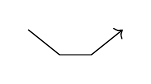
\begin{tikzpicture}[scale=0.4]
		\draw[->] (0, 0.8) -- (1, 0) -- (2, 0) -- (3, 0.8);
	\end{tikzpicture}
	的合成无关 $\Hom$ 集的加法结构, 仅涉及范畴中的有限积, 有限余积及其特例零对象, 以及它们带有的典范态射.
	
	对于 (iii), 回忆到所有有限积 (或有限余积) 皆可由零对象和双积 $\oplus$ 来构造.

	若 $(F, G)$ 为伴随对, 则 $F$ 保 $\varinjlim$ 而 $G$ 保 $\varprojlim$, 见 \cite[定理 2.8.12]{Li1}; 另一方面, 等价保所有极限. 因此 (iv) 和 (v) 都是 (ii) 的特例.
\end{proof}

事实上, 命题 \ref{prop:additive-cat-addition} 对加法的描述表明加性范畴 $\mathcal{C}$ 的``加性''乃是范畴 $\mathcal{C}$ 的一种性质, 而非额外的结构.

\begin{definition}
	\index{he@核 (kernel)} \index[sym1]{kerf@$\Ker(f)$}
	\index{yuhe@余核 (cokernel)}\index[sym1]{cokerf@$\Coker(f)$}
	设 $\mathcal{C}$ 为具有零对象的 $\cate{Ab}$-范畴, $f: X \to Y$ 为 $\mathcal{C}$ 中的态射.
	\begin{itemize}
		\item 若等化子 $\Ker(f,0)$ 存在, 则称 $\Ker(f) := \Ker(f,0)$ 连同 $\Ker(f) \hookrightarrow X$ 为 $f$ 的\emph{核}.
		\item 若余等化子 $\Coker(f,0)$ 存在, 则称 $\Coker(f) := \Coker(f,0)$ 连同 $Y \twoheadrightarrow \Coker(f)$ 为 $f$ 的\emph{余核}.
	\end{itemize}
	特别地, $\Ker(f) \to X \to Y$ 和 $X \to Y \to \Coker(f)$ 的合成按定义都是 $0$.
\end{definition}

对核以及余核, 可以有几种互补的视角.
\begin{itemize}
	\item 先考虑 $\Ker(f)$. 对任意态射 $g: T \to X$, 既然 $T \xrightarrow{g} X \xrightarrow{0} Y$ 的合成必为 $0$, 于是 $\Ker(f) = \Ker(f,0)$ 作为等化子的泛性质可表述为交换图表:
	\[\begin{tikzcd}
		& T \arrow[dashrightarrow, ld, "{\exists! g'}"'] \arrow[d, "g"] \arrow[rd, "0"] & \\
		\Ker(f) \arrow[r] & X \arrow[r, "f"'] & Y .
	\end{tikzcd}\]
	\item 考虑 $\Coker(f)$. 对任意态射 $h: Y \to T$, 既然 $X \xrightarrow{0} Y \xrightarrow{h} T$ 的合成必为 $0$. 于是 $\Coker(f) = \Coker(f, 0)$ 作为余等化子的泛性质可表述为交换图表:
	\[\begin{tikzcd}
		X \arrow[r, "f"] \arrow[rd, "0"'] & Y \arrow[r] \arrow[d, "h"] & \Coker(f) \arrow[dashrightarrow, ld, "{\exists! h'}"] . \\
		& T &
	\end{tikzcd}\]
	\item 以上两者显然相互对偶: $\Coker(f) = \Ker(f^{\opp})$, $\Ker(f) = \Coker(f^{\opp})$.
\end{itemize}

由于通过零对象分解的态射正是 $0$, 泛性质也有基于拉回和推出图表的刻画, 请读者疾速验证:
\begin{equation}\label{eqn:Ker-Coker-triangles}
	\begin{tikzcd}
		\Ker(f) \arrow[phantom, r, "\simeq" description] & X \dtimes{Y} 0 \arrow[r] \arrow[d] \arrow[phantom, rd, "\Box" description] & X \arrow[d, "f"] \\
		& 0 \arrow[r] & Y
	\end{tikzcd} \qquad \begin{tikzcd}
		X \arrow[r, "f"] \arrow[d] & Y \arrow[d] & \\
		0 \arrow[r] & Y \dsqcup{X} 0 \arrow[phantom, lu, "\boxplus" description] & \Coker(f) \arrow[phantom, l, "\simeq" description] .
\end{tikzcd}\end{equation}

\begin{remark}\label{rem:equalizer-Ker}
	一般的等化子 $\Ker(f,g)$ 可以化约到上述的核: 考虑态射
	\[\begin{tikzcd}
	T \arrow[r, "h"] & X \arrow[r, yshift=0.2em, "f"] \arrow[r, yshift=-0.2em, "g"'] & Y
	\end{tikzcd}, \]
	条件 $fh = gh$ 等价于 $(f-g)h = 0$, 由此立得 $\Ker(f,g) = \Ker(f-g, 0) =: \Ker(f-g)$. 对偶地, $\Coker(f,g) = \Coker(f-g,0) =: \Coker(f-g)$.
\end{remark}

今后主要考虑 $\mathcal{C}$ 为加性范畴的情形.

\begin{proposition}\label{prop:Ker-Coker-composite}
	对于加性范畴 $\mathcal{C}$ 中的态射 $X \xrightarrow{f} Y \xrightarrow{g} Z$, 存在交换图表
	\[\begin{tikzcd}[row sep=small, column sep=small]
		\Ker(gf) \arrow[rr, "\sim"] \arrow[hookrightarrow, rd] & & X \dtimes{Y} \Ker(g) \arrow[hookrightarrow, ld] \\
		& X &
	\end{tikzcd} \quad \begin{tikzcd}[row sep=small, column sep=small]
		Z \dsqcup{Y} \Coker(f) \arrow[rr, "\sim"] & & \Coker(gf) \\
		& Z \arrow[twoheadrightarrow, lu] \arrow[twoheadrightarrow, ru] &
	\end{tikzcd}\]
	其中 $X \dtimes{Y} \Ker(g) \to X$ (或 $Z \to Z \dsqcup{Y} \Coker(f)$) 是纤维积 (或余积) 自带的典范态射, 前提是所论的 $\Ker$, $\Coker$ 和极限皆存在.
\end{proposition}
\begin{proof}
	基于 \eqref{eqn:Ker-Coker-triangles}, 分段作纤维积得典范同构 $\Ker(gf) \simeq X \dtimes{Z} 0 \simeq X \dtimes{Y} (Y \dtimes{Z} 0) \simeq X \dtimes{Y} \Ker(g)$. 对偶性给出 $\Coker(gf)$ 的情形.
\end{proof}

等化子及余等化子的函子性诱导核及余核的函子性, 以交换图表刻画为
\begin{equation}\label{eqn:Ker-Coker-functoriality}\begin{tikzcd}
		\Ker(f) \arrow[r] \arrow[dashrightarrow, d, "\exists!"'] & X \arrow[d, "a"'] \arrow[r, "f"] & Y \arrow[d, "b"] \\
		\Ker(g) \arrow[r] & X' \arrow[r, "g"'] & Y'
	\end{tikzcd} \qquad \begin{tikzcd}
		X \arrow[d, "a"'] \arrow[r, "f"] & Y \arrow[d, "b"] \arrow[r] & \Coker(f) \arrow[dashrightarrow, d, "\exists!"'] \\
		X' \arrow[r, "g"'] & Y' \arrow[r] & \Coker(g) .
\end{tikzcd}\end{equation}

以下结果说明拉回 (或推出) 保核 (或余核).
\begin{proposition}\label{prop:pull-back-ker}
	若加性范畴 $\mathcal{C}$ 中的图表
	\[\begin{tikzcd}
		X \arrow[r, "f"] \arrow[d, "a"'] & Y \arrow[d, "b"] \\
		X' \arrow[r, "g"'] & Y'
	\end{tikzcd}\]
	是拉回 (或推出) 图表, 则 \eqref{eqn:Ker-Coker-functoriality} 的态射 $\Ker(f) \to \Ker(g)$ (或 $\Coker(f) \to \Coker(g)$) 为同构, 前提是所论的 $\Ker$ 和 $\Coker$ 存在.
\end{proposition}
\begin{proof}
	对偶性将论证归结为拉回的情形. 对任意对象 $T$, 由泛性质可以验证
	\begin{align*}
		\Hom(T, \Ker(f)) & \simeq \Ker\left[ \Hom(T, X) \to \Hom(T, Y) \right] \\
		& \simeq \Ker\left[ \Hom(T, Y) \dtimes{\Hom(T, Y')} \Hom(T, X') \to \Hom(T, Y) \right] \\
		& = \Ker\left[ \Hom(T, X') \to \Hom(T, Y') \right] \simeq \Hom(T, \Ker(g)),
	\end{align*}
	其中每个箭头都是典范的. 米田引理遂蕴涵 $\Ker(f) \rightiso \Ker(g)$; 详见定理 \ref{prop:Yoneda} 的回顾.
\end{proof}

\begin{lemma}\label{prop:mono-epi-ker-coker}
	设 $\mathcal{C}$ 为加性范畴, $f: X \to Y$ 为 $\mathcal{C}$ 中的态射, 则:
	\begin{enumerate}[(i)]
		\item $f$ 是单态射 (或满态射) 当且仅当 $\Ker(f) = 0$ (或 $\Coker(f) = 0$);
		\item $f$ 是零态射等价于 $\Ker(f) \rightiso X$, 也等价于 $Y \rightiso \Coker(f)$;
		\item 给定 $k: Y \to Z$ (或 $k': W \to X$), 存在唯一的交换图表如下:
		\[\begin{tikzcd}[row sep=small, column sep=small]
		\Ker(kf) \arrow[rd] & & \Ker(f) \arrow[ld] \arrow[hookrightarrow, ll, "\exists !"'] \\
		& X &
		\end{tikzcd} \quad \text{或} \quad
		\begin{tikzcd}[row sep=small, column sep=small]
		\Coker(fk') \arrow[twoheadrightarrow, rr, "\exists !"] & & \Coker(f) \\
		& Y \arrow[lu] \arrow[ru] &
		\end{tikzcd}\]
		前提是所论的核 (或余核) 存在. 若 $k$ 单 (或 $k'$ 满), 则 $\Ker(f) \rightiso \Ker(kf)$ (或 $\Coker(fk') \rightiso \Coker(f)$).
	\end{enumerate}
\end{lemma}
\begin{proof}
	先考虑 (i). 基于对偶性, 仅需处理单态射情形. 按定义, $f$ 为单态射等价于对任一对态射 $g_1, g_2: T \to X$ 都有 $f(g_1 - g_2) = 0 \iff g_1 - g_2 = 0$. 这相当于说对任意 $g: T \to X$, 下式成立: $f g = 0$ 当且仅当 $g$ 分解为 $T \to 0 \to X$. 这无非是说零对象符合 $\Ker(f)$ 的泛性质.
	
	同理, 对 (ii) 证 $f = 0 \iff \Ker(f) \rightiso X$ 即可. 然而 $\Ker(f) = \Ker(f, 0)$, 所求的等价容易归结为等化子的定义.
	
	至于 (iii), 同样仅考虑 $\Ker$ 的情形,
	\[\begin{tikzcd}[column sep=small]
		\left\{ g \in \Hom(T, X): fg=0 \right\} \arrow[phantom, r, "\subset" description] & \left\{ g \in \Hom(T, X): kfg=0 \right\} \\
		\Hom(T, \Ker(f)) \arrow[u, "1:1"] & \Hom(T, \Ker(kf)) \arrow[u, "1:1"']
	\end{tikzcd}\]
	当 $k$ 单时第一行取等号. 应用米田引理以完成证明.
\end{proof}

在加性范畴中, 定义 \ref{def:Im-Coim} 介绍的像和余像有简单的描述.

\begin{proposition}\label{prop:Im-Coim-additive}
	\index{xiang}\index{yuxiang}\index[sym1]{imf} \index[sym1]{coimf}
	设 $f: X \to Y$ 为加性范畴 $\mathcal{C}$ 中的态射, 则有典范同构
	\begin{align*}
		\Image(f) & \simeq \Ker\left[ Y \to \Coker(f) \right] \hookrightarrow Y, \\
		\Coim(f) & \simeq \Coker\left[ \Ker(f) \to X \right] \twoheadleftarrow X ;
	\end{align*}
	前提是所论的核, 余核皆存在.
\end{proposition}
\begin{proof}
	基于对偶性, 以下仅考虑 $\Image(f)$. 考虑典范态射 $i_1, i_2: Y \to Y \dsqcup{X} Y$. 应用米田引理, 问题化为对所有 $T \in \Obj(\mathcal{C})$ 验证
	\begin{multline*}
		\Hom\left( T, \Image(f) \right) = \left\{ h: T \to Y \;\middle|\; i_1 h = i_2 h \right\} \\
		= \left\{ \begin{array}{r|l}
			h: T \to Y & \forall S \in \Obj(\mathcal{C}),\; \forall s_1, s_2: Y \to S, \\
			& s_1 f = s_2 f \implies s_1 h = s_2 h
		\end{array}\right\} \\
		\xlongequal{s := s_1 - s_2} \left\{ \begin{array}{r|l}
			h: T \to Y & \forall S \in \Obj(\mathcal{C}),\; \forall s: Y \to S, \\
			& s f = 0 \implies sh = 0
		\end{array}\right\} \\
		= \left\{ \begin{array}{r|l}
			h: T \to Y & T \xrightarrow{h} Y \twoheadrightarrow \Coker(f) \\
			& \text{合成为}\; 0
		\end{array}\right\}
		\leftiso \Hom\left( T, \Ker\left[ Y \to \Coker(f) \right] \right).
	\end{multline*}
	以上第一个等式缘于 $\Image(f) := \Ker(i_1, i_2)$. 对于第二个等式, 先将 $h$ 的条件改写为对所有 $s': Y \dsqcup{X} Y \to S$ 皆有 $s' i_1 h = s' i_2 h$, 再用纤维余积的泛性质
	\begin{align*}
		\Hom\left( Y \dsqcup{X} Y, S \right) & \xrightarrow{1:1} \Hom(Y,S) \dtimes{\Hom(X,S)} \Hom(Y,S) \\
		s' & \longmapsto \left( s' i_1, s' i_2 \right) =: (s_1, s_2).
	\end{align*}
	第四个等式是按余核泛性质化简到 $S = \Coker(f)$ 的产物.
\end{proof}

最简单的例子是当 $f$ 为零态射时, 引理 \ref{prop:mono-epi-ker-coker} (ii) 蕴涵 $\Image(f) = 0 = \Coim(f)$.

\begin{example}\label{eg:strict-morphism}
	承接例 \ref{eg:additive-category} 的讨论. 考虑范畴 $R\dcate{Mod}$. 模同态 $f: A \to B$ 总有核以及余核, 按经典方式取为 $\Ker(f) = f^{-1}(0)$ 以及 $\Coker(f) = B/\{f(a) : a \in A\}$. 据定义立见 $\Image(f)$ 是 $f$ 在集合论意义下的像, $\Coim(f) = A/\Ker(f)$, 而 \eqref{eqn:strict-morphism} 中的典范态射 $\Coim(f) \to \Image(f)$ 无非是模论里的典范同构 $A/\Ker(f) \rightiso \Image(f)$. 因此 $R\dcate{Mod}$ 中所有态射皆严格.
	
	接着考虑例 \ref{eg:additive-category} 的加性范畴 $\cate{Ban}_{\CC}$. 连续线性映射 $f: X \to Y$ 的核是寻常的 $\Ker(f) = f^{-1}(0)$, 仍是 Banach 空间; 另一方面, $\Coker(f) = Y/\overline{\left\{ f(x): x \in X \right\}}$ 带有商范数. 对之 \eqref{eqn:strict-morphism} 的态射化为
	\[\begin{tikzcd}[row sep=small, column sep=small]
	\Coim(f) \arrow[equal, r] & X/f^{-1}(0) \arrow[r] & \overline{\left\{ f(x): x \in X \right\}} \arrow[equal, r] & \Image(f) \\
	& x + f^{-1}(0) \arrow[mapsto, r] \arrow[phantom, u, "\in" description, sloped] & f(x) \arrow[phantom, u, "\in" description, sloped] &
	\end{tikzcd}\]
	右边带诱导自 $Y$ 的拓扑, 左边则带 $X$ 的商拓扑. 设 $f: X \to Y$ 为 Banach 空间之间的连续线性单射, $f$ 像稠密而非满, 此时 $\Coim(f) = X \to Y = \Image(f)$ 非同构, 因而 $\cate{Ban}_{\CC}$ 中存在非严格的态射.
\end{example}

\section{推广: 交换环上的线性范畴}\label{sec:linear-cat}
加性范畴的 $\Hom$ 集具有加法群的结构, 而在许多情景中, $\Hom$ 集还进一步带有来自某个交换环 $\Bbbk$ 的纯量乘法. 例如在 $\Bbbk\dcate{Mod}$ 中, 每个 $\Hom$ 集自然地都是 $\Bbbk$-模, 而态射的合成是 $\Bbbk$-双线性的.

\begin{definition}\label{def:cat-k-linear}
	\index{fanchou!$\Bbbk\dcate{Mod}$-}
	\index{hanzi!$\Bbbk$-线性 ($\Bbbk$-linear)}
	设 $\Bbbk$ 为交换环. 若范畴 $\mathcal{A}$ 中的 $\Hom$ 集都带有 $\Bbbk$-模结构, 使得态射合成 $\Hom(Y, Z) \times \Hom(X, Y) \to \Hom(X, Z)$ 对所有对象 $X, Y, Z$ 都是 $\Bbbk$-双线性映射, 或者换言之有交换图表
	\[\begin{tikzcd}
		\Hom(Y, Z) \times \Hom(X, Y) \arrow[d] \arrow[r, "\text{合成}"] & \Hom(X, Z) \\
		\Hom(Y, Z) \dotimes{\Bbbk} \Hom(X, Y) \arrow[ru, bend right, start anchor=east, "{\exists! \; \text{$\Bbbk$-模同态}}"']
	\end{tikzcd}  \]
	则称 $\mathcal{A}$ 同这些资料成为 $\Bbbk\dcate{Mod}$-范畴.

	设 $F: \mathcal{A} \to \mathcal{A}'$ 为 $\Bbbk\dcate{Mod}$-范畴之间的函子, 若 $\Hom(X, Y) \to \Hom(FX, FY)$ 对所有 $X, Y \in \Obj(\mathcal{A})$ 都是 $\Bbbk$-模同态, 则称 $F$ 是 $\Bbbk$-线性函子.
\end{definition}

注意到 $\Bbbk\dcate{Mod}$ 对张量积 $\otimes := \dotimes{\Bbbk}$ 成为幺半范畴, 因此 $\Bbbk\dcate{Mod}$-范畴这一称呼和 \cite[\S 3.4]{Li1} 中关于充实范畴的术语一致. 先前介绍的 $\cate{Ab}$-范畴即 $\Z\dcate{Mod}$-范畴; 相反地, 忘却 $\Bbbk\dcate{Mod}$-范畴上的纯量乘法, 就得到 $\cate{Ab}$-范畴.

\begin{example}
	仅有一个对象的 $\Bbbk\dcate{Mod}$-范畴无非是 $\Bbbk$-代数, 对应由 $\mathcal{A} \mapsto \End_{\mathcal{A}}(\star)$ 给出, 此处 $\Obj(\mathcal{A}) = \{\star\}$.
\end{example}

命题 \ref{prop:automatic-Ab-morphism} 的论证原封不动地照搬, 给出以下结果.

\begin{proposition}\label{prop:automatic-k-morphism}
	设 $\mathcal{A}$ 和 $\mathcal{A}'$ 是 $\Bbbk\dcate{Mod}$-范畴.
	\begin{enumerate}
		\item 给定一对伴随函子
		$\begin{tikzcd}
			F: \mathcal{A} \arrow[shift left, r] & \mathcal{A}' \arrow[shift left, l] : G
		\end{tikzcd}$,
		其中 $F$, $G$ 皆是 $\Bbbk$-线性的, 则伴随同构 $\Hom_{\mathcal{A}'}(F(\cdot), \cdot) \rightiso \Hom_{\mathcal{A}}(\cdot, G(\cdot))$ 是 $\Bbbk$-线性的.
		\item 对于任意 $\alpha: I \to \mathcal{A}$, 双射
		\[ \Hom_{\mathcal{A}}\left( \varinjlim \alpha, T \right) \simeq \varprojlim_{i \in \Obj(I)} \Hom_{\mathcal{A}}(\alpha(i), T), \quad T \in \Obj(\mathcal{A}) \]
		是 $\Bbbk$-线性的, 前提是极限存在. 对 $\varprojlim$ 亦同.
	\end{enumerate}
\end{proposition}

如无另外申明, 今后 $\Bbbk\dcate{Mod}$-范畴之间的函子和等价都默认为 $\Bbbk$-线性的.

\begin{definition}\label{def:k-linear-cat}
	\index{fanchou!$\Bbbk$-线性 ($\Bbbk$-linear)}
	若给定的加性范畴 $\mathcal{A}$ 带有 $\Bbbk$-线性结构, 与原有的 $\cate{Ab}$-结构相容, 则称此资料为 $\Bbbk$-线性范畴.
\end{definition}

这相当于在 \S\ref{sec:Ker-Coker} 的讨论中以 $\Bbbk\dcate{Mod}$-范畴替代 $\cate{Ab}$-范畴. 本章关于加性范畴的结果多数能扩及 $\Bbbk$-线性的情形, 论证并无二致. 唯一的例外关乎推论 \ref{prop:automatic-additivity}: 在加性范畴中, $\Hom$ 集的加法能由范畴本身的性质来刻画, 但论及 $\Bbbk$-纯量乘法则不然; 相应地, $\Bbbk$-线性范畴之间的函子 (乃至于等价) 没有自动成为 $\Bbbk$-线性的理由.

以下搜集关于 $\Bbbk$-线性的几则结果. 回顾任意范畴 $\mathcal{A}$ 的\emph{中心}
\index{zhongxin@中心 (center)} \index[sym1]{ZA@$Z(\mathcal{A})$}
$Z(\mathcal{A}) := \End(\identity_{\mathcal{A}})$, 其元素是恒等函子 $\identity_{\mathcal{A}}$ 到自身的态射, 写作 $(a_X)_{X \in \Obj(\mathcal{A})}$, 其中 $a_X \in \End_{\mathcal{A}}(X)$. 中心对态射合成构成交换幺半群; 见 \cite[定义 2.3.8, 命题 2.3.9]{Li1}. 若 $\mathcal{A}$ 是 $\cate{Ab}$-范畴, 则 $Z(\mathcal{A})$ 相对于合成与加法 $(a_X)_X + (b_X)_X := (a_X + b_X)_X$ 成为交换环.

\begin{proposition}\label{prop:k-linear-center}
	设 $\mathcal{A}$ 为 $\cate{Ab}$-范畴, 则有双射
	\[ \left\{ \text{$\mathcal{A}$ 上的 $\Bbbk\dcate{Mod}$-范畴结构} \right\} \stackrel{1:1}{\longleftrightarrow} \Hom_{\text{环}}(\Bbbk, Z(\mathcal{A})). \]
	映法如下. 若指定了 $\mathcal{A}$ 上的 $\Bbbk\dcate{Mod}$-范畴结构, 对每个 $a \in \Bbbk$ 和 $X \in \Obj(\mathcal{A})$, 定义 $a_X := a \cdot \identity_X \in \End_{\mathcal{A}}(X)$, 则 $a \mapsto (a_X)_{X \in \Obj(\mathcal{A})} \in Z(\mathcal{A})$ 是环同态. 反之, 给定属于右式的环同态 $a \mapsto (a_X)_{X \in \Obj(\mathcal{A})}$, 以 $a \cdot f := f \circ a_X = a_Y \circ f$ 定义 $\mathcal{A}$ 上的 $\Bbbk\dcate{Mod}$-范畴结构, 其中 $f \in \Hom(X, Y)$.
\end{proposition}
\begin{proof}
	刻画 $(a_X)_{X \in \Obj(\mathcal{A})} \in Z(\mathcal{A})$ 的条件正是 $f \circ a_X = a_Y \circ f$, 其中 $f \in \Hom(X, Y)$ 任取. 若 $\mathcal{A}$ 带有 $\Bbbk\dcate{Mod}$-范畴结构, 命 $a_X := a \cdot \identity_X$, 则双线性蕴涵 $f \circ a_X = f \circ (a \cdot \identity_X) = (a f) \circ \identity_X = (a \cdot \identity_Y) \circ f = a_Y \circ f$, 故 $(a_X)_{X \in \Obj(\mathcal{A})} \in Z(\mathcal{A})$. 其余验证是平凡的.
\end{proof}

作为推论, $\cate{Ab}$-范畴 $\mathcal{A}$ 自然地成为 $Z(\mathcal{A})\dcate{Mod}$-范畴.

\section{由函子观极限}\label{sec:limit-functor}
函子 $F: \mathcal{C} \to \mathcal{D}$ 和极限间的种种关系大致可以分成两个方向. 以 $\varinjlim$ 为例, 给定函子 $\alpha: I \to \mathcal{C}$, 试问:
\begin{itemize}
	\item 设 $\varinjlim \alpha$ 存在, 其像 $F\left(\varinjlim \alpha\right)$ 是否给出 $\varinjlim (F\alpha)$?
	\item 设 $\varinjlim F\alpha$ 存在, 它能否``提升''到 $\mathcal{C}$ 上? 此提升在何种意义下唯一?
\end{itemize}

此处主要讨论 $\varinjlim$ 的情形; 这些结果对于 $\varprojlim$ 当然也有对应的版本; 鉴于对偶性, 细节不必重复.

我们以锥和范畴 $(\alpha/\Delta)$ 的语言来梳理 $\varinjlim$.

\begin{convention}\label{con:limit-cone}
	相对于给定的函子 $\alpha: I \to \mathcal{C}$, 称 $\mathcal{C}$ 中满足下述条件的资料 $(L, (f_i)_{i \in \Obj(I)})$ 为以 $\alpha$ 为底, 以 $L$ 为顶点的\emph{锥}:
	\begin{compactitem}
		\item $L$ 是 $\mathcal{C}$ 的对象,
		\item 每个 $f_i : \alpha(i) \to L$ 都是 $\mathcal{C}$ 的态射, 具备相容性条件 $f_j \circ \alpha(i \to j) = f_i$, 其中 $[i \to j]$ 取遍 $\mathrm{Mor}(I)$.
	\end{compactitem}
\end{convention}

按 \cite[\S 2.7]{Li1} 的语言, 这些锥构成范畴\footnote{此处 $\Delta$ 的严格含义是对角函子 $\mathcal{C} \to \mathcal{C}^I$, 见例 \ref{eg:comma-vs-cone}, 按拼音命名. 但也无妨按照象形原则将 $\Delta$ 想成``锥'', 见图 \eqref{eqn:injlim-diagram}.} $(\alpha / \Delta)$; 具体地说, 当底 $\alpha$ 固定, 从锥 $(L, (f_i)_i)$ 到锥 $(M, (g_i)_i)$ 的态射是交换图表
\begin{equation}\label{eqn:injlim-diagram}\begin{tikzcd}
	& L \arrow[d] & \\
	\alpha(i) \arrow[bend right, rr, "\alpha(i \to j)"'] \arrow[r, "g_i"] \arrow[ru, "f_i"] & M & \alpha(j) \arrow[l, "{g_j}"'] \arrow[lu, "f_j"']
\end{tikzcd}\end{equation}
其中 $i \to j$ 取遍 $\Mor(I)$, 态射合成按明显的方式操作. 按定义, $\varinjlim \alpha$ 连同其自带的典范态射族 $\iota_i: \alpha(i) \to \varinjlim \alpha$ 是 $(\alpha / \Delta)$ 的始对象.
\index{jixian}\index[sym1]{lim}

函子 $F$ 按自明的方式诱导函子 $(\alpha/\Delta) \to (F\alpha / \Delta)$, 映锥 $(L, (f_i)_i)$ 为 $(FL, (Ff_i)_i)$. 设 $\varinjlim \alpha$ 存在, 倘若 $\varinjlim F\alpha$ 也存在, 则在 $(F\alpha / \Delta)$ 中存在唯一态射
\[ \varinjlim F\alpha \to F(\varinjlim \alpha), \]
它是同构当且仅当 $\left( F(\varinjlim \alpha), (F\iota_i)_i \right)$ 给出 $\varinjlim F\alpha$.

倒转箭头, $\varprojlim \alpha$ 可刻画为 $(\Delta/\alpha)$ 的终对象. 在所论 $\varprojlim$ 存在的前提下, 在 $(\Delta/F\alpha)$ 中存在唯一态射
\[ F\varprojlim \alpha \to \varprojlim F\alpha. \]

\begin{definition}\label{def:create-limit}
	\index{jixian!保, 返, 生 (preserve, reflect, create)}
	给定 $F: \mathcal{C} \to \mathcal{D}$ 和函子 $\alpha: I \to \mathcal{C}$, 考虑锥范畴之间的函子 $(\alpha/\Delta) \to (F\alpha/\Delta)$.
	\begin{itemize}
		\item 称 $F$ \emph{保}此 $\varinjlim$, 如果 $(\alpha/\Delta) \to (F\alpha/\Delta)$ 映始对象 (假如存在) 为始对象.
		\item 称 $F$ \emph{返}此 $\varinjlim$, 如果仅 $(\alpha/\Delta)$ 的始对象 (假如存在) 方能被映为 $(F\alpha/\Delta)$ 的始对象.
		\item 称 $F$ \emph{生}此 $\varinjlim$, 如果
		\begin{compactitem}
			\item $\varinjlim F\alpha \;\text{存在} \implies \varinjlim \alpha \;\text{存在}$;
			\item $F$ 保此 $\varinjlim$, 返此 $\varinjlim$.
		\end{compactitem}
	\end{itemize}
	对于 $\varprojlim$ 同样有相应的概念, 以 $\mathcal{C}^{\opp}$ 和 $\mathcal{D}^{\opp}$ 代 $\mathcal{C}$ 和 $\mathcal{D}$ 即可相互过渡.
\end{definition}

注意: 这些概念系于所论的 $\alpha$, 比如 $F$ 完全有可能保有限的 $\varinjlim$ 而不保一般的 $\varinjlim$.

给定 $\alpha$, 函子生 $\varinjlim$ (或 $\varprojlim$) 相当于说 $\mathcal{D}$ 中定义此极限的锥可以唯一地提升到 $\mathcal{C}$, 并且使后者给出 $\mathcal{C}$ 中相应的极限; 唯一性来自定义中关于返 $\varinjlim$ (或 $\varprojlim$) 的条件. 这一观点将在稍后的例 \ref{eg:Grp-Set-create} 和命题 \ref{prop:forget-create} 中清楚呈现. 

\begin{proposition}\label{prop:ff-reflect}
	全忠实函子返一切 $\varinjlim$ 和 $\varprojlim$.
\end{proposition}
\begin{proof}
	以 $\varinjlim$ 为例. 设 $F$ 全忠实, 则 $(\alpha/\Delta)$ 的始对象的泛性质可在取 $F$ 后在 $(F\alpha/\Delta)$ 中验证.
\end{proof}

顺势引入一个方便的概念.
\begin{definition}\label{def:conservative}
	\index{hanzi!保守 (conservative)}
	满足以下条件的函子 $F$ 称为\emph{保守}的: 态射 $f \in \Mor(\mathcal{C})$ 为同构当且仅当 $Ff \in \Mor(\mathcal{D})$ 为同构. 
\end{definition}

\begin{remark}\label{rem:conservative-reflect}
	若 $F$ 是保守函子, 则只要 $\varinjlim \alpha$ 存在, 而且 $F$ 保此 $\varinjlim$, 则 $F$ 也必然返此 $\varinjlim$. 缘由如下: 设 $L \in \Obj((\alpha/\Delta))$ 被映为 $(F\alpha/\Delta)$ 的始对象; 考虑 $(\alpha/\Delta)$ 中的唯一态射 $\varinjlim \alpha \to L$, 由于 $F$ 保此 $\varinjlim$, 它在 $F$ 之下的像必为同构, 从而保守条件确保 $\varinjlim \alpha \to L$ 也是同构.
	
	在此前提下, 关于 $F$ 生 $\varinjlim$ 的定义中可以去除返 $\varinjlim$ 的条件.
\end{remark}

\begin{example}\label{eg:Grp-Set-create}
	以下来验证从群范畴 $\cate{Grp}$ 到集合范畴 $\cate{Set}$ 的忘却函子 $U$ 生所有小 $\varprojlim$.
	
	这是 $\varprojlim$ 在 $\cate{Grp}$ 和 $\cate{Set}$ 中的具体构造的推论, 见 \cite[例 2.7.5 和 2.8.7]{Li1}. 详言之, 取小范畴 $I$ 和函子 $\beta: I^{\opp} \to \cate{Grp}$. 作为集合,
	\[ \varprojlim U\beta = \left\{\begin{array}{r|l}
		(x_i)_i \in \prod_{i \in \Obj(I)} U\beta(i) & \forall [i \to j] \in \mathrm{Mor}(I), \\
		& \beta(i \to j)(x_j) = x_i
	\end{array}\right\}, \]
	投影 $p_i: \varprojlim U\beta \to U\beta(i)$ 映 $(x_j)_j$ 为 $x_i$. 眼下的任务是:
	\begin{enumerate}
		\item 赋予 $\varprojlim U\beta$ 群结构, 使得每个 $p_i$ 都是群同态, 并说明这样的群结构唯一;
		\item 对此群连同投影同态族 $(p_i)_i$ 验证 $\varprojlim \beta$ 的泛性质. 
	\end{enumerate}

	显然 $\varprojlim U\beta$ 是直积 $\prod_i \beta(i)$ 的子群, 记为 $\varprojlim \beta \in \Obj(\cate{Grp})$, 这是使每个 $p_i$ 皆为群同态的唯一群结构. 这就完成了第一点.
	
	接着对锥 $\left( \varprojlim \beta, (p_i)_i\right)$ 验证泛性质. 考虑 $\cate{Grp}$ 中任意的锥 $(L, (q_i)_i)$, 其中 $q_i: L \to \beta(i)$. 泛性质给出唯一的映射 $\varphi: UL \to \varprojlim U\beta$ 使得 $p_i \varphi = q_i$ 恒成立. 事实上 $\varphi$ 具体写作 $y \mapsto (q_i(y))_{i \in \Obj(I)}$, 故它升级为群同态 $L \to \varinjlim \beta$. 验证完毕.
\end{example}

基于完全类似的论证, 可以说明从紧 Hausdorff 空间范畴 $\cate{CHaus}$ 到 $\cate{Set}$ 的忘却函子也生所有小 $\varprojlim$. 相关验证属于本章习题.

次一则结果涉及形如 $\mathcal{C}^J$ 的函子范畴 (可能是``大''范畴, 但无妨), 这需要两步准备.

\begin{itemize}
	\item 设 $J$ 为集合, $J$ 份 $\mathcal{C}$ 的积 $\mathcal{C}^J$ 定义为: $\Obj\left(\mathcal{C}^J\right) = \Obj(\mathcal{C})^J$, $\mathrm{Mor}\left(\mathcal{C}^J \right) = \mathrm{Mor}(\mathcal{C})^J$. 对每个 $j \in J$ 皆有自明的投影函子 $p_j: \mathcal{C}^J \to \mathcal{C}$.

	给定范畴 $I$ 和函子 $\alpha: I \to \mathcal{C}^J$, 若对对每个 $j$ 都存在 $\varinjlim (p_j \alpha)$, 则 $\varinjlim \alpha$ 也存在, 其构造方式是``逐点''或曰``逐对象''地取极限: $\varinjlim \alpha = \left( \varinjlim (p_j \alpha) \right)_{j \in J}$.

	\item 设 $J$ 为范畴, 对之可考虑函子范畴 $\mathcal{C}^J$. 对每个 $j \in \Obj(J)$ 都有求值函子 $\mathrm{ev}_j: \mathcal{C}^J \to \mathcal{C}$, 映对象 $F$ 为 $Fj$, 映态射 $\varphi = (\varphi_{j'})_{j' \in \Obj(J)}$ 为 $\varphi_j$. 稍后将考虑形如 $\alpha: I \to \mathcal{C}^J$ 的函子及其 $\varinjlim$; 注意到 $\alpha$ 可视同函子 $I \times J \to \mathcal{C}$, 取值写作 $\alpha(i, j)$.
\end{itemize}

两套符号是兼容的: 若 $J$ 是离散范畴, 视之为集合, 则 $\mathcal{C}^J$ 无非是先前讨论的积. 对于一般的 $J$, 忘却函子 $\mathcal{F}: \mathcal{C}^J \to \mathcal{C}^{\Obj(J)}$ 映对象 $F$ 为 $(Fj)_{j \in \Obj(J)}$, 映态射 $\varphi$ 为 $(\varphi_j)_{j \in \Obj(J)}$. 因此 $\mathrm{ev}_j = p_j \mathcal{F}$.

\begin{proposition}\label{prop:forget-create}
	设 $J$ 和 $\mathcal{C}$ 为范畴.
	\begin{enumerate}[(i)]
		\item 忘却函子 $\mathcal{F}: \mathcal{C}^J \to \mathcal{C}^{\Obj(J)}$ 生 $\varinjlim$ 和 $\varprojlim$.
		\item 设 $I$ 为范畴, 而且所有始自 $I$ 的函子在 $\mathcal{C}$ 中皆有 $\varinjlim$ (或 $\varprojlim$), 则所有形如 $I \to \mathcal{C}^J$ 的函子在 $\mathcal{C}^J$ 中也有 $\varinjlim$ (或 $\varprojlim$).
		\item 承上, 对每个 $j \in \Obj(J)$, 求值函子 $\mathrm{ev}_j: \mathcal{C}^J \to \mathcal{C}$ 保这些 $I$ 给出的 $\varinjlim$ (或 $\varprojlim$); 换言之, $\mathcal{C}^J$ 中的极限也是``逐点''或逐对象地定义的.
	\end{enumerate}
\end{proposition}
\begin{proof}
	考虑 $\varinjlim$ 情形即可. 对于 (i), 选定 $\alpha: I \to \mathcal{C}^J$, 假设 $\varinjlim \mathcal{F}\alpha$ 存在, 由锥
	\[ \left( (X(j))_{j \in \Obj(J)}, \; \left( \iota_i = (\iota_{i, j})_{j \in \Obj(J)} \right)_{i \in \Obj(I)} \right) \]
	给出, 其中 $\iota_{i,j}: \alpha(i, j) \to X(j)$. 我们希望将它提升为 $\mathcal{C}^J$ 中的锥, 使之给出 $\varinjlim \alpha$.
	
	首先观察对所有 $j$ 必有 $X(j) = \varinjlim \alpha(\cdot, j)$. 对于所有态射 $j \to j'$, 极限的函子性 (见 \cite[引理 2.7.4]{Li1}) 遂给出唯一的态射 $X(j \to j'): X(j) \to X(j')$ 使下图交换
	\[\begin{tikzcd}
		\alpha(i, j) \arrow[r] \arrow[d, "{\iota_{i, j}}"'] & \alpha(i, j') \arrow[d, "{\iota_{i, j'}}"] \\
		X(j) \arrow[r, "{X(j \to j')}"'] & X(j')
	\end{tikzcd} \quad i \in \Obj(I). \]
	依此升级 $j \mapsto X(j)$ 为函子 $X: J \to \mathcal{C}$, 升级 $\iota_i: \alpha(i, \cdot) \to X$ 为 $\mathcal{C}^J$ 的态射. 不难验证 $(X, (\iota_i)_i) \in \Obj(\alpha/\Delta)$, 以下验证它是始对象. 由于函子 $\mathcal{F}$ 保守, 返 $\varinjlim$ 的条件不用再验证.

	给定 $(L, (f_i)_i) \in \Obj(\alpha/\Delta)$, 由 $\varinjlim \mathcal{F}\alpha$ 的泛性质确定唯一的态射 $\varphi = (\varphi_j)_j : \mathcal{F}X \to \mathcal{F}L$, 使下图三角部分对所有 $(i, j)$ 交换:
	\[\begin{tikzcd}
		& X(j) \arrow[d, "\varphi_j"] \arrow[r, "{X(j \to j')}" inner sep=0.8em] & X(j') \arrow[d, "\varphi_{j'}"] \\
		\alpha(i, j) \arrow[ru, "{\iota_{i,j}}"] \arrow[r, "f_{i, j}"' inner sep=0.8em] & L(j) \arrow[r, "{L(j \to j')}"' inner sep=0.8em] & L(j')
	\end{tikzcd}\]
	若能说明方块对所有 $j \to j'$ 皆交换, 则 $\varphi$ 升级为 $X \to L$. 外框已知交换, 故
	\[ \varphi_{j'} X(j \to j') \iota_{i, j} = L(j \to j') f_{i, j} = L(j \to j') \varphi_j \iota_{i, j} \]
	对所有 $i$ 成立; 始自 $X(j)$ 的态射由它和所有 $\iota_{i,j}$ 的合成确定, 故方块交换.

	至于 (ii), 考虑函子 $\alpha: I \to \mathcal{C}^J$. 根据此前讨论, $\mathcal{F}\alpha: I \to \mathcal{C}^{\Obj(J)}$ 有 $\varinjlim$, 它是逐对象地定义的. 由 (i) 可在 $\mathcal{C}$ 中生出 $\varinjlim \alpha$, 而关于 $\mathrm{ev}_j$ 保这些 $\varinjlim$ 的断言 (iii) 则是构造的直接结论.
\end{proof}

\section{滤过归纳极限}\label{sec:filtered-indlim}
数学分析的一则常识是数列的极限可以由任何子数列来计算, 这点在范畴论中体现为共尾的概念. 我们先从连通性切入.

\begin{definition}\index{fanchou!连通 (connected)}
	设 $I$ 为任意范畴, 若 $\Obj(I) \neq \emptyset$, 而且对任何 $i, i' \in \Obj(I)$, 总存在 $n \geq 1$ 和态射
	\[ i = i_0 \leftarrow i_1 \to i_2 \leftarrow i_3 \to i_4 \leftarrow \cdots \to i_{2n} = i' , \]
	则称 $I$ 是连通的.
\end{definition}

介绍一则辅助概念, 后续几节将反复运用.

\begin{definition}[逗号范畴, 见 {\cite[定义 2.4.7]{Li1}}]\label{def:comma-category}
	\index{douhaofanchou@逗号范畴 (comma category)}
	\index[sym1]{iHHi@$(i/H)$, $(H/i)$}
	\index[sym1]{Pii@$\Pi_{i/}$, $\Pi_{/i}$}
	给定范畴 $I$, $J$ 和函子 $H: J \to I$. 设 $i \in \Obj(I)$.
	\begin{itemize}
		\item 按定义, 逗号范畴 $(i/H)$ (或 $(H/i)$) 的对象是资料 $(j, i \to Hj)$ (或 $(j, Hj \to i)$), 其中 $j \in \Obj(J)$ 而 $i \to Hj$ (或 $Hj \to i$) 是 $I$ 的态射; 资料之间的态射是 $J$ 中使下图交换的态射 $f: j \to j'$:
		\[\begin{tikzcd}[row sep=small, column sep=small]
			& i \arrow[ld] \arrow[rd] & \\
			Hj \arrow[rr, "{Hf}"'] & & Hj'
		\end{tikzcd} \quad \text{或} \quad \begin{tikzcd}[row sep=small, column sep=small]
			& i & \\
			Hj \arrow[ru] \arrow[rr, "{Hf}"'] & & Hj' \arrow[lu] .
		\end{tikzcd}\]
		态射合成与恒等态射的定义是自明的.
		\item 上述范畴分别带有投影函子 $\Pi_{i/}: (i/H) \to J$ 和 $\Pi_{/i}: (H/i) \to J$, 映对象 $(j, i \to Hj)$ (或 $(j, Hj \to i)$) 为 $j$, 映态射 $f$ 为 $f$.
		\item 任何 $I$ 中的态射 $i \to i'$ 皆诱导自明的函子 $(i'/H) \to (i/H)$ 和 $(H/i) \to (H/i')$, 使下图交换:
		\[\begin{tikzcd}[column sep=small, row sep=small]
			(i'/H) \arrow[rr] \arrow[rd, "{\Pi_{i'/}}"'] & & (i/H) \arrow[ld, "{\Pi_{i/}}"] \\
			& J &
		\end{tikzcd} \quad \begin{tikzcd}[column sep=small, row sep=small]
			(H/i) \arrow[rr] \arrow[rd, "{\Pi_{/i}}"'] & & (H/i') \arrow[ld, "{\Pi_{/i'}}"] . \\
			& J &
		\end{tikzcd}\]
	\end{itemize}
\end{definition}

\begin{example}\label{eg:comma-vs-cone}
	考虑函子 $\alpha: I \to \mathcal{C}$, 视同 $\mathcal{C}^I$ 的对象, 另外考虑对角函子 $\Delta: \mathcal{C} \to \mathcal{C}^I$, 映任意对象为对应的常值函子. 定义 \ref{def:comma-category} 的 $(\alpha/\Delta)$ 无非是约定 \ref{con:limit-cone} 介绍的``锥''范畴, 而函子 $\Pi_{\alpha/}$ 萃取锥的顶点.
\end{example}

\begin{definition}\label{def:cofinal} \index{gongwei@共尾 (cofinal)}
	对于函子 $H: J \to I$, 若 $(i/H)$ 对每个 $i \in \Obj(I)$ 皆连通, 则称 $H$ \emph{共尾}; 若 $H$ 是子范畴的嵌入态射, 则称子范畴 $J$ 共尾.
\end{definition}

容易验证若 $I \to J$ 和 $J \to K$ 皆共尾, 则合成函子 $I \to K$ 亦然. 请读者练习.

以下结果说明极限可以在共尾的范畴中计算. 回忆到 $H$ 诱导 $H^{\opp}: J^{\opp} \to I^{\opp}$.

\begin{proposition}\label{prop:cofinal-lim}
	若 $H: J \to I$ 共尾, 则:
	\begin{itemize}
		\item 当 $\alpha: I \to \mathcal{C}$ 给定, $\varinjlim \alpha$ 存在当且仅当 $\varinjlim \alpha H$ 存在, 此时有典范同构 $\varinjlim \alpha H \simeq \varinjlim \alpha$;
		\item 对偶地, 当 $\beta: I^{\opp} \to \mathcal{C}$ 给定, $\varprojlim \beta$ 存在当且仅当 $\varprojlim \beta H^{\opp}$ 存在, 此时有典范同构 $\varprojlim \beta H^{\opp} \simeq \varprojlim \beta$.
	\end{itemize}
\end{proposition}
\begin{proof}
	仅处理 $\varinjlim$. 依照 \S\ref{sec:limit-functor} 的语言, 证明函子 $(\alpha/\Delta) \to (\alpha H / \Delta)$ 为等价即可; 它映以 $\alpha$ 为底的锥 $(L, (f_i)_i)$ 为以 $\alpha H$ 为底的锥 $(L, (f_{Hj})_j)$.

	首先证明它本质满. 考虑 $L \in \Obj(\mathcal{C})$ 和满足相容性条件 $g_{j'} \circ \alpha H(j \to j') = g_j$ 的一族态射 $g_j: \alpha H(j) \to L$, 其中 $j \in \Obj(J)$. 对任意 $i \in \Obj(I)$, 因为 $(i/H)$ 非空故可取 $j$ 和 $i \to H(j)$. 定义 $f_i := g_j \circ [\alpha(i) \to \alpha H(j)]$. 这和 $i \to H(j)$ 的选取无关: 诚然, 若有 $(i/H)$ 中的态射
	\[\begin{tikzcd}[column sep=large]
		& i \arrow[ld] \arrow[d] \arrow[rd] & \\
		H(j) & H(j'') \arrow[l, "{H(j'' \to j)}"] \arrow[r, "{H(j'' \to j')}"'] & H(j')
	\end{tikzcd}\]
	则按构造易见
	\[ g_j \circ [\alpha(i) \to \alpha H(j)] = g_{j''} \circ [\alpha(i) \to \alpha H(j'')] = g_{j'} \circ [\alpha(i) \to \alpha H(j')]. \]
	由于 $(i/H)$ 连通, 这足以说明 $f_i$ 是良定义的. 上述讨论也蕴涵 $(f_i)_i$ 满足相容性条件, 因为对于任意 $i \to i'$ 和 $i' \to H(j')$, 总可以假设 $f_i$ 是由资料 $j := j'$ 和 $i \to i' \to H(j)$ 确定的. 综上 $(L, (f_i)_i) \in \Obj((\alpha/\Delta))$ 映至 $(L, (g_j)_j)$.
	
	接着说明它全忠实. 给定 $(\alpha/\Delta)$ 的态射 $(L, (f_i)_i) \to (L', (f'_i)_i)$ 相当于给定 $\mathcal{C}$ 的态射 $\theta: L \to L'$, 使得 $\theta f_i = f'_i$ 恒成立, 而这点只须对足够``深''的 $i$ 来验证; 对每个 $i$ 取 $j \in \Obj(J)$ 以及 $i \to H(j)$, 则条件可化约为 $\theta f_{H(j)} = f'_{H(j)}$, 亦即 $\theta$ 是 $(\alpha H / \Delta)$ 的态射.
\end{proof}

\begin{definition}
	\index{fanchou!滤过 (filtered)}
	\index{jixian!滤过 (filtered)}
	根据 \cite[定义 2.7.6]{Li1}, 具备以下条件的范畴 $I$ 称为\emph{滤过}的.
	\begin{compactitem}
		\item 对所有 $i, j \in \Obj(I)$, 存在 $k \in \Obj(I)$ 和态射 $i \rightarrow k \leftarrow j$.
		\item 对 $I$ 中任一对态射 $f, g: i \to j$, 存在态射 $k \in \Obj(I)$ 和态射 $h: j \to k$, 使得 $hf = hg$.
	\end{compactitem}

	若 $I$ 是滤过范畴, $\alpha: I \to \mathcal{C}$ 是函子, 则对应的 $\varinjlim \alpha$ 也称为滤过的.
\end{definition}

\begin{example}\label{eg:filtered-poset}
	\index{pianxuji!滤过 (filtered)}
	一类常见的滤过范畴来自滤过偏序集\footnote{在作为极限的下标来运用时, 经常可以用滤过偏序集来代替滤过范畴, 详见注记 \ref{rem:filtered-poset} 和\CHref{sec:app-Abel}习题的说明.}. 任何偏序集 $(P, \leq)$ 都给出相应的范畴 $\mathcal{P}$, 使得 $x \leq y  \iff \Hom_{\mathcal{P}}(x, y) \neq \emptyset$. 如果 $\mathcal{P}$ 是滤过范畴, 则称 $(P, \leq)$ 为\emph{滤过偏序集}. 偏序集滤过当且仅当任两个元素 $i, j$ 都有共同上界 $k$. 全序集显然滤过.
\end{example}

\begin{proposition}\label{prop:cofinal-filtered}
	设 $I$ 是滤过范畴, 则全子范畴 $J$ 共尾当且仅当对每个 $i \in \Obj(I)$ 皆存在 $j \in \Obj(J)$ 和态射 $i \to j$; 此时 $J$ 也是滤过的.
\end{proposition}
\begin{proof}
	``仅当''方向显然. 对于``当''的方向, 给定 $j \leftarrow i \to j'$, 其中 $j, j' \in \Obj(J)$, 滤过性质确保存在交换图表
	\[\begin{tikzcd}[row sep=tiny, column sep=small]
		& j \arrow[r] & k & j' \arrow[l] & \\
		j \arrow[equal, ru] & & & & j' \arrow[equal, lu] \\
		& & i \arrow[llu] \arrow[uu] \arrow[rru] & &
	\end{tikzcd}\]
	使得 $k \in \Obj(J)$. 这说明 $J$ 共尾.
	
	至于 $J$ 的滤过性质, 任取 $i, j \in \Obj(J)$, 由 $I$ 滤过可知存在 $k_0 \in \Obj(I)$ 连同态射 $i \rightarrow k_0 \leftarrow j$; 再取 $k \in \Obj(J)$ 连同态射 $k_0 \to k$, 便有 $J$ 中的态射 $i \rightarrow k_0 \leftarrow j$. 至此验证了滤过范畴的第一个条件. 同样思路可处理第二个条件.
\end{proof}

\begin{example}
	命 $\mathrm{OFin}_I := \left\{ \text{全子范畴}\; J \subset I: \Obj(J) \;\text{有限} \right\}$, 它对 $\subset$ 构成滤过偏序集: 对任意 $J, K \in \mathrm{OFin}_I$, 将对象集取并便是 $J$ 和 $K$ 的共同上界.
\end{example}

这一构造有何用处? 考虑任意函子 $\alpha: I \to \mathcal{C}$ (或 $\beta: I^{\opp} \to \mathcal{C}$), 它限制到全子范畴 $J$ 上, 给出 $\alpha|_J$ (或 $\beta|_{J^{\opp}}$). 如果 $J \subset K$, 则有自然的态射 $\varinjlim \alpha|_J \to \varinjlim \alpha|_K$ (或 $\varprojlim \beta|_{K^{\opp}} \to \varprojlim \beta|_{J^{\opp}}$), 前提是所论极限存在. 以下结果解释了从对象有限的情形``滤过地''逼近任意极限的一种方法.

\begin{proposition}\label{prop:limit-filtered-approx}
	在以上情境中, 有典范同构
	\[ \varinjlim_{\substack{J \in \mathrm{OFin}_I \\ \subset}} \varinjlim \alpha|_J \rightiso \varinjlim \alpha \]
	(或 $\varprojlim \beta \rightiso \varinjlim_{\substack{J \in \mathrm{OFin}_I \\ \subset}} \varprojlim \beta|_{J^{\opp}}$ ), 前提是左式 (或右式) 的二重极限存在.
\end{proposition}
\begin{proof}
	以 $\varinjlim$ 情形为例, 泛性质给出集合的典范双射
	\[ \Hom\left( \varinjlim_J \varinjlim \alpha|_J, S \right) \simeq \varprojlim_J \Hom\left( \varinjlim \alpha|_J, S \right) \simeq \varprojlim_J \varprojlim \Hom(\alpha|_J, S) , \]
	其中 $S \in \Obj(\mathcal{C})$ 任取, 右式是集合的二重 $\varprojlim$. 问题化为对一族集合 $(X_i)_{i \in \Obj(I)}$ 连同满足相容性的态射族 $\left( f_{i \to j}: X_j \to X_i \right)_{[i \to j] \in \Mor(I)}$ 验证双射
	\[\begin{tikzcd}[row sep=tiny]
		\displaystyle\varprojlim_{i \in \Obj(I)} X_i \arrow[r, "1:1"] & \displaystyle\varprojlim_{J \in \mathrm{OFin}_I} \displaystyle\varprojlim_{j \in \Obj(J)} X_j \\
		(x_i)_i \arrow[mapsto, r] & \left( (x_j)_{j \in \Obj(J)} \right)_{J \in \mathrm{OFin}_I} .
	\end{tikzcd}\]

	对每个 $J$, 集合的 $\varprojlim$ 其具体构造是
	\[ \varprojlim_{j \in \Obj(J)} X_j = \left\{ (x_j)_j \in \prod_{j \in J} X_j : \forall [i \to j] \in \Mor(J), \; f_{i \to j}(x_j) = x_i \right\}, \]
	双射因而是明显的: $\varprojlim_i X_i$ 的每个坐标 $x_i$ 和每个相容性条件 $f_{i \to j}(x_j) = x_i$ 都能被某个 $J \in \mathrm{OFin}_I$ 捕捉.
\end{proof}
	
回忆到范畴 $\cate{Set}$ 具有所有的小 $\varinjlim$ 和 $\varprojlim$. 滤过小 $\varinjlim$ 具有特别良好的描述.

\begin{proposition}\label{prop:filtered-union}
	设 $I$ 为滤过小范畴, $\alpha: I \to \cate{Set}$ 为函子. 在集合 $\bigsqcup_{i \in \Obj(I)} \alpha(i)$ 上定义以下二元关系: 对于 $x \in \alpha(i)$ 和 $y \in \alpha(j)$, 关系 $x \sim y$ 意谓存在 $I$ 中的态射 $i \rightarrow k \leftarrow j$, 使得 $\alpha(i \to k)(x) = \alpha(j \to k)(y)$. 那么 $\sim$ 是等价关系, 而且
	\[ \varinjlim \alpha = \left( \bigsqcup_{i \in \Obj(I)} \alpha(i) \right) \big/ \sim . \]
\end{proposition}
\begin{proof}
	见诸 \cite[定义 2.7.6]{Li1} 之下的讨论.
\end{proof}

今后将上述之 $\varinjlim \alpha$ 的元素表作 $[x_{i_0}]$, 其中 $i_0 \in \Obj(I)$ 而 $[x_{i_0}]$ 为含 $x_{i_0} \in \alpha(i_0)$ 的等价类. 另一方面, 对于一般的小范畴 $J$ 和函子 $\beta: J^{\opp} \to \cate{Set}$, 我们将 $\varprojlim \beta$ 的元素表作 $(y_j)_{j \in \Obj(J)}$ 之形, 其中 $y_j \in \beta(j)$ 满足相容性条件 $\beta(j' \to j)(y_j) = y_{j'}$.

接着考虑形如 $\alpha: I \times J^{\opp} \to \cate{Set}$ 的函子, 其中 $I, J$ 是小范畴; 对变元 $I$ 和 $J$ 可以分别取 $\varinjlim$ 和 $\varprojlim$. 对于任意 $(i_0, j_0) \in \Obj(I \times J)$, 自然映射的合成
\[ \varprojlim_j \alpha(i_0, j) \to \alpha(i_0, j_0) \to \varinjlim_i \alpha(i, j_0); \]
对 $i_0$, $j_0$ 皆有函子性. 变动 $j_0$ 给出典范映射 $\varprojlim_j \alpha(i_0, j) \to \varprojlim_j \varinjlim_i \alpha(i, j)$, 继而变动 $i_0$ 以得到典范映射
\begin{equation}\label{eqn:filtered-finite-exchange}
	e: \varinjlim_i \varprojlim_j \alpha(i, j) \to \varprojlim_j \varinjlim_i \alpha(i, j).
\end{equation}
如采取代表元的记法, 则 $e$ 映 $\left[ (x_{i_0, j})_j \right]$ 为 $\left( [ x_{i_0, j}] \right)_j$.

若 $\Mor(J)$ 是有限集, 则称范畴 $J$ 是有限的; 这相当于要求对象集和任两个对象之间的态射集皆有限. 次一结果将用于 \S\ref{sec:cat-localization}.

\begin{proposition}\label{prop:filtered-finite-exchange}
	设 $I$ 为滤过小范畴, $J$ 为有限范畴, $\alpha: I \times J^{\opp} \to \cate{Set}$ 为函子. 此时 \eqref{eqn:filtered-finite-exchange} 的映射 $e$ 是双射.
\end{proposition}
\begin{proof}
	首先说明 $e$ 满. 给定 $(b_j)_{j \in \Obj(J)} \in \varprojlim_j \varinjlim_i \alpha(i, j)$, 将每个 $b_j$ 表为 $[x_{i_j, j}]$. 由于 $I$ 滤过而 $J$ 有限, 能取 $i_j$ 为常值 $i \in \Obj(I)$. 对 $J$ 中的每个态射 $j \to j'$, 我们有
	\[ \left[ \alpha(i, j \to j') (x_{i, j'}) \right] = \left[ x_{i, j} \right]. \]
	再次应用 $I$ 滤过和 $J$ 有限的性质, 可以取足够``深''的 $i \to i_1$ 并以 $i_1$ 代 $i$, 以确保 $\alpha(i, j \to j') (x_{i, j'}) = x_{i, j}$ 对所有 $[j \to j'] \in \Mor(J)$ 成立. 故 $e\left( [(x_{i, j})_j] \right) = (b_j)_j$.
	
	其次说明 $e$ 单. 设 $e(x) = e(y)$. 因为 $I$ 滤过, 可取 $i \in \Obj(I)$ 使得 $x$ 有代表元 $(x_{i, j})_j$ 而 $y$ 有代表元 $(y_{i, j})_j$, 故对所有 $j \in \Obj(J)$ 皆有 $[x_{i, j}] = [y_{i, j}]$. 因为 $I$ 滤过而 $J$ 有限, 按先前方法调整 $i$ 可确保 $x_{i, j} = y_{i, j}$ 对所有 $j$ 皆成立, 故 $x = y$.
\end{proof}


\section{Kan 延拓}\label{sec:Kan-extension}
本节从函子的延拓问题出发. 考虑范畴 $\mathcal{C}$, $\mathcal{D}$, $\mathcal{E}$ 和函子 $K$, $F$ 如下图:
\[\begin{tikzcd}
	\mathcal{C} \arrow[d, "K"'] \arrow[rd, bend left, "F"] & \\
	\mathcal{D} \arrow[dashed, r, "{\exists ? \; L}"'] & \mathcal{E}
\end{tikzcd}\]
按照范畴论的基本精神, 我们希望找到虚线所示的函子 $L$ 连同同构 $F \simeq LK$. 此问题一般无解; 例如可能存在 $f \in \Mor(\mathcal{C})$ 使得 $Kf$ 为同构, 而 $Ff$ 非同构. 退而求其次, 我们至少可以问: 是否存在一个最佳逼近? 答案由泛性质刻画, 分为左右两种版本.

\begin{definition}[D.\ Kan]\label{def:Kan-extension}
	\index{Kanyantuo@Kan 延拓 (Kan extension)}
	\index[sym1]{LanKF@$\Lan_K F$}
	\index[sym1]{RanKF@$\Ran_K F$}
	考虑范畴 $\mathcal{C}$, $\mathcal{D}$, $\mathcal{E}$, 函子 $K: \mathcal{C} \to \mathcal{D}$ 和 $F: \mathcal{C} \to \mathcal{E}$.
	\begin{itemize}
		\item 函子 $F$ 沿 $K$ 的\emph{左 Kan 延拓}意谓如下资料 $(\Lan_K F, \eta)$, 其中
		\begin{compactitem}
			\item $\Lan_K F: \mathcal{D} \to \mathcal{E}$ 是函子,
			\item $\eta: F \to (\Lan_K F) K$ 是函子之间的态射,
		\end{compactitem}
		使得下述泛性质成立: 对任何资料 $L: \mathcal{D} \to \mathcal{E}$ 和 $\xi: F \to LK$, 存在唯一的态射 $\chi: \Lan_K F \to L$ 使得 $\xi = (\chi K) \eta$ (态射的纵/横合成), 或以 $2$-胞腔图解为
		\[\begin{tikzcd}[column sep=large]
			\mathcal{C} \arrow[d, "K"'] \arrow[rd, bend left, "F", ""' {name=F}] & \\
			\mathcal{D} \arrow[r, "L"'] \arrow[Rightarrow, from=F, "\xi" description] & \mathcal{E}
		\end{tikzcd} = \begin{tikzcd}[column sep=large]
			\mathcal{C} \arrow[d, "K"'] \arrow[rd, bend left, "F", ""' {name=F}] & \\
			\mathcal{D} \arrow[r, "{\Lan_K F}"' name=A] \arrow[Rightarrow, from=F, "\eta" description] \arrow[r, "L"{below, name=B}, rounded corners, to path={-- ([yshift=-2em]\tikztostart.south) -- ([yshift=-2em] \tikztotarget.south) [midway]\tikztonodes -- (\tikztotarget) }] & \mathcal{E} \arrow[Rightarrow, from=A, to=B, "\chi"]
		\end{tikzcd}. \]
	
		\item 函子 $F$ 沿 $K$ 的\emph{右 Kan 延拓}意谓如下资料 $(\Ran_K F, \varepsilon)$, 其中
		\begin{compactitem}
			\item $\Ran_K F: \mathcal{D} \to \mathcal{E}$ 是函子,
			\item $\varepsilon: (\Ran_K  F)K \to F$ 是函子之间的态射,
		\end{compactitem}
		使得下述泛性质成立: 对任何资料 $R: \mathcal{D} \to \mathcal{E}$ 和 $\delta: RK \to F$, 存在唯一的 $\theta: R \to \Ran_K F$ 使得 $\delta = \varepsilon (\theta K)$, 或用 $2$-胞腔图解为
		\[\begin{tikzcd}[column sep=large]
			\mathcal{C} \arrow[d, "K"'] \arrow[rd, bend left, "F", ""' {name=F}] & \\
			\mathcal{D} \arrow[r, "R"'] \arrow[Rightarrow, to=F, "\delta" description] & \mathcal{E}
		\end{tikzcd} = \begin{tikzcd}[column sep=large]
			\mathcal{C} \arrow[d, "K"'] \arrow[rd, bend left, "F", ""' {name=F}] & \\
			\mathcal{D} \arrow[r, "{\Ran_K F}"' name=A] \arrow[Rightarrow, to=F, "\varepsilon" description] \arrow[r, "R"{below, name=B}, rounded corners, to path={-- ([yshift=-2em]\tikztostart.south) -- ([yshift=-2em] \tikztotarget.south) [midway]\tikztonodes -- (\tikztotarget) }] & \mathcal{E} \arrow[Rightarrow, from=B, to=A, "\theta"]
	\end{tikzcd}. \]
	\end{itemize}
\end{definition}

如在定义中将 $\mathcal{C}$, $\mathcal{D}$, $\mathcal{E}$ 换成 $\mathcal{C}^{\opp}$, $\mathcal{D}^{\opp}$, $\mathcal{E}^{\opp}$, 则函子的走向不变, 但态射倒转. 因此左 Kan 延拓和右 Kan 延拓是相互对偶的概念.

如引进函子范畴 $\mathcal{E}^{\mathcal{C}}$ 和 $\mathcal{E}^{\mathcal{D}}$, 则左, 右 Kan 延拓的泛性质分别断言双射
\begin{equation}\label{eqn:Kan-univ}\begin{aligned}
	\Hom_{\mathcal{E}^{\mathcal{D}}}\left( \Lan_K F, L \right) & \xrightarrow{1:1} \Hom_{\mathcal{E}^{\mathcal{C}}}\left( F, LK \right) \\
	\chi & \longmapsto (\chi K)\eta , \\
	\Hom_{\mathcal{E}^{\mathcal{D}}}\left( R, \Ran_K F \right) & \xrightarrow{1:1} \Hom_{\mathcal{E}^{\mathcal{C}}}\left( RK, F \right) \\
	\theta & \longmapsto \varepsilon (\theta K);
\end{aligned}\end{equation}
它们的逆分别是定义 \ref{def:Kan-extension} 中的 $(L, \xi) \mapsto \chi$ 和 $(R, \delta) \mapsto \theta$.

\begin{proposition}\label{prop:Kan-uniqueness}
	给定范畴 $\mathcal{C}$, $\mathcal{D}$, $\mathcal{E}$ 和函子 $K: \mathcal{C} \to \mathcal{D}$, $F: \mathcal{C} \to \mathcal{E}$. 引进函子范畴间的拉回函子 $K^*: \mathcal{E}^{\mathcal{D}} \to \mathcal{E}^{\mathcal{C}}$.
	\begin{enumerate}[(i)]
		\item 精确到 $\mathcal{E}^{\mathcal{D}}$ 中的唯一同构, 左 Kan 延拓 $(\Lan_K F, \eta)$ 若存在则唯一; 右 Kan 延拓亦同.
		\item 若沿 $K$ 的左 Kan 延拓 (或右 Kan 延拓) 对所有 $F$ 皆存在, 则它们可以升级为 $K^*$ 的左伴随函子 $\Lan_K: \mathcal{E}^{\mathcal{C}} \to \mathcal{E}^{\mathcal{D}}$ (或右伴随函子 $\Ran_K: \mathcal{E}^{\mathcal{C}} \to \mathcal{E}^{\mathcal{D}}$); 由定义 \ref{def:Kan-extension} 中的 $\eta$ (或 $\varepsilon$) 构成的态射族正是伴随对中的单位 (或余单位) 态射.
	\end{enumerate}
\end{proposition}
\begin{proof}
	对于 (i), 按照寻常的套路应用定义 \ref{def:Kan-extension} 所述的泛性质即可.

	对于 (ii). 注意到 $LK = K^*(L)$ 而 $RK = K^*(R)$, 所求的伴随关系正是 \eqref{eqn:Kan-univ} 的内容; 同理可得关于单位或余单位态射的断言, 见 \cite[命题 2.6.5]{Li1}.
\end{proof}

按惯例, 我们经常省略 Kan 延拓中的资料 $\eta$ 或 $\varepsilon$. 若沿 $K$ 的左 Kan 延拓 (或右 Kan 延拓) 对所有 $F$ 都存在, 由 (ii) 得到的函子 $\Lan_K$ (或 $\Ran_K$) 也有相应的唯一性, 这来自于伴随对的唯一性 \cite[命题 2.6.10]{Li1}.

\begin{remark}
	由于 Kan 延拓的定义仅涉及 $2$-胞腔的合成, 它可以扩及一般的 $2$-范畴, 而此处相当于 $2$-范畴 $\cate{Cat}$ 的特例; 详见 \cite[\S 3.5]{Li1}.
\end{remark}

对于任何范畴 $\mathcal{C}$, 记唯一的函子 $\mathcal{C} \to \mathbf{1}$ 为 $!$; 指定函子 $\mathbf{1} \to \mathcal{C}$ 相当于指定 $\mathcal{C}$ 的对象. 对任何范畴 $\mathcal{E}$ 及其对象 $X$, 记 $\Delta(X): \mathcal{C} \to \mathcal{E}$ 为合成 $\mathcal{C} \xrightarrow{!} \mathbf{1} \xrightarrow{\text{常值}\; X} \mathcal{E}$; 它是映一切对象为 $X$, 映一切态射为 $\identity_X$ 的常值函子.

\begin{example}[极限作为 Kan 延拓]\label{eg:limit-as-Kan}
	设 $F: \mathcal{C} \to \mathcal{E}$ 为函子. 考虑图表
	\[\begin{tikzcd}
		\mathcal{C} \arrow[d, "!"'] \arrow[rd, bend left, "F"] & \\
		\mathbf{1} & \mathcal{E}
	\end{tikzcd}\]
	那么 $\Lan_! F$ (或 $\Ran_! F$) 存在当且仅当 $\varinjlim F$ (或 $\varprojlim F$) 在 $\mathcal{E}$ 中存在, 而且此时的 Kan 延拓即此极限.

	以 $(\Lan_! F, \eta)$ 为例, $\Lan_! F: \mathbf{1} \to \mathcal{E}$ 可视同 $\mathcal{E}$ 的对象, 而 $\eta$ 是 $\mathcal{E}^{\mathcal{C}}$ 中的态射 $F \to \Delta(\Lan_! F)$. 泛性质相当于说资料 $(\Lan_! F, \eta)$ 给出范畴 $(F/\Delta)$ 的始对象; 这正是 \S\ref{sec:limit-functor} 对 $\varinjlim F$ 的表述.
\end{example}

\begin{example}[伴随对作为 Kan 延拓]
	考虑一对函子
	$\begin{tikzcd} F: \mathcal{C} \arrow[r, shift left] & \mathcal{D}: G \arrow[l, shift left] \end{tikzcd}$.
	如果 $(F, G)$ 扩充为分别以 $\eta: \identity_{\mathcal{C}} \to GF$ 和 $\varepsilon: FG \to \identity_{\mathcal{D}}$ 为单位和余单位的伴随对, 则 $(G, \eta)$ 给出 $\Lan_F (\identity_{\mathcal{C}})$ 而 $(F, \varepsilon)$ 给出 $\Ran_G (\identity_{\mathcal{D}})$.
	
	为了解释这点, 我们首先说明拉回函子
	$\begin{tikzcd} G^*: \mathcal{C}^{\mathcal{C}} \arrow[r, shift left] & \mathcal{C}^{\mathcal{D}}: F^* \arrow[l, shift left] \end{tikzcd}$
	也自然地扩充为伴随对. 观察到 $\eta$ 诱导 $\identity_{\mathcal{C}}^* = \identity_{\mathcal{C}^{\mathcal{C}}} \to F^* G^* = (GF)^*$, 类似地 $\varepsilon$ 诱导 $G^* F^* \to \identity_{\mathcal{C}^{\mathcal{D}}}$; 两者仍记为 $\eta$ 和 $\varepsilon$. 必须对 $(G^*, F^*, \eta, \varepsilon)$ 验证刻画伴随对的三角等式. 概略地说, 这是对 $(F, G, \eta, \varepsilon)$ 的三角等式在函子范畴中取拉回 $(-)^*$ 的形式产物, 细节谨付读者思索.

	此伴随关系给出典范双射 $\Hom_{\mathcal{C}^{\mathcal{D}}}(\underbracket{G^* \identity_{\mathcal{C}}}_{= G}, L) \rightiso \Hom_{\mathcal{C}^{\mathcal{C}}}(\identity_{\mathcal{C}} , \underbracket{F^* L}_{=LF})$, 其中的函子 $L: \mathcal{D} \to \mathcal{C}$ 任取, 而且取 $L = G$ 时 $\identity_G$ 被映为 $\eta$. 将 $\Lan_F (\identity_{\mathcal{C}})$ 的泛性质表述为 \eqref{eqn:Kan-univ} 的双射, 立见 $(G, \eta)$ 给出 $\Lan_F (\identity_{\mathcal{C}})$. 关于 $\Ran_F (\identity_{\mathcal{C}})$ 的论证完全类似.
\end{example}

实践表明 Kan 延拓的概念在一些场景下还需要进一步的强化\footnote{一个常见的强化版本称为逐点 Kan 延拓, 按下不表.}, 在之后关于导出函子的研究中尤其如此.

\begin{definition}\label{def:absolute-Kan}
	考虑范畴 $\mathcal{C}$, $\mathcal{D}$, $\mathcal{E}$, 函子 $K: \mathcal{C} \to \mathcal{D}$ 和 $F: \mathcal{C} \to \mathcal{E}$.
	\begin{itemize}
		\item 设右 Kan 延拓 $(\Ran_K F, \varepsilon)$ 存在. 我们称函子 $M: \mathcal{E} \to \mathcal{F}$ 保 $\Ran_K F$, 如果 $2$-胞腔的合成
		\[\begin{tikzcd}[column sep=large]
			\mathcal{C} \arrow[d, "K"'] \arrow[rd, bend left, "F", ""' {name=F}] & & \\
			\mathcal{D} \arrow[r, "{\Ran_K F}"'] \arrow[Rightarrow, to=F, "\varepsilon" description] & \mathcal{E} \arrow[r, "M"'] & \mathcal{F}
		\end{tikzcd} =: \begin{tikzcd}
			\mathcal{C} \arrow[rr, "MF", ""{name=MF}] \arrow[rd, "K"'] & & \mathcal{F}  \\
			& \mathcal{D} \arrow[ru, "{M \Ran_K F}"'] \arrow[Rightarrow, to=MF, "M\varepsilon" description] &
		\end{tikzcd}\]
		给出 $MF$ 沿 $K$ 的右 Kan 延拓.
		\item 设左 Kan 延拓 $(\Lan_K F, \eta)$ 存在. 我们称函子 $M: \mathcal{E} \to \mathcal{F}$ 保 $\Lan_K F$, 如果 $2$-胞腔的合成
		\[\begin{tikzcd}[column sep=large]
			\mathcal{C} \arrow[d, "K"'] \arrow[rd, bend left, "F", ""' {name=F}] & & \\
			\mathcal{D} \arrow[r, "{\Lan_K F}"'] \arrow[Rightarrow, from=F, "\eta" description] & \mathcal{E} \arrow[r, "M"'] & \mathcal{F}
		\end{tikzcd} =: \begin{tikzcd}
			\mathcal{C} \arrow[rr, "MF", ""{name=MF}] \arrow[rd, "K"'] & & \mathcal{F}  \\
			& \mathcal{D} \arrow[ru, "{M \Lan_K F}"'] \arrow[Rightarrow, from=MF, "M\eta" description] &
		\end{tikzcd}\]
		给出 $MF$ 沿 $K$ 的左 Kan 延拓.
		\item 如果左 Kan 延拓 $(\Lan_K F, \eta)$ (或右 Kan 延拓 $(\Ran_K F, \varepsilon)$) 被所有从 $\mathcal{E}$ 出发的函子保持, 则称此 Kan 延拓为\emph{绝对的}.
		\index{Kanyantuo!绝对 (absolute)}
	\end{itemize}
\end{definition}

下一步是确立伴随对与绝对 Kan 延拓的关系. 这一结果对导出函子的进阶研究大有裨益, 学习其证明也有益于熟悉 Kan 延拓和 $2$-胞腔的操作. 请考虑一对伴随函子
$\begin{tikzcd}
	F: \mathcal{C} \arrow[r, shift left] & \mathcal{C}' \arrow[l, shift left] : G
\end{tikzcd}$,
由单位 $\eta: \identity_{\mathcal{C}} \to GF$ 和余单位态射 $\varepsilon: FG \to \identity_{\mathcal{C}'}$ 确定. 另外给定函子
\[ K: \mathcal{C} \to \mathcal{D}, \quad K': \mathcal{C}' \to \mathcal{D}'. \]
以下将系统地以 $2$-胞腔图表来标记函子, 其间的态射及其合成, 以简化论证. 在 $2$-胞腔的操作中, 我们将不加说明地交换态射的纵合成与横合成; 这是合规的, 见 \cite[引理 2.2.7]{Li1}.

\begin{theorem}[{G.\ Maltsiniotis \cite{Ma07}}]\label{prop:Quillen-adjunction-gen}
	设 $K'F$ 有沿 $K$ 的绝对右 Kan 延拓 $\mathrm{L}F$, 而 $KG$ 有沿 $K'$ 的绝对左 Kan 延拓 $\mathrm{R}G$, 相关资料如下图:
	\[\begin{tikzcd}
		\mathcal{C} \arrow[r, "F"] \arrow[d, "K"'] & \mathcal{C}' \arrow[d, "{K'}"] \\
		\mathcal{D} \arrow[r, "{\mathrm{L}F}"'] \arrow[Rightarrow, ru, "\alpha" description] & \mathcal{D}'
	\end{tikzcd} \quad \begin{tikzcd}
		\mathcal{C}' \arrow[r, "G"] \arrow[d, "{K'}"'] & \mathcal{C} \arrow[d, "K"] \arrow[Rightarrow, ld, "\beta" description] \\
		\mathcal{D}' \arrow[r, "{\mathrm{R}G}"'] & \mathcal{D} .
	\end{tikzcd} \]
	此时存在唯一的 $\underline{\eta}: \identity_{\mathcal{D}} \to \mathrm{R}G \circ \mathrm{L}F$ 和 $\underline{\varepsilon}: \mathrm{L}F \circ \mathrm{R}G \to \identity_{\mathcal{D}'}$, 使得关于 $2$-胞腔合成的下述等式成立:
	\begin{equation*}\begin{gathered}
		\begin{tikzcd}[every cell/.append style = {font = \small}]
			\mathcal{C} \arrow[r] \arrow[rr, bend left=75, "{\identity_{\mathcal{C}}}", ""' {name=I}] & \mathcal{C}' \arrow[r] \arrow[d] \arrow[Rightarrow, from=I, "\eta" description] & \mathcal{C} \arrow[d] \arrow[Rightarrow, ld, "\beta" description] \\
			& \mathcal{D}' \arrow[r, "{\mathrm{R}G}"'] & \mathcal{D}
		\end{tikzcd} = \begin{tikzcd}[every cell/.append style = {font = \small}]
			\mathcal{C} \arrow[r] \arrow[d] & \mathcal{C}' \arrow[d] & \\
			\mathcal{D} \arrow[r, "{\mathrm{L}F}"'] \arrow[rr, bend right=75, "{\identity_{\mathcal{D}}}"', "" {name=I}] \arrow[Rightarrow, ru, "\alpha" description] & \mathcal{D}' \arrow[r, "{\mathrm{R}G}"'] \arrow[Rightarrow, from=I, "\underline{\eta}" description] & \mathcal{D}
		\end{tikzcd} \\
		\begin{tikzcd}[every cell/.append style = {font = \small}]
			\mathcal{C}' \arrow[r] \arrow[bend left=75, rr, "{\identity_{\mathcal{C}'}}", ""' {name=I}] & \mathcal{C} \arrow[r] \arrow[d] \arrow[Rightarrow, to=I, "\varepsilon" description] & \mathcal{C}' \arrow[d] \\
			& \mathcal{D} \arrow[r, "{\mathrm{L}F}"'] \arrow[Rightarrow, ru, "\alpha" description] & \mathcal{D}'
		\end{tikzcd} = \begin{tikzcd}
			\mathcal{C}' \arrow[r] \arrow[d] & \mathcal{C} \arrow[d] \arrow[Rightarrow, ld, "\beta" description] & \\
			\mathcal{D}' \arrow[r, "{\mathrm{R}G}"'] \arrow[rr, bend right=75, "{\identity_{\mathcal{D}'}}"', "" {name=I}] & \mathcal{D} \arrow[r, "{\mathrm{L}F}"'] \arrow[Rightarrow, to=I, "\underline{\varepsilon}" description] & \mathcal{D}'
		\end{tikzcd}
	\end{gathered}\end{equation*}
	进一步, 如是之 $\underline{\eta}$ 和 $\underline{\varepsilon}$ 使得 $(\mathrm{L}F, \mathrm{R}G)$ 成为伴随对.
\end{theorem}
\begin{proof}
	%%%%%%%%%%%%%%%%%%%%%%%%%
	首务是 $\underline{\eta}$ 和 $\underline{\varepsilon}$ 的存在性和唯一性. 因为 $\mathrm{R}G$ 是绝对左 Kan 延拓, $2$-胞腔
	\[\begin{tikzcd}
		\mathcal{C}' \arrow[r, "G"] \arrow[d, "{K'}"'] & \mathcal{C} \arrow[d, "K"] \arrow[Rightarrow, ld, "\beta" description] & \\
		\mathcal{D}' \arrow[r, "{\mathrm{R}G}"'] & \mathcal{D} \arrow[r, "{\mathrm{L}F}"'] & \mathcal{D}'
	\end{tikzcd} = (\mathrm{L}F)\beta : \mathrm{L}F \circ K \circ G \to \mathrm{L}F \circ \mathrm{R}G \circ K' \]
	使 $\mathrm{L}F \circ \mathrm{R}G$ 成为 $\mathrm{L}F \circ K \circ G$ 沿 $K'$ 的左 Kan 延拓; 另一方面, 我们又有
	\[\begin{tikzcd}[every cell/.append style = {font = \small}]
		\mathcal{C}' \arrow[r, "G"] \arrow[bend left=75, rr, "{\identity_{\mathcal{C}'}}", ""' {name=I}] & \mathcal{C} \arrow[r, "F"] \arrow[d, "K"'] \arrow[Rightarrow, to=I, "\varepsilon" description] & \mathcal{C}' \arrow[d, "{K'}"] \\
		& \mathcal{D} \arrow[r, "{\mathrm{L}F}"'] \arrow[Rightarrow, ru, "\alpha" description] & \mathcal{D}'
	\end{tikzcd} = \varepsilon(\alpha G) : \mathrm{L}F \circ K \circ G \to K' \circ \identity_{\mathcal{C}'} = K' . \]
	于是左 Kan 延拓的泛性质确定唯一的 $\underline{\varepsilon}$, 使之满足断言中的 $2$-胞腔合成等式.
	%%%%%%%%%%%%%%%%%%%%%%%%%
	
	关于 $\underline{\eta}$ 的情况是对偶的, 只需要注意到 $(\mathrm{R}G)\alpha: \mathrm{R}G \circ \mathrm{L}F \circ K \to \mathrm{R}G \circ K' \circ F$ 同样使 $\mathrm{R}G \circ \mathrm{L}F$ 给出右 Kan 延拓, 这是因为 $\mathrm{L}F$ 是绝对右 Kan 延拓.
	
	问题归结为对 $\underline{\eta}$ 和 $\underline{\varepsilon}$ 验证单位和余单位的三角等式, 亦即验证 $2$-胞腔合成的等式:
	\begin{equation*}\begin{gathered}
		\begin{tikzcd}[column sep=small, every cell/.append style = {font = \small}]
			\mathcal{D}' \arrow[r] \arrow[bend right=60, rr, "\identity"', "" {name=I}] & \mathcal{D} \arrow[r] \arrow[rr, bend left=60, "\identity", "" {name=J}] \arrow[Rightarrow, to=I] & \mathcal{D}' \arrow[r] \arrow[Rightarrow, from=J] & \mathcal{D}
		\end{tikzcd} = \begin{tikzcd}[every cell/.append style = {font = \small}]
			\mathcal{D}' \arrow[r, bend left=60, "{\mathrm{R}G}", ""' {name=A}] \arrow[r, bend right=60, "{\mathrm{R}G}"', "" {name=B}] & \mathcal{D} \arrow[Rightarrow, from=A, to=B, "\identity" description]
		\end{tikzcd} , \quad
		\begin{tikzcd}[column sep=small, every cell/.append style = {font = \small}]
			\mathcal{D} \arrow[r] \arrow[bend left=60, rr, "\identity", ""' {name=I}] & \mathcal{D}' \arrow[r] \arrow[Rightarrow, from=I] \arrow[bend right=60, rr, "\identity"', "" {name=J}] & \mathcal{D} \arrow[r] \arrow[Rightarrow, to=J] & \mathcal{D}'
		\end{tikzcd} = \begin{tikzcd}[every cell/.append style = {font = \small}]
			\mathcal{D} \arrow[r, bend left=60, "{\mathrm{L}F}", ""' {name=A}] \arrow[r, bend right=60, "{\mathrm{L}F}"', "" {name=B}] & \mathcal{D}' \arrow[Rightarrow, from=A, to=B, "\identity" description]
		\end{tikzcd},
	\end{gathered}\end{equation*}
	不致歧义的箭头略去不标. 且先验证第一个等式. 基于 $(\mathrm{R}G, \beta)$ 作为左 Kan 延拓的泛性质, 说明两边合成 $\beta$ 张出的 2-胞腔相等即可. 以第一式为例, 从下式左项起步:
	\[\begin{tikzcd}[every cell/.append style = {font = \small}]
		\mathcal{C}' \arrow[r] \arrow[d] & \mathcal{C} \arrow[d] \arrow[Rightarrow, ld] & & \\
		\mathcal{D}' \arrow[r] \arrow[bend right=60, rr, "\identity"', "" {name=I}] & \mathcal{D} \arrow[r] \arrow[rr, bend left=60, "\identity", "" {name=J}] \arrow[Rightarrow, to=I, "\underline{\varepsilon}"] & \mathcal{D}' \arrow[r] \arrow[Rightarrow, from=J, "\underline{\eta}"] & \mathcal{D}
	\end{tikzcd} = \begin{tikzcd}[every cell/.append style = {font = \small}]
		\mathcal{C}' \arrow[r] \arrow[rr, bend left=40, "\identity", ""' {name=T}] & \mathcal{C} \arrow[r] \arrow[d] \arrow[Rightarrow, to=T, "\varepsilon" inner sep=0.4em] & \mathcal{C}' \arrow[d] & \\
 		& \mathcal{D} \arrow[r] \arrow[rr, bend right=60, "\identity"', "" {name=I}] \arrow[Rightarrow, ru] & \mathcal{D}' \arrow[r] \arrow[Rightarrow, from=I, "\underline{\eta}"'] & \mathcal{D}
	\end{tikzcd}\]
	其中用到了 $\underline{\varepsilon}$ 的刻画. 继续用 $\underline{\eta}$ 的刻画和 $\eta$ 和 $\varepsilon$ 所满足的三角等式, 化右项为
	\[\begin{tikzcd}[every cell/.append style = {font = \small}]
		\mathcal{C}' \arrow[r] \arrow[rr, bend right=75, "\identity"', "" {name=A}] & \mathcal{C} \arrow[r] \arrow[rr, bend left=75, "\identity", ""' {name=B}] \arrow[Rightarrow, to=A, "\varepsilon"] & \mathcal{C}' \arrow[r] \arrow[d] \arrow[Rightarrow, from=B, "\eta"] & \mathcal{C} \arrow[d] \arrow[Rightarrow, ld, "\beta" description] \\
		& & \mathcal{D}' \arrow[r] & \mathcal{D}
	\end{tikzcd} = \begin{tikzcd}[column sep=large, every cell/.append style = {font = \small}]
		\mathcal{C}' \arrow[r] \arrow[bend left=75, r, ""' {name=T}] \arrow[r, "" {name=B}] \arrow[d] & \mathcal{C} \arrow[d] \arrow[Rightarrow, ld, "\beta" description] \\
		\mathcal{D}' \arrow[r] & \mathcal{D} \arrow[Rightarrow, from=T, to=B, "\identity"] 
	\end{tikzcd} = \begin{tikzcd}[column sep=large, every cell/.append style = {font = \small}]
		\mathcal{C}' \arrow[r] \arrow[d] & \mathcal{C} \arrow[d]  \arrow[Rightarrow, ld, "\beta" description] \\
		\mathcal{D}' \arrow[r, ""' {name=T}] \arrow[r, bend right=75, "" {name=B}] & \mathcal{D} \arrow[Rightarrow, from=T, to=B, "\identity"] 
	\end{tikzcd}\]
	这就导出第一条三角等式. 第二条的验证方法是对偶的.
\end{proof}

\section{以极限构造 Kan 延拓}\label{sec:Kan-as-limit}
一如 \S\ref{sec:Kan-extension}, 本节仍考虑函子 $K: \mathcal{C} \to \mathcal{D}$ 和 $F: \mathcal{C} \to \mathcal{E}$, 目标是研究 $\Lan_K F$ 和 $\Ran_K F$ 的存在性.

回忆 \S\ref{sec:Kan-extension} 开头的讨论. Kan 延拓的动机是寻求函子 $G: \mathcal{D} \to \mathcal{E}$ 使得 $F \simeq GK$, 或者至少求其最佳逼近. 如何对 $d \in \Obj(\mathcal{D})$ 定义 $Gd$? 唯一线索是当 $d = Kc$ 时, $Gd$ 在同构意义下应该取作 $Fc$. 这就启发我们用所有 $Fc$ 的 $\varinjlim$ (或 $\varprojlim$) 来逼近 $Gd$, 极限取遍所有 $c \in \Obj(\mathcal{C})$ 和态射 $Kc \to d$ (或 $d \to Kc$). 不同方向的极限将具有相互对偶的泛性质. 以下便来阐明这一构造.

给定 $d \in \Obj(\mathcal{D})$, 按照定义 \ref{def:comma-category} 的方式定义范畴 $(K/d)$ 和 $(d/K)$, 以及投影函子
\[ \Pi_{/d}: (K/d) \to \mathcal{C}, \quad \Pi_{d/}: (d/K) \to \mathcal{C}. \]
今后重点在于合成函子 $F \Pi_{/d}: (K/d) \to \mathcal{E}$ 和 $F \Pi_{d/}: (d/K) \to \mathcal{E}$, 它们分别映对象 $(c, Kc \to d)$ 和 $(c, d \to Kc)$ 为 $Fc$. 在所论极限存在的前提下, 先作几点观察.

\begin{itemize}
	\item 任何 $d \to d'$ 皆诱导典范态射 $\varinjlim F \Pi_{/d} \to \varinjlim F\Pi_{/d'}$; 其刻画是使得图表
	\begin{equation}\label{eqn:Kan-limit-aux-0}\begin{tikzcd}
		Fc \arrow[equal, r] \arrow[d] & Fc \arrow[d] \\
		\varinjlim F \Pi_{/d} \arrow[r] & \varinjlim F \Pi_{/d'}
	\end{tikzcd}\end{equation}
	对每个 $(c, Kc \to d) \in \Obj((K/d))$ 交换 (它诱导 $(c, Kc \to d') \in \Obj((K/d'))$), 而纵向箭头是 $\varinjlim$ 自带的态射. 这是极限函子性的体现, 参看 \cite[引理 2.7,4]{Li1} 及其证明.
	\item 考虑 $(c, Kc \xrightarrow{\identity} Kc) \in \Obj(K/Kc)$, 得到典范态射 $\eta_c: Fc \to \varinjlim F \Pi_{/Kc}$.
	\item 任何 $c \to c'$ 皆诱导典范态射 $\varinjlim F \Pi_{/Kc} \to \varinjlim F \Pi_{/Kc'}$, 使下图交换:
	\[\begin{tikzcd}
		Fc \arrow[r] \arrow[d, "{\eta_c}"'] & Fc' \arrow[d, "{\eta_{c'}}"] \\
		\varinjlim F \Pi_{/Kc} \arrow[r] & \varinjlim F \Pi_{/Kc'} .
	\end{tikzcd}\]
\end{itemize}
鉴于对偶性, $\varprojlim F \Pi_{d/}$ 当然也具备相应的性质, 如典范态射 $\varepsilon_c: \varprojlim F\Pi_{Kc/} \to Fc$ 等. 次一定理的陈述将基于这些函子性.

\begin{theorem}\label{prop:Kan-limit}
	考虑函子 $K: \mathcal{C} \to \mathcal{D}$ 和 $F: \mathcal{C} \to \mathcal{E}$.
	\begin{enumerate}[(i)]
		\item 若对于每个 $d \in \Obj(\mathcal{D})$, 极限 $\varinjlim (F \Pi_{/d})$ 在 $\mathcal{E}$ 中存在, 则 $(\Lan_K F)(d) := \varinjlim (F \Pi_{/d})$ 连同 \eqref{eqn:Kan-limit-aux-0} 给出的函子性确定左 Kan 延拓 $\Lan_K F: \mathcal{D} \to \mathcal{E}$, 相应的 $\eta: F \to (\Lan_K F) \circ K$ 来自先前讨论的 $(\eta_c)_{c \in \Obj(\mathcal{C})}$.
		\item 若对于每个 $d \in \Obj(\mathcal{D})$, 极限 $\varprojlim (F \Pi_{d/})$ 在 $\mathcal{E}$ 中存在, 则 $(\Ran_K F)(d) := \varprojlim (F \Pi_{d/})$ 连同 \eqref{eqn:Kan-limit-aux-0} 的对偶版本确定右 Kan 延拓 $\Ran_K F: \mathcal{D} \to \mathcal{E}$, 相应的 $\varepsilon: (\Ran_K F) \circ K \to F$ 来自先前讨论的 $(\varepsilon_c)_{c \in \Obj(\mathcal{C})}$.
		\item 若 $K: \mathcal{C} \to \mathcal{D}$ 全忠实, 则 (i) 所构造的 $\eta$ (或 (ii) 所构造的 $\varepsilon$) 必为同构.
	\end{enumerate}
\end{theorem}
\begin{proof}
	基于对偶性, 以下仅处理 $\Lan_K F$ 的情形. 对于 (i), 我们将逐一验证定义 \ref{def:Kan-extension} 的泛性质.

	给定函子 $L: \mathcal{D} \to \mathcal{E}$ 和 $\xi: F \to LK$. 对每个 $d \in \Obj(\mathcal{D})$ 和 $(K/d)$ 的对象 $(c, Kc \to d)$, 以及 $(K/d)$ 中由 $f: c \to c'$ 决定的态射 $(c, Kc \to d) \to (c', Kc' \to d)$, 有交换图表
	\[\begin{tikzcd}
		Fc \arrow[r, "\xi_c"] \arrow[d, "Ff"'] & LKc \arrow[d, "LKf"'] \arrow[r] & Ld . \\
		Fc' \arrow[r, "{\xi_{c'}}"'] & LKc' \arrow[ru] &
	\end{tikzcd}\]
	运用 $\varinjlim$ 的泛性质即得 $\chi_d: (\Lan_K F)(d) \to Ld$, 其刻画是使图表
	\begin{equation}\label{eqn:Kan-limit-aux-1}\begin{tikzcd}
		Fc \arrow[r] \arrow[d, "\xi_c"'] & (\Lan_K F)(d) \arrow[d, "\chi_d"] \\
		LKc \arrow[r, "{L(Kc \to d)}"'] & Ld
	\end{tikzcd}\end{equation}
	对所有 $(c, Kc \to d) \in \Obj((K/d))$ 皆交换, 第一行的箭头是 $\varinjlim$ 自带的态射.
	
	兹证明 $(\chi_d)_{d \in \Obj(\mathcal{D})}$ 给出 $\chi: \Lan_K F \to L$. 对给定之 $d \to d'$, $(c, Kc \to d)$ 及其像 $(c, Kc \to d')$, 比较 \eqref{eqn:Kan-limit-aux-0} 与 \eqref{eqn:Kan-limit-aux-1}, 问题归结为证图表
	\[\begin{tikzcd}[row sep=tiny]
		& & Ld \arrow[dd, "{L(d \to d')}"] \\
		Fc \arrow[r, "\xi_c"] & LKc \arrow[ru, "{L(Kc \to d)}"] \arrow[rd, "{L(Kc \to d')}"'] & \\
		& & Ld'
	\end{tikzcd}\]
	交换. 这当然是自明的.
	
	下一步是验证
	\begin{equation}\label{eqn:Kan-limit-aux-2}
		\forall c \in \Obj(\mathcal{C}), \quad \xi_c = \chi_{Kc} \eta_c: Fc \to LKc.
	\end{equation}
	既然 $\eta_c$ 是从 $Fc = F\Pi_{/Kc}(c, Kc \xrightarrow{\identity} Kc)$ 到 $(\Lan_K F)(Kc)$ 的典范态射, \eqref{eqn:Kan-limit-aux-2} 无非 \eqref{eqn:Kan-limit-aux-1} 的特例.
	
	最后说明使 \eqref{eqn:Kan-limit-aux-2} 成立的 $\chi: \Lan_K F \to L$ 唯一. 选定 $d$ 并考虑 $(K/d)$ 的任意对象 $(c, Kc \to d)$ 及相应的图表
	\[\begin{tikzcd}
		& Fc \arrow[ld, "{\eta_c}"'] \arrow[rd] & \\
		(\Lan_K F)(Kc) \arrow[rr, "{(\Lan_K F)(Kc \to d)}"'] \arrow[d, "{\chi_{Kc}}"'] & & (\Lan_K F)(d) \arrow[d, "\chi_d"] \\
 		LKc \arrow[rr, "{L(Kc \to d)}"'] & & Ld
	\end{tikzcd}\]
	其中 $Fc \to (\Lan_K F)(d)$ 如 \eqref{eqn:Kan-limit-aux-1}; 方块部分因 $\chi$ 的自然性交换, 三角交换则缘于 \eqref{eqn:Kan-limit-aux-0}. 已知 $\chi_{Kc} \eta_c = \xi_c$, 故 $Fc \to (\Lan_K F)(d) \xrightarrow{\chi_d} Ld$ 合成为 $L(Kc \to d) \xi_c$. 让 $(c, Kc \to d)$ 变动, 则此族等式唯一地确定了 $\chi_d$.
	
	综上可知 $\left( \Lan_K F, \eta \right)$ 确实是左 Kan 延拓.
	
	现在考虑 (iii). 取定 $c \in \Obj(\mathcal{C})$. 因为 $K$ 全忠实, 易见 $(K/Kc)$ 有终对象 $(c, Kc \xrightarrow{\identity} Kc)$, 而 $\eta_c: Fc \to \varinjlim F\Pi_{/Kc}$ 正来自于此终对象, 故为同构.
\end{proof}

\begin{remark}
	若 $\mathcal{C}$ 是小范畴, 则 $(K/d)$ 和 $(d/K)$ 对每个 $d \in \Obj(\mathcal{D})$ 也都是小范畴. 因此, 当 $\mathcal{E}$ 余完备 (或完备) 时, 定理 \ref{prop:Kan-limit} 和命题 \ref{prop:Kan-uniqueness} 表明 $K^*: \mathcal{E}^{\mathcal{D}} \to \mathcal{E}^{\mathcal{C}}$ 必有左伴随函子 $\Lan_K$ (或右伴随函子 $\Ran_K$).
\end{remark}

\begin{example}[预层的逆像]
	\index{yuceng@预层 (presheaf)}
	取 $\mathcal{E} := \cate{Set}$, 它是完备而且余完备的. 考虑拓扑空间之间的连续映射 $f: X \to Y$. 命 $\mathcal{C} := \cate{Open}_Y$ 为以 $Y$ 中开子集为对象, 以开子集的包含映射为态射的范畴; 类似地, $\mathcal{D} := \cate{Open}_X$. 现在定义映开子集 $V \subset Y$ 为 $f^{-1} V$ 的函子 $\cate{Open}_Y \to \cate{Open}_X$, 以下视同函子 $K: \cate{Open}_Y^{\opp} \to \cate{Open}_X^{\opp}$. 熟悉层论的读者应已看出 $\cate{Open}_Y^\wedge := \cate{Set}^{\cate{Open}_Y^{\opp}}$ 的对象按定义无非是 $Y$ 上的\emph{预层}, 而 $K^*: \cate{Open}_X^\wedge \to \cate{Open}_Y^\wedge$ 是预层范畴之间的\emph{正像}函子, 映 $X$ 上的预层 $\mathcal{F}$ 为 $Y$ 上的预层 $V \mapsto \mathcal{F}(f^{-1} V)$. 这一情形下, 正像的左伴随即 $\Lan_K$ 由定理 \ref{prop:Kan-limit} 给出, 映 $Y$ 上的预层 $\mathcal{G}$ 为
	\begin{gather*}
		U \mapsto \varinjlim_{\substack{V \subset Y: \text{开子集} \\ \text{满足}\; U \subset f^{-1} V }} \mathcal{G}(V), \quad U \subset X: \text{开子集}, \\
		U \subset f^{-1}V \;\xleftrightarrow{\text{对应于}}\; \cate{Open}_X^{\opp} \;\text{的态射}\; K(V) \to U.
	\end{gather*}
	毫不意外, 这正是层论中对 $\mathcal{G}$ 定义的\emph{逆像}.
\end{example}

\section{Gabriel--Zisman 局部化}\label{sec:cat-localization}
Gabriel--Zisman 局部化, 在此简称局部化, 是向范畴中的一族态射添逆的最经济方式, 相关理论渊源于 \cite{GZ67}. 它是由泛性质刻画的.

\begin{definition}[P.\ Gabriel, M.\ Zisman]\label{def:cat-localization}
	\index{jubuhua@局部化 (localization)}
	\index[sym1]{CS@$\mathcal{C}[S^{-1}]$}
	设 $\mathcal{C}$ 为范畴, $S$ 是 $\Mor(\mathcal{C})$ 的子集, 它包含所有恒等态射, 并且对态射合成封闭. 所谓 $\mathcal{C}$ 对 $S$ 的\emph{局部化}意指一个范畴 $\mathcal{C}[S^{-1}]$ (容许是``大''范畴), 连同函子 $Q: \mathcal{C} \to \mathcal{C}[S^{-1}]$, 称为局部化函子, 它们满足以下条件:
	\begin{itemize}
		\item 对所有 $s \in S$, 其像 $Q(s)$ 是 $\mathcal{C}[S^{-1}]$ 中的同构;
		\item 对所有范畴 $\mathcal{D}$ (仍容许是``大''范畴) 和函子 $F: \mathcal{C} \to \mathcal{D}$, 若 $S$ 中的态射皆被 $F$ 映为同构, 则存在唯一的函子 $F[S^{-1}]: \mathcal{C}[S^{-1}] \to \mathcal{D}$ 使得 $F = F[S^{-1}] Q$.
	\end{itemize}
\end{definition}
\index{daxiaowenti}

按惯例, 我们经常省略资料中的 $Q$. 某些文献如 \cite[Definition 7.1.1]{KS06} 对局部化给出比较松弛的泛性质\footnote{依 $2$-范畴的视角, 更自然的泛性质是: $Q^*: \mathcal{D}^{\mathcal{C}[S^{-1}]} \to \mathcal{D}^{\mathcal{C}}$ 对所有 $\mathcal{D}$ 皆为全忠实, 而且 $G \in \Obj\left(\mathcal{D}^{\mathcal{C}}\right)$ 同构于某个 $Q^*(F) = FQ$ 当且仅当 $G$ 映 $S$ 的元素为同构. 定义 \ref{def:cat-localization} 中的 $Q$ 自动有此性质---全忠实的部分见诸命题 \ref{prop:localization-extra-property}, 其余则是容易的.}.

以下说明局部化的唯一性, 精确到唯一的同构.
\begin{proposition}\label{prop:cat-localization-unique}
	若资料 $(\mathcal{C}[S^{-1}], Q)$ 和 $(\mathcal{C}[S^{-1}]', Q')$ 都是 $\mathcal{C}$ 对 $S$ 的局部化, 则存在唯一一对函子
	$\begin{tikzcd}
		\mathcal{C}[S^{-1}] \arrow[r, shift left, "G"] & \mathcal{C}[S^{-1}]' \arrow[l, shift left, "{G'}"]
	\end{tikzcd}$
	使得 $GQ = Q'$, $G'Q' = Q$, 而且 $G'G = \identity_{\mathcal{C}[S^{-1}]}$, $GG' = \identity_{\mathcal{C}[S^{-1}]'}$.
\end{proposition}
\begin{proof}
	因为 $Q'$ 映 $S$ 为同构, 泛性质给出唯一的 $G$ 使得 $GQ = Q'$; 同理, 存在唯一的 $G'$ 使得 $G' Q' = Q$. 由于 $G' GQ = Q$, 在泛性质中取 $\mathcal{D} = \mathcal{C}[S^{-1}]$ 和 $F = Q$ 可见 $G'G = \identity_{\mathcal{C}[S^{-1}]}$; 同理可得 $GG' = \identity_{\mathcal{C}[S^{-1}]}$.
\end{proof}

\begin{proposition}
	设局部化 $(\mathcal{C}[S^{-1}], Q)$ 存在. 记 $S^{\opp}$ 为 $S$ 在 $\Mor(\mathcal{C}^{\opp})$ 中对应的像, 则存在与 $Q$ 相容的范畴等价 $\mathcal{C}[S^{-1}]^{\opp} \leftrightarrows \mathcal{C}^{\opp}[(S^{\opp})^{-1}]$.
\end{proposition}
\begin{proof}
	基于局部化的唯一性, 对定义 \ref{def:cat-localization} 中的所有范畴及函子取 $(-)^{\opp}$ 即是, 因为这并不改变函子的走向.
\end{proof}

问题归结为探讨局部化的存在性及其构造. 对于一般的 $\mathcal{C}$ 和 $S$, 可以通过形式地向 $\mathcal{C}$ 添逆来构造 $\mathcal{C}[S^{-1}]$, 思路类似于自由群. 更为具体地说, $\Obj(\mathcal{C}[S^{-1}]) = \Obj(\mathcal{C})$, 而 $\mathcal{C}[S^{-1}]$ 的态射形式地表现为有限长的``锯齿''
\[ \cdots b t^{-1} a s^{-1} \cdots = \left(
	\begin{tikzcd}[row sep=tiny, column sep=tiny]
	\cdots \arrow[rd] & & Y \arrow[ld, "s"'] \arrow[rd, "a"] & & W \arrow[ld, "t"'] \arrow[rd, "b"] & & \cdots \arrow[ld] \\
	& X & & Z & & U &
\end{tikzcd}\right) \]
其中 $a, b, \ldots \in \Mor(\mathcal{C})$ 而 $s, t, \ldots \in S$, 按显然的方式定义合成运算和 $Q$, 但要对由
\[ s^{-1} t^{-1} = (ts)^{-1}, \quad s s^{-1} = \identity, \quad s^{-1} s = \identity \]
等等所生成的等价关系取商; 请见 \cite[I.1.1]{GZ67} 的勾勒. 有鉴于此, 局部化可设想为态射的某种分式运算.

构造是普适的, 但缺陷同样明显, 主因是等价关系难以操作; 比方说, 难以刻画有哪些 $f, g \in \Mor(\mathcal{C})$ 会满足 $Qf = Qg$. 所幸实践中遭遇的 $S$ 经常是定义 \ref{def:multiplicative-family} 行将介绍的左 (或右) 乘性系, 此时 $\mathcal{C}[S^{-1}]$ 的描述能够简化, 使得上述锯齿图表可以``拉直'', 以将任何态射表作 $a s^{-1}$ (或 $s^{-1} a$) 之形.

在介绍乘性系之前, 且先记录上述构造的一条简单性质.

\begin{proposition}\label{prop:localization-extra-property}
	局部化函子 $Q: \mathcal{C} \to \mathcal{C}[S^{-1}]$ 必为本质满, 而且对于任意范畴 $\mathcal{D}$ 和函子 $A, B: \mathcal{C}[S^{-1}] \to \mathcal{D}$, 自明的映射
	\[ \Hom_{\mathcal{D}^{\mathcal{C}[S^{-1}]}}(A, B) \to \Hom_{\mathcal{D}^{\mathcal{C}}}\left( AQ, BQ \right) \]
	是双射. 换言之, $Q^*: \mathcal{D}^{\mathcal{C}[S^{-1}]} \to \mathcal{D}^{\mathcal{C}}$ 是全忠实函子.
\end{proposition}
\begin{proof}
	不妨按前述方式具体实现局部化. 将 $Q$ 在对象集上的映射写作 $X \mapsto \underline{X}$; 这是双射, 故 $Q$ 本质满. 由此立见 $\Hom_{\mathcal{D}^{\mathcal{C}[S^{-1}]}}(A, B) \to \Hom_{\mathcal{D}^{\mathcal{C}}}\left( AQ, BQ \right)$ 是单射.
	
	至于满性, 设 $\varphi = (\varphi_X)_{X \in \Obj(\mathcal{C})} \in \Hom_{\mathcal{D}^{\mathcal{C}}}\left( AQ, BQ \right)$. 对于任意 $\underline{X} = QX$, 定义 $\mathcal{D}$ 中态射 $\tilde{\varphi}_{\underline{X}}: A\underline{X} \to B\underline{X}$ 为 $\varphi_X$. 问题化为说明 $\tilde{\varphi} := (\tilde{\varphi}_{\underline{X}})_{\underline{X}} \in \Hom_{\mathcal{D}^{\mathcal{C}[S^{-1}]}}(A, B)$. 换言之, 须对 $\mathcal{C}[S^{-1}]$ 中的所有态射 $f: \underline{X} \to \underline{Y}$ 验证 $\mathcal{D}$ 中的交换图表
	\[\begin{tikzcd}
		A\underline{X} \arrow[r, "{\tilde{\varphi}_{\underline{X}}}"] \arrow[d, "Af"'] & B\underline{X} \arrow[d, "Bf"] \\
		A\underline{Y} \arrow[r, "{\tilde{\varphi}_{\underline{Y}}}"'] & B\underline{Y} .
	\end{tikzcd}\]

	按照态射的``锯齿''构造, $f$ 分解为一连串形如 $Qa$ 或 $(Qs)^{-1}$ 的态射, 其中 $a \in \Mor(\mathcal{C})$ 而 $s \in S$, 上图的交换性遂归结为 $\varphi$ 的相应性质.
\end{proof}

\begin{definition}\label{def:multiplicative-family}
	\index{chengxingxi@乘性系 (multiplicative system)}
	满足以下性质的子集 $S \subset \Mor(\mathcal{C})$ 称为 $\mathcal{C}$ 中的\emph{左乘性系}.
	\begin{enumerate}[(S1)]
		\item 对所有 $X \in \Obj(\mathcal{C})$ 都有 $\identity_X \in S$.
		\item 对所有 $f, g \in S$, 若合成 $gf$ 存在则 $gf \in S$.
		\item 给定态射 $X \xrightarrow{s \in S} Z \xleftarrow{f} Y$, 存在 $\mathcal{C}$ 的态射 $X \xleftarrow{f'} W \xrightarrow{s' \in S} Y$ 使 $sf' = fs'$, 图解作
		\[\begin{tikzcd}
			X \arrow[d, "{s \in S}"'] & W \arrow[dashed, l, "{f'}"'] \arrow[dashed, d, "{s' \in S}"] \\
			Z & Y \arrow[l, "f"]
		\end{tikzcd} \quad \text{交换}. \]
		\item 设 $f, g: X \to Y$ 为 $\mathcal{C}$ 中态射, $s: Y \to W$ 属于 $S$. 若 $sf = sg$, 则存在 $S$ 中的态射 $t: Z \to X$ 使 $ft = gt$. 图解作
		\[\begin{tikzcd}
			Z \arrow[dashed, r, "t \in S"] \arrow[dash, rr, "\text{交换}"', to path={ -- ([yshift=-2ex]\tikztostart.south) -- ([yshift=-2ex]\tikztotarget.south) [midway]\tikztonodes -- (\tikztotarget)}] & X \arrow[r, shift left, "f"] \arrow[r, shift right, "g"'] & Y \arrow[r, "s \in S"] & W .
		\end{tikzcd}\]
	\end{enumerate}
	图表中的虚线部分都是所断言存在的态射.
	
	如果 $S$ 在 $\Mor(\mathcal{C}^{\opp})$ 中的像 $S^{\opp}$ 为左乘性系, 则称 $S$ 为 $\mathcal{C}$ 中的\emph{右乘性系}; 这相当于将条件 (S3) 和 (S4) 的箭头反转. 称兼为左, 右乘性系的 $S$ 为 $\mathcal{C}$ 中的\emph{乘性系}.
\end{definition}

\begin{convention}
	对于给定的左或右乘性系 $S$, 今后在交换图表中总将属于 $S$ 的箭头画作 $\rightarrowtail$ 之形, 以资区别.
\end{convention}

选定 $X \in \Obj(\mathcal{C})$. 循上述约定, 对左乘性系 (或右乘性系) $S$ 定义范畴 $S_{/X}$ (或 $S_{X/}$) 如下.
\index[sym1]{SX@$S_{/X}, S_{X/}$}
\begin{align*}
	\Obj\left( S_{/X} \right) & := \left\{ \text{态射}\; X \leftarrowtail Z \right\}, & \Mor(S_{/X}) & := \left\{ \text{交换图表}\;
	{\begin{tikzcd}[row sep=small, column sep=small, ampersand replacement=\&]
			X \& Z \arrow[rightarrowtail, l] \arrow[d] \\
			\& W \arrow[rightarrowtail, lu]	
	\end{tikzcd}} \right\}, \\
	\Obj\left( S_{X/} \right) & := \left\{ \text{态射}\; X \rightarrowtail Z \right\}, & \Mor(S_{X/}) & := \left\{ \text{交换图表}\;
	{\begin{tikzcd}[row sep=small, column sep=small, ampersand replacement=\&]
			X \arrow[rightarrowtail, r] \arrow[rightarrowtail, rd] \& Z \arrow[d] \\
			\& W	
	\end{tikzcd}} \right\}.
\end{align*}
注意到若 $S$ 是左乘性系, 则 $\left(S^{\opp}\right)_{X/} = (S_{/X})^{\opp}$.
	
\begin{lemma}\label{prop:S-filtered}
	若 $S$ 是左乘性系 (或右乘性系), 则 $S_{/X}^{\opp}$ (或 $S_{X/}$) 是滤过范畴.
\end{lemma}
\begin{proof}
	基于之前观察到的对偶性, 以下只论右乘性系情形. 对于 $S_{X/}$ 的任意对象 $i: X \to Z$ 和 $j: X \to Z'$, 以 (S3) 的相应版本构造交换图表
	\[\begin{tikzcd}
		Z \arrow[r, "{j'}"] & W \\
		X \arrow[rightarrowtail, u, "i"] \arrow[rightarrowtail, r, "j"'] & Z' \arrow[rightarrowtail, u, "{i'}"']
	\end{tikzcd}\]
	则 $k := i'j \in S$ 给出 $S_{X/}$ 的对象, 连同 $S_{X/}$ 的态射 $i \xrightarrow{j'} k \xleftarrow{i'} j$.
	
	设 $i, j$ 如上. 对于 $S_{X/}$ 的任一对态射
	$\begin{tikzcd}[row sep=small]
		Z \arrow[shift left, rr, "f"] \arrow[shift right, rr, "g"'] & & Z' \\
		& X \arrow[lu, "i"] \arrow[ru, "j"'] &
	\end{tikzcd}$ (交换图表),
	以 (S4) 的相应版本可得 $h: Z' \rightarrowtail W$ 使得 $hf = hg$. 记 $k := hj: X \rightarrowtail W$, 视为 $S_{X/}$ 的对象, 我们在 $S_{X/}$ 中得到交换图表
	$\begin{tikzcd}[column sep=small]
		i \arrow[shift left, r, "f"] \arrow[shift right, r, "g"'] & j \arrow[r, "h"] & k
	\end{tikzcd}$. 此即滤过范畴的所有条件.
\end{proof}	

令 $X, Y \in \Obj(\mathcal{C})$. 以下将对左乘性系和右乘性系的情形分别定义集合 $M_{X,Y}^l$ 和 $M_{X, Y}^r$. 注意: 它们未必是小集.

\begin{itemize}
	\item 设 $S$ 为左乘性系, 将 $\mathcal{C}$ 中形如
	$\begin{tikzcd} X & Z \arrow[rightarrowtail, l, "s"'] \arrow[r, "a"] & Y \end{tikzcd}$
	的图表简记为 $(Z; s, a)$. 这些资料构成集合 $M_{X,Y}^l$.
	\item 设 $S$ 为右乘性系, 将 $\mathcal{C}$ 中形如
	$\begin{tikzcd} X \arrow[r, "a"] & Z & Y \arrow[rightarrowtail, l, "s"'] \end{tikzcd}$
	的图表简记为 $(Z; a, s)$. 这些资料构成集合 $M_{X,Y}^r$.
\end{itemize}

定义二元关系 $\sim$ 如下 $(Z; s, a) \sim (Z'; s', a')$ (或 $(Z; a, s) \sim (Z'; a', s')$) 当且仅当存在如下形式的交换图表:
\begin{equation}\label{eqn:localization-sim}
	\begin{array}{cc}
		\begin{tikzcd}
			& Z \arrow[rightarrowtail, ld, "s"'] \arrow[rd, "a"] & \\
			X & W \arrow[rightarrowtail, l] \arrow[r] \arrow[u] \arrow[d] & Y \\
			& Z' \arrow[rightarrowtail, lu, "{s'}"] \arrow[ru, "{a'}"'] &
		\end{tikzcd} & \begin{tikzcd}
			& Z \arrow[d] & \\
			X \arrow[r] \arrow[ru, "a"] \arrow[rd, "{a'}"'] & W & Y \arrow[rightarrowtail, l] \arrow[rightarrowtail, lu, "s"'] \arrow[rightarrowtail, ld, "{s'}"] \\
			& Z' \arrow[u] &
		\end{tikzcd} \\
		\text{(左乘性系)} & \text{(右乘性系)}
\end{array}\end{equation}

留意到对任何 $f: X \to Y$, 条件 (S1) 蕴涵 $(X; \identity_X, f) \in M_{X, Y}^l$ 而 $(X; f, \identity_Y) \in M_{X,Y}^r$. 两套定义显然对偶.

\begin{lemma}\label{prop:MXY-equiv}
	对于左乘性系 (或右乘性系) $S$ 和任意 $X, Y$, 以上定义的 $\sim$ 是 $M_{X, Y}^l$ (或 $M_{X, Y}^r$) 上的等价关系. 事实上我们有双射
	\[\begin{tikzcd}[row sep=tiny, column sep=small]
		M_{X, Y}^l /\sim \arrow[r, "1:1"] & \displaystyle\varinjlim_{\substack{[X \leftarrowtail Z] \\ \in \Obj(S_{/X}^{\opp})}} \Hom(Z, Y) , \\
		{[Z; s, a]} \arrow[mapsto, r] & {\left[ Z \xrightarrow{a} Y \right]}
	\end{tikzcd} \quad
	\begin{tikzcd}[row sep=tiny, column sep=small]
		M_{X, Y}^r /\sim \arrow[r, "1:1"] & \displaystyle\varinjlim_{\substack{[Y \rightarrowtail Z] \\ \in \Obj(S_{/Y})}} \Hom(X, Z) \\
		{[Z; a, s]} \arrow[mapsto, r] & {\left[ X \xrightarrow{a} Z \right]}
	\end{tikzcd}\]
	其中 $[Z; s, a]$ (或 $[Z; a, s]$) 代表含 $(Z; s, a)$ (或 $(Z; a, s)$) 的等价类.
\end{lemma}
\begin{proof}
	考虑函子 $\alpha: S_{/X}^{\opp} \to \cate{Set}$, 映对象 $X \leftarrowtail Z$ 为 $\Hom(Z, Y)$, 则按定义
	\[ M_{X, Y}^l = \bigsqcup_{X \leftarrowtail Z} \alpha(X \leftarrowtail Z), \]
	而因为 $S_{/X}^{\opp}$ 滤过 (引理 \ref{prop:S-filtered}), 不难检验 $M_{X, Y}^l$ 上来自 \eqref{eqn:localization-sim} 的二元关系 $\sim$ 转译为命题 \ref{prop:filtered-union} 中的等价关系, 这也顺带证出与 $\varinjlim$ 的双射. 关于 $M_{X,Y}^r$ 的版本论证相同.

	注意到 \S\ref{sec:filtered-indlim} 在探讨集合的滤过 $\varinjlim$ 时默认 $\varinjlim$ 是小的, 从而对应的 $\varinjlim$ 仍落在 $\cate{Set}$ 中; 此处的 $S_{/X}$ 和 $S_{/Y}$ 未必是小范畴. 然而欲证断言不涉及集合的大小, 论证也可以适当地表述, 使其不依赖 Grothendieck 宇宙的选取.
\end{proof}

等价类 $[Z; s, a]$ (或 $[Z; a, s]$) 应理解为行将构造的 $\mathcal{C}[S^{-1}]$ 中的态射 $as^{-1}$ (或 $s^{-1} a$).

\begin{definition-proposition}\label{prop:localized-composition}
	对于左乘性系 $S$, 任意 $X, Y$ 和资料 $(U; s, a) \in M_{X, Y}^l$ 和 $(V; t, b) \in M_{Y, Z}^l$, 用 (S3) 将之扩展为以下交换图表
	\[\begin{tikzcd}[row sep=small]
		& & W \arrow[rightarrowtail, ld, "r"'] \arrow[rd, "c"] & & \\
		& U \arrow[rightarrowtail, ld, "s"'] \arrow[rd, "a"'] & & V \arrow[rightarrowtail, ld, "t"] \arrow[rd, "b"] & \\
		X & & Y & & Z
	\end{tikzcd}\]
	则 $[V; t, b] \circ [U; s, a] := [W; sr, bc] \in M_{X, Z}^l /\sim$ 只依赖 $[U; s, a]$ 和 $[V; t, b]$. 对右乘性系也有对偶的结果.
\end{definition-proposition}
\begin{proof}
	首先固定 $(V; t, b)$ 而在等价类中变动 $(U; s, a)$. 鉴于 \eqref{eqn:localization-sim}, 问题化为对交换图表
	\[\begin{tikzcd}
		& U \arrow[rightarrowtail, ld, "s"'] \arrow[rd, "a"] & W \arrow[rightarrowtail, l, "r"'] \arrow[rd, "c"] & & \\
		X & & Y & V \arrow[r, "b"] \arrow[rightarrowtail, l, "t"'] & Z . \\
		& U' \arrow[rightarrowtail, lu, "{s'}"] \arrow[ru, "{a'}"] \arrow[uu, "x"] & W' \arrow[rightarrowtail, l, "{r'}"] \arrow[ru, "{c'}"'] & &
	\end{tikzcd}\]
	证明 $(W; sr, bc) \sim (W'; s'r', bc')$. 	应用 (S3) 以获取对象 $Q$ 和态射 $q$, $k$ 使
	\[\begin{tikzcd}
		Q \arrow[rightarrowtail, d, "k"'] \arrow[r, "q"] & W \arrow[rightarrowtail, d, "r"] \\
		W' \arrow[r, "{xr'}"'] & U
	\end{tikzcd} \quad \text{交换}. \]
	
	结合前一图表可得 $tc'k = a'r'k = axr'k = arq = tcq$. 依 (S4) 知存在 $w: P \rightarrowtail Q$ 使得 $c'kw = cqw$. 综上, 不难验证
	\[\begin{tikzcd}[column sep=large, row sep=large]
		& W \arrow[rightarrowtail, ld, "sr"'] \arrow[rd, "bc"] & \\
		X & P \arrow[r, "{bc'kw}" description] \arrow[rightarrowtail, l, "{s'r'kw}" description] \arrow[u, "qw" description] \arrow[d, "{kw}" description] & Z \\
		& W' \arrow[rightarrowtail, lu, "{s'r'}"] \arrow[ru, "{bc'}"'] &
	\end{tikzcd} \quad \text{交换, 亦即}\; (W; sr, bc) \sim (W'; s'r', bc'). \]

	至于 $(U; s, a)$ 固定而 $(V; t, b)$ 在等价类中变动的情形, 论证类似.
\end{proof}

\begin{definition-theorem}\label{def:fraction-localization}
	设 $S$ 为范畴 $\mathcal{C}$ 中的左乘性系.
	\begin{enumerate}[(i)]
		\item 可定义范畴 $\mathcal{C}[S^{-1}]^l$ (容许是大范畴) 使得其对象集为 $\Obj(\mathcal{C})$, 任两个对象 $X, Y$ 之间的 $\Hom$ 集为 $M_{X, Y}^l /\sim$, 对象 $X$ 的恒等态射为 $[X; \identity_X, \identity_X]$, 态射合成则由定义--命题 \ref{prop:localized-composition} 的二元运算给出.
		\item 可定义函子 $Q^l: \mathcal{C} \to \mathcal{C}[S^{-1}]^l$ 使得它在对象集上是恒等映射, 在态射集上映 $f: X \to Y$ 为 $[X; \identity_X, f]$.
	\end{enumerate}
	上述断言的对偶版本对右乘性系 $S$ 同样成立, 相应的资料记为 $Q^r: \mathcal{C} \to \mathcal{C}[S^{-1}]^r$.
\end{definition-theorem}
\begin{proof}
	基于对偶性, 以下仅探讨左乘性系的情形.
	
	对于 (i), 验证 $\mathcal{C}[S^{-1}]^l$ 中态射合成的性质即可. 定义--命题 \ref{prop:localized-composition} 的运算显然使 $[X; \identity_X, \identity_X]$ 满足恒等态射的条件, 故验证结合律即可. 考虑 $(A; s, a) \in M_{X, Y}^l$, $(B; t, b) \in M_{Y, Z}^l$, $(C; u, c) \in M_{Z, W}^l$. 应用 (S3) 三次得到交换图表
	\[\begin{tikzcd}[row sep=small]
		& & & \bullet \arrow[rightarrowtail, ld] \arrow[rd] & & & \\
		& & \bullet \arrow[rightarrowtail, ld] \arrow[rd] & & \bullet \arrow[rightarrowtail, ld] \arrow[rd] & & \\
		& A \arrow[rightarrowtail, ld, "s"'] \arrow[rd, "a"] & & B \arrow[rightarrowtail, ld, "t"'] \arrow[rd, "b"] & & C \arrow[rightarrowtail, ld, "u"'] \arrow[rd, "c"] & \\
		X & & Y & & Z & & W
	\end{tikzcd}\]
	整幅图表给出 $M_{X, W}^l$ 的元素, 左下部分给出 $[B; t, b] \circ [A; s, a]$ 的代表元, 右下部分则给出 $[C; u, c] \circ [B; t, b]$ 的代表元, 这就足以说明结合律
	\[ [C; u, c] \circ ([B; t, b] \circ [A; s, a]) = ([C; u, c] \circ [B; t, b]) \circ [A; s, a]. \]
	
	对于 (ii), 验证 $Q^l$ 保持态射的结构即可. 显然 $[X; \identity_X, \identity_X]$ 满足恒等态射的条件. 现在考虑 $\mathcal{C}$ 中的态射 $X \xrightarrow{f} Y \xrightarrow{g} Z$. 图表
	\[\begin{tikzcd}[row sep=small]
		& & X \arrow[equal, ld] \arrow[rd, "f"] & & \\
		& X \arrow[equal, ld] \arrow[rd, "f"] & & Y \arrow[equal, ld] \arrow[rd, "g"] & \\
		X & & Y & & Z
	\end{tikzcd}\]
	说明 $Q^l(gf) = Q^l(g) Q^l(f)$.
\end{proof}

\begin{theorem}[P.\ Gabriel, M.\ Zisman]\label{prop:Gabriel-Zisman}\index{jubuhua}
	设 $S$ 为 $\mathcal{C}$ 中的左乘性系 (或右乘性系), 则资料 $\left( \mathcal{C}[S^{-1}]^l, Q^l \right)$ (或 $\left( \mathcal{C}[S^{-1}]^r, Q^r \right)$) 给出 $\mathcal{C}$ 对 $S$ 的局部化.
\end{theorem}
\begin{proof}
	基于对偶性, 以下仅对左乘性系的情形验证定义 \ref{def:cat-localization} 的条件. 记 $Q = Q^l$. 若 $f: X \to Y$ 属于 $S$, 则
	图表
	\[ \begin{tikzcd}
		& X \arrow[rightarrowtail, ld, "f"'] \arrow[rd, "f"] \arrow[d, "f" description] & \\
		Y & Y \arrow[equal, l] \arrow[equal, r] & Y
	\end{tikzcd}\]
	表明 $[X; f, f] = [Y; \identity_Y, \identity_Y]$; 从而下图说明 $[X; f, \identity_X] = [X; \identity_X, f]^{-1}$:
	\[\begin{tikzcd}[column sep=small, row sep=small]
		& & X \arrow[equal, ld] \arrow[equal, rd] & & \\
		& X \arrow[equal, ld] \arrow[rd, "f"] & & X \arrow[rightarrowtail, ld, "f"'] \arrow[equal, rd] & \\
		X & & Y & & X
	\end{tikzcd} \quad \begin{tikzcd}[column sep=small, row sep=small]
		& & X \arrow[equal, ld] \arrow[equal, rd] & & \\
		& X \arrow[rightarrowtail, ld, "f"'] \arrow[equal, rd] & & X \arrow[equal, ld] \arrow[rightarrowtail, rd, "f"] & \\
		Y & & X & & Y
	\end{tikzcd}\]
	综之, $Q$ 确实映 $S$ 的元素为同构.

	接着考虑给定的函子 $F: \mathcal{C} \to \mathcal{D}$, 映 $S$ 为同构. 定义 $F[S^{-1}]: \mathcal{C}[S^{-1}]^l \to \mathcal{D}$ 如下: 它映对象 $X$ 为 $FX$, 映态射 $[U; s, a] \in \Hom_{\mathcal{C}[S^{-1}]^l}(X, Y)$ 为 $(Fa)(Fs)^{-1} \in \Hom_{\mathcal{D}}(X, Y)$. 显然 $F[S^{-1}]$ 映 $\mathcal{C}[S^{-1}]^l$ 中的恒等态射为 $\mathcal{D}$ 中的恒等态射. 对定义--命题 \ref{prop:localized-composition} 的图表应用函子 $F$, 再将 $F(S)$ 中的箭头取逆, 立见 $F[S^{-1}]$ 保持态射的合成. 性质 $F[S^{-1}] Q = F$ 是明白的. 由于 $\mathcal{C}[S^{-1}]^l$ 中的态射都形如 $(Qa)(Qs)^{-1}$, $F[S^{-1}]$ 也只能如是定义.
\end{proof}

\begin{convention}
	设若 $S$ 为乘性系, 则命题 \ref{prop:cat-localization-unique} 表明两种不同的局部化相互等同, 记之为 $Q: \mathcal{C} \to \mathcal{C}[S^{-1}]$.
\end{convention}

\begin{corollary}\label{prop:fraction-zero}
	设 $S$ 为 $\mathcal{C}$ 中的左乘性系 (或右乘性系), 则 $\mathcal{C}$ 中态射 $f, g: X \to Y$ 满足 $Q^l f = Q^l g$ (或 $Q^r f = Q^r g$) 当且仅当存在 $s \in S$ 使得 $fs = gs$ (或 $sf = sg$).
\end{corollary}
\begin{proof}
	对左乘性系 $S$ 验证``仅当''部分即可. 若 $Q^l f = Q^l g$, 则 $\mathcal{C}[S^{-1}]^l$ 的构造蕴涵存在交换图表
	\[\begin{tikzcd}
		& X \arrow[equal, ld] \arrow[rd, "f"] & \\
		X & U \arrow[rightarrowtail, l, "s"'] \arrow[r, "a"] \arrow[d] \arrow[u] & Y \\
		& X \arrow[equal, lu] \arrow[ru, "g"'] &
	\end{tikzcd}\]
	由此知 $fs = a = gs$.
\end{proof}

\begin{corollary}\label{prop:fraction-mono-epi}
	设 $S$ 为 $\mathcal{C}$ 中的左乘性系 (或右乘性系), 则 $Q^l$ (或 $Q^r$) 映单态射为单态射 (或映满态射为满态射).
\end{corollary}
\begin{proof}
	仅证左乘性系的情形. 设 $f: X \to Y$ 为 $\mathcal{C}$ 中的单态射. 设 $\alpha, \beta: Q^l W \rightrightarrows Q^l X$ 满足 $(Q^l f)\alpha = (Q^l f)\beta$. 从 (S2) 和 (S3) 足以将 $\alpha$ 和 $\beta$ 分别以 $M^l_{W, X}$ 的元素 $(U; s, a)$ 和 $(U; s, b)$ 表出, 细节留给读者练习. 于是条件蕴涵 $Q^l(fa) = Q^l(fb)$, 代入推论 \ref{prop:fraction-zero} 可知存在 $t \in S$ 使得 $fat = fbt$, 故 $at = bt$, 从而 $\alpha = \beta$. 
\end{proof}

\begin{remark}\label{rem:localization-size}
	\index{daxiaowenti}
	在种种基本的范畴论操作中, 我们希望能尽量避免大范畴. 定义--定理 \ref{def:fraction-localization} 提到了 $\mathcal{C}[S^{-1}]^l$ (或 $\mathcal{C}[S^{-1}]^r$) 可能是大范畴, 道理在于引理 \ref{prop:MXY-equiv} 中的 $\varinjlim$ 未必小, 其产物未必落在 $\cate{Set}$. 这是一个略为棘手的问题.
	
	然而当 $S$ 满足以下条件时, $\mathcal{C}[S^{-1}]^l$ (或 $\mathcal{C}[S^{-1}]^r$) 确实不``大'': 假定 $S_{/X}^{\opp}$ (或 $S_{X/}$) 对所有 $X \in \Obj(\mathcal{C})$ 都有共尾 (定义 \ref{def:cofinal}) 的小子范畴, 则根据命题 \ref{prop:cofinal-lim}, 所论的 $\varinjlim$ 可以限制到该子范畴上, 从而给出 $\cate{Set}$ 的对象. 如果 $\mathcal{C}$ 已是小范畴, 则此条件自动成立.
\end{remark}

\begin{lemma}\label{prop:localization-prod}
	设 $S$ 为范畴 $\mathcal{C}$ 中的左乘性系 (或右乘性系), 则局部化函子 $Q^l$ (或 $Q^r$) 保有限 $\varprojlim$ (或有限 $\varinjlim$).
\end{lemma}
\begin{proof}
	仅论 $S$ 为左乘性系的情形. 设 $J$ 为有限范畴, 且函子 $\beta: J^{\opp} \to \mathcal{C}$ 对应的 $\varprojlim$ 存在. 由引理 \ref{prop:MXY-equiv} 可知对于任意 $X \in \Obj(\mathcal{C})$, 我们有典范双射
	\begin{multline*}
		\Hom_{\mathcal{C}[S^{-1}]^l} \left( Q^l X, Q^l \varprojlim \beta \right) \simeq \varinjlim_{X \leftarrowtail Z} \Hom_{\mathcal{C}}\left( Z, \varprojlim \beta \right) \\
		\simeq \varinjlim_{X \leftarrowtail Z} \varprojlim_{j \in \Obj(J)} \Hom_{\mathcal{C}}\left( Z, \beta(j) \right).
	\end{multline*}

	对末项应用引理 \ref{prop:S-filtered} 和命题 \ref{prop:filtered-finite-exchange}, 进一步将其转化为
	\[ \varprojlim_{j \in \Obj(J)} \varinjlim_{X \leftarrowtail Z} \Hom_{\mathcal{C}}\left( Z, \beta(j) \right) \simeq \varprojlim_{j \in \Obj(J)} \Hom_{\mathcal{C}[S^{-1}]^l} \left(Q^l X, Q^l \beta(j) \right). \]
	严格来说, \S\ref{sec:filtered-indlim} 在范畴 $\cate{Set}$ 中操作, 此处的 $\Hom$ 集则未必落在 $\cate{Set}$; 但这只是枝微末节, 见引理 \ref{prop:MXY-equiv} 证明中的相关讨论.
\end{proof}

\begin{theorem}\label{prop:localization-additivity}
	设 $\mathcal{C}$ 是 $\cate{Ab}$-范畴, 而 $S$ 为其中的左乘性系 (或右乘性系).
	\begin{enumerate}[(i)]
		\item 此时 $\mathcal{C}[S^{-1}]^l$ (或 $\mathcal{C}[S^{-1}]^r$) 具有典范的 $\cate{Ab}$-范畴结构, 使得 $Q^l$ (或 $Q^r$) 成为本质满加性函子.
		\item 如果 $\mathcal{C}$ 是加性范畴而且 $S$ 为乘性系, 则 $\mathcal{C}[S^{-1}]$ 也是加性范畴.
		\item 将 $\cate{Ab}$-范畴扩及 $\Bbbk$-线性范畴 (其中 $\Bbbk$ 是交换环), 上述性质仍成立; 定义 \ref{def:cat-localization} 中的泛性质里若取 $F$ 为 $\Bbbk$-线性的, 则相应的函子 $F[S^{-1}]$ 亦然.
	\end{enumerate}
\end{theorem}
\begin{proof}
	对于 (i), 考虑左乘性系情形足矣. 我们须对 $\mathcal{C}[S^{-1}]$ 的态射集定义加法. 设 $f, g \in \Hom_{\mathcal{C}[S^{-1}]^l}(X, Y)$. 因为 $S_{/X}^{\opp}$ 滤过 (引理 \ref{prop:S-filtered}), 存在 $\mathcal{C}$ 的态射 $s: U \rightarrowtail X$ 和 $a_1, a_2: U \to Y$, 使得 $f = [U; s, a_1]$, $g = [U; s, a_2]$. 以此定义
	\[ f + g := [U; s, a_1 + a_2] \in \Hom_{\mathcal{C}[S^{-1}]}(X, Y). \]
	特别地, 零态射可写作 $[U; s, 0]$, 而 $-[U; s, a] = [U; s, -a]$. 尚需证明 $f + g$ 无关代表元的选取, 这点同样可以基于 $S_{/X}^{\opp}$ 的滤过性质来处理, 琐碎细节略去. 一旦承认这是良定义的, 则容易验证 $\cate{Ab}$-范畴的定义, 并验证 $Q$ 是加性函子.
	
	鉴于加性范畴的定义 \ref{def:additive-category} 和引理 \ref{prop:localization-prod}, 由 (i) 推得 (ii).

	至于 (iii), 若 $\mathcal{C}$ 是 $\Bbbk$-线性的, 则 $\Hom_{\mathcal{C}[S^{-1}]}$ 上的纯量积定为 $t \cdot [U; s, a] = [U; s, ta]$, 其中 $t \in \Bbbk$. 容易验证这满足一切所需条件.
\end{proof}

\begin{example}[环的局部化]
	给定环 $R$ 相当于给定仅有单个对象 $\star$ 的 $\cate{Ab}$-范畴 $\mathcal{C}$, 使得 $R = \End_{\mathcal{C}}(\star)$. 若 $R$ 交换, 则关于 $S \subset R = \Mor(\mathcal{C})$ 的左, 右乘性子集条件无异; 此时 $\cate{Ab}$-范畴 $\mathcal{C}[S^{-1}]$ 对应的环正是 $R$ 的局部化 $R[S^{-1}]$, 见 \cite[\S 5.3]{Li1}. 对于一般的 $R$, 本节的理论给出了构造非交换局部化的途径; 相关理论也是非交换环论的一支, 详见 \cite[\S 10A]{Lam99}.
\end{example}

\begin{example}[中心局部化]\label{eg:central-localization}
	记加性范畴 $\mathcal{C}$ 的中心为 $Z(\mathcal{C})$, 它是交换环; 见命题 \ref{prop:k-linear-center} 前的讨论. 对于环 $Z(\mathcal{C})$ 的任意乘性子集 $S$, 不难验证态射集 
	\[ \{s_X \in \End_{\mathcal{C}}(X): s \in S, \; X \in \Obj(\mathcal{C}) \} \]
	是乘性系. 对应的 $\mathcal{C}[S^{-1}]$ 固然可以按之前的分式运算来构造, 捷径则是取
	\[ \Obj(\mathcal{C}[S^{-1}]) := \Obj(\mathcal{C}), \quad \Hom_{\mathcal{C}[S^{-1}]}(X, Y) := \Hom_{\mathcal{C}}(X, Y) \dotimes{Z(\mathcal{C})} Z(\mathcal{C})[S^{-1}], \]
	其态射按自明的方式作合成. 相关验证谨留作本章习题.
\end{example}

\begin{remark}\label{rem:reflexive-localization}
	\index{jubuhua!反射 (reflective)}
	对于一般的 $\mathcal{C}$ 和 $S$, 局部化函子 $Q: \mathcal{C} \to \mathcal{C}[S^{-1}]$ 具有全忠实右伴随的情形是格外有趣且重要的; 带此性质的局部化称为\emph{反射局部化}. 附录 \S\ref{sec:GP} 将要介绍的 Gabriel--Popescu 定理便是一类典型例子.
\end{remark}

\begin{remark}[积范畴的局部化]\label{rem:localization-product-cat}
	最后, 考虑范畴 $\mathcal{C}_i$ 及其中的左 (或右) 乘性系 $S_i$, 其中 $i = 1, 2$. 相应的局部化函子记为 $Q_i: \mathcal{C}_i \to \mathcal{C}_i[S_i^{-1}]$. 那么 $S_1 \times S_2$ 显然也是 $\mathcal{C}_1 \times \mathcal{C}_2$ 的左 (或右) 乘性系. 根据定义--定理 \ref{def:fraction-localization} 的构造, 容易验证
	\[ (Q_1, Q_2): \mathcal{C}_1 \times \mathcal{C}_2 \to \mathcal{C}_1[S_1^{-1}] \times \mathcal{C}_2[S_2^{-1}] \]
	是相应的局部化. 这点可以推广到任意多个范畴的积.
\end{remark}

\section{沿局部化作 Kan 延拓}\label{sec:functor-localization}
假设 $\mathcal{C}$ 对 $S \subset \Mor(\mathcal{C})$ 的局部化 $Q: \mathcal{C} \to \mathcal{C}[S^{-1}]$ 存在. 本节探究函子的延拓问题: 给定范畴 $\mathcal{E}$ 和函子 $F: \mathcal{C} \to \mathcal{E}$, 试问可有以下交换图表?
\[\begin{tikzcd}
	\mathcal{C} \arrow[d, "Q"'] \arrow[rd, bend left, "F"'] & \\
	\mathcal{C}{[S^{-1}]} \arrow[dashed, r, "\exists? "'] & \mathcal{E}
\end{tikzcd}\]

由于 $F$ 未必映 $S$ 中的态射为同构, 虚线所示的函子未必存在. 尽管如此, 依然可以探究延拓问题的最优逼近, 即左 Kan 延拓 $(\Lan_Q F, \eta)$ 和右 Kan 延拓 $(\Ran_Q F, \varepsilon)$. 今后将省略资料 $\eta$ 和 $\varepsilon$. 本节旨在对选定之 $\mathcal{C}$, $S$ 和 $F$ 寻求 $\Lan_Q F$ 和 $\Ran_Q F$ 存在的充分条件; 一旦它们存在, 命题 \ref{prop:Kan-uniqueness} 便确保唯一性. 相关内容将用于导出函子的研究, 见 \S\ref{sec:triangulated-functor-localization}.

处理这一问题的思路是精心选取 $\mathcal{C}$ 的子范畴. 我们沿用 \S\ref{sec:cat-localization} 的惯例, 将属于 $S$ 的态射标作 $\rightarrowtail$.

本节论证不涉及关于集合大小的假设.

\begin{proposition}\label{prop:subcat-localization}
	设 $\mathcal{I}$ 为 $\mathcal{C}$ 的全子范畴, $S \subset \Mor(\mathcal{C})$ 是左乘性系 (或右乘性系). 命 $T := S \cap \Mor(\mathcal{I})$.
	\begin{enumerate}[(i)]
		\item 若假设 $T$ 是 $\mathcal{I}$ 中的左乘性系 (或右乘性系), 则以上资料诱导函子 $\mathcal{I}[T^{-1}]^l \to \mathcal{C}[S^{-1}]^l$ (或 $\mathcal{I}[T^{-1}]^r \to \mathcal{C}[T^{-1}]^r$).
		\item 假定以下条件: 对 $S$ 中的所有态射 $s: W \to Y$ (或 $s: Y \to W$), 若 $Y \in \Obj(\mathcal{I})$ 则存在态射 $g: V \to W$ 使得 $sg \in T$ (或 $g: W \to V$ 使得 $gs \in T$). 此时 $T$ 是左乘性系 (或右乘性系), 而 (i) 的函子是全忠实函子.
	\end{enumerate}
\end{proposition}
\begin{proof}
	基于对偶性, 考虑左乘性系情形即可. 断言 (i) 的函子来自局部化的泛性质; 在态射层次, 它映任何等价类 $[U; s, a]$ (相对于 $T$) 为 $[U; s, a]$ (相对于 $S$).
	
	至于 (ii), 首先验证 $T$ 是左乘性系. 定义 \ref{def:multiplicative-family} 的 (S1), (S2) 皆自明. 对于 (S3), 给定 $X \stackrel{t}{\rightarrowtail} Z \stackrel{f}{\leftarrow} Y$, 在 $\mathcal{C}$ 中可构造图表
	\[\begin{tikzcd}
		X \arrow[rightarrowtail, d, "{t \in T}"'] & W \arrow[l, "{f'}"'] \arrow[rightarrowtail, d, "{s' \in S}"] \\
		Z & Y \arrow[l, "f"] ;
	\end{tikzcd}\]
	再取 $g: V \to W$ 使得 $s' g \in T$, 则 $s'g$ 和 $f'g$ 合乎 (S3) 的规格. 对 (S4) 的论证方式相同.

	设 $X, Y \in \Obj(\mathcal{I})$. 对 $\mathcal{C}[S^{-1}]^l$ 中由 $X \leftarrowtail U \to Y$ 代表的态射, 按条件可取 $V \to U$ 使 $V \to U \to X$ 合成属于 $T$; 故 $\Hom_{\mathcal{I}[T^{-1}]^l}(X, Y) \to \Hom_{\mathcal{C}[S^{-1}]^l}(X, Y)$ 为满. 类似手法说明 $M_{X, Y}^l$ 中的等价 $\sim$ 皆可在 $\mathcal{I}$ 中实现, 表明 $\Hom_{\mathcal{I}[T^{-1}]^l}(X, Y) \to \Hom_{\mathcal{C}[S^{-1}]^l}(X, Y)$ 为单.
\end{proof}

以下引理仅对右乘性系 $S$ 表述, 左乘性系的情形是对偶的.

\begin{lemma}\label{prop:injective-localization-prep}
	设 $S \subset \Mor(\mathcal{C})$ 是右乘性系. 对给定的 $\underline{X} := QX \in \Obj\left(\mathcal{C}[S^{-1}]\right)$, 按定义 \ref{def:comma-category} 的方式定义范畴 $(Q/\underline{X})$; 今后将 $(Q/\underline{X})$ 的对象 $(Y, QY \to \underline{X})$ 用 $\mathcal{C}$ 的图表 $Y \xrightarrow{a} U \stackrel{s}{\leftarrowtail} X$ 代表 (非唯一).
	
	按 \S\ref{sec:cat-localization} 的方式定义范畴 $S_{X/}$. 考虑函子 $S_{X/} \to (Q/\underline{X})$, 映对象 $[X \stackrel{t}{\rightarrowtail} V]$ 为图表 $V = V \stackrel{t}{\leftarrowtail} X$ 确定的 $(V, QV \to \underline{X})$, 则这是共尾函子 (定义 \ref{def:cofinal}).
\end{lemma}
\begin{proof}
	对于断言中的 $[X \stackrel{t}{\rightarrowtail} V]$, 指定从 $(Y, QY \to \underline{X})$ 到对应的 $(V, QV \to \underline{X})$ 的态射相当于指定 $\mathcal{C}$ 的态射 $b: Y \to V$, 使得图表 $Y \xrightarrow{b} V \stackrel{t}{\leftarrowtail} X$ 表出 $\mathcal{C}[S^{-1}]$ 的态射 $QY \to \underline{X}$.
	
	当 $Y \xrightarrow{a} U \stackrel{s}{\leftarrowtail} X$ 给定, 下图将 $(Y, QY \to \underline{X})$ 映向来自 $S_{X/}$ 的对象:
	\begin{equation*}\begin{tikzcd}
		Y \arrow[r] \arrow[d] & U \arrow[equal, d] & X \arrow[rightarrowtail, l] \arrow[equal, d] & (Y, QY \to \underline{X}) \arrow[d, "a"] \\
		U \arrow[equal, r] & U & X \arrow[rightarrowtail, l] & (U, QU \to \underline{X})
	\end{tikzcd}\end{equation*}

	其次, 考虑 $S_{X/}$ 的对象 $[X \stackrel{t_i}{\rightarrowtail} V_i]$ 和从 $(Y, QY \to \underline{X})$ 映向其像的态射, 由 $b_i: Y \to V_i$ 确定 ($i=1, 2$). 按 \eqref{eqn:localization-sim} 右图取交换图表
	\[\begin{tikzcd}
		& V_1 \arrow[d, "{u_1}"'] & \\
		Y \arrow[r, "b"'] \arrow[ru, "{b_1}"] \arrow[rd, "{b_2}"'] & W & X \arrow[rightarrowtail, l, "u"] \arrow[rightarrowtail, lu, "{t_1}"'] \arrow[rightarrowtail, ld, "{t_2}"] \\
		& V_2 \arrow[u, "{u_2}"] &
	\end{tikzcd}\]
	故 $u_i: [X \rightarrowtail V_i] \to [X \stackrel{u}{\rightarrowtail} W]$, 而 $b$ 也确定从 $(Y, QY \to \underline{X})$ 到 $u$ 所对应的 $(W, QW \to \underline{X})$ 的态射. 综上易得共尾函子所需的全部条件.
\end{proof}

% Ref: [KS, Lemma 7.1.21, Proposition 7.3.3]
\begin{proposition}\label{prop:injective-localization}
	设 $\mathcal{I}$ 为 $\mathcal{C}$ 的全子范畴, $S \subset \Mor(\mathcal{C})$ 是左乘性系 (或右乘性系), $T := S \cap \Mor(\mathcal{I})$. 假设下述``解消条件''成立: 对任意 $X \in \Obj(\mathcal{C})$, 存在 $s: U \to X$ (或 $s: X \to U$), 其中 $U \in \Obj(\mathcal{I})$ 而 $s \in S$.
	\begin{enumerate}[(i)]
		\item 此时 $T \subset \Mor(\mathcal{I})$ 是左乘性系 (或右乘性系), 而 $\mathcal{I}[T^{-1}] \to \mathcal{C}[S^{-1}]$ 是等价.
		\item 进一步假设函子 $F: \mathcal{C} \to \mathcal{E}$ 映 $T$ 的元素为同构, 则 $\Ran_Q F$ (或 $\Lan_Q F$) 存在, 使得下图精确到同构是交换的:
		\[\begin{tikzcd}[column sep=huge]
			\mathcal{C}[S^{-1}] \arrow[r, "{\Ran_Q F \;\text{或}\; \Lan_Q F }" inner sep=1em] & \mathcal{E} \\
			\mathcal{I}[T^{-1}] \arrow[u, "\text{等价}"] \arrow[ru]
		\end{tikzcd}\]
		其中 $\mathcal{I}[T^{-1}] \to \mathcal{E}$ 由局部化的泛性质确定.
		\item 对 $X \in \Obj(\mathcal{C})$, 按 \S\ref{sec:cat-localization} 的方式定义范畴 $S_{/X}$ 和 $S_{X/}$; 在(ii) 的前提下, 存在典范同构\footnote{第一式极限的下标取 $\Obj(S_{/X}^{\opp})$ 是因为我们惯用 $\varprojlim_i \beta(i)$ 代表函子 $\beta: I^{\opp} \to \mathcal{C}$ 的 $\varprojlim$.}
		\begin{align*}
			\left(\Ran_Q F\right) (QX) & \simeq \varprojlim_{[X \leftarrowtail Y] \in \Obj(S_{/X}^{\opp})} FY , \\
			\left(\Lan_Q F\right) (QX) & \simeq \varinjlim_{[X \rightarrowtail Y] \in \Obj(S_{X/})} FY.
		\end{align*}
	\end{enumerate}

	Kan 延拓自带的态射 $\varepsilon: (\Ran_Q F) Q \to F$ (或 $\eta: F \to (\Lan_Q F) Q$) 在 (iii) 的场景下由 $\identity_X \in \Obj(S_{/X}^{\opp})$ (或 $\identity_X \in \Obj(S_{X/})$) 对应的项 $FX$ 确定.
\end{proposition}
\begin{proof}
	讨论右乘性系即可. 易见命题 \ref{prop:subcat-localization} (ii) 的条件成立, 故 $T$ 是右乘性系, 其局部化记为 $Q': \mathcal{I} \to \mathcal{I}[T^{-1}]$; 另记命题 \ref{prop:subcat-localization} (ii) 的全忠实函子 $\mathcal{I}[T^{-1}] \to \mathcal{C}[S^{-1}]$ 为 $\iota_Q$. 解消条件还确保 $\iota_Q$ 是本质满的, 从而是等价. 断言 (i) 得证.

	现在处理断言 (ii). 记 $\iota: \mathcal{I} \to \mathcal{C}$ 为包含函子. 根据泛性质, 存在 $F': \mathcal{I}[T^{-1}] \to \mathcal{E}$ 使得下图交换:
	\[\begin{tikzcd}
		& \mathcal{C} \arrow[d, "Q"'] \arrow[rd, "F"] & \\
		\mathcal{I} \arrow[ru, "\iota"] \arrow[rd, "{Q'}"'] & {\mathcal{C}[S^{-1}]} & \mathcal{E} \\
		& {\mathcal{I}[T^{-1}]} \arrow[u, "\iota_Q"] \arrow[ru, "{F'}"'] &
	\end{tikzcd}\]

	任取 $\iota_Q$ 的拟逆函子 $\iota_Q^{-1}$. 以下论证 $F' \circ \iota_Q^{-1}$ 给出左 Kan 延拓 $\Lan_Q F$, 或者等价地说, $\Lan_Q F$ 存在而且 $F' \simeq (\Lan_Q F) \circ \iota_Q$.
	
	为了证明 $\Lan_Q F$ 存在, 按照定义 \ref{def:comma-category} 的方式定义函子 $\Pi_{/\underline{X}}: (Q/\underline{X}) \to \mathcal{C}$, 其中 $\underline{X} := QX \in \Obj\left(\mathcal{C}[S^{-1}]\right)$. 鉴于定理 \ref{prop:Kan-limit} (i), $\Lan_Q F$ 的存在性化为说明 $\varinjlim F \Pi_{/\underline{X}}$ 对所有 $\underline{X}$ 皆存在.

	接着运用引理 \ref{prop:injective-localization-prep} 的共尾函子 $S_{X/} \to (Q/\underline{X})$ 和命题 \ref{prop:cofinal-lim}, 化 $\varinjlim F\Pi_{/\underline{X}}$ 为 $\varinjlim_{[X \rightarrowtail U]} FU$, 其中 $\varinjlim$ 在 $S_{X/}$ 上取.
	
	进一步, 既然 $S_{X/}$ 滤过 (引理 \ref{prop:S-filtered}), 解消条件连同命题 \ref{prop:cofinal-filtered} 确保满足 $U \in \Obj(\mathcal{I})$ 的对象 $[X \rightarrowtail U]$ 构成 $S_{X/}$ 的共尾全子范畴, 再次应用命题 \ref{prop:cofinal-lim} 遂可将 $\varinjlim$ 限制到 $U \in \Obj(\mathcal{I})$ 的情形来考量.
	
	我们的目的是证明 $\varinjlim F\Pi_{/\underline{X}}$ 存在, 或等价地说 $\varinjlim_{[X \rightarrowtail U]} FU$ 存在. 原问题只依赖 $\underline{X}$ 的同构类, 故断言 (i) 将此化简到 $X \in \Obj(\mathcal{I})$ 的情形. 然而下图给出 $S_{X/}$ 的态射:
	\begin{equation*}
		\begin{tikzcd}
			U & X \arrow[rightarrowtail, l] \\
			X \arrow[rightarrowtail, u] & X \arrow[equal, l] \arrow[equal, u]
		\end{tikzcd} \quad
		\text{其中} \quad U \in \Obj(\mathcal{I})
	\end{equation*}
	标为 $\rightarrowtail$ 的箭头取 $F$ 后皆为同构. 这就说明此时 $\varinjlim FU$ 非但存在, 而且取常值 $FX$; 注意到这顺带说明了 $F' \simeq (\Lan_Q F) \circ \iota_Q$. 至此证出 (ii).

	最后考虑 (iii). 对于 $X \in \Obj(\mathcal{C})$, 先前的论证已说明 $\varinjlim_{[X \rightarrowtail Y] \in \Obj(S_{X/})} FY$ 存在并给出 $(\Lan_Q F)(QX)$. 在此对应下, 左 Kan 延拓自带的态射 $\eta_X$ 当然地由 $[X \stackrel{\identity}{\rightarrowtail} X]$ 对应的项确定; 详见 \S\ref{sec:Kan-as-limit} 的构造.
\end{proof}

\begin{proposition}\label{prop:localization-functor-abs}
	在命题 \ref{prop:injective-localization} 的条件下, $\Ran_Q F$ (或 $\Lan_Q F$) 是 $F$ 沿 $Q$ 的绝对右 Kan 延拓 (或绝对左 Kan 延拓); 见定义 \ref{def:absolute-Kan}.
\end{proposition}
\begin{proof}
	命题 \ref{prop:injective-localization} 设置的第一个条件只关乎 $\mathcal{C}$ 的左乘性系 (或右乘性系) $S$ 和子范畴 $\mathcal{I}$, 无关 $F$; 第二个条件仅要求 $F$ 映 $T := S \cap \Mor(\mathcal{I})$ 为同构. 特别地, 对于任意函子 $M: \mathcal{E} \to \mathcal{F}$, 关于 $F$ 的条件直接遗传给 $MF: \mathcal{C} \to \mathcal{F}$.
	
	以下仅论 $\Lan_Q F$ 情形. 沿用命题 \ref{prop:injective-localization} 证明中的符号, $\Lan_Q F$ 具体取作
	\[ \mathcal{C}[S^{-1}] \xrightarrow{\iota_Q^{-1}} \mathcal{I}[T^{-1}] \xrightarrow{F'} \mathcal{E} \]
	之合成, 其中 $\iota_Q$ 和 $F'$ 皆来自局部化的泛性质. 于是 $M (\Lan_Q F) = MF' \iota_Q^{-1}$. 基于交换图表
	\[\begin{tikzcd}
		\mathcal{I} \arrow[hookrightarrow, r] \arrow[rd] & \mathcal{C} \arrow[r, "F"] & \mathcal{E} \arrow[r, "M"] & \mathcal{F} \\
		& \mathcal{I}[T^{-1}] \arrow[ru, "{F'}" description] \arrow[rru, "{MF'}" description] & &
	\end{tikzcd}\]
	可知 $MF'$ 也由局部化的泛性质诱导. 对 $\mathcal{C} \xrightarrow{MF} \mathcal{F}$ 考虑命题 \ref{prop:injective-localization} 的构造, 可知 $\Lan_Q (MF) = MF' \iota_Q^{-1}$. 换言之 $\Lan_Q F$ 被 $M$ 保持.
\end{proof}

\section{伴随函子定理}\label{sec:AFT}
日常生活中, 函子经常以伴随对的形式出现. 考虑范畴 $\mathcal{C}$, $\mathcal{D}$ 和一对函子
\[\begin{tikzcd}
	F: \mathcal{C} \arrow[shift left, r] & \mathcal{D}: G \arrow[shift left, l]
\end{tikzcd}\]
使得 $(F, G)$ 构成伴随对; 此时 $F$ 保 $\varinjlim$ 而 $G$ 保 $\varprojlim$, 前提是所论的极限存在. 逆观之, 自然的问题是: 若函子 $F: \mathcal{C} \to \mathcal{D}$ 保 $\varinjlim$, 如何确保它有右伴随? 若函子 $G: \mathcal{D} \to \mathcal{C}$ 保 $\varprojlim$, 如何确保它有左伴随? 许多情况下可以明确写出伴随函子, 但某些场合则需要抽象的存在性. 这类结果统称为伴随函子定理. 所需条件粗分为两类: 第一, 为了运用保 $\varinjlim$ (或保 $\varprojlim$) 的条件, 须设 $\mathcal{C}$ (或 $\mathcal{D}$) 余完备 (或完备), 第二, 我们还需要一些和集合大小密切相关的条件.
\index{daxiaowenti}

首务是以适当方式来改述伴随函子的存在性; 基于对偶性, 以下仅陈述左伴随的情形.

对于函子 $G: \mathcal{D} \to \mathcal{C}$ 和 $c \in \Obj(\mathcal{C})$, 按照定义 \ref{def:comma-category} 得到范畴 $(c/G)$, 其对象是形如 $(d, c \xrightarrow{f} Gd)$ 的资料.

\begin{lemma}\label{prop:adjoint-vs-comma}
	函子 $G: \mathcal{D} \to \mathcal{C}$ 有左伴随当且仅当对于所有 $c \in \Obj(\mathcal{C})$, 范畴 $(c/G)$ 有始对象.
\end{lemma}
\begin{proof}
	取定 $c$. 在 $(c/G)$ 中指定态射 $(d_0, c \xrightarrow{\beta_0} Gd_0) \to (d, c \xrightarrow{\beta} Gd)$ 相当于指定 $\alpha: d_0 \to d$ 使得图表
	\[\begin{tikzcd}[row sep=small, column sep=small]
		Gd_0 \arrow[rr, "G\alpha"] & & Gd \\
		& c \arrow[lu, "\beta_0"] \arrow[ru, "\beta"'] &
	\end{tikzcd}\]
	交换. 由此可见 $(d_0, \beta_0)$ 是 $(c/G)$ 的始对象当且仅当
	\begin{equation}\label{eqn:adjoint-vs-comma-aux}\begin{tikzcd}[row sep=tiny]
		\Hom_{\mathcal{D}}(d_0, d) \arrow[r] & \Hom_{\mathcal{C}}(c, Gd) \\
		\alpha \arrow[mapsto, r] & \beta := (G\alpha) \beta_0
	\end{tikzcd}\end{equation}
	对每个 $d \in \Obj(\mathcal{D})$ 都是双射. 这是以下论证的基石.

	设 $G$ 有左伴随 $F$ 而 $c \in \Obj(\mathcal{C})$. 兹断言 $Fc$ 连同伴随对的单位态射 $\eta_c: c \to G(Fc)$ 给出 $(c/G)$ 的始对象. 考虑任意 $(d, c \xrightarrow{\beta} Gd)$. 在 \eqref{eqn:adjoint-vs-comma-aux} 中给出的映射 $\Hom_{\mathcal{D}}(Fc, d) \to \Hom_{\mathcal{C}}(c, Gd)$ 映 $\alpha$ 为 $(G\alpha) \eta_c$; 然而这正是伴随对在 $\Hom$ 集上给出的双射, 故 $(Fc, \eta_c)$ 确实为始对象.
	
	反之设 $(c/G)$ 对于所有 $c$ 都有始对象, 记为 $(Fc, \eta_c: c \to G(Fc))$. 既然始对象精确到唯一同构是唯一的, 它们构成函子 $F: \mathcal{C} \to \mathcal{D}$, 而 $(\eta_c)_{c \in \Obj(\mathcal{C})}$ 给出 $\eta: \identity_{\mathcal{C}} \to GF$. 对所有 $(c, d) \in \Obj(\mathcal{C}) \times \Obj(\mathcal{D})$ 按 \eqref{eqn:adjoint-vs-comma-aux} 定义双射
	\begin{align*}
		\varphi_{c, d}: \Hom_{\mathcal{D}}(Fc, d) & \to \Hom_{\mathcal{C}}(c, Gd) \\
		\alpha & \mapsto (G\alpha) \eta_c.
	\end{align*}
	它们对 $c, d$ 显然具有函子性. 因此 $(F, G, \varphi)$ 确定了以 $\eta$ 为单位的伴随对.
\end{proof}

\begin{definition}
	设 $\mathcal{E}$ 为范畴. 称 $\Obj(\mathcal{E})$ 的非空小子集 $\Gamma$ 为\emph{弱始系}, 如果对每个 $e' \in \Obj(\mathcal{E})$ 皆存在 $e \in \Gamma$ 使得 $\Hom_{\mathcal{C}}(e, e')$ 非空. 若 $e \in \Obj(\mathcal{E})$ 而 $\{e\}$ 是弱始系, 则我们称 $e$ 本身是\emph{弱始对象}.
\end{definition}

始对象必然是弱始对象. 同理可定义弱终系和弱终对象.

\begin{lemma}\label{prop:weakly-initial-prod}
	若 $\Gamma$ 是范畴 $\mathcal{E}$ 的弱始系, 而且积 $e := \prod_{x \in \Gamma} x$ 存在, 则 $e$ 是弱始对象.
\end{lemma}
\begin{proof}
	对任何 $e' \in \Obj(\mathcal{E})$, 存在 $y \in \Gamma$ 和 $y \to e'$. 取 $e \xrightarrow{\text{投影}} y \to e'$ 的合成.
\end{proof}

回到伴随函子定理的讨论. 为了应用引理 \ref{prop:adjoint-vs-comma} 的判准, 必须研究定义 \ref{def:comma-category} 的投影函子 $\Pi_{c/}: (c/G) \to \mathcal{D}$.

\begin{proposition}\label{prop:comma-cat-completeness}
	设范畴 $\mathcal{D}$ 完备, 函子 $G: \mathcal{D} \to \mathcal{C}$ 保小 $\varprojlim$. 取定 $c \in \Obj(\mathcal{C})$.
	\begin{enumerate}[(i)]
		\item 函子 $\Pi_{c/}$ 是保守的 (定义 \ref{def:conservative}), 并且生所有小 $\varprojlim$ (定义 \ref{def:create-limit}).
		\item 范畴 $(c/G)$ 完备.
		\item 函子 $\Pi_{c/}$ 映单态射为单态射.
	\end{enumerate}
\end{proposition}
\begin{proof}
	对于 (i), 保守性质为显然. 关键在于对给定的 $\beta: J \to (c/G)$, 映 $j \in \Obj(J)$ 为 $(d_j, c \xrightarrow{f_j} Gd_j)$ 者, 将 $\varprojlim_j d_j$ 连同它自带的投影态射提升为 $(\varprojlim_j d_j, c \xrightarrow{f} G(\varprojlim_j d_j))$, 并说明它给出 $\varprojlim \beta$. 具体取法是令 $f$ 为以下交换图表第一行的合成
	\[\begin{tikzcd}
		c \arrow[r, "{\exists!}"] \arrow[rd, "{f_{j'}}"'] & \varprojlim_j Gd_j \arrow[d] & G (\varprojlim_j d_j) \arrow[l, "\exists!"', "\sim"] \arrow[ld] \\
		& Gd_{j'} &
	\end{tikzcd} \quad j' \in \Obj(J). \]
	其余验证皆属例行公事, 见 \S\ref{sec:limit-functor} 的相关例证, 在此略去.
	
	断言 (ii) 来自 $\mathcal{D}$ 的完备性和 (i).
	
	现在考虑 (iii). 第一步是如下观察: 对于任意范畴中的态射 $f: a \to b$, 直接操演定义可得
	\[ f \;\text{单} \iff
	\begin{tikzcd}
		a \arrow[r, "\identity_a"] \arrow[d, "\identity_a"'] & a \arrow[d, "f"] \\
		a \arrow[r, "f"'] & b
	\end{tikzcd} \;\text{是拉回图表}. \]

	今考虑 $(c/G)$ 中从 $(d', c \to Gd')$ 到 $(d, c \to Gd)$ 的单态射, 由 $\mathcal{D}$ 中的态射 $\iota: d' \to d$ 确定. 由 (i) 可知
	\[ (d', c \to Gd') \dtimes{(d, c \to Gd)} (d', c \to Gd') = \left( d' \dtimes{d} d' , \; c \to G\left( d' \dtimes{d} d' \right) \right) . \]
	左式等同于 $(d', c \to Gd')$, 两个投影态射对应 $\identity_{d'}$, 从而 $d' \dtimes{d} d'$ 也按相同方式等同于 $d'$. 换言之, $\iota$ 单.
\end{proof}

\begin{lemma}\label{prop:jointly-weak-initial-obj}
	设范畴 $\mathcal{E}$ 完备. 若 $\mathcal{E}$ 有弱始系 $\Gamma$, 则 $\mathcal{E}$ 有始对象.
\end{lemma}
\begin{proof}
	完备性和引理 \ref{prop:weakly-initial-prod} 确保 $\mathcal{E}$ 有弱始对象 $e$. 其次, 取 $\mathcal{E}$ 的全子范畴 $I$ 使得 $\Obj(I) = \{e\}$; 这是小范畴. 完备性确保包含函子 $I \to \mathcal{E}$ 有 $\varprojlim$, 记为 $x$, 它带有典范态射 $i: x \to e$. 泛性质读作
	\begin{equation}\label{eqn:jointly-weak-initial-obj-aux}\begin{tikzcd}[row sep=tiny]
		i_*: \Hom_{\mathcal{E}}(t, x) \arrow[r, "1:1"] & \left\{ \phi \in \Hom_{\mathcal{E}}(t, e) : \forall \theta, \theta' \in \Hom_{\mathcal{E}}(e, e), \; \theta \phi = \theta' \phi \right\} \\
		\psi \arrow[r, mapsto] & i\psi
	\end{tikzcd}\end{equation}
	其中 $t$ 是 $\mathcal{E}$ 的任意对象. 由此立见 $i$ 是单态射.

	下面说明 $x$ 是始对象. 给定 $y \in \Obj(\mathcal{E})$, 任取 $e \to y$, 记 $x \xrightarrow{i} e \to y$ 的合成为 $f$. 对任意 $g: x \to y$, 考虑等化子 $j: \Ker(f,g) \hookrightarrow x$. 存在态射 $k: e \to \Ker(f, g)$. 因此有 $ijk: e \to e$. 在 \eqref{eqn:jointly-weak-initial-obj-aux} 中取 $\psi = \identity_x$ 可得 $(ijk)i = (\identity_e) i = i$. 左边消去单态射 $i$ 给出 $jki = \identity_x$; 于是 $f = fjki = gjki = g$. 明所欲证.
\end{proof}

以下结果肇自 P.\ Freyd, 又称广义伴随函子定理.

\begin{theorem}[P.\ Freyd 的伴随函子定理]\label{prop:GAFT}
	\index{bansuihanzidingli@伴随函子定理 (Adjoint Functor Theorem)}
	考虑 $\mathcal{C}$ 和 $\mathcal{D}$.
	\begin{enumerate}[(i)]
		\item 设 $\mathcal{D}$ 是完备范畴, 函子 $G: \mathcal{D} \to \mathcal{C}$ 保小 $\varprojlim$. 则 $G$ 有左伴随函子当且仅当如下的解集条件成立: 对任意 $c \in \Obj(\mathcal{C})$, 存在一族态射 $\left( f_i: c \to Gd_i \right)_{i \in I}$, 其中 $I$ 是小集, 使得对每个态射 $f: c \to Gd$ 皆存在 $i \in I$ 和态射 $\alpha: d_i \to d$ 使 $f$ 分解为 $c \xrightarrow{f_i} Gd_i \xrightarrow{G\alpha} Gd$.
		\item 设 $\mathcal{C}$ 是余完备范畴, 函子 $F: \mathcal{C} \to \mathcal{D}$ 保小 $\varinjlim$. 则 $F$ 有右伴随函子当且仅当如下的余解集条件成立: 对任意 $d \in \Obj(\mathcal{D})$, 存在一族态射 $\left( g_i: Fc_i \to d \right)_{i \in I}$, 其中 $I$ 是小集, 使得对每个态射 $g: Fc \to d$ 皆存在 $i \in I$ 和态射 $\beta: c \to c_i$ 使 $g$ 分解为 $Fc \xrightarrow{F\beta} Fc_i \xrightarrow{g_i} d$.
	\end{enumerate}
\end{theorem}
\begin{proof}
	仅探讨 (i). 任取 $c \in \Obj(\mathcal{C})$, 引理 \ref{prop:adjoint-vs-comma} 蕴涵 $G$ 有左伴随当且仅当 $(c/G)$ 有始对象. 解集条件无非是说 $(c/G)$ 有弱始系 $\left\{ (d_i, c \to Gd_i) : i \in I \right\}$, 其中 $I$ 是小集. 始对象既是弱始对象的特例, 故``仅当''方向是明显的. 对于另一方向, 引理 \ref{prop:jointly-weak-initial-obj} 将问题进一步化约为证 $(c/G)$ 完备. 然而这无非是命题 \ref{prop:comma-cat-completeness} (ii) 的内容.
\end{proof}

\begin{example}\label{eg:free-group-GAFT}
	考虑群范畴 $\cate{Grp}$ 及遗忘函子 $U: \cate{Grp} \to \cate{Set}$. 已知 $\cate{Grp}$ 完备, 而 $U$ 保小 $\varprojlim$. 为了以定理 \ref{prop:GAFT} 得出 $U$ 的左伴随 $\mathrm{F}: \cate{Set} \to \cate{Grp}$, 亦即从集合构造相应的自由群, 关键在于对每个小集 $c$ 验证解集条件.
	
	考虑任意 $d \in \Obj(\cate{Grp})$ 和映射 $f: c \to Ud$. 分解 $f$ 为 $c \to Us \xrightarrow{U\iota} Ud$, 其中 $s$ 是 $f(c)$ 在 $d$ 中生成的子群, $\iota: s \to d$ 为包含同态. 以生成集 $f(c)$ 和关系来展示 $s$, 可见这些资料 $(s, c \to Us)$ 的全体同构类构成一个小集 $I$. 如是确立解集条件.
	
	对于其他代数结构如 $\cate{Ab}$, $R\dcate{Mod}$ 等等如法炮制, 同样得到遗忘函子的左伴随, 详见 \cite[Chapter V, \S 6]{ML98} 后半部的讨论. 同理, 对于任意交换环 $\Bbbk$, 对 $\Bbbk$-代数取其乘法幺半群给出从 $\Bbbk\dcate{Alg}$ 到 $\cate{Mon}$ 的遗忘函子 $U$; 同样技巧可证 $U$ 有左伴随, 映幺半群 $M$ 为 $\Bbbk[M]$, 见 \cite[定义 5.6.1]{Li1}.

	伴随函子定理 \ref{prop:GAFT} 的进路不但对诸般代数结构一体适用, 在自由群的情形还比经典构造 \cite[\S 4.8]{Li1} 更简洁.
\end{example}

行将介绍的特殊伴随函子定理 \ref{prop:SAFT} 以关于生成元和子对象的条件来取代解集条件. 暂且岔题来定义范畴中的生成元和余生成元; 在 \S\ref{sec:Grothendieck-cat} 等处还会用到这些概念.

\begin{definition}\label{def:generators}
	\index{shengchengyuan@生成元 (generator)}
	\index{yushengchengyuan@余生成元 (cogenerator)}
	设 $\mathcal{E}$ 为范畴, $\Sigma$ 为 $\Obj(\mathcal{E})$ 的非空小子集.
	\begin{itemize}
		\item 当以下条件成立时, 称 $\Sigma$ 是\emph{生成系}: 给定 $\mathcal{E}$ 中任何一对态射 $f, g: x \to y$, 若对所有 $s \in \Sigma$ 和所有态射 $\epsilon: s \to x$ 皆有 $f \epsilon = g \epsilon$, 则 $f = g$. 若 $\{s\}$ 是 $\mathcal{E}$ 的生成系, 则称 $s$ 是 $\mathcal{E}$ 的\emph{生成元}.
		\item 当以下条件成立时, 称 $\Sigma$ 是\emph{余生成系}: 给定 $\mathcal{E}$ 中任何一对态射 $f, g: x \to y$, 若对所有 $s \in \Sigma$ 和所有态射 $\delta: y \to s$ 皆有 $\delta f = \delta g$, 则 $f = g$. 如果 $\{s\}$ 是 $\mathcal{E}$ 的余生成系, 则称 $s$ 是 $\mathcal{E}$ 的\emph{余生成元}.
	\end{itemize}
\end{definition}

这两套概念显然相互对偶.

\begin{lemma}\label{prop:generator-via-limit}
	设 $\Sigma$ 是 $\Obj(\mathcal{C})$ 的小子集. 若 $\mathcal{C}$ 的对象皆能表为 $\Sigma$ 的元素的 $\varinjlim$ (或 $\varprojlim$), 则 $\Sigma$ 是生成系 (或余生成系).
\end{lemma}
\begin{proof}
	以 $\varinjlim$ 为例, 态射 $\varinjlim \alpha =: x \to y$ 由它和所有 $\alpha(i) \xrightarrow{\iota_i} \varinjlim \alpha$ 的合成唯一确定.
\end{proof}

\begin{example}\label{eg:generators}
	且看生成元和余生成元的若干初步例子.
	\begin{itemize}
		\item 在 $\cate{Set}$ 中, 独点集 $\{\mathrm{pt}\}$ 是生成元: 考虑一对映射 $f, g: X \to Y$, 指定 $\epsilon: \{\mathrm{pt}\} \to X$ 相当于指定 $x \in X$, 故 $f\epsilon = g\epsilon$ 对所有 $\epsilon$ 成立等价于 $f$ 和 $g$ 处处相等. 集合 $\{0,1\}$ 是余生成元, 因为若存在 $x \in X$ 使得 $f(x) \neq g(x)$, 则可取 $\delta: Y \to \{0,1\}$ 使得 $\delta(f(x)) \neq \delta(g(x))$.
		
		\item 设 $\cate{CHaus}$ 为紧 Hausdorff 空间和其间的连续映射构成之范畴. 独点集 $\{\mathrm{pt}\}$ 仍是生成元. 余生成元则可由区间 $[0, 1]$ 给出, 这是因为对于任意紧 Hausdorff 空间 $Y$ 和相异点 $a, b \in Y$, Urysohn 引理 \cite[定理 6.3.1 和推论 7.2.6]{Xiong} 给出连续映射 $\delta: Y \to [0,1]$ 使得 $\delta(a) = 0$ 而 $\delta(b) = 1$.
		
		\item 设 $R$ 为环, 在 $R\dcate{Mod}$ 中 $R$ 是生成元, 因为指定 $R$-模同态 $R \to M$ 相当于指定 $M$ 的元素. 取余积可知任何非零自由 $R$-模皆是生成元.
		
		\item 考虑小范畴 $\mathcal{E}$ 的米田嵌入 $h_{\mathcal{E}}: \mathcal{E} \to \mathcal{E}^\wedge$. 此时 $h_{\mathcal{E}}(\Obj(\mathcal{E}))$ 是 $\mathcal{E}^\wedge$ 的生成系. 这是米田嵌入的稠密性定理 \ref{prop:Yoneda-density} 连同引理 \ref{prop:generator-via-limit} 的立即结论.
	\end{itemize}
\end{example}

特殊伴随函子定理涉及另一个关于集合大小的概念. 请先回忆定义 \ref{def:sub-quot-obj} 引入的偏序集 $(\mathrm{Sub}_e, \subset)$ 和 $(\mathrm{Quot}_e, \twoheadleftarrow)$, 其中 $e$ 是某范畴 $\mathcal{E}$ 的对象.

\begin{definition}\label{def:well-powered}
	\index{fanchou!良幂, 余良幂 (well-powered, well-copowered)}
	称一个范畴 $\mathcal{E}$ 是\emph{良幂} 的 (或\emph{余良幂}的), 如果对于每个 $e \in \Obj(\mathcal{E})$, 集合 $\mathrm{Sub}_e$ (或 $\mathrm{Quot}_e$) 是小集.
\end{definition}

良幂性质在本节将与完备性搭配. 对 $\mathrm{Sub}_e$ 的每个元素任选代表元 $s \hookrightarrow e$; 因此可以对任何子集 $S \subset \mathrm{Sub}_e$ 谈论其纤维积 $\prod_{s \in S} \left(s \hookrightarrow e \right)$ 存在与否, 不依赖代表元的选法. 对偶地, 我们也可以谈论子集 $S \subset \mathrm{Quot}_e$ 的纤维余积 $\coprod_{s \in S} \left(e \twoheadrightarrow s \right)$ 存在与否.
\begin{itemize}
	\item 若 $\mathcal{E}$ 完备, 则良幂蕴涵对于所有 $e$, 一切子集 $S \subset \mathrm{Sub}_e$ 都有纤维积.
	\item 若 $\mathcal{E}$ 余完备, 则余良幂蕴涵对于所有 $e$, 一切子集 $S \subset \mathrm{Quot}_e$ 都有纤维余积.
\end{itemize}

\begin{lemma}\label{prop:cogenerator-initial-obj}
	设 $\mathcal{E}$ 为完备良幂范畴. 若存在余生成系 $\Sigma \subset \Obj(\mathcal{E})$, 则 $\mathcal{E}$ 有始对象.
\end{lemma}
\begin{proof}
	取 $e := \prod_{s \in \Sigma} s$. 令 $x$ 为 $\mathrm{Sub}_e$ 中所有元素的纤维积 (仅此处涉及良幂条件). 以下验证 $x$ 是 $\mathcal{E}$ 的始对象.
	
	按构造, $x \hookrightarrow e$ 是偏序集 $(\mathrm{Sub}_e, \subset)$ 的下确界; 特别地, $\mathrm{Sub}_x = \{x\}$. 对于任何对象 $y$ 和 $f, g \in \Hom_{\mathcal{E}}(x, y)$, 等化子 $\Ker(f, g)$ 因而只能是 $x$ 自身, 导致 $f=g$. 为了说明 $x$ 是始对象, 尚须对每个 $y$ 证 $\Hom_{\mathcal{E}}(x, y)$ 非空.
	
	在 $\mathcal{E}$ 中取积 $\prod_{s \in \Sigma} s^{\Hom_{\mathcal{E}}(y, s)}$. 定义态射 $i: y \to \prod_{s \in \Sigma} s^{\Hom_{\mathcal{E}}(y, s)}$, 使得它在每个 $s \in \Sigma$ 与 $\delta \in \Hom_{\mathcal{E}}(y, s)$ 对应的分量上的投影正是 $\delta$. 由于 $\Sigma$ 是余生成系, 易证 $i$ 单. 现在对每个 $s \in \Sigma$ 取对角态射 $d_s: s \to s^{\Hom_{\mathcal{E}}(y, s)}$, 然后构作拉回图表
	\[\begin{tikzcd}[column sep=large]
		z \arrow[r] \arrow[d, "j"'] & y \arrow[hookrightarrow, d, "i"] \arrow[phantom, ld, "\Box" description] \\
		e \arrow[r, "{\prod_{s \in \Sigma} d_s}"'] &  \prod_{s \in \Sigma} s^{\Hom_{\mathcal{E}}(y, s)}.
	\end{tikzcd}\]
	引理 \ref{prop:mono-pullback} 确保 $j$ 亦单, 给出 $e$ 的子对象. 但 $x$ 是 $\mathrm{Sub}_e$ 的下确界, 于是存在 $x \hookrightarrow z$. 复取 $x \hookrightarrow z \to y$ 的合成即所求.
\end{proof}

\begin{theorem}[特殊伴随函子定理]\label{prop:SAFT}
	\index{bansuihanzidingli}
	设 $\mathcal{C}$, $\mathcal{D}$ 为范畴.
	\begin{enumerate}[(i)]
		\item 函子 $G: \mathcal{D} \to \mathcal{C}$ 若满足下述条件则有左伴随.
		\begin{compactitem}
			\item $\mathcal{D}$ 完备而且良幂, $G$ 保小 $\varprojlim$;
			\item 存在余生成系 $\Sigma \subset \Obj(\mathcal{D})$.
		\end{compactitem}
		\item 函子 $F: \mathcal{C} \to \mathcal{D}$ 若满足下述条件则有右伴随.
		\begin{compactitem}
			\item $\mathcal{C}$ 余完备而且余良幂, $F$ 保小 $\varinjlim$;
			\item 存在生成系 $\Sigma \subset \Obj(\mathcal{C})$.
		\end{compactitem}
	\end{enumerate}
\end{theorem}
\begin{proof}
	根据对偶性, 处理 (i) 即可. 仍旧以引理 \ref{prop:adjoint-vs-comma} 将之化约为证 $(c/G)$ 有始对象, 其中 $c \in \Obj(\mathcal{C})$, 策略是应用引理 \ref{prop:cogenerator-initial-obj}.
	
	命题 \ref{prop:comma-cat-completeness} (ii) 表明 $(c/G)$ 完备. 此外, 循定义 \ref{def:generators} 和 $(c/G)$ 的定义易见所有形如 $(d, c \to Gd)$, 其中 $d \in \Sigma$ 的资料构成 $(c/G)$ 的余生成系; 特别地, 由于 $\Sigma$ 小, 易见这是小集.
	
	设 $e = (d, c \to Gd) \in \Obj((c/G))$. 子对象是单态射的同构等价类, 而根据命题 \ref{prop:comma-cat-completeness}, 投影函子 $\Pi_{c/}: (c/G) \to \mathcal{D}$ 是保单态射的保守函子, 故 $\Pi_{c/}$ 诱导保序嵌入 $\mathrm{Sub}_e \hookrightarrow \mathrm{Sub}_d$. 至此证得 $(c/G)$ 良幂.
\end{proof}

\begin{corollary}\label{prop:SAFT-completeness}
	若完备良幂范畴 $\mathcal{D}$ 具有余生成系 $\Sigma$, 则 $\mathcal{D}$ 余完备.
	
	对偶地, 若余完备余良幂范畴 $\mathcal{C}$ 具有生成系 $\Sigma$, 则 $\mathcal{C}$ 完备.
\end{corollary}
\begin{proof}
	证 $\mathcal{D}$ 的版本即可. 设 $I$ 为小范畴. 鉴于例 \ref{eg:comma-vs-cone}, 证 $(\alpha/\Delta)$ 对所有 $\alpha: I \to \mathcal{D}$ 皆有始对象即可; 鉴于引理 \ref{prop:adjoint-vs-comma}, 这又等价于说对角函子 $\Delta$ 有左伴随. 易见 $\Delta$ 保小 $\varprojlim$ 和小 $\varinjlim$, 故应用定理 \ref{prop:SAFT} 即可.
\end{proof}

\begin{example}
	令 $\iota: \cate{CHaus} \to \cate{Top}$ 为从紧 Hausdorff 空间范畴到拓扑空间范畴的包含函子. 例 \ref{eg:generators} 已说明 $\cate{CHaus}$ 有余生成元 $[0, 1]$. 基于 Tychonoff 定理 \cite[定理 7.7.2]{Xiong}, 易证 $\cate{CHaus}$ 完备, 而 $\iota$ 保小 $\varprojlim$ (细节留给读者). 此外, 小集的幂集依然小, 故 $\cate{CHaus}$ 良幂, 而定理 \ref{prop:SAFT} (i) 给出 $\iota$ 的左伴随 $C: \cate{Top} \to \cate{CHaus}$. 在点集拓扑学中, $C(X)$ 称为空间 $X$ 的 \emph{Stone--Čech 紧化}; 伴随对的单位给出典范态射 $\eta_X: X \to \iota C(X)$. 引理 \ref{prop:cogenerator-initial-obj} 和定理 \ref{prop:SAFT} 中的构造手法和 Stone--Čech 紧化的经典构造是一致的.
\end{example}

伴随函子定理可以给出函子可表的充分条件. 关于可表函子的介绍见诸 \cite[定义 2.5.2]{Li1} 或定义 \ref{def:representable-functor}. 要点是以下观察: 若函子 $G: \mathcal{D} \to \cate{Set}$ 有左伴随 $F$, 则 $G$ 可表. 诚然, 考虑独点集 $\{\mathrm{pt}\}$ 和 $r_G := F(\{\mathrm{pt}\})$, 于是典范双射
\[ \Hom_{\mathcal{D}}\left( r_G, d \right) \simeq \Hom_{\cate{Set}}\left( \{\mathrm{pt}\}, Gd \right) \simeq Gd , \quad d \in \Obj(\mathcal{D}) \]
蕴涵 $G \simeq \Hom_{\mathcal{D}}(r_G, \cdot)$.

\begin{corollary}\label{prop:cogenerator-representability}
	若完备良幂范畴 $\mathcal{D}$ 有余生成系 $\Sigma$, 则函子 $G: \mathcal{D} \to \cate{Set}$ 可表当且仅当它保小 $\varprojlim$.
\end{corollary}
\begin{proof}
	``仅当''方向是可表函子的一般性质. 至于``当''的方向, 定理 \ref{prop:SAFT} 确保 $G$ 有左伴随 $F: \cate{Set} \to \mathcal{D}$, 接着应用前述观察.
\end{proof}

\begin{Exercises}
	\item 考虑群范畴 $\cate{Grp}$. 证明群同态 $\varphi: H \to G$ 是 $\cate{Grp}$ 中的单 (或满) 态射当且仅当它作为映射是单射 (或满射). 包括 \cite{Li1} 在内的一些文献没有充分解释这一事实.
	
	\begin{hint}
		只论``仅当''方向. 对于单态射的情形, 考虑从 $\Ker\varphi$ 到 $H$ 的同态. 至于满态射, 问题在于说明若 $\varphi(H) \neq G$, 则存在相异的群同态 $f, g: G \rightrightarrows K$, 使得它们限制在 $\varphi(H)$ 上相同. 一种方法是取 $K$ 为两份嵌入 $\varphi(H) \hookrightarrow G$ 所定义的融合积 \cite[定义 4.8.5]{Li1}, 然后分别取 $f$ 和 $g$ 为 $G$ 向两份副本的嵌入; 既约表达式的唯一性 \cite[引理 4.8.7]{Li1} 蕴涵 $f \neq g$.
	\end{hint}
	
	\item 说明在拓扑空间范畴 $\cate{Top}$ 中, $f: X \to Y$ 的像是 $f(X)$ 带 $Y$ 的子空间拓扑, 余像是 $f(X)$ 带 $X$ 的商拓扑; 对严格单态射和严格满态射给出相应的拓扑解释.
	
	\item 设范畴 $\mathcal{C}$ 具有有限 $\varinjlim$ 和有限 $\varprojlim$. 证明关于态射 $f: X \to Y$ 的以下陈述相互等价.
	\begin{enumerate}[(i)]
		\item $f$ 是严格满态射.
		\item 典范态射 $\Coim(f) \to Y$ 是同构.
		\item $X \dtimes{Y} X \rightrightarrows X \xrightarrow{f} Y$ 是余等化子图表.
		\item $f: X \to Y$ 给出某一对态射 $a, b: W \rightrightarrows X$ 的余等化子.
	\end{enumerate}
	\begin{hint}
		回忆到满性等价于 $\Image(f) \rightiso Y$ (引理 \ref{prop:epi-image}) 以及命题 \ref{prop:epi-mono-isomorphism}, 不难证明 (i) $\iff$ (ii) $\iff$ (iii) $\implies$ (iv). 为了说明 (iv) $\implies$ (ii), 考虑实线部分的交换图表:
		\[\begin{tikzcd}
			W \arrow[shift left, r, "a"] \arrow[shift right, r, "b"'] \arrow[d, "{(a, b)}"'] & X \arrow[d, "\identity"] \arrow[twoheadrightarrow, r, "f"] & Y \arrow[dashed, d] \\
			X \dtimes{Y} X \arrow[shift left, r] \arrow[shift right, r] & X \arrow[twoheadrightarrow, r] & \Coim(f)
		\end{tikzcd}\]
		余等化子的泛性质给出虚线箭头, 说明它和 $\Coim(f) \to Y$ 互逆.
	\end{hint}
	
	\item 设范畴 $\mathcal{C}$ 具有有限 $\varinjlim$ 和有限 $\varprojlim$. 证明若态射 $f$ 有右逆 (或左逆), 则 $f$ 是严格满态射 (或严格单态射).
	\begin{hint}
		若 $fg = \identity_Y$, 则 $f$ 是 $gf$ 和 $\identity_X$ 的余等化子.
	\end{hint}
	
	\item 证明任何范畴上的加性范畴结构若存在则唯一.
	\begin{hint}
		应用命题 \ref{prop:additive-cat-addition}.
	\end{hint}

	\item 对照例 \ref{eg:Grp-Set-create} 的情形, 考虑从紧 Hausdorff 空间范畴 $\cate{CHaus}$ 到集合范畴 $\cate{Set}$ 的遗忘函子 $U$, 证明 $U$ 生所有小 $\varprojlim$. 说明它不生所有小 $\varinjlim$.

	\item 令 $\mathcal{I}$ 为所有有限集相对于满射所成的范畴. 证明 $\mathcal{I}^{\opp}$ 不是 \S\ref{sec:filtered-indlim} 所谓的滤过范畴.

	\item 在 Kan 延拓的定义 \ref{def:Kan-extension} 中, 证明任何态射 $F \to F'$ 都诱导典范态射 $\Lan_K F \to \Lan_K F'$ 和 $\Ran_K F \to \Ran_K F'$, 前提是这些 Kan 延拓存在. 试刻画这些诱导态射.

	\item 令函子 $K, F$ 如 \S\ref{sec:Kan-extension}. 证明若函子 $M: \mathcal{E} \to \mathcal{F}$ 有左伴随 (或右伴随), 则 $M$ 保 $\Ran_K F$ (或 $\Lan_K F$).

	\begin{hint}
		基于对偶性, 且设 $M$ 有右伴随 $N$, 以 $\eta': \identity \to NM$ 和 $\varepsilon': MN \to \identity$ 为单位和余单位. 对于任意函子 $L: \mathcal{D} \to \mathcal{F}$, 我们有典范双射
		\begin{multline*}
			\Hom_{\mathcal{F}^{\mathcal{D}}} \left( M (\Lan_K F) , L \right) \simeq \Hom_{\mathcal{E}^{\mathcal{D}}} \left( \Lan_K F, N L \right) \\
			\stackrel{\text{\eqref{eqn:Kan-univ}}}{\simeq} \Hom_{\mathcal{E}^{\mathcal{C}}} \left( F, NLK \right) \simeq \Hom_{\mathcal{F}^{\mathcal{C}}} \left( MF, LK \right).
		\end{multline*}
		
		运用 $\eta'$ 和 $\varepsilon'$ 的一般性质, 验证上述双射在 $L = M(\Lan_K F)$ 时映 $\identity$ 为 $M\eta$, 其中 $\eta$ 是 $\Lan_K F$ 自带的态射.
		
		对于一般的 $L$, 以熟知的技巧 (参照米田引理的证明) 验证上述双射将任意 $\varphi: M (\Lan_K F) \to L$ 映为合成
		\[ (\varphi K)(M\eta) : MF \xrightarrow{M\eta} M(\Lan_K F) K \xrightarrow{\varphi K} LK . \]
	\end{hint}

	\item 考虑函子图表
	\[\begin{tikzcd}[column sep=small, row sep=small]
		& \mathcal{D} \arrow[rd, "E"] & \\
		\mathcal{C} \arrow[ru, "F"] & & \mathcal{D}' \arrow[ll, "G"]
	\end{tikzcd}\]
	其中 $EF$ 是 $G$ 的左伴随, 相应地有余单位态射 $\varepsilon: EFG \to \identity_{\mathcal{D}'}$. 证明若对于任意范畴 $\mathcal{X}$, 函子 $F^*: \mathcal{X}^{\mathcal{D}} \to \mathcal{X}^{\mathcal{C}}$ 皆是全忠实的, 则 $E$ 也能实现为 $FG$ 的左伴随, 相应的余单位仍为 $\varepsilon$.
	
	\begin{hint}
		以下论证取自 \cite[I.1.3.1 Lemma]{GZ67}. 取伴随对 $(EF, G)$ 的单位态射 $\eta: \identity_{\mathcal{C}} \to GEF$. 取 $\mathcal{X} = \mathcal{D}$, 得 $\eta': \identity_{\mathcal{D}} \to FGE$ 使得 $\eta' F = F\eta$. 对 $\eta'$ 和 $\varepsilon$ 检验伴随对 $(E, FG)$ 的三角等式 即可. 首先 $(FG\varepsilon)(\eta' FG) = (FG\varepsilon)(F\eta G) = \identity_{FG}$. 另一方面, 取 $\mathcal{X} = \mathcal{D}'$ 可见 $(\varepsilon E)(E\eta') = \identity_E$ 等价于 $(\varepsilon EF) (E\eta' F) = \identity_{EF}$; 然而 $(\varepsilon EF) (E\eta' F) = (\varepsilon EF)(EF \eta) = \identity_{EF}$.
	\end{hint}

	\item 考虑伴随对
	$\begin{tikzcd}
		F: \mathcal{C} \arrow[r, shift left] & \mathcal{D} \arrow[l, shift left] : G
	\end{tikzcd}$,
	并且记
	\[ S := \left\{ s \in \Mor(\mathcal{C}): Fs \;\text{可逆} \right\}; \]
	这使 $F$ 唯一地分解为 $\mathcal{C} \xrightarrow{Q} \mathcal{C}[S^{-1}] \xrightarrow{H} \mathcal{D}$. 证明以下陈述相互等价.
	\begin{enumerate}[(i)]
		\item 函子 $G$ 全忠实.
		\item 余单位 $\varepsilon: FG \to \identity_{\mathcal{D}}$ 为同构;
		\item $H$ 是范畴之间的等价, $QG$ 为其拟逆;
		\item 对任意范畴 $\mathcal{X}$, 函子 $F^*: \mathcal{X}^{\mathcal{D}} \to \mathcal{X}^{\mathcal{C}}$ 皆是全忠实的.
	\end{enumerate}
	也请陈述此一结果的对偶版本.

	\begin{hint}
		以下论证取自 \cite[I.1.3 Proposition]{GZ67}. 首先 (i) $\iff$ (ii) 较为容易, 可见 \cite[第二章, 习题 8]{Li1} 的提示.
		
		对于 (ii) $\implies$ (iii), 问题在于证 $QGH \simeq \identity_{\mathcal{C}[S^{-1}]}$; 命题 \ref{prop:localization-extra-property} 将之化为证 $QGHQ \simeq Q$. 考虑伴随对的单位 $\eta: \identity_{\mathcal{C}} \to GF$. 由 $(\varepsilon F)(F\eta) = \identity_F$ 知 $F\eta$ 为同构, 故 $Q\eta: Q \rightiso QGF = QGHQ$.
		
		对于 (iii) $\implies$ (iv), 注意到 $H$ 是等价蕴涵 $H^*$ 全忠实, 对 $Q^*$ 则可用命题 \ref{prop:localization-extra-property}.
		
		对于 (iv) $\implies$ (ii), 在前一道习题中代入 $E = \identity_{\mathcal{D}}$, 可见 $FG$ 是 $\identity_{\mathcal{D}}$ 的左伴随, 相应的余单位态射是 $\varepsilon$; 因为 $\identity_{\mathcal{D}}$ 的左伴随精确到同构是唯一的, 故 $\varepsilon$ 为同构.
	\end{hint}

	\item 设 $S$ 是范畴 $\mathcal{C}$ 中的左乘性系. 证明 $\mathcal{C}[S^{-1}]^l$ 中的所有交换图表
	\[\begin{tikzcd}
		Q^l	X \arrow[r, "{Q^l f}"] \arrow[d, "\alpha"'] & Q^l X' \arrow[d, "\beta"] \\
		Q^l Y \arrow[r, "{Q^l g}"'] & Q^l Y'
	\end{tikzcd} \quad \text{皆来自于}\; \mathcal{C} \;\text{中的交换图表} \quad
	\begin{tikzcd}
		X \arrow[r, "f"] & X' \\
		U \arrow[r] \arrow[rightarrowtail, u] \arrow[d] & U' \arrow[rightarrowtail, u] \arrow[d] \\
		Y \arrow[r, "g"'] & Y'
	\end{tikzcd}\]
	其中 $f, g \in \Mor(\mathcal{C})$ 给定, 而 $\rightarrowtail$ 照例代表属于 $S$ 的态射. 请对右乘性系表述相应的版本.
	
	\begin{hint}
		将 $\alpha$ 和 $\beta$ 分别用资料 $(U^\dagger; s, a)$ 和 $(U'; t, b)$ 表出. 应用 (S3) 得到 $W$, $h$, $r$ 和 $\mathcal{C}$ 中的交换图表
		\[\begin{tikzcd}
			W \arrow[r, "h"] \arrow[rightarrowtail, d, "r"'] & U' \arrow[rightarrowtail, d, "{t}"] \\
			U^\dagger \arrow[r, "{fs}"'] & X' .
		\end{tikzcd}\]
		这说明下图的上半部方块交换:
		\[\begin{tikzcd}
			X \arrow[r, "f"] & X' \\
			W \arrow[rightarrowtail, u, "{sr}"] \arrow[r, "h"] \arrow[d, "{ar}"'] & U' \arrow[rightarrowtail, u, "{t^\dagger}"'] \arrow[d, "{b^\dagger}"] \\
			Y \arrow[r, "g"'] & Y'
		\end{tikzcd}\]
		至于下半部, 论证它取 $Q^l$ 之后交换, 然后以推论 \ref{prop:fraction-zero} 取 $U \rightarrowtail W$ 将其调整为所求的交换图表.
	\end{hint}

	\item 验证例 \ref{eg:central-localization} 中关于中心局部化的细节. 证明该处定义的 $\mathcal{C}[S^{-1}]$ 和定理 \ref{prop:localization-additivity} 给出的局部化作为 $Z(\mathcal{C})[S^{-1}]$-线性范畴相互等价.

	\item 补全命题 \ref{prop:comma-cat-completeness} (i) 证明的细节.
	
	\item 以伴随函子定理 \ref{prop:GAFT} 构造任两个群 $G$, $H$ 的自由积 $G \star H$; 相关概念请见 \cite[定义 4.8.9]{Li1}.
	
	\item 设 $\mathrm{F}(X)$ 是集合 $X$ 上的自由群. 证明典范映射 $\iota: X \to U(\mathrm{F}(X))$ 是单射, 其中 $U$ 是从群范畴到集合范畴的遗忘函子.
	\begin{hint}
		设 $x \neq y$ 是 $X$ 的元素. 存在群 $H$ 连同集合的映射 $f: X \to U(H)$ 使得 $f(x) \neq f(y)$.
	\end{hint}

	\item (P.\ Freyd) 设范畴 $\mathcal{D}$ 完备, 函子 $G: \mathcal{D} \to \cate{Set}$ 保小 $\varprojlim$, 并且满足如下的解集条件: 存在小子集 $\Gamma \subset \Obj(\mathcal{D})$ 使得对每个 $d \in \Obj(\mathcal{D})$ 和 $p \in Gd$, 存在 $x \in \Gamma$, $q \in Gx$ 和态射 $f: x \to d$ 使得 $(Gf)(q) = p$. 证明 $G$ 可表.

	\begin{hint}
		表 $\left( \{\mathrm{pt}\} / G \right)$ 的对象为资料 $(d, p)$, 其中 $d \in \Obj(\mathcal{D})$ 而 $p \in Gd$. 条件相当于说 $\Gamma^\natural := \left\{ (x, q): x \in \Gamma, \; q \in Gx \right\}$ 是 $\left( \{\mathrm{pt}\} / G \right)$ 的弱始系. 说明 $\left( \{\mathrm{pt}\} / G \right)$ 有始对象 $(r_G, u_G)$. 参照 \eqref{eqn:adjoint-vs-comma-aux} 的论证, 说明对所有 $d$ 都有双射
		\[\begin{tikzcd}[row sep=tiny, column sep=small]
			\Hom_{\mathcal{D}}(r_G, d) \arrow[r] & \Hom_{\cate{Set}}\left( \{\mathrm{pt}\}, Gd \right) \arrow[r, "\sim"] & Gd \\
			\alpha \arrow[mapsto, rr] & & (G\alpha)(u_G) .
		\end{tikzcd}\]
	\end{hint}
\end{Exercises}
	% LaTeX source for book ``代数学方法'' in Chinese
% Copyright 2024  李文威 (Wen-Wei Li).
% Permission is granted to copy, distribute and/or modify this
% document under the terms of the Creative Commons
% Attribution 4.0 International (CC BY 4.0)
% http://creativecommons.org/licenses/by/4.0/

% To be included
\chapter{Abel 范畴}\label{sec:Abel-cat}
Abel 范畴是具有核, 余核, 而且所有态射皆严格的加性范畴; 它们是环 $R$ 上的左模范畴 $R\dcate{Mod}$ 或右模范畴 $\cated{Mod}R$ 的推广, 其上可以开展对于内射对象, 投射对象, 复形, 同调/上同调以及正合列等种种概念的研究.

模范畴可谓是 Abel 范畴的原型, 却不足以穷尽 Abel 范畴的底蕴, 这点可以从两方面来说明.
\begin{enumerate}
	\item 在一般的 Abel 范畴中, 对象无元素可言, 态射亦非映射, 因此模范畴中的图追踪方法不再适用, 而必须从对象与函子的操作来推导最基本的几种正合列. 突出的例子是 \S\ref{sec:diagram-lemmas} 讨论的蛇形引理和五项引理, 其证明基于图追踪的某种代替品 (引理 \ref{prop:Abel-cat-exact-aux}); 即便如此, 论证也比模范畴的版本复杂不少.
	
	\item 即便从模范畴或其 Abel 子范畴出发, 在探讨函子范畴, 局部化或 Serre 商时也会引出抽象 Abel 范畴. 在几何学和拓扑学的场景中, 层论的研究自然地导向这类构造.
\end{enumerate}

Freyd--Mitchell 嵌入定理 \ref{prop:FM} 断言任何 Abel 小范畴都能全忠实地嵌入某个 $\cated{Mod}R$, 而且嵌入函子保正合列. 一旦接受这一结果, 关于正合列的许多断言便容易化约到 $\cated{Mod}R$ 情形. 这种化约技巧让图追踪仍有用武之地, 但是它主要提供心理层面的慰藉, 因为一方面这回避了 Abel 范畴的本质, 另一方面, 无论如何证明嵌入定理都避不开 Abel 范畴的若干核心事实, 总须白手起家. 本章内容不依赖嵌入定理, 逻辑上也不依赖模论, 但预期读者对模范畴上的同调代数有基本的了解; 追图技能依然有益, 就学习次第来说兴许还是必要的, 建议读者参考 \cite{Li1} 或其他教材的相关内容. 本书附录的 \S\ref{sec:FM} 将把嵌入定理作为 Ind 化技巧的一则应用来推导.

余完备, 具有生成元, 而且滤过小 $\varinjlim$ 正合的 Abel 范畴称为 Grothendieck 范畴, 这是最后一节 \S\ref{sec:Grothendieck-cat} 探讨的主题; 这些条件和集合大小的假设直接相关. Grothendieck 范畴在几何学中频繁出现, 它们具有更好的性质, 比如说完备性 (推论 \ref{prop:Grothendieck-cat-complete}), 以及存在典范内射解消 (定理 \ref{prop:Grothendieck-injective}). 相较于一般的 Abel 范畴, Grothendieck 范畴之于模范畴是一种更接近的类比, 这一断言的实义当由附录的 Gabriel--Popescu 定理 \ref{prop:GP} 来解释.

模论中几个基本的同构定理对于一般的 Abel 范畴依然适用. 关于子对象, 商对象, 直和分解, 不可分解对象, 单对象, 合成列等基本概念也是如此; 这些都是代数学的关注重点. 本章的 \S\S\ref{sec:direct-sum}---\ref{sec:semisimple} 将予以处理. 譬如关于直和分解的 Krull--Remak--Schmidt 定理便有抽象推广 (定理 \ref{prop:Krull-Schmidt-gen}). 格论语言对此是实用的, 详见 \S\ref{sec:lattices} 的解说. 必须指出的是, 涉及无穷直和的各种陈述往往在 Grothendieck 范畴中方能成立.

本章的 \S\ref{sec:Serre-subcat} 从子 Abel 范畴的定义与刻画入手, 然后介绍 Abel 范畴对一类子 Abel 范畴 (称为 Serre 子范畴) 的取商操作 (称为 Serre 商); 这些商由泛性质刻画, 可以由 \S\ref{sec:cat-localization} 介绍的局部化来构造. 该节也将对 Abel 范畴介绍 $\mathrm{K}_0$ 群及其初步性质, 包括 Euler--Poincaré 原理 (定理 \ref{prop:EP}) 和 $\mathrm{K}_0$ 对 Serre 商的正合列 (命题 \ref{prop:K0-exact-seq}). 这些技术都是实际应用中所常见的. 必须指出, $\mathrm{K}_0$ 群的构造涵盖较 Abel 范畴更广泛的一类结构, 称为正合范畴, 相关理论可参阅 \cite{Bu10}, 而 $\mathrm{K}_0$ 群不过是一列交换群 $\mathrm{K}_n$ 的起点 ($n \in \Z_{\geq 0}$). 高阶 K-群的合理解释需要同伦论的观点, 特别是``谱''的概念, 不属本书范围.
\index{zhenghefanchou@正合范畴 (exact category)}

\begin{wenxintishi}
	如上所述, 读者应该对模范畴上的具体操作有一定程度的了解. 对于复形及其上同调的基础理论, 必须掌握 \S\S\ref{sec:Abel-cat-def}---\ref{sec:inj-proj} 的内容; \S\ref{sec:Serre-subcat} 除了子 Abel 范畴之外的内容在后续部分较少用到, 但仍属常识, 并且和导出范畴部分的某些定义相关. 关于 Grothendieck 范畴的 \S\ref{sec:Grothendieck-cat} 属于补充内容, 需要相对复杂的论证和附录知识, 初学者可先略过.
	
	表作资料 $(X^n, d^n)_n$ (其中 $d^n: X^n \to X^{n+1}$) 的复形又称上链复形; 若改用下标记为 $(X_n, d_n)_n$, 其中 $d_n: X_n \to X_{n-1}$, 则称之为链复形. 除\CHref{sec:simplicial}之外, 本书主要采用上链复形的记法.
\end{wenxintishi}


\section{Abel 范畴的定义}\label{sec:Abel-cat-def}
在 \S\ref{sec:Ker-Coker} 已经介绍了何谓 $\cate{Ab}$-范畴及加性范畴. 本章探究的 Abel 范畴是一类具有特殊性质的加性范畴.

\begin{definition}[Abel 范畴]
	\index{Abel fanchou@Abel 范畴 (abelian category)}
	设 $\mathcal{A}$ 是加性范畴. 若 $\mathcal{A}$ 的所有态射都有核以及余核, 而且所有态射皆严格 (定义 \ref{def:strict-morphism}), 则称 $\mathcal{A}$ 为 Abel 范畴.

	如果 $\mathcal{A}$ 本身还是 $\Bbbk$-线性范畴 (定义 \ref{def:k-linear-cat}), 则称之为 $\Bbbk$-线性 Abel 范畴.
\end{definition}

\begin{remark}\label{rem:Abel-cat-finite-lim}
	Abel 范畴具有所有的有限 $\varprojlim$ 和有限 $\varinjlim$, 这是因为有限积和有限余积存在 (都是双积), 而等化子和余等化子也都存在 (注记 \ref{rem:equalizer-Ker}), 借此足以构造一切有限 $\varprojlim$ 和有限 $\varinjlim$; 详见 \cite[定理 2.8.3]{Li1}.
\end{remark}

根据例 \ref{eg:strict-morphism}, 对任何环 $R$, 范畴 $R\dcate{Mod}$ 都是 Abel 范畴, 以 $R^{\text{op}}$ 代 $R$ 可知右模范畴 $\cated{Mod}R$ 亦然; 取特例 $R = \Z$ 可见 $\cate{Ab}$ 是 Abel 范畴. 同一例子中考虑的 $\cate{Ban}_{\CC}$ 则非 Abel 范畴, 因为 $\cate{Ban}_{\CC}$ 有非严格的态射.

\begin{proposition}\label{prop:abelian-cat-duality}
	若加性范畴 $\mathcal{A}$ 是 Abel 范畴, 则 $\mathcal{A}^{\opp}$ 亦然.
\end{proposition}
\begin{proof}
	核与余核相对偶, 而注记 \ref{rem:im-coim-duality} 表明 $\mathcal{A}$ 中的 $\Coim(f) \to \Image(f)$ 无非是 $\mathcal{A}^{\opp}$ 中的 $\Coim(f^{\opp}) \to \Image(f^{\opp})$.
\end{proof}

从已有的 Abel 范畴构造新的 Abel 范畴的一种抽象方式是取函子范畴. 首先注意到若 $\mathcal{A}$ 是 $\cate{Ab}$-范畴, 则对任意\footnote{若不希望 $\mathcal{A}^I$ 成为大范畴, 则应当设 $I$ 是小的. 此处无实质影响.}范畴 $I$, 函子范畴 $\mathcal{A}^I$ 也自然地是 $\cate{Ab}$-范畴, 方式是对函子 $F, G: I \rightrightarrows \mathcal{A}$ 在 $\Hom_{\mathcal{A}^I}(F, G)$ 中``逐对象''地定义加法为 $(\varphi_i)_i + (\psi_i)_i := (\varphi_i + \psi_i)_i$.

\begin{proposition}\label{prop:functor-cat-Abel}
	设 $\mathcal{A}$ 为 Abel 范畴. 对于任意范畴 $I$, 函子范畴 $\mathcal{A}^I$ 也是 Abel 范畴.
\end{proposition}
\begin{proof}
	基于命题 \ref{prop:forget-create} 逐对象地构造 $\mathcal{A}^I$ 的有限积/余积, 核/余核. 态射的像/余像; 典范态射 $\Coim \to \Image$ 因而也有逐对象的构造. 由此对 $\mathcal{A}^I$ 将 Abel 范畴的所有条件化到 $\mathcal{A}$ 上来验证.
\end{proof}

Abel 范畴中的态射 $f: X \to Y$ 皆有唯一的满--单分解 (命题 \ref{prop:epi-mono-uniqueness}), 具体取作 $X \twoheadrightarrow \left(\Coim(f) \simeq \Image(f)\right) \hookrightarrow Y$. 于是引理 \ref{prop:mono-epi-ker-coker} (iii) 即刻给出
\[ \Ker(f) = \Ker[X \to \Image(f)], \quad \Coker(f) = \Coker[\Image(f) \to Y]. \]

\begin{remark}\label{rem:Abel-cat-fibered-product}
	对于 Abel 范畴中的态射 $X \xrightarrow{f} Z \xleftarrow{g} Y$, 纤维积的构造 (参看注记 \ref{rem:Abel-cat-finite-lim}) 表明 $X \dtimes{Z} Y$ 无非是
	$\begin{tikzcd}
		X \oplus Y \arrow[r, yshift=0.3em, "{(f,0)}"] \arrow[r, yshift=-0.3em, "{(0,g)}"'] & Z
	\end{tikzcd}$
	的等化子, 亦即 $\Ker[ X \oplus Y \xrightarrow{(f, -g)} Z ]$. 当然地, 纤维积带有的态射 $X \leftarrow X \dtimes{Z} Y \rightarrow Y$ 来自投影 $X \xleftarrow{p_1} X \oplus Y \xrightarrow{p_2} Y$.
	
	对于 $X' \xleftarrow{f'} Z' \xrightarrow{g'} Y'$, 纤维余积的构造则将 $X' \dsqcup{Z'} Y'$ 实现为 $\Coker[ Z' \xrightarrow{(-f', g')} X' \oplus Y']$, 而态射 $X' \rightarrow X' \dsqcup{Z'} Y' \leftarrow Y'$ 来自 $X' \xrightarrow{\iota_1} X' \oplus Y' \xleftarrow{\iota_2} Y'$. 这些性质在模的情形理应是显然的.
\end{remark}

下一条结果尔后将被反复运用.

\begin{proposition}\label{prop:Abel-cat-pull-push}
	若 Abel 范畴 $\mathcal{A}$ 中的图表
	\[\begin{tikzcd}
		X \arrow[r, "f"] \arrow[d, "a"'] & Y \arrow[d, "b"] \\
		X' \arrow[r, "g"'] & Y'
	\end{tikzcd}\]
	是拉回 (或推出) 图表, 而且 $g$ 满 (或 $f$ 单), 则图表同时也是推出 (或拉回), 而且 $f$ 满 (或 $g$ 单).
\end{proposition}
\begin{proof}
	处理拉回图表的情形即可. 兹断言
	\begin{compactitem}
		\item $X \xrightarrow{(a, f)} X' \oplus Y$ 给出 $\Ker\left[ X' \oplus Y \xrightarrow{(g, -b)} Y' \right]$;
		\item $(g, -b): X' \oplus Y \to Y'$ 满.
	\end{compactitem}

	诚然, 关于 $\Ker$ 的断言是缘于注记 \ref{rem:Abel-cat-fibered-product} 对 $X \simeq X' \dtimes{Y'} Y$ 作为核的描述; 又因为 $g = (g, -b) \iota_1$, 故 $g$ 满蕴涵 $(g, -b)$ 满.
	
	综上可见 $Y' = \Image((g, -b)) \leftiso \Coker[X \xrightarrow{(a,f)} X' \oplus Y ]$. 对此调换视角, 代入注记 \ref{rem:Abel-cat-fibered-product} 关于纤维余积作为余核的描述, 立见
	\[\begin{tikzcd}
		X \arrow[r, "f"] \arrow[d, "-a"'] & Y \arrow[d, "-b"] \\
		X' \arrow[r, "g"'] & Y'
	\end{tikzcd}\]
	是推出图表; 左右两列分别合成自同构 $-\identity_X$ 和 $-\identity_Y$ 后复归原图, 仍是推出. 应用推出情形下已知的 $\Coker(f) \rightiso \Coker(g)$ (命题 \ref{prop:pull-back-ker}), 即得 $f$ 满 (引理 \ref{prop:mono-epi-ker-coker}).
\end{proof}

\begin{corollary}\label{prop:Abel-cat-subquotient}
	Abel 范畴中的子商可以等价地定义为子对象的商对象, 或商对象的子对象.
\end{corollary}
\begin{proof}
	命题 \ref{prop:Abel-cat-pull-push} 说明命题 \ref{prop:subquotient-equiv} 可施于任何 Abel 范畴.
\end{proof}

对于任意环 $R$ 上的左模范畴 $R\dcate{Mod}$, 以上结果当然是熟知的; 右模范畴亦然.

\section{初识复形}\label{sec:cohomology}
本节的起点是 Abel 范畴中满足 $gf = 0$ 的态射 $X \xrightarrow{f} Y \xrightarrow{g} Z$. 取 $\Ker(g) \hookrightarrow Y \twoheadrightarrow \Coker(f)$ 的合成 $\Ker(g) \to \Coker(f)$; 我们关心的是它的满--单分解. 对之有两种相互对偶的视角.

\begin{lemma}\label{prop:image-to-kernel}
	设 Abel 范畴 $\mathcal{A}$ 中的态射 $f: X \to Y$, $g: Y \to Z$ 满足 $gf = 0$.
	\begin{enumerate}[(i)]
		\item 存在唯一的态射 $\varphi$, $\psi$ 使以下图表交换:
		\begin{equation}\label{eqn:cplx-transition}\begin{tikzcd}
			X \arrow[r, "f"] \arrow[twoheadrightarrow, d] & Y \\
			\Coim(f) \arrow[r, "\varphi"'] & \Ker(g) \arrow[hookrightarrow, u]
		\end{tikzcd} \qquad \begin{tikzcd}
			Z & Y \arrow[twoheadrightarrow, d] \arrow[l, "g"'] \\
			\Image(g) \arrow[hookrightarrow, u] & \Coker(f) \arrow[l, "\psi"]
		\end{tikzcd}\end{equation}
		而且 $\varphi$ 为单, $\psi$ 为满.
		\item 态射 $\Ker(g) \to \Coker(f)$ 有下图所示的两种满--单分解, 由唯一的同构 $\Coker(\varphi) \simeq \Ker(\psi)$ 相联系:
		\[\begin{tikzcd}[row sep=tiny]
			& \Ker(\psi) \arrow[hookrightarrow, rd, "\text{典范}"] \arrow[dd, "\sim" sloped] & \\
			\Ker(g) \arrow[twoheadrightarrow, ru] \arrow[twoheadrightarrow, rd, "\text{典范}"'] & & \Coker(f) . \\
			& \Coker(\varphi) \arrow[hookrightarrow, ru] &
		\end{tikzcd}\]
	\end{enumerate}
\end{lemma}
\begin{proof}
	首先考虑 (i). 左右图表相互对偶 (注记 \ref{rem:im-coim-duality} 和命题 \ref{prop:abelian-cat-duality}): 右图相当于在 $\mathcal{A}^{\opp}$ 中考虑 $Z \xrightarrow{g^{\opp}} Y \xrightarrow{f^{\opp}} X$, 故对 \eqref{eqn:cplx-transition} 考虑 $\varphi$ 的情形即可.

	条件 $gf=0$ 相当于说 $f$ 通过 $\Ker(g) \hookrightarrow Y$ 分解. 将此代入关于余像的引理 \ref{prop:Im-Coim-fac} 即得 $\varphi$. 其次, 基于 $X \to \Coim(f)$ 的满性, $f$ 的分解 $X \twoheadrightarrow \Coim(f) \xrightarrow{\overline{f}} Y$ 是唯一的, 其中的 $\overline{f}$ 既可取为 $\Coim(f) \xrightarrow{\varphi} \Ker(g) \hookrightarrow Y$ 的合成, 亦可取为 $\Coim(f) \rightiso \Image(f) \hookrightarrow Y$ 的合成, 后者单蕴涵 $\varphi$ 单.
	
	为了推导 (ii), 兹断言存在唯一的单态射 $\Coker(\varphi) \hookrightarrow \Coker(f)$ (或满态射 $\Ker(g) \twoheadrightarrow \Ker(\psi)$) 使下图交换:
	\[\begin{tikzcd}[column sep=small]
		X \arrow[r, "f"] \arrow[twoheadrightarrow, d] & Y \arrow[twoheadrightarrow, r] & \Coker(f) \\
		\Coim(f) \arrow[hookrightarrow, r, "\varphi"'] & \Ker(g) \arrow[twoheadrightarrow, r, "\text{典范}"' inner sep=0.6em] \arrow[hookrightarrow, u] & \Coker(\varphi) \arrow[hookrightarrow, u]
	\end{tikzcd} \quad \begin{tikzcd}[column sep=small]
		Z & Y \arrow[twoheadrightarrow, d] \arrow[l, "g"'] & \Ker(g) \arrow[twoheadrightarrow, d] \arrow[hookrightarrow, l] \\
		\Image(g) \arrow[hookrightarrow, u] & \Coker(f) \arrow[twoheadrightarrow, l, "\psi"] & \Ker(\psi) \arrow[hookrightarrow, l, "\text{典范}" inner sep=0.6em]
	\end{tikzcd}\]
	承认这点, 便可读出 (ii) 的图表中的两路满--单分解, 即其外框部分, 其中路同构则由命题 \ref{prop:epi-mono-uniqueness} 唯一地给出.

	问题归结为构造上图. 因为两者对偶, 讨论左图即可. 引理 \ref{prop:mono-epi-ker-coker} (iii) 说明 $\Coker(\varphi)$ 也等同于合成 $X \to \Ker(g)$ 的余核, 故所求态射来自余核的函子性, 由 \eqref{eqn:Ker-Coker-functoriality} 刻画. 单性何来? 命题 \ref{prop:Ker-Coker-composite} 将合成态射的余核表为原余核的推出, 具体地说即是
	\[\begin{tikzcd}
		\Ker(g) \arrow[hookrightarrow, r] \arrow[twoheadrightarrow, d] & Y \arrow[twoheadrightarrow, d] \\
		\Coker{[X \to \Ker(g)]} \arrow[r] & \Coker(f) \arrow[phantom, lu, "\boxplus" description]
	\end{tikzcd} \quad \text{(推出图表)}\]
	其中所有态射都是典范的. 于是命题 \ref{prop:Abel-cat-pull-push} 蕴涵第二行为单. 
\end{proof}

在引理 \ref{prop:image-to-kernel} 的场景中, 记
\index[sym1]{HXYZ@$\Hm\left[X \to Y \to Z \right]$}
\begin{equation}\label{eqn:homology-3}\begin{aligned}
	\Hm\left[ X \xrightarrow{f} Y \xrightarrow{g} Z \right] & := \Coker\left[ \Image(f) \xrightarrow{\varphi} \Ker(g) \right] \\
	& \simeq \Ker\left[ \Coker(f) \xrightarrow{\psi} \Image(g) \right] ;
\end{aligned}\end{equation}
它也可以刻画为 $\Ker(g) \to \Coker(f)$ 的满--单分解的中项. 不出所料, \eqref{eqn:homology-3} 具有函子性.

\begin{proposition}\label{prop:homology-functoriality}
	给定 Abel 范畴中的交换图表
	\[\begin{tikzcd}
		X \arrow[r, "f"] \arrow[d, "a"'] & Y \arrow[r, "g"] \arrow[d, "b"] & Z \arrow[d, "c"] \\
		X' \arrow[r, "{f'}"'] & Y' \arrow[r, "{g'}"'] & Z'
	\end{tikzcd} \qquad g'f' = 0, \quad gf = 0, \]
	存在唯一的态射 $\Phi: \Hm[X \to Y \to Z] \to \Hm[X' \to Y' \to Z']$ 使下图交换:
	\[\begin{tikzcd}
		\Ker(g) \arrow[twoheadrightarrow, r]  \arrow[d, "\text{由 $(b,c)$ 诱导}"'] & {\Hm[X \to Y \to Z]} \arrow[hookrightarrow, r] \arrow[d, "\Phi"] & \Coker(f) \arrow[d, "\text{由 $(a,b)$ 诱导}"] \\
		\Ker(g') \arrow[twoheadrightarrow, r] & {\Hm[X' \to Y' \to Z']} \arrow[hookrightarrow, r] & \Coker(f')
	\end{tikzcd}\]
	两侧垂直箭头来自核以及余核的函子性, 水平箭头如引理 \ref{prop:image-to-kernel}.
\end{proposition}
\begin{proof}
	根据引理 \ref{prop:epi-mono-morphism} 的熟悉套路, $\Phi$ 若存在则是唯一的, 而且验证 $\Phi$ 使右侧方块交换即可. 构造如下. 因为 $\Image(g) = \Ker[Z \to \Coker(g)]$, $\Image(g') = \Ker[Z' \to \Coker(g')]$, 核的函子性给出唯一的 $\Image(g) \to \Image(g')$ 使下图的右半部交换:
	\[\begin{tikzcd}
		\Coker(f) \arrow[d] \arrow[twoheadrightarrow, r, "\psi"] & \Image(g) \arrow[d] \arrow[hookrightarrow, r] & Z \arrow[d, "c"] \\
		\Coker(f') \arrow[twoheadrightarrow, r, "{\psi'}"'] & \Image(g') \arrow[hookrightarrow, r] & Z' ;
	\end{tikzcd}\]
	引理 \ref{prop:epi-mono-morphism} 的套路说明左半部也交换. 由此诱导的 $\Ker(\psi) \to \Ker(\psi')$ 即所求.
\end{proof}

\begin{proposition}\label{prop:homology-biproduct}
	给定满足 $gf = 0$ 和 $g' f' = 0$ 的态射, 存在典范同构
	\begin{multline*}
		\Hm\left[ X \xrightarrow{f} Y \xrightarrow{g} Z \right] \oplus \Hm\left[ X' \xrightarrow{f'} Y' \xrightarrow{g'} Z' \right] \\
		\simeq \Hm\left[ X \oplus X' \xrightarrow{f \oplus f'} Y \oplus Y' \xrightarrow{g \oplus g'} Z \oplus Z' \right].
	\end{multline*}
\end{proposition}
\begin{proof}
	取双积带有的态射 $\iota$, $p$ 等等, 如 \eqref{eqn:biproduct-identities}. 按照命题 \ref{prop:homology-functoriality} 的函子性, 它们也诱导相应的
	\[\begin{tikzcd}[column sep=small]
		\Hm{\left[ X \to Y \to Z \right]} \arrow[shift left, r, "\iota"] & \Hm{\left[ X \oplus X' \to Y \oplus Y' \to Z \oplus Z' \right]} \arrow[shift left, l, "p"] \arrow[shift right, r, "p"'] & \Hm\left[ X' \to Y' \to Z' \right] \arrow[shift right, l, "\iota"'].
	\end{tikzcd}\]

	基于命题 \ref{prop:homology-functoriality} 对诱导态射 $\Phi$ 的刻画, 我们还知道 $(a,b,c) \mapsto \Phi$ 与合成兼容, 保持加法, 映 $0$ 为 $0$, 映 $\identity$ 为 $\identity$. 综之, 在 $\Hm[\cdots]$ 层面诱导出的态射也满足双积所需的等式 \eqref{eqn:biproduct-identities}.
\end{proof}

注意: 以上陈述对于一般 Abel 范畴中的无穷余积或无穷积未必成立.

\begin{definition}[复形]\label{def:complex}
	\index{fuxing@复形 (complex)}
	设 $\mathcal{A}$ 是加性范畴. 考虑 $\mathcal{A}$ 中的一列态射
	\[ \cdots \to X^n \xrightarrow{d^n} X^{n+1} \xrightarrow{d^{n+1}} X^{n+2} \to \cdots, \]
	它可以仅含有限项, 也可以沿单边或双边无穷延伸, 或者成环状. 若 $d^{n+1} d^n = 0$ 对所有 $n$ 成立, 则称资料 $(X^n, d^n)_n$ 为\emph{复形}, 常记为 $(X^\bullet, d^\bullet)$, $X^\bullet$ 或 $X$. 习惯称 $X^n$ 为复形 $X$ 的第 $n$ 次项.
\end{definition}

本章主要着眼于 Abel 范畴的情形, 这时可以探讨复形的上同调和正合性.

\begin{definition}[上同调和正合列]\label{def:cohomology}
	\index{shangtongdiao@上同调 (cohomology)}
	\index{zhenghelie@正合列 (exact sequence)}
	\index{fuxing!零调 (acyclic)}
	\index{fuxing!正合 (exact)}
	\index[sym1]{Hn@$\Hm^n$}
	设 $\mathcal{A}$ 是 Abel 范畴.
	\begin{itemize}
		\item 对于复形 $X$, 按 \eqref{eqn:homology-3} 定义它在非端点项 $X^n$ 处的\emph{上同调}为
		\[ \Hm^n(X) = \Hm^n(X^\bullet, d^\bullet) := \Hm\left[ X^{n-1} \xrightarrow{d^{n-1}} X^n \xrightarrow{d^n} X^{n+1}  \right]. \]
		\item 若 $\Hm^n(X) = 0$, 则称复形 $X$ 在 $X^n$ 处正合; 这等价于 $\Image(d^{n-1}) = \Ker(d^n)$. 处处正合的复形称为\emph{正合列}; 正合复形也称为\emph{零调}的.
	\end{itemize}
\end{definition}

上同调的性质是本书主题之一, 将在 \S\ref{sec:Abel-cplx} 继续探讨.

\begin{remark}[链复形的同调]\label{rem:cochain-vs-chain}
	\index{fuxing!上链 (cochain)}
	\index{fuxing!链 (chain)}
	\index{tongdiao@同调 (homology)}
	\index[sym1]{Hnn@$\Hm_n$}
	如在定义 \ref{def:complex} 中改取递降的标号, 用下标记作
	\[ \cdots \to X_n \xrightarrow{d_n} X_{n-1} \to \cdots, \quad d_{n-1} d_n = 0, \]
	则前述定义可以全盘照搬. 基于拓扑学的渊源, 经常称标号递增版本 $(X^\bullet, d^\bullet)$ 为上链复形, 称递降者 $(X_\bullet, d_\bullet)$ 为链复形. 对于 Abel 范畴中的链复形 $X$, 定义它在 $X_n$ 处的\emph{同调}为 $\mathcal{A}$ 的对象
	\[ \Hm_n(X) = \Hm_n(X_\bullet, d_\bullet) := \Hm\left[ X_{n+1} \xrightarrow{d_{n+1}} X_n \xrightarrow{d_n} X_{n-1} \right]. \]
	
	在代数学中, 复形 (亦即上链复形) 和链复形仅只是记法有差异, 其间的过渡直截了当: 对于加性范畴 $\mathcal{A}$, 内部解决的方案是作镜射
	\[ X^n := X_{-n}, \quad d^n := d_{-n}. \]
	另一种方案是反转箭头, 这涉及相反范畴: 将 $\mathcal{A}$ 上的复形
	\[ \cdots \to X^n \xrightarrow{d^n} X^{n+1} \to \cdots \]
	置于 $\mathcal{A}^{\opp}$ 中考察, 则变为链复形
	\begin{gather*}
		\cdots \leftarrow X_n \xleftarrow{d_{n+1}} X_{n+1} \leftarrow \cdots, \\
		X_n := X^n, \quad d_{n+1} := d^{n, \opp}.
	\end{gather*}

	当 $\mathcal{A}$ 是 Abel 范畴时, 以反转箭头定义 $\mathcal{A}^{\opp}$ 上的链复形 $(X_\bullet, d_\bullet)$, 则有典范同构 $\Hm^n(X^\bullet) \simeq \Hm_n(X_\bullet)$, 特别地, $X^\bullet$ 正合当且仅当 $X_\bullet$ 正合. 为了说明这点, 仅须注意到 $\Hm[X \xrightarrow{f} Y \xrightarrow{g} Z]$ 可以刻画为 $\Ker(g) \to \Coker(f)$ 的满--单分解的中项, 如在 $\mathcal{A}^{\opp}$ 中考量, 这也正是 $\Ker(f^{\opp}) \to \Coker(g^{\opp})$ 的满--单分解的中项.
\end{remark}

复形的正合性可以分段考察. 往后将不加说明地运用以下几种典型.
\begin{description}
	\item[单态射] 复形 $0 \to X' \xrightarrow{f} X$ 正合等价于 $\Ker(f) = 0$, 亦即 $f$ 单 (引理 \ref{prop:mono-epi-ker-coker}); 这也等价于 $X' \rightiso \Coim(f)$ (引理 \ref{prop:epi-image}).
	\item[满态射] 对偶地, 复形 $X \xrightarrow{g} X'' \to 0$ 正合等价于 $g$ 满, 也等价于 $\Image(g) \rightiso X''$.
	
	\item[核] 考虑复形 $0 \to X' \xrightarrow{f} X \xrightarrow{g} X''$. 按 \eqref{eqn:cplx-transition} 将 $f$ 通过 $X' \twoheadrightarrow \Image(f) \hookrightarrow \Ker(g)$ 分解. 兹断言 $0 \to X' \to X \to X''$ 正合当且仅当 $X' \to \Ker(g)$ 是同构; 这也相当于说精确到同构, 上述正合列总是 $0 \to \Ker(g) \to X \xrightarrow{g} X''$ 的形式, 由态射的核给出.
	
	论证不难. 考虑 \eqref{eqn:cplx-transition}. 复形在 $X$ 处正合等价于 $\Image(f) \rightiso \Ker(g)$, 在 $X'$ 处正合等价于 $X' \rightiso \Image(f)$; 再施命题 \ref{prop:epi-mono-isomorphism} 于 $X' \twoheadrightarrow \Image(f) \hookrightarrow \Ker(g)$ 便是.

	\item[余核] 对偶地, 复形 $X' \xrightarrow{f} X \xrightarrow{g} X'' \to 0$ 按 \eqref{eqn:cplx-transition} 诱导态射 $\Coker(f) \to X''$. 此复形正合当且仅当 $\Coker(f) \rightiso X''$. 所以精确到同构, 这型正合列来自余核.

	\item[短正合列] 形如 $0 \to X' \to X \to X'' \to 0$ 的正合列称为\emph{短正合列}. 以上两条一并给出两种等价而相互对偶的正合性刻画:
	\begin{compactitem}
		\item $X' \to X$ 单, 而 $X'' = \Coker[X' \hookrightarrow X]$;
		\item $X \to X''$ 满, 而 $X' = \Ker[X \twoheadrightarrow X'']$.
	\end{compactitem}
	\index{duanzhenghelie@短正合列 (short exact sequence)}
\end{description}

作为应用, 每个态射 $f: X \to Y$ 都给出短正合列
\[ 0 \to \Ker(f) \to X \to \Image(f) \to 0, \quad 0 \to \Image(f) \to Y \to \Coker(f) \to 0, \]
它们拼接为正合列 $0 \to \Ker(f) \to X \xrightarrow{f} Y \to \Coker(f) \to 0$.

另外, 若 $f$ 能置入形如
\[ L' \xrightarrow{\lambda} L \to X \xrightarrow{f} Y \to R \xrightarrow{\rho} R'' \]
的正合列, 其中 $\lambda, \rho$ 皆为同构, 则正合性将导致 $L \to X$ 和 $Y \to R$ 皆为 $0$, 从而有 $\Ker(f) = 0$ 和 $\Image(f) = Y$, 亦即 $f$ 为同构. 这是判定同构的常用技巧.

在 \S\ref{sec:Ker-Coker} 回顾的双积给出一类格外简单的短正合列, 命题 \ref{prop:split-ses} 将予以刻画.
\begin{proposition}\label{prop:biproduct-ses}
	令 $X_1, X_2$ 为 Abel 范畴 $\mathcal{A}$ 的对象, 则 $0 \to X_1 \xrightarrow{\iota_1} X_1 \oplus X_2 \xrightarrow{p_2} X_2 \to 0$ 是短正合列.
\end{proposition}
\begin{proof}
	取短正合列 $0 \to X_1 \xrightarrow{\identity} X_1 \to 0 \to 0$ 和 $0 \to 0 \to X_2 \xrightarrow{\identity} X_2 \to 0$, 命题 \ref{prop:homology-biproduct} 说明其直和仍然正合.
\end{proof}

\section{若干图表引理}\label{sec:diagram-lemmas}
本节的论证取法 \cite[Chapter 8, 12]{KS06}. 我们从正合性的一个判准入手, 不妨视其为图追踪 \cite[\S 6.8]{Li1} 在一般 Abel 范畴中的代替品. 以下选定 Abel 范畴 $\mathcal{A}$.

\begin{lemma}\label{prop:Abel-cat-exact-aux}
	设 $X' \xrightarrow{f} X \xrightarrow{g} X''$ 为复形, 则此复形正合当且仅当对于任何满足 $gh=0$ 的态射 $S \xrightarrow{h} X$, 存在态射 $S' \to X'$ 和满态射 $S' \twoheadrightarrow S$ 使得下图交换
	\[\begin{tikzcd}
		S' \arrow[twoheadrightarrow, r] \arrow[d] & S \arrow[d, "h"] \\
		X' \arrow[r, "f"'] & X .
	\end{tikzcd}\]
\end{lemma}
\begin{proof}
	考虑``仅当''的方向. 首先, $f$ 和 $h$ 皆通过 $\Ker(g)$ 分解, 依此取 $S' := S \dtimes{\Ker(g)} X'$, 而 $S' \to S$ 和 $S' \to X'$ 取为纤维积的自然态射. 正合性蕴涵 $X' \twoheadrightarrow \Ker(g)$, 故命题 \ref{prop:Abel-cat-pull-push} 蕴涵 $S' \to S$ 亦满.
	
	考虑``当''的方向. 对 $S := \Ker(g)$ 自带的态射 $h: S \hookrightarrow X$, 按条件得到下图的实线部分
	\[\begin{tikzcd}
		S' \arrow[d] \arrow[twoheadrightarrow, r] & S \arrow[d, "h"] \\
		X' \arrow[dashed, ru, "\alpha" description] \arrow[r, "f"'] & X
	\end{tikzcd}\]
	而虚线部分的 $\alpha$ 来自 $gf=0$ 对 $f$ 所给出的分解. 兹断言上图交换. 外框部分和右下三角已知交换. 于是左上三角的两路态射左合成 $h$ 后相等; 既然 $h$ 单, 这表明左上三角也交换, 断言得证. 最后, 上图表明 $\alpha$ 右合成 $S' \to X'$ 为满, 故 $\alpha$ 满; 综上, $f$ 有满--单分解 $X' \twoheadrightarrow \Ker(g) \hookrightarrow X$, 导致 $\Image(f) = \Ker(g)$. 正合性得证.
\end{proof}

关于图追踪在一般 Abel 范畴中的其他替代方案, 可见 \cite[Tag 05PL]{stacks}.

言归正传, 接着讨论实用中不可或缺的蛇形引理. 考虑图表
\begin{equation}\label{eqn:snake}\begin{tikzcd}
	& \Ker' \arrow[r] \arrow[d] & \Ker \arrow[r] \arrow[d] & \Ker'' \arrow[d] & \\
	& X' \arrow[d] \arrow[r, "f"]  & X \arrow[d] \arrow[r, "g"]  & X'' \arrow[r] \arrow[d, ""{coordinate, name=Z}] & 0  \\
	0 \arrow[r] & Y' \arrow[r, "u"] \arrow[d] & Y \arrow[r, "v"] \arrow[d] & Y'' \arrow[d] & \\
	& \Coker' \arrow[uuurr, "\delta" description, crossing over, dashed, leftarrow, rounded corners, to path= {-- ([xshift=-2ex]\tikztostart.west) |- (Z) [near end]\tikztonodes -| ([xshift=2ex]\tikztotarget.east) -- (\tikztotarget) } ] \arrow[r] & \Coker \arrow[r] & \Coker'' &
\end{tikzcd}\end{equation}
其中
\begin{itemize}
	\item $X' \xrightarrow{f} X \xrightarrow{g} X'' \to 0$ 和 $0 \to Y' \xrightarrow{u} Y \xrightarrow{v} Y''$ 为给定的正合列,
	\item $\Ker' := \Ker[X' \to Y'] \hookrightarrow X'$, 而 $\Ker$ 和 $\Ker''$ 依此类推,
	\item $Y' \twoheadrightarrow \Coker' := \Coker[X' \to Y']$, 而 $\Coker$ 和 $\Coker''$ 依此类推,
	\item $\Ker' \to \Ker$ 和 $\Coker' \to \Coker$ 等态射来自核及余核的函子性 \eqref{eqn:Ker-Coker-functoriality}.
\end{itemize}

因此 \eqref{eqn:snake} 是每列和中间两行皆正合的交换图表. 以下说明如何构造虚线标出的\emph{连接态射} $\delta: \Ker'' \to \Coker'$.
\index{lianjietaishe@连接态射 (connecting morphism)}

第一步是从 \eqref{eqn:snake} 构造行正合的交换图表
\begin{equation}\label{eqn:snake-conn}\begin{tikzcd}
	0 \arrow[r] & \Ker(g) \arrow[hookrightarrow, r, "s"] \arrow[equal, d] & X \dtimes{X''} \Ker'' \arrow[twoheadrightarrow, r] \arrow[d] \arrow[phantom, rd, "\Box" description] & \Ker'' \arrow[d] & \\
	0 \arrow[r] & \Ker(g) \arrow[hookrightarrow, r] \arrow[dashrightarrow, d] & X \arrow[r, "g"'] \arrow[d] & X'' \arrow[dashrightarrow, d] \arrow[r] & 0 \\
	0 \arrow[r] & Y' \arrow[r, "u"] \arrow[d] & Y \arrow[twoheadrightarrow, r] \arrow[d] & \Coker(u) \arrow[equal, d] \arrow[r] & 0 \\
	& \Coker' \arrow[hookrightarrow, r] & \Coker' \dsqcup{Y'} Y \arrow[r] \arrow[phantom, lu, "\boxplus" description] \arrow[twoheadrightarrow, r, "t"'] & \Coker(u) \arrow[r] & 0
\end{tikzcd}\end{equation}
其中
\begin{compactitem}
	\item $\Box$ 和 $\boxplus$ 代表相应的方块是拉回和推出, 既然拉回保核而推出保余核, 这就解释了图中的左上和右下方块;
	\item 命题 \ref{prop:Abel-cat-pull-push} 可施于 \eqref{eqn:snake-conn} 的 $\Box$ 和 $\boxplus$ 部分, 这就解释了 $X \dtimes{X''} \Ker'' \to \Ker''$ 满而 $\Coker' \to \Coker' \dsqcup{Y'} Y$ 单;
	\item 箭头 $\Ker(g) \dashrightarrow Y'$ 无非自然态射 $\Ker(g) \to \Ker(v)$, 来自核的函子性 \eqref{eqn:Ker-Coker-functoriality};
	\item 同理, 余核的函子性给出虚线箭头 $X'' \simeq \Coker(f) \to \Coker(u)$.
\end{compactitem}

观察到 \eqref{eqn:snake-conn} 中 $\Ker(g) \dashrightarrow Y' \to \Coker'$ 合成为 $0$, 这是因为它右合成 $X' \twoheadrightarrow \Image(f) \rightiso \Ker(g)$ 之后为 $0$; 同理, $\Ker'' \to X'' \dashrightarrow \Coker(u)$ 合成为 $0$, 因为它左合成 $\Coker(u) \rightiso \Image(v) \hookrightarrow Y''$ 之后为 $0$.

记 \eqref{eqn:snake-conn} 中路的合成态射为 $\delta_0: X \dtimes{X''} \Ker'' \to \Coker' \dsqcup{Y'} Y$. 上述观察即刻给出
\[ \delta_0 s = 0, \quad t \delta_0 = 0. \]
于是 $\delta_0$ 具唯一分解
\[ X \dtimes{X''} \Ker'' \twoheadrightarrow \Coker(s) \xrightarrow{\exists!} \Ker(t) \hookrightarrow \Coker' \dsqcup{Y'} Y . \]

已知 \eqref{eqn:snake-conn} 的右上和左下角水平态射分别是满的和单的, 故 $\Coker(s) \rightiso \Ker''$ 而 $\Coker' \rightiso \Ker(t)$. 综之即得所求的典范态射 $\delta: \Ker'' \to \Coker'$.

\begin{remark}\label{rem:connecting-canonical}
	连接态射的典范性有更明确的表述如下. 考虑交换图表
	\[\begin{tikzcd}[row sep=tiny, column sep=small]
		& & X' \arrow[rr] \arrow[ld] \arrow[dd] & & X \arrow[rr] \arrow[ld] \arrow[dd] & & X'' \arrow[r] \arrow[ld] \arrow[dd] & 0 \\
		0 \arrow[r] & Y' \arrow[rr, crossing over] & & Y \arrow[rr, crossing over] & & Y'' & & \\
		& & \underline{X'} \arrow[rr] \arrow[ld] & & \underline{X} \arrow[rr] \arrow[ld] & & \underline{X''} \arrow[ld] \arrow[r] & 0 \\
		0 \arrow[r] & \underline{Y'} \arrow[rr] \arrow[leftarrow, uu, crossing over] & & \underline{Y} \arrow[rr] \arrow[leftarrow, uu, crossing over] & & \underline{Y''} \arrow[leftarrow, uu, crossing over] & &
	\end{tikzcd}\]
	使得每行皆正合. 相应地有 $\Ker'$, $\underline{\Ker'}$ 等等; 那么连接态射 $\delta$, $\underline{\delta}$ 可置入交换图表
	\[\begin{tikzcd}
		\Ker'' \arrow[r, "\delta"] \arrow[d, "\text{自然态射}"'] & \Coker' \arrow[d, "\text{自然态射}"] \\
		\underline{\Ker''} \arrow[r, "\underline{\delta}"'] & \underline{\Coker'} .
	\end{tikzcd}\]
	按定义, 为此只需说明 $\delta_0$ 和 $\underline{\delta_0}$ 也能放入相应的交换方块. 一切归结遂为核, 余核, 积, 余积的函子性. 细节谨留给读者.
\end{remark}

稍后的证明将用到如下两点观察.
\begin{itemize}
	\item 连接态射的构造自对偶: 若将 \eqref{eqn:snake} 放在 $\mathcal{A}^{\opp}$ 中考量, 则所有箭头反转, $\Ker'$ 和 $\Coker'$ 等等的角色对调, 所得 $\mathcal{A}^{\opp}$ 中图表仍和 \eqref{eqn:snake} 相似, 只是旋转半圈; 相应的连接态射放回 $\mathcal{A}$ 中考量, 仍从 $\Ker''$ 打向 $\Coker'$, 它和先前构造的 $\delta$ 吻合.
	
	\item 态射 $\Ker \to \Ker''$ 可分解为 $\Ker \to X \dtimes{X''} \Ker'' \to \Ker''$. 于是细观 \eqref{eqn:snake-conn} 可见态射
	\[ \Ker \to \Ker'' \xrightarrow{\delta} \Coker' \hookrightarrow \Coker' \dsqcup{Y'} Y, \qquad \Ker \to X \dtimes{X''} \Ker'' \xrightarrow{\delta_0} \Coker' \dsqcup{Y'} Y \]
	的合成相等, 但右式也和 $\Ker \to X \to Y \to \Coker' \dsqcup{Y'} Y $ 有相等的合成, 即 $0$. 由此归结出
	\begin{equation}\label{eqn:snake-conn-complex}
		\Ker \to \Ker'' \xrightarrow{\delta} \Coker' \quad \text{合成为}\; 0.
	\end{equation}
\end{itemize}

\begin{theorem}[蛇形引理]\label{prop:snake-lemma}\index{shexingyinli@蛇形引理 (Snake Lemma)}
	考虑 Abel 范畴 $\mathcal{A}$ 中的图表 \eqref{eqn:snake}, 则 $\Ker' \to \Ker \to \Ker'' \xrightarrow{\delta} \Coker' \to \Coker \to \Coker''$ 是正合列. 如果图表中 $f: X' \to X$ 单 (或 $v: Y \to Y''$ 满), 则 $\Ker' \to \Ker$ (或 $\Coker \to \Coker''$) 亦然.
\end{theorem}
\begin{proof}
	最后一部分的断言是简单的: 若 $f$ 单, 则 $\Ker' \hookrightarrow X' \xrightarrow{f} X$ 之合成亦单, 故 \eqref{eqn:snake} 交换蕴涵 $\Ker' \to \Ker$ 单. 倒转箭头可得 $v$ 满的情形.

	主要问题是第一部分断言的正合列. 基于先前已观察到的对偶性, 只需证明 $\Ker' \to \Ker \to \Ker'' \to \Coker'$ 正合.
	
	首先说明 $\Ker' \to \Ker \to \Ker''$ 是复形. 这是因为 $\Ker' \to \Ker \to \Ker''$ 是 $X' \to X \to X''$ 诱导的, 而后者合成为 $0$. 接着应用引理 \ref{prop:Abel-cat-exact-aux} 来证明正合性: 假设态射 $\psi: S \to \Ker$ 使得 $S \xrightarrow{\psi} \Ker \to \Ker''$ 合成为 $0$, 我们寻求交换图表
	\begin{equation}\label{eqn:snake-lemma-aux-1}\begin{tikzcd}
			S' \arrow[twoheadrightarrow, r, "h"] \arrow[d] & S \arrow[d, "\psi"] \arrow[rd, "0"] & \\
			\Ker' \arrow[r] \arrow[hookrightarrow, d] & \Ker \arrow[hookrightarrow, d] \arrow[r] & \Ker'' \arrow[hookrightarrow, d] \\
			X' \arrow[r, "f"'] & X \arrow[r, "g"'] & X''
	\end{tikzcd}\end{equation}
	其中的 $\Ker' \leftarrow S' \xrightarrow{h} S$ 有待构造. 为此, 首先对 $S \xrightarrow{\psi} \Ker \to X$ 的合成应用引理 \ref{prop:Abel-cat-exact-aux} 以获取交换图表
	\[\begin{tikzcd}
		S' \arrow[twoheadrightarrow, r, "h"] \arrow[d] & S \arrow[d] \arrow[rd, "0"] & \\
		X' \arrow[r, "f"'] & X \arrow[r, "g"'] & X'' .
	\end{tikzcd}\]
	于是 $S' \to X' \to Y' \xrightarrow{u} Y$ 和 $S' \xrightarrow{\psi h} \Ker \to X \to Y$ 一样合成为 $0$, 而 $u$ 单, 故 $S' \to X' \to Y'$ 合成为 $0$. 这使 $S' \to X'$ 通过 $\Ker'$ 分解, 给出 \eqref{eqn:snake-lemma-aux-1} 的所有箭头.
	
	现在观察 \eqref{eqn:snake-lemma-aux-1} 的左半部: 其外框和下半方块交换; 熟悉的引理 \ref{prop:epi-mono-morphism} 遂说明上半方块也交换. 综之, $\Ker' \to \Ker \to \Ker''$ 正合.
	
	以下处理 $\Ker \to \Ker'' \xrightarrow{\delta} \Coker'$. 首先 \eqref{eqn:snake-conn-complex} 说明这是复形. 正合性仍有赖于引理 \ref{prop:Abel-cat-exact-aux}: 假设态射 $\psi: S \to \Ker''$ 满足 $\delta \psi = 0$, 我们寻求形如
	\begin{equation}\label{eqn:snake-lemma-aux-2}\begin{tikzcd}
		S_0 \arrow[d] \arrow[twoheadrightarrow, r] & S \arrow[d, "\psi"] \\
		\Ker \arrow[r] & \Ker''
	\end{tikzcd}\end{equation}
	之交换图表. 关于 $\delta$ 的构造中已经说明 $X \dtimes{X''} \Ker'' \to \Ker'' \to 0$ 正合, 故存在交换图表
	\begin{equation}\label{eqn:snake-lemma-aux-3}\begin{tikzcd}
		S_1 \arrow[twoheadrightarrow, r] \arrow[d] & S \arrow[d, "\psi"'] \arrow[rd, "0"] & \\
		X \dtimes{X''} \Ker'' \arrow[r] & \Ker'' \arrow[r] & 0 .
	\end{tikzcd}\end{equation}

	考虑 $S_1 \to X \dtimes{X''} \Ker'' \to X \to Y \xrightarrow{v} Y''$. 比较上图和 \eqref{eqn:snake}, \eqref{eqn:snake-conn} 可知此合成为 $0$, 故 $S_1 \to X \dtimes{X''} \Ker'' \to X \to Y$ 可分解为 $S_1 \xrightarrow{\xi} Y' \xrightarrow{u} Y$. 以下论证 $S_1 \xrightarrow{\xi} Y' \to \Coker'$ 合成为 $0$. 出发点是交换图表
	\[\begin{tikzcd}
		S \arrow[r, "\psi"] & \Ker'' \arrow[r, "\delta"] & \Coker' \arrow[hookrightarrow, d] \\
		S_1 \arrow[twoheadrightarrow, u] \arrow[r] & X \dtimes{X''} \Ker'' \arrow[r, "\delta_0"] \arrow[u] \arrow[d] & \Coker' \dsqcup{Y'} Y \\
		& X \arrow[r] & Y \arrow[u]
	\end{tikzcd}\]

	上图第一行合成为 $\delta \psi = 0$, 故第二行亦然, 从而 $S_1 \xrightarrow{\xi} Y' \xrightarrow{u} Y \to \Coker' \dsqcup{Y'} Y$ 合成为 $0$. 因为 $Y' \xrightarrow{u} Y \to \Coker' \dsqcup{Y'} Y$ 和 $Y' \to \Coker' \to \Coker' \dsqcup{Y'} Y$ 有相同的合成, 而在 $\delta$ 的构造中已说明 $\Coker' \to \Coker' \dsqcup{Y'} Y$ 为单, 故 $S_1 \xrightarrow{\xi} Y' \to \Coker'$ 的确合成为 $0$.

	下一步是对正合列 $X' \to Y' \to \Coker'$ 应用引理 \ref{prop:Abel-cat-exact-aux}, 得到交换图表
	\[\begin{tikzcd}
		S_0 \arrow[twoheadrightarrow, r] \arrow[d, "k"'] & S_1 \arrow[d, "\xi"] \arrow[rd, "0"] & \\
		X' \arrow[r] & Y' \arrow[r] & \Coker' .
	\end{tikzcd}\]

	记 $\lambda$ 为 $S_0 \twoheadrightarrow S_1 \to X \dtimes{X''} \Ker'' \to X$ 的合成. 分别记态射 $X' \to Y'$ 和 $X \to Y$ 为 $a$ 和 $b$. 综上可得交换图表
	\[\begin{tikzcd}
		S_0 \arrow[twoheadrightarrow, r] \arrow[d, "k"' near end] \arrow[rrd, "\lambda" description, near end] & S_1 \arrow[d, crossing over, "\xi"' near end] \arrow[r] & X \dtimes{X''} \Ker'' \arrow[d] \\
		X' \arrow[r, "a"] \arrow[d, "f"'] & Y' \arrow[d, "u"'] & X \arrow[ld, "b"] \\
		X \arrow[r, "b"] & Y &
	\end{tikzcd}\]
	其中两个方块的交换性已知, 三角交换来自 $\lambda$ 的定义, 右侧梯形交换则缘于之前对 $\xi$ 的讨论.
	
	由此立见 $b\lambda = bfk$, 故 $\lambda - fk: S_0 \to X$ 通过 $\Ker = \Ker(b) \hookrightarrow X$ 分解. 最后请端详图表
	\[\begin{tikzcd}
		S_0 \arrow[twoheadrightarrow, r] \arrow[d] \arrow[dd, bend right=50, "{\lambda -fk}"'] & S_1 \arrow[twoheadrightarrow, r] & S \arrow[d, "\psi"] \\
		\Ker \arrow[hookrightarrow, d] \arrow[rr] & & \Ker'' \arrow[hookrightarrow, d] \\
		X \arrow[rr, "g"] & & X'' .
	\end{tikzcd}\]
	若能说明上部方块交换即可完成 \eqref{eqn:snake-lemma-aux-2} 设定的目标. 下部方块和弓形部分已知交换, 熟知的论证遂将问题归结为外框的交换性. 注意到 $g(\lambda - fk) = g\lambda$, 于是外框的交换性归结为已知的交换图表 (见 \eqref{eqn:snake-lemma-aux-3}):
	\[\begin{tikzcd}
		S_0 \arrow[twoheadrightarrow, r] \arrow[rdd, bend right, "\lambda"'] & S_1 \arrow[twoheadrightarrow, r] \arrow[d] & S \arrow[d, "\psi"] \\
		& X \dtimes{X''} \Ker'' \arrow[r] \arrow[d] & \Ker'' \arrow[d] \\
		& X \arrow[r, "g"] & X'' .
	\end{tikzcd}\]
	这就验证了全部所需的条件.
\end{proof}

连接同态 $\delta$ 和定理 \ref{prop:snake-lemma} 在模范畴 $R\dcate{Mod}$ 的情形大大地简化, 见 \cite[命题 6.8.6]{Li1}.

\begin{proposition}[五项引理]\label{prop:5-lemma}
	\index{wuxiangyinli@五项引理 (Five Lemma)}
	考虑 Abel 范畴 $\mathcal{A}$ 中行正合的交换图表:
	\[\begin{tikzcd}
		X_1 \arrow[r] \arrow[d, "f_1"'] & X_2 \arrow[r] \arrow[d, "f_2"'] & X_3 \arrow[r] \arrow[d, "f_3" description] & X_4 \arrow[r] \arrow[d, "f_4"] & X_5 \arrow[d, "f_5"] \\
		Y_1 \arrow[r] & Y_2 \arrow[r] & Y_3 \arrow[r] & Y_4 \arrow[r] & Y_5
	\end{tikzcd}\]
	\begin{enumerate}[(i)]
		\item 若 $f_1$ 满而 $f_2, f_4$ 单, 则 $f_3$ 为单 (仅涉及前四列);
		\item 若 $f_5$ 单而 $f_2, f_4$ 满, 则 $f_3$ 为满 (仅涉及后四列);
		\item 若 $f_1$ 满, $f_5$ 单而 $f_2, f_4$ 皆为同构, 则 $f_3$ 为同构.
	\end{enumerate}
\end{proposition}
\begin{proof}
	显然 (i) 和 (ii) 对偶, 而 (iii) 是 (i)---(ii) 和命题 \ref{prop:strict-isomorphism} 的推论, 以下仅证 (i).
	
	设态射 $h: S \to X_3$ 满足 $f_3 h = 0$, 目标是证明 $h = 0$. 合成 $S \xrightarrow{h} X_3 \to X_4 \xrightarrow{f_4} Y_4$ 为 $0$, 故合成 $S \xrightarrow{h} X_3 \to X_4$ 也为 $0$. 引理 \ref{prop:Abel-cat-exact-aux} 施于正合列 $X_2 \to X_3 \to X_4$ 遂给出交换图表
	\[\begin{tikzcd}
		S' \arrow[twoheadrightarrow, r] \arrow[d] & S \arrow[d, "h"] \\
		X_2 \arrow[r] & X_3 .
	\end{tikzcd}\]

	今将构造交换图表
	\[\begin{tikzcd}[row sep=small]
		S''' \arrow[twoheadrightarrow, r] \arrow[dd] & S'' \arrow[twoheadrightarrow, r] \arrow[dd] & S' \arrow[d] \\
		& & X_2 \arrow[d, "f_2" inner sep=0.5em] \\
		X_1 \arrow[r, "f_1"'] & Y_1 \arrow[r] & Y_2 . 
	\end{tikzcd}\]
	方式如下: 既然 $S' \to X_2 \xrightarrow{f_2} Y_2 \to Y_3$ 因 $f_3 h = 0$ 合成为 $0$, 对 $S' \to Y_2$ 和正合列 $Y_1 \to Y_2 \to Y_3$ 应用引理 \ref{prop:Abel-cat-exact-aux}, 便给出右半部; 应用引理 \ref{prop:Abel-cat-exact-aux} 于 $S'' \to Y_1$ 和正合列 $X_1 \xrightarrow{f_1} Y_1 \to 0$, 便给出左半部.
	
	取合成态射 $S''' \to S'$ 并考量下图
	\[\begin{tikzcd}
		S''' \arrow[twoheadrightarrow, r] \arrow[d] & S' \arrow[twoheadrightarrow, r] \arrow[d] & S \arrow[d, "h"] & \\
		X_1 \arrow[r] \arrow[d, "f_1"'] & X_2 \arrow[r] \arrow[d, "f_2"] & X_3 \arrow[r] & X_4 \\
		Y_1 \arrow[r] & Y_2 & &
	\end{tikzcd}\]
	兹断言图表交换. 唯一问题显然是左上方块: 将其中的
	\begin{tikzpicture}[scale=0.3]
		\draw[->] (0,1) -- (1,1) -- (1,0); \end{tikzpicture}
	和
	\begin{tikzpicture}[scale=0.3]
		\draw[->] (0,1) -- (0,0) -- (1,0);
	\end{tikzpicture}
	同合成 $f_2$, 则因为方块
	$\begin{tikzcd}[row sep=small, column sep=small]
		X_1 \arrow[r] \arrow[d] & X_2 \arrow[d] \\
		Y_1 \arrow[r] & Y_2
	\end{tikzcd}$ 和 $\begin{tikzcd}[row sep=small, column sep=small]
		S''' \arrow[r] \arrow[d] & S' \arrow[d] \\
		Y_1 \arrow[r] & Y_2
	\end{tikzcd}$
	皆交换, 而 $f_2$ 单, 可知左上方块也交换.
	
	由此知 $S''' \twoheadrightarrow S' \twoheadrightarrow S \xrightarrow{h} X_3$ 合成为 $0$, 从而 $h=0$. 明所欲证.
\end{proof}

本节介绍的只是众多图表引理中最常用的两则. 基于双复形的语言, G.\ Bergman 发现了包罗万象的蝾螈引理, 它可以统摄蛇形引理和同调代数中一些经典的图表引理, 请雅好此道的读者移步 \cite{Be12}.
\index{rongyuanyinli@蝾螈引理 (Salamander Lemma)}

\section{格论一瞥}\label{sec:lattices}
本节旨在简介称为格的一类偏序结构. 这有助于厘清 Abel 范畴的结构.

以下将考虑种种偏序集 $(P, \leq)$, 其对应的范畴记为 $\mathcal{P}$.

对于偏序集 $(P, \leq)$ 的任何一族子集 $S$, 对之有上界, 下界, 上确界 $\sup S$ 和下确界 $\inf S$ 的概念. 子集 $S \subset P$ 有上确界 (或下确界) 当且仅当 $S$ 中所有对象在范畴 $\mathcal{P}$ 中的余积 (或积) 存在, 此时该上确界 (或下确界) 即是此余积 (或积).

\begin{definition}\label{def:lattice-order}
	\index{ge@格 (lattice)}
	\index{ge!有界 (bounded)}
	\index{qujian@区间 (interval)}
	\index[sym1]{veewedge@$\vee$, $\wedge$}
	如果偏序集 $(P, \leq)$ 中的任两个元素 $a,b$ 都有上确界 $a \vee b$ 和下确界 $a \wedge b$, 则称 $(P, \leq)$ 为\emph{格}. 若进一步要求 $(P, \leq)$ 本身有上界和下界, 则它们皆唯一, 分别记为 $1$ 和 $0$, 此时称 $P$ 为\emph{有界格}.
	
	若 $a, b$ 是偏序集 $(P, \leq)$ 的元素, $a \leq b$, 则 $[a, b] := \left\{x \in P: a \leq x \leq b \right\}$ 对 $\leq$ 也构成偏序集, 称为 $a, b$ 确定的\emph{区间}.
\end{definition}

若 $P$ 为格, 则 $P$ 中的区间皆对 $\vee$ 和 $\wedge$ 封闭, 并且皆是有界格. 若 $P$ 是有界格则 $P = [0, 1]$, 而且 $x \wedge 0 = 0$, $x \vee 0 = x = x \wedge 1$, $x \vee 1 = 1$ 对所有 $x \in P$ 皆成立.

按范畴的观点, $a \wedge b$, $a \vee b$, $1$, $0$ 分别对应到两个对象的积, 余积和范畴中的终对象 (即空积), 始对象 (即空余积), 请读者自行验证.

为了示范 $\wedge$ 和 $\vee$ 的操作, 我们来证明以下事实: 若 $a^\flat, a, b \in P$ 满足 $a^\flat \leq a$, 则
\begin{equation}\label{eqn:modular-inequality}
	a^\flat \vee (a \wedge b) \leq (a^\flat \vee b) \wedge a.
\end{equation}
根据上确界定义, 问题首先化为证 $a^\flat \leq (a^\flat \vee b) \wedge a$ 和 $(a \wedge b) \leq (a^\flat \vee b) \wedge a$. 根据下确界定义, 这又分别化为证
\[ a^\flat \leq a^\flat \vee b, \quad a^\flat \leq a, \quad a \wedge b \leq a^\flat \vee b, \quad a \wedge b \leq a; \]
第三式归结为 $a \wedge b \leq b \leq a^\flat \vee b$, 其余自明.

\begin{definition}\label{def:modular-lattice}
	\index{ge!模 (modular)}
	\index{bu@补 (complement)}
	设 $P$ 为格.
	\begin{itemize}
		\item 当以下性质成立时, 称 $P$ 为\emph{模格}: 若 $a^\flat, a, b \in P$ 满足 $a^\flat \leq a$, 则
		\[ a^\flat \vee (a \wedge b) = (a^\flat \vee b) \wedge a. \]
		\item 设 $P$ 为有界格. 若 $x, c \in P$ 满足 $x \vee c = 1$, $x \wedge c = 0$, 则称 $c$ 是 $x$ 在 $P$ 中的\emph{补}.
	\end{itemize}
\end{definition}

且来考察格的基本例子.
\begin{itemize}
	\item 正整数集 $\Z_{\geq 1}$ 对于整除关系构成格 ($x \mid y \iff x \leq y$): $x \vee y = \mathrm{lcm}(x,y)$ 而 $x \wedge y = \mathrm{gcd}(x,y)$. 请读者验证这是模格, 有下界 $1$ 而无上界.

	\item 取 $R$ 为环, $M$ 为左 $R$-模, 其子模构成的集合 $\mathrm{Sub}_M$ 对 $\subset$ 构成有界模格: $x \vee y = x + y$ 而 $x \wedge y = x \cap y$; 上界为 $M$ 而下界为 $\{0\}$. 这是``模格''一词的渊源.
	
	\item Hilbert 空间 $H$ 的所有闭子空间对 $\subset$ 构成有界格: $x \vee y := \overline{x+y}$ 而 $x \wedge y = x \cap y$. 可以证明当 $H$ 为无穷维时这不是模格 (Birkhoff--von Neumann).
	% Possible reference: Proposition 4.4 in https://link.springer.com/chapter/10.1007/978-94-015-9026-6_4
\end{itemize}

\begin{remark}\label{rem:lattice-duality}
	格的定义也含藏对偶性. 对集合 $P$ 上给定的偏序 $\leq$, 可考虑其相反偏序 $\leq^{\opp}$: $x \leq^{\opp} y \iff x \geq y$; 这相当于用 $\mathcal{P}^{\opp}$ 代替 $\mathcal{P}$. 若 $(P, \leq)$ 是格 (或有界格), 则 $(P, \leq^{\opp})$ 亦然. 而且 $(P, \leq)$ 中的 $\wedge, \vee, 0, 1$ 分别对应 $(P, \leq^{\opp})$ 中的 $\vee, \wedge, 1, 0$.
\end{remark}

\begin{lemma}\label{prop:modularity-criterion}
	设 $P$ 为格, 则 $P$ 为模格当且仅当以下性质对 $P$ 中的所有区间 $I$ 都成立: 若 $c^\flat, c$ 皆是 $x \in I$ 在 $I$ 中的补, $c^\flat \leq c$, 则 $c^\flat = c$.
\end{lemma}
\begin{proof}
	若 $P$ 为模格, 则任意区间 $I$ 亦然. 不妨假设 $I=P$; 对于断言中的 $x, c^\flat, c$, 我们有
	\[ c = c \wedge 1 = c \wedge (x \vee c^\flat) = c^\flat \vee (x \wedge c) = c^\flat \vee 0 = c^\flat . \]
	
	反之, 假定关于补的条件对所有区间成立. 设 $a^\flat, a, b \in P$ 满足 $a^\flat \leq a$. 命
	\[ b \wedge a \leq c_1 := a^\flat \vee (b \wedge a) \underset{\because \eqref{eqn:modular-inequality}}{\leq} a \wedge (b \vee a^\flat) =: c_2 \leq b \vee a^\flat. \]
	今将证明 $c_1, c_2$ 皆是 $b$ 在 $\left[ b \wedge a, \; b \vee a^\flat \right]$ 中的补, 从而 $c_1 = c_2$. 首先按定义验证 $c_1 \leq a$, 故
	\[ b \wedge a \geq b \wedge c_1 = (a^\flat \vee (b \wedge a)) \wedge b \underset{\because \eqref{eqn:modular-inequality}}{\geq} (a^\flat \wedge b) \vee (b \wedge a) = b \wedge a , \]
	于是 $b \wedge c_1 = b \wedge a$. 另一方面, $b \vee c_1 = a^\flat \vee (b \wedge a) \vee b = a^\flat \vee b$. 综之, $c_1$ 的确是 $b$ 在 $\left[ b \wedge a, \; b \vee a^\flat \right]$ 中的补.

	格的对偶性 (注记 \ref{rem:lattice-duality}) 将 $a^\flat, a$ 的序关系互换, $\wedge$ 和 $\vee$ 互换, $c_1$ 和 $c_2$ 的角色也互换. 以上论证在 $(P, \leq^{\opp})$ 中操作遂说明 $c_2$ 是 $b$ 在 $\left[ b \wedge a, \; b \vee a^\flat \right]$ 中的补.
\end{proof}

\begin{proposition}\label{prop:lattice-diamond-isom}
	\index{biaozhuntonggou@标准同构 (standard isomorphism)}
	设 $a, b$ 为模格 $(P, \leq)$ 的元素, 则存在偏序集的同构
	\[\begin{tikzcd}[row sep=tiny]
		{[a \wedge b, a]} \arrow[leftrightarrow, r, "1:1"] & {[b, a \vee b]} \\
		x \arrow[mapsto, r] & x \vee b \\
		y \wedge a & y \arrow[mapsto, l]
	\end{tikzcd}\]
	称之为\emph{标准同构}.
\end{proposition}
\begin{proof}
	双向的映射显然良定义而且保序. 对于 $x \in [a \wedge b, a]$, 模格的定义给出 $(x \vee b) \wedge a = (a \wedge b) \vee x$, 右式即 $x$. 对偶地, $y \in [b, a \vee b]$ 蕴涵 $(y \wedge a) \vee b = y$ (注记 \ref{rem:lattice-duality}), 故双向映射互逆.
\end{proof}

初等代数学中的 Zassenhaus 引理 (见 \cite[引理 4.6.4]{Li1}, 确切地说是其模论版本) 及其推论可以用格论进行提炼.

\begin{theorem}[模格的 Zassenhaus 引理]\label{prop:lattice-Zassenhaus}
	\index{Zassenhaus yinli@Zassenhaus 引理 (Zassenhaus Lemma)}
	设 $(P, \leq)$ 为模格. 给定元素 $u^\flat \leq u$ 和 $v^\flat \leq v$, 则有下图
	\[ \begin{tikzcd}[column sep=tiny, row sep=small]
		u^\flat \vee (u \wedge v) \arrow[dash, dd] \arrow[dash, rd] & & (u \wedge v) \vee v^\flat \arrow[dash, dd] \arrow[dash, ld] \\
		& u \wedge v \arrow[dash, dd] & \\
		u^\flat \vee (u \wedge v^\flat) \arrow[dash, rd] & & (u^\flat \wedge v) \vee v^\flat \arrow[dash, ld] \\
		& (u^\flat \wedge v) \vee (u \wedge v^\flat)
	\end{tikzcd} \]
	其意义是图的各项满足
	\begin{equation}\label{eqn:Zassenhaus-cases} \begin{tikzcd}
		x \arrow[dash, d, "\geq" description, sloped] \\ y
	\end{tikzcd} \qquad
	\begin{tikzcd}[column sep=tiny]
		x \arrow[dash, rd] & & y \arrow[dash, ld] \\
		& x \wedge y &
	\end{tikzcd} \quad
	\begin{tikzcd}[column sep=tiny]
		{} & x \vee y \arrow[dash, ld] \arrow[dash, rd] & \\
		x & & y
	\end{tikzcd} . \end{equation}
	此外, 存在区间的标准同构
	\begin{multline*}
		\left[ u^\flat \vee (u \wedge v^\flat), \; u^\flat \vee (u \wedge v) \right] \leftiso \left[ (u^\flat \wedge v) \vee (v \wedge v^\flat), \; u \wedge v \right] \\
		\rightiso \left[ (u^\flat \wedge v) \vee v^\flat, \; (u \wedge v) \vee v^\flat \right],
	\end{multline*}
	它们由命题 \ref{prop:lattice-diamond-isom} 中的映射 $x \vee u^\flat \vee (u \wedge v) \mapsfrom x \mapsto x \vee (u^\flat \wedge v) \vee v^\flat$ 实现.
\end{theorem}
\begin{proof}
	最后一部分的同构是对图中两个平行四边形运用命题 \ref{prop:lattice-diamond-isom} 的结果, 关键在检查 \eqref{eqn:Zassenhaus-cases} 的关系. 注意到图表对 $u \leftrightarrow v$, $u^\flat \leftrightarrow v^\flat$ 左右对称, 故端详左半部即可. 各项之间的偏序不难看透. 接着验证 $\wedge$ 情形: 按模格定义导出
	\begin{equation*}
		\left( u^\flat \vee (u \wedge v^\flat)\right) \wedge (u \wedge v) = \left( u^\flat \wedge (u \wedge v) \right) \vee (u \wedge v^\flat) = (u^\flat \wedge v) \vee (u \wedge v^\flat).
	\end{equation*}
	至于 $\vee$ 的情形, 由 $u \wedge v^\flat \leq u \wedge v$ 立见
	\begin{equation*}
		u^\flat \vee (u \wedge v^\flat) \vee (u \wedge v) = u^\flat \vee (u \wedge v). 
	\end{equation*}
	由此即知 \eqref{eqn:Zassenhaus-cases} 成立.
\end{proof}

以下考虑格中的有限降链, 写作 $x_0 \geq x_1 \geq \cdots \geq x_r$ 的形式 ($r \in \Z_{\geq 0}$). 插入有限多个中间项所得的降链称为原降链的\emph{加细}; 如果插入项包含某个 $y \notin \{x_0, \ldots, x_r\}$, 则称之为真加细.

\begin{definition}\label{def:Schreier-equiv}
	对于模格中的两条等长降链 $x_0 \geq \cdots \geq x_r$ 和 $x'_0 \geq \cdots \geq x'_r$, 当以下条件成立时称两者是\emph{等价}的: 存在 $\{0, \ldots, r\}$ 到自身的双射 $\sigma$ (亦即重排), 使得对每个 $i$ 都存在偏序集的同构
	\[ \tau_i: \left[ x_{i+1}, x_i \right] \simeq \left[ x'_{\sigma(i) + 1}, x'_{\sigma(i)} \right], \]
	并且 $\tau_i$ 分解为有限多个标准同构 (命题 \ref{prop:lattice-diamond-isom}) 或其逆的合成.
\end{definition}

\begin{theorem}[模格的 Schreier 加细定理]\label{prop:Schreier-refinement}
	\index{Schreier jiaxidingli@Schreier 加细定理 (Schreier Refinement Theorem)}
	考虑模格 $(P, \leq)$ 中的降链
	\[ x_0 \geq \cdots \geq x_r, \quad y_0 \geq \cdots \geq y_s, \]
	使得 $x_0 = y_0$, $x_r = y_s$, 其中 $r, s \in \Z_{\geq 0}$. 那么两者有等价的加细.
\end{theorem}
\begin{proof}
	论证与群的情形 \cite[定理 4.6.6]{Li1} 无异, 皆基于定理 \ref{prop:lattice-Zassenhaus}, 在此略陈梗概. 定义
	\[ x_{i, j} := x_{i+1} \vee (x_i \wedge y_j), \quad y_{j, i} := (x_i \wedge y_j) \vee y_{j+1}, \]
	其中对 $x_{i, j}$ 要求 $0 \leq i < r$ 而 $0 \leq j \leq s$, 对 $y_{j, i}$ 要求 $0 \leq i \leq r$ 而 $0 \leq j < s$. 那么 $x_{i, j+1} \leq x_{i, j}$, $x_{i, 0} = x_i$, $x_{i, s} = x_{i+1}$, 所以 $\left( x_{i,j} \right)_{i,j}$ 按此顺序加细了 $x_0 \geq \cdots \geq x_r$; 同理, $\left( y_{j,i} \right)_{j,i}$ 加细 $y_0 \geq \cdots \geq y_s$. 在定理 \ref{prop:lattice-Zassenhaus} 中取 $u^\flat = x_{i+1}$, $u = x_i$ 和 $v^\flat = y_{j+1}$, $v = y_j$ 可得
	\[ \left[ x_{i, j+1}, x_{i,j} \right] \simeq \left[ y_{j, i+1}, y_{j, i} \right], \]
	而且此同构能分解为标准同构及其逆. 明所欲证.
\end{proof}

今后仅考虑严格升/降链.

\begin{definition}\index{hechenglie@合成列 (composition series)}
	选定偏序集 $P$ 及其元素 $a < b$. 若 $P$ 中的降链 $b = x_0 > \cdots > x_r = a$ 无真加细, 则称之为 $[a, b]$ 的\emph{合成列}.
\end{definition}

合成列的长度定义为上述之 $r \in \Z_{\geq 0}$; 留意到 $r=0$ 当且仅当 $a=b$. \index{changdu@长度 (length)}

\begin{theorem}[模格的 Jordan--Hölder 定理]\label{prop:lattice-JH}
	\index{Jordan-Holder@Jordan--Hölder 定理}
	设 $a < b$ 为模格 $(P, \leq)$ 的元素, 则 $[a, b]$ 的任两个合成列都等长, 并且在定义 \ref{def:Schreier-equiv} 的意义下相互等价. 
\end{theorem}
\begin{proof}
	这是定理 \ref{prop:Schreier-refinement} 的直接推论.
\end{proof}

关键在于哪些偏序集中的区间具有合成列. 类比于熟知的模论情形, 这点可以由升链/降链条件来确保.

\begin{definition}\label{def:lattice-Noether-Artin}
	\index{pianxuji!有限长度 (finite length)}
	\index{pianxuji!Artin, Noether}
	设 $(P, \leq)$ 为偏序集, 若 $P$ 中不存在无穷升链 $x_1 < x_2 < x_3 < \cdots$, 则称 $P$ 是 \emph{Noether} 的; 若不存在无穷降链 $x_1 > x_2 > x_3 > \cdots$, 则称 $P$ 是 \emph{Artin} 的. 既是 Artin 又是 Noether 的偏序集称为\emph{有限长度}的.
\end{definition}

若 $(P, \leq)$ 具有 Noether (或 Artin, 或有限长度) 之性质, 则其子集亦然. 易证 Noether (或 Artin) 条件等价于 $P$ 的任意非空子集都含有相对于 $\leq$ 的极大元 (或极小元). 本章主要将这些概念应用于子对象构成的偏序集, 见定义 \ref{def:sub-quot-obj}.

\begin{definition}\label{def:finite-length-object}
	\index{duixiang!有限长度 (of finite length)}
	\index{duixiang!Noether (Noetherian)}
	\index{duixiang!Artin (Artinian)}
	选定范畴 $\mathcal{C}$. 我们称 $\mathcal{C}$ 的对象 $X$ 是 Noether (或 Artin, 或有限长度) 的, 如果其子对象构成的偏序集 $(\mathrm{Sub}_X, \subset)$ 是 Noether (或 Artin, 或有限长度) 的.
\end{definition}

焦点转回一般的偏序集.

\begin{lemma}\label{prop:lattice-composition-series}
	考虑偏序集 $(P, \leq)$ 的元素 $a \leq b$.
	\begin{enumerate}[(i)]
		\item 若 $[a, b]$ 是有限长度的, 则其中的链都能加细为合成列; 特别地, $[a,b]$ 有合成列.
		\item 若假设 $[a, b]$ 是模格, 并且有合成列, 则 $[a,b]$ 是有限长度的.
	\end{enumerate}
\end{lemma}
\begin{proof}
	无妨设 $a < b$. 对于 (i), 给定链 $y_0 > \cdots > y_r$, 说明每个 $[y_i, y_{i+1}]$ 都有合成列即可. 不妨设 $y_i = a$ 而 $y_{i+1} = b$. Artin 条件确保存在极小之 $x^0 \in [a, b]$ 使得 $x^0 > a$. 同理, 若 $x^0 \neq b$ 则存在极小之 $x^1 \in [a, b]$ 使得 $x^1 > x^0$, 依此类推. 根据 Noether 条件, 步骤必在有限步内停止, 给出之链 $b > \cdots > x^0 > a$ 无真加细.

	对于 (ii), 选定合成列 $b = x_0 > \cdots > x_r = a$. 定理 \ref{prop:Schreier-refinement} 表明任意有限长度的链 $\cdots > y_i > y_{i+1} > \cdots$ 都与上述合成列有等价的加细, 故链长不能超过合成列的长度. 于是 $[a, b]$ 是有限长度偏序集.
\end{proof}

\begin{definition}\label{def:lattice-length}
	设 $(P, \leq)$ 是有限长度的有界模格. 任取 $P$ 的合成列 $1 = x_0 > \cdots > x_r = 0$. 称 $r \in \Z_{\geq 0}$ 为 $(P, \leq)$ 的\emph{长度}.
\end{definition}

定理 \ref{prop:lattice-JH} 说明长度良定义, 无关合成列的选取; $(P, \leq)$ 的长度为 $0$ 当且仅当 $P$ 是独点集.

\section{直和分解}\label{sec:direct-sum}
首先讨论如何以矩阵表示直和之间的态射. 相关论证和模论的情形 \cite[\S 6.3]{Li1} 如出一辙, 在此仅作简要回顾.

选定加性范畴 $\mathcal{A}$. 考虑 $\mathcal{A}$ 的对象 $X_1, \ldots, X_n$ 和 $X'_1, \ldots, X'_m$. 定义 \ref{def:additive-category} 介绍的直和 $\bigoplus_{i=1}^n X_i$ 带有一族态射 $X_j \xrightarrow{\iota_j} \bigoplus_{i=1}^n X_i \xrightarrow{p_j} X_j$. 同理对 $\bigoplus_{i=1}^m X'_i$ 亦有 $p'_j, \iota'_j$ 等等. 积和余积的泛性质给出
\begin{align*}
	\Hom \left( \bigoplus_{j=1}^n X_j, \bigoplus_{i=1}^m X'_i \right) & \xrightarrow[\sim]{\phi \mapsto (p'_i \phi)_i } \prod_{i=1}^m \Hom\left(\bigoplus_{j=1}^n X_j , X'_i \right) \\
	& \xrightarrow[\sim]{(p'_i \phi)_i \mapsto (p'_i \phi \iota_j)_{i, j}} \prod_{j=1}^n \prod_{i=1}^m  \Hom(X_j, X'_i).
\end{align*}
因此任意态射 $\phi: \bigoplus_{j=1}^n X_j \to \bigoplus_{i=1}^m X'_i$ 对应到矩阵
\[ \mathcal{M}(\phi) = (\phi_{ij})_{\substack{1 \leq i \leq m \\ 1 \leq j \leq n}} = \begin{pmatrix}
	\phi_{11} & \cdots & \phi_{1n} \\
	\vdots & \ddots & \vdots \\
	\phi_{m1} & \cdots & \phi_{mn} 
\end{pmatrix}, \quad \phi_{ij} := p'_i \phi \iota_j: X_j \to X'_i. \]

反过来说, 任何由 $\phi_{ij}: X_j \to X'_i$ 构成的矩阵 $\mathcal{M} = (\phi_{ij})_{\substack{ 1 \leq i \leq m \\ 1 \leq j \leq n }}$ 都唯一确定了态射 $\phi$ 使得 $\mathcal{M} = \mathcal{M}(\phi)$. 态射合成与矩阵乘法匹配:
\[ \mathcal{M}(\psi\phi) = \mathcal{M}(\psi) \mathcal{M}(\phi) \]
其中矩阵元的相乘由合成 $\Hom(X'_j, X''_i) \times \Hom(X_k, X'_j) \to \Hom(X_k, X''_i)$ 给出.

\begin{lemma}\label{prop:isomorphism-matrix}
	给定 $\mathcal{A}$ 中的一族态射 $\phi_i: X_i \to X'_i$, 其中 $i = 1, \ldots, n$, 令 $\phi := (\phi_1, \ldots, \phi_n): \bigoplus_{i=1}^n X_i \to \bigoplus_{i=1}^n X'_i$. 则 $\phi$ 是同构 $\iff$ 每个 $\phi_i$ 都是同构.
\end{lemma}
\begin{proof}
	方向 $\impliedby$ 属显然. 至于 $\implies$, 记矩阵 $\mathcal{M}(\phi^{-1})$ 为 $(\psi_{ij})_{i,j}$, 那么
	\[ \mathcal{M}(\phi^{-1}) \mathcal{M}(\phi) = \begin{pmatrix}
		\psi_{11} \phi_1 & \cdots & \psi_{1n} \phi_n \\
		\vdots & \ddots & \vdots \\
		\psi_{n1} \phi_1 & \cdots & \psi_{nn} \phi_n 
	\end{pmatrix} = \begin{pmatrix}
		\identity_{X_1} & & \\
		& \ddots & \\
		& & \identity_{X_n}
	\end{pmatrix}\]
	故 $\phi_1, \ldots, \phi_n$ 左可逆; 同理可知它们右可逆.
\end{proof}

仍考虑直和分解 $X \simeq \bigoplus_{i=1}^n X_i$, 其中 $n \geq 1$ 而 $\forall i,\; X_i \neq 0$; 由此得到态射族 $\iota_i: X_i \to X$ 和 $p_i: X \to X_i$. 对每个 $1 \leq i \leq n$, 命 $e_i := \iota_i p_i \in \End(X)$, 它们具备以下性质. 回忆到环 $\End(X)$ 的\emph{幂等元}意谓满足 $e^2 = e$ 的元素 $e \in \End(X)$; 不致混淆时, 我们也说 $e$ 是 $\mathcal{A}$ 的幂等元.
\index{midengyuan@幂等元 (idempotent)}

\begin{enumerate}[(E1)]
	\item 每个 $e_i$ 皆是幂等元: $e_i^2 = (\iota_i p_i) (\iota_i p_i) = \iota_i (p_i \iota_i) p_i = \iota_i p_i$.
	\item 正交性: $i \neq j \implies e_i e_j = \iota_i p_i \iota_j p_j = 0$.
	\item 等式 $\sum_{i=1}^n e_i = 1$ 在环 $\End(X)$ 中成立.
\end{enumerate}

今后一律视直和项 $X_i$ 为 $X$ 的子对象, 并将分解写作等式 $X = \bigoplus_{i=1}^n X_i$. 若进一步要求 $\mathcal{A}$ 是 Abel 范畴, 则满足 (E1)---(E3) 的幂等元族 $e_1, \ldots, e_n \in \End(X)$ 反过来定义 $X$ 的子对象
\[ X_i := \Ker\left( \sum_{j \neq i} e_j \right) = \Image(e_i), \quad i=1, \ldots, n \]
一方面它们带有单态射 $X_i \xrightarrow{\iota_i} X$, 另一方面 $e_i: X \to X$ 唯一地分解为 $X \xrightarrow{p_i} X_i \xrightarrow{\iota_i} X$. 这正是直和所需的资料.

从幂等元 $e_1, \ldots, e_n$ 到直和项 $X_1, \ldots, X_n$ 的过渡无需 Abel 范畴的全部性质; 我们只须假设 $\mathcal{A}$ 是具零对象的 $\cate{Ab}$-范畴, 使得幂等元皆有核; 这种范畴称为 \emph{Karoubi 范畴}或 \emph{伪 Abel 范畴}. 本章习题部分将有进一步讨论.
\index{fanchou!Karoubi (Karoubian)}

\begin{proposition}\label{prop:idempotent-decomposition}
	给定 Abel 范畴 (或更一般的 Karoubi 范畴) $\mathcal{A}$ 的对象 $X \neq 0$ 和 $n \in \Z_{\geq 1}$, 以上构造给出双射
	\[\begin{tikzcd}[row sep=small]
		\left\{ \text{直和分解}\; X = \bigoplus_{i=1}^n X_i \right\} \arrow[leftrightarrow, r, "1:1"] & \left\{ (e_i)_{i=1}^n \in \End(X)^n : \text{满足 (E1)---(E3)} \right\}.
	\end{tikzcd}\]
	直和项 $X_1, \ldots, X_n$ 的重排对应到 $e_1, \ldots, e_n$ 的重排.
\end{proposition}
\begin{proof}
	如 \cite[命题 6.12.4]{Li1}.
\end{proof}

对于 $n=2$ 的特例, 直和分解联系于一类特殊的短正合列, 称为分裂短正合列.

\begin{proposition}\label{prop:split-ses}
	\index{duanzhenghelie!分裂 (split)}
	对于 Abel 范畴中的短正合列 $0 \to X' \xrightarrow{f} X \xrightarrow{g} X'' \to 0$, 以下陈述等价.
	\begin{enumerate}[(i)]
		\item 存在 $s: X'' \to X$ 使得 $gs = \identity_{X''}$.
		\item 存在 $r: X \to X'$ 使得 $rf = \identity_{X'}$.
		\item 存在图表
		$\begin{tikzcd}
			X' \arrow[yshift=-0.7ex, r, "f"'] & X \arrow[yshift=0.7ex, l, "r"'] \arrow[yshift=-0.7ex, r, "g"'] & X'' \arrow[yshift=0.7ex, l, "s"']
		\end{tikzcd}$
		使 $X \simeq X' \oplus X''$, 见 \S\ref{sec:Ker-Coker} 关于双积的回顾.
		\item 映射 $g_*: \Hom(S, X) \to \Hom(S, X'')$ (映 $\varphi$ 为 $g\varphi$) 对一切对象 $S$ 皆满.
		\item 映射 $f^*: \Hom(X, S) \to \Hom(X', S)$ (映 $\psi$ 为 $\psi f$) 对一切对象 $S$ 皆满.
	\end{enumerate}
	当上述任一条件成立时, 称短正合列 $0 \to X' \to X \to X'' \to 0$ \emph{分裂}. 陈述 (i) 的态射 $s: X'' \to X$, (ii) 的 $r: X' \to X$ 与 (iii) 的同构 $X \rightiso X' \oplus X''$ (且记为 $\Phi$) 之间相互对应如下
	\begin{compactitem}
		\item 从 $\Phi$ 到 $s$: 取合成 $X'' \xrightarrow{\iota_2} X' \oplus X'' \xrightarrow{\Phi^{-1}} X$;
		\item 从 $s$ 到 $r$: 态射 $\identity_X - sg: X \to X$ 唯一地分解为 $X \xrightarrow{r} X' \xrightarrow{f} X$, 此即所求之 $r$;
		\item 从 $r$ 到 $\Phi$: 取 $(r, g): X \to X' \oplus X''$, 此为同构.
	\end{compactitem}

	此外, 给定 $s$ 或相应的 $r$, 与 (iii) 的直和分解对应的正交幂等元是
	\[ e' := fr = \identity_X - sg, \quad e'' := sg = \identity_X - fr. \]
\end{proposition}
\begin{proof}
	模的情形见 \cite[命题 6.8.5]{Li1}; 由于其证明仅涉及 $\Hom$ 集里的代数操作和双积的刻画, 而这些性质在 Abel 范畴中同样成立, 论证可以一字不易地照搬. 这里不再赘述.
\end{proof}

在命题 \ref{prop:split-ses} 的场景中, 给定 $f: X' \to X$ 和 $g: X \to X''$, 当 $gs = \identity_{X''}$ 时称 $s$ 为 $g$ 的一个\emph{截面}, 当 $rf = \identity_{X'}$ 时称 $r$ 为 $f$ 的一个\emph{收缩}; 这些术语源于拓扑学. 截面和收缩的存在性分别蕴涵 $g$ 满, $f$ 单, 反之则不然.
\index{jiemian@截面 (section)}
\index{shousuo@收缩 (retract)}

另外, 注意到命题的 (i) --- (v) 整体是自对偶的.

\begin{definition}\label{def:indecomposable}\index{duixiang!不可分解 (indecomposable)}
	设 $S$ 为 Abel 范畴 $\mathcal{A}$ 中的非零对象. 若 $S = S' \oplus S''$ 蕴涵 $S' = 0$ 或 $S'' = 0$, 则称 $S$ 是\emph{不可分解对象}.
\end{definition}

\begin{corollary}\label{prop:indecomposable-criterion}
	Abel 范畴中的非零对象 $X$ 不可分解当且仅当
	\[ \forall e \in \End(X), \quad e^2 = e \iff (e = 0 \;\vee\; e = 1). \]
\end{corollary}
\begin{proof}
	应用命题 \ref{prop:idempotent-decomposition}.
\end{proof}

我们希望研究形如 $X = X_1 \oplus \cdots \oplus X_n$ 的分解, $X \neq 0$ 而每个 $X_i$ 皆是不可分解对象. 问题分成存在性和唯一性. 对于模的情形, 这是 Krull--Remak--Schmidt 定理的内容, 见 \cite[推论 6.12.9]{Li1}. 对于一般的 Abel 范畴则需要一些准备. 以下参照 \cite{Kr15} 的进路.

\begin{definition}\label{def:bichain}
	\index{shuangliantiaojian@双链条件 (bi-chain condition)}
	设 $\mathcal{A}$ 为任意范畴. 其中的\emph{双链}意谓资料 $(X_n, \alpha_n, \beta_n)_{n=0}^\infty$, 其中 $X_n$ 是 $\mathcal{A}$ 的对象而
	$\begin{tikzcd}
		X_n \arrow[twoheadrightarrow, r, shift left, "\alpha_n"] & X_{n+1} \arrow[hookrightarrow, l, shift left, "\beta_n"]
	\end{tikzcd}$
	是其间的态射, $\alpha_n$ 满而 $\beta_n$ 单 ($n \in \Z_{\geq 0}$). 对于 $\mathcal{A}$ 的对象 $X$, 当以下条件成立时称 $X$ 满足\emph{双链条件}: 对于所有满足 $X_0 = X$ 的双链 $(X_n, \alpha_n, \beta_n)$, 当 $n \gg 0$ 时 $\alpha_n$, $\beta_n$ 皆是同构.
\end{definition}

以下结果是 \cite[引理 6.11.5]{Li1} 的推广.
\begin{lemma}[Abel 范畴中的 Fitting 引理]\label{prop:Abel-cat-Fitting}
	设 $\mathcal{A}$ 为 Abel 范畴, $X$ 为其中满足双链条件的非零对象, $f \in \End(X)$.
	\begin{enumerate}[(i)]
		\item 当 $n \gg 0$ 时 $\Ker(f^n)$ 和 $\Image(f^n)$ 与 $n$ 无关, 分别记为 $\Ker(f^\infty)$ 和 $\Image(f^\infty)$. 我们有 $X = \Ker(f^\infty) \oplus \Image(f^\infty)$.
		\item 若 $X$ 不可分解, 则 $f$ 在环 $\End(X)$ 中或者可逆, 或者幂零.
	\end{enumerate}
\end{lemma}
\begin{proof}
	对 $n \in \Z_{\geq 0}$ 定义 $X_n := \Image(f^n)$, 因此 $X_0 = X$. 应用命题 \ref{prop:Images-f-gf} 和 $\Coim \rightiso \Image$ 得到满态射 $\alpha_n: X_n \to X_{n+1}$ (由 $f$ 诱导) 和单态射 $\beta_n: X_{n+1} \to X_n$.	如是遂有双链 $(X_n, \alpha_n, \beta_n)_{n=0}^\infty$.

	当 $n \gg 0$ 时 $\alpha_n$ 和 $\beta_n$ 为同构. 因此可以良定义 $X$ 的子对象 $\Image(f^\infty) := \Image(f^n)$, 其中 $n \gg 0$, 相应的单态射记为 $\iota: \Image(f^\infty) \hookrightarrow X$. 而 $\Ker(f^n) = \Ker[X \to \Image(f^n)]$ 在 $n \gg 0$ 时也是与 $n$ 无关的子对象 $\Ker(f^\infty)$.

	于是当 $n \gg 0$ 时态射 $\alpha_{2n-1} \cdots \alpha_n: X_n \to X_{2n}$ 可逆, 记其逆为 $\psi: \Image(f^\infty) \rightiso \Image(f^\infty)$. 命
	\[ p := \psi f^n: X \to \Image(f^\infty), \quad \Ker(p) = \Ker(f^\infty) \qquad (n \gg 0). \]
	从 $p \iota = \identity_{\Image(f^\infty)}$ 可知 $e := \iota p \in \End(X)$ 为幂等元, $\Image(e) = \Image(f^\infty)$, $\Ker(e) = \Ker(f^\infty)$, 代入命题 \ref{prop:idempotent-decomposition} 即见 (i) 的分解.
	
	若 $X$ 不可分解, 则或者 $\Image(f^\infty) = 0$ 而 $\Ker(f^\infty) = X$, 此时 $f$ 幂零, 或者 $\Image(f^\infty) = X$ 而 $\Ker(f^\infty) = 0$, 此时 $f$ 可逆. 此即 (ii).
\end{proof}

回忆 \cite[定义 6.12.3]{Li1}: 若 $S$ 是环, 而且 $S \smallsetminus S^\times$ 是双边理想, 则称 $S$ 为\emph{局部环}.
\index{jubuhuan@局部环 (local ring)}

\begin{corollary}\label{prop:indecomposable-local-ring}
	设 Abel 范畴中的非零对象 $X$ 满足双链条件, 则 $X$ 不可分解当且仅当 $\End(X)$ 是局部环.
\end{corollary}
\begin{proof}
	引理 \ref{prop:Abel-cat-Fitting} 说明若 $X$ 不可分解, 则 $\End(X)$ 的元素或者幂零或者可逆, 二者必居其一. 剩下的论证仅涉及 $\End(X)$ 的环结构, 和 \cite[引理 6.12.6]{Li1} 无异.
\end{proof}

现在可以陈述 Krull--Remak--Schmidt 定理在 Abel 范畴中的版本.
\begin{theorem}[M.\ Atiyah]\label{prop:Krull-Schmidt-gen}
	\index{Krull-Remak-Schmidt dingli@Krull--Remak--Schmidt 定理 (Krull--Remak--Schmidt Theorem)}
	设 $X$ 是 Abel 范畴中的非零对象.
	\begin{enumerate}[(i)]
		\item 若 $X$ 满足双链条件, 则存在 $n \in \Z_{\geq 1}$ 和不可分解子对象 $X_1, \ldots, X_n$, 使得 $X = \bigoplus_{i=1}^n X_i$, 而且每个 $\End(X_i)$ 都是局部环.
		\item 设 $X$ 能分解为 $\bigoplus_{i=1}^n X_i$ 和 $\bigoplus_{j=1}^m X'_j$, 其中每个 $X_i$, $X'_j$ 皆不可分解, $\End(X_i)$, $\End(X'_j)$ 皆是局部环. 那么 $n=m$, 并且存在从 $\{1, \ldots, n\}$ 到自身的双射 $\sigma$ 使得 $X_i \simeq X'_{\sigma(i)}$ 对所有 $i$ 皆成立.
	\end{enumerate}
\end{theorem}
\begin{proof}
	问题在于论证满足双链条件之 $X$ 必然有如 (i) 的分解, 其余只涉及 $\End$ 环中的代数操作, 和 \cite[定理 6.12.8]{Li1} 无异. 故以下假设双链条件成立.

	注意到若有分解 $X = Y \oplus Z$, 其中 $Y$ 非零, 则 $Y$ 也满足双链条件: 诚然, 对于满足 $Y_0 = Y$ 的双链 $(Y_n, \alpha_n, \beta_n)_{n=0}^\infty$, 取 $X_n := Y_n \oplus Z$ 和 $\tilde{\alpha}_n := \alpha_n \oplus \identity_Z$, $\tilde{\beta}_n := \beta_n \oplus \identity_Z$ 则得到满足 $X_0 = X$ 的双链, 而引理 \ref{prop:isomorphism-matrix} 蕴涵 $\tilde{\alpha}_n$ (或 $\tilde{\beta}_n$) 为同构当且仅当 $\alpha_n$ (或 $\beta_n$) 亦然.

	若 $X$ 已不可分解, 推论 \ref{prop:indecomposable-local-ring} 蕴涵 $\End(X)$ 是局部环, 此即 (i). 若断言 (i) 对 $X$ 不成立, 则必存在非零子对象 $X_1, Y_1$ 使得 $X = X_1 \oplus Y_1$ 而且断言 (i) 对 $X_1$ 不成立. 对 $X_1$ 续行如是操作, 给出 $X_1 = X_2 \oplus Y_2$; 迭代给出双链 $(X_n, \alpha_n, \beta_n)_{n=0}^\infty$, 其中 $\alpha_n: X_n \twoheadrightarrow X_{n+1}$ 和 $\beta_n: X_{n+1} \hookrightarrow X_n$ 来自 $X_n = X_{n+1} \oplus Y_{n+1}$, 恒非同构, 而且 $X_0 := X$, 与双链条件矛盾. 明所欲证.
\end{proof}

实践中的要点是知悉双链条件何时成立. 一个充分条件如下.

\begin{proposition}
	设 $X$ 是 Abel 范畴中的有限长度对象 (定义 \ref{def:finite-length-object}), 则 $X$ 满足双链条件.
\end{proposition}
\begin{proof}
	给定双链 $(X_n, \alpha_n, \beta_n)_{n=0}^\infty$ 满足 $X_0 = X$. 那么 $\left( \Image(\beta_0 \cdots \beta_n) \right)_{n=0}^\infty$ 是偏序集 $\mathrm{Sub}_X$ 中的降链; 因为 $\beta_n$ 皆单, 当 $n \gg 0$ 时 Artin 条件给出交换图表
	\[\begin{tikzcd}
		X_{n+1} \arrow[d, "\beta_n"'] \arrow[r, "\sim"] & \Image(\beta_0 \cdots \beta_n) \arrow[d, "\sim" sloped] \arrow[hookrightarrow, r] & X_0 \\
		X_n \arrow[r, "\sim"] & \Image(\beta_0 \cdots \beta_{n-1}) \arrow[hookrightarrow, ru] &
	\end{tikzcd}\]
	此时 $\beta_n$ 为同构. 同理, 对升链 $\left( \Ker(\alpha_n \cdots \alpha_0) \right)_{n=0}^\infty$ 应用 Noether 条件并利用 $\alpha_n$ 的满性, 当 $n \gg 0$ 时可得行正合交换图表
	\[\begin{tikzcd}
		0 \arrow[r] & \Ker(\alpha_{n-1} \cdots \alpha_0) \arrow[d, "\sim" sloped] \arrow[r] & X_0 \arrow[r, "{\alpha_{n-1} \cdots \alpha_0}" inner sep=0.7em] \arrow[equal, d] & X_n \arrow[d, "{\alpha_n}"] \arrow[r] & 0 \\
		0 \arrow[r] & \Ker(\alpha_n \cdots \alpha_0) \arrow[r] & X_0 \arrow[r, "{\alpha_n \cdots \alpha_0}"' inner sep=0.7em] & X_{n+1} \arrow[r] & 0
	\end{tikzcd}\]
	此时 $\alpha_n$ 为同构.
\end{proof}

习题部分将介绍更多推导双链条件的方法.

\section{子对象和同构定理}\label{sec:Abel-cat-subobjects}
本节取定 Abel 范畴 $\mathcal{A}$. 对于 $\mathcal{A}$ 的任何对象 $X$, 其子对象构成的偏序集按 \S\ref{sec:subquot} 的惯例标为 $(\mathrm{Sub}_X, \subset)$.

本节的结果对于 $\mathcal{A} = R\dcate{Mod}$ 的情形都是熟知的, 其中 $R$ 是任意环; 但对于 Abel 范畴需要不同的论证.

\begin{definition}\label{def:intersection-sum}
	\index{shang@商 (quotient)}
	\index[sym1]{XoverY@$X/Y$}
	令 $X$ 为 $\mathcal{A}$ 的对象.
	\begin{itemize}
		\item 给定 $X$ 的子对象 $X'$, 相应的\emph{商}定为 $X/X' := \Coker[X' \to X]$, 它自然是 $X$ 的商对象. 任何满态射 $f: X \twoheadrightarrow X''$ 皆可理解为 $X$ 对 $\Ker(f)$ 的商.
		\item 给定 $X$ 的一族子对象 $X_1, \ldots, X_n$, 相应的\emph{交}与\emph{和}分别定义为
		\begin{align*}
			X_1 \cap \cdots \cap X_n & := X_1 \dtimes{X} \cdots \dtimes{X} X_n, \\
			X_1 + \cdots + X_n & := \Image\left[ X_1 \oplus \cdots \oplus X_n \xrightarrow{\sigma} X \right],
		\end{align*}
		其中 $\sigma$ 由诸 $X_i \hookrightarrow X$ 诱导 (可想成求和). 它们自然地是 $X$ 的子对象: $X_1 \cap \cdots \cap X_n$ 的情形归结为引理 \ref{prop:mono-product}, 而 $X_1 + \cdots + X_n$ 的情形则来自定义.
	\end{itemize}
\end{definition}

举例明之, 上同调的定义可以用商改写为
\[ \Hm^n(X) := \Ker(d_X^n)/\Image(d_X^{n-1}). \]

推而广之, 对于任何集合 $I$ 和 $X$ 的一族子对象 $(X_i)_{i \in I}$, 只要它们在 $X$ 上的纤维积 (或它们在 $\mathcal{A}$ 中的余积 $\bigsqcup_{i \in I} X_i$) 存在, 同样方法可以良定义 $\bigcap_{i \in I} X_i$ (或 $\sum_{i \in I} X_i$). 此定义的角色由下述事实阐明.

\begin{proposition}\label{prop:subobject-inf-sup}
	给定 $X$ 的一族子对象 $(X_i)_{i \in I}$. 一旦它们在 $X$ 上的纤维积 (或在 $\mathcal{A}$ 中的余积 $\bigsqcup$) 存在, 便给出 $(X_i)_{i \in I}$ 在偏序集 $(\mathrm{Sub}_X, \subset)$ 中的下确界 (或上确界).
\end{proposition}
\begin{proof}
	按构造可见 $\bigcap_{j \in I} X_j \subset X_i \subset \sum_{j \in I} X_j$ 对每个 $i$ 皆成立.

	接着考虑子对象 $Y \hookrightarrow X$. 对于交的情形, 假定 $\forall i \in I, \; Y \subset X_i$, 亦即存在一族交换图表
	$\begin{tikzcd}[row sep=small, column sep=small]
		Y \arrow[hookrightarrow, r] \arrow[d] & X \\
		X_i \arrow[hookrightarrow, ru] &
	\end{tikzcd}$,
	则纤维积的泛性质给出态射 $Y \to \bigcap_{i \in I} X_i$ 使得 $Y \subset \bigcap_{i \in I} X_i$. 对于和的情形, 假定 $\forall i \in I, \; X_i \subset Y$. 以余积的泛性质构作交换图表
	\[\begin{tikzcd}
		\coprod_{i \in I} X_i \arrow[r, "\sigma"] \arrow[rd] & X \\
		& Y \arrow[hookrightarrow, u].
	\end{tikzcd}\]

	代入引理 \ref{prop:Im-Coim-fac} 可知 $\bigsqcup_{i \in I} X_i \to Y$ 唯一地通过 $\Coim(\sigma) \simeq \Image(\sigma)$ 分解, 与映入 $X$ 的态射兼容, 此即 $\sum_{i \in I} X_i := \Image(\sigma) \subset Y$.
\end{proof}

\begin{convention}\label{con:increasing-union}
	\index[sym1]{Xsum@$\sum_{i \in I} X_i$}
	\index[sym1]{Xunion@$\bigcup_{i \in I} X_i$}
	鉴于命题 \ref{prop:subobject-inf-sup}, 我们也不妨绕开纤维积或余积, 直接将一族子对象 $(X_i)_{i \in I}$ 的交 $\bigcap_i X_i$ (或和 $\sum_i X_i$) 定为它们在 $\mathrm{Sub}_X$ 中的下确界 (或上确界), 前提是它存在. 此处总默认指标集 $I$ 是小集. 若 $I$ 带有滤过偏序, 而 $i \leq j \implies X_i \subset X_j$, 则上确界 $\sum_{i \in I} X_i$ 也可以合理地记作递增并 $\bigcup_{i \in I} X_i$.
\end{convention}

\begin{corollary}
	对于任意对象 $X$, 偏序集 $(\mathrm{Sub}_X, \subset)$ 是定义 \ref{def:lattice-order} 意义下的有界格.
\end{corollary}
\begin{proof}
	任两个子对象 $Y, Z$ 的上确界是 $Y+Z$, 下确界是 $Y \cap Z$; 偏序集 $\mathrm{Sub}_X$ 的上界为 $X$, 下界为 $0$.
\end{proof}

本节着眼于 $(\mathrm{Sub}_X, \subset)$ 的结构, 但商对象的版本 $(\mathrm{Quot}_X, \twoheadleftarrow)$ 实无不同, 这是基于显然的倒序双射 $\mathrm{Sub}_X \simeq \mathrm{Quot}_X$: 子对象 $X'$ 和商对象 $X''$ 对应, 当且仅当它们能置入短正合列 $0 \to X' \to X \to X'' \to 0$. 故今后不另外讨论.

\begin{definition}\label{def:subobject-image}
	\index[sym1]{finvY@$f^{-1}(Y')$}
	\index[sym1]{fX@$f(X')$}
	给定态射 $f: X \to Y$ 及子对象 $X' \hookrightarrow X$, $Y' \hookrightarrow Y$, 记
	\[ f^{-1}(Y') := X \dtimes{Y} Y', \quad f(X') := \Image\left[ X' \hookrightarrow X \xrightarrow{f} Y \right]; \]
	它们分别是 $X$ 和 $Y$ 的子对象. 这给出双向的保序映射
	$\begin{tikzcd}
		\mathrm{Sub}_X \arrow[r, yshift=0.3em, "f(\cdot)"] & \mathrm{Sub}_Y \arrow[l, yshift=-0.3em, "f^{-1}(\cdot)"]
	\end{tikzcd}$.
\end{definition}

\begin{lemma}\label{prop:image-sum-preimage-intersection}
	给定 $f: X \to Y$ 如上.
	\begin{enumerate}[(i)]
		\item 对一切 $X' \in \mathrm{Sub}_X$ 和 $Y' \in \mathrm{Sub}_Y$, 皆有
		\[ X' \subset f^{-1}(Y') \iff f(X') \subset Y'. \]
		\item 给定 $\mathrm{Sub}_X$ (或 $\mathrm{Sub}_Y$) 的一族元素 $(X_i)_{i \in I}$, $(Y_i)_{i \in I}$, 我们有
		\[ f\left( \sum_{i \in I} X'_i \right) = \sum_{i \in I} f(X'_i), \quad f^{-1}\left( \bigcap_{i \in I} Y'_i \right) = \bigcap_{i \in I} f^{-1}(Y'_i), \]
		前提是所论的交与和存在.
	\end{enumerate}
\end{lemma}
\begin{proof}
	对于 (i), 循定义可知 $X' \subset f^{-1}(Y')$ 等价于存在交换图表
	\[\begin{tikzcd}
		X' \arrow[dashed, r, "\exists"] \arrow[hookrightarrow, d] & Y' \arrow[hookrightarrow, d] \\
		X \arrow[r, "f"'] & Y .
	\end{tikzcd}\]
	因为 $f(X')$ 是 $X' \hookrightarrow X \xrightarrow{f} Y$ 的余像, 引理 \ref{prop:Im-Coim-fac} 表明这般交换图表一一对应于
	\[\begin{tikzcd}
		X' \arrow[r] \arrow[d, hookrightarrow] & f(X') \arrow[hookrightarrow, d] \arrow[dashed, r, "\exists"] & Y' \arrow[hookrightarrow, ld] \\
		X \arrow[r, "f"'] & Y &
	\end{tikzcd}\]
	此即 (i). 若考虑与偏序集对应的范畴 $\cate{Sub}_X$ 等等, 则 (i) 相当于说 $f(\cdot): \cate{Sub}_X \to \cate{Sub}_Y$ 是 $f^{-1}(\cdot): \cate{Sub}_Y \to \cate{Sub}_X$ 的左伴随函子. 既然积 (或余积) 对应下确界 (或上确界), 因而 (ii) 是 \cite[定理 2.8.12]{Li1} 的推论.
\end{proof}

\begin{proposition}\label{prop:biproduct-sum-intersection}
	考虑子对象 $i: A \hookrightarrow X$, $j: B \hookrightarrow X$, 则态射 $(i,j): A \oplus B \to X$ 为同构当且仅当
	\[ A \cap B = 0, \quad A + B = X. \]
	此外, 交换图表
	\[\begin{tikzcd}
		A \cap B \arrow[r, "\delta_1"] \arrow[d, "\delta_2"'] & A \arrow[d, "i"] \\
		B \arrow[r, "j"'] & A + B
	\end{tikzcd}\]
	既是推出又是拉回, 其中 $\delta_1$ 和 $\delta_2$ 是典范态射.
\end{proposition}
\begin{proof}
	定义 $\Delta: A \cap B \to A \oplus B$ 为对角态射, 其刻画为 $p_i \Delta = \delta_i$ (其中 $i=1,2$); 另定义反对角态射 $\Delta^-: A \cap B \to A \oplus B$ 使得 $p_1 \Delta^- = -\delta_1$ 而 $p_2 \Delta^- = \delta_2$.
	
	注记 \ref{rem:Abel-cat-fibered-product} 蕴涵 $\Delta$ 使得 $A \cap B := A \dtimes{X} B \rightiso \Ker\left[ A \oplus B \xrightarrow{(i, -j)} X \right]$. 若以 $(i,j)$ 代 $(i,-j)$, 则 $A \oplus B \to X$ 的像仍是 $A+B$, 而其核由 $\Delta$ 变为 $\Delta^-$. 于是有行正合交换图表
	\[\begin{tikzcd}
		& & & X & \\
		0 \arrow[r] & A \cap B \arrow[r, "{\Delta^-}"'] & A \oplus B \arrow[ru, "{(i, j)}" description] \arrow[r] & A+B \arrow[r] \arrow[hookrightarrow, u] & 0
	\end{tikzcd}\]
	因此 $(i,j): A \oplus B \to X$ 为同构当且仅当 $A + B = X$ 而且 $A \cap B = 0$.

	注记 \ref{rem:Abel-cat-fibered-product} 将 $A \dsqcup{A \cap B} B$ 等同于 $(A \oplus B)/\Image(\Delta^-)$. 于是我们有交换图表
	\[\begin{tikzcd}[column sep=small]
		A \cap B \arrow[r, "\delta_1"] \arrow[d, "\delta_2"'] & A \arrow[d] \arrow[rdd, bend left, "i" description] & \\
		B \arrow[r] \arrow[rrd, bend right, "j" description] & (A \oplus B)/\Image(\Delta^-) \arrow[rd, "\simeq" description] & \\
		& & A + B
	\end{tikzcd}\]
	而且其左上方块是推出图表, 故整个外框亦然. 因为 $\delta_1$ 单, 命题 \ref{prop:Abel-cat-pull-push} 蕴涵它也是拉回.
\end{proof}

易言之, $B$ 是 $A$ 在格 $\mathrm{Sub}_X$ 中的补 (定义 \ref{def:modular-lattice}) 当且仅当 $(i, j): A \oplus B \rightiso X$; 后者也经常写作等式 $A \oplus B = X$. 以此为起点, 可以递归地用格论语言刻画 $X$ 能否表为有限多个给定子对象 $X_1, \ldots, X_n$ 的直和, 结论和模论的情形是类似的. 至于无穷多个子对象的情形, 一般需要在 Grothendieck 范畴中操作, 见 \S\ref{sec:Grothendieck-cat}, 相关内容划入本章习题.

模论奠基于几个基本同构定理; 参看 \cite[命题 6.1.11, 6.1.12, 6.1.13]{Li1}. 以下将扩之于一般的 Abel 范畴 $\mathcal{A}$.

\begin{theorem}\label{prop:Abel-cat-isom-thm}
	选定对象 $X$.
	\begin{enumerate}[(i)]
		\item 对任何态射 $f: X \to Y$, 存在典范同构 $X/\Ker(f) \rightiso \Image(f)$ 使得图表
		\[\begin{tikzcd}
			X \arrow[twoheadrightarrow, r] \arrow[twoheadrightarrow, d] & \Image(f) \\
			X/\Ker(f) \arrow[ru, "\sim" sloped]
		\end{tikzcd} \quad \text{交换}. \]
		\item 选定子对象 $Z \hookrightarrow X$, 记自然态射 $X \twoheadrightarrow \overline{X} := X/Z$ 为 $\pi$. 存在保序双射
		\[\begin{tikzcd}[row sep=tiny]
			\left\{ Y \in \mathrm{Sub}_X : Z \subset Y \right\} \arrow[leftrightarrow, r, "1:1"] & \mathrm{Sub}_{\overline{X}} \\
			Y \arrow[r, mapsto] & \pi(Y) = Y/Z =: \overline{Y} \\
			\pi^{-1}(\overline{Y}) & \overline{Y} \arrow[mapsto, l] ,
		\end{tikzcd}\]
		符号如定义 \ref{def:subobject-image}; 若 $Y \supset Z$ 如上, 则存在典范同构 $X/Y \rightiso \overline{X}/\overline{Y}$ 使图表
		\[\begin{tikzcd}
			X \arrow[r] \arrow[twoheadrightarrow, d] & \overline{X} \arrow[twoheadrightarrow, d] \\
			X/Y \arrow[r, "\sim"'] & \overline{X}/\overline{Y}
		\end{tikzcd}\]
		交换, 并且 $\overline{Y_1 \cap Y_2} = \overline{Y_1} \cap \overline{Y_2}$, $\overline{Y_1 + Y_2} = \overline{Y_1} + \overline{Y_2}$.
		\item 对于 $Y, Z \in \mathrm{Sub}_X$, 存在典范同构 $Y/(Y \cap Z) \rightiso (Y+Z)/Z$ 使图表
		\[\begin{tikzcd}
			Y \arrow[hookrightarrow, r] \arrow[twoheadrightarrow, d] & Y+Z \arrow[twoheadrightarrow, d] \\
			Y/(Y \cap Z) \arrow[r, "\sim"'] & (Y+Z)/Z
		\end{tikzcd} \quad \text{交换.} \]
	\end{enumerate}
\end{theorem}
\begin{proof}
	鉴于短正合列 $0 \to \Ker(f) \to X \to \Image(f) \to 0$, 断言 (i) 仅是复述定义.
	
	至于 (ii). 给定 $Y$, 首先构造行正合的交换图表
	\[\begin{tikzcd}
		0 \arrow[r] & Z \arrow[r] \arrow[equal, d] & Y \arrow[r] \arrow[hookrightarrow, d] & Y/Z \arrow[dashed, d, "\exists!"] \arrow[r] & 0 \\
		0 \arrow[r] & Z \arrow[r] & X \arrow[r, "\pi"'] & \overline{X} \arrow[r] & 0
	\end{tikzcd}\]
	虚线箭头源自余核的函子性 \eqref{eqn:Ker-Coker-functoriality}. 应用定理 \ref{prop:snake-lemma} 立见 $\Ker[Y/Z \to \overline{X}] = 0$ 而 $X/Y \rightiso \Coker[Y/Z \to \overline{X}]$; 特别地,
	\[ Y/Z =  \Image[Y \to \overline{X}] = \pi(Y) \;\in \mathrm{Sub}_{\overline{X}}, \quad X/Y \simeq \overline{X}/\pi(Y). \]
	
	先前已说明 (ii) 的双向映射皆保序. 以下证明它们互逆. 给定 $Y$, 因为 $\overline{Y} \hookrightarrow \overline{X}$ 是 $\overline{X} \to \overline{X}/\overline{Y}$ 的核, 命题 \ref{prop:Ker-Coker-composite} 表明 $\pi^{-1}(\overline{Y}) := X \dtimes{\overline{X}} \overline{Y} \hookrightarrow X$ 是合成态射 $X \to \overline{X} \to \overline{X}/\overline{Y}$ 的核, 但后者又是 $X \to X/Y$ 的核, 这就将子对象 $\pi^{-1}(\overline{Y})$ 等同于 $Y$.
	
	反之给定 $\overline{Y}$, 记 $Y := X \dtimes{\overline{X}} \overline{Y} = \pi^{-1} (\overline{Y})$. 试端详拉回图表
	\[\begin{tikzcd}
		Y \arrow[r] \arrow[hookrightarrow, d] & \overline{Y} \arrow[hookrightarrow, d] \\
		X \arrow[r, "\pi"'] & \overline{X} \arrow[phantom, lu, "\Box" description] .
	\end{tikzcd}\]
	第二行的 $\pi$ 既然满, 命题 \ref{prop:Abel-cat-pull-push} 蕴涵第一行亦满, 这就说明 $\overline{Y} = \pi(Y)$.
	
	最后, 等式 $\overline{Y_1 \cap Y_2} = \overline{Y_1} \cap \overline{Y_2}$, $\overline{Y_1 + Y_2} = \overline{Y_1} + \overline{Y_2}$ 是 $Y \leftrightarrow \overline{Y}$ 保序的直接推论.

	对于 (iii), 考虑行正合的交换图表
	\[\begin{tikzcd}
		0 \arrow[r] & Y \cap Z \arrow[r] \arrow[hookrightarrow, d] & Y \arrow[hookrightarrow, d] \arrow[r] & Y/(Y \cap Z) \arrow[r] \arrow[dashed, d, "\exists! \theta"] & 0 \\
		0 \arrow[r] & Z \arrow[r] & Y+Z \arrow[r] & (Y+Z)/Z \arrow[r] & 0
	\end{tikzcd}\]
	其中 $\theta$ 来自余核的函子性. 命题 \ref{prop:biproduct-sum-intersection} 蕴涵左侧方块是推出. 推出保余核 (命题 \ref{prop:pull-back-ker}), 故 $\theta$ 是同构. 明所欲证.
\end{proof}

\begin{corollary}\label{prop:Abel-cat-Coker-pull}
	考虑交换图表
	\[\begin{tikzcd}
		\Ker(g') \arrow[hookrightarrow, r] \arrow[d, "k"'] & W \arrow[r, "{g'}"] \arrow[d, "{f'}"'] & Y \arrow[d, "f"] \arrow[twoheadrightarrow, r] & \Coker(g') \arrow[d, "c"] \\
		\Ker(g) \arrow[hookrightarrow, r] & X \arrow[r, "g"'] & Z \arrow[twoheadrightarrow, r] & \Coker(g)
	\end{tikzcd}\]
	其中 $k, c$ 是函子性 \eqref{eqn:Ker-Coker-functoriality} 刻画的态射. 若中间方块是拉回 (或推出), 则 $c$ 单 (或 $k$ 满).
\end{corollary}
\begin{proof}
	处理拉回情形即可. 由于沿 $f$ 的拉回可以分步进行, 问题简化为 $f$ 满和 $f$ 单两种情形. 若 $f$ 满, 命题 \ref{prop:Abel-cat-pull-push} 蕴涵中间方块也是推出, 此时 $c$ 是同构. 若 $f$ 单, 将沿 $g$ 的拉回分段拆成
	\[\begin{tikzcd}
		W \arrow[d, "{f'}"'] \arrow[r] & \Image(g) \dtimes{Z} Y \arrow[r, "{g''}"] \arrow[d] & Y \arrow[d, "f"] \\
		X \arrow[twoheadrightarrow, r] & \Image(g) \arrow[hookrightarrow, r] \arrow[phantom, lu, "\Box" description] & Z ; \arrow[phantom, lu, "\Box" description]
	\end{tikzcd}\]
	命题 \ref{prop:Abel-cat-pull-push} 蕴涵 $W \to \Image(g) \dtimes{Z} Y$ 满, 从而 $\Coker(g') = \Coker(g'')$. 问题遂简化到 $f, g$ 皆单的情形. 此时 $W = Y \cap X$, 而 $c$ 分解为 $Y/(Y \cap X) \rightiso (Y+X)/X \hookrightarrow Z/X$.
\end{proof}

\begin{theorem}\label{prop:subobject-modularity}
	对于所有对象 $X$, 偏序集 $(\mathrm{Sub}_X, \subset)$ 都是定义 \ref{def:modular-lattice} 意义下的有界模格.
\end{theorem}
\begin{proof}
	已知 $(\mathrm{Sub}_X, \subset)$ 为有界格. 以下考虑 $\mathrm{Sub}_X$ 中的任一区间 $[Y_1, Y_2]$. 引理 \ref{prop:modularity-criterion} 将问题化约为下述断言: 对于所有 $A, B, C \in [Y_1, Y_2]$,
	\begin{equation}\label{eqn:Abel-cat-interval-complement}
		\left( A, B \;\text{皆是}\; C\; \text{的补}, \; A \subset B \right) \implies A = B.
	\end{equation}

	首先, 定理 \ref{prop:Abel-cat-isom-thm} (ii) 的保序双射将 \eqref{eqn:Abel-cat-interval-complement} 简化到 $Y_1 = 0$ 而 $Y_2 = X$ 之情形. 关于
	补的前提借由命题 \ref{prop:biproduct-sum-intersection} 化为 $A \oplus C \rightiso X \leftiso B \oplus C$, 其中的同构由从 $A, B, C$ 到 $X$ 的单态射 $\iota_A, \iota_B, \iota_C$ 诱导. 按假设, 存在 $\alpha: A \to B$ 使得 $\iota_A = \iota_B \alpha$. 如是则有交换图表
	\[\begin{tikzcd}[column sep=large]
		B \oplus C \arrow[r, "{(\iota_B, \iota_C)}"] & X \\
		A \oplus C \arrow[ru, "{(\iota_A, \iota_C)}"'] \arrow[u, "{(\alpha, \identity_C)}"] &   
	\end{tikzcd}\]
	故 $(\alpha, \identity_C)$ 为同构, 根据引理 \ref{prop:isomorphism-matrix}, 这又蕴涵 $\alpha$ 为同构. 故 \eqref{eqn:Abel-cat-interval-complement} 得证.
\end{proof}

模格性质是将模论中的一些标准论证移植到 Abel 范畴上的重要桥梁.

\section{单性和半单性}\label{sec:semisimple}
本节取定 Abel 范畴 $\mathcal{A}$.

\begin{convention}\label{con:direct-sum}
	\index{zhihe}
	按惯例, 将 Abel 范畴中一族对象 $(X_i)_{i \in I}$ 的余积 $\coprod_{i \in I} X_i$ (假设存在) 写作 $\bigoplus_{i \in I} X_i$ 的形式, 称为其\emph{直和}. 当 $I$ 有限时, 一切回归定义 \ref{def:additive-category} 的约定.
\end{convention}

\begin{definition}\index{duixiang!单 (simple)}
	若 $\mathcal{A}$ 的对象 $X$ 非零, 而且 $\mathrm{Sub}_X = \left\{0, X \right\}$, 则称 $X$ 为\emph{单对象}.
\end{definition}

对象 $X$ 单相当于说对于任何短正合列 $0 \to X' \to X \to X'' \to 0$, 或者 $X' = 0$ 或者 $X' \rightiso X$, 二者必居其一; 等价地说, $X \rightiso X''$ 或 $X'' = 0$ 二者必居其一. 因此 $X$ 在 $\mathcal{A}$ 中和在 $\mathcal{A}^{\opp}$ 中的单性相等价.

注意到 $X \neq 0 \iff \identity_X \neq 0 \iff \End(X) \;\text{非零环}$.

\begin{lemma}[Schur 引理]
	选定对象 $X, Y$. 若 $X$ (或 $Y$) 为单对象, 则 $\Hom(X, Y)$ 中的非零态射皆单 (或满). 作为推论, 当 $X$ 是单对象时 $\End(X)$ 是除环.
\end{lemma}
\begin{proof}
	设 $X$ 单, $f: X \to Y$ 非零, 则必有 $\Ker(f) = 0$. 至于 $Y$ 单的情形则可用对偶性处理. 既单又满的态射是同构 (命题 \ref{prop:strict-isomorphism}), 故取 $X = Y$ 可知 $\End(X)$ 为除环.
\end{proof}

已知 $\mathrm{Sub}_X$ 是有界模格 (定理 \ref{prop:subobject-modularity}). 引理 \ref{prop:lattice-composition-series} 表明 $X$ 是有限长度的当且仅当偏序集 $[0, X]$ 有合成列; 后者也简称为 $X$ 的合成列. 有限长度对象 $X$ 的\emph{长度}定为 \index{changdu} \index[sym1]{lX@$\ell(X)$}
\[ \ell(X) := \mathrm{Sub}_X \;\text{的长度} \; \in \Z_{\geq 0}; \]
见定义 \ref{def:lattice-length}. 注意到 $\ell(X) = 0 \iff X = 0$. 按惯例, $Y \subsetneq Z$ 意谓 $Y \subset Z$ 且 $Y \neq Z$.

\begin{definition-theorem}[Abel 范畴的 Jordan--Hölder 定理]\label{def:JH}
	\index{Jordan-Holder}
	\index{hechengyinzi@合成因子 (composition factor)}
	\index[sym1]{JH@$\mathrm{JH}(X)$}
	设 $X$ 是有限长度对象. 任取 $X$ 的合成列 $X = X_0 \supsetneq \cdots \supsetneq X_r = 0$; 精确到同构, 其子商 $X_i/X_{i+1}$ 称为 $X$ 的\emph{合成因子}. 合成因子都是单对象; 它们构成的集合 (元素容许带重数) 记为 $\mathrm{JH}(X)$, 与合成列的选取无关.
\end{definition-theorem}
\begin{proof}
	合成因子必然单, 否则 $X_0 \supsetneq \cdots \supsetneq X_r$ 有真加细. 设 $X = X'_0 \supsetneq \cdots \supsetneq X'_s$ 为另一合成列. 定理 \ref{prop:lattice-JH} 蕴涵它和 $X_0 \supsetneq \cdots \supsetneq X_r$ 等价; 特别地, 它们的指标集之间存在双射 $i \leftrightarrow j$, 使得区间 $\left[ X_{i+1}, X_i \right]$ 和 $\left[ X'_{j+1}, X'_j \right]$ 可以通过模格中的标准同构 $[a \wedge b, a] \rightiso [b, a \vee b]$ (见命题 \ref{prop:lattice-diamond-isom}) 相连接.

	迄今一切都是格论语言, 然而定理 \ref{prop:Abel-cat-isom-thm} (iii) 表明这类区间同构对应于商对象在 $\mathcal{A}$ 中的同构
	\[ X_i/X_{i+1} \simeq X'_j/X'_{j+1}. \]
	变动 $i \leftrightarrow j$ 可见精确到同构和重排, 合成因子无关合成列的选取.
\end{proof}

注意到 $\mathrm{JH}(X)$ 的元素个数 (计入重数) 正是 $\ell(X)$. 带重数的集合也能取并, 相当于重数相加, 此运算仍记为 $\cup$.

\begin{lemma}
	给定短正合列 $0 \to X' \to X \to X'' \to 0$. 对象 $X$ 长度有限当且仅当 $X', X''$ 亦然; 此时 $\mathrm{JH}(X) = \mathrm{JH}(X') \cup \mathrm{JH}(X'')$, 从而 $\ell(X) = \ell(X') + \ell(X'')$.
\end{lemma}
\begin{proof}
	定理 \ref{prop:Abel-cat-isom-thm} (ii) 将偏序集 $\mathrm{Sub}_{X'}$ 和 $\mathrm{Sub}_{X''}$ 分别嵌为 $\mathrm{Sub}_X$ 的区间 $[0, X']$ 和 $[X', X]$. 故 $X$ 长度有限蕴涵 $X'$, $X''$ 长度有限. 反之设 $X', X''$ 长度有限, 取合成列
	\[ X' = X'_0 \supsetneq \cdots \supsetneq X'_r = 0, \quad X'' = X''_0 \supsetneq \cdots \supsetneq X''_s = 0. \]
	按定理 \ref{prop:Abel-cat-isom-thm} (ii) 将每个 $X''_i$ 都提升为 $X$ 的子对象 $Y_i \supset X'$, 特别地 $Y_0 = X$ 而 $Y_s = X'$; 于是
	\[ X = Y_0 \supsetneq \cdots \supsetneq Y_s \supsetneq X'_1 \supsetneq \cdots \supsetneq X'_r = 0 \]
	是合成列, 其子商组成 $\mathrm{JH}(X') \cup \mathrm{JH}(X'')$.
\end{proof}

\begin{definition}\label{def:semisimple}
	\index{duixiang!半单 (semisimple)}
	\index{duixiang!分裂 (split)}
	\index{Abel fanchou!半单 (semisimple)}
	\index{Abel fanchou!分裂 (split)}
	对象 $X$ 称为
	\begin{itemize}
		\item \emph{半单}的, 如果存在一族单子对象 $(X_i)_{i \in I}$ 使得 $X = \bigoplus_{i \in I} X_i$;
		\item \emph{分裂}的, 如果所有短正合列 $0 \to X' \to X \to X'' \to 0$ 皆分裂.
	\end{itemize}
	若所有对象皆半单 (或分裂), 则称 $\mathcal{A}$ 为半单 (或分裂) Abel 范畴\footnote{文献中的定义不尽统一, 有人将这里的分裂 Abel 范畴称为半单 Abel 范畴.}.
\end{definition}

许多文献在半单对象的定义中要求 $I$ 有限.

\begin{lemma}
	若 $X = \bigoplus_{i=1}^n X_i$, 其中 $X_1, \ldots, X_n$ 为单对象, 则 $X$ 是有限长度的, $\mathrm{JH}(X) = \left\{ X_1, \ldots, X_n \right\}$ (计重数), 而 $\ell(X) = n$.
\end{lemma}
\begin{proof}
	考虑合成列 $\bigoplus_{i=1}^n X_i \supsetneq \bigoplus_{i=1}^{n-1} X_i \supsetneq \cdots \supsetneq 0$.
\end{proof}

\begin{remark}
	对于一般的半单对象 $X = \bigoplus_{i \in I} X_i$, 关于 $X$ 的 Noether, Artin 和有限长度的性质全部等价于 $I$ 有限, 这是因为通过从 $I$ 添入 (或删去) 直和项, 极易在 $\mathrm{Sub}_X$ 中构造严格升链 (或严格降链).
\end{remark}

我们希望了解分裂对象和半单对象的联系. 论证类似于模的情况 \cite[命题 6.11.4]{Li1}.

\begin{proposition}
	设 $X$ 是分裂对象, 则 $X$ 的子对象和商对象亦分裂. 若进一步设 $X$ 是 Artin 对象, 则 $X$ 是有限长度半单对象.
\end{proposition}
\begin{proof}
	给定短正合列 $0 \to X' \to X \to X'' \to 0$, 条件蕴涵 $X \simeq X' \oplus X''$, 故 $X''$ 嵌入为 $X$ 的子对象. 问题遂化约为证 $X$ 的每个子对象 $X'$ 皆分裂. 给定 $X'_0 \subset X'$, 存在 $Y \subset X$ 使得 $X = X'_0 \oplus Y$. 问题化为证
	\[ X' = X'_0 \oplus (Y \cap X'). \]
	这是命题 \ref{prop:biproduct-sum-intersection} 的应用: 一方面 $X'_0 \cap (Y \cap X') \subset X'_0 \cap Y = 0$, 另一方面 $\mathrm{Sub}_X$ 是模格, 故 $X'_0 + (Y \cap X') = X' \cap (Y + X'_0) = X' \cap X = X'$. 上式得证.
	
	进一步设 $X$ 是 Artin 对象. 若 $X \neq 0$ 则存在极小非零子对象 $X_1$, 它必然单, 并且存在直和分解 $X = X_1 \oplus Y_1$. 注意到 $Y_1$ 仍是分裂 Artin 对象; 若 $Y_1 \neq 0$ 则继续取 $Y_1 = X_2 \oplus Y_2$ 等等. Artin 条件确保严格降链 $X \supsetneq Y_1 \supsetneq Y_2 \cdots$ 在有限步内停止, 给出所求分解 $X = X_1 \oplus \cdots \oplus X_n$.
\end{proof}

我们也可以反过来问半单对象是否分裂. 对于一般的 Abel 范畴, 同样需要有限性的假设.

\begin{proposition}\label{prop:ss-decomp}
	对选定的对象 $X$ 考虑以下性质.
	\begin{enumerate}[(i)]
		\item $X = \sum_{Y \in \mathcal{F}} Y$, 其中 $\mathcal{F}$ 是 $\mathrm{Sub}_X$ 的某个有限子集, 每个 $Y \in \mathcal{F}$ 皆单;
		\item $X = \bigoplus_{Y \in \mathcal{F}} Y$, 其中 $\mathcal{F}$ 是 $\mathrm{Sub}_X$ 的某个有限子集, 每个 $Y \in \mathcal{F}$ 皆单;
		\item $X$ 分裂.
	\end{enumerate}
	我们有 (i) $\implies$ (ii) $\implies$ (iii).
\end{proposition}
\begin{proof}
	重复 \cite[命题 6.11.4]{Li1} 中对 (i) $\implies$ (ii) $\implies$ (iii) 的论证.
\end{proof}

\begin{remark}\label{rem:Grothendieck-ss-decomp}
	若要将命题 \ref{prop:ss-decomp} 的陈述扩及无穷子集 $\mathcal{F} \subset \mathrm{Sub}_X$, 则应当要求 $\mathcal{A}$ 是 \S\ref{sec:Grothendieck-cat} 行将介绍的 Grothendieck 范畴. 于是 Grothendieck 范畴的半单对象必分裂, 而半单 Grothendieck 范畴自动分裂. 只要读者掌握了相关定义, 则论证类似于模的情形, 故留作本章习题.
\end{remark}

\section{正合函子, 内射对象和投射对象}\label{sec:inj-proj}
对于给定的函子 $F: \mathcal{A} \to \mathcal{B}$, 可以谈论它是否保 $\varinjlim$ 或 $\varprojlim$, 详见 \cite[\S 2.8]{Li1} 或 \S\ref{sec:limit-functor} 的介绍. 本节关注 $\mathcal{A}$ 和 $\mathcal{B}$ 为 Abel 范畴而 $F$ 为加性函子的情形. 考虑 $\varprojlim$ (或 $\varinjlim$) 的特例 $\Ker$ (或 $\Coker$), 对 $\mathcal{A}$ 中的任意态射 $f: X \to Y$, 我们得到典范态射 $F \Ker(f) \to \Ker F(f)$ 及其对偶版本 $\Coker F(f) \to F\Coker(f)$, 使得下图交换
\[\begin{tikzcd}[column sep=small]
	F \Ker(f) \arrow[rd, "{F[\Ker(f) \hookrightarrow X]}"'] \arrow[rr] & & \Ker F(f) \arrow[hookrightarrow, ld] \\
	& FX &
\end{tikzcd} \quad \begin{tikzcd}[column sep=small]
	\Coker F(f) \arrow[rr] & & F \Coker(f) \\
	& FY \arrow[twoheadrightarrow, lu] \arrow[ru, "{ F[Y \twoheadrightarrow \Coker(f)] }"'] . &
\end{tikzcd}\]
\begin{itemize}
	\item 若 $F \Ker(f) \rightiso \Ker F(f)$ 对一切 $f$ 都成立, 则称函子 $F$ \emph{保核};
	\item 若 $\Coker F(f) \rightiso F \Coker(f)$ 对一切 $f$ 都成立, 则称 $F$ \emph{保余核}.
\end{itemize}

如果 $(X^\bullet, d^\bullet)$ 是 Abel 范畴中的复形, 则 $(FX^\bullet, Fd^\bullet)$ 亦然, 问题在于正合性.

\begin{proposition}\label{prop:left-right-exact-functor}
	设 $F: \mathcal{A} \to \mathcal{B}$ 为 Abel 范畴之间的加性函子. 以下陈述等价:
	\begin{enumerate}[(L1)]
		\item $F$ 保核;
		\item 设 $0 \to X' \xrightarrow{f} X \xrightarrow{g} X''$ 在 $\mathcal{A}$ 中正合, 则 $0 \to F(X') \xrightarrow{Ff} F(X) \xrightarrow{Fg} F(X'')$ 在 $\mathcal{B}$ 中正合;
		\item $F$ 保有限 $\varprojlim$.
	\end{enumerate}
	对偶地, 以下陈述也等价:
	\begin{enumerate}[(R1)]
		\item $F$ 保余核;
		\item 设 $X' \xrightarrow{f} X \xrightarrow{g} X'' \to 0$ 在 $\mathcal{A}$ 中正合, 则 $F(X') \xrightarrow{Ff} F(X) \xrightarrow{Fg} F(X'') \to 0$ 在 $\mathcal{B}$ 中正合;
		\item $F$ 保有限 $\varinjlim$.
	\end{enumerate}
\end{proposition}
\begin{proof}
	基于对偶性, 以下仅讨论 (L1)---(L3).
	
	(L1) $\implies$ (L2). 形如 $0 \to \bullet \to \bullet \to \bullet$ 的正合列恰好对应到态射的核, 见 \S\ref{sec:cohomology} 后半部的说明.

	(L2) $\implies$ (L3). 一切有限 $\varprojlim$ 都可以从有限积和等化子来构造. 已知加性函子保双积, 而 $F$ 保 $\Ker$ 故保所有等化子 (注记 \ref{rem:equalizer-Ker}). 因此 $F$ 保有限 $\varprojlim$.
	
	(L3) $\implies$ (L1) 是平凡的.
\end{proof}

对于加性函子 $F$ 如上, 若 $(X^\bullet, d^\bullet)$ 正合蕴涵 $(FX^\bullet, Fd^\bullet)$ 正合, 则称 $F$ 保正合列; 类似地, 我们也可以谈论 $F$ 是否保短正合列; 两者实则是等价的.

\begin{proposition}\label{prop:exact-functor}
	设 $F: \mathcal{A} \to \mathcal{B}$ 为 Abel 范畴之间的加性函子. 以下陈述等价:
	\begin{enumerate}[(E1)]
		\item $F$ 保短正合列;
		\item $F$ 保正合列;
		\item $F$ 保有限 $\varprojlim$ 和有限 $\varinjlim$.
	\end{enumerate}
\end{proposition}
\begin{proof}
	(E1) $\implies$ (E2). 给定 $\mathcal{A}$ 中的正合列 $(X^\bullet, d^\bullet)$, 将之拆解为短正合列
	\[\begin{tikzcd}
		0 \arrow[r] & \Ker(d^n) \arrow[r, "{\iota^n}"] & X^n \arrow[r, "{\mathbf{d}^n}"] & \Ker(d^{n+1}) \arrow[r] & 0
	\end{tikzcd}\]
	其中的态射 $\mathbf{d}^n$ 由 $d^n = \iota^{n+1} \mathbf{d}^n$ 刻画; 上标 $n$ 可任取, 但 $X^n$ 不能是正合列的右端点.

	按假设 $0 \to F(\Ker(d^n)) \xrightarrow{F\iota^n} F(X^n) \xrightarrow{F \mathbf{d}^n} F (\Ker(d^{n+1})) \to 0$ 依然正合, $Fd^n = F\iota^{n+1} F \mathbf{d}^n$.
	于是这些短正合列重新组装为 $\mathcal{B}$ 中的正合列 $(FX^\bullet, Fd^\bullet)$.
	
	(E2) $\implies$ (E3). 若 $F$ 保正合列, 则它满足命题 \ref{prop:left-right-exact-functor} 的性质 (L2) 和 (R2).
	
	(E3) $\implies$ (E1). 设 $0 \to X' \to X \to X'' \to 0$ 在 $\mathcal{A}$ 中正合. 再度应用命题 \ref{prop:left-right-exact-functor}, 可见 $0 \to F(X') \to F(X) \to F(X'')$ 和 $F(X') \to F(X) \to F(X'') \to 0$ 皆正合, 故 $0 \to F(X') \to F(X) \to F(X'') \to 0$ 正合.
\end{proof}

请留意到 (E3) $\iff$ (L3) $\wedge$ (R3).

\begin{definition}[正合函子]\label{def:exact-functor}
	\index{hanzi!左正合, 右正合, 正合 (left exact, right exact, exact)}
	对于 Abel 范畴间的加性函子 $F: \mathcal{A} \to \mathcal{B}$, 考虑命题 \ref{prop:left-right-exact-functor} 中的条件 (L1)---(L3), (R1)---(R3) 以及命题 \ref{prop:exact-functor} 中的条件 (E1)---(E3).
	\begin{itemize}
		\item 若 (L1)---(L3) 之中的任一条成立, 则称 $F$ \emph{左正合}.
		\item 若 (R1)---(R3) 之中的任一条成立, 则称 $F$ \emph{右正合}.
		\item 若 (E1)---(E3) 之中的任一条成立, 则称 $F$ \emph{正合}; 这也相当于说 $F$ 左, 右皆正合.
	\end{itemize}
\end{definition}

举例明之, Abel 范畴之间的等价当然是正合函子. 另一则极端的例子是零函子: 它映一切对象为零对象, 映一切态射为零态射; 这也是正合的.

根据引理 \ref{prop:mono-epi-ker-coker}, 左正合函子保持单态射, 右正合函子保持满态射.

\begin{remark}\label{rem:exactness-mono-epi}
	鉴于 (E1), 若已知 $F$ 左正合 (或右正合), 则 $F$ 正合等价于 $F$ 保持满态射 (或单态射).
\end{remark}

验证左/右正合性质的常用手段是伴随函子.

\begin{theorem}\label{prop:exactness-adjoint}
	考虑 Abel 范畴 $\mathcal{A}$ 和 $\mathcal{B}$ 之间的一对加性函子
	\[\begin{tikzcd}
		F: \mathcal{A} \arrow[r, yshift=0.3em] & \mathcal{B} :G \arrow[l, yshift=-0.3em] .
	\end{tikzcd}\]
	设 $F, G$ 可以扩充为伴随对 $(F, G, \varphi)$, 则 $F$ 右正合而 $G$ 左正合; 事实上, 此时 $F$ 保 $\varinjlim$ 而 $G$ 保 $\varprojlim$.
\end{theorem}
\begin{proof}
	应用 \cite[定理 2.8.12]{Li1} 与命题 \ref{prop:left-right-exact-functor} 中的条件 (L3), (R3).
\end{proof}

\begin{example}[极限的左/右正合性]\label{eg:limit-exactness}
	设 $\mathcal{A}$ 为 Abel 范畴, $I$ 为任意范畴, 并且假设所有函子 $\alpha: I \to \mathcal{A}$ 都有 $\varinjlim$ (或 $\varprojlim$). 按命题 \ref{prop:functor-cat-Abel} 赋 $\mathcal{A}^I$ 以 Abel 范畴的结构. 以下来说明函子 $\varinjlim: \mathcal{A}^I \to \mathcal{A}$ (或 $\varprojlim$) 右正合 (或左正合).
	
	讨论 $\varinjlim$ 的情形即可. 鉴于定理 \ref{prop:exactness-adjoint}, 一种策略是说明 $\varinjlim$ 有右伴随. 定义对角函子 $\Delta: \mathcal{A} \to \mathcal{A}^I$, 映一切 $L \in \Obj(\mathcal{A})$ 为常值函子 $\Obj(I) \ni i \mapsto L$. 此时有伴随对
	\[\begin{tikzcd}
		\varinjlim : \mathcal{A}^I \arrow[shift left, r] & \mathcal{A}: \Delta \arrow[l, shift left] .
	\end{tikzcd}\]
	这是 $\varinjlim$ 的泛性质的立即推论: 在 $\mathcal{A}^I$ 中给定从函子 $\alpha: I \to \mathcal{A}$ 到 $\Delta(L)$ 的态射相当于给定一族相容的态射 $f_i: \alpha(i) \to L$, 换言之, 即给定以 $\alpha$ 为底, 以 $L$ 为顶点的锥; 相关回顾可见 \S\ref{sec:limit-functor}.
\end{example}

\begin{example}\label{eg:module-adjoint-pairs}
	设 $f: R \to S$ 为环同态. 考虑左模范畴之间的函子
	\[ \begin{tikzcd}[column sep=large]
		R\dcate{Mod} \arrow[bend left=50, r, "{S \dotimes{R} (\cdot)}"] \arrow[bend right=50, r, "{\Hom_R({}_R S, \cdot)}"'] & S\dcate{Mod} \arrow[l, "{ {}_{R \to S} \mathcal{F} }"]
	\end{tikzcd}\]
	其中遗忘函子 ${}_{R \to S} \mathcal{F}$ 无非是将一个 $S$-模通过 $f$ 变为 $R$-模, 函子 $S \dotimes{R} (\cdot)$ 和 $\Hom_R({}_R S, \cdot)$ 的讨论则可见 \cite[\S 6.6]{Li1}, 此处 ${}_R S$ 意谓视 $S$ 为左 $R$-模. 根据 \cite[推论 6.6.8]{Li1},
	\[ \left( S \dotimes{R} -, \; {}_{R \to S} \mathcal{F} \right) \quad \text{和} \quad \left( {}_{R \to S} \mathcal{F}, \; \Hom_R({}_R S, -) \right) \]
	皆为伴随对. 定理 \ref{prop:exactness-adjoint} 遂蕴涵
	\[ S \dotimes{R} (\cdot)\; \text{右正合}, \quad \Hom({}_R S, \cdot)\; \text{左正合}, \quad {}_{R \to S }\mathcal{F}\; \text{正合}. \]
	这些正合性质也可以直接从代数上验证. 举遗忘函子 ${}_{R \to S} \mathcal{F}$ 为例: 一列模同态 $\cdots \to M^n \xrightarrow{d^n} M^{n+1} \to \cdots$ 是否为复形 (即 $d^{n+1} d^n = 0$), 或者是否正合 (即 $\Image(d^n) = \Ker(d^{n+1})$), 皆无关乎 $R$ 或 $S$ 的乘法, 而只依赖于 $M^n$ 的加法群结构; 换言之, ${}_{\Z \to S} \mathcal{F}: S\dcate{Mod} \to \cate{Ab}$ 已然是正合函子. 另一视角则是直接验证 ${}_{R \to S} \mathcal{F}$ 保持所有极限, 这点可以就 \cite[定理 6.2.2]{Li1} 的构造直接检查.
\end{example}

正合函子自动保持态射的 $\Image \simeq \Coim$ (定义 \ref{def:Im-Coim}, 命题 \ref{prop:Im-Coim-additive}); 它还保持上同调.
\begin{proposition}\label{prop:exact-preserves-cohomologies}
	设 $F: \mathcal{A} \to \mathcal{B}$ 是 Abel 范畴间的正合函子. 对于 $\mathcal{A}$ 中的任何复形 $(X^\bullet, d^\bullet)$, 在 $\mathcal{B}$ 中有典范同构
	\[ F \Hm^n(X^\bullet, d^\bullet) \rightiso \Hm^n(FX^\bullet, Fd^\bullet), \quad n \in \Z. \]
\end{proposition}
\begin{proof}
	问题化约到三项复形 $X' \xrightarrow{f} X \xrightarrow{g} X''$ 的情形. 回归 \eqref{eqn:homology-3} 的定义:
	\begin{multline*}
		F \left( \Hm\left[ X' \xrightarrow{f} X \xrightarrow{g} X'' \right] \right) = F \Coker\left[ \Image(f) \to \Ker(g) \right] \\
		\simeq \Coker\left[ F\Image(f) \to F\Ker(g) \right] \\
		\simeq \Coker\left[ \Image(Ff) \to \Ker(Fg) \right] = \Hm\left[ FX' \xrightarrow{Ff} FX \xrightarrow{Fg} FX'' \right],
	\end{multline*}
	涉及的所有同构都是典范的.
\end{proof}

忠实正合函子具有特别良好的性质.
\begin{proposition}\label{prop:faithful-exact}\index{hanzi!忠实正合 (faithfully exact)}
	对于 Abel 范畴之间的加性函子 $F: \mathcal{A} \to \mathcal{B}$, 以下陈述等价:
	\begin{enumerate}[(i)]
		\item $F$ 正合而且忠实;
		\item $F$ 正合, 而且对所有 $X \in \Obj(\mathcal{A})$ 皆有 $FX = 0 \iff X = 0$;
		\item $X' \to X \to X''$ 在 $\mathcal{A}$ 中正合当且仅当 $FX' \to FX \to FX''$ 在 $\mathcal{B}$ 中正合.
	\end{enumerate}
\end{proposition}
\begin{proof}
	(i) $\implies$ (ii): 若 $FX = 0$, 则 $F(\identity_X) = \identity_{FX} = 0$ 蕴涵 $\identity_X = 0$, 故 $X=0$.
	
	(ii) $\implies$ (iii): 应用命题 \ref{prop:exact-preserves-cohomologies} 处理上同调.
	
	(iii) $\implies$ (i): 条件已蕴涵 $F$ 正合. 设 $u: X \to Y$ 满足 $Fu = 0$, 由于
	\[ X \xrightarrow{\identity} X \xrightarrow{u} Y \xrightarrow{\identity} Y, \]
	在 $F$ 之下的像正合, 它本身亦正合, 从而 $u=0$.
\end{proof}

对于了解局部化 (见 \S\ref{sec:cat-localization}) 的读者, 它给出正合函子的重要例子.

\begin{proposition}[局部化的正合性]\label{prop:Abel-cat-localization}
	设 $\mathcal{A}$ 为 Abel 范畴, $S \subset \Mor(\mathcal{A})$ 为乘性系 (定义 \ref{def:multiplicative-family}), 则定理 \ref{prop:Gabriel-Zisman} 给出的范畴 $\mathcal{A}[S^{-1}]$ 带有典范的 Abel 范畴结构, 使得局部化函子 $Q: \mathcal{A} \to \mathcal{A}[S^{-1}]$ 正合.
\end{proposition}
\begin{proof}
	定理 \ref{prop:localization-additivity} 赋予 $\mathcal{A}[S^{-1}]$ 典范的加性范畴结构, 使得 $Q$ 为加性函子. 今将说明 $\mathcal{A}[S^{-1}]$ 中的每个态射 $f$ 都有核及余核, 并且是严格态射. 根据 $\mathcal{A}[S^{-1}]$ 的构造, 将 $f$ 合成一个来自 $S$ 的同构之后, 可确保 $f$ 是 $\mathcal{A}$ 中某个态射对 $Q$ 的像, 这不影响欲证的性质. 引理 \ref{prop:localization-prod} 说明 $Q$ 保持一切有限 $\varinjlim$ 和 $\varprojlim$, 特别地, 它将 $\mathcal{A}$ 中的 $\Ker$, $\Coker$, $\Image$, $\Coim$ 映为 $\mathcal{A}[S^{-1}]$ 中的相应构造, 因而也保持图表 \eqref{eqn:strict-morphism}. 如是表明 $\mathcal{A}[S^{-1}]$ 是 Abel 范畴; 命题 \ref{prop:exact-functor} 的 (E3) 表明 $Q$ 正合.
\end{proof}

注意到如果进一步要求 $\mathcal{A}$ 是 $\Bbbk$-线性的, 其中 $\Bbbk$ 是交换环, 则 $Q$ 是 $\Bbbk$-线性 Abel 范畴之间的函子. 这同样是定理 \ref{prop:localization-additivity} 的内容.

另一类格外重要的例子是 $\Hom$ 函子. 设 $T$ 是 Abel 范畴 $\mathcal{A}$ 的对象, 则 $\Hom(T, \cdot)$ 给出函子 $\mathcal{A} \to \cate{Ab}$, 而 $\Hom(\cdot, T)$ 给出函子 $\mathcal{A}^{\opp} \to \cate{Ab}$; 在态射的层面上, 它们分别映 $f: X \to Y$ 为 $\Hom$ 上的 $f_*$ 和 $f^*$. 显然两者都是加性函子.

如果 $\mathcal{A}$ 是 $\Bbbk$-线性 Abel 范畴, 则 $\Hom$ 函子可取值在 $\Bbbk\dcate{Mod}$ 中, 成为 $\Bbbk$-线性的函子; 这层推广对此后的讨论影响甚小, 不另外阐述.

\begin{proposition}[$\Hom$ 函子左正合]\label{prop:Hom-left-exact}
	设 $\mathcal{A}$ 为 Abel 范畴, $T$ 为 $\mathcal{A}$ 的对象. 那么 $\Hom(T, \cdot): \mathcal{A} \to \cate{Ab}$ 和 $\Hom(\cdot, T): \mathcal{A}^{\opp} \to \cate{Ab}$ 都是左正合函子.
\end{proposition}
\begin{proof}
	基于对偶性 (以 $\mathcal{A}^{\opp}$ 代 $\mathcal{A}$), 处理 $\Hom(T, \cdot)$ 即可. 问题归结为证 $\Hom(T, \cdot)$ 保 $\Ker$. 因为 $\cate{Ab}$ 中的 $\Ker$ 无非是群论中定义的核, 一切转译为 $\Ker$ 的泛性质.
\end{proof}

\begin{definition}\label{def:injective-projective-obj}
	\index{duixiang!内射 (injective)}
	\index{duixiang!投射 (projective)}
	设 $X$ 是 Abel 范畴 $\mathcal{A}$ 的对象. 若 $\Hom(X, \cdot): \mathcal{A} \to \cate{Ab}$ 是正合函子, 则称 $X$ 为\emph{投射对象}; 若 $\Hom(\cdot, X): \mathcal{A}^{\opp} \to \cate{Ab}$ 是正合函子, 则称 $X$ 为\emph{内射对象}.
\end{definition}

依注记 \ref{rem:exactness-mono-epi} 和命题 \ref{prop:Hom-left-exact}, 为了判断对象 $X$ 是否投射 (或内射), 仅须检查函子 $\Hom(X, \cdot)$ (或 $\Hom(\cdot, X)$) 是否保持满态射. 因此:
\begin{itemize}
	\item 对象 $P$ 是投射的当且仅当对 $\mathcal{A}$ 中的任何正合列 $Y \xrightarrow{g} X \to 0$ 和态射 $P \to X$, 存在 $P \to Y$ 使下图交换
	\[\begin{tikzcd}
		& P \arrow[d] \arrow[ld, "\exists"'] & \\
		Y \arrow[r, "g"'] & X \arrow[r] & 0 \\
	\end{tikzcd}\]
	(相当于 $g_*: \Hom(P, Y) \to \Hom(P, X)$ 满.)
	\item 对象 $I$ 是内射的当且仅当对 $\mathcal{A}$ 中的任何正合列 $0 \to X \xrightarrow{f} Y$ 和态射 $X \to I$, 存在 $Y \to I$ 使下图交换
	\[\begin{tikzcd}
		0 \arrow[r] & X \arrow[r, "f"] \arrow[d] & Y \arrow[ld, "\exists"] \\
		& I &
	\end{tikzcd}\]
	(相当于 $f^*: \Hom(Y, I) \to \Hom(X, I)$ 满.)
\end{itemize}

\begin{lemma}\label{prop:inj-proj-split}
	考虑 Abel 范畴中的短正合列 $0 \to X' \xrightarrow{f} X \xrightarrow{g} X'' \to 0$. 若 $X'$ 是内射对象, 或者 $X''$ 是投射对象, 则此短正合列分裂.
\end{lemma}
\begin{proof}
	基于对偶性, 不妨设 $X'$ 是内射对象. 在上述讨论中考虑交换图表
	\[\begin{tikzcd}
		0 \arrow[r] & X' \arrow[r, "f"] \arrow[d, "{\identity_{X'}}"'] & X \arrow[ld, "\exists r"] \\
		& X' &
	\end{tikzcd}\]
	再将 $rf = \identity_{X'}$ 代入命题 \ref{prop:split-ses}.
\end{proof}

\begin{lemma}\label{prop:prod-injective-projective}
	考虑 Abel 范畴 $\mathcal{A}$ 中一族对象 $(X_i)_{i \in I}$. 设余积 $\coprod_{i \in I} X_i$ (或积 $\prod_{i \in I} X_i$) 在 $\mathcal{A}$ 中存在, 则它是投射 (或内射) 对象当且仅当每个 $X_i$ 亦然.
\end{lemma}
\begin{proof}
	基于对偶性, 仅须考虑余积 $\coprod_{i \in I} X_i$ 情形. 泛性质给出函子的同构
	\[ \Hom_{\mathcal{A}}\left( \coprod_{i \in I} X_i, - \right) \rightiso \prod_{i \in I} \Hom_{\mathcal{A}}\left( X_i, - \right): \mathcal{A} \to \cate{Ab}. \]
	一切归结为以下的初等观察: 给定一族映射 $\left( f_i: A_i \to B_i \right)_{i \in I}$, 其中 $A_i, B_i$ 为集合, 则诱导映射 $(f_i)_{i \in I}: \prod_{i \in I} A_i \to \prod_{i \in I} B_i$ 是满射当且仅当每个 $f_i$ 皆满.
\end{proof}

举例明之, 考虑环 $R$, 则所有自由 $R$-模皆是 $R\dcate{Mod}$ 的投射对象. 诚然, 问题归结为证 $R$ 本身是投射对象, 然而 $\Hom(R, \cdot): R\dcate{Mod} \to \cate{Ab}$ 同构于忘却函子 $\mathcal{F}: R\dcate{Mod} \to \cate{Ab}$, 方法是映同态 $\varphi: R \to X$ 为 $\varphi(1) \in X$, 由此知 $\Hom(R, \cdot)$ 正合.

自由模同时也是 $R\dcate{Mod}$ 的生成元, 见定义 \ref{def:generators} 和例 \ref{eg:generators}. 兼为余生成元 (或生成元) 的内射 (或投射) 对象格外实用. 谨奉上一则简单刻画.

\begin{proposition}[内射余生成元和投射生成元]\label{prop:injective-cogenerator}
	Abel 范畴 $\mathcal{A}$ 中的内射 (或投射) 对象 $X$ 是余生成元 (或生成元) 的充要条件是: 对于任何 $T \in \Obj(\mathcal{A})$, $T \neq 0$, 皆有 $\Hom(T, X) \neq 0$ (或 $\Hom(X, T) \neq 0$).
	
	这也等价于 $\Hom(\cdot, X)$ (或 $\Hom(X, \cdot)$) 是忠实正合函子.
\end{proposition}
\begin{proof}
	仅论 $X$ 为内射对象的情形. 首先设 $X$ 是余生成元. 对
	$\begin{tikzcd}
		T \arrow[r, shift left, "{\identity_T}"] \arrow[r, shift right, "0"'] & T
	\end{tikzcd}$
	应用余生成元的定义, 知存在 $\delta \in \Hom(T, X)$ 使得 $\delta = \delta \circ \identity_T \neq \delta \circ 0 = 0$.
	
	现在考虑另一方向. 目标是说明若 $h: S \to T$ 非零, 则存在 $\delta \in \Hom(T, X)$ 使得 $\delta h \neq 0$. 观察到存在 $\delta' \in \Hom(\Image(h), X)$, $\delta' \neq 0$. 关于满态射的考量表明 $S \twoheadrightarrow \Image(h) \xrightarrow{\delta'} X$ 合成非零; 现在应用 $X$ 作为内射对象的性质 (见定义 \ref{def:injective-projective-obj} 之下的讨论) 将 $\delta'$ 延拓为 $\delta: T \to X$ 便是.
	
	关于忠实正合函子的断言是命题 \ref{prop:faithful-exact} 的直接应用.
\end{proof}

为了在 Abel 范畴上开展同调代数, 我们经常要求其中有足够的内射对象或投射对象.
\begin{definition}\label{def:enough-injectives}
	\index{zugoudeneisheduixiang@足够的内射对象 (enough injectives)}
	\index{zugoudetousheduixiang@足够的投射对象 (enough projectives)}
	设 $\mathcal{A}$ 为 Abel 范畴.
	\begin{itemize}
		\item 若对于所有 $X \in \Obj(\mathcal{A})$, 存在内射对象 $I$ 和单态射 $X \hookrightarrow I$, 则称 $\mathcal{A}$ 有\emph{足够的内射对象}.
		\item 若对于所有 $X \in \Obj(\mathcal{A})$, 存在投射对象 $P$ 和满态射 $P \twoheadrightarrow X$, 则称 $\mathcal{A}$ 有\emph{足够的投射对象}.
	\end{itemize}
\end{definition}

两个概念相对偶. 构造内射对象或投射对象的常见手段是运用正合函子的伴随, 细说如下.

\begin{proposition}\label{prop:adjoint-injective-projective}
	考虑 Abel 范畴之间的一对函子
	$\begin{tikzcd}
		\mathcal{A} \arrow[r, shift left, "F"] & \mathcal{B} \arrow[l, shift left, "G"]
	\end{tikzcd}$,
	并且假设 $F$ 是正合函子.
	\begin{itemize}
		\item 若 $G$ 是 $F$ 的左伴随, 则 $G$ 映 $\mathcal{B}$ 的投射对象为 $\mathcal{A}$ 的投射对象;
		\item 若 $G$ 是 $F$ 的右伴随, 则 $G$ 映 $\mathcal{B}$ 的内射对象为 $\mathcal{A}$ 的内射对象.
	\end{itemize}
\end{proposition}
\begin{proof}
	基于对偶性, 考虑 $G$ 是左伴随的情形即可. 此时 $G$ 必是加性函子 (推论 \ref{prop:automatic-additivity}). 设 $P$ 为 $\mathcal{B}$ 的投射对象. 对于 $\mathcal{A}$ 中任意的正合列 $(X^\bullet, d^\bullet)$, 我们有 $\cate{Ab}$ 中的复形的同构
	\[ \Hom_{\mathcal{A}}(GP, X^\bullet) \simeq \Hom_{\mathcal{B}}(P, FX^\bullet). \]
	因为 $F$ 正合, $(FX^\bullet, Fd^\bullet)$ 是正合列, 从而右式在 $\cate{Ab}$ 中正合. 这就说明 $\Hom_{\mathcal{A}}(GP, \cdot): \mathcal{A} \to \cate{Ab}$ 是正合函子. 证毕.
\end{proof}

举例明之, 考虑环 $R$ 和遗忘函子 $\mathcal{F}: R\dcate{Mod} \to \cate{Ab}$. 根据例 \ref{eg:module-adjoint-pairs}, $\mathcal{F}$ 正合且有右伴随 $G := \Hom_{\cate{Ab}}(R, \cdot)$. 命题 \ref{prop:adjoint-injective-projective} 说明 $G$ 映 $\cate{Ab}$ 的内射对象为 $R\dcate{Mod}$ 的内射对象, 而 $\cate{Ab}$ 的内射对象容易刻画: 它们无非是可除 $\Z$-模. 这是模论中构造内射 $R$-模并说明 $R\dcate{Mod}$ 有足够内射对象的标准手法, 详见 \cite[定理 6.9.14]{Li1}.

另一方面, $R\dcate{Mod}$ 也有足够的投射对象: 对任意 $R$-模 $X$, 任取子集 $A \subset X$ 使得 $A$ 生成 $X$, 则 $R^{\oplus A} \twoheadrightarrow X$.

\begin{example}\label{eg:A2-injective-projective}
	以下的综合演练涉及抽象的 Abel 范畴, 它将在 \S\ref{sec:derived-primer} 用于研究导出函子的长正合列. 设 $\mathcal{A}$ 为 Abel 范畴. 考虑范畴 $\mathbf{2}$ (图解为 $0 \to 1$, 见本书导言关于范畴论的说明). 函子范畴 $\mathcal{A}^{\mathbf{2}}$ 仍是 Abel 范畴 (命题 \ref{prop:functor-cat-Abel}): 它是``箭头范畴'': 其对象是 $\mathcal{A}$ 的态射 $X_0 \to X_1$, 其态射则是 $\mathcal{A}$ 中的交换方块
	$\begin{tikzcd}[row sep=small, column sep=small]
		X_0 \arrow[r] \arrow[d] & Y_0 \arrow[d] \\
		X_1 \arrow[r] & Y_1
	\end{tikzcd}$.
	
	对于 $i \in \{0, 1\}$, 求值函子 $\mathrm{ev}_i: \mathcal{A}^{\mathbf{2}} \to \mathcal{A}$ 映对象 $X_0 \to X_1$ 为 $X_i$; 另外按以下方式定义从 $\mathcal{A}$ 到 $\mathcal{A}^{\mathbf{2}}$ 的加性函子
	\[ L_0: X \mapsto [X \to 0], \quad L_1: X \mapsto [0 \to X], \quad H: X \to [ X \xrightarrow{\identity_X} X ], \]
	其中 $X \in \Obj(\mathcal{A})$, 它们在态射层面的定义自明. 现在来证明以下结果.
	\begin{compactenum}[(i)]
		\item 函子 $\mathrm{ev}_0$ 和 $\mathrm{ev}_1$ 皆正合, 皆映 $\mathcal{A}^{\mathbf{2}}$ 的内射对象 (或投射对象) 为 $\mathcal{A}$ 的内射对象 (或投射对象). 此外函子 $H$, $L_0$, $L_1$ 皆正合.
		\item 函子 $L_0, H$ (或 $H, L_1$) 映 $\mathcal{A}$ 的内射对象 (或投射对象) 为 $\mathcal{A}^{\mathbf{2}}$ 的内射对象 (或投射对象).
		\item 若 $\mathcal{A}$ 有足够的内射对象 (或投射对象), 则 $\mathcal{A}^{\mathbf{2}}$ 亦然.
	\end{compactenum}

	因为 $\varinjlim$ 和 $\varprojlim$ 在 $\mathcal{A}^{\mathbf{2}}$ 中是逐项构造的, 故 $\mathrm{ev}_0, \mathrm{ev}_1$ 和 $H$, $L_0$, $L_1$ 确实正合. 断言 (i) 的余下部分和 (ii) 渊源于 $\mathrm{ev}_i$ 满足的伴随关系, 图示如下, 其验证留作简单的习题:
	\[\begin{tikzcd}[column sep=huge]
		\mathcal{A}^{\mathbf{2}} \arrow[r, "{\mathrm{ev}_0}" description] & \mathcal{A} \arrow[l, bend right, "{H: \text{左伴随}}"'] \arrow[l, bend left, "L_0: \text{右伴随}"] 
	\end{tikzcd} \quad \begin{tikzcd}[column sep=huge]
		\mathcal{A}^{\mathbf{2}} \arrow[r, "{\mathrm{ev}_1}" description] & \mathcal{A} \arrow[l, bend right, "{L_1: \text{左伴随}}"'] \arrow[l, bend left, "{H: \text{右伴随}}"] .
	\end{tikzcd}\]

	至于断言 (iii), 先论内射对象情形. 给定 $\mathcal{A}^{\mathbf{2}}$ 的对象 $[X_0 \xrightarrow{f} X_1]$, 取单态射 $\epsilon_i: X_i \hookrightarrow I_i$, 其中 $I_i$ 是内射对象, $i \in \{0, 1\}$. 由此得到 $\mathcal{A}^{\mathbf{2}}$ 中的两个态射, 记为交换图表
	\[\begin{tikzcd}[column sep=large, /tikz/execute at end picture={
			\node[rectangle, draw, dashed, fit=(NE) (SE), inner xsep=0.5em, inner ysep=0em] {};
		}]
		X_0 \arrow[d, "f"'] \arrow[hookrightarrow, r, "\epsilon_0"] & |[alias=NE]| I_0 \arrow[d] \\
		X_1 \arrow[r] & |[alias=SE]| 0
	\end{tikzcd} \quad \text{和} \quad \begin{tikzcd}[column sep=large, /tikz/execute at end picture={
		\node[rectangle, draw, dashed, fit=(NE) (SE), inner xsep=0.5em, inner ysep=0em] {};
		}]
		X_0 \arrow[d, "f"'] \arrow[r, "\epsilon_1 f"] & |[alias=NE]| I_1 \arrow[d, "\identity"] \\
		X_1 \arrow[hookrightarrow, r, "\epsilon_1"'] & |[alias=SE]| I_1
	\end{tikzcd}\]
	框出两列分别是 $L_0(I_0)$ 和 $H(I_1)$, 由 (ii) 知皆为 $\mathcal{A}^{\mathbf{2}}$ 的内射对象, 其直和亦然 (引理 \ref{prop:prod-injective-projective}). 于是交换图表
	\[\begin{tikzcd}[column sep=large]
		X_0 \arrow[d, "f"'] \arrow[hookrightarrow, r, "{(\epsilon_0, \epsilon_1 f)}"] & I_0 \oplus I_1 \arrow[d, "\text{投影}"] \\
		X_1 \arrow[hookrightarrow, r, "{\epsilon_1}"'] & I_1
	\end{tikzcd}\]
	将 $[X_0 \xrightarrow{f} X_1]$ 嵌入内射对象. 对于投射对象的情形, 改用函子 $H$ 和 $L_1$ 便是.
\end{example}

例 \ref{eg:A2-injective-projective} 的讨论可以从 $\mathcal{A}^{\mathbf{2}}$ 扩及一般的函子范畴 $\mathcal{A}^{\mathcal{C}}$, 论证并无本质困难. 本章习题将予以勾勒.

\section{Serre 子范畴和 \texorpdfstring{$\mathrm{K}_0$}{K0} 群}\label{sec:Serre-subcat}

Abel 范畴的全子范畴自动继承 $\cate{Ab}$-范畴的结构, 因此可以探讨全子范畴是否具有加性或 Abel 范畴的性质.

\begin{definition}\index{Abel fanchou!子 Abel 范畴}
	如果 $\mathcal{B}$ 是 Abel 范畴 $\mathcal{A}$ 的全子范畴, $\mathcal{B}$ 本身是 Abel 范畴, 而且包含函子 $\iota: \mathcal{B} \to \mathcal{A}$ 正合 (定义 \ref{def:exact-functor}), 则称 $\mathcal{B}$ 为 $\mathcal{A}$ 的 \emph{子 Abel 范畴}.
\end{definition}

\begin{proposition}\label{prop:Abel-subcat}
	Abel 范畴 $\mathcal{A}$ 的全子范畴 $\mathcal{B}$ 是子 Abel 范畴当且仅当下述条件成立.
	\begin{itemize}
		\item $0 \in \Obj(\mathcal{B})$;
		\item 若 $X, Y \in \Obj(\mathcal{B})$ 则 $X \oplus Y$ 也可以取在 $\mathcal{B}$ 中;
		\item 对于任意态射 $f: X \to Y$, 若 $X, Y \in \Obj(\mathcal{B})$, 则 $\Ker(f)$ 和 $\Coker(f)$ 也可以取在 $\mathcal{B}$ 中.
	\end{itemize}
\end{proposition}
\begin{proof}
	观察到这些条件自对偶. ``仅当''方向是明白的. 现在假设以上条件成立, 则 $\mathcal{B}$ 是加性范畴, 而 $\iota: \mathcal{B} \to \mathcal{A}$ 是加性函子. 接着说明 $\iota$ 保持有限 $\varprojlim$ 和有限 $\varinjlim$. 首先 $\iota$ 保持 $0$ 和有限直和. 其次, 等化子可用 $\Ker$ 来表示 (注记 \ref{rem:equalizer-Ker}), 而条件表明子范畴 $\mathcal{B}$ 对取 $\Ker$ 封闭. 由此知 $\iota$ 保有限 $\varprojlim$, 而 $\varinjlim$ 之情形是对偶的.

	回顾 $\Image$ 和 $\Coim$ 的定义 \ref{def:Im-Coim}, 配合上一步可知 $\mathcal{B}$ 也对之封闭. 对于 $\mathcal{B}$ 中的任意态射 $f$, 图表 \eqref{eqn:strict-morphism} 的典范态射 $\Coim(f) \rightiso \Image(f)$ 是 $\mathcal{A}$ 的同构, 从而是 $\mathcal{B}$ 的同构. 综上可知 $\mathcal{B}$ 是子 Abel 范畴.
\end{proof}

\begin{definition}[J.-P.\ Serre]\label{def:Serre-subcat}
	\index{Serre zifanchou@Serre 子范畴 (Serre subcategory)}
	\index{ruo Serre zifanchou@弱 Serre 子范畴 (weak Serre subcategory)}
	Abel 范畴 $\mathcal{A}$ 的全子范畴 $\mathcal{T}$ 若满足以下条件, 则称为 $\mathcal{A}$ 的 \emph{Serre 子范畴}.
	\begin{itemize}
		\item $0 \in \Obj(\mathcal{T})$;
		\item 对于 $\mathcal{A}$ 中的任意短正合列 $0 \to X' \to X \to X'' \to 0$, 我们有 $X \in \Obj(\mathcal{T})$ 当且仅当 $X', X'' \in \Obj(\mathcal{T})$.
	\end{itemize}
	若将最后一条放宽为: 对于 $\mathcal{A}$ 的任意正合列
	\[ W \to X' \to X \to X'' \to Y, \]
	我们有 $W, X', X'', Y \in \Obj(\mathcal{T}) \implies X \in \Obj(\mathcal{T})$, 则称 $\mathcal{T}$ 为 $\mathcal{A}$ 的\emph{弱 Serre 子范畴}\footnote{这个略显突兀的定义是为导出范畴量身定制的, 见 \S\ref{sec:derived-cat}.}.
\end{definition}

举例来说, 对于交换环 $R$, 所有 Noether (或 Artin) 模构成 $R\dcate{Mod}$ 的 Serre 子范畴. 这是模论常识 \cite[引理 6.10.2]{Li1}.

若 $\mathcal{T}$ 是 $\mathcal{A}$ 的 Serre 子范畴 (或弱 Serre 子范畴), 则 $\mathcal{T}^{\opp}$ 之于 $\mathcal{A}^{\opp}$ 亦然.

弱 Serre 子范畴 $\mathcal{T}$ 具有以下的饱和性质: 若 $X \in \Obj(\mathcal{A})$ 同构于 $\mathcal{T}$ 的对象, 则 $X \in \Obj(\mathcal{T})$; 这是将最后一则条件施于正合列 $0 \to 0 \to X \rightiso Y \to 0$ 的结论.

\begin{corollary}\label{prop:Serre-subcat-abelian}
	设 $\mathcal{T}$ 为 Abel 范畴 $\mathcal{A}$ 的弱 Serre 子范畴, 则 $\mathcal{T}$ 是 $\mathcal{A}$ 的子 Abel 范畴.
\end{corollary}
\begin{proof}
	验证命题 \ref{prop:Abel-subcat} 的条件即可. 首先 $0 \in \Obj(\mathcal{T})$. 其次, 在弱 Serre 子范畴的定义中代入以下正合列
	\begin{gather*}
		0 \to X \to X \oplus Y \to Y \to 0 \quad \text{(命题 \ref{prop:biproduct-ses})}, \\
		0 \to 0 \to \Ker(f) \to X \xrightarrow{f} Y , \quad
		X \xrightarrow{f} Y \to \Coker(f) \to 0 \to 0,
	\end{gather*}
	可见 $\mathcal{T}$ 对直和与 $\Ker$, $\Coker$ 封闭.
\end{proof}

\begin{example}\index[sym1]{kerF@$\Ker(F)$}
	若 $F: \mathcal{A} \to \mathcal{B}$ 是 Abel 范畴之间的正合函子, 则所有满足 $FX = 0$ 的对象构成 $\mathcal{A}$ 的 Serre 子范畴, 记为 $\Ker(F)$.
\end{example}

\begin{theorem}[Serre 商]\label{prop:Serre-quotient}
	\index{Serre shang@Serre 商 (Serre quotient)}
	设 $\mathcal{T}$ 为 Abel 范畴 $\mathcal{A}$ 的 Serre 子范畴, 则存在 Abel 范畴 $\mathcal{A}/\mathcal{T}$ (容许是大范畴) 连同本质满的正合函子 $Q: \mathcal{A} \to \mathcal{A}/\mathcal{T}$, 使得 $\Ker(Q) = \mathcal{T}$, 并且以下泛性质成立: 对所有 Abel 范畴 $\mathcal{B}$ 和满足 $\Ker(F) \supset \mathcal{T}$ 的正合函子 $F: \mathcal{A} \to \mathcal{B}$, 存在唯一的正合函子 $G: \mathcal{A}/\mathcal{T} \to \mathcal{B}$ 使得 $F = GQ$.
	
	泛性质中的 $G$ 是忠实函子当且仅当 $\Ker(F) = \mathcal{T}$.
\end{theorem}
\begin{proof}
	命 $S := \left\{f \in \Mor(\mathcal{A}) : \Ker(f), \Coker(f) \in \Obj(\mathcal{T}) \right\}$. 兹断言 $S$ 是定义 \ref{def:multiplicative-family} 所谓的乘性系.

	显然 $S$ 包含所有恒等态射, 故 (S1) 成立. 设 $f: X \to Y$ 和 $g: Y \to Z$ 为 $S$ 的元素. 基于相互对偶的正合列
	\begin{gather*}
		0 \to \Ker(f) \to \Ker(gf) \xrightarrow{f} \Ker(g), \\
		\Coker(f) \xrightarrow{g} \Coker(gf) \to \Coker(g) \to 0,
	\end{gather*}
	立见 $gf \in S$, 故 (S2) 成立. 接着考虑态射 $X \xrightarrow{s \in S} Z \xleftarrow{f} Y$. 命 $W := X \dtimes{Z} Y$, 带有态射 $s': W \to Y$. 注意到 $\Ker(s') \simeq \Ker(s)$ (命题 \ref{prop:pull-back-ker}), 而 $f$ 诱导 $\Coker(s') \hookrightarrow \Coker(s)$ (推论 \ref{prop:Abel-cat-Coker-pull}), 由此可知 $s' \in S$. 故 (S3) 成立. 最后考虑态射
	$\begin{tikzcd}
		X \arrow[r, "f", shift left] \arrow[r, "g"', shift right] & Y \arrow[r, "s \in S"] & W
	\end{tikzcd}$,
	满足 $sf = sg$; 从 $\Image(f-g) \hookrightarrow \Ker(s)$ 可见 $\Image(f-g) \in \Obj(\mathcal{T})$, 于是 $Z := \Ker(f-g) \hookrightarrow X$ 是 $S$ 中的态射, 这验证了 (S4).
	
	综上, $S$ 是左乘性系. 诸条件自对偶, 故 $S$ 也是右乘性系. 现在取 $Q: \mathcal{A} \to \mathcal{A}/\mathcal{T} := \mathcal{A}[S^{-1}]$ 为局部化函子. 命题 \ref{prop:localization-extra-property} 表明 $Q$ 本质满 (事实上 $\Obj(\mathcal{A}) = \Obj(\mathcal{A}/\mathcal{T})$); 命题 \ref{prop:Abel-cat-localization} 表明 $Q$ 是 Abel 范畴之间的正合函子. 注意到 $\identity_{QX} = Q(\identity_X)$ 为 $0$ 等价于存在 $U \in \Obj(\mathcal{A})$ 使得 $U \xrightarrow{0} X$ 属于 $S$ (基于推论 \ref{prop:fraction-zero} 的简单练习), 后者蕴涵 $X = \Coker[U \xrightarrow{0} X] \in \Obj(\mathcal{T})$; 反之若 $X \in \Obj(\mathcal{T})$ 则可取 $U = X$. 综上, $\Ker(Q) = \mathcal{T}$.

	以下验证泛性质. 若 $\Ker(F) \supset \mathcal{T}$, 则正合列 $\Ker(s) \to X \xrightarrow{s \in S} Y \to \Coker(s)$ 表明 $F$ 映 $S$ 为同构, 而局部化的泛性质确定所求之 $G$.
	
	其次验证 $G$ 正合. 首先定理 \ref{prop:localization-additivity} 确保它是加性的. 由于 $\mathcal{A}[S^{-1}]$ 中的任意态射总可以适当地合成来自 $S$ 的同构, 以确保它来自 $\mathcal{A}$, 所以保核性质归结为 $F$ 与 $Q$ 的正合性. 同理可知 $G$ 保余核. 既然 $Q$ 本质满而 $\Ker(Q) = \mathcal{T}$, 忠实性质的刻画容易归结为命题 \ref{prop:faithful-exact} 的陈述 (ii).
\end{proof}

注意到 $\mathcal{A}/\mathcal{T}$ 被构造为局部化, 因此它有可能是``大范畴''. 习题将给出 $\mathcal{A}/\mathcal{T}$ 的另一种描述, 以在 $\mathcal{A}$ 良幂 (定义 \ref{def:well-powered}) 的前提下控制 Serre 商的大小.
\index{daxiaowenti}

\begin{example}
	设 $S$ 为交换环 $R$ 的乘性子集. 定义 $R\dcate{Mod}$ 的全子范畴 $\mathcal{T}$, 使得 $M \in \Obj(\mathcal{T})$ 当且仅当对每个 $m \in M$ 皆存在 $s \in S$ 使得 $sm = 0$. 容易验证 $\mathcal{T}$ 是 Serre 子范畴. 以下说明 $R\dcate{Mod} / \mathcal{T}$ 和 $R[S^{-1}]\dcate{Mod}$ 等价.
	
	诚然, $M \mapsto M[S^{-1}] := M \dotimes{R} R[S^{-1}]$ 给出正合函子 $F: R\dcate{Mod} \to R[S^{-1}]\dcate{Mod}$, 映 $\mathcal{T}$ 为零, 故泛性质给出正合函子 $G: R\dcate{Mod}/\mathcal{T} \to R[S^{-1}] \dcate{Mod}$. 易见 $\Ker(F) = \mathcal{T}$, 所以 $G$ 忠实. 此外 $G$ 本质满: 将任意 $R[S^{-1}]$-模 $N$ 视为 $R$-模, 请读者验证 $R[S^{-1}]$-模的同构 $N \dotimes{R} R[S^{-1}] \simeq N$.

	于是问题归结为证明 $G$ 是全忠实的. 给定 $R[S^{-1}]$-模同态 $\varphi: M_1[S^{-1}] \to M_2[S^{-1}]$, 取 $M_0 := \left\{ m \in M_1: \varphi(m \otimes 1) \;\text{来自}\; M_2 \right\}$, 则包含映射 $\iota: M_0 \hookrightarrow M_1$ 是 $R$-模同态, $\Coker(\iota) \in \Obj(\mathcal{T})$, 而且图表
	$\begin{tikzcd}
		M_1 & M_0 \arrow[l, "\iota"'] \arrow[r, "{\varphi|_{M_0}}"] & M_2
	\end{tikzcd}$
	在 $R\dcate{Mod}/\mathcal{T}$ 中确定的态射映至 $\varphi$. 明所欲证.
\end{example}

我们接着介绍和 Serre 子范畴密切相关的一种重要构造.

\begin{definition}\label{def:K0}
	\index{K0 qun@$\mathrm{K}_0$ 群}
	\index[sym1]{K0@$\mathrm{K}_0$}
	设 $\mathcal{A}$ 为 Abel 范畴. 按如下方式定义交换群 $\mathrm{K}_0(\mathcal{A})$, 群运算写作加法. 考虑以 $\Obj(\mathcal{A})$ 为基的自由 $\Z$-模 $F$, 记 $X \in \Obj(\mathcal{A})$ 对应的元素为 $\lrangle{X} \in F$. 令 $R \subset F$ 为由如下元素生成的子模
	\[ \lrangle{X} - \lrangle{X'} - \lrangle{X''}, \quad 0 \to X' \to X \to X'' \to 0: \mathcal{A}\;\text{中的短正合列}, \]
	则 $\mathrm{K}_0(\mathcal{A}) := F/R $ 称为 $\mathcal{A}$ 的 \emph{$\mathrm{K}_0$ 群}. 今后记 $X \in \Obj(\mathcal{A})$ 在 $\mathrm{K}_0(\mathcal{A})$ 中的像为 $[X]$.
\end{definition}

\begin{lemma}\label{prop:K0-prep}
	对于任意 Abel 范畴 $\mathcal{A}$, 以下等式在 $\mathrm{K}_0(\mathcal{A})$ 中成立.
	\begin{compactenum}[(i)]
		\item $[0] = 0$;
		\item 设 $X, Y \in \Obj(\mathcal{A})$, 则 $X \simeq Y$ 蕴涵 $[X] = [Y]$;
		\item $[X \oplus Y] = [X] + [Y]$;
		\item 若 $0 \to X^1 \xrightarrow{f^1} \cdots \xrightarrow{f^{n-1}} X^n \to 0$ 为 $\mathcal{A}$ 中的正合列, 则 $\sum_{i=1}^n (-1)^i [X^i] = 0$;
		\item 循 \S\ref{sec:Abel-cat-subobjects} 的符号, 考虑 $X$ 的一族子对象 $X = X_0 \supset \cdots \supset X_r = 0$, 则
		\[ [X] = \sum_{i=0}^{r-1} [X_i/X_{i+1}]. \]
	\end{compactenum}
\end{lemma}
\begin{proof}
	考虑短正合列 $0 \to 0 \to 0 \to 0 \to 0$ 可得 (i). 若 $X \simeq Y$, 则 $0 \to X \rightiso Y \to 0 \to 0$ 配合 (i) 给出 (ii). 命题 \ref{prop:biproduct-ses} 的短正合列蕴涵 (iii).

	对于 (iv), 不妨补上零项, 将正合列向左右无穷延伸. 考虑短正合列
	\[ 0 \to \Ker(f^i) \to X^i \to \Image(f^i) \to 0, \quad i=1, \ldots, n. \]
	于是 $\left[ X^i \right] = \left[ \Ker(f^i) \right] + \left[ \Image(f^i) \right] = \left[ \Ker(f^i) \right] + \left[ \Ker(f^{i+1}) \right]$, 再取交错和即可.
	
	最后, (v) 是借 $0 \to X_1 \to X_0 \to X_0/X_1 \to 0$ 对 $r$ 递归论证的结果.
\end{proof}

\begin{remark}
	\index{daxiaowenti}
	由于本书惯例是将群实现在小集上, 鉴于引理 \ref{prop:K0-prep} (ii), 彻底规范的办法应当是在定义 $\mathrm{K}_0(\mathcal{A})$ 时要求 $\mathcal{A}$ 有一副小骨架 \cite[引理 2.2.12]{Li1}, 此处影响不大.
\end{remark}

\begin{theorem}[Euler--Poincaré 原理]\label{prop:EP}
	设 $\cdots \to X^i \xrightarrow{d_X^i} X^{i+1} \to \cdots$ 是 Abel 范畴 $\mathcal{A}$ 中的复形, 仅有限多项非零, 则等式
	\[ \sum_i (-1)^i \left[\Hm^i(X) \right] = \sum_i (-1)^i \left[X^i \right], \quad \Hm^i(X) := \Hm\left[ X^{i-1} \xrightarrow{d_X^{i-1}} X^i \xrightarrow{d_X^i} X^{i+1} \right] \]
	在 $\mathrm{K}_0(\mathcal{A})$ 中成立.
\end{theorem}
\begin{proof}
	对每个 $i$ 都有正合列
	\[ 0 \to \Ker\left(d_X^{i-1}\right) \to X^{i-1} \xrightarrow{d_X^{i-1}} \Ker\left( d_X^i \right) \to \Hm^i(X) \to 0, \]
	而且当 $|i| \gg 0$ 时各项皆为 $0$. 应用引理 \ref{prop:K0-prep} (iv) 在 $\mathrm{K}_0(\mathcal{A})$ 中求和, 可得
	\[ \sum_i (-1)^i \left( \left[ X^{i-1} \right] + \left[\Hm^i(X)\right] \right) = \sum_i (-1)^i \left( \left[\Ker\left(d_X^{i-1}\right)\right] + \left[ \Ker\left(d_X^i\right)\right] \right). \]
	右式相消为 $0$, 整理后导出 $\sum_i (-1)^i \left[\Hm^i(X) \right] = \sum_i (-1)^i \left[X^i \right]$.
\end{proof}

\begin{example}
	取 $\mathcal{A}$ 为除环 $D$ 上的有限维向量空间所成之 Abel 范畴. 由于向量空间有基, $\mathrm{K}_0(\mathcal{A}) = \Z \cdot [D]$. 另一方面, 易见 $[X] \mapsto \dim_D X$ 确定群同态 $\dim: \mathrm{K}_0(\mathcal{A}) \to \Z$, 映 $[D]$ 为 $1$. 综上可知 $\dim: \mathrm{K}_0(\mathcal{A}) \rightiso \Z$.
	
	倘若容许无穷维向量空间, $\mathrm{K}_0$ 群将是平凡的. 原因在于对任何 $D$-向量空间 $V$, 由集合基数的考量可知存在 $D$-向量空间 $W$ 使得 $V \oplus W \simeq W$, 而且 $\dim_D W = \max\{ \dim_D V, \aleph_0 \}$; 这将导致 $[V] = 0$.
\end{example}

对于 Abel 范畴之间的正合函子 $F: \mathcal{A} \to \mathcal{B}$, 由于 $F$ 保短正合列, 故 $[X] \mapsto [FX]$ 确定群同态 $\mathrm{K}_0(f): \mathrm{K}_0(\mathcal{A}) \to \mathrm{K}_0(\mathcal{B})$. 因此若 $\mathcal{A}$ 是 $\mathcal{B}$ 的 Abel 子范畴, 则有自然同态 $\mathrm{K}_0(\mathcal{A}) \to \mathrm{K}_0(\mathcal{B})$.

\begin{proposition}\label{prop:K0-exact-seq}
	设 $\mathcal{T}$ 为 Abel 范畴 $\mathcal{A}$ 的 Serre 子范畴. 记其 Serre 商为 $\mathcal{B} := \mathcal{A}/\mathcal{T}$, 则正合函子 $\mathcal{T} \to \mathcal{A} \xrightarrow{Q} \mathcal{B}$ 诱导的同态给出加法群的正合列
	\[ \mathrm{K}_0(\mathcal{T}) \to \mathrm{K}_0(\mathcal{A}) \xrightarrow{\mathrm{K}_0(Q)} \mathrm{K}_0(\mathcal{B}) \to 0. \]
\end{proposition}
\begin{proof}
	首先 $Q: \mathcal{A} \to \mathcal{B}$ 本质满, 故 $\mathrm{K}_0(\mathcal{A}) \to \mathrm{K}_0(\mathcal{B})$ 满. 其次, $\mathrm{K}_0(\mathcal{T}) \to \mathrm{K}_0(\mathcal{A}) \to \mathrm{K}_0(\mathcal{B})$ 显然合成为 $0$. 问题在于证 $\Ker(\mathrm{K_0}(Q)) \subset \Image\left[ \mathrm{K}_0(\mathcal{T}) \to \mathrm{K}_0(\mathcal{A}) \right]$.
	
	设 $\sum_{i=1}^n a_i [X_i] \in \Ker\left( \mathrm{K}_0(Q)\right)$, 其中 $a_1, \ldots, a_n \in \Z$. 这相当于说存在一族 $\mathcal{B}$ 中的短正合列 $0 \to Y'_j \xrightarrow{f_j} Y_j \xrightarrow{g_j} Y''_j \to 0$ 和 $b_j \in \Z$, 其中 $j=1, \ldots, m$, 使得等式
	\begin{equation}\label{eqn:K0-exact-seq-aux-0}
		\sum_{i=1}^n a_i \lrangle{Q X_i} = \sum_{j=1}^m b_j \left( \lrangle{Y_j} - \lrangle{Y'_j} - \lrangle{Y''_j} \right)
	\end{equation}
	在以 $\Obj(\mathcal{B})$ 为基的自由 $\Z$-模中成立. 由于 $Q: \mathcal{A} \to \mathcal{B}$ 在定理 \ref{prop:Serre-quotient} 中是以局部化构造的, 回忆该定理和 \S\ref{sec:cat-localization} 的内容可知
	\begin{compactitem}
		\item $Q$ 等同 $\Obj(\mathcal{A})$ 与 $\Obj(\mathcal{B})$, 故 \eqref{eqn:K0-exact-seq-aux-0} 导致 $\mathrm{K}_0(\mathcal{A})$ 中的等式
		\begin{equation}\label{eqn:K0-exact-seq-aux-1}
			\sum_{i=1}^n a_i [X_i] = \sum_{j=1}^m b_j \left( [Y_j] - [Y'_j] - [Y''_j] \right);
		\end{equation}
		\item 此外, 只要适当地以 $\mathcal{B}$ 中来自 $S$ 的同构调整 $Y_j$, $Y'_j$, $Y''_j$ 和 $f_j$, $g_j$, 还能确保存在 $\mathcal{A}$ 中的态射 $u_j$, $v_j$ 使得 $f_j = Q(u_j)$ 而 $g_j = Q(v_j)$. 根据 $Q(v_j u_j) = g_j f_j = 0$ 和推论 \ref{prop:fraction-zero}, 还可以继续用 $S$ 调整, 使得 $v_j u_j = 0$.
	\end{compactitem}

	于是对每个 $1 \leq j \leq m$, 在 $\mathcal{A}$ 中都有正合列
	\begin{gather*}
		0 \to \Ker(v_j) \to Y_j \xrightarrow{v_j} Y''_j \to \Coker(v_j) \to 0, \\
		0 \to \Ker(u_j) \to Y'_j \xrightarrow{u_j} \Ker(v_j) \to \frac{\Ker(v_j)}{\Image(u_j)} \to 0.
	\end{gather*}
	由 $Q$ 正合可见 $\Coker(v_j)$, $\Ker(u_j)$ 以及 $\frac{\Ker(v_j)}{\Image(u_j)}$ 都是 $\mathcal{T} = \Ker(Q)$ 的对象. 由此在 $\mathrm{K}_0(\mathcal{A})$ 中推得
	\[ [Y_j] - [Y'_j] - [Y''_j] \in \Image\left[ \mathrm{K}_0(\mathcal{T}) \to \mathrm{K}_0(\mathcal{A}) \right]. \]
	上式代回 \eqref{eqn:K0-exact-seq-aux-1}, 即得 $\Ker(\mathrm{K_0}(Q)) \subset \Image\left[ \mathrm{K}_0(\mathcal{T}) \to \mathrm{K}_0(\mathcal{A}) \right]$.
\end{proof}

面对形如命题 \ref{prop:K0-exact-seq} 的正合列, 屡试不爽的思路是设法将它左延, 亦即寻求一族高阶 $K$-群 $\mathrm{K}_i(\cdot)$, 其中 $i \in \Z_{\geq 0}$, 连同典范的正合列
\[ \cdots \to \mathrm{K}_{i+1}(\mathcal{B}) \to \mathrm{K}_i(\mathcal{T}) \to \mathrm{K}_i(\mathcal{A}) \to \mathrm{K}_i(\mathcal{B}) \to \cdots \]
我们还期盼 $(\mathrm{K}_i(\mathcal{A}))_{i \geq 0}$ 蕴藏关于 $\mathcal{A}$ 的深刻信息, 而且在一定程度上是可算的. 这些内容属于 K-理论, 应用范围可扩及所谓的正合范畴, 比 Abel 范畴更广. 由于相关构造基于同伦论的见地, 本书无法细述, 请感兴趣的读者参阅 \cite{Lai19}, 或 \cite[\S 13.6]{Bu10} 的概述.
\index{zhenghefanchou}

\section{Grothendieck 范畴}\label{sec:Grothendieck-cat}
本节的主要陈述均关乎 Grothendieck 宇宙的选取, 不论``大''范畴.

请先回忆何谓小极限, 完备性和生成元 (定义 \ref{def:generators}).

\begin{definition}[Grothendieck 范畴 {\cite{Gr57}}]\label{def:Grothendieck-cat}
	\index{Grothendieck fanchou@Grothendieck 范畴 (Grothendieck category)}
	设 $\mathcal{A}$ 是 Abel 范畴. 当以下条件成立时, 我们称 $\mathcal{A}$ 是 Grothendieck 范畴.
	\begin{itemize}
		\item $\mathcal{A}$ 是余完备的, 换言之, 它具备所有小 $\varinjlim$;
		\item $\mathcal{A}$ 有生成元;
		\item 对于所有滤过小范畴 $I$ (见 \S\ref{sec:filtered-indlim}), 函子 $\varinjlim: \mathcal{A}^I \to \mathcal{A}$ 正合, 或等价地说, 对于 $\mathcal{A}^I$ 中的任何态射 $\alpha \to \beta \to \gamma$, 我们有
		\begin{multline*}
			\forall i \in \Obj(I), \; 0 \to \alpha(i) \to \beta(i) \to \gamma(i) \to 0 \; \text{正合} \\
			\implies 0 \to \varinjlim \alpha \to \varinjlim \beta \to \varinjlim \gamma \to 0 \; \text{正合}.
		\end{multline*}
	\end{itemize}
\end{definition}

由于例 \ref{eg:limit-exactness} 已说明 $\varinjlim$ 保余核, 根据注记 \ref{rem:exactness-mono-epi}, 最后一则条件也等价于滤过小 $\varinjlim$ 保单态射. 以下论证颇能说明这一条件的用法.

\begin{proposition}\label{prop:Grothendieck-cat-coprod-exact}
	设 $\mathcal{A}$ 为 Grothendieck 范畴, 则对于任意小集 $I$, 取直和 (亦即余积) 给出正合函子 $\bigoplus_I: \mathcal{A}^I \to \mathcal{A}$.
\end{proposition}
\begin{proof}
	有限情形是明显的, 而命题 \ref{prop:limit-filtered-approx} 将 $\bigoplus_I$ 表成有限直和的滤过 $\varinjlim$.
\end{proof}

其次是一条貌不惊人却颇为实用的性质, 它同样基于滤过 $\varinjlim$ 的正合性.

\begin{proposition}\label{prop:Grothendieck-cat-intersection}
	取定滤过偏序小集 $(I, \leq)$. 设 $\mathcal{A}$ 是 Grothendieck 范畴, 或者更一般地说, 设 $\varinjlim: \mathcal{A}^{(I, \leq)} \to \mathcal{A}$ 存在而且正合. 对于任意
	\begin{compactitem}
		\item $X \in \Obj(\mathcal{A})$ 和子对象 $Y \subset X$,
		\item $X$ 的子对象族 $\left( X_i \right)_{i \in I}$, 满足 $i \leq j \implies X_i \subset X_j$ 者,
	\end{compactitem}
	按照约定 \ref{con:increasing-union} 的符号, 我们有
	\begin{gather*}
		\varinjlim_{i \in I} X_i \rightiso \bigcup_{i \in I} X_i \subset X, \\
		Y \cap \left( \bigcup_{i \in I} X_i \right) = \bigcup_{i \in I} (Y \cap X_i) \; \in \mathrm{Sub}_X.
	\end{gather*}
\end{proposition}
\begin{proof}
	由于 $\varinjlim_i$ 正合, 诸 $X_i \hookrightarrow X$ 和 $\varinjlim$ 的泛性质确定的典范态射 $\iota: \varinjlim_i X_i \to X$ 仍然单. 若所有 $X_i \hookrightarrow X$ 都通过某个子对象 $Z \subset X$ 分解, 则泛性质将 $\iota$ 分解为 $\varinjlim_i X_i \to Z \subset X$. 这就表明 $\iota: \varinjlim_i X_i \hookrightarrow X$ 确实给出 $(X_i)_{i \in I}$ 在 $\mathrm{Sub}_X$ 中的上确界. 第一式得证.
	
	其次, 记商态射 $X \to X/Y$ 为 $q$, 则有 $Y = \Ker(q)$ 和 $Y \cap X_i = \Ker(q|_{X_i})$. 考虑相容的态射族 $q|_{X_i}: X_i \to X/Y$; 既然取 $\varinjlim_i$ 保核, 配合上一段遂有 $Y \cap \left( \bigcup_{i \in I} X_i \right) = \bigcup_{i \in I} (Y \cap X_i)$.
\end{proof}

\begin{example}[模范畴]
	设 $R$ 为环, 则 $R\dcate{Mod}$ 是 Grothendieck 范畴. 诚然, 余完备性是熟知的 \cite[定理 6.2.2]{Li1}, 滤过 $\varinjlim$ 的正合性则见诸 \cite[引理 6.8.3]{Li1}. 作为 $R = \Z$ 的特例, $\cate{Ab}$ 是 Grothendieck 范畴.
\end{example}

为了铺陈更深入的理论, 需要和生成元相关的一些准备.

\begin{definition}\index{shengchengyuan!强 (strong)}
	设 $s$ 为范畴 $\mathcal{C}$ 的生成元. 若对于 $\mathcal{C}$ 中的所有单态射 $i: S_1 \hookrightarrow S_2$, 相应的 $i_*: \Hom(s, S_1) \hookrightarrow \Hom(s, S_2)$ 为双射当且仅当 $i$ 为同构, 则称 $s$ 为 $\mathcal{C}$ 的\emph{强生成元}.
\end{definition}

\begin{proposition}\label{prop:strong-generator-well-powered}
	设范畴 $\mathcal{C}$ 有强生成元, 而且对于所有对象 $X$ 和单态射 $S_i \hookrightarrow X$ (其中 $i=1,2$), 存在纤维积 $S_1 \cap S_2 := S_1 \dtimes{X} S_2$. 令 $\kappa := |\Hom(s, X)|$, 则 $|\mathrm{Sub}_X| \leq 2^\kappa$.
\end{proposition}
\begin{proof}
	设 $s$ 为强生成元, $X$ 为任意对象. 兹断言
	\begin{align*}
		\mathrm{Sub}_X & \to \left\{ \Hom(s,X)\; \text{的子集} \right\} \\ 
		S & \mapsto \Hom(s, S)
	\end{align*}
	为单射, 这将给出所求的性质.
	
	给定 $S_1, S_2 \in \mathrm{Sub}_X$ 使得 $\Hom(s, S_1) = \Hom(s, S_2)$. 设 $S_1 \subset S_2$, 则强生成元的定义即刻导致 $S_1 = S_2$. 一般情形下, $S_1 \cap S_2 \subset S_i$ (其中 $i=1,2$, 参见定义 \ref{def:intersection-sum}), 而且作为 $\Hom(s, X)$ 的子集有
	\[ \Hom\left(s, S_1 \cap S_2 \right) = \Hom\left( s, S_1 \right) \cap \Hom(s, S_2) = \Hom(s, S_i), \quad i = 1, 2. \]
	由上一步可知 $S_1 = S_1 \cap S_2 = S_2$. 明所欲证.
\end{proof}

\begin{proposition}\label{prop:Abel-strong-generator}
	Abel 范畴中的生成元自动是强生成元.
\end{proposition}
\begin{proof}
	设 $\mathcal{A}$ 为 Abel 范畴, $s$ 为其生成元. 对给定的单态射 $i: S_1 \hookrightarrow S_2$, 考虑态射对
	\[\begin{tikzcd}[column sep=large]
		S_2 \arrow[shift left, r, "q: \text{商态射}"] \arrow[shift right, r, "0"'] & S_2/S_1
	\end{tikzcd}\]
	若 $i$ 非同构则 $q \neq 0$, 故生成元的定义说明存在 $\epsilon \in \Hom(s, S_2)$ 使得 $q\epsilon \neq 0 \epsilon = 0$; 此 $\epsilon$ 无法通过 $S_1 = \Ker(q)$ 分解.
\end{proof}

\begin{corollary}\label{prop:Grothendieck-cat-wellpowered}
	Grothendieck 范畴都是良幂而且余良幂的 (定义 \ref{def:well-powered}).
\end{corollary}
\begin{proof}
	由于 Abel 范畴中存在有限纤维积, 而任两个对象之间的 $\Hom$ 集按假设总是小集, 结合命题 \ref{prop:strong-generator-well-powered} 和 \ref{prop:Abel-strong-generator} 可得良幂性质. 此外, 在 Abel 范畴中 $\mathrm{Sub}_X$ 和 $\mathrm{Quot}_X$ 总是等势的.
\end{proof}

\begin{corollary}\label{prop:Grothendieck-cat-complete}
	任何 Grothendieck 范畴 $\mathcal{A}$ 都是完备的; 换言之, 它具备所有小 $\varprojlim$.
\end{corollary}
\begin{proof}
	已知 $\mathcal{A}$ 余完备而且余良幂. 代入推论 \ref{prop:SAFT-completeness}.
\end{proof}

因此 Grothendieck 范畴有任意的小直和与小直积. 习题部分将说明 \eqref{eqn:coprod-prod-delta} 的典范态射 $\delta: \bigoplus_{i \in I} X_i \to \prod_{i \in I} X_i$ 为单; 这点对于模范畴的情形自属显然.

\begin{corollary}\label{prop:Grothendieck-cat-rep1}
	设 $\mathcal{A}$ 为 Grothendieck 范畴, 则函子 $G: \mathcal{A}^{\opp} \to \cate{Set}$ 可表当且仅当它保小 $\varprojlim$, 或更具体地说, $G$ 将 $\mathcal{A}$ 中的小 $\varinjlim$ 化为 $\cate{Set}$ 中的小 $\varprojlim$.
\end{corollary}
\begin{proof}
	对 $\mathcal{A}^{\opp}$ 应用推论 \ref{prop:cogenerator-representability}.
\end{proof}

注意: 尽管 Grothendieck 范畴的定义非自对偶, 上述结果的对偶版本仍然成立; 见推论 \ref{prop:Grothendieck-cat-rep2}.

以下着手说明 Grothendieck 范畴有足够的内射对象; 事实上, 我们将说明定义 \ref{def:enough-injectives} 中的 $X \hookrightarrow I$ 不仅存在, $I$ 还可以取为以 $X$ 为变量的函子。

\begin{lemma}\label{prop:Grothendieck-injective-criterion}
	设 $\mathcal{A}$ 是 Grothendieck 范畴, $s$ 为其生成元. 对象 $I$ 是内射对象当仅当对于所有单态射 $X \hookrightarrow s$, 任何态射 $X \to I$ 都能延拓为 $s \to I$; 换言之, 这些资料延拓为交换图表
	$\begin{tikzcd}[row sep=small, column sep=small]
		X \arrow[r] \arrow[hookrightarrow, d] & I \\
		s \arrow[dashed, ru, "\exists"'] &
	\end{tikzcd}$.
\end{lemma}
\begin{proof}
	内射性质等价于以下陈述: 对任意单态射 $A \hookrightarrow B$, 所有态射 $f: A \to I$ 都能延拓为 $B \to I$. 故``仅当''方向显然.

	现论证另一方向. 回忆到 $\mathcal{A}$ 良幂; 给定 $I \xleftarrow{f} A \hookrightarrow B$ 如上, 考虑小集
	\[ \mathcal{S} := \left\{\begin{array}{r|l}
		(A', f') & A \subset A' \subset B \; \text{(子对象)}, \\
		& f': A' \to I \;\text{延拓}\; f
	\end{array}\right\}, \]
	它按延拓关系赋有偏序. 应用滤过 $\varinjlim$ 的正合性, 可知 $\mathcal{S}$ 的任何全序子集 $\mathcal{T}$ 都有上界
	\[ \tilde{A} := \varinjlim_{(A', f') \in \mathcal{T}} A', \quad \tilde{f} := \varinjlim_{(A', f') \in \mathcal{T}} f' : \tilde{A} \to I . \]
	Zorn 引理遂表明 $\mathcal{S}$ 有极大元 $(A', f')$. 目标是证 $A' = B$. 设若不然, 则由于 $s$ 是强生成元, 存在 $g: s \to B$ 使得 $g$ 无法通过 $A' \hookrightarrow B$ 分解. 以下说明 $f'$ 可以延拓为 $A' + g(s) \to I$, 这将与 $(A', f')$ 的极大性矛盾.

	令 $Y := A' \cap g(s)$. 考虑实线部分的交换图表
	\[\begin{tikzcd}[row sep=large]
		\Ker(g) \arrow[hookrightarrow, r] & g^{-1}(Y) \arrow[twoheadrightarrow, r, "g"] \arrow[hookrightarrow, d] & Y \arrow[hookrightarrow, r] \arrow[hookrightarrow, d] & A' \arrow[r, "{f'}"] & I \\
		& s \arrow[twoheadrightarrow, r, "g"'] \arrow[dashed, rrru, crossing over, "\varphi" description] & g(s) \arrow[dashed, bend right, rru, "{f''}" description] & &
	\end{tikzcd}\]
	按假设, 存在虚线所示之 $\varphi$ 使三角部分交换. 又由于 $\varphi$ 在 $\Ker(g)$ 上为零, 故存在虚线所示之 $f''$ 使得 $\varphi = f'' g$. 用 $g^{-1}(Y) \twoheadrightarrow Y$ 拉回 (满性缘于命题 \ref{prop:Abel-cat-pull-push}), 可推得 $f'$ 和 $f''$ 限制在 $Y$ 上相同, 故它们按纤维余积的泛性质黏合为 $A' + g(s) \to I$. 明所欲证.
\end{proof}

行将介绍的是所谓``小对象论证''的一种变体. 请读者先简要浏览定义 \ref{def:regular-cardinal} 及相关讨论所涉及的正则基数, 以下内容需要其操作和简单性质.

\begin{definition}\label{def:I-small}
	\index{xiaoduixianglunzheng@小对象论证 (small object argument)}
	设 $\mathcal{C}$ 为具备所有滤过小 $\varinjlim$ 的范畴, $I \subset \Mor(\mathcal{C})$ 为任意子集, $\alpha$ 为正则小基数.
	\begin{enumerate}[(i)]
		\item 当以下条件成立时, 称 $X \in \Obj(\mathcal{C})$ 相对于 $I$ 是 $\alpha$-小对象: 设 $\tilde{\alpha}$ 为正则小基数, $\tilde{\alpha} \geq \alpha$. 对于所有从滤过范畴 $\tilde{\alpha}$ 到 $\mathcal{C}$ 的函子 $\beta \mapsto Y_\beta$, 若态射 $Y_\beta \to Y_{\beta'}$ 对所有 $\beta \leq \beta'$ 皆属于 $I$, 则典范映射
		\[ \varinjlim_{\beta} \Hom\left( X, Y_\beta \right) \to \Hom\left( X, \varinjlim_\beta Y_\beta \right) \]
		(参阅 \eqref{eqn:I-small-gen}) 是双射.
		
		\item 若 $X$ 相对于 $\Mor(\mathcal{C})$ 是 $\alpha$-小的, 则称 $X$ 为 $\alpha$-小对象.
	\end{enumerate}
\end{definition}

相对于选定的 $I$, 若 $\alpha \leq \alpha'$, 则 $\alpha$-小蕴涵 $\alpha'$-小.

\begin{lemma}\label{prop:alpha-small}
	设 $\mathcal{A}$ 是 Grothendieck 范畴, $X$ 为其对象, $\alpha$ 为正则小基数. 若 $\alpha > \kappa := |\mathrm{Sub}_X|$, 则 $X$ 相对于单态射是 $\alpha$-小对象 (定义 \ref{def:I-small}).
\end{lemma}
\begin{proof}
	考虑定义 \ref{def:I-small} (i) 中的资料 $\beta \mapsto Y_\beta$, 并要求 $\beta \leq \beta'$ 时 $Y_\beta \to Y_{\beta'}$ 为单态射. 不失一般性, 不妨在该定义中取 $\alpha = \tilde{\alpha}$.

	由于 $\mathcal{A}$ 中的滤过 $\varinjlim$ 正合, 易见 $Y_\beta \to \varinjlim_\gamma Y_\gamma$ 仍是单态射. 既然 $\cate{Ab}$ 中的滤过 $\varinjlim$ 也正合, $\displaystyle\varinjlim_{\gamma < \alpha} \Hom(X, Y_\gamma) \to \Hom(X, \displaystyle\varinjlim_{\gamma < \alpha} Y_\gamma)$ 亦单, 问题化为证其满性. 以下将每个 $Y_\beta$ 都视为 $\varinjlim_\gamma Y_\gamma$ 的子对象.
	
	给定态射 $f: X \to \varinjlim_\gamma Y_\gamma$, 每个 $\beta < \alpha$ 都确定 $X$ 的子对象 $f^{-1}(Y_\beta)$; 可设 $f^{-1}(Y_\beta) \neq X$ 对每个 $\beta$ 成立, 否则无劳论证. 回忆到 $f^{-1}$ 由纤维积给出; 再次应用滤过 $\varinjlim$ 的正合性导出自然同构
	\[ \varinjlim_\beta f^{-1}(Y_\beta) \simeq f^{-1} \left( \varinjlim_\beta Y_\beta \right) = X. \]
	由于子对象 $f^{-1}(Y_\beta)$ 的数量不超过 $\kappa$, 存在 $\alpha$ 的子集 $S$ 使得 $|S| \leq \kappa$, 而且左式可改为 $\varinjlim_{\beta \in S}$.
	
	考虑序数 $\sigma := \sup S \leq \alpha$. 兹断言 $\sigma < \alpha$. 设若不然, 则由于 $|S| \leq \kappa < \alpha$ 而 $|S| \geq \mathrm{cf}(\alpha)$ (命题 \ref{prop:cf-generalities} (ii)), 这将导致 $\mathrm{cf}(\alpha) < \alpha$, 与 $\alpha$ 为正则基数的条件矛盾. 此断言确保 $f^{-1}(Y_\beta)$ 总是 $f^{-1}(Y_\sigma)$ 的子对象 (其中 $\beta \in S$). 这导致 $f^{-1}(Y_\sigma) = X$, 从而 $f$ 通过 $Y_\sigma$ 分解. 证毕.
\end{proof}

\begin{theorem}[A.\ Grothendieck]\label{prop:Grothendieck-injective}
	设 $\mathcal{A}$ 为 Grothendieck 范畴. 记 $\mathcal{I}$ 为由 $\mathcal{A}$ 中的内射对象构成的全子范畴, 其包含函子记为 $\iota: \mathcal{I} \to \mathcal{A}$. 存在函子 $F: \mathcal{A} \to \mathcal{I}$ 连同态射 $\varphi: \identity_{\mathcal{A}} \to \iota F$, 使得每个
	\[ \varphi_X: X \to F(X), \quad X \in \Obj(\mathcal{A}) \]
	皆为 $\mathcal{A}$ 中的单态射. 特别地, $\mathcal{A}$ 有足够的内射对象.
\end{theorem}
\begin{proof}
	选定生成元 $s$. 命 $F_0$ 为函子 $\identity_{\mathcal{A}}$. 第一步是对每个对象 $X$ 构造推出图表
	\[\begin{tikzcd}
		\bigoplus_{Y \in \mathrm{Sub}_s} \bigoplus_{\varphi: Y \to X} Y \arrow[r] \arrow[hookrightarrow, d] & X \arrow[d, "{\varphi(0, 1)_X}"] \\
		\bigoplus_{Y \in \mathrm{Sub}_s} \bigoplus_{\varphi: Y \to X} s \arrow[r] & F_1(X) \arrow[phantom, lu, "\boxplus" description]
	\end{tikzcd}\]
	命题 \ref{prop:Abel-cat-pull-push} 确保上图的 $\varphi(0, 1)_X: X \to F_1(X)$ 为单. 当 $X$ 变动, $X \mapsto F_1(X)$ 是从 $\mathcal{A}$ 到自身的函子, $\varphi(0,1): F_0 \to F_1$ 是态射.
	
	推而广之, 今将对所有小序数 $\alpha$ 构造函子 $F_\alpha: \mathcal{A} \to \mathcal{A}$, 连同态射族 $\varphi(\beta, \alpha): F_\beta \to F_\alpha$ (其中 $\beta \leq \alpha$), 使得
	\begin{compactitem}
		\item $\varphi(\alpha, \alpha) = \identity_{F_\alpha}$,
		\item $\varphi(\beta, \alpha)_X: F_\beta(X) \to F_\alpha(X)$ 对所有 $X$ 皆单,
		\item 若 $\gamma \leq \beta \leq \alpha$ 则 $\varphi(\beta, \alpha) \varphi(\gamma, \beta) = \varphi(\gamma, \alpha)$.
	\end{compactitem}
	构造基于超穷递归 \cite[\S 1.3]{Li1}: 从 $\alpha = 0$ 的情形出发, 假设对每个序数 $\beta < \alpha$ 皆已定义了 $F_\beta$ 和相应的态射族 $\varphi(\beta', \beta)$, 命
	\[ F_\alpha(X) := \begin{cases}
		F_1(F_\beta(X)), & \alpha = \beta + 1, \\
		\varinjlim_{\beta < \alpha} F_\beta(X), & \alpha: \text{极限序数},
	\end{cases}\]
	其中 $\varinjlim$ 的构造是相对于 $(\varphi(\beta', \beta))_{\beta' \leq \beta < \alpha}$ 而言. 鉴于 $F_1$ 的性质和滤过 $\varinjlim$ 保单态射, $\varphi(\beta, \alpha)$ 的取法理应是明显的.

	以引理 \ref{prop:enough-regular-cardinal} 取正则小基数 $\alpha$ 使 $\alpha > |\mathrm{Sub}_s|$. 以下说明 $F_\alpha X$ 对所有 $X$ 都是内射对象. 给定 $Y \hookrightarrow s$ 和 $f: Y \to F_\alpha X$. 正则基数的定义 \ref{def:regular-cardinal} 蕴涵 $\alpha$ 必为极限序数; 按 $F_\alpha$ 的构造, $\mathrm{Sub}_Y \subset \mathrm{Sub}_s$ 和引理 \ref{prop:alpha-small} 可知 $f$ 通过某个 $\varphi: Y \to F_\beta X$ 分解, 其中 $\beta+1 < \alpha$. 考虑交换图表
	\[\begin{tikzcd}
		Y \arrow[r, "{\text{通过}\; (Y, \varphi)}" inner sep=0.8em] \arrow[hookrightarrow, d] & \bigoplus_{Y' \in \mathrm{Sub}_s} \bigoplus_{\varphi': Y' \to F_\beta X} Y' \arrow[r] \arrow[hookrightarrow, d] & F_\beta X \arrow[d] \arrow[rd] & \\
		s \arrow[r, "{\text{通过}\; (Y, \varphi)}"' inner sep=0.8em] & \bigoplus_{Y' \in \mathrm{Sub}_s} \bigoplus_{\varphi': Y' \to F_\beta X} s \arrow[r] & F_{\beta + 1} X \arrow[phantom, lu, "\boxplus" description] \arrow[r] & F_\alpha X
	\end{tikzcd}\]
	凝神观照, 依此延拓 $f$ 为 $s \to F_\alpha X$. 引理 \ref{prop:Grothendieck-injective-criterion} 遂蕴涵 $F_\alpha X$ 是内射对象. 最后, 取 $F := F_\alpha: \mathcal{A} \to \mathcal{I}$ 和 $\varphi := \varphi(0, \alpha)$ 即所求.
\end{proof}

\begin{corollary}\label{prop:Grothendieck-cat-cogenerator}
	任何 Grothendieck 范畴皆有内射余生成元.
\end{corollary}
\begin{proof}
	取 Grothendieck 范畴 $\mathcal{A}$ 的生成元 $s$. 已知 $\mathrm{Quot}_s$ 是小集. 取定内射对象 $I$ 连同单态射 $\bigoplus_{Q \in \mathrm{Quot}_s} Q \hookrightarrow I$. 以下运用命题 \ref{prop:injective-cogenerator} 的判准来说明 $I$ 是余生成元.

	设 $T \in \Obj(\mathcal{A})$ 非零. 存在非零态射 $s \to T$, 分解为 $s \twoheadrightarrow Q' \hookrightarrow T$. 于是有
	\[ Q' \stackrel{\text{自明}}{\hookrightarrow} \bigoplus_{Q \in \mathrm{Quot}_s} Q \hookrightarrow I. \]
	根据内射对象定义, 此合成态射有延拓 $T \to I$, 它显然非零. 明所欲证.
\end{proof}

\begin{corollary}\label{prop:Grothendieck-cat-rep2}
	设 $\mathcal{A}$ 为 Grothendieck 范畴, 则函子 $F: \mathcal{A} \to \cate{Set}$ 可表当且仅当它保小 $\varprojlim$.
\end{corollary}
\begin{proof}
	已知 $\mathcal{A}$ 有余生成元, 代入推论 \ref{prop:cogenerator-representability} 便是.
\end{proof}

关于 Grothendieck 范畴的进一步描述, 可参阅本书附录部分的 Gabriel--Popescu--Kuhn 定理 \ref{prop:GP}.

% Force page break here for typographical reasons.
\vfill
\begin{Exercises}
	\item 说明自由 $\Z$-模在 $\Z\dcate{Mod}$ 中构成的加性全子范畴不是 Abel 范畴.
	
	\item 设 $X$ 是 Abel 范畴中的对象, $Y, Z \in \mathrm{Sub}_X$. 考虑偏序集之间的同构
	\[\begin{tikzcd}
		\left[Y \cap Z, Y \right] \arrow[d, "\simeq"] \arrow[r, "\sim"] & \left[ Z, Y+Z \right] \arrow[d, "\simeq"] \\
		\mathrm{Sub}_{Y/(Y \cap Z)} \arrow[r, "\sim"] & \mathrm{Sub}_{(Y+Z)/Z}
	\end{tikzcd}\]
	其中垂直箭头来自定理 \ref{prop:Abel-cat-isom-thm} (ii), 底部水平箭头来自定理 \ref{prop:Abel-cat-isom-thm} (iii) 的 $Y/(Y \cap Z) \simeq (Y+Z)/Z$, 而顶部水平箭头则是 $W \mapsto W + Z$, 来自命题 \ref{prop:lattice-diamond-isom}. 说明上图交换.

	\item 设 $\Bbbk$ 为交换环, $\mathcal{A}$ 为 $\Bbbk$-线性 Abel 范畴. 证明若 $\Hom(X, X)$ 对所有 $X \in \Obj(\mathcal{A})$ 都是 Artin $\Bbbk$-模, 则 $\mathcal{A}$ 具备定义 \ref{def:bichain} 的双链条件.
	\begin{hint}
		给定双链 $(X_n, \alpha_n, \beta_n)_{n=0}^\infty$, 则 $f \mapsto \beta_n f \alpha_n$ 确定 $\Bbbk$-模的一列单同态 $\Hom(X_{n+1}, X_{n+1}) \hookrightarrow \Hom(X_n, X_n)$; 说明它是同构当且仅当 $\alpha_n$ 和 $\beta_n$ 皆为同构.
	\end{hint}

	\index{fanchou!Karoubi (Karoubian)}
	\item 若 $\cate{Ab}$-范畴 $\mathcal{K}$ 有零对象, 而且对于所有 $X \in \Obj(\mathcal{K})$ 和幂等元 $e \in \End(X)$, 存在核 $\Ker(e)$, 则称 $\mathcal{K}$ 为 \emph{Karoubi 范畴}.
	\begin{enumerate}[(i)]
		\item 证明 Karoubi 范畴中的每个幂等元 $e$ 都有余核, 而且有典范同构 $\Ker(e) \simeq \Coker(e)$.
		\item 对任意具有零对象的 $\cate{Ab}$-范畴 $\mathcal{C}$, 典范地构造 Karoubi 范畴 $\mathrm{kar}(\mathcal{C})$ 连同全忠实加性函子 $\varphi_{\mathcal{C}}: \mathcal{C} \to \mathrm{kar}(\mathcal{C})$, 使得对于每个 Karoubi 范畴 $\mathcal{K}$, 函子
		\[ \varphi_{\mathcal{C}}^*: \mathcal{K}^{\mathrm{kar}(\mathcal{C})} \to \mathcal{K}^{\mathcal{C}}, \quad F \mapsto F\varphi_{\mathcal{C}} \]
		是等价; 这里的 $\mathcal{K}^{\mathcal{C}}$ 是所有加性函子 $\mathcal{C} \to \mathcal{K}$ 所成的函子范畴, 依此类推.
		\item 若 $\Bbbk$ 是交换环, $\mathcal{C}$ 是 $\Bbbk$-线性的, 则 $\mathrm{kar}(\mathcal{C})$ 也有自然的 $\Bbbk$-线性结构.
	\end{enumerate}
	一般称 $\mathrm{kar}(\mathcal{C})$ 为 $\mathcal{C}$ 的 Karoubi 包, 它是向 $\mathcal{C}$ 形式地添入所有直和项的产物.
	
	\begin{hint}
		命 $\mathrm{kar}(\mathcal{C})$ 的对象为形如 $(X, e)$ 的资料, $X \in \Obj(\mathcal{C})$ 而 $e \in \End(X)$ 是幂等元; 态射 $(X, p) \to (Y, q)$ 由 $\mathcal{C}$ 中满足 $qf = f = fp$ 的态射 $f: X \to Y$ 确定, 而 $\varphi_{\mathcal{C}}(X) = (X, \identity_X)$.
	\end{hint}

	\item 对给定的环 $R$, 验证所有投射 $R$-模构成一个 Karoubi 范畴, 它不是 Abel 范畴.
	
	\item 设 Abel 范畴 $\mathcal{A}$ 具备所有小直和 $\bigoplus_{i \in I}$ (或小直积 $\prod_{i \in I}$). 证明小集 $\Sigma \subset \Obj(\mathcal{A})$ 是生成系 (或余生成系) 当且仅当对所有 $X \in \Obj(\mathcal{A})$ 皆存在 $\Sigma$ 中元素的小直和 (或小直积) $S$ 连同满态射 $S \twoheadrightarrow X$ (或单态射 $X \hookrightarrow S$).
	
	\begin{hint}
		对于生成系情形, ``当''的方向容易. 对生成系的``仅当''方向, 取自明态射
		\[ f: \bigoplus_{s \in \Sigma} \bigoplus_{\varphi \in \Hom(s, X)} s \to X; \]
		对所有 $(s, \varphi)$, 态射 $\varphi$ 都通过 $f$ 分解, 从而 $s \xrightarrow{\varphi'} X \to \Coker(f)$ 合成总是 $0$, 以此推导 $\Coker(f) = 0$.
	\end{hint}
	
	\item 设 $A, B, C$ 是 Abel 范畴中的对象 $X$ 的子对象, 满足 $A \cap (B+C) = 0 = B \cap C$. 证明 $A \cap B = 0$ 而 $(A+B) \cap C = 0$.
	
	\begin{hint}
		构造单态射 $(A+B) \cap C \to A$, 并说明它通过 $A \cap (B+C)$ 分解, 不妨先尝试模范畴的情形.
	\end{hint}
	
	\item 证明有限生成 $\Z$-模构成的 Abel 范畴有足够的投射对象, 但没有足够的内射对象.
	
	\item (Schanuel 引理) 考虑任意 Abel 范畴中的投射对象 $P$, $Q$ 和短正合列
	\begin{gather*}
		0 \to K \to P \xrightarrow{\phi} M \to 0, \\
		0 \to L \to Q \xrightarrow{\psi} M \to 0.
	\end{gather*}
	由此构造拉回图表
	\[\begin{tikzcd}
		X \arrow[r, "{\psi'}"] \arrow[d, "{\phi'}"'] & P \arrow[d, "\phi"] \\
		Q \arrow[r, "\psi"'] & M \arrow[phantom, lu, "\Box" description] .
	\end{tikzcd}\]
	请给出短正合列 $0 \to L \to X \xrightarrow{\psi'} P \to 0$ 和 $0 \to K \to X \xrightarrow{\phi'} Q \to 0$, 然后证明存在同构 $K \oplus Q \simeq L \oplus P$.
	\begin{hint} 应用命题 \ref{prop:pull-back-ker}, \ref{prop:Abel-cat-pull-push}. \end{hint}

	\item 证明 $\Q/\Z$ 是 $\cate{Ab}$ 的内射余生成元.
	
	\item 详细验证例 \ref{eg:A2-injective-projective} 中的伴随关系.
	
	\item 设 $\mathcal{C}$ 为非空范畴, $\mathcal{A}$ 为 Abel 范畴. 对每个 $c \in \Obj(\mathcal{C})$, 求值函子 $\mathrm{ev}_c: \mathcal{A}^{\mathcal{C}} \to \mathcal{A}$ 映 $F$ 为 $Fc$.
	\begin{enumerate}[(i)]
		\item 假设 $\mathcal{A}$ 具备所有形如 $\bigoplus_{c \in \Obj(\mathcal{C})}$ 和 $\bigoplus_{f \in \Hom_{\mathcal{C}}(c, c')}$ 的直和. 对每个 $c \in \Obj(\mathcal{C})$ 定义函子 $\mathcal{L}_c: \mathcal{A} \to \mathcal{A}^{\mathcal{C}}$ 如下: 在对象层次, $(\mathcal{L}_c X)(c') = \bigoplus_{\Hom(c, c')} X$. 补全态射层面的定义, 使得 $\mathcal{L}_c$ 成为 $\mathrm{ev}_c$ 的左伴随.
%		\begin{hint}
%			给定 $c' \to c''$, 函子在态射层面的定义由 $\Hom(c, c') \to \Hom(c, c'')$ 和 $\identity_X$ 确定.
%		\end{hint}
		\item 承上, 证明若 $\mathcal{A}$ 有足够的投射对象, 则 $\mathcal{A}^{\mathcal{C}}$ 亦然.
		\item 探讨对偶版本: 假设 $\mathcal{A}$ 具备所有形如 $\prod_{c \in \Obj(\mathcal{C})}$ 和 $\prod_{f \in \Hom_{\mathcal{C}}(c', c)}$ 的积, 定义函子 $\mathcal{R}_c: \mathcal{A} \to \mathcal{A}^{\mathcal{C}}$ 使得 $(\mathcal{R}_c X)(c') = \prod_{\Hom(c',c)} X$, 给出 $\mathrm{ev}_c$ 的右伴随; 继而证明若 $\mathcal{A}$ 有足够的内射对象, 则 $\mathcal{A}^{\mathcal{C}}$ 亦然.
		\item 探讨当 $\mathcal{C} = \mathbf{2}$ 时它们与例 \ref{eg:A2-injective-projective} 的联系.
	\end{enumerate}

	\item 承上题, 设 $\mathcal{C}$ 是小范畴. 证明若 $s$ 是 $\mathcal{A}$ 的生成元 (或余生成元), 则所有 $\mathcal{L}_c(s)$ (或 $\mathcal{R}_c(s)$) 构成 $\mathcal{A}^{\mathcal{C}}$ 的生成系 (或余生成系), 其中 $c$ 取遍 $\Obj(\mathcal{C})$, 前提是所需的直和 (或直积) 存在.

	\begin{hint}
		以生成元情形为例, 对所有 $c \in \Obj(\mathcal{C})$ 和 $\mathcal{A}^{\mathcal{C}}$ 的态射 $f: X \to Y$ 皆有交换图表
		\[\begin{tikzcd}
			\Hom_{\mathcal{A}}(s, Y(c)) \arrow[r, "\sim"] & \Hom_{\mathcal{A}^{\mathcal{C}}}(\mathcal{L}_c(s), Y) \\
			\Hom_{\mathcal{A}}(s, X(c)) \arrow[r, "\sim"'] \arrow[u, "{f(c)_*}"] & \Hom_{\mathcal{A}^{\mathcal{C}}}(\mathcal{L}_c(s), X) \arrow[u, "{f_*}"'] .
		\end{tikzcd}\]
		生成系所需的条件相当于说当 $c$ 遍历 $\Obj(\mathcal{C})$, 第二列的所有 $f_*$ 唯一确定了 $f$.
	\end{hint}

	\item (Serre 商的直接构造) 对于 Abel 范畴 $\mathcal{A}$ 的 Serre 子范畴 $\mathcal{T}$, 定义新的范畴使得它的对象集等于 $\Obj(\mathcal{A})$, 而从 $X$ 到 $Y$ 的态射集等于
	\[ \varinjlim_{X' \subset X, Y' \subset Y} \Hom_{\mathcal{A}}(X', Y/Y'), \quad \text{其中}\; X/X', \; Y' \in \Obj(\mathcal{T}). \]
	\begin{enumerate}[(i)]
		\item 补全态射合成的定义, 并且说明此范畴和定理 \ref{prop:Serre-quotient} 的 Serre 商 $\mathcal{A}/\mathcal{T}$ 相等价.
		\begin{hint}
			% Reference: Gelfand-Manin, p.121
			验证它具有定理 \ref{prop:Serre-quotient} 所述的泛性质.
		\end{hint}
		\item 以此说明当 $\mathcal{A}$ 良幂 (定义 \ref{def:well-powered}) 时 $\mathcal{A}/\mathcal{T}$ 也是 $\mathcal{U}$-范畴, $\mathcal{U}$ 是选定的 Grothendieck 宇宙.
	\end{enumerate}
	\index{daxiaowenti}

	\item 设 $\mathcal{B}$ 是 $\mathcal{A}$ 的子 Abel 范畴, 而且对每个 $X \in \Obj(\mathcal{A})$ 都存在一列子对象 $0 = X_0 \subset \cdots \subset X_n = X$ 使得 $X_i/X_{i-1} \in \Obj(\mathcal{B})$, 则包含函子 $\mathcal{B} \to \mathcal{A}$ 诱导群同构 $\mathrm{K}_0(\mathcal{B}) \rightiso \mathrm{K}_0(\mathcal{A})$.
	
	\begin{hint}
		以 Schreier 加细定理 \ref{prop:Schreier-refinement} 说明 $[X] \mapsto \sum_{i=1}^n [X_i/X_{i-1}]$ 给出逆映射, 和子对象列的选取无关.
	\end{hint}

	\item 记 $\mathrm{isom}$ 为加性范畴 $\mathcal{A}$ 的所有对象的同构类所成集合; 记对象 $X$ 的同构类在自由 $\Z$-模 $\Z^{\oplus \mathrm{isom}}$ 中的像为 $\lrangle{X}$. 定义 $\mathrm{K}_0$ 群的直和版本如下:
	\[ \mathrm{K}_{\oplus}(\mathcal{A}) := \Z^{\oplus \mathrm{isom}} \big/ \text{所有}\; \lrangle{X \oplus Y} - \lrangle{X} - \lrangle{Y} \;\text{生成的子模}. \]
	
	另记 $\mathrm{ind}$ 为不可分解对象的同构类所成的集合. 证明若 $\mathcal{A}$ 是 Karoubi 范畴, 而且所有非零对象都有有限直和分解 $X \simeq X_1 \oplus \cdots \oplus X_k$, 使得 $X_i \neq 0$ 而 $\End(X_i)$ 是局部环 (见推论 \ref{prop:indecomposable-local-ring} 之前的讨论), 则有典范同构
	\[ \Z^{\oplus \mathrm{ind}} \rightiso \mathrm{K}_{\oplus}(\mathcal{A}). \]

	\begin{hint}
		先回忆到 $\End(X_i)$ 是局部环蕴涵 $X_i$ 不可分解; 可自证或见 \cite[引理 6.12.6]{Li1}. 其次应用 \cite[定理 6.12.8]{Li1} 以得出分解的唯一性.
	\end{hint}

	\item 设 $\mathcal{A}$ 为 Grothendieck 范畴, $(X_i)_{i \in I}$ 为一族对象, 其中 $I$ 为小集. 证明 \eqref{eqn:coprod-prod-delta} 的典范态射 $\delta: \bigoplus_{i \in I} X_i \to \prod_{i \in I} X_i$ 为单.
	
	\begin{hint}
		对所有有限子集 $F \subset I$ 考虑交换图表
		\[\begin{tikzcd}
			\bigoplus_{i \in I} X_i \arrow[r, "\delta"] & \prod_{i \in I} X_i \\
			\bigoplus_{i \in F} X_i \arrow[r, "\sim", "\delta_F"'] \arrow[hookrightarrow, u] & \prod_{i \in F} X_i \arrow[hookrightarrow, u, "{\iota_F}"']
		\end{tikzcd}\]
		取滤过之 $\varinjlim_{F \subset I: \;\text{有限}} \iota_F \delta_F$ 以推导 $\delta$ 为单态射, 见命题 \ref{prop:limit-filtered-approx}.
	\end{hint}

	\item 证明若 $\mathcal{A}$ 是 Grothendieck 范畴, 则复形范畴 $\cate{C}(\mathcal{A})$ (见 \S\ref{sec:additive-cplx}) 和函子范畴 $\mathcal{A}^{\mathcal{C}}$ 都是 Grothendieck 范畴, 其中 $\mathcal{C}$ 是任意小范畴.
	
	\item (直和的刻画) 设 $\mathcal{A}$ 为 Grothendieck 范畴. 考虑 $X \in \Obj(\mathcal{A})$ 及 $X$ 的一族子对象 $(X_i)_{i \in I}$, 其中 $I$ 是小集. 典范态射 $\bigoplus_{i \in I} X_i \to X$ 限制在每个 $X_i$ 上都是包含态射 $X_i \hookrightarrow X$. 证明 $\bigoplus_{i \in I} X_i \rightiso X$ 当且仅当以下性质成立:
	\begin{enumerate}[(i)]
		\item $X = \sum_{i \in I} X_i$;
		\item 对任何 $i \in I$ 皆有 $X_i \cap \sum_{\substack{j \in I \\ j \neq i}} X_j = 0$.
	\end{enumerate}
	留意到 (ii) 的条件仅须对 $I$ 的有限子集来检验. 当 $I$ 本身有限时, 以上陈述适用于任意 Abel 范畴.

	\begin{hint}
		性质 (i) 等价于典范态射满, (ii) 等价于典范态射单. 前者容易看出, 后者则可利用滤过 $\varinjlim$ 化约到 $I$ 有限的情况. 
	\end{hint}
	
	\item 考虑 Grothendieck 范畴 $\mathcal{A}$ 的对象 $X$.
	\begin{enumerate}[(i)]
		\item 试补全注记 \ref{rem:Grothendieck-ss-decomp} 的严谨证明.
		\begin{hint}
			以前一道习题处理无穷直和.
		\end{hint}
		\item 当以下条件成立时, 证明 $X$ 分裂蕴涵 $X$ 半单: 对任意非零之 $Y \in \Obj(\mathcal{A})$, 存在非零子对象 $Y_0 \subset Y$ 使得偏序集 $\mathrm{Sub}_{Y_0} \smallsetminus \{Y_0\}$ 中每个链都有上界. 对 $\mathcal{A} = R\dcate{Mod}$ 验证此前提.
		\begin{hint}
			不妨参考 \cite[命题 6.11.4]{Li1} 证明的 (iii) $\implies$ (i) 部分, 以及 \cite[引理 6.11.3]{Li1} 的证明.
		\end{hint}
	\end{enumerate}
\end{Exercises}

	% LaTeX source for book ``代数学方法'' in Chinese
% Copyright 2024  李文威 (Wen-Wei Li).
% Permission is granted to copy, distribute and/or modify this
% document under the terms of the Creative Commons
% Attribution 4.0 International (CC BY 4.0)
% http://creativecommons.org/licenses/by/4.0/

% To be included
\chapter{复形}\label{sec:cplx}
复形的概念在 \S\ref{sec:cohomology} 已有初步介绍. 对于 Abel 范畴 $\mathcal{A}$ 上的复形 $X = (X^n, d^n)_n$, 上同调 $\Hm^n(X) := \Ker(d^n)/\Image(d^{n+1})$ 从 $X$ 萃取重要的不变量.逆 上同调全为零的复形即正合列, 又称零调复形.

本章 \S\S\ref{sec:Hom-cplx}---\ref{sec:double-cplx} 有许多内容并不涉及上同调, 而适用于一般的加性范畴 $\mathcal{A}$. 记 $\mathcal{A}$ 上的复形所成范畴为 $\cate{C}(\mathcal{A})$. 若无另外申明, 本章考虑的复形都是注记 \ref{rem:cochain-vs-chain} 所称的上链复形, 提及 $\Bbbk$ 时均指任意交换环.

对于加性范畴 $\mathcal{A}$ 上给定的复形 $X$ 和 $Y$, 同伦是 $\Hom_{\cate{C}(\mathcal{A})}(X, Y)$ 上的一个等价关系, 它也可以从 \S\ref{sec:Hom-cplx} 探讨的 $\Hom$ 复形 $\Hom^\bullet(X, Y)$ 来理解. 当 $\mathcal{A}$ 是 Abel 范畴时, 同伦不影响态射在上同调层次的作用. 其次, \S\ref{sec:mapping-cone} 介绍的映射锥 $\Cone(f)$ 将在导出范畴的研究中扮演要角, 它与同伦密切相关, 两者都有直接的拓扑诠释.

双复形 $X = (X^{p, q}, \dhori^{p, q}, \dvert^{p, q})_{p, q}$ 可以设想为带有两个独立方向的复形, 也可以等价地理解为``复形的复形''; 双复形 $X$ 能通过直和 (或直积) 摊平为复形 $\tot_{\oplus} X$ (或 $\tot_{\Pi} X$), 称为 $X$ 的全复形, 其确切定义涉及一些正负号, 这些细节是 \S\ref{sec:double-cplx} 的主题.

同调代数的基本技巧之一是从复形的短正合列 $0 \to X' \xrightarrow{f} X \xrightarrow{g} X'' \to 0$ 导出上同调的长正合列
\[ \cdots \to \Hm^n(X') \xrightarrow{\Hm^n(f)} \Hm^n(X) \xrightarrow{\Hm^n(g)} \Hm^n(X'') \xrightarrow{\text{连接态射}} \Hm^{n+1}(X') \to \cdots, \]
长正合列也可以从映射锥的观点来理解, 但需要一些不尽平凡的论证. 这些都是 \S\S\ref{sec:Abel-cplx}---\ref{sec:cone-vs-long-exact-sequence} 的内容.

为了帮助读者熟悉复形的种种基本操作, \S\ref{sec:HH} 将依托 $(R, R)$-双模 $M$ 的 Hochschild 同调 $\HHm_n(M)$ 和上同调 $\HHm^n(M)$ 进行一次整合演练. Hochschild 同调和上同调在数学中的用途甚广, 本章仅以教学为目的作粗浅介绍; 它们在此后各章还会作为例子反复现身.

基于 \S\ref{sec:truncation-functors} 介绍的截断函子, 我们将在 \S\ref{sec:double-cplx-coh} 说明如何联系双复形的纵向或横向上同调以及全复形的上同调, 这部分要求双复形具备某些有界性条件. 一些教材选择以谱序列来处理这些性质, 本书则效法 \cite{KS06}, 迂回地予以直接证明.

对于 Abel 范畴 $\mathcal{A}$ 的对象 $X$, 所谓 $X$ 的解消分成左右两种版本, 具体写作正合列
\[ 0 \to X \to I^0 \to I^2 \to \cdots \quad \text{或} \quad \cdots \to P_1 \to P_0 \to X \to 0. \]
这也相当于通过拟同构 $X \to I := (I^n)_n$ 或 $P := (P_n)_n \to X$ 将 $X$ 代换为一个具有更好性质的复形 $I$ 或链复形 $P$; 所谓拟同构, 是指在上同调或同调层次诱导出同构的态射. 如要求所有 $I^n$ (或 $P_n$) 为内射 (或投射) 对象, 便称之为 $X$ 的内射 (或投射) 解消. 我们将在 \S\ref{sec:resolutions} 深入地探讨解消. 解消还具有同伦意义下的函子性和唯一性: 以内射解消为例, 若在 $\mathcal{A}$ 中有实线部分图表
\[\begin{tikzcd}
	0 \arrow[r] & X' \arrow[r] & (I')^0 \arrow[r] & (I')^1 \arrow[r] & (I')^2 \arrow[r] & \cdots \\
	0 \arrow[r] & X \arrow[u, "f"] \arrow[r] & I^0 \arrow[dashed, u, "{\beta^0}"] \arrow[r] & I^1 \arrow[r] \arrow[dashed, u, "{\beta^1}"] & I^2 \arrow[r] \arrow[dashed, u, "{\beta^2}"] & \cdots 
\end{tikzcd}\]
使得两行皆正合, 每个 $(I')^n$ 皆为内射对象, 则存在虚线箭头 $\beta^0, \beta^1, \ldots$ 使全图交换, 而且复形之间的态射 $\beta: I \to I'$ 精确到同伦还是唯一的. 这是定理 \ref{prop:resolution-homotopy} 和引理 \ref{prop:ext-alpha-beta} 的综合运用, 背后有更广的表述.

事实上, \S\ref{sec:resolutions} 不仅考虑 $\mathcal{A}$ 的对象 $X$, 还扩及复形的解消, 相关结论包括方便的 Cartan--Eilenberg 解消 (定理 \ref{prop:CE-resolution}); 复形版本的一些论证不免变得冗长, 尽管思路终归是清晰的.

通过以内射 (或投射) 解消代替 $\mathcal{A}$ 的对象, 让左正合 (或右正合) 函子 $F: \mathcal{A} \to \mathcal{B}$ 作用于解消的每一项, 再取 $\Hm^n$ (或 $\Hm_n = \Hm^{-n}$), 便引向了右导出函子 $\mathrm{R}^n F$ (或左导出函子 $\mathrm{L}_n F$) 的经典定义, 而 $\mathcal{A}$ 中的短正合列诱导导出函子的长正合列; 详见 \S\ref{sec:derived-primer}. 基于复形的解消, 导出函子还能在下有界或上有界复形上求值, 经典文献中称此为超导出函子.

从右 (或左) 导出函子及其长正合列自然地提炼出上同调 (或同调) $\delta$-函子的概念, 而导出函子在其中是``泛''的. 命题 \ref{prop:erasable-univ-delta} 通过定义 \ref{def:erasable} 的可拭 (或余可拭) 条件来刻画泛 $\delta$-函子, 这是 Grothendieck 的贡献. 与此相关的成套技术构成了经典同调代数的核心内容.

另一个重要构造是双函子 $F: \mathcal{A}_1 \times \mathcal{A}_2 \to \mathcal{B}$ 的右 (或左) 导出函子, 前提是 $F$ 对两个变元皆左 (或右) 正合; 日常范例包括 $\Ext$ 与 $\Tor$ 函子, 见 \S\ref{sec:Ext-Tor}, 前者必然涉及相反范畴上的复形. 定理 \ref{prop:balanced-primer} 将考量称为平衡双函子的一类双函子, 说明对两个变元的求导殊途同归, 其证明基于双复形的上同调的基本性质.

在 $\mathcal{A}$ 有正合可数积的前提下, \S\ref{sec:lim1} 讨论的 $\lim^1$ 是右导出函子的另一类实例; 它是 $\varprojlim$ 的第一个右导出函子, 而更高阶的右导出函子全为 $0$ (定理 \ref{prop:lim1}). 为了获取确保 $\lim^1 = 0$ 的实用手段, 我们将在定义 \ref{def:ML} 引进 Mittag-Leffler 条件.

最后, 我们在 \S\ref{sec:K-injectives} 探讨何谓 K-内射复形和 K-投射复形, 然后定义 K-内射和 K-投射解消. 它们分别是内射解消和投射解消对无界复形的自然推广; 由于 K-内射和 K-投射是关于复形整体性质的定义, 它们比逐项定义的内射和投射解消显得更简洁自然. 借由这些概念, 导出函子的定义便能够扩及无界复形. 问题在于这些解消的存在性: 定理 \ref{prop:K-injective-resolution} 和 \ref{prop:K-projective-resolution} 包含部分结果, 论证相对复杂, 需要关于 $\lim^1$ 的一些性质.

\begin{wenxintishi}	
	处理 $\Bbbk$-模复形 ($\Bbbk$ 是交换环) 的经验有助于更快地理解本章内容, 然而并非绝对必要. 在\CHref{sec:Abel-cat}的基础上, 处理比模范畴更宽泛的 Abel 范畴也没有根本的困难.
	
	读者若希望尽速理解导出函子的经典定义, 又缺乏拓扑方面的动机, 建议先略过 \S\ref{sec:mapping-cone}, \S\ref{sec:opposite-cplx} 和 \S\ref{sec:cone-vs-long-exact-sequence} 中关于映射锥和映射柱的内容. 此外, \S\ref{sec:opposite-cplx} 旨在联系 $\cate{C}(\mathcal{A}^{\opp})$ 和 $\cate{C}(\mathcal{A})^{\opp}$, 该处涉及的一些正负号需要细心处理, 但它们对整体思路影响甚微; 建议初次阅读时只看陈述, 跳过证明. 

	由于后续内容均不依赖 Hochschild 同调和上同调理论, 请读者衡量时间和兴趣来决定略过与否; 这些内容并不困难, 而且在后续章节还会作为例子或注记被反复提及.

	同样地, \S\ref{sec:lim1} 的内容在除 \S\ref{sec:K-injectives} 之外的后续部分仅为例子出现. \S\ref{sec:K-injectives} 的内容仅在 \S\ref{sec:unbounded-derived} 和 \S\ref{sec:otimesL} 引用; 倘若读者对无界导出函子兴趣不大, 则可先看定义部分以及例 \ref{eg:bdd-K-resolution}, 省略其余.
\end{wenxintishi}

\section{加性范畴上的复形}\label{sec:additive-cplx}
定义 \ref{def:complex} 已初步介绍了复形的概念和常用记法. 选定加性范畴 $\mathcal{A}$, 并考虑其上的无穷长, 亦即无端点项的复形 $X = (X^n, d^n)_{n \in \Z}$; 态射 $d^n$ 经常标为 $d_X^n$. 基于历史的缘由, 这些态射 $d_X^n$ 也被称为``微分''.
\index{weifen@微分 (differential)}

\begin{definition}\label{def:cplx-cat}
	\index{fuxing}
	\index[sym1]{CA@$\cate{C}(\mathcal{A})$}
	从复形 $X$ 到 $Y$ 的态射定义为资料 $(f^n)_{n \in \Z}$, 也简记为 $f$, 其中 $f^n \in \Hom_{\mathcal{A}}(X^n, Y^n)$ 须满足
	\[ d_Y^n f^n = f^{n+1} d_X^n, \quad n \in \Z. \]

	全体复形及其间的态射构成范畴 $\cate{C}(\mathcal{A})$: 复形 $X$ 到自身的恒等态射由 $(\identity_X)^n := \identity_{X^n}$ 确定, 态射合成按 $(gf)^n = g^n f^n$ 定义. 加法 $f + g := (f^n + g^n)_{n \in \Z}$ 使 $\Hom_{\cate{C}(\mathcal{A})}(X, Y)$ 成为交换群.	
\end{definition}

若 $\mathcal{A}$ 在定义 \ref{def:k-linear-cat} 下是 $\Bbbk$-线性的, 其中 $\Bbbk$ 是选定的交换环, 则 $\Hom_{\cate{C}(\mathcal{A})}(X, Y)$ 也同样对逐项的纯量乘法构成 $\Bbbk$-模. 在本节的结果中, ``加性''一词全都可以代换为更广泛的``$\Bbbk$-线性'', 但为了节约笔墨, 今后仅陈述加性版本.

复形定义中的关键性质是 $d^{n+1} d^n = 0$, 这点也可以用微分分次对象的语言改述\footnote{相关讨论将在 \S\ref{sec:spectral-sequence} 接续.}.

\begin{definition}[分次对象]\label{def:graded-obj}
	\index{fenciduixiang@分次对象 (graded object)}
	\index{fenciduixiang!$\Z^m$-分次, 双分次}
	取 $\mathcal{A}$ 为任意范畴, 回忆积范畴 $\mathcal{A}^{\Z}$ 的构造:
	\begin{compactitem}
		\item 其对象形如 $X = (X^n)_{n \in \Z}$, 其中 $X^n \in \Obj(\mathcal{A})$;
		\item 其态射形如 $f = (f^n: X^n \to Y^n)_{n \in \Z}$, 无其他条件, 而合成是逐项 (或曰逐次) 操作的, 亦即 $(gf)^n = g^n f^n$;
		\item 定义 $\mathcal{A}^{\Z}$ 的自同构 $T$ 为下述``平移''函子: $(TX)^n = X^{n+1}$, $(Tf)^n = f^{n+1}$.
	\end{compactitem}
	对象 $X = (X^n)_n$ 也称为 $\mathcal{A}$ 上的 $\Z$-分次对象, 简称\emph{分次对象}. 
	
	推而广之, $\mathcal{A}^{\Z^m}$ 的对象称为 $\Z^m$-分次对象, 写作 $(X^{n_1, \ldots, n_m})_{n_1, \ldots, n_m}$, 其态射则写作 $(f^{n_1, \ldots, n_m})_{n_1, \ldots, n_m}$. 此范畴带有一族相交换的平移函子 $T_1, \ldots, T_m$. 特例 $m=2$ 又称\emph{双分次对象}.
\end{definition}

若 $\mathcal{A}$ 是加性范畴, 则 $\mathcal{A}^{\Z^m}$ 亦然: 态射相加, 对象作直和等一切操作都是逐次施行的.

\begin{definition}[微分分次对象]
	\index{weifenfenciduixiang@微分分次对象 (differential graded object)}
	设 $\mathcal{A}$ 为加性范畴, 其上的微分分次对象定义为资料 $(X, d)$, 其中 $X \in \Obj(\mathcal{A}^{\Z})$ 而 $d: X \to TX$ 满足 $(Td)d = 0$. 态射 $(X,d) \to (Y,d)$ 定义为满足 $(Tf) d = df$ 的态射 $f \in \Hom_{\mathcal{A}^{\Z}}(X, Y)$.
\end{definition}

将微分分次对象 $(X, d)$ 中的 $d$ 具体表成态射族 $d_X^n: X^n \to X^{n+1}$, 则 $d$ 的条件是 $d_X^{n+1} d_X^n = 0$, 而态射的条件是 $f^{n+1} d^n_X = d^n_Y f^n$, 复归定义 \ref{def:cplx-cat}. 因此 $\mathcal{A}$ 上的微分分次对象范畴同构于复形范畴. 本节将不加说明地切换两种视角.

研究复形的第一步是了解 $\cate{C}(\mathcal{A})$ 中的各种极限. 积范畴 $\mathcal{A}^{\Z}$ 的版本相对容易, 其极限可以对每个 $n \in \Z$ 取, 亦即逐项或曰逐次地在 $\mathcal{A}$ 中构造. 以下说明如何将此提升到 $\cate{C}(\mathcal{A})$ 层次. 记 $U: \cate{C}(\mathcal{A}) \to \mathcal{A}^{\Z}$ 为忘却函子, 映微分分次对象 $(X,d)$ 为分次对象 $X$.

\begin{lemma}[极限的逐项构造]\label{prop:limits-cplx}
	任给函子 $\alpha: I \to \cate{C}(\mathcal{A})$, 记 $\overline{\alpha} := U\alpha$. 假设 $\varinjlim \overline{\alpha}$ 存在, 则它可以唯一地升级为 $\cate{C}(\mathcal{A})$ 的对象, 使之给出 $\varinjlim \alpha$; 对 $\varprojlim$ 亦有相应结果.

	按定义 \ref{def:create-limit} 的语言, 这相当于说忘却函子 $U$ 生 $\varinjlim$ 和 $\varprojlim$.
\end{lemma}
\begin{proof}
	设 $\alpha: I \to \cate{C}(\mathcal{A})$ 映 $i \in \Obj(I)$ 为微分分次对象 $\alpha(i) = (\overline{\alpha}(i), d_i)$. 若 $\varinjlim \overline{\alpha}$ 存在, 则诸 $d_i$ 确定 $d: \varinjlim \overline{\alpha} \to (T\varinjlim \overline{\alpha} \simeq \varinjlim T\overline{\alpha})$ (自同构 $T$ 自动保 $\varinjlim$), 其刻画是交换图表
	\[\begin{tikzcd}
		\varinjlim \overline{\alpha} \arrow[r, "d"] & \varinjlim T\overline{\alpha} \arrow[r, "\sim"] & T\varinjlim \overline{\alpha} \\
		\overline{\alpha}(i) \arrow[u] \arrow[r, "{d_i}"'] & T\overline{\alpha}(i) \arrow[u] \arrow[ru] &
	\end{tikzcd} \qquad (i \in \Obj(I)) . \]

	按此由 $(Td_i) d_i = 0$ 推得 $(Td)d = 0$, 给出 $(\varinjlim \overline{\alpha}, d) \in \Obj(\cate{C}(\mathcal{A}))$. 图表说明这是使 $(\overline{\alpha}(i), d_i) \to (\varinjlim \overline{\alpha}, d)$ 为态射的唯一选法.
	
	以下验证它在 $\cate{C}(\mathcal{A})$ 中作为 $\varinjlim \alpha$ 的泛性质. 在 $\cate{C}(\mathcal{A})$ 中给定一族相容的态射 $f_i: \alpha(i) \to L$, 忘却给出 $f_i: \overline{\alpha}(i) \to U(L)$, 它们唯一地确定 $f: \varinjlim \overline{\alpha} \to U(L)$. 关键在于证 $f$ 为 $\cate{C}(\mathcal{A})$ 的态射. 虽是意料之中, 我们还是郑重其事地作图
	\[\begin{tikzcd}
		\varinjlim \overline{\alpha} \arrow[dd, "f"'] \arrow[rr, "d"] & & \varinjlim T\overline{\alpha} \arrow[r, "\sim"] & T\varinjlim \overline{\alpha} \arrow[dd, "{Tf}"] \\
		& \overline{\alpha}(i) \arrow[lu] \arrow[ld, "{f_i}"] \arrow[r, "d_i"] & T\overline{\alpha}(i) \arrow[ru] \arrow[rd, "{Tf_i}"] \arrow[u] & \\
		U(L) \arrow[rrr, "d_L"'] & & & TU(L)
	\end{tikzcd} \qquad (i \in \Obj(I)). \]
	每个构件都可以按定义或构造验证交换性. 于是 $d_L f$ 和 $(Tf)d$ 合成每个 $\overline{\alpha}(i) \to \varinjlim \overline{\alpha}$ 皆交换, 由此推得 $d_L f = (Tf) d$. 明所欲证.
\end{proof}

\begin{proposition}\label{prop:additive-cat-cplx}
	范畴 $\cate{C}(\mathcal{A})$ 是加性范畴; 如果 $\mathcal{A}$ 完备 (或余完备), 则 $\cate{C}(\mathcal{A})$ 亦然.
\end{proposition}
\begin{proof}
	以引理 \ref{prop:limits-cplx} 将所需的极限逐次地化到 $\mathcal{A}$ 上.
\end{proof}

\begin{definition}[平移函子]\label{def:translation-functor}
	\index{pingyihanzi@平移函子 (translation functor)}
	\index[sym1]{[n]@$[n]$}
	设 $X$ 为 $\cate{C}(\mathcal{A})$ 的对象, $n \in \Z$. 定义复形 $X[n]$ 如下:\footnote{在 $d_{X[n]}$ 的定义中插入 $(-1)^n$ 是有好处的, 它也和不加正负号的版本 $X[n]^\circ := \left(X^{n+k}, d_X^{k+n}\right)_k$ 相互同构: 考虑 $n=1$ 情形, 按 $\cdots, +, -, +, \cdots$ 定义 $X[1] \rightiso X[1]^\circ$ 便是.}
	\[ \left( X[n]\right)^k := X^{k+n}, \quad d_{X[n]}^k := (-1)^n d_X^{k+n}. \]
	这给出加性函子 $[n]: \cate{C}(\mathcal{A}) \to \cate{C}(\mathcal{A})$: 若 $f: X \to Y$ 为复形之间的态射, 则 $f[n]: X[n] \to Y[n]$ 由 $f[n]^k := f^{n+k}$ 给出.
\end{definition}

显然 $X[n]$ 仍是复形, 故函子是良定义的. 以下性质属显然.
\begin{itemize}
	\item $[0] = \identity_{\cate{C}(\mathcal{A})}$.
	\item $[n][m] = [n+m]$. 因此 $[n]$ 是从 $\cate{C}(\mathcal{A})$ 的自同构, 以 $[-n]$ 为逆.
	\item $(d_X^n)_{n \in \Z}$ 给出复形之间的态射 $d_X: X \to X[1]$ (提示: $d_X^{n+1} d_X^n = 0$).
\end{itemize}

\begin{convention}\label{con:concentrated-cplx}
	对于 $\mathcal{A}$ 的任何对象 $S$, 可将其视同复形 $(S^n, d^n_S)_{n \in \Z}$, 其中 $S^0 := S$ 而其余项为 $0$, 并且 $d_S^n$ 全取为零态射. 这给出全忠实加性函子 $\mathcal{A} \hookrightarrow \cate{C}(\mathcal{A})$. 推而广之, 对任意 $n \in \Z$, 复形 $S[-n]$ 是置 $S$ 于第 $n$ 次项, 其余各项为 $0$ 之复形.
\end{convention}

以下结果是自明的.

\begin{proposition}\label{prop:CA-functoriality}
	\index[sym1]{CF@$\cate{C}F$}
	给定加性函子 $F: \mathcal{A} \to \mathcal{A}'$, 则 $(X^n, d_X^n)_n \mapsto (FX^n, Fd_X^n)_n$ 给出函子 $\cate{C}F: \cate{C}(\mathcal{A}) \to \cate{C}(\mathcal{A}')$. 它和平移函子相交换: $[m] \circ \cate{C}F = \cate{C}F \circ [m]$ 对所有 $m \in \Z$ 皆成立.
\end{proposition}

\begin{remark}\label{rem:chain-cplx-translation}
	\index{pingyihanzi}
	\index[sym1]{[n]}
	本节一切结果都适用于注记 \ref{rem:cochain-vs-chain} 提及的链复形 $(X_\bullet, d_\bullet)$. 链复形范畴上的平移函子按
	\[ X[n]_k := X_{k+n}, \quad d^{X[n]}_k = (-1)^n d^X_{n+k} \]
	来定义. 若按 $X_n = X^{-n}$ 和 $d_n = d^{-n}$ 进行过渡, 则链复形的平移 $[1]$ 对应于复形的平移 $[-1]$.
\end{remark}

\section{\texorpdfstring{$\Hom$}{Hom} 复形与同伦}\label{sec:Hom-cplx}
先前已经定义过两个复形之间的 $\Hom$. 本节说明如何将其升级为复形, 并且将态射的合成升级为复形上的某种乘法. 仍取 $\mathcal{A}$ 为加性范畴. 当 $\Bbbk$ 是任意交换环而 $\mathcal{A}$ 是 $\Bbbk$-线性范畴时, 本节所有陈述都有不言自明的 $\Bbbk$-线性版本.

回忆到取 $\Hom$ 集给出函子 $\Hom: \mathcal{A}^{\opp} \times \mathcal{A} \to \cate{Ab}$. 不带上标的 $\Hom$ 指涉 $\mathcal{A}$ 或 $\cate{C}(\mathcal{A})$ 中的 $\Hom$ 集, 必要时将以下标区别范畴.

\begin{definition}[$\Hom$ 复形]\label{def:Hom-cplx}
	\index[sym1]{Hombullet@$\Hom^{\bullet}$}
	设 $X, Y$ 为 $\cate{C}(\mathcal{A})$ 的对象, 对每个 $n \in \Z$ 定义
	\[ \Hom^n\left(X, Y \right) := \prod_{k \in \Z} \Hom_{\mathcal{A}}\left( X^k, Y^{k+n} \right); \]
	态射的逐项合成给出
	\begin{equation}\label{eqn:Hom-cplx-multiplication}\begin{aligned}
		\Hom^n \left(Y, Z \right) \times \Hom^m\left( X, Y \right) & \longrightarrow \Hom^{n+m}\left(X , Z \right) \\
		(g, f) & \longmapsto gf := \left( g^{k+m} f^k \right)_{k \in \Z}.
	\end{aligned}\end{equation}
	注意到 $d_X = (d_X^k)_k \in \Hom^1\left(X, X\right)$, 对 $d_Y$ 亦同, 按此定义
	\begin{align*}
		d^n = d_{\Hom^\bullet(X, Y)}^n: \Hom^n\left(X, Y \right) & \longrightarrow \Hom^{n+1}\left(X, Y \right) \\
		f & \longmapsto d_Y f - (-1)^n f d_X.
	\end{align*}
\end{definition}

运算 \eqref{eqn:Hom-cplx-multiplication} 显然满足结合律和对加法的分配律. 给定 $\cate{C}(\mathcal{A})$ 中的态射 $u: \underline{X} \to X$ 和 $v: Y \to \underline{Y}$, 分别视同 $\Hom^0(\underline{X}, X)$ 和 $\Hom^0(Y, \underline{Y})$ 的元素, 则对每个 $n \in \Z$ 都有同态
\begin{equation}\label{eqn:Hom-cplx-functoriality}\begin{aligned}
		\Hom^n(u, v): \Hom^n\left( X, Y\right) & \longrightarrow \Hom^n\left(\underline{X}, \underline{Y}\right) \\
		f & \longmapsto vfu.
\end{aligned}\end{equation}

\begin{definition-proposition}
	\index{Hom fuxing@$\Hom$ 复形 ($\Hom$ complex)}
	以上资料 $\left( \Hom^n(X, Y), d^n \right)_{n \in \Z}$ 给出 $\cate{C}(\cate{Ab})$ 的对象, 称为 \emph{$\Hom$ 复形}. 当 $X$ 和 $Y$ 变动, 此构造连同 \eqref{eqn:Hom-cplx-functoriality} 给出加性函子
	\[ \Hom^\bullet: \cate{C}(\mathcal{A})^{\opp} \times \cate{C}(\mathcal{A}) \to \cate{C}(\cate{Ab}). \]
\end{definition-proposition}
\begin{proof}
	先验证 $d^{n+1} d^n = 0$. 因为 $d_Y^2 = 0 = d_X^2$, 直接计算给出
	\begin{align*}
		d^{n+1} \left( d^n f \right) & = d_Y \left( d_Y f - (-1)^n f d_X \right) - (-1)^{n+1} \left( d_Y f - (-1)^n f d_X \right) d_X \\
		& = (-1)^{n+1} d_Y f d_X - (-1)^{n+1} d_Y f d_X = 0.
	\end{align*}
	
	其次是函子性. 将 \eqref{eqn:Hom-cplx-functoriality} 定义的 $\Hom^\bullet(u, v)$ 编入图表
	\[\begin{tikzcd}
		\Hom^n\left( X^\bullet, Y^\bullet \right) \arrow[d, "{d^n}"'] \arrow[r, "{\Hom^{n+1}(u, v)}" inner sep=0.7em] & \Hom^n\left( \underline{X}^\bullet, \underline{Y}^\bullet \right) \arrow[d, "{\underline{d}^n}"] \\
		\Hom^{n+1}\left( X^\bullet, Y^\bullet \right) \arrow[r, "{\Hom^{n+1}(u, v)}"' inner sep=0.7em] & \Hom^{n+1}\left( \underline{X}^\bullet, \underline{Y}^\bullet \right) ;
	\end{tikzcd}\]
	由于 $d_X u = u d_{\underline{X}}$, $v d_Y = d_{\underline{Y}} v$, 易见图表交换.
\end{proof}

此外, 取 $d_{\Hom^\bullet(X, Y)}$ 和平移相容. 证明比陈述容易得多.

\begin{lemma}\label{prop:Hom-cplx-d-translate}
	设 $n, m \in \Z$ 而 $f \in \Hom^n(X, Y)$. 将 $f$ 等同于 $\Hom^{n-m}(X, Y[m])$ 的元素 $\underline{f} = (f^k)_k$, 或 $\Hom^{n-m}(X[-m], Y)$ 的元素 $\overline{f} = (f^{k-m})_k$, 则
	\begin{align*}
		d^{n-m}_{\Hom^\bullet(X, Y[m])} \underline{f} & \xlongequal{\text{等同于}} (-1)^m d^n_{\Hom^\bullet(X, Y)} f, \\ d^{n-m}_{\Hom^\bullet(X[-m], Y)} \overline{f} & \xlongequal{\text{等同于}} d^n_{\Hom^\bullet(X, Y)} f.
	\end{align*}
	这导致 $\Hom^\bullet(X, Y[m]) = \Hom^\bullet(X, Y)[m] \simeq \Hom^\bullet(X[-m], Y)$.
\end{lemma}
\begin{proof}
	以第一式为例,
	\[ (d^{n-m}_{\Hom^\bullet(X, Y[m])} \underline{f})^k = d_{Y[m]}^{k+n-m} \underline{f}^k - (-1)^{n-m} \underline{f}^{k+1} d_X^k : X^k \to Y^{k+n+1}, \]
	这也等于 $(-1)^m \left( d_Y^{k+n} f^k - (-1)^n f^{k+1} d_X^k\right)$. 关于 $\overline{f}$ 的论证类似: 虽然 $\overline{f}$ 的情形缺少符号 $(-1)^m$, 依然有 $\Hom$ 复形的同构, 详见定义 \ref{def:translation-functor} 的脚注.
\end{proof}

定义于 \eqref{eqn:Hom-cplx-multiplication} 的乘法运算还满足 Leibniz 律.

\begin{lemma}\label{prop:Hom-cplx-Leibniz}
	设 $X, Y, Z$ 为复形, $(g, f) \in \Hom^n \left(Y, Z\right) \times \Hom^m\left( X, Y\right)$. 相对于 \eqref{eqn:Hom-cplx-multiplication} 之乘法, 以下等式在 $\Hom^{n+m+1}(X, Z)$ 中成立
	\[ d^{n+m}(gf) = (d^n g) f + (-1)^n g (d^m f). \]
\end{lemma}
\begin{proof}
	直接计算, 敬请读者练习.
\end{proof}

\begin{lemma}\label{prop:Hom-as-cocycle}
	设 $n \in \Z$ 而 $f \in \Hom^n\left( X, Y \right)$, 则 $d^n f = 0$ 等价于 $f \in \Hom\left(X, Y[n] \right)$.
\end{lemma}
\begin{proof}
	通过引理 \ref{prop:Hom-cplx-d-translate} 将 $f$ 视同 $\Hom^0(X, Y[n])$ 的元素, 从而将问题化约到 $n=0$ 情形. 易见 $d^0 f = 0 \iff d_Y f = f d_X$.
\end{proof}

\begin{definition}\label{def:homotopy}
	\index{tonglun@同伦 (homotopy)}
	\index{linglun@零伦 (null-homotopic)}
	设 $n \in \Z$. 将 $\Hom(X, Y[n])$ 视同 $\Hom^n(X, Y)$ 的子集.
	\begin{compactitem}
		\item 若 $f, g \in \Hom(X, Y[n])$ 而 $g - f = d^{n-1} h$, 则称 $h$ 是从 $f$ 到 $g$ 的\emph{同伦}.
		\item 对于 $f, g$ 如上, 若存在从 $f$ 到 $g$ 的同伦 $h$, 则称 $f$ 和 $g$ 同伦. 与零态射同伦的 $f$ 称为\emph{零伦}的.
	\end{compactitem}

	作为 $n=0$ 时的特例, $f \in \Hom(X, Y)$ 零伦当且仅当存在一族态射 $h^m: X^m \to Y^{m-1}$ 使得
	\[ \forall m \in \Z, \quad f^m = d_Y^{m-1} h^m + h^{m+1} d_X^m . \]
\end{definition}

同伦是等价关系. 引理 \ref{prop:Hom-as-cocycle} 在 $\cate{Ab}$ (或 $\Bbbk\dcate{Mod}$) 中给出关键等式
\[ \Hm^n\left(\Hom^\bullet(X, Y), d^\bullet \right) = \Hom\left(X, Y[n]\right) \big/ \{\text{零伦态射} \}. \]

下一则结果说明零伦态射不但对加法封闭, 还构成理想.

\begin{lemma}\label{prop:null-homotopic-composition}
	设 $X \xrightarrow{f} Y[m] $和 $Y \xrightarrow{g} Z[n]$ 为复形之间的态射. 若 $f$ 或 $g$ 零伦, 则 $g[m] \circ f: X \to Z[n+m]$ 零伦.
\end{lemma}
\begin{proof}
	以下省略 $d$ 的上标. 设 $f = d h$, 其中 $h \in \Hom^{-1}(X, Y[m])$. 将合成放在 $\Hom^\bullet$ 中理解, 不妨将 $g[m] \circ f$ 简写成 $gf$. 引理 \ref{prop:Hom-cplx-Leibniz} 蕴涵 $d(gh) = (dg)h + (-1)^n g(d h) = (-1)^n gf$, 故 $gf$ 零伦. 至于 $g = dh$ 情形, 论证无异.
\end{proof}

省略符号 $d_{\Hom^\bullet}$, 引理 \ref{prop:Hom-cplx-Leibniz} 和 \ref{prop:null-homotopic-composition} 说明 $\Hom^\bullet$ 上的乘法 \eqref{eqn:Hom-cplx-multiplication} 诱导
\begin{equation}\label{eqn:homotopy-cat-cmposition}
	\Hm^n\left(\Hom^\bullet(Y, Z) \right) \times \Hm^m\left(\Hom^\bullet(X, Y) \right) \to \Hm^{n+m}\left( \Hom^\bullet(X, Z) \right) ,
\end{equation}
二元运算 \eqref{eqn:homotopy-cat-cmposition} 从 \eqref{eqn:Hom-cplx-multiplication} 继承结合律和对加法的分配律.

\begin{definition}\label{def:cplx-homotopy-cat}
	\index[sym1]{KA@$\cate{K}(\mathcal{A})$}
	从 $\cate{C}(\mathcal{A})$ 定义范畴 $\cate{K}(\mathcal{A})$, 使得
	\begin{align*}
		\Obj\left( \cate{K}(\mathcal{A}) \right) & := \Obj\left( \cate{C}(\mathcal{A}) \right), \\
		\Hom_{\cate{K}(\mathcal{A})}\left( X, Y \right) & := \Hm^0\left( \Hom^\bullet\left( X, Y \right), d^\bullet_{\Hom} \right),
	\end{align*}
	态射的合成由 \eqref{eqn:homotopy-cat-cmposition} 确定, 取 $n=m=0$.
\end{definition}

观察到 $\cate{K}(\mathcal{A})$ 是加性范畴: 态射集的加法运算显然, 零对象来自 $\cate{C}(\mathcal{A})$ 的零对象, 而积 (或余积) 的存在性来自以下更一般的性质: 存在自然同构
\begin{align*}
	\Hom_{\cate{K}(\mathcal{A})}\left( X, \prod_{i \in I} Y_i \right) & \simeq \prod_{i \in I} \Hom_{\cate{K}(\mathcal{A})}(X, Y_i) \\
	\text{或}\quad \Hom_{\cate{K}(\mathcal{A})}\left( \coprod_{i \in I} X_i, Y \right) & \simeq \prod_{i \in I} \Hom_{\cate{K}(\mathcal{A})}(X_i, Y),
\end{align*}
其中 $I$ 是任意集, 前提是 $\prod_{i \in I} Y_i$ (或 $\coprod_i X_i$) 存在于 $\cate{C}(\mathcal{A})$ 层次. 由于在 $\cate{C}(\cate{Ab})$ 中取直积和取 $\Hm^0$ 可交换, 一切归结为 $\Hom$ 复形的显然同构
\begin{align*}
	\Hom^\bullet\left(X, \prod_i Y_i\right) & \simeq \prod_i \Hom^\bullet(X, Y_i) \\
	\text{或}\quad \Hom^\bullet\left(\coprod_i X_i, Y\right) & \simeq \prod_i \Hom^\bullet(X_i, Y).
\end{align*}

平移函子 $[n]$ 诱导加性范畴 $\cate{K}(\mathcal{A})$ 的自同构, 仍记为 $[n]$. 加性函子 $\cate{C}(\mathcal{A}) \to \cate{K}(\mathcal{A})$ 在对象集上定为恒等映射, 在态射集上定为商映射. 下述泛性质是明白的.

\begin{proposition}\label{prop:homotopy-category-universal-property}
	若 $\mathcal{B}$ 为 $\cate{Ab}$-范畴, 而加性函子 $F: \cate{C}(\mathcal{A}) \to \mathcal{B}$ 映零伦态射映为零态射, 则 $F$ 唯一地通过 $\cate{C}(\mathcal{A}) \to \cate{K}(\mathcal{A})$ 分解.
\end{proposition}

下一章的习题将说明 $\cate{K}(\mathcal{A})$ 通常不是 Abel 范畴.

\begin{remark}\index{Hom fuxing}\index[sym1]{Homlbullet@$\Hom_\bullet$}
	\label{rem:Hom-chain-cplx}
	对于链复形 (注记 \ref{rem:cochain-vs-chain}) 也有相应的 $\Hom_\bullet$:
	\begin{gather*}
		\Hom_n(X, Y) := \prod_{k \in \Z} \Hom\left(X_k, Y_{k+n} \right), \\
		d_n f = d_Y f - (-1)^n f d_X, \quad f \in \Hom_n(X, Y).
	\end{gather*}
	事实上, 按注记 \ref{rem:cochain-vs-chain} 介绍的手法取 $X^n = X_{-n}$, $d^n = d_{-n}$ 等等, 则 $\left( \Hom_n(X, Y), d_n \right)_n$ 正是对应到 $\left( \Hom^n(X, Y), d^n \right)_n$ 的链复形:
	\begin{align*}
		\Hom_n\left(X, Y \right) & = \prod_{k \in \Z} \Hom\left( X_k, Y_{n+k} \right) \xlongequal{h = -k} \prod_{h \in \Z} \Hom\left(X^h, Y^{h-n} \right) \\
		& = \Hom^{-n} \left(X, Y\right),
	\end{align*}
	而 $d_n$ 和 $d^{-n}$ 的关联类此. 当然, 对于链复形也有 $\cate{K}(\mathcal{A})$ 的相应版本.
\end{remark}

给定加性范畴之间的加性函子 $F: \mathcal{A} \to \mathcal{B}$, 对于任意 $X, Y \in \Obj(\cate{C}(\mathcal{A}))$, 逐项取 $F$ 给出 $\cate{C}(\cate{Ab})$ 的态射
\begin{align*}
	\Hom^\bullet\left(X, Y\right) & \to \Hom^\bullet\left(\cate{C}F(X), \cate{C}F(Y) \right) \\
	(f^n)_{n \in \Z} & \mapsto (F(f^n))_{n \in \Z} ,
\end{align*}
两边同取 $\Hm^0$, 得到 $\Hom_{\cate{K}(\mathcal{A})}(X, Y) \to \Hom_{\cate{K}(\mathcal{B})}(\cate{C}F(X), \cate{C}F(Y))$. 如是得到函子 $\cate{K}F: \cate{K}(\mathcal{A}) \to \cate{K}(\mathcal{B})$ 使得下图交换
\begin{equation}\label{eqn:KF}\begin{tikzcd}
	\cate{C}(\mathcal{A}) \arrow[r, "{\cate{C}F}"] \arrow[d] & \cate{C}(\mathcal{B}) \arrow[d] \\
	\cate{K}(\mathcal{A}) \arrow[r, "{\cate{K}F}"'] & \cate{K}(\mathcal{B}),
\end{tikzcd}\end{equation}
其第一行如命题 \ref{prop:CA-functoriality}. 这些构造和伴随对是兼容的.
\index[sym1]{KF@$\cate{K}F$}

\begin{proposition}\label{prop:KF-adjoint}
	考虑伴随对 $(F, G, \varphi)$, 其中
	$\begin{tikzcd}
		F: \mathcal{A} \arrow[shift left, r] & \mathcal{B} \arrow[shift left, l] : G
	\end{tikzcd}$ 是加性范畴之间的加性函子, 则
	\[\begin{tikzcd}
		\cate{K}F: \cate{K}(\mathcal{A}) \arrow[shift left, r] & \cate{K}(\mathcal{B}) \arrow[shift left, l] : \cate{K}G
	\end{tikzcd}\]
	也自然地成为伴随对.
\end{proposition}
\begin{proof}
	伴随对的资料 $\varphi$ 是一族双射 $\varphi_{A, B}: \Hom_{\mathcal{B}}(FA, B) \simeq \Hom_{\mathcal{A}}(A, GB)$, 对 $A$ 和 $B$ 具函子性. 命题 \ref{prop:automatic-k-morphism} 确保它们是线性的, 由此诱导复形的典范同构
	\[ \Hom^\bullet\left( \cate{C}F(X), Y \right) \simeq \Hom^\bullet\left( X, \cate{C}G(Y) \right), \]
	映 $(f^n)_{n \in \Z}$ 为 $(\varphi_{A, B}(f^n))_{n \in \Z}$. 鉴于 \eqref{eqn:KF}, 两边同取 $\Hm^0$ 便使 $\cate{K}F$ 成为 $\cate{K}G$ 的左伴随.
\end{proof}

\section{映射锥}\label{sec:mapping-cone}
本节仍取定加性范畴 $\mathcal{A}$ 和相应的复形范畴 $\cate{C}(\mathcal{A})$.

\begin{definition}\label{def:Cone}
	\index{yingshezhui@映射锥 (mapping cone)}
	\index[sym1]{Conef@$\Cone(f)$}
	给定 $\cate{C}(\mathcal{A})$ 中的态射 $f: X \to Y$, 其\emph{映射锥} $\Cone(f)$ 定为以下复形
	\begin{align*}
		\Cone(f)^n & := X^{n+1} \oplus Y^n, \\
		d^n_{\Cone(f)} & := \;\text{矩阵表法} \;
		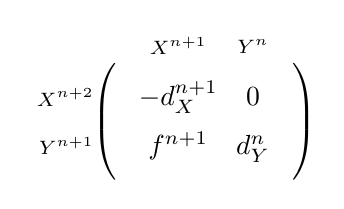
\begin{tikzpicture}[baseline]
			\matrix (M) [matrix of math nodes, ampersand replacement=\&, left delimiter=(, right delimiter=)] {
					-d_X^{n+1} \& 0 \\
					f^{n+1} \& d_Y^n \\
				};
				\node[above=1.2em] at (M-1-1) {\scriptsize $X^{n+1}$};
				\node[above=1.2em] at (M-1-2) {\scriptsize $Y^n$};
				\node[left=2.7em] at (M-1-1) {\scriptsize $X^{n+2}$};
				\node[left=2.7em] at (M-2-1) {\scriptsize $Y^{n+1}$};
		\end{tikzpicture} \\
		& : X^{n+1} \oplus Y^n \to X^{n+2} \oplus Y^{n+1} ,
	\end{align*}
	其中 $n \in \Z$. 由于 $d_{X[1]}^n = -d_X^{n+1}$, 另有简练记法
	\[ \Cone(f) := \left( X[1] \oplus Y , \; \begin{pmatrix} d_{X[1]} & 0 \\ f[1] & d_Y \end{pmatrix} \right) . \]
\end{definition}

易证 $\Cone(f)$ 仍是复形, 这是以下矩阵计算的结论:
\[ \begin{pmatrix} -d_X^{n+1} & 0 \\ f^{n+1} & d_Y^n \end{pmatrix} \begin{pmatrix} -d_X^n & 0 \\ f^n & d_Y^{n-1} \end{pmatrix} =
\begin{pmatrix} d_X^{n+1} d_X^n & 0 \\ - f^{n+1} d_X^n + d_Y^n f^n & d_Y^n d_Y^{n-1} \end{pmatrix}. \]

\begin{example}
	设 $f: X \to Y$ 是 $\mathcal{A}$ 中的态射. 将 $X, Y$ 视同 $\cate{C}(\mathcal{A})$ 的对象 (集中于 $0$ 次项), 则 $\Cone(f)$ 无非是复形 $[X \xrightarrow{f} Y]$ (次数为 $-1, 0$, 其他项全为 $0$).
\end{example}

以下两则函子性按定义是自明的.
\begin{proposition}\label{prop:cone-functorial}
	给定 $\cate{C}(\mathcal{A})$ 中的交换图表
	\[\begin{tikzcd}
		X \arrow[d, "f"'] \arrow[r, "\varphi"] & X' \arrow[d, "{f'}"] \\
		Y \arrow[r, "\psi"'] & Y'
	\end{tikzcd}\]
	则 $\bigl(\begin{smallmatrix} \varphi[1] & 0 \\ 0 & \psi \end{smallmatrix}\bigr)$ 给出态射 $\Cone(f) \to \Cone(f')$.
\end{proposition}

\begin{proposition}\label{prop:Cone-A}
	设 $F: \mathcal{A} \to \mathcal{A}'$ 为加性函子, $f: X \to Y$ 为 $\cate{C}(\mathcal{A})$ 中的态射. 相应的函子 $\cate{C}F: \cate{C}(\mathcal{A}) \to \cate{C}(\mathcal{A}')$ 在 $\cate{C}(\mathcal{A}')$ 中满足典范同构
	\[ (\cate{C}F)(\Cone(f)) \simeq \Cone(\cate{C}F(f)). \]
\end{proposition}

映射锥可以置入以下的``三角'', 这是今后一切理论的基础.
\begin{definition}\label{def:cone-triangle}
	\index[sym1]{alphafbetaf@$\alpha(f), \beta(f)$}
	考虑 $\cate{C}(\mathcal{A})$ 中的态射 $f: X \to Y$. 对之可在 $\cate{C}(\mathcal{A})$ 中构造典范态射
	\[ Y \xrightarrow{\alpha(f)} \Cone(f) \xrightarrow{\beta(f)} X[1] , \]
	具体以矩阵表达如下:
	\begin{align*}
		\alpha(f)^n & := \text{嵌入}\; \begin{pmatrix} 0 \\ \identity_{Y^n} \end{pmatrix}: Y^n \to X[1]^n \oplus Y^n , \\
		\beta(f)^n & := \text{投影}\; \begin{pmatrix} \identity_{X[1]^n} & 0 \end{pmatrix}: X[1]^n \oplus Y^n \to X[1]^n .
	\end{align*}
	易见它们的确给出 $\cate{C}(\mathcal{A})$ 中的态射.
\end{definition}

以下收集关于映射锥的几条同伦性质. 首先我们说明映射锥可以设想为态射的``同伦余核''或``同伦核''. 这是同伦论的基本思想在复形层次的体现.

\begin{proposition}\label{prop:homotopy-kernel-cokernel}
	选定 $\cate{C}(\mathcal{A})$ 中的态射 $f: X \to Y$. 存在典范双射
	\[\begin{tikzcd}[row sep=small]
		\Hom\left( \Cone(f), T \right) \arrow[leftrightarrow, r, "1:1"] & \left\{ (u, h): u \in \Hom(Y,T), \; h: \text{从 $uf$ 到 $0$ 的同伦} \right\}, \\
		\Hom\left( T, \Cone(f)[-1] \right) \arrow[leftrightarrow, r, "1:1"] & \left\{ (v, k): v \in \Hom(T,X), \; k: \text{从 $fv$ 到 $0$ 的同伦} \right\},
	\end{tikzcd}\]
	其中 $T$ 为 $\cate{C}(\mathcal{A})$ 的任意对象, $\Hom := \Hom_{\cate{C}(\mathcal{A})}$. 更具体地说,
	\begin{compactitem}
		\item $\tilde{u}: \Cone(f) \to T$ 的像 $(u, h)$ 满足 $u = \tilde{u} \circ \alpha(f)$,
		\item $\tilde{v}: T \to \Cone(f)[-1]$ 的像 $(v, k)$ 满足 $v = \beta(f)[-1] \circ \tilde{v}$.
	\end{compactitem}
\end{proposition}
\begin{proof}
	首先处理 $\Hom\left( \Cone(f), T \right)$ 的情形. 态射 $\tilde{u}: \Cone(f) \to T$ 相当于一族 $\mathcal{A}$ 中的态射 $h^n: X^{n+1} \to T^n$ 和 $u^n: Y^n \to T^n$, 其中 $n \in \Z$, 所需条件写成矩阵等式
	\[\begin{pmatrix}
		h^{n+1} & u^{n+1}
	\end{pmatrix} \begin{pmatrix}
		-d_X^{n+1} & 0 \\
		f^{n+1} & d_Y^n
	\end{pmatrix} = d_T^n \begin{pmatrix}
		h^n & u^n
	\end{pmatrix}. \]
	具体展开, 可见它相当于说 $u = (u^n)_n: Y \to T$ 是 $\cate{C}(\mathcal{A})$ 中的态射, 而 $h := (h^{n-1})_n$ 满足 $d_{\Hom^\bullet(X, T)}^{-1} h = uf$. 此即所求的双射; 根据 $\alpha(f)$ 的定义, $u = \tilde{u} \circ \alpha(f)$ 是自明的.
	
	其次, 考虑态射 $\tilde{v}: T \to \Cone(f)[-1]$. 这相当于 $\mathcal{A}$ 的态射族 $v^n: T^n \to X^n$ 和 $\underline{k}^n: T^n \to Y^{n-1}$, 所需条件写作
	\[\begin{pmatrix}
		d_X^n & 0 \\
		-f^n & -d_Y^{n-1}
	\end{pmatrix} \begin{pmatrix}
		v^n \\ \underline{k}^n
	\end{pmatrix} = \begin{pmatrix}
		v^{n+1} \\ \underline{k}^{n+1}
	\end{pmatrix} d_T^n
	\quad (n \in \Z). \]
	它相当于说 $v = (v^n)_n: T \to X$ 是 $\cate{C}(\mathcal{A})$ 中的态射, 而 $k := (-\underline{k}^n)_n$ 满足 $d_{\Hom^\bullet(T, Y)}^{-1} k = fv$. 根据 $\beta(f)$ 的定义, $v = \beta(f)[-1] \circ \tilde{v}$ 亦属显然.
\end{proof}

\begin{remark}[同伦余核, 同伦核]\label{rem:homotopy-kernel-cokernel}
	\index{tonglunyuhe@同伦余核, 同伦核 (homotopy cokernel, homotopy kernel)}
	由命题 \ref{prop:homotopy-kernel-cokernel} 推得: 态射 $u: Y \to T$ (或 $v: T \to X$) 满足 $uf$ (或 $fv$) 零伦当且仅当它通过 $\alpha(f): Y \to \Cone(f)$ (或 $\beta(f)[-1]: \Cone(f)[-1] \to X$) 分解. 这自然让人联想到余核 (或核) 的泛性质, 差别在于:
	\begin{compactitem}
		\item 此处以 $uf$ (或 $fv$) 零伦 来替代精确等式 $= 0$;
		\item 命题给出的分解 $\tilde{u}$ (或 $\tilde{v}$) 不仅坐实了 $uf$ (或 $fv$) 零伦这一事实, 还包含了它如何同伦于 $0$, 这是更高一阶的资料.
	\end{compactitem}
	这些性质无法简单地在 $\cate{C}(\mathcal{A})$ 或 $\cate{K}(\mathcal{A})$ 中按照初等范畴论的概念来处理; 实际上 $\cate{K}(\mathcal{A})$ 中鲜少有核或余核. 基于此, $Y \to \Cone(f)$ 又称 $f$ 的\emph{同伦余核}, 而 $\beta(f)[-1]: \Cone(f)[-1] \to X$ 又称 $f$ 的\emph{同伦核}. 耐人寻味的是映射锥 $\Cone(f)$ 及其平移在此意义下兼具``余核''以及``核''两种角色.
\end{remark}

称 $\cate{C}(\mathcal{A})$ 中的态射 $f$ 典范地同伦于 $g$, 如果存在典范的 $h$ 使得 $g -f = d^{-1} h$; 若 $f$ 典范地同伦于 $0$, 则称它典范地零伦.

\begin{proposition}\label{prop:cone-homotopy}
	选定加性范畴 $\mathcal{A}$.
	\begin{enumerate}[(i)]
		\item 若 $f: X \to Y$ 是 $\cate{C}(\mathcal{A})$ 中的同构, 则 $\identity_{\Cone(f)}$ 典范地零伦.
		\item 对于 $\cate{C}(\mathcal{A})$ 中的任意态射 $f: X \to Y$, 定义 \ref{def:cone-triangle} 的态射满足于
		\[ \beta(f) \circ \alpha(f) = 0, \]
		而 $\alpha(f) \circ f$ 和 $f[1] \circ \beta(f)$ 皆典范地零伦.
	\end{enumerate}
\end{proposition}
\begin{proof}
	首先考虑 (i). 基于映射锥的函子性 (命题 \ref{prop:cone-functorial}), 不妨设 $f = \identity_X$. 定义
	\[ s^n := \begin{pmatrix} 0 & \identity_{X^n} \\ 0 & 0 \end{pmatrix} : X^{n+1} \oplus X^n \to X^n \oplus X^{n-1}, \quad n \in \Z. \]
	直接计算给出
	\begin{multline*}
		d^{n-1}_{\Cone(\identity_X)} s^n + s^{n+1} d^n_{\Cone(\identity_X)} = \\
		\begin{pmatrix} -d_X^n & 0 \\ \identity_{X^n} & d_X^{n-1} \end{pmatrix} \begin{pmatrix} 0 & \identity_{X^n} \\ 0 & 0 \end{pmatrix}  + \begin{pmatrix} 0 & \identity_{X^{n+1}} \\ 0 & 0 \end{pmatrix} \begin{pmatrix} -d_X^{n+1} & 0 \\ \identity_{X^{n+1}} & d_X^n \end{pmatrix}
		= \identity_{X^{n+1} \oplus X^n},
	\end{multline*}
	故 $s = (s^n)_{n \in \Z}$ 使 $\identity_{\Cone(\identity_X)}$ 零伦.
	
	接着考虑 (ii). 易见 $\beta(f) \circ \alpha(f) = 0$. 剩下的同伦来自命题 \ref{prop:homotopy-kernel-cokernel}: 取 $T = \Cone(f)$, 则 $\tilde{u} := \identity_{\Cone(f)} \in \Hom(\Cone(f), T)$ 使 $\alpha(f) \circ f$ 零伦; 取 $T = \Cone(f)[-1]$, 则 $\tilde{v} := \identity_{\Cone(f)[-1]} \in \Hom(T, \Cone(f)[-1])$ 使 $f \circ \beta(f)[-1]$ 零伦, 也使 $f[1] \circ \beta(f)$ 零伦.
\end{proof}

定义 \ref{def:cone-triangle} 自 $f$ 引出两个新态射 $\alpha(f)$ 和 $\beta(f)$. 精确到同伦, 它们的映射锥并不产生新对象; 且从 $\Cone(\alpha(f))$ 入手来说明这点. 首先观察到
\[ \Cone(\alpha(f))^n = Y^{n+1} \oplus \Cone(f)^n = Y^{n+1} \oplus X^{n+1} \oplus Y^n. \]
按矩阵写法,
\begin{align*}
	\alpha(\alpha(f)) & = \begin{pmatrix}
		0 & 0 \\
		\identity_{X[1]} & 0 \\
		0 & \identity_Y
	\end{pmatrix} : \Cone(f) \to \Cone(\alpha(f)) , \\
	\beta(\alpha(f)) & = \begin{pmatrix}
		\identity_{Y[1]} & 0 & 0
	\end{pmatrix} : \Cone(\alpha(f)) \to Y[1].
\end{align*}

\begin{lemma}\label{prop:cone-alpha}
	对于 $\cate{C}(\mathcal{A})$ 中的态射 $f: X \to Y$, 用矩阵写法可定义一对态射
	\[ \begin{pmatrix} -f[1] \\ \identity_{X[1]} \\ 0 \end{pmatrix} : \begin{tikzcd} X[1] \arrow[r, shift left, "\phi"] & \Cone(\alpha(f)) \arrow[l, shift left, "\psi"] \end{tikzcd} : \begin{pmatrix} 0 & \identity_{X[1]} & 0 \end{pmatrix}. \]
	它们满足 $\psi \circ \phi = \identity_{X[1]}$, 使下图在 $\cate{K}(\mathcal{A})$ 中交换
	\[\begin{tikzcd}
		\Cone(f) \arrow[d, "{\identity_{\Cone(f)}}"'] \arrow[r, "\beta(f)"] & X[1] \arrow[d, "\phi"] \arrow[r, "{-f[1]}"] & Y[1] \arrow[d, "{\identity_{Y[1]}}"] \\
		\Cone(f) \arrow[r, "{\alpha(\alpha(f))}"'] & \Cone(\alpha(f)) \arrow[r, "\beta(\alpha(f))"'] & Y[1]
	\end{tikzcd}\]
	而且 $\phi, \psi$ 在 $\cate{K}(\mathcal{A})$ 中互逆.
\end{lemma}
\begin{proof}
	根据之前对 $\Cone(\alpha(f))$ 的描述, $d_{\Cone(\alpha(f))}^n$ 按矩阵写法表作
	\[ \begin{pmatrix} -d_Y^{n+1} & 0 & 0 \\ 0 & -d_X^{n+1} & 0 \\ \identity_{Y^{n+1}} & f^{n+1} & d_Y^n \end{pmatrix} : Y^{n+1} \oplus X^{n+1} \oplus Y^n \to Y^{n+2} \oplus X^{n+2} \oplus Y^{n+1}. \]
	问题化为在 $\cate{C}(\mathcal{A})$ 中验证以下断言:
	\begin{itemize}
		\item $\phi := (\phi^n)_{n \in \Z}$ 和 $\psi := (\psi^n)_{n \in \Z}$ 都是复形之间的态射;
		\item $\psi \circ \phi = \identity_{X[1]}$;
		\item $\psi \circ \alpha(\alpha(f)) = \beta(f)$;
		\item $\beta(\alpha(f)) \circ \phi = -f[1]$;
		\item 存在 $s = (s^n)_{n \in \Z} \in \Hom^{-1}\left(\Cone(\alpha(f)), \Cone(\alpha(f))\right)$ 使得 $\identity_{\Cone(\alpha(f))} - \phi \circ \psi = d^{-1}_{\Hom^\bullet} (s)$.
	\end{itemize}
	前四条都是初等的. 以矩阵写法取
	\[ s^n := \begin{pmatrix} 0 & 0 & \identity_{Y^n} \\ 0 & 0 & 0 \\ 0 & 0 & 0 \end{pmatrix}: \Cone(\alpha(f))^n \to \Cone(\alpha(f))^{n-1} \]
	则可验证最后一条断言.
\end{proof}

至于 $\beta(f)$ 的情形, 我们稍事修改, 考虑 $-\beta(f)[-1]: \Cone(f)[-1] \to X$ 的映射锥.
\begin{definition}\label{def:Cyl}
	\index{yingshezhu@映射柱 (mapping cylinder)}
	\index[sym1]{Cylf@$\Cyl(f)$}
	对于 $\cate{C}(\mathcal{A})$ 中的态射 $f: X \to Y$, 其\emph{映射柱}定为
	\[ \Cyl(f) := \Cone\left( \Cone(f)[-1] \xrightarrow{-\beta(f)[-1]} X \right). \]
	它带有典范态射 $X \to \Cyl(f) \to \Cone(f)$.
\end{definition}

映射柱有和映射锥相同形式的函子性 (命题 \ref{prop:cone-functorial}). 鉴于注记 \ref{rem:homotopy-kernel-cokernel}, $\Cyl(f)$ 可与加性范畴中的余像相比拟 --- 它近乎``核的余核'' (命题 \ref{prop:Im-Coim-additive}), 因此也可以视作 $f$ 的同伦余像.

具体地说, $\Cyl(f)^n = \Cone(f)^n \oplus X^n = X^{n+1} \oplus Y^n \oplus X^n$, 态射 $X \to \mathrm{Cyl}(f)$ (或 $\mathrm{Cyl}(f) \to \Cone(f)$) 是向第三个直和项的嵌入 (或向前两个直和项的投影), 而
\[ d_{\Cyl(f)}^n =
	\begin{pmatrix} d_{\Cone(f)}^n & 0 \\ -\beta(f)^n & d_X^n \end{pmatrix}
	= \begin{pmatrix}
		-d_X^{n+1} & 0 & 0 \\
		f^{n+1} & d_Y^n & 0 \\
		-\identity_{X^{n+1}} & 0 & d_X^n
\end{pmatrix} .\]

\begin{lemma}\label{prop:cone-beta}
	对于 $\cate{C}(\mathcal{A})$ 中的态射 $f: X \to Y$, 可定义一对态射
	\[ \begin{pmatrix} 0 \\ \identity_Y \\ 0 \end{pmatrix} : \begin{tikzcd} Y \arrow[r, shift left, "\phi"] & \Cyl(f) \arrow[l, shift left, "\psi"] \end{tikzcd} : \begin{pmatrix} 0 & \identity_Y & f \end{pmatrix}. \]
	它们满足 $\psi \circ \phi = \identity_Y$, 使下图在 $\cate{K}(\mathcal{A})$ 中交换
	\[\begin{tikzcd}
		X \arrow[d, "{\identity_X}"'] \arrow[r, "f"] & Y \arrow[d, "\phi"] \arrow[r, "{\alpha(f)}"] & \Cone(f) \arrow[d, "{\identity_{\Cone(f)}}"] \\
		X \arrow[r] & \Cyl(f) \arrow[r] & \Cone(f)
	\end{tikzcd}\]
	而且 $\phi, \psi$ 在 $\cate{K}(\mathcal{A})$ 中互逆. 进一步, $f$ 分解为 $X \to \Cyl(f) \xrightarrow{\psi} Y$ 的合成.
\end{lemma}
\begin{proof}
	请读者直接按定义验证 $\phi$ 和 $\psi$ 确实给出复形的态射. 只要确立这点, 则 $\psi \circ \phi = \identity_Y$ 一望可知. 接着证 $\phi$ 和 $\psi$ 在 $\cate{K}(\mathcal{A})$ 中互逆: 类似于引理 \ref{prop:cone-alpha}, 取
	\begin{align*}
		s^n & := \begin{pmatrix} 0 & 0 & -\identity_{X^n} \\ 0 & 0 & 0 \\ 0 & 0 & 0 \end{pmatrix}: X^{n+1} \oplus Y^n \oplus X^n \to X^n \oplus Y^{n-1} \oplus X^{n-1}, \\
		s & := (s^n)_{n \in \Z},
	\end{align*}
	并且验证 $\identity_{\Cyl(f)} - \phi \circ \psi = d^{-1}_{\Hom^\bullet} (s)$ 即可.
	
	图表右侧方块在 $\cate{C}(\mathcal{A})$ 中已经交换. 至于左侧方块, 简单观察到 $X \to \mathrm{Cyl}(f) \xrightarrow{\psi} Y$ 合成为 $f$ 便是.
\end{proof}

引理 \ref{prop:cone-alpha} 连同引理 \ref{prop:cone-beta} 表明: 精确到 $\cate{K}(\mathcal{A})$ 中的同构, 任何态射 $f: X \to Y$ 皆能被一个简单得多的投影 $\Cone(\alpha(f))[-1] \to Y$ (或嵌入 $X \to \Cyl(f)$) 来替换, 而且此构造对 $f$ 具函子性. 这在同调代数或同伦论中是一个重要思想.

映射柱在 $f = \identity_X$ 的特例另有妙用, 它可以用来诠释同伦. 对于熟悉同调论的读者, 一切自有拓扑诠释, 但此处只论其代数版本.

\begin{proposition}\label{prop:cylinder-homotopy}
	\index[sym1]{CylX@$\Cyl_X$}
	设 $X$ 为 $\cate{C}(\mathcal{A})$ 的对象, 命 $\mathrm{Cyl}_X := \mathrm{Cyl}(\identity_X)$. 注意到 $\mathrm{Cyl}_X^n = X^{n+1} \oplus X^n \oplus X^n$.
	\begin{enumerate}[(i)]
		\item 在 $\cate{C}(\mathcal{A})$ 中有态射
		$\begin{tikzcd}
			X \arrow[shift left, r, "i_0"] \arrow[shift right, r, "i_1"'] & \Cyl_X \arrow[r, "j"] & X
		\end{tikzcd}$,
		以矩阵记法对每个 $n \in \Z$ 定义为
		\begin{equation*}
			i_0^n := \begin{pmatrix} 0 \\ 0 \\ \identity_{X^n} \end{pmatrix} , \quad
			i_1^n := \begin{pmatrix} 0 \\ \identity_{X^n} \\ 0 \end{pmatrix} , \quad j^n := \begin{pmatrix} 0 & \identity_{X^n} & \identity_{X^n} \end{pmatrix},
		\end{equation*}
		它们满足 $j i_0 = \identity_X = j i_1$, 而且 $j$ 在 $\cate{K}(\mathcal{A})$ 中的像是同构.
		\item 对 $\cate{C}(\mathcal{A})$ 的任意对象 $Y$, 我们有双射
		\begin{align*}
			\left\{\begin{array}{r|l}
				(f, g, h) & f, g \in \Hom_{\cate{C}(\mathcal{A})}(X, Y) \\
				& h \in \Hom^{-1}(X, Y) \\
				& g - f = d^{-1}_{\Hom^\bullet(X, Y)} h
			\end{array}\right\} & \xrightarrow{1:1} \Hom_{\cate{C}(\mathcal{A})}\left( \mathrm{Cyl}_X, Y \right) \\
			(f, g, h) & \longmapsto \tilde{h} = (\tilde{h}^n)_{n \in \Z}, \; \tilde{h}^n := \begin{pmatrix} h^n & g^n & f^n \end{pmatrix}.
		\end{align*}
		特别地, $f = \tilde{h} i_0$ 而 $g = \tilde{h} i_1$.
	\end{enumerate}
\end{proposition}
\begin{proof}
	对于 (i), 注意到 $i_0$ 无非是定义 \ref{def:Cyl} 中的典范态射 $X \to \mathrm{Cyl}(\identity_X)$, 另一方面 $i_1$ 则是引理 \ref{prop:cone-beta} 中的态射 $\phi: X \to \mathrm{Cyl}(\identity_X)$; 引理 \ref{prop:cone-beta} 的交换图表蕴涵两者在 $\cate{K}(\mathcal{A})$ 中给出同一个同构.
	
	至于 $j$, 容易验证 $j^{n+1} d_{\Cyl_X}^n = \bigl(0 \; d_X^n \; d_X^n \bigr) = d_X^n j^n$. 因此 $j$ 确实是态射, 而 $j i_0 = \identity_X = j i_1$ 是自明的. 既然 $i_0$ 和 $i_1$ 在 $\cate{K}(\mathcal{A})$ 中是同构, $j$ 亦然.

	对于 (ii), 将 $\Hom^0(\mathrm{Cyl}_X, Y)$ 的任意元素 $\tilde{h}$ 表作 $\left((h^n, g^n, f^n)\right)_{n \in \Z}$, 其中
	\[ h^n: X^{n+1} \to Y^n, \quad f^n: X^n \to Y^n, \quad g^n: X^n \to Y^n \]
	都是 $\mathcal{A}$ 的态射. 省略上标并以矩阵记法来计算
	\begin{align*}
		\tilde{h} \; d_{\mathrm{Cyl}_X} & = \begin{pmatrix} h & g & f \end{pmatrix} \begin{pmatrix} -d_X & 0 & 0 \\ \identity_X & d_X & 0 \\ -\identity_X & 0 & d_X \end{pmatrix} = \begin{pmatrix} -hd_X + g - f & g d_X & f d_X \end{pmatrix} , \\
		d_Y \; \tilde{h} & = \begin{pmatrix} d_Y h & d_Y g & d_Y f \end{pmatrix}.
	\end{align*}
	因此 $\tilde{h}$ 是复形的态射当且仅当 $f, g \in \Hom_{\cate{C}(\mathcal{A})}(X, Y)$ 而 $g-f = h d_X + d_Y h$.
\end{proof}

\begin{remark}\label{rem:cone-chain}
	\index{yingshezhui}\index{yingshezhu}
	映射锥和映射柱当然有同调版本 (见注记 \ref{rem:cochain-vs-chain}): 给定链复形的态射 $f: X \to Y$, 取
	\[\begin{array}{rlrl}
		\Cone(f)_n & :=(X[-1] \oplus Y)_n, &
		\Cyl(f)_n & := (X[-1] \oplus Y \oplus X)_n, \\
		d_{\Cone(f)} & := \begin{pmatrix} d_{X[-1]} & 0 \\ f[-1] & d_Y \end{pmatrix}, &
		d_{\Cyl(f)} & := \begin{pmatrix} d_{X[-1]} & 0 & 0 \\ f[-1] & d_Y & 0 \\ -\identity_{X[-1]} & 0 & d_X \end{pmatrix}.
	\end{array}\]

	本节所有陈述都能移植到链复形的情形, 特别地, 存在典范态射
	\[ X \xrightarrow{f} Y \xrightarrow{\alpha(f)} \Cone(f) \xrightarrow{\beta(f)} X[-1], \quad X \to \Cyl(f) \to \Cone(f). \]
\end{remark}

\section{相反范畴上的复形}\label{sec:opposite-cplx}
选定加性范畴 $\mathcal{A}$. 本节旨在沟通 $\mathcal{A}$ 和 $\mathcal{A}^{\opp}$ 上的复形. 由于涉及 $\mathcal{A}^{\opp}$ 的函子经常出现, 譬如 $\Hom$ 函子, 这一工序尽管简单却是必要的, 而其中涉及的一些正负号也需要适度的留意. 建议初学的读者略过本节, 或者先大致地浏览.

以下内容分成三个面向: 复形, 同伦, 映射锥. 尔后将探讨的导出范畴版本 (命题 \ref{prop:derived-cat-op}) 是这些结果的直接应用. 回忆到若 $f: X \to Y$ 是 $\mathcal{A}$ 中的态射, 则 $f^{\opp}$ 代表 $\mathcal{A}^{\opp}$ 中对应的态射 $Y \to X$.

\begin{definition-proposition}\label{def:sigma}
	\index[sym1]{sigma@$\sigma$}
	加性范畴的同构 $\sigma: \cate{C}(\mathcal{A}^{\opp}) \to \cate{C}(\mathcal{A})^{\opp}$ 定义如下: 对于 $\cate{C}(\mathcal{A}^{\opp})$ 的对象 $X$, 在 $\mathcal{A}$ 中定义
	\[ (\sigma X)^n := X^{-n}, \quad d_{\sigma X}^n = (-1)^{n+1} \left[ d_X^{-n-1, \opp}: (\sigma X)^n \to (\sigma X)^{n+1} \right], \quad n \in \Z. \]
	对于 $\cate{C}(\mathcal{A}^{\opp})$ 的态射 $f = \left( f^n: X^n \to Y^n \right)_n$, 其像 $\sigma f$ 取作 $\cate{C}(\mathcal{A})$ 的态射
	\[ (\sigma f)^n := \left(f^{-n} \right)^{\opp} : (\sigma Y)^n \to (\sigma X)^n, \]
	亦即 $\cate{C}(\mathcal{A})^{\opp}$ 的态射 $\sigma X \to \sigma Y$. 对所有 $m \in \Z$, 存在自然同构
	\[ s_m: \sigma \circ [m] \rightiso [-m] \circ \sigma, \]
	左式的 $[-m]$ 视同从 $\cate{C}(\mathcal{A})^{\opp}$ 到自身的函子 (严格写法应是 $[-m]^{\opp}$).
\end{definition-proposition}
\begin{proof}
	将 $s_m$ 逐步化到 $m=1$ 情形. 定义 $s_1 = (s_{1, X})_X$ 如下. 对每个 $n$, 取
	\begin{equation}\label{eqn:sigma-s}\begin{tikzcd}[row sep=tiny]
		s_{1,X}^n : \sigma(X{[1]})^n = X^{1-n} \arrow[r, "\sim"', "{(-1)^{n-1}}" inner sep=0.6em] & X^{1-n} = (\sigma X){[-1]}^n .
	\end{tikzcd}\end{equation}
	一切归结为 $s_{1, X}^{n+1} d^n_{\sigma(X[1])} = -d_{X[1]}^{-n-1, \opp} = d_X^{-n, \opp} = (-1)^n d_{\sigma X}^{n-1} = d^n_{(\sigma X)[-1]} s_{1,X}^n$.
\end{proof}

由于 $n(n+1) \equiv 0 \pmod{2}$, 函子 $\sigma$ 操作两次返回自身, 故它确实是范畴之间的同构.

\begin{remark}\label{rem:sigma-vs-cohomology}
	当 $\mathcal{A}$ 是 Abel 范畴时, $d_{\sigma X}^\bullet$ 带的正负号并不改变定义 \ref{def:cohomology} 介绍的上同调; 因此 $\Hm^{-n}(\sigma X) \in \Obj(\mathcal{A})$ 对应到 $\Hm^n(X) \in \Obj(\mathcal{A}^{\opp})$.
\end{remark}

接着探讨 $\sigma$ 和同伦的关系.

\begin{proposition}\label{prop:sigma-homotopy}
	以上定义的 $\sigma$ 诱导加性范畴的等价 $\cate{K}(\mathcal{A}^{\opp}) \rightiso \cate{K}(\mathcal{A})^{\opp}$.
\end{proposition}
\begin{proof}
	选定 $\cate{C}(\mathcal{A}^{\opp})$ 的对象 $X, Y$. 对于 $f = (f^k)_k \in \Hom^{-1}_{\cate{C}(\mathcal{A}^{\opp})}(X, Y)$, 用以下词典在 $\mathcal{A}$ 中定义对应的 $\sigma f \in \Hom^{-1}_{\cate{C}(\mathcal{A})}(\sigma Y, \sigma X)$:
	\[\begin{array}{|c|c|c|c|} \hline
		\text{范畴} & \multicolumn{3}{c|}{\text{态射}} \\ \hline
		\mathcal{A}^{\opp} & X^k \xrightarrow{(-1)^{k+1} f^k} Y^{k-1} & d_Y^{k-1} f^k + f^{k+1} d_X^k & (d^{-1}f)^k \\
		\mathcal{A} & (\sigma Y)^{-k+1} \xrightarrow{(\sigma f)^{-k+1}} (\sigma X)^{-k} & (\sigma f)^{-k+1} d_{\sigma Y}^{-k} + d_{\sigma X}^{-k-1} (\sigma f)^{-k} & d^{-1} (\sigma f)^{-k} \\ \hline
	\end{array}\]	
	这便足以说明 $\Hom_{\cate{K}(\mathcal{A}^{\opp})}(X, Y) \rightiso \Hom_{\cate{K}(\mathcal{A})}(\sigma Y, \sigma X) = \Hom_{\cate{K}(\mathcal{A})^{\opp}}(\sigma X, \sigma Y)$.
\end{proof}

最后, 我们通过之前构造的 $\sigma$ 和同构族 $(s_m)_m$ 来比较 $\cate{C}(\mathcal{A})$ 和 $\cate{C}(\mathcal{A}^{\opp})$ 的映射锥. 这部分的细节是比较琐碎的.

\begin{proposition}\label{prop:sigma-triangulated}
	\index[sym1]{sigma}
	对于 $\cate{C}(\mathcal{A}^{\opp})$ 中的任意态射 $f: X \to Y$, 在 $\cate{C}(\mathcal{A})$ 中\footnote{此处的 $\alpha(\cdot)$ 和 $\beta(\cdot)$ 都是相对于 $\cate{C}(\mathcal{A})$ 来定义的. 若在 $\cate{C}(\mathcal{A})^{\opp}$ 中考量, 则图表的箭头须倒转.}有交换图表
	\[\begin{tikzcd}[column sep=large]
		\sigma\left( X{[1]} \right) \arrow[r, "{\sigma(\beta(f))}"] \arrow[d, "{s_{1,X}}"'] & \sigma\left(\Cone(f)\right) \arrow[r, "{\sigma(\alpha(f))}"] \arrow[d, "\theta"] & \sigma Y \arrow[r, "\sigma(f)"] \arrow[d, "\identity"] & \sigma X \arrow[d, "{\identity}"] \\
		(\sigma X){[-1]} \arrow[r, "{\alpha(\sigma(f))[-1]}"' inner sep=0.6em] & \Cone(\sigma(f)){[-1]} \arrow[r, "{\beta(\sigma(f))[-1]}"' inner sep=0.6em] & \sigma Y \arrow[r, "{\sigma(f)}"' inner sep=0.6em] & \sigma X
	\end{tikzcd}\]
	其中 $\theta$ 是一个典范同构, 而 $s_{1,X}$ 是定义--命题 \ref{def:sigma} 给出的同构.
\end{proposition}
\begin{proof}
	倘若将 $\Cone(f)$ 换作 $X[1] \oplus Y$, 断言则是容易的, 所求同构取 $(s_{1, X}, \identity_{\sigma Y})$ 即可. 这里的麻烦在于 $d_{\Cone(f)}$ 的矩阵有非对角项 $f[1]$. 尽管如此, 我们还是循相同方法, 以 \eqref{eqn:sigma-s} 来对每个 $n \in \Z$ 定义同构
	\begin{multline*}
		\theta^n: \sigma\left(\Cone(f)\right)^n = \sigma\left(X[1]\right)^n \oplus (\sigma Y)^n \\
		\xrightarrow[\sim]{(s_{1,X}, \identity)^n = ((-1)^{n-1} \identity, \identity) } (\sigma X)[-1]^n \oplus (\sigma Y)^n \xlongequal{\text{换位}} \left( (\sigma Y) \oplus (\sigma X)[-1] \right)^n ,
	\end{multline*}	
	而 $\mathcal{A}$ 的态射 $d_{\sigma(\Cone(f))}^n$ 按此对应到
	\[ \begin{pmatrix}
		d_{\sigma Y}^n & 0 \\
		* & d_{(\sigma X)[-1]}^n
	\end{pmatrix} : \left( (\sigma Y) \oplus (\sigma X)[-1] \right)^n \to \left( (\sigma Y) \oplus (\sigma X)[-1] \right)^{n+1} . \]
	如证明开头所述, 对角项不成问题, 重点在于确定矩阵的左下角元素. 基于定义--命题 \ref{def:sigma}, 它等于 $(-1)^{n+1}$ 乘以 $\mathcal{A}$ 中的合成态射
	\[\begin{tikzcd}[row sep=tiny]
		(\sigma Y)^n \arrow[r] & (\sigma(X[1]))^{n+1} \arrow[r, "\sim"] & (\sigma X)[-1]^{n+1} \\
		Y^{-n} \arrow[equal, u] \arrow[r, "{(f^{-n})^{\opp}}"'] & X^{-n} \arrow[equal, u] \arrow[r, "{s_{1, X}^{n+1} = (-1)^n}"'] & X^{-n} \arrow[equal, u]
	\end{tikzcd}\]
	的产物, 亦即 $-\sigma(f)^n$. 由此可见
	\[ \theta := (\theta^n)_{n \in \Z}: \sigma(\Cone(f)) \rightiso \Cone(\sigma(f))[-1] \]
	确实是 $\cate{C}(\mathcal{A})$ 中的同构. 一旦确立这点, 交换性的验证便没有本质困难.
\end{proof}

毋庸赘言, 本节的结果也适用于链复形, 并且可以推广到 $\mathcal{A}$ 为 $\Bbbk$-线性的情形.

\section{双复形}\label{sec:double-cplx}
本节依然取 $\mathcal{A}$ 为加性范畴. 约略地说, 双复形可以设想为复形的二维版本, 带有纵, 横两个方向的微分态射.

\begin{definition}[双复形]\label{def:double-cplx}
	\index{shuangfuxing@双复形 (double complex)}
	\index[sym1]{dhoridvert@$\dhori$, $\dvert$}
	加性范畴 $\mathcal{A}$ 上的双复形意谓 $\mathcal{A}$ 中的一族对象 $\left( X^{p, q} \right)_{(p, q) \in \Z^2}$, 连同态射 $\dhori^{p, q}: X^{p, q} \to X^{p+1, q}$ 和 $\dvert^{p, q}: X^{p, q} \to X^{p, q+1}$, 满足于
	\[ \dhori^{p+1,q} \dhori^{p,q} = 0, \quad \dvert^{p, q+1} \dvert^{p,q} = 0, \quad \dhori^{p, q+1} \dvert^{p,q} = \dvert^{p+1, q} \dhori^{p,q}. \]
	上述资料照例简记为 $(X^{\bullet, \bullet}, \dhori, \dvert)$, $X^{\bullet, \bullet}$ 或 $X$.
\end{definition}

关于 $\dhori, \dvert$ 的条件可简写为
\[ \dhori^2 = 0, \quad \dvert^2 = 0, \quad \dhori \dvert = \dvert \dhori. \]

\begin{definition}\label{def:bicplx}
	给定加性范畴 $\mathcal{A}$, 从双复形 $X$ 到 $Y$ 的态射意谓一族态射
	\[ f = \left( f^{p,q}: X^{p, q} \to Y^{p, q} \right)_{(p, q) \in \Z^2}, \]
	使得对所有 $p, q$ 都有
	\[ \dhori_Y^{p, q} f^{p, q} = f^{p+1, q} \dhori_X^{p, q}, \quad \dvert_Y^{p, q} f^{p, q} = f^{p, q+1} \dvert_X^{p, q}. \]
	上述关系可以简写为 $\dhori_Y f = f \dhori_X$ 和 $\dvert_Y f = f \dvert_X$.
\end{definition}

一如命题 \ref{prop:additive-cat-cplx} 的情形, 这些定义使 $\mathcal{A}$ 上的所有双复形构成加性范畴 $\cate{C}^2(\mathcal{A})$.
\index[sym1]{C2A@$\cate{C}^2(\mathcal{A})$}

双复形 $X$ 形象地表作
\[\begin{tikzcd}
	& \vdots & \vdots & \\
	\cdots \arrow[r] & X^{p, q+1} \arrow[r] \arrow[u] & X^{p+1, q+1} \arrow[r] \arrow[u] & \cdots \\
	\cdots \arrow[r] & X^{p, q} \arrow[r, "{\dhori^{p,q}}"'] \arrow[u, "{\dvert^{p,q}}"] & X^{p+1, q} \arrow[r] \arrow[u] & \cdots \\
	& \vdots \arrow[u] & \vdots \arrow[u] &
\end{tikzcd}\]
每行 $\left( X^{\bullet, q}, d^{\bullet, q} \right)$ 和每列 $\left( X^{p, \bullet}, d^{p, \bullet} \right)$ 都是复形. 因此双复形可以按列或按行收纳.

\begin{definition}\label{def:bicplx-F1}
	\index[sym1]{F1F2@$F_{\mathrm{I}}, F_{\mathrm{II}}$}
	加性函子 $F_{\mathrm{I}}: \cate{C}^2(\mathcal{A}) \to \cate{C}(\cate{C}(\mathcal{A}))$ 定义如下: 对于双复形 $X$, 取 $(F_{\mathrm{I}} X)^p = X^{p, \bullet}$ 而 $d_{F_{\mathrm{I}} X}^p = \dhori^{p, \bullet}: (F_{\mathrm{I}} X)^p \to (F_{\mathrm{I}} X)^{p+1}$. 类似地, 按 $(F_{\mathrm{II}} X)^q = X^{\bullet, q}$ 和 $d_{F_{\mathrm{II}} X}^q = \dvert^{\bullet, q}$ 定义加性函子 $\cate{C}^2(\mathcal{A}) \to \cate{C}(\cate{C}(\mathcal{A}))$. 此处 $p, q \in \Z$.
\end{definition}

定义 \ref{def:bicplx} 蕴涵 $F_{\mathrm{I}}$, $F_{\mathrm{II}}$ 都是加性范畴之间的同构. 示意如下:
\begin{equation}\label{eqn:bicplx-diagram}\begin{tikzcd}[
		/tikz/execute at end picture={
			\node[rectangle, draw, fit=(NW) (SE), inner xsep=0.5em, inner ysep=0em] {};
		}]
		\vdots & |[alias=NW]| & {} & \\
		(F_{\mathrm{II}} X)^q \arrow[u, "{d^q_{F_{\mathrm{II}} X}}"] \arrow[phantom, r, ":=" description, sloped] & \cdots \arrow[r] & X^{p,q} \arrow[r, "{\dhori^{p,q}}"'] \arrow[u, "{\dvert^{p,q}}"] & \cdots \\
		\vdots \arrow[u] & & {} \arrow[u] & |[alias=SE]| \\
		& \cdots \arrow[r] & (F_{\mathrm{I}} X)^p \arrow[r, "{d^p_{F_{\mathrm{I}} X}}"] \arrow[phantom, u, ":=" description, sloped] & \cdots
\end{tikzcd}\end{equation}

\begin{definition}[全复形]\label{def:total-cplx}
	\index{quanfuxing@全复形 (total complex)}
	\index[sym1]{tot@$\tot_{\oplus}$, $\tot_{\Pi}$, $\tot$}
	设 $\mathcal{A}$ 具有可数余积, 以直和符号 $\bigoplus$ 标记, 而 $X$ 是 $\cate{C}^2(\mathcal{A})$ 的对象. 定义 $\mathcal{A}$ 上的复形 $\tot_{\oplus}(X)$ 如下:
	\begin{compactitem}
		\item $\tot_{\oplus}(X)^n := \bigoplus_{p+q=n} X^{p, q}$,
		\item $d^n: \tot_{\oplus}(X)^n \to \tot_{\oplus}(X)^{n+1}$ 拉回到 $X^{p,q}$ 等于 $\dhori^{p,q} + (-1)^p \dvert^{p,q}$.
	\end{compactitem}
\end{definition}

省略上标, 按定义写出 $d^2: X^{p, q} \to X^{p+2, q} \oplus X^{p+1, q+1} \oplus X^{p, q+2}$ 可得
\[ d^2 = \left( \dhori^2, \; (-1)^p \dhori \dvert + (-1)^{p+1} \dvert \dhori , \; \dvert^2 \right) = (0, 0, 0). \]

在函子 $\tot_{\oplus}$ 的构造中以积 $\prod$ 代余积, 可以类似地得到 $\tot_{\Pi} X \in \Obj(\cate{C}(\mathcal{A}))$, 前提是所论的积存在. 此处 $d^n: \tot_{\Pi}(X)^n \to \tot_{\Pi}(X)^{n+1}$ 的定义和 $\tot_{\oplus}$ 情形神似: 我们要求 $d^{n-1}$ 投影到 $X^{p,q}$ 等于
\[ \tot_{\Pi}^{n-1}(X) \xrightarrow{\text{投影}} X^{p-1, q} \oplus X^{p,q-1} \xrightarrow{(\dhori^{p-1, q}, (-1)^p \dvert^{p, q-1})} X^{p, q} \]
的合成; 同理可证 $d^2 = 0$. 不致混淆时, $\tot_{\oplus} X$ 和 $\tot_{\Pi} X$ 都被称为 $X$ 的\emph{全复形}.

以下性质应当是自明的.

\begin{proposition}
	在相应的条件下, $\tot_{\oplus}$ 和 $\tot_{\Pi}$ 都是从 $\cate{C}^2(\mathcal{A})$ 到 $\cate{C}(\mathcal{A})$ 的加性函子.
\end{proposition}

在全复形的定义中, 上标 $p$ 和 $q$ 乍看并不对称. 为了消除这个错觉, 以下来定义 $\cate{C}^2(\mathcal{A})$ 的加性自同构 $\mathrm{swap}$, 使得 $\mathrm{swap}(X)^{p,q} = X^{q, p}$, 并且互换 $\dhori$ 和 $\dvert$. 即将与之搭配的还有符号 $(-1)^{pq}$, 它和 \cite[定义--定理 7.4.4]{Li1} 的 Koszul 符号律本质上是同一套机制.

\index[sym1]{swap@$\mathrm{swap}$}
\begin{proposition}\label{prop:double-cplx-swap}
	对每个 $(p,q) \in \Z^2$ 和 $\cate{C}^2(\mathcal{A})$ 的对象 $X$, 定义一族同构
	\[ r^{p, q}_X := (-1)^{pq} \identity_{X^{p,q}} : X^{p, q} \to \mathrm{swap}(X)^{q,p} . \]
	\begin{compactitem}
		\item 设 $\mathcal{A}$ 有可数余积, 则 $(r_X^{p,q})_{(p,q) \in \Z^2}$ 诱导同构 $r_X: \tot_{\oplus}(X) \rightiso \tot_{\oplus}(\mathrm{swap}(X))$.
		\item 设 $\mathcal{A}$ 有可数积, 则 $(r_X^{p,q})_{(p,q) \in \Z^2}$ 诱导同构 $r_X: \tot_{\Pi}(X) \rightiso \tot_{\Pi}(\mathrm{swap}(X))$.
	\end{compactitem}
\end{proposition}
\begin{proof}
	对所有 $(p,q) \in \Z^2$, 图表
	\[\begin{tikzcd}[row sep=large]
		X^{p,q} \arrow[d, "(-1)^{pq} \identity"'] \arrow[r, "{ (\dhori, (-1)^p \dvert) }" inner sep=0.8em] & X^{p+1, q} \oplus X^{p, q+1} \arrow[d, "{((-1)^{(p+1)q} \identity, (-1)^{p(q+1)} \identity) }"] \\
		X^{p,q} \arrow[r, "{((-1)^q \dhori, \dvert)}"' inner sep=0.8em] & X^{p+1, q} \oplus X^{p, q+1}
	\end{tikzcd}\]
	交换, 故 $r_X$ 确为复形之间的态射.
\end{proof}

在关于 $\tot_{\oplus} X$ (或 $\tot_{\Pi} X$) 的定义中, 可数余积 (或积) 的存在条件可以适当弱化: 如果对所有 $n$, 至多仅有有限个 $(p, q)$ 满足 $p+q=n$ 而 $X^{p,q} \neq 0$, 则全复形定义中的余积 (或积) 化为有限直和. 这时可将两种全复形统一记为 $\tot(X)$. 定义 \ref{def:Cf-Supp} 之后将有进一步的讨论.

\begin{remark}\label{rem:k-fold-cplx}
	准此要领, 对任何 $k \in \Z_{\geq 1}$ 皆可定义 $k$ 重复形为资料
	\[ \left( X^{p_1, \ldots, p_k} \in \Obj(\mathcal{A}) \right)_{p_1, \ldots, p_k \in \Z}, \quad {}^1 d, \ldots, {}^k d, \]
	其中 ${}^i d^{p_1, \ldots, p_k}: X^{p_1, \ldots, p_k} \to X^{p_1, \ldots, p_i + 1, \ldots, p_k}$, 而
	\[ {}^i d^2 = 0, \quad {}^i d {}^j d = {}^j d {}^i d \quad \text{(省略上标)}. \]
	全体 $k$ 重复形构成加性范畴 $\cate{C}^k(\mathcal{A})$. 按定义 \ref{def:bicplx-F1} 的方式还可以定义一族加性函子 $F_i: \cate{C}^k(\mathcal{A}) \to \cate{C}(\cate{C}^{k-1}(\mathcal{A}))$ 使得每个 $F_i$ 都是范畴等价 ($k \geq 2$ 而 $i = 1, \ldots, k$).
	
	在此情形下, 假设 $\mathcal{A}$ 有可数余积或积, 则可依样画葫芦地定义全复形函子
	\[ \tot_{\oplus} \; \text{或} \; \tot_{\Pi}: \cate{C}^k(\mathcal{A}) \to \cate{C}(\mathcal{A}). \]
	细节与双复形的情形无异, 毋须赘述.
\end{remark}

定义从 $\cate{C}^2(\mathcal{A})$ 到自身的同构 $[m]_{\mathrm{I}} := F_{\mathrm{I}}^{-1} \circ [m] \circ F_{\mathrm{I}}$ 和 $[m]_{\mathrm{II}} := F_{\mathrm{II}}^{-1} \circ [m] \circ F_{\mathrm{II}}$, 分别对应到双复形的横向和纵向平移. 对所有 $a, b \in \Z$ 都有 $[a]_{\mathrm{I}} [b]_{\mathrm{II}} = [b]_{\mathrm{II}} [a]_{\mathrm{I}}$. 现在来研究这些函子对全复形的影响, 以及它们和自同构 $\mathrm{swap}$ 的关系.

% Reference: KS06, p.290
\begin{proposition}\label{prop:tot-shift}
	对所有 $X \in \Obj(\cate{C}^2(\mathcal{A}))$ 和 $(p, q) \in \Z^2$, 记标准嵌入 $X^{p, q} \hookrightarrow \mathrm{tot}_{\oplus}(X)^{p+q}$ 为 $\iota_{p, q}$. 对所有 $n \in \Z$, 定义
	\begin{itemize}
		\item $\theta_X^n: \tot_{\oplus} \left( X[1]_{\mathrm{I}} \right)^n \to \tot_{\oplus} \left( X \right)[1]^n$, 使得它拉回到 $X[1]_{\mathrm{I}}^{p, q} = X^{p+1, q}$ 上等于 $\iota_{p+1,q}$;
		\item $(\theta'_X)^n: \tot_{\oplus} \left( X[1]_{\mathrm{II}} \right)^n \to \tot_{\oplus} \left( X \right)[1]^n$, 使得它拉回到 $X[1]_{\mathrm{II}}^{p, q} = X^{p, q+1}$ 上等于 $(-1)^p \iota_{p,q+1}$.
	\end{itemize}
	则它们给出 $\cate{C}(\mathcal{A})$ 中的典范同构
	\begin{align*}
		\theta_X & = (\theta_X^n)_n: \tot_{\oplus} \left( X[1]_{\mathrm{I}} \right) \rightiso \tot_{\oplus} \left(X\right)[1], \\
		\theta'_X & = ((\theta'_X)^n)_n: \tot_{\oplus} \left( X[1]_{\mathrm{II}} \right) \rightiso \tot_{\oplus} \left(X\right)[1],
	\end{align*}
	连同反交换图表 (亦即: 两路合成差一个负号)
	\[\begin{tikzcd}
		\tot_{\oplus} \left( X[1]_{\mathrm{I}}[1]_{\mathrm{II}}\right) \arrow[r, "{\theta_{X[1]_{\mathrm{II}}}}" inner sep=0.6em] \arrow[d, "{\theta'_{X[1]_{\mathrm{I}}}}"'] & \tot_{\oplus}\left(X[1]_{\mathrm{II}}\right)[1] \arrow[d, "{\theta'_X [1]}"] \\
		\tot_{\oplus} \left( X[1]_{\mathrm{I}}\right)[1] \arrow[r, "{\theta_X [1]}"' inner sep=0.6em] & \tot_{\oplus}(X)[2]
	\end{tikzcd}\]
	和交换图表
	\[\begin{tikzcd}[column sep=large]
		\tot_{\oplus} \left( X[1]_{\mathrm{I}}[1]_{\mathrm{II}} \right) \arrow[r, "\text{先 $\theta$ 后 $\theta'$}"] \arrow[d, "{r_{X[1]_{\mathrm{I}}[1]_{\mathrm{II}}}}"'] & \tot_{\oplus}(X)[2] \arrow[d, "{r_X[2]}"] \\
		\tot_{\oplus}\left( \mathrm{swap}(X)[1]_{\mathrm{I}}[1]_{\mathrm{II}} \right) \arrow[r, "\text{先 $\theta'$ 后 $\theta$}"'] & \tot_{\oplus}\left(\mathrm{swap}(X)\right)[2],
	\end{tikzcd}\]
	其中 $r$ 的定义如命题 \ref{prop:double-cplx-swap}. 若以 $\tot_{\Pi}$ 代 $\tot_{\oplus}$, 仍然有同样的 $\theta_X$, $\theta'_X$ 连同相应的反交换图表.
\end{proposition}
\begin{proof}
	直接按全复形的定义 \ref{def:total-cplx} 和平移函子的定义 \ref{def:translation-functor} 来验证 $\theta_X$ 和 $\theta'_X$ 是复形的态射, 细节繁而不难. 反交换图表则归结为如下观察: 图表
	\[\begin{tikzcd}
		X^{p+1, q+1} \arrow[d, "{(-1)^p \identity}"'] \arrow[r, "\identity"] & X^{p+1, q+1} \arrow[d, "{(-1)^{p+1} \identity}"] \\
		X^{p+1, q+1} \arrow[r, "\identity"'] & X^{p+1, q+1}
	\end{tikzcd}\]
	反交换.
	
	现在考虑关于交换图表的断言. 选定 $(p, q) \in \Z^2$, 将两路合成拉回到 $(X[1]_{\mathrm{I}}[1]_{\mathrm{II}})^{p, q}$ 作比较. 先前已说明先 $\theta$ 后 $\theta'$ (对 $X$) 和先 $\theta'$ 后 $\theta$ (对 $\mathrm{swap}(X)$) 分别给出
	\[ (-1)^{p+1}, \; (-1)^q \; \in \Aut(X^{p+1, q+1}) \quad \text{(省略 $\identity$)}. \]
	另一方面, $r_{X[1]_{\mathrm{I}}[1]_{\mathrm{II}}}$ 和 $r_X[2]$ 拉回 $X^{p+1, q+1}$ 分别是 $(-1)^{pq}$ 和 $(-1)^{(p+1)(q+1)}$. 然而 $(p+1)(q+1) - pq \equiv (p+1) - q \pmod{2}$. 明所欲证.
\end{proof}

作为上述反交换图表的简单推广, 请读者证明对于所有 $a, b \in \Z$, 按两种方式定义的
\[ \tot_{\oplus}(X[a]_{\mathrm{I}}[b]_{\mathrm{II}}) \rightrightarrows \tot_{\oplus}(X)[a+b] \]
(先 $\theta$ 后 $\theta'$ 和先 $\theta'$ 后 $\theta$) 相差 $(-1)^{ab}$; 另一方面, 上述交换图表对 $X[a]_{\mathrm{I}} [b]_{\mathrm{II}}$ 仍然成立. 以 $\tot_{\Pi}$ 代 $\tot_{\oplus}$ 亦同.

双复形的主要应用场景之一是关于双函子的研究. 何谓双函子?

\begin{convention}\label{con:bifunctor}
	\index{shuanghanzi@双函子 (bifunctor)}
	形如 $F: \mathcal{A}_1 \times \mathcal{A}_2 \to \mathcal{B}$ 的函子称为\emph{双函子}. 一旦选定对象 $X_i \in \Obj(\mathcal{A}_i)$, 便得到单变元函子 $F(X_1, \cdot): \mathcal{A}_2 \to \mathcal{B}$ 和 $F(\cdot, X_2): \mathcal{A}_1 \to \mathcal{B}$. 由此可以谈论 $F$ 对各个变元的加性, 正合性等诸多概念.
\end{convention}

\begin{definition-proposition}\label{def:bifunctor-cplx}
	\index[sym1]{C2F@$\cate{C}^2 F, \cate{C}_{\oplus} F, \cate{C}_{\Pi} F$}
	设 $\mathcal{A}_1$, $\mathcal{A}_2$, $\mathcal{B}$ 为加性范畴, 而且双函子 $F: \mathcal{A}_1 \times \mathcal{A}_2 \to \mathcal{B}$ 对每个变元都是加性的, 此时有相应的函子
	\[\begin{tikzcd}[row sep=tiny, column sep=small]
		\cate{C}^2 F: \cate{C}(\mathcal{A}_1) \times \cate{C}(\mathcal{A}_2) \arrow[r] & \cate{C}^2(\mathcal{B}) \\
		(X, Y) \arrow[mapsto, r] & (F(X, Y))^{p, q} := F(X^p, Y^q), \\
		& \dhori^{p, q} = F\left( d_X^p, \identity \right), \; \dvert^{p, q} = F\left( \identity, d_Y^q\right) .
	\end{tikzcd}\]

	因此, 在 $\mathcal{B}$ 有可数余积或可数积的前提下, 可分别定义
	\begin{gather*}
		\cate{C}_{\oplus} F := \tot_{\oplus} \circ \cate{C}^2 F: \cate{C}(\mathcal{A}_1) \times \cate{C}(\mathcal{A}_2) \to \cate{C}(\mathcal{B}), \\
		\cate{C}_{\Pi} F := \tot_{\Pi} \circ \cate{C}^2 F: \cate{C}(\mathcal{A}_1) \times \cate{C}(\mathcal{A}_2) \to \cate{C}(\mathcal{B}).
	\end{gather*}
	如果所论的 $\tot_{\oplus}$ 和 $\tot_{\Pi}$ 仅涉及有限直和, 则 $\cate{C}_{\oplus} = \cate{C}_{\Pi}$ 相等.
\end{definition-proposition}
\begin{proof}
	双复形的条件 $\dhori \dvert = \dvert \dhori$ 是双函子定义的直接应用, 其余皆属显然.
\end{proof}

双复形范畴中也有同伦的概念. 设 $f, g: X \to Y$ 是 $\cate{C}^2(\mathcal{A})$ 中的一对态射, 则从 $f$ 到 $g$ 的同伦是指满足以下条件的两族态射 \index{tonglun!双复形版本}
\begin{equation*}\begin{gathered}\begin{tikzcd}
	Y^{p-1, q} & X^{p,q} \arrow[l, "{h^{p,q}}"'] \arrow[d, "{k^{p, q}}"] \\
	& Y^{p, q-1}
\end{tikzcd} \qquad (p,q) \in \Z^2 , \\
	\dvert^{p-1, q} h^{p, q} = h^{p, q+1} \dvert^{p, q}, \qquad \dhori^{p, q-1} k^{p,q} = k^{p+1, q} \dhori^{p,q}, \\
	g^{p,q} - f^{p, q} = \dhori^{p-1, q} h^{p,q} + h^{p+1, q} \dhori^{p,q} + \dvert^{p, q-1} k^{p,q} + k^{p, q+1} \dvert^{p,q}.
\end{gathered}\end{equation*}
这是合理的: 从 $\dvert h = h \dvert$, $\dhori k = k \dhori$ 和双复形的定义, 容易检查 $\dhori h + h \dhori + \dvert k + k \dvert$ 总是给出 $\cate{C}^2(\mathcal{A})$ 的态射.

双复形的同伦反映在全复形上. 详言之, 一旦有 $(h^{p,q}, k^{p,q})_{p,q \in \Z}$, 便可以定义 $\hat{h} \in \Hom^{-1}\left( \tot_{\oplus}(X), \tot_{\oplus}(Y) \right)$, 使 $\hat{h}$ 拉回到直和项 $X^{p,q}$ 上等于
\[ \left( h^{p,q}, (-1)^p k^{p,q} \right): X^{p,q} \to Y^{p-1, q} \oplus Y^{p, q-1}, \]
这将使 $\tot_{\oplus}(g) - \tot_{\oplus}(f) = d^{-1} \hat{h}$; 以相同手法处理 $\tot_{\Pi}$.

综上, 从双复形的同伦关系可以定义 $\cate{K}^2(\mathcal{A})$ 连同函子 $\cate{C}^2(\mathcal{A}) \to \cate{K}^2(\mathcal{A})$, 而在可数余积 (或积) 存在的前提下, 函子 $\tot_{\oplus}$ (或 $\tot_{\Pi}$) 下降为 $\cate{K}^2(\mathcal{A}) \to \cate{K}(\mathcal{A})$. \index[sym1]{K2A@$\cate{K}^2(\mathcal{A})$}

回到加性范畴之间的双函子 $F: \mathcal{A}_1 \times \mathcal{A}_2 \to \mathcal{B}$, 要求它对每个变元都是加性的. 以下是 \eqref{eqn:KF} 的双函子版本.

\begin{proposition}\label{prop:bifunctor-cplx-homotopy}
	\index[sym1]{K2F@$\cate{K}^2 F, \cate{K}_{\oplus} F, \cate{K}_{\Pi} F$}
	取双函子 $F$ 如上, 则 $\cate{C}^2 F$ 分解为 $\cate{K}^2 F: \cate{K}(\mathcal{A}_1) \times \cate{K}(\mathcal{A}_2) \to \cate{K}^2 (\mathcal{B})$.
	
	同理, $\cate{C}_{\oplus} F$ 或 $\cate{C}_{\Pi} F$ 分解为 $\cate{K}(\mathcal{A}_1) \times \cate{K}(\mathcal{A}_2) \to \cate{K}(\mathcal{B})$, 分别记为 $\cate{K}_{\oplus} F$ 或 $\cate{K}_{\Pi} F$, 前提是函子 $\cate{C}_{\oplus} F$ 或 $\cate{C}_{\Pi} F$ 有定义.
\end{proposition}
\begin{proof}
	以 $\cate{C}_{\oplus} F$ 的情形为例, 问题在于对 $\cate{C}(\mathcal{A}_1)$ 的零伦态射 $f_1 = d^{-1} g: X_1 \to Y_1$ 和 $\cate{C}(\mathcal{A}_2)$ 的任意态射 $f_2: X_2 \to Y_2$ 说明对应的 $(\cate{C}^2 F)(f_1, f_2): \cate{C}^2 F(X_1, X_2) \to \cate{C}^2 F(Y_1, Y_2)$ 零伦. 显然的取法是 $h^{p,q} := F(g^p, f_2^q)$ 和 $k^{p,q} := 0$; 因为 $f_2$ 是态射, $h$ 的确与 $\dvert = F(\identity, d)$ 交换. 对第二个变元也类似地处理.
\end{proof}

命题 \ref{prop:tot-shift} 给出典范同构
\begin{gather*}
	\cate{C}_{\oplus} F(X[1], Y) \simeq \cate{C}_{\oplus}F(X, Y)[1] \simeq \cate{C}_{\oplus}(X, Y[1]), \\
	\cate{K}_{\oplus} F(X[1], Y) \simeq \cate{K}_{\oplus}F(X, Y)[1] \simeq \cate{K}_{\oplus}(X, Y[1]).
\end{gather*}
以 $\Pi$ 代 $\oplus$ 亦同.

\begin{example}[$\Hom$ 双复形]\label{eg:Hom-bicplx}
	\index{Hom shuangfuxing@$\Hom$ 双复形 ($\Hom$ double complex)}
	\index[sym1]{Hombb@$\Hom^{\bullet, \bullet}$}
	考虑双函子 $\Hom(\cdot, \cdot): \mathcal{A}^{\opp} \times \mathcal{A} \to \cate{Ab}$, 它映对象 $(S, T)$ 为 $\Hom_{\mathcal{A}}(S, T)$. 以下说明 $\Hom$ 复形 $\Hom^\bullet(X, Y)$ 典范地同构于合成函子
	\[ \cate{C}(\mathcal{A})^{\opp} \times \cate{C}(\mathcal{A}) \xrightarrow{(\sigma^{-1}, \identity)} \cate{C}(\mathcal{A}^{\opp}) \times \cate{C}(\mathcal{A}) \xrightarrow{\cate{C}_{\Pi} \Hom(\cdot, \cdot)} \cate{C}(\cate{Ab}) \]
	在对象 $(X, Y)$ 处的取值, 其中的 $\sigma$ 如定义--命题 \ref{def:sigma}.

	为此, 我们首先考虑从 $\mathcal{A} \times \mathcal{A}^{\opp}$ 到 $\cate{Ab}$ 的双函子 $F(T, S) = \Hom_{\mathcal{A}}(S, T)$, 以及
	\[ \cate{C}(\mathcal{A}) \times \cate{C}(\mathcal{A})^{\opp} \xrightarrow{(\identity, \sigma^{-1})} \cate{C}(\mathcal{A}) \times \cate{C}(\mathcal{A}^{\opp}) \xrightarrow{\cate{C}^2 F} \cate{C}^2(\cate{Ab}). \]
	设 $X, Y \in \Obj(\cate{C}(\mathcal{A}))$. 称对象 $(Y, X)$ 在上述合成函子之下的像 $\Hom^{\bullet, \bullet}(X, Y)$ 为 \emph{$\Hom$ 双复形}. 鉴于显然的交换图表
	\[\begin{tikzcd}[column sep=large]
		\cate{C}(\mathcal{A})^{\opp} \times \cate{C}(\mathcal{A}) \arrow[d, "\simeq"', "\text{对调}"] \arrow[r, "{(\sigma^{-1}, \identity)}" inner sep=0.6em] & \cate{C}(\mathcal{A}^{\opp}) \times \cate{C}(\mathcal{A}) \arrow[r, "{\cate{C}^2 \Hom(\cdot, \cdot)}" inner sep=0.6em] \arrow[d, "\simeq"', "\text{对调}"] & \cate{C}^2(\cate{Ab}) \arrow[d, "\mathrm{swap}"] \\
		\cate{C}(\mathcal{A}) \times \cate{C}(\mathcal{A})^{\opp} \arrow[r, "{(\identity, \sigma^{-1})}"' inner sep=0.6em] & \cate{C}(\mathcal{A}) \times \cate{C}(\mathcal{A}^{\opp}) \arrow[r, "{\cate{C}^2 F}"' inner sep=0.6em] & \cate{C}^2(\cate{Ab})
	\end{tikzcd}\]
	和命题 \ref{prop:double-cplx-swap}, 原问题归结为证 $\tot_{\Pi} \Hom^{\bullet, \bullet}(X, Y)$ 典范地同构于 $\Hom^\bullet(X, Y)$.
	
	细观定义可见
	\begin{equation*}\begin{aligned}
		\Hom^{p, q}(X, Y) & = \Hom_{\mathcal{A}}\left( X^{-q}, Y^p \right), \\
		\dhori^{p, q} & = (d_Y^p)_* : \Hom_{\mathcal{A}}\left( X^{-q}, Y^p \right) \to \Hom_{\mathcal{A}}\left( X^{-q}, Y^{p+1} \right), \\
		\dvert^{p, q} & = (-1)^{q+1} (d_X^{-q-1})^* : \Hom_{\mathcal{A}}\left( X^{-q}, Y^p \right) \to \Hom_{\mathcal{A}}\left( X^{-q-1}, Y^p \right).
	\end{aligned}\end{equation*}
	现在来确定 $\tot_{\Pi} \Hom^{\bullet, \bullet}(X, Y)$. 首先,
	\[ \left(\tot_{\Pi} \Hom^{\bullet, \bullet}(X, Y)\right)^n = \prod_{p+q=n} \Hom_{\mathcal{A}}\left( X^{-q}, Y^p \right) = \prod_{k \in \Z} \Hom\left( X^k, Y^{k+n} \right) \]
	(代入 $k = -q$), 此即 $\Hom^n(X, Y)$. 下一步描述 $d_{\tot_{\Pi} \Hom^{\bullet, \bullet}(X, Y)}^n$: 它在 $\Hom^{n+1}(X, Y)$ 中的第 $(p, q)$ 个坐标 ($p + q = n+1$) 来自
	\[\begin{tikzcd}[column sep=large]
		\Hom^{p-1, q}(X, Y) \arrow[r, "{\dhori^{p-1, q}}"] & \Hom^{p, q}(X, Y) \\
		& \Hom^{p, q-1}(X, Y) \arrow[u, "{(-1)^p \dvert^{p, q-1}}"'] .
	\end{tikzcd}\]
	水平箭头是 $(d_Y^{p-1})_*$, 而垂直箭头是 $(-1)^{p+q} (d_X^{-q})^* = -(-1)^n (d_X^{-q})^*$. 和 $\Hom$ 复形的定义 \ref{def:Hom-cplx} 比较, 立见 $\tot_{\Pi} \Hom^{\bullet, \bullet}(X, Y) = \Hom^\bullet(X, Y)$. 明所欲证.

	最后, 若 $\mathcal{A}$ 是 $\Bbbk$-线性的, 则 $\Hom^{\bullet, \bullet}(X, Y)$ 升级为映至 $\cate{C}^2(\Bbbk\dcate{Mod})$ 的函子.
\end{example}

\section{Abel 范畴上的复形}\label{sec:Abel-cplx}
本节设 $\mathcal{A}$ 为 Abel 范畴. 一如既往, 本节关于加性的陈述都能推广到 $\mathcal{A}$ 为 $\Bbbk$-线性的情形.

对 Abel 范畴上的复形 $X$ 可以探讨上同调 (定义 \ref{def:cohomology}). 回忆到 $[n]$ 不仅平移复形的上标, 还将 $d_X^\bullet$ 乘上符号 $(-1)^n$, 但后者并不改变各个 $d_X$ 的核与像. 由此得到
\[ \Hm^k\left( X[n] \right) = \Hm^{n+k} \left(X \right), \quad k, n \in \Z . \]

命题 \ref{prop:additive-cat-cplx} 已确保 $\cate{C}(\mathcal{A})$ 为加性范畴. 以下说明它还是 Abel 范畴.

\begin{proposition}\label{prop:abelian-cat-cplx}
	范畴 $\cate{C}(\mathcal{A})$ 是 Abel 范畴. 确切地说, 对所有 $X, Y \in \Obj(\cate{C}(\mathcal{A}))$, 我们有 $X \oplus Y = (X^n \oplus Y^n, (d_X^n, d_Y^n))_{n \in \Z}$, 而对于任何态射 $f: X \to Y$, 可取
	\begin{gather*}
		\Ker(f)^n = \left( \Ker(f^n) \right)_{n \in \Z}, \quad \Coker(f)^n = \left( \Coker(f^n) \right)_{n \in \Z}, \\
		\Image(f)^n = \left( \Image(f^n) \right)_{n \in \Z}, \quad \Coim(f)^n = \left( \Coim(f^n) \right)_{n \in \Z}.
	\end{gather*}

	设 $\cate{C}(\mathcal{A})$ 的态射 $f$ 和 $g$ 可合成且 $gf=0$, 则 $H := \Hm\left[ X \xrightarrow{f} Y \xrightarrow{g} Z\right]$ 是以下复形:
	\begin{itemize}
		\item 第 $n$ 次项为 $H^n := \Hm\left[ X^n \xrightarrow{f^n} Y^n \xrightarrow{g^n} Z^n \right]$,
		\item 态射 $d_H^n: H^n \to H^{n+1}$ 由 $d_X^n$, $d_Y^n$ 连同 $\Hm[\cdots]$ 的函子性 (命题 \ref{prop:homology-functoriality}) 确定.
	\end{itemize}
	作为推论, $X \xrightarrow{f} Y \xrightarrow{g} Z$ 正合当且仅当 $X^n \xrightarrow{f^n} Y^n \xrightarrow{g^n} Z^n$ 对每个 $n \in \Z$ 皆正合.
\end{proposition}
\begin{proof}
	命题 \ref{prop:additive-cat-cplx} 业已说明如何以从复形到分次对象的忘却函子 $U: \cate{C}(\mathcal{A}) \to \mathcal{A}^{\Z}$ 将所需的 $\varinjlim$ 和 $\varprojlim$ 逐次地化到 $\mathcal{A}$ 上; 根本在于 $U$ 生 $\varinjlim$ 和 $\varprojlim$ (引理 \ref{prop:limits-cplx}). 这就给出关于 $X \oplus Y$ 和 $\Ker(f)$, $\Coker(f)$ 等等的逐次构造.

	特别地, 根据刻画 \eqref{eqn:strict-morphism}, 典范态射 $\Coim(f) \to \Image(f)$ 由 $\mathcal{A}$ 中的 $\Coim(f^n) \to \Image(f^n)$ 给出. 逐次同构即复形同构. 综上, $\cate{C}(\mathcal{A})$ 的态射皆严格. 故 $\mathcal{A}$ 是 Abel 范畴. 对于 $\Hm[X \to Y \to Z]$ 的描述也是类似处理.
\end{proof}

\begin{remark}
	同理可证双复形范畴 $\cate{C}^2(\mathcal{A})$, 乃至 $k$ 重复形范畴 $\cate{C}^k(\mathcal{A})$ 仍是 Abel 范畴, 其中 $k \in \Z_{\geq 1}$; 见注记 \ref{rem:k-fold-cplx}.
\end{remark}

接着考察 $\cate{C}(\mathcal{A})$ 中的态射 $f: X \to Y$, 命题 \ref{prop:homology-functoriality} 对每个 $n \in \Z$ 唯一地确定 $\Hm^n(f): \Hm^n(X) \to \Hm^n(Y)$, 使得下图交换:
\begin{equation}\label{eqn:induced-morphism-cohomology}\begin{tikzcd}
	\Ker(d_X^n) \arrow[twoheadrightarrow, r] \arrow[d, "\text{由 $f$ 诱导}"'] & \Hm^n(X) \arrow[hookrightarrow, r] \arrow[d, "{\Hm^n(f)}"] & \Coker(d_X^{n-1}) \arrow[d, "\text{由 $f$ 诱导}"] \\
	\Ker(d_Y^n) \arrow[twoheadrightarrow, r] & \Hm^n(Y) \arrow[hookrightarrow, r] & \Coker(d_Y^{n-1}) .
\end{tikzcd}\end{equation}

对给定的态射 $X \xrightarrow{f} Y \xrightarrow{g} Z$, 此刻画即刻给出 $\Hm^n(gf) = \Hm^n(g) \Hm^n(f)$; 此外 $\Hm^n(\identity_X) = \identity_{\Hm^n(X)}$.

\begin{proposition}[上同调作为函子]\label{prop:H-functor}
	\index[sym1]{Hn}
	对所有 $n \in \Z$, 上述定义给出加性函子 $\Hm^n: \cate{C}(\mathcal{A}) \to \mathcal{A}$.
\end{proposition}
\begin{proof}
	性质 $\Hm^n(gf) = \Hm^n(g) \Hm^n(f)$ 和 $\Hm^n(\identity) = \identity$ 直接来自 \eqref{eqn:induced-morphism-cohomology} 的刻画; 同理可得 $\Hm^n(f_1 + f_2) = \Hm^n(f_1) + \Hm^n(f_2)$ 以及 $\Hm^n(tf) = t\Hm^n(f)$, 若 $\mathcal{A}$ 是 $\Bbbk$-线性的而 $t \in \Bbbk$.
\end{proof}

复形之间的短正合列自动诱导上同调的长正合列, 这是长正合列在同调论中最初等的形式.

\begin{proposition}[短正合列诱导长正合列]\label{prop:long-exact-sequence-ses}
	\index{changzhenghelie@长正合列 (long exact sequence)}
	设 $0 \to X \xrightarrow{f} Y \xrightarrow{g} Z \to 0$ 是 $\cate{C}(\mathcal{A})$ 中的短正合列, 则基于定理 \ref{prop:snake-lemma} 可导出 $\mathcal{A}$ 中的典范正合列
	
	\begin{equation*}\begin{tikzcd}[row sep=large]
	\cdots \arrow[r] & \Hm^{n-1}(Y) \arrow[r, "{\Hm^{n-1}(g)}" inner sep=0.7em] \arrow[phantom, d, ""{coordinate, name=A}] & \Hm^{n-1}(Z) \arrow[dll, rounded corners, "{\delta^{n-1}}" description, to path={
		-- ([xshift=2ex]\tikztostart.east)
		|- (A) [near end]\tikztonodes
		-| ([xshift=-2ex]\tikztotarget.west)
		-- (\tikztotarget)}] \\
	\Hm^n(X) \arrow[r, "{\Hm^n(f)}"] & \Hm^n(Y) \arrow[r, "{\Hm^n(g)}"] \arrow[phantom, d, ""{coordinate, name=B}] & \Hm^n(Z) \arrow[dll, rounded corners, "{\delta^n}" description, to path={
		-- ([xshift=2ex]\tikztostart.east)
		|- (B) [near end]\tikztonodes
		-| ([xshift=-2ex]\tikztotarget.west)
		-- (\tikztotarget)}] \\
	\Hm^{n+1}(X) \arrow[r, "{\Hm^{n+1}(f)}"' inner sep=0.7em] & \Hm^{n+1}(Y) \arrow[r] & \cdots
	\end{tikzcd}\end{equation*}
	
	它具备如下的函子性: 若有 $\cate{C}(\mathcal{A})$ 中的行正合交换图表
	\[\begin{tikzcd}[row sep=small]
		0 \arrow[r] & X \arrow[r] \arrow[d] & Y \arrow[r] \arrow[d] & Z \arrow[d] \arrow[r] & 0 \\
		0 \arrow[r] & \underline{X} \arrow[r] & \underline{Y} \arrow[r] & \underline{Z} \arrow[r] & 0
	\end{tikzcd}\]
	则它们给出交换图表
	\[\begin{tikzcd}[column sep=small, row sep=small]
		\cdots \arrow[r] & \Hm^n(X) \arrow[d] \arrow[r] & \Hm^n(Y) \arrow[r] \arrow[d] & \Hm^n(Z) \arrow[r] \arrow[d] & \Hm^{n+1}(X) \arrow[r] \arrow[d] & \cdots \\
		\cdots \arrow[r] & \Hm^n(\underline{X}) \arrow[r] & \Hm^n(\underline{Y}) \arrow[r] & \Hm^n(\underline{Z}) \arrow[r] & \Hm^{n+1}(\underline{X}) \arrow[r] & \cdots .
	\end{tikzcd}\]
\end{proposition}
\begin{proof}
	对每个 $n \in \Z$ 皆有正合列 $\Coker(d_X^n) \to \Coker(d_Y^n) \to \Coker(d_Z^n) \to 0$: 对
	\[\begin{tikzcd}
		0 \arrow[r] & X^{n-1} \arrow[r] \arrow[d] & Y^{n-1} \arrow[r] \arrow[d] & Z^{n-1} \arrow[r] \arrow[d] & 0 \\
		0 \arrow[r] & X^n \arrow[r] & Y^n \arrow[r] & Z^n \arrow[r] & 0
	\end{tikzcd}\]
	取定理 \ref{prop:snake-lemma} 之正合列的 $\Coker$ 部分便是. 类似道理, 也有正合列 $0 \to \Ker(d_X^n) \to \Ker(d_Y^n) \to \Ker(d_Z^n)$. 它们可以置入行正合的交换图表
	\begin{equation}\label{eqn:long-exact-sequence-ses-aux}\begin{tikzcd}
		& \Coker(d_X^{n-2}) \arrow[r] \arrow[d] & \Coker(d_Y^{n-2}) \arrow[r] \arrow[d] & \Coker(d_Z^{n-2}) \arrow[d] \arrow[r] & 0 \\
		0 \arrow[r] & \Ker(d_X^n) \arrow[r] & \Ker(d_Y^n) \arrow[r] & \Ker(d_Z^n) &
	\end{tikzcd}\end{equation}
	垂直箭头分别由 $d_X^{n-1}$, $d_Y^{n-1}$, $d_Z^{n-1}$ 诱导, 具有形如 $\Coker(d^{n-2}) \stackrel{d^{n-1}}{\twoheadrightarrow} \Image(d^{n-1}) \hookrightarrow \Ker(d^n)$ 的满--单分解 (省略下标).
	
	根据引理 \ref{prop:mono-epi-ker-coker} (iii), 可从 $\Coker(d^{n-2}) \twoheadrightarrow \Image(d^{n-1})$ 确定 \eqref{eqn:long-exact-sequence-ses-aux} 中垂直箭头的核, 再由 \eqref{eqn:homology-3} 依序得到 $\Hm^{n-1}(X)$, $\Hm^{n-1}(Y)$, $\Hm^{n-1}(Z)$; 同理, 从 $\Image(d^{n-1}) \hookrightarrow \Ker(d^n)$ 确定垂直箭头的余核, 则依序得到 $\Hm^n(X)$, $\Hm^n(Y)$ 和 $\Hm^n(Z)$. 应用定理 \ref{prop:snake-lemma} 以得出连接态射 $\delta^{n-1}: \Hm^{n-1}(Z) \to \Hm^n(X)$ 和长正合列中涉及 $\Hm^n$ 和 $\Hm^{n-1}$ 的项. 应用注记 \ref{rem:connecting-canonical} 可得函子性.
\end{proof}

\begin{definition}[拟同构]\label{def:quasi-isomorphism}
	\index{nitonggou@拟同构 (quasi-isomorphism)}
	设 $f: X \to Y$ 为 $\cate{C}(\mathcal{A})$ 中的态射. 若 $\Hm^n(f)$ 对所有 $n \in \Z$ 皆为同构, 则称 $f$ 为拟同构.
\end{definition}

\begin{proposition}\label{prop:null-homotopic-cohomology}
	设 $f: X \to Y$ 为 $\cate{C}(\mathcal{A})$ 的态射, $n \in \Z$. 若 $f$ 零伦, 则 $\Hm^n(f) = 0$.
\end{proposition}
\begin{proof}
	取 $h \in \Hom^{-1}(X, Y)$ 使得 $f = d_Y h + h d_X$. 合成态射 $\Ker(d_X^n) \hookrightarrow X^n \xrightarrow{h^{n+1} d_X^n} Y^n$ 为 $0$, 另一方面 $d_Y^{n-1} h^n$ 通过 $\Image(d_Y^{n-1})$ 分解. 两者搭配给出 $\Hm^n(f) = 0$.
\end{proof}

\begin{corollary}
	对所有 $n \in \Z$, 上同调函子 $\Hm^n: \cate{C}(\mathcal{A}) \to \mathcal{A}$ 唯一地通过 $\cate{K}(\mathcal{A})$ 分解. 故拟同构的概念可以扩及 $\cate{K}(\mathcal{A})$ 的态射. 若 $f: X \to Y$ 在 $\cate{K}(\mathcal{A})$ 中为同构, 则 $f$ 是拟同构.
\end{corollary}
\begin{proof}
	结合命题 \ref{prop:homotopy-category-universal-property} 和 \ref{prop:null-homotopic-cohomology}.
\end{proof}


\section{映射锥和长正合列}\label{sec:cone-vs-long-exact-sequence}
长正合列是同调代数的主要工具, 本节旨在比较从短正合列构造长正合列的三种方法. 精确到一些正负号, 它们殊途同归. 以下取 $\mathcal{A}$ 为 Abel 范畴.

\begin{proposition}\label{prop:cone-triangle-ses}
	设 $f: X \to Y$ 为 $\cate{C}(\mathcal{A})$ 中的态射. 令 $\alpha(f)$, $\beta(f)$ 如定义 \ref{def:cone-triangle}, 则
	\[ 0 \to Y \xrightarrow{\alpha(f)} \Cone(f) \xrightarrow{\beta(f)} X[1] \to 0 \]
	是 $\cate{C}(\mathcal{A})$ 中的正合列.
\end{proposition}
\begin{proof}
	回忆 $\alpha(f)$ 和 $\beta(f)$ 的定义. 既然正合性可以逐次检验 (命题 \ref{prop:abelian-cat-cplx}), 断言遂归结为
	\[ 0 \to Y^n \xrightarrow{(0, \identity)} X^{n+1} \oplus Y^n \xrightarrow{\text{投影}} X^{n+1} \to 0, \]
	对每个 $n \in \Z$ 的正合性, 此即命题 \ref{prop:biproduct-ses} 的内容.
\end{proof}

给定 $\cate{C}(\mathcal{A})$ 中的态射 $f: X \to Y$, 命题 \ref{prop:cone-triangle-ses} 的短正合列连同命题 \ref{prop:long-exact-sequence-ses} 给出 $\mathcal{A}$ 中的长正合列
\begin{equation}\label{eqn:cone-long-exact-sequence}
	\cdots \to \Hm^n(Y) \xrightarrow{\Hm^n(\alpha(f))} \Hm^n(\Cone(f)) \xrightarrow{\Hm^n(\beta(f))} \underbracket{\Hm^n(X[1])}_{= \Hm^{n+1}(X)} \xrightarrow{\xi^n} \Hm^{n+1}(Y) \to \cdots
\end{equation}
标为 $\xi^n$ 者是诱导自短正合列的连接态射; 推论 \ref{prop:cone-connecting} 将证明 $\xi^n$ 无非是 $\Hm^{n+1}(f): \Hm^{n+1}(X) \to \Hm^{n+1}(Y)$, 所以映射锥的长正合列 \eqref{eqn:cone-long-exact-sequence} 其每段都是明确的, 都来自 $f$, $\alpha(f)$ 和 $\beta(f)$.

下述结果则从另一个方向表明: 从 $\cate{C}(\mathcal{A})$ 中任意短正合列出发, 也可以自然地和映射锥建立联系. 方式分两种.

\begin{lemma}\label{prop:cone-qis}
	给定 $\cate{C}(\mathcal{A})$ 中的短正合列 $0 \to X \xrightarrow{f} Y \xrightarrow{g} Z \to 0$, 则
	\[ \Phi := (0, g): \Cone(f) \to Z, \quad \Phi' := (f[1], 0): X[1] \to \Cone(g) \]
	皆是复形之间的拟同构, 它们具有以下性质:
	\begin{enumerate}[(i)]
		\item $\Phi \circ \alpha(f) = g$ 而 $\beta(g) \circ \Phi' = f[1]$,
		\item $\alpha(g)\Phi + \Phi'\beta(f): \Cone(f) \to \Cone(g)$ 典范地零伦.
	\end{enumerate}
\end{lemma}
\begin{proof}
	端详 $\cate{C}(\mathcal{A})$ 的交换图表
	\[\begin{tikzcd}[column sep=small]
		0 \arrow[r] & X \arrow[r, "\identity_X"] \arrow[d, "{\identity_X}"'] & X \arrow[r] \arrow[d, "f"] & 0 \arrow[r] \arrow[d] & 0 \\
		0 \arrow[r] & X \arrow[r, "f"'] & Y \arrow[r, "g"'] & Z \arrow[r] & 0
	\end{tikzcd} \quad \begin{tikzcd}[column sep=small]
		0 \arrow[r] & X \arrow[d] \arrow[r, "f"] & Y \arrow[d, "g"'] \arrow[r, "g"] & Z \arrow[d, "\identity_Z"] \arrow[r] & 0 \\
		0 \arrow[r] & 0 \arrow[r] & Z \arrow[r, "\identity_Z"'] & Z \arrow[r] & 0
	\end{tikzcd}\]
	每一行皆正合; 映射锥的函子性 (命题 \ref{prop:cone-functorial}) 遂给出 $\cate{C}(\mathcal{A})$ 中的态射
	\begin{equation}\label{eqn:cone-qis-aux}\begin{tikzcd}[row sep=tiny]
		0 \arrow[r] & \Cone\left( \identity_X \right) \arrow[r] & \Cone\left( X \xrightarrow{f} Y \right) \arrow[r] & \Cone\left( 0 \to Z \right) \arrow[r] & 0 \\
		0 \arrow[r] & \Cone(X \to 0) \arrow[r] & \Cone\left( Y \xrightarrow{g} Z \right) \arrow[r] & \Cone\left( \identity_Z \right) \arrow[r] & 0
	\end{tikzcd}\end{equation}
	逐次考察, 并利用前述交换图表及映射锥的定义, 可见 \eqref{eqn:cone-qis-aux} 每行皆正合. 此外, 容易看出 $\Cone(f) \to \Cone(0 \to Z) \simeq Z$ (或 $X[1] \simeq \Cone(X \to 0) \to \Cone(g)$) 即是 $\Phi$ (或 $\Phi'$). 一旦知道它们是复形的态射, (i) 的等式便是自明的.
	
	对 \eqref{eqn:cone-qis-aux} 应用命题 \ref{prop:long-exact-sequence-ses}, 便对每个 $n \in \Z$ 得到正合列
	\begin{gather*}
		\Hm^n\left( \Cone(\identity_X) \right) \to \Hm^n \left( \Cone(f) \right) \xrightarrow{\Hm^n(\Phi)} \Hm^n(Z) \to \Hm^{n+1} \left( \Cone(\identity_X) \right), \\
		\Hm^{n-1}\left( \Cone(\identity_Z) \right) \to \Hm^n(X[1]) \xrightarrow{\Hm^n(\Phi')} \Hm^n\left( \Cone(g) \right) \to \Hm^n\left( \Cone(\identity_Z) \right).
	\end{gather*}
	引理 \ref{prop:cone-homotopy} (i) 和命题 \ref{prop:null-homotopic-cohomology} 表明左右端点项皆为 $0$, 故 $\Phi$ 和 $\Phi'$ 是拟同构.
	
	最后验证 (ii). 按照 $\Cone(f)^n = X^{n+1} \oplus Y^n$ 和 $\Cone(g)^n = Y^{n+1} \oplus Z^n$ 将态射写成矩阵
	\begin{gather*}\begin{tikzcd}[row sep=tiny, column sep=large, ampersand replacement=\&]
		\& Z \arrow[rd, "\alpha(g)" description, "{\bigl(\begin{smallmatrix} 0 \\ \identity \end{smallmatrix} \bigr)}" inner sep=0.6em] \& \\
		\Cone(f) \arrow[ru, "\Phi" description, "{\bigl( 0 \; g \bigr)}" inner sep=0.6em] \arrow[rd, "\beta(f)" description, "{\big( \identity \; 0 \bigr)}"' inner sep=0.6em] \& \& \Cone(g) \\
		\& X[1] \arrow[ru, "{\Phi'}" description, "{\bigl( \begin{smallmatrix} f[1] \\ 0 \end{smallmatrix} \bigr)}"' inner sep=0.6em] \&
	\end{tikzcd}, \quad
		\alpha(g) \Phi + \Phi' \beta(f) = \begin{pmatrix} f[1] & 0 \\ 0 & g  \end{pmatrix}.
	\end{gather*}
	另外取 $s = (s^n)_n \in \Hom^{-1}\left( \Cone(f), \Cone(g) \right)$ 为
	\[ s^n := \begin{pmatrix}
		0 & \identity_{Y^n} \\
		0 & 0
	\end{pmatrix}: X^{n+1} \oplus Y^n \to Y^n \oplus Z^{n-1} , \]
	这也是唯一合理的取法. 直接的矩阵计算表明 $d_{\Cone(g)}^{n-1} s^n + s^{n+1} d_{\Cone(f)}^n$ 等于
	\[\begin{pmatrix}
		-d_Y^n & 0 \\
		g^n & d_Z^{n-1}
	\end{pmatrix} \begin{pmatrix}
		0 & \identity_{Y^n} \\
		0 & 0
	\end{pmatrix} + \begin{pmatrix}
		0 & \identity_{Y^{n+1}} \\
		0 & 0
	\end{pmatrix} \begin{pmatrix}
		-d_X^{n+1} & 0 \\
		f^{n+1} & d_Y^n
	\end{pmatrix} = \begin{pmatrix}
		f^{n+1} & 0 \\
		0 & g^n
	\end{pmatrix}.\]
	故 $\alpha(g)\Phi + \Phi'\beta(f)$ 确实零伦.
\end{proof}

综上, 从 $\cate{C}(\mathcal{A})$ 中的短正合列 $0 \to X \xrightarrow{f} Y \xrightarrow{g} Z \to 0$ 出发, 有三种方式在 $\mathcal{A}$ 中导出长正合列
\[\begin{tikzcd}[row sep=large]
	\cdots \arrow[r] & \Hm^{n-1}(Y) \arrow[r] \arrow[phantom, d, ""{coordinate, name=A}] & \Hm^{n-1}(Z) \arrow[dll, rounded corners, to path={
		-- ([xshift=2ex]\tikztostart.east)
		|- (A) [near end]\tikztonodes
		-| ([xshift=-2ex]\tikztotarget.west)
		-- (\tikztotarget)}] \\
	\Hm^n(X) \arrow[r] & \Hm^n(Y) \arrow[r] \arrow[phantom, d, ""{coordinate, name=B}] & \Hm^n(Z) \arrow[dll, rounded corners, to path={
		-- ([xshift=2ex]\tikztostart.east)
		|- (B) [near end]\tikztonodes
		-| ([xshift=-2ex]\tikztotarget.west)
		-- (\tikztotarget)}] \\
	\Hm^{n+1}(X) \arrow[r] & \Hm^{n+1}(Y) \arrow[r] & \cdots .
\end{tikzcd}\]
\begin{enumerate}[(A)]
	\item 直接应用命题 \ref{prop:long-exact-sequence-ses} 得到长正合列
	\[\begin{tikzcd}
		\cdots \arrow[r] & \Hm^n(Y) \arrow[r, "{\Hm^n(g)}" inner sep=0.6em] & \Hm^n(Z) \arrow[r, "{\delta^n}" inner sep=0.6em] & \Hm^{n+1}(X) \arrow[r, "{\Hm^{n+1}(f)}" inner sep=0.6em] & \Hm^{n+1}(Y) \arrow[r] & \cdots
	\end{tikzcd}\]
	\item 应用引理 \ref{prop:cone-qis} 的拟同构 $\Phi: \Cone(f) \to Z$, 配合 \eqref{eqn:cone-long-exact-sequence} 得出交换图表
	\[\begin{tikzcd}[column sep=scriptsize]
		\cdots \arrow[r] & \Hm^n(Y) \arrow[r, "{\Hm^n(\alpha(f))}" inner sep=0.6em] \arrow[equal, d] & \Hm^n\left( \Cone(f) \right) \arrow[r, "{\Hm^n(\beta(f))}" inner sep=0.6em] \arrow[d, "{\Hm^n(\Phi)}"] & \Hm^n(X[1]) \arrow[r] \arrow[equal, d] & \Hm^{n+1}(Y) \arrow[r] \arrow[equal, d] & \cdots \\
		\cdots \arrow[r] & \Hm^n(Y) \arrow[r, "{\Hm^n(g)}"' inner sep=0.6em] & \Hm^n(Z) \arrow[r, "{\eta^n}"' inner sep=0.6em] & \Hm^{n+1}(X) \arrow[r, "{\xi^n}"' inner sep=0.6em] & \Hm^{n+1}(Y) \arrow[r] & \cdots
	\end{tikzcd}\]
	其中
	\begin{compactitem}
		\item $\eta^n := \Hm^n(\beta(f)) \Hm^n(\Phi)^{-1}$,
		\item $\xi^n$ 是 \eqref{eqn:cone-long-exact-sequence} 中的连接态射 $\Hm^{n+1}(X) = \Hm^n(X[1]) \to \Hm^{n+1}(Y)$.
	\end{compactitem}
	已知第一行正合, 故第二行亦然.

	\item 同上, 但改用引理 \ref{prop:cone-qis} 的拟同构 $\Phi': X[1] \to \Cone(g)$, 得到交换图表
	\[\begin{tikzcd}[column sep=scriptsize]
		\cdots \arrow[r] & \Hm^n(Z) \arrow[r, "{\Hm^n(\alpha(g))}" inner sep=0.6em] & \Hm^n\left( \Cone(g) \right) \arrow[r, "{\Hm^n(\beta(g))}" inner sep=0.6em] & \Hm^n(Y[1]) \arrow[r] & \Hm^{n+1}(Z) \arrow[r] & \cdots \\
		\cdots \arrow[r] & \Hm^n(Z) \arrow[r, "{(\eta')^n}"' inner sep=0.6em] \arrow[equal, u] & \Hm^n(X[1]) \arrow[r, "{\Hm^n(f[1])}"' inner sep=0.6em] \arrow[u, "{\Hm^n(\Phi')}"', "\simeq"] & \Hm^{n+1}(Y) \arrow[r, "{(\xi')^n}"' inner sep=0.6em] \arrow[equal, u] & \Hm^{n+1}(Z) \arrow[r] \arrow[equal, u] & \cdots
	\end{tikzcd}\]
	其中
	\begin{compactitem}
		\item $(\eta')^n := \Hm^n(\Phi')^{-1} \Hm^n(\alpha(g))$,
		\item $(\xi')^n$ 来自 \eqref{eqn:cone-long-exact-sequence} (以 $g$ 代 $f$) 中的连接态射 $\Hm^{n+1}(Y) = \Hm^n(Y[1]) \to \Hm^{n+1}(Z)$.
	\end{compactitem}
	已知第一行正合, 故第二行亦然.
\end{enumerate}

这三种长正合列有何异同? 我们先来陈述结论.

\begin{itemize}
	\item 构造 (A) 和 (B) 仅差一些负号: 命题 \ref{prop:connecting-eta-delta} 将说明 $\eta^n = -\delta^n$, 而推论 \ref{prop:cone-connecting} 则蕴涵 $\xi^n = \Hm^{n+1}(f)$.
	\item 构造 (A) 和 (C) 的产物相同: 推论 \ref{prop:connecting-eta-delta-2} 将基于 (B) 的结果来说明 $(\eta')^n = \delta^n$, 而推论 \ref{prop:cone-connecting} 蕴涵 $(\xi')^n = \Hm^{n+1}(g)$.
	\item 因此 (B) 和 (C) 仅在连接态射 $\Hm^n(Z) \to \Hm^{n+1}(X)$ 处差一个负号, 这点可由三角范畴的旋转公理 (TR3) 得到解释, 详见之后的命题 \ref{prop:ses-vs-triangle}.
\end{itemize}
接着着手来确立这些关系.

\begin{proposition}\label{prop:connecting-eta-delta}
	在上述场景中, $\eta^n = -\delta^n$ 对所有 $n \in \Z$ 皆成立.
\end{proposition}
\begin{proof}
	以下论证取自 \cite[Proposition 12.3.6]{KS06}. 由于论证比较曲折, 敬邀读者先尝试 $\mathcal{A} = R\dcate{Mod}$ 的具体情形, 其中 $R$ 是环; 图追踪 \cite[\S 6.8]{Li1} 的办法对之给出直截了当的证明.

	对于一般的 Abel 范畴 $\mathcal{A}$, 首先选定 $n \in \Z$, 取纤维积
	\[ S := \Coker(d_Y^{n-1}) \dtimes{\Coker(d_Z^{n-1})} \Hm^n(Z). \]
	连接同态 $\delta^n$ 如何构造? 它是施 \eqref{eqn:snake-conn} 于 \eqref{eqn:long-exact-sequence-ses-aux} 的图表
	\[\begin{tikzcd}
		& \Coker(d_X^{n-1}) \arrow[r] \arrow[d] & \Coker(d_Y^{n-1}) \arrow[r] \arrow[d] & \Coker(d_Z^{n-1}) \arrow[d] \arrow[r] & 0 \\
		0 \arrow[r] & \Ker(d_X^{n+1}) \arrow[r] & \Ker(d_Y^{n+1}) \arrow[r] & \Ker(d_Z^{n+1}) &
	\end{tikzcd}\]
	的产物, 在此调整为
	\begin{equation}\label{eqn:connecting-eta-delta-0}\begin{tikzcd}
		& S \arrow[twoheadrightarrow, r, "w"] \arrow[d, "v"] \arrow[ldd, bend right, "u"'] \arrow[rd, phantom, "\Box" description] & \Hm^n(Z) \arrow[hookrightarrow, d] \\
		& \Coker(d_Y^{n-1}) \arrow[twoheadrightarrow, r] \arrow[d, "a"] & \Coker(d_Z^{n-1}) \arrow[d] \\
		\Ker(d_X^{n+1}) \arrow[hookrightarrow, r, "b"'] \arrow[twoheadrightarrow, d] & \Ker(d_Y^{n+1}) \arrow[r, "c"'] & \Ker(d_Z^{n+1}) \\
		\Hm^{n+1}(X) & &
	\end{tikzcd}\end{equation}
	的形式; 图中行列皆正合, 箭头 $a$ 由 $d_Y^n$ 诱导, $b$ 由 $f^{n+1}$ 诱导, 而箭头 $u$ 的存在性和唯一性是缘于右半部交换蕴涵 $cav = 0$. 细心回顾 \eqref{eqn:snake-conn} 的构造可见图表
	\begin{equation}\label{eqn:connecting-eta-delta-0.5}\begin{tikzcd}[row sep=tiny]
		& \Hm^n(Z) \arrow[rd, "\delta^n"] & \\
		S \arrow[twoheadrightarrow, ru, "w"] \arrow[rd, "u"'] & & \Hm^{n+1}(X) \\
		& \Ker\left( d_X^{n+1} \right) \arrow[twoheadrightarrow, ru] &
	\end{tikzcd} \quad \text{交换}; \end{equation}
	因为 $w$ 已知满, 此图表也唯一地确定了 $\delta^n$.
	
	为了和映射锥作比较, 请按定义验证下图交换
	\[\begin{tikzcd}
		\Ker(d_X^{n+1}) \oplus \Coker(d_Y^{n-1}) \arrow[d, "{(b,a)}"'] \arrow[hookrightarrow, r] & X^{n+1} \oplus \Coker\left( d_Y^{n-1} \right) \arrow[twoheadrightarrow, r] & \Coker\left( d_{\Cone(f)}^{n-1} \right) \arrow[d, "{d_{\Cone(f)}^n}"] \\
		\Ker(d_Y^{n+1}) \arrow[r, "\sim"] & 0 \oplus \Ker\left( d_Y^{n+1} \right) \arrow[hookrightarrow, r] & \Ker\left( d_{\Cone(f)}^{n+1} \right)
	\end{tikzcd}\]
	其中横向箭头的定义理应是自明的. 既然 \eqref{eqn:connecting-eta-delta-0} 的扇形部分交换, 上图蕴涵
	\[ S \xrightarrow{(-u, v)} \Ker\left( d_X^{n+1} \right) \oplus \Coker\left( d_Y^{n-1} \right) \xrightarrow[\text{第一行}]{\text{上图}} \Coker\left( d_{\Cone(f)}^{n-1} \right) \xrightarrow{d_{\Cone(f)}^n} \Ker\left( d_{\Cone(f)}^{n+1} \right) \]
	的合成为 $0$, 故 $S \xrightarrow{(-u, v)} \Ker\left( d_X^{n+1} \right) \oplus \Coker\left( d_Y^{n-1} \right) \to \Coker\left( d_{\Cone(f)}^{n-1} \right)$ 唯一地分解为 $S \to \Hm^n(\Cone(f)) \hookrightarrow \Coker\left( d_{\Cone(f)}^{n-1} \right)$. 兹断言下图交换:
	\begin{equation}\label{eqn:connecting-eta-delta-1}\begin{tikzcd}
		S \arrow[ddd, bend right=60, "w"'] \arrow[dd] \arrow[r, "{(-u, v)}"] & \Ker\left( d_X^{n+1} \right) \oplus \Coker\left( d_Y^{n-1} \right) \arrow[dd, "\text{自明}"] \arrow[r, "\text{投影}"] & \Ker\left( d_X^{n+1} \right) \arrow[twoheadrightarrow, d] \\
		& & \Hm^{n+1}(X) \arrow[hookrightarrow, d] \\
		\Hm^n\left( \Cone(f) \right) \arrow[d, "\simeq"', "{\Hm^n(\Phi)}"] \arrow[hookrightarrow, r] & \Coker\left( d_{\Cone(f)}^{n-1} \right) \arrow[r, "\text{由 $\beta(f)$ 诱导}"' inner sep=0.5em] \arrow[d, "\text{由 $\Phi$ 诱导}"' inner sep=0.2em] & \Coker\left( d_X^n \right) \\
		\Hm^n(Z) \arrow[hookrightarrow, r] & \Coker\left( d_Z^{n-1} \right) . &
	\end{tikzcd}\end{equation}
	诚然, 验证各个方块的交换性都是例行公事; 基于 \eqref{eqn:connecting-eta-delta-0} 的右上方块和 $\Phi = (0, g)$, 可见图表 \eqref{eqn:connecting-eta-delta-1} 的
	\[\begin{tikzcd}
		S \arrow[r, "{(-u, v)}"]  \arrow[bend right=60, d, "w"'] & \Ker\left( d_X^{n+1} \right) \oplus \Coker\left( d_Y^{n-1} \right) \arrow[d] \\
		\Hm^n(Z) \arrow[hookrightarrow, r] & \Coker\left( d_Z^{n-1} \right)
	\end{tikzcd}\]
	部分也交换, 而又由于 $\Hm^n(Z) \to \Coker(d_Z^{n-1})$ 为单, 与之合成立见 \eqref{eqn:connecting-eta-delta-1} 余下的左侧弓形部分亦交换.

	观察到 $\Hm^n(\Cone(f)) \hookrightarrow \Coker \left( d_{\Cone(f)}^{n-1} \right) \to \Coker(d_X^n)$ 和 $\Hm^n(\Cone(f)) \xrightarrow{\Hm^n(\beta(f))} \Hm^{n+1}(X) \hookrightarrow \Coker(d_X^n)$ 的合成相同, 皆来自向 $X^{n+1}$ 的投影. 故 \eqref{eqn:connecting-eta-delta-1} 进一步给出交换图表
	\[\begin{tikzcd}
		S \arrow[d, "w"'] \arrow[rr, "-u"] & & \Ker\left( d_X^{n+1} \right) \arrow[d] \\
		\Hm^n(Z) \arrow[r, "\sim", "{\Hm^n(\Phi)^{-1}}"' inner sep=0.5em] & \Hm^n\left( \Cone(f) \right) \arrow[r, "{\Hm^n(\beta(f))}"' inner sep=0.5em] & \Hm^{n+1}(X) .
	\end{tikzcd}\]
	鉴于 \eqref{eqn:connecting-eta-delta-0.5}, 这蕴涵 $S \xrightarrow{w} \Hm^n(Z) \xrightarrow{\delta^n} \Hm^{n+1}(X)$ 和 $S \xrightarrow{w} \Hm^n(Z) \xrightarrow{\eta^n} \Hm^{n+1}(X)$ 的合成差一个负号. 又因为 $w$ 满, 故 $\eta^n = -\delta^n$. 明所欲证.
\end{proof}

\begin{corollary}\label{prop:connecting-eta-delta-2}
	在上述场景中, $(\eta')^n = \delta^n$ 对所有 $n \in \Z$ 皆成立.
\end{corollary}
\begin{proof}
	沿用引理 \ref{prop:cone-qis} 的记号. 基于命题 \ref{prop:connecting-eta-delta}, 问题归结为证 $(\eta')^n + \eta^n = 0$, 但后者是 $\alpha(g)\Phi + \Phi'\beta(f): \Cone(f) \to \Cone(g)$ 零伦 (引理 \ref{prop:cone-qis} (ii)) 的直接结论.
\end{proof}

\begin{corollary}\label{prop:cone-connecting}
	给定 $\cate{C}(\mathcal{A})$ 中的任意态射 $f: X \to Y$, 长正合列 \eqref{eqn:cone-long-exact-sequence} 中的连接态射 $\xi^n: \Hm^{n+1}(X) \simeq \Hm^n(X[1]) \to \Hm^{n+1}(Y)$ 等于 $\Hm^{n+1}(f)$.
\end{corollary}
\begin{proof}
	对短正合列 $0 \to Y \to \Cone(f) \to X[1] \to 0$ 应用引理 \ref{prop:cone-qis}, 可得拟同构 $(0, \beta(f))$ 及行正合交换图表
	\[\begin{tikzcd}
		0 \arrow[r] & Y \arrow[r, "\alpha(f)"] & \Cone(f) \arrow[r, "{\alpha(\alpha(f))}"] & \Cone(\alpha(f)) \arrow[d, "{\Phi = (0, \beta(f))}"] \arrow[r] & 0 \\
		0 \arrow[r] & Y \arrow[r, "\alpha(f)"'] \arrow[equal, u] & \Cone(f) \arrow[r, "\beta(f)"'] \arrow[equal, u] & X[1] \arrow[r] & 0
	\end{tikzcd}\]
	引理 \ref{prop:cone-alpha} 论及的态射 $\psi: \Cone(\alpha(f)) \to X[1]$ 正是此处的 $(0, \beta(f))$: 它的第 $n$ 次项是从 $Y^{n+1} \oplus \Cone(f)^n = Y^{n+1} \oplus X^{n+1} \oplus Y^n$ 到 $X^{n+1}$ 的投影. 该引理的交换图表遂给出
	\begin{equation}\label{eqn:cone-connecting-aux}
		\text{在 $\cate{K}(\mathcal{A})$ 中} \quad f[1] \circ (0, \beta(f)) + \beta(\alpha(f)) = 0 .
	\end{equation}

	现在回忆到 $\xi^n: \Hm^n(X[1]) \to \Hm^{n+1}(Y)$ 是以下短正合列的连接态射:
	\[ 0 \to Y \xrightarrow{\alpha(f)} \Cone(f) \xrightarrow{\beta(f)} X[1] \to 0, \]
	对此短正合列应用命题 \ref{prop:connecting-eta-delta}, 不难推得合成态射
	\[ \Hm^n(\Cone(\alpha(f))) \xrightarrow[\sim]{\Hm^n((0, \beta(f)))} \Hm^n(X[1]) \xrightarrow{\xi^n} \Hm^{n+1}(Y) \]
	等于 $-\Hm^n(\beta(\alpha(f)))$. 然而 \eqref{eqn:cone-connecting-aux} 蕴涵 $\Hm^n(\beta(\alpha(f))) = -\Hm^n(f[1]) \circ \Hm^n((0, \beta(f)))$. 于是 $\xi^n = \Hm^n(f[1]) = \Hm^{n+1}(f)$.
\end{proof}

\begin{corollary}\label{prop:quism-cone}
	承上, $f$ 是拟同构当且仅当 $\Hm^n(\Cone(f)) = 0$ 对所有 $n \in \Z$ 成立.
\end{corollary}
\begin{proof}
	将推论 \ref{prop:cone-connecting} 代入 \eqref{eqn:cone-long-exact-sequence} 的长正合列, 按图索骥.
\end{proof}

\section{练习: Hochschild 同调与上同调}\label{sec:HH}
本节回归具体的数学. 取 $\Bbbk$ 为交换环, 将 $\Bbbk$-模之间的张量积 $\dotimes{\Bbbk}$ 简写作 $\otimes$, 将 $\Bbbk$-模 $M$ 的 $n$ 重张量积记为 $M^{\otimes n}$, 并约定 $M^{\otimes 0} := \Bbbk$. 对于 $\Bbbk$-代数 $R$, 按惯例, $(R, R)$-双模带有的 $\Bbbk$ 的左乘和右乘默认相等, 因此 $(R, R)$-双模也等同于左 $R \otimes R^{\opp}$-模.

\begin{definition}[杠复形]\label{def:bar-Hochschild}
	\index{gangfuxing@杠复形 (bar complex)}
	\index[sym1]{BR@$\mathsf{B}R$}
	选定 $\Bbbk$-代数 $R$. 对每个 $n \in \Z_{\geq 0}$ 定义 $(R,R)$-双模
	\begin{gather*}
		\mathsf{B}_n R := R \otimes R^{\otimes n} \otimes R = R^{\otimes (n+2)}, \\
		r(r_0 \otimes \cdots \otimes r_{n+1})r' = rr_0 \otimes \cdots \otimes r_{n+1} r' ,
	\end{gather*}
	其中 $r, r', r_0, \ldots, r_{n+1} \in R$. 对所有 $n \geq 1$ 定义双模同态
	\begin{equation*}\begin{split}
		b_n: \mathsf{B}_n R & \to \mathsf{B}_{n-1} R, \\
		b_n \left( r_0 \otimes \cdots \otimes r_{n+1} \right) & := \sum_{k=0}^n (-1)^k \cdots \otimes r_k r_{k+1} \otimes \cdots .
	\end{split}\end{equation*}
	 我们称 $\mathsf{B} R := \left( \mathsf{B}_n R, b_n \right)_{n \geq 0}$ 为 $R$ 的杠复形; 这是注记 \ref{rem:cochain-vs-chain} 所谓的链复形.
\end{definition}

经典的记法是将 $r_0 \otimes \cdots \otimes r_{n+1} \in \mathsf{B}_n R$ 记作 $(r_0 | \cdots | r_{n+1})$. 这是``杠''的由来. 同态 $b$ 的作用相当于以所有可能方式抽掉任一道杠, 符号交错加总. 由此容易看出 $b^2 = 0$: 诚然, $b^2 (r_0 | \cdots | r_{n+1})$ 是形如
\begin{gather*}
	(\cdots |r_{h-1} r_h| \cdots |r_{k-1} r_k| \cdots ) \quad \text{或} \quad ( \cdots | r_{h-1} r_h r_{h+1} | \cdots )
\end{gather*}
的元素的线性组合; 要从 $(\cdots |r_{h-1} | \cdots | r_k | \cdots)$ 抽杠得到这样的项, 恰有两种方式, 其符号相消. 因此 $\mathsf{B} R$ 确实是链复形.

现将杠复形作下图所示的增广, 记为 $\mathsf{B}' R$, 其中的态射 $b_0$ 也称为增广同态.
\[\begin{tikzcd}[row sep=small]
	\cdots \arrow[r, "b_2"] & \mathsf{B}_1 R \arrow[r, "b_1"] & \mathsf{B}_0 R \arrow[r, "b_0"] & (\mathsf{B}_{-1} R := R) \arrow[r] & 0 \\
	& & (r_0 | r_1) \arrow[mapsto, r] \arrow[phantom, u, "\in" description, sloped] & r_0 r_1 \arrow[phantom, u, "\in" description, sloped] &
\end{tikzcd}\]\index[sym1]{B'R@$\mathsf{B}'R$}

\begin{lemma}\label{prop:HH-bar-exactness}
	增广后的链复形 $\mathsf{B}' R$ 正合; 更精确地说, 若将 $\mathsf{B}' R$ 视为 $\Bbbk$-模构成的链复形, 则 $\identity_{\mathsf{B}'R}$ 零伦.
\end{lemma}
\begin{proof}
	今将构造一族 $\Bbbk$-模同态 $h_n: \mathsf{B}'_n R \to \mathsf{B}'_{n+1} R$, 其中 $n \geq -1$, 使得 $b_{n+1} h_n + h_{n-1} b_n = \identity_{\mathsf{B}'_n R}$ (当然地约定 $h_{-2} = 0$, $b_{-1} = 0$); 这将使 $\identity_{\mathsf{B}' R}$ 零伦. 具体取
	\[ h_n(r_0 | \cdots | r_{n+1}) = (1_R | r_0 | \cdots | r_{n+1}), \]
	然后按线性延拓到 $\mathsf{B}'_n R$ 上. 对任意 $n \geq 0$ 和 $r_0, \ldots, r_{n+1} \in R$, 我们有
	\begin{align*}
		b_{n+1} h_n \left(r_0 | \cdots | r_{n+1} \right) & = (r_0 | \cdots | r_{n+1}) + \sum_{k=0}^n (-1)^{k+1} (1_R | \cdots | r_k r_{k+1} | \cdots), \\
		h_{n-1} b_n \left(r_0 | \cdots | r_{n+1} \right) & = \sum_{k=0}^n (-1)^k (1_R | \cdots | r_k r_{k+1} | \cdots ).
	\end{align*}
	由此立见
	\[ (b_{n+1} h_n + h_{n-1} b_n)(r_0 | \cdots | r_{n+1}) = (r_0 | \cdots | r_{n+1}), \]
	而因为 $b_0 h_{-1}(r) = b_0(1_R|r) = r$, 此式对 $n = -1$ 也平凡地成立.
\end{proof}

复形 $\mathsf{B}R$ 及 $\mathsf{B}'R$ 的定义乍看出乎奇思妙想. 往后的例 \ref{eg:HH-comonad} 将从余单子的高度来观照这些链复形, 予以自然的解释.

\begin{convention}\label{con:Re-R-R}
	\index[sym1]{R-e@$R^e$}
	命 $R^e := R \otimes R^{\opp}$. 对于任意 $(R, R)$-双模 $M$, 包括 $M=R$ 的特例, 今后
	\begin{compactitem}
		\item 按 $(r \otimes r') m = rmr'$ 将 $M$ 作成左 $R^e$-模,
		\item 按 $m (r \otimes r') := r'mr$ 将 $M$ 作成右 $R^e$-模.
	\end{compactitem}
\end{convention}

对所有 $M$, 依此可定义由 $\Bbbk$-模构成的链复形 $M \dotimes{R^e} \mathsf{B} R$ 和复形 $\Hom_{R^e}\left( \mathsf{B}R, M \right)$.

\begin{definition}[G.\ Hochschild]\label{def:HH}
	\index{Hochschild@Hochschild 同调, 上同调}
	\index[sym1]{HH@$\HHm_n$, $\HHm^n$}
	对所有 $n$, 定义 $\Bbbk$-线性函子
	$\HHm_n, \HHm^n: (R,R)\dcate{Mod} \rightrightarrows \Bbbk\dcate{Mod}$ 如下:
	\[\begin{array}{cl}
		\text{Hochschild 同调} & \HHm_n(M) := \Hm_n\left( M \dotimes{R^e} \mathsf{B} R \right), \\
		\text{Hochschild 上同调} & \HHm^n(M) := \Hm^n \left( \Hom_{R^e}(\mathsf{B}R, M)  \right).
	\end{array}\]
	对于特例 $M=R$, 上式所定义的对象分别称为 $R$ 的 Hochschild 同调 $\HHm_n(R)$ 与上同调 $\HHm^n(R)$.
\end{definition}

为了简化 $\HHm_n(M)$ 和 $\HHm^n(M)$ 的描述, 兹引入两种 Hochschild 复形
\begin{equation}\label{eqn:HH-cplx}\begin{aligned}
	\index[sym1]{CRM@$C_\bullet(R, M)$, $C^\bullet(R, M)$}
	C_\bullet(R,M) & := \left[ \cdots \to M \otimes R^{\otimes n} \xrightarrow{d_n} \cdots \xrightarrow{d_2} M \otimes R \xrightarrow{d_1} M \right], \\
	C^\bullet(R,M) & := \left[ M \xrightarrow{d^0} \Hom_{\Bbbk}(R, M) \xrightarrow{d^1} \cdots \to \Hom_{\Bbbk}(R^{\otimes n}, M) \xrightarrow{d^n} \cdots \right],
\end{aligned}\end{equation} \index{Hochschild fuxing@Hochschild 复形 (Hochschild complex)}
次数分别为 $\ldots, 2, 1, 0$ 和 $0, 1, 2, \ldots$, 其他项补 $0$. 同态 $d_n$ 和 $d^n$ 按以下方式定义.
\begin{enumerate}
	\item 依旧以杠标记 $M \otimes R^{\otimes n}$ 的元素 $m \otimes r_1 \otimes \cdots \otimes r_n$ 为 $(m | r_1 | \cdots | r_n)$. 命
	\begin{multline}\label{eqn:HH-cplx-d}
		d_n (m|r_1| \cdots |r_n) = \\
		\underbracket{(mr_1 | r_2 | \cdots |r_n) + \sum_{k=1}^{n-1} (-1)^k (m|\cdots |r_k r_{k+1} | \cdots)}_{=: d'_n(m|r_1| \cdots| r_n)} + (-1)^n (r_n m | r_1 | \cdots | r_{n-1}).
	\end{multline}
	\item 将 $\Hom_{\Bbbk}(R^{\otimes n}, M)$ 的元素视同 $n$ 重 $\Bbbk$-线性映射 $R^n \to M$ (见 \cite[\S 7.5]{Li1}). 命
	\begin{multline*}
		(d^n f)(r_1, \ldots, r_{n+1}) = \\
		r_1 f(r_2, \ldots, r_{n+1}) + \sum_{k=1}^n (-1)^k f(\ldots, r_k r_{k+1}, \ldots) + (-1)^{n+1} f(r_1, \ldots, r_n) r_{n+1}.
	\end{multline*}
\end{enumerate}

对所有 $n \in \Z_{\geq 0}$, 我们有同构
\[\begin{tikzcd}[row sep=tiny]
	M \dotimes{R^e} \mathsf{B}_n R \arrow[leftrightarrow, r, "\sim"] & M \otimes R^{\otimes n} \\
	m \otimes (r_0 \otimes \cdots \otimes r_{n+1}) \arrow[mapsto, r] & (r_{n+1} m r_0 | r_1 | \cdots | r_n | 1_R) \\
	m \otimes (1_R \otimes r_1 \otimes \cdots \otimes r_n \otimes 1_R )& (m | r_1 | \cdots | r_n) \arrow[mapsto, l]
\end{tikzcd}\]
和
\[\begin{tikzcd}[row sep=tiny, column sep=small]
	\Hom_{R^e}(\mathsf{B}_nR, M) \arrow[leftrightarrow, r, "\sim"] & \Hom_{\Bbbk}(R^{\otimes n}, M) \\
	\varphi \arrow[mapsto, r] & {\left[ (r_1, \ldots, r_n) \mapsto \varphi(1_R, r_1, \ldots, r_n, 1_R) \right]} \\
	{\left[ r_0 \otimes \cdots \otimes r_{n+1} \mapsto r_0 f(r_1, \ldots, r_n) r_{n+1} \right]} & f \arrow[mapsto, l] .
\end{tikzcd}\]
简短的计算表明 $\identity_M \otimes b_n$ 通过同构对应于 $d_n$, 而 $b_n^*$ 则对应于 $d^n$. 于是上述同构是复形的同构, 给出
\[ \HHm^n(R, M) \simeq \Hm^n(C^\bullet(R, M)), \quad \HHm_n(R, M) \simeq \Hm_n(C_\bullet(R, M)) . \]
建议初学的读者动手进行详细验证.

\begin{remark}
	设 $R$ 交换, 则任意 $R$-模 $M$ 按 $rmr' := rr' m$ 作成 $(R,R)$-双模. 这时 $C_\bullet(M,R)$ (或 $C^\bullet(M,R)$) 成为 $R$-模的复形, 方式是命
	\[ r \cdot (m|r_1| \cdots |r_n) = (rm|r_1| \cdots | r_n) \quad \text{或} \quad (r \cdot f)(r_1, \ldots, r_n) = r f(r_1, \ldots, r_n), \]
	因此 $\HHm_n(M)$ 和 $\HHm^n(M)$ 都升级为 $R$-模. 这点自然也可以从杠复形的层面来论证.
\end{remark}

\begin{example}
	取 $M = R = \Bbbk$, 按上述构造立见 $d_1, d_2, \ldots$ 依序是 $0$, $\identity$, $0$, $\identity$ 等, 于是 $\HHm_0(\Bbbk) = \Bbbk$ 而 $\HHm_{\geq 1}(\Bbbk) = 0$. 类似的论证给出 $\HHm^0(\Bbbk) = \Bbbk$ 和 $\HHm^{\geq 1}(\Bbbk) = 0$.
\end{example}

对于较高的次数 $n$, 按原始定义计算 $\HHm^n(M)$ 和 $\HHm_n(M)$ 一般是困难的. 之后的例 \ref{eg:HH-Tor} 和 \ref{eg:HH-Ext} 将分别说明
\[ \HHm_n(M) \simeq \Tor^{R^e}_n(M, R), \quad \HHm^n(M) \simeq \Ext_{R^e}^n(R, M), \]
前提是 $R$ 作为 $\Bbbk$-模分别是平坦和投射的; 届时就能以更简单的复形来计算 $\HHm_n$ 和 $\HHm^n$ 的一些特例. 对于一般的 $R$, 我们将在\CHref{sec:simplicial}的习题部分介绍如何将 $\HHm_n$ 和 $\HHm^n$ 诠释为相对 $\Tor$ 和相对 $\Ext$.

\begin{example}[零次情形: 中心和余中心]
	\index{zhongxin}
	\index{yuzhongxin@余中心 (cocenter)}
	首先来考察 $\HHm^0(M)$. 据定义可见 $d^0: M = C^0(R, M) \to C^1(R, M) = \Hom_{\Bbbk}(R, M)$ 映 $m$ 为 $[r \mapsto rm - mr]$. 因此
	\[ \HHm^0(M) = \left\{ m \in M: \forall r \in R, \; rm=mr \right\} \]
	右式可以合理地称为 $M$ 的\emph{中心}; 当 $M = R$ 时, 它无非是环论意义的中心.
	
	其次考虑 $\HHm_0(M)$. 记 $[M, R]$ 为形如 $mr-rm$ 的元素在 $M$ 中生成的 $\Bbbk$-子模, 其中 $m \in M$ 而 $r \in R$. 由于 $d_1(m|r) = mr - rm$, 我们有
	\[ \Image\left[ d_1: M \otimes R \to M \right] = [M, R], \quad \HHm_0(M) = M/[M, R]. \]
	特别地, $M=R$ 的特例给出所有 $[r', r] := r'r - rr'$ 在 $R$ 中生成的子模 $[R, R]$, 对应的 $\Bbbk$-模 $R/[R,R]$ 称为 $R$ 的\emph{余中心}. 一切满足 $\varphi(rr') = \varphi(r'r)$, 亦即性质近乎``迹'' 的 $\Bbbk$-模同态 $\varphi: R \to N$ 都唯一地通过 $R/[R, R] = \HHm_0(R)$ 分解.
\end{example}

\begin{example}[一次情形: 求导]\label{eg:HH1}
	\index[sym1]{Der@$\mathrm{Der}_{\Bbbk}(R, M)$}
	\index[sym1]{InnDer@$\mathrm{Inn}_{\Bbbk}(R, M)$}
	现在来探讨 $\HHm^1(M)$. 记 $[r, m] := rm - mr$, 则
	\begin{align*}
		\Ker(d^1) & = \left\{ D \in \Hom_{\Bbbk}(R, M) : \forall r_1, r_2 \in R, \; r_1 D(r_2) - D(r_1 r_2) + D(r_1) r_2 = 0 \right\}, \\
		\Image(d^0) & = \left\{ [\cdot, m] \in \Hom_{\Bbbk}(R, M) : m \in M \right\}.
	\end{align*}

	关于 $\Ker(d^1)$ 的条件可以改写成 Leibniz 律 $D(r_1 r_2) = r_1 D(r_2) + D(r_1) r_2$. 具此性质的 $\Bbbk$-模同态 $D$ 应当设想为取值在 $M$ 上的求导运算, 它们构成的 $\Bbbk$-模记为 $\Der_{\Bbbk}(R, M)$; 其中形如 $[\cdot, m]$ 的元素构成子模 $\mathrm{Inn}_{\Bbbk}(R, M)$, 于是商模
	\[ \HHm^1(M) = \Der_{\Bbbk}(R, M) / \mathrm{Inn}_{\Bbbk}(R, M) \]
	分类了 $R$ 上所有取值在 $M$ 的求导运算, 精确到 $\mathrm{Inn}_{\Bbbk}(R, M)$.
	
	现在假设 $R$ 交换以诠释 $\HHm_1(M)$. 我们需要一些准备: 定义以符号 $\widetilde{\dd r}$ 为基的自由 $R$-模 $\bigoplus_{r \in R} R \widetilde{\dd r}$, 再定义由以下元素生成的子模 $N$:
	\[ \widetilde{\dd(r+r')} - \widetilde{\dd r} - \widetilde{\dd r'}, \quad \widetilde{\dd tr} - t \widetilde{\dd r}, \quad \widetilde{\dd rr'} - r \widetilde{\dd r'} - r' \widetilde{\dd r}, \]
	其中 $r, r' \in R$ 而 $t \in \Bbbk$. 由此定义 $R$-模
	\begin{align*}
		\Omega_{R|\Bbbk} & := \bigoplus_{r \in R} R \widetilde{\dd r} \bigg/ N \\
		& = \sum_{r \in R} R \dd r, \quad \dd r := \widetilde{\dd r} \;\text{的像},
	\end{align*} \index{Kahler weifenxingshi@Kähler 微分形式 (Kähler differentials)} \index[sym1]{OmegaRk@$\Omega_{R\vert\Bbbk}$}
	称之为 $\Bbbk$-代数 $R$ 的 Kähler 微分形式模; 它由以下泛性质刻画:
	\[\begin{tikzcd}[row sep=tiny]
		\Hom_R(\Omega_{R|\Bbbk}, M) \arrow[leftrightarrow, r, "\sim"] & \Der_{\Bbbk}(R, M) \\
		\varphi \arrow[mapsto, r] & {\left[ r \mapsto \varphi(\dd r) \right]} \\
		{\left[ \dd r \mapsto D(r) \right]} & D \arrow[mapsto, l].
	\end{tikzcd} \qquad M: R\text{-模}, \]
	请读者直接验证. 此同构表明 $r \mapsto \dd r$ 给出的 $R \to \Omega_{R|\Bbbk}$ (对应于 $\varphi = \identity$) 是``泛求导''. 相关内容理应是交换环论的主题, 点到为止.

	回到 $\HHm_1(M)$. 继续要求 $R$ 交换. 设 $M$ 为 $R$-模, 按 $rmr' := (rr')m$ 作成 $(R, R)$-双模. 由此立见 $d_1: M \otimes R \to M$ 为 $0$, 而 $d_2: M \otimes R^{\otimes 2} \to M \otimes R$ 的像由形如 $(rm|r') - (m|rr') + (r'm|r)$ 的元素生成. 综上可得双向的 $\Bbbk$-模同态
	\[\begin{tikzcd}[row sep=tiny]
		(M \otimes R) / \Image(d_2) \arrow[shift right, r] & M \dotimes{R} \Omega_{R|\Bbbk} \arrow[shift right, l] \\
		(m|r) + \Image(d_2) \arrow[mapsto, r] & m \otimes \dd r \\
		(r'm|r) + \Image(d_2) & m \otimes r' \dd r \arrow[mapsto, l] .
	\end{tikzcd}\]
	既有 $\Image(d_2)$ 和 $\Omega_{R|\Bbbk}$ 的描述, 例行的验证表明同态良定义而且互逆; 事实上, 它们还是 $R$-模的同构. 这就在 $R$ 交换的情形给出 $\HHm_1(M) \simeq M \dotimes{R} \Omega_{R|\Bbbk}$. 特别地, $\HHm_1(R) \simeq \Omega_{R|\Bbbk}$.
\end{example}

Hochschild 同调和上同调有丰富的内涵, 它与求导和微分形式的联系并非偶然. 习题将给出更多针对 Hochschild 上同调的诠释.

回到 Hochschild 链复形. 考虑到 $R^e$ 在 $\mathsf{B}_n R$ 和在 $M$ 上的作用, 直观的思路应是将 $C_n(R, M)$ 的元素 $(m|r_1| \cdots|r_n)$ 排列成环形
\begin{center}\begin{tikzpicture}[scale=1.2]
		\node[rotate=30] at (120:1) {$r_n$};
		\node[rotate = 0]  at (90:1) {$m$};
		\node[rotate=-15] at (60:1) {$r_1$};
		\node[rotate=-45]  at (30:1) {$r_2$};
		\draw (135:0.8) -- (135:1.2);
		\draw (105:0.8) -- (105:1.2);
		\draw (75:0.8) -- (75:1.2);
		\draw(45:0.8) -- (45:1.2);
		\draw[loosely dotted, thick] (10:1) arc [start angle=10, end angle=-210, radius=1];
\end{tikzpicture}\end{center}
于是 $d_n(m|r_1| \cdots |r_n)$ 即以 $n+1$ 种方式抽杠, 交错加总的产物. 对于特例 $M=R$, 图像有明显的旋转对称性. 从代数的视角, 我们对每个 $n \in \Z_{\geq 0}$ 定义 $\Bbbk$-模同态
\[\begin{tikzcd}[row sep=tiny]
	t_n: R^{\otimes (n+1)} \arrow[r] & R^{\otimes (n+1)} \\
	(r_0 | \cdots | r_n) \arrow[mapsto, r] & (-1)^n \cdot (r_n | r_0 | \cdots | r_{n-1}) ;
\end{tikzcd}\]
这导致 $t_n^{n+1} = \identity$. 它体现对称性.

旋转对称性通向\emph{循环同调}理论. 从历史的角度, 研究循环同调至少有两个动机. 一是为了寻求 de Rham 理论在非交换情形的类比. 二是着眼于 K-理论的研究与应用, 包括指标定理的种种推广. 本节仅将 Hochschild 同调, 上同调与循环同调作为轻便的教具, 目的在熟悉复形操作, 浅尝辄止. 有心深入的读者可参阅专著, 如 \cite{Lo98, Wi19} 等.

以下提及的复形 (或双复形) 均默认为链复形 (或链双复形).

对所有 $n \geq 0$, 命 $N_n := \identity + t_n + \cdots + (t_n)^n \in \End_{\Bbbk}(R^{\otimes (n+1)})$. 定义\emph{循环双复形} $\mathrm{CC}(R) = (\mathrm{CC}(R)_{p,q})_{(p,q) \in \Z^2}$ 为双复形 \index{xunhuanshuangfuxing@循环双复形 (cyclic double complex)} \index[sym1]{CCR@$\mathrm{CC}(R)$}
\[\begin{tikzcd}[
	/tikz/execute at end picture={
		\node[rectangle, draw, fit=(NW) (SE), inner xsep=1.5em, inner ysep=1.5em] {};
	}]
	\vdots & |[alias=NW]| & \vdots \arrow[d, "{d_{q+1}}"] & \vdots \arrow[d, "{d'_{q+1}}"] & \\
	q & \cdots & R^{\otimes (q+1)} \arrow[d, "{d_q}"] \arrow[l, "{N_q}"] & R^{\otimes (q+1)} \arrow[d, "{d'_q}"] \arrow[l, "{\identity - t_q}"] & \cdots \arrow[l] \\
	q-1 & \cdots & R^{\otimes q} \arrow[d] \arrow[l, "{N_{q-1}}"] & R^{\otimes q} \arrow[d] \arrow[l, "{\identity - t_{q-1}}"] & \cdots \arrow[l] \\
	\vdots & & \vdots & \vdots & |[alias=SE]| \\
	& \cdots & p: \text{偶数} & p+1: \text{奇数} & \cdots
\end{tikzcd}\]
各项都是 $\Bbbk$-模, $q < 0$ 的项全设为 $0$; 态射 $d_q$ 和 $d'_q$ 的定义见诸 \eqref{eqn:HH-cplx-d}. 观察到
\begin{compactitem}
	\item 偶数列是 \eqref{eqn:HH-cplx} 的 Hochschild 链复形 $C_\bullet(R, R)$.
	\item 易证奇数列是增广杠复形 $\mathsf{B}' R$, 但平移下标使它始于 $0$ 次项. 于是引理 \ref{prop:HH-bar-exactness} 蕴涵奇数列皆正合, 事实上它们在 $\cate{K}(\Bbbk\dcate{Mod})$ 中为 $0$.
\end{compactitem}

为了说明 $\mathrm{CC}(R)$ 确实是双复形, 需要以下观察. 论证是初等而且有趣的, 而且没有本质上的困难, 故留作本章习题.

\begin{lemma}\label{prop:CC-cplx}
	设 $R$ 为 $\Bbbk$-代数. 对所有 $q \in \Z_{\geq 1}$, 有 $\Hom_{\Bbbk}\left( R^{\otimes (q+1)}, R^{\otimes q}\right)$ 中的等式
	\[ d_q (\identity - t_q) = (\identity - t_{q-1}) d'_q, \quad d'_q N_q = N_{q-1} d_q. \]
\end{lemma}

对所有双复形 $C = (C_{i,j})_{(i, j) \in \Z^2}$ 和 $m \in \Z$, 定义其横向\footnote{本书的惯例是以下标 $\mathrm{I}$ 代表横向操作, 以 $\mathrm{II}$ 代表纵向操作.}平移 $C_{\mathrm{I}}[m]$ 为双复形 $(C_{m+i, j})_{i,j}$. 对所有 $p \in \Z$, 定义简单粗暴的横向截断函子 $\sigma_{\mathrm{I}, \leq p} C$ (或 $\sigma_{\mathrm{I}, \geq p} C$), 它将满足 $i > p$ (或 $i < p$) 的 $C_{i,j}$ 代换为 $0$, 其余不变. 因此我们有双复形的短正合列 (注意顺序!)
\begin{equation}\label{eqn:homology-I-brute-truncation}
	0 \to \sigma_{\mathrm{I}, \leq p} C \to C \to \sigma_{\mathrm{I}, \geq p+1} C \to 0.
\end{equation}
此外, 对所有 $a \leq b$ 定义函子 $\sigma_{\mathrm{I}, [a, b]} := \sigma_{\mathrm{I}, \leq b} \sigma_{\mathrm{I}, \geq a} = \sigma_{\mathrm{I}, \geq a} \sigma_{\mathrm{I}, \leq b}$.

将这些函子应用于 $\mathrm{CC}(R)$, 再取全复形 $\tot_{\Pi}$ (定义 \ref{def:total-cplx}), 便抵达以下定义.

\begin{definition}[B.\ Feigin, B.\ Tsygan; A.\ Connes]\label{def:HC}
	\index{xunhuantongdiao@循环同调 (cyclic homology)}
	\index{zhouqixunhuantongdiao@周期循环同调 (periodic cyclic homology)}
	\index[sym1]{HPHC@$\mathrm{HP}_n$, $\mathrm{HC}_n$, $\mathrm{HP}^n$, $\mathrm{HC}^n$}
	对 $\Bbbk$-代数 $R$ 和任意 $n \in \Z$, 定义
	\begin{align*}
		\mathrm{HP}_n(R) & := \Hm_n\left( \tot_{\Pi}(\mathrm{CC}(R)) \right) & \text{(周期循环同调)}, \\
		\mathrm{HC}_n(R) & := \Hm_n\left( \tot\left(\sigma_{\mathrm{I}, \geq 0} \mathrm{CC}(R)\right) \right) & \text{(循环同调)}.
%		\mathrm{HC}^-_n(R) & := \Hm_n\left( \tot_{\Pi}\left(\sigma_{\mathrm{I}, \leq 1} \mathrm{CC}(R)\right) \right) & \text{(负循环同调)}
	\end{align*}
	它们都是函子 $\Bbbk\dcate{Alg} \to \Bbbk\dcate{Mod}$.
\end{definition}

由于 $\sigma_{\mathrm{I}, \geq 0} \mathrm{CC}(R)$ 落在第一象限, 其全复形仅涉及有限直和 $\bigoplus_{\substack{p+q=n \\ p,q \geq 0}} \mathrm{CC}_{p,q}(R)$, 相应的 $\tot$ 不必加下标.

按定义立见 $\mathrm{HC}_{< 0}(R) = 0$, 而 $\mathrm{HC}_0(R)$ 等于 $R$ 对 $\Image[d_1: R^{\otimes 2} \to R]$ 和 $\Image[\identity - t_0] = 0$ 取商的产物, 亦即 $R/[R, R]$. 习题将给出更多特例的计算.

循环复形具备周期性 $\mathrm{CC}(R) = \mathrm{CC}(R)_{\mathrm{I}}[-2]$, 导致同构 $\mathrm{HP}_n(R) \rightiso \mathrm{HP}_{n-2}(R)$. 对于循环同调, 对应的场景是``左移两格''的满态射
\begin{align*}
	\sigma_{\mathrm{I}, \geq 0} \mathrm{CC}(R) & \to \left(\sigma_{\mathrm{I}, \geq 0} \mathrm{CC}(R) \right)_{\mathrm{I}}[-2] \\
	\mathrm{CC}(R)_{p,q} & \to \begin{cases} \mathrm{CC}(R)_{p-2, q} \; \text{(恒等)}, & p \geq 2 \\ 0, & 0 \leq p < 2. \end{cases}
\end{align*}
它的核由 $\mathrm{CC}(R)$ 的第 $0, 1$ 列, 亦即子双复形 $\sigma_{\mathrm{I}, [0,1]} \mathrm{CC}(R)$ 给出. 这就定出循环同调的 Connes 周期算子 $S: \mathrm{HC}_n(R) \to \mathrm{HC}_{n-2}(R)$. \index{Connes zhouqisuanzi@Connes 周期算子 (Connes periodicity operator)}

\begin{theorem}[A.\ Connes]\label{prop:Connes-exact}
	设 $R$ 为 $\Bbbk$-代数. 我们有典范的长正合列
	\[ \cdots \xrightarrow{S} \mathrm{HC}_{n-1}(R) \xrightarrow{B} \HHm_n(R) \xrightarrow{I} \mathrm{HC}_n(R) \xrightarrow{S} \mathrm{HC}_{n-2}(R) \to \cdots , \]
	其中 $S$ 是 Connes 周期算子, $I$ 由嵌入 $C_\bullet(R, R) \xrightarrow{\text{第 $0$ 列}} \sigma_{\mathrm{I}, \geq 0} \mathrm{CC}(R)$ 给出, 而 $B$ 是适当的连接同态.
\end{theorem}
\begin{proof}
	第一步是运用 \eqref{eqn:homology-I-brute-truncation} 得到双复形的短正合列
	\[\begin{tikzcd}
		0 \arrow[r] & \text{第 $0$ 列} \arrow[r] & \sigma_{\mathrm{I}, [0,1]} \mathrm{CC}(R) \arrow[r] & \text{第 $1$ 列} \arrow[r] & 0 .
	\end{tikzcd}\]
	取全复形只涉及有限直和; 逐次考察, 可见其产物仍是短正合列
	\[\begin{tikzcd}
		0 \arrow[r] & \text{第 $0$ 列} \arrow[r] & \tot\left( \sigma_{\mathrm{I}, [0,1]} \mathrm{CC}(R)\right) \arrow[r] & \text{第 $1$ 列} \arrow[r] & 0. \\
		& C_\bullet(R, R) \arrow[u, "\sim" sloped] & & \mathsf{B}'R \arrow[u, "\sim" sloped] &
	\end{tikzcd}\]
	已知 $\mathsf{B}' R$ 正合, 应用命题 \ref{prop:long-exact-sequence-ses} 的长正合列遂知 $C_\bullet(R, R) \to  \tot\left( \sigma_{\mathrm{I}, [0,1]} \mathrm{CC}(R)\right)$ 是复形的拟同构.
	
	接着考虑定义 $S$ 时提及的短正合列
	\[\begin{tikzcd}
		0 \arrow[r] & \sigma_{\mathrm{I}, [0,1]} \mathrm{CC}(R) \arrow[r] & \sigma_{\mathrm{I}, \geq 0} \mathrm{CC}(R) \arrow[r] & \left( \sigma_{\mathrm{I}, \geq 0} \mathrm{CC}(R)\right)_{\mathrm{I}}[-2] \arrow[r] & 0 .
	\end{tikzcd}\]
	取全复形后仍是短正合列, 而根据上一步, 三个全复形的 $n$ 次上同调分别等同于 $\HHm_n(R)$, $\mathrm{HC}_n(R)$ 和 $\mathrm{HC}_{n-2}(R)$. 明所欲证.
\end{proof}

\begin{remark}
	\index{xunhuanshuangfuxing}
	\index{zhouqixunhuanshangtongdiao@周期循环上同调 (periodic cyclic cohomology)}
	\index{xunhuanshangtongdiao@循环上同调 (cyclic cohomology)}
	\index[sym1]{HPHC}
	以 $\mathrm{CC}'(R)^{p,q} := \Hom_{\Bbbk}\left(\mathrm{CC}(R)_{p,q}, \Bbbk\right)$ 定义上链复形意义下的循环双复形 $\mathrm{CC}'(R)$; 按定义 \ref{def:HC} 如法炮制, 得到
	\begin{align*}
		\mathrm{HP}^n(R) & := \Hm^n\left( \tot_{\oplus}(\mathrm{CC}'(R)) \right) & \text{(周期循环上同调)}, \\
		\mathrm{HC}^n(R) & := \Hm^n\left( \tot\left(\sigma_{\mathrm{I}}^{\geq 0} \mathrm{CC}'(R)\right) \right) & \text{(循环上同调)}
	\end{align*}
	等等, 其中 $\sigma_{\mathrm{I}}^{\geq 0}$ 仍代表横向的暴力截断函子. 这时定理 \ref{prop:Connes-exact} 的长正合列仍有对应版本
	\[ \cdots \xrightarrow{S} \mathrm{HC}^{n+1}(R) \xrightarrow{I} \HHm^{n+1}(R) \xrightarrow{B} \mathrm{HC}^n(R) \xrightarrow{S} \mathrm{HC}^{n+2}(R) \to \cdots \]
	对应的 Connes 周期算子 $S$ 来自于``右移两格''的单态射, 亦即
	\[ \sigma_{\mathrm{I}}^{\geq 0} \mathrm{CC}'(R) \to \left(\sigma_{\mathrm{I}}^{\geq 0} \mathrm{CC}'(R) \right)_{\mathrm{I}}[2]. \]
\end{remark}

随着之后掌握的工具渐多, 我们还会反复回归 Hochschild 同调, 上同调以及循环同调, 上同调的讨论.

\section{截断函子}\label{sec:truncation-functors}
本节伊始, 选定加性范畴 $\mathcal{A}$.

\begin{definition}\label{def:cplx-cat-variant}
	\index{fuxing!上有界, 下有界, 有界 (bounded above, bounded below, bounded)}
	\index[sym1]{CbA@$\cate{C}^+(\mathcal{A})$, $\cate{C}^-(\mathcal{A})$, $\cate{C}^{\bdd}(\mathcal{A})$}
	\index[sym1]{CstA@$\cate{C}^{[s,t]}(\mathcal{A})$, $\cate{C}^{\geq s}(\mathcal{A})$, $\cate{C}^{\leq t}(\mathcal{A})$}
	对复形 $X \in \Obj(\cate{C}(\mathcal{A}))$ 采用以下术语, 并标注相应的全子范畴:
	\begin{center}\begin{tabular}{|c|c|c|c|}\hline
		术语 & 有界 & 下有界 & 上有界 \\
		条件 & $|n| \gg 0 \implies X^n = 0 $ & $n \ll 0 \implies X^n = 0$ & $n \gg 0 \implies X^n = 0$ \\
		全子范畴 & $\cate{C}^{\bdd}(\mathcal{A})$ & $\cate{C}^+(\mathcal{A})$ & $\cate{C}^-(\mathcal{A})$ \\ \hline
	\end{tabular}\end{center}
	
	推而广之, 对于 $-\infty \leq s \leq t \leq +\infty$, 我们记 $\cate{C}^{[s,t]}(\mathcal{A})$ 为满足 $n \notin [s, t] \implies X^n = 0$ 的复形构成的全子范畴, 并且记
	\[ \cate{C}^{\geq s}(\mathcal{A}) := \cate{C}^{[s, +\infty]}(\mathcal{A}), \quad \cate{C}^{\leq t}(\mathcal{A}) := \cate{C}^{[-\infty, t]}(\mathcal{A}). \]
\end{definition}

这些全子范畴都是加性范畴, 而 $\cate{C}^+(\mathcal{A})$, $\cate{C}^-(\mathcal{A})$ 和 $\cate{C}^{\bdd}(\mathcal{A}) = \cate{C}^+(\mathcal{A}) \cap \cate{C}^-(\mathcal{A})$ 还是子 Abel 范畴. 平移函子 $[n]$ 保持 $\cate{C}^+(\mathcal{A})$, $\cate{C}^-(\mathcal{A})$ 和 $\cate{C}^{\bdd}(\mathcal{A})$ 不变, 但映 $\cate{C}^{[a,b]}(\mathcal{A})$ 为 $\cate{C}^{[a-n, b-n]}(\mathcal{A})$.

此外, $\mathcal{A}$ 自然地等同于 $\cate{C}^{\geq 0}(\mathcal{A}) \cap \cate{C}^{\leq 0}(\mathcal{A})$.

对于任意 $\star \in \{+, -, \bdd\}$, 态射同伦的概念 (定义 \ref{def:homotopy}) 可以限制到 $\cate{C}^{\star}(\mathcal{A})$ 上. 定义 \ref{def:cplx-homotopy-cat} 因而有如下推广.

\begin{definition}\label{def:cplx-homotopy-cat-variant}
	\index[sym1]{KbA@$\cate{K}^+(\mathcal{A})$, $\cate{K}^-(\mathcal{A})$, $\cate{K}^{\bdd}(\mathcal{A})$}
	对于 $\star \in \{+, -, \bdd\}$, 我们有 $\cate{K}(\mathcal{A})$ 的加性全子范畴 $\cate{K}^\star(\mathcal{A})$, 它对平移函子保持封闭.
\end{definition}

今起要求 $\mathcal{A}$ 为 Abel 范畴. 我们将探讨如何将复形 $X$ 的 $< n$ (或 $> n$) 次部分截断. 朴素的思路是将其余各项全换为 $0$. 此法简则简矣, 却打乱了上同调, 是故我们引入更精细的版本.

\begin{definition}[截断函子]\label{def:truncation-cplx}
	\index{jieduanhanzi@截断函子 (truncation functor)}
	\index[sym1]{taun@$\tau^{\leq n}$, $\tau^{\geq n}$}
	\index[sym1]{tautilden@$\tilde{\tau}^{\leq n}$, $\tilde{\tau}^{\geq n}$}
	设 $\mathcal{A}$ 为 Abel 范畴, $n \in \Z$. 给定复形 $X$, 命
	\[\begin{tikzcd}
		[column sep=small, every cell/.append style = {font = \small}]
		\tau^{\leq n} X \arrow[phantom, r, "" {name=A, yshift=2ex}] \arrow[hookrightarrow, d] & \cdots \arrow[r] & X^{n-2} \arrow[r] & X^{n-1} \arrow[r] & \Ker(d^n) \arrow[r] \arrow[hookrightarrow, d] & 0 \arrow[r] & 0 \arrow[r] & \cdots \\
		\tilde{\tau}^{\leq n} X \arrow[hookrightarrow, d] & \cdots \arrow[r] & X^{n-2} \arrow[r] & X^{n-1} \arrow[r] & X^n \arrow[r] & \Coim(d^n) \arrow[r] \arrow[hookrightarrow, d] & 0 \arrow[r] & \cdots \\
		X \arrow[twoheadrightarrow, d] & \cdots \arrow[r] & X^{n-2} \arrow[r] & X^{n-1} \arrow[r] \arrow[twoheadrightarrow, d] & X^n \arrow[r] & X^{n+1} \arrow[r] & X^{n+2} \arrow[r] & \cdots \\
		\tilde{\tau}^{\geq n} X \arrow[twoheadrightarrow, d] & \cdots \arrow[r] & 0 \arrow[r] & \Image(d^{n-1}) \arrow[r] & X^n \arrow[r] \arrow[twoheadrightarrow, d] & X^{n+1} \arrow[r] & X^{n+2} \arrow[r] & \cdots \\
		\tau^{\geq n} X \arrow[phantom, r, "" {name=B, yshift=-2ex}] & \cdots \arrow[r] & 0 \arrow[r] & 0 \arrow[r] & \Coker(d^{n-1}) \arrow[r] & X^{n+1} \arrow[r] & X^{n+2} \arrow[r] & \cdots
		\arrow[dash, thick, from=A, to=B]
	\end{tikzcd}\]
	其中省略的项是自明的, 垂直方向仅标注除 $\identity$ 和 $0$ 之外的态射. 这给出左侧各复形之间的态射; 注意到 $\Coim \simeq \Image$.
\end{definition}

易见 $\tau^{\leq n}$, $\tilde{\tau}^{\leq n}$, $\tau^{\geq n}$, $\tilde{\tau}^{\geq n}$ 都是加性函子. 我们有  $\tau^{\leq n} = [-n] \circ \tau^{\leq 0} \circ [n]$, 对于 $\tilde{\tau}^{\leq n}$, $\tau^{\geq n}$, $\tilde{\tau}^{\geq n}$ 亦同.

此外, 若 $m \leq n$, 则有自明的满态射 $\tau^{\geq m} X \twoheadrightarrow \tau^{\geq n} X$ 和 $\tilde{\tau}^{\geq m} X \twoheadrightarrow \tilde{\tau}^{\geq n} X$, 以及自明的单态射 $\tau^{\leq m} X \hookrightarrow \tau^{\leq n} X$ 和 $\tilde{\tau}^{\leq m} X \hookrightarrow \tilde{\tau}^{\leq n} X$.

\begin{lemma}\label{prop:truncation-ses}
	上述诸态射对所有 $k \in \Z$ 诱导 $\mathcal{A}$ 中的同构
	\begin{align*}
		\Hm^k\left( \tau^{\leq n} X\right) & \rightiso \Hm^k\left( \tilde{\tau}^{\leq n} X\right) \simeq \begin{cases} \Hm^k(X), & k \leq n \\ 0, & k > n \end{cases}, \\
		\Hm^k\left( \tilde{\tau}^{\geq n} X\right) & \rightiso \Hm^k\left( \tau^{\geq n} X\right) \simeq \begin{cases} \Hm^k(X), & k \geq n \\ 0, & k < n \end{cases},
	\end{align*}
	以及 $\cate{C}(\mathcal{A})$ 中的短正合列
	\begin{equation*}\begin{gathered}
		0 \to \tilde{\tau}^{\leq n-1} X \to \tau^{\leq n} X \to \Hm^n(X)[-n] \to 0, \\
		0 \to \Hm^n(X)[-n] \to \tau^{\geq n} X \to \tilde{\tau}^{\geq n+1} X \to 0, \\
		0 \to \tau^{\leq n} X \to X \to \tilde{\tau}^{\geq n+1} X \to 0, \\
		0 \to \tilde{\tau}^{\leq n-1} X \to X \to \tau^{\geq n} X \to 0, \\
		0 \to \tau^{\leq n} X \to \tilde{\tau}^{\leq n} X \to \Cone\left(\identity_{\Image(d_X^n) [-n-1]} \right) \to 0,
	\end{gathered}\end{equation*}
	此处 $\Hm^n(X)[-n]$ 按约定 \ref{con:concentrated-cplx} 理解. 所有态射对 $X$ 皆具函子性.
\end{lemma}
\begin{proof}
	态射 $\tilde{\tau}^{\leq n-1} X \to \tau^{\leq n} X$ 在 $n$ 次项是 $\Image(d^{n-1}) \hookrightarrow \Ker(d^n)$, 在其他项为 $\identity$; 态射 $\tau^{\leq n} X \to \Hm^n(X)[-n]$ 在 $n$ 次项是
	\[ \Ker(d^n) \twoheadrightarrow \Ker(d^n)/\Image(d^{n-1}) = \Hm^n(X). \]
	
	态射 $\tau^{\geq n} X \to \tilde{\tau}^{\geq n+1} X$ 在 $n$ 次项是由 $d^n$ 诱导的 $\Coker(d^{n-1}) \twoheadrightarrow \Image(d^n)$, 在其他项为 $\identity$; 态射 $\Hm^n(X)[-n] \to \tau^{\geq n} X$ 在 $n$ 次项是
	\[ \Ker(d^n)/\Image(d^{n-1}) \hookrightarrow X^n/\Image(d^{n-1}) = \Coker(d^{n-1}). \]
	
	剩下的验证全是例行公事, 交给读者练习.
\end{proof}

因此 $\tau^{\leq n}$, $\tilde{\tau}^{\leq n}$ (或 $\tau^{\geq n}$, $\tilde{\tau}^{\geq n}$) 的效果确实是将次数 $> n$ (或 $< n$) 的上同调截断.

\begin{remark}\label{rem:truncation-sigma}
	对于复形 $X \in \Obj(\cate{C}(\mathcal{A}))$, 套用定义--命题 \ref{def:sigma} 的函子 $\sigma$ 可得 $\sigma X \in \Obj(\cate{C}(\mathcal{A}^{\opp})) = \Obj(\cate{C}(\mathcal{A}^{\opp})^{\opp})$. 精确到一些在此无害的正负号, 这相当于在复形中倒转箭头再翻转标号. 鉴于 $\Ker$ 和 $\Coker$ 的对偶性, $\tau^{\geq n}(X)$ 在此操作下对应到 $\tau^{\leq -n}(\sigma X) \in \Obj(\cate{C}(\mathcal{A}^{\opp}))$, 如此等等. 同理, 因为 $\Image$ 和 $\Coim$ 对偶, $\tilde{\tau}^{\geq n}(X) \in \Obj(\cate{C}(\mathcal{A}))$ 对应于 $\tilde{\tau}^{\leq -n}(\sigma X) \in \Obj(\cate{C}(\mathcal{A}^{\opp}))$.
\end{remark}

相较于 $\tilde{\tau}^{\leq n}$ 和 $\tilde{\tau}^{\geq n}$, 函子 $\tau^{\leq n}$ 和 $\tau^{\geq n}$ 有一些更方便的性质. 首先是伴随关系.

\begin{proposition}\label{prop:truncation-adjunction}
	对所有 $n \in \Z$, 我们有伴随关系
	\begin{gather*}
		\Hom_{\cate{C}(\mathcal{A})}(X, Y) \simeq \Hom_{\cate{C}^{\leq n}(\mathcal{A})}\left(X, \tau^{\leq n} Y \right), \quad X \in \Obj(\cate{C}^{\leq n}(\mathcal{A})) \\ \Hom_{\cate{C}(\mathcal{A})}(X, Y) \simeq \Hom_{\cate{C}^{\geq n}(\mathcal{A})}\left(\tau^{\geq n} X, Y \right), \quad Y \in \Obj(\cate{C}^{\geq n}(\mathcal{A})).
	\end{gather*}
\end{proposition}
\begin{proof}
	就截断的定义看是明白的. 请读者写下对应的单位和余单位态射: 它们或者是定义 \ref{def:truncation-cplx} 写下的态射, 或者是 $\identity$.
\end{proof}

其次, $\tau^{\leq n}$ 和 $\tau^{\geq n}$ 下降到 $\cate{K}(\mathcal{A})$ 的层面.

\begin{definition-proposition}\label{def:K-truncation-functors}
	\index[sym1]{taun}
	对所有 $n \in \Z$, 函子 $\tau^{\leq n}$ (或 $\tau^{\geq n}$) 自然地诱导从 $\cate{K}(\mathcal{A})$ 到其自身的函子, 仍记为 $\tau^{\leq n}$ (或 $\tau^{\geq n}$).
\end{definition-proposition}
\begin{proof}
	设 $h \in \Hom^{-1}(X, Y)$. 对 $\tau^{\leq n}$ 的情形, 取 $\overline{h}^n: \Ker(d_X^n) \to Y^{n-1}$ 为 $h^n$ 和 $\Ker(d_X^n) \to X^n$ 的合成, 依照下图定义 $\overline{h} \in \Hom^{-1}\left( \tau^{\leq n} X, \tau^{\leq n} Y \right)$
	\[\begin{tikzcd}
		\cdots \arrow[r] & X^{n-2} \arrow[r] \arrow[ld, "h^{n-2}" description] & X^{n-1} \arrow[r] \arrow[ld, "{h^{n-1}}" description] & \Ker(d_X^n) \arrow[r] \arrow[ld, "{\overline{h}^n}" description] & 0 \arrow[r] \arrow[ld] & 0 \arrow[r] \arrow[ld] & \cdots \\
		\cdots \arrow[r] & Y^{n-2} \arrow[r] & Y^{n-1} \arrow[r] & \Ker(d_Y^n) \arrow[r] & 0 \arrow[r] & 0 \arrow[r] & \cdots ;
	\end{tikzcd}\]
	不难看出 $\tau^{\leq n}\left( d^{-1} h \right) = d^{-1} \overline{h}$.
	
	至于 $\tau^{\geq n}$ 的情形, 改取 $\underline{h}^{n+1}: X^{n+1} \to \Coker(d_Y^{n-1})$ 为 $h^{n+1}$ 和 $Y^n \to \Coker(d_Y^{n-1})$ 的合成, 以此定义 $\underline{h} \in \Hom^{-1}\left( \tau^{\geq n} X, \tau^{\geq n} Y \right)$; 其余思路类似. 两种情况当然是对偶的.
\end{proof}

以下简单而关键的性质直接导自定义 \ref{def:truncation-cplx}.

\begin{proposition}\label{prop:truncate-twice}
	对所有整数 $a < b$, $n$ 和 $X \in \Obj(\mathcal{A})$ 都有
	\begin{gather*}
		\tau^{\leq a} \tau^{\geq b}(X) = 0 = \tau^{\geq b} \tau^{\leq a}(X), \\
		\tau^{\leq n }\tau^{\geq n}(X) \simeq \Hm^n(X)[-n] \simeq \tau^{\geq n} \tau^{\leq n}(X) \quad \text{(典范同构).}
	\end{gather*}
\end{proposition}

\section{双复形的上同调}\label{sec:double-cplx-coh}
本节旨在探讨双复形 $X$ 沿水平或垂直方向的上同调, 以及它们和全复形的上同调之间的关系. 相关结果将用于研究双函子的导出函子, 论证取法 \cite[\S 12.5]{KS06}.

令 $\mathcal{A}$ 为 Abel 范畴. 一如既往地, 当 $\mathcal{A}$ 为 $\Bbbk$-线性 Abel 范畴时, 所有结果都有相应的推广.

回忆到定义 \ref{def:bicplx-F1} (或更显豁的图表 \eqref{eqn:bicplx-diagram}) 引入了一对可逆加性函子
\[\begin{tikzcd}
	\cate{C}^2(\mathcal{A}) \arrow[r, shift left, "{F_{\mathrm{I}}}"] \arrow[r, shift right, "{F_{\mathrm{II}}}"'] & \cate{C}(\cate{C}(\mathcal{A})) ,
\end{tikzcd}\]
以此对任意双复形 $X$ 定义 (以下 $p, q, n \in \Z$):
\begin{align*}
	\Hm_{\mathrm{I}}^p(X) & := \Hm^p \circ F_{\mathrm{I}}
	= \text{复形}\; \left[ \begin{tikzcd}[row sep=small]
		\vdots \\
		\Hm^p(X^{\bullet, q+1}, \dhori) \arrow[u, "{\dvert}" inner sep=0.6em] \\
		\Hm^p(X^{\bullet, q}, \dhori) \arrow[u, "{\dvert}" inner sep=0.6em] \\
		\vdots \arrow[u, "{\dvert}" inner sep=0.6em]
	\end{tikzcd}\right] \quad \text{(参见命题 \ref{prop:abelian-cat-cplx})}, \\
	\Hm_{\mathrm{II}}^q(X) & := \Hm^q \circ F_{\mathrm{II}} \\
	& = \text{复形}\; \left[ \cdots \xrightarrow{\dhori} \Hm^q(X^{p, \bullet}, \dvert) \xrightarrow{\dhori} \Hm^q(X^{p+1, \bullet}, \dvert) \xrightarrow{\dhori} \cdots \right] , \\
	\tau_{\mathrm{I}}^{\leq n} & := (F_{\mathrm{I}})^{-1} \circ \tau^{\leq n} \circ F_{\mathrm{I}}, \\
	\tau_{\mathrm{II}}^{\leq n} & := (F_{\mathrm{II}})^{-1} \circ \tau^{\leq n} \circ F_{\mathrm{II}},
\end{align*} \index[sym1]{HmIpX@$\Hm_{\mathrm{I}}^p(X)$, $\Hm_{\mathrm{II}}^q(X)$} \index[sym1]{tauI@$\tau_{\mathrm{I}}^{\leq n}$, $\tau_{\mathrm{II}}^{\leq n}, \ldots$}
以及 $\tilde{\tau}_{\mathrm{I}}^{\leq n}$, $\tau_{\mathrm{I}}^{\geq n}$, $\tilde{\tau}_{\mathrm{I}}^{\geq n}$ 和 $\tilde{\tau}_{\mathrm{II}}^{\leq n}$, $\tau_{\mathrm{II}}^{\geq n}$, $\tilde{\tau}_{\mathrm{II}}^{\geq n}$. 于是仍有函子之间的态射
\begin{gather*}
	\tau_{\mathrm{I}}^{\leq n} \to \tilde{\tau}_{\mathrm{I}}^{\leq n} \to \identity_{\cate{C}^2(\mathcal{A})} \to \tilde{\tau}_{\mathrm{I}}^{\geq n} \to \tau_{\mathrm{I}}^{\geq n}, \\
	\tau_{\mathrm{II}}^{\leq n} \to \tilde{\tau}_{\mathrm{II}}^{\leq n} \to \identity_{\cate{C}^2(\mathcal{A})} \to \tilde{\tau}_{\mathrm{II}}^{\geq n} \to \tau_{\mathrm{II}}^{\geq n}.
\end{gather*}

\begin{definition}\label{def:Cf-Supp}
	\index[sym1]{SuppX@$\Supp(X)$}
	\index[sym1]{C2f@$\cate{C}^2_f(\mathcal{A})$}
	对双复形 $X$ 记 $\Supp(X) := \left\{ (p,q) \in \Z^2 : X^{p,q} \neq 0 \right\}$. 命 $\cate{C}^2_f(\mathcal{A})$ 为由 $\cate{C}^2(\mathcal{A})$ 的如下对象 $X$ 构成的全子范畴: 我们要求对所有 $n \in \Z$, 集合 $\{ (p, q) \in \Supp(X): p + q = n \}$ 有限.
\end{definition}

\begin{example}
	如果 $\Supp(X) \subset \Z_{\geq 0}^2$ (第一象限), 或 $\Supp(X) \subset \Z_{\leq 0}^2$ (第三象限), 又或者 $\Supp(X)$ 是有限多个列或行之并, 则 $X$ 是 $\cate{C}^2_f(\mathcal{A})$ 的对象.
\end{example}

全复形 $\tot_{\oplus}(X)$ 和 $\tot_{\Pi}(X)$ 对 $\cate{C}^2_f(\mathcal{A})$ 的所有对象 $X$ 都有定义, 无须对 $\mathcal{A}$ 另加条件. 而且此时 $\tot_{\oplus}(X) = \tot_{\Pi}(X)$; 由此得到加性函子 $\tot: \cate{C}^2_f(\mathcal{A}) \to \cate{C}(\mathcal{A})$.

现在作一则简单然而必要的观察: 设 $\cate{C}^2_f(\mathcal{A})$ 的对象 $X$ 以及 $n \in \Z$ 给定, 则存在有限子集 $S \subset \Z^2$, 使得 $\Hm^n\left( \tot(X) \right)$ 由资料 $\left( X^{p,q}, \dhori^{p, q} , \dvert^{p,q} \right)_{(p, q) \in S}$ 完全确定.

\begin{lemma}\label{prop:tot-exact}
	全复形函子 $\tot: \cate{C}^2_f(\mathcal{A}) \to \cate{C}(\mathcal{A})$ 是正合函子 (定义 \ref{def:exact-functor}).
\end{lemma}
\begin{proof}
	设 $X \xrightarrow{f} Y \xrightarrow{g} Z$ 为 $\cate{C}^2_f(\mathcal{A})$ 中的正合列. 回忆相关定义, 例如命题 \ref{prop:abelian-cat-cplx}, 可见问题在于对所有 $n \in \Z$ 证
	\[ \bigoplus_{p+q=n} X^{p,q} \xrightarrow{\bigoplus_{p+q=n} f^{p,q}} \bigoplus_{p+q=n} Y^{p,q} \xrightarrow{\bigoplus_{p+q=n} g^{p,q}} \bigoplus_{p+q=n} Z^{p,q} \]
	是 $\mathcal{A}$ 中的正合列; 因为直和有限, 一切归结为 $X^{p,q} \xrightarrow{f^{p,q}} Y^{p,q} \xrightarrow{g^{p,q}} Z^{p,q}$ 的正合性.
\end{proof}

次一引理尽管看似复杂, 却纯粹是定义的操演, 它适用于任意加性范畴 $\mathcal{A}$.

\begin{lemma}\label{prop:double-cplx-tot-aux0}
	设 $h \in \Z$, 而 $Y$ 为 $\cate{C}(\mathcal{A})$ 的对象. 由此构造
	\begin{compactitem}
		\item $\cate{C}(\mathcal{A})$ 的对象 $Y[-h]$;
		\item $\cate{C}(\cate{C}(\mathcal{A}))$ 的对象 $Y_{\mathrm{I}}[-h]$: 其 $h$ 次项为 $Y$, 其余为 $0$.
	\end{compactitem}
	此时有 $\cate{C}(\mathcal{A})$ 中的典范同构
	\begin{gather*}
		(\tot \circ F_{\mathrm{I}}^{-1}) \Cone\left( \identity_{Y_{\mathrm{I}}[-h]} \right) \simeq \Cone\left( \identity_{Y[-h]} \right), \\
		(\tot \circ F_{\mathrm{I}}^{-1}) \left( Y_{\mathrm{I}}[-h] \right) \simeq Y[-h].
	\end{gather*}
\end{lemma}
\begin{proof}
	按定义, $\Cone\left( \identity_{Y_{\mathrm{I}}[-h]} \right)$ 是 $\cate{C}^{[h-1, h]}(\cate{C}(\mathcal{A}))$ 的对象 $Y \xrightarrow{\identity_Y} Y$ (集中于次数 $h-1$ 和 $h$). 因此 $Z := F_{\mathrm{I}}^{-1} \Cone\left( \identity_{Y_{\mathrm{I}}[-h]} \right)$ 等于下图所示的双复形:
	\[\begin{tikzcd}
		n \in \Z & \vdots & \vdots \\
		(q = n-h+1) & Y^{n-h+1} \arrow[u, "d_Y"] \arrow[r, "\identity"] & Y^{n-h+1} \arrow[u, "d_Y"] \\
		(q = n-h) & Y^{n-h} \arrow[r, "\identity"] \arrow[u, "d_Y"] & Y^{n-h} \arrow[u, "d_Y"] \\
		& (p = h-1) \arrow[phantom, u, "\cdots" description, sloped] & (p = h) \arrow[phantom, u, "\cdots" description, sloped]
	\end{tikzcd}\]
	而 $p \notin \{h-1, h\}$ 对应的列全为 $0$. 按全复形的定义 \ref{def:total-cplx} 立见
	\begin{align*}
		\tot(Z)^n & = Y^{n-h+1} \oplus Y^{n-h} = Y[-h]^{n+1} \oplus Y[-h]^n \\
		& = \Cone\left( \identity_{Y[-h]} \right)^n , \\
		d_{\tot(Z)}^n & = \begin{pmatrix}
			(-1)^{h-1} d_Y^{n-h+1} & 0 \\
			\identity_{Y^{n-h+1}} & (-1)^{h} d_Y^{n-h}
		\end{pmatrix}
		= \begin{pmatrix}
			- d_{Y[-h]}^{n+1} & 0 \\
			\identity_{Y[-h]^{n+1}} & d_{Y[-h]}^n
		\end{pmatrix} \\
		& = d_{\Cone\left( \identity_{Y[-h]} \right)}^n .
	\end{align*}
	第二个同构可以类似地检验, 但更加容易, 故留给读者.
\end{proof}

\begin{lemma}\label{prop:double-cplx-tot-aux}
	设 $X$ 为 $\cate{C}^2_f(\mathcal{A})$ 的对象, $q \in \Z$.
	\begin{enumerate}[(i)]
		\item 自然态射 $\tot\left(\tau_{\mathrm{I}}^{\leq q} X\right) \to \tot\left(\tilde{\tau}_{\mathrm{I}}^{\leq q} X\right)$ 是拟同构;
		\item 存在典范短正合列
		\[ 0 \to \tot\left( \tilde{\tau}_{\mathrm{I}}^{\leq q-1} (X) \right) \to \tot\left( \tau_{\mathrm{I}}^{\leq q}(X) \right) \to \Hm_{\mathrm{I}}^q(X)[-q] \to 0. \]
	\end{enumerate}
\end{lemma}
\begin{proof}
	在 $\cate{C}(\cate{C}(\mathcal{A}))$ 中应用引理 \ref{prop:truncation-ses} 得到短正合列
	\begin{gather*}
		0 \to \tau^{\leq q} F_{\mathrm{I}} (X) \to \tilde{\tau}^{\leq q} F_{\mathrm{I}} (X) \to \Cone\left( \identity_{\Image\left( d^q_{F_{\mathrm{I}} X} \right)_{\mathrm{I}} [-q-1]} \right) \to 0, \\
		0 \to \tilde{\tau}^{\leq q-1} F_{\mathrm{I}}(X) \to \tau^{\leq q} F_{\mathrm{I}}(X) \to \Hm^q_{\mathrm{I}}(X)_{\mathrm{I}}[-q] \to 0.
	\end{gather*}
	符号 $(\cdots)_{\mathrm{I}}[\cdots]$ 的意义如引理 \ref{prop:double-cplx-tot-aux0}. 现在对这些短正合列取 $\tot \circ F_{\mathrm{I}}^{-1}$. 引理 \ref{prop:tot-exact} 表明 $\tot$ 正合, 此外 $F_{\mathrm{I}}^{-1}$ 当然也正合; 代入引理 \ref{prop:double-cplx-tot-aux0} 遂有 $\cate{C}(\mathcal{A})$ 中的短正合列
	\begin{gather*}
		0 \to \tot\left(\tau_{\mathrm{I}}^{\leq q} X\right) \to \tot\left( \tilde{\tau}_{\mathrm{I}}^{\leq q} X \right) \to \Cone\left( \identity_{\Image( d_{F_{\mathrm{I}} X}^q )[-q-1]} \right) \to 0, \\
		0 \to \tot\left( \tilde{\tau}_{\mathrm{I}}^{\leq q-1} X \right) \to \tot\left( \tau_{\mathrm{I}}^{\leq q}X \right) \to \Hm_{\mathrm{I}}^q(X)[-q] \to 0.
	\end{gather*}
	第二式即 (ii). 至于 (i) 则是第一式配合命题 \ref{prop:long-exact-sequence-ses} 和 \ref{prop:cone-homotopy} (i) 的产物.
\end{proof}

对于 $\cate{C}^2(\mathcal{A})$ 的任意对象 $X$, 记 $\Hm_{\mathrm{I}}(X)$ 和 $\Hm_{\mathrm{II}}(X)$ 为如下双复形 ($p,q \in \Z$): \index[sym1]{HmIX@$\Hm_{\mathrm{I}}(X)$, $\Hm_{\mathrm{II}}(X)$}
\begin{equation}\label{eqn:HIHII}\begin{aligned}
	\left( \Hm_{\mathrm{I}}(X)^{p, \bullet}, \dvert_{\Hm_{\mathrm{I}}(X)}^{p, \bullet} \right) & := \Hm_{\mathrm{I}}^p(X), &
	\dhori_{\Hm_{\mathrm{I}}(X)}^{\bullet, \bullet} := 0, \\
	\left( \Hm_{\mathrm{II}}(X)^{\bullet, q}, \dhori_{\Hm_{\mathrm{II}}(X)}^{\bullet, q} \right) & := \Hm_{\mathrm{II}}^q(X), &
	\dvert_{\Hm_{\mathrm{II}}(X)}^{\bullet, \bullet} := 0,
\end{aligned}\end{equation}
换言之, $\Hm_{\mathrm{I}}(X)$ (或 $\Hm_{\mathrm{II}}(X)$) 是沿着 $\dhori$ (或 $\dvert$) 方向对 $X$ 取上同调的产物. 它们都是 $\cate{C}^2(\mathcal{A})$ 到自身的函子. 进而可定义 $\Hm_{\mathrm{II}} \Hm_{\mathrm{I}}(X)$ 和 $\Hm_{\mathrm{I}} \Hm_{\mathrm{II}} (X)$, 两者都满足 $\dhori = 0 = \dvert$.

\begin{theorem}\label{prop:double-cplx-tot}
	设 $f: X \to Y$ 为 $\cate{C}^2_f(\mathcal{A})$ 中的态射. 若其诱导态射 $\Hm_{\mathrm{II}} \Hm_{\mathrm{I}} (X) \to \Hm_{\mathrm{II}} \Hm_{\mathrm{I}} (Y)$ 是同构, 则 $\tot(f): \tot(X) \to \tot(Y)$ 是拟同构.
	
	将条件换为诱导态射 $\Hm_{\mathrm{I}} \Hm_{\mathrm{II}} (X) \to \Hm_{\mathrm{I}} \Hm_{\mathrm{II}} (Y)$ 是同构, 结论亦同.
\end{theorem}
\begin{proof}
	条件相当于说 $\cate{C}(\mathcal{A})$ 中的态射 $\Hm_{\mathrm{I}}^n(f): \Hm_{\mathrm{I}}^n(X) \to \Hm_{\mathrm{I}}^n(Y)$ 对每个 $n \in \Z$ 皆是拟同构. 证明第一步是化约到下式成立的情形:
	\begin{equation}\label{eqn:double-cplx-tot-aux}
		q \ll 0 \implies \tilde{\tau}_{\mathrm{I}}^{\leq q}(X) = 0 = \tilde{\tau}_{\mathrm{I}}^{\leq q}(Y).
	\end{equation}
	诚然, 设 $r \in \Z$, 以引理 \ref{prop:truncation-ses} 的函子截断, 可见原条件蕴涵 $\Hm_{\mathrm{I}}^n\left( \tau_{\mathrm{I}}^{\geq r} f \right): \Hm_{\mathrm{I}}^n \left(\tau_{\mathrm{I}}^{\geq r} X \right) \to \Hm_{\mathrm{I}}^n\left( \tau_{\mathrm{I}}^{\geq r} Y \right)$ 对所有 $n$ 也是拟同构. 然而对于给定的 $n$, 从 $\cate{C}^2_f(\mathcal{A})$ 的定义易见 $r \ll 0$ 时有交换图表
	\begin{equation}\label{eqn:double-cplx-tot-aux2}\begin{tikzcd}
		\Hm^n(\tot(X)) \arrow[r, "{\Hm^n(\tot(f))}"] \arrow[d, "\sim"' sloped] & \Hm^n(\tot(Y)) \arrow[d, "\sim" sloped] \\
		\Hm^n\left( \tot(\tau_{\mathrm{I}}^{\geq r} X) \right) \arrow[r, "{\Hm^n\left( \tot (\tau_{\mathrm{I}}^{\geq r} f) \right)}"' inner sep=0.8em] & \Hm^n\left( \tot(\tau_{\mathrm{I}}^{\geq r} Y) \right)
	\end{tikzcd}\end{equation}
	第二行涉及的双复形满足 \eqref{eqn:double-cplx-tot-aux}, 故今后不妨以 $\tau_{\mathrm{I}}^{\geq r} f$ 代替 $f$, 并假定 \eqref{eqn:double-cplx-tot-aux} 成立. 我们的目标是对选定的 $n$ 证 $\Hm^n(\tot(f))$ 为同构.
	
	对任意 $q \in \Z$, 引理 \ref{prop:double-cplx-tot-aux} (ii) 给出行正合的交换图表
	\[\begin{tikzcd}
		0 \arrow[r] & \tot\left( \tilde{\tau}_{\mathrm{I}}^{\leq q-1} X \right) \arrow[r] \arrow[d, "{\alpha_{q-1}}"] & \tot\left( \tau_{\mathrm{I}}^{\leq q} X \right) \arrow[d, "{\beta_q}"] \arrow[r] & \Hm_{\mathrm{I}}^q(X)[-q] \arrow[d, "\simeq"] \arrow[r] & 0 \\
		0 \arrow[r] & \tot\left( \tilde{\tau}_{\mathrm{I}}^{\leq q-1} Y \right) \arrow[r] & \tot\left( \tau_{\mathrm{I}}^{\leq q} Y \right) \arrow[r] & \Hm_{\mathrm{I}}^q(Y)[-q] \arrow[r] & 0
	\end{tikzcd}\]
	其中垂直箭头来自 $f$. 以下证明 $\alpha_q$ 和 $\beta_q$ 皆为拟同构. 若 $\alpha_{q-1}$ 是拟同构, 则相应的长正合列的函子性 (命题 \ref{prop:long-exact-sequence-ses}) 结合命题 \ref{prop:5-lemma} 将蕴涵 $\beta_q$ 也是拟同构. 另一方面, 引理 \ref{prop:double-cplx-tot-aux} (i) 给出交换图表
	\[\begin{tikzcd}
		\tot\left( \tau_{\mathrm{I}}^{\leq q} X \right) \arrow[r, "\text{拟同构}"] \arrow[d, "{\beta_q}"'] & \tot\left( \tilde{\tau}_{\mathrm{I}}^{\leq q} X \right) \arrow[d, "{\alpha_q}"] \\
		\tot\left( \tau_{\mathrm{I}}^{\leq q} Y \right) \arrow[r, "\text{拟同构}"'] & \tot\left( \tilde{\tau}_{\mathrm{I}}^{\leq q} Y \right)
	\end{tikzcd}\]
	所以 $\beta_q$ 是拟同构蕴涵 $\alpha_q$ 亦然. 由于 $q \ll 0$ 时 $\alpha_q$ 无非 $0 \rightiso 0$, 由此便递归地推得 $\alpha_q$, $\beta_q$ 对所有 $q$ 都是拟同构.
	
	回忆到 $n \in \Z$ 已选定. 和 \eqref{eqn:double-cplx-tot-aux2} 的道理类似, 当 $q \gg 0$ 时有交换图表
	\[\begin{tikzcd}
		\Hm^n(\tot(X)) \arrow[r, "{\Hm^n(\tot(f))}"] & \Hm^n(\tot(Y)) \\
		\Hm^n\left( \tot(\tau_{\mathrm{I}}^{\leq q} X) \right) \arrow[r, "{\Hm^n(\beta_q)}"' inner sep=0.8em, "\sim"] \arrow[u, "\sim" sloped] & \Hm^n\left( \tot(\tau_{\mathrm{I}}^{\leq q} Y) \right) \arrow[u, "\sim"' sloped]
	\end{tikzcd}\]
	故 $\Hm^n(\tot(f))$ 确实为同构.
	
	最后, 相同论证仍适用于 $\Hm_{\mathrm{I}} \Hm_{\mathrm{II}} (X) \rightiso \Hm_{\mathrm{I}} \Hm_{\mathrm{II}} (Y)$ 的情形; 另一观点则是以命题 \ref{prop:double-cplx-swap} 对换 $\Hm_{\mathrm{I}}$ 和 $\Hm_{\mathrm{II}}$.
\end{proof}

以上证明颇费周折, 例 \ref{eg:double-cplx-tot-ss} 将介绍基于谱序列的另证.

\begin{corollary}\label{prop:acyclic-assembly}
	设 $X$ 为 $\cate{C}_f^2(\mathcal{A})$ 的对象. 若 $X$ 行正合, 换言之 $\left( X^{\bullet, q}, \dhori \right)$ 对每个 $q \in \Z$ 都正合, 则 $\tot(X)$ 正合. 类似地, 若 $X$ 列正合, 则 $\tot(X)$ 正合.
\end{corollary}
\begin{proof}
	若 $X$ 行正合, 则 $\Hm_{\mathrm{II}} \Hm_{\mathrm{I}}(X) = 0$, 因此定理 \ref{prop:double-cplx-tot} 蕴涵 $\tot(X) \to \tot(0) = 0$ 是拟同构, 亦即 $\tot(X)$ 正合.

	列正合情形的论证完全相同, 或者也可以借助命题 \ref{prop:double-cplx-swap} 来相互过渡.
\end{proof}

\section{解消}\label{sec:resolutions}
设 $\mathcal{A}$ 为 Abel 范畴. 考虑复形 $X \in \Obj(\cate{C}(\mathcal{A}))$. 若 $X^n$ 对每个 $n \in \Z$ 都是 $\mathcal{A}$ 的内射对象 (或投射对象), 则称 $X$ 由内射对象 (或投射对象) 组成. 莫忘一则平凡事实: $0$ 既是内射对象也是投射对象.

\begin{definition}\label{def:resolutions}
	\index{jiexiao@解消 (resolution)}
	\index{jiexiao!内射 (injective)}
	\index{jiexiao!投射 (projective)}
	设 $X \in \Obj(\cate{C}(\mathcal{A}))$.
	\begin{itemize}
		\item 设 $X \to I$ 为 $\cate{C}(\mathcal{A})$ 中的拟同构, 其中 $I \in \Obj(\cate{C}^+(\mathcal{A}))$ 由内射对象组成, 则称 $X \to I$ 为 $X$ 的\emph{内射解消}.
		\item 设 $P \to X$ 为 $\cate{C}(\mathcal{A})$ 中的拟同构, 其中 $P \in \Obj(\cate{C}^-(\mathcal{A}))$ 由投射对象组成, 则称 $P \to X$ 为 $X$ 的\emph{投射解消}.
	\end{itemize}
\end{definition}

以 $\mathcal{A}^{\opp}$ 代 $\mathcal{A}$, 亦即倒转箭头, 可见内射解消和投射解消是相互对偶的概念.

\begin{example}\label{eg:resolution-single}
	作为最初步也最经典的特例, 考虑 $X \in \Obj(\mathcal{A})$ 的内射解消 $X \to I$. 定义只要求 $I \in \Obj(\cate{C}^+(\mathcal{A}))$, 但我们希望取到 $I \in \Obj(\cate{C}^{\geq 0}(\mathcal{A}))$. 这是可行的: 运用截断
	\[ X \to I \to \tau^{\geq 0} I . \]
	为了说明其合成是内射解消, 须验证两条性质. 首先引理 \ref{prop:truncation-ses} 说明这仍是拟同构. 其次, $\tau^{\geq 0} I$ 仍由内射对象组成. 何以故? 考虑短正合列 $0 \to \Image\left(d_I^{n-1} \right) \to I^n \to \Coker\left( d_I^{n-1} \right) \to 0$, 由于 $n \ll 0$ 时 $d_I^{n-1} = 0$ 而 $n < 0$ 时 $\Coker\left( d_I^{n-1} \right) \simeq \Image\left( d_I^n \right)$, 以引理 \ref{prop:inj-proj-split} 和 \ref{prop:prod-injective-projective} 可递归地说明 $n \leq 0$ 时
	\[ I^n \simeq \Image\left(d_I^{n-1} \right) \oplus \Coker\left( d_I^{n-1} \right) , \quad \text{因而}\; \Coker\left(d_I^{n-1} \right) \;\text{是内射对象}; \]
	递归起点是 $n \ll 0$, 此时上式化为 $0 = 0 \oplus 0$. 取 $n=0$ 遂知 $\Coker\left( d_I^{-1}\right)$ 是内射对象, 故 $\tau^{\geq 0} I$ 由内射对象组成.

	由于实践中关心的是足够``深''的解消, 上述观察表明无妨以 $X \to \tau^{\geq 0} I$ 代替 $X \to I$, 使内射解消形如
	\[\begin{tikzcd}[row sep=small]
		\cdots 0 \arrow[r] & 0 \arrow[r] \arrow[d] & X \arrow[d] \arrow[r] & 0 \arrow[r] \arrow[d] & 0 \arrow[r] \arrow[d] & \cdots \\
		\cdots 0 \arrow[r] & 0 \arrow[r] & I^0 \arrow[r] & I^1 \arrow[r] & I^2 \arrow[r] & \cdots
	\end{tikzcd}\]
	这也可以摊平, 视同 $\mathcal{A}$ 的正合列
	\[ 0 \to X \to I^0 \to I^1 \to \cdots, \quad \text{每个 $I^n$ 都是内射对象, $n \geq 0$}. \]
	
	同理, 对于投射解消 $P \to X$, 以 $\tau^{\leq 0} P \to P \to X$ 的合成代替 $P \to X$, 不妨设其来自 $\mathcal{A}$ 的正合列
	\[ \cdots \to P^{-1} \to P^0 \to X \to 0, \quad \text{每个 $P^n$ 都是投射对象, $n \leq 0$.} \]
	上式惯常以链复形的写法记为 $\cdots \to P_1 \to P_0 \to X \to 0$, 其中 $P_n := P^{-n}$.
\end{example}

问题在于内射或投射解消的存在性. 基于对偶性, 无妨先讨论内射解消的构造. 最简单的仍是 $X \in \Obj(\mathcal{A})$ 的情形. 假定 $\mathcal{A}$ 有足够的内射对象, 见定义 \ref{def:enough-injectives}. 首先任取单态射 $X \to I^0$ 使得 $I^0$ 为内射对象. 递归地假设已有正合列
\[ 0 \to X \to I^0 \to \cdots \to I^n, \quad n \geq 0, \]
使得 $I^0, \ldots, I^n$ 皆为内射对象. 存在内射对象 $I^{n+1}$ 和单态射 $\Coker\left[ I^{n-1} \to I^n\right] \to I^{n+1}$, 取合成遂给出 $I^n \to I^{n+1}$, 使得 $0 \to X \to \cdots \to I^{n+1}$ 也正合. 反复操作即是 $X$ 的内射解消.

在 $\mathcal{A}$ 有足够的投射对象的前提下, $X \in \Obj(\mathcal{A})$ 的投射解消 $\cdots \to P^0 \to X \to 0$ 其构造全然是对偶的. 这些构造可以扩及复形, 但需要一些有界条件, 详如下述.

\begin{theorem}\label{prop:resolution-existence}
	设 $\mathcal{A}^\flat$ 是 $\mathcal{A}$ 的加性全子范畴, 而且对 $\mathcal{A}$ 的每个对象 $A$ 都存在单态射 $A \hookrightarrow B$ (或满态射 $B \twoheadrightarrow A$) 使得 $B \in \Obj(\mathcal{A}^\flat)$, 则
	\begin{enumerate}[(i)]
		\item 对 $\cate{C}^+(\mathcal{A})$ (或 $\cate{C}^-(\mathcal{A})$) 的所有对象 $X$, 存在拟同构
		\[ f: X \to I \quad \text{(或 $f: P \to X$)}, \]
		使得 $f$ 单 (或满), 而且 $I \in \Obj(\cate{C}^+(\mathcal{A}^\flat))$ (或 $P \in \Obj(\cate{C}^-(\mathcal{A}^\flat))$).
		\item 更精确地说, 若 $m \in \Z$ 而 $X \in \Obj(\cate{C}^{\geq m}(\mathcal{A}))$ (或 $X \in \Obj(\cate{C}^{\leq m}(\mathcal{A}))$), 则可取 $I \in \Obj(\cate{C}^{\geq m}(\mathcal{A}))$ (或 $P \in \Obj(\cate{C}^{\leq m}(\mathcal{A}))$).
	\end{enumerate}

	作为推论, 若 $\mathcal{A}$ 有足够的内射对象 (或投射对象), 则如上之 $X$ 有内射解消 $X \hookrightarrow I$ (或投射解消 $P \twoheadrightarrow X$).
\end{theorem}
\begin{proof}
	基于对偶性, 以下仅论 $X$ 来自 $\cate{C}^+(\mathcal{A})$ 的版本. 对于 (i), 递归地假设已有交换图表
	\[\begin{tikzcd}
		\cdots \arrow[r] & X^{n-1} \arrow[r, "{d_X^{n-1}}"] \arrow[d, "{f^{n-1}}"'] & X^n \arrow[r, "{d_X^n}"] \arrow[d, "{f^n}"] & X^{n+1} \arrow[r] & \cdots \\
		\cdots \arrow[r] & I^{n-1} \arrow[r, "{d_I^{n-1}}"'] & I^n & &
	\end{tikzcd}\]
	使得第二行是 $\mathcal{A}^\flat$ 的对象构成的复形, $m \ll 0 \implies I^m = 0$, 每个 $f^m$ 皆单 ($m \leq n$), 而且当 $m \leq n-1$ 时 $f^m$ 诱导同构 $\Ker\left( d_X^m \right) / \Image\left( d_X^{m-1} \right) \rightiso \Ker\left( d_I^m \right) / \Image\left( d_I^{m-1} \right)$.

	我们希望将图表第二行右延. 首先假设
	\begin{equation}\label{eqn:resolution-existence-aux0}
		f^n\left( \Image\left(d_X^{n-1} \right) \right) = \Image\left( d^{n-1}_I \right) \cap f^n\left( \Ker\left( d_X^n \right) \right) = \Image\left( d^{n-1}_I \right) \cap f^n(X^n) ;
	\end{equation}
	留意到其中的包含关系 $\cdots \subset \cdots \subset \cdots$ 恒成立. 构造推出图表
	\begin{equation*}\begin{tikzcd}
		X^n / \Ker\left( d_X^n \right) \arrow[hookrightarrow, r, "\delta: \text{由 $d_X^n$ 诱导}"] \arrow[d, "\alpha: \text{由 $f^n$ 诱导}"'] & X^{n+1} \arrow[d, "\beta"] \\
		I^n / \left( f^n \left( \Ker\left( d_X^n \right) \right) + \Image\left( d_I^{n-1}\right) \right) \arrow[r, "\eta"'] & T \arrow[phantom, lu, "\boxplus" description]
	\end{tikzcd}\end{equation*}
	注意到 $f^n$ 单, 而 \eqref{eqn:resolution-existence-aux0} 蕴涵
	\begin{multline*}
		\left( f^n\left( \Ker\left( d_X^n \right) \right) + \Image\left( d_I^{n-1}\right) \right) \cap f^n(X^n) \\
		\xlongequal{\text{定理 \ref{prop:subobject-modularity}}} f^n\left( \Ker\left( d_X^n \right) \right) + \left( \Image\left( d_I^{n-1}\right) \cap f^n(X^n) \right) \\
		= f^n\left( \Ker\left( d_X^n \right) \right) + f^n\left(\Image\left(d_X^{n-1} \right) \right) = f^n\left( \Ker\left( d_X^n \right) \right),
	\end{multline*}
	所以基于 \S\ref{sec:Abel-cat-subobjects} 讨论的基本操作推知 $\alpha$ 也是单态射.
	
	应用命题 \ref{prop:Abel-cat-pull-push} 两次, 可见推出图表中的 $\beta$ 和 $\eta$ 亦单. 取单态射 $T \hookrightarrow I^{n+1}$ 使得 $I^{n+1} \in \Obj(\mathcal{A}^\flat)$, 由之得到合成态射
	\begin{gather*}
		d_I^n: I^n \twoheadrightarrow I^n / \left( f^n \left( \Ker\left( d_X^n \right) \right) + \Image\left( d_I^{n-1}\right) \right) \xrightarrow{\eta} T \hookrightarrow I^{n+1}, \\
		f^{n+1}: X^{n+1} \xrightarrow{\beta} T \hookrightarrow I^{n+1}.
	\end{gather*}
	显见 $d_I^n d_I^{n-1} = 0$ 而 $f^{n+1}$ 单, $d_I^n f^n = f^{n+1} d_X^n$. 单态射 $f^n$ 对上同调诱导
	\begin{align*}
		\frac{\Ker\left( d_X^n \right)}{\Image\left( d_X^{n-1} \right)} \longrightarrow \frac{\Ker\left( d_I^n \right)}{\Image\left( d_I^{n-1} \right)} & =  \frac{ f^n\left(\Ker d_X^n \right) + \Image\left( d_I^{n-1} \right)}{ \Image\left(d_I^{n-1}\right) } \\
		\text{($\because$ 定理 \ref{prop:Abel-cat-isom-thm} (iii))} \quad & \simeq \frac{ f^n\left(\Ker d_X^n \right) }{ f^n\left(\Ker d_X^n \right) \cap \Image\left(d_I^{n-1}\right) };
	\end{align*}
	依据 \eqref{eqn:resolution-existence-aux0} 和 $f^n$ 的单性立见此为同构. 右延成功.

	现在说明在一般状况下如何修改 $I^n$ 以化约到 \eqref{eqn:resolution-existence-aux0} 成立的情形. 兹考虑典范态射
	\[\begin{tikzcd}
		I^n \arrow[hookrightarrow, shift left, r, "\iota_1"] & I^n \oplus \left( X^n / \Image\left( d_X^{n-1} \right) \right) \arrow[twoheadrightarrow, shift left, l, "p_1"] \arrow[twoheadrightarrow, shift right, r, "p_2"'] & X^n / \Image\left( d_X^{n-1} \right) \arrow[hookrightarrow, shift right, l, "\iota_2"'] & X^n \arrow[twoheadrightarrow, l, "q"'] .
	\end{tikzcd}\]
	任选 $J \in \Obj(\mathcal{A}^\flat)$ 和单态射 $j: I^n \oplus \left( X^n / \Image\left( d_X^{n-1} \right) \right) \hookrightarrow J$. 定义合成态射
	\begin{gather*}
		f' : X^n \xrightarrow{(f^n, q)} I^n \oplus \left( X^n / \Image\left( d_X^{n-1} \right) \right) \xrightarrow{j} J, \\
		d': I^{n-1} \xrightarrow{d_I^{n-1}} I^n \xrightarrow{\iota_1} I^n \oplus \left( X^n / \Image\left( d_X^{n-1} \right) \right) \xrightarrow{j} J.
	\end{gather*}
	容易看出 $f'$ 单, $\Ker(d') = \Ker\left( d_I^{n-1} \right)$ 和 $f' d_X^{n-1} = d' f^{n-1}$.
	
	此外, 在 $I^n \oplus \left( X^n / \Image\left( d_X^{n-1} \right) \right)$ 中操作可见
	\[ f'(X^n) \cap \Image(d') = f'\left( \Image\left( d_X^{n-1} \right) \right). \]
	这表明以 $d': I^{n-1} \to J$ (或 $f': X^n \to J$) 代替 $d_I^{n-1}: I^{n-1} \to I^n$ (或 $f^n: X^n \to I^n$), 可以确保 \eqref{eqn:resolution-existence-aux0} 成立.
	
	最后讨论 (ii). 在上述构造中取 $\cdots = I^{m-2} = I^{m-1} = 0$. 显见 \eqref{eqn:resolution-existence-aux0} 对 $n = m-1$ 成立 (各项全为零), 所以图表右延过程中不产生次数 $< m$ 的非零项. 明所欲证.
\end{proof}

\begin{corollary}
	设 $\mathcal{A}$ 有足够的内射对象 (或投射对象), 则 $X \in \Obj(\cate{C}(\mathcal{A}))$ 有内射解消 $X \to I$ (或投射解消 $P \to X$) 当且仅当 $n \ll 0$ (或 $n \gg 0$) 时 $\Hm^n(X) = 0$.
\end{corollary}
\begin{proof}
	就内射解消的情形为例. 解消定义中的拟同构条件导致``仅当''方向. 而在 $m \ll 0$ 时, 截断函子给出拟同构 $X \to \tau^{\geq m} X \in \Obj(\cate{C}^+(\mathcal{A}))$, 依此将``当''的方向化约到命题 \ref{prop:resolution-existence}.
\end{proof}

内射或投射解消的理论价值可以从以下基本结果得到说明, 它还蕴涵内射解消或投射解消在同伦意义下唯一.

\begin{theorem}\label{prop:resolution-homotopy}
	取定 $\cate{C}(\mathcal{A})$ 中的拟同构 $\alpha: X \to Y$.
	\begin{itemize}
		\item 给定态射 $\gamma: X \to I$, 其中 $I$ 是 $\cate{C}^+(\mathcal{A})$ 的对象, 由内射对象组成. 在 $\cate{K}(\mathcal{A})$ 中存在唯一的态射 $\beta$ 使下图交换:
		\[\begin{tikzcd}[row sep=tiny]
			& Y \arrow[dd, "\beta"] \\
			X \arrow[ru, "\alpha"] \arrow[rd, "\gamma"'] & \\
			& I
		\end{tikzcd}\]
		\item 给定态射 $\gamma: P \to Y$, 其中 $P$ 是 $\cate{C}^-(\mathcal{A})$ 的对象, 由投射对象组成. 在 $\cate{K}(\mathcal{A})$ 中存在唯一的态射 $\beta$ 使下图交换:
		\[\begin{tikzcd}[row sep=tiny]
			& X \arrow[ld, "\alpha"'] \\
			Y & \\
			& P \arrow[lu, "\gamma"] \arrow[uu, "\beta"']
		\end{tikzcd}\]
	\end{itemize}
\end{theorem}

两个断言当然相互对偶. 稍后的定理 \ref{prop:cplx-triangulated} 之后将给予简洁的处理. 在 $\alpha$ 单 (或满) 的情形, 还能进一步取到 $\beta$ 使得第一个 (或第二个) 图表在 $\cate{C}(\mathcal{A})$ 中交换, 这是稍后的引理 \ref{prop:ext-alpha-beta} 及其对偶版本的内容. 事实上, 本章的习题部分将对定理 \ref{prop:resolution-homotopy} 给出基于上述引理的直接论证, 附提示, 建议读者一试.

不论取哪种进路, 都离不开以下性质.

\begin{lemma}\label{prop:resolution-homotopy-aux}
	设 $\cate{C}(\mathcal{A})$ 的对象 $X$ 零调.
	\begin{itemize}
		\item 若 $\cate{C}^+(\mathcal{A})$ 的对象 $I$ 由内射对象组成, 则 $\Hom_{\cate{K}(\mathcal{A})}(X, I) = 0$.
		\item 若 $\cate{C}^-(\mathcal{A})$ 的对象 $P$ 由投射对象组成, 则 $\Hom_{\cate{K}(\mathcal{A})}(P, X) = 0$.
	\end{itemize}
\end{lemma}
\begin{proof}
	处理 $I$ 的情形即可. 取定 $\alpha \in \Hom_{\cate{C}(\mathcal{A})}(X,I)$. 我们寻求一族态射 $h^n: X^n \to I^{n-1}$, 使得
	\begin{equation}\label{eqn:alpha-homotopy-aux}
		\alpha^n = d_I^{n-1} h^n + h^{n+1} d_X^n , \quad n \in \Z.
	\end{equation}

	递归地假设已有 $\ldots, h^{n-1}, h^n$ 使 \eqref{eqn:alpha-homotopy-aux} 对 $\ldots, \alpha^{n-2}, \alpha^{n-1}$ 成立. 这是合理的, 因为当 $n \ll 0$ 时可以取 $\ldots, h^{n-1}, h^n$ 全为 $0$. 我们寻求虚线标出的态射
	\[\begin{tikzcd}[row sep=large]
		& I^n & \\
		X \arrow[twoheadrightarrow, r, "{d_X^n}"'] \arrow[ru, "{\alpha^n - d_I^{n-1} h^n}"] & \Image\left( d_X^n \right) \arrow[dashed, u, "\beta"] \arrow[hookrightarrow, r] & X^{n+1} \arrow[dashed, lu, "{h^{n+1}}"']
	\end{tikzcd}\]
	使得全图交换. 首先,
	\[ \left( \alpha^n - d_I^{n-1} h^n \right) d_X^{n-1} = d_I^{n-1} \alpha^{n-1} - d_I^{n-1} \left( \alpha^{n-1} - d_I^{n-2} h^{n-1} \right) = 0. \]
	因为 $X$ 零调, 这诱导图示之态射 $\beta$. 其次, 因为 $I^n$ 是内射对象, $\beta$ 能延拓为 $h^{n+1}: X^{n+1} \to I^n$. 明所欲证.
\end{proof}

按导出范畴的视角, 定理 \ref{prop:resolution-existence} 和 \ref{prop:resolution-homotopy} 提供的信息已足够开展导出函子的研究. 行将介绍的几种解消则适合搭配谱序列来运用, 见 \S\ref{sec:double-cplx-ss}. 以下针对内射版本进行表述. 我们需要一些准备.

\begin{lemma}\label{prop:ext-alpha-beta}
	设 $\alpha: X \to Y$ 是 $\cate{C}(\mathcal{A})$ 中的拟同构, 而且 $\alpha$ 单. 给定 $\cate{C}(\mathcal{A})$ 中的态射 $\gamma: X \to I$, 其中 $I \in \Obj(\cate{C}^+(\mathcal{A}))$ 由内射对象组成. 存在 $\cate{C}(\mathcal{A})$ 中的态射 $\beta: Y \to I$ 使得 $\gamma = \beta\alpha$.
\end{lemma}
\begin{proof}
	借助 $\alpha^n$ 将每个 $X^n$ 视同 $Y^n$ 的子对象, 今后在符号中省略 $\alpha^n$. 我们逐步构造 $\beta^n$; 当 $n \ll 0$ 时命 $\beta^n = 0$. 设已有满足条件的 $\ldots, \beta^{n-2}, \beta^{n-1}$. 所求的 $\beta^n: Y^n \to I^n$ 在子对象 $X^n$ 和 $\Image(d^{n-1}_Y)$ 上能且仅能按下述方式确定.
	\begin{itemize}
		\item 在子对象 $X^n$ 上, $\beta^n$ 等于 $\gamma^n$.
		\item 在子对象 $\Image(d^{n-1}_Y)$ 上, $\beta^n$ 由 $Y^{n-1} \xrightarrow{\beta^{n-1}} I^{n-1} \xrightarrow{d_I^{n-1}} I^n$ 的合成所诱导. 为了使这句话有意义, 兹断言 $d_I^{n-1} \beta^{n-1}$ 限制在 $\Ker(d_Y^{n-1})$ 上为 $0$. 请端详交换图表
		\[\begin{tikzcd}
			\Image(d_X^{n-2}) \arrow[r] \arrow[hookrightarrow, d] & \Ker(d_X^{n-1}) \arrow[r] \arrow[hookrightarrow, d] & X^{n-1} \arrow[rd, "{\gamma^{n-1}}"] \arrow[hookrightarrow, d] & & \\
			\Image(d_Y^{n-2}) \arrow[r] & \Ker(d_Y^{n-1}) \arrow[r] & Y^{n-1} \arrow[r, "{\beta^{n-1}}"'] & I^{n-1} \arrow[r, "{d_I^{n-1}}"'] & I^n . 
		\end{tikzcd}\]
		从对 $\ldots, \beta^{n-2}, \beta^{n-1}$ 的假设和 $d_I^{n-1} d_I^{n-2} = 0$ 可知第二行合成为 $0$; 又因为 $\gamma$ 是复形之间的态射, $\Ker(d_X^{n-1}) \to \cdots \to I^n$ 合成为 $0$. 综之可得交换图表
		\[\begin{tikzcd}
			\Hm^{n-1}(X) \arrow[d] \arrow[r, "0"] & I^n \\
			\Hm^{n-1}(Y) \arrow[ru, "\text{由 $d_I^{n-1} \beta^{n-1}$ 诱导}"'] &
		\end{tikzcd}\]
		然而拟同构的条件说明 $\Hm^{n-1}(X) \rightiso \Hm^{n-1}(Y)$. 断言得证.
	\end{itemize}
	
	如能证明子对象的等式
	\[ X^n \cap \Image\left(d_Y^{n-1} \right) = \Image\left( d_X^{n-1} \right), \]
	则根据命题 \ref{prop:biproduct-sum-intersection} 的推出图表以及推出的泛性质, 态射可以延拓到 $X^n + \Image(d^{n-1}_Y)$, 进而用 $I^n$ 作为内射对象的性质延拓为 $\beta^n: Y^n \to I^n$. 留意到包含关系 $\supset$ 是明白的.
	
	重点在于证 $\mathcal{A}$ 的任意态射 $\phi: T \to Y^n$ 若通过 $X^n \cap \Image\left(d_Y^{n-1} \right)$ 分解, 则自动通过 $\Image\left( d_X^{n-1} \right)$ 分解. 这般态射 $\phi$ 必诱导 $T \to \Ker\left( d_X^n \right) = X^n \cap \Ker\left( d_Y^n \right)$. 现在沿着交换图表
	\[\begin{tikzcd}
		T \arrow[r, "\phi"] \arrow[d, "\phi"'] & \Ker(d_X^n) \arrow[twoheadrightarrow, r] \arrow[hookrightarrow, d] & \Hm^n(X) \arrow[d] \\
		\Image(d_Y^{n-1}) \arrow[hookrightarrow, r] & \Ker(d_Y^n) \arrow[twoheadrightarrow, r] & \Hm^n(Y)
	\end{tikzcd}\]
	的第二行作合成, 其产物为 $0$; 由 $\Hm^n(X) \rightiso \Hm^n(Y)$ 可知第一行也合成为 $0$. 于是 $\phi$ 通过 $\Image\left( d_X^{n-1} \right)$ 分解.
	
	按照构造, $\beta = (\beta^n)_n$ 给出态射 $Y \to I$, 而条件 $\gamma = \beta\alpha$ 同样由构造立得.
\end{proof}

\begin{lemma}\label{prop:split-differential}
	设 $A, C \in \Obj(\cate{C}(\mathcal{A}))$. 对每个 $n \in \Z$ 定义 $B^n := A^n \oplus C^n$, 它带有自明的态射 $A^n \xrightarrow{i^n} B^n \xrightarrow{p^n} C^n$. 我们有双射
	\[ \Hom_{\cate{C}(\mathcal{A})}(C, A[1]) \xrightarrow{1:1} \left\{\begin{array}{r|l}
		\text{态射族}\; (d_B^n)_{n \in \Z} & \text{使}\; (B^n, d_B^n)_n \;\text{成为复形, 而且}  \\
		& 0 \to A \xrightarrow{(i^n)_n} B \xrightarrow{(p^n)_n} C \to 0 \;\text{正合}
	\end{array}\right\}, \]
	具体方式是映 $\delta: C \to A[1]$ 为矩阵表法所确定的
	\[ d_B^n = \begin{pmatrix}
		d_A^n & \delta^n \\
		0 & d_C^n
	\end{pmatrix}: B^n \to B^{n+1}. \]
\end{lemma}
\begin{proof}
	一旦知道 $(B^n, d_B^n)_n$ 成为复形, 而且 $(i^n)_n$ 和 $(p^n)_n$ 是复形的态射, 则 $0 \to A \to B \to C \to 0$ 的正合性可以逐项地检验, 不在话下.
	
	使 $d_B^n i^n = i^{n+1} d_A^n$ 和 $d_C^n p^n = p^{n+1} d_B^n$ 恒成立的充要条件是存在一族 $\delta^n: C^n \to A^{n+1}$, 使得 $d_B^n$ 能表为断言中的上三角矩阵. 问题归结为刻画使 $d_B^{n+1} d_B^n = 0$ 的 $(\delta^n)_n$. 例行的计算给出充要条件 $d_A^{n+1} \delta^n + \delta^{n+1} d_C^n = 0$, 亦即 $d_{A[1]}^n \delta^n = \delta^{n+1} d_C^n$.
\end{proof}

\begin{proposition}[马蹄引理]\label{prop:horseshoe}
	\index{matiyinli@马蹄引理 (Horseshoe Lemma)}
	设 $0 \to A \to B \to C \to 0$ 是 $\cate{C}(\mathcal{A})$ 中的短正合列, $A, B, C \in \Obj(\cate{C}^+(\mathcal{A}))$. 任取性质如定理 \ref{prop:resolution-existence} 所述的内射解消 $\epsilon: A \to I$ 和 $\eta: C \to K$, 则这些资料扩充为 $\cate{C}^+(\mathcal{A})$ 中的行正合交换图表
	\[\begin{tikzcd}
		0 \arrow[r] & I \arrow[r] & J \arrow[r] & K \arrow[r] & 0 \\
		0 \arrow[r] & A \arrow[r] \arrow[u, "\epsilon"] & B \arrow[r] \arrow[u, "\kappa"] & C \arrow[r] \arrow[u, "\eta"'] & 0 
	\end{tikzcd}\]
	使得 $\kappa: B \to J$ 也是内射解消, 而且 $\kappa$ 单.
\end{proposition}

读者不妨尝试对 $A, B, C \in \Obj(\mathcal{A})$ 的特例给出相对简单的证明.

\begin{proof}
	在 $\cate{C}(\mathcal{A})$ 中构造推出图表
	\[\begin{tikzcd}
		0 \arrow[r] & I \arrow[r] & L \arrow[r] \arrow[phantom, ld, "\boxplus" description] & C \arrow[r] & 0 \\
		0 \arrow[r] & A \arrow[r] \arrow[u, "\epsilon"] & B \arrow[r] \arrow[u] & C \arrow[r] \arrow[u, "\identity"'] & 0 
	\end{tikzcd}\]
	此处用到两则事实:
	\begin{compactitem}
		\item 推出保余核 $C$;
		\item 命题 \ref{prop:Abel-cat-pull-push} 和 $A \to B$ 的单性蕴涵 $I \to L$ 也是单态射.
	\end{compactitem}
	特别地, 上图仍是行正合交换图表, 因而 $L \in \Obj(\cate{C}^+(\mathcal{A}))$. 同样应用命题 \ref{prop:Abel-cat-pull-push} 和 $\epsilon$ 单可得 $B \to L$ 亦单.

	由于 $I^n$ 内射, 引理 \ref{prop:inj-proj-split} 蕴涵短正合列 $0 \to I^n \to L^n \to C^n \to 0$ 对每个 $n$ 皆分裂, 给出同构 $\Phi^n: L^n \rightiso I^n \oplus C^n$. 引理 \ref{prop:split-differential} 遂确定 $\delta: C \to I[1]$ 使得
	\begin{equation}\label{eqn:horseshoe-aux}\begin{tikzcd}
		L^n \arrow[r, "{\Phi^n}", "\sim"'] \arrow[d, "{d_L^n}"'] & I^n \oplus C^n \arrow[d, "{e^n}"] \\
		L^{n+1} \arrow[r, "{\Phi^{n+1}}"', "\sim"] & I^{n+1} \oplus C^{n+1}
		\end{tikzcd} \quad \text{恒交换, 其中}\;
		e^n := \begin{pmatrix} d_I^n & \delta^n \\ 0 & d_C^n \end{pmatrix}.
	\end{equation}

	同样可用引理 \ref{prop:split-differential} 从任意 $\theta: K \to I[1]$ 构造复形 $J$, 使得
	\[ J^n := I^n \oplus K^n, \quad d_J^n := \begin{pmatrix}
		d_I^n & \theta^n \\
		0 & d_K^n
	\end{pmatrix}, \quad 0 \to I \to J \to K \to 0 \;\text{正合}. \]
	我们希望取 $\theta$ 使得合成 $L^n \xrightarrow[\sim]{\Phi^n} I^n \oplus C^n \xrightarrow{(\identity, \eta^n)} J^n$ 给出态射 $L \to J$. 倘若此性质成立, 则 $L \to J$ 单; 记 $\kappa$ 为 $B \to L \to J$ 的合成, 它仍然单. 容易验证断言中的图表交换. 由于 $\epsilon$ 和 $\eta$ 都是拟同构, 命题 \ref{prop:long-exact-sequence-ses} 的长正合列, 其函子性连同五项引理 (命题 \ref{prop:5-lemma}) 表明 $\kappa$ 也是拟同构, 因而是所求的内射解消.

	如何取 $\theta$? 为了使上述的 $L^n \to J^n$ 成为复形的态射, 根据 \eqref{eqn:horseshoe-aux}, 充要条件是
	\[\begin{pmatrix}
		\identity_{I^{n+1}} & 0 \\
		0 & \eta^{n+1}
	\end{pmatrix} \begin{pmatrix}
		d_I^n & \delta^n \\
		0 & d_K^n
	\end{pmatrix} = \begin{pmatrix}
		d_I^n & \theta^n \\
		0 & d_K^n \\
	\end{pmatrix} \begin{pmatrix}
		\identity_{I^n} & 0 \\
		0 & \eta^n
	\end{pmatrix}, \quad n \in \Z ; \]
	换言之, $\delta = \theta \eta$. 由于拟同构 $\eta$ 是 $\cate{C}(\mathcal{A})$ 的单态射, 而 $I[1]$ 由内射对象组成, 引理 \ref{prop:ext-alpha-beta} 确保有这般的 $\theta: K \to I[1]$. 证毕.
\end{proof}

为了陈述下一个结果, 我们对给定的复形 $X$ 和每个 $p \in \Z$ 定义
\[ B^p := \Image\left( d_X^{p-1} \right), \quad Z^p := \Ker\left( d_X^p \right), \quad H^p := Z^p/B^p = \Hm^p(X) , \]
依此将 $X$ 拆解为以下短正合列
\[ 0 \to Z^p \to X^p \xrightarrow{d_X^p} B^{p+1} \to 0, \quad 0 \to B^p \to Z^p \to H^p \to 0. \]
即将介绍的 Cartan--Eilenberg 解消可设想为这些短正合列的同步解消.

\begin{theorem}[H.\ Cartan, S.\ Eilenberg]\label{prop:CE-resolution}
	\index{jiexiao!Cartan--Eilenberg}
	设 $\mathcal{A}$ 有足够的内射对象. 对 $\cate{C}^+(\mathcal{A})$ 的每个对象 $X$, 存在满足以下条件的双复形 $I$, 连同 $\cate{C}(\mathcal{A})$ 中的态射 $\epsilon: X \to (I^{\bullet, 0}, \dhori^{\bullet, 0})$, 其中 $\dhori$ 和 $\dvert$ 来自 $I$ 的双复形结构 (定义 \ref{def:double-cplx}):
	\begin{enumerate}[(i)]
		\item 对所有 $(p, q) \in \Z^2$ 都有 $q < 0 \implies I^{p, q} = 0$.
		\item 取 $N \in \Z$ 使得 $n < N \implies X^n = 0$, 则对所有 $(p, q) \in \Z^2$ 都有 $p < N \implies I^{p, q} = 0$.
		\item 对每个 $p \in \Z$, 我们有 $X^p \in \Obj(\mathcal{A})$ 的内射解消
		\[ 0 \to X^p \xrightarrow{\epsilon^p} I^{p, 0} \xrightarrow{\dvert^{p, 0}} I^{p, 1} \xrightarrow{\dvert^{(p, 1)}} \cdots . \]
		\item 上述态射诱导 $Z^p := \Ker\left( d_X^p \right)$ 的内射解消
		\[ 0 \to \Ker\left( d_X^p \right) \to \Ker\left( \dhori^{p, 0} \right) \to \Ker\left( \dhori^{p, 1} \right) \to \cdots . \]
		\item 类似地, $B^{p+1} := \Image\left( d_X^p \right)$ 有内射解消
		\[ 0 \to \Image\left( d_X^p \right) \to \Image\left( \dhori^{p, 0} \right) \to \Image\left( \dhori^{p, 1} \right) \to \cdots . \]
		\item 类似地, $H^p := \Hm^p\left(X\right)$ 有内射解消
		\[ 0 \to \Hm^p\left(X\right) \to \underbracket{\Hm^p\left( I^{\bullet, 0}, \dhori \right) \to \Hm^p\left( I^{\bullet, 1}, \dhori \right) \to \cdots}_{= \Hm^p_{\mathrm{I}}\left( I \right), \;\text{请见 \S\ref{sec:double-cplx-coh}} } . \]
	\end{enumerate}
	具备上述性质的资料 $(I, \epsilon)$ 称为 $X$ 的 \emph{Cartan--Eilenberg 解消}.
\end{theorem}
\begin{proof}
	取 $N \in \Z$ 使得 $n < N \implies X^n = 0$. 之前已经定义了短正合列
	\begin{align*}
		0 \to Z^N \to X^N \to B^{N+1} \to 0, & & 0 \to B^{N+1} \to Z^{N+1} \to H^{N+1} \to 0, \\
		0 \to Z^{N+1} \to X^{N+1} \to B^{N+2} \to 0, & & 0 \to B^{N+2} \to Z^{N+2} \to H^{N+2} \to 0, \\
		\vdots & &
	\end{align*}
	为每个 $H^n$ (或 $B^n$) 循例 \ref{eg:resolution-single} 的方式选定内射解消, 当 $n < N$ (或 $n \leq N$) 时取之为 $0 \to 0$.
	\begin{compactitem}
		\item 注意到 $Z^N = H^N$. 命题 \ref{prop:horseshoe} 将 $Z^N$ 和 $B^{N+1}$ 的内射解消一道扩充为 $X^N$ 的内射解消 $I^{N, \bullet}$, 与第一个短正合列相容.
		\item 其次, 以命题 \ref{prop:horseshoe} 将 $B^{N+1}$ 连同 $H^{N+1}$ 的内射解消一道扩充为 $Z^{N+1}$ 的内射解消, 与第二个短正合列相容.
		\item 现在重复同样操作, 得到 $X^{N+1}$ 的内射解消 $I^{N+1, \bullet}$, 连同 $Z^{N+2}$ 的内射解消, 分别与第三和第四个短正合列相容.
	\end{compactitem}

	依此类推, 对每个 $n$ 得到内射解消 $X^n \to I^{n, 0} \to I^{n,1} \to \cdots$, 当 $n < N$ 时 $I^{n, \bullet} := 0$. 以上构造也指明如何定义 $I^{n,m} \to I^{n,m+1}$ 以得到双复形 $(I, \dhori, \dvert)$; 须验证 $\dhori^2 = 0$, 但这点没有实质困难.
\end{proof}

亦可将 $\epsilon$ 视同双复形的态射 $X \to I$, 前提是将 $X$ 等同于集中在第 $0$ 行 (即横轴 $q=0$) 的双复形.

\begin{remark}\label{rem:CE-split}
	对所有 $p, q \in \Z$, Cartan--Eilenberg 解消涉及的短正合列
	\begin{gather*}
		0 \to \Ker\left( \dhori^{p,q} \right) \to I^{p,q} \xrightarrow{\dhori^{p,q}} \Image\left( \dhori^{p,q} \right) \to 0, \\
		0 \to \Image\left( \dhori^{p-1,q} \right) \to \Ker\left( \dhori^{p,q} \right) \to \underbracket{\Hm^p\left( I^{\bullet, q}, \dhori \right)}_{=: \Hm_{\mathrm{I}}(I)^{p,q}} \to 0, \\
		0 \to \Image\left( \dhori^{p-1,q} \right) \to I^{p, q} \to \Coker\left( \dhori^{p-1,q} \right) \to 0,
	\end{gather*}
	其左端都是内射对象, 故引理 \ref{prop:inj-proj-split} 蕴涵它们分裂. 回忆到分裂短正合列被一切加性函子 $F: \mathcal{A} \to \mathcal{B}$ 保持. 当 $q$ 固定, 上述短正合列对 $F$ 的像遂给出复形 $(F(I^{\bullet, q}), F(\dhori))$ 的相应拆解; 特别地, 由此可见
	\[ F\Hm^p\left( I^{\bullet, q}, \dhori \right) \simeq \Hm^p\left( F(I^{\bullet, q}), F(\dhori) \right). \]
	换言之, $F$ 保持 Cartan--Eilenberg 解消中的横向上同调.
\end{remark}

\begin{remark}\label{rem:double-cplx-resolution}
	Cartan--Eilenberg 解消给出为 $X \in \Obj(\cate{C}^+(\mathcal{A}))$ 构造内射解消的另一种迂回手段. 首先将 $X$ 看成集中在第 $0$ 行的双复形. 易见 $\epsilon: X \to I$ 成为 $\cate{C}^2_f(\mathcal{A})$ 中的态射. 按 \S\ref{sec:double-cplx-coh} 的符号, 对 $X$ 和 $I$ 先取纵向上同调 $\Hm_{\mathrm{II}}$, 再取横向上同调 $\Hm_{\mathrm{I}}$, 则诱导态射 $\Hm_{\mathrm{I}} \Hm_{\mathrm{II}} (X) \to \Hm_{\mathrm{I}} \Hm_{\mathrm{II}} (I)$ 为同构. 定理 \ref{prop:double-cplx-tot} 遂表明
	\[ \tot(\epsilon): X = \tot(X) \to \tot(I) \]
	是 $\cate{C}^+(\mathcal{A})$ 中的拟同构. 注意到 $\tot^n(I)$ 对每个 $n \in \Z$ 都是内射对象的有限直和, 于是我们得到内射解消 $X \to \tot(I)$.
\end{remark}

\section{经典导出函子}\label{sec:derived-primer}
本节目的是在不使用导出范畴语言的前提下, 说明如何对有足够内射对象 (或投射对象) 的 Abel 范畴探讨种种右导出函子 (或左导出函子); 这已经囊括应用中常见的许多上同调理论. 具体定义依赖于 \S\ref{sec:resolutions} 介绍的内射解消 (或投射解消).

\begin{definition}\label{def:derived-primer}
	\index{daochuhanzi@导出函子 (derived functor)}
	\index[sym1]{RnF@$\mathrm{R}^n F$}
	\index[sym1]{LnF@$\mathrm{L}_n F$}
	设 $F: \mathcal{A} \to \mathcal{B}$ 为 Abel 范畴之间的加性函子.
	\begin{itemize}
		\item 设 $\mathcal{A}$ 有足够的内射对象. 对每个 $X \in \cate{C}^{+}(\mathcal{A})$ 选取内射解消 $X \to I$; 对每个 $n \in \Z$, 定义 $F$ 的第 $n$ 次\emph{右导出函子} $\mathrm{R}^n F$ 在 $X$ 处的取值为
		\[ \mathrm{R}^n F(X) := \Hm^n(\cate{C}F(I)). \]
		\item 设 $\mathcal{A}$ 有足够的投射对象. 对每个 $X \in \cate{C}^{-}(\mathcal{A})$ 选取投射解消 $P \to X$; 对每个 $n \in \Z$, 定义 $F$ 的第 $n$ 次\emph{左导出函子} $\mathrm{L}_n F$ 在 $X$ 处的取值为
		\[ \mathrm{L}_n F(X) := \Hm^{-n}(\cate{C}F(P)). \]
	\end{itemize}
	这些函子取值都在 $\mathcal{B}$ 中. 依构造, 它们自带一族典范态射 $\Hm^n(\cate{C}F(X)) \to \mathrm{R}^n F(X)$ 和 $\mathrm{L}_n F(X) \to \Hm^{-n}(\cate{C}F(X))$.
\end{definition}

这一表述留下几个问题. 首先, 它们在何种意义下依赖于解消的选取? 其次, 以上仅是对象层次的定义, 如何将其升级为函子? 左右两种导出函子显然相对偶, 故以下仅论右导出函子. 我们且从第二个问题入手, 将基本工具表述成一则引理.

\begin{lemma}\label{prop:resolution-homotopy-classical}
	考虑 $\cate{C}^+(\mathcal{A})$ 中的图表 (实线部分)
	\[\begin{tikzcd}
		X \arrow[d, "f"'] \arrow[r] & I \arrow[dashed, d, "\beta"]\\
		Y \arrow[r] & J
	\end{tikzcd} \qquad \begin{array}{rl}
		X \to I: & \text{拟同构}, \\
		Y \to J: & \text{内射解消}, \\
		f: & \text{任意态射},
	\end{array}\]
	此时在 $\cate{K}(\mathcal{A})$ 中存在唯一的态射 $\beta$, 使得图表在 $\cate{K}(\mathcal{A})$ 中交换.
\end{lemma}
\begin{proof}
	对 $X \to I$ 和 $X \xrightarrow{f} Y \to J$ 应用定理 \ref{prop:resolution-homotopy}.
\end{proof}

反转箭头可在 $\cate{C}^-(\mathcal{A})$ 中得到投射解消的版本. 事实上, 本章习题将证明当 $X \hookrightarrow I$ 时可取 $\beta$ 使图表在 $\cate{C}(\mathcal{A})$ 中交换. 由于本节只关心 $\Hm^n(\beta)$, 故 $\cate{K}(\mathcal{A})$ 版本已然足够.

转回导出函子的讨论. 在 $\cate{C}^+(\mathcal{A})$ 中考虑 $f: X \to Y$ 和内射解消 $X \to I$, $Y \to J$. 代入引理 \ref{prop:resolution-homotopy-classical}, 可见对于所有 $n \in \Z$, 态射
\[ \mathrm{R}^n F(f) := \Hm^n(\cate{K}F\beta): \; \Hm^n(\cate{K}F(I)) \to \Hm^n(\cate{K}F(J)) \]
仅依赖 $f$ 和 $X \to I$, $Y \to J$, 而且一旦选定内射解消, 则有
\begin{gather*}
	\mathrm{R}^n F(f_1 + f_2) = \mathrm{R}^n F(f_1) + \mathrm{R}^n F(f_2), \\
	\mathrm{R}^n F(gf) = \mathrm{R}^n F(g) \; \mathrm{R}^n F(f), \quad \mathrm{R}^n F(\identity) = \identity.
\end{gather*}

取 $X = Y$, $f = \identity_X$, 则上述讨论还蕴涵不同的内射解消给出相同之 $(\mathrm{R}^n F)(X)$, 精确到唯一的同构. 这一切表明 $\mathrm{R}^n F(X)$ 一如范畴论中种种由泛性质刻画的对象, 在典范同构的意义下不依赖辅助资料 (内射解消) 的选取, 并且 $\mathrm{R}^n F: \cate{C}^{+}(\mathcal{A}) \to \mathcal{B}$ 是加性函子.

按构造, 如果 $F, G: \mathcal{A} \to \mathcal{B}$ 都是加性函子, 则每个态射 $F \to G$ 都典范地对所有 $n \in \Z$ 诱导 $\mathrm{R}^n F \to \mathrm{R}^n G$. 一旦取定内射解消 $X \to I$, 则 $\mathrm{R}^n F (X) \to \mathrm{R}^n G (X)$ 具体由 $\cate{C}F(I) \to \cate{C}G(I)$ 确定. 类似地, 它也诱导 $\mathrm{L}_n F \to \mathrm{L}_n G$.

\begin{convention}
	以下谈论加性函子 $F: \mathcal{A} \to \mathcal{B}$ 的右导出函子 (或左导出函子) 时, 总默认 $\mathcal{A}$ 有足够的内射对象 (或投射对象).
\end{convention}

\begin{theorem}[导出函子的长正合列]\label{prop:long-exact-sequence-primer}
	\index{changzhenghelie}
	设 $F: \mathcal{A} \to \mathcal{B}$ 为 Abel 范畴之间的加性函子. 考虑 $\cate{C}(\mathcal{A})$ 中的短正合列 $0 \to X \to Y \to Z \to 0$.
	\begin{itemize}
		\item 设 $X, Y, Z \in \Obj\left(\cate{C}^+(\mathcal{A})\right)$, 此时存在一族典范态射 $\delta^n = \delta^n_{X,Y,Z}: \mathrm{R}^n F(Z) \to \mathrm{R}^{n+1} F(X)$ (其中 $n \in \Z$), 使得我们有正合列
		\[ \cdots \to \mathrm{R}^{n-1} F(Z) \xrightarrow{\delta^{n-1}} \mathrm{R}^n F(X) \to \mathrm{R}^n F(Y) \to \mathrm{R}^n F(Z) \xrightarrow{\delta^n} \mathrm{R}^{n+1} F(X) \to \cdots . \]
		\item 设 $X, Y, Z \in \Obj\left(\cate{C}^-(\mathcal{A})\right)$, 此时存在一族典范态射 $\partial_n = \partial_n^{X,Y,Z}: \mathrm{L}_n F(Z) \to \mathrm{L}_{n-1} F(X)$ (其中 $n \in \Z$), 使得我们有正合列
		\[ \cdots \to \mathrm{L}_{n+1} F(Z) \xrightarrow{\partial_{n+1}} \mathrm{L}_n F(X) \to \mathrm{L}_n F(Y) \to \mathrm{L}_n F(Z) \xrightarrow{\partial_n} \mathrm{L}_{n-1} F(X) \to \cdots . \]
	\end{itemize}
	而且连接态射 $\delta^n$ 和 $\partial_n$ 具以下函子性: 设
	\[\begin{tikzcd}
		0 \arrow[r] & X \arrow[d, "\alpha"] \arrow[r] & Y \arrow[d, "\beta"] \arrow[r] & Z \arrow[d, "\gamma"] \arrow[r] & 0 \\
		0 \arrow[r] & X' \arrow[r] & Y' \arrow[r] & Z' \arrow[r] & 0
	\end{tikzcd}\]
	是行正合交换图表, 则图表
	\[\begin{tikzcd}
		\mathrm{R}^n F(Z) \arrow[r, "{\delta^n}"] \arrow[d, "{\mathrm{R}^n F(\gamma)}"'] & \mathrm{R}^{n+1} F(X) \arrow[d, "{\mathrm{R}^{n+1} F(\alpha)}"] \\
		\mathrm{R}^n F(Z') \arrow[r, "{\delta^n}"'] & \mathrm{R}^{n+1} F(X')
	\end{tikzcd} \quad \text{或} \quad \begin{tikzcd}
		\mathrm{L}_n F(Z) \arrow[r, "{\partial_n}"] \arrow[d, "{\mathrm{L}_n F(\gamma)}"'] & \mathrm{L}_{n-1} F(X) \arrow[d, "{\mathrm{L}_{n-1} F(\alpha)}"] \\
		\mathrm{L}_n F(Z') \arrow[r, "{\partial_n}"'] & \mathrm{L}_{n-1} F(X')
	\end{tikzcd}\]
	对所有 $n \in \Z$ 皆交换.
\end{theorem}
\begin{proof}
	仅论 $\mathrm{R}^n F$ 情形. 对短正合列 $0 \to X \to Y \to Z \to 0$ 运用命题 \ref{prop:horseshoe}, 得到行正合交换图表
	\[\begin{tikzcd}
		0 \arrow[r] & I \arrow[r] & J \arrow[r] & K \arrow[r] & 0 \\
		0 \arrow[r] & X \arrow[r] \arrow[u] & Y \arrow[r] \arrow[u] & Z \arrow[r] \arrow[u] & 0
	\end{tikzcd}\]
	其中每一列都是内射解消. 引理 \ref{prop:inj-proj-split} 确保 $0 \to I^n \to J^n \to K^n \to 0$ 分裂, 于是它们在 $F$ 下的像也是分裂短正合列; 作为推论, $0 \to \cate{C}F(I) \to \cate{C}F(J) \to \cate{C}F(K) \to 0$ 仍然正合. 因此命题 \ref{prop:long-exact-sequence-ses} 给出态射族 $\delta^n$ 以及长正合列
	\[ \cdots \to \mathrm{R}^{n-1} F(Z) \xrightarrow{\delta^{n-1}} \mathrm{R}^n F(X) \to \mathrm{R}^n F(Y) \to \mathrm{R}^n F(Z) \xrightarrow{\delta^n} \cdots \]
	
	连接态射 $\delta^n$ 的函子性比较复杂, 这里运用例 \ref{eg:A2-injective-projective} 的 Abel 范畴 $\mathcal{A}^{\mathbf{2}}$ 来处理. 首先将给定的行正合交换图表写作 $\mathcal{A}^{\mathbf{2}}$ 的短正合列
	\[ 0 \to [X \xrightarrow{\alpha} X'] \to [Y \xrightarrow{\beta} Y'] \to [Z \xrightarrow{\gamma} Z'] \to 0. \]
	由例 \ref{eg:A2-injective-projective} 已知 $\mathcal{A}^{\mathbf{2}}$ 有足够的内射对象, 于是可取内射解消 $[X \to X'] \hookrightarrow \mathcal{I}$ 和 $[Z \to Z'] \hookrightarrow \mathcal{K}$, 再以命题 \ref{prop:horseshoe} 将之延拓为 $\cate{C}(\mathcal{A}^{\mathbf{2}})$ 中的行正合交换图表
	\begin{equation}\label{eqn:long-exact-sequence-primer-aux}\begin{tikzcd}
		0 \arrow[r] & \mathcal{I} \arrow[r] & \mathcal{J} \arrow[r] & \mathcal{K} \arrow[r] & 0 \\
		0 \arrow[r] & {[X \to X']} \arrow[r] \arrow[hookrightarrow, u] & {[Y \to Y']} \arrow[r] \arrow[hookrightarrow, u] & {[Z \to Z']} \arrow[r] \arrow[hookrightarrow, u] & 0
	\end{tikzcd}\end{equation}
	使 $[Y \to Y'] \to \mathcal{J}$ 也是内射解消. 接着将 $\mathcal{J}^n$ 展开为 $[J^n \to (J')^n]$ 等等. 运用例 \ref{eg:A2-injective-projective} 的函子 $\mathrm{ev}_0$ 和 $\mathrm{ev}_1$ 可知 $J^n$, $(J')^n$ 等等都是 $\mathcal{A}$ 的内射对象, 而 $\cate{C}(\mathcal{A})$ 中的态射 $Y \to J$, $Y' \to J'$ 等等是内射解消. 综之, 这在原给定的交换图表之上竖起了相容的内射解消.
	
	现将 \eqref{eqn:long-exact-sequence-primer-aux} 的第一行展开为 $\cate{C}(\mathcal{A})$ 中的行正合交换图表
	\[\begin{tikzcd}
		0 \arrow[r] & I \arrow[d] \arrow[r] & J \arrow[d] \arrow[r] & K \arrow[d] \arrow[r] & 0 \\
		0 \arrow[r] & I' \arrow[r] & J' \arrow[r] & K' \arrow[r] & 0
	\end{tikzcd}\]
	因为每个 $I^n$ 和 $(I')^n$ 皆是内射对象, 上图取 $\cate{C}F$ 之后依然行正合. 故 $\delta^n$ 的函子性化约为命题 \ref{prop:long-exact-sequence-ses} 的相应陈述.
\end{proof}

在经典场景下, 主要考虑的是函子 $\mathrm{R}^n F$ 或 $\mathrm{L}_n F$ 在 $\mathcal{A}$ 上的限制, 仍写作 $\mathrm{R}^n F(X)$ 或 $\mathrm{L}_n F(X)$ 的形式, $X \in \Obj(\mathcal{A})$. 这是通过``摊平''为正合列的内射解消 $0 \to X \to I^0 \to I^1 \to \cdots$ (或投射解消 $\cdots \to P^1 \to P^0 \to X \to 0$) 来计算的; 见例 \ref{eg:resolution-single} 的说明. 对复形定义的导出函子在早期文献中称为\emph{超导出函子}, 更适合以导出范畴或谱序列来处理. 是故以下聚焦于 $X \in \Obj(\mathcal{A})$ 的经典情形.
\index{chaodaochuhanzi@超导出函子 (hyper-derived functor)}

第一步是将定理 \ref{prop:long-exact-sequence-primer} 的长正合列提炼为 $\delta$-函子的概念.

\begin{definition}\label{def:delta-functor}
	\index{delta hanzi@$\delta$-函子 ($\delta$-functor)}
	设 $\mathcal{A}$, $\mathcal{B}$ 为 Abel 范畴. 从 $\mathcal{A}$ 到 $\mathcal{B}$ 的一族\emph{上同调 $\delta$-函子}意谓以下资料:
	\begin{compactitem}
		\item 一族加性函子 $F^n: \mathcal{A} \to \mathcal{B}$, 其中 $n \in \Z_{\geq 0}$;
		\item 对 $\mathcal{A}$ 中的每个短正合列 $0 \to X \to Y \to Z \to 0$ 指定一族态射 $\delta^n: F^n Z \to F^{n+1} X$ (称为连接态射), 其中 $n \in \Z_{\geq 0}$, 它们对短正合列之间的态射具有函子性, 并且有正合列
		\begin{equation*}\begin{tikzcd}[row sep=large]
			0 \arrow[r] & F^0(X) \arrow[r] & F^0(Y) \arrow[r] \arrow[phantom, d, ""{coordinate, name=A}] & F^0(Z) \arrow[dll, rounded corners, "{\delta^0}" description, to path={
				-- ([xshift=2ex]\tikztostart.east)
				|- (A) [near end]\tikztonodes
				-| ([xshift=-2ex]\tikztotarget.west)
				-- (\tikztotarget)}] \\
			& F^1(X) \arrow[r] & F^1(Y) \arrow[r] \arrow[phantom, d, ""{coordinate, name=B}] & F^1(Z) \arrow[dll, rounded corners, "{\delta^1}" description, to path={
				-- ([xshift=2ex]\tikztostart.east)
				|- (B) [near end]\tikztonodes
				-| ([xshift=-2ex]\tikztotarget.west)
				-- (\tikztotarget)}] \\
			& F^2(X) \arrow[r] & F^2(Y) \arrow[r] & \cdots .
		\end{tikzcd}\end{equation*}
	\end{compactitem}
	从上同调 $\delta$-函子 $(F^n, \delta^n)_{n \geq 0}$ 到 $(G^n, \eta^n)_{n \geq 0}$ 之间的态射是一族态射 $\varphi^n: F^n \to G^n$, 要求和短正合列给出的连接态射相容; 换言之, 要求图表
	\[\begin{tikzcd}
		G^{n-1} (X) \arrow[r, "{\eta^{n-1}}"] & G^n (X) \\
		F^{n-1} (X) \arrow[r, "{\delta^{n-1}}"'] \arrow[u, "{\varphi^{n-1}}"] & F^n (X) \arrow[u, "\varphi^n"']
	\end{tikzcd}\]
	对所有 $n \geq 1$ 和短正合列 $0 \to X \to Y \to Z \to 0$ 皆交换.
	
	对偶地, 从 $\mathcal{A}$ 到 $\mathcal{B}$ 的一族\emph{同调 $\delta$-函子}意谓以下资料:
	\begin{compactitem}
		\item 一族加性函子 $F_n: \mathcal{A} \to \mathcal{B}$, 其中 $n \in \Z_{\geq 0}$;
		\item 对 $\mathcal{A}$ 中的每个短正合列 $0 \to X \to Y \to Z \to 0$ 指定一族连接态射 $\partial_n: F_n Z \to F_{n-1} X$, 对短正合列之间的态射具有函子性, 并且有正合列
		\begin{equation*}\begin{tikzcd}[row sep=large]
			\cdots \arrow[r] & F_2(Y) \arrow[r] \arrow[phantom, d, ""{coordinate, name=A}] & F_2(Z) \arrow[dll, rounded corners, "{\partial_2}" description, to path={
				-- ([xshift=2ex]\tikztostart.east)
				|- (A) [near end]\tikztonodes
				-| ([xshift=-2ex]\tikztotarget.west)
				-- (\tikztotarget)}] & \\
			F_1(X) \arrow[r] & F_1(Y) \arrow[r] \arrow[phantom, d, ""{coordinate, name=B}] & F_1(Z) \arrow[dll, rounded corners, "{\partial_1}" description, to path={
				-- ([xshift=2ex]\tikztostart.east)
				|- (B) [near end]\tikztonodes
				-| ([xshift=-2ex]\tikztotarget.west)
				-- (\tikztotarget)}] & \\
			F_0 (X) \arrow[r] & F_0 (Y) \arrow[r] & F_0 (Z) \arrow[r] & 0.
		\end{tikzcd}\end{equation*}
	\end{compactitem}
	同调 $\delta$-函子之间的态射按和先前类似的方法定义, 要求与连接态射相容.
\end{definition}

留意到定义中的长正合列自动蕴涵 $F^0$ 左正合, $F_0$ 右正合. 现在回到导出函子.

\begin{proposition}\label{prop:derived-primer-long}
	对 Abel 范畴之间的加性函子 $F: \mathcal{A} \to \mathcal{B}$, 当 $\mathcal{A}$ 有足够的内射对象时, 以下性质成立:
	\begin{compactitem}
		\item $n < 0 \implies \mathrm{R}^n F = 0$;
		\item 若 $I$ 是 $\mathcal{A}$ 的内射对象, 则 $n > 0 \implies \mathrm{R}^n F(I) = 0$;
		\item $(\mathrm{R}^n F, \delta^n)_{n \geq 0}$ 成为上同调 $\delta$-函子;
		\item 若 $F$ 左正合, 则有典范同构 $F \rightiso \mathrm{R}^0 F$.
	\end{compactitem}

	对偶地, 当 $\mathcal{A}$ 有足够的投射对象时, 以下性质成立:
	\begin{compactitem}
		\item $n < 0 \implies \mathrm{L}_n F = 0$;
		\item 若 $P$ 是 $\mathcal{A}$ 的投射对象, 则 $n > 0 \implies \mathrm{L}_n F(P) = 0$;
		\item $(\mathrm{L}_n F, \partial_n)_{n \geq 0}$ 成为同调 $\delta$-函子;
		\item 若 $F$ 右正合, 则有典范同构 $\mathrm{L}_0 F \rightiso F$.
	\end{compactitem}
\end{proposition}
\begin{proof}
	基于对偶性, 讨论 $\mathrm{R}^n F$ 的情形即可. 取 $X \in \Obj(\mathcal{A})$ 的内射解消 $0 \to X \to I^0 \to I^1 \to \cdots$. 于是
	\[ \mathrm{R}^n F(X) = \Hm^n ( \cdots \to 0 \to 0 \to \underbracket{FI^0}_{\text{$0$ 次项}} \to \underbracket{FI^1}_{\text{$1$ 次项}} \to \cdots ). \]
	由此立见 $n < 0$ 时 $\mathrm{R}^n F(X)$ 为 $0$. 若 $X = I$ 是 $\mathcal{A}$ 的内射对象, 则可取内射解消为 $0 \to I \xrightarrow{\identity} I \to 0 \cdots$ (后续全为 $0$), 从而 $n > 0$ 时 $\mathrm{R}^n F(I) = 0$.
	
	有鉴于此, 关于上同调 $\delta$-函子的断言无非是复述定理 \ref{prop:long-exact-sequence-primer}.

	最后设 $F$ 左正合. 注意到 $X \rightiso \Ker\left[ I^0 \to I^1 \right]$; 左正合函子保核, 故 $\mathrm{R}^0 F(X) = \Ker\left[ FI^0 \to FI^1 \right]$ 典范地同构于 $FX$.
\end{proof}

一般来说, 我们仅对左正合函子考虑右导出函子, 对右正合函子考虑左导出函子. 何以故? 初等的解释基于正合列的补项问题: 以 $F$ 左正合的情形为例, 给定 $\mathcal{A}$ 中的短正合列 $0 \to X \to Y \to Z \to 0$, 我们希望将正合列 $0 \to FX \to FY \to FZ$ 尽量右延. 右导出函子起到的正是这一作用.

习惯将 $n \geq 1$ 时的 $\mathrm{R}^n F$ 或 $\mathrm{L}_n F$ 称为 $F$ 的高次导出函子, 默认定义在 $\mathcal{A}$ 的对象上, 而非复形上. 作为补项的一则应用, 下述推论表明正合性的阻碍恰是高次导出函子.

\begin{corollary}\label{prop:obstruction-exactness}
	对于左正合 (或右正合) 加性函子 $F: \mathcal{A} \to \mathcal{B}$, 以下性质等价.
	\begin{enumerate}[(i)]
		\item $F: \mathcal{A} \to \mathcal{B}$ 正合.
		\item 对于所有 $X \in \Obj(\mathcal{A})$ 和 $n > 0$ 皆有 $\mathrm{R}^n F(X) = 0$ (或 $\mathrm{L}_n F(X) = 0$).
		\item 对于所有 $X \in \Obj(\mathcal{A})$ 皆有 $\mathrm{R}^1 F(X) = 0$ (或 $\mathrm{L}_1 F(X) = 0$).
	\end{enumerate}
\end{corollary}
\begin{proof}
	考虑左正合情形. (i) $\implies$ (ii): 计算导出函子所用的复形 $I^0 \to I^1 \to \cdots$ 在第零项之外都是正合的, 故它对 $F$ 的像亦然. (ii) $\implies$ (iii) 平凡. 至于 (iii) $\implies$ (i), 利用 $\mathrm{R}^0 F \simeq F$, 对 $\mathcal{A}$ 中的短正合列 $0 \to X \to Y \to Z \to 0$ 考察相应的正合列
	\[ 0 \to FX \to FY \to FZ \to \mathrm{R}^1 F(X) \]
	即是.
\end{proof}

\begin{convention}\label{con:F-acyclic}\index{lingdiaoduixiang@$\cdots$-零调对象 ($\cdots$-acyclic object)}
	对于左正合 (或右正合) 加性函子 $F: \mathcal{A} \to \mathcal{B}$, 若 $A \in \Obj(\mathcal{A})$ 对 $F$ 的高次右导出函子 (或左导出函子) 都取 $0$, 则称 $A$ 是 \emph{$F$-零调}的; 例如当 $F$ 左正合 (或右正合) 时, 命题 \ref{prop:derived-primer-long} 蕴涵所有内射对象 (或投射对象) 都是 $F$-零调的.
\end{convention}

以下的经典技巧称为移维, 常用于对导出函子进行一些递归论证.

\begin{proposition}[移维]\label{prop:dimension-shifting}
	\index{yiwei@移维 (dimension shifting)}
	设加性函子 $F: \mathcal{A} \to \mathcal{B}$ 左正合 (或右正合), $\mathcal{A}$ 有足够的内射对象 (或投射对象). 设有 $\mathcal{A}$ 中的短正合列
	\[ 0 \to X \to A \to B \to 0, \quad (\text{或}\; 0 \to B \to A \to X \to 0 ), \]
	而且 $A$ 是 $F$-零调的, 则当 $n \geq 1$ 时有自然同构
	\[\mathrm{R}^n F(X) \simeq \begin{cases}
		\mathrm{R}^{n-1} F(B), & n \geq 2, \\
		\Coker\left[FA \to FB \right], & n = 1
	\end{cases}\]
	或
	\[ \mathrm{L}_n F(X) \simeq \begin{cases}
		\mathrm{L}_{n-1} F(B), & n \geq 2, \\
		\Ker\left[ FB \to FA \right], & n = 1.
	\end{cases} \]
\end{proposition}
\begin{proof}
	基于对偶性, 仅证 $\mathrm{R}^n F(X)$ 的情形. 仔细打量相应的长正合列
	\[ \mathrm{R}^{n-1} F(A) \to \mathrm{R}^{n-1} F(B) \to \mathrm{R}^n F(X) \to \underbracket{\mathrm{R}^n F(A)}_{= 0}, \quad n \in \Z_{\geq 1}, \]
	并应用 $\mathrm{R}^0 F(A) \simeq FA$ 和 $\mathrm{R}^0 F(B) = FB$ 便是.
\end{proof}

次一关键结果表明 $F$-零调对象也可用来求导出函子.

\begin{corollary}\label{prop:acyclic-resolution}
	设 $F: \mathcal{A} \to \mathcal{B}$ 左正合 (或右正合), 而且有 $\mathcal{A}$ 中的正合列
	\[ 0 \to X  \to A^0 \to A^1 \to \cdots \quad (\text{或}\; \cdots \to A_1 \to A_0 \to X \to 0 ), \]
	其中 $A^n$ (或 $A_n$) 对所有 $n \geq 0$ 都是 $F$-零调对象; 另外命 $A^{-n} = 0$ (或 $A_{-n} = 0$). 此时有自然同构
	\[ \mathrm{R}^n F(X) \simeq \Hm^n\left( FA^\bullet \right) \quad \text{或}\quad \mathrm{L}_n F(X) \simeq \Hm_n\left(FA_\bullet\right). \]
\end{corollary}
\begin{proof}
	仅证 $\mathrm{R}^n F(X)$ 情形. 对 $m \geq 1$ 命
	\[ B^m := \Image\left[ A^{m-1} \to A^m \right] = \Ker\left[ A^m \to A^{m+1} \right]; \]
	另记 $B^0 := X$. 原正合列遂拆解为
	\[ 0 \to B^m \to A^m \to B^{m+1} \to 0, \quad m \in \Z_{\geq 0}. \]
	当 $n=0$, 断言归结为 $F$ 保核: $FX \simeq \Ker[FA^0 \to FA^1]$. 当 $n \geq 1$, 以命题 \ref{prop:dimension-shifting} 反复移维, 得到一系列自然同构
	\[ \mathrm{R}^n F(X) = \mathrm{R}^n F(B^0) \simeq \cdots \simeq \mathrm{R}^1 F(B^{n-1}) \simeq \Coker\left[ FA^{n-1} \to FB^n \right]; \]
	又因为 $F$ 保核, $B^n$ 的定义蕴涵 $FB^n$ 等同于 $\Ker\left[ FA^n \to FA^{n+1} \right]$, 由此知 $n \geq 1$ 时
	\[ \mathrm{R}^n F(X) \simeq \frac{\Ker\left[ FA^n \to FA^{n+1} \right]}{\Image\left[ FA^{n-1} \to FA^n \right]}. \]
	明所欲证.
\end{proof}

留意到以上论证主要依赖长正合列, 鲜少动用导出函子的定义, 这就提示我们在一般的上同调 (或同调) $\delta$-函子之中刻画 $F$ 的导出函子. 关键在于要求高次 $\delta$-函子在适当的对象上零化.

\begin{definition}[A.\ Grothendieck]\label{def:erasable}
	\index{hanzi!可拭, 余可拭 (effaceable, co-effaceable)}
	设 $E: \mathcal{A} \to \mathcal{B}$ 为 Abel 范畴之间的加性函子. 若对所有 $X \in \Obj(\mathcal{A})$ 皆存在单态射 $a: X \hookrightarrow Y$ (或满态射 $a: Y \twoheadrightarrow X$) 使得 $Ea = 0$, 则称 $E$ \emph{可拭} (或\emph{余可拭}).
\end{definition}

我们即将从可拭性质推导以下泛性质.

\begin{definition}\label{def:universal-delta-functor}
	\index{delta hanzi!泛 (universal)}
	设 $(R^n, \delta^n)_{n \geq 0}$ 为从 $\mathcal{A}$ 到 $\mathcal{B}$ 的上同调 $\delta$-函子. 若对于所有从 $\mathcal{A}$ 到 $\mathcal{B}$ 的上同调 $\delta$-函子 $(F^n, \delta_F^n)_{n \geq 0}$, 所有态射 $\varphi^0: R^0 \to F^0$ 皆能唯一地延拓为 $\delta$-函子之间的态射 $(\varphi^n)_{n \geq 0}$, 则称 $(R^n, \delta^n)_{n \geq 0}$ 为\emph{泛上同调 $\delta$-函子}.
	
	对偶地, 设同调 $\delta$-函子 $(L_n, \partial_n)_{n \geq 0}$ 满足以下性质: 对任何同调 $\delta$-函子 $(F_n, \partial^F_n)_{n \geq 0}$, 任何态射 $\varphi_0: F_0 \to L_0$ 皆可唯一地延拓为 $(\varphi_n)_{n \geq 0}$, 则称 $(L_n, \partial_n)_{n \geq 0}$ 为\emph{泛同调 $\delta$-函子}.
\end{definition}

今后目标是说明给定左正合 (或右正合) 函子 $F: \mathcal{A} \to \mathcal{B}$, 满足 $R^0 = F$ 的泛上同调 $\delta$-函子 (或满足 $L_0 = F$ 的泛同调 $\delta$-函子) 若存在则唯一, 精确到唯一的同构.

\begin{lemma}\label{prop:erasable-aux}
	设 $E: \mathcal{A} \to \mathcal{B}$ 可拭, $0 \to X \xrightarrow{u} I \xrightarrow{v} B \to 0$ 为 $\mathcal{A}$ 的短正合列, $f: X \to Y$ 是任意态射, 则存在行正合的交换图表
	\begin{equation*}\begin{tikzcd}
			0 \arrow[r] & X \arrow[d, "f"'] \arrow[r, "u"] & I \arrow[r, "v"] \arrow[d] & B \arrow[d] \arrow[r] & 0 \\
			0 \arrow[r] & Y \arrow[r, "\iota"'] & J \arrow[r] & \arrow[r] C \arrow[r] & 0 ,
	\end{tikzcd}\end{equation*}
	使得 $E\iota = 0$.
\end{lemma}
\begin{proof}
	取单态射 $h: Y \hookrightarrow J_0$ 使得 $Eh = 0$. 构造推出图表
	\[\begin{tikzcd}
		X \arrow[hookrightarrow, r, "u"] \arrow[d, "hf"'] & I \arrow[d] \\
		J_0 \arrow[r, "k"'] & J \arrow[phantom, lu, "\boxplus" description] ,
	\end{tikzcd}\]
	其中的 $k$ 由命题 \ref{prop:Abel-cat-pull-push} 可知为单. 取 $\iota = kh: Y \to J$, 取 $C := \Coker(\iota)$, 这给出所求图表的左方块; 从余核的函子性得到右方块.
\end{proof}

\begin{proposition}\label{prop:erasable-univ-delta}
	设 $(R^n, \delta^n)_{n \geq 0}$ 是从 $\mathcal{A}$ 到 $\mathcal{B}$ 的上同调 $\delta$-函子. 若 $n > 0$ 蕴涵 $R^n$ 可拭, 则 $(R^n, \delta^n)_{n \geq 0}$ 是泛上同调 $\delta$-函子.
	
	对偶地, $n > 0$ 部分余可拭的同调 $\delta$-函子也必然是泛的.
\end{proposition}
\begin{proof}
	只论上同调版本. 令 $(F^n, \delta_F^n)_{n \geq 0}$ 为从 $\mathcal{A}$ 到 $\mathcal{B}$ 的上同调 $\delta$-函子, $\varphi^0: R^0 \to F^0$ 给定. 以下递归地对 $n \geq 1$ 构造 $\varphi^n$. 给定 $X \in \Obj(\mathcal{A})$, 根据假设, 存在短正合列
	\[ 0 \to X \to I \to B \to 0 \]
	使得 $R^n(X \to I) = 0$. 相应的长正合列给出实线部分的行正合交换图表
	\[\begin{tikzcd}
		F^{n-1} I \arrow[r] & F^{n-1} B \arrow[r, "{\delta_F^{n-1}}"] & F^n X \arrow[r] & F^n I \\
		R^{n-1} I \arrow[u, "{\varphi^{n-1}_I}"] \arrow[r] & R^{n-1} B \arrow[u, "{\varphi^{n-1}_B}"] \arrow[r, "{\delta^{n-1}}"'] & R^n X \arrow[dashed, u, "{\varphi^n_X}"'] \arrow[r] & 0 .
	\end{tikzcd}\]
	根据行的正合性和余核的泛性质, 可知存在唯一的虚线箭头 $\varphi^n_X$ 使全图交换; 这刻画了所求之 $\varphi^n_X$, 但它目前还依赖 $X \hookrightarrow I$ 的选取.
	
	给定任意态射 $f: X \to Y$, 兹断言存在行正合交换图表
	\begin{equation}\label{eqn:erasable-univ-delta}\begin{tikzcd}
		0 \arrow[r] & X \arrow[d, "f"'] \arrow[r] & I \arrow[r] \arrow[d] & B \arrow[d] \arrow[r] & 0 \\
		0 \arrow[r] & Y \arrow[r] & J \arrow[r] & \arrow[r] C \arrow[r] & 0 ,
	\end{tikzcd}\end{equation}
	使得 $R^n(X \to I)$ 和 $R^n(Y \to J)$ 皆为 $0$: 诚然, 先取 $X \hookrightarrow I$, 再代入引理 \ref{prop:erasable-aux} 便是. 将此代入 $\varphi^n_X$ 和 $\varphi^n_Y$ 的构造, 得到
	\[\begin{tikzcd}[row sep=small, column sep=small]
		& F^{n-1} B \arrow[rr] \arrow[dd] & & F^n X \arrow[dd] \\
		R^{n-1} B \arrow[ru] \arrow[rr, crossing over] \arrow[dd] & & R^n X \arrow[ru, "{\varphi_X^n}"'] & \\
		& F^{n-1} C \arrow[rr] & & F^n Y \\
		R^{n-1} C \arrow[ru] \arrow[rr] & & R^n Y \arrow[ru, "{\varphi_Y^n}"'] \arrow[leftarrow, uu, crossing over] &
	\end{tikzcd}\]
	其中除右面以外, 每一面按构造, 定义或递归假设都交换. 又因为 $R^{n-1} B \to R^n X$ 已知满, 根据熟悉的技巧, 右面也随之交换.
	
	以上论证同时说明了 $\varphi^n_X$ 不依赖 $X \hookrightarrow I$ 的选择 (取 $f = \identity_X$ 并注意到根据引理 \ref{prop:erasable-aux} 证明, 任两个 $X \hookrightarrow I_i$ 都能通过推出映入同一个 $X \hookrightarrow J$, 其中 $i=1,2$), 而且对 $X$ 具有函子性 (取任意 $f$). 这就递归地完成了 $\varphi^n$ 的构造.
	
	最后说明 $(\varphi^n)_{n \geq 0}$ 和连接态射相容. 给定短正合列 $0 \to X \to Y \to Z \to 0$, 以引理 \ref{prop:erasable-aux} 取行正合交换图表
	\[\begin{tikzcd}
		0 \arrow[r] & X \arrow[d, "\identity_X"'] \arrow[r] & Y \arrow[r] \arrow[d] & Z \arrow[d, "\alpha"] \arrow[r] & 0 \\
		0 \arrow[r] & X \arrow[r] & I \arrow[r] & \arrow[r] B \arrow[r] & 0
	\end{tikzcd}\]
	使得 $R^n(X \to I) = 0$. 由此对每个 $n \geq 1$ 构造图表
	\[\begin{tikzcd}[column sep=large]
		F^{n-1} Z \arrow[r, "{F^{n-1}\alpha}"] & F^{n-1} B \arrow[r, "{\delta_F^n}"] & F^n X \\
		R^{n-1} Z \arrow[u, "{\varphi_Z^{n-1}}"] \arrow[r, "{R^{n-1}\alpha}"'] & R^{n-1} B \arrow[u, "{\varphi_B^{n-1}}"] \arrow[r, "{\delta^n}"'] & R^n X \arrow[u, "{\varphi_X^n}"'] 
	\end{tikzcd}\]
	根据前一个交换图表和上同调 $\delta$-函子的性质, 两行分别合成为欲考察的连接态射 $F^{n-1} Z \to F^n X$ 和 $R^{n-1} Z \to R^n X$; 问题化为证全图交换. 左块依 $\varphi^{n-1}$ 的函子性交换, 右块依 $\varphi^n_X$ 的构造交换. 证毕.
\end{proof}

\begin{corollary}[导出函子的刻画]\label{prop:derived-erasable}
	设 $F: \mathcal{A} \to \mathcal{B}$ 左正合, $\mathcal{A}$ 有足够的内射对象, 则 $(\mathrm{R}^n F, \delta^n)_{n \geq 0}$ 是满足 $\mathrm{R}^0 F \simeq F$ 的泛上同调 $\delta$-函子.
	
	对偶地, 设 $F$ 右正合而 $\mathcal{A}$ 有足够的投射对象, 则 $(\mathrm{L}_n F, \partial_n)_{n \geq 0}$ 是满足 $\mathrm{L}_0 F \simeq F$ 的泛同调 $\delta$-函子.
\end{corollary}
\begin{proof}
	讨论左正合情形即可. 当 $n > 0$ 时 $\mathrm{R}^n F$ 可拭: 这是因为任何 $X \in \Obj(\mathcal{A})$ 皆可嵌入某个内射对象 $I$, 而命题 \ref{prop:derived-primer-long} 蕴涵 $\mathrm{R}^n F(I) = 0$; 此外它也蕴涵 $\mathrm{R}^0 F \simeq F$. 将此代入命题 \ref{prop:erasable-univ-delta} 便是.
\end{proof}

\section{实例: \texorpdfstring{$\lim\nolimits^1$}{lim1}}\label{sec:lim1}
对于导出函子, 我们选择的首例来自一类常见的 $\varprojlim$. 将 $\Z_{\geq 0}$ 按照标准的全序结构作成范畴, 于是范畴 $\Z_{\geq 0}^{\opp}$ 可以表作 $\cdots \to 2 \to 1 \to 0$. 对任意范畴 $\mathcal{A}$, 考虑函子范畴
\begin{equation}\label{eqn:InvSys}
	\index[sym1]{InvSys@$\cate{InvSys}$}
	\cate{InvSys}(\mathcal{A}) := \mathcal{A}^{\Z_{\geq 0}^{\opp}},
\end{equation}
其对象可以视同资料 $(A_n, f_n)_{n \geq 0}$, 其中 $A_n \in \Obj(\mathcal{A})$ 而 $f_n \in \Hom(A_{n+1}, A_n)$; 这般资料也称为 $\mathcal{A}$ 中的\emph{逆向系}. 本节将以导出函子为工具, 在 Abel 范畴的情形研究它们的 $\varprojlim$.

\begin{convention}\label{con:exact-product}
	\index{Abel fanchou!有正合的可数积或余积 (with exact countable products or coproducts)}
	如果 Abel 范畴 $\mathcal{A}$ 有可数积 (或可数余积, 亦即直和), 而且取积函子 $\prod: \mathcal{A}^{\Z_{\geq 0}} \to \mathcal{A}$ (或直和函子 $\oplus: \mathcal{A}^{\Z_{\geq 0}} \to \mathcal{A}$) 是正合函子, 则称 $\mathcal{A}$ 有正合的可数积 (或可数余积).
\end{convention}

取积函子总是左正合的, 因此在可数积存在的前提下, 其正合性等价于 $\prod$ 保持满态射: 对于任一族满态射 $(g_n: A_n \to B_n)_{n \geq 0}$, 相应的 $\prod_{n \geq 0} g_n: \prod_{n \geq 0} A_n \to \prod_{n \geq 0} B_n$ 亦满. 可数余积的情形则是对偶的.

\begin{hypothesis}\label{hyp:lim1}
	本节考虑的 Abel 范畴 $\mathcal{A}$ 均假定有正合的可数积.
\end{hypothesis}

任意环 $R$ 上的模范畴 $R\dcate{Mod}$ 即有此性质.

\begin{definition}\label{def:Delta-diff}
	\index[sym1]{DeltaA@$\Delta_A$}
	给定 $\cate{InvSys}(\mathcal{A})$ 的对象 $A = (A_n, f_n)_n$, 定义平移态射 $T_A: \prod_{n \geq 0} A_n \to \prod_{n \geq 0} A_n$: 当 $\mathcal{A} = \cate{Ab}$ 时, $T_A((a_n)_{n \geq 0}) := (f_n(a_{n+1}))_{n \geq 0}$, 一般情形准此可知. 再定义典范态射
	\[ \Delta_A := T_A - \identity: \prod_{n \geq 0} A_n \to \prod_{n \geq 0} A_n, \]
	当 $A$ 变动, 这给出取积函子 $\prod_{n \geq 0}$ 的自同态 $T$ 和 $\Delta = T - \identity$.
\end{definition}

留意到以上定义只需要 $\mathcal{A}$ 是有可数积的 $\cate{Ab}$-范畴.

回忆到 $\varprojlim$ 一般通过等化子和积来构造. 对于眼下的情形, $\cate{InvSys}(\mathcal{A})$ 自然地成为 Abel 范畴 (命题 \ref{prop:functor-cat-Abel}), 故构造化为 $\varprojlim A = \Ker\left[ \Delta_A: \prod_n A_n \to \prod_n A_n \right]$.

此外 $\cate{InvSys}(\mathcal{A})$ 也有正合的可数积, 因为函子范畴的极限可以逐项地构造, 见 \S\ref{sec:limit-functor}.

\begin{lemma}
	以上构造给出左正合加性函子 $\varprojlim: \cate{InvSys}(\mathcal{A}) \to \mathcal{A}$. 另一方面, 取积函子 $\prod_{n \geq 0}: \cate{InvSys}(\mathcal{A}) \to \mathcal{A}$ 则是正合函子.
\end{lemma}
\begin{proof}
	两个函子的加性皆显然, 左正合性来自例 \ref{eg:limit-exactness}. 根据假设, 函子 $\prod_{n \geq 0}: (A_n, f_n)_n \mapsto \prod_n A_n$ 也保满态射, 因为它逐项如此. 故注记 \ref{rem:exactness-mono-epi} 说明它正合.
\end{proof}

\begin{definition}
	\index[sym1]{lim1@$\lim\nolimits^1$}
	按以下方式定义一族加性函子 $\lim^n: \cate{InvSys}(\mathcal{A}) \to \mathcal{A}$:
	\begin{align*}
		\lim\nolimits^0 & := \varprojlim = \Ker \Delta: \; A \mapsto \Ker \Delta_A, \\
		\lim\nolimits^1 & := \Coker \Delta: \; A \mapsto \Coker \Delta_A , \\
		\lim\nolimits^n & := 0, \quad n \in \Z_{\geq 2}.
	\end{align*}
\end{definition}

今设 $0 \to X \to Y \to Z \to 0$ 为 $\cate{InvSys}(\mathcal{A})$ 中的短正合列; 换言之, 逐项正合. 应用正合函子 $\prod_{n \geq 0}$ 及其自同态 $\Delta$, 得到行正合交换图表
\[\begin{tikzcd}
	0 \arrow[r] & \prod_n X_n \arrow[r] \arrow[d, "\Delta_X"'] & \prod_n Y_n \arrow[r] \arrow[d, "\Delta_Y"] & \prod_n Z_n \arrow[d, "\Delta_Z"] \arrow[r] & 0 \\
	0 \arrow[r] & \prod_n X_n \arrow[r] & \prod_n Y_n \arrow[r] & \prod_n Z_n \arrow[r] & 0 .
\end{tikzcd}\]
应用定理 \ref{prop:snake-lemma} 得到长正合列
\[ 0 \to \lim\nolimits^0 X \to \lim\nolimits^0 Y \to \lim\nolimits^0 Z \xrightarrow[\text{连接态射}]{\delta^0} \lim\nolimits^1 X \to \lim\nolimits^1 Y \to \lim\nolimits^1 Z \to 0 ; \]
它对短正合列具有函子性. 另对 $n > 0$ 取 $\delta^n := 0$. 总结如下.

\begin{lemma}
	资料 $\left( \lim^n, \delta^n \right)_{n \geq 0}$ 给出从 $\cate{InvSys}(\mathcal{A})$ 到 $\mathcal{A}$ 的上同调 $\delta$-函子 (定义 \ref{def:delta-functor}), 满足 $\lim^0 = \varprojlim$.
\end{lemma}

目光转向 $\varprojlim$ 的右导出函子. 设 $\mathcal{A}$ 有足够的内射对象, 则 $\cate{InvSys}(\mathcal{A})$ 亦然. 事实上, \CHref{sec:Abel-cat}的习题已经讨论过一般的函子范畴 $\mathcal{A}^{\mathcal{C}}$ 的情形, 而这里涉及的是特例 $\mathcal{C} = \Z_{\geq 0}^{\opp}$; 对此, 我们直接验证以下稍加精确的结果.

\begin{lemma}\label{prop:lim1-prep}
	在假设 \ref{hyp:lim1} 的条件下, 定义 $\cate{InvSys}(\mathcal{A})$ 的加性全子范畴 $\mathcal{R}$ 使得
	\[ \Obj(\mathcal{R}) = \left\{\begin{array}{l|l}
		R = (R_k, r_k)_{k \geq 0} & R \;\text{是内射对象}, \; \Delta_R \; \text{满}, \\
		\; \in \Obj\left( \cate{InvSys}(\mathcal{A}) \right) & \forall k, \; R_k \;\text{是 $\mathcal{A}$ 的内射对象}
	\end{array}\right\}, \]
	则对每个 $A \in \Obj\left(\cate{InvSys}(\mathcal{A})\right)$ 皆存在 $R \in \Obj(\mathcal{R})$ 和单态射 $A \hookrightarrow R$.
\end{lemma}
\begin{proof}
	对每个 $m \in \Z_{\geq 0}$ 定义函子 $\mathcal{R}_m: \mathcal{A} \to \cate{InvSys}(\mathcal{A})$, 映对象 $X$ 为
	\begin{equation}\label{eqn:Rm-construction}\begin{tikzcd}[row sep=tiny]
		\cdots \arrow[r, "{\identity}"] & X \arrow[r, "{\identity}"] & X \arrow[r] & 0 \arrow[r] & \cdots \arrow[r] & 0. \\
		\cdots & \text{第 $m+1$ 项} & \text{第 $m$ 项} & & &
	\end{tikzcd}\end{equation}
	易见它是 $\mathrm{ev}_m: (A_n, f_n)_{n \geq 0} \mapsto A_m$ 的右伴随, 从而映内射对象为内射对象 (命题 \ref{prop:adjoint-injective-projective}). 此外不难验证 $\Delta_{\mathcal{R}_m X}$ 是满态射, 对之可以明确写下一个右逆.
	
	给定 $A = (A_n, f_n)_{n \geq 0}$, 对每个 $m$ 取 $\mathcal{A}$ 的内射对象 $I_m$ 和单态射 $A_m \hookrightarrow I_m$, 则 $A \hookrightarrow \prod_{m \geq 0} \mathcal{R}_m (I_m) =: R$, 右式根据引理 \ref{prop:prod-injective-projective} 仍是内射对象; 事实上, $R_k$ 对所有 $k$ 按构造都是 $\mathcal{A}$ 的内射对象. 既然 $\prod_m$ 正合, $\Delta_R = \prod_m \Delta_{\mathcal{R}_m(I_m)}$ 仍然满. 综上, $R \in \Obj(\mathcal{R})$.
\end{proof}

依此便能谈论 $\mathrm{R}^n \varprojlim$, 其中 $n \geq 0$. 回忆到 $\mathrm{R}^n \varprojlim$ 可以刻画为泛上同调 $\delta$-函子 (推论 \ref{prop:derived-erasable}).

\begin{theorem}[S.\ Eilenberg]\label{prop:lim1}
	在假设 \ref{hyp:lim1} 的条件下, 当 $n > 0$ 时 $\lim\nolimits^n$ 是定义 \ref{def:erasable} 所谓的可拭函子. 作为推论, 存在典范同构 $\mathrm{R}^1 \varprojlim \simeq \lim^1$, 而 $n \notin \{0, 1\}$ 时 $\mathrm{R}^n \varprojlim = 0$.
\end{theorem}
\begin{proof}
	引理 \ref{prop:lim1-prep} 表明 $\lim^1$ 可拭, 故 $(\lim^n)_{n \geq 0}$ 也是泛 $\delta$-函子 (命题 \ref{prop:erasable-univ-delta}).
\end{proof}

既然明确了 $\varprojlim$ 的正合性以 $\lim^1$ 为障碍, 现在来研究何时能确保 $\lim^1 = 0$.

\begin{example}\label{eg:quotient-lim1-0}
	若 $\cate{InvSys}(\mathcal{A})$ 的对象 $A$ 满足 $\lim^1 A = 0$, 则对任何商对象 $Q$ 也有 $\lim^1 Q = 0$, 这是因为短正合列 $0 \to K \to A \to Q \to 0$ 诱导的长正合列以 $\lim^1 A \to \lim^1 Q \to 0$ 收尾.
\end{example}

\begin{example}\label{eg:lim1-section}
	如果每个 $f_n: A_{n+1} \to A_n$ 都有截面 (即右逆) $s_n$, 则 $\Delta_A$ 也有截面 $\Sigma_A: \prod_n A_n \to \prod_n A_n$, 因而 $\Delta_A$ 满. 如果使用元素的写法, 则可递归地取 $\Sigma_A((b_n)_n) = (a_n)_n$, 其中 $a_0 = 0$ 而 $a_{n+1} := s_n\left( a_n + b_n \right)$. 一般情形依此可知.
\end{example}

\begin{definition}[Mittag-Leffler 条件]\label{def:ML}
	\index{Mittag-Leffler tiaojian@Mittag-Leffler 条件 (Mittag-Leffler condition)}
	设范畴 $\mathcal{C}$ 的所有态射都有像 (定义 \ref{def:Im-Coim}). 考虑 $\cate{InvSys}(\mathcal{C})$ 的对象 $X = (X_k, f_k)_{k \geq 0}$. 对于 $b \geq a$, 定义 $f^b_a: X_b \to X_a$ 为合成 $f_a \cdots f_{b-1}$ (约定 $f^a_a = \identity$). 若以下条件成立, 则称 $X$ 是 Mittag-Leffler 的:
	\[ \forall k \geq 0, \; \exists N \geq k, \quad n \geq N \implies \Image f^n_k = \Image f^N_k. \]
\end{definition}

举例明之, 若每个 $f_k$ 皆满, 则 $(X_k, f_k)_{k \geq 0}$ 自动是 Mittag-Leffler 的.

对于 Mittag-Leffler 的 $(X_k, f_k)_{k \geq 0}$, 每个 $X_k$ 都有良定义的子对象 $X_k^\flat := \Image f^N_k$, 其中 $N \gg k$. 不难看出这使相应的态射列
\[ \cdots \to X^\flat_2 \xrightarrow{f^\flat_1} X^\flat_1 \xrightarrow{f^\flat_0} X^\flat_0 \]
中的每个 $f^\flat_k := f_k|_{X^\flat_{k+1}}$ 都成为满的.

\begin{lemma}\label{prop:ML-nonempty}
	取 $\mathcal{C}$ 为 $\cate{Set}$ 或 $R\dcate{Mod}$, 其中 $R$ 是任意环. 假设 $\cate{InvSys}(\mathcal{C})$ 的对象 $(X_n, f_n)_{n \geq 0}$ 是 Mittag-Leffler 的.
	\begin{enumerate}[(i)]
		\item 包含态射族 $X_n^\flat \hookrightarrow X_n$ 诱导典范同构 $\varprojlim_n X^\flat_n \rightiso \varprojlim_n X_n$
		\item 对于 $\mathcal{C} = \cate{Set}$ 的情形, 若每个 $X_n$ 皆非空, 则 $\varprojlim_n X_n \neq \emptyset$.
	\end{enumerate}
\end{lemma}
\begin{proof}
	对于 (i), 写下 $\varprojlim$ 在这些范畴中的具体构造
	\[ \varprojlim_n X_n = \left\{ (x_n)_{n \geq 0} \in \prod_{n \geq 0} X_n : \forall n \geq 0,\; f_n(x_{n+1}) = x_n \right\}; \]
	上式的每个 $x_n$ 自动属于 $\bigcap_{N \geq n} \Image(f^N_n)$, 由此立见 $\varprojlim_n X_n = \varprojlim_n X^\flat_n$.
	
	对于 (ii), 按定义可见 $X_n^\flat$ 必然非空. 于是问题按 (i) 化约到每个 $f_n$ 皆满的情形, 因而是显然的.
\end{proof}

\begin{proposition}\label{prop:ML-exactness}
	取 $R$ 为环, $\mathcal{A} := R\dcate{Mod}$. 若 $\cate{InvSys}(\mathcal{A})$ 的对象 $A = (A_n, f_n)_{n \geq 0}$ 是 Mittag-Leffler 的, 则 $\lim^1 A = 0$; 等价地说, 此时对于 $\cate{InvSys}(\mathcal{A})$ 中的所有短正合列 $0 \to A \to B \to C \to 0$, 相应的 $0 \to \varprojlim A \to \varprojlim B \to \varprojlim C \to 0$ 也正合.
\end{proposition}
\begin{proof}
	先论证两个断言的等价性. 设 $A \in \cate{InvSys}(\mathcal{A})$. 若 $\lim^1 A = 0$, 则 $0 \to \varprojlim A \to \varprojlim B \to \varprojlim C \to 0$ 正合是长正合列的直接推论. 反之, 设 $0 \to \varprojlim A \to \varprojlim B \to \varprojlim C \to 0$ 恒正合. 取单态射 $A \hookrightarrow B$ 使得 $B$ 是 $\cate{InvSys}(\mathcal{A})$ 的内射对象, 则移维 (命题 \ref{prop:dimension-shifting}) 给出 $\mathrm{R}^1 \varprojlim A = 0$, 继而由定理 \ref{prop:lim1} 导出 $\lim^1 A = 0$.
	
	进入正题. 设短正合列 $0 \to \underbracket{(A_n, f_n)_n}_{= A} \xrightarrow{\varphi} \underbracket{(B_n, g_n)_n}_{= B} \xrightarrow{\psi} \underbracket{(C_n, h_n)}_{= C} \to 0$ 中的 $A$ 是 Mittag-Leffler 的. 目标是证 $\varprojlim \psi$ 满. 鉴于引理 \ref{prop:ML-nonempty} (ii), 问题化为对每个 $c = (c_n)_{n \geq 0} \in \varprojlim C$ 证非空集的映射列
	\[ \cdots \to \psi_2^{-1}(c_2) \xrightarrow{g_1} \psi_1^{-1}(c_1) \xrightarrow{g_0} \psi_0^{-1}(c_0) \]
	是 Mittag-Leffler 的, 因为由此可说明 $(\varprojlim \psi)^{-1}(c)$ 非空.
	
	给定 $k \geq 0$, 取 $N \geq k$ 充分大, 使得 $n \geq N$ 时 $\Image f^n_k = \Image f^N_k$. 设 $b_N \in \psi_N^{-1}(c_N)$; 为了验证 Mittag-Leffler 条件, 以下说明对每个 $n \geq N$ 皆存在 $b_n \in \psi_n^{-1}(c_n)$ 使得 $g^n_k(b_n) = g^N_k(b_N)$.
	
	任取 $b'_n \in \psi_n^{-1}(c_n)$, 则 $\psi_N\left( g^n_N(b'_n)\right) = c_N = \psi_N\left(b_N \right)$, 故存在 $a_N$ 使 $g^n_N(b'_n) - b_N = \varphi_N(a_N)$. 再取 $a_n$ 使得 $f^n_k(a_n) = f^N_k(a_N)$, 则 $b_n := b'_n - \varphi_n(a_n)$ 即所求.
\end{proof}

对于满足假设 \ref{hyp:lim1} 的一般 Abel 范畴 $\mathcal{A}$, 存在反例说明 Mittag-Leffler 条件未必蕴涵 $\lim^1 = 0$, 详细讨论见 \cite{Roo06}.

以下结果是一则简单的操练, 将用于 \S\ref{sec:K-injectives}.

\begin{corollary}\label{prop:ML-4-terms}
	设 $\mathcal{A}$ 满足假设 \ref{hyp:lim1}, 而 $A \to B \to C \to D$ 是 $\cate{InvSys}(\mathcal{A})$ 中的正合列. 若 $\lim^1 A = 0$, 则
	\[ \varprojlim B \to \varprojlim C \to \varprojlim D \]
	是 $\mathcal{A}$ 中的正合列.
\end{corollary}
\begin{proof}
	命 $H := \Ker[C \to D]$, $X := \Image[A \to B]$. 因为 $\varprojlim$ 左正合, 故有典范同构
	\[ \Ker\left[ \varprojlim C \to \varprojlim D\right] \simeq \varprojlim H . \]
	态射 $B \to C$ 分解为 $B \twoheadrightarrow H \hookrightarrow C$. 问题化为证 $\varprojlim B \to \varprojlim H$ 满. 例 \ref{eg:quotient-lim1-0} 说明 $\lim^1 X = 0$, 故对短正合列 $0 \to X \to B \to H \to 0$ 取 $\varprojlim$ 可见 $\varprojlim B \to \varprojlim H$ 满.
\end{proof}

\section{实例: \texorpdfstring{$\Ext$}{Ext} 和 \texorpdfstring{$\Tor$}{Tor}}\label{sec:Ext-Tor}
我们即将探讨 $\Hom$ 和 $\otimes$ 的导出函子. 宜先引入一些辅助概念.

\begin{definition}\label{def:balanced-functor}
	\index{shuanghanzi!平衡 (balanced)}
	设 $\mathcal{A}_1$, $\mathcal{A}_2$, $\mathcal{B}$ 为 Abel 范畴, 而双函子 $F: \mathcal{A}_1 \times \mathcal{A}_2 \to \mathcal{B}$ (约定 \ref{con:bifunctor}) 对两个变元都是左正合函子. 若对于所有内射对象 $I_i \in \Obj(\mathcal{A}_i)$ (其中 $i = 1, 2$),
	\[ F(I_1, \cdot): \mathcal{A}_2 \to \mathcal{B} \quad \text{和}\quad F(\cdot, I_2): \mathcal{A}_1 \to \mathcal{B} \]
	都是正合函子, 则称 $F$ 是\emph{平衡}的.
	
	对偶地, 如果 $F$ 对两个变元都右正合, 而且对于所有投射对象 $P_i \in \Obj(\mathcal{A}_i)$, 函子 $F(P_1, \cdot)$ 和 $F(\cdot, P_2)$ 都正合, 则称 $F$ 是平衡的.
\end{definition}

基于对偶性, 以下定理仅针对两个变元皆左正合的双函子来陈述.

\begin{theorem}\label{prop:balanced-primer}
	\index[sym1]{RInF@$\mathrm{R}_{\mathrm{I}}^n F$, $\mathrm{R}_{\mathrm{II}}^n F$}
	设 $\mathcal{A}_1$, $\mathcal{A}_2$, $\mathcal{B}$ 为 Abel 范畴, $\mathcal{A}_1$ 和 $\mathcal{A}_2$ 皆有足够的内射对象. 设双函子 $F: \mathcal{A}_1 \times \mathcal{A}_2 \to \mathcal{B}$ 对两个变元都左正合. 由此可对每个变元取右导出函子, 记为
	\[ \mathrm{R}_{\mathrm{I}}^n F(\cdot, X_2): \mathcal{A}_1 \to \mathcal{B}, \quad \mathrm{R}_{\mathrm{II}}^n F(X_1, \cdot): \mathcal{A}_2 \to \mathcal{B} , \]
	其中 $X_i \in \Obj(\mathcal{A}_i)$ 固定, $i=1,2$. 若 $F$ 是平衡的, 则有双函子 $\mathcal{A}_1 \times \mathcal{A}_2 \to \mathcal{B}$ 之间的典范同构
	\[ \mathrm{R}_{\mathrm{I}}^n F(X_1, X_2) \simeq \mathrm{R}_{\mathrm{II}}^n F(X_1, X_2). \]
\end{theorem}
\begin{proof}
	下述论证依赖双复形的理论, 见 \S\ref{sec:double-cplx} 和 \S\ref{sec:double-cplx-coh}. 对 $i = 1, 2$ 取内射解消 $0 \to X_i \to I_i^0 \to I_i^1 \to \cdots$; 另对 $n < 0$ 定义 $I_i^n := 0$. 由此定义双复形 $F\left(I_1^\bullet, I_2^\bullet\right)$.
	
	另一方面, 定义复形 $F(X_1, I_2^\bullet)$ 和 $F(I_1^\bullet, X_2)$. 将它们视为双复形, 分别集中在纵轴 $(0, \bullet)$ 和横轴 $(\bullet, 0)$ 上. 因此 $X_i \rightiso \Ker[I_i^0 \to I_i^1] \hookrightarrow I_i^0$ 诱导 $\cate{C}^2_f(\mathcal{B})$ 中的态射
	\[ F(X_1, I_2^\bullet) \xrightarrow{\lambda} F\left(I_1^\bullet, I_2^\bullet\right) \xleftarrow{\rho} F(I_1^\bullet, X_2). \]
	兹断言 $\tot(\lambda)$ 和 $\tot(\rho)$ 都是拟同构.
	
	先处理 $\lambda$. 对其两边同取横向上同调 $\Hm_{\mathrm{I}}$, 这不改变落在纵轴上的 $F(X_1, I_2^\bullet)$; 而因为 $F(\cdot, I_2^q)$ 对每个 $q$ 都是正合函子, 我们有
	\[ \left( \Hm_{\mathrm{I}} F\left(I_1^\bullet, I_2^\bullet\right)\right)^{p,q} = \begin{cases}
		0, & p \neq 0, \\
		\Ker\left[F(I_1^0, I_2^q) \to F(I_1^1, I_2^q) \right] = F(X_1, I_2^q), & p = 0.
	\end{cases}\]
	这就说明 $\Hm_{\mathrm{I}}(\lambda): \Hm_{\mathrm{I}} F(X_1, I_2^\bullet) \to \Hm_{\mathrm{I}} F\left(I_1^\bullet, I_2^\bullet\right)$ 是同构. 因此 $\Hm_{\mathrm{II}} \Hm_{\mathrm{I}}(\lambda)$ 仍是同构. 代入定理 \ref{prop:double-cplx-tot} 可知 $\tot(\lambda)$ 是拟同构.
	
	对于 $\rho$, 相同论证给出 $\Hm_{\mathrm{I}} \Hm_{\mathrm{II}}(\rho)$ 是同构, 故定理 \ref{prop:double-cplx-tot} 蕴涵 $\tot(\rho)$ 是拟同构.
	
	观察到 $F(X_1, I_2^\bullet)$ 的全复形仍是它自身, 取 $\Hm^n$ 给出 $\mathrm{R}_{\mathrm{II}}^n F(X_1, X_2)$. 类似地, 对 $F(I_1^\bullet, X_2)$ 或其全复形取 $\Hm^n$ 给出 $\mathrm{R}_{\mathrm{I}}^n F(X_1, X_2)$. 通过 $\tot\left(F(I_1^\bullet, I_2^\bullet)\right)$ 的中介, 遂有
	\[ \mathrm{R}_{\mathrm{I}}^n F(X_1, X_2) \simeq \mathrm{R}_{\mathrm{II}}^n F(X_1, X_2). \]
	由于任何态射 $X_i \to Y_i$ 都可以提升为内射解消之间的态射, 提升在同伦意义下唯一, 故实际得到的是双函子的同构 $\mathrm{R}_{\mathrm{I}}^n F \simeq \mathrm{R}_{\mathrm{II}}^n F$.
\end{proof}

\begin{remark}\label{rem:balanced-primer}
	上述论证实际给出了一套同时解消两个变元, 以双复形 $F(I_1^\bullet, I_2^\bullet)$ 的全复形``平衡地''对 $F$ 求导的技术.
\end{remark}

现在取 $\mathcal{A}$ 为 Abel 范畴, 考虑双函子 $\Hom = \Hom_{\mathcal{A}}: \mathcal{A}^{\opp} \times \mathcal{A} \to \cate{Ab}$, 命题 \ref{prop:Hom-left-exact} 表明 $\Hom$ 对两个变元皆左正合. 对每个 $n \in \Z$ 作如下定义.
\begin{itemize}
	\item 设 $\mathcal{A}$ 有足够的投射对象, 命 $\Ext^n_{\mathcal{A}, \mathrm{I}}(X, Y) := \mathrm{R}^n_{\mathrm{I}} \Hom(X, Y)$, 它由 $X$ 在 $\mathcal{A}$ 中的投射解消确定.
	\item 设 $\mathcal{A}$ 有足够的内射对象, 命 $\Ext^n_{\mathcal{A}, \mathrm{II}}(X, Y) := \mathrm{R}^n_{\mathrm{II}} \Hom(X, Y)$, 它由 $Y$ 在 $\mathcal{A}$ 中的内射解消确定.
\end{itemize}

\begin{definition-proposition}[$\Ext$ 函子]\label{def:Ext-classical}
	\index{Ext hanzi@$\Ext$ 函子 ($\Ext$ functor)}
	\index[sym1]{Extn@$\Ext^n$}
	双函子 $\Hom_{\mathcal{A}}$ 是平衡的. 因此, 只要 Abel 范畴 $\mathcal{A}$ 有足够的内射对象和投射对象, 即可对每个 $n \in \Z$ 定义双函子
	\[ \Ext^n = \Ext^n_{\mathcal{A}}: \mathcal{A}^{\opp} \times \mathcal{A} \to \cate{Ab} \]
	为 $\Ext^n_{\mathcal{A}}(X, Y) := \Ext^n_{\mathrm{I}}(X, Y) \simeq \Ext^n_{\mathrm{II}}(X, Y)$ (典范同构).
\end{definition-proposition}
\begin{proof}
	平衡性正是内射对象和投射对象的定义, 因此适用定理 \ref{prop:balanced-primer}.
\end{proof}

若 $R$ 是环而 $\mathcal{A} = R\dcate{Mod}$ 或 $\cated{Mod}R$, 则记 $\Ext^n_{\mathcal{A}}$ 为 $\Ext^n_R$.

注意到 $\Ext^0 = \Hom$, 而 $(\Ext^n)_{n \geq 0}$ 对变元 $X$ 和 $Y$ 分别有形式如下的长正合列
\begin{gather*}
	\cdots \to \Ext^{n-1}(X', Y) \xrightarrow{\delta^{n-1}} \Ext^n(X'', Y) \to \Ext^n(X, Y) \to \Ext^n(X', Y) \to \cdots, \\
	\cdots \to \Ext^{n-1}(X, Y'') \xrightarrow{\delta^{n-1}} \Ext^n(X, Y') \to \Ext^n(X, Y) \to \Ext^n(X, Y'') \to \cdots,
\end{gather*}
其中 $0 \to X' \to X \to X'' \to 0$ 和 $0 \to Y' \to Y \to Y'' \to 0$ 都是给定的短正合列.

当 $\mathcal{A}$ 是 $\Bbbk$-线性 Abel 范畴时, $\Ext^n$ 的取值当然能升级到范畴 $\Bbbk\dcate{Mod}$ 里.

\begin{remark}
	符号 $\Ext$ 意指``扩张'', 这是由于 $\Ext^1(X, Y)$ 的元素和扩张 $0 \to Y \to E \to X \to 0$ (亦即短正合列) 的同构类一一对应; 更高次的 $\Ext^n$ 也有类似诠释. 这一事实宜从导出范畴解释, 详见 \S\ref{sec:Hom-Ext}.
\end{remark}

基于推论 \ref{prop:obstruction-exactness} 对函子正合性的刻画, 立见
\begin{itemize}
	\item 对象 $I$ 内射 $\iff \Ext^1(\cdot, I) = 0 \iff \Ext^{\geq 1}(\cdot, I) = 0$;
	\item 对象 $P$ 投射 $\iff \Ext^1(P, \cdot) = 0 \iff \Ext^{\geq 1}(P, \cdot) = 0$.
\end{itemize}

\begin{example}[$\HHm^n$ 作为 $\Ext^n$]\label{eg:HH-Ext}
	\index[sym1]{HH}
	回到 \S\ref{sec:HH} 关于 Hochschild 同调与上同调的基本框架: $\Bbbk$ 为交换环, $R$ 为 $\Bbbk$-代数, 现在进一步要求 $R$ 作为 $\Bbbk$-模是投射的. 记 $\otimes := \otimes_{\Bbbk}$. 运用投射模可以刻画为自由模的直和项这一事实\footnote{或运用张量积的伴随关系 \cite[定理 6.6.5]{Li1}.}, 可见 $R^{\otimes n}$ 仍是投射 $\Bbbk$-模. 现将 $R \otimes R^{\otimes n} \otimes R$ 作成左 $R^e := R \otimes R^{\opp}$-模. 因为 $R \otimes (\cdot) \otimes R: \Bbbk\dcate{Mod} \to R^e\dcate{Mod}$ 是忘却函子的左伴随 \cite[推论 6.6.8]{Li1}, 它保投射对象 (命题 \ref{prop:adjoint-injective-projective}), 故引理 \ref{prop:HH-bar-exactness} 说明杠复形 $\mathsf{B}R$ 给出 $R$ 作为左 $R^e$-模的投射解消
	\begin{equation}\label{eqn:bar-proj-resolution}
		\cdots \to \mathsf{B}_1 R \to \mathsf{B}_0 R \to R \to 0.
	\end{equation}
	现在设 $M$ 是 $(R,R)$-双模, 代入 Hochschild 上同调 $\HHm^n(M)$ 的原始定义 \ref{def:HH}, 遂得
	\[ \HHm^n(M) = \Hm^n\left( \Hom_{R^e}(\mathsf{B} R, M) \right) = \Ext^n_{R^e}(R, M). \]
\end{example}

次一主题是 $\Tor$ 函子. 选定环 $R$. 模范畴 $R\dcate{Mod}$ (或 $\cated{Mod}R$) 有足够的投射对象\footnote{事实上, 自由模必然是投射模, 见 \cite[例 6.9.6]{Li1}}. 张量积给出双函子
\[ \otimes_R: \cated{Mod}R \times R\dcate{Mod} \to \cate{Ab}, \]
它对每个变元都是右正合的, 见 \cite[命题 6.9.2]{Li1}; 对之可套用先前理论的右正合版本, 对两个变元定义左导出函子 $\mathrm{L}_{\mathrm{I}, n} \otimes_R$ 和 $\mathrm{L}_{\mathrm{II}, n} \otimes_R$, 它们仅在 $n \geq 0$ 时非零. 也请回忆何谓平坦模 \cite[定义 6.9.4]{Li1}.

\begin{definition-proposition}[$\Tor$ 函子]\label{def:Tor-classical}
	\index{Tor hanzi@$\Tor$ 函子 ($\Tor$ functor)}
	\index[sym1]{Torn@$\Tor^R_n$}
	对于任何环 $R$, 双函子 $\otimes_R$ 是平衡的. 因此可对每个 $n \in \Z$ 定义双函子
	\[ \Tor_n = \Tor_n^R: \cated{Mod}R \times R\dcate{Mod} \to \cate{Ab} \]
	为 $\Tor_n^R(X, Y) := (\mathrm{L}_{\mathrm{I}, n} \otimes_R) (X, Y) \simeq (\mathrm{L}_{\mathrm{II}, n} \otimes_R) (X, Y)$ (典范同构).
\end{definition-proposition}
\begin{proof}
	平衡性缘于投射模必平坦 \cite[推论 6.9.9]{Li1}. 应用定理 \ref{prop:balanced-primer} 的左导出版本.
\end{proof}

我们有 $\Tor^R_0(X, Y) = X \dotimes{R} Y$, 而 $(\Tor_n)_{n \geq 0}$ 有如下形式的长正合列
\begin{gather*}
	\cdots \to \Tor^R_{n+1}(X'', Y) \xrightarrow{\partial_{n+1}} \Tor^R_n(X', Y) \to \Tor^R_n(X, Y) \to \Tor^R_n(X'', Y) \to \cdots, \\
	\cdots \to \Tor^R_{n+1}(X, Y'') \xrightarrow{\partial_{n+1}} \Tor^R_n(X, Y') \to \Tor^R_n(X, Y) \to \Tor^R_n(X, Y'') \to \cdots,
\end{gather*}
其中 $0 \to X' \to X \to X'' \to 0$ 和 $0 \to Y' \to Y \to Y'' \to 0$ 都是给定的短正合列.

继续重复和 $\Ext$ 情形相似的套话.
\begin{itemize}
	\item 右 $R$-模 $M$ 平坦 $\iff \Tor^R_1(M, \cdot) = 0 \iff \Tor^R_{\geq 1}(M, \cdot) = 0$;
	\item 左 $R$-模 $N$ 平坦 $\iff \Tor^R_1(\cdot, N) = 0 \iff \Tor^R_{\geq 1}(\cdot, N) = 0$;
\end{itemize}

设 $M$ 为 $R$-模. 仿照投射解消的定义, $M$ 的\emph{平坦解消}定义为如下形式的正合列 \index{jiexiao!平坦 (flat)}
\[ \cdots \to F^2 \to F^1 \to F^0 \to M \to 0, \quad \text{每个 $F^n$ 都是平坦 $R$-模}. \]

鉴于推论 \ref{prop:acyclic-resolution} 和上述观察, $\Tor^R_n(X,Y)$ 亦可用 $X$ 或 $Y$ 的平坦解消来计算. 这是计算 $\Tor$ 的实际技术, 而投射解消主要是在理论层面起作用.

这类计算自然也可以``平衡''. 任取平坦解消 $\cdots \to P_1 \to P_0 \to X \to 0$ 和 $\cdots \to Q_1 \to Q_0 \to Y \to 0$. 构造链复形意义下的双复形 $P_\bullet \dotimes{R} Q_\bullet$, 并且简记其全复形为 $P \otimes Q$. 注记 \ref{rem:balanced-primer} 的同调版本表明 $\Tor_n^R(X, Y) \simeq \Hm_n(P \otimes Q)$; 该处论证所需的性质只有 $P_p \dotimes{R} (\cdot)$ 和 $(\cdot) \dotimes{R} Q_q$ 的正合性, 这正是平坦性所保证的.

\begin{remark}[双模结构]\label{rem:ExtTor-bimodule}
	选定环 $A$, $B$; 设 $X$ 是 $(A, R)$-双模, $Y$ 是 $(R, B)$-双模. 由于 $\Tor^R_n$ 是双函子, $\Tor^R_n(X, Y)$ 具有典范的 $(A, B)$-双模结构. 以 $A$ 的左乘为例, 每个 $a \in A$ 都给出 $X$ 作为右 $R$-模的自同态, 因而诱导 $\Tor^R_n(X, Y)$ 的自同态 $L_a$; 它们满足 $L_a L_{a'} = L_{aa'}$ 和 $L_1 = \identity$. 对 $B$ 的右乘也在第二个变元作类似处理. 取 $n=0$ 便回到 $X \dotimes{R} Y$ 上的自然双模结构.
	
	若选定 $Y$ 作为左 $R$-模的平坦解消 $\cdots \to P_0 \to Y \to 0$, 则 $A$ 的左乘作用可以直接在复形 $X \dotimes{R} P_\bullet$ 上读出: 它来自 $A$ 对 $X$ 的左乘. 右乘亦作如是观.

	作为特例, 选定环同态 $R \to S$, 则 $\Tor^R_n(\cdot, S)$ (或 $\Tor^R_n(S, \cdot)$) 升级为函子 $\cated{Mod}R \to \cated{Mod}S$ (或 $R\dcate{Mod} \to S\dcate{Mod}$).

	类似的论证表明: 对于 $(R, A)$-双模 $X$ 和 $(R, B)$-双模 $Y$, 每个 $\Ext^n_R(X, Y)$ 都自然地成为 $(A, B)$-双模.
\end{remark}

交换环 $R$ 上的模不分左右, 对应的范畴统一写作 $R\dcate{Mod}$; 此时任何 $R$-模自然也是 $(R, R)$-双模, 故 $\Tor^R_n$ 升级为双函子 $(R\dcate{Mod})^2 \to R\dcate{Mod}$.

\begin{proposition}\label{prop:Tor-symmetry}
	当 $R$ 是交换环时, 存在双函子的典范同构 $\Tor_n^R(X, Y) \simeq \Tor_n^R(Y, X)$, 其中 $n \in \Z$.
\end{proposition}
\begin{proof}
	分别取 $X$ 和 $Y$ 的平坦解消 $P_\bullet$ 和 $Q_\bullet$. 命 $P \otimes Q$ 为双复形 $P_\bullet \dotimes{R} Q_\bullet$ 的全复形; 类似地定义 $Q \otimes P$. 张量积的交换约束 \cite[命题 6.5.14]{Li1} 给出典范同构
	\[ P_p \dotimes{R} Q_q \simeq Q_q \dotimes{R} P_p, \quad p, q \in \Z. \]
	换言之 $P_\bullet \dotimes{R} Q_\bullet \simeq \mathrm{swap}(Q_\bullet \dotimes{R} P_\bullet)$. 代入命题 \ref{prop:double-cplx-swap} 即可导出全复形的典范同构 $P \otimes Q \simeq Q \otimes P$. 证毕.
\end{proof}

\begin{remark}
	符号 $\Tor$ 意指``挠元'', 源自以下特例. 取环 $R$ 的左理想 $\mathfrak{a}$, 再取任意右 $R$-模 $X$. 因为自由左模 $R$ 平坦, 对 $0 \to \mathfrak{a} \to R \to R/\mathfrak{a} \to 0$ 应用命题 \ref{prop:dimension-shifting} 来移维, 可得典范同构
	\begin{align*}
		\Tor^R_1(X, R/\mathfrak{a}) & \simeq \Ker\left[ X \dotimes{R} \mathfrak{a} \to X \dotimes{R} R \simeq X \right] \\
		& \simeq \left\{ \sum_i x_i \otimes a_i \in X \dotimes{R} \mathfrak{a} : \sum_i x_i a_i = 0 \right\}, \\
		\Tor^R_n(X, R/\mathfrak{a}) & \simeq \Tor^R_{n-1}(X, \mathfrak{a}), \quad (n > 1).
	\end{align*}
	如进一步取 $t \in R$ 非右零因子, 再取 $\mathfrak{a} := Rt \leftiso R$ (映 $r$ 为 $rt$), 则 $\Tor^R_1(X, R/Rt) \simeq \left\{ x \in X: xt = 0 \right\}$, 即 $X$ 的 $t$-挠元子模, 而 $n > 1$ 时 $\Tor^R_n(X, R/Rt) = 0$.
\end{remark}

\begin{example}[$\HHm_n$ 作为 $\Tor_n$]\label{eg:HH-Tor}
	\index[sym1]{HH}
	接续例 \ref{eg:HH-Ext} 的起手式, 但将关于 $R$ 的前提弱化为 $R$ 是平坦 $\Bbbk$-模. 此时 $R^{\otimes n}$ 也平坦, 而结合约束 $(\cdot) \dotimes{R^e} (R \otimes R^{\otimes n} \otimes R) \simeq (\cdot) \otimes R^{\otimes n}$ 表明 $R \otimes R^{\otimes n} \otimes R$ 是平坦左 $R^e$-模. 故 $\mathsf{B}R$ 是 $R$ 作为左 $R^e$-模的平坦解消, 如 \eqref{eqn:bar-proj-resolution}.
	
	对任意 $(R, R)$-双模 $M$, 代入 Hochschild 同调的原始定义 \ref{def:HH} 可得
	\[ \HHm_n(M) = \Hm_n\left( M \dotimes{R^e} \mathsf{B}R \right) = \Tor^{R^e}_n\left(M, R \right). \]
\end{example}

现在可以结合例 \ref{eg:HH-Ext} 和 \ref{eg:HH-Tor} 来计算更多 Hochschild 同调与上同调的实例. 首先取多项式代数 $R = \Bbbk[t]$, 将 $R^e = R \otimes R^{\opp}$ 等同于 $\Bbbk[x, y]$, 则 $R$ 作为 $R^e$-模的纯量乘法表作 $h(x, y) \cdot f(t) = h(t, t) f(t)$, 而且 $R$ 有自由解消
\[ 0 \to R^e \xrightarrow{\text{乘以}\; x-y} R^e \xrightarrow{f \mapsto f(t,t)} R \to 0. \]
由此计算 $\Ext^n_{R^e}(R, \cdot)$ 与 $\Tor_n^{R^e}(\cdot, R)$, 立得 $n \in \{0,1\}$ 时 $\HHm_n(R) \simeq R \simeq \HHm^n(R)$, 而 $n > 1$ 时 $\HHm_n(R) = 0 = \HHm^n(R)$.

其次取 $R = \Bbbk[t]/(t^2)$, 则 $R^e = \Bbbk[x,y]/(x^2, y^2)$. 对 $R^e$-模 $R$ 有周期 $2$ 的自由解消
\[ \cdots \xrightarrow{x+y} R^e \xrightarrow{x-y} R^e \xrightarrow{x+y} R^e \xrightarrow{\text{乘以}\; x-y} R^e \xrightarrow{f \mapsto f(t,t)} R \to 0 , \]
正合性敬请读者直接验证. 对任意 $R$-模 $M$, 取 $M \dotimes{R^e} (\cdot)$ 和 $\Hom_{R^e}(\cdot, M)$ 分别给出
\begin{gather*}
	\cdots \xrightarrow{2t} M \xrightarrow{0} M \xrightarrow{2t} M \xrightarrow{0} M \to M \dotimes{R^e} R \to 0 , \\
	0 \to \Hom_{R^e}(R, M) \to M \xrightarrow{0} M \xrightarrow{2t} M \xrightarrow{0} M \xrightarrow{2t} \cdots .
\end{gather*}
因此 $\HHm_k(M)$ 和 $\HHm^k(M)$ 仅依赖 $k \bmod 2$; 倘若仅按定义计算, 此周期性恐怕不易察觉.

在 $\Bbbk$ 为域的情形, 由此可读出 $\HHm_n(M)$ 和 $\HHm^n(M)$, 但答案取决于 $\mathrm{char}(\Bbbk)$. 习题将讨论 $R = \Bbbk[t]/(t^n)$ 的一般情形.

以下结论常用于代数拓扑学, 同时也是先前内容的一次小验收, 它涉及链复形及其同调 (注记 \ref{rem:cochain-vs-chain}). 设 $C = (C_\bullet, d^C_\bullet)$ (或 $D = (D_\bullet, d^D_\bullet)$) 是右 $R$-模 (或左 $R$-模) 构成的链复形. 由之构造链双复形 $C_\bullet \otimes D_\bullet$, 并将其全复形记为
\[ C \otimes D := \tot_{\oplus}\left(C_\bullet \otimes D_\bullet\right); \]
张量积的下标 $R$ 省略. 具体地说, 全复形 $C \otimes D$ 的 $n$ 次项是 $\bigoplus_{p+q=n} C_p \otimes D_q$, 而其 $d_n$ 拉回到 $C_p \otimes D_q$ 上等于 $d^C_p \otimes \identity + (-1)^p \identity \otimes d^D_q$. 这给出自明的典范同态
\[ \kappa: \bigoplus_{p+q=n} \Hm_p(C) \otimes \Hm_q(D) \to \Hm_n\left( C \otimes D \right). \]

\begin{theorem}[同调 Künneth 定理]\label{prop:Kunneth-homology}
	\index{Kunneth dingli@Künneth 定理 (Künneth Theorem)}
	取链复形 $C$, $D$ 如上. 若每个 $C_p$ 和 $\Image\left( d^C_p\right)$ 都是平坦右 $R$-模, 则有典范短正合列
	\[\begin{tikzcd}[column sep=small, every cell/.append style={font = \small}]
		0 \arrow[r] & \displaystyle\bigoplus_{p+q=n} \Hm_p(C) \otimes \Hm_q(D) \arrow[r, "\kappa"] & \Hm_n\left( C \otimes D \right) \arrow[r] & \displaystyle\bigoplus_{p+q=n-1} \Tor_1^R\left( \Hm_p(C), \Hm_q(D) \right) \arrow[r] & 0.
	\end{tikzcd}\]
\end{theorem}	
\begin{proof}
	对所有 $p \in \Z$ 定义 $C_p$ 的子模 $B_p := \Image\left( d^C_{p+1} \right)$ 和 $Z_p := \Ker\left( d^C_p \right)$. 按 $d^Z = d^B := 0$ 将它们作成链复形 $Z = Z_\bullet$ 和 $B = B_\bullet$. 由此易得链复形的短正合列
	\[\begin{tikzcd}[column sep=large]
		0 \arrow[r] & Z \arrow[r] & C \arrow[r, "{d^C = (d^C_p)_p}" inner sep=0.6em] & B[-1] \arrow[r] & 0.
	\end{tikzcd}\]
	
	短正合列 $0 \to Z_p \to C_p \xrightarrow{d^C_p} B_{p-1} \to 0$ 和 $\Tor$ 函子的长正合列蕴涵 $Z_p$ 亦平坦. 又因为 $B_{p-1}$ 平坦, 故长正合列也说明
	\[ 0 \to Z_p \otimes D_q \to C_p \otimes D_q \to B_{p-1} \otimes D_q \to 0 \]
	正合. 既然模的直和 (容许无穷) 保持正合性, 上式遂给出链复形的短正合列
	\[ 0 \to Z \otimes D \to C \otimes D \xrightarrow{d^C \otimes \identity_D} B[-1] \otimes D \to 0. \]
	又因为 $d^Z = d^{B[-1]} = 0$, 对应的同调长正合列根据平坦性化为
	\begin{multline*}
		\overbracket{\displaystyle\bigoplus_{p+q=n+1} B_{p-1} \otimes \Hm_q(D)}^{= \bigoplus_{p+q = n} B_p \otimes \Hm_q(D)} \xrightarrow{\partial_{n+1}} \displaystyle\bigoplus_{p+q=n} Z_p \otimes \Hm_q(D) \to \Hm_n\left( C \otimes D \right) \\
		\to \underbracket{\displaystyle\bigoplus_{p+q=n} B_{p-1} \otimes \Hm_q(D)}_{= \bigoplus_{p+q=n-1} B_p \otimes \Hm_q(D)} \xrightarrow{\partial_n} \displaystyle\bigoplus_{p+q=n-1} Z_p \otimes \Hm_q(D).
	\end{multline*}
	待明确的仅有连接同态 $\partial_{n+1}$ 和 $\partial_n$. 兹断言它们皆来自包含同态 $B_p \hookrightarrow Z_p$, 至多差一些简单的正负号. 为此须返归长正合列的明确构造, 即命题 \ref{prop:long-exact-sequence-ses} 的同调版本, 但此处可运用图追踪, 见 \cite[命题 6.8.6]{Li1} 以上的说明; 细节留给读者验证.

	作为推论, $\Coker(\partial_{n+1})$ 等同于 $\bigoplus_{p+q=n} \Hm_p(C) \otimes \Hm_q(D)$, 从它到 $\Hm_n(C \otimes D)$ 的单态射等同于 $\kappa$.

	最后, $0 \to B_p \to Z_p \to \Hm_p(C) \to 0$ 是 $\Hm_p(C)$ 的平坦解消, 故 $\Ker(\partial_n) \simeq \displaystyle\bigoplus_{p+q=n-1} \Tor_1^R\left( \Hm_p(C) , \Hm_q(D) \right)$. 至此得到所断言的短正合列.
\end{proof}

留意: 当 $R$ 是除环, $\kappa$ 必然是同构.

因为 $D$ 在拓扑场景下充当了同调的系数, 定理 \ref{prop:Kunneth-homology} 在 $D$ 集中于零次项的特例也称为同调\emph{泛系数定理}. 这类结果还有种种变体, 同时环结构也赋予 $\Tor$ 不共于其他导出双函子的运算, 这些结构似乎更适合以导出范畴或谱序列的语言来梳理.
\index{fanxishudingli@泛系数定理 (Universal Coefficient Theorem)}

\section{K-内射和 K-投射复形}\label{sec:K-injectives}
复形的内射和投射解消在 \S\ref{sec:derived-primer} 给出导出函子的初步定义. 这些构造需要复形上有界或下有界, 但涉及无界复形及其导出范畴的应用则需要更广的一类解消. K-内射或 K-投射解消的理论肇自 \cite{Spa88}. 本节旨在提供一些相关的准备, 论证取法于 \cite{stacks}, 读者也可以参照 \cite[Chapter 14]{KS06} 或 \cite{BN93}.

\begin{definition}[N.\ Spaltenstein]\label{def:K-resolutions}
	\index{fuxing!K-内射, K-投射 (K-injective, K-projective)}
	\index{jiexiao!K-内射, K-投射 (K-injective, K-projective)}
	\index{zugoudeKneishefuxing@足够的 K-内射复形 (enough K-injectives)}
	\index{zugoudeKtoushefuxing@足够的 K-投射复形 (enough K-projectives)}
	设 $\mathcal{A}$ 为 Abel 范畴.
	\begin{itemize}
		\item 满足以下条件的 $I \in \Obj(\cate{C}(\mathcal{A}))$ 称为 \emph{K-内射复形}\footnote{更合理的术语兴许是同伦内射复形, 以及同伦投射复形.}: 当 $X \in \Obj(\cate{C}(\mathcal{A}))$ 零调时, $\Hom^\bullet(X, I)$ 也零调.
		
		若 $f: A \to I$ 是 $\cate{C}(\mathcal{A})$ 中的拟同构, $I$ 是 K-内射的, 则称 $f$ 是 $A$ 的 \emph{K-内射解消}.
		\item 满足以下条件的 $P \in \Obj(\cate{C}(\mathcal{A}))$ 称为 \emph{K-投射复形}: 当 $X \in \Obj(\cate{C}(\mathcal{A}))$ 零调时, $\Hom^\bullet(P, X)$ 也零调.
		
		若 $f: P \to A$ 是 $\cate{C}(\mathcal{A})$ 中的拟同构, $P$ 是 K-投射的, 则称 $f$ 是 $A$ 的 \emph{K-投射解消}.
	\end{itemize}

	若 $\cate{C}(\mathcal{A})$ 的所有对象都有 K-内射解消 (或 K-投射解消), 则称 $\mathcal{A}$ 有足够的 K-内射 (或 K-投射) 复形.
\end{definition}

两套定义当然对偶. 实际操作中, 以下判准往往更方便.
\begin{lemma}\label{prop:K-injective-criterion}
	复形 $I$ (或 $P$) 是 K-内射 (或 K-投射) 的当且仅当对于所有零调之 $X$, 皆有 $\Hom_{\cate{K}(\mathcal{A})}(X, I) = 0$ (或 $\Hom_{\cate{K}(\mathcal{A})}(P, X) = 0$).
\end{lemma}
\begin{proof}
	设 $n \in \Z$. 引理 \ref{prop:Hom-cplx-d-translate} 说明
	\[ \Hm^n \Hom^\bullet(X, I) \simeq \Hom_{\cate{K}(\mathcal{A})}(X[-n], I), \quad \Hm^n \Hom^\bullet(P, X) \simeq \Hom_{\cate{K}(\mathcal{A})}(P, X[n]); \]
	然而 $X$ 零调等价于 $X[-n]$ 零调, 也等价于 $X[n]$ 零调.
\end{proof}

\begin{example}\label{eg:bdd-K-resolution}
	引理 \ref{prop:resolution-homotopy-aux} 立刻转译为以下陈述.
	\begin{compactitem}
		\item 若 $I \in \Obj(\cate{C}^+(\mathcal{A}))$ 由内射对象组成, 则 $I$ 是 K-内射的.
		\item 若 $P \in \Obj(\cate{C}^-(\mathcal{A}))$ 由投射对象组成, 则 $P$ 是 K-投射的.
	\end{compactitem}
	这将内射 (或投射) 解消化为 K-内射 (或 K-投射) 解消的特例.
\end{example}

\begin{example}[A.\ Dold]
	例 \ref{eg:bdd-K-resolution} 的单边有界条件不可或缺. 例如取 $\mathcal{A} = \Z/4\Z\dcate{Mod}$, 并考虑其中的零调复形 $Q$ 如下
	\[ \cdots \xrightarrow{2} \Z/4\Z \xrightarrow{2} \Z/4\Z \xrightarrow{2} \Z/4\Z \xrightarrow{2} \cdots, \]
	每项都是自由模. 另一方面, 取逐项的张量积 $Q \dotimes{\Z/4\Z} \Z/2\Z$, 得到复形
	\[ \cdots \xrightarrow{0} \Z/2\Z \xrightarrow{0} \Z/2\Z \xrightarrow{0} \Z/2\Z \xrightarrow{0} \cdots. \]
	因此 $Q$ 并非 K-投射的, 否则 $\identity_Q$ 将同伦于 $0$, 而 $\identity_{Q \otimes \Z/2\Z}$ 亦然, 与 $\Hm^n(Q \dotimes{\Z/4\Z} \Z/2\Z) = \Z/2\Z$ 矛盾.
	
	换个角度, 此例也说明投射对象组成的无界复形并非合理的解消: $0 \to Q$ 和 $0 \to 0$ 都是拟同构, 而上一段说明 $\identity_Q$ 不同伦于 $0$, 从而 $Q$ 和 $0$ 在 $\cate{K}(\mathcal{A})$ 中并不同构, 由此可见定理 \ref{prop:resolution-homotopy} 无法简单地扩及无界情形.
\end{example}

次一结果是定理 \ref{prop:resolution-homotopy} 的自然推广, 其证明也同样付与定理 \ref{prop:cplx-triangulated} 之后的讨论.

\begin{theorem}\label{prop:K-resolution-homotopy}
	取定 $\cate{C}(\mathcal{A})$ 中的拟同构 $\alpha: X \to Y$.
	\begin{itemize}
		\item 给定态射 $\gamma: X \to I$, 其中 $I$ 是 K-内射复形. 存在 $\cate{K}(\mathcal{A})$ 中的交换图表
		\[\begin{tikzcd}[row sep=tiny]
			& Y \arrow[dd, "\beta"] \\
			X \arrow[ru, "\alpha"] \arrow[rd, "\gamma"'] & \\
			& I
		\end{tikzcd}\]
		\item 给定态射 $\gamma: P \to Y$, 其中 $P$ 是 K-投射复形. 存在 $\cate{K}(\mathcal{A})$ 中的交换图表
		\[\begin{tikzcd}[row sep=tiny]
			& X \arrow[ld, "\alpha"'] \\
			Y & \\
			& P \arrow[lu, "\gamma"] \arrow[uu, "\beta"']
		\end{tikzcd}\]
	\end{itemize}
	无论在哪种情形, $\beta$ 作为 $\cate{K}(\mathcal{A})$ 的态射都是唯一的.
\end{theorem}

\begin{proposition}\label{prop:K-sigma-duality}
	定义--命题 \ref{def:sigma} 的等价 $\sigma$ 满足: $X \in \Obj(\cate{C}(\mathcal{A}^{\opp}))$ 是 K-内射 (或 K-投射) 的当且仅当 $\sigma X \in \Obj(\cate{C}(\mathcal{A})^{\opp}) = \Obj(\cate{C}(\mathcal{A}))$ 是 K-投射 (或 K-内射) 的.
\end{proposition}
\begin{proof}
	函子 $\sigma$ 保持零调复形, 诱导 $\cate{K}(\mathcal{A}^{\opp}) \rightiso \cate{K}(\mathcal{A})^{\opp}$ (命题 \ref{prop:sigma-homotopy}), 故保持引理 \ref{prop:K-injective-criterion} 的判准.
\end{proof}

继而考虑伴随函子. 命题 \ref{prop:adjoint-injective-projective} 在此有相应的版本。

\begin{proposition}\label{prop:adjoint-injective-projectives-K}
	考虑 Abel 范畴之间的一对函子
	$\begin{tikzcd}
		\mathcal{A} \arrow[r, shift left, "F"] & \mathcal{B} \arrow[l, shift left, "G"]
	\end{tikzcd}$,
	并且假设 $F$ 是正合函子.
	\begin{compactitem}
		\item 若 $G$ 是 $F$ 的左伴随, 则 $\cate{K}G: \cate{K}(\mathcal{B}) \to \cate{K}(\mathcal{A})$ 映 K-投射复形为 K-投射复形;
		\item 若 $G$ 是 $F$ 的右伴随, 则 $\cate{K}G: \cate{K}(\mathcal{B}) \to \cate{K}(\mathcal{A})$ 映 K-内射复形为 K-内射复形.
	\end{compactitem}
\end{proposition}
\begin{proof}
	基于对偶性, 考虑 $G$ 是左伴随的情形即可. 此时 $G$ 自动是加性函子 (推论 \ref{prop:automatic-additivity}). 设 $P \in \Obj(\cate{C}(\mathcal{B}))$ 为 K-投射复形. 对于任意零调复形 $X \in \Obj(\cate{C}(\mathcal{A}))$, 命题 \ref{prop:KF-adjoint} 给出同构
	\[ \Hom_{\cate{K}(\mathcal{A})}(\cate{K}G(P), X) \simeq \Hom_{\cate{K}(\mathcal{B})}(P, \cate{K}F(X)). \]
	由 $F$ 正合得 $\cate{K}F(X)$ 零调, 右式为 $0$. 应用引理 \ref{prop:K-injective-criterion} 完成证明.
\end{proof}

本节后续的任务是探讨 K-内射或 K-投射解消的存在性, 这部分需要比较曲折的论证. 且先从 K-内射情形入手.

\begin{lemma}\label{prop:K-injective-projlimit-aux}
	考虑 $\mathcal{A}$ 上的一列复形 $\cdots \to I_2 \to I_1 \to I_0$. 假设
	\begin{itemize}
		\item 每个 $I_k$ 都是 K-内射的;
		\item 对每个 $k$ 和 $n$, 态射 $I_{k+1}^n \to I_k^n$ 是有截面的满态射 (换言之它有右逆, 见命题 \ref{prop:split-ses} 后的解说);
		\item 对每个 $n$, 在 $\mathcal{A}$ 中存在 $I^n := \varprojlim_k I_k^n$.
	\end{itemize}
	此时 诱导的 $d^n_I := \varprojlim_k d_{I_k}^n : I^n \to I^{n+1}$ 使 $I := (I^n, d_I^n)_n$ 成为 K-内射复形.
\end{lemma}
\begin{proof}
	设 $X \in \Obj(\cate{C}(\mathcal{A}))$ 零调. 对每个 $k \in \Z_{\geq 0}$, 从复形 $\Hom^\bullet\left( X, I_k \right)$ 截取
	\begin{equation}\label{eqn:K-injective-projlimit-aux}\begin{tikzcd}
		[row sep=small, column sep=tiny, every cell/.append style = {font = \small}]
		\displaystyle\prod_n \Hom\left( X^n, I_k^{n-2} \right) \arrow[r] & \displaystyle\prod_n \Hom\left( X^n, I_k^{n-1} \right) \arrow[r] & \displaystyle\prod_n \Hom\left( X^n, I_k^n \right) \arrow[r] & \displaystyle\prod_n \Hom\left( X^n, I_k^{n+1} \right) \\
		\Hom^{-2}\left( X, I_k \right) \arrow[equal, u] & \Hom^{-1}\left( X, I_k \right) \arrow[equal, u] & \Hom^0\left( X, I_k \right) \arrow[equal, u] & \Hom^1\left( X, I_k \right) \arrow[equal, u]
	\end{tikzcd}\end{equation}
	根据 $I_k$ 为 K-内射复形的假设, 此列正合. 现在考虑由 $I_{k+1} \to I_k$ 诱导的同态
	\[ \Hom\left( X^n, I_{k+1}^{n-2} \right) \to \Hom\left( X^n, I_k^{n-2} \right); \]
	因为存在截面 $I_k^{n-2} \to I_{k+1}^{n-2}$, 上式为满. 取 $\prod_n$ 后亦满, 因之 \eqref{eqn:K-injective-projlimit-aux} 的左端项当 $k$ 变动时是 Mittag-Leffler 的 (定义 \ref{def:ML}).
	
	现在让 $k \in \Z_{\geq 0}$ 在 \eqref{eqn:K-injective-projlimit-aux} 中变动, 由推论 \ref{prop:ML-4-terms} 导出
	\[\begin{tikzcd}
		[column sep=small, every cell/.append style = {font = \small}]
		\displaystyle\varprojlim_k \displaystyle\prod_n \Hom\left( X^n, I_k^{n-1} \right) \arrow[r] & \displaystyle\varprojlim_k \displaystyle\prod_n \Hom\left( X^n, I_k^n \right) \arrow[r] & \displaystyle\varprojlim_k \displaystyle\prod_n \Hom\left( X^n, I_k^{n+1} \right)
	\end{tikzcd}\]
	正合. 其次, 交换 $\varprojlim_k$ 和 $\prod_n$ 给出
	\[\begin{tikzcd}
		[every cell/.append style = {font = \small}]
		\displaystyle\prod_n \varprojlim_k \Hom\left( X^n, I_k^{n-1} \right) \arrow[r] & \displaystyle\prod_n \varprojlim_k \Hom\left( X^n, I_k^n \right) \arrow[r] & \displaystyle\prod_n \varprojlim \Hom\left( X^n, I_k^{n+1} \right) \\
		\displaystyle\prod_n \Hom\left( X^n, I^{n-1} \right) \arrow[u, "\sim" sloped] & \displaystyle\prod_n \Hom\left( X^n, I^n \right) \arrow[u, "\sim" sloped] & \displaystyle\prod_n \Hom\left( X^n, I^{n+1} \right) \arrow[u, "\sim" sloped]
	\end{tikzcd}\]
	也正合. 然而这也是 $\Hom^\bullet(X, I)$ 的一段, 中项的上同调正是 $\Hom_{\cate{K}(\mathcal{A})}(X, I)$. 综上, $\Hom_{\cate{K}(\mathcal{A})}(X, I) = 0$. 最后应用引理 \ref{prop:K-injective-criterion} 即可完成证明.
\end{proof}

\begin{lemma}\label{prop:K-injective-truncated}
	设 $\mathcal{A}$ 有足够的内射对象, 则对所有 $A \in \Obj(\cate{C}(\mathcal{A}))$, 都存在 $\cate{C}(\mathcal{A})$ 中的交换图表
	\[\begin{tikzcd}
		\cdots \arrow[r] & I_2 \arrow[r] & I_1 \arrow[r] & I_0 \\
		\cdots \arrow[r] & \tau^{\geq -2} A\arrow[u, "f_2"'] \arrow[r] & \tau^{\geq -1} A \arrow[r] \arrow[u, "f_1"'] & \tau^{\geq 0} A \arrow[u, "f_0"']
	\end{tikzcd}\]
	其中 $\tau^{\geq k} A$ 及其间的箭头如定义 \ref{def:truncation-cplx} 所述, 使得
	\begin{itemize}
		\item 每个 $I_k$ 都是 $\cate{C}^+(\mathcal{A})$ 的对象, 由内射对象组成;
		\item 每个垂直箭头 $f_k$ 既是单态射, 也是拟同构;
		\item 对每个 $k$ 和 $n$, 态射 $I_{k+1}^n \to I_k^n$ 是有截面的满态射.
	\end{itemize}
\end{lemma}
\begin{proof}
	从右向左构造. 以下论及的内射解消都默认为单态射.

	首先对 $\tau^{\geq 0} A \in \Obj(\cate{C}^+(\mathcal{A}))$ 应用定理 \ref{prop:resolution-existence} 得到内射解消 $f_0: \tau^{\geq 0} A \to I_0$.

	其次, 观定义可见 $\tau^{\geq -k-1} A \to \tau^{\geq -k} A$ 逐项满, 因而是 $\cate{C}^+(\mathcal{A})$ 中的满态射. 现在假设已构造所需之拟同构
	\[ \tau^{\geq 0} A \xrightarrow{f_0} I_0, \quad \ldots, \quad \tau^{\geq -k} A \xrightarrow{f_k} I_k \]
	连同相应的交换图表. 以定理 \ref{prop:resolution-existence} 取 $H := \Ker\left[ \tau^{\geq -k-1} A \to \tau^{\geq -k} A \right]$ 的内射解消 $H \xrightarrow{g} J$, 则应用命题 \ref{prop:horseshoe} 可得 $\cate{C}(\mathcal{A})$ 中的行正合交换图表
	\[\begin{tikzcd}
		0 \arrow[r] & J \arrow[r] & I_{k+1} \arrow[r] & I_k \arrow[r] & 0 \\
		0 \arrow[r] & H \arrow[r] \arrow[u, "g"] & \tau^{\geq -k-1} A \arrow[u, "{f_{k+1}}"] \arrow[r] & \tau^{\geq -k} A \arrow[r] \arrow[u, "f_k"'] & 0
	\end{tikzcd}\]
	使得 $f_{k+1}$ 是内射解消. 第一行正合相当于 $0 \to J^n \to I_{k+1}^n \to I_k^n \to 0$ 对所有 $n$ 皆正合, 而每项都是 $\mathcal{A}$ 的内射对象, 故引理 \ref{prop:inj-proj-split} 说明 $I_{k+1}^n \to I_k^n$ 有截面. 明所欲证.
\end{proof}

后继的讨论将用到 \S\ref{sec:lim1} 的一些符号.

取 $A$ 如上. 当 $k \geq 0$ 变动, 诸 $\tau^{\geq -k} A$ 给出 $\cate{InvSys}(\cate{C}(\mathcal{A}))$ 的对象, 记为 $\tau A$. 截断函子的定义给出一族典范态射 $A \to \tau^{\geq -k} A$. 逐次地考虑复形 $\tau^{\geq -k} A$, 可见它们的 $\varprojlim_k$ 存在, 而且上述典范态射诱导同构
\begin{equation}\label{eqn:A-lim-truncation}
	A \rightiso \varprojlim_{k \geq 0} \left( \tau^{\geq -k} A \right).
\end{equation}

其次考察 $I_k$. 假定 $\mathcal{A}$ 有可数积, 因此 $\cate{C}(\mathcal{A})$ 也有逐次地构造的可数积. 对 $A \in \Obj(\cate{C}(\mathcal{A}))$ 考虑引理 \ref{prop:K-injective-truncated} 给出的交换图表. 我们有
\[ I := \varprojlim_k I_k \quad \text{存在}. \]
更具体地说, 根据定义 \ref{def:Delta-diff} 及其后的讨论, $I$ 和 $A$ 皆可置入正合列
\begin{gather*}
	0 \to I \to \prod_k I_k \xrightarrow{\Delta_I} \prod_k I_k, \\
	0 \to A \to \prod_k \tau^{\geq -k} A \xrightarrow{\Delta_{\tau A}} \prod_k \tau^{\geq -k} A,
\end{gather*}
态射 $\Delta_I$ 和 $\Delta_{\tau A}$ 见诸上引定义. 由此可得交换图表
\begin{equation}\label{eqn:K-injective-diagonal}\begin{tikzcd}
	I \arrow[hookrightarrow, r] \arrow[d] & \displaystyle\prod_k I_k \\
	\Cone(\Delta_I)[-1] \arrow[ru, "{\beta(\Delta_I)[-1]}"'] &
\end{tikzcd} \quad \begin{tikzcd}
	A \arrow[hookrightarrow, r] \arrow[d] & \displaystyle\prod_k \tau^{\geq -k} A \\
	\Cone(\Delta_{\tau A})[-1] \arrow[ru, "{\beta(\Delta_{\tau A})[-1]}"']
\end{tikzcd}\end{equation}
垂直箭头的定义都是嵌入映射锥的第一个坐标, 请读者简单验证; 另一种小题大做的解释则是用同伦核的泛性质 (命题 \ref{prop:homotopy-kernel-cokernel}).

另一方面, 从 $(f_k)_{k \geq 0}$ 和 $\varprojlim$ 的泛性质可得态射
\[ f: A \simeq \varprojlim_k (\tau^{\geq -k} A) \to \varprojlim_k I_k = I, \]
它使下图交换
\begin{equation}\label{eqn:K-injective-A-I}\begin{tikzcd}
	I \arrow[r, "\text{如 \eqref{eqn:K-injective-diagonal}}" inner sep=0.4em] & \Cone\left(\Delta_I\right)[-1] \\
	A \arrow[r] \arrow[u, "f"] & \Cone\left( \Delta_{\tau A} \right)[-1] \arrow[u, "\text{由诸 $f_k$ 诱导}"'].
\end{tikzcd}\end{equation}
引理 \ref{prop:K-injective-projlimit-aux} 连同引理 \ref{prop:K-injective-truncated} 说明 $I$ 是 K-内射复形. 若能说明 $f$ 是拟同构, 则 $f$ 给出 $A$ 的 K-内射解消. 最后这一击需要另加条件.

\begin{lemma}\label{prop:K-injective-equiv}
	在上述场景中, 进一步设 $\mathcal{A}$ 有正合的可数积 (约定 \ref{con:exact-product}), 则 $f$ 是拟同构当且仅当 $A \to \Cone(\Delta_{\tau A})[-1]$ 是拟同构.
\end{lemma}
\begin{proof}
	对自然的交换图表
	\[\begin{tikzcd}
		\prod_k I_k \arrow[r, "\Delta_I"] & \prod_k I_k \arrow[r, "{\alpha(\Delta_I)}"] & \Cone\left(\Delta_I\right) \\
		\prod_k \tau^{\geq -k} A \arrow[r, "\Delta_A"'] \arrow[u, "{\prod_k f_k}"] & \prod_k \tau^{\geq -k} A \arrow[u, "{\prod_k f_k}"] \arrow[r, "{\alpha(\Delta_{\tau A})}"'] & \Cone\left( \Delta_{\tau A} \right) \arrow[u]
	\end{tikzcd}\]
	取映射锥的长正合列 \eqref{eqn:cone-long-exact-sequence}, 导出行正合交换图表
	\[\begin{tikzcd}
		[column sep=tiny, every cell/.append style = {font = \small}]
		\cdots \Hm^n\left( \displaystyle\prod_k I_k \right) \arrow[r] & \Hm^n\left( \Cone(\Delta_I) \right) \arrow[r] & \Hm^{n+1}\left( \displaystyle\prod_k I_k \right) \arrow[r, "{\Hm^{n+1}(\Delta_I)}" inner sep=1em] & \Hm^{n+1}\left( \displaystyle\prod_k I_k \right) \\
		\cdots \Hm^n\left( \displaystyle\prod_k \tau^{\geq -k} A \right) \arrow[r] \arrow[u, "{\Hm^n(\prod_k f_k)}"] & \Hm^n\left( \Cone(\Delta_{\tau A}) \right) \arrow[r] \arrow[u] & \Hm^{n+1}\left(\displaystyle\prod_k \tau^{\geq -k} A \right) \arrow[u, "{\Hm^{n+1}(\prod_k f_k)}"] \arrow[r, "{\Hm^{n+1}(\Delta_{\tau A})}"' inner sep=1.5em] & \Hm^{n+1}\left( \displaystyle\prod_k \tau^{\geq -k} A \right) \arrow[u, "{\Hm^{n+1}(\prod_k f_k)}"'] .
	\end{tikzcd}\]
	回忆到每个 $f_k$ 都是拟同构, 可数积正合故 $\prod_k f_k$ 仍是拟同构. 代入命题 \ref{prop:5-lemma} 遂得 $\Cone(\Delta_{\tau_A}) \to \Cone(\Delta_I)$ 也是拟同构.
	
	其次证明 $I \to \Cone(\Delta_I)[-1]$ 是拟同构. 首先断言 $\Delta_I$ 是满的, 逐项检查如下. $\Delta_{I^n}: \prod_k I_k^n \to \prod_k I_k^n$ 之所以满, 是因为 $I_{k+1}^n \to I_k^n$ 有截面, 见例 \ref{eg:lim1-section}. 将短正合列 $0 \to I \to \prod_k I_k \xrightarrow{\Delta_I} \prod_k I_k \to 0$ 代入引理 \ref{prop:cone-qis} 作比较, 可见先前定义的态射 $I \to \Cone(\Delta_I)[-1]$ 确实是拟同构.
	
	将这些结果代入交换图表 \eqref{eqn:K-injective-A-I} 并取上同调, 即所求充要条件.
\end{proof}

\begin{theorem}\label{prop:K-injective-resolution}
	满足以下两则条件的 Abel 范畴 $\mathcal{A}$ 有足够的 K-内射复形:
	\begin{compactitem}
		\item $\mathcal{A}$ 有正合的可数积;
		\item $\mathcal{A}$ 有足够的内射对象.
	\end{compactitem}
\end{theorem}
\begin{proof}
	引理 \ref{prop:K-injective-equiv} 将问题化为对 $A \in \Obj(\cate{C}(\mathcal{A}))$ 证 $A \to \Cone(\Delta_{\tau A})[-1]$ 为拟同构. 选定 $n \in \Z$. 既然可数积正合, 引理 \ref{prop:truncation-ses} 给出典范同构
	\[ \Hm^n\left( \prod_k \tau^{\geq -k} A \right) \simeq \prod_k \Hm^n\left( \tau^{\geq -k} A \right) \simeq \prod_{k \geq -n} \Hm^n(A). \]
	假如对 $\mathcal{A}$ 的对象可以谈论元素, 则态射 $\Delta_{\tau A}$ 在取 $\Hm^n$ 以后表作
	\[\begin{tikzcd}[row sep=tiny]
		\prod_{k \geq -n} \Hm^n(A) \arrow[r, "\nabla^n"] & \prod_{k \geq -n} \Hm^n(A) \\
		(a_k)_{k \geq -n} \arrow[mapsto, r] & (a_{k+1} - a_k)_{k \geq -n}.
	\end{tikzcd}\]
	易见 $\nabla^n$ 满 (可写下截面), 而 $\Ker(\nabla^n) = \left\{ (a)_{k \geq -n} : a \in \Hm^n(A) \right\}$, 即其``对角''部分. 这些观察不难移植到一般的 $\mathcal{A}$ 上. 现在考虑映射锥的长正合列
	\[ \cdots \to \Hm^n \Cone(\Delta_{\tau A})[-1] \to \prod_{k \geq -n} \Hm^n(A) \xrightarrow[\text{满}]{\nabla^n} \prod_{k \geq -n} \Hm^n(A) \to \Hm^n \Cone(\Delta_{\tau A}) \cdots \]
	这将 $\Hm^n \Cone(\Delta_{\tau A})[-1] \to \prod_{k \geq -n} \Hm^n(A)$ 等同于 $\Ker(\nabla^n)$ 
	的嵌入. 此外, \eqref{eqn:K-injective-diagonal} 蕴涵
	\[\begin{tikzcd}
		\Hm^n(A) \arrow[d] \arrow[hookrightarrow, r, "\text{对角态射}"] & \prod_{k \geq -n} \Hm^n(A) \\
		\Hm^n {\Cone(\Delta_{\tau A})[-1]} \arrow[hookrightarrow, ru] &
	\end{tikzcd}\]
	交换. 综上可知 $\Hm^n(A) \to \Hm^n\left( \Cone(\Delta_{\tau A})[-1] \right)$ 对每个 $n$ 皆是同构.
\end{proof}

以命题 \ref{prop:K-sigma-duality} 倒转箭头, 遂给出定理 \ref{prop:K-injective-resolution} 的对偶版本.

\begin{theorem}\label{prop:K-projective-resolution}
	满足以下两则条件的 Abel 范畴 $\mathcal{A}$ 有足够的 K-投射复形:
	\begin{compactitem}
		\item $\mathcal{A}$ 有正合的可数余积;
		\item $\mathcal{A}$ 有足够的投射对象.
	\end{compactitem}
\end{theorem}

\begin{corollary}\label{prop:Grothendieck-K-projective}
	若 $\mathcal{A}$ 是有足够投射对象的 Grothendieck 范畴 (定义 \ref{def:Grothendieck-cat}), 则它也有足够的 K-投射复形.
\end{corollary}
\begin{proof}
	Grothendieck 范畴 $\mathcal{A}$ 按定义有可数余积. 命题 \ref{prop:Grothendieck-cat-coprod-exact} 蕴涵可数余积正合. 将此代入定理 \ref{prop:K-projective-resolution}.
\end{proof}

\begin{example}\label{eg:Mod-K-injectives}
	设 $R$ 为环. 定理 \ref{prop:K-injective-resolution} 和推论 \ref{prop:Grothendieck-K-projective} 表明 $R\dcate{Mod}$ 有足够的 K-内射和 K-投射复形.
\end{example}

事实上, Grothendieck 范畴上的所有复形皆有 K-内射解消, 而且 K-内射解消可以如定理 \ref{prop:Grothendieck-injective} 一般作成函子, 这是 \cite{Serp03} 的主定理, 亦见 \cite[Tag 079P]{stacks}; 它足以对付定理 \ref{prop:K-injective-resolution} 所不及, 但几何学中常见的一些场景.

\begin{Exercises}
	\item 设 $\Bbbk$ 为交换环, 因此 $\cate{C}(\Bbbk\dcate{Mod})$ 和 $\cate{K}(\Bbbk\dcate{Mod})$ 自然地成为定义 \ref{def:cat-k-linear} 所谓的 $\Bbbk\dcate{Mod}$-范畴. 说明对所有 $n \in \Z$ 和 $\cate{C}(\Bbbk\dcate{Mod})$ 的对象 $X$, 皆有典范 $\Bbbk$-模同构
	\[ \Hm^n(X) \simeq \Hom_{\cate{K}(\Bbbk\dcate{Mod})}(\Bbbk, X[n]) \simeq \Hom_{\cate{K}(\Bbbk\dcate{Mod})}(\Bbbk[-n], X); \]
	右式的 $\Bbbk$ 视同集中在 $0$ 次项的复形.

	\item 本题旨在联系态射的同伦以及映射锥的同构. 设 $\mathcal{A}$ 为加性范畴, 考虑 $\cate{C}(\mathcal{A})$ 的任一对态射 $f, g \in \Hom(X,Y)$. 建立双射
	\[ \left\{ s \in \Hom^{-1}(X, Y) : d^{-1}_{\Hom^\bullet(X, Y)} (s) = f - g \right\} \xrightarrow{1:1}
	\left\{ \begin{array}{ll}
		h: \Cone(f) \to \Cone(g), \\
		\text{复形态射, 使下图交换}
	\end{array}\right\}, \]
	\begin{equation*}\begin{tikzcd}[row sep=small]
		& \Cone(f) \arrow[dr, "\beta(f)"] \arrow[dd, "h"] & \\
		Y \arrow[ru, "\alpha(f)"] \arrow[rd, "\alpha(g)"'] & & X[1] \\
		& \Cone(g) \arrow[ru, "\beta(g)"'] &
	\end{tikzcd}, \end{equation*}
	而且如是态射 $h$ 必为复形的同构; 特别地, $f$ 和 $g$ 同伦当且仅当存在如是之 $h$.

	\begin{hint}
		图表在 $n$ 次项的交换性等价于矩阵等式
		\[ h^n = \begin{pmatrix} \identity_{X^{n+1}} & 0 \\ s^{n+1} & \identity_{Y^n} \end{pmatrix}, \quad \text{其中}\; s^{n+1}: X^{n+1} \to Y^n. \]
	\end{hint}

	\item (分裂正合性) 选定 Abel 范畴 $\mathcal{A}$ 以及其上的复形 $X$. 试证以下陈述等价.
	\begin{enumerate}[(i)]
		\item $X$ 在 $\cate{K}(\mathcal{A})$ 中等于 $0$;
		\item $\identity_X$ 零伦;
		\item $X$ 零调, 而且存在 $(s^n)_n \in \Hom^{-1}(X, X)$ 使得 $d^n s^{n+1} d^n = d^n$ 对所有 $n$ 成立;
		\item 存在 $\mathcal{A}$ 的一列对象 $(Y^n)_n$ 和复形的同构 $\Phi: X \rightiso (Y^n \oplus Y^{n+1}, \overline{d}^n)_n$, 其中 $\overline{d}$ 用矩阵表为
		$\bigl(\begin{smallmatrix} 0 & 1 \\ 0 & 0 \end{smallmatrix}\bigr)$.
	\end{enumerate}

	满足以上任一条件的复形也称为\emph{分裂正合}的
	\footnote{推而广之, 设 $X$ 是加性范畴 $\mathcal{A}$ 上的复形. 若存在两列对象 $(Y^n)_n$ 和 $(H^n)_n$ 使得 $X^n \simeq Y^n \oplus H^n \oplus Y^{n+1}$ 而 $d$ 等同于 $\bigl(\begin{smallmatrix} 0 & 0 & 1 \\ 0 & 0 & 0 \\ 0 & 0 & 0 \end{smallmatrix}\bigr)$, 则称 $X$ 为\emph{分裂}的.}.
	对于 $X = \left[ \cdots 0 \to A \to B \to C \to 0 \cdots\right]$ 的情形, 说明这等价于 $X$ 是分裂短正合列.
	\index{fuxing!分裂正合 (split exact)}
	
	\begin{hint}
		仅论 (iii) $\implies$ (iv). 条件蕴涵 $d^{n-1} s^n \in \End_{\mathcal{A}}(X^n)$ 是幂等元; 由此得到分解 $X^n = Y^n \oplus Z^n$, 使得 $Y^n = \Image(d^{n-1} s^n)$. 论证 $Y^n = \Image(d^{n-1})$ 而 $d^n$ 限制为同构 $Z^n \rightiso \Image(d^n)$, 然后让 $\Phi$ 对应到
		$\bigl( \begin{smallmatrix} ds \\ d \end{smallmatrix} \bigr)$.
	\end{hint}

	\item 选定 Abel 范畴 $\mathcal{A}$. 证明 $X$ 是 $\cate{C}(\mathcal{A})$ 的内射对象当且仅当 $X$ 由 $\mathcal{A}$ 的内射对象组成, 而且在 $\cate{K}(\mathcal{A})$ 中等于 $0$. 陈述投射对象的版本.
	
	\begin{hint}
		对于``仅当''情形, 注意到 $\cate{C}(\mathcal{A})$ 的短正合列 $0 \to X \to \Cone(\identity_X) \to X[1] \to 0$ 分裂; 由命题 \ref{prop:cone-homotopy} 遂知 $X$ 零调. 取截面 $X[1] \to \Cone(\identity_X)$, 表之为
		$\bigl(\begin{smallmatrix} 1 \\ -\theta \end{smallmatrix}\bigr)$, 其中 $\theta^n: X^{n+1} \to X^n$. 验证 $d_X^{n-1} \theta^{n-1} + \theta^n d_X^n = \identity_{X^n}$ 以说明 $\identity_X$ 零伦.
		
		选定 $n$, 按上一道习题将 $X^n$ 分解为 $Y^n \oplus Y^{n+1}$, 后续问题化为证 $Y^n$ 内射. 任取 $\mathcal{A}$ 的态射 $f: A \to Y^n$ 和单态射 $g: A \hookrightarrow B$, 考虑 $\cate{C}(\mathcal{A})$ 的行正合交换图表
		\[\begin{tikzcd}[column sep=large]
			0 \arrow[r] & {A[-n]} \arrow[r, "{g[-n]}"] \arrow[d, "\Psi"'] & {B[-n]}, \arrow[dashed, ld, "\exists"] \\
			& X &
		\end{tikzcd}\]
		其中 $\Psi^n = \big(\begin{smallmatrix} f \\ 0 \end{smallmatrix} \bigr)$. 以此验证 $Y^n$ 的内射条件.
		
		对于``当''的情形, 仍将 $X^n$ 表示成 $Y^n \oplus Y^{n+1}$, 具体描述所有可能的态射 $f: Z \to X$.
	\end{hint}

	\item 设 $\Bbbk$ 是交换环, $R$ 是 $\Bbbk$-代数, 按本书惯例要求含幺元. 记 $M_n(R)$ 为 $R$ 上的 $n \times n$ 矩阵 $\Bbbk$-代数. 试给出典范同构 $\HHm_0(M_n(R)) \simeq \HHm_0(R)$ 和 $\HHm^0(M_n(R)) \simeq \HHm^0(R)$. 事实上, 对任意 $\HHm_m$ 和 $\HHm^m$ 都有这般同构, 见 \cite[Theorem 1.2.4]{Lo98}.

	\item 在 \S\ref{sec:HH} 的情境中, 对每个 $n \in \Z_{\geq 0}$ 定义 $\mathsf{B}_n R$ 的子双模
	\begin{align*}
		\mathrm{Triv}_n R & := \sum_{h=1}^n R \otimes ( \cdots \otimes \underbracket{\;\Bbbk\;}_{\text{第 $h$ 个}} \otimes \cdots ) \otimes R, \quad \mathrm{Triv}_0 R = 0.
	\end{align*}
	\begin{enumerate}[(i)]
		\item 验证这给出 $\mathsf{B} R$ 的子复形 $\mathrm{Triv} R$, 而且 $\mathrm{Triv} R$ 正合.
		\begin{hint}
			将引理 \ref{prop:HH-bar-exactness} 证明中的 $(h^n)_n$ 限制到 $\mathrm{Triv} R$ 上.
		\end{hint}
		\item 记 $\overline{R} := R/\Bbbk$ (作为 $\Bbbk$-模), 定义 $R$ 的既约杠复形为商
			\[ \overline{\mathsf{B}} R := \mathsf{B} R / \mathrm{Triv} R = \left( R \otimes \overline{R}^{\otimes n} \otimes R, b_n \right)_{n \geq 0}. \]
			参照 \eqref{eqn:HH-cplx} 的模式来简化 $M \dotimes{R^e} \overline{\mathsf{B}} R$ 和 $\Hom_{R^e}\left(\overline{\mathsf{B}} R, M \right)$.
		\item 给出典范同构 $\Hm_n\left( M \dotimes{R^e} \overline{\mathsf{B}} R \right) \simeq \HHm_n(M)$ 和 $\Hm^n\left( \Hom_{R^e}(\overline{\mathsf{B}} R, M) \right) \simeq \HHm^n(M)$.
		\begin{hint}
			一般而言, 此事实归结为 Dold--Kan 对应理论中关于正规化复形的定理 \ref{prop:Dold-Kan-N-C}, 前提是得从例 \ref{eg:HH-comonad} 的高度来理解 $\mathsf{B}R$.
		\end{hint}
	\end{enumerate}

	\item 设 $\Bbbk$ 为交换环, $\tilde{R}$ 和 $R$ 为 $\Bbbk$-代数, 按本书惯例要求含幺元, 并且作为 $\Bbbk$-模有分裂短正合列
	\[\begin{tikzcd}
		0 \arrow[r] & M \arrow[r] & \tilde{R} \arrow[shift left, r, "p"] & R \arrow[r] \arrow[shift left, l, "s"] & 0,
	\end{tikzcd}\]
	其中 $M$ 是 $\tilde{R}$ 的双边理想, $ps = \identity_R$, 而且 $M^2 = \{0\}$. 通过 $s$ 将 $\tilde{R}$ 等同于 $R \oplus M$.
	\begin{enumerate}[(i)]
		\item 对 $m \in M$ 和 $r \in R$, 任取 $\tilde{r} \in p^{-1}(r)$, 说明 $\tilde{r}m$ 和 $m\tilde{r}$ 只和 $m, r$ 有关, 此运算使 $M$ 成为 $(R,R)$-双模.
		\item 说明存在双线性映射 $f: R^2 \to M$ 使得 $\tilde{R}$ 的乘法由下式确定:
		\[ (r_1, m_1)(r_2, m_2) = (r_1 r_2, r_1 m_2 + m_1 r_2 + f(r_1, r_2)), \quad r_1, r_2 \in R, \; m_1, m_2 \in M. \]
		\item 这样的资料 $(R, \tilde{R}, M)$ 称为 $R$ 对 $M$ 的零平方扩张. 证明在合适的同构意义下, 零平方扩张由 $\HHm^2(M)$ 分类, 零元对应到平凡扩张 $R \times M$.
		\begin{hint}
			使用前一道习题的既约杠复形计算 $\HHm^2(M)$.
		\end{hint}
	\end{enumerate}

	\item 补全引理 \ref{prop:CC-cplx} 的证明.

	% Rosenberg, p.311
	\item 在定义 \ref{def:HC} 的框架下, 对 $R = \Bbbk$ 的特例验证
	\begin{enumerate}[(i)]
		\item 当 $n$ 是奇数时, $\mathrm{HP}_n(\Bbbk) = \mathrm{HC}_n(\Bbbk) = 0$;
		\item 当 $n$ 是偶数 (或者非负偶数) 时, $\mathrm{HP}_n(\Bbbk)$ (或 $\mathrm{HC}_n(\Bbbk)$) 同构于 $\Bbbk$.
	\end{enumerate}

	% Rosenberg, p.313
	\item 在定义 \ref{def:HC} 和定理 \ref{prop:Connes-exact} 的框架下, 取多项式环 $R = \Bbbk[t]$.
	\begin{enumerate}[(i)]
		\item 说明例 \ref{eg:HH1} 的 $\Omega_{R|\Bbbk}$ 是秩 $1$ 自由 $R$-模, 以 $\dd t$ 为基.
		\item 描述连接同态 $B: \mathrm{HC}_0(R) \to \mathrm{HH}_1(R)$; 注意到两边都同构于 $R$.
		\item 尽量明确地描述所有的 $\mathrm{HC}_n(R)$. 在 $\Bbbk = \Z$ 的情形说明 $\mathrm{HC}_1(\Z[t]) = \bigoplus_{n \geq 2} \Z/n\Z$.
	\end{enumerate}
	\begin{hint}
		运用定理 \ref{prop:Connes-exact} 的长正合列, 以及例 \ref{eg:HH-Tor} 对 $\HHm_n(\Bbbk[t])$ 在高次情形的计算.
	\end{hint}

	\item 设 $\mathcal{A}$ 为 Abel 范畴, $0 \to X \to I^0 \to I^1 \to \cdots$ 为 $\cate{C}(\mathcal{A})$ 中的正合列. 视 $I := [I^0 \to I^1 \to \cdots]$ 为双复形, $I^{p, q} := (I^p)^q$. 在 $I \in \Obj(\cate{C}^2_f(\mathcal{A}))$ 的前提下, 证明自明的态射 $X \to \tot(I)$ 是拟同构.

	\item 对 $X \in \Obj(\cate{C}^2_f(\mathcal{A}))$, 其中 $\mathcal{A}$ 是 Abel 范畴, 证明若第 $i$ 列 $\left( X^{i, \bullet}, \dvert \right)$ 和第 $j$ 行 $\left( X^{\bullet, j}, \dhori \right)$ 对所有 $i, j \in \Z \smallsetminus \{0\}$ 皆正合, 则对所有 $n \in \Z$ 皆有典范同构 $\Hm^n\left( X^{0, \bullet}, \dvert \right) \simeq \Hm^n\left( X^{\bullet, 0}, \dhori \right)$.
	
	\begin{hint}	
		定义从 $\cate{C}^2(\mathcal{A})$ 到自身的暴力截断函子 $\sigma_{\mathrm{I}}^{\leq n}$ (或 $\sigma_{\mathrm{I}}^{\geq n}$), 它将双复形 $(X^{i,j})_{(i,j) \in \Z^2}$ 中 $i > n$ (或 $i < n$) 的项换为 $0$, 其余不变. 以定理 \ref{prop:double-cplx-tot} 论证
		\[ \text{第 $0$ 列} = \sigma_{\mathrm{I}}^{\leq 0} \sigma_{\mathrm{I}}^{\geq 0}(X) \twoheadleftarrow \sigma_{\mathrm{I}}^{\geq 0} X \hookrightarrow X \]
		的两段态射都诱导全复形的拟同构. 行列角色对调亦同.
	\end{hint}

	\item 运用引理 \ref{prop:ext-alpha-beta} 以证明定理 \ref{prop:resolution-homotopy} 中关于 $\beta$ 的存在性部分.
	
	\begin{hint}
		讨论第一种情形即可. 关于映射柱的引理 \ref{prop:cone-beta} 将 $X \xrightarrow{\alpha} Y$ 分解为 $X \xrightarrow{\alpha'} \Cyl(\alpha) \xrightarrow{\psi} Y$, 其中 $\alpha'$ 单, $\psi$ 在 $\cate{K}(\mathcal{A})$ 中可逆.
	\end{hint}

	\item 承上题, 证明定理 \ref{prop:resolution-homotopy} 中关于 $\beta$ 的唯一性.

	\begin{hint}
		讨论第一种情形. 仍以映射柱化约到 $\alpha^n: X^n \hookrightarrow Y^n$ 对每个 $n$ 都是直和项的嵌入的情形. 设 $\cate{C}(\mathcal{A})$ 的态射 $\beta_i: Y \to I$ ($i=1,2$) 满足 $\gamma - \beta_i \alpha = d^{-1}_{\Hom^\bullet(X, I)} h_i$, 其中 $h_i \in \Hom^{-1}(X, I)$. 取零调复形 $C := \Coker(\alpha)$, 定义 $h^n: Y^n \simeq X^n \oplus C^n \to I^{n-1}$ 使得它拉回 $X^n$ (或 $C^n$) 等于 $h_1^n - h_2^n$ (或 $0$). 验证
		\[ \beta_1 - \beta_2 - d^{-1}_{\Hom^\bullet(Y, I)} h \; : Y \to I \]
		合成 $\alpha$ 为 $0$, 因此 $\beta_1 - \beta_2$ 精确到同伦分解为 $Y \twoheadrightarrow C \to I$; 再对其后段应用引理 \ref{prop:resolution-homotopy-aux}.
	\end{hint}

	\item 设 $\mathcal{A}$ 为 Abel 范畴, 证明 $(\Hm^n)_{n \geq 0}$ 给出从 Abel 范畴 $\cate{C}^{\geq 0}(\mathcal{A})$ (见定义 \ref{def:cplx-cat-variant}) 到 $\mathcal{A}$ 的泛上同调 $\delta$-函子.
	\begin{hint}
		为了证明 $n > 0$ 时 $\Hm^n$ 可拭, 取 $\alpha(\identity_X): X \hookrightarrow \Cone(\identity_X)$, 它通过 $\Cone(\identity_X)$ 的暴力截断 $\sigma^{\geq 0} \Cone(\identity_X)$ 分解; 运用命题 \ref{prop:cone-homotopy} (i).
	\end{hint}

	% https://ncatlab.org/nlab/show/lim%5E1+and+Milnor+sequences
	% Weibel, Theorem 3.5.8 for the chain version
	\item (Milnor 正合列的复形版本) 考虑任意环 $R$ 和 $\cate{InvSys}(\cate{C}(R\dcate{Mod}))$ 的对象 $(X_k, f_k)_{k \geq 0}$, 要求 $(X_k^n, f_k^n)_{k \geq 0}$ 对每个 $n \in \Z$ 都是 Mittag-Leffler 的; 今后省略符号 $f_k$. 按下述步骤建立短正合列
	\[ 0 \to \lim\nolimits^1_k \Hm^{n-1}(X_k) \to \Hm^n( \varprojlim_k X_k ) \to \varprojlim_k \Hm^n(X_k) \to 0. \]
	\begin{enumerate}[(i)]
		\item 按照定理 \ref{prop:CE-resolution} 的方式定义 $B_k^n \subset Z_k^n \subset X_k^n$ 和 $H_k^n$, 作成复形 $B_k \subset Z_k \subset X_k$ 和 $H_k$, 使得 $d_{B_k}$, $d_{Z_k}$ 和 $d_{H_k}$ 全为 $0$. 证明 $(B_k^n)_{k \geq 0}$ 对每个 $n$ 都是 Mittag-Leffler 的.
		
		\item 说明 $0 \to \varprojlim_k Z_k \to \varprojlim_k X_k \xrightarrow{d} \left( \varprojlim_k X_k \right)[1]$ 正合.
		
		\item 定义 $B^n := \Image\left( d^{n-1}: \varprojlim_k X_k^{n-1} \to \varprojlim X_k^n \right)$, 作成复形使得 $d_B = 0$. 证明有短正合列 $0 \to B[1] \to \varprojlim_k B_k[1] \to \lim\nolimits^1_k Z_k \to 0$.
		
		\begin{hint}
			应用短正合列 $0 \to Z_k \to X_k \xrightarrow{d} B_k[1] \to 0$ 和 $(X_k^n)_{k \geq 0}$ 的 Mittag-Leffler 条件.
		\end{hint}
		
		\item 推导同构 $\lim\nolimits^1_k Z_k \rightiso \lim\nolimits^1_k H_k$ 和短正合列 $0 \to \varprojlim_k B_k \to \varprojlim_k Z_k \to \varprojlim_k H_k \to 0$.
		
		\begin{hint}
			应用短正合列 $0 \to B_k \to Z_k \to H_k \to 0$ 和 $(B_k^n)_{k \geq 0}$ 的 Mittag-Leffler 条件.
		\end{hint}
		
		\item 取适当的嵌入 $B \subset \varprojlim_k B_k \subset \varprojlim_k Z_k$, 讨论对应的商来推导所求的短正合列.
	\end{enumerate}

	\item 设 $\Bbbk$ 为域. 定义 $\cate{InvSys}(\Bbbk\dcate{Mod})$ 的对象 $A$, $B$ 使得 $A_k := X^k \Bbbk\llbracket X\rrbracket$ 而 $B_k := X^k \Bbbk[X]$, 对应的态射为包含态射. 它们不满足 Mittag--Leffler 条件. 证明 $\lim\nolimits^1 A = 0$ 而 $\lim\nolimits^1 B \simeq \Bbbk\llbracket X \rrbracket/\Bbbk[X]$.
	\begin{hint}
		将这些理想列嵌入环, 用命题 \ref{prop:dimension-shifting} 的移维技巧来计算 $\lim\nolimits^1$.
	\end{hint}

	\item 设 $D$ 是除环. 说明 $n > 0$ 时 $\Ext^n_D$ 和 $\Tor^D_n$ 全为 $0$.

	\item 对所有环 $R$, 严谨地表述并证明典范同构 $\Tor^R_n(X, Y) \simeq \Tor^{R^{\opp}}_n(Y, X)$.

	\item 设整环 $R$ 为主理想环. 试对所有有限生成 $R$-模 $M$, $N$ 和 $n \in \Z_{\geq 0}$ 精确描述 $\Ext^n_R(M, N)$ 和 $\Tor_n^R(M, N)$.

	\item 设 $M$ 为 $\Z$-模, 说明 $\Tor_1^{\Z}(\Q/\Z, M)$ 是 $M$ 的所有挠元构成的子群.

	\item (上同调泛系数定理) 考虑环 $R$ 和左 $R$-模构成的链复形 $C = (C_\bullet, d^C_\bullet)$. 对于任意左 $R$-模 $M$, 逐项取 $\Hom_R(\cdot, M)$ 给出上链复形 $C^\bullet := \Hom(C_\bullet, M)$, 其第 $n$ 次上同调记为 $\Hm^n\left(C, M \right)$. 假设 $B_n := \Image(d_{n+1})$ 和 $Z_n := \Ker(d_n)$ 对所有 $n \in \Z$ 都是投射模, 并且命 $H_n := Z_n/B_n = \Hm_n(C)$. 证明对每个 $n \in \Z$ 都有典范的短正合列
	\[ 0 \to \Ext^1_R\left( \Hm_{n-1}(C), M \right) \to \Hm^n(C, M) \to \Hom_R\left( \Hm_n(C), M \right) \to 0. \]
	进一步证明若 $R$ 是主理想环, 而且每个 $C_n$ 都自由, 则条件必成立.
	\index{fanxishudingli}
	
	\begin{hint}
		定义从 $(R\dcate{Mod})^{\opp}$ 到 $\cate{Ab}$ 的函子 $D(\cdot) := \Hom_R(\cdot, M)$. 运用短正合列 $0 \to H_n \to C_n/B_n \to B_{n-1} \to 0$ 和条件得到行正合交换图表
		\[\begin{tikzcd}
			0 \arrow[r] & D(Z_{n-1}) \arrow[r, "\identity"] \arrow[d] & D(Z_{n-1}) \arrow[r] \arrow[d, "{D(d^C_n)}"] & 0 \arrow[r] \arrow[d] & 0 \\
			0 \arrow[r] & D(B_{n-1}) \arrow[r, "{D(d^C_n)}"' inner sep=0.5em] & D(C_n/B_n) \arrow[r] & D(H_n) \arrow[r] & 0 .
		\end{tikzcd}\]
		说明 $d_{D(C)}^{n-1}$ 分解为 $D(C_{n-1}) \twoheadrightarrow D(Z_{n-1}) \xrightarrow{D(d^C_n)} D(C_n/B_n) \hookrightarrow D(C_n)$, 而 $D(C_n/B_n) \simeq \Ker(d_C^n)$, 故图表中路的余核是 $\Hm^n(C, M)$. 另一方面, $0 \to B_{n-1} \to Z_{n-1} \to H_{n-1} \to 0$ 说明左路余核是 $\Ext^1_R\left(\Hm_{n-1}(C), M \right)$. 应用定理 \ref{prop:snake-lemma}.
	\end{hint}

	% Weibel, Exercise 9.1.4
	\item 在 \S\ref{sec:HH} 的框架下, 取 $R = \Bbbk[t]/(t^n)$, 其中 $t$ 是多项式的变元, $n \in \Z_{\geq 1}$, 而 $R^e = R[x,y]/(x^n, y^n)$.
	\begin{enumerate}
		\item 说明以下链复形正合
		\[ \cdots \xrightarrow{v} R^e \xrightarrow{u} R^e \xrightarrow{v} R^e \xrightarrow{u} R^e \to R \to 0 , \]
		其中 $R^e \to R$ 映 $f(x,y)$ 为 $f(t,t)$, 而
		\[ u := x-y, \quad v := \sum_{\substack{a+b=n-1 \\ a, b \geq 0}} x^a y^b . \]
		以此说明对任何 $R$-模 $M$ 都有 $\HHm_{k+2}(M) \simeq \HHm_k(M)$ 和 $\HHm^{k+2}(M) \simeq \HHm^k(M)$.

		\item 设 $\Bbbk$ 为域, 给出 $\HHm_k(M)$ 和 $\HHm^k(M)$ 的描述, 按照 $k \geq 1$ 和 $\mathrm{char}(\Bbbk)$ 互素与否分开讨论.
	\end{enumerate}

	\item 对于任意环 $R$ 和 $n \in \Z_{\geq 0}$, 证明 $\Tor^R_n$ 和滤过小 $\varinjlim$ 交换, 亦即
	\[ \Tor^R_n(\varinjlim_i X_i, Y) \simeq \varinjlim_i \Tor^R_n(X_i, Y), \quad \Tor^R_n(X, \varinjlim_i Y_i) \simeq \varinjlim_i \Tor^R_n(X, Y_i). \]
	讨论对 $\Ext$ 函子有无类似结论.

	\item 证明 Abel 范畴 $\mathcal{A}$ 的对象 $I$ 是内射对象当且仅当它视为复形是 K-内射的. 陈述其对偶版本.
	\begin{hint}
		一个方向来自例 \ref{eg:bdd-K-resolution}. 对于反方向, 将 $\mathcal{A}$ 中的短正合列 $0 \to A \to B \to C \to 0$ 视同零调复形, 从给定的态射 $A \to I$ 构造从此短正合列到 $I$ 的态射.
	\end{hint}

	\item (N.\ Nitsure) 考虑 Abel 范畴之间的左正合函子 $F: \mathcal{A} \to \mathcal{B}$. 设 $\mathcal{A}$ 有足够的内射对象, $X \in \Obj(\mathcal{A})$. 取 $X$ 的内射解消 $0 \to X \to I^0 \to I^1 \to \cdots$ 和 $F$-零调解消 $0 \to X \to A^0 \to A^1 \to \cdots$. 记
	\[ I := [\cdots \to 0 \to I^0 \to I^1 \to \cdots], \quad A := [\cdots \to 0 \to A^0 \to A^1 \to \cdots ]. \]
	\begin{itemize}
		\item 引理 \ref{prop:resolution-homotopy-classical} 在 $\cate{K}(\mathcal{A})$ 中确定唯一的态射 $\beta: A \to I$, 和 $A \leftarrow X \rightarrow I$ 兼容. 它给出 $c^n := \Hm^n(\beta): \Hm^n(A) \to \Hm^n(I) = \mathrm{R}^n F(X)$.
		\item 另一方面, 推论 \ref{prop:acyclic-resolution} 又通过移维给出同构 $d^n: \Hm^n(A) \rightiso \mathrm{R}^n F(X)$.
	\end{itemize}
	证明对所有 $n \geq 0$ 都有 $d^n = (-1)^{n(n+1)/2} c^n$.
	\begin{hint}
		这是 \cite{Ni09} 的内容.
	\end{hint}
\end{Exercises}

	% LaTeX source for book ``代数学方法'' in Chinese
% Copyright 2024  李文威 (Wen-Wei Li).
% Permission is granted to copy, distribute and/or modify this
% document under the terms of the Creative Commons
% Attribution 4.0 International (CC BY 4.0)
% http://creativecommons.org/licenses/by/4.0/

% To be included
\chapter{三角范畴与导出范畴\texorpdfstring{\hspace{0.1em}}{}}\label{sec:triangulated-derived-cat}
导出范畴是 A.\ Grothendieck 和 J.-L.\ Verdier 在 1960 年代为了研究代数几何中的对偶定理而开创的; 无论是对几何, 拓扑或表示论等方面, 后续发展都表明这是一套便利而高效的语言. Abel 范畴 $\mathcal{A}$ 的导出范畴 $\cate{D}(\mathcal{A})$ 所记录的信息介乎复形及其上同调之间, 适合以 \S\S\ref{sec:triangular-def}---\ref{sec:triangular-basic} 介绍的三角范畴的语言来表述: $\cate{D}(\mathcal{A})$ 带有平移自同构 $X \mapsto X[1]$, 连同称为好三角 (又称正合三角) 的一族态射
\[ X \xrightarrow{f} Y \xrightarrow{g} Z \xrightarrow{h} X[1], \quad \text{或简写为}\; X \to Y \to Z \xrightarrow{+1} . \]
它们服从于一族公理 (TR0) --- (TR5); 譬如好三角可以旋转为
\[ Y \xrightarrow{g} Z \xrightarrow{h} X[1] \xrightarrow{-f[1]} Y[1] \quad \text{或} \quad Z[-1] \xrightarrow{- h[-1]} X \xrightarrow{f} Y \xrightarrow{g} Z. \]

好三角替代了复形范畴 $\cate{C}(\mathcal{A})$ 中的短正合列, 然而更贴切的类比是同伦论中的上纤维列. 从三角范畴映向 Abel 范畴的上同调函子提供了从好三角制造长正合列的一套机制.

从 $\cate{C}(\mathcal{A})$ 到 $\cate{D}(\mathcal{A})$ 的过渡是 \S\ref{sec:derived-cat} 的主题, 具体分为两步.
\begin{enumerate}
	\item 第一步是从 $\cate{C}(\mathcal{A})$ 过渡到 $\cate{K}(\mathcal{A})$, 后者带有平移函子 $X \mapsto X[1]$ 连同三角范畴的结构, 以态射 $f: X \to Y$ 的映射锥连同典范态射
	\[ X \xrightarrow{f} Y \xrightarrow{\alpha(f)} \Cone(f) \xrightarrow{\beta(f)} X[1] \]
	为相应的好三角, 精确到同构. 这步所需的工具已经在\CHref{sec:cplx}前半部备妥了.
	\item 第二步是通过局部化形式地添入拟同构的逆, 或等价地说, 形式地将零调复形零化. 由此得到的产物即 $\cate{D}(\mathcal{A})$, 它和 $\cate{C}(\mathcal{A})$ 有相同的对象集, 而三角范畴结构来自 $\cate{K}(\mathcal{A})$. 这一步基于 Verdier 局部化的一般理论, 见 \S\ref{sec:triangulated-localization}; 三角范畴定义中最复杂的八面体公理 (TR5) 在此派上用场.
\end{enumerate}

对复形取上同调给出导出范畴层次的上同调函子 $\Hm^0: \cate{D}(\mathcal{A}) \to \mathcal{A}$, 而 $\Hm^n(X) := \Hm^0(X[n])$. 若从下有界 (或上有界, 有界) 复形范畴出发, 同样工序给出三角范畴 $\cate{D}^+(\mathcal{A})$ (或 $\cate{D}^-(\mathcal{A})$, $\cate{D}^{\bdd}(\mathcal{A})$); 它们也可以视同 $\cate{D}(\mathcal{A})$ 的子三角范畴, 由条件 $n \ll 0$ (或 $n \gg 0$, $|n| \gg 0$) $\implies \Hm^n(X) = 0$ 所刻画.

推而广之, 上同调的消没条件可以用来定义 $\cate{D}(\mathcal{A})$ 的全子范畴 $\cate{D}^{\geq 0}(\mathcal{A})$ 和 $\cate{D}^{\leq 0}(\mathcal{A})$ 等, 而复形的截断函子依然可以定义在导出范畴上. 自明函子 $\mathcal{A} \to \cate{D}(\mathcal{A})$ 是全忠实的, 这将 $\mathcal{A}$ 等同于 $\cate{D}^{\leq 0}(\mathcal{A}) \cap \cate{D}^{\geq 0}(\mathcal{A})$, 而在 $\mathcal{A}$ 有足够内射或投射对象的前提下 $\Hom_{\cate{D}(\mathcal{A})}(X, Y[n]) \simeq \Ext^n_{\mathcal{A}}(X, Y)$, 其中 $X$ 和 $Y$ 是 $\mathcal{A}$ 上的复形, $\Ext^n_{\mathcal{A}}$ 的定义如 \S\ref{sec:Ext-Tor}. 这些都是 \S\ref{sec:Hom-Ext} 探讨的内容.

左正合函子 $F: \mathcal{A} \to \mathcal{A}'$ 的经典右导出函子在下有界导出范畴的层次体现为 $\mathrm{R}F: \cate{D}^+(\mathcal{A}) \to \cate{D}^+(\mathcal{A}')$; 它可以被刻画为左 Kan 延拓, 相关资料以 $2$-胞腔图表写作
\[\begin{tikzcd}
	\cate{K}^+(\mathcal{A}) \arrow[r, "{\cate{K}F}"] \arrow[d, "Q"'] & \cate{K}^+(\mathcal{A}') \arrow[d, "{Q'}"] \arrow[Rightarrow, ld] \\
	\cate{D}^+(\mathcal{A}) \arrow[r, "{\mathrm{R} F}"'] & \cate{D}^+(\mathcal{A}')
\end{tikzcd}\]
其中 $Q$ 和 $Q'$ 代表局部化函子, 但同时要求 $\mathrm{R}F$ 有三角函子的结构. 经典的 $\mathrm{R}^n F$ 是将 $\mathrm{R}F$ 限制到 $\mathcal{A}$ 再取 $\Hm^n$ 的产物. 若改取 $F$ 为右正合函子, 则经典左导出函子 $\mathrm{L}_n F$ 的升级版本表作
\[\begin{tikzcd}
	\cate{K}^-(\mathcal{A}) \arrow[r, "{\cate{K}F}"] \arrow[d, "Q"'] & \cate{K}^-(\mathcal{A}') \arrow[d, "Q"] \\	\cate{D}^-(\mathcal{A}) \arrow[r, "{\mathrm{L} F}"'] \arrow[ru, Rightarrow] & \cate{D}^-(\mathcal{A}').
\end{tikzcd}\]

至于导出函子的存在性, 以及导出范畴的详细结构, 则和经典理论一样有赖于复形的解消, 这是具体操作导出范畴时所必需的脚手架. 细节见诸 \S\S\ref{sec:triangulated-functor-localization}---\ref{sec:bounded-derived-functor}. 无界版本 $\cate{D}(\mathcal{A}) \to \cate{D}(\mathcal{A}')$ 有类似的表述, 细节留待 \S\ref{sec:unbounded-derived} 处理.

借由考虑导出函子的幅度, 亦即它在上同调层次产生的``位移'', 便能讨论导出函子的维数 (定义--命题 \ref{def:dim-functor}). 在适当的条件下, 求导还兼容于函子的合成 (定理 \ref{prop:localization-injective}); 这便为经典理论中的一些谱序列提供了统一的解释, 称为 Grothendieck 谱序列, 详见定理 \ref{prop:Grothendieck-ss}; 谱序列的一般理论留待\CHref{sec:ss}再述.

这些构造都可以对一般的三角范畴及其 Verdier 局部化来表述. 值得一提的是, 实际应用中常见并不直接来自 Abel 范畴的三角范畴, 或者并非 $\Hm^n$ 的上同调函子, 而截断函子和 $\cate{D}^{\leq 0}$, $\cate{D}^{\geq 0}$ 的角色在一般场景下被三角范畴的 t-结构取代, 但本书不涉及相关内容.

本章具体讨论的导出函子以代数中出现的实例为限. 首先是 \S\ref{sec:RHom} 的 $\RHom$ 函子. 这是 $\Ext$ 函子在导出范畴中的版本, 涉及导出双函子的理论; 我们也会将一些伴随关系升级到导出范畴, 其原理是以 $\RHom$ 代 $\Hom$. 其次, \S\ref{sec:Rlim} 将探讨 $\cate{D}(\mathcal{A})$ 中的积和余积, 然后介绍 $\lim^n$ 的升级版本 $\mathrm{R}\lim$; 它和 $\lim^n$ 一样有简洁的描述, 涉及同伦极限 (定义 \ref{def:holim}), 但是在导出范畴层次仅能作粗糙的表述.

其次, \S\ref{sec:otimesL} 将介绍 $\Tor$ 函子在导出范畴中的版本, 亦即记为三角双函子 $\otimesL$ 的导出张量积, 以及包括结合约束 (命题 \ref{prop:otimesL-associativity-constraint}) 和 $\RHom$ 版本伴随关系 (定理 \ref{prop:RHom-otimesL-adjunction}) 在内的众多事实. 一如经典情形, $\RHom$ 和 $\otimesL$ 构成了导出函子的两类基础实例. 为了得到完整干净的描述, 该节使用无界导出范畴以及其间的导出函子, 为此就必须动用 \S\ref{sec:unbounded-derived} 的理论, 特别是需要 K-投射解消和 K-平坦解消的概念; 对于此处考虑的模论场景, 解消的存在性不成问题.

最后, 有必要指出导出范畴 $\cate{D}(\mathcal{A})$ 的一些不足.
\begin{enumerate}
	\item 就三角范畴的公理来看, (TR2) 说明任意态射都能置入好三角, 这般的好三角精确到同构是唯一的, 却不是代数学中习见的``精确到唯一同构''.
	\item 三角范畴通常缺少核及余核, $\varinjlim$ 和 $\varprojlim$ 的操作寸步难行; 映射锥为此提供了同伦意义的替代品, 但如前所述, 它在导出范畴中的唯一性颇成问题.
	\item 导出范畴层次的导出函子尽管有清晰的定义, 却难以如泛上同调 $\delta$-函子一般用可拭性来简单地刻画; 参见命题 \ref{prop:erasable-univ-delta}.
\end{enumerate}

问题的根源是构造 $\cate{D}(\mathcal{A})$ 时粗暴地抹除了同伦关系. 这些缺陷需要比导出范畴更高阶, 兴许也更自然的构造来弥补, 而导出范畴应当是它投下的一道影子.

\begin{wenxintishi}
	本章大部分内容都是三角范畴和导出范畴理论的核心概念. 支线内容则包括 \S\ref{sec:Hom-Ext} 对 $n$-扩张的讨论, 主要围绕米田信夫的定理 \ref{prop:Yoneda-Ext}; 其次则是 \S\ref{sec:unbounded-derived} 关于无界导出函子的内容, 它以 \S\ref{sec:K-injectives} 的理论为基础. 两个主题对于专业人士都属于常识, 但读者应该自行权衡. 如果读者只考虑下有界或上有界导出范畴之间的导出函子, 则可以将 \S\ref{sec:otimesL} 中一切关于 K-投射 (或 K-平坦) 解消的陈述代换为上有界复形的投射 (或平坦) 解消, 不会影响阅读; 这一作法的合理性是由命题 \ref{prop:flat-K-flat} 确保的.
\end{wenxintishi}

\section{三角范畴的定义}\label{sec:triangular-def}

三角范畴是配备一族好三角的带平移的加性范畴. 先来解释何谓带平移的范畴.

\begin{definition}\label{def:category-with-translation}
	\index{fanchou!带平移的 (with translation)}
	\index{pingyihanzi}
	带平移的范畴意谓资料 $(\mathcal{D}, T)$, 其中 $\mathcal{D}$ 是范畴而 $T: \mathcal{D} \to \mathcal{D}$ 是等价\footnote{许多文献要求 $T$ 是自同构, 此时可取逆函子 $T^{-1}$ 使得 $T^{-1} T = \identity_{\mathcal{D}} = TT^{-1}$. 这已经囊括本书实际处理的所有情形, 又避开了 $2$-范畴论潜在的枝微末节, 所以读者无妨也作此假设. 但要注意的是稳定模型范畴或稳定 $\infty$-范畴的研究难免涉及非同构的情形, 拓扑学中尤其如此.}, 称为 $\mathcal{D}$ 的\emph{平移函子}; 另外选定 $T$ 的拟逆函子 $T^{-1}$ 以及同构 $T^{-1} T \simeq \identity_{\mathcal{D}} \simeq TT^{-1}$, 使之成为 \cite[定理 2.6.12]{Li1} 所谓的伴随等价.
	\begin{itemize}
		\item 从 $(\mathcal{D}, T)$ 到 $(\mathcal{D}', T')$ 的函子意谓函子 $F: \mathcal{D} \to \mathcal{D}'$ 连同指定的同构 $FT \simeq T' F$. 习惯是略去同构, 将此资料简记为 $F: (\mathcal{D}, T) \to (\mathcal{D}', T')$.
		\item 两个函子 $\begin{tikzcd}
			(\mathcal{D}, T) \arrow[r, shift left, "F"] \arrow[r, shift right, "{F'}"'] & (\mathcal{D}', T')
		\end{tikzcd}$
		之间的态射意谓使下图交换的态射 $\varphi: F \to F'$:
		\[\begin{tikzcd}
			FT \arrow[r, "\varphi T"] \arrow[d, "\sim"' sloped] & F'T \arrow[d, "\sim" sloped] \\
			T' F \arrow[r, "{T' \varphi}"'] & T' F' 
		\end{tikzcd}\]
		\item 带平移范畴 $(\mathcal{D}, T)$ 的子范畴意谓 $\mathcal{D}$ 的子范畴 $\mathcal{D}'$, 要求对 $T$ 保持封闭, 并使 $T' := T|_{\mathcal{D}'}$ 让 $(\mathcal{D}', T')$ 成为带平移的范畴.
	\end{itemize}

	若 $\mathcal{D}$ 是加性范畴, 而 $T$ 是加性函子 (自动如此, 见推论 \ref{prop:automatic-additivity}), 则称 $(\mathcal{D}, T)$ 是带平移的加性范畴; 这些范畴之间的函子也相应地要求具加性. 若选定交换环 $\Bbbk$, 则对于 $\Bbbk$-线性的情形依然如此.
\end{definition}

若 $(\mathcal{D}, T)$ 是带平移的范畴, $(\mathcal{D}^{\opp}, T^{-1})$ 亦然. 按惯例, 资料 $(\mathcal{D}, T)$ 常简记为 $\mathcal{D}$. 以下概念相当方便.

\begin{definition}[带次数的态射]\label{def:morphism-with-degree}
	\index[sym1]{mdegree@$X \xrightarrow{+m} Y$}
	带平移的范畴 $(\mathcal{D}, T)$ 上的 $m$ 次态射意谓形如 $f: X \to T^m Y$ 的态射, 也记作 $f: X \xrightarrow{+m} Y$. 给定 $X \xrightarrow[f]{+m} Y \xrightarrow[g]{+n} Z$, 合成 $gf$ 定为 $m+n$ 次态射 $T^m(g) f$. 对这类态射亦可谈论交换图表.
	
	对于多元情形, 设 $\mathcal{D}$ 带有自同构 $T_1, \ldots, T_n$, 彼此严格交换 $T_i T_j = T_j T_i$, 则 $(m_1, \ldots, m_n)$ 次态射定为形如 $X \to T_1^{m_1} \cdots T_n^{m_n} Y$ 的态射, 记作 $X \xrightarrow{+(m_1, \ldots, m_n)} Y$.
\end{definition}

举例明之, 选定范畴 $\mathcal{A}$, 定义 \ref{def:graded-obj} 的分次对象范畴 $(\mathcal{A}^{\Z}, T)$ 便是带平移的范畴; 推而广之, 还可以考虑 $\Z^n$-分次对象范畴 $\mathcal{A}^{\Z^n}$, 连同它对每个变元的平移函子 $T_1, \ldots, T_n$, 依此来探讨 $\Z^n$-分次对象之间的带次数的态射, 然而多变元情形并非本章重点.
\index{fenciduixiang}

\begin{example}\label{eg:cplx-as-translation-cat}
	加性范畴 $\mathcal{A}$ 上的复形范畴 $\cate{C}(\mathcal{A})$ 连同平移函子 $T: X \mapsto X[1]$ (定义 \ref{def:translation-functor}) 构成带平移的加性范畴. 定义 \ref{def:cplx-homotopy-cat} 的范畴 $\cate{K}(\mathcal{A})$ 继承来自 $\cate{C}(\mathcal{A})$ 的平移函子, 仍记作 $T$. 自明的函子 $F: \cate{C}(\mathcal{A}) \to \cate{K}(\mathcal{A})$ 显然满足 $FT = TF$. 对于 $\star \in \{+, -, \bdd\}$, 定义 \ref{def:cplx-cat-variant} (或定义 \ref{def:cplx-homotopy-cat-variant}) 引入的范畴 $\cate{C}^\star(\mathcal{A})$ (或 $\cate{K}^\star(\mathcal{A})$) 亦复如是.
\end{example}

本章主要考虑带平移的加性范畴.

\begin{definition}
	\index{sanjiao@三角 (triangle)}
	设 $(\mathcal{D}, T)$ 为带平移的加性范畴. 其中的\emph{三角}意谓 $\mathcal{D}$ 中形如
	\[ X \xrightarrow{f} Y \xrightarrow{g} Z \xrightarrow{h} TX \]
	的态射. 三角之间的态射意谓形如
	\[\begin{tikzcd}
		 X \arrow[r, "f"] \arrow[d, "\alpha"'] & Y \arrow[r, "g"] \arrow[d, "\beta"] & Z \arrow[r, "h"] \arrow[d, "\gamma"] & TX \arrow[d, "T\alpha"] \\
		 X' \arrow[r, "{f'}"'] & Y' \arrow[r, "{g'}"'] & Z' \arrow[r, "{h'}"'] & TX'
	\end{tikzcd}\]
	的交换图表, 两行是给定的三角; 如是态射也简写为 $(X, Y, Z) \to (X', Y', Z')$. 按此可以定义三角之间的同构.
	
	如将加性范畴换作更一般的 $\Bbbk$-线性范畴, 其中 $\Bbbk$ 为任意交换环, 依然有类似概念.
\end{definition}

显然地, $(\mathcal{D}, T)$ 和 $(\mathcal{D}^{\opp}, T^{-1})$ 的三角是一回事.

\begin{remark}\label{rem:triangle-signs}
	考虑带平移的 $\Bbbk$-线性范畴 $(\mathcal{D}, T)$ 中的三角 $X \xrightarrow{f} Y \xrightarrow{g} Z \xrightarrow{h} TX$ 和 $\epsilon, \zeta, \eta \in \Bbbk^\times$. 当 $\epsilon\zeta\eta = 1$ 时原三角与 $X \xrightarrow{\epsilon f} Y \xrightarrow{\zeta g} Z \xrightarrow{\eta h} TX$ 同构, 这是缘于交换图表
	\[\begin{tikzcd}
		X \arrow[r, "f"] \arrow[d, "1"'] & Y \arrow[r, "g"] \arrow[d, "\epsilon"] & Z \arrow[r, "h"] \arrow[d, "\epsilon\zeta"] & TX \arrow[d, "\epsilon\zeta\eta"] \\
		X \arrow[r, "\epsilon f"'] & Y \arrow[r, "\zeta g"'] & Z \arrow[r, "\eta h"'] & TX .
	\end{tikzcd}\]
\end{remark}

按照定义 \ref{def:morphism-with-degree}, 我们也无妨将三角表作 $X \to Y \to Z \xrightarrow{+1}$ 之形, 或者更形象地表作
$\begin{tikzcd}[row sep=small, column sep=tiny]
	& Y \arrow[rd] & \\
	X \arrow[ru] & & Z \arrow[ll, "{+1}"]
\end{tikzcd}$.
所以不妨将三角想象为盘旋上升的链, 三角之间的态射则是形似脱氧核糖核酸的结构; 态射中的 $\alpha$, $\beta$, $\gamma$ 等箭头类比于碱基之间的氢键.\index{tuoyanghetanghesuan@脱氧核糖核酸 (deoxyribonucleic acid)}

\begin{definition}[三角范畴与三角函子]\label{def:triangulated-cat}
	\index{sanjiaofanchou@三角范畴 (triangulated category)}
	\index{yusanjiaofanchou@预三角范畴 (pretriangulated category)}
	\index{hanzi!三角 (triangulated)}
	\index{sanjiao!好 (distinguished / exact)}
	所谓三角范畴, 是指一个带平移的加性范畴 $(\mathcal{D}, T)$ 配上其中的一族三角 $\mathcal{H}$, 称为\emph{好三角}, 满足以下公理.
	\begin{enumerate}[(TR1)]
		\setcounter{enumi}{-1}
		\item 同构于某个好三角的三角仍是好三角.
		\item 对每个 $X \in \Obj(\mathcal{D})$, 三角 $X \xrightarrow{\identity_X} X \to 0 \to TX$ 是好三角.
		\item 每个态射 $f: X \to Y$ 都能扩充为形如 $X \xrightarrow{f} Y \to Z \to TX$ 的好三角, $Z \in \Obj(\mathcal{D})$.
		\item 三角 $X \xrightarrow{f} Y \xrightarrow{g} Z \xrightarrow{h} TX$ 是好三角当且仅当它的``逆时针旋转''
			\[ Y \xrightarrow{g} Z \xrightarrow{h} TX \xrightarrow{-Tf} TY \]
			是好三角 (正负号也可以取为 $(-++)$, $(+-+)$ 或 $(---)$, 见注记 \ref{rem:triangle-signs}).
		\item 给定实线部分的交换图表
		\[\begin{tikzcd}
			X \arrow[r] \arrow[d, "\alpha"'] & Y \arrow[r] \arrow[d, "\beta"] & Z \arrow[r] \arrow[dashed, d, "\gamma"] & TX \arrow[dashed, d, "T\alpha"] \\
			X' \arrow[r] & Y' \arrow[r] & Z' \arrow[r] & T X'
		\end{tikzcd}\]
		并假设每行都是好三角, 则存在虚线所示态射 $\gamma: Z \to Z'$, 使得含 $\alpha, \beta, \gamma, T\alpha$ 的全图交换, 从而给出三角的态射.
		\item 给定好三角
		\begin{gather*}
			X \xrightarrow{f} Y \xrightarrow{h} Z' \to TX, \\
			Y \xrightarrow{g} Z \xrightarrow{k} X' \to TY, \\
			X \xrightarrow{gf} Z \xrightarrow{m} Y' \to TX,
		\end{gather*}
		存在好三角
		\[ Z' \xrightarrow{u} Y' \xrightarrow{v} X' \xrightarrow{w} TZ' \]
		使得下图交换:
		\[\begin{tikzcd}
			X \arrow[r, "f"] \arrow[equal, d] & Y \arrow[r, "h"] \arrow[d, "g"] & Z' \arrow[r] \arrow[d, "u"] & TX \arrow[equal, d] \\
			X \arrow[r, "gf"] \arrow[d, "f"'] & Z \arrow[r, "m"] \arrow[equal, d] & Y' \arrow[r] \arrow[d, "v"] & TX \arrow[d, "Tf"] \\
			Y \arrow[r, "g"] \arrow[d, "h"'] & Z \arrow[r, "k"] \arrow[d, "m"] & X' \arrow[r] \arrow[equal, d] & TY \arrow[d, "Th"] \\
			Z' \arrow[r, "u"'] & Y' \arrow[r, "v"'] & X' \arrow[r, "w"'] & TZ' .
		\end{tikzcd}\]
	\end{enumerate}

	仅满足 (TR0) --- (TR4) 的资料 $(\mathcal{D}, T, \mathcal{H})$ 称为\emph{预三角范畴}. 我们经常在符号中省略资料 $T$ 和 $\mathcal{H}$.

	从 $\mathcal{D}$ 到 $\mathcal{D}'$ 的\emph{三角函子}意谓带平移加性范畴之间的函子 $F: \mathcal{D} \to \mathcal{D}'$, 使得 $F$ 映好三角为好三角, 三角函子之间的态射则和定义 \ref{def:category-with-translation} 相同; 由此可以定义何谓三角函子的拟逆. 若一对三角函子
	$\begin{tikzcd}
		\mathcal{D} \arrow[shift left, r, "F"] & \mathcal{D}' \arrow[shift left, l, "G"]
	\end{tikzcd}$
	互为拟逆, 则称其为 $\mathcal{D}$ 和 $\mathcal{D}'$ 之间的\emph{等价}. 
\end{definition}

当 $(\mathcal{D}, T)$ 为 $\Bbbk$-线性时, 上述定义皆有相应的推广.

\begin{remark}\index{bamiantigongli@八面体公理 (Octahedron Axiom)}
	按照定义 \ref{def:morphism-with-degree} 的记法, 公理 (TR5) 可以改写成图表
	\[\begin{tikzcd}[column sep=large, row sep=large]
		& Y' \arrow[dashed, rd, "v"] \\
		Z' \arrow[dashed, ru, "u"] \arrow[d, "+1" description] & & X' \arrow[dashed, ll, "+1" description, "w" inner sep=0.6em] \arrow[ldd, "+1" description, near end] \\
		X \arrow[rd, "f"'] & & Z \arrow[u, "k"']  \\
		& Y \arrow[ru, "g"'] \arrow[luu, "h"', near start] &
		\arrow[from=1-2, to=3-1, crossing over, "+1" description, near start]
		\arrow[from=3-1, to=3-3, crossing over]
		\arrow[from=3-3, to=1-2, crossing over, "m", near end]
	\end{tikzcd}\]
	虚线部分代表断言存在的态射, 而此八面体有四个面是好三角, 其余四面交换; 细节请读者琢磨. 职是之故, (TR5) 又称为八面体公理.
\end{remark}

% [Yekutieli, Remark 5.6.12]
\begin{remark}[对偶性]\label{rem:triangulated-op}
	设 $(\mathcal{D}, T, \mathcal{H})$ 是预三角范畴 (或三角范畴). 视 $T^{-1}$ 为 $\mathcal{D}^{\opp}$ 到自身的函子, 另记为 $S$. 定义 $(\mathcal{D}^{\opp}, S)$ 的一族三角 $\mathcal{K}$ 如下: 设
	\[ [X \xrightarrow{f} Y \xrightarrow{g} Z \xrightarrow{h} TX] \; \in \mathcal{H}, \]
	则其顺时针旋转 $[T^{-1} Z \xrightarrow{-T^{-1} h} X \xrightarrow{f} Y \xrightarrow{g} Z] \in \mathcal{H}$ 可视同 $\mathcal{D}^{\opp}$ 的三角
	\begin{equation}\label{eqn:op-triangle}
		Z \xrightarrow{g^{\opp}} Y \xrightarrow{f^{\opp}} X \xrightarrow{-(T^{-1}h)^{\opp}} SZ ;
	\end{equation}
	定义 $\mathcal{K}$ 为所有形如 \eqref{eqn:op-triangle} 的三角所成之集. 容易验证 $(\mathcal{D}^{\opp}, S, \mathcal{K})$ 成为预三角范畴 (或三角范畴). 不难看出此手续施行两次, 便回到原来的 $(\mathcal{D}, T, \mathcal{H})$.
\end{remark}

定义--命题 \ref{def:triangulated-subcat} 将引入子预三角范畴和子三角范畴的概念, 此处按下不表.

\begin{lemma}\label{prop:dt-composite-null}
	设 $X \xrightarrow{f} Y \xrightarrow{g} Z \xrightarrow{+1}$ 是预三角范畴中的好三角, 则 $gf=0$.
\end{lemma}
\begin{proof}
	公理 (TR1) 和 (TR4) 给出交换图表
	\[\begin{tikzcd}
		X \arrow[equal, d] \arrow[equal, r] & X \arrow[r] \arrow[d, "f"] & 0 \arrow[d] \arrow[r] & TX \arrow[equal, d] \\
		X \arrow[r, "f"'] & Y \arrow[r, "g"'] & Z \arrow[r] & TX
	\end{tikzcd}\]
	由之立见 $gf=0$.
\end{proof}

\begin{definition}[上同调函子]\label{def:cohomological-functor}
	\index{shangtongdiaohanzi@上同调函子 (cohomological functor)}
	设 $\mathcal{D}$ 为预三角范畴而 $\mathcal{A}$ 为 Abel 范畴. 满足以下性质的加性函子 $H: \mathcal{D} \to \mathcal{A}$ 称为上同调函子: 对 $\mathcal{D}$ 的每个好三角 $X \to Y \to Z \xrightarrow{+1}$, 相应的 $HX \to HY \to HZ$ 都是 $\mathcal{A}$ 中的正合列.
\end{definition}

\begin{remark}[上同调函子的长正合列]\label{rem:cohomological-functor-long}
	\index{changzhenghelie}
	对上同调函子 $F$ 和 $\mathcal{D}$ 中的每个好三角 $X \to Y \to Z \xrightarrow{+1}$, 以 (TR3) 反复旋转, 便能将定义 \ref{def:cohomological-functor} 中的正合列扩展为长正合列
	\[ \cdots \to HT^{-1}Z \to HX \to HY \to HZ \to HTX \to HTY \to \cdots . \]
	旋转三角会引进一些负号, 但不影响上式的正合性.
\end{remark}

上同调函子的基本例子是 $\Hom$ 函子.
\begin{proposition}\label{prop:cohomological-Hom-functor}
	设 $\mathcal{D}$ 为预三角范畴而 $S$ 是 $\mathcal{D}$ 的对象, 则函子 $\Hom(S, \cdot): \mathcal{D} \to \cate{Ab}$ 和 $\Hom(\cdot, S): \mathcal{D}^{\opp} \to \cate{Ab}$ 都是上同调函子.
	
	若 $(\mathcal{D}, T)$ 是 $\Bbbk$-线性的, 则将 $\cate{Ab}$ 换为 $\Bbbk\dcate{Mod}$, 相应的陈述依然成立.
\end{proposition}
\begin{proof}
	基于对偶性, 处理 $\Hom(S, \cdot)$ 即可. 考虑好三角 $X \xrightarrow{f} Y \xrightarrow{g} Z \xrightarrow{+1}$ 和相应的
	\[ \Hom(S, X) \xrightarrow{f_*} \Hom(S, Y) \xrightarrow{g_*} \Hom(S, Z). \]
	引理 \ref{prop:dt-composite-null} 蕴涵 $g_* f_* = (gf)_* = 0$. 另一方面, 设 $h \in \Hom(S, Y)$ 满足 $g_*(h) = gh = 0$, 考虑实线部分的交换图表
	\[\begin{tikzcd}
		S \arrow[dashed, d, "k"'] \arrow[equal, r] & S \arrow[d, "h"] \arrow[r] & 0 \arrow[d] \arrow[r] & TS \arrow[dashed, d] \arrow[dashed, d, "Tk"] \\
		X \arrow[r, "f"'] & Y \arrow[r, "g"'] & Z \arrow[r] & TX
	\end{tikzcd}\]
	若能找到虚线所示的 $k: S \to X$ 使全图交换, 则 $f_*(k) = h$. 但 (TR1) 确保两行都是好三角, 用 (TR3) 来回旋转, 可见 $k$ 存在乃是 (TR4) 的推论.
\end{proof}

\begin{corollary}\label{prop:triangle-0-isom}
	对于预三角范畴中形如 $X \xrightarrow{f} Y \to 0 \xrightarrow{+1}$ 的三角, $f$ 必然是同构.
\end{corollary}
\begin{proof}
	对每个对象 $S$, 命题 \ref{prop:cohomological-Hom-functor} 给出 $\cate{Ab}$ 中的正合列
	\[ \underbracket{\Hom(S, T^{-1} 0)}_{= 0} \to \Hom(S, X) \xrightarrow{f_*} \Hom(S, Y) \to \underbracket{\Hom(S, 0)}_{= 0}, \]
	故 $f_*$ 为同构. 因为 $S$ 是任意的, 故 $f$ 为同构.
\end{proof}

\section{基本性质}\label{sec:triangular-basic}
上节仅表述了三角范畴和上同调函子的初步定义与性质. 本节铺展进一步的结构.

\begin{proposition}\label{prop:dt-3-2}
	考虑预三角范畴 $\mathcal{D}$ 中的交换图表
	\[\begin{tikzcd}
		X \arrow[r] \arrow[d, "\alpha"'] & Y \arrow[d, "\beta"] \arrow[r] & Z \arrow[d, "\gamma"] \arrow[r] & TX \arrow[d, "T\alpha"] \\
		X' \arrow[r] & Y' \arrow[r] & Z' \arrow[r] & TX'
	\end{tikzcd}\]
	若每行都是好三角, 而且 $\alpha$, $\beta$, $\gamma$ 中任两者为同构, 则另一态射亦然.
\end{proposition}
\begin{proof}
	用 (TR3) 适当旋转后, 不妨设 $\alpha$ 和 $\gamma$ 为同构. 为证 $\beta$ 为同构, 仅须对每个对象 $S$ 证 $\Hom(S, Y) \xrightarrow{\beta_*} \Hom(S, Y')$ 是同构. 命题 \ref{prop:cohomological-Hom-functor} 给出行正合交换图表
	\[\begin{tikzcd}[column sep=small]
		\Hom(S, T^{-1} Z) \arrow[d, "\sim" sloped] \arrow[r] & \Hom(S, X) \arrow[r] \arrow[d, "\sim" sloped] & \Hom(S,Y) \arrow[d, "{\beta_*}"] \arrow[r] & \Hom(S,Z) \arrow[d, "\sim" sloped] \arrow[r] & \Hom(S, TX) \arrow[d, "\sim" sloped] \\
		\Hom(S, T^{-1} Z') \arrow[r] & \Hom(S, X') \arrow[r] & \Hom(S, Y') \arrow[r] & \Hom(S, Z') \arrow[r] & \Hom(S, TX') .
	\end{tikzcd}\]
	对上图应用命题 \ref{prop:5-lemma} 便是.
\end{proof}

在以上论证中也可以用 $\Hom(\cdot, S)$ 来取代 $\Hom(S, \cdot)$.

\begin{remark}\label{rem:special-triangles}
	姑且称三角 $X \to Y \to Z \xrightarrow{+1}$ 为特殊三角 (或余特殊三角), 若对所有 $S \in \Obj(\mathcal{D})$, 列
	\[ \cdots \to \Hom(S, X) \to \Hom(S, Y) \to \Hom(S, Z) \to \Hom(S, TX) \to \cdots \]
	(或相应的 $\Hom(\cdot, S)$ 版本) 皆正合. 如果 $X_i \to Y_i \to Z_i \xrightarrow{+1}$ 是一族好三角 ($i \in I$), 那么 $\prod_i X_i \to \prod_i Y_i \to \prod_i Z_i \xrightarrow{+1}$ (或 $\coprod_i X_i \to \coprod_i Y_i \to \coprod_i Z_i \xrightarrow{+1}$) 是特殊三角 (或余特殊三角), 前提是所论的积 (或余积) 存在; 这无非是积和余积的泛性质连同 \cite[引理 6.8.3]{Li1} 的结论. 注意到 $T: \mathcal{D} \to \mathcal{D}$ 既是等价, 必然保积和余积. 命题 \ref{prop:dt-3-2} 可以推广至两行都是特殊 (或余特殊) 三角的情形.
\end{remark}

\begin{corollary}\label{prop:Cone-uniqueness}
	对于预三角范畴 $\mathcal{D}$ 中的任意态射 $f: X \to Y$, 公理 (TR2) 中的好三角 $X \xrightarrow{f} Y \to Z \xrightarrow{+1}$ 在同构意义下唯一.
\end{corollary}
\begin{proof}
	给定好三角 $X \xrightarrow{f} Y \to Z \xrightarrow{+1}$ 和 $X \xrightarrow{f} Y \to Z' \xrightarrow{+1}$, 公理 (TR4) 给出态射 $\gamma$ 使得图表
	\[\begin{tikzcd}
		X \arrow[r, "f"] \arrow[d, "\identity_X"'] & Y \arrow[r] \arrow[d, "\identity_Y"] & Z \arrow[r] \arrow[d, "\gamma"] & TX \arrow[d, "\identity_{TX}"] \\
		X \arrow[r, "f"'] & Y \arrow[r] & Z' \arrow[r] & T X
	\end{tikzcd}\]
	交换. 命题 \ref{prop:dt-3-2} 遂蕴涵 $\gamma$ 为同构.
\end{proof}

必须强调, 推论 \ref{prop:Cone-uniqueness} 中的同构\emph{并不是典范的}.

\begin{lemma}\label{prop:dt-sum}
	设 $\mathcal{D}$ 为预三角范畴, $X_i \xrightarrow{f_i} Y_i \xrightarrow{g_i} Z_i \xrightarrow{h_i} TX_i$ 为一族好三角. 假设 $\prod_i X_i$, $\prod_i Y_i$, $\prod_i Z_i$ 皆存在, 则
	\[ \prod_{i \in I} X_i \xrightarrow{\prod_i f_i } \prod_{i \in I} Y_i \xrightarrow{\prod_i g_i} \prod_{i \in I} Z_i \xrightarrow{\prod_i h_i} \underbracket{\prod_{i \in I} TX_i}_{\simeq T(\prod_{i \in I} X_i)} \]
	也是好三角. 以 $\coprod_{i \in I}$ 代 $\prod_{i \in I}$, 相应的断言也成立.
\end{lemma}
\begin{proof}
	鉴于对偶性, 以下仅处理 $\prod_{i \in I}$ 的情形. 今后总将 $\prod_i TX_i$ 等同于 $T(\prod_i X_i)$. 以 (TR2) 取好三角 $\prod_i X_i \xrightarrow{\prod_i f_i} \prod_i Y_i \to Q \xrightarrow{h} \prod_i TX_i$. 对每个 $i \in I$ 应用 (TR4) 以得到交换图表
	\[\begin{tikzcd}
		\prod_{j \in I} X_j \arrow[r, "{\prod_j f_j}"] \arrow[d] & \prod_j Y_j \arrow[r] \arrow[d] & Q \arrow[r, "h"] \arrow[d, "{\exists \gamma_i}"] & \prod_{j \in I} TX_j \arrow[d] \\
		X_i \arrow[r, "{f_i}"'] & Y_i \arrow[r, "{g_i}"'] & Z_i \arrow[r, "{h_i}"'] & TX_i
	\end{tikzcd}\]
	垂直方向除 $\gamma_i$ 都是典范投影态射. 积的泛性质遂给出交换图表
	\[\begin{tikzcd}
		\prod_{i \in I} X_i \arrow[r, "{\prod_i f_i}"] \arrow[d, "\identity"'] & \prod_{i \in I} Y_i \arrow[r] \arrow[d, "\identity"] & Q \arrow[r, "h"] \arrow[d, "{\prod_i \gamma_i}"] & \prod_{i \in I} TX_i \arrow[d, "\identity"] \\
		\prod_{i \in I} X_i \arrow[r, "{\prod_i f_i}"'] & \prod_{i \in I} Y_i \arrow[r, "{\prod_i g_i}"'] & \prod_{i \in I} Z_i \arrow[r, "{\prod_i h_i}"'] & \prod_{i \in I} TX_i .
	\end{tikzcd}\]
	第二行是注记 \ref{rem:special-triangles} 所谓的特殊三角, 命题 \ref{prop:dt-3-2} 的推广版本蕴涵 $\prod_{i \in I} \gamma_i$ 为同构.
\end{proof}

\begin{corollary}\label{prop:dt-sum-0}
	在任意预三角范畴中, 形如 $X \xrightarrow{\iota_1} X \oplus Y \xrightarrow{p_2} Y \xrightarrow{0} TX$ 的三角总是好三角, 其中 $\iota_i$ 和 $p_j$ 的定义如 \S\ref{sec:Ker-Coker}.
\end{corollary}
\begin{proof}
	对好三角 $X \xrightarrow{\identity_X} X \to 0 \to TX$ 和 $0 \to Y \xrightarrow{\identity_Y} Y \to 0$ 应用引理 \ref{prop:dt-sum}.
\end{proof}

反之, 若好三角的其中一个态射为 $0$, 则它来自直和; 此事实可旋转到以下情况来验证.

\begin{proposition}\label{prop:dt-sum-1}
	在任意预三角范畴中, 形如 $X \to M \to Y \xrightarrow{0} TX$ 的好三角必然同构于推论 \ref{prop:dt-sum-0} 中的三角 $X \to X \oplus Y \to Y \xrightarrow{0} TX$.
\end{proposition}
\begin{proof}
	应用 (TR4) 适当旋转后的版本, 可知存在态射 $\alpha: X \oplus Y \to M$ 使得下图给出好三角之间的态射
	\[\begin{tikzcd}
		X \arrow[r, "\iota_1"] \arrow[d, "\identity_X"'] & X \oplus Y \arrow[r, "p_2"] \arrow[d, "\alpha"] & Y \arrow[r, "0"] \arrow[d, "\identity_Y"] & TX \arrow[d, "\identity_{TX}"] \\
		X \arrow[r] & M  \arrow[r] & Y \arrow[r, "0"']  & TX \\
	\end{tikzcd}\]
	命题 \ref{prop:dt-3-2} 蕴涵 $\alpha$ 为同构.
\end{proof}

次一结果说明加性在三角函子的定义中实属多余.

\begin{corollary}\label{prop:triangulated-automatic-additivity}
	设 $\mathcal{D}$, $\mathcal{D}'$ 为预三角范畴, 其平移函子皆记为 $T$. 设 $F: (\mathcal{D}, T) \to (\mathcal{D}', T)$ 是带平移范畴之间的函子, 并且 $F$ 映好三角为好三角, 则 $F$ 是加性的, 从而 $F$ 自动是三角函子.
\end{corollary}
\begin{proof}
	从 $\mathcal{D}$ 的好三角 $0 \xrightarrow{\identity} 0 \xrightarrow{\identity} 0 \xrightarrow{\identity} 0$ 可得 $\mathcal{D}'$ 的好三角 $F(0) \xrightarrow{\identity} F(0) \xrightarrow{\identity} F(0) \xrightarrow{\identity} F(0)$. 引理 \ref{prop:dt-composite-null} 遂导致 $\identity_{F(0)} = \identity_{F(0)} \circ \identity_{F(0)} = 0$, 从而 $F(0) \simeq 0$. 这又蕴涵 $F$ 映零态射为零态射.
	
	接着考虑 $\mathcal{D}$ 中由推论 \ref{prop:dt-sum-0} 给出的好三角 $X \xrightarrow{\iota_1} X \oplus Y \xrightarrow{p_2} Y \xrightarrow{0} TX$. 相应地,
	\[ FX \xrightarrow{F\iota_1} F(X \oplus Y) \xrightarrow{Fp_2} FY \xrightarrow{0} TFX \]
	是 $\mathcal{D}'$ 中的好三角. 在命题 \ref{prop:dt-sum-1} 中取 $M := F(X \oplus Y)$, 则该证明中的 $\alpha$ 显然可取作由直和泛性质确定之典范态射 $FX \oplus FY \to F(X \oplus Y)$, 从而知 $\alpha$ 为同构.	基于推论 \ref{prop:automatic-additivity} (iii), $F$ 是加性的.
\end{proof}

以下两则结果表明在预三角范畴的等价中 (定义 \ref{def:triangulated-cat}), 假设单向为三角函子即可. 这是命题 \ref{prop:cohomological-Hom-functor} 的又一应用.

\begin{proposition}\label{prop:adjoint-triangulated}
	设 $\mathcal{D}$ 和 $\mathcal{D}'$ 为预三角范畴, 考虑函子
	$\begin{tikzcd}
		\mathcal{D} \arrow[shift left, r, "F"] & \mathcal{D}' \arrow[shift left, l, "G"]
	\end{tikzcd}$
	并假设 $(F, G)$ 为伴随对, 则 $F$ 为三角函子当且仅当 $G$ 为三角函子; 此时伴随对的单位 $\eta: \identity_{\mathcal{D}} \to GF$ 和余单位 $\varepsilon: FG \to \identity_{\mathcal{D}'}$ 都和平移函子相容, 见定义 \ref{def:category-with-translation}.
\end{proposition}
\begin{proof}
	鉴于对偶性, 考虑 $F$ 为三角函子的情形即可. 推论 \ref{prop:automatic-additivity} 表明 $G$ 是加性的. 将 $\mathcal{D}$ 和 $\mathcal{D}'$ 的平移函子同记为 $T$. 简单地搬运结构以得到新的伴随对
	\[ \hat{F} := T F T^{-1}, \quad \hat{G} := T G T^{-1}, \quad \hat{\eta} := T\eta T^{-1}, \quad \hat{\varepsilon} := T \varepsilon T^{-1}. \]
	因为 $\hat{F} \simeq F$, 右伴随的唯一性 \cite[命题 2.6.10]{Li1} 给出相应的同构 $\hat{G} \simeq G$ 连同交换图表
	\[\begin{tikzcd}
		\hat{F} \hat{G} \arrow[r, "\hat{\varepsilon}"] \arrow[d, "\sim" sloped] & \identity_{\mathcal{D}'} \\
		FG \arrow[ru, "{\varepsilon}"'] &
	\end{tikzcd} \quad \begin{tikzcd}
		\hat{G} \hat{F} \arrow[d, "\sim" sloped] & \identity_{\mathcal{D}} \arrow[l, "\hat{\eta}"'] \arrow[ld, "\eta"] \\
		GF &
	\end{tikzcd}\]
	特别地, $GT \simeq TG$, $FGT \simeq FTG \simeq TFG$, 而关于 $\hat{\varepsilon}$ 和 $\varepsilon$ 的交换图表右合成 $T$ 后改写为
	\begin{equation}\label{eqn:adjoint-triangulated-aux0}\begin{tikzcd}
		TFG \arrow[r, "{T\varepsilon}"] \arrow[d, "\sim" sloped] & T \\
		FGT \arrow[ru, "\varepsilon T"'] &
	\end{tikzcd}\end{equation}
	此式及其对 $\eta$ 的对偶版本说明 $\eta$ 和 $\varepsilon$ 都和平移函子兼容.
	
	以下说明 $G$ 保持好三角. 考虑 $\mathcal{D}'$ 中的好三角 $X \xrightarrow{f} Y \xrightarrow{g} Z \xrightarrow{+1}$. 取 $\mathcal{D}$ 中好三角 $GX \xrightarrow{Gf} GY \xrightarrow{h} A \xrightarrow{+1}$, 取它对 $F$ 的像, 再应用 (TR3) 获得交换图表
	\begin{equation*}\begin{tikzcd}
		FG X \arrow[r, "FGf"] \arrow[d, "\varepsilon_X"'] & FG Y \arrow[d, "\varepsilon_Y"] \arrow[r, "Fh"] & FA \arrow[r] \arrow[d] & TFGX \arrow[d, "T\varepsilon_X"] \\
		X \arrow[r, "f"'] & Y \arrow[r, "g"'] & Z \arrow[r] & TX .
	\end{tikzcd}\end{equation*}

	对上图应用伴随性, 并且以 \eqref{eqn:adjoint-triangulated-aux0} 和 $GT \simeq TG$ 调整最右侧方块, 易得交换图表
	\[\begin{tikzcd}
		GX \arrow[r, "Gf"] \arrow[d, "\identity_X"'] & GY \arrow[d, "\identity_Y"] \arrow[r, "h"] & A \arrow[r] \arrow[d] & TGX \arrow[d, "\identity_{TGX}"] \\
		GX \arrow[r, "Gf"'] & GY \arrow[r, "Gg"'] & GZ \arrow[r] & TGX
	\end{tikzcd}\]
	其第一行是好三角. 对任意 $B \in \Obj(\mathcal{D})$ 取 $\Hom_{\mathcal{D}}(B, \cdot)$, 给出交换图表
	\[\begin{tikzcd}[column sep=small, every cell/.append style={font=\small}]
		\Hom(B, GX) \arrow[r, "(Gf)_*" inner sep=0.8em] \arrow[d, "\simeq"'] & \Hom(B, GY) \arrow[r, "h_*" inner sep=0.8em] \arrow[d, "\simeq"] & \Hom(B, A) \arrow[d] \arrow[r] & \Hom(B, TGX) \arrow[r] \arrow[d, "\simeq"] & \Hom(B, TGY) \arrow[d, "\simeq"] \\
		\Hom(B, GX) \arrow[r, "(Gf)_*"' inner sep=0.8em] & \Hom(B, GY) \arrow[r, "(Gg)_*"' inner sep=0.8em] & \Hom(B, GZ) \arrow[r] & \Hom(B, TGX) \arrow[r] & \Hom(B, TGY)
	\end{tikzcd}\]
	而命题 \ref{prop:cohomological-Hom-functor} 表明第一行正合. 另一方面, 第二行因 $TG \simeq GT$ 和伴随性同构于由好三角 $X \xrightarrow{f} Y \xrightarrow{g} Z \xrightarrow{+1}$ 诱导的
	\[\begin{tikzcd}[column sep=small, every cell/.append style = {font = \small}]
		\Hom(FB, X) \arrow[r, "f_*"] & \Hom(FB, Y) \arrow[r, "g_*"] & \Hom(FB, Z) \arrow[r] & \Hom(FB, TX) \arrow[r] & \Hom(FB, TY) ,
	\end{tikzcd}\]
	因而也正合. 既然 $B$ 可任取, 命题 \ref{prop:5-lemma} 遂蕴涵 $A \to GZ$ 为同构, 故 $GX \xrightarrow{Gf} GY \xrightarrow{Gg} GZ \to TGX$ 确实是 $\mathcal{D}$ 中的好三角.
\end{proof}

\begin{corollary}\label{prop:triangulated-equivalence}
	设 $\mathcal{D}$ 和 $\mathcal{D}'$ 为预三角范畴, 函子
	$\begin{tikzcd}
		\mathcal{D} \arrow[shift left, r, "F"] & \mathcal{D}' \arrow[shift left, l, "G"]
	\end{tikzcd}$
	互为拟逆, 则
	\begin{compactenum}[(i)]
		\item $F$ 为三角函子当且仅当 $G$ 亦然;
		\item 若 $F$ 为三角函子, 则 $F$ 和 $G$ 给出预三角范畴之间的等价.
	\end{compactenum}
\end{corollary}
\begin{proof}
	以 \cite[定理 2.6.12]{Li1} 将 $(F, G)$ 和 $(G, F)$ 实现为伴随对, 再应用命题 \ref{prop:adjoint-triangulated}.
\end{proof}

\begin{definition-proposition}[子预三角范畴]\label{def:triangulated-subcat}
	\index{yusanjiaofanchou!子预三角范畴}
	\index{sanjiaofanchou!子三角范畴}
	设 $\mathcal{D}'$ 为预三角范畴 $\mathcal{D}$ 的加性全子范畴, 对平移函子 $T$ 封闭. 记包含函子为 $\iota: \mathcal{D}' \to \mathcal{D}$.
	\begin{enumerate}[(i)]
		\item 在 $\mathcal{D}'$ 上使得 $\iota$ 为三角函子的预三角结构若存在则是唯一的, 此时 $\mathcal{D}'$ 的三角 $X \to Y \to Z \xrightarrow{+1}$ 是好三角当且仅当它是 $\mathcal{D}$ 的好三角.
		\item 上述预三角结构存在的充要条件为: 若 $X \to Y \to Z \xrightarrow{+1}$ 是 $\mathcal{D}$ 的好三角, 任两项属于 $\Obj(\mathcal{D}')$, 则另一项同构于 $\mathcal{D}'$ 的对象.
		\item 若进一步假设 $\mathcal{D}$ 为三角范畴, 则 $\mathcal{D}'$ 亦然.
	\end{enumerate}

	这样的预三角范畴 (或三角范畴) $\mathcal{D}'$ 称为 $\mathcal{D}$ 的\emph{子预三角范畴} (或\emph{子三角范畴}).
\end{definition-proposition}
\begin{proof}
	首先处理 (i). 设 $\iota$ 是三角函子, 则 $\mathcal{D}'$ 的好三角当然是 $\mathcal{D}$ 的好三角. 反之设 $\mathcal{D}$ 的好三角 $X \xrightarrow{f} Y \to Z \xrightarrow{+1}$ 满足 $X, Y, Z \in \Obj(\mathcal{D}')$. 任取 $\mathcal{D}'$ 的好三角 $X \xrightarrow{f} Y \to Z' \xrightarrow{+1}$, 对 $\mathcal{D}$ 应用推论 \ref{prop:Cone-uniqueness} 可见两者同构, 而 $\mathcal{D}'$ 是全子范畴, 故 (TR0) 蕴涵 $X \xrightarrow{f} Y \to Z \xrightarrow{+1}$ 也是 $\mathcal{D}'$ 的好三角. 这正是断言的预三角结构.
	
	若上述三角结构存在, 则熟悉的推论 \ref{prop:Cone-uniqueness} 表明 (ii) 的条件是必要的, 因为旋转后总可以假设 $X, Y \in \Obj(\mathcal{D}')$. 反之设 (ii) 的条件成立, 按 (i) 所断言的方式定义 $\mathcal{D}'$ 中的好三角. 关于 $\mathcal{D}'$ 的公理 (TR0), (TR1), (TR3) 和 (TR4) 直接继承自 $\mathcal{D}$. 对于 (TR2), 对 $\mathcal{D}'$ 中态射 $f: X \to Y$ 取 $\mathcal{D}$ 的好三角 $X \xrightarrow{f} Y \to Z \xrightarrow{+1}$, 则条件表明 $Z$ 同构于 $\mathcal{D}'$ 的对象; 因此不妨设 $Z \in \Obj(\mathcal{D}')$, 给出 $\mathcal{D}'$ 中的好三角. 至此可见 $\mathcal{D}'$ 成为预三角范畴. 充分性得证.

	对于 (iii), 要点在于对 $\mathcal{D}'$ 验证 (TR5): 诚然, 对 $\mathcal{D}$ 应用 (TR5) 所得之 $Z' \to Y' \to X' \xrightarrow{+1}$ 按照 (i) 也自动是 $\mathcal{D}'$ 的好三角.
\end{proof}

\begin{convention}\label{con:saturated-intersection}
	\index{baohezifanchou@饱和子范畴 (replete/saturated subcategory)}
	选定范畴 $\mathcal{C}$. 若子范畴 $\mathcal{C}'$ 具备同构封闭性
	\[ \forall X \in \Obj(\mathcal{C}'), \; \forall Y \in \Obj(\mathcal{C}), \quad X \simeq Y \implies Y \in \Obj(\mathcal{C}') \]
	则称 $\mathcal{C}'$ 为\emph{饱和子范畴}. 对任一族全子范畴 $(\mathcal{C}_i)_{i \in I}$ (要求 $I$ 非空), 其交 $\bigcap_{i \in I} \mathcal{C}_i$ 按定义是 $\mathcal{C}$ 的全子范畴, 满足 $\Obj\left( \bigcap_{i \in I} \mathcal{C}_i \right) = \bigcap_{i \in I} \Obj(\mathcal{C}_i)$.
\end{convention}

\begin{proposition}\label{prop:triangulated-subcat-intersection}
	设 $\mathcal{D}$ 为预三角范畴 (或三角范畴), 而 $(\mathcal{D}_i)_{i \in I}$ 是一族饱和子预三角范畴 (或饱和子三角范畴), $I \neq \emptyset$, 则 $\bigcap_{i \in I} \mathcal{D}_i$ 也是饱和子预三角范畴 (或饱和子三角范畴).
\end{proposition}
\begin{proof}
	饱和子范畴的交显然保持定义--命题 \ref{def:triangulated-subcat} (ii) 的条件.
\end{proof}

常见的手法是以上同调函子截出饱和子预三角范畴 (或子三角范畴).

\begin{proposition}\label{prop:cut-subcat-by-cohomologies}
	设 $\mathcal{D}$ 为预三角范畴 (或三角范畴), $H: \mathcal{D} \to \mathcal{A}$ 为上同调函子, 而 $\mathcal{T}$ 是 $\mathcal{A}$ 的弱 Serre 子范畴 (定义 \ref{def:Serre-subcat}). 定义 $\mathcal{D}$ 的全子范畴 $\mathcal{D}_{H, \mathcal{T}}$ 如下
	\[ X \in \Obj(\mathcal{D}_{H, \mathcal{T}}) \iff \forall n \in \Z, \; H(T^n X) \in \Obj(\mathcal{T}). \]
	则 $\mathcal{D}_{H, \mathcal{T}}$ 是 $\mathcal{D}$ 的饱和子预三角范畴 (或饱和子三角范畴).
\end{proposition}
\begin{proof}
	方法是验证定义--命题 \ref{def:triangulated-subcat} (ii) 的条件. 回忆到弱 Serre 子范畴饱和, 故 $\mathcal{D}_{H, \mathcal{T}}$ 的饱和性质和 $T$-不变性是显然的. 现在考虑 $\mathcal{D}$ 的好三角 $X \to Y \to Z \xrightarrow{+1}$, 其中两项来自 $\mathcal{D}_{H, \mathcal{T}}$; 旋转后不妨假设 $X, Z \in \Obj(\mathcal{D}_{H, \mathcal{T}})$. 对每个 $n \in \Z$ 都有正合列
	\[ H(T^{n-1} Z) \to H(T^n X) \to H(T^n Y) \to H(T^n Z) \to H(T^{n+1} X). \]
	代入弱 Serre 子范畴的定义, 立得 $H(T^n Y) \in \Obj(\mathcal{T})$.
\end{proof}

\begin{example}\label{eg:subcat-N-H}
	\index[sym1]{NH@$\mathcal{N}_H$}
	设 $\mathcal{D}$ 为预三角范畴 (或三角范畴), $H: \mathcal{D} \to \mathcal{A}$ 为上同调函子. 定义 $\mathcal{N}_H$ 为由对所有 $n \in \Z$ 都满足 $H(T^n X) = 0$ 的对象构成的全子范畴. 这相当于在命题 \ref{prop:cut-subcat-by-cohomologies} 中取 $\mathcal{T}$ 为零对象构成的子范畴. 因此 $\mathcal{N}_H$ 是子预三角范畴 (或子三角范畴).
\end{example}

稍后在 \S\ref{sec:triangulated-localization} 将动用以下的技术性结果, 它依赖八面体公理 (TR5).

\begin{lemma}[J.-L.\ Verdier]\label{prop:triangulated-9-diag}
	三角范畴 $\mathcal{D}$ 中的任意交换图表
	\[\begin{tikzcd}
		X \arrow[r, "f"] & Y \\
		X' \arrow[r, "{f'}"'] \arrow[u, "u"] & Y' \arrow[u, "v"']
	\end{tikzcd}\]
	皆能扩充为图表
	\[\begin{tikzcd}
		TX' \arrow[r, "{Tf'}"] & TY' \arrow[r, "{Tg'}"] & TZ' \arrow[r, "{- Th'}"] & T^2 X' \arrow[phantom, ld, "\star" description] \\
		X'' \arrow[u, "o"] \arrow[r, "{f''}"] & Y'' \arrow[u, "p"] \arrow[r, "{g''}"] & Z'' \arrow[u, "q"] \arrow[r, "h''"] & TX'' \arrow[u, "{-To}"'] \\
		X \arrow[r, "f"] \arrow[u, "r"] & Y \arrow[r, "g"] \arrow[u, "s"] & Z \arrow[r, "h"] \arrow[u, "t"] & TX \arrow[u, "Tr"'] \\
		X' \arrow[r, "{f'}"'] \arrow[u, "u"] & Y' \arrow[r, "{g'}"'] \arrow[u, "v"] & Z' \arrow[r, "{h'}"'] \arrow[u, "w"] & TX' \arrow[u, "Tu"']
	\end{tikzcd}\]
	使得每行每列都是好三角, 标作 $\star$ 的方块反交换 (亦即 $(To) h'' = -(Th') q$), 其余方块皆交换.
\end{lemma}
\begin{proof}
	以下逐步构造所求的好三角, 再证交换和反交换性. 首先分别对 $u$, $v$, $f$, $f'$ 应用 (TR2), 得图表的
	\[\begin{tikzcd}[row sep=small, column sep=small]
		\bullet & \bullet & & \\
		\bullet \arrow[u] & \bullet \arrow[u] & & \\
		\bullet \arrow[r] \arrow[u] & \bullet \arrow[r] \arrow[u] & \bullet \arrow[r] & \bullet \\
		\bullet \arrow[r] \arrow[u] & \bullet \arrow[u] \arrow[r] & \bullet \arrow[r] & \bullet
	\end{tikzcd}\]
	部分, 使得其中每行每列都是好三角. 其次, 对 $fu = vf' : X' \to Y$ 应用 (TR2) 给出好三角 $X' \to Y \xrightarrow{m} A \xrightarrow{n} TX'$. 以下构造将基于 (TR5).
	\begin{enumerate}
		\item 对包含 $f'$, $v$ 和 $vf'$ 的三个好三角应用 (TR5), 得到好三角之间的态射
		\begin{equation}\label{eqn:triangulated-9-diag-aux-0}\begin{tikzcd}
			X' \arrow[r, "{f'}"] \arrow[equal, d] & Y' \arrow[r, "{g'}"] \arrow[d, "v"] & Z' \arrow[r, "{h'}"] \arrow[d, "i"] & TX' \arrow[equal, d] \\
			X' \arrow[r, "{vf'}"] \arrow[d, "{f'}"'] & Y \arrow[r, "m"] \arrow[equal, d] & A \arrow[r, "n"] \arrow[d, "j"] & TX' \arrow[d, "{Tf'}"] \\
			Y' \arrow[r, "v"] \arrow[d, "{g'}"'] & Y \arrow[r, "s"] \arrow[d, "m"] & Y'' \arrow[r, "p"] \arrow[equal, d] & TY' \arrow[d, "{Tg'}"] \\
			Z' \arrow[r, "i"'] & A \arrow[r, "j"'] & Y'' \arrow[r, "k"'] & TZ' 
		\end{tikzcd}\end{equation}
		最后一行是新构造的好三角.

		\item 对包含 $u$, $f$, $fu$ 的三个好三角应用 (TR5), 给出好三角之间的态射
		\begin{equation}\label{eqn:triangulated-9-diag-aux-1}\begin{tikzcd}
			X' \arrow[r, "u"] \arrow[equal, d] & X \arrow[r, "r"] \arrow[d, "f"] & X'' \arrow[r, "o"] \arrow[d, "a"] & TX' \arrow[equal, d] \\
			X' \arrow[r, "fu"] \arrow[d, "u"'] & Y \arrow[r, "m"] \arrow[equal, d] & A \arrow[r, "n"] \arrow[d, "b"] & TX' \arrow[d, "Tu"] \\
			X \arrow[r, "f"] \arrow[d, "r"'] & Y \arrow[r, "g"] \arrow[d, "m"] & Z \arrow[r, "h"] \arrow[equal, d] & TX \arrow[d, "Tr"] \\
			X'' \arrow[r, "a"'] & A \arrow[r, "b"'] & Z \arrow[r, "c"'] & TX''
		\end{tikzcd}\end{equation}
		最后一行是新构造的好三角.

		\item 对 $f'' := ja: X'' \to Y''$ 应用 (TR2) 得到好三角 $X'' \xrightarrow{f''} Y'' \xrightarrow{g''} Z'' \xrightarrow{h''} TX''$.
		\item 考虑以上步骤配合 (TR3) 旋转得到的好三角
		\begin{gather*}
			X'' \xrightarrow{a} A \xrightarrow{b} Z \xrightarrow{c} TX'', \quad A \xrightarrow{j} Y'' \xrightarrow{k} TZ' \xrightarrow{-Ti} TA, \\
			X'' \xrightarrow{f'' = ja} Y'' \xrightarrow{g''} Z'' \xrightarrow{h''} TX'' .
		\end{gather*}
		应用 (TR5) 遂给出好三角之间的态射
		\begin{equation}\label{eqn:triangulated-9-diag-aux-2}\begin{tikzcd}
			X'' \arrow[r, "a"] \arrow[equal, d] & A \arrow[r, "b"] \arrow[d, "j"] & Z \arrow[r, "c"] \arrow[d, "t"] & TX'' \arrow[equal, d] \\
			X'' \arrow[r, "{f''}"] \arrow[d, "a"'] & Y'' \arrow[r, "{g''}"] \arrow[equal, d] & Z'' \arrow[r, "{h''}"] \arrow[d, "q"] & TX'' \arrow[d, "Ta"] \\
			A \arrow[r, "j"] \arrow[d, "b"'] & Y'' \arrow[r, "k"] \arrow[d, "m"] & TZ' \arrow[r, "{-Ti}"] \arrow[equal, d] & TA \arrow[d, "Tb"] \\
			Z \arrow[r, "t"'] & Z'' \arrow[r, "q"'] & TZ' \arrow[r, "l"'] & TZ
		\end{tikzcd}\end{equation}
		最后一行是新构造的好三角. 命 $w := bi$. 图表 \eqref{eqn:triangulated-9-diag-aux-2} 交换蕴涵 $l = -Tw$, 故旋转给出好三角
		\[ Z' \xrightarrow{w} Z \xrightarrow{t} Z'' \xrightarrow{q} TZ' . \]
	\end{enumerate}

	上述操作给出所求图表的第二行和第三列. 剩余第一行 (或第四列) 是第四行 (或第一列) 按 (TR3) 旋转的产物, 故也是好三角 (见注记 \ref{rem:triangle-signs}).
	
	接下来验证交换性和反交换性. 从 $w = bi$ 和 \eqref{eqn:triangulated-9-diag-aux-0} 蕴涵之 $s = jm$, 可知 $(u, v, w)$ 和 $(r, s, t)$ 分别是以下合成
	\begin{gather*}
		(X', Y', Z') \xrightarrow[\eqref{eqn:triangulated-9-diag-aux-0}]{(\identity, v, i)} (X', Y, A) \xrightarrow[\eqref{eqn:triangulated-9-diag-aux-1}]{(u, \identity, b)} (X, Y, Z), \\
		(X, Y, Z) \xrightarrow[\eqref{eqn:triangulated-9-diag-aux-1}]{(r, m, \identity)} (X'', A, Z) \xrightarrow[\eqref{eqn:triangulated-9-diag-aux-2}]{(\identity, j, t)} (X'', Y'', Z''),
	\end{gather*}
	故它们皆是三角之间的态射. 最后考虑图中态射 $(o, p, q, -To)$. 问题归结为证下图交换:
	\[\begin{tikzcd}
		TX' \arrow[r, "{Tf'}"] & TY' \arrow[r, "{Tg'}"] & TZ' \arrow[r, "{- Th'}"] & T^2 X' \\
		A \arrow[u, "n"] \arrow[r, "j"] & Y'' \arrow[r, "k"] \arrow[u, "p"] & TZ' \arrow[equal, u] \arrow[r, "-Ti"] & TA \arrow[u, "Tn"'] \\
		X'' \arrow[u, "a"] \arrow[r, "{f''}"'] \arrow[bend left=60, uu, "o"] & Y'' \arrow[r, "{g''}"'] \arrow[equal, u] & Z'' \arrow[r, "{h''}"'] \arrow[u, "q"] & TX'' \arrow[u, "Ta"'] \arrow[bend right=60, uu, "To"'] .
	\end{tikzcd}\]
	诚然, \eqref{eqn:triangulated-9-diag-aux-1} 蕴涵 $o = na$, 两翼交换. 又由于 \eqref{eqn:triangulated-9-diag-aux-0} 的右侧三个方块交换, 故上半部交换; 下半部交换则缘于 \eqref{eqn:triangulated-9-diag-aux-2}. 明所欲证.
\end{proof}

除了命题 \ref{prop:adjoint-triangulated}, 本节所有陈述都能扩及 $\Bbbk$-线性范畴, 其中 $\Bbbk$ 是交换环.

\begin{remark}
	\index{jinduixiang!三角范畴中的}
	\index{shengchengyuan!三角范畴中的}
	\index{Brown kebiaoxingdingli@Brown 可表性定理 (Brown Representability Theorem)}
	三角范畴中的生成元和紧对象是本书的遗珠. 尽管它们的思路通于定义 \ref{def:generators} 和 \ref{def:cpt-objects} 的版本, 但是在三角范畴中需要不同的定义. 这通向重要的 Brown 可表性定理在三角范畴中的形式: 若 $\mathcal{D}$ 是具有小 $\coprod$ 的``紧生成''三角范畴, 而上同调函子 $H: \mathcal{D}^{\opp} \to \cate{Ab}$ 化 $\mathcal{D}$ 的小 $\coprod$ 为 $\cate{Ab}$ 的 $\prod$, 则 $H$ 可表. 建议有需求的读者参考 \cite[Tags 09SI, 09SM, 0A8E]{stacks}.
	
	留意 Brown 可表性定理与 \S\ref{sec:AFT}, \S\ref{sec:Grothendieck-cat}, \S\ref{sec:cpt-objects} 的各种可表性或伴随函子定理之间的家族相似性.
\end{remark}

\section{三角范畴的局部化}\label{sec:triangulated-localization}
本节探究三角范畴和 Gabriel--Zisman 局部化理论的关系. 具体地说,
\begin{compactitem}
	\item 范畴的局部化在 \S\ref{sec:cat-localization} 的构造是形式地对乘性系中的态射添逆, 而本节首要任务是说明这保持 (预) 三角结构;
	\item 对于三角范畴, 局部化的另一种观点是形式地将一个子三角范畴零化, 思路类似于 \S\ref{sec:Serre-subcat} 中 Serre 商的构造.
\end{compactitem}

以下默认 $(\mathcal{D}, T)$ 为预三角范畴. 若将加性范畴扩及 $\Bbbk$-线性的情形, 其中 $\Bbbk$ 是任意交换环, 则本节的结果都有相应的推广, 兹不赘述.

\begin{definition}
	\index{chengxingxi!与三角兼容}
	设 $S \subset \Mor(\mathcal{D})$ 为定义 \ref{def:multiplicative-family} 的乘性系. 若下述条件成立, 则称 $S$ 与三角兼容.
	\begin{enumerate}[(ST1)]
		\item 设 $s \in \Mor(\mathcal{D})$, 则 $s \in S$ 当且仅当 $Ts \in S$.
		\item 考虑实线部分的交换图表
		\[\begin{tikzcd}
			X \arrow[d, "\alpha"'] \arrow[r] & Y \arrow[d, "\beta"] \arrow[r] & Z \arrow[dashed, d, "\gamma"] \arrow[r] & TX \arrow[dashed, d, "T\alpha"] \\
			X' \arrow[r] & Y' \arrow[r] & Z' \arrow[r] & TX'
		\end{tikzcd}\]
		若 $\alpha, \beta \in S$, 则存在虚线所示态射 $\gamma$, 使得全图交换而且 $\gamma \in S$.
	\end{enumerate}
\end{definition}

请注意到 (ST2) 是 (TR4) 对 $S$ 的细化.

\begin{proposition}\label{prop:localization-triangulated}
	设乘性系 $S \subset \Mor(\mathcal{D})$ 与三角兼容, 则局部化 $\mathcal{D}[S^{-1}]$ 具有唯一的预三角范畴结构, 使得 $Q: \mathcal{D} \to \mathcal{D}[S^{-1}]$ 是三角函子; 精确到同构, $\mathcal{D}[S^{-1}]$ 中的好三角是 $\mathcal{D}$ 中好三角的像. 如果 $\mathcal{D}$ 是三角范畴, 则 $\mathcal{D}[S^{-1}]$ 亦然.
\end{proposition}
\begin{proof}
	定理 \ref{prop:localization-additivity} 表明 $\mathcal{D}[S^{-1}]$ 为加性范畴. 此外, (ST1) 和局部化的泛性质给出唯一一对从 $\mathcal{D}[S^{-1}]$ 到自身的函子, 使下图交换:
	\[\begin{tikzcd}
		\mathcal{D} \arrow[r, "T", shift left] \arrow[d, "Q"'] & \mathcal{D} \arrow[l, "{T^{-1}}", shift left] \arrow[d, "Q"] \\
		\mathcal{D}[S^{-1}] \arrow[r, shift left] & \mathcal{D}[S^{-1}] \arrow[l, shift left]
	\end{tikzcd}\]
	泛性质还表明第二行的函子互逆, 仍记之为
	$\begin{tikzcd}
		\mathcal{D}[S^{-1}] \arrow[r, "T", shift left] & \mathcal{D}[S^{-1}] \arrow[l, "{T^{-1}}", shift left]
	\end{tikzcd}$,
	以免符号超载. 综上, $(\mathcal{D}[S^{-1}], T)$ 成为带平移的加性范畴.
	
	兹说明预三角结构的唯一性. 三角函子 $Q$ 按定义必保持好三角. 反过来说, 对于 $\mathcal{D}[S^{-1}]$ 的好三角 $X \xrightarrow{f} Y \to Z \xrightarrow{+1}$, 用同构调整后可设 $f: X \to Y$ 来自 $\mathcal{D}$ 的态射, 为免混淆另记为 $f_0: X_0 \to Y_0$. 以 (TR2) 将 $f_0$ 扩充为好三角 $X_0 \xrightarrow{f_0} Y_0 \to Z_0 \xrightarrow{+1}$, 则推论 \ref{prop:Cone-uniqueness} 确保它对 $Q$ 的像同构于原三角.
	
	以下证明预三角结构的存在性. 按所断言的方式定义 $\mathcal{D}[S^{-1}]$ 中的好三角. 公理 (TR0) 属自明, 而 (TR1) 和 (TR3) 直接继承自 $\mathcal{D}$. 对于 (TR2), 考虑 $\mathcal{D}[S^{-1}]$ 中的态射 $f: X \to Y$; 一如既往, 以来自 $S$ 的同构调整后无妨设 $f$ 来自 $\mathcal{D}$, 则 (TR2) 也回归到 $\mathcal{D}$ 上.
	
	对于 (TR4), 考虑 $\mathcal{D}[S^{-1}]$ 中的交换图表 (虚线部分稍后讨论)
	\begin{equation}\label{eqn:localization-triangulated-aux}\begin{tikzcd}
		X \arrow[r, "f"] \arrow[d, "\alpha"'] & Y \arrow[r, "g"] \arrow[d, "\beta"] & Z \arrow[r, "h"] \arrow[dashed, d, "\gamma"] & TX \arrow[dashed, d, "T\alpha"] \\
		X' \arrow[r, "{f'}"'] & Y' \arrow[r, "{g'}"'] & Z' \arrow[r, "{h'}"'] & T X'
	\end{tikzcd}\end{equation}
	其中每行都是好三角, 而且水平箭头皆来自 $\mathcal{D}$. 按 \S\ref{sec:cat-localization} 的构造可证存在 $A, B \in \Obj(\mathcal{D})$, 态射 $[A \to B] \in \Mor(\mathcal{D})$ 和 $s, t \in S$, 使 $\alpha = as^{-1}$, $\beta = bt^{-1}$ 在 $\mathcal{D}[S^{-1}]$ 中成立, 而且使下图实线部分在 $\mathcal{D}$ 中交换 (虚线部分和 $C$ 稍后讨论):
	\[\begin{tikzcd}
		X \arrow[r, "f"] & Y \arrow[r, "g"] & Z \arrow[r, "h"] & TX \\
		A \arrow[u, "s"] \arrow[d, "a"'] \arrow[r] & B \arrow[u, "t"] \arrow[d, "b"'] \arrow[dashed, r] & C \arrow[dashed, u, "u"] \arrow[dashed, r] \arrow[dashed, d, "c"'] & TA \arrow[dashed, u, "Ts"'] \arrow[dashed, d, "Ta"] \\
		X' \arrow[r, "{f'}"'] & Y' \arrow[r, "{g'}"'] & Z' \arrow[r, "{h'}"'] & T X' .
	\end{tikzcd}\]
	具体构造略显琐碎, 是\CHref{sec:categories}的一道带提示的习题.

	现在对 $A \to B$ 在 $\mathcal{D}$ 中应用 (TR2) 以得到第二行的好三角 $A \to B \to C \xrightarrow{+1}$, 再应用 (ST2) 以得到 $C \xrightarrow{u \in S} Z$, 应用 (TR4) 以得到 $C \xrightarrow{c} Z'$, 使得全图在 $\mathcal{D}$ 中交换. 在 $\mathcal{D}[S^{-1}]$ 中取 $\gamma := c u^{-1}$, 遂使 \eqref{eqn:localization-triangulated-aux} 全图交换. 这就验证了 (TR4).
	
	若 $\mathcal{D}$ 为三角范畴, 则 (TR5) 对 $\mathcal{D}[S^{-1}]$ 也一样化到 $\mathcal{D}$ 上来验证.
\end{proof}

\begin{proposition}
	\index[sym1]{SN@$S\mathcal{N}$}
	设 $\mathcal{N}$ 为三角范畴 $\mathcal{D}$ 的饱和子三角范畴 (定义--命题 \ref{def:triangulated-subcat}, 约定 \ref{con:saturated-intersection}), 则
	\[ S\mathcal{N} := \left\{\begin{array}{r|l}
		s \in \Mor(\mathcal{D}) & \exists \;\text{好三角}\; X \xrightarrow{s} Y \to Z \xrightarrow{+1} \\
		& \text{使得}\; Z \in \Obj(\mathcal{N})
	\end{array}\right\} \]
	是与三角兼容的乘性系.
\end{proposition}
\begin{proof}
	因为 $\mathcal{N}$ 对平移封闭, 旋转三角可见 $S\mathcal{N}$ 满足 (ST1). 其次, 考虑 (ST2) 中的交换图表并假设 $\alpha, \beta \in S\mathcal{N}$. 引理 \ref{prop:triangulated-9-diag} 给出图表
	\[\begin{tikzcd}
		{} & {} & {} & {} \\
		X'' \arrow[u, "+1"] \arrow[r] & Y'' \arrow[u, "+1"] \arrow[r] & Z'' \arrow[u, "+1"] \arrow[r, "+1"] & {} \\
		X \arrow[r] \arrow[u] & Y \arrow[r] \arrow[u] & Z \arrow[r, "+1"] \arrow[u] & {}\\
		X' \arrow[r] \arrow[u, "\alpha"] & Y' \arrow[r] \arrow[u, "\beta"] & Z' \arrow[r, "+1"] \arrow[u, "\gamma"] & {}
	\end{tikzcd}\]
	使得每行每列都是好三角, 所有方块皆交换, 而 $(\alpha, \beta, \gamma)$ 给出三角之间的态射. 应用 $\mathcal{N}$ 的饱和性, $\alpha, \beta \in S$ 和推论 \ref{prop:Cone-uniqueness}, 可见 $X'', Y'' \in \Obj(\mathcal{N})$. 饱和子三角范畴的定义进一步导致 $Z'' \in \Obj(\mathcal{N})$, 于是 $\gamma \in S$. 如是验证 (ST2).
	
	其次验证乘性系的公理 (定义 \ref{def:multiplicative-family}). 因为 $0 \in \Obj(\mathcal{N})$, 公理 (S1) 来自 (TR1).
	
	验证 (S2) 如下: 设 $f, g \in S\mathcal{N}$, 取好三角 $X \xrightarrow{f} Y \to Z' \xrightarrow{+1}$ 和 $Y \xrightarrow{g} Z \to X' \xrightarrow{+1}$ 使得 $Z', X' \in \Obj(\mathcal{N})$, 再用 (TR2) 取好三角 $X \xrightarrow{gf} Z \to Y' \xrightarrow{+1}$. 应用 (TR5) 可得好三角 $Z' \to Y' \to X' \xrightarrow{+1}$, 故饱和子三角范畴的性质蕴涵 $Y' \in \Obj(\mathcal{N})$, 亦即 $gf \in S\mathcal{N}$.

	验证 (S3) 如下: 考虑态射 $X \xrightarrow{s \in S\mathcal{N}} Z \xleftarrow{f} Y$. 取好三角 $X \xrightarrow{s} Z \xrightarrow{h} N \xrightarrow{+1}$ 使得 $N \in \Obj(\mathcal{N})$, 再用 (TR2) 取三角 $Y \xrightarrow{hf} N \to U \xrightarrow{+1}$. 对图表
	\[\begin{tikzcd}
		Y \arrow[r, "hf"] \arrow[d, "f"'] & N \arrow[r] \arrow[equal, d] & U \arrow[r, "+1"] \arrow[dashed, d] & TY \arrow[dashed, d, "Tf"] \\
		Z \arrow[r, "h"'] & N \arrow[r] & TX \arrow[r, "-Ts"'] & TZ
	\end{tikzcd}\]
	的实线部分应用 (TR4) 得虚线所示态射, 得到好三角之间的态射. 旋转后给出 $S\mathcal{N}$ 的元素 $s': W := T^{-1} U \to Y$, 适当的 $f': W \to X$, 连同 (S3) 所需的交换图表
	\[\begin{tikzcd}
		X \arrow[d, "{s \in S\mathcal{N}}"'] & W \arrow[d, "{s' \in S\mathcal{N}}"] \arrow[l, "{f'}"'] \\
		Z & Y \arrow[l, "f"] .
	\end{tikzcd}\]

	验证 (S4) 如下. 在该公理中以 $(f-g, 0)$ 代 $(f, g)$, 问题化约为下述断言: 对于态射 $f: X \to Y$, 若存在 $s: Y \to W$ 使得 $s \in S\mathcal{N}$ 且 $sf = 0$, 则存在 $t: Z \to X$ 使得 $t \in S\mathcal{N}$ 而 $ft = 0$. 为了证明这点, 取好三角 $N \to Y \xrightarrow{s} W \xrightarrow{+1}$ 使得 $N \in \Obj(\mathcal{N})$. 因为 $\Hom(X, \cdot)$ 是上同调函子而 $sf=0$, 存在 $h \in \Hom(X, N)$ 使得 $f$ 分解为 $X \xrightarrow{h} N \to Y$. 取好三角 $Z \xrightarrow{t} X \xrightarrow{h} N \xrightarrow{+1}$, 则 $t \in S\mathcal{N}$. 另一方面 $ht=0$ (引理 \ref{prop:dt-composite-null}) 导致 $ft = 0$, 故 (S4) 成立.

	对于 (S3) 和 (S4) 的对偶版本, 论证完全相同.
\end{proof}

\begin{theorem}[Verdier 局部化]\label{prop:Verdier-localization}
	\index{jubuhua!Verdier}
	\index[sym1]{DN@$\mathcal{D}/\mathcal{N}$}
	设 $\mathcal{N}$ 为三角范畴 $\mathcal{D}$ 的饱和子三角范畴. 定义 $\mathcal{D}/\mathcal{N} := \mathcal{D}\left[ (S\mathcal{N})^{-1}\right]$ (容许是``大''范畴), 配备命题 \ref{prop:localization-triangulated} 的三角结构, 则局部化函子 $Q: \mathcal{D} \to \mathcal{D}/\mathcal{N}$ 具下述性质.
	\begin{enumerate}[(i)]
		\item 对于 $\mathcal{D}$ 中的任意态射 $f: X \to Y$, 我们有 $Qf = 0$ 当且仅当 $f$ 能分解为 $X \to N \to Y$, 其中 $N \in \Obj(\mathcal{N})$; 特别地, $Q$ 映 $\mathcal{N}$ 为 $0$.
		\item 对于每个预三角范畴 $\mathcal{E}$ 和三角函子 $F: \mathcal{D} \to \mathcal{E}$, 若 $F$ 映 $\mathcal{N}$ 为 $0$, 则 $F$ 唯一地分解为 $\mathcal{D} \xrightarrow{Q} \mathcal{D}/\mathcal{N} \xrightarrow{\overline{F}} \mathcal{E}$, 其中 $\overline{F}$ 是三角函子.
		\item 对于每个 Abel 范畴 $\mathcal{A}$ 和上同调函子 $H: \mathcal{D} \to \mathcal{A}$, 若 $H$ 映 $\mathcal{N}$ 为 $0$, 则 $H$ 唯一地分解为 $\mathcal{D} \xrightarrow{Q} \mathcal{D}/\mathcal{N} \xrightarrow{\overline{H}} \mathcal{A}$, 其中 $\overline{H}$ 是上同调函子.
	\end{enumerate}
\end{theorem}
\begin{proof}
	对于 (i), 若 $f$ 分解为 $X \to N \to Y$, 则因为好三角 $N \xrightarrow{\identity_N} N \to 0 \xrightarrow{+1}$ 的旋转 $N \to 0 \to TN \xrightarrow{+1}$ 表明 $N \to 0$ 被映为 $\mathcal{D}/\mathcal{N}$ 中的同构, 故 $Qf = 0$. 反之若 $Qf = 0$, 则存在态射 $s: M \to X$ 使得 $s \in S\mathcal{N}$ 而 $fs = 0$ (推论 \ref{prop:fraction-zero}). 按 $S\mathcal{N}$ 定义, 存在每行皆为好三角的交换图表 (实线部分)
	\[\begin{tikzcd}
		M \arrow[r, "s"] \arrow[d] & X \arrow[d, "f"] \arrow[r] & N \arrow[r] \arrow[dashed, d] & TM \arrow[dashed, d] \\
		0 \arrow[r] & Y \arrow[r, "{\identity_Y}"'] & Y \arrow[r] & 0
	\end{tikzcd} \quad (N \in \Obj(\mathcal{N})), \]
	以 (TR4) 得到虚线所示态射使全图交换, 这将 $f$ 分解为 $X \to N \to Y$.
	
	考虑 (ii) 的情境. 设 $s \in S\mathcal{N}$, 将其置入好三角 $X \xrightarrow{s} Y \to N \xrightarrow{+1}$ 使得 $N \in \Obj(\mathcal{N})$, 则 $FX \xrightarrow{Fs} FY \to 0 \xrightarrow{+1}$ 是 $\mathcal{E}$ 中的好三角. 应用推论 \ref{prop:triangle-0-isom} 可知 $Fs$ 为同构. 泛性质遂给出唯一分解 $H = \overline{F} \circ Q$, 使得 $\overline{F}$ 是加性函子. 鉴于 $\mathcal{D}/\mathcal{N}$ 上的三角结构的描述 (命题 \ref{prop:localization-triangulated}), 关于 $\overline{F}$ 保平移和保三角的验证都是例行公事, 留给读者.
	
	考虑 (iii) 的情境. 同样将 $s \in S\mathcal{N}$ 置入好三角 $X \xrightarrow{s} Y \to N \xrightarrow{+1}$, 取 $H$ 得到正合列 $\underbracket{HT^{-1} N}_{=0} \to HX \xrightarrow{Hs} HY \to \underbracket{HN}_{=0}$, 故 $Hs$ 为同构. 泛性质遂给出唯一分解 $H = \overline{H} \circ Q$, 使得 $\overline{H}$ 是加性函子. 为了验证 $\overline{H}$ 是上同调函子, 请回忆 $\mathcal{D}/\mathcal{N}$ 的好三角同构于 $\mathcal{D}$ 的好三角的像.
\end{proof}

\begin{example}\label{eg:cohomological-functor-multiplicative}
	\index{nitonggou}
	\index[sym1]{SHSNH@$S_H$, $S\mathcal{N}_H$}
	上同调函子给出与三角兼容的乘性系的一类重要例子. 设 $H: \mathcal{D} \to \mathcal{A}$ 为上同调函子. 对于 $\mathcal{D}$ 的态射 $f: X \to Y$, 若 $H(T^n f)$ 对所有 $n \in \Z$ 都是 $\mathcal{A}$ 中的同构, 则称 $f$ 为 $H$-\emph{拟同构}. 全体 $H$-拟同构给出子集 $S_H \subset \Mor(\mathcal{D})$, 它显然满足 (ST1), 而 (ST2) 则是上同调函子的长正合列 (注记 \ref{rem:cohomological-functor-long}) 连同命题 \ref{prop:5-lemma} 的结论.
	
	另一方面, 定义 $\mathcal{N}_H$ 如例 \ref{eg:subcat-N-H}; 这是饱和子三角范畴, 由之可定义 $S\mathcal{N}_H$. 两者有以下的简单联系.
\end{example}

\begin{proposition}\label{prop:cohomological-functor-multiplicative}
	设 $H: \mathcal{D} \to \mathcal{A}$ 为上同调函子, 则 $S\mathcal{N}_H = S_H$.
\end{proposition}
\begin{proof}
	设 $f: X \to Y$ 是 $\mathcal{D}$ 的态射. 将它扩张为好三角 $X \xrightarrow{f} Y \to N \xrightarrow{+1}$; 回忆到 $N$ 在同构意义下唯一, 故上同调函子的长正合列蕴涵
	\[ f \;\text{是 $H$-拟同构} \iff \forall n, \; H(T^n N) = 0, \]
	而右式等价于 $N \in \Obj(\mathcal{N}_H)$. 明所欲证.
\end{proof}

于是对 $S_H$ 的局部化有至少两种进路: 或者是添入 $S_H$ 的逆, 或者是将 $\mathcal{N}_H$ 零化.	这给出 Verdier 局部化 $Q: \mathcal{D} \to \mathcal{D}/\mathcal{N}_H = \mathcal{D}[S_H^{-1}]$ 的两种泛性质.

最后来处理局部化和子范畴之间的关系. 设 $\mathcal{N}$ 和 $\mathcal{I}$ 为三角范畴 $\mathcal{D}$ 的子三角范畴, $\mathcal{N}$ 饱和, 那么 $\mathcal{N} \cap \mathcal{I}$ 也是 $\mathcal{I}$ 的饱和子三角范畴. Verdier 局部化的泛性质遂确定三角函子 $i: \mathcal{I}/(\mathcal{N} \cap \mathcal{I}) \to \mathcal{D}/\mathcal{N}$.

做一则简单观察: 相对于 $\mathcal{N} \cap \mathcal{I} \subset \mathcal{I}$ 所定义的 $S(\mathcal{N} \cap \mathcal{I})$ 满足
\begin{equation}\label{eqn:S-N-D}
	S(\mathcal{N} \cap \mathcal{I}) = S\mathcal{N} \cap \Mor(\mathcal{I}).
\end{equation}
上式的 $\subset$ 属显然. 至于 $\supset$, 假设 $\mathcal{I}$ 的态射 $f: X \to Y$ 能置入 $\mathcal{D}$ 的好三角 $X \xrightarrow{f} Y \to N \xrightarrow{+1}$ 使得 $N \in \Obj(\mathcal{N})$, 则推论 \ref{prop:Cone-uniqueness} 说明 $N$ 同构于 $\mathcal{I}$ 的某个对象; 而因为 $\mathcal{N}$ 饱和, 不妨取 $N \in \Obj(\mathcal{N} \cap \mathcal{I})$, 于是 $f \in S(\mathcal{N} \cap \mathcal{I})$.

\begin{proposition}\label{prop:triangulated-i-equiv}
	设 $\mathcal{N}$, $\mathcal{D}$, $\mathcal{I}$ 如上, 并假定以下``解消条件''成立: 对于所有 $X \in \Obj(\mathcal{D})$, 皆存在 $U \in \Obj(\mathcal{I})$ 和属于 $S\mathcal{N}$ 的态射 $U \to X$. 此时 $i: \mathcal{I}/(\mathcal{N} \cap \mathcal{I}) \to \mathcal{D}/\mathcal{N}$ 是三角范畴的等价.
	
	若将解消条件改为: 对所有 $X \in \Obj(\mathcal{D})$ 皆存在 $U \in \Obj(\mathcal{I})$ 和属于 $S\mathcal{N}$ 的态射 $X \to U$, 结论仍成立.
\end{proposition}
\begin{proof}
	命题 \ref{prop:injective-localization} 蕴涵 $i$ 是等价, 推论 \ref{prop:triangulated-equivalence} 将其升级为三角版本. 
\end{proof}

上述结果将用于导出函子的研究.

\section{导出范畴}\label{sec:derived-cat}
本节前半部考虑加性范畴 $\mathcal{A}$, 其后定义导出范畴时将要求 $\mathcal{A}$ 是 Abel 范畴. 例 \ref{eg:cplx-as-translation-cat} 业已说明 $\cate{C}(\mathcal{A})$ 及 $\cate{K}(\mathcal{A})$ 是带平移的加性范畴, 将它们的平移函子统一记为 $X \mapsto X[1]$.

考虑 $\cate{C}(\mathcal{A})$ 中的态射 $f: X \to Y$ 及其映射锥 $\Cone(f)$. 定义 \ref{def:cone-triangle} 遂给出 $\cate{C}(\mathcal{A})$ 中的三角
\begin{equation}\label{eqn:Cone-triangle} \begin{tikzcd}
	X \arrow[r, "f"] & Y \arrow[r, "{\alpha(f)}"] & \Cone(f) \arrow[r, "\beta(f)"] & X[1]
\end{tikzcd}\end{equation}
取商便是 $\cate{K}(\mathcal{A})$ 中的三角.

% Below: [KS06, Theorem 11.2.6]
\begin{theorem}\label{prop:cplx-triangulated}
	视 $\cate{K}(\mathcal{A})$ 为带平移 $T: X \mapsto X[1]$ 的加性范畴. 若其中的三角 $X \to Y \to Z \xrightarrow{+1}$ 同构于形如 \eqref{eqn:Cone-triangle} 的三角, 则称之为 $\cate{K}(\mathcal{A})$ 的好三角. 这些好三角构成集合 $\mathcal{H}$, 使资料 $(\cate{K}(\mathcal{A}), T, \mathcal{H})$ 成为三角范畴.
\end{theorem}
\begin{proof}
	逐一验证定义 \ref{def:triangulated-cat} 诸公理. (TR0) 和 (TR2) 按定义实属显然, (TR3) 则归结为引理 \ref{prop:cone-alpha} 在 $\cate{K}(\mathcal{A})$ 中给出的交换图表
	\[\begin{tikzcd}
		Y \arrow[r, "{\alpha(f)}"] \arrow[d, "\identity"'] & \Cone(f) \arrow[r, "{\beta(f)}"] \arrow[d, "\identity"] & X[1] \arrow[r, "{-f[1]}"] \arrow[d, "\sim" sloped] & Y[1] \arrow[d, "\identity"] \\
		Y \arrow[r, "{\alpha(f)}"'] & \Cone(f) \arrow[r, "{\alpha(\alpha(f))}"'] & \Cone(\alpha(f)) \arrow[r, "{\beta(\alpha(f))}"'] & Y[1] .
	\end{tikzcd}\]

	至于 (TR1), 对 $X \in \Obj(\cate{K}(\mathcal{A}))$ 考虑零态射的映射锥 $0 \to X \to X \xrightarrow{+1}$, 以 (TR3) 旋转即得好三角 $X \xrightarrow{\identity_X} X \to 0 \xrightarrow{+1}$.
	
	对于 (TR4), 考虑 $\cate{K}(\mathcal{A})$ 中的交换图表 (实线部分)
	\begin{equation}\label{eqn:cplx-triangulated-aux-0}\begin{tikzcd}
		X \arrow[d, "\alpha"'] \arrow[r, "f"] & Y \arrow[r, "\alpha(f)"] \arrow[d, "\beta"] & \Cone(f) \arrow[r, "\beta(f)"] \arrow[dashed, d, "\gamma"] & TX \arrow[dashed, d, "T\alpha"] \\
		X' \arrow[r, "{f'}"'] & Y' \arrow[r, "{\alpha(f')}"'] & \Cone(f') \arrow[r, "{\beta(f')}"'] & T X' .
	\end{tikzcd}\end{equation}
	左侧方块交换相当于说存在 $\mathcal{A}$ 的一族态射 $h^n: X^n \to (Y')^{n-1}$, 使得
	\[ \beta^n f^n - (f')^n \alpha^n = h^{n+1} d_X^n + d_{Y'}^{n-1} h^n , \quad n \in \Z . \]
	以矩阵记法对每个 $n \in \Z$ 定义态射
	\[ \gamma^n = \begin{pmatrix} \alpha^{n+1} & 0 \\ h^{n+1} & \beta^n \end{pmatrix} : X^{n+1} \oplus Y^n \to (X')^{n+1} \oplus (Y')^n . \]
	请验证
	\[ \begin{pmatrix} \alpha^{n+1} & 0 \\ h^{n+1} & \beta^n \end{pmatrix} \begin{pmatrix} -d_X^n & 0 \\ f^n & d_Y^{n-1} \end{pmatrix}
	= \begin{pmatrix} -d_{X'}^n & 0 \\ (f')^n & d_{Y'}^{n-1} \end{pmatrix} \begin{pmatrix} \alpha^n & 0 \\ h^n & \beta^{n-1} \end{pmatrix}, \]
	故它们确定态射 $\gamma: \Cone(f) \to \Cone(f')$. 易见 \eqref{eqn:cplx-triangulated-aux-0} 右边两个方块在 $\cate{C}(\mathcal{A})$ 中交换. 注意到同伦 $(h^n)_{n \in \Z}$ 可有多种选取, 故 $\gamma$ 不唯一.
	
	剩下的任务是验证 (TR5). 在该公理的陈述中不妨取 $Z' = \Cone(f)$, $X' = \Cone(g)$ 和 $Y' = \Cone(gf)$, 而 $h, k, m$ 分别是 $\alpha(f)$, $\alpha(g)$ 和 $\alpha(gf)$, 相应的 $+1$ 次态射则形如 $\beta(\cdot)$. 利用映射锥的函子性 (命题 \ref{prop:cone-functorial}) 或直接检验, 可得态射
	\[\begin{tikzcd}[column sep=large, row sep=small]
		\Cone(f) \arrow[r, "{u := (\identity_{X[1]}, g)}" inner sep=0.8em] & \Cone(gf) \arrow[r, "{v := (f[1], \identity_Z)}" inner sep=0.8em] & \Cone(g) \\
		Z' \arrow[equal, u] & Y' \arrow[equal, u] & X' \arrow[equal, u] .
	\end{tikzcd}\]
	基于映射锥的函子性, 这使 (TR5) 图中无关 $w$ 的方块皆交换; 为了使剩下部分, 亦即 (TR5) 的右下角方块交换, $w: X' \to TZ'$ 能且仅能取为合成态射
	\[ X' \xrightarrow{\beta(g)} TY \xrightarrow{T(\alpha(f))} T Z' . \]

	问题遂归结为证明 $Z' \xrightarrow{u} Y' \xrightarrow{v} X' \xrightarrow{w} TZ'$ 是好三角. 注意到对于每个 $n \in \Z$,
	\begin{align*}
		\Cone(u)^n & = \Cone(f)^{n+1} \oplus \Cone(gf)^n = X^{n+2} \oplus Y^{n+1} \oplus X^{n+1} \oplus Z^n , \\
		(X')^n & = \Cone(g)^n = Y^{n+1} \oplus Z^n .
	\end{align*}
	以矩阵记法定义
	\begin{align*}
		\varphi^n & := \begin{pmatrix} 0 & \identity_{Y^{n+1}} & f^{n+1} & 0 \\ 0 & 0 & 0 & \identity_{Z^n} \end{pmatrix} : \Cone(u)^n \to (X')^n , \\
		\psi^n & := \begin{pmatrix} 0 & 0 \\ \identity_{Y^{n+1}} & 0 \\ 0 & 0 \\ 0 & \identity_{Z^n} \end{pmatrix} : (X')^n \to \Cone(u)^n .
	\end{align*}
	可直接验证它们给出 $\cate{C}(\mathcal{A})$ 中的态射 $\varphi: \Cone(u) \leftrightarrows X' : \psi$, 满足 $\varphi \circ \psi = \identity_{X'}$ 和 $\varphi \circ \alpha(u) = v$, $\beta(u) \circ \psi = w$. 接着打量图表 
	\[\begin{tikzcd}
		Y' \arrow[r, "v"] \arrow[d, "\identity_{Y'}"'] & X' \arrow[r, "w"] \arrow[shift left, d, "\psi"] & TZ' \arrow[d, "\identity_{TZ'}"] \\
		Y' \arrow[r, "\alpha(u)"'] & \Cone(u) \arrow[r, "\beta(u)"'] \arrow[shift left, u, "\varphi"] & TZ'
	\end{tikzcd}\]
	只要说明它在 $\cate{K}(\mathcal{A})$ 中交换, 而且 $\psi$ 和 $\varphi$ 在 $\cate{K}(\mathcal{A})$ 中互逆, 即可说明 $(u, v, w)$ 给出好三角, 而唯一待证的是 $\psi \circ \varphi$ 同伦等价于 $\identity_{\Cone(u)}$. 取 $h^n : \Cone(u)^n \to \Cone(u)^{n-1}$ 为自明的合成态射
	\[ X^{n+2} \oplus Y^{n+1} \oplus X^{n+1} \oplus Z^n \twoheadrightarrow X^{n+1} \hookrightarrow X^{n+1} \oplus Y^n \oplus X^n \oplus Z^{n-1}. \]
	例行验证给出 $\identity_{\Cone(u)^n} - \psi^n \varphi^n = h^{n+1} d_{\Cone(u)}^n + d_{\Cone(u)}^{n-1} h^n$. 明所欲证.
\end{proof}

同伦等价在证明中不可或缺. 倘若在 $\cate{C}(\mathcal{A})$ 层面操作, 映射锥无法给出三角范畴.

\begin{proof}[定理 \ref{prop:resolution-homotopy} 和 \ref{prop:K-resolution-homotopy} 的证明]
	至此可以补全定理 \ref{prop:resolution-homotopy} 的未竟证明. 基于对偶性, 以下仅考虑 $Y \xleftarrow{\alpha} X \xrightarrow{\gamma} I$ 的情形, $\alpha$ 是拟同构, $I \in \Obj(\cate{C}^+(\mathcal{A}))$ 由内射对象组成. 上同调函子 $\Hom_{\cate{K}(\mathcal{A})}(\cdot, I)$ (命题 \ref{prop:cohomological-Hom-functor}) 给出长正合列
	\begin{multline*}
		\Hom_{\cate{K}(\mathcal{A})}\left( \Cone(\alpha), I \right)  \to \Hom_{\cate{K}(\mathcal{A})}(Y, I) \\
		\xrightarrow{\alpha^*} \Hom_{\cate{K}(\mathcal{A})}(X, I) \to \Hom_{\cate{K}(\mathcal{A})}(\Cone(\alpha)[-1], I);
	\end{multline*}
	然而 $\Cone(\alpha)$ 零调 (推论 \ref{prop:quism-cone}), 故引理 \ref{prop:resolution-homotopy-aux} 蕴涵 $\alpha^*$ 为同构.
	
	至于关乎 K-内射或 K-投射复形的定理 \ref{prop:K-resolution-homotopy}, 论证全然相似.
\end{proof}

\begin{corollary}
	对于 $\star \in \{+, -, \bdd\}$, 定义 \ref{def:cplx-homotopy-cat-variant} 引入的范畴 $\cate{K}^\star(\mathcal{A})$ 是 $\cate{K}(\mathcal{A})$ 的子三角范畴 (定义--命题 \ref{def:triangulated-subcat}).
\end{corollary}
\begin{proof}
	显然 $\cate{K}^\star(\mathcal{A})$ 对平移函子封闭. 其次, 对于映射锥 $X \xrightarrow{f} Y \to \Cone(f) \xrightarrow{+1}$, 易见 $X, Y$ 属于 $\cate{C}^\star(\mathcal{A})$ 当且仅当 $\Cone(f) \in \cate{C}^\star(\mathcal{A})$. 这就说明定义--命题 \ref{def:triangulated-subcat} (ii) 的条件具足.
\end{proof}

\begin{proposition}\label{prop:functor-induces-triangulated}
	\index[sym1]{KF}
	设 $F: \mathcal{A}_1 \to \mathcal{A}_2$ 为加性范畴之间的加性函子, 则 $\cate{K}F: \cate{K}(\mathcal{A}_1) \to \cate{K}(\mathcal{A}_2)$ 是三角函子. 以 $\cate{K}^\star(\cdot)$ 代 $\cate{K}(\cdot)$ 亦然, 其中 $\star \in \{+, -, \bdd\}$.
\end{proposition}
\begin{proof}
	归结为同样显然的命题 \ref{prop:CA-functoriality} (保平移) 和命题 \ref{prop:Cone-A} (保映射锥).
\end{proof}

\begin{corollary}\label{prop:subcat-K-triangulated}
	设 $\mathcal{A}'$ 为 $\mathcal{A}$ 的加性全子范畴, 则 $\cate{K}(\mathcal{A}')$ 嵌入为 $\cate{K}(\mathcal{A})$ 的子三角范畴; 以 $\cate{K}^\star(\cdot)$ 代 $\cate{K}(\cdot)$ 亦然, 其中 $\star \in \{+, -, \bdd\}$.
\end{corollary}

\begin{proposition}
	设 $\mathcal{A}$ 为 Abel 范畴, 则 $\Hm^n: \cate{K}(\mathcal{A}) \to \mathcal{A}$ 对每个 $n \in \Z$ 都是定义 \ref{def:cohomological-functor} 所述的上同调函子. 以 $\cate{K}^\star(\mathcal{A})$ 代 $\cate{K}(\mathcal{A})$ 亦然, 其中 $\star \in \{+, -, \bdd\}$.
\end{proposition}
\begin{proof}
	考虑 $\cate{K}(\mathcal{A})$ 中由映射锥给出的好三角 $X \xrightarrow{f} Y \xrightarrow{\alpha(f)} \Cone(f) \xrightarrow{+1}$. 基于长正合列 \eqref{eqn:cone-long-exact-sequence} 和推论 \ref{prop:cone-connecting} (这是 \S\ref{sec:cone-vs-long-exact-sequence} 的核心), 可知
	\[ \Hm^n(X) \xrightarrow{\Hm^n(f)} \Hm^n(Y) \xrightarrow{\Hm^n(\alpha(f))} \Hm^n(\Cone(f)) \]
	的确正合.
\end{proof}

导出范畴的定义将涉及 Verdier 局部化. 按照例 \ref{eg:cohomological-functor-multiplicative} 记法, 上同调函子 $\Hm^0: \cate{K}(\mathcal{A}) \to \mathcal{A}$ 确定与三角兼容的乘性系 \index[sym1]{qis@$\mathrm{qis}$}
\[ \mathrm{qis} := S_{\Hm^0} \subset \Mor(\cate{K}(\mathcal{A})), \]
其元素无非是拟同构. 理解 $\mathrm{qis}$ 的另一观点则是考虑 $\cate{K}(\mathcal{A})$ 中由零调复形构成的饱和子三角范畴 $\mathcal{N} := \mathcal{N}_{\Hm^0}$. 命题 \ref{prop:cohomological-functor-multiplicative} 蕴涵 $S\mathcal{N} = \mathrm{qis}$.

对于 $\star \in \{+, -, \bdd\}$, 同样可以对 $\cate{K}^\star(\mathcal{A})$ 定义与三角兼容的乘性系 $\mathrm{qis}^\star := \mathrm{qis} \cap \Mor(\cate{K}^\star(\mathcal{A}))$ 和 $\mathcal{N}^\star := \mathcal{N} \cap \cate{K}^\star(\mathcal{A})$; 它们仍满足 $S\mathcal{N}^\star = \mathrm{qis}^\star$.

\begin{definition}\label{def:derived-cat}
	\index{daochufanchou@导出范畴 (derived category)}
	\index[sym1]{DA@$\cate{D}(\mathcal{A})$, $\cate{D}^+(\mathcal{A})$, $\cate{D}^-(\mathcal{A})$, $\cate{D}^{\bdd}(\mathcal{A})$}
	Abel 范畴 $\mathcal{A}$ 的\emph{导出范畴}定义为三角范畴
	\begin{align*}
		\cate{D}(\mathcal{A}) & := \cate{K}(\mathcal{A})\left[ \mathrm{qis}^{-1} \right] \\
		& = \cate{K}(\mathcal{A})/\mathcal{N}.
	\end{align*}
	类似地, 对于 $\star \in \{+, -, \bdd\}$ 也可以定义三角范畴
	\begin{align*}
		\cate{D}^\star(\mathcal{A}) & := \cate{K}^\star(\mathcal{A})\left[ (\mathrm{qis}^\star)^{-1} \right] \\
		& = \cate{K}^\star(\mathcal{A})/\mathcal{N}^\star .
	\end{align*}
	我们称 $\cate{D}^+(\mathcal{A})$ (或 $\cate{D}^-(\mathcal{A})$, $\cate{D}^\bdd(\mathcal{A})$) 为 $\mathcal{A}$ 的下有界 (或上有界, 有界) 导出范畴.
\end{definition}

难以避免的问题是控制导出范畴在集合论意义下的大小, 因为我们并不希望 $\cate{D}(\mathcal{A})$ 是``大''范畴, 请参照注记 \ref{rem:localization-size} 的相关讨论. 这点留待推论 \ref{prop:D-size} 处理.
\index{daxiaowenti}

\begin{proposition}\label{prop:ses-vs-triangle}
	每个 $\cate{C}(\mathcal{A})$ 的短正合列 $0 \to X \xrightarrow{f} Y \xrightarrow{g} Z \to 0$ 都可以典范地延拓为 $\cate{D}(\mathcal{A})$ 的好三角 $X \to Y \to Z \xrightarrow{+1}$. 精确地说, 在 $\cate{K}(\mathcal{A})$ 中存在典范的交换图表
	\[\begin{tikzcd}[column sep=large]
		X \arrow[r, "f"] \arrow[equal, d] & Y \arrow[equal, d] \arrow[r, "\alpha(f)"] & \Cone(f) \arrow[r, "\beta(f)"] \arrow[d, "\Phi"] & {X[1]} \arrow[dd, "{\Phi'}"] \\
		X \arrow[r, "f"] \arrow[d, "{\Phi'[-1]}"'] & Y \arrow[r, "g"] \arrow[equal, d] & Z \arrow[equal, d] & \\
		{\Cone(g)[-1]} \arrow[r, "{\beta(g)[-1]}"'] & Y \arrow[r, "g"'] & Z \arrow[r, "{-\alpha(g)}"'] & \Cone(g)
	\end{tikzcd}\]
	其第一行和第三行都是好三角, $\Phi$ 和 $\Phi'$ 都是拟同构.
\end{proposition}
\begin{proof}
	交换图表无非是复述引理 \ref{prop:cone-qis}. 第一行的好三角是 $f$ 的映射锥, 第二行则是 $g$ 的映射锥的旋转.
\end{proof}

复形范畴的短正合列因此能被导出范畴的三角结构捕捉. 另一方面, 使 $\cate{D}(\mathcal{A})$ 成为 Abel 范畴的 $\mathcal{A}$ 甚为稀少, 本章习题将予以刻画.

本章习题也将介绍群 $\mathrm{K}_0(\cate{D}^{\bdd}(\mathcal{A}))$, 并给出它和定义 \ref{def:K0} 的 $\mathrm{K}_0(\mathcal{A})$ 之间的联系, 读者应当尝试.

根据 $\mathcal{N}$ 的刻画和定理 \ref{prop:Verdier-localization}, 上同调函子 $\Hm^n: \cate{K}(\mathcal{A}) \to \mathcal{A}$ 通过导出范畴分解为
\begin{equation*}
	\index[sym1]{Hn}
	\Hm^n: \cate{D}(\mathcal{A}) \to \mathcal{A}, \quad \Hm^n(X) = \Hm^0(X[n]),
\end{equation*}
其中 $n \in \Z$. 对 $\star \in \{+, -, \bdd\}$ 和 $\cate{D}^{\star}(\mathcal{A})$ 亦复如是. 

由泛性质确定三角函子 $\cate{D}^{\bdd}(\mathcal{A}) \to \cate{D}^{\pm}(\mathcal{A}) \to \cate{D}(\mathcal{A})$, 它们与上同调函子 $\Hm^0$ 交换. 我们希望将这些函子视为子三角范畴的嵌入, 为此需要一则抽象结果.

\begin{lemma}\label{prop:N-D-full-faithful}
	设 $\mathcal{N}$ 和 $\mathcal{I}$ 为三角范畴 $\mathcal{D}$ 的子三角范畴, $\mathcal{N}$ 饱和. 当以下任一条件在 $\mathcal{D}$ 中成立时, 函子 $i: \mathcal{I}/(\mathcal{N} \cap \mathcal{I}) \to \mathcal{D}/\mathcal{N}$ 是全忠实的:
	\begin{enumerate}[(i)]
		\item 任意态射 $Y \to N$ 皆有分解 $Y \to Y' \to N$;
		\item 任意态射 $N \to Y$ 皆有分解 $N \to Y' \to Y$;
	\end{enumerate}
	其中要求 $Y \in \Obj(\mathcal{I})$ 和 $N \in \Obj(\mathcal{N})$ 给定, 而 $Y' \in \Obj(\mathcal{N} \cap \mathcal{I})$.
\end{lemma}
\begin{proof}
	基于对偶性, 以下仅考虑 (i) 成立的情形. 回忆 \eqref{eqn:S-N-D} 确保的 $S(\mathcal{N} \cap \mathcal{I}) = S\mathcal{N} \cap \Mor(\mathcal{I})$. 我们希望应用命题 \ref{prop:subcat-localization} (ii) 的判准, 问题因而归结为证明: 设 $s: W \to Y$ 为乘性系 $S\mathcal{N}$ 中的态射, 而 $Y \in \Obj(\mathcal{I})$, 则存在 $g: V \to W$ 使得 $V \in \Obj(\mathcal{I})$ 而 $sg \in S\mathcal{N}$.
	
	易见存在好三角 $W \xrightarrow{-s} Y \to N \xrightarrow{+1}$ 使得 $N \in \Obj(\mathcal{N})$. 分解 $Y \to N$ 为 $Y \xrightarrow{\alpha} Y' \xrightarrow{\beta} N$, 其中 $Y' \in \Obj(\mathcal{N} \cap \mathcal{I})$. 扩充 $\alpha$ 为 $\mathcal{I}$ 中的好三角 $V \to Y \xrightarrow{\alpha} Y' \xrightarrow{+1}$, 以得到实线部分的交换图表
	\[\begin{tikzcd}
		Y \arrow[r, "\alpha"] \arrow[d, "\identity"] & Y' \arrow[d, "\beta"] \arrow[r] & TV \arrow[r] \arrow[dashed, d, "Tg"] & TY \arrow[d, dashed, "\identity"] \\
		Y \arrow[r] & N \arrow[r] & TW \arrow[r, "Ts"'] & TY 
	\end{tikzcd}\]
	其中每行都是好三角. 以 (TR4) 取 $Tg: TV \to TW$ 使全图交换. 注意到 $V \in \Obj(\mathcal{I})$ 而 $TV \to TY$ 属于 $S\mathcal{N}$; 是故 $sg: V \to Y$ 仍属于 $S\mathcal{N}$. 证毕.
\end{proof}

\begin{proposition}\label{prop:derived-full-faithful-subcat}
	对于所有 $\star \in \{+, -, \bdd\}$, 函子 $\cate{D}^{\star}(\mathcal{A}) \to \cate{D}(\mathcal{A})$ 是全忠实的. 对于任意 $X \in \Obj(\cate{D}(\mathcal{A}))$, 它同构于 $\cate{D}^{+}(\mathcal{A})$ (或 $\cate{D}^{-}(\mathcal{A})$, $\cate{D}^{\bdd}(\mathcal{A})$) 的对象当且仅当 $n \ll 0$ (或 $n \gg 0$, $|n| \gg 0$) 蕴涵 $\Hm^n(X) = 0$.
\end{proposition}
\begin{proof}
	前半部是引理 \ref{prop:N-D-full-faithful} 的应用: 在其中取 $\mathcal{D} = \cate{K}(\mathcal{A})$, $\mathcal{I} = \cate{K}^\star(\mathcal{A})$ 和 $\mathcal{N} = \mathcal{N}_{\Hm^0}$. 以 $\star = +$ 为例, 兹断言对所有 $Y \in \Obj(\cate{K}^+(\mathcal{A}))$, $N \in \Obj(\mathcal{N})$ 和态射 $N \to Y$, 存在分解
	\[ N \to Y' \to Y, \quad Y' \in \Obj(\mathcal{N}^+). \]
	这是由于当 $n \ll 0$ 时, $N \to Y$ 自然地分解为 $N \to \tau^{\geq n} N \to \tau^{\geq n} Y = Y$, 其中 $\tau^{\geq n}$ 是定义 \ref{def:truncation-cplx} 的截断函子, 而 $\tau^{\geq n} N \in \Obj(\mathcal{N}^+)$.

	进一步, 若 $X \in \Obj(\cate{C}(\mathcal{A}))$ 满足 $n \ll 0 \implies \Hm^n(X) = 0$, 则当 $n \ll 0$ 时 $X \to \tau^{\geq n} X$ 是拟同构, 因而在 $\cate{D}(\mathcal{A})$ 中为同构. 这便在同构意义下刻画了 $\cate{D}^+(\mathcal{A}) \to \cate{D}(\mathcal{A})$ 的像.
	
	关于 $\star = -$ 的论证是对偶的. 同理可证 $\cate{K}^{\bdd}(\mathcal{A}) \to \cate{K}^\pm(\mathcal{A})$ 诱导全忠实函子 $\cate{D}^{\bdd}(\mathcal{A}) \to \cate{D}^\pm(\mathcal{A})$, 其像同样由 $\Hm^n$ 刻画. 由此可得关于 $\cate{D}^{\bdd}(\mathcal{A}) \to \cate{D}(\mathcal{A})$ 的情形.
\end{proof}

\begin{corollary}
	函子 $\cate{D}^{\bdd}(\mathcal{A}) \to \cate{D}^{\pm}(\mathcal{A}) \to \cate{D}(\mathcal{A})$ 的每一段都是子三角范畴的嵌入.
\end{corollary}
\begin{proof}
	应用 $\Hm^n$ 的长正合列对 $\star \in \{+, -, \bdd\}$ 验证 $\cate{D}^\star(\mathcal{A})$ 作为 $\cate{D}(\mathcal{A})$ 的加性全子范畴满足定义--命题 \ref{def:triangulated-subcat} (ii) 的条件, 故成为子三角范畴, 而 $\cate{D}^{\bdd}(\mathcal{A}) \to \cate{D}^{\pm}(\mathcal{A})$ 的情形也是明白的.
\end{proof}

\begin{definition}
	\index[sym1]{Dst@$\cate{D}^{[s,t]}(\mathcal{A})$, $\cate{D}^{\geq s}(\mathcal{A})$, $\cate{D}^{\leq t}(\mathcal{A})$}
	\index[sym1]{Kst@$\cate{K}^{[s,t]}(\mathcal{A})$, $\cate{K}^{\geq s}(\mathcal{A})$, $\cate{K}^{\leq t}(\mathcal{A})$}
	对于 $-\infty \leq s \leq t \leq +\infty$, 记 $\cate{D}^{[s,t]}(\mathcal{A})$ (或 $\cate{K}^{[s, t]}(\mathcal{A})$) 为条件
	\[ n \notin [s, t] \implies \Hm^n(X) = 0 \]
	在 $\cate{D}(\mathcal{A})$ (或 $\cate{K}(\mathcal{A})$) 中截出的全子范畴; 另记
	\begin{align*}
		\cate{D}^{\geq s}(\mathcal{A}) & := \cate{D}^{[s, +\infty]}(\mathcal{A}), &
		\cate{D}^{\leq t}(\mathcal{A}) & := \cate{D}^{[-\infty, t]}(\mathcal{A}), \\
		\cate{K}^{\geq s}(\mathcal{A}) & := \cate{K}^{[s, +\infty]}(\mathcal{A}), &
		\cate{K}^{\leq t}(\mathcal{A}) & := \cate{K}^{[-\infty, t]}(\mathcal{A}).
	\end{align*}
\end{definition}

我们有自然的加性函子 $\mathcal{A} \to \cate{C}(\mathcal{A}) \to \cate{D}(\mathcal{A})$, 它将对象置于复形的零次项. 定理 \ref{prop:derived-cat-embedding} 将说明 $\mathcal{A}$ 依此等价于 $\cate{D}^{\leq 0}(\mathcal{A}) \cap \cate{D}^{\geq 0}(\mathcal{A})$.

\begin{remark}
	如果 $\mathcal{A}$ 是 $\Bbbk$-线性的, 其中 $\Bbbk$ 是交换环, 则 $\cate{D}(\mathcal{A})$, $\cate{D}^{\bdd}(\mathcal{A})$ 等及其间的嵌入也都是 $\Bbbk$-线性的; 见定理 \ref{prop:localization-additivity} (iii).
\end{remark}

定义--命题 \ref{def:K-truncation-functors} 的截断函子 $\tau^{\leq n}$, $\tau^{\geq n}$ 既然保持零调复形, 因而诱导 $\tau^{\leq n}: \cate{D}(\mathcal{A}) \to \cate{D}^{\leq n}(\mathcal{A})$ 和 $\tau^{\geq n}: \cate{D}(\mathcal{A}) \to \cate{D}^{\geq n}(\mathcal{A})$.

\begin{proposition}\label{prop:derived-truncation-adjunction}
	对任意 $n \in \Z$, 我们有典范的伴随对和好三角
	\begin{equation*}\begin{gathered}\begin{tikzcd}
		\text{包含}: \cate{D}^{\leq n}(\mathcal{A}) \arrow[shift left, r] & \cate{D}(\mathcal{A}) :\tau^{\leq n} \arrow[shift left, l] ,
	\end{tikzcd} \\
	\begin{tikzcd}
		\tau^{\geq n}: \cate{D}(\mathcal{A}) \arrow[shift left, r] & \cate{D}^{\geq n}(\mathcal{A}) :\text{包含} \arrow[shift left, l] ,
	\end{tikzcd} \\
		\tau^{\leq n} X \to X \to \tau^{\geq n+1} X \xrightarrow{+1}, \quad X \in \Obj(\cate{D}(\mathcal{A})).
	\end{gathered}\end{equation*}
\end{proposition}
\begin{proof}
	伴随对只论第一式. 设 $X \in \Obj(\cate{D}^{\leq n}(\mathcal{A}))$, $Y \in \Obj(\cate{D}(\mathcal{A}))$. 所求的伴随对分别以 $\eta_X: X \to \tau^{\leq n} X$ 和 $\varepsilon_Y: \tau^{\leq n} Y \to Y$ 为单位和余单位: $\varepsilon_Y$ 是截断函子在复形层次已有的典范态射, 而 $\eta_X$ 是拟同构 $\tau^{\leq n} X \to X$ 之逆. 问题在于验证三角等式. 在复形层次截断后, 等式可以化约到 $X$ 来自 $\cate{C}^{\leq n}(\mathcal{A})$ 的情形来验证, 此时 $\eta_X = \identity_X$. 所求的三角等式化约到命题 \ref{prop:truncation-adjunction} 的复形版本.
	
	至于好三角, 回忆到 $\cate{C}(\mathcal{A})$ 层面有短正合列 $0 \to \tau^{\leq n} X \to X \to \tilde{\tau}^{\geq n+1} X \to 0$ 和拟同构 $\tilde{\tau}^{\geq n+1} X \to \tau^{\geq n+1} X$ (引理 \ref{prop:truncation-ses}).
\end{proof}

\begin{remark}[导出范畴的直接构造]
	记 $\mathrm{Qis} \subset \Mor(\cate{C}(\mathcal{A}))$ 为拟同构所成子集. 若在 $\cate{D}(\mathcal{A})$ 的定义中不先取 $\cate{K}(\mathcal{A})$, 而是直接对拟同构添逆以得到 $\cate{C}(\mathcal{A})[\mathrm{Qis}^{-1}]$, 结果是否和 $\cate{D}(\mathcal{A})$ 等价? 答案是肯定的. 稍加思索泛性质, 可知关键在于对任意范畴 $\mathcal{D}$ 和函子 $G: \cate{C}(\mathcal{A}) \to \mathcal{D}$ 验证以下性质: 设 $G$ 映 $\mathrm{Qis}$ 为同构, 而 $f, g \in \Hom_{\cate{C}(\mathcal{A})}(X, Y)$ 同伦, 则 $Gf = Gg$.
	
	要点在于运用映射柱. 设 $h$ 是从 $f$ 到 $g$ 的同伦. 它按命题 \ref{prop:cylinder-homotopy} (ii) 的方式确定态射 $\tilde{h}: \Cyl_X \to Y$ 使得 $f = \tilde{h} i_0$, $g = \tilde{h} i_1$. 然而该命题 (i) 断言 $j i_0 = j i_1$, 其中 $j: \Cyl_X \to X$ 是拟同构, 从而 $Gj$ 是同构, 这又导致 $G i_0 = G i_1$. 性质得证.
	
	尽管能够一步到位地用 $\cate{C}(\mathcal{A})[\mathrm{Qis}^{-1}]$ 构造 $\cate{D}(\mathcal{A})$, 过渡到 $\cate{K}(\mathcal{A})$ 的好处是后者具有三角结构; 另一则理由则是 $\mathrm{Qis}$ 并非乘性系. 对于 $\cate{D}^\star(\mathcal{A})$ (其中 $\star \in \{+, -, \bdd\}$) 也当作如是观.
\end{remark}

另一类重要的子三角范畴是依上同调截出的.

\begin{definition}[上同调截出的三角子范畴]
	\index[sym1]{DTA@$\cate{D}_{\mathcal{T}}(\mathcal{A})$}
	设 $\mathcal{T}$ 是 $\mathcal{A}$ 的弱 Serre 子范畴 (定义 \ref{def:Serre-subcat}). 定义 $\cate{D}(\mathcal{A})$ 的全子范畴 $\cate{D}_{\mathcal{T}}(\mathcal{A})$ 如下
	\[ X \in \Obj(\cate{D}_{\mathcal{T}}(\mathcal{A})) \iff \forall n \in \Z, \; \Hm^n(X) \in \Obj(\mathcal{T}). \]
	根据命题 \ref{prop:cut-subcat-by-cohomologies}, 这是 $\cate{D}(\mathcal{A})$ 的饱和子三角范畴.
	
	对于 $\star \in \{+, -, \bdd\}$, 定义饱和子三角范畴 $\cate{D}^\star_{\mathcal{T}}(\mathcal{A}) := \cate{D}_{\mathcal{T}}(\mathcal{A}) \cap \cate{D}^\star(\mathcal{A})$.
\end{definition}

最后, $\mathcal{A}$ 和 $\mathcal{A}^{\opp}$ 的导出范畴有简单的联系. 按注记 \ref{rem:triangulated-op} 的方法对三角范畴的相反范畴赋予三角结构.

\begin{proposition}\label{prop:derived-cat-op}
	定义--命题 \ref{def:sigma} 的等价 $\sigma: \cate{C}(\mathcal{A}^{\opp}) \rightiso \cate{C}(\mathcal{A})^{\opp}$ 诱导三角范畴的等价
	\[ \cate{D}(\mathcal{A}^{\opp}) \simeq \cate{D}(\mathcal{A})^{\opp}, \quad \cate{D}^\pm(\mathcal{A}^{\opp}) \simeq \cate{D}^\mp(\mathcal{A})^{\opp}, \quad \cate{D}^{\bdd}(\mathcal{A}^{\opp}) \simeq \cate{D}^{\bdd}(\mathcal{A})^{\opp}. \]
	此外, 对所有 $n \in \Z$ 皆有 $\tau^{\leq n} \circ \sigma = \sigma \circ \tau^{\geq -n}$ 和 $\tau^{\geq n} \circ \sigma = \sigma \circ \tau^{\leq -n}$.
\end{proposition}
\begin{proof}
	命题 \ref{prop:sigma-homotopy} 说明 $\sigma$ 诱导 $\cate{K}(\mathcal{A}^{\opp}) \simeq \cate{K}(\mathcal{A})^{\opp}$. 它保持好三角 (请仔细比较命题 \ref{prop:sigma-triangulated} 的图表和注记 \ref{rem:triangulated-op} --- 前者第一行倒转后是好三角的像, 第二行是 $\cate{K}(\mathcal{A})$ 的好三角, 倒转后则是 $\cate{K}(\mathcal{A})^{\opp}$ 的好三角), 保持上同调 (注记 \ref{rem:sigma-vs-cohomology}), 故诱导 $\cate{D}(\mathcal{A}^{\opp}) \rightiso \cate{D}(\mathcal{A})^{\opp}$. 关于截断函子的断言归结为注记 \ref{rem:truncation-sigma}.
\end{proof}

\section{态射和扩张}\label{sec:Hom-Ext}
本节取 $\mathcal{A}$ 为 Abel 范畴. 我们不加说明地等同 $\Obj(\cate{C}(\mathcal{A}))$, $\Obj(\cate{K}(\mathcal{A}))$ 和 $\Obj(\cate{D}(\mathcal{A}))$, 必要时以 $\Hom_{\cate{D}(\mathcal{A})}$, $\Hom_{\cate{K}(\mathcal{A})}$, $\Hom_{\cate{C}(\mathcal{A})}$ 和 $\Hom_{\mathcal{A}}$ 来区别不同范畴的态射集. 不熟悉 K-内射和 K-投射复形的读者请跳过相关陈述.

\begin{proposition}\label{prop:Hom-D-injective}
	设 $X \in \Obj(\cate{C}^+(\mathcal{A}))$ 由内射对象组成, 或者推而广之, 设 $X \in \Obj(\cate{C}(\mathcal{A}))$ 是定义 \ref{def:K-resolutions} 所述的 K-内射复形, 则 $\Hom_{\cate{K}(\mathcal{A})}(\cdot, X) \simeq \Hom_{\cate{D}(\mathcal{A})}(\cdot, X)$.
	
	对偶地, 设 $X \in \Obj(\cate{C}^-(\mathcal{A}))$ 由投射对象组成, 或者设 $X \in \Obj(\cate{C}(\mathcal{A}))$ 是 K-投射复形, 则 $\Hom_{\cate{K}(\mathcal{A})}(X, \cdot) \simeq \Hom_{\cate{D}(\mathcal{A})}(X, \cdot)$.
\end{proposition}
\begin{proof}
	基于对偶性, 以下只处理 $\Hom_{\cate{D}(\mathcal{A})}(\cdot, X)$ 的情形. 引理 \ref{prop:MXY-equiv} 表明
	\begin{equation}\label{eqn:Hom-D-injective-aux}
		\Hom_{\cate{D}(\mathcal{A})}(T, X) \simeq \varinjlim_{\substack{\alpha: S \to T \\ \cate{K}(\mathcal{A})\; \text{的拟同构}}} \Hom_{\cate{K}(\mathcal{A})}(S, X), \quad T \in \Obj(\cate{K}(\mathcal{A})).
	\end{equation}

	设 $X \in \Obj(\cate{C}^+(\mathcal{A}))$ 由内射对象组成. 给定拟同构 $\alpha \in \Hom_{\cate{K}(\mathcal{A})}(S, T)$, 定理 \ref{prop:resolution-homotopy} 表明 $\alpha^*: \Hom_{\cate{K}(\mathcal{A})}(T, X) \rightiso \Hom_{\cate{K}(\mathcal{A})}(S, X)$, 故 \eqref{eqn:Hom-D-injective-aux} 的 $\varinjlim$ 简化为 $\Hom_{\cate{K}(\mathcal{A})}(T, X)$.
	
	若 $X \in \Obj(\cate{C}(\mathcal{A}))$ 是 K-内射复形, 则改用定理 \ref{prop:K-resolution-homotopy}.
\end{proof}

上一命题的直接应用之一是控制导出范畴的大小. 此处重新启用选定的 Grothendieck 宇宙 $\mathcal{U}$, 以及关于 $\mathcal{U}$-范畴 (即默认意义下的``范畴'') 和 $\mathcal{U}$-小范畴的术语.

\begin{corollary}\label{prop:D-size}
	符号如上. 设 $\mathcal{A}$ 是 $\mathcal{U}$-范畴.
	\begin{enumerate}[(i)]
		\item 若 $\mathcal{A}$ 有足够的内射对象 (或投射对象), 则 $\cate{D}^+(\mathcal{A})$ (或 $\cate{D}^-(\mathcal{A})$) 也是 $\mathcal{U}$-范畴.
		\item 若 $\mathcal{A}$ 有足够的 K-内射或 K-投射复形 (定义 \ref{def:K-resolutions}), 则 $\cate{D}(\mathcal{A})$ 也是 $\mathcal{U}$-范畴.
		\item 若 $\mathcal{A}$ 是 $\mathcal{U}$-小范畴, 则 $\cate{D}(\mathcal{A})$ 亦然.
	\end{enumerate}
\end{corollary}
\begin{proof}
	关键在于验证 $\Hom_{\cate{D}(\mathcal{A})}(X, Y)$ 为 $\mathcal{U}$-小集. 注意到 $\Hom_{\cate{K}(\mathcal{A})}$ 版本是容易的, 因为易证 $\cate{C}(\mathcal{A})$ 是 $\mathcal{U}$-范畴.

	设 $\mathcal{A}$ 有足够的内射对象, 而 $X \in \Obj(\cate{D}^+(\mathcal{A}))$; 不失一般性可设 $X \in \Obj(\cate{C}^+(\mathcal{A}))$ 由内射对象组成; 代入命题 \ref{prop:Hom-D-injective} 即得 (i). 若 $X$ 有 K-内射解消 (或 $Y$ 有 K-投射解消), 不失一般性可设 $X$ 是 K-内射复形 (或 $Y$ 是 K-投射复形); 和先前相同的论证给出 (ii).

	对于 (iii), 留意到 $\cate{K}(\mathcal{A})$ 此时是 $\mathcal{U}$-小范畴. 将此代入注记 \ref{rem:localization-size}.
\end{proof}
\index{daxiaowenti}

\begin{proposition}[正交性]\label{prop:derived-cat-orthogonality}
	设 $a, b, n \in \Z$, $a < b$.
	\begin{enumerate}[(i)]
		\item 若 $X \in \Obj(\cate{D}^{\leq a}(\mathcal{A}))$ 而 $Y \in \Obj(\cate{D}^{\geq b}(\mathcal{A}))$, 则 $\Hom_{\cate{D}(\mathcal{A})}(X, Y) = 0$.
		\item 若 $X \in \Obj(\cate{D}^{\leq n}(\mathcal{A}))$ 而 $Y \in \Obj(\cate{D}^{\geq n}(\mathcal{A}))$, 则 $\Hm^n$ 给出典范同构
		\[ \Hom_{\cate{D}(\mathcal{A})}(X, Y) \rightiso \Hom_{\mathcal{A}}\left( \Hm^n(X), \Hm^n(Y) \right). \]
	\end{enumerate}
\end{proposition}
\begin{proof}
	设 $a \leq b$. 将给定的 $f \in \Hom_{\cate{D}(\mathcal{A})}(X, Y)$ 用 $\cate{K}(\mathcal{A})$ 中的图表 $X \xleftarrow{s} Z \xrightarrow{g} Y$ 表示, 其中 $s$ 是拟同构. 不妨以 $g$ 代 $f$, 化约到 $f$ 来自 $\cate{C}(\mathcal{A})$ 的情形. 其次, 用 $\cate{C}(\mathcal{A})$ 中的合成 $\tau^{\leq a} X \to X \xrightarrow{f} Y \to \tau^{\geq b} Y$ 取代 $f$, 其前后两段皆是拟同构, 由此可进一步化约到 $X \in \Obj(\cate{C}^{\leq a}(\mathcal{A}))$ 而 $Y \in \Obj(\cate{C}^{\geq b}(\mathcal{A}))$ 的情形.
	
	当 $a < b$ 时, $\cate{C}(\mathcal{A})$ 中的态射 $X \to Y$ 必然为 $0$, 这就证得 (i).

	令 $X$, $Y$ 同上, 但是取 $a = n = b$ 以处理 (ii). 考虑典范态射
	\begin{equation}\label{eqn:derived-cat-orthogonality-aux}
		\Hom_{\mathcal{A}}\left( \Hm^n(X), \Hm^n(Y) \right) \xleftarrow{\Hm^n} \Hom_{\cate{C}(\mathcal{A})}(X, Y) \to \Hom_{\cate{K}(\mathcal{A})}(X, Y) \to \Hom_{\cate{D}(\mathcal{A})}(X, Y).
	\end{equation}
	\begin{itemize}
		\item 第一段态射 $\Hm^n$ 是同构: 因为 $X \in \Obj(\cate{C}^{\leq n}(\mathcal{A}))$, $Y \in \Obj(\cate{C}^{\geq n}(\mathcal{A}))$, 任意 $f \in \Hom_{\cate{C}(\mathcal{A})}(X, Y)$ 只可能在 $n$ 次项非零, 而对 $f^n$ 的唯一条件是
		\[ f^n\left( \Image(d_X^{n-1}) \right) = 0 , \quad f\left(X^n\right) \subset \Ker\left( d_Y^n \right). \]
		然而 $X^n/\Image\left( d_X^{n-1}\right) = \Hm^n(X)$ 且 $\Ker\left(d_Y^n \right) = \Hm^n(Y)$.
		\item 第二段态射也是同构: 这是由于对 $X, Y$ 的条件导致 $\Hom^{-1}(X, Y) = \{0\}$.
	\end{itemize}

	断言 (ii) 遂归结为证 \eqref{eqn:derived-cat-orthogonality-aux} 末段为同构. 应用引理 \ref{prop:MXY-equiv} 得出
	\[ \Hom_{\cate{D}(\mathcal{A})}(X, Y) \simeq \varinjlim_{[Y \rightarrowtail Z] \in \Obj(\mathrm{qis}_{Y/}) } \Hom_{\cate{K}(\mathcal{A})}(X, Z). \]
	若 $Y \to Z$ 是拟同构, 则在 $\cate{K}(\mathcal{A})$ 中 $Y \to Z \to \tau^{\geq n} Z$ 的每一段都是拟同构. 这表明满足 $Z$ 来自 $\cate{C}^{\geq n}(\mathcal{A})$ 的拟同构 $Y \to Z$ 给出滤过范畴 $\mathrm{qis}_{Y/}$ 的共尾全子范畴 (定义 \ref{def:cofinal} 和命题 \ref{prop:cofinal-filtered}). 基于命题 \ref{prop:cofinal-lim}, 今后不妨将 $\varinjlim$ 限制在此子范畴上.
	
	已知 \eqref{eqn:derived-cat-orthogonality-aux} 的前两段为典范同构. 取 $Y \to Z$ 如上, 由此得到的交换图表
	\[\begin{tikzcd}
		\Hom_{\mathcal{A}}(\Hm^n(X), \Hm^n(Y)) \arrow[d, "\sim" sloped] & \Hom_{\cate{K}(\mathcal{A})}(X, Y) \arrow[l, "\sim", "{\Hm^n}"'] \arrow[d] \\
		\Hom_{\mathcal{A}}(\Hm^n(X), \Hm^n(Z)) & \Hom_{\cate{K}(\mathcal{A})}(X, Z) \arrow[l, "\sim"', "{\Hm^n}"]
	\end{tikzcd}\]
	遂说明 $\Hom_{\cate{K}(\mathcal{A})}(X, Y) \rightiso \Hom_{\cate{K}(\mathcal{A})}(X, Z)$. 于是先前的 $\varinjlim$ 取常值 $\Hom_{\cate{K}(\mathcal{A})}(X, Y)$. 如此便说明 \eqref{eqn:derived-cat-orthogonality-aux} 的末段为同构.
\end{proof}

\begin{theorem}\label{prop:derived-cat-embedding}
	将 $\mathcal{A}$ 的对象视同集中在零次项的复形, 这给出加性范畴的等价 $\mathcal{A} \to \cate{D}^{\leq 0}(\mathcal{A}) \cap \cate{D}^{\geq 0}(\mathcal{A})$, 其拟逆函子由 $\Hm^0$ 给出.
\end{theorem}
\begin{proof}
	显然 $\mathcal{A}$ 的对象给出 $\cate{D}^{\leq 0}(\mathcal{A}) \cap \cate{D}^{\geq 0}(\mathcal{A})$ 的对象, 由此得到加性函子 $\Phi: \mathcal{A} \to \cate{D}^{\leq 0}(\mathcal{A}) \cap \cate{D}^{\geq 0}(\mathcal{A})$. 命题 \ref{prop:derived-cat-orthogonality} (ii) 蕴涵 $\Phi$ 是全忠实的.

	接着说明 $\Phi$ 本质满. 设 $X$ 是 $\cate{D}^{\leq 0}(\mathcal{A}) \cap \cate{D}^{\geq 0}(\mathcal{A})$ 的对象. 在 $\cate{C}(\mathcal{A})$ 中对复形 $X$ 应用截断函子, 可知 $X \to \tau^{\geq 0} X \leftarrow \tau^{\leq 0} \tau^{\geq 0} X$ 每段都是拟同构, 然而命题 \ref{prop:truncate-twice} 蕴涵 $\tau^{\leq 0} \tau^{\geq 0} X \simeq \Hm^0(X)$. 于是 $\Phi$ 是等价, 而 $\Hm^0$ 给出拟逆.
\end{proof}

推而广之, 函子 $S \mapsto S[-n]$ 对所有 $n \in \Z$ 给出从 $\mathcal{A}$ 到 $\cate{D}^{\geq n}(\mathcal{A}) \cap \cate{D}^{\leq n}(\mathcal{A})$ 的加性等价, 以 $\Hm^n$ 为其拟逆. 这不外是上述结果的平移版本.

今后将不加说明地将 $\mathcal{A}$ 等同于 $\cate{D}^{\bdd}(\mathcal{A})$ 的加性全子范畴 $\cate{D}^{\geq 0}(\mathcal{A}) \cap \cate{D}^{\leq 0}(\mathcal{A})$.

\begin{definition}\label{def:functor-amplitude}
	\index{fudu@幅度 (amplitude)}
	令 $\star \in \{+, -, \bdd, \hspace{0.8em}\}$ (取 $\star = \hspace{0.8em}$ 代表无上标). 设 $\mathcal{A}$ 和 $\mathcal{A}'$ 为 Abel 范畴. 若三角函子 $R: \cate{D}^\star(\mathcal{A}) \to \cate{D}^\star(\mathcal{A}')$ 限制为 $\mathcal{A} \to \cate{D}^{[a,b]}(\mathcal{A}')$, 其中 $-\infty \leq a \leq b \leq +\infty$, 则称 $R$ 的\emph{幅度}包含于 $[a,b]$.
\end{definition}

一则简单的观察是: 若 $X' \to X \to X'' \xrightarrow{+1}$ 是 $\cate{D}(\mathcal{A})$ 的好三角, $X', X'' \in \Obj\left(\cate{D}^{[a,b]}(\mathcal{A})\right)$, 则 $X \in \Obj\left(\cate{D}^{[a,b]}(\mathcal{A})\right)$. 这是 $\Hm^n$ 的长正合列的直接应用.

\begin{lemma}\label{prop:amplitude-translate}
	若 $R$ 的幅度包含于 $[a,b]$, 则对任意 $-\infty < c \leq d < +\infty$ 皆有
	\[ R \; \text{限制为}\; \cate{D}^{[c,d]}(\mathcal{A}) \to \cate{D}^{[c+a, d+b]}(\mathcal{A}'). \]
\end{lemma}
\begin{proof}
	平凡的是 $c=d$ 的情形. 当 $c < d$ 时, 对任意 $X \in \Obj(\cate{D}^{[c,d]}(\mathcal{A}))$, 取命题 \ref{prop:derived-truncation-adjunction} 的好三角
	\[ \tau^{\leq d-1} X \to X \to \tau^{\geq d} X \xrightarrow{+1} , \quad \tau^{\geq d} X \simeq \Hm^d(X)[-d] \]
	对 $R$ 的像, 配合先前观察来递归地论证.
\end{proof}

作为推论, 若 $R$ 的幅度有限, 则 $R$ 限制为 $\cate{D}^{\bdd}(\mathcal{A}) \to \cate{D}^{\bdd}(\mathcal{A}')$.

继续介绍一则相关结果, 它说明三角函子如何由它在 $\mathcal{A}$ 上的取值来确定.

\begin{proposition}[出口引理 {\cite[Chapter I, \S 7]{Har66}}]\label{prop:wayout}
	\index{chukouyinli@出口引理 (Way-out Lemma)}
	设 $\mathcal{T}$ 为 $\mathcal{A}$ 的弱 Serre 子范畴, $\star \in \{\hspace{0.8em}, +, \bdd\}$. 考虑三角函子 $F, G: \cate{D}^{\star}_{\mathcal{T}}(\mathcal{A}) \to \cate{D}(\mathcal{A}')$ 及其间的态射 $\eta: F \to G$, 使得 $\eta_X: FX \to GX$ 对所有 $X \in \Obj(\mathcal{T})$ 皆为同构. 当以下任一条件成立时, $\eta$ 也是同构:
	\begin{enumerate}[(i)]
		\item $\star = \bdd$;
		\item $\star = +$, 存在 $k \in \Z$ 使 $F, G$ 限制为 $\cate{D}^{\geq 0}_{\mathcal{T}}(\mathcal{A}) \to \cate{D}^{\geq k}(\mathcal{A}')$;
		\item $\star = \hspace{0.8em}$, 存在 $k, \ell \in \Z$ 使 $F, G$ 皆限制为 $\cate{D}^{\geq 0}_{\mathcal{T}}(\mathcal{A}) \to \cate{D}^{\geq k}(\mathcal{A}')$ 和 $\cate{D}^{\leq 0}_{\mathcal{T}}(\mathcal{A}) \to \cate{D}^{\leq \ell}(\mathcal{A}')$.
	\end{enumerate}

	另外, 设 $\mathfrak{I}$ 是 $\Obj(\mathcal{T})$ 的子集, 而且对每个 $X \in \Obj(\mathcal{T})$ 皆存在 $I \in \mathfrak{I}$ 和单态射 $X \hookrightarrow I$. 若将对 $\eta_X$ 的条件改为 $\eta_I$ 对每个 $I \in \mathfrak{I}$ 皆为同构, 则在 (i) 或 (ii) 的前提下, $\eta$ 仍是同构.
	
	当然, (ii) 也有针对 $\star = -$ 的对偶版本, 不再赘述.
\end{proposition}
\begin{proof}
	对 (i) 照搬引理 \ref{prop:amplitude-translate} 论证, 以好三角 $\tau^{\leq d} X \to X \to \tau^{\geq d+1} X \xrightarrow{+1}$ 和命题 \ref{prop:dt-3-2} 递归地化到 $X \simeq \Hm^{d+1}(X)[-d-1]$ 的情形.
	
	对于 (ii), 目标是对所有 $X \in \Obj(\cate{D}^+_{\mathcal{T}}(\mathcal{A}))$ 和 $j \in \Z$ 证明 $\Hm^j(FX) \to \Hm^j(GX)$ 为同构. 仍然考虑上述好三角, 但取 $d \gg 0$ 使得 $F\tau^{\geq d+1} X$ 和 $G\tau^{\geq d+1} X$ 都落在 $\cate{D}^{\geq j+1}(\mathcal{A}')$. 由此得到行正合交换图表
	\[\begin{tikzcd}
		0 \arrow[r] \arrow[d] & \Hm^j\left( F\tau^{\leq d} X \right) \arrow[r] \arrow[d] & \Hm^j(FX) \arrow[d] \arrow[r] & 0 \arrow[d] \\
		0 \arrow[r] & \Hm^j\left( G\tau^{\leq d} X \right) \arrow[r] & \Hm^j(GX) \arrow[r] & 0
	\end{tikzcd}\]
	然而 $\tau^{\leq d} X \in \Obj(\cate{D}^{\bdd}_{\mathcal{T}}(\mathcal{A}))$, 由此化到 (i).

	对于 (iii), 任取 $d \in \Z$, 以 $\tau^{\leq d} X \to X \to \tau^{\geq d+1} X \xrightarrow{+1}$ 和命题 \ref{prop:dt-3-2} 化约到 (ii) 及其对偶版本.
	
	考虑最后一则断言. 由于 (ii) 已证出, 说明 $\eta_X$ 对所有 $X \in \Obj(\mathcal{T})$ 皆为同构即可. 取正合列 $0 \to X \to I^0 \to I^1 \to \cdots$ 使得每个 $I^n$ 都属于 $\mathfrak{I}$. 将此写成复形的拟同构 $X \to I$, 问题遂归结为证 $\eta_I$ 为同构. 为此, 定义复形的暴力截断 $\sigma^{\leq d} I$, 它在次数 $\leq d$ 的部分等于 $I$, 其余的项为 $0$; 类似地定义 $\sigma^{\geq d+1} I$. 现在可以大致沿用 (i) 和 (ii) 的论证, 仅须改用 $\cate{C}(\mathcal{A})$ 中的典范短正合列
	\[ 0 \to \sigma^{\geq d+1} I \to I \to \sigma^{\leq d} I \to 0 \]
	和相应的好三角即可. 细节留给读者.
\end{proof}

现在回顾定理 \ref{prop:derived-cat-embedding}, 全忠实性质 $\Hom_{\mathcal{A}}(X, Y) \simeq \Hom_{\cate{D}(\mathcal{A})}(X, Y)$ 是其证明的关键. 如果容许 $X$ 和 $Y$ 的次数错开, 会得到什么信息? 这是以下探讨的重点.

\begin{definition}[$\Ext$ 函子: 一般情形]\label{def:Ext-general}
	\index[sym1]{Extn}
	\index{Ext hanzi}
	对 $X, Y \in \Obj(\mathcal{A})$ 和 $n \in \Z$, 定义 $\Ext^n_{\mathcal{A}}(X, Y) := \Hom_{\cate{D}(\mathcal{A})}\left(X, Y[n] \right)$. 函子 $\Ext^n_{\mathcal{A}}: \mathcal{A}^{\opp} \times \mathcal{A} \to \cate{Ab}$ 对每个变元都是加性的.
\end{definition}

符号 $\Ext^n_{\mathcal{A}}(X, Y)$ 在定义--命题 \ref{def:Ext-classical} 也曾出现, 关于 $\RHom$ 的讨论将会通两种定义, 见推论 \ref{prop:Ext-reconcilation}. 此处不要求 $\mathcal{A}$ 有足够的内射对象或投射对象.

一如 $\Hom$ 的情形, 我们仍然将 $\Ext^n$ 对两个变元的函子性依序称为拉回和推出. 不致混淆时, 也将 $\Ext^n_{\mathcal{A}}$ 简记为 $\Ext^n$. 以下说明它和 \S\ref{sec:Ext-Tor} 定义的 $\Ext^n$ 性质类似. 

\begin{proposition}\label{prop:Ext-generalities}
	以下命 $X, Y$ 为 $\mathcal{A}$ 的任意对象. 双函子族 $\left( \Ext^n \right)_{n \in \Z}$ 具有下述性质.
	\begin{enumerate}[(i)]
		\item 若 $n < 0$ 则 $\Ext^n(X, Y) = 0$.
		\item 存在典范同构 $\Ext^0(X, Y) \simeq \Hom_{\mathcal{A}}(X, Y)$.
		\item 给定 $\mathcal{A}$ 的短正合列 $0 \to X' \to X \to X'' \to 0$ 和 $0 \to Y' \to Y \to Y'' \to 0$, 它们诱导相应的长正合列
		\begin{gather*}
			\cdots \to \Ext^{n-1}(X', Y) \xrightarrow{\delta^{n-1}} \Ext^n(X'', Y) \to \Ext^n(X, Y) \to \Ext^n(X', Y) \to \cdots , \\
			\cdots \to \Ext^{n-1}(X, Y'') \xrightarrow{\delta^{n-1}} \Ext^n(X, Y') \to \Ext^n(X, Y) \to \Ext^n(X, Y'') \to \cdots ,
		\end{gather*}
		其中的每个连接态射 $\delta^n$ 对短正合列都具有函子性.
		\item 若 $\Ext^1(X, \cdot) = 0$ (或 $\Ext^1(\cdot, Y) = 0$), 则 $X$ (或 $Y$) 是 $\mathcal{A}$ 的投射对象 (或内射对象).
	\end{enumerate}
\end{proposition}
\begin{proof}
	断言 (i) 和 (ii) 是命题 \ref{prop:derived-cat-orthogonality} 的直接推论.
	
	对于断言 (iii), 先以命题 \ref{prop:ses-vs-triangle} 将短正合列典范地作成 $\cate{D}(\mathcal{A})$ 的好三角 $X' \to X \to X'' \xrightarrow{+1}$ 和 $Y' \to Y \to Y'' \xrightarrow{+1}$, 然后应用 $\Hom$ 对每个变元都是上同调函子这一性质 (命题 \ref{prop:cohomological-Hom-functor}).
	
	最后, (iv) 是将 (i) 和 (ii) 代入长正合列 (iii) 的产物.
\end{proof}

由于 $\Ext^n$ 由 $\cate{D}(\mathcal{A})$ 的 $\Hom$ 给出, 对于 $f \in \Ext^n(X, Y)$ 和 $g \in \Ext^n(X', Y')$, 我们有显然的直和 $f \oplus g \in \Ext^n(X \oplus X', Y \oplus Y')$. 另一方面, 在 $\Ext$ 上有合成运算
\begin{equation}\label{eqn:Ext-composition}\begin{tikzcd}[row sep=tiny]
	\Ext^m(Y, Z) \times \Ext^n(X, Y) \arrow[equal, d] & \\
	\Hom_{\cate{D}(\mathcal{A})}(Y, Z[m]) \times \Hom_{\cate{D}(\mathcal{A})}(X, Y[n]) \arrow[r] & \Ext^{m+n}(X, Z) \\
	(f, g) \arrow[r, mapsto] & fg := f[n] \circ g ,
\end{tikzcd}\end{equation}
其中 $m, n \in \Z$. 易见它具结合律和双线性. 作为推论, 交换群
\[ \Ext(X) := \bigoplus_{n \in \Z} \Ext^n(X, X) \]
带有自然的环结构, 以 $\identity_A \in \End_{\mathcal{A}}(A)$ 为乘法幺元, 而 $\Ext(X, Y) := \bigoplus_{n \in \Z} \Ext^n(X, Y)$ 成为 $(\Ext(Y), \Ext(X))$-双模.

推而广之, 如果 $\mathcal{A}$ 是 $\Bbbk$-线性的, $\Bbbk$ 是交换环, 则诸函子 $\Ext^n$ 的取值提升到 $\Bbbk\dcate{Mod}$, 而 $\Ext(X)$ 成为 $\Bbbk$-代数. 乘法的定义 \eqref{eqn:Ext-composition} 表明此时 $\Ext(X)$ 进一步成为分次 $\Bbbk$-代数, 见 \cite[定义 7.4.1]{Li1}. 这类构造在表示理论中颇有用.

\begin{definition}\index{Ext daishu@$\Ext$-代数 ($\Ext$-algebra)}\label{def:Ext-algebra}
	设 $X \in \Obj(\mathcal{A})$. 以上定义的分次代数 $\Ext(X)$ 称为对象 $X$ 的 \emph{$\Ext$-代数}.
\end{definition}

符号 $\Ext$ 是``扩张''的简写. 为了说明两者的具体联系, 先来定义何谓扩张.
\begin{definition}\label{def:Yoneda-Ext}
	\index{kuozhang@扩张 (extension)}
	设 $X$ 和 $Y$ 为 $\mathcal{A}$ 的对象, $n \in \Z_{\geq 1}$. 称 $\mathcal{A}$ 中形如
	\[ \mathcal{E}: \quad 0 \to Y \to E^1 \to \cdots \to E^n \to X \to 0 \]
	的正合列为 $X$ 通过 $Y$ 的 $n$-\emph{扩张}. 对于固定的 $X$, $Y$, 在所有 $n$-扩张的集合上考虑由二元关系
	\begin{multline*} \mathcal{E} \sim_0 \mathcal{E}' \iff \text{存在交换图表} \\
		\begin{tikzcd}[ampersand replacement=\&]
			0 \arrow[r] \& Y \arrow[r] \arrow[equal, d] \& E^1 \arrow[r] \arrow[d] \& \cdots \arrow[r] \& E^n \arrow[d] \arrow[r] \& X \arrow[equal, d] \arrow[r] \& 0 \\
			0 \arrow[r] \& Y \arrow[r] \& (E')^1 \arrow[r] \& \cdots \arrow[r] \& (E')^n \arrow[r] \& X \arrow[r] \& 0
	\end{tikzcd}\end{multline*}
	所生成\footnote{换言之, $\mathcal{E}_1 \sim \mathcal{E}_2$ 当且仅当它们能通过一连串这样的交换图表相连.}的等价关系 $\sim$, 这些 $n$-扩张的等价类构成集合 $\Ext^{n, \text{米田}}(X, Y)$.
\end{definition}

命题 \ref{prop:5-lemma} 蕴涵 $1$-扩张的等价化为短正合列的同构
\[\begin{tikzcd}
	0 \arrow[r] & Y \arrow[r] \arrow[equal, d] & E \arrow[r] \arrow[d, "\sim" sloped] & X \arrow[equal, d] \arrow[r] & 0 \\
	0 \arrow[r] & Y \arrow[r] & E' \arrow[r] & X \arrow[r] & 0 .
\end{tikzcd}\]

\begin{convention}
	今后迳称 $1$-扩张为扩张, 称其间的等价为同构. 分裂短正合列 (命题 \ref{prop:split-ses}) 又称为分裂扩张, 它们彼此同构.
\end{convention}

对于 $n$-扩张有以下运算.

\begin{description}
	\item[合成] 给定 $[\mathcal{E}_1] \in \Ext^{n, \text{米田}}(Y, Z)$ 和 $[\mathcal{E}_2] \in \Ext^{m, \text{米田}}(X, Y)$, 以正合列在 $Y$ 处头尾相接来定义 $[\mathcal{E}_1] \circ [\mathcal{E}_2] \in \Ext^{n+m, \text{米田}}(X, Z)$. 这也称为\emph{米田积}.
	\index{kuozhang!米田积 (Yoneda product)}
	\item[拉回] 给定态射 $f: X' \to X$, 相应的 $f^*: \Ext^{n, \text{米田}}(X, Y) \to \Ext^{n, \text{米田}}(X', Y)$ 来自以下操作: 给定 $[\mathcal{E}] \in \Ext^{n, \text{米田}}(X, Y)$, 考虑交换图表
	\[\begin{tikzcd}[every cell/.append style={font=\small}]
		0 \arrow[r] & Y \arrow[r] \arrow[equal, d] & E^1 \arrow[r] \arrow[equal, d] & \cdots \arrow[r] & E^{n-1}  \arrow[equal, d] \arrow[r] & E^n \dtimes{X} X' \arrow[d] \arrow[r] \arrow[phantom, rd, "\Box" description] & X' \arrow[d, "f"] \arrow[r] & 0 \\
		0 \arrow[r] & Y \arrow[r] & E^1 \arrow[r] & \cdots \arrow[r] & E^{n-1} \arrow[r] & E^n \arrow[r] & X \arrow[r] & 0
	\end{tikzcd}\]
	标 $\Box$ 的方块是拉回图表, 而 $E^{n-1} \to E^n \dtimes{X} X'$ 由 $E^{n-1} \to E^n$ 和 $E^{n-1} \xrightarrow{0} X'$ 确定; 拉回保核, 而且 $E^n \dtimes{X} X' \to X'$ 依然满 (命题 \ref{prop:Abel-cat-pull-push}), 由此可验证第一行仍正合, 其等价类即 $f^* [\mathcal{E}]$.
	
	\item[推出] 给定态射 $g: Y \to Y'$, 相应的 $g_*: \Ext^{n, \text{米田}}(X, Y) \to \Ext^{n, \text{米田}}(X, Y')$ 来自以下操作: 给定 $[\mathcal{E}] \in \Ext^{n, \text{米田}}(X, Y)$, 推出给出交换图表
	\[\begin{tikzcd}[every cell/.append style={font=\small}]
		0 \arrow[r] & Y \arrow[r] \arrow[d, "g"'] \arrow[phantom, rd, "\boxplus" description] & E^1 \arrow[r] \arrow[d] & E^2 \arrow[r] \arrow[equal, d] & \cdots \arrow[r] & E^n \arrow[equal, d] \arrow[r] & X \arrow[equal, d] \arrow[r] & 0 \\
		0 \arrow[r] & Y' \arrow[r] & E^1 \dsqcup{Y} Y' \arrow[r] & E^2 \arrow[r] & \cdots \arrow[r] & E^n \arrow[r] & X \arrow[r] & 0
	\end{tikzcd}\]
	其中 $E^1 \dsqcup{Y} Y' \to E^2$ 由 $E^1 \to E^2$ 和 $Y' \xrightarrow{0} E^2$ 确定; 对偶地验证第二行仍正合, 其等价类即 $g_* [\mathcal{E}]$.
	
	\item[直和] 将两个扩张逐项取直和 $\mathcal{E} \oplus \mathcal{E}'$ 再取等价类, 得到映射
	\[\begin{tikzcd}
		\oplus: \Ext^{n, \text{米田}}(X, Y) \times \Ext^{n, \text{米田}}(X', Y') \arrow[r] & \Ext^{n, \text{米田}}(X \oplus X', Y \oplus Y') .
	\end{tikzcd}\]
	
	\item[Baer 和] 这是如下映射 \index{kuozhang!Baer 和 (Baer sum)} \index[sym1]{plusdot@$\dot{+}$}
	\[\begin{tikzcd}
		\dot{+}: \Ext^{n, \text{米田}}(X, Y) \times \Ext^{n, \text{米田}}(X, Y) \arrow[r] & \Ext^{n, \text{米田}}(X, Y).
	\end{tikzcd}\]
	其定义是将 $[\mathcal{E}_1] \oplus [\mathcal{E}_2]$ 沿 $X \hookrightarrow X \times X$ 拉回, 再沿 $Y \oplus Y \twoheadrightarrow Y$ 推出 (这些态射来自约定 \ref{con:biproduct}), 其产物即 $[\mathcal{E}_1] \dot{+} [\mathcal{E}_2] \in \Ext^{n, \text{米田}}(X, Y)$.
\end{description}

可以验证拉回和推出相交换: $g_* f^* = f^* g_*$, 而 Baer 和 $\dot{+}$ 服从交换律. 这些性质亦可通过以下定理化约到 $\Ext^n$ 上.

\begin{theorem}[米田信夫]\label{prop:Yoneda-Ext}
	对所有 $X, Y \in \Obj(\mathcal{A})$ 和 $n \in \Z_{\geq 1}$, 存在典范双射
	\[ \Ext^{n, \text{米田}}(X, Y) \xrightarrow{1:1} \Ext^n(X, Y), \]
	映 $n$-扩张 $0 \to Y \to E^1 \to \cdots \to E^n \to X \to 0$ 的等价类为 $as^{-1} \in \Hom_{\cate{D}(\mathcal{A})}(X, Y[n])$, 其中
	\[\begin{tikzcd}
		X \arrow[phantom, r, "" {name=A, yshift=2ex}] & {} & & & X \\
		Z \arrow[u, "{s: \text{拟同构}}"] \arrow[d, "a"'] & Y \arrow[r] \arrow[d, "\identity"'] & E^1 \arrow[r] & \cdots \arrow[r] & E^n \arrow[u] \\
		Y[n] \arrow[phantom, r, "" {name=B, yshift=-2ex}] & Y & & &
		\arrow[dash, from=A, to=B]
	\end{tikzcd}\]
	省略项皆为 $0$. 双射使 $n$-扩张的合成, 直和, 拉回, 推出匹配 $\Ext^n$ 上的相应运算, 而 Baer 和 $\dot{+}$ 对应到 $\Ext^n(X, Y)$ 的加法群结构.
\end{theorem}
\begin{proof}
	扩张的等价 $\mathcal{E} \sim \mathcal{E}'$ 反映为相应的复形 $Z$, $Z'$ 之间的拟同构, 所示的映射因而是良定义的. 关键在于说明它既满且单. 且从满性入手.

	任意 $f \in \Hom_{\cate{D}(\mathcal{A})}(X, Y[n])$ 都来自于 $\cate{C}(\mathcal{A})$ 的图表 $X \xleftarrow{s} Z \xrightarrow{a} Y[n]$, 其中 $s$ 是拟同构. 与拟同构 $\tau^{\leq 0} Z \to Z$ 合成后, 不妨设 $Z \in \Obj(\cate{C}^{\leq 0}(\mathcal{A}))$; 其次, 命题 \ref{prop:truncation-adjunction} 的伴随关系又使 $s$ 和 $a$ 通过拟同构 $Z \twoheadrightarrow \tau^{\geq -n} Z$ 分解. 于是可假定 $Z \in \Obj(\cate{C}^{[-n, 0]}(\mathcal{A}))$.

	由于 $Z$ 在 $0$ 次项之外皆正合, 仿照先前对扩张的推出的定义, 定义复形 $Z'$ 为下图的第二行:
	\[\begin{tikzcd}[every cell/.append style={font=\small}]
		\cdots 0 \arrow[r] & Z^{-n} \arrow[r] \arrow[d, "{a^{-n}}"'] \arrow[phantom, rd, "\boxplus" description] & Z^{-n+1} \arrow[r] \arrow[d] & Z^{-n+2} \arrow[r] \arrow[equal, d] & \cdots \\
		\cdots 0 \arrow[r] & Y \arrow[r] & Z^{-n+1} \dsqcup{Z^{-n}} Y \arrow[r] & Z^{-n+2} \arrow[r] & \cdots
	\end{tikzcd}\]
	则诸垂直箭头给出拟同构 $Z \to Z'$, 而 $a$ 分解为 $Z \to Z' \xrightarrow{a'} Y[n]$.
	
	此外, $Z \xrightarrow{s} X$ 也典范地分解为 $Z \to Z' \xrightarrow{s'} X$. 当 $n > 1$ 时这是容易的, 而 $n=1$ 时 $(s')^0: Z^0 \dsqcup{Z^{-1}} Y \to X$ 由 $s^0: Z^0 \to X$ 和 $Y \xrightarrow{0} X$ 确定.

	综上, 我们已化约到 $X \xleftarrow{s} Z \xrightarrow{a} Y[n]$ 形如
	\[\begin{tikzcd}
		\cdots 0 \arrow[r] & 0 \arrow[r] & 0 \arrow[r] & \cdots \arrow[r] & X \arrow[r] & 0 \cdots \\
		\cdots 0 \arrow[r] & Z^{-n} \arrow[r] \arrow[equal, d] \arrow[u] & Z^{-n+1} \arrow[r] \arrow[u] \arrow[d] & \cdots \arrow[r] & Z^0 \arrow[u] \arrow[d] \arrow[r] & 0 \cdots \\
		\cdots 0 \arrow[r] & Y \arrow[r] & 0 \arrow[r] & \cdots \arrow[r] & 0 \arrow[r] & 0 \cdots
	\end{tikzcd}\]
	的情形, 但上图摊平便是 $n$-扩张 $0 \to Y \to Z^{-n+1} \to \cdots \to Z^0 \to X \to 0$. 满性得证.

	现在说明单性. 鉴于 \eqref{eqn:localization-sim}, 出发点是 $\cate{K}(\mathcal{A})$ 的交换图表
	\[\begin{tikzcd}
		& Z_2 \arrow[ld, "s_2"'] \arrow[rd, "a_2"] & \\
		X & W \arrow[l, "t"'] \arrow[r, "b"] \arrow[u] \arrow[d] & Y[n] \\
		& Z_1 \arrow[lu, "s_1"] \arrow[ru, "a_1"'] & 
	\end{tikzcd} \quad \begin{array}{l}
		W \in \Obj(\cate{C}(\mathcal{A})), \quad s_i, t: \;\text{拟同构}, \\
		(Z_i; s_i, a_i) \;\text{具有先前所化约到的形式, 对应 $n$-扩张},\\
		(i = 1, 2) .
	\end{array}\]
	我们希望说明这给出 $n$-扩张的等价. 按照先前的技巧, 首先和 $\tau^{\leq 0} W \to W$ 作合成以化约到 $W \in \Obj(\cate{C}^{\leq 0}(\mathcal{A}))$. 再以截断的伴随关系让所有态射在 $\cate{C}(\mathcal{A})$ 中通过 $W \twoheadrightarrow \tau^{\geq -n} W$ 分解; 记 $K$ 为 $W \twoheadrightarrow \tau^{\geq -n} W$ 的核, 由于对所有 $V \in \Obj(\cate{C}^{[-n, 0]}(\mathcal{A}))$ 都有 $\Hom^{-1}(K, V) = 0$, 态射之间的同伦也相应地分解, 故此操作不改变图表在 $\cate{K}(\mathcal{A})$ 中的交换性. 以此化约到 $W \in \Obj(\cate{C}^{[-n, 0]}(\mathcal{A}))$ 的情形.
	
	同理可见 $\Hom^{-1}(W, X) = 0$, 故图表左半部已在 $\cate{C}(\mathcal{A})$ 中交换. 至于图表右半部, 我们重复证明满性时的推出操作, 化约到 $W^{-n} = Z_i^{-n} = Y$ 而 $b^{-n} = a_i^{-n} = \identity_Y$ 的情形; 这使右半部在 $\cate{C}(\mathcal{A})$ 中平凡地交换, 同时左半部情况保持不变 (请验证). 综上可见 $(W; t, b)$ 也对应到 $n$-扩张, 而交换图表见证定义 \ref{def:Yoneda-Ext} 的等价关系 $\sim$. 这就给出所求的单性.
	
	关于合成, 直和, 拉回和推出在此双射下的匹配都是例行公事. 至于 Baer 和 $\dot{+}$, 命题 \ref{prop:additive-cat-addition} 将 $\Ext^n(X, Y) := \Hom_{\cate{D}(\mathcal{A})}(X, Y[n])$ 中的加法 $f+g$ 实现为合成 $X \to X \oplus X \xrightarrow{f \oplus g} (Y \oplus Y)[n] \to Y[n]$, 正好匹配 $\dot{+}$ 的定义.
\end{proof}

对偶地, $\Hom_{\cate{D}(\mathcal{A})}(X, Y[n])$ 的元素也可以由 $\cate{C}(\mathcal{A})$ 中形如 $X \xrightarrow{b} Z \xleftarrow{t} Y[n]$ 的图表来代表, 其中 $t$ 是拟同构. 两种构造的比较请见本章习题.

\begin{proposition}\label{prop:Ext1-via-ses}
	考虑扩张 $0 \to Y \xrightarrow{f} E \xrightarrow{g} X \to 0$. 相对于命题 \ref{prop:Ext-generalities} (iii) 包含之正合列
	\begin{gather*}
		\Hom_{\mathcal{A}}(X, E) \xrightarrow{g_*} \Hom_{\mathcal{A}}(X, X) \to \Ext^1(X, Y),
	\end{gather*}
	此扩张在 $\Ext^1(X, Y)$ 中确定的元素是 $\identity_X$ 的像.
\end{proposition}
\begin{proof}
	连接同态 $\Hom_{\mathcal{A}}(X, X) \to \Ext^1(X, Y)$ 无非是 $e_*$, 其中 $e \in \Hom_{\cate{D}(\mathcal{A})}(X, Y[1])$ 由 $\cate{C}(\mathcal{A})$ 中的图表
	\[\begin{tikzcd}
		X & \Cone(f) \arrow[r, "{\beta(f)}"] \arrow[l, "\Phi"', "\text{拟同构}" inner sep=0.6em] & {Y[1]}
	\end{tikzcd}\]
	确定, 见命题 \ref{prop:ses-vs-triangle}. 然而 $\Cone(f)$ 是集中在 $-1, 0$ 次项的复形 $Y \xrightarrow{f} E$. 对照定理 \ref{prop:Yoneda-Ext}, 立见 $e$ 来自扩张 $0 \to Y \xrightarrow{f} E \xrightarrow{g} X \to 0$.
\end{proof}

\begin{proposition}\label{prop:Yoneda-zero}
	加法群 $\left(\Ext^{n, \text{米田}}(X, Y), \dot{+} \right)$ 的零元由下述扩张确定:
	\begin{center}\begin{tabular}{|c|c|} \hline
		$n = 1$ & 分裂扩张 $0 \to Y \to X \oplus Y \to X \to 0$ \\ \hline
		$n = 2$ & $0 \to Y \xrightarrow{\identity_Y} Y \xrightarrow{0} X \xrightarrow{\identity_X} X \to 0$ \\ \hline
		$n \geq 3$ & $0 \to Y \xrightarrow{\identity_Y} Y \to 0 \to \cdots \to 0 \to X \xrightarrow{\identity_X} X \to 0$ . \\ \hline
	\end{tabular}\end{center}
\end{proposition}
\begin{proof}
	对于 $n = 1$ 情形, 设短正合列 $0 \to Y \xrightarrow{f} E \xrightarrow{g} X \to 0$ 对应零元. 命题 \ref{prop:Ext1-via-ses} 的正合列说明存在 $s \in \Hom_{\mathcal{A}}(X, E)$ 使得 $gs = \identity_X$, 这使短正合列分裂.
	
	其次处理 $n = 2$ 情形. 基于平凡的理由, $\Ext^1(0, Y)$ 和 $\Ext^1(X, 0)$ 都是零群, 对应的扩张可以取为 $0 \to Y \xrightarrow{\identity} Y \to 0 \to 0$ 和 $0 \to 0 \to X \xrightarrow{\identity} X \to 0$; 既然 $\Ext^1 \times \Ext^1 \to \Ext^2$ 是双线性的, 它们头尾相接便是 $\Ext^2(X, Y)$ 的零元. 对 $n \geq 3$ 可考虑 $(n-1)$-扩张 $0 \to \cdots \to 0 \to X \xrightarrow{\identity} X \to 0$, 类似方法给出 $\Ext^n(X, Y)$ 的零元.
\end{proof}

\section{三角函子与局部化}\label{sec:triangulated-functor-localization}
选定三角范畴 $\mathcal{D}$ 及其饱和子三角范畴 $\mathcal{N}$, 相应的 Verdier 局部化记为 $Q: \mathcal{D} \to \mathcal{D}/\mathcal{N}$. 类似地, 我们考虑三角范畴 $\mathcal{D}'$ 及 $Q': \mathcal{D}' \to \mathcal{D}'/\mathcal{N}'$.

设 $F: \mathcal{D} \to \mathcal{D}'$ 为三角函子. 考虑实线部分的图表
\begin{equation}\label{eqn:derived-situation}\begin{tikzcd}
	\mathcal{D} \arrow[r, "F"] \arrow[d, "Q"'] & \mathcal{D}' \arrow[d, "{Q'}"] \\
	\mathcal{D}/\mathcal{N} \arrow[dashed, r] & \mathcal{D}'/\mathcal{N}'
\end{tikzcd}\end{equation}
朴素的愿望是补全虚线部分使全图交换. 假若 $F\left( \Obj(\mathcal{N})\right) \subset \Obj(\mathcal{N}')$, 则 $Q'F$ 零化 $\mathcal{N}$, 此时定理 \ref{prop:Verdier-localization} 的泛性质诱导虚线标出的函子. 然而实践中的 $F$ 鲜有此性质, 我们退而求其次, 转向 \S\ref{sec:Kan-extension} 介绍的 Kan 延拓.

\begin{definition}[三角函子的导出函子]\label{def:Verdier-localization-functor}
	\index{daochuhanzi}
	\index[sym1]{RNF@$\mathrm{R}^{\mathcal{N}'}_{\mathcal{N}} F$}
	\index[sym1]{LNF@$\mathrm{L}^{\mathcal{N}'}_{\mathcal{N}} F$}
	设 $F: \mathcal{D} \to \mathcal{D}'$ 如上.
	\begin{itemize}
		\item 若 $\Lan_Q(Q' F)$ 存在, 并且是三角函子, 则记为 $\mathrm{R}^{\mathcal{N}'}_{\mathcal{N}} F: \mathcal{D}/\mathcal{N} \to \mathcal{D}'/\mathcal{N}'$;
		\item 若 $\Ran_Q(Q' F)$ 存在, 并且是三角函子, 则记为 $\mathrm{L}^{\mathcal{N}'}_{\mathcal{N}} F: \mathcal{D}/\mathcal{N} \to \mathcal{D}'/\mathcal{N}'$.
	\end{itemize}
	我们称 $\mathrm{R}^{\mathcal{N}'}_{\mathcal{N}} F$ (或 $\mathrm{L}^{\mathcal{N}'}_{\mathcal{N}} F$) 为三角函子 $F$ 的右导出函子 (或左导出函子), 其唯一性来自 Kan 延拓的唯一性, 精确到唯一的同构.
\end{definition}

根据 Kan 延拓的定义 \ref{def:Kan-extension}, 这些资料可以置入 $2$-胞腔图表
\begin{equation}\label{eqn:derived-can-morphism}\begin{tikzcd}
	\mathcal{D} \arrow[r, "F"] \arrow[d, "Q"'] & \mathcal{D}' \arrow[d, "{Q'}"] \arrow[Rightarrow, ld] \\
	\mathcal{D}/\mathcal{N} \arrow[r, "{\mathrm{R}^{\mathcal{N}'}_{\mathcal{N}} F}"'] & \mathcal{D}'/\mathcal{N}'
\end{tikzcd} \quad \begin{tikzcd}
	\mathcal{D} \arrow[r, "F"] \arrow[d, "Q"'] & \mathcal{D}' \arrow[d, "{Q'}"] \\
	\mathcal{D}/\mathcal{N} \arrow[r, "{\mathrm{L}^{\mathcal{N}'}_{\mathcal{N}} F}"'] \arrow[Rightarrow, ru] & \mathcal{D}'/\mathcal{N}' .
\end{tikzcd}\end{equation}
泛性质相当于说: 任何将 \eqref{eqn:derived-situation} 填充为 $2$-胞腔的方式都唯一地来自 $\mathrm{R}^{\mathcal{N}'}_{\mathcal{N}} F$ 的``外推'', 或唯一地``内收''至 $\mathrm{L}^{\mathcal{N}'}_{\mathcal{N}} F$, 依填充方向而定.

作为演示, 以下说明如何应用 $2$-胞腔的泛性质从函子的态射 $F \to G$ 推导典范态射 $\mathrm{R}^{\mathcal{N}'}_{\mathcal{N}} F \to \mathrm{R}^{\mathcal{N}'}_{\mathcal{N}} G$, 前提是这些导出函子存在. 请端详以下的左图:
\[\begin{tikzcd}[column sep=large]
	\mathcal{D} \arrow[r, bend left=45, "F", ""' {name=U}] \arrow[r, "G"', "" {name=D}] \arrow[d] & \mathcal{D}' \arrow[d] \arrow[Rightarrow, ld] \\
	\mathcal{D}/\mathcal{N} \arrow[r, "{\mathrm{R}^{\mathcal{N}'}_{\mathcal{N}}G }"'] & \mathcal{D}'/\mathcal{N}' \arrow[Rightarrow, from=U, to=D]
\end{tikzcd} \xlongequal{\text{纵合成}} \begin{tikzcd}[column sep=large, row sep=large]
	\mathcal{D} \arrow[r, "F"] \arrow[d] & \mathcal{D}' \arrow[d] \arrow[Rightarrow, ld] \\
	\mathcal{D}/\mathcal{N} \arrow[r, "{\mathrm{R}^{\mathcal{N}'}_{\mathcal{N}}F }", ""' {name=U}] \arrow[bend right=60, r, "{\mathrm{R}^{\mathcal{N}'}_{\mathcal{N}}G }"', "" {name=D}] & \mathcal{D}'/\mathcal{N}' \arrow[Rightarrow, from=U, to=D, "{\exists!}"' near start]
\end{tikzcd}\]
根据 \eqref{eqn:derived-can-morphism} 的泛性质, 左图的纵合成唯一地表成 $\mathrm{R}^{\mathcal{N}'}_{\mathcal{N}}F$ 所对应图表的外推, 如右图所示; 此``推''即所求的典范态射. 关于左导出函子的情形当然是对偶的. 下一则注记表明这些典范态射兼容于平移.

\begin{remark}\label{rem:derived-can-morphism}
	设 $\mathrm{R}^{\mathcal{N}'}_{\mathcal{N}} F$ (或 $\mathrm{L}^{\mathcal{N}'}_{\mathcal{N}} F$) 存在; Kan 延拓的泛性质中的 $(L, \xi)$ (或 $(R, \delta)$) 若取为三角函子和与平移兼容的态射 (见定义 \ref{def:category-with-translation}), 则由之确定的态射 $\chi: \mathrm{R}^{\mathcal{N}'}_{\mathcal{N}} F \to L$ (或 $\theta: R \to \mathrm{L}^{\mathcal{N}'}_{\mathcal{N}} F$) 也自动与平移兼容, 这是唯一性的简单推论.
\end{remark}

定义 \ref{def:Verdier-localization-functor} 引出两个问题. 首先, 如何确保 $\mathrm{R}^{\mathcal{N}'}_{\mathcal{N}} F$ (或 $\mathrm{L}^{\mathcal{N}'}_{\mathcal{N}} F$) 存在? 其次, 它们和函子合成的关系如何描述? 我们依序处理之.

\begin{definition}\label{def:F-injective}
	\index{neishezifanchou@$\cdots$-内射子范畴 ($\cdots$-injective subcategory)}
	\index{toushezifanchou@$\cdots$-投射子范畴 ($\cdots$-projective subcategory)}
	取 $\mathcal{N}$, $\mathcal{N}'$ 和 $F: \mathcal{D} \to \mathcal{D}'$ 如上. 设 $\mathcal{I}$ 为 $\mathcal{D}$ 的子三角范畴. 若有
	\begin{description}
		\item[解消条件] 对每个 $X \in \Obj(\mathcal{D})$ 皆存在 $S\mathcal{N}$ 中的态射 $X \to Y$ (或 $Y \to X$) 使得 $Y \in \Obj(\mathcal{I})$,
		\item[保 $\mathcal{N}$ 条件] $F\left( \Obj(\mathcal{N} \cap \mathcal{I}) \right) \subset \Obj(\mathcal{N}')$,
	\end{description}
	则称 $\mathcal{I}$ 为 \emph{$F$-内射} (或\emph{$F$-投射}) 的.
\end{definition}

举例明之, 若 $F\left(\Obj(\mathcal{N})\right) \subset \Obj(\mathcal{N'})$, 则 $\mathcal{D}$ 本身既是 $F$-内射又是 $F$-投射的.

条件 $F\left( \Obj(\mathcal{N} \cap \mathcal{I}) \right) \subset \Obj(\mathcal{N}')$ 连同 Verdier 局部化的泛性质给出三角函子 $F^\flat: \mathcal{I}/(\mathcal{I} \cap \mathcal{N}) \to \mathcal{D}'/\mathcal{N}'$.

\begin{proposition}\label{prop:localization-injective}
	若 $\mathcal{I}$ 是 $F$-内射 (或 $F$-投射) 的子三角范畴, 则 $\mathrm{R}^{\mathcal{N}'}_{\mathcal{N}} F$ (或 $\mathrm{L}^{\mathcal{N}'}_{\mathcal{N}} F$) 存在, 而下图精确到同构是交换的:
	\[\begin{tikzcd}
		\mathcal{D}/\mathcal{N} \arrow[r, "\text{所求函子}"] & \mathcal{D}'/\mathcal{N}' . \\
		\mathcal{I}/(\mathcal{I} \cap \mathcal{N}) \arrow[u, "{i: \text{等价}}"] \arrow[ru, "{F^\flat}"'] &
	\end{tikzcd}\]
\end{proposition}
\begin{proof}
	考虑 $\mathrm{R}^{\mathcal{N}'}_{\mathcal{N}} F$ 的情形. 左 Kan 延拓 $\Lan_Q (Q'F)$ 的存在性归结为命题 \ref{prop:injective-localization} (ii), 唯一待验证的是 $Q' F$ 映 $S\mathcal{N} \cap \Mor(\mathcal{I}) \xlongequal{\eqref{eqn:S-N-D}} S(\mathcal{N} \cap \mathcal{I})$ 为同构. 考虑此集合中的态射 $f: A \to B$, 扩充为好三角 $A \xrightarrow{f} B \to C \xrightarrow{+1}$, 其中 $C \in \Obj(\mathcal{N} \cap \mathcal{I})$. 于是好三角 $FA \xrightarrow{Ff} FB \to FC \xrightarrow{+1}$ 中 $FC \in \Obj(\mathcal{N}')$, 这就确保 $(Q'F)(f)$ 为同构.
	
	命题 \ref{prop:triangulated-i-equiv} 蕴涵 $i$ 有三角拟逆函子 $i^{-1}$. 综上, $\mathrm{R}^{\mathcal{N}'}_{\mathcal{N}} F := F^\flat \circ i^{-1}$ 给出 $\Lan_Q (Q'F)$, 它同时也是三角函子. 证毕.
\end{proof}

\begin{theorem}\label{prop:localization-triangulated-composite}
	考虑三角范畴 $\mathcal{D}$, $\mathcal{D}'$, $\mathcal{D}''$ 及其饱和子三角范畴 $\mathcal{N}$, $\mathcal{N}'$, $\mathcal{N}''$. 给定三角函子 $\mathcal{D} \xrightarrow{F} \mathcal{D}' \xrightarrow{F'} \mathcal{D}''$.
	\begin{enumerate}[(i)]
		\item 设右导出函子 $\mathrm{R}^{\mathcal{N}'}_{\mathcal{N}} F$, $\mathrm{R}^{\mathcal{N}''}_{\mathcal{N}'} F'$ 和 $\mathrm{R}^{\mathcal{N}''}_{\mathcal{N}} (F' F)$ 存在, 则有相应的典范态射
		\[ \mathrm{R}^{\mathcal{N}''}_{\mathcal{N}} (F' F) \to \left( \mathrm{R}^{\mathcal{N}''}_{\mathcal{N}'} F' \right) \left( \mathrm{R}^{\mathcal{N}'}_{\mathcal{N}} F \right). \]
		\item 同上, 但考虑左导出函子, 相应的典范态射为
		\[ \left( \mathrm{L}^{\mathcal{N}''}_{\mathcal{N'}} F' \right) \left( \mathrm{L}^{\mathcal{N}'}_{\mathcal{N}} F \right) \to \mathrm{L}^{\mathcal{N}''}_{\mathcal{N}} (F' F). \]
		\item 取定 $\mathcal{D}$ (或 $\mathcal{D}'$) 的子三角范畴 $\mathcal{I}$ (或 $\mathcal{I}'$). 设 $\mathcal{I}$ 是 $F$-内射的, $\mathcal{I}'$ 是 $F'$-内射的, 而且 $F(\Obj(\mathcal{I})) \subset \Obj(\mathcal{I}')$, 则 $\mathcal{I}$ 是 $F'F$-内射的, 而 (i) 的典范态射为同构.
		\item 同上, 但将条件中的内射代换为投射, 则 $\mathcal{I}$ 是 $F'F$-投射的, 而 (ii) 的典范态射为同构.
	\end{enumerate}
\end{theorem}
\begin{proof}
	显然 (i), (iii) 和 (ii), (iv) 相对偶, 处理前一对即可.

	对于 (i), 记 $R := \mathrm{R}^{\mathcal{N}'}_{\mathcal{N}} F$, $R' := \mathrm{R}^{\mathcal{N}''}_{\mathcal{N}'} F'$. 考虑 $2$-胞腔图表
	\[\begin{tikzcd}
		\mathcal{D} \arrow[r, "F"] \arrow[d, "Q"'] & \mathcal{D}' \arrow[r, "{F'}"] \arrow[d, "{Q'}"] \arrow[Rightarrow, ld] & \mathcal{D}'' \arrow[d, "{Q''}"] \arrow[Rightarrow, ld] \\
		\mathcal{D}/\mathcal{N} \arrow[r, "R"'] & \mathcal{D}'/\mathcal{N}' \arrow[r, "{R'}"'] & \mathcal{D}''/\mathcal{N}''
	\end{tikzcd}\]
	左 Kan 延拓的泛性质给出 $\mathrm{R}^{\mathcal{N}''}_{\mathcal{N}} (F' F) \to R' R$, 其刻画是
	\begin{equation}\label{eqn:R-composite-aux}\begin{tikzcd}[column sep=large]
			\mathcal{D} \arrow[r, "{F' F}"] \arrow[d, "Q"'] & \mathcal{D}'' \arrow[d, "{Q''}"] \arrow[Rightarrow, ld] \\
			\mathcal{D}/\mathcal{N} \arrow[r, "{\mathrm{R}^{\mathcal{N}''}_{\mathcal{N}} (F'F) }"' {below, name=R}] \arrow[r, "{R' R}"{below, name=RR, pos=0.465}, rounded corners, to path={-- ([yshift=-2em]\tikztostart.south) -- ([yshift=-2em] \tikztotarget.south) [midway]\tikztonodes -- (\tikztotarget) }] & \mathcal{D}''/\mathcal{N}''
			\arrow[Rightarrow, from=R, to=RR]
			% The hack pos=0.465 is for cosmetic reasons...
		\end{tikzcd} \;\text{的合成}\; = \begin{tikzcd}
			\mathcal{D} \arrow[r, "{F' F}"] \arrow[d, "Q"'] & \mathcal{D}'' \arrow[d, "{Q''}"] \arrow[Rightarrow, ld] \\
			\mathcal{D}/\mathcal{N} \arrow[r, "{R'R}"' inner sep=0.8em] & \mathcal{D}''/\mathcal{N}'' .
	\end{tikzcd}\end{equation}
	
	对于 (iii), $\mathcal{I}$ 的 $F'F$-内射性质直接来自定义 \ref{def:F-injective} 和条件 $F(\Obj(\mathcal{I})) \subset \Obj(\mathcal{I}')$. 设 $Y \in \Obj(\mathcal{I})$. 命题 \ref{prop:localization-injective} 的构造遂给出
	\begin{gather*}
		RQY = Q'FY \in \Obj \left(\mathcal{I}'/(\mathcal{N}' \cap \mathcal{I}')\right), \\
		(R'R)QY = R'(Q'FY) = Q'' F'FY = \mathrm{R}^{\mathcal{N}''}_{\mathcal{N}} (F' F)(QY).
	\end{gather*}

	对于一般之 $QX \in \Obj(\mathcal{D}/\mathcal{N})$, 其中 $X \in \Obj(\mathcal{D})$, 存在 $S\mathcal{N}$ 中的态射 $X \to Y$ 使得 $Y \in \Obj(\mathcal{I})$, 从而 $QX \rightiso QY$, 代入上一步得出同构 $\mathrm{R}^{\mathcal{N}''}_{\mathcal{N}} (F' F)(QX) \simeq R'R(QX)$. 请感兴趣的读者解释这些同构的确和 \eqref{eqn:R-composite-aux} 刻画的 $\mathrm{R}^{\mathcal{N}''}_{\mathcal{N}} (F' F) \to R'R$ 兼容.
\end{proof}

\begin{remark}[P.\ Deligne 的定义]\label{rem:Deligne-derived-functor}
	\index{daochuhanzi!Deligne 的定义}
	根据命题 \ref{prop:injective-localization} (iii), 导出函子在命题 \ref{prop:localization-injective} 的条件下表作
	\begin{align*}
		(\mathrm{R}_{\mathcal{N}}^{\mathcal{N}'} F)(QX) & \simeq \varinjlim_{(X \to Y) \in \Obj(S\mathcal{N}_{X/})} (Q'F)Y, \\
		(\mathrm{L}_{\mathcal{N}}^{\mathcal{N}'} F)(QX) & \simeq \varprojlim_{(Y \to X) \in \Obj(S\mathcal{N}_{/X}^{\opp})} (Q'F)Y,
	\end{align*}
	同构皆典范, 而且通过解消, 这些极限可以被某个 $Y$ 取到. 在 \cite[Exp XVII, Déf 1.2.1]{SGA4-3} 中, Deligne 将 $(\mathrm{R}F_{\mathcal{N}}^{\mathcal{N}'} F)(QX)$ 和 $(\mathrm{L}_{\mathcal{N}}^{\mathcal{N}'} F)(QX)$ 分别定义为上述极限, 条件是这些极限确实被某个 $Y$ 取到. 上述定义的优势之一在于它可以施于单个对象 $X$, 因而能够``部分地''定义.
	
	以上表达式同时描述了导出函子作为 Kan 延拓所自带的态射 $Q'F \to (\mathrm{R}^{\mathcal{N}'}_{\mathcal{N}} F)Q$ 和 $(\mathrm{L}^{\mathcal{N}'}_{\mathcal{N}} F)Q \to Q'F$, 它们分别对应于在 $\varinjlim$ 和 $\varprojlim$ 中取 $Y=X$ 的项.
\end{remark}

焦点转向双函子. 设 $\mathcal{D}_1$, $\mathcal{D}_2$, $\mathcal{D}'$ 为三角范畴, 其平移函子分别记为 $T_1$, $T_2$, $T'$.

\begin{definition}\label{def:triangulated-bifunctor}
	\index{shuanghanzi!三角 (triangulated)}
	从 $\mathcal{D}_1 \times \mathcal{D}_2$ 到 $\mathcal{D}'$ 的\emph{三角双函子}意谓以下资料.
	\begin{itemize}
		\item 双函子 $F: \mathcal{D}_1 \times \mathcal{D}_2 \to \mathcal{D}'$, 它对每个变元都带有三角函子的结构;
		\item 下图对所有 $X \in \Obj(\mathcal{D}_1)$ 和 $Y \in \Obj(\mathcal{D}_2)$ 反交换 (亦即: 两路合成差一个负号)\footnote{请对照命题 \ref{prop:tot-shift}.}
		\[\begin{tikzcd}
			F(T_1 X, T_2 Y) \arrow[r] \arrow[d] & T' F(X, T_2 Y) \arrow[d] \\
			T' F(T_1 X, Y) \arrow[r] & (T')^2(X, Y)
		\end{tikzcd}\]
		其中的箭头来自于 $F$ 对两个变元的三角函子结构.
	\end{itemize}
\end{definition}

承上, 分别取 $\mathcal{N}_1$, $\mathcal{N}_2$, $\mathcal{N}'$ 为 $\mathcal{D}_1$, $\mathcal{D}_2$, $\mathcal{D}'$ 的饱和子三角范畴, 相应的局部化函子记为 $Q_i: \mathcal{D}_i \to \mathcal{D}_i/\mathcal{N}_i$ ($i=1,2$) 和 $Q': \mathcal{D}' \to \mathcal{D}'/\mathcal{N}'$. 今后取定三角双函子 $F: \mathcal{D}_1 \times \mathcal{D}_2 \to \mathcal{D}'$, 对之可探讨下图的函子延拓问题,
\[\begin{tikzcd}
	\mathcal{D}_1 \times \mathcal{D}_2 \arrow[d, "{(Q_1, Q_2)}"'] \arrow[r, "F"] & \mathcal{D}' \arrow[d, "{Q'}"] \\
	(\mathcal{D}_1 / \mathcal{N}_1) \times (\mathcal{D}_2 / \mathcal{N}_2) \arrow[r, dashed] & \mathcal{D}'/\mathcal{N}' .
\end{tikzcd}\]
既然 $(Q_1, Q_2)$ 是对乘性系 $S\mathcal{N}_1 \times S\mathcal{N}_2$ 的局部化 (注记 \ref{rem:localization-product-cat}), 依然能够谈论函子 $Q' F$ 沿 $(Q_1, Q_2)$ 的两种 Kan 延拓.

\begin{definition}[三角双函子的导出函子]\label{def:bifunctor-triangulated-localization}
	\index{daochushuanghanzi@导出双函子 (derived bifunctor)}
	\index[sym1]{RNNF@$\mathrm{R}^{\mathcal{N}'}_{\mathcal{N}_1 \times \mathcal{N}_2} F$}
	\index[sym1]{LNNF@$\mathrm{L}^{\mathcal{N}'}_{\mathcal{N}_1 \times \mathcal{N}_2} F$}
	对于上述资料, 若
	\[ \Lan_{(Q_1, Q_2)} (Q' F), \quad \text{(或 $\Ran_{(Q_1, Q_2)}(Q' F)$)} \]
	存在而且是三角双函子, 则记之为 $\mathrm{R}^{\mathcal{N}'}_{\mathcal{N}_1 \times \mathcal{N}_2} F$ (或 $\mathrm{L}^{\mathcal{N}'}_{\mathcal{N}_1 \times \mathcal{N}_2} F$), 称为 $F$ 的右导出双函子 (或左导出双函子).
\end{definition}

\begin{definition}\label{def:F-injective-bifunctor}
	\index{neishezifanchou} \index{toushezifanchou}
	考虑三角双函子 $F: \mathcal{D}_1 \times \mathcal{D}_2 \to \mathcal{D}'$ 和 $\mathcal{N}_1$, $\mathcal{N}_2$, $\mathcal{N}'$ 如上. 设 $\mathcal{I}_i$ 为 $\mathcal{D}_i$ 的子三角范畴. 当以下性质同步成立时, 我们称 $(\mathcal{I}_1, \mathcal{I}_2)$ 是 $F$-内射 (或 $F$-投射) 的:
	\begin{itemize}
		\item 对所有 $X_1 \in \Obj(\mathcal{I}_1)$, 子三角范畴 $\mathcal{I}_2$ 是 $F(X_1, \cdot)$-内射 (或投射 )的;
		\item 对所有 $X_2 \in \Obj(\mathcal{I}_2)$, 子三角范畴 $\mathcal{I}_1$ 是 $F(\cdot, X_2)$-内射 (或投射) 的.
	\end{itemize}
\end{definition}

给定 $\mathcal{I}_j$ 如上 ($j=1, 2$), Verdier 局部化的泛性质给出 $i_j: \mathcal{I}_j / (\mathcal{I}_j \cap \mathcal{N}_j) \to \mathcal{D}_j / \mathcal{N}_j$. 以下是命题 \ref{prop:localization-injective} 的对应物.

\begin{proposition}\label{prop:localization-injective-bifunctor}
	设 $(\mathcal{I}_1, \mathcal{I}_2)$ 是 $F$-内射的.
	\begin{enumerate}[(i)]
		\item 右导出双函子 $\mathrm{R}F := \mathrm{R}^{\mathcal{N}'}_{\mathcal{N}_1 \times \mathcal{N}_2} F$ 存在, 而下图精确到同构是交换的:
		\[\begin{tikzcd}
			\mathcal{D}_1 /\mathcal{N}_1 \times \mathcal{D}_2 /\mathcal{N}_2 \arrow[r, "\mathrm{R}F"] & \mathcal{D}'/\mathcal{N}' \\
			\mathcal{I}_1 /(\mathcal{I}_1 \cap \mathcal{N}_1) \times \mathcal{I}_2 /(\mathcal{I}_2 \cap \mathcal{N}_2) \arrow[u, "{i = (i_1, i_2): \text{等价}}"] \arrow[ru, "{F^\flat}"'] &
		\end{tikzcd}\]
		其中 $F^\flat$ 由局部化的泛性质确定.
		\item 对于 $X_1 \in \Obj(\mathcal{I}_1)$, $X_2 \in \Obj(\mathcal{I}_2)$, 我们有典范同构
		\[ (\mathrm{R}F)(Q_1 X_1, \cdot) \simeq \mathrm{R}^{\mathcal{N}'}_{\mathcal{N}_2} F(X_1, \cdot), \quad (\mathrm{R}F)(\cdot, Q_2 X_2) \simeq \mathrm{R}^{\mathcal{N}'}_{\mathcal{N}_1} F(\cdot, X_2). \]
	\end{enumerate}
	如以 $F$-投射代替 $F$-内射, 以 $\mathrm{L}F$ 代替 $\mathrm{R}F$, 相应的陈述依然成立.
\end{proposition}
\begin{proof}
	处理 $F$-内射情形即可. 首先, 命题 \ref{prop:injective-localization} (i) 蕴涵 $i$ 是等价; 而由条件可知 $Q'F$ 映 $S\mathcal{N}_1 \cap \Mor(\mathcal{I}_1) \times S\mathcal{N}_2 \cap \Mor(\mathcal{I}_2)$ 为同构, 对两个变元各自验证便是. 命题 \ref{prop:injective-localization} (ii) 蕴涵 $Q'F$ 有沿 $(Q_1, Q_2)$ 的左 Kan 延拓 $\mathrm{R}F$ 使上图交换, 精确到同构.
	
	接着说明 $\mathrm{R}F$ 是三角双函子: 鉴于命题 \ref{prop:localization-triangulated}, 相关性质容易通过等价 $i$ 提升到 $\mathcal{I}_1 \times \mathcal{I}_2$ 上对 $F$ 来检验. 至此得出 (i).
	
	考虑 (ii). 基于对称性, 处理 $X_1 \in \Obj(\mathcal{I}_1)$ 固定的情况即可. 此时 $F^\flat(Q_1 X_1, \cdot): \mathcal{I}_2 / \mathcal{I}_2 \cap \mathcal{N}_2 \to \mathcal{D}' / \mathcal{N}'$ 是由 $Q'F(X_1, \cdot)$ 按照 Verdier 局部化的泛性质确定的, 而且有函子的交换图表 (精确到同构):
	\[\begin{tikzcd}[column sep=large, row sep=large]
		\mathcal{D}_2 / \mathcal{N}_2 \arrow[r, "{\mathrm{R}F(Q_1 X_1, \cdot)}" inner sep=0.6em] & \mathcal{D}'/ \mathcal{N}' \\
		\mathcal{I}_2 / \mathcal{I}_2 \cap \mathcal{N}_2 \arrow[u, "{i_2: \text{等价}}"] \arrow[ru, "{F^\flat(Q_1 X_1, \cdot)}" description] & \mathcal{I}_2 \arrow[l] \arrow[u, "{Q' F(X_1, \cdot)}"']
	\end{tikzcd}\]
	既然 $\mathcal{I}_2$ 是 $F(X_1, \cdot)$-内射的, 对照命题 \ref{prop:localization-injective} 的构造知 $(\mathrm{R}F)(Q_1 X_1, \cdot)$ 即 $\mathrm{R}^{\mathcal{N}'}_{\mathcal{N}_2} F(X_1, \cdot)$.
\end{proof}

一旦假定存在 $F$-内射 (或 $F$-投射) 的资料 $(\mathcal{I}_1, \mathcal{I}_2)$, 注记 \ref{rem:Deligne-derived-functor} 的极限表达式也适用于 $F$ 的左 (或右) 导出双函子.

\section{导出函子通论}\label{sec:derived-functors}
设 $\mathcal{A}$ 和 $\mathcal{A}'$ 为 Abel 范畴, $F: \mathcal{A} \to \mathcal{A}'$ 为选定的加性函子. 现将 \S\ref{sec:triangulated-functor-localization} 的理论, 特别是 \eqref{eqn:derived-situation} 的情境施于
\begin{equation*}\begin{tikzcd}
	\cate{K}^{\star}(\mathcal{A}) \arrow[r, "{\cate{K}^\star F}"] \arrow[d, "Q"'] & \cate{K}^{\star}(\mathcal{A}') \arrow[d, "{Q'}"] \\
	\cate{D}^{\star}(\mathcal{A}) & \cate{D}^{\star}(\mathcal{A}')
\end{tikzcd} \qquad (\star \in \{+, -, \hspace{0.8em}\}) \end{equation*}
其中 $Q$ 和 $Q'$ 是三角范畴的局部化函子; $\cate{K}^\star F$ 是三角函子 (命题 \ref{prop:functor-induces-triangulated}). 空上标 $\star = \hspace{0.8em}$ 对应于 $\cate{K}(\mathcal{A})$, $\cate{D}(\mathcal{A})$ 情形. 回忆到 $\cate{D}^{\star}(\mathcal{A}) = \cate{K}^{\star}(\mathcal{A}) / \mathcal{N}^{\star}$, 其中 $\mathcal{N}^{\star}$ 是零调复形构成的饱和子三角范畴; 对 $\mathcal{A}'$ 亦同.

除非 $F$ 正合, 一般不存在使上图交换的三角函子 $\cate{D}^{\star}(\mathcal{A}) \to \cate{D}^{\star}(\mathcal{A}')$. 合理的办法是通过左/右两种 Kan 延拓, 分别研究定义 \ref{def:Verdier-localization-functor} 意义下的左/右导出函子.

\begin{definition}[导出范畴之间的导出函子]\label{def:derived-functor}
	\index{daochuhanzi}
	\index[sym1]{RF@$\mathrm{R}F$, ${}^\star \mathrm{R}F$}
	\index[sym1]{LF@$\mathrm{L}F$, ${}^\star \mathrm{L}F$}
	\index[sym1]{RnF} \index[sym1]{LnF}
	给定 $\star \in \{+, -, \hspace{0.8em}\}$, 若
	\begin{align*}
		{}^\star \mathrm{R}F: \cate{D}^\star(\mathcal{A}) & \to \cate{D}^\star(\mathcal{A}'): \quad \cate{K}^\star F \;\text{的右导出函子}, \quad \text{或} \\
		{}^\star \mathrm{L}F: \cate{D}^\star(\mathcal{A}) & \to \cate{D}^\star(\mathcal{A}'): \quad \cate{K}^\star F \;\text{的左导出函子},
	\end{align*}
	存在, 则称之为 $F: \mathcal{A} \to \mathcal{A}'$ 的\emph{右导出函子} (或 \emph{左导出函子}). 在导出函子存在的前提下, 对所有 $n \in \Z$ 定义
	\begin{gather*}
		{}^\star \mathrm{R}^n F := \Hm^n \circ {}^\star \mathrm{R}F, \\
		{}^\star \mathrm{L}_n F := \Hm^{-n} \circ {}^\star \mathrm{L}F.
	\end{gather*}
	它们是取值在 $\mathcal{A}'$ 的函子, 下标 $n$ 是顾及研究左导出函子时所常用的链复形记法. 不致混淆时, 左上标 $\star$ 将经常省略.
\end{definition}

\begin{example}[正合函子求导]
	最简单的是 $F$ 为正合函子的情形, 对所有 $\star \in \{+, -, \hspace{0.8em}\}$, 导出函子 ${}^\star \mathrm{R}F$ 和 ${}^\star \mathrm{L}F$ 总是存在; 因为此时 $\cate{K}^\star F$ 保持零调复形, 导出函子遂直接由局部化的泛性质确定.
\end{example}

\begin{theorem}[导出函子的长正合列]\label{prop:derived-long-exact}
	\index{changzhenghelie}
	给定 $\star \in \{+, -, \hspace{0.8em}\}$. 在 ${}^\star \mathrm{R}F$ 或 ${}^\star \mathrm{L}F$ 存在的前提下, 对 $\cate{D}^\star(\mathcal{A})$ 的所有好三角 $X \to Y \to Z \xrightarrow{+1}$ 皆有典范长正合列
	\begin{gather*}
		\cdots \to {}^\star \mathrm{R}^{n-1} F(Z) \to {}^\star \mathrm{R}^n F(X) \to {}^\star \mathrm{R}^n F(Y) \to {}^\star \mathrm{R}^n F(Z) \to {}^\star \mathrm{R}^{n+1} F(X) \to \cdots , \\
		\cdots \to {}^\star \mathrm{L}_{n+1} F(Z) \to {}^\star \mathrm{L}_n F(X) \to {}^\star \mathrm{L}_n F(Y) \to {}^\star \mathrm{L}_n F(Z) \to {}^\star \mathrm{L}_{n-1} F(X) \to \cdots .
	\end{gather*}
\end{theorem}
\begin{proof}
	按定义, ${}^\star \mathrm{R}F$ 或 ${}^\star \mathrm{L}F$ 都是三角函子, 再应用上同调函子 $\Hm^0$ 便是.
\end{proof}

如何确保导出函子的存在性, 并加以计算? 命题 \ref{prop:localization-injective} 已经含藏一般的思路: 给定 $\star \in \{+, -, \hspace{0.8em}\}$, 取 $\mathcal{N}^*$ 如定义 \ref{def:derived-cat}. 我们寻求 $\cate{K}^{\star}(\mathcal{A})$ 的一个子三角范畴 $\mathcal{I}$, 希冀对函子图表
\[ \cate{D}^\star(\mathcal{A}) = \cate{K}^\star(\mathcal{A})/\mathcal{N}^\star \xleftarrow{\text{等价}} \mathcal{I}/\mathcal{I} \cap \mathcal{N}^\star \xrightarrow{\text{局部化的泛性质}} \cate{K}^\star(\mathcal{A}')/\mathcal{N}^\star = \cate{D}^\star(\mathcal{A}') \]
取合成来定义 ${}^\star \mathrm{R}F$ 或 ${}^\star \mathrm{L}F$. 如何取 $\mathcal{I}$? 它应当是下述的 $F$-内射 (或 $F$-投射) 子范畴.

\begin{convention}
	\index{neishezifanchou}
	\index{toushezifanchou}
	取定 $\star$. 若 $\cate{K}^\star(\mathcal{A})$ 的子三角范畴 $\mathcal{I}$ 是定义 \ref{def:F-injective} 所谓的 $\cate{K}^\star F$-内射 (或 $\cate{K}^\star F$-投射) 子三角范畴, 则简称 $\mathcal{I}$ 为 $F$-内射 (或 $F$-投射) 子范畴.
\end{convention}

一旦存在 $\cate{K}^\star(\mathcal{A})$ 的 $F$-内射 (或 $F$-投射) 子范畴 $\mathcal{I}$, 命题 \ref{prop:localization-injective} 便确保 ${}^\star \mathrm{R}F$ (或 ${}^\star \mathrm{L}F$) 存在, 它拉回 $\mathcal{I}$ 上同构于 $Q' \cate{K}^\star F$, 而注记 \ref{rem:Deligne-derived-functor} 的极限表达式进一步明确了导出函子作为 Kan 延拓所自带的典范态射
\begin{equation}\label{eqn:L-R-can}
	Q' \cate{K}^\star F \to ({}^\star \mathrm{R}F)Q \quad \text{或} \quad ({}^\star \mathrm{L}F)Q \to Q' (\cate{K}^\star F).
\end{equation}

建立于 \S\ref{sec:triangulated-functor-localization} 的一般理论皆可直接调用. 譬如考虑 Abel 范畴之间的加性函子
\[ \mathcal{A} \xrightarrow{F} \mathcal{A}' \xrightarrow{F'} \mathcal{A}'' , \]
在所论的导出函子存在的前提下, 我们有典范态射
\[ {}^\star \mathrm{R}(F'F) \to ({}^* \mathrm{R}F')({}^* \mathrm{R}F), \quad \left( {}^\star \mathrm{L}F' \right) \left( {}^\star \mathrm{L}F \right) \to {}^\star \mathrm{L}(F' F), \]
而定理 \ref{prop:localization-triangulated-composite} 提供了同构的充分条件.

此外我们还有以下的相容性.

\begin{lemma}\label{prop:derived-functor-res}
	若 $\cate{K}(\mathcal{A})$ 和 $\cate{K}^+(\mathcal{A})$ 皆有 $F$-内射子范畴, 则 $\mathrm{R}F$ 限制到 $\cate{D}^+(\mathcal{A})$ 给出 ${}^+ \mathrm{R}F$.
	
	对于 $F$-投射子范畴, $\mathrm{L}F$ 和 ${}^- \mathrm{L}F$ 亦有相应的结果.
\end{lemma}
\begin{proof}
	首先处理 $\mathrm{R}F$. 设 $X \in \Obj(\cate{K}^+(\mathcal{A}))$. 记 $\mathrm{qis}_{X/}$ 为 $\cate{K}(\mathcal{A})$ 中所有拟同构 $X \to Y$ 所成范畴; 记 $\mathrm{qis}^+_{X/}$ 为 $\cate{K}^+(\mathcal{A})$ 的版本. 注记 \ref{rem:Deligne-derived-functor} 给出典范同构
	\begin{equation}\label{eqn:derived-as-limit}\begin{aligned}
		\mathrm{R}F(QX) \simeq \varinjlim_{[X \to Y] \in \Obj(\mathrm{qis}_{X/})} (Q' \cate{K}F)(Y).
	\end{aligned}\end{equation}

	对于 $\mathrm{qis}_{X/}$ 的任意对象 $X \to Y$, 当 $m \ll 0$ (仅关乎 $X$) 时 $X \to Y \to \tau^{\geq m} Y$ 是 $\mathrm{qis}^+_{X/}$ 的对象. 引理 \ref{prop:S-filtered} 确保 $\mathrm{qis}_{X/}$ 滤过, 故命题 \ref{prop:cofinal-filtered} 确保全子范畴 $\mathrm{qis}^+_{X/}$ 与之共尾. 于是 \eqref{eqn:derived-as-limit} 的 $\varinjlim$ 可在 $\mathrm{qis}^+_{X/}$ 上取 (命题 \ref{prop:cofinal-lim}), 然而这给出的无非是 ${}^+ \mathrm{R}F(QX)$.
	
	对于 $\mathrm{L}F$, 改用注记 \ref{rem:Deligne-derived-functor} 的左导出版本, 并且调换截断方向即可.
\end{proof}

接着谈谈约定 \ref{con:bifunctor} 介绍的双函子. 对此, \S\ref{sec:triangulated-functor-localization} 同样已预备了适用的理论. 以下设 $\mathcal{A}_1$, $\mathcal{A}_2$ 和 $\mathcal{B}$ 都是 Abel 范畴, 双函子 $F: \mathcal{A}_1 \times \mathcal{A}_2 \to \mathcal{B}$ 对每个变元都是加性的. 按定义--命题 \ref{def:bifunctor-cplx} 的方式定义函子
\begin{equation}\label{eqn:totCF}\begin{aligned}
		\cate{C}_{\oplus} F & := \tot_{\oplus} \circ \cate{C}^2 F \quad \text{(若 $\mathcal{B}$ 有可数余积)}, \\
		\cate{C}_{\Pi} F & := \tot_{\Pi} \circ \cate{C}^2 F \quad \text{(若 $\mathcal{B}$ 有可数积)}.
\end{aligned}\end{equation}
根据命题 \ref{prop:bifunctor-cplx-homotopy}, 它们分解为 $\cate{K}(\cdot)$ 层次的函子 $\cate{K}_{\oplus} F$ 和 $\cate{K}_{\Pi} F$.

% Reference: [KS06, Proposition 11.2.11]
\begin{proposition}
	以上的 $\cate{K}_{\Pi} F, \; \cate{K}_{\oplus} F: \cate{K}^\star(\mathcal{A}_1) \times \cate{K}^\star(\mathcal{A}_2) \to \cate{K}^\star(\mathcal{B})$ 皆是定义 \ref{def:triangulated-bifunctor} 所谓的三角双函子.
\end{proposition}
\begin{proof}
	举 $\cate{K}_{\Pi} F$ 为例 (设 $\mathcal{B}$ 有可数积). 命题 \ref{prop:bifunctor-cplx-homotopy} 之下的讨论表明它在每个变元都和平移兼容, 而命题 \ref{prop:tot-shift} 给出三角双函子定义要求的反交换图表. 待验证的只剩 $\cate{C}_{\Pi} F$ 在每个变元都保持映射锥. 以第一个变元为例, 对 $\cate{C}(\mathcal{A}_1)$ 的态射 $f: X_1 \to X'_1$ 和 $\cate{C}(\mathcal{A}_2)$ 的对象 $X_2$, 容易得到 $\mathcal{B}$ 中的典范同构
	\begin{align*}
		\cate{C}_{\Pi}F(\Cone(f), X_2)^n & \simeq \prod_{p+q=n} F(X_1^{p+1}, X_2^q ) \times F( (X'_1)^p, X_2^q ) \\
		& \simeq \prod_{p+q=n+1} F( X_1^p, X_2^q ) \times \prod_{p+q=n} F( (X'_1)^p, X_2^q ) \\
		& \simeq \Cone\left(\cate{C}_{\Pi}(f, \identity_{X_2}) \right)^n , \quad n \in \Z.
	\end{align*}
	问题归结为验证它们给出复形的同构, 并且兼容于映射锥自带的态射 $\alpha(\cdot)$ 和 $\beta(\cdot)$. 这没有本质的困难, 细节留给读者.
\end{proof}

另外命 $Q_i: \cate{K}(\mathcal{A}_i) \to \cate{D}(\mathcal{A}_i)$ 和 $Q: \cate{K}(\mathcal{B}) \to \cate{D}(\mathcal{B})$ 为局部化函子 ($i=1,2$). 将一切代入定义 \ref{def:bifunctor-triangulated-localization} 的框架, 其中 $\mathcal{D}_1$, $\mathcal{D}_2$, $\mathcal{D}'$ 取为 $\cate{K}^\star(\mathcal{A}_1)$, $\cate{K}^\star(\mathcal{A}_2)$, $\cate{K}^\star(\mathcal{B})$, 而其中的零调复形构成 $\mathcal{N}_1^\star$, $\mathcal{N}_2^\star$, $(\mathcal{N}')^\star$.

\begin{definition}[导出双函子]\label{def:derived-bifunctor}
	\index{daochushuanghanzi}
	\index[sym1]{RF} \index[sym1]{LF}
	取定 $\star \in \{+, -, \hspace{0.8em}\}$ 并考虑加性双函子 $F: \mathcal{A}_1 \times \mathcal{A}_2 \to \mathcal{B}$.
	\begin{itemize}
		\item 设 $\mathcal{B}$ 有可数积. 若 $\cate{K}_{\Pi} F$ 在定义 \ref{def:bifunctor-triangulated-localization} 下的右导出双函子 $\cate{D}^\star(\mathcal{A}_1) \times \cate{D}^\star(\mathcal{A}_2) \to \cate{D}^\star(\mathcal{B})$ 存在, 则称为 $F$ 的\emph{右导出双函子}, 记为 ${}^\star \mathrm{R}F$.
		\item 设 $\mathcal{B}$ 有可数余积. 若 $\cate{K}_{\oplus} F$ 的左导出双函子 $\cate{D}^\star(\mathcal{A}_1) \times \cate{D}^\star(\mathcal{A}_2) \to \cate{D}^\star(\mathcal{B})$ 存在, 则称为 $F$ 的\emph{左导出双函子}, 记为 ${}^\star \mathrm{L}F$.
	\end{itemize}
	依然记 ${}^\star \mathrm{R}^n F := \Hm^n \circ {}^\star \mathrm{R}F$ 和 ${}^\star \mathrm{L}_n F := \Hm^{-n} \circ {}^\star \mathrm{L}F$.
\end{definition}

取定 $\star \in \{+, -, \hspace{0.8em}\}$, 设 $\mathcal{I}_i$ 是 $\cate{K}^\star(\mathcal{A}_i)$ 的子三角范畴, $i=1,2$. 按往例, 若 $(\mathcal{I}_1, \mathcal{I}_2)$ 是定义 \ref{def:F-injective-bifunctor} 所谓的 $\cate{K}^\star F$-内射 (或投射) 子范畴, 则迳称 $(\mathcal{I}_1, \mathcal{I}_2)$ 是 $F$-内射 (或投射) 的. 代入命题 \ref{prop:localization-injective-bifunctor} 立得以下结论, 其中的同构都是典范的.
\index{neishezifanchou} \index{toushezifanchou}

\begin{itemize}
	\item 若 $(\mathcal{I}_1, \mathcal{I}_2)$ 是 $F$-内射的, 则 ${}^\star \mathrm{R}F$ 存在, 而且
	\begin{equation}\label{eqn:derived-bifunctor-1}
		(X_1, X_2) \in \Obj(\mathcal{I}_1) \times \Obj(\mathcal{I}_2) \implies {}^\star \mathrm{R}F(Q_1 X_1, Q_2 X_2) \simeq Q \cate{K}_{\Pi}F(X_1, X_2).
	\end{equation}
	\item 若 $(\mathcal{P}_1, \mathcal{P}_2)$ 是 $F$-投射的, 则 ${}^* \mathrm{L}F$ 存在, 而且
	\begin{equation}\label{eqn:derived-bifunctor-2}
		(X_1, X_2) \in \Obj(\mathcal{P}_1) \times \Obj(\mathcal{P}_2) \implies {}^\star \mathrm{L}F(Q_1 X_1, Q_2 X_2) \simeq Q \cate{K}_{\oplus}F(X_1, X_2).
	\end{equation}
\end{itemize}

接着讨论导出双函子上的一种乘法. 先介绍它在复形层面的版本. 符号照旧, 但要求 $F$ 对每个变元都是右正合的. 对所有复形 $X$, 记 $Z^n(X) := \Ker(d_X^n)$ 和 $B^n(X) := \Image(d_X^{n-1})$. 对所有 $(p,q) \in \Z^2$ 皆有自明的态射
\[ F\left( Z^p(X_1), Z^q(X_2) \right) \to Z^{p+q}\left( \cate{C}_{\oplus}F(X_1, X_2) \right); \]
它将 $F(B^p(X_1), Z^q(X_2))$ 和 $F(Z^p(X_1), B^q(X_2))$ 的像都映入 $B^{p+q}\left( \cate{C}_{\oplus}F(X_1, X_2) \right)$. 应用 $F$ 的右正合条件取商, 遂有典范态射
\[ \kappa: F\left(\Hm^p(X_1), \Hm^q(X_2)\right) \to \Hm^{p+q}\left( \cate{C}_{\oplus} F(X_1, X_2) \right); \]
同调 Künneth 定理 \ref{prop:Kunneth-homology} 之前的讨论是此构造的特例, 对应于 $F = \otimes_R$.

现将条件改为 $F$ 对每个变元都左正合. 将以上构造对偶化, 得到典范态射
\[ \lambda: \Hm^{p+q}\left( \cate{C}_{\Pi} F(X_1, X_2) \right) \to F\left( \Hm^p(X_1), \Hm^q(X_2) \right). \]
以上默认所论的可数 $\oplus$ 或 $\prod$ 存在. 由于此处仅关心上同调, 也不妨以 $\cate{K}$ 代 $\cate{C}$.

\begin{proposition}\label{prop:bifunctor-cup}
	设 $F$ 对每个变元都是右正合 (或左正合) 的, $\star \in \{+, -, \hspace{0.8em}\}$ 且存在 $F$-投射 (或 $F$-内射) 的 $(\mathcal{P}_1, \mathcal{P}_2)$ (或 $(\mathcal{I}_1, \mathcal{I}_2)$), 则有典范态射
	\[ F\left(\Hm^p(\cdot), \Hm^q(\cdot) \right) \to \Hm^{p+q} {}^\star \mathrm{L}F \quad \text{或} \quad \Hm^{p+q} {}^\star \mathrm{R}F \to F\left(\Hm^p(\cdot), \Hm^q(\cdot) \right), \]
	两边都是从 $\cate{D}^\star(\mathcal{A}_1) \times \cate{D}^\star(\mathcal{A}_2)$ 到 $\mathcal{B}$ 的函子, 它们由下述交换图表刻画:
	\begin{equation*}
		\begin{tikzcd}
			& \Hm^{p+q} \cate{K}_{\oplus} F(X_1, X_2) \\
			F\left(\Hm^p(X_1), \Hm^q(X_2) \right) \arrow[r] \arrow[ru, "\kappa"] & \Hm^{p+q} {}^\star \mathrm{L}F(Q_1 X_1, Q_2 X_2) \arrow[u, "\mathrm{can}"']
		\end{tikzcd}
	\end{equation*}
	或
	\begin{equation*}
		\begin{tikzcd}[column sep=small]
			& \Hm^{p+q} \cate{K}_{\Pi} F(X_1, X_2) \arrow[d, "\mathrm{can}"] \arrow[ld, "\lambda"'] \\
			F\left(\Hm^p(X_1), \Hm^q(X_2) \right) & \Hm^{p+q} {}^\star \mathrm{R}F(Q_1 X_1, Q_2 X_2), \arrow[l]
		\end{tikzcd}
	\end{equation*}
	其中取 $X_i \in \Obj(\cate{K}^\star(\mathcal{A}_i))$. 标为 $\mathrm{can}$ 者是导出函子作为 Kan 延拓自带的典范态射 (取其 $\Hm^{p+q}$), 单变元情形可参见 \eqref{eqn:L-R-can}.
\end{proposition}
\begin{proof}
	基于对偶性, 以下仅讨论关于 $\kappa$ 的情形. 留意到除了 $\cate{K}_{\oplus}F(X_1, X_2)$, 图表另两个顶点只依赖 $Q_1 X_1$ 和 $Q_2 X_2$.

	选定 $(\mathcal{P}_1, \mathcal{P}_2)$. 由于图表里的所有态射都具有函子性, 基于 $\mathcal{P}_i/\mathcal{P}_i \cap \mathcal{N}^\star_i$ 和 $\cate{D}^\star(\mathcal{A}_i)$ 的等价性, 问题易化约为在 $X_i \in \Obj(\mathcal{P}_i)$ 的情形确定所求态射, 读者可以作图检验. 但此时 ${}^\star \mathrm{L}F(Q_1 X_1, Q_2 X_2) = \cate{K}_{\oplus} F(X_1, X_2)$, 断言归于平凡.
\end{proof}

简言之, 一切都可以通过取解消来计算, 最终结果无关选取.

\section{有界导出函子}\label{sec:bounded-derived-functor}
本节旨在说明如何以内射解消和投射解消来研究 ${}^+ \mathrm{R}F$ 和 ${}^- \mathrm{L}F$. 无界导出范畴的情形留待 \S\ref{sec:unbounded-derived} 讨论.

\begin{convention}
	本节将聚焦于 $\star \in \{+,-\}$ 的情形, 并且采行以下惯例.
	\begin{itemize}
		\item 对右导出函子一律取 $\star = +$, 采用简写 $\mathrm{R}F := {}^+ \mathrm{R}F: \cate{D}^+(\mathcal{A}) \to \cate{D}^+(\mathcal{A}')$.
		\item 对左导出函子一律取 $\star = -$, 采用简写 $\mathrm{L}F := {}^- \mathrm{L}F: \cate{D}^-(\mathcal{A}) \to \cate{D}^-(\mathcal{A}')$.
	\end{itemize}
	鉴于引理 \ref{prop:derived-functor-res}, 这应当不致混淆.
\end{convention}

\begin{definition-proposition}\label{prop:F-injective-criterion}
	\index{I 型子范畴}
	\index{P 型子范畴}
	设 $\mathcal{A}^\flat$ 为 $\mathcal{A}$ 的加性全子范畴. 当下列条件成立时, 称 $\mathcal{A}^\flat$ 相对于 $F$ 是 \emph{I 型}的, 此时 $\cate{K}^+ \left(\mathcal{A}^\flat\right)$ 是 $\cate{K}^+(\mathcal{A})$ 的 $F$-内射子范畴:
	\begin{enumerate}[({I}1)]
		\item 对任何 $X \in \Obj(\mathcal{A})$ 都存在单态射 $X \hookrightarrow I$ 使得 $I \in \Obj(\mathcal{A}^\flat)$;
		\item 若 $0 \to X' \to X \to X'' \to 0$ 是 $\mathcal{A}$ 的短正合列, $X', X \in \Obj(\mathcal{A}^\flat)$, 则 $X''$ 亦然, 此时 $0 \to FX' \to FX \to FX'' \to 0$ 正合.
	\end{enumerate}
	对偶地, 当下列条件成立时, 称 $\mathcal{A}^\flat$ 相对于 $F$ 是 \emph{P 型}的, 此时 $\cate{K}^-(\mathcal{A}^\flat)$ 是 $\cate{K}^-(\mathcal{A})$ 的 $F$-投射子范畴:
	\begin{enumerate}[({P}1)]
		\item 对任何 $X \in \Obj(\mathcal{A})$ 都存在满态射 $P \twoheadrightarrow X$ 使得 $P \in \Obj(\mathcal{A}^\flat)$;
		\item 若 $0 \to X' \to X \to X'' \to 0$ 是 $\mathcal{A}$ 的短正合列, $X, X'' \in \Obj(\mathcal{A}^\flat)$, 则 $X'$ 亦然, 此时 $0 \to FX' \to FX \to FX'' \to 0$ 正合.
	\end{enumerate}
\end{definition-proposition}
\begin{proof}
	仅论 I 型版本. 首先 $\cate{K}^+(\mathcal{A}^\flat)$ 是 $\cate{K}^+(\mathcal{A})$ 的子三角范畴 (推论 \ref{prop:subcat-K-triangulated}). 应用定理 \ref{prop:resolution-existence} 可知对任何 $X \in \Obj(\cate{K}^+(\mathcal{A}))$ 都存在拟同构 $X \to I$ 使得 $I \in \cate{K}^+(\mathcal{A}^\flat)$, 这是 $F$-内射子范畴的解消条件. 剩余工作是说明 $X \in \cate{K}^+(\mathcal{A}^\flat)$ 零调蕴涵 $FX$ 也零调.
	
	对任意 $n \in \Z$ 皆有短正合列 $0 \to \Ker(d^n) \to X^n \xrightarrow{d^n} \Ker(d^{n+1}) \to 0$. 当 $n \ll 0$ 时 $\Ker(d^n) = X^n = 0$; 利用 (I2) 递归地对所有 $n$ 得到 $\Ker(d^n) \in \Obj(\mathcal{A}^\flat)$ 连同 $\mathcal{A}'$ 中的短正合列
	\[ 0 \to F\Ker(d^n) \to FX^n \xrightarrow{Fd^n} F\Ker(d^{n+1}) \to 0. \]
	这些短正合列的拼接表明 $FX$ 零调.
\end{proof}

所谓 I 型或 P 型只是权宜称呼. 给出 $F$-内射或 $F$-投射子范畴的 $\mathcal{A}^\flat$ 有完整的刻画, 见 \cite[Proposition 13.3.5]{KS06}.

以下结果说明导出函子可以通过用 I 型或 P 型全子范畴作解消来计算.

\begin{theorem}\label{prop:derived-via-resolution}
	若存在 $\mathcal{A}$ 的加性全子范畴 $\mathcal{A}^\flat$, 使得它相对于加性函子 $F: \mathcal{A} \to \mathcal{A}'$ 是 I 型的 (或 P 型的), 则导出函子 $\mathrm{R}F$ (或 $\mathrm{L}F$) 存在. 具体地说:
	\begin{enumerate}[(i)]
		\item 对任意 $X \in \Obj(\cate{K}^+(\mathcal{A}))$ (或 $X \in \Obj(\cate{K}^-(\mathcal{A}))$), 存在拟同构 $X \to I$ (或 $P \to X$) 使得 $I \in \Obj(\cate{K}^+(\mathcal{A}^\flat))$ (或 $P \in \Obj(\cate{K}^-(\mathcal{A}^\flat))$);
		\item 对于如 (i) 的拟同构, \eqref{eqn:derived-can-morphism} 中的态射给出
		\[ \mathrm{R}F(QX) \rightiso \mathrm{R}F(QI) \leftiso Q' \cate{K}^+ F(I), \quad \mathrm{L}F(QX) \leftiso \mathrm{L}F(QP) \rightiso Q' \cate{K}^- F(P); \]
		\item 函子 $\mathrm{R}F$ 限制为 $\cate{D}^{\geq 0}(\mathcal{A}) \to \cate{D}^{\geq 0}(\mathcal{A}')$ (或 $\mathrm{L}F$ 限制为 $\cate{D}^{\leq 0}(\mathcal{A}) \to \cate{D}^{\leq 0}(\mathcal{A}')$);
		\item 设 $F$ 左正合 (或右正合); 若 $X \in \Obj(\mathcal{A})$, 则 \eqref{eqn:derived-can-morphism} 中的态射给出同构 $FX \rightiso \mathrm{R}^0 F(QX)$ (或 $FX \leftiso \mathrm{L}_0 F(QX)$);
		\item 若 $X \in \Obj(\mathcal{A}^\flat)$, 则 $n > 0$ 时 $\mathrm{R}^n F(X) = 0$ (或 $\mathrm{L}_n F(X) = 0$).
	\end{enumerate}
\end{theorem}
\begin{proof}
	仅论 $\mathrm{R}F$ 的情形. 已知 $\cate{K}^+(\mathcal{A}^\flat)$ 是 $F$-内射的, 故拟同构 $X \to I$ 总是存在, 而 $\mathrm{R}F$ 的存在性和 $\mathrm{R}F(QX) \simeq Q' \cate{K}^+ F(I)$ 不外是重述命题 \ref{prop:localization-injective}. 此即 (i) 和 (ii).
	
	其次探讨 (iii). 若 $X \in \Obj(\cate{D}^{\geq 0}(\mathcal{A}))$, 则不妨假设它来自 $\cate{C}^{\geq 0}(\mathcal{A})$ 的对象. 回顾定理 \ref{prop:resolution-existence} 知可取拟同构 $X \to I$ 使得 $I \in \Obj(\cate{C}^{\geq 0}(\mathcal{A}^\flat))$. 因此
	\[ \mathrm{R}F(QX) \simeq Q' \cate{K}^+ F(I) \in \Obj\left( \cate{D}^{\geq 0}(\mathcal{A}')\right). \]
	若进一步要求 $X \in \Obj(\mathcal{A}^\flat)$, 则拟同构 $X \to I$ 可以取为 $\identity_X$, 此时 $\mathrm{R}F(QX) = Q' \cate{K}^+ F(X) = Q'FX$ 集中于零次项. 由此顺带证出 (v).

	最后探讨 (iv). 设 $F$ 左正合, 对 $X \in \Obj(\mathcal{A})$ 取正合列 $0 \to X \to I^0 \to I^1 \to \cdots$, 使得每个 $I^n$ 都属于 $\Obj(\mathcal{A}^\flat)$. 取 $I := [I^0 \to I^1 \to \cdots]$, 根据 (ii) 和左正合性遂有 $FX \rightiso \Ker\left[ Fd_I^0: F(I^0) \to F(I^1) \right] \simeq \mathrm{R}^0 F(X)$. 明所欲证.
\end{proof}

\begin{example}[内射对象与投射对象]\label{eg:injective-gives-F-injectives}
	设 $\mathcal{A}$ 有足够的内射对象, 取 $\mathcal{A}^\flat$ 为内射对象构成的加性全子范畴, 则它相对于所有 $F$ 都是 I 型的: 条件 (I1) 自带, 至于 (I2), 引理 \ref{prop:inj-proj-split} 表明条件中的短正合列分裂, 从而 $X' \oplus X''$ 是内射对象, 代入引理 \ref{prop:prod-injective-projective} 可见 $X''$ 也是内射对象.
	
	对偶地, 设 $\mathcal{A}$ 有足够的投射对象, 它们构成的加性全子范畴 $\mathcal{A}^\flat$ 相对于所有 $F$ 都是 P 型的.
\end{example}

例 \ref{eg:injective-gives-F-injectives} 可以用来会通 \S\ref{sec:derived-primer} 对导出函子的经典定义. 假定 $\mathcal{A}$ 有足够的内射对象. 考虑右导出函子的限制 $\mathrm{R}^n F|_{\mathcal{A}}$. 由于 $\mathcal{A}$ 的短正合列典范地扩充为好三角 (命题 \ref{prop:ses-vs-triangle}), 长正合列立刻使 $\left(\mathrm{R}^n F|_{\mathcal{A}}\right)_{n \geq 0}$ 成为定义 \ref{def:delta-functor} 所谓的上同调 $\delta$-函子; 对偶地, 左导出函子给出同调 $\delta$-函子 $\left( \mathrm{L}_n F|_{\mathcal{A}} \right)_{n \geq 0}$.

\begin{proposition}
	设 $F$ 左正合 (或右正合), $\mathcal{A}$ 有足够的内射对象 (或投射对象), 则此时 $\mathrm{R}^n F: \cate{C}^+(\mathcal{A}) \to \mathcal{A}'$ (或 $\mathrm{L}_n F: \cate{C}^-(\mathcal{A}) \to \mathcal{A}'$) 等于先前定义 \ref{def:derived-primer} 的版本.

	推而广之, 只要存在 I 型 (或 P 型) 的子范畴 $\mathcal{A}^\flat$ (定义--命题 \ref{prop:F-injective-criterion}), 则 $\left( \mathrm{R}^n F|_{\mathcal{A}} \right)_{n \geq 0}$ (或 $\left(\mathrm{L}_n F|_{\mathcal{A}} \right)_{n \geq 0}$) 是定义 \ref{def:universal-delta-functor} 所谓的泛 $\delta$-函子.
\end{proposition}
\begin{proof}
	仅考虑左正合情形. 对给定之 $X \in \Obj(\cate{C}^+(\mathcal{A}))$ 选取内射解消 $X \to I$, 则定理 \ref{prop:derived-via-resolution} (ii) 对每个 $n \in \Z$ 给出典范同构 $\mathrm{R}^n F(QX) \simeq \Hm^n \cate{K}^+ F(I)$, 右式即定义 \ref{def:derived-primer} 版本的导出函子.
	
	推而广之, 设 $\mathcal{A}^\flat$ 相对于 $F$ 是 I 型的. 为了证明 $\left( \mathrm{R}^n F|_{\mathcal{A}} \right)_{n \geq 0}$ 的泛性, 鉴于命题 \ref{prop:erasable-univ-delta}, 问题归结为证 $n > 0$ 时 $\mathrm{R}^n F|_{\mathcal{A}}$ 可拭; 然而这是定义--命题 \ref{prop:F-injective-criterion} 的条件 (I1) 和定理 \ref{prop:derived-via-resolution} (v) 的直接结论.
\end{proof}

研究复合函子求导时往往需要一类更大的子范畴来作解消. 为此需要一则概念.

\begin{definition}\label{def:F-acyclic-object}
	\index{lingdiaoduixiang}
	设 $\mathrm{R}F$ (或 $\mathrm{L}F$) 存在. 对于 $X \in \Obj(\mathcal{A})$, 若 $\mathrm{R}F(X)$ (或 $\mathrm{L}F(X)$) 是 $\cate{D}^{\geq 0}(\mathcal{A}') \cap \cate{D}^{\leq 0}(\mathcal{A}') \simeq \mathcal{A}'$ 的对象, 则称 $X$ 是 $\mathcal{A}$ 的 \emph{$F$-零调对象}.
\end{definition}

以下结果表明导出函子可以由 $F$-零调解消来计算, 请参照推论 \ref{prop:acyclic-resolution}.

\begin{corollary}\label{prop:derived-via-F-acyclic}
	设 $\mathcal{A}$ 的加性全子范畴 $\mathcal{A}^\flat$ 相对于 $F$ 是 I 型 (或 P 型) 的. 定义 $\mathcal{A}^\natural$ 为 $\mathcal{A}$ 的所有 $F$-零调对象构成的加性全子范畴, 则
	\begin{enumerate}[(i)]
		\item $\mathcal{A}^\natural \supset \mathcal{A}^\flat$;
		\item $\mathcal{A}^\natural$ 也是 I 型 (或 P 型) 的;
		\item 给定拟同构 $X \to I$ (或 $P \to X$), 其中 $I \in \Obj(\cate{K}^+(\mathcal{A}^\natural))$ (或 $P \in \Obj(\cate{K}^-(\mathcal{A}^\natural))$), 则 \eqref{eqn:derived-can-morphism} 中的态射给出
		\[ \mathrm{R}F(QX) \rightiso \mathrm{R}F(QI) \leftiso Q' \cate{K}^+ F(I), \quad \mathrm{L}F(QX) \leftiso \mathrm{L}F(QP) \rightiso Q' \cate{K}^- F(P). \]
	\end{enumerate}
\end{corollary}
\begin{proof}
	定理 \ref{prop:derived-via-resolution} (v) 蕴涵 (i). 条件 (I1) 或 (P1) 因而也对 $\mathcal{A}^\natural$ 成立. 以下考虑 (I2): 设 $0 \to X' \to X \to X'' \to 0$ 是 $\mathcal{A}$ 的短正合列, $X', X$ 都是 $F$-零调的. 代入定理 \ref{prop:derived-long-exact} 的长正合列, 可得正合列
	\[ \underbracket{\mathrm{R}^n F(X)}_{= 0} \to \mathrm{R}^n F(X'') \to \underbracket{\mathrm{R}^{n+1}F(X')}_{= 0}, \quad n \in \Z_{\geq 1} , \]
	从而 $X''$ 是 $F$-零调的; 另一方面, 长正合列的 $n=0$ 部分连同 $\mathrm{R}^1 F(X') = 0$ 则给出 $0 \to FX' \to FX \to FX'' \to 0$ 正合. 至于 (P2) 的验证则与此对偶. 此即 (ii).
	
	最后, (iii) 是对 $\mathcal{A}^\natural$ 应用定理 \ref{prop:derived-via-resolution} (ii) 的产物.
\end{proof}

现在来阐述复合函子的求导. 基本工具是先前的定理 \ref{prop:localization-triangulated-composite}.

\begin{theorem}[复合函子求导]\label{prop:derived-composite}
	考虑 Abel 范畴之间的加性函子
	\[ \mathcal{A} \xrightarrow{F} \mathcal{A}' \xrightarrow{F'} \mathcal{A}''. \]
	设有 $\mathcal{A}$ 的全子范畴 $\mathcal{A}^\flat$ 和 $\mathcal{A}'$ 的全子范畴 $(\mathcal{A}')^\flat$, 它们相对于 $F$ 和 $F'$ 都是 I 型的 (定义--命题 \ref{prop:F-injective-criterion}), 而且 $F$ 映 $\mathcal{A}^\flat$ 的对象为 $\mathcal{A}'$ 的 $F'$-零调对象, 则典范态射 $\mathrm{R}(F'F) \to (\mathrm{R}F') (\mathrm{R}F)$ 为同构.

	对于左导出函子 $\mathrm{L}F$, $\mathrm{L}F'$ 和典范态射 $\left( \mathrm{L}F' \right) \left( \mathrm{L}F \right) \to \mathrm{L}(F' F)$, 考虑 P 型子范畴, 则上述结果有相应的版本.
\end{theorem}
\begin{proof}
	仅论右导出函子情形. 命 $(\mathcal{A}')^\natural$ 为 $\mathcal{A}'$ 的 $F'$-零调对象构成的加性全子范畴. 推论 \ref{prop:derived-via-F-acyclic} 连同定义--命题 \ref{prop:F-injective-criterion} 说明 $\cate{K}^+ \left( \mathcal{A}^\flat \right)$ 和 $\cate{K}^+ \left((\mathcal{A}')^\natural\right)$ 分别是 $\cate{K}^+(\mathcal{A})$ 和 $\cate{K}^+(\mathcal{A}')$ 的 $F$-内射子范畴. 代入定理 \ref{prop:localization-triangulated-composite} 即可.
\end{proof}

运用定义 \ref{def:functor-amplitude} 介绍的幅度, 可以对 $F$ 的左/右导出函子分别定义维数的概念.

\begin{definition-proposition}\label{def:dim-functor}
	\index{weishu@维数 (dimension)}
	设 $F: \mathcal{A} \to \mathcal{A}'$ 左正合 (或右正合), 导出函子 $\mathrm{R}F$ (或 $\mathrm{L}F$) 存在并且按定理 \ref{prop:derived-via-resolution} 的方式确定, 则存在 $d \in \Z_{\geq 0} \sqcup \{+\infty\}$ 使得此导出函子的幅度包含于 $[0, d]$ (或 $[-d, 0]$); 所有这些 $d$ 的下确界称为 $\mathrm{R}F$ (或 $\mathrm{L}F$) 的\emph{维数}.
\end{definition-proposition}
\begin{proof}
	仅论左正合情形. 定理 \ref{prop:derived-via-resolution} 蕴涵 $\mathrm{R}F$ 限制为 $\mathcal{A} \to \cate{D}^{\geq 0}(\mathcal{A}')$, 因此其幅度包含于某个 $[0, d]$. 
\end{proof}

作为推论, 如果 $\mathrm{R}F$ (或 $\mathrm{L}F$) 存在而且维数有限, 则它限制为 $\cate{D}^{\bdd}(\mathcal{A}) \to \cate{D}^{\bdd}(\mathcal{A}')$.

\begin{example}[$\Tor$ 维数]\label{eg:Tor-dimension}
	\index{weishu!$\operatorname{Tor}$}
	设 $R$ 为环, $X$ 为右 $R$-模. 考虑从 $R\dcate{Mod}$ 到 $\cate{Ab}$ 的右正合函子 $Y \mapsto X \otimes Y := X \dotimes{R} Y$. 因为 $R\dcate{Mod}$ 有足够的投射对象, $\mathrm{L}(X \otimes \cdot)$ 存在; $\mathrm{L}_n(X \otimes \cdot)$ 无非就是定义--命题 \ref{def:Tor-classical} 的 $\Tor^R_n(X, \cdot)$. 我们称 $\mathrm{L}(X \otimes \cdot)$ 的维数称为 $X$ 的 $\Tor$ 维数. 对左 $R$-模当然也有类似的定义, 而且命题 \ref{prop:Tor-symmetry} 蕴涵 $R$ 交换时两者相等. 在 \S\ref{sec:otimesL} 将继续讨论导出张量积函子.
\end{example}

现在选定 Abel 范畴 $\mathcal{A}_1$, $\mathcal{A}_2$, $\mathcal{B}$ 和加性双函子
\[ F: \mathcal{A}_1 \times \mathcal{A}_2 \to \mathcal{B}. \]
此处不要求 $\mathcal{B}$ 有可数余积或积, 原因在于 $\cate{C}^2 F$ 限制为
\begin{gather*}
	\cate{C}^2 F: \cate{C}^{\pm}(\mathcal{A}_1) \times \cate{C}^{\pm} (\mathcal{A}_2) \to \cate{C}^2_f(\mathcal{B}),
\end{gather*}
而在 $\cate{C}^2_f(\mathcal{B})$ 上, 全复形函子 $\tot_{\oplus} = \tot_{\Pi}$ 总有定义, 记为 $\tot$. 同理, 记 $\cate{C}_{\oplus} F = \cate{C}_{\Pi} F$ 为 $\cate{C} F$, 记 $\cate{K}_{\oplus} F = \cate{K}_{\Pi} F$ 为 $\cate{K} F$.

为了研究定义 \ref{def:derived-bifunctor} 的导出双函子, 我们考虑 $\cate{K}^+(\mathcal{A}_i)$ (或 $\cate{K}^-(\mathcal{A}_i)$) 的子三角范畴 $\mathcal{I}_i$ (或 $\mathcal{P}_i$), 正负号照例取决于探讨的是右或左导出双函子, $i = 1, 2$. 如何选取 $(\mathcal{I}_1, \mathcal{I}_2)$ 或 $(\mathcal{P}_1, \mathcal{P}_2)$? 定义--命题 \ref{prop:F-injective-criterion} 和 \S\ref{sec:double-cplx-coh} 的技术引向以下答案.

\begin{lemma}\label{prop:RF-bifunctor}
	设 $\mathcal{A}_i^\flat \subset \mathcal{A}_i$ 为加性全子范畴, $i = 1, 2$. 当下列条件同步成立时, $\left(\cate{K}^+(\mathcal{A}_1^\flat), \cate{K}^+(\mathcal{A}_2^\flat) \right)$ (或 $\left(\cate{K}^-(\mathcal{A}_1^\flat), \cate{K}^-(\mathcal{A}_2^\flat) \right)$) 是定义 \ref{def:F-injective-bifunctor} 所谓之 $F$-内射 (或 $F$-投射) 的:
	\begin{itemize}
		\item 当 $X_1 \in \Obj(\mathcal{A}_1^\flat)$ 固定, $\mathcal{A}_2^\flat$ 相对于 $F(X_1, \cdot)$ 是 I 型 (或 P 型) 的;
		\item 当 $X_2 \in \Obj(\mathcal{A}_2^\flat)$ 固定, $\mathcal{A}_1^\flat$ 相对于 $F(\cdot, X_2)$ 是 I 型 (或 P 型) 的.
	\end{itemize}
	作为特例, 若 $\mathcal{A}_1$ 和 $\mathcal{A}_2$ 皆有足够的内射对象 (或投射对象), 则 $\mathrm{R}F$ (或 $\mathrm{L}F$) 存在.
\end{lemma}
\begin{proof}
	取 $\mathcal{I}_i := \cate{K}^+(\mathcal{A}_i^\flat)$, 其中 $i=1,2$. 唯一待说明的是对于每个 $X_1 \in \Obj\left(\cate{K}^+(\mathcal{A}^\flat_1)\right)$, 函子 $(\cate{K}F)(X_1, \cdot): \cate{K}^+(\mathcal{A}^\flat_2) \to \cate{K}^+(\mathcal{B})$ 映零调复形为零调复形; 下标 $1, 2$ 对换亦同. 关于 $\mathrm{R}F$ (或 $\mathrm{L}F$) 的存在性则是命题 \ref{prop:localization-injective-bifunctor} 的直接应用.
	
	任取 $Y \in \Obj(\cate{C}^+(\mathcal{A}^\flat_2))$. 此时 $(\cate{K}^2 F)(X_1, Y)$ 属于 $\Obj\left(\cate{C}^2_f(\mathcal{B})\right)$. 按条件 (I2) 可证其每列 $F(X_1^p, Y^\bullet)$ 皆零调, 于是推论 \ref{prop:acyclic-assembly} 蕴涵 $\cate{K}F(X_1, Y) := \tot (\cate{K}^2 F(X_1, Y))$ 正合. 明所欲证.
\end{proof}

一旦拥有 $F$-内射 (或 $F$-投射) 子范畴, $\mathrm{R}F$ (或 $\mathrm{L}F$) 便可以按 \eqref{eqn:derived-bifunctor-1} (或 \eqref{eqn:derived-bifunctor-2}) 的方法来确定.

\section{实例: \texorpdfstring{$\RHom$}{RHom}}\label{sec:RHom}
本节继续取 $\mathcal{A}$ 为 Abel 范畴. 如果 $\mathcal{A}$ 还是 $\Bbbk$-线性的, 其中 $\Bbbk$ 是交换环, 则本节所有陈述中都可以用 $\Bbbk\dcate{Mod}$ 代 $\cate{Ab}$, 以得到相应的升级版本.

双函子 $\Hom := \Hom_{\mathcal{A}}: \mathcal{A}^{\opp} \times \mathcal{A} \to \cate{Ab}$ 对每个变元皆左正合. 为了探究它在定义 \ref{def:derived-bifunctor} 意义下的导出双函子, 我们需要一些准备. 首先, \S\ref{sec:bounded-derived-functor} 的一般理论给出
\begin{align*}
	\cate{C}\Hom: \cate{C}^+(\mathcal{A}^{\opp}) \times \cate{C}^+(\mathcal{A}) & \to \cate{C}^+(\cate{Ab}), \\
	\cate{K}\Hom: \cate{K}^+(\mathcal{A}^{\opp}) \times \cate{K}^+(\mathcal{A}) & \to \cate{K}^+(\cate{Ab}).
\end{align*}

将所有局部化函子都记为 $Q$. 回忆定义--命题 \ref{def:sigma} 给出的 $\sigma: \cate{C}^\pm(\mathcal{A}^{\opp}) \rightiso \cate{C}^{\mp}(\mathcal{A})^{\opp}$; 它在三角范畴 $\cate{K}^\pm$ 和 $\cate{D}^{\pm}$ 的层次上诱导的同构仍记为 $\sigma$ (命题 \ref{prop:sigma-homotopy}, \ref{prop:derived-cat-op}).

\begin{definition}
	\index{RHom hanzi@$\RHom$ 函子 ($\RHom$ functor)}
	若双函子 $\Hom$ 在定义 \ref{def:derived-bifunctor} 意义下的右导出双函子存在, 则记为 $\RHom = \RHom_{\mathcal{A}}$. 它既是从 $\cate{D}^+(\mathcal{A}^{\opp}) \times \cate{D}^+(\mathcal{A})$ 到 $\cate{D}^+(\cate{Ab})$ 的函子, 亦可通过 $\sigma: \cate{D}^{\pm}(\mathcal{A}^{\opp}) \rightiso \cate{D}^{\mp}(\mathcal{A})^{\opp}$ 视同函子
	\[ \RHom: \cate{D}^-(\mathcal{A})^{\opp} \times \cate{D}^+(\mathcal{A}) \to \cate{D}^+(\cate{Ab}). \]
\end{definition}

\begin{lemma}\label{prop:RHom-bounded-prep}
	记 $\mathcal{A}$ 中的内射 (或投射) 对象构成的全子范畴为 $\mathcal{I}_{\mathcal{A}}$ (或 $\mathcal{P}_{\mathcal{A}}$).
	\begin{compactitem}
		\item 若 $\mathcal{A}$ 有足够的内射对象, 则 $(\cate{K}^+(\mathcal{A}^{\opp}), \cate{K}^+(\mathcal{I}_{\mathcal{A}}))$ 是 $\Hom$-内射的.
		\item 若 $\mathcal{A}$ 有足够的投射对象, 则 $(\cate{K}^+(\mathcal{\mathcal{P}_{\mathcal{A}}^{\opp}}), \cate{K}^+(\mathcal{A}))$ 是 $\Hom$-内射的.
	\end{compactitem}
\end{lemma}
\begin{proof}
	只论有足够内射对象的情形, 投射情形完全类似. 兹验证引理 \ref{prop:RF-bifunctor} 的条件.
	
	首先固定 $X_1 \in \Obj(\mathcal{A})$. 回忆到 $\mathcal{I}_{\mathcal{A}}$ 对所有加性函子 $F: \mathcal{A} \to \cate{Ab}$ 都是 I 型的 (例 \ref{eg:injective-gives-F-injectives}); 取特例 $F = \Hom(X_1, \cdot)$ 即所求.
	
	其次固定 $X_2 \in \Obj(\mathcal{I}_{\mathcal{A}})$. 为了验证 $\mathcal{A}^{\opp}$ 相对于 $\Hom(\cdot, X_2)$ 是 I 型的, 观察到解消条件 (I1) 平凡地成立; 至于 (I2), 须验证 $\Hom(\cdot, X_2): \mathcal{A}^{\opp} \to \cate{Ab}$ 是正合函子, 然而这正是 $X_2$ 作为内射对象的刻画.
\end{proof}

以下结果涉及定义 \ref{def:Hom-cplx} 介绍的 $\Hom$ 复形, 记作 $\Hom^\bullet$.

\begin{theorem}\label{prop:RHom}\label{prop:RHom-bounded}
	\index{Hom fuxing}
	\index{Hom shuangfuxing}
	\index[sym1]{RHom@$\RHom$}
	设 $\mathcal{A}$ 有足够的内射对象, 或足够的投射对象.
	\begin{enumerate}[(i)]
		\item 右导出双函子 $\RHom$ 存在.
		\item 若 $\mathcal{A}$ 有足够的内射对象, $X_2 \to I_2$ 是内射解消, 则它诱导
		\[ \RHom(QX_1, QX_2) \rightiso Q \Hom^\bullet(X_1, I_2). \]
		作为特例, 若 $X_1 \in \Obj(\mathcal{A})$ 则 $\RHom(Q X_1, \cdot) \simeq \mathrm{R}(\Hom(X_1, \cdot)): \cate{D}^+(\mathcal{A}) \to \cate{D}^+(\cate{Ab})$.
		\item 若 $\mathcal{A}$ 有足够的投射对象, $P_1 \to X_1$ 是投射解消, 则它诱导
		\[ \RHom(QX_1, QX_2) \rightiso Q \Hom^\bullet(P_1, X_2). \]
		作为特例, 若 $X_2 \in \Obj(\mathcal{A})$ 则 $\RHom(\cdot, Q X_2) \simeq \mathrm{R}(\Hom(\cdot, X_2)): \cate{D}^-(\mathcal{A})^{\opp} \to \cate{D}^+(\cate{Ab})$.
		\item 存在典范同构 $\Hm^n \RHom(X, Y) \simeq \Hom_{\cate{D}(\mathcal{A})}(X, Y[n])$, 其中 $X \in \Obj(\cate{D}^-(\mathcal{A}))$ 而 $Y \in \Obj(\cate{D}^+(\mathcal{A}))$; 当 $X, Y \in \Obj(\mathcal{A})$ 时, 右式即定义 \ref{def:Ext-general} 的 $\Ext^n(X, Y)$.
	\end{enumerate}
\end{theorem}
\begin{proof}
	鉴于引理 \ref{prop:RHom-bounded-prep} 和下列观察, 断言 (i) --- (iii) 都归为引理 \ref{prop:RF-bifunctor} 的应用:
	\begin{itemize}
		\item 在复形层面, 例 \ref{eg:Hom-bicplx} 给出典范同构 $\cate{C}\Hom\left( \sigma^{-1}(X_1), X_2 \right) \simeq \Hom^\bullet( X_1, X_2)$;
		\item $P_1 \to X_1$ 是 $\cate{K}^-(\mathcal{A})$ 中的投射解消当且仅当对应的 $\sigma^{-1}(X_1) \to \sigma^{-1}(P_1)$ 是 $\cate{K}^+(\mathcal{A}^{\opp})$ 中的内射解消.
	\end{itemize}
	
	对于 (iv), 先设 $\mathcal{A}$ 有足够的内射对象, 则不妨设 $Y \in \Obj(\cate{C}^+(\mathcal{A}))$ 由内射对象组成. 等同 $\cate{K}(\mathcal{A})$ 和 $\cate{D}(\mathcal{A})$ 的对象, 则由命题 \ref{prop:Hom-D-injective} 可知
	\[ \Hom_{\cate{D}(\mathcal{A})}(X, Y[n]) \simeq \Hom_{\cate{K}(\mathcal{A})}(X, Y[n]) \simeq \Hm^n \Hom^\bullet(X, Y) \xrightarrow[\sim]{\text{(ii)}} \Hm^n \RHom(X, Y). \]
	至于 $\mathcal{A}$ 有足够投对象的情形, 论证完全相似.
\end{proof}

\begin{corollary}\label{prop:Ext-reconcilation}
	设 $X, Y \in \Obj(\mathcal{A})$. 若 $\mathcal{A}$ 有足够的内射对象 (或投射对象), 则定义 \ref{def:Ext-general} 的 $\Ext^n(X, Y)$ 典范地同构于 \S\ref{sec:Ext-Tor} 所定义的 $\Ext^n_{\mathcal{A}, \mathrm{II}}(X, Y)$ (或 $\Ext^n_{\mathcal{A}, \mathrm{I}}(X, Y)$).
\end{corollary}
\begin{proof}
	定理 \ref{prop:RHom} (ii) 和 (iii) 的直接应用.
\end{proof}

\begin{definition}
	\index{weishu!内射 (injective)}
	\index{weishu!投射 (projective)}
	\index[sym1]{injdim@$\mathrm{inj.dim}$, $\mathrm{proj.dim}$}
	设 $X \in \Obj(\mathcal{A})$. 以下按定义--命题 \ref{def:dim-functor} 谈论右导出函子的维数.
	\begin{itemize}
		\item 设 $\mathcal{A}$ 有足够的内射对象, $\mathrm{R}(\Hom(\cdot, X)): \cate{D}^-(\mathcal{A})^{\opp} \to \cate{D}^+(\cate{Ab})$ 的维数称为 $X$ 的\emph{内射维数}, 记为 $\mathrm{inj.dim}(X)$.
		\item 设 $\mathcal{A}$ 有足够的投射对象, $\mathrm{R}(\Hom(X, \cdot)): \cate{D}^+(\mathcal{A}) \to \cate{D}^+(\cate{Ab})$ 的维数称为 $X$ 的\emph{投射维数}, 记为 $\mathrm{proj.dim}(X)$.
	\end{itemize}
\end{definition}

对于 $X \in \Obj(\mathcal{A})$ 和 $n \in \Z_{\geq 0} \sqcup \{\infty\}$, 若内射解消 $0 \to X \to I^0 \to I^1 \to \cdots$ 满足 $k > n \implies I^k = 0$, 则称解消的长度 $\leq n$; 对投射解消亦可如法炮制. 符号 $\Ext^{\geq m}(Y, X) = 0$ 意谓 $k \geq m \implies \Ext^k(Y, X) = 0$, 其余情形依此类推. \index{jiexiao!长度 (length)}

\begin{proposition}\label{prop:id-pd-Ext}
	取 $n \in \Z_{\geq 0}$. 设 $\mathcal{A}$ 有足够的内射对象, 则
	\begin{align*}
		\mathrm{inj.dim}(X) \leq n & \iff \Ext^{\geq n+1}(\cdot, X) = 0 \\
		& \iff \Ext^{n+1}(\cdot, X) = 0 \iff X\;\text{有长度 $\leq n$ 的内射解消}.
	\end{align*}

	设 $\mathcal{A}$ 有足够的投射对象, 则
	\begin{align*}
		\mathrm{proj.dim}(X) \leq n & \iff \Ext^{\geq n+1}(X, \cdot) = 0 \\
		& \iff \Ext^{n+1}(X, \cdot) = 0 \iff X\;\text{有长度 $\leq n$ 的投射解消}.
	\end{align*}
\end{proposition}
\begin{proof}
	仅论内射解消情形. 设 $\mathrm{inj.dim}(X) \leq n$, 则维数定义导致任何 $Y \in \Obj(\mathcal{A})$ 都满足 $\left(\mathrm{R}\Hom(\cdot, X)\right)(Y) \in \Obj\left(\cate{D}^{[0, n]}(\cate{Ab})\right)$, 故 $\Ext^{\geq n+1}(Y, X) = 0$.
	
	设 $\Ext^{n+1}(\cdot, X) = 0$, 任取内射解消 $0 \to X \to I^0 \xrightarrow{d^0} \cdots$ 并且对短正合列
	\[ 0 \to X \to I^0 \to \Image\left(d_I^0 \right) \to 0, \quad 0 \to \Image\left( d_I^{k-2}\right) \to I^{k-1} \to \Image\left(d_I^{k-1} \right) \to 0 \]
	(其中 $1 < k \leq n$) 以命题 \ref{prop:dimension-shifting} 反复移维, 可得
	\[ \Ext^1\left(\cdot, \Image\left(d_I^{n-1}\right) \right) \simeq \cdots \simeq \Ext^{n+1}\left(\cdot, X \right) = 0. \]
	这说明 $\Image\left(d_I^{n-1} \right)$ 是内射对象 (推论 \ref{prop:obstruction-exactness}). 以之代 $I^n$, 获取长度 $\leq n$ 的内射解消.

	若 $X$ 有长度 $\leq n$ 的内射解消, 依之对任意 $Y \in \Obj(\mathcal{A})$ 计算导出函子, 可得 $\left(\mathrm{R}\Hom(\cdot, X)\right)(Y) \in \Obj\left(\cate{D}^{[0, n]}(\cate{Ab})\right)$.
\end{proof}

对照例 \ref{eg:Tor-dimension}, 内射维数和投射维数也可以理解为两种``$\Ext$-维数'', 尽管这不是标准术语.

\begin{definition-proposition}[整体维数]\label{def:global-dim}
	\index{weishu!整体 (global)}
	\index[sym1]{gldim@$\mathrm{gl.dim}$}
	设 $\mathcal{A}$ 有足够的内射和投射对象, 则
	\[\begin{tikzcd}[row sep=tiny, column sep=tiny, ampersand replacement=\&]
		\displaystyle\sup_{X \in \Obj(\mathcal{A})} \mathrm{inj.dim}(X) \arrow[equal, r] \& \inf \left\{ n \in \Z_{\geq 0} \;\middle| \; \Ext^{\geq n+1}(\cdot, \cdot) = 0 \right\} \arrow[equal, r] \& \displaystyle\sup_{X \in \Obj(\mathcal{A})} \mathrm{proj.dim}(X) \\
		\& \sup\left\{{\begin{array}{r|l}
			 n \in \Z_{\geq 0} & \exists X, Y \in \Obj(\mathcal{A}) \\
			 & \Ext^n(X,Y) \neq 0
		\end{array}}\right\} \arrow[equal, u] \& \text{(约定 $\inf \emptyset := \infty$)}
	\end{tikzcd}\]
	记之为 $\mathrm{gl.dim}(\mathcal{A}) \in \Z_{\geq 0} \sqcup \{\infty\}$, 称为 $\mathcal{A}$ 的整体维数, 或称整体同调维数.
\end{definition-proposition}
\begin{proof}
	对所有 $n \in \Z_{\geq 0}$, 命题 \ref{prop:id-pd-Ext} 蕴涵 $n \geq \sup_X \mathrm{inj.dim}(X)$ 等价于 $\Ext^{\geq n+1}(\cdot, \cdot) = 0$; 对使之成立的 $n$ 取 $\inf$ 便是. 至于 $\mathrm{proj.dim}$ 的情形也完全相同. 垂直方向的等号是容易的.
\end{proof}

举例明之, 当 $R$ 是主理想整环时, 自由 $R$-模的子模仍然自由 \cite[引理 6.7.4]{Li1}, 故每个 $R$-模 $M$ 都有形如 $0 \to F_1 \to F_0 \to M \to 0$ 的自由解消, 这就说明此时 $\mathrm{gl.dim}\left( R\dcate{Mod} \right) \leq 1$.

整体维数是所有导出函子的维数上界.

\begin{corollary}
	设 $F: \mathcal{A} \to \mathcal{A}'$ 为 Abel 范畴之间的左正合 (或右正合) 函子, $\mathcal{A}$ 有足够的内射和投射对象, 则 $\mathrm{R}F$ (或 $\mathrm{L}F$) 的维数不超过 $\mathrm{gl.dim}(\mathcal{A})$.
\end{corollary}
\begin{proof}
	维数的定义涉及 $\mathrm{R}F$ (或 $\mathrm{L}F$) 的幅度 (定义 \ref{def:functor-amplitude}). 为了控制幅度, 对任意 $X \in \Obj(\mathcal{A})$, 以命题 \ref{prop:id-pd-Ext} 取长度不超过 $\mathrm{gl.dim}(\mathcal{A})$ 的内射 (或投射) 解消来确定 $\mathrm{R}F(X)$ (或 $\mathrm{L}F(X)$).
\end{proof}

作为本节的收尾, 我们介绍一则形似伴随性的结果.

\begin{theorem}\label{prop:RHom-adjoint-bounded}
	考虑 Abel 范畴之间的一对伴随加性函子
	$\begin{tikzcd}
		F: \mathcal{A} \arrow[r, shift left] & \mathcal{A}' \arrow[l, shift left] : G
	\end{tikzcd}$.
	设 $\mathcal{A}$ 有足够的投射对象, $\mathcal{A}'$ 有足够的内射对象. 此时存在 $\cate{D}^+(\cate{Ab})$ 中的典范同构
	\[ \RHom_{\mathcal{A'}}\left(\mathrm{L}F(X), Y\right) \simeq \RHom_{\mathcal{A}}\left(X, \mathrm{R}G(Y) \right), \]
	其中 $X \in \Obj\left(\cate{D}^-(\mathcal{A})\right)$, $Y \in \Obj\left(\cate{D}^+(\mathcal{A}')\right)$. 作为推论, 存在 $\cate{Ab}$ 中的典范同构
	\[ \Hom_{\cate{D}(\mathcal{A'})}\left(\mathrm{L}F(X), Y\right) \simeq \Hom_{\cate{D}(\mathcal{A})}\left(X, \mathrm{R}G(Y) \right). \]
\end{theorem}
\begin{proof}
	取复形的投射解消 $P \to X$ 和内射解消 $Y \to I$. 代入定理 \ref{prop:RHom} 遂有
	\[ \RHom_{\mathcal{A}}(\mathrm{L}F(QX), QY) \simeq Q\Hom^\bullet\left( \cate{K}F(P), I \right). \]
	然而 $\cate{K}F(P)$ 是 $F$ 对复形逐次地作用给出的, 按 $\Hom$ 复形的定义和伴随性, 可见右式同构于 $Q\Hom^\bullet\left( P, \cate{K}G(I) \right)$, 此即 $\RHom_{\mathcal{A}}(QX, \mathrm{R}G(QY))$.
	
	定理 \ref{prop:resolution-homotopy} 表明 $X$ 的投射解消在 $\cate{K}^-(\mathcal{A})$ 中精确到唯一同构是唯一的, 而且 $\cate{D}^-(\mathcal{A})$ 的态射唯一地提升到投射解消上 (命题 \ref{prop:Hom-D-injective}). 对 $Y$ 的内射解消亦同. 这就足以说明以上构造的同构对 $(X, Y)$ 有函子性.
	
	最后一则断言是两边同取 $\Hm^0$ 的产物.
\end{proof}

在此, $\mathrm{L}F$ 和 $\mathrm{R}G$ 并非严格意义下的伴随函子: 前者是 $\cate{D}^-$ 之间的函子, 后者是 $\cate{D}^+$ 之间的函子. 之后的 \S\ref{sec:unbounded-derived} 将介绍无界导出范畴的版本, 从而弭除此差异.

\section{实例: \texorpdfstring{$\mathrm{R}\lim$}{Rlim} 作为同伦极限}\label{sec:Rlim}
本节承 \S\ref{sec:lim1} 的余绪. 取 $\mathcal{A}$ 为 Abel 范畴.

\begin{lemma}\label{prop:D-countable-product}
	设 $\mathcal{A}$ 有正合的可数积 (或可数余积), 见约定 \ref{con:exact-product}, 则 $\cate{C}(\mathcal{A}) \to \cate{K}(\mathcal{A}) \to \cate{D}(\mathcal{A})$ 的每一段都保可数积 (或可数余积). 此时有典范同构 $\Hm^n(\prod_k X_k) \rightiso \prod_k \Hm^n(X_k)$ (或 $\Hm^n(\bigoplus_k X_k) \rightiso \bigoplus_k \Hm^n(X_k)$).
\end{lemma}
\begin{proof}
	证积的情形即可. 可数积的正合性即刻导致 $\Hm^n(\prod_k X_k) \rightiso \prod_k \Hm^n(X_k)$.

	对任意复形 $Y$, 按定义易见 $\Hom^\bullet\left( Y, \prod_k X_k \right)$ 同构于诸 $\Hom^\bullet\left( Y, X_k \right)$ 在 $\cate{C}(\cate{Ab})$ 中逐项构造的积. 应用可数积的正合性来取 $\Hm^0$, 立得典范同构 $\Hom_{\cate{K}(\mathcal{A})}\left( Y, \prod_k X_k \right) \simeq \prod_k \Hom_{\cate{K}(\mathcal{A})}(Y, X_k)$. 于是 $\cate{C}(\mathcal{A}) \to \cate{K}(\mathcal{A})$ 保 $\prod_k$.

	以下证明 $\cate{K}(\mathcal{A}) \to \cate{D}(\mathcal{A})$ 保 $\prod_k$. 局部化函子 $Q$ 省略不表. 给定 $\cate{D}(\mathcal{A})$ 的一族态射 $f_k: Y \to X_k$, 我们希望证明存在唯一的 $f \in \Hom_{\cate{D}(\mathcal{A})}(Y, \prod_k X_k)$ 使得 $\forall h, \; p_h f = f_h$, 其中 $p_h: \prod_k X_k \to X_h$ 是 $\cate{K}(\mathcal{A})$ 中的典范投影态射. 为此, 不妨设 $f_k$ 来自 $\cate{K}(\mathcal{A})$ 中的图表
	\begin{equation}\label{eqn:D-countable-product-aux0}
		Y \xrightarrow{b_k}  Z_k \xleftarrow{s_k} X_k, \quad s_k:\; \text{拟同构}.
	\end{equation}
	相应的 $s := \prod_k s_k : \prod_k X_k \to \prod_k Z_k$ 仍是拟同构. 图表
	\[ Y \xrightarrow{b := (b_k)_k} \prod_k Z_k \xleftarrow{s} \prod_k X_k \]
	确定 $f \in \Hom_{\cate{D}(\mathcal{A})}(Y, \prod_k X_k)$; 留意到 $f$ 无关 \eqref{eqn:D-countable-product-aux0} 的选取, 仅取决于 $(f_k)_k$. 下图交换蕴涵 $\forall h, \; p_h f = f_h$:
	\[\begin{tikzcd}
		& Z_h & X_h \arrow[l, "s_h"'] \\
		Y \arrow[r, "b"'] \arrow[ru, "b_h"] & \prod_k Z_k \arrow[u] & \prod_k X_k \arrow[l, "s"] \arrow[u, "p_h"'] .
	\end{tikzcd} \]

	若 $g \in \Hom_{\cate{D}(\mathcal{A})}(Y, \prod_k X_k)$ 也满足 $\forall h, \; p_h g = f_h$, 则有 $\cate{K}(\mathcal{A})$ 的交换图表
	\[\begin{tikzcd}
		& M_h & X_h \arrow[l, "t_h"'] \\
		Y \arrow[r, "c"] \arrow[ru, "c_h"] \arrow[rd, "{(c_k)_k}"'] & M \arrow[u, "r_h"'] \arrow[d, "(r_k)_k"] & \prod_k X_k \arrow[l, "t"'] \arrow[u, "p_h"'] \arrow[ld, "u"] \\
		& \prod_k M_k &
	\end{tikzcd} \quad \begin{array}{l}
		h \in \Z, \\
		t, t_h: \;\text{拟同构}, \\
		u := (r_k)_k t = \prod_k t_k ,
	\end{array}\]
	使得第二行给出 $g$ 而
	$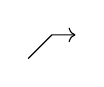
\begin{tikzpicture}[xscale=0.3, yscale=0.3, baseline=(O)]
		\coordinate (O) at (0, -0.8);
		\draw[->] (0,-1) -- (1, 0) -- (2, 0);
	\end{tikzpicture}$
	给出 $f_h$; 方块部分的构造用到了定义 \ref{def:multiplicative-family} 的条件 (S3) 对右乘性系的版本, 下半部交换则属显然.
	
	运用 $\prod_k$ 的正合性可知 $u$ 是拟同构; 这又反过来说明 $g$ 也能由图表的
	$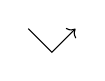
\begin{tikzpicture}[xscale=0.3, yscale=0.3, baseline=(O)]
		\coordinate (O) at (0, -0.8);
		\draw[->] (0,0) -- (1, -1) -- (2, 0);
	\end{tikzpicture}$
	部分确定. 然而 $Y \xrightarrow{c_k} M_k \xleftarrow{t_k} X_k$ 给出 $f_k$. 对照此前对 $f$ 的构造, 可见 $f = g$. 证毕.
\end{proof}

\begin{remark}
	若将积 (或余积) 的下标集换成任意小集 $I$, 仍有相应的陈述.
\end{remark}

命 $\mathcal{D}$ 为 $\cate{Ab}$-范畴. 考虑 \eqref{eqn:InvSys} 定义的范畴 $\cate{InvSys}(\mathcal{D}) := \mathcal{D}^{\Z_{\geq 0}^{\opp}}$, 其对象即资料 $X = (X_k, f_k)_{k \geq 0}$, 其中 $X_k \in \Obj(\mathcal{D})$ 而 $f_k \in \Hom_{\mathcal{D}}(X_{k+1}, X_k)$. 若 $\mathcal{D}$ 有可数积, 按定义 \ref{def:Delta-diff} 的方式定义典范态射
\[ \Delta_X := T_X - \identity: \prod_k X_k \to \prod_k X_k. \]
\index[sym1]{InvSys}
\index[sym1]{DirSys@$\cate{DirSys}$}

对偶地, 范畴 $\cate{DirSys}(\mathcal{D}) := \mathcal{D}^{\Z_{\geq 0}}$ 的对象即资料\footnote{又称为 $\mathcal{D}$ 中的正向系.} $X = (X_k, g_k)_{k \geq 0}$, 其中 $X_k \in \Obj(\mathcal{D})$ 而 $g_k \in \Hom_{\mathcal{D}}(X_k, X_{k+1})$. 以同样手法定义 $\nabla_X := T_X - \identity : \bigoplus_k X_k \to \bigoplus_k X_k$, 前提是 $\mathcal{D}$ 有可数余积; $T_X$ 仍是类似的平移态射.

假使 $\Ker(\Delta_X)$ 或 $\Coker(\nabla_X)$ 存在, 则有典范同构
\begin{align*}
	X \in \Obj\left( \cate{InvSys}(\mathcal{D}) \right) & \implies \varprojlim_k X_k \simeq \Ker(\Delta_X), \\
	X \in \Obj\left( \cate{DirSys}(\mathcal{D}) \right) & \implies \varinjlim_k X_k \simeq \Coker(\nabla_X).
\end{align*}
朴素的愿望是施此于 $\mathcal{D} = \cate{D}(\mathcal{A})$. 导出范畴鲜少是 Abel 范畴. 尽管如此, 注记 \ref{rem:homotopy-kernel-cokernel} 说明映射锥可充当核与余核的某种同伦版本; 三角范畴中粗略对应的构造是好三角.

\begin{definition}[M.\ Bökstedt, A.\ Neeman {\cite{BN93}}]\label{def:holim}
	\index{tonglunjixian@同伦极限, 同伦余极限 (homotopy limit, homotopy colimit)}
	\index[sym1]{holim@$\holim$, $\hocolim$}
	设 $\mathcal{D}$ 是三角范畴.
	\begin{itemize}
		\item 若 $\mathcal{D}$ 有可数积, 则 $\cate{InvSys}(\mathcal{D})$ 的对象 $X$ 的\emph{同伦极限} (或称同伦 $\varprojlim$) 意谓 $\mathcal{D}$ 的好三角
		\[ \holim(X) \to \prod_k X_k \xrightarrow{\Delta_X} \prod_k X_k \xrightarrow{+1} . \]
		\item 若 $\mathcal{D}$ 有可数余积, 则 $\cate{DirSys}(\mathcal{D})$ 的对象 $X$ 的\emph{同伦余极限} (或称同伦 $\varinjlim$) 意谓 $\mathcal{D}$ 的好三角
		\[ \bigoplus_k X_k \xrightarrow{\nabla_X} \bigoplus_k X_k \to \hocolim(X) \xrightarrow{+1} . \]
	\end{itemize}
\end{definition}

上述定义涉及的好三角彼此同构 (推论 \ref{prop:Cone-uniqueness}), 但同构非典范.

回到复形的讨论. 留意到 $\cate{InvSys}\left(\cate{C}(\mathcal{A})\right) = \cate{C}(\cate{InvSys}(\mathcal{A}))$, 两者的对象 $X$ 同为交换图表
\[\begin{tikzcd}
	& \vdots \arrow[d, "{f_1^n}"'] & \vdots \arrow[d, "{f_1^{n+1}}"] & \\
	\cdots \arrow[r] & X_1^n \arrow[r, "{d_{X_1}^n}"] \arrow[d, "{f_0^n}"'] & X_1^{n+1} \arrow[d, "{f_0^{n+1}}"] \arrow[r] & \cdots \\
	\cdots \arrow[r] & X_0^n \arrow[r, "{d_{X_0}^n}"] & X_0^{n+1} \arrow[r] & \cdots
\end{tikzcd} \quad \text{每行皆为复形}; \]
其间的态射同为双层交换图表. 依此遂可在 $\mathcal{D} := \cate{D}(\mathcal{A})$ 中比较 $\holim(X)$ 和 $\varprojlim$ 的右导出函子 $\mathrm{R}\lim(X)$, 前提是它们存在.

也留意到对 $\cate{C}(\cate{InvSys}(\mathcal{A}))$ 的对象 $X$ 取上同调 $\Hm^m$, 产物是 $\left(\Hm^m(X_k), \Hm^m(f_k)\right)_{k \geq 0}$. 所以 $X \to Y$ 是拟同构等价于每个 $X_k \to Y_k$ 都是 $\cate{C}(\mathcal{A})$ 中的拟同构.

\begin{theorem}\label{prop:Rlim-as-holim}
	设 $\mathcal{A}$ 为 Abel 范畴, 具有正合的可数积和足够的内射对象.
	\begin{enumerate}[(i)]
		\item 左正合函子 $\varprojlim: \cate{InvSys}(\mathcal{A}) \to \mathcal{A}$ 的右导出函子存在, 记为
		\[ \mathrm{R}\lim :  \cate{D}^+\left(\cate{InvSys}(\mathcal{A})\right) \to \cate{D}^+(\mathcal{A}) . \]
		\item 对 $\cate{C}^+(\cate{InvSys}(\mathcal{A}))$ 的任意对象 $X = (X_k, f_k)_{k \geq 0}$, 在 $\cate{D}(\mathcal{A})$ 中存在好三角
		\[ \mathrm{R}\lim(X) \to \prod_k X_k \xrightarrow{\Delta_X} \prod_k X_k \xrightarrow{+1} \]
		特别地, $\mathrm{R}\lim(X) \simeq \holim(X)$.
		\item 在定义--命题 \ref{def:dim-functor} 的意义下, $\mathrm{R}\lim$ 的维数 $\leq 1$.
	\end{enumerate}
\end{theorem}
\begin{proof}
	因为 $\cate{InvSys}(\mathcal{A})$ 有足够的内射对象, 故 (i) 成立. 更精确地说, 取引理 \ref{prop:lim1-prep} 的范畴 $\mathcal{R}$, 将 $\cate{InvSys}(\mathcal{A})$ 和 $\mathcal{R}$ 代入定理 \ref{prop:resolution-existence}, 可知对 $\cate{C}^+(\cate{InvSys}(\mathcal{A}))$ 的任意对象 $X = (X_k, f_k)_{k \geq 0}$, 存在拟同构 $X \to Y$ 使得 $Y \in \Obj\left( \cate{C}^+(\mathcal{R}) \right)$. 于是 $\mathrm{R}\lim(X) = \varprojlim Y$. 而 $\mathcal{R}$ 的定义又确保 $\Delta_Y$ 逐次满, 故有 $\cate{C}^+(\mathcal{A})$ 的短正合列
	\[ 0 \to \varprojlim Y \to \prod_{k \geq 0} Y_k \xrightarrow{\Delta_Y} \prod_{k \geq 0} Y_k \to 0. \]
	其次, $X_k \to Y_k$ 对每个 $k$ 皆是拟同构, 故 $\prod_{k \geq 0} X_k \to \prod_{k \geq 0} Y_k$ 也是拟同构. 这便给出 (ii) 断言的好三角
	\[ \mathrm{R}\lim(X) \to \prod_{k \geq 0} X_k \xrightarrow{\Delta_X} \prod_{k \geq 0} X_k \xrightarrow{+1} . \]

	至于 (iii), 注意到当 $X \in \Obj(\cate{InvSys}(\mathcal{A}))$ 时 $\Delta_X$ 简化为 $\cate{InvSys}(\mathcal{A})$ 的态射, 而 $\holim(X) \simeq \Cone(\Delta_X)[-1]$ 是 $\cate{D}^{[0,1]}(\mathcal{A})$ 的对象; 当然这也是定理 \ref{prop:lim1} 的复述. 
\end{proof}

对于 $\varinjlim: \cate{DirSys}(\mathcal{A}) \to \mathcal{A}$, 定理 \ref{prop:Rlim-as-holim} 有对偶版本, 不再赘述.

例 \ref{eg:Rlim-unbounded} 将说明如何对无界导出范畴得到 $\mathrm{R}\lim$, 使得定理 \ref{prop:Rlim-as-holim} (ii) 依然适用.

\section{无界导出函子}\label{sec:unbounded-derived}
\index{daochuhanzi!无界 (unbounded)}
考虑 Abel 范畴之间的加性函子 $F: \mathcal{A} \to \mathcal{A}'$. 本节回到定义 \ref{def:derived-functor}, 着重探讨无界导出范畴版本的导出函子
\[ \mathrm{R}F, \; \mathrm{L}F: \cate{D}(\mathcal{A}) \to \cate{D}(\mathcal{A}'). \]

为了确保 $\mathrm{R}F$ 或 $\mathrm{L}F$ 存在并进行操作, 需要定义 \ref{def:K-resolutions} 的 K-内射复形或 K-投射复形, 以及相应的解消等概念.

\begin{lemma}\label{prop:K-injective-zero}
	设 $\mathcal{A}$ 为 Abel 范畴. 设 $Z \in \Obj(\cate{K}(\mathcal{A}))$ 既是 K-内射 (或 K-投射) 又是零调的, 则 $Z = 0$.
\end{lemma}
\begin{proof}
	引理 \ref{prop:K-injective-criterion} 蕴涵 $\Hom_{\cate{K}(\mathcal{A})}(Z, Z) = 0$.
\end{proof}

兹陈述一则一般结果. 选定三角范畴 $\mathcal{D}_1, \mathcal{D}_2, \mathcal{D}'$ 及其饱和子三角范畴 $\mathcal{N}_1, \mathcal{N}_2, \mathcal{N}'$.

\begin{lemma}\label{prop:K-cats}
	给定三角双函子 $G: \mathcal{D}_1 \times \mathcal{D}_2 \to \mathcal{D}'$, 定义 $\mathcal{D}_2$ 的全子范畴 $\mathcal{K}_2^G$ 使得
	\[ \Obj(\mathcal{K}_2^G) = \left\{ X_2 \in \Obj(\mathcal{D}_2) : X_1 \in \Obj(\mathcal{N}_1) \implies G(X_1, X_2) \in \Obj(\mathcal{N}') \right\}, \]
	则 $\mathcal{K}_2^G$ 是饱和子三角范畴. 如将变元位置调换, 相应的叙述对 $\mathcal{K}_1^G \subset \mathcal{D}_1$ 依然成立.
\end{lemma}
\begin{proof}
	由 $G(X_1, X_2[1]) \simeq G(X_1, X_2)[1]$ 可知 $\mathcal{K}_2^G$ 对平移封闭. 同理, 设有好三角 $I \to J \to K \xrightarrow{+1}$, 其中 $I, K \in \Obj(\mathcal{K}_2^G)$, 则从好三角
	\[ G(X_1, I) \to G(X_1, J) \to G(X_1, K) \xrightarrow{+1} \]
	容易看出 $X_1 \in \Obj(\mathcal{N}_1) \implies G(X_1, J) \in \Obj(\mathcal{N}')$. 饱和性质是自明的.
\end{proof}

此结果可以应用于 $\Hom: \mathcal{A}^{\opp} \times \mathcal{A} \to \cate{Ab}$ 以及相应的三角双函子 $\cate{K}_{\Pi}\Hom$. 例 \ref{eg:Hom-bicplx} 已经说明后者本质上即是 $\Hom$ 复形:
\begin{equation}\label{eqn:CPiHom}\begin{gathered}
	(\cate{C}_{\Pi} \Hom)(\sigma^{-1} X_1, X_2) \simeq \Hom^\bullet\left( X_1, X_2 \right), \\
	(\cate{K}_\Pi \Hom)(\sigma^{-1} X_1, X_2) \simeq \Hom^\bullet\left( X_1, X_2 \right)\; \text{在 $\cate{K}(\cate{Ab})$ 中的像},
\end{gathered}\end{equation}
其中 $\sigma: \cate{C}(\mathcal{A}^{\opp}) \rightiso \cate{C}(\mathcal{A})^{\opp}$ 和 $\cate{K}(\mathcal{A}^{\opp}) \rightiso \cate{K}(\mathcal{A})^{\opp}$ 如定义--命题 \ref{def:sigma} 和命题 \ref{prop:sigma-homotopy}. 稍后将需要它的导出范畴版本.

\begin{proposition}\label{prop:K-injective-F-injective}
	全体 K-内射复形 (或 K-投射复形) 构成 $\cate{K}(\mathcal{A})$ 的饱和子三角范畴 $\mathcal{I}$ (或 $\mathcal{P}$). 若 $\mathcal{A}$ 有足够的 K-内射 (或 K-投射) 复形, 则 $\mathcal{I}$ (或 $\mathcal{P}$) 对任意加性函子 $F: \mathcal{A} \to \mathcal{A}'$ 都是 $F$-内射的 (或 $F$-投射的).
\end{proposition}
\begin{proof}
	仅论 K-内射情形. 前半部是配合 K-内射复形的定义 \ref{def:K-resolutions} 和 \eqref{eqn:CPiHom}, 将引理 \ref{prop:K-cats} 施于 $G = \cate{K}_{\Pi}\Hom$ 的结果: 该处的 $\mathcal{K}_2^G$ 正是此处的 $\mathcal{I}$.
	
	设 $\mathcal{A}$ 有足够的 K-内射复形. 若 $I$ 是零调 K-内射复形, 则引理 \ref{prop:K-injective-zero} 蕴涵 $I = 0$, 故 $(\cate{K}F)I$ 当然零调. 因此定义 \ref{def:F-injective} 对 $F$-内射子三角范畴的全部条件成立.
\end{proof}

命 $Q: \cate{K}(\mathcal{A}) \to \cate{D}(\mathcal{A})$ 和 $Q': \cate{K}(\mathcal{A}') \to \cate{D}(\mathcal{A}')$ 为局部化函子.

\begin{corollary}
	若 $\mathcal{A}$ 有足够的 K-内射复形, 则 $F$ 有右导出函子 $\mathrm{R}F: \cate{D}(\mathcal{A}) \to \cate{D}(\mathcal{A}')$, 使得当 $X$ 为 K-内射复形时 $\mathrm{R}F(QX) \simeq Q' \cate{K}F(X)$.
	
	对偶地, 若 $\mathcal{A}$ 有足够的 K-投射复形, 则 $F$ 有左导出函子 $\mathrm{L}F: \cate{D}(\mathcal{A}) \to \cate{D}(\mathcal{A}')$, 使得当 $X$ 为 K-投射复形时 $\mathrm{L}F(QX) \simeq Q' \cate{K}F(X)$.
\end{corollary}
\begin{proof}
	将命题 \ref{prop:K-injective-F-injective} 的结论代入命题 \ref{prop:localization-injective} 的一般框架.
\end{proof}

现在选定 Abel 范畴 $\mathcal{A}_1$, $\mathcal{A}_2$, $\mathcal{B}$. 对加性双函子 $F: \mathcal{A}_1 \times \mathcal{A}_2 \to \mathcal{B}$ 考虑定义 \ref{def:derived-bifunctor} 的导出双函子 $\mathrm{R}F$ (或 $\mathrm{L}F$) 的无界版本; 以下皆假设 $\mathcal{B}$ 有可数积 (或可数余积).

具体地说, 我们希望以上述子范畴 $\mathcal{I}_1$, $\mathcal{I}_2$ (或 $\mathcal{P}_1$, $\mathcal{P}_2$) 确定 $\mathrm{R}F$ (或 $\mathrm{L}F$).

\begin{lemma}\label{prop:bifunctor-via-K-injective-prep}
	取 $\cate{K}(\mathcal{A}_i)$ 的子三角范畴 $\mathcal{I}_i$ (或 $\mathcal{P}_i$) 如命题 \ref{prop:K-injective-F-injective}, 其中 $i=1, 2$.
	\begin{compactitem}
		\item 若 $\mathcal{A}_1$ 和 $\mathcal{A}_2$ 有足够的 K-内射复形, 则 $\mathcal{I}_1 \times \mathcal{I}_2$ 是 $F$-内射的.
		\item 若 $\mathcal{A}_1$ 和 $\mathcal{A}_2$ 有足够的 K-投射复形, 则 $\mathcal{P}_1 \times \mathcal{P}_2$ 是 $F$-投射的.
	\end{compactitem}
\end{lemma}
\begin{proof}
	仅论 K-内射情形. 关键在于说明若 $X_1 \in \Obj(\mathcal{I}_1)$, 则 $(\cate{K}_{\Pi} F)(X_1, \cdot)$ 映 $\mathcal{I}_2$ 的所有零调对象 $Z$ 为 $\cate{K}(\mathcal{B})$ 的零调对象. 但引理 \ref{prop:K-injective-zero} 说明 $Z=0$, 而 $(\cate{K}_{\Pi} F)(X_1, \cdot)$ 是加性函子, 故这是当然的. 下标 $1, 2$ 调换后也有相应的结果.
\end{proof}

命 $Q: \cate{K}(\mathcal{B}) \to \cate{D}(\mathcal{B})$ 和 $Q_i: \cate{K}(\mathcal{A}_i) \to \cate{D}(\mathcal{A}_i)$ 为局部化函子 ($i=1,2$).

\begin{proposition}\label{prop:bifunctor-via-K-injective}
	给定 $F: \mathcal{A}_1 \times \mathcal{A}_2 \to \mathcal{B}$, 设 $\mathcal{A}_1$ 和 $\mathcal{A}_2$ 皆有足够的 K-内射 (或 K-投射) 复形, 则导出双函子 $\mathrm{R}F$ (或 $\mathrm{L}F$) 存在. 若 $X_i \in \Obj(\cate{K}(\mathcal{A}))$ 对 $i=1, 2$ 都是 K-内射的 (或 K-投射的), 则有典范同构
	\[ \mathrm{R}F(Q_1 X_1, Q_2 X_2) \simeq Q (\cate{K}_{\Pi} F)(X_1, X_2) \quad \text{(或 $\mathrm{L}F(Q_1 X_1, Q_2 X_2) \simeq Q (\cate{K}_{\oplus} F)(X_1, X_2)$) }. \]
\end{proposition}
\begin{proof}
	直接将引理 \ref{prop:bifunctor-via-K-injective-prep} 的结果代入命题 \ref{prop:localization-injective-bifunctor}.
\end{proof}

对于具体给定的双函子 $F$, 经常可以取到比 K-内射 (或 K-投射) 复形更大的 $F$-内射 (或 $F$-投射) 子三角范畴. 以下着重讨论的 $\RHom$ 即是一例.

\begin{theorem}[无界 $\RHom$]\label{prop:unbounded-RHom}
	\index{RHom hanzi}
	\index[sym1]{RHom}
	设 Abel 范畴 $\mathcal{A}$ 有足够的 K-内射复形, 或足够的 K-投射复形. 将局部化函子统一记为 $Q$ 以简化符号.
	\begin{enumerate}[(i)]
		\item 双函子 $\Hom = \Hom_{\mathcal{A}}: \mathcal{A}^{\opp} \times \mathcal{A} \to \cate{Ab}$ 有右导出函子 $\cate{D}(\mathcal{A}^{\opp}) \times \cate{D}(\mathcal{A}) \to \cate{D}(\cate{Ab})$, 它也可以通过命题 \ref{prop:derived-cat-op} 的等价 $\sigma$ 写作
		\[ \RHom: \cate{D}(\mathcal{A})^{\opp} \times \cate{D}(\mathcal{A}) \to \cate{D}(\cate{Ab}). \]
		事实上, 若 $\mathcal{A}$ 有足够的 K-内射 (或 K-投射) 复形, 则 $\cate{K}(\mathcal{A})^{\opp} \times \mathcal{I}$ (或 $\mathcal{P}^{\opp} \times \cate{K}(\mathcal{A})$) 是 $\Hom$-内射的.
		\item 设 $\mathcal{A}$ 有足够的 K-内射复形, $X_2 \to I_2$ 是 K-内射解消, 则它诱导
		\[ \RHom(Q X_1, Q X_2) \rightiso Q \Hom^\bullet(X_1, I_2). \]
		作为特例, $\RHom(Q X_1, \cdot) \simeq \mathrm{R}\left( \Hom(X_1, \cdot) \right)$.
		\item 设 $\mathcal{A}$ 有足够的 K-投射复形, $P_1 \to X_1$ 是 K-投射解消, 则它诱导
		\[ \RHom(Q X_1, Q X_2) \rightiso Q \Hom^\bullet(P_1, X_2). \]
		作为特例, $\RHom(\cdot, Q X_2) \simeq \mathrm{R}\left(\Hom(\cdot, X_2)\right)$.
		\item 存在典范同构 $\Hm^n \RHom(X, Y) \simeq \Hom_{\cate{D}(\mathcal{A})}(X, Y[n]) =: \Ext^n(X, Y)$ (定义 \ref{def:Ext-general}).
	\end{enumerate}
\end{theorem}
\begin{proof}
	和定理 \ref{prop:RHom-bounded} 几乎平行. 以 $\mathcal{A}$ 有足够的 K-内射复形的情形为例, 关键在于说明 $\cate{K}(\mathcal{A})^{\opp} \times \mathcal{I}$ 是 $\Hom$-内射的.
	\begin{itemize}
		\item 固定复形 $X_1$, 函子 $(\cate{K}_\Pi \Hom)(X_1, \cdot)$ 映一切零调 K-内射复形 $X_2$ 为零调复形, 这是因为 $X_2$ 在 $\cate{K}(\mathcal{A})$ 中为 $0$ (引理 \ref{prop:K-injective-zero}).
		\item 固定 K-内射复形 $X_2$, 设复形 $X_1$ 零调, 则 K-内射复形的定义导致 $\Hom^\bullet\left( X_1, X_2 \right)$ 零调, 代入 \eqref{eqn:CPiHom} 可见 $(\cate{K}_\Pi \Hom)(X_1, X_2)$ 也零调.
	\end{itemize}
	这便验证了 $\Hom$-内射所需的零调条件, 而解消条件是平凡的.
\end{proof}

\begin{theorem}\label{prop:RHom-adjoint}
	考虑 Abel 范畴之间的一对伴随加性函子
	$\begin{tikzcd}
		F: \mathcal{A} \arrow[r, shift left] & \mathcal{A}' \arrow[l, shift left] : G
	\end{tikzcd}$.
	设 $\mathcal{A}$ 有足够的 K-投射复形, $\mathcal{A}'$ 有足够的 K-内射复形. 此时存在 $\cate{D}(\cate{Ab})$ 中的典范同构
	\[ \RHom_{\mathcal{A'}}\left(\mathrm{L}F(X), Y\right) \simeq \RHom_{\mathcal{A}}\left(X, \mathrm{R}G(Y) \right), \]
	其中 $X \in \Obj\left(\cate{D}(\mathcal{A})\right)$, $Y \in \Obj\left(\cate{D}(\mathcal{A}')\right)$.
\end{theorem}
\begin{proof}
	论证和定理 \ref{prop:RHom-adjoint-bounded} 相同. 唯一差别在于以 K-内射 (或 K-投射) 解消代替内射 (或投射) 解消, 并且以定理 \ref{prop:K-resolution-homotopy} 代替定理 \ref{prop:resolution-homotopy} 来探讨解消的唯一性.
\end{proof}

\begin{remark}
	对定理 \ref{prop:RHom-adjoint} 两边同取 $\Hm^0$, 即有伴随关系
	\[ \Hom_{\cate{D}(\mathcal{A'})}\left(\mathrm{L}F(X), Y\right) \simeq \Hom_{\cate{D}(\mathcal{A})}\left(X, \mathrm{R}G(Y) \right). \]

	由于通过解消得到的导出函子总是定义 \ref{def:absolute-Kan} 的绝对 Kan 延拓 (命题 \ref{prop:localization-functor-abs}), 定理 \ref{prop:Quillen-adjunction-gen} 也断言 $(\mathrm{L}F, \mathrm{R}G)$ 是伴随对. 两者给出相同的伴随同构. 何以故? 问题化约到 $X$ 是 K-投射复形而 $Y$ 是 K-内射复形的情形, 此时定理 \ref{prop:RHom-adjoint} 的伴随同构通过 $\cate{K}(\cdot)$ 层次的单位 $\eta$ 和余单位 $\varepsilon$ 具体实现为
	\begin{align*}
		\Hom_{\cate{K}(\mathcal{A}')}\left( \cate{K}F(X), Y\right) \simeq \Hom_{\cate{K}(\mathcal{A})}\left( X, \cate{K}G(Y) \right).
	\end{align*}
	另一方面, 定理 \ref{prop:Quillen-adjunction-gen} 在导出范畴层次确定了 $\underline{\eta}$ 和 $\underline{\varepsilon}$, 该处给出的刻画足以说明它们和 $\eta$, $\varepsilon$ 相容. 细节请感兴趣的读者琢磨.
\end{remark}

最后, 得到无界导出函子的另一套充分条件是基于维数的有限性 (定义--命题 \ref{def:dim-functor}). 虽然其证明技术不超出本书范围, 为了避免岔题, 权且述而不证. 详见 {\cite[Tags 07K6, 07K7]{stacks}}. 我们的起点是定理 \ref{prop:derived-via-resolution} 对有界导出函子的构造.

\begin{proposition}\label{prop:unbounded-derived-fd}
	\index{weishu}
	取 $F: \mathcal{A} \to \mathcal{A}'$ 为 Abel 范畴之间的左正合 (或右正合) 函子. 假设
	\begin{compactitem}
		\item 相对于 $F$, 存在 $\mathcal{A}$ 的 I 型 (或 P 型) 加性全子范畴 $\mathcal{A}^\flat$, 如定义--命题 \ref{prop:F-injective-criterion};
		\item 相应的有界导出函子 ${}^+ \mathrm{R}F$ (或 ${}^- \mathrm{L}F$) 维数有限.
	\end{compactitem}
	此时 $\mathrm{R}F$ (或 $\cate{L}F$): $\cate{D}(\mathcal{A}) \to \cate{D}(\mathcal{A}')$ 存在; 事实上, $\cate{K}(\mathcal{A}^\flat)$ 构成 $\cate{K}(\mathcal{A})$ 的 $F$-内射 (或 $F$-投射) 子范畴.
\end{proposition}

\begin{example}\label{eg:Rlim-unbounded}
	设 $\mathcal{A}$ 具有正合的可数积和足够的内射对象. 取左正合函子 $F$ 为 $\varprojlim: \cate{InvSys}(\mathcal{A}) \to \mathcal{A}$. 定理 \ref{prop:Rlim-as-holim} (iii) 说明有界版本 $\mathrm{R}\lim$ 的维数 $\leq 1$, 子范畴 $\mathcal{R} \subset \cate{InvSys}(\mathcal{A})$ 对之是 I 型的. 前述结果因而给出无界导出函子
	\[ \mathrm{R}\lim: \cate{D}(\cate{InvSys}(\mathcal{A})) \to \cate{D}(\mathcal{A}). \]
	
	一如定理 \ref{prop:Rlim-as-holim} (ii) 的情形, 对 $\cate{C}(\cate{InvSys}(\mathcal{A}))$ 的所有对象 $X$ 皆有 $\cate{D}(\mathcal{A})$ 的好三角
	\[ \mathrm{R}\lim(X) \to \prod_k X_k \xrightarrow{\Delta_X} \prod_k X_k \xrightarrow{+1} . \]
	特别地, $\mathrm{R}\lim(X) \simeq \holim(X)$. 基于命题 \ref{prop:unbounded-derived-fd} 的结论, 原证明可以照搬: 将一切 $\cate{C}^+(\cdots)$ 直接改为 $\cate{C}(\cdots)$ 便是.
\end{example}

\section{实例: K-平坦复形和 \texorpdfstring{$\otimesL$}{otimesL}}\label{sec:otimesL}
本节选定交换环 $\Bbbk$.

\begin{convention}\label{con:bimodule-algebra}
	设 $R$, $S$ 为 $\Bbbk$-代数, 按本书惯例, $(R,S)$-双模 $M$ 默认满足 $tm = mt$, 其中 $t \in \Bbbk$ 而 $m \in M$. 换言之 $(R,S)\dcate{Mod} \simeq (R \dotimes{\Bbbk} S^{\opp})\dcate{Mod}$. 当 $\Bbbk = \Z$ 时, 此条件是多余的.
	
	今后将忘却函子 $(R,S)\dcate{Mod} \to R\dcate{Mod}$ (或 $(R,S)\dcate{Mod} \to \cated{Mod}S$) 记为 $M \mapsto {}_R M$ (或 $M \mapsto M_S$); 同样记法适用于复形. 忘却函子是正合的, 它们在导出范畴之间诱导的三角函子也按相同方式标记.
\end{convention}

一则平凡的观察: 对于任何由 $(R, S)$-双模构成的复形 $M$, 我们有
\[ M_S \;\text{零调} \iff M \;\text{零调} \iff {}_R M \;\text{零调}. \]

今后设 $R$, $A$, $B$ 为 $\Bbbk$-代数. 我们的出发点是张量积给出的双函子
\[ \otimes_R: (A, R)\dcate{Mod} \times (R, B)\dcate{Mod} \to (A, B)\dcate{Mod}, \]
它对每个变元都右正合. 最单纯的是 $A = \Bbbk = B$ 的情形, 对应的双函子化为 $\otimes_R: \cated{Mod}R \times R\dcate{Mod} \to \cate{\Bbbk}$.

简单起见, 对于 $(A,R)$-双模构成的复形 $X$ 和 $(R,B)$-双模构成的复形 $Y$, 今后将逐项作张量积得到的双复形记为 $X^\bullet \dotimes{R} Y^\bullet$, 而将其全复形记为
\[ X \dotimes{R} Y := \tot_{\oplus} \left( X^\bullet \dotimes{R} Y^\bullet \right). \]

双模范畴有足够的 K-投射复形 (应用例 \ref{eg:Mod-K-injectives}), 故命题 \ref{prop:bifunctor-via-K-injective} 确保无界左导出双函子存在.

\begin{definition}\label{def:otimesL}
	\index{daochuzhangliangji@导出张量积 (derived tensor product)}
	\index[sym1]{XotimesLY@$X \otimesL[R] Y$}
	记 $\otimes_R$ 的左导出函子 $\mathrm{L}\left( \cdot \dotimes{R} \cdot \right)$ 为
	\[ \otimesL[R] : \cate{D}((A, R)\dcate{Mod}) \times \cate{D}((R, B)\dcate{Mod}) \to \cate{D}((A, B)\dcate{Mod}). \]
	不致混淆时, 也将 $X \otimesL[R] Y$ 简记为 $X \otimesL Y$.
\end{definition}

上述抽象定义直截了当, 但仍须引入称为 K-平坦解消的一类拟同构来助推 $\otimes_R$ 的研究, 理由包括:
\begin{itemize}
	\item K-平坦解消的定义与张量积直接相关, 而且对于确立一些重要性质和实际计算更有意义, 这点在 \S\ref{sec:Ext-Tor} 已有体现;
	\item 在层论等几何场景中, 可能仅有 K-内射解消而无 K-投射解消, 此时 K-平坦解消是研究导出张量积的唯一手段.
\end{itemize}

\begin{definition}[N.\ Spaltenstein {\cite[Definition 5.1]{Spa88}}]
	\index{fuxing!K-平坦 (K-flat)}
	设 $X$ 为右 $R$-模构成的复形. 若对所有由左 $R$-模构成的复形 $Y$,
	\[ Y \;\text{零调} \implies X \dotimes{R} Y\;\text{零调}, \]
	则称 $X$ 是 \emph{K-平坦}的\footnote{更合理的名称兴许是同伦平坦复形.}; 此性质仅关乎 $X$ 在 $\cate{K}(\cated{Mod}R)$ 中的同构类. 类似手法可对左 $R$-模构成的复形定义何谓 K-平坦.
\end{definition}

对于上有界复形, K-平坦性可归结为模论中熟知的平坦性.

\begin{proposition}\label{prop:flat-K-flat}
	设 $X$ 为 $\cate{C}^-(\cated{Mod}R)$ 的对象, 而且每个 $X^n$ 皆平坦, 则 $X$ 是 K-平坦的. 对  $\cate{C}^-(R\dcate{Mod})$ 的对象亦同.
\end{proposition}
\begin{proof}
	设 $Y$ 为左 $R$-模构成的零调复形, 今将往证 $X \dotimes{R} Y$ 零调. 应用截断函子将 $Y$ 表为 $\varinjlim_m \tau^{\leq m} Y$. 逐次地看, $\varinjlim_m$ 既和张量积交换 \cite[命题 6.9.2]{Li1}, 又和 $\bigoplus$ 交换, 问题因此化到 $Y$ 上有界的情形. 于是 $X^\bullet \dotimes{R} Y^\bullet$ 落在定义 \ref{def:Cf-Supp} 的范畴 $\cate{C}^2_f(\Bbbk\dcate{Mod})$. 因为 $X^p \dotimes{R} Y^\bullet$ 对每个 $p$ 皆零调, 推论 \ref{prop:acyclic-assembly} 确保 $X \dotimes{R} Y$ 零调.
\end{proof}

有鉴于此, 倘若读者只关心上有界导出范畴, 则不妨将本节出现的所有 K-平坦复形都代换为由平坦模构成的上有界复形.

\begin{definition}
	\index{jiexiao!K-平坦 (K-flat)}
	\index{zugoude K-pingtan fuxing@足够的 K-平坦复形 (enough K-flats)}
	若 $P \to X$ 是 $\cate{C}((A,R)\dcate{Mod})$ 中的拟同构, 而且 $P_R$ 是 K-平坦的, 则称之为 $X$ 对 $R$ 的 \emph{K-平坦解消}. 如果所有 $X \in \cate{C}((A, R)\dcate{Mod})$ 都有对 $R$ 的 K-平坦解消, 则称 $(A, R)\dcate{Mod}$ 对 $R$ 有足够的 K-平坦复形.
	
	以类似手法定义 $X \in \Obj(\cate{C}((R, B)\dcate{Mod}))$ 对 $R$ 的 K-平坦解消.
\end{definition}

我们自然要问: 如何确保双模范畴对 $R$ 有足够的 K-平坦复形? K-平坦和 K-投射复形之间有何关系? 毫不意外, 桥梁来自 $\otimes$ 和 $\Hom$ 之间经典的伴随关系 \cite[定理 6.6.5]{Li1}.

为此, 首务是将伴随关系升级到复形层次. 若 $Y$ 为 $\cate{C}((R, B)\dcate{Mod})$ 的对象, $Z$ 为 $\cate{C}((A, B)\dcate{Mod})$ 的对象, 则 $\Hom$ 复形 $\Hom^\bullet(Y_B, Z_B)$ 可逐次地赋予 $(A, R)$-双模结构, 这给出 $\cate{C}((A, R)\dcate{Mod})$ 的对象.

\begin{proposition}[$\Hom$ 和 $\otimes$ 的伴随关系: 复形版本]\label{prop:tensor-Hom-cplx}
	设 $X$ 为 $\cate{C}((A, R)\dcate{Mod})$ 的对象, $Y$ 为 $\cate{C}((R, B)\dcate{Mod})$ 的对象, $Z$ 为 $\cate{C}((A, B)\dcate{Mod})$ 的对象. 存在 $\cate{C}(\Bbbk\dcate{Mod})$ 中的典范同构
	\begin{align*}
		\Hom^\bullet\left( X \dotimes{R} Y, \; Z \right) & \simeq \Hom^\bullet\left( X, \Hom^\bullet(Y_B, Z_B) \right) \\
		& \simeq \Hom^\bullet\left( Y, \Hom^\bullet({}_A X, {}_A Z) \right).
	\end{align*}

	作为推论, 取 $\Ker(d^0)$ 便有 $\Bbbk$-模的同构
	\begin{align*}
		\Hom_{\cate{C}((A, B)\dcate{Mod})}\left( X \dotimes{R} Y, \; Z \right) & \simeq \Hom_{\cate{C}((A, R)\dcate{Mod})}\left( X, \Hom^\bullet(Y_B, Z_B) \right) \\
		& \simeq \Hom_{\cate{C}((R, B)\dcate{Mod})}\left( Y, \Hom^\bullet({}_A X, {}_A Z) \right).
	\end{align*}
\end{proposition}
\begin{proof}
	处理第一个同构即可. 为简化计, 以下将 $Y_B$ 和 $Z_B$ 直接记为 $Y$ 和 $Z$, 同时省略 $\Hom$ 的下标. 选定 $n \in \Z$. 同构左侧的 $n$ 次项是
	\begin{multline}\label{eqn:tensor-Hom-cplx-aux}
		\prod_k \Hom\left( (X \dotimes{R} Y)^k, Z^{k+n}\right) \simeq \prod_k \prod_{p+q=k} \Hom\left(X^p \dotimes{R} Y^q, Z^{k+n}\right) \\
		= \prod_{p, q} \Hom\left( X^p \dotimes{R} Y^q, Z^{p+q+n} \right) \simeq \prod_p \prod_q \Hom\left( X^p, \Hom\left(Y^q, Z^{p+q+n}\right) \right) \\
		\simeq \prod_p \Hom\left( X^p, \Hom^{p+n}(Y, Z) \right),
	\end{multline}
	末项即同构右侧的 $n$ 次项. 具体地说, $(A, B)$-双模同态 $\varphi^{p, q}: X^p \dotimes{R} Y^q \to Z^{p+q+n}$ 在第二个 $\simeq$ 之下对应
	\[ \left[ x \mapsto [y \mapsto \varphi^{p,q}(x \otimes y)] \right] \; \in \Hom\left( X^p, \Hom\left(Y^q, Z^{p+q+n}\right) \right). \]
	后续工作只剩下验证 \eqref{eqn:tensor-Hom-cplx-aux} 确定复形的同构.
	
	给定左侧的 $n$ 次项元素, 表作 $(\varphi^{p,q})_{p, q \in \Z}$, 它对 $d_{\Hom^\bullet(X \otimes Y, Z)}$ 的像的 $(p, q)$ 分量映 $x \otimes y \in X^p \dotimes{R} Y^q$ 为
	\[ d_Z \varphi^{p,q}(x \otimes y) - (-1)^n \left( \varphi^{p+1, q}(d_X x \otimes y) + (-1)^p \varphi^{p, q+1}(x \otimes d_Y y) \right). \]
	
	对于右侧相应的 $n$ 次项元素, 它对 $d_{\Hom^\bullet(X, \Hom^\bullet(Y, Z))}$ 的像的 $p$ 分量映 $x \in X^p$ 为
	\[
		d_{\Hom^\bullet(Y, Z)}\left[ y \mapsto \varphi^{p,q}(x \otimes y) \right]_{q \in \Z} - (-1)^n \left[ y \mapsto \varphi^{p+1, q}(d_X x \otimes y) \right]_{q \in \Z};
	\]
	进一步展开 $d^{p+n}_{\Hom^\bullet(Y, Z)}$ 的定义可见对于选定的 $(p, q)$, 此即
	\[ y \mapsto d_Z \varphi^{p,q}(x \otimes y) - (-1)^{p+n} \varphi^{p, q+1}(x \otimes d_Y y) - (-1)^n \varphi^{p+1, q}(d_X x \otimes y). \]
	明所欲证.
\end{proof}

现在回到 K-投射复形和 K-平坦复形的联系.

\begin{lemma}\label{prop:K-projective-flat}
	设 $X$ 是 $(A, R)$-双模构成的 K-投射复形, 则当 $A$ 是平坦 $\Bbbk$-模时, $X_R$ 是 K-平坦的.
	
	设 $Y$ 是 $(R, B)$-双模构成的 K-投射复形, 则当 $B$ 是平坦 $\Bbbk$-模时, ${}_R Y$ 是 K-平坦的.
\end{lemma}
\begin{proof}
	处理第一则断言即可. 取左 $R$-模构成的零调复形 $Y$. 对于任意左 $A$-模 (亦即 $(A, \Bbbk)$-双模) $I$, 视同集中在零次项的复形, 命题 \ref{prop:tensor-Hom-cplx} (代入 $B = \Bbbk$) 给出
	\[ \Hom^\bullet\left(X \dotimes{R} Y, \; I\right) \simeq \Hom^\bullet\left(X, \Hom^\bullet(Y_{\Bbbk}, I_{\Bbbk}) \right). \]
	
	设 $I$ 为内射左 $A$-模, 则 $I_{\Bbbk}$ 是内射 $\Bbbk$-模, 原因是忘却函子 $A\dcate{Mod} \to \Bbbk\dcate{Mod}$ 有正合左伴随 $A \dotimes{\Bbbk} (\cdot)$; 见命题 \ref{prop:adjoint-injective-projective} 和 \cite[推论 6.6.8]{Li1}. 于是 $\Bbbk$-模的复形 $\Hom^\bullet(Y_{\Bbbk}, I_{\Bbbk})$ 零调, 它作为 $(A, R)$-双模的复形依然零调, 从而 $X$ 的 K-投射性质蕴涵 $\Hom^\bullet(X \dotimes{R} Y, I)$ 零调.

	既然 $I$ 内射, 易见对所有 $n \in \Z$ 皆有
	\[ \Hom\left( \Hm^n\left( X \dotimes{R} Y \right), I\right) \simeq \Hm^{-n} \Hom^\bullet\left( X \dotimes{R} Y, \; I \right) = 0. \]
	
	又因为所有左 $A$-模都能嵌入内射模, $X \dotimes{R} Y$ 必零调. 证毕.
\end{proof}

倘若读者只关心交换环上的张量积, 亦即 $A, R, B$ 全部等于 $\Bbbk$ 的特例, 或者只关心 $\Bbbk$ 为域的情形, 则以上关于 $A$ 或 $B$ 的平坦条件平凡地成立.

\begin{corollary}\label{prop:enough-K-flat}
	若 $A$ (或 $B$) 是平坦 $\Bbbk$-模, 则 $(A,R)\dcate{Mod}$ (或 $(R,B)\dcate{Mod}$) 对 $R$ 有足够的 K-平坦复形.
\end{corollary}

如果进一步取 $A = \Bbbk$ (或 $B = \Bbbk$), 则上述结果表明右 (或左) $R$-模构成的 K-投射复形对 $R$ 总是 K-平坦的, 而 $\cated{Mod}R$ (或 $R\dcate{Mod}$) 有足够的 K-平坦复形.

现在说明如何以 K-平坦解消确定 $\otimes_R$ 的导出函子. 为简化计, 今后各种局部化函子 $Q$ 省略不标.

\begin{proposition}\label{prop:K-flat}
	定义 $\cate{K}((A, R)\dcate{Mod})$ 的全子范畴 $\mathcal{F}_{A, R}$, 使得
	\[ \Obj(\mathcal{F}_{A,R}) = \{ X: X_R \;\text{是 K-平坦的} \}; \]
	类似地定义 $\mathcal{F}_{R, B}$. 它们都是饱和三角子范畴. 以下探讨
	\[ \cate{K}((A,R)\dcate{Mod}) \times \cate{K}((R,B)\dcate{Mod}) \quad \text{的 $\otimes_R$-投射子范畴.} \]
	\begin{enumerate}[(i)]
		\item 设 $(A, R)\dcate{Mod}$ 对 $R$ 有足够的 K-平坦复形, 则 $\left(\mathcal{F}_{A, R}, \cate{K}((R,B)\dcate{Mod}) \right)$ 是 $\otimes_{R}$-投射子范畴. 作为推论, 设 $Y$ 是由 $(R,B)$-双模构成的复形, 则 $\cdot \otimesL[R] Y$ 是 $\cdot \dotimes{R} Y$ 的左导出函子, 可由 K-平坦解消计算.
		
		\item 设 $(R, B)\dcate{Mod}$ 对 $R$ 有足够的 K-平坦复形, 则 $(\cate{K}((A,R)\dcate{Mod}), \mathcal{F}_{R,B})$ 是 $\otimes_{R}$-投射子范畴. 作为推论, 设 $X$ 是由 $(A,R)$-双模构成的复形, 则 $X \otimesL[R] \cdot$ 是 $X \dotimes{R} \cdot$ 的左导出函子, 可由 K-平坦解消计算.
	\end{enumerate}
\end{proposition}
\begin{proof}
	引理 \ref{prop:K-cats} 说明 $\mathcal{F}_{A, R}$ 和 $\mathcal{F}_{R, B}$ 都是饱和子三角范畴. 对于后续部分, 讨论 (i) 即可. 回顾 \S\ref{sec:derived-functors} 相关定义, 可知关键是建立以下性质:
	\begin{itemize}
		\item 选定 $\mathcal{F}_{A,R}$ 中的复形 $X$, 若 $Y$ 是零调复形, 则 $X \dotimes{R} Y$ 零调;
		\item 选定 $Y$, 若 $X$ 是 $\mathcal{F}_{A, R}$ 中的零调复形, 则 $X \dotimes{R} Y$ 零调.
	\end{itemize}

	第一条性质由 K-平坦的定义自动保证. 现在考虑第二条. 由于 $X \dotimes{R} Y$ 只用到 $R$ 对 $Y$ 的左乘结构, 不妨设 $B = \Bbbk$. 此时推论 \ref{prop:enough-K-flat} 确保有 $\cate{C}(R\dcate{Mod})$ 中的 K-平坦解消 $Q \to Y$. 由此得到
	\begin{gather*}
		\cate{K}(R\dcate{Mod})\;\text{的好三角} \quad Q \to Y \to N \xrightarrow{+1}, \quad N: \text{零调复形}, \\
		 \cate{K}(A\dcate{Mod})\;\text{的好三角} \quad X \dotimes{R} Q \to X \dotimes{R} Y \to X \dotimes{R} N \xrightarrow{+1}.
	\end{gather*}
	既然 $X$ 零调而 $Q$ 是 K-平坦的, $X \dotimes{R} Q$ 零调. 又因为 $N$ 零调而 $X$ 对 $R$ 是 K-平坦的, $X \dotimes{R} N$ 零调. 综上可见 $X \dotimes{R} Y$ 亦零调.
	
	最后, 关于 $\otimesL[R]$ 的断言无非是命题 \ref{prop:localization-injective-bifunctor} (ii) 的直接应用.
\end{proof}

\begin{example}[环变换与 $\otimesL$]\label{eg:change-of-rings}
	\index{huanbianhuan@环变换 (change of rings)}
	\index[sym1]{PRS@${}_{R \to S} P$, $\mathrm{L} {}_{R \to S} P$, $P_{R \to S}$, $\mathrm{L} P_{R \to S}$}
	给定 $\Bbbk$-代数的同态 $R \to S$, 借此将 $S$ 视为 $(S, R)$-双模. 循 \cite[推论 6.6.8]{Li1} 的路线, 考虑右正合加性函子
	\begin{equation*}
		{}_{R \to S} P := S \dotimes{R} (\cdot): R\dcate{Mod} \to S\dcate{Mod} .
	\end{equation*}
	它有左导出函子 $\mathrm{L}{}_{R \to S} P$, 在推论 \ref{prop:enough-K-flat} 和命题 \ref{prop:K-flat} (ii) 中代入 $A = S$ 和 $B = \Bbbk$, 可见平坦性在此不成问题, 而
	\[ \mathrm{L}{}_{R \to S} P \simeq S \otimesL[R] (\cdot) . \]
	
	环变换还具有传递性: 给定同态 $R \to S \to T$, 则有典范同构
	\[ \mathrm{L} {}_{S \to T} P \circ \mathrm{L} {}_{R \to S} P \rightiso \mathrm{L} {}_{R \to T} P. \]
	诚然, 所示态射来自关于复合函子求导的定理 \ref{prop:localization-triangulated-composite}; 而因为
	\[ X \dotimes{S} (S \dotimes{R} Y) \simeq X_R \dotimes{R} Y, \quad X \in \Obj(\cate{C}(\cated{Mod}S)), \; Y \in \Obj(\cate{C}(R\dcate{Mod})), \]
	故 ${}_{R \to S} P$ 保持 K-平坦复形, 这就确保典范态射为同构.
	
	根据完全类似的手法, 可以定义 $P_{R \to S} = (\cdot) \dotimes{R} S: \cated{Mod}R \to \cated{Mod}S$ 的左导出函子 $\mathrm{L}P_{R \to S}$, 它由 $(\cdot) \otimesL[R] S$ 给出.
\end{example}

\begin{proposition}\label{prop:otimesL-enrichment}
	若 $A$ 或 $B$ 作为 $\Bbbk$-模是平坦的, 则有典范的 $2$-胞腔图表
	\[\begin{tikzcd}
		\cate{D}((A, R)\dcate{Mod}) \times \cate{D}((R, B)\dcate{Mod}) \arrow[r, "{\otimesL[R]}"] \arrow[d, "\text{忘却}"'] & \cate{D}((A, B)\dcate{Mod}) \arrow[d, "\text{忘却}"] \\
		\cate{D}(\cated{Mod}R) \times \cate{D}(R\dcate{Mod}) \arrow[r, "{\otimesL[R]}"'] \arrow[Rightarrow, ru, "\sim", sloped] & \cate{D}(\cate{Ab}) .
	\end{tikzcd}\]
\end{proposition}
\begin{proof}
	这类性质大多借助解消来论证. 扼要地说, 设 $X$ 是 $(A,R)$-双模构成的复形, $Y$ 是 $(R,B)$-双模构成的复形. 根据命题 \ref{prop:K-flat}, 不妨设 $X_R$ (或 ${}_R Y$) 是 K-平坦的; 此时 $X \dotimes{R} Y$ 同时给出第一行和第二行的 $\otimesL[R]$, 由此得到同构 $\Rightarrow$, 暂且记为 $\alpha$.
	
	如欲抽象地刻画 $\alpha$, 则可采用以下观点. 向所考察的图表另外叠加一层, 简单记为
	\[\begin{tikzcd}[column sep=small]
		& \cate{K}(\cdots) \times \cate{K}(\cdots) \arrow[dd] \arrow[ld, "\text{忘却}"'] \arrow[rr, "\dotimes{R}"] & & \cate{K}(\cdots) \arrow[dd] \arrow[ld, "\text{忘却}"'] \\
		\cate{K}(\cdots) \times \cate{K}(\cdots) \arrow[rr, crossing over, "\dotimes{R}" near end] \arrow[dd] & & \cate{K}(\cate{Ab}) & \\
		& \cate{D}(\cdots) \times \cate{D}(\cdots) \arrow[rr] \arrow[ld] & & \cate{D}(\cdots) \arrow[ld] \\
		\cate{D}(\cdots) \times \cate{D}(\cdots) \arrow[rr] & & \cate{D}(\cate{Ab}) \arrow[leftarrow, uu, crossing over] &
	\end{tikzcd}\]
	其中垂直箭头都是局部化函子. 我们希望将底面填充为
	$\begin{tikzcd}[row sep=small, column sep=small]
		\bullet \arrow[r] \arrow[d] & \bullet \arrow[d] \\
		\bullet \arrow[r] \arrow[Rightarrow, ru] & \bullet
	\end{tikzcd}$.
	方块的其余各面都容易处理: 基于左导出双函子的定义, 前后两面有如是填充; 基于局部化的泛性质, 左右两面精确到同构是交换的; 回顾张量积定义可知顶面也交换. 按图索骥, 可得合成函子之间的态射
	\[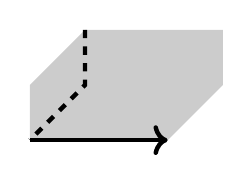
\begin{tikzpicture}[baseline, scale=0.7]
		\fill[gray!40] (0, 1) -- (-1, 0) -- (-1, -1) -- (1.5, -1) --(2.5, 0) -- (2.5, 1)  --cycle;
		\draw[ultra thick, dashed] (0,1) -- (0,0) -- (-1, -1);
		\draw[ultra thick, ->] (-1, -1) -- (1.5, -1);
	\end{tikzpicture} \;\Rightarrow \cdots \Rightarrow\; 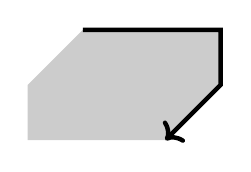
\begin{tikzpicture}[baseline, scale=0.7]
		\fill[gray!40] (-1, 1) -- (1.5, 1) -- (1.5, 0) -- (0.5, -1) -- (-2, -1) -- (-2, 0) --cycle;
		\draw[ultra thick, ->] (-1,1) -- (1.5 , 1) -- (1.5, 0)  -- (0.5, -1);
	\end{tikzpicture} \; =: \beth. \]
	
	回忆到 $\cate{D}(\cdots) \times \cate{D}(\cdots) \to \cate{D}(\cdots)$ 作为右 Kan 延拓是绝对的 (命题 \ref{prop:localization-functor-abs}), 故合成
	\begin{equation*}\begin{gathered}
		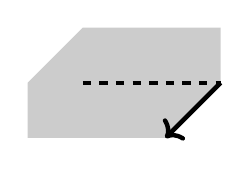
\begin{tikzpicture}[baseline=(O), scale=0.7]
			\fill[gray!40] (-1, 1) -- (1.5, 1) -- (1.5, 0) -- (0.5, -1) -- (-2, -1) -- (-2, 0) --cycle;
			\draw[ultra thick, dashed] (-1,0) -- (1.5, 0);
			\draw[ultra thick, ->] (1.5, 0)  -- (0.5, -1);
			\coordinate (O) at (0, 0);
		\end{tikzpicture}
		\quad \text{是 $\beth$ 沿} \quad
		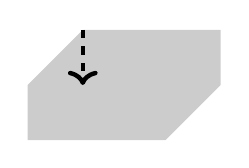
\begin{tikzpicture}[baseline=(O), scale=0.7]
			\fill[gray!40] (-1, 1) -- (1.5, 1) -- (1.5, 0) -- (0.5, -1) -- (-2, -1) -- (-2, 0) --cycle;
			\draw[ultra thick, dashed, ->] (-1, 1) -- (-1, 0);
			\coordinate (O) at (0, 0);
		\end{tikzpicture}
		\quad\text{的右 Kan 延拓.}
	\end{gathered}\end{equation*}
	应用映向 $\beth$ 的态射以及右 Kan 延拓的泛性质 (定义 \ref{def:Kan-extension}) 即得所求之 $\alpha$.
	
	一旦确认了 $\alpha$ 的存在性, 再按证明第一段的方式代入 K-平坦复形, 将一切函子提到上层计算, 即可证 $\alpha$ 为同构.
\end{proof}

今后经常省略这类基于泛性质的论证, 改以解消直接验证.

\begin{corollary}\label{prop:otimesL-Tor}
	\index[sym1]{Tor}
	定义 \ref{def:otimesL} 的函子 $\otimesL[R]$ 在 $A$ 或 $B$ 作为 $\Bbbk$-模平坦的条件下满足典范同构
	\[ \Hm^{-n}\left( X \otimesL[R] Y \right) \simeq \Tor^R_n(X, Y), \quad n \in \Z, \]
	其中 $X$ 是 $(A,R)$-双模, $Y$ 是 $(R,B)$-双模, $\Tor^R_n$ 如定义--命题 \ref{def:Tor-classical}.
\end{corollary}
\begin{proof}
	左式来自命题 \ref{prop:otimesL-enrichment} 的图表按
	\begin{tikzpicture}[xscale=0.3, yscale=0.3, baseline=(O)]
		\draw[->] (0,0) -- (1,0) -- (1, -1);
		\coordinate (O) at (0, -0.7);
	\end{tikzpicture}
	方向的合成, 右式来自按
	\begin{tikzpicture}[xscale=0.3, yscale=0.3, baseline=(O)]
		\draw[->] (0,0) -- (0, -1) -- (1, -1);
		\coordinate (O) at (0, -0.7);
	\end{tikzpicture}
	方向的合成.
\end{proof}

\begin{proposition}[结合约束]\label{prop:otimesL-associativity-constraint}
	\index{daochuzhangliangji!结合约束 (associativity constraint)}
	设 $A$, $B$, $R$, $S$ 为 $\Bbbk$-代数. 考虑以下两个函子
	\begin{gather*}
		\cate{D}((A,R)\dcate{Mod}) \times \cate{D}((R,S)\dcate{Mod}) \times \cate{D}((S,B)\dcate{Mod}) \to \cate{D}((A,B)\dcate{Mod}), \\
		(X, Y, Z) \mapsto (X \otimesL[R] Y) \otimesL[S] Z, \\
		(X, Y, Z) \mapsto X \otimesL[R] (Y \otimesL[S] Z).
	\end{gather*}
	若 $A$ 和 $B$ 作为 $\Bbbk$-模皆平坦, 则有典范同构
	\[ a(X,Y,Z): (X \otimesL[R] Y) \otimesL[S] Z \rightiso X \otimesL[R] (Y \otimesL[S] Z). \]
\end{proposition}
\begin{proof}
	固定 $Y$. 基于命题 \ref{prop:K-flat},	不妨设 $X_R$ 和 ${}_R Z$ 为 K-平坦的. 于是所有 $\otimesL[R]$ 都可以在复形的层次计算, 一切回归张量积的结合约束 \cite[命题 6.5.12]{Li1}.
\end{proof}

在平坦性的前提下, 三个以上的对象按种种次序取 $\otimesL$, 得到的结果依照结合约束两两同构; 这些同构也服从融贯性, 具体可以仿照幺半范畴的五角形公理来表述, 见 \cite[定义 3.1.1]{Li1}. 方法仍是取 K-平坦解消, 化到复形层次去验证. 本书省墨, 仅拈出交换环的特例.

\begin{example}[交换环的 $\otimesL$]\label{eg:commutative-otimesL}
	\index{daochuzhangliangji!交换约束 (commutativity constraint)}
	设 $R$ 为交换环. 在 $\otimesL := \otimesL[R]$ 的定义中将所有环取作 $R$, 特别地 $\Bbbk = R$, 如此则 $(R,R)\dcate{Mod} = R\dcate{Mod}$, 而之前关于平坦性的假设平凡地成立; 于是乎 $\Hm^{-n}(X \otimesL Y) \simeq \Tor^R_n(X,Y)$ 对所有 $R$-模 $X$, $Y$ 皆成立.
	
	这使得 $\cate{D}(R\dcate{Mod})$ 对 $\otimesL$ 成为 \cite[\S 3.1]{Li1} 介绍的幺半范畴, 其幺元由 $R$ 本身给出, 结合约束来自命题 \ref{prop:otimesL-associativity-constraint} 的 $a = (a(X,Y,Z))_{X,Y,Z}$. 留意到 $R$ 是平坦 $R$-模, 因而是 K-平坦的 (命题 \ref{prop:flat-K-flat}), 于是 $R \otimesL (\cdot)$ 和 $(\cdot) \otimesL R$ 皆可在复形层次计算, 由此易证幺半范畴的所有公理. 进一步, $\cate{D}(R\dcate{Mod})$ 还是 \cite[定义 3.3.1]{Li1} 的对称幺半范畴. 对应的辫结构 (或称交换约束) $c(X,Y): X \otimesL Y \rightiso Y \otimesL X$ 来自复形层次的交换约束, 公理同样在复形层次检验; 鉴于命题 \ref{prop:double-cplx-swap}, 全复形的上标对调在此不成问题.
\end{example}

\begin{example}[$\mathrm{Tor}$ 代数]
	承接例 \ref{eg:commutative-otimesL} 的讨论, 设 $R$ 交换. 将 $R$-模构成的复形 $X, Y, Z, W$ 等同于它们在导出范畴中的像. 对所有 $(p,q) \in \Z^2$, 我们有典范态射
	\begin{multline*}
		\Hm^{-p}\left( X \otimesL Y \right) \otimes \Hm^{-q}\left( Z \otimesL W \right) \to \Hm^{-p-q}\left( (X \otimesL Y) \otimesL (Z \otimesL W) \right) \\
		\simeq \Hm^{-p-q}\left( (X \otimesL Z) \otimesL (Y \otimesL W) \right) \to \Hm^{-p-q} \left( (X \otimes Z) \otimesL (Y \otimes W) \right),
	\end{multline*}
	第一段是命题 \ref{prop:bifunctor-cup} 的应用 (取 $F = \otimes$), 第二段用到 $(\cate{D}(R\dcate{Mod}), \otimesL)$ 的结合约束和交换约束, 第三段则来自 $\otimesL$ 作为左导出双函子自带的典范态射
	\[ QX_1 \otimesL QX_2 \to Q(X_1 \otimes X_2), \quad X_1, X_2 \in \Obj(\cate{K}(R\dcate{Mod})), \]
	精确起见, 此处重新标注了局部化函子 $Q: \cate{K}(R\dcate{Mod}) \to \cate{D}(R\dcate{Mod})$.
	\begin{itemize}
		\item 上述三段典范态射的合成, 给出 $\Tor$ 函子的``外乘'':
		\[ \Tor^R_p(X, Y) \otimes \Tor^R_q(Z, W) \to \Tor^R_{p+q}(X \otimes Z, Y \otimes W). \]
		\item 取 $Z=X$, $W=Y$ 为 $R$-代数 (集中在 $0$ 次项), 其乘法给出 $R$-模同态 $X \otimes X \to X$ 和 $Y \otimes Y \to Y$. 外乘再和这些同态作合成, 便有
		\[ \Tor^R_p(X, Y) \otimes \Tor^R_q(X, Y) \to \Tor^R_{p+q}(X,Y), \]
		称为 $\Tor$ 函子的``内乘''. 这使 $\bigoplus_{n \in \Z} \Tor^R_n(X, Y)$ 成为 \cite[定义 7.4.1]{Li1} 所谓的 $\Z$-分次 $R$-代数, 称为 $\Tor$ 代数: 它仅在非负次数项非零, $0$ 次项给出子代数 $\Tor^R_0(X, Y) = X \otimes Y$, 后者的定义可见 \cite[定义 7.3.1]{Li1}. 乘法所需的结合律可以化约到 $\otimesL$ 的结合约束和 $X, Y$ 各自的乘法结合律来验证.
		\index{Tor daishu@$\Tor$-代数 ($\Tor$-algebra)}
		\item 进一步要求 $X$ 和 $Y$ 是交换 $R$-代数. 这时 $\Tor$ 代数还是 \cite[定义 7.4.3]{Li1} 所谓的``反交换'' $\Z$-分次代数\footnote{字面意义稍有误导性, 因为此性质是交换性的自然体现. 称为分次交换更合适, 如例 \ref{eg:graded-module}.}: 对所有 $p, q \in \Z$,
		\[ a \in \Tor^R_p(X, Y), \; b \in \Tor^R_q(X, Y) \implies ab = (-1)^{pq} ba. \]
		既然 $X \otimes X \to X$ 和 $Y \otimes Y \to Y$ 皆交换, 正负号何来? 根源在外乘的定义: 命 $C_1$, $C_2$ 为 $X \otimesL Y$ 的两份副本, 则 $ab$ 和 $ba$ 差一个同构 $C_1 \otimesL C_2 \rightiso C_2 \otimesL C_1$, 即 $\otimesL$ 的交换约束; 若将 $C_1$, $C_2$ 以 K-平坦复形表出, 则此同构在全复形的层次上正是命题 \ref{prop:double-cplx-swap} 定义的同构 $r_{C_1^\bullet \otimes C_2^\bullet}$, 它在 $(p,q)$ 次项给出符号 $(-1)^{pq}$.
	\end{itemize}
\end{example}

回到一般的 $\Bbbk$-代数. 为了探讨 $\otimesL$ 和 $\RHom$ 的伴随关系, 尚需一则引理. 以下用 $\RHom_{(A,B)}$ 表示 $(A,B)\dcate{Mod}$ 的 $\RHom$, 其余种类的双模 (或左模, 右模) 范畴依此类推.

\begin{lemma}\label{prop:RHom-enrichment}
	取定 $\Bbbk$-代数 $A$, $B$, $R$. 假定 $B$ 作为 $\Bbbk$-模平坦, 则从 $(A,B)\dcate{Mod}$ 到 $A\dcate{Mod}$ 的忘却函子保持 K-内射复形, 而且 $\RHom_A$ 典范地升级为函子
	\[ \cate{D}\left((A,R)\dcate{Mod}\right)^{\opp} \times \cate{D}\left((A,B)\dcate{Mod}\right) \to \cate{D}\left((R,B)\dcate{Mod}\right), \]
	换言之, 有典范的 $2$-胞腔图表
	\[\begin{tikzcd}
		\cate{D}\left((A,R)\dcate{Mod}\right)^{\opp} \times \cate{D}\left((A,B)\dcate{Mod}\right) \arrow[r] \arrow[d, "\text{忘却}"'] & \cate{D}\left((R,B)\dcate{Mod}\right) \arrow[d, "\text{忘却}"] \arrow[Rightarrow, ld, "\sim", sloped] \\
		\cate{D}(A\dcate{Mod})^{\opp} \times \cate{D}(A\dcate{Mod}) \arrow[r, "{\RHom_A}"'] & \cate{D}(\cate{Ab}) .
	\end{tikzcd}\]

	同理, 在 $A$ 作为 $\Bbbk$-模平坦的前提下, $\RHom_B$ 也有类似的升级版本.
\end{lemma}
\begin{proof}
	既然 $B$ 是平坦 $\Bbbk$-模, $Y \mapsto {}_A Y$ 有正合的左伴随 $(\cdot) \dotimes{\Bbbk} B$, 故它保持 K-内射复形.
	
	其次, 取 $X \in \Obj(\cate{K}((A, R)\dcate{Mod}))$, $Y \in \Obj(\cate{K}(A, B)\dcate{Mod})$, 使得 $Y$ 为 K-内射的. 根据上一步, $\Hom^\bullet\left( {}_A X, {}_A Y \right)$ 确定 $\RHom_A({}_A X, {}_A Y)$, 但它同时也是 $(R, B)$-双模构成的复形. 这就完成了升级手续.
\end{proof}

\begin{theorem}[$\RHom$ 和 $\otimesL$ 的伴随关系]\label{prop:RHom-otimesL-adjunction}
	\index{RHom hanzi}
	\index{daochuzhangliangji}
	设 $A$, $B$, $R$ 为 $\Bbbk$-代数. 以下 $X$, $Y$, $Z$ 分别表 $\cate{D}((A,R)\dcate{Mod})$, $\cate{D}((R,B)\dcate{Mod})$, $\cate{D}((A,B)\dcate{Mod})$ 的对象. 假设 $B$ 作为 $\Bbbk$-模平坦, 此时存在 $\cate{D}(\Bbbk\dcate{Mod})$ 中的典范同构
	\begin{equation*}
		\RHom_{(A,B)} \left( X \otimesL[R] Y, Z \right) \rightiso \RHom_{(R,B)}\left( Y, \RHom_A \left( {}_A X, {}_A Z \right) \right).
	\end{equation*}

	若假设 $A$ 作为 $\Bbbk$-模平坦, 则存在 $\cate{D}(\Bbbk\dcate{Mod})$ 中的典范同构
	\begin{equation*}
		\RHom_{(A,B)}\left( X \otimesL[R] Y, Z \right) \rightiso \RHom_{(A,R)}\left( X, \RHom_B\left( Y_B , Z_B \right) \right).
	\end{equation*}
\end{theorem}
\begin{proof}
	考虑第一式. 设 $Y$ 是 K-投射的, $Z$ 是 K-内射的. 引理 \ref{prop:K-projective-flat} 确保 ${}_R Y$ 是 K-平坦的, 而引理 \ref{prop:RHom-enrichment} 确保 ${}_A Z$ 仍是 K-内射的. 所示的 $\RHom$ 和 $\otimesL[R]$ 都可以在复形层次来确定. 所求同构因此化约为命题 \ref{prop:tensor-Hom-cplx} 的内容.
\end{proof}

\begin{example}[环变换的伴随关系]\label{eg:change-of-ring-adjunction}
	对于例 \ref{eg:change-of-rings} 的情形 (取 $R \to S$ 为 $\Bbbk$-代数的同态, $A = S$, $B = \Bbbk$ 和 $X = S$), 定理 \ref{prop:RHom-otimesL-adjunction} 的第一式化为典范同构
	\begin{gather*}
		\RHom_S\left( \mathrm{L} {}_{R \to S} P(Y), Z \right) \simeq \RHom_R\left( Y, {}_R Z \right), \\
		Y \in \Obj(\cate{D}(R\dcate{Mod})), \quad Z \in \Obj(\cate{D}(S\dcate{Mod})).
	\end{gather*}
	为此, 唯一待说明的是 $\RHom_S({}_S S, {}_S Z) \simeq {}_R Z$: 这直接来自复形层次的同构
	\[ \Hom^\bullet\left({}_S S, \cdot\right) \simeq {}_R (\cdot) : \cate{C}(S\dcate{Mod}) \to \cate{C}(R\dcate{Mod}). \]
	
	如果进一步要求 $R$ 和 $S$ 皆是交换环, $\Bbbk := R$, 则 $\RHom_S$ (或 $\RHom_R$) 取值在 $\cate{D}(S\dcate{Mod})$ (或 $\cate{D}(R\dcate{Mod})$). 此时的伴随同构进一步改写作 $\cate{D}(R\dcate{Mod})$ 中的典范同构
	\[ {}_R \RHom_S\left( \mathrm{L} {}_{R \to S} P(Y), Z \right) \simeq \RHom_R\left( Y, {}_R Z \right) . \]
	一切都可以通过取 K-内射和 K-投射解消在复形层面来验证. 右模情形自不待言.
\end{example}


\begin{Exercises}
	% Reference: [KS06, Exercise 10.10]
	\item 设 $(\mathcal{D}, T, \mathcal{H})$ 为预三角范畴 (或三角范畴). 按下式定义一族新的三角 $\mathcal{H}^-$:
	\[ [X \xrightarrow{f} Y \xrightarrow{g} Z \xrightarrow{h} TX] \in \mathcal{H} \iff [X \xrightarrow{f} Y \xrightarrow{g} Z \xrightarrow{-h} TX] \in \mathcal{H}^- . \]
	\begin{enumerate}[(i)]
		\item 证明 $(\mathcal{D}, T, \mathcal{H}^-)$ 也是预三角范畴 (或三角范畴).
		\item 证明 $(\mathcal{D}, T, \mathcal{H})$ 和 $(\mathcal{D}, T, \mathcal{H}^-)$ 作为预三角范畴相互等价.
	\end{enumerate}

	\item 设 $(\mathcal{D}, T, \mathcal{H})$ 为预三角范畴. 证明 $\mathcal{D}$ 中的每个单态射 (或满态射) $u: X \to Y$ 都有左逆 (或右逆). 以此说明预三角范畴若是 Abel 范畴, 则必然分裂 (定义 \ref{def:semisimple}).
	
	\begin{hint}
		将单态射 $u$ 置入好三角 $X \xrightarrow{u} Y \xrightarrow{v} Z \xrightarrow{w} TX$. 由 $u \circ T^{-1}w = 0$ 推导 $w = 0$, 再应用命题 \ref{prop:dt-sum-1}.
	\end{hint}

	\item 应用上一道习题, 举出 Abel 范畴 $\mathcal{A}$ 的例子使得 $\cate{K}(\mathcal{A})$ 和 $\cate{D}(\mathcal{A})$ 皆非 Abel 范畴.

	\begin{hint}
		考虑 $\mathcal{A} = \cate{Ab}$ 中的态射 $f: \Z/p^2 \Z \twoheadrightarrow \Z/p \Z$, 其中 $p$ 是素数. 假若 $\cate{K}(\mathcal{A})$ 是 Abel 范畴, 则讨论 $\cate{K}f$ 和 $\Hm^0(\cate{K}f)$ 的满--单分解, 将它们拆成直和项的投影和包含态射, 可推导矛盾.
	\end{hint}

	\item 设 $\mathcal{A}$ 为 Abel 范畴. 证明 $\cate{D}(\mathcal{A})$ 是 Abel 范畴当且仅当 $\mathcal{A}$ 分裂.

	\begin{hint}
		对于``仅当''方向, 将 $\mathcal{A}$ 嵌入 $\cate{D}(\mathcal{A})$ 并应用前几道习题的结果. 至于``当''的方向, 试对分裂之 $\mathcal{A}$ 说明取上同调给出从 $\cate{D}(\mathcal{A})$ 到 $\mathcal{A}^{\Z}$ 的等价.
	\end{hint}

	\item 有此一说: 三角范畴的八面体公理 (TR5) 是 Abel 范畴中的同构定理 $\dfrac{X/Z}{Y/Z} \simeq X/Y$ 的一种替身, 其中 $X \supset Y \supset Z$ (定理 \ref{prop:Abel-cat-isom-thm} (ii)). 试明确其含义.

	\item (预三角范畴的 $\mathrm{K}_0$) 对任意预三角范畴 $(\mathcal{D}, T, \mathcal{H})$, 定义 $\mathrm{K}_0(\mathcal{D})$ 为 $\Obj(\mathcal{D})$ 生成的自由 $\Z$-模对以下关系的商,
	\[ \text{存在好三角}\; X \to Y \to Z \xrightarrow{+1} \implies [X] - [Y] + [Z] = 0, \]
	其中 $[X] \in \mathrm{K}_0(\mathcal{D})$ 代表含 $X \in \Obj(\mathcal{D})$ 的等价类.
	\begin{enumerate}[(i)]
		\item 证明 $[0] = 0$, $[TX] = -[X]$ 和 $[X \oplus Y] = [X] + [Y]$.
		\item 说明任何三角函子 $F: \mathcal{D} \to \mathcal{D}'$ 都诱导典范同态 $\mathrm{K}_0(\mathcal{D}) \to \mathrm{K}_0(\mathcal{D}')$.
		\item 考虑上同调函子 $H: \mathcal{D} \to \mathcal{A}$, 其中 $\mathcal{A}$ 是 Abel 范畴. 设对于所有 $X$ 都有 $|n| \gg_X 0 \implies H(T^n X) = 0$. 请定义自然同态 $\mathrm{K}_0(\mathcal{D}) \to \mathrm{K}_0(\mathcal{A})$.
		
		\begin{hint}
			映 $[X]$ 为 $\sum_n (-1)^n [H(T^n X)]$. 应用引理 \ref{prop:K0-prep} (iv).
		\end{hint}
		\item 考虑特例 $\mathcal{D} := \cate{D}^{\bdd}(\mathcal{A})$. 给出互逆同态
		\[\begin{tikzcd}[row sep=tiny]
			\mathrm{K}_0(\mathcal{A}) \arrow[shift left, r] & \mathrm{K}_0(\cate{D}^{\bdd}(\mathcal{A})) \arrow[shift left, l] \\
			{[A]} \arrow[mapsto, r] & {[A]} \\
			\sum_n (-1)^n {[\Hm^n(X)]} & {[X]} \arrow[mapsto, l]
		\end{tikzcd}\]
		其中 $A \in \Obj(\mathcal{A})$, 也看作集中在 $0$ 次项的复形.
		\begin{hint}
			一个方向明显互逆, 另一个方向则需要复形的截断.
		\end{hint}
	\end{enumerate}
	\index{K0 qun} \index[sym1]{K0}

	\item 设 $X \in \Obj(\cate{D}(\mathcal{A}))$, 证明
	\begin{gather*}
		X \in \cate{D}^{\leq 0}(\mathcal{A}) \iff \forall Z \in \Obj(\cate{D}^{\geq 1}(\mathcal{A})), \; \Hom_{\cate{D}(\mathcal{A})}(X, Z) = 0, \\
		X \in \cate{D}^{\geq 0}(\mathcal{A}) \iff \forall Z \in \Obj(\cate{D}^{\leq -1}(\mathcal{A})), \; \Hom_{\cate{D}(\mathcal{A})}(Z, X) = 0.
	\end{gather*}
	\begin{hint}
		应用命题 \ref{prop:derived-cat-orthogonality} (i) 以及命题 \ref{prop:derived-truncation-adjunction} 的伴随对和好三角. \end{hint}

	\item 在定理 \ref{prop:localization-triangulated-composite} 的情境下, 假设 $F'$ 满足 $F'(\Obj(\mathcal{N}')) \subset \Obj(\mathcal{N}'')$ (设想成某种``正合性''), 则在 $\mathcal{D}$ 有 $F$-内射或 $F$-投射子范畴的前提下, 典范态射
	\[ \mathrm{R}^{\mathcal{N}''}_{\mathcal{N}} (F' F) \to \left( \mathrm{R}^{\mathcal{N}''}_{\mathcal{N}'} F' \right) \left( \mathrm{R}^{\mathcal{N}'}_{\mathcal{N}} F \right) \]
	或
	\[ \left( \mathrm{L}^{\mathcal{N}''}_{\mathcal{N'}} F' \right) \left( \mathrm{L}^{\mathcal{N}'}_{\mathcal{N}} F \right) \to \mathrm{L}^{\mathcal{N}''}_{\mathcal{N}} (F' F) \]
	为同构.
	
	\item 在定理 \ref{prop:localization-triangulated-composite} 的情境下, 说明有函子及其间态射的交换图表 (省略符号 $\mathcal{N}$ 等):
	\[\begin{tikzcd}
		\mathrm{R}(F'' F' F) \arrow[r] \arrow[d] & \mathrm{R}(F'' F') \mathrm{R}F \arrow[d] \\
		\mathrm{R}F'' \mathrm{R}(F'F) \arrow[r] & \mathrm{R}F'' \mathrm{R}F' \mathrm{R}F
	\end{tikzcd} \quad \begin{tikzcd}
		\mathrm{L}(F'' F' F) & \mathrm{L}(F'' F') \mathrm{L}F \arrow[l] \\
		\mathrm{L}F'' \mathrm{L}(F'F) \arrow[u] & \mathrm{L}F'' \mathrm{L}F' \mathrm{L}F \arrow[u] \arrow[l] .
	\end{tikzcd}\]

	\item 对 $F = \Hom$ 明确命题 \ref{prop:bifunctor-cup} 给出的典范态射, 表为 $\Ext^{q-p}(X, Y) \to \Hom\left( \Hm^p(X), \Hm^q(Y) \right)$.

	\item 如将定理 \ref{prop:Yoneda-Ext} 的双射改为以下形式: 从 $n$-扩张 $0 \to Y \to E^1 \to \cdots \to E^n \to X \to 0$ 构造 $t^{-1} b \in \Hom_{\cate{D}(\mathcal{A})}(X, Y[n])$ 如下
	\[\begin{tikzcd}
		X \arrow[d, "b"']\arrow[phantom, r, "" {name=A, yshift=2ex}] & {} & & & X \arrow[d, "\identity"] \\
		W & E^1 \arrow[r] & E^2 \arrow[r] & \cdots \arrow[r] & X \\
		Y[n] \arrow[u, "{t: \text{拟同构}}"] \arrow[phantom, r, "" {name=B, yshift=-2ex}] & Y \arrow[u] & & &
		\arrow[dash, from=A, to=B]
	\end{tikzcd}\]
	由此得到 $t^{-1} b \in \Hom_{\cate{D}(\mathcal{A})}(X, Y[n])$. 证明它和基于 $as^{-1}$ 的原双射相差 $(-1)^n$. 对于 $n=1$ 的特例, 用 $t^{-1} b$ 的版本推导命题 \ref{prop:Ext1-via-ses} 的相应版本 (涉及 $\identity_Y$ 的像).
	
	\begin{hint}
		证明 $ta + (-1)^{n-1} bs: Z \to W$ 典范地零伦. 对于第二部分, 留意命题 \ref{prop:ses-vs-triangle} 中的负号.
	\end{hint}

	\item 设 Abel 范畴 $\mathcal{A}$ 的所有对象 $S, T$ 皆满足 $\Ext^2_{\mathcal{A}}(S,T) = 0$. 证明每个 $X \in \Obj(\cate{D}^{\bdd}(\mathcal{A}))$ 都同构于 $\bigoplus_n \Hm^n(X)[-n]$. 说明 $\mathcal{A} := \Z\dcate{Mod}$ 满足此条件.
	
	\begin{hint}
		不妨设 $X$ 是有界复形. 从 $n \gg 0$ 的情形起步, 对 $2$-扩张 $0 \to \Ker(d^n) \to X^n \xrightarrow{d^n} X^{n+1} \to \Coker(d^n) \to 0$ 应用定理 \ref{prop:Yoneda-Ext} 和命题 \ref{prop:Yoneda-zero}, 在同构意义下逐步修改 $X$ 使得 $d^\bullet = 0$.
	\end{hint}

	\item 证明若 $\mathcal{A}$ 有足够的内射对象, $F: \mathcal{A} \to \mathcal{A}'$ 是左正合加性函子, 而 $\mathrm{R}F$ 的维数有限, 则从三角函子 $\mathrm{R}F$ 诱导的 $\mathrm{K}_0(\mathcal{A}) \simeq \mathrm{K}_0(\cate{D}^{\bdd}(\mathcal{A})) \to \mathrm{K}_0(\cate{D}^{\bdd}(\mathcal{A}')) \simeq \mathrm{K}_0(\mathcal{A}')$ 由下式确定
	\[ [A] \mapsto \sum_n (-1)^n \left[\mathrm{R}^n F(A)\right], \quad A \in \Obj(\mathcal{A}). \]

	\item 设 $R$ 为环, 证明 $\cate{C}(R\dcate{Mod})$ 中的 K-平坦复形的滤过 $\varinjlim$ 仍然 K-平坦.
	
	\item 设 $R$ 为环. 若 $R$-模构成的复形 $P$ 是 K-平坦的, 而且每个 $P^n$ 都是平坦 $R$-模, 则称 $P$ 是强 K-平坦的.
	\begin{enumerate}[(i)]
		\item 证明对于任何 $X \in \Obj(\cate{C}(R\dcate{Mod}))$ 都存在强 K-平坦复形 $P$ 连同拟同构 $P \to X$.
		\begin{hint}
			将 K-内射解消存在性的论证适当地对偶化, 见 \S\ref{sec:K-injectives}.
		\end{hint}
		\item 以 $\mathcal{SF}$ 表示强 K-平坦复形在 $\cate{K}(R\dcate{Mod})$ 中组成的全子范畴. 将范畴 $\cate{D}(R\dcate{Mod})$ 表成 $\mathcal{SF}$ 对拟同构的局部化.
	\end{enumerate}

	\item (P.\ Berthelot, A.\ Ogus) 设 $f$ 为交换环 $R$ 中的非零因子. 对任意 $R$-模 $M$, 记 $M[f] := \{m \in M: fm=0 \}$; 满足 $M[f] = 0$ 的模 $M$ 被称为 $f$-无挠的. 先说明 $f$-无挠的 $M$ 可嵌入为 $M[\frac{1}{f}] = M \dotimes{R} R[\frac{1}{f}]$ 的子模, 故 $f^m M$ 对任何 $m \in \Z$ 都有意义.

	设 $X$ 是由 $f$-无挠 $R$-模构成的复形, 基于上述观察, 定义 $X^\bullet \dotimes{R} R[\frac{1}{f}]$ 的子复形 $\eta_f X$ 为
	\[ (\eta_f X)^n := \left\{ x \in f^n X^n : d_X^n(x) \in f^{n+1} X^{n+1} \right\}, \quad n \in \Z . \]
	\begin{enumerate}[(i)]
		\item 证明逐项乘以 $f$ 给出同构 $\eta_f(X[1]) \rightiso (\eta_f X)[1]$.
		\item 说明若 $f, g \in R$ 皆非零因子, 且每个 $X^n$ 都是 $fg$-无挠的, 则 $\eta_f \eta_g X = \eta_{fg} X$.
		\item 给出典范同构 $\Hm^n(X)/\Hm^n(X)[f] \rightiso \Hm^n(\eta_f X)$; 因此 $\eta_f$ 的效果是矫正 $f$-挠. 由此推导若 $X$, $Y$ 是由 $f$-无挠 $R$-模构成的复形, $\alpha: X \to Y$ 是拟同构, 则它诱导拟同构 $\eta_f(\alpha): \eta_f X \to \eta_f Y$.
		\item 证明 $\eta_f$ 按此诱导加性函子 $\mathrm{L}\eta_f: \cate{D}(R\dcate{Mod}) \to \cate{D}(R\dcate{Mod})$, 使得它拉回上一道习题的 $\mathcal{SF}$ 等于 $\eta_f$.
		\item 说明 $\mathrm{L}\eta_f$ 不是三角函子. 因此它并非定义 \ref{def:Verdier-localization-functor} 下的左导出函子, 尽管它仍是一个右 Kan 延拓.

		\begin{hint}
			取 $R = \Z$ 和 $f = p$ 为素数. 验证 $\mathrm{L}\eta_p(\Z/p\Z) = 0$ 而 $\mathrm{L}\eta_p(\Z/p^2\Z) \simeq \Z/p\Z$.
		\end{hint}
	\end{enumerate}

	\item 承上题, 给出典范态射 $\mathrm{L}\eta_f X \otimesL[R] \mathrm{L}\eta_f Y \to \mathrm{L}\eta_f\left( X \otimesL[R] Y \right)$, 并且说明它在适当意义下对 $X$ 和 $Y$ 是对称的. 实际上, 按照 \cite[注记 3.1.8]{Li1} 的语言, $\mathrm{L}\eta_f$ 对 $\otimesL[R]$ 是右松幺半函子.
\end{Exercises}

	% LaTeX source for book ``代数学方法'' in Chinese
% Copyright 2024  李文威 (Wen-Wei Li).
% Permission is granted to copy, distribute and/or modify this
% document under the terms of the Creative Commons
% Attribution 4.0 International (CC BY 4.0)
% http://creativecommons.org/licenses/by/4.0/

% To be included
\chapter{谱序列}\label{sec:ss}
谱序列是经典而常用常新的代数工具, 和拓扑学的渊源尤深. 在某些教材或讲义中, 它甚至被当作同调代数的基本工具, 用以建立\CHref{sec:Abel-cat}和\CHref{sec:cplx}中的一些基础性质.

谱序列由 J.\ Leray 在 1940 年代首创, 随后经过 J.-L.\ Koszul 和 H.\ Cartan 等人的发展而逐渐定型; 他们的主要动机是研究纤维丛的同调群. 以代数形式表述, 原问题相当于要了解一个链复形 (或复形) $X$ 的同调 (或上同调); 兹以复形情形为例, $X$ 本身难以捉摸, 却能够通过合适的滤过 $\cdots \supset \mathrm{F}^p X \supset \mathrm{F}^{p+1} X \supset \cdots$ 来了解它. 滤过 $\mathrm{F}^\bullet X$ 在每个 $\Hm^n(X)$ 上诱导相应的滤过, 而从滤过 $\mathrm{F}^\bullet X$ 及其子商的信息有可能逐步逼近 $\Hm^n(X)$ 对其滤过的每个子商 $\gr^p \Hm^n(X)$. 谱序列可谓是关于这种逼近的技艺.

我们也可以将复形推广为 Abel 范畴上的微分对象 $(X, d)$ (定义 \ref{def:differential-object}), 以给出谱序列的抽象定义 \ref{def:SS-abstract}: 这是一列微分对象 $\mathscr{E} = (E_r, d_r)_r$, 使得每一``页''的上同调 $\Hm(E_r, d_r)$ 都等同于下一页 $E_{r+1}$. 若在定义中加入分次结构并容许微分 $d$ 带次数, 即有分次谱序列 $E_r^p$ 和双分次谱序列 $E_r^{p, q}$ 的概念 (定义 \ref{def:graded-spectral-sequence}); 具体地说, 双分次谱序列的微分走向是
\begin{gather*}
	d_r^{p, q}: E_r^{p, q} \to E_r^{p+r, q-r+1}, \\
	E_r = (E_r^{p, q})_{(p, q) \in \Z^2}, \quad d_r = (d_r^{p, q})_{(p, q) \in \Z^2}.
\end{gather*}
滤过复形给出滤过微分对象, 从而自然地导向双分次谱序列, 这也是谱序列在应用中最常见的形式. 一切概念对于链复形及其同调都有相应版本.

本章的策略是从 W.\ Massey 的正合偶理论切入. 正合偶是制造谱序列的另一套工具, 范围比滤过微分对象更广. 承接 \S\ref{sec:grading-filtration} 关于滤过和分次结构的简介, 我们将在 \S\ref{sec:spectral-sequence} 表述谱序列的一般定义, 其分次与双分次版本, 以及退化, 有界和极限页等各种基本术语; 该节末尾的注记 \ref{rem:edge-computing} 将解释如何在谱序列的边缘读出正合列, 这是重要技巧.

我们将在 \S\ref{sec:exact-couples} 定义正合偶, 在 \S\ref{sec:filtered-diff-ss} 借此说明滤过微分对象如何产生分次谱序列, 然后在 \S\ref{sec:filtered-cplx-ss} 进一步说明滤过复形如何产生双分次谱序列; 该处也涉及称为收敛性的核心概念, 以及经典收敛定理 \ref{prop:classical-convergence}. 这部分的一些验证略为琐碎, 但不存在本质的困难, 读者也可以先考虑具体的 Abel 范畴如 $\cate{Ab}$ 等, 以简化论证.

双复形按两种方式给出滤过复形, 对应于按横坐标或纵坐标来滤过全复形, 相应的谱序列分别记为 $\mathscr{E}_{\mathrm{I}}$ 和 $\mathscr{E}_{\mathrm{II}}$, 其细节是 \S\ref{sec:double-cplx-ss} 的主题. 我们将给出这些谱序列的标准应用, 包括平衡双函子的求导 (例 \ref{eg:bifunctor-ss}), 超导出函子的谱序列 (例 \ref{eg:hyperderived-ss}) 以及 Grothendieck 谱序列 (定理 \ref{prop:Grothendieck-ss}). 之前介绍的 Cartan--Eilenberg 解消 (定理 \ref{prop:CE-resolution}) 在此发挥作用.

Grothendieck 谱序列关乎合成函子的求导, 在几何中特别常见. 以右导出函子为例, 考虑 Abel 范畴之间的左正合加性函子 $\mathcal{A} \xrightarrow{F} \mathcal{A}' \xrightarrow{F'} \mathcal{A}''$, 并且设 $\mathcal{A}$ 和 $\mathcal{A}'$ 皆有足够的内射对象. 若 $F$ 映内射对象为 $F'$-零调对象 (约定 \ref{con:F-acyclic}), 则有典范的强收敛双分次谱序列
\[ E_2^{p, q} = (\mathrm{R}^p F') (\mathrm{R}^q F)(X) \Rightarrow \mathrm{R}^{p+q}(F' F)(X), \quad X \in \Obj(\mathcal{A}). \]
合成函子的求导也能在导出范畴的层次处理, 见定理 \ref{prop:localization-triangulated-composite}; 谱序列的版本除了形式初等, 易于计算, 在一些具体场合还能提供更多的信息, 譬如低次项的正合列.

本章最后的 \S\ref{sec:multiplicative-SS} 将简述谱序列的乘法结构. 这是自谱序列初创便受到重视的面向. 命题 \ref{prop:dga-mult-ss} 将说明滤过微分分次代数给出具有典范乘法结构的谱序列, 更深入的讨论则留给相关专著.

作为实战练习, 群上同调理论中至关重要的 Lyndon--Hochschild--Serre 谱序列既是 Grothendieck 谱序列的一则应用, 又能由滤过复形具体给出, 而后一进路还赋予它典范的乘法结构. 这些将是未来 \S\ref{sec:LHS-SS} 将涉及的主题.

\begin{wenxintishi}
	本章只需要关于 Abel 范畴和复形的知识. 除了少部分简单定义, 本章不依赖\CHref{sec:triangulated-derived-cat}的内容, 两章可以独立地阅读. 由于滤过微分对象的谱序列可以直接写下, 正合偶理论对之不是必需的 (详见命题 \ref{prop:filtered-diff-E} 及其后讨论), 因此读者也可以考虑暂时跳过 \S\ref{sec:exact-couples}. 此外, 本书后续内容仅有 \S\ref{sec:LHS-SS} 需要谱序列的知识.
\end{wenxintishi}

\section{滤过与分次结构}\label{sec:grading-filtration}
我们在定义 \ref{def:graded-obj} 已经和分次对象打过照面: 任意范畴 $\mathcal{A}$ 上的 $\Z$-分次对象简称\emph{分次对象}, 它们按定义即 $\mathcal{A}^{\Z}$ 的对象 $(X^p)_{p \in \Z}$; 其上的 $\Z^2$-分次对象简称\emph{双分次对象}, 按定义即 $\mathcal{A}^{\Z \times \Z}$ 的对象 $(X^{p,q})_{(p,q) \in \Z^2}$. 分次 (或双分次) 对象之间的态射照例写作 $(f^p)_p$ (或 $(f^{p,q})_{p,q}$) 的形式, 态射逐项或曰逐次地作合成. \index{fenciduixiang}

若 $\mathcal{A}$ 是 Abel 范畴, 则 $\mathcal{A}^{\Z}$ 和 $\mathcal{A}^{\Z \times \Z}$ 等亦复如是; 取核, 取余核等种种操作都是逐次的.

范畴 $\mathcal{A}^{\Z}$ 带有平移自同构 $T$, 由 $(TX)^p = X^{p+1}$ 和 $(Tf)^p = f^{p+1}$ 确定. 推而广之, 范畴 $\mathcal{A}^{\Z^n}$ 有一族平移自同构 $T_1, \ldots, T_n$, 对应到沿 $n$ 个坐标的平移; 它们满足严格交换律 $T_i T_j = T_j T_i$.

在本章的框架下, 分次结构主要源自滤过.

\begin{definition}\label{def:filtration}
	\index{lvguo@滤过 (filtration)}
	\index{lvguo!有限 (finite)}
	\index[sym1]{FilpX@$\mathrm{F}^p X$, $\mathrm{F}_p X$}
	考虑加性范畴 $\mathcal{A}$ 的对象 $X$.
	\begin{itemize}
		\item 其\emph{降滤过} $\mathrm{F}^\bullet X$ 意谓一列子对象
		\[ \cdots \supset \mathrm{F}^p X \supset \mathrm{F}^{p+1} X \supset \cdots \quad (p \in \Z). \]
		\item 若存在 $a \leq b$ 使得 $\mathrm{F}^a X = X$ 而 $\mathrm{F}^b X = 0$, 则称此滤过\emph{有限}.
		\item 类似地定义\emph{升滤过} $\mathrm{F}_\bullet X$ 及其有限性.
	\end{itemize}
\end{definition}

降滤过和升滤过可以按次数 $p$ 标记的位置来区分, 不致混淆时, 统称为滤过. 在复形及其上同调的研究中习惯使用降滤过, 对于链复形及其同调则习惯用升滤过. 本章考虑降滤过为主.

全体滤过对象 $(X, \mathrm{F}^\bullet X)$ 构成范畴 $\mathrm{Fil}^\bullet(\mathcal{A})$, 其间的态射 $f: (X, \mathrm{F}^\bullet X) \to (Y, \mathrm{F}^\bullet Y)$ 定为保持滤过的态射 $f: X \to Y$, 亦即要求 $f$ 对每个 $p$ 都限制为 $\mathrm{F}^p X \to \mathrm{F}^p Y$. 以类似方法定义范畴 $\mathrm{Fil}_\bullet (\mathcal{A})$. \index[sym1]{FilA@$\mathrm{Fil}^\bullet(\mathcal{A})$, $\mathrm{Fil}_\bullet(\mathcal{A})$}

对任意 $X$, 降滤过 $\mathrm{F}^\bullet X$ (或升滤过 $\mathrm{F}_\bullet X$) 给出分次对象 $\left( \mathrm{F}^p X \right)_{p \in \Z}$ (或 $\left( \mathrm{F}_p X \right)_{p \in \Z}$); 这给出函子 $\mathrm{Fil}^\bullet(\mathcal{A}) \to \mathcal{A}^{\Z}$ (或 $\mathrm{Fil}_\bullet(\mathcal{A}) \to \mathcal{A}^{\Z}$), 称为 Rees 构造.

当 $\mathcal{A}$ 是 Abel 范畴时, 我们还有另一种从滤过构造分次对象的手法.

\begin{definition}
	\index[sym1]{grX@$\gr^p X$, $\gr_p X$}
	设 $\mathcal{A}$ 为 Abel 范畴, 考虑对象 $X$ 的滤过 $\mathrm{F}^\bullet X$ (或 $\mathrm{F}_\bullet X$). 按下述方式定义分次对象 $\gr X$:
	\[ \gr^p X := \mathrm{F}^p X / \mathrm{F}^{p+1} X \quad (\text{或} \quad \gr_p X := \mathrm{F}_p X / \mathrm{F}_{p-1} X). \]
	这给出函子 $\gr: \mathrm{Fil}^\bullet(\mathcal{A}) \to \mathcal{A}^{\Z}$ (或 $\gr: \mathrm{Fil}_\bullet(\mathcal{A}) \to \mathcal{A}^{\Z}$).
\end{definition}

为了从 $(\gr^p X)_p$ 萃取 $X$ 的信息, 起码的要求是 $\bigcup_p \mathrm{F}^p X = X$ 而 $\bigcap_p \mathrm{F}^p X = 0$, 此处采用约定 \ref{con:increasing-union} 的符号; 而为了使前一个陈述合理且有用, 我们还希望 $\varinjlim_{p \to -\infty}$ 在 $\mathcal{A}$ 中正合, 或者索性要求存在 $M$ 使得 $\mathrm{Fil}^M X = X$. 且先引入几个相关概念.

\begin{definition}\label{def:filtration-properties}
	\index{lvguo!完备 (complete)}
	\index{lvguo!分离 (separated)}
	\index{lvguo!穷竭 (exhaustive)}
	设 $\mathcal{A}$ 是 Abel 范畴, 对象 $X$ 带滤过 $\mathrm{F}^\bullet X$.
	\begin{itemize}
		\item 若 $\bigcap_p \mathrm{F}^p X = 0$, 则称 $\mathrm{F}^\bullet X$ 是\emph{分离}的.
		\item 若 $\bigcup_p \mathrm{F}^p X = X$, 而且以下任一条件成立时, 称 $\mathrm{F}^\bullet X$ 是\emph{穷竭}的:
		\begin{compactenum}[(a)]
			\item $\mathcal{A}$ 有正合的滤过可数 $\varinjlim$, 更确切地说, $\varinjlim: \mathcal{A}^{(\Z_{\geq 0}, \leq)} \to \mathcal{A}$ 存在而且正合\footnote{若 $\mathcal{A}$ 是 Grothendieck 范畴, 则 (a) 自动成立.};
			\item 存在 $M \in \Z$ 使得 $\mathrm{F}^M X = X$.
		\end{compactenum}
		\item 若典范态射族 $X \twoheadrightarrow X/\mathrm{F}^p X$ 诱导同构 $X \rightiso \varprojlim_p X/\mathrm{F}^p X$, 则称滤过 $\mathrm{F}^\bullet X$ 是\emph{完备}的.
	\end{itemize}
	升滤过 $\mathrm{F}_\bullet X$ 的情形类此.
\end{definition}

完备性的概念受拓扑群的情形启发, 见 \cite[\S 4.10]{Li1}.

有限滤过自动是分离, 穷竭而完备的, 这也是本章需要的主要情形. 注意到若存在 $N$ 使得 $\mathrm{F}^N X = 0$, 则 $\mathrm{F}^\bullet X$ 分离而完备; 又因为 $X \to \varprojlim_p X/\mathrm{F}^p X$ 以 $\bigcap_p \mathrm{F}^p X$ 为核, 故完备蕴涵分离.

穷竭滤过的像仍是穷竭滤过: 将 $\bigcup_p$ 解释为 $\sum_p$ 再用引理 \ref{prop:image-sum-preimage-intersection} (ii) 即可. 此外, 穷竭滤过还满足
\begin{equation}\label{eqn:exhaustion-intersection}\begin{gathered}
	\varinjlim_{p \to -\infty} \mathrm{F}^p X \rightiso \bigcup_p \mathrm{F}^p X = X, \\
	K = K \cap \left( \bigcup_p \mathrm{F}^p X \right) = \bigcup_p \left( K \cap \mathrm{F}^p X \right),
\end{gathered}\end{equation}
其中 $K$ 是 $X$ 的任意子对象: 在穷竭滤过的条件 (a) 之下, 这些是命题 \ref{prop:Grothendieck-cat-intersection} 的简单内容, 而在条件 (b) 之下则是平凡的.

\begin{proposition}\label{prop:gr-isom}
	设 $\mathcal{A}$ 是 Abel 范畴, $f: (X, \mathrm{F}^\bullet X) \to (Y, \mathrm{F}^\bullet Y)$ 是 $\mathrm{Fil}^\bullet(\mathcal{A})$ 的态射.
	\begin{enumerate}[(i)]
		\item 设 $\mathrm{F}^\bullet X$ 分离而穷竭. 若 $\gr(f)$ 单, 则 $f$ 单.
		\item 设 $\mathrm{F}^\bullet X$ 完备而穷竭, $\mathrm{F}^\bullet Y$ 分离而穷竭. 若 $\gr(f)$ 是同构, 则 $f$ 亦然, 而此时 $\mathrm{F}^\bullet Y$ 也完备.
	\end{enumerate}
	对于升滤过同样有相应的陈述.
\end{proposition}
\begin{proof}
	对每个 $p \in \Z$, 写下行正合交换图表
	\[\begin{tikzcd}
		0 \arrow[r] & \mathrm{F}^{p+1} X \arrow[d, "f"'] \arrow[r] & \mathrm{F}^p X \arrow[r] \arrow[d, "f"] & \gr^p X \arrow[r] \arrow[d, "{\gr^p(f)}"] & 0 \\
		0 \arrow[r] & \mathrm{F}^{p+1} Y \arrow[r] & \mathrm{F}^p Y \arrow[r] & \gr^p Y \arrow[r] & 0
	\end{tikzcd}\]
	记 $\mathrm{F}^p X \xrightarrow{f} \mathrm{F}^p Y$ 的核为 $K^p$, 余核为 $C^p$.
	
	考虑 (i). 对上图应用定理 \ref{prop:snake-lemma}, 可见 $K^{p+1} = K^p$. 特别地, $K^p \subset \bigcap_{\ell \geq p} \mathrm{F}^\ell X = 0$, 这说明 $f$ 限制在每个 $\mathrm{F}^p X$ 上皆单. 为了说明 $f$ 单, 需要的只是
	\[ \Ker(f) \xlongequal{\because\; \text{\eqref{eqn:exhaustion-intersection}}} \bigcup_p \left( \Ker(f) \cap \mathrm{F}^p X \right) = 0. \]
	
	考虑 (ii), 此时图表说明除了 $K^{p+1} = K^p$ 还有 $C^{p+1} \rightiso C^p$. 对所有 $\ell > p$, 端详行正合交换图表
	\[\begin{tikzcd}
		0 \arrow[r] & \mathrm{F}^{\ell} X \arrow[r] \arrow[d, "f"] & \mathrm{F}^p X \arrow[r] \arrow[d, "f"] & \mathrm{F}^p X / \mathrm{F}^{\ell} X \arrow[r] \arrow[d] & 0 \\
		0 \arrow[r] & \mathrm{F}^{\ell} Y \arrow[r] & \mathrm{F}^p Y \arrow[r] & \mathrm{F}^p Y / \mathrm{F}^{\ell} Y \arrow[r] & 0
	\end{tikzcd}\]
	再次应用定理 \ref{prop:snake-lemma} 遂知 $f$ 诱导同构
	\[ \mathrm{F}^p X / \mathrm{F}^\ell X \rightiso \mathrm{F}^p Y / \mathrm{F}^\ell Y. \]
	
	对上式两边以 \eqref{eqn:exhaustion-intersection} 同取 $\varinjlim_{p: p < \ell}$, 得 $X/\mathrm{F}^\ell X \rightiso Y/\mathrm{F}^\ell Y$. 再同取 $\varprojlim_\ell$, 得交换图表
	\[\begin{tikzcd}
		X \arrow[r, "\sim"] \arrow[d, "f"'] & \varprojlim_\ell X/\mathrm{F}^\ell X \arrow[d, "\sim" sloped] \\
		Y \arrow[hookrightarrow, r] & \varprojlim_\ell Y/\mathrm{F}^\ell Y
	\end{tikzcd}\]
	由此见得 $f$ 和 $Y \to \varprojlim_\ell Y/\mathrm{F}^\ell Y$ 都是同构.
\end{proof}

\section{谱序列的一般定义}\label{sec:spectral-sequence}
我们从微分对象的一般定义入手. 这涉及定义 \ref{def:category-with-translation} 所述的带平移的加性范畴 $(\mathcal{A}, T)$, 以及定义 \ref{def:morphism-with-degree} 所述的带次数的态射.

\begin{definition}\label{def:differential-object}
	\index{weifenduixiang@微分对象 (differential object)}
	\index[sym1]{ATd@$\mathcal{A}_d$, $(\mathcal{A}, T)_d$}
	带平移的加性范畴 $(\mathcal{A}, T)$ 上的\emph{微分对象}意谓资料 $(X,d)$, 其中 $X \in \Obj(\mathcal{A})$ 而 $d: X \xrightarrow{+1} X$ 满足 $d^2 = 0$.
	\begin{itemize}
		\item 从 $(X, d)$ 到 $(X', d')$ 的态射是满足 $d' \alpha = \alpha d$ 的态射 $\alpha: X \to X'$.
		\item 全体微分对象构成范畴 $(\mathcal{A}, T)_d$; 另记 $\mathcal{A}_d := (\mathcal{A}, \identity_{\mathcal{A}})_d$.
	\end{itemize}
\end{definition}

若 $\mathcal{A}$ 是 $\cate{Ab}$-范畴 (或 $\Bbbk\dcate{Mod}$-范畴, $\Bbbk$ 是交换环), 则 $(\mathcal{A}, T)_d$ 亦然. 忘却函子 $(\mathcal{A}, T)_d \to \mathcal{A}$ 映 $(X,d)$ 为 $X$.

\begin{proposition}
	\index[sym1]{HXd@$\Hm(X,d)$}
	忘却函子 $(\mathcal{A}, T)_d \to \mathcal{A}$ 生所有 $\varinjlim$ 和 $\varprojlim$ (定义 \ref{def:create-limit}).
\end{proposition}
\begin{proof}
	请回放引理 \ref{prop:limits-cplx} 的证明.
\end{proof}

由此推知若 $\mathcal{A}$ 是 Abel 范畴, 则 $(\mathcal{A}, T)_d$ 亦然, 而 $(\mathcal{A}, T)_d \to \mathcal{A}$ 正合.

对于 Abel 范畴的情形, 微分对象的特色之一是它具有同调或上同调.

\begin{definition}
	设 $\mathcal{A}$ 是 Abel 范畴, 则可定义加性函子
	\[ \Hm: (\mathcal{A}, T)_d \to \mathcal{A}, \quad \Hm(X,d) := \Ker(d)/\Image(T^{-1} d) .\]
\end{definition}

我们称 Abel 范畴 $\mathcal{A}$ 中的三角图表
$\begin{tikzcd}[column sep=small, row sep=small]
	A \arrow[rr] & & B \arrow[ld] \\
	& C \arrow[lu, "+m"] &
\end{tikzcd}$
正合, 如果
\[ \cdots T^{k-m} C \to T^k A \to T^k B \to T^k C \to T^{k+m} A \cdots \]
是正合列, 两边无穷延伸. 更一般的带次数的三角图表依此类推.
\index{zhenghelie}

\begin{lemma}\label{prop:diff-obj-triangle}
	选定带平移的 Abel 范畴 $(\mathcal{A}, T)$. 若 $0 \to (X', d') \to (X, d) \to (X'', d'') \to 0$ 是 $(\mathcal{A}, T)_d$ 的短正合列, 则下图在每个顶点皆正合:
	\[\begin{tikzcd}[column sep=tiny]
		\Hm(X', d') \arrow[rr] & & \Hm(X, d) \arrow[ld] . \\
		& \Hm(X'', d'') \arrow[lu, "{+1}"] &
	\end{tikzcd}\]
\end{lemma}
\begin{proof}
	在 $\mathcal{A}$ 上考量复形的列
	\[ 0 \to (T^n X', T^n d')_n \to (T^n X, T^n d)_n \to (T^n X'', T^n d'')_n \to 0. \]
	它逐次正合, 故为短正合列. 对之应用命题 \ref{prop:long-exact-sequence-ses}.
\end{proof}

\begin{example}[复形作为微分对象]\label{eg:cplx-as-diff}
	\index{weifenfenciduixiang}
	对加性范畴 $\mathcal{A}$ 考虑 $\mathcal{A}^{\Z}$ 连同平移函子 $T: (X^n)_n \mapsto (X^{n+1})_n$. 根据 \S\ref{sec:additive-cplx} 的阐述, $(\mathcal{A}^{\Z}, T)_d$ 的对象又称微分分次对象, 而且有范畴的同构 $\cate{C}(\mathcal{A}) \simeq (\mathcal{A}^{\Z}, T)_d$. 当 $\mathcal{A}$ 是 Abel 范畴时, 显见
	\[ \Hm(X, d) = \left( \Hm^p(X) \right)_{p \in \Z}. \]
\end{example}

现在可以给出谱序列的定义. 为了简化论述, 以下先探讨不带平移或者说是态射不带次数的情形; 换言之, 取 $T = \identity$.

\begin{definition}[J.\ Leray, J.-L.\ Koszul]\label{def:SS-abstract}
	\index{puxulie@谱序列 (spectral sequence)}
	选定 Abel 范畴 $\mathcal{A}$ 和 $a \in \Z$. 从 $a$ 起步的\emph{谱序列}意谓资料 $\mathscr{E} = (E_r, d_r)_{r \in \Z_{\geq a}}$ 连同 $(t_r)_{r \geq a+1}$, 其中
	\begin{compactitem}
		\item $(E_r, d_r) \in \Obj(\mathcal{A}_d)$;
		\item $t_r: \Hm(E_{r-1}, d_{r-1}) \rightiso E_r$, 其中 $r \geq a+1$;
	\end{compactitem}
	符号中常省略资料 $a$ 和 $(t_r)_r$.

	谱序列之间的态射 $\mathscr{E} \to \mathscr{E}'$ 意谓 $\mathcal{A}_d$ 的态射族 $\varphi_r: (E_r, d_r) \to (E'_r, d'_r)$, 使得 $t_r \Hm(\varphi_{r-1}) = \varphi_r t_r$, 其中 $r \geq a+1$.
\end{definition}

习惯称 $(E_r, d_r)$ 为谱序列 $\mathscr{E}$ 的第 $r$ 页; 自 $E_r$ 计算 $E_{r+1}$ 便是翻页. 谱序列具体从哪一页开始, 抽象观之无关宏旨, 实用中则要视具体情境而定.

如将谱序列的 $d_r$ 视同态射 $\Hm(E_{r-1}, d_{r-1}) \to \Hm(E_{r-1}, d_{r-1})$, 则 $\Ker(d_r) \supset \Image(d_r)$ 俱对应 $\Ker\left(d_{r-1} \right)$ 的子对象, 俱包含 $\Image\left( d_{r-1} \right)$. 简单起见, 假定谱序列从 $a=0$ 起步. 命 $Z_1$ (或 $B_1$) 为 $\Ker(d_0)$ (或 $\Image(d_0)$), 再命 $Z_2$ (或 $B_2$) 为 $\Ker(d_1)$ (或 $\Image(d_1)$) 相对于 $E_0 \supset Z_1 \twoheadrightarrow E_1$ 的逆像, 依此类推. 迭代给出
\begin{equation}\label{eqn:spectral-sequence-Z-B}\begin{gathered}
	0 =: B_0 \subset B_1 \subset B_2 \subset \cdots \subset Z_2 \subset Z_1 \subset Z_0 =: E_0, \\
	Z_r \leftrightarrow \Ker\left( d_{r-1} \right), \quad B_r \leftrightarrow \Image\left( d_{r-1} \right), \quad Z_r/B_r \simeq E_r.
\end{gathered}\end{equation}
\index[sym1]{ZBE@$Z_r$, $B_r$, $E_r$}

\begin{itemize}
	\item 若存在 $Z_\infty := \bigcap_r Z_r$ 和 $B_\infty := \bigcup_r B_r$, 则定义谱序列 $\mathscr{E}$ 的\emph{极限}为 $E_\infty := Z_\infty / B_\infty$.
	\item 若存在 $r$ 使得 $r' \geq r \implies d_{r'} = 0$, 则称 $\mathscr{E}$ 在 $E_r$ 页\emph{退化}; 此时易见 $Z_r = Z_{r+1} = \cdots$ 和 $B_r = B_{r+1} = \cdots$, 故 $Z_r = Z_\infty$, $B_r = B_\infty$; 作为推论, $E_r = E_\infty$. \index{puxulie!退化 (degenerate)}
\end{itemize}

以后探讨同调分次谱序列时, 将会改用 $(E^r, d^r)_r$ 和 $B^r$, $Z^r$ 的记法.

\begin{proposition}\label{prop:ss-isom-infty}
	设 $\varphi_r: \mathscr{E} \to \mathscr{E}'$ 是谱序列的态射. 若 $\varphi_r$ 是同构, 则当 $s \geq r$ 时 $\varphi_s$ 也是同构, 而在极限存在的前提下 $\varphi_\infty: E_\infty \to E'_\infty$ 也是同构.
\end{proposition}
\begin{proof}
	同构 $\varphi_r$ 诱导同构 $\Hm(E_r, d_r) \to \Hm(E'_r, d'_r)$, 后者即 $\varphi_{r+1}$. 不妨设谱序列从 $r$ 起步, 如此则 $(\varphi_s)_{s \geq r}$ 是谱序列的同构, 于是关于 $\varphi_\infty$ 的断言平凡地成立.
\end{proof}

推而广之, 对于带平移的 Abel 范畴 $(\mathcal{A}, T)$, 谱序列的定义可以扩及 $(E_r, d_r) \in \Obj\left((\mathcal{A}, T^{a_r})_d\right)$ 的情形, 其中 $a_1, a_2, \ldots$ 是一列整数. 上述的 $\Hm(E_r, d_r)$ 和 $B_r$, $Z_r$ 定义不变.

在往后需要的推广中, 还可以更进一步让 $\mathcal{A}$ 带一族相交换的自同构 $T_1, \ldots, T_n$, 而
\[ d_r: E_r \xrightarrow{+ \vec{a}_r} E_r, \quad \vec{a}_r = (a_{r,1}, \ldots, a_{r,n}) \in \Z^n. \]
且循此一思路, 介绍最常用的两种版本, 它们都涉及分次结构.

\begin{definition}[谱序列: 分次和双分次版本]\label{def:graded-spectral-sequence}
	\index{puxulie!分次, 双分次 (graded, bigraded)}
	\index[sym1]{drpq@$d_r^{p,q}$, $d^r_{p,q}$}
	选定 Abel 范畴 $\mathcal{A}$. 按下述方式定义上同调分次谱序列和上同调双分次谱序列, 它们都写作 $\mathscr{E} = (E_r, d_r)_r$ 之形.
	\[\begin{array}{|c|c|c|c|} \hline
		\text{版本} & E_r & d_r & \text{态射次数} \\ \hline
		\text{分次} & (E_r^p)_{p \in \Z} \in \Obj(\mathcal{A}^{\Z}) & (d_r^p)_p & d_r^p: E_r^p \xrightarrow{+r} E_r^{p+r} \\
		\text{双分次} & (E_r^{p,q})_{(p,q) \in \Z^2} \in \Obj(\mathcal{A}^{\Z \times \Z}) & (d_r^{p,q})_{(p,q)} & d_r^{p,q}: E_r^{p,q} \xrightarrow{+(r, -r+1)} E_r^{p+r, q-r+1} \\ \hline
	\end{array}\]
	两种情况下都要求 $(d_r)^2 = 0$, 理解为带次数的态射作合成, 并且资料中都带有指定的同构 $\Hm(E_{r-1}, d_{r-1}) \rightiso E_r$.
	
	对偶地, 同调分次 (或双分次) 谱序列为定义为如下资料 $(E^r, d^r)_{r \geq 1}$, 依然要求 $(d^r)^2 = 0$ 并指定同构 $\Hm(E^r, d^r) \simeq E^{r+1}$:
	\[\begin{array}{|c|c|c|c|} \hline
		\text{版本} & E^r & d^r & \text{态射次数} \\ \hline
		\text{分次} & (E^r_p)_{p \in \Z} \in \Obj(\mathcal{A}^{\Z}) & (d^r_p)_p & d^r_p: E^r_p \xrightarrow{-r} E^r_{p-r} \\
		\text{双分次} & (E^r_{p,q})_{(p,q) \in \Z^2} \in \Obj(\mathcal{A}^{\Z \times \Z}) & (d^r_{p,q})_{(p,q)} & d^r_{p,q}: E^r_{p,q} \xrightarrow{+(-r, r-1)} E^r_{p-r, q+r-1} \\ \hline
	\end{array}\]
	这些谱序列之间的态射按寻常方式定义, 须和指定的同构相容.
\end{definition}

以 $(p,q)$ 坐标绘图, 双分次谱序列中的 $d_r$ 和 $d^r$ 走向如下.
\begin{center}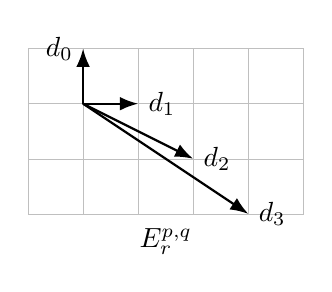
\begin{tikzpicture}[>=Latex, scale=0.7, baseline=(O)]
	\draw[very thin, gray!50]  (-1, 1) grid (4, -2);
	\draw[thick, ->] (0, 0) -- (0, 1) node[left] {$d_0$};
	\draw[thick, ->] (0, 0) -- (1, 0) node[right] {$d_1$};
	\draw[thick, ->] (0, 0) -- (2, -1) node[right] {$d_2$};
	\draw[thick, ->] (0, 0) -- (3, -2) node[right] {$d_3$};
	\node at (1.5, -2.5) {$E_r^{p,q}$};
	\coordinate (O) at (1.5, -0.5);
\end{tikzpicture} \qquad 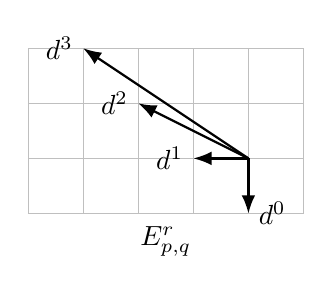
\begin{tikzpicture}[>=Latex, scale=0.7, baseline=(O)]
	\draw[very thin, gray!50]  (1, -1) grid (-4, 2);
	\draw[thick, ->] (0, 0) -- (0, -1) node[right] {$d^0$};
	\draw[thick, ->] (0, 0) -- (-1, 0) node[left] {$d^1$};
	\draw[thick, ->] (0, 0) -- (-2, 1) node[left] {$d^2$};
	\draw[thick, ->] (0, 0) -- (-3, 2) node[left] {$d^3$};
	\node at (-1.5, -1.5) {$E^r_{p,q}$};
	\coordinate (O) at (-1.5, 0.5);
\end{tikzpicture}\end{center}

无论哪种版本, 都可以按照先前的模式来定义 $B_r^p \subset Z_r^p$, $B_r^{p,q} \subset Z_r^{p,q}$, $E_\infty^p$, $E_\infty^{p,q}$ 和 $B^r_p \subset Z^r_p$, $B^r_{p,q} \subset Z^r_{p,q}$, $E^\infty_p$, $E^\infty_{p,q}$ 等对象.

\begin{example}[有限宽的情形]\label{eg:SS-finite-width}
	许多常见场景中, 双分次谱序列的非零项集中在宽度为 $s$ 的水平 (或竖直) 带状区域上, 其中 $s \in \Z_{\geq 0}$, 如下图:
	\[\begin{tikzpicture}[baseline]
		\matrix (M) [matrix of math nodes, right delimiter=\}] {
			\cdots & \bullet & \bullet & \bullet & \cdots \\
			\vdots & \vdots & \vdots & \vdots & \vdots \\
			\cdots & \bullet & \bullet & \bullet & \cdots \\
		};
		\node[right=2em] at (M-2-5) {\scriptsize \text{$s$ 行}};
	\end{tikzpicture} \quad \text{或} \quad \begin{tikzpicture}[baseline]
	\matrix (M) [matrix of math nodes, below delimiter=\}] {
			\vdots & \vdots & \vdots \\
			\bullet & \cdots & \bullet \\
			\bullet & \cdots & \bullet \\
			\vdots & \vdots & \vdots \\
		};
		\node[below=2em] at (M-4-2) {\scriptsize \text{$s$ 列}};
	\end{tikzpicture}\]
	观察箭头走向可见 $r > s$ (或 $r \geq s$) 蕴涵 $d_r^{p,q} = 0$ 对所有 $p, q$ 成立, 此时谱序列在 $E_r$ 页退化. 同调情形类此.
\end{example}

\begin{definition}\label{def:bdd-ss}
	\index{puxulie!有界 (bounded)}
	设 $\mathscr{E}$ 是上同调 (或同调) 双分次谱序列, $r \in \Z$. 若对于每个 $n \in \Z$, 至多仅有有限个 $(p,q) \in \Z^2$ 满足 $p+q=n$ 和 $E_r^{p,q} \neq 0$ (或 $E^r_{p,q} \neq 0$), 则称 $E_r$ (或 $E^r$) \emph{有界}.
\end{definition}

从 $E_{r+1} \simeq \Hm(E_r, d_r)$ 可见 $E_r^{p,q}=0 \implies E_{r+1}^{p,q} = 0$. 特别地, $E_r$ 有界导致 $E_{r+1}$ 有界. 同调情形类此.

\begin{proposition}
	设上同调 (或同调) 双分次谱序列 $\mathscr{E}$ 满足 $E_r$ (或 $E^r$) 有界, 则对于所有 $(p,q) \in \Z^2$, 存在 $r(p,q)$ 使得当 $r \geq r(p,q) \implies E_r^{p,q} = E_{r+1}^{p,q}$ (或 $E^r_{p,q} = E^{r+1}_{p,q}$); 作为推论, $\mathscr{E}$ 的极限存在且满足 $E_r^{p,q} = E_\infty^{p,q}$ (或 $E^r_{p,q} = E^\infty_{p,q}$).
\end{proposition}
\begin{proof}
	讨论 $E_r$ 情形即可. 给定 $n$. 基于有界性质, 当 $r$ 充分大时, 对所有满足 $p+q=n$ 的 $(p,q)$ 都有 $E_r^{p-r, q+r-1} = 0$, 因此 $B_r^{p,q} = 0$. 同理, $r$ 充分大时 $E_r^{p+r, q-r+1} = 0$, 因此 $Z_r^{p,q} = E_r^{p,q}$. 明所欲证.
\end{proof}

\begin{definition}\label{def:quadrant-ss}
	设 $\mathscr{E}$ 是上同调 (或同调) 双分次谱序列, $r \in \Z$. 若 $E_r^{p,q} \neq 0$ (或 $E^r_{p,q} \neq 0$) 蕴涵 $p, q \geq 0$, 则称 $E_r$ (或 $E^r$) 落在第一象限, 类似方法可以定义其他象限的情形.
\end{definition}

落在第一象限或第三象限的 $E_r$ 显然有界. 从 $E_{r+1} \simeq \Hm(E_r, d_r)$ 可见若 $E_r$ 落在第一象限等等, 则 $E_{r+1}$ 亦然. 同调情形类此.

\begin{remark}[边缘计算]\label{rem:edge-computing}
	落在第一象限的谱序列特别常见. 以上同调版本为例, 其边缘项 $E_r^{\bullet ,0}$ 和 $E_r^{0, \bullet}$ 有特殊的性质. 选定 $p, q \geq 1$. 细心探究 $d_r$ 走向, 并且回忆到 $E_{r+1} \simeq \Hm(E_r, d_r)$, 可以验证
	\begin{equation}\label{eqn:edge-ss-coh}\begin{array}{cc}
		E_2^{p,0} \twoheadrightarrow E_3^{p,0} \twoheadrightarrow \cdots \twoheadrightarrow E_{p+1}^{p,0} = E_\infty^{p,0} & \text{($\because$\; 映出的 $d$ 全为 $0$)}, \\
		E_\infty^{0,q} = E_{q+2}^{0,q} \hookrightarrow E_{q+1}^{0,q} \hookrightarrow \cdots \hookrightarrow E_2^{0,q} \hookrightarrow E_1^{0,q} & \text{($\because$\; 映入的 $d$ 全为 $0$)}.
	\end{array}\end{equation}
	落在第一象限的同调双分次谱序列也有对应的性质: 我们有
	\begin{equation}\label{eqn:edge-ss-ho}\begin{array}{cc}
		E^\infty_{p,0} = E^{p+1}_{p,0} \hookrightarrow E^p_{p,0} \hookrightarrow \cdots \hookrightarrow E^3_{p,0} \hookrightarrow E^2_{p,0} & \text{($\because$\; 映入的 $d$ 全为 $0$)}, \\
		E^1_{0,q} \twoheadrightarrow E^2_{0,q} \twoheadrightarrow \cdots \twoheadrightarrow E^{q+2}_{0,q} = E^\infty_{0,q} & \text{($\because$\; 映出的 $d$ 全为 $0$)}.
	\end{array}\end{equation}\index{bianyuantaishe@边缘态射 (edge morphism)}

	来自 \eqref{eqn:edge-ss-coh} 或 \eqref{eqn:edge-ss-ho} 的态射统称为\emph{边缘态射}. 综上可得正合列 ($p \geq 2$)
	\begin{equation}\label{eqn:low-exact-coh}
		0 \to E^{0, p-1}_\infty \to E^{0, p-1}_p \xrightarrow{d} E^{p, 0}_p \to E^{p, 0}_\infty \to 0,
	\end{equation}
	其中除 $d$ 以外的态射都是边缘态射. 正合列也有同调版本 ($p \geq 2$)
	\begin{equation}\label{eqn:low-exact-ho}
		0 \to E^\infty_{p,0} \to E^p_{p,0} \xrightarrow{d} E^p_{0, p-1} \to E^\infty_{0, p-1} \to 0,
	\end{equation}
	初学者请务必动笔写下这些项所涉及的态射 $d$ 的走势, 了解它们何时为 $0$, 从而验证上述所有断言.
\end{remark}

\section{正合偶}\label{sec:exact-couples}
常用的几种谱序列都来自正合偶, 这是 W.\ Massey 的发现. 为了把握问题的实质, 我们先退回不带次数的情形.

\begin{definition}[正合偶]\label{def:exact-couple}
	\index{zhengheou@正合偶 (exact couple)}
	Abel 范畴 $\mathcal{A}$ 上的正合偶意谓 $\mathcal{A}$ 中的正合图表
	\[\begin{tikzcd}[column sep=small]
		D \arrow[rr, "i"] & & D \arrow[ld, "j"] \\
		& E \arrow[lu, "k"] &
	\end{tikzcd}\]
	资料 $\mathscr{C} := (D, E, i, j, k)$ 之间的态射按自明的方式定义.
\end{definition}

给定正合偶 $\mathscr{C} = (D, E, i, j, k)$, 命 $d := jk: E \to E$, 则 $dj = jkj = 0$ 而 $kd = kjk = 0$, 由此可知 $d^2 = 0$. 根据正合条件易得如下分解:
\begin{equation}\label{eqn:exact-couple-aux}
	\begin{tikzcd}
		D \arrow[r, "j"] \arrow[twoheadrightarrow, d, "i"'] & \Ker(d) \arrow[twoheadrightarrow, d] \\
		i(D) \arrow[r, "{\exists! \; j'}"'] & \Hm(E, d)
	\end{tikzcd} \quad \begin{tikzcd}
		\Ker(d) \arrow[r, "k"] \arrow[twoheadrightarrow, d] & i(D) \\
		\Hm(E, d) \arrow[ru, "{\exists! \; k'}"'] &
	\end{tikzcd}
\end{equation}
另外定义 $E' := \Hm(E, d)$, $D' := i(D)$ 和 $i' := i|_{i(D)}: D' \to D'$.

\begin{lemma}
	给定正合偶 $\mathscr{C} = (D, E, i, j, k)$, 按以上方式构造的资料
	\[ \mathscr{C}' = (D', E', i', j', k') : \quad \begin{tikzcd}[column sep=small]
		D' \arrow[rr, "{i'}"] & & D' \arrow[ld, "{j'}"] \\
		& E' \arrow[lu, "{k'}"] &
	\end{tikzcd}\]
	仍是正合偶.
\end{lemma}
\begin{proof}
	细观 \eqref{eqn:exact-couple-aux} 并运用正合条件, 不难验证
	\begin{align*}
		\Ker(i') & = i(D) \cap \Ker(i) = \Ker(j) \cap k(E) \\
		& = \Image\left[ \Ker(d) \xrightarrow{k} i(D) \right] = \Image(k'), \\
		\Ker(j') & = i\left( j^{-1} (jk(E)) \right) \\
		& = i\left( k(E) + \Ker(j) \right) = i\left(i(D)\right) = \Image(i'), \\
		\Ker(k') & = (\Ker(k) \cap \Ker(d))/\Image(d) = (j(D) \cap \Ker(jk)) / \Image(d) \\
		& = j(D) / \Image(d) = \Image(j'). 
	\end{align*}
	所以新的三角图表仍然正合.
\end{proof}

此法迭代, 给出一列正合偶 $(\mathscr{C}_{(r)})_{r \geq 1}$, 使得 $\mathscr{C}_{(1)} = \mathscr{C}$ 而 $r \geq 1$ 时 $\mathscr{C}_{(r+1)} = \mathscr{C}_{(r)}'$. 记 $\mathscr{C}_{(r)} = (D_r, E_r, i_r, j_r, k_r)$, 则 $(E_r, d_r := j_r k_r)_{r \geq 1}$ 给出谱序列.

\begin{lemma}\label{prop:exact-couple-Z-B}
	对于正合偶 $\mathscr{C} = (D, E, i, j, k)$ 得出的谱序列 $(E_r, d_r)_{r \geq 1}$, 按 \eqref{eqn:spectral-sequence-Z-B} 定义 $E = E_1$ 的一族子对象 $\overline{B}_r \subset \overline{Z}_r$; 此处用上划线是因为它们从 $r=1$ 起步, 详见稍后的命题 \ref{prop:differential-exact-couple}. 当 $r \geq 0$ 时
	\begin{gather*}
		\overline{B}_{r+1} = j\left(\Ker(i^r)\right) \subset k^{-1}\left( \Image(i^r) \right) = \overline{Z}_{r+1}; \\
		\overline{B}_\infty = j\left( \bigcup_{r \geq 2} \Ker(i^r) \right) \subset k^{-1}\left( \bigcap_{r \geq 2} \Image(i^r) \right) = \overline{Z}_\infty ,
	\end{gather*}
	前提是所论的 $\bigcup_r$ 和 $\bigcap_r$ 存在. 确切地说, 正合偶 $\mathscr{C}_{(r+1)}$ 典范地同构于
	\[\begin{tikzcd}[column sep=tiny]
		i^r D \arrow[rr, "i"] & & i^r D \arrow[ld, "{\overline{j}_{r+1}}"] \\
		& \dfrac{k^{-1}(i^r D)}{j(\Ker(i^r))} \arrow[lu, "{\overline{k}_{r+1}}"] &
	\end{tikzcd}\]
	其中 $\overline{k}_{r+1}$ 由 $k: E \to D$ 诱导, $\overline{j}_{r+1}$ 则由以下交换图表刻画:
	\[\begin{tikzcd}
		D \arrow[r, "{i^r}"] \arrow[d, "j"'] & i^r D \arrow[d, "{\overline{j}_{r+1}}"] \\
		k^{-1}(i^r D) \arrow[twoheadrightarrow, r] & \dfrac{k^{-1}(i^r D)}{j(\Ker(i^r))}.
	\end{tikzcd}\]
\end{lemma}
\begin{proof}
	关于正合偶 $\mathscr{C}_{(r+1)}$ 的描述可以递归地论证, 其 $r=0$ 情形是平凡的 ($i^0 = \identity$), 而 $\overline{B}_{r+1}$ 和 $\overline{Z}_{r+1}$ 的描述则是其简单推论. 由于细节稍显琐碎, 此处略去. 关于 $\overline{B}_\infty \subset \overline{Z}_\infty$ 的断言由引理 \ref{prop:image-sum-preimage-intersection} (ii) 料理.
\end{proof}

接着说明如何从微分对象构造正合偶.

\begin{proposition}\label{prop:differential-exact-couple}
	设 $\alpha: (D, d) \to (D, d)$ 是 $\mathcal{A}_d$ 的单态射, 记 $d$ 在 $\Coker(\alpha)$ 上诱导的态射为 $d_\alpha$, 则有正合偶:
	\[\begin{tikzcd}[column sep=tiny]
		\Hm(D, d) \arrow[rr, "{i = \Hm(\alpha)}"] & & \Hm(D, d) \arrow[ld, "j"] \\
		& \Hm(\Coker(\alpha), d_\alpha) \arrow[lu, "k"] &
	\end{tikzcd}\]
	取 $\overline{B}_{r+1} \subset \overline{Z}_{r+1}$ 在 $E_0 := \Coker(\alpha)$ 中的逆像, 记为
	\[ 0 =: B_0 \subset B_1 \subset B_2 \subset \cdots \subset Z_2\subset Z_1 \subset Z_0 := \Coker(\alpha). \]
	对于所有 $r \geq 0$, 我们有:
	\begin{itemize}
		\item $B_{r+1}$ 是 $\left(\alpha^r\right)^{-1} (dD) \subset D$ 在 $\Coker(\alpha)$ 中的像;
		\item $Z_{r+1}$ 是 $d^{-1}\left( \alpha^{r+1} D \right) \subset D$ 在 $\Coker(\alpha)$ 中的像;
		\item $d_{r+1} \in \End(Z_{r+1}/B_{r+1})$ 由 $d^{-1} (\alpha^{r+1} D) \xrightarrow{d} \alpha^{r+1} D \xleftarrow[\sim]{\alpha^{r+1}} D$ 诱导.
	\end{itemize}
	特别地, 我们有典范同构
	\[ E_{r+1} \simeq \dfrac{Z_{r+1}}{B_{r+1}} \simeq \dfrac{d^{-1}(\alpha^{r+1} D) + \alpha D}{(\alpha^r)^{-1}(dD) + \alpha D}, \quad r \in \Z_{\geq 1}. \]
\end{proposition}
\begin{proof}
	正合偶是对 $\mathcal{A}_d$ 的短正合列
	\[ 0 \to (D, d) \xrightarrow{\alpha} (D, d) \to (\Coker(\alpha), d_\alpha) \to 0 \]
	施行引理 \ref{prop:diff-obj-triangle} (在其中取 $T = \identity_{\mathcal{A}}$) 的产物; 特别地, 态射 $j$ 由 $D \twoheadrightarrow \Coker(\alpha)$ 诱导, 而 $k$ 的本质是长正合列中的连接态射. 关于 $B_{r+1}$ 的描述无非是引理 \ref{prop:exact-couple-Z-B} 提升到 $E_0$ 的版本. 至于 $Z_{r+1}$, 除了上述引理, 关键还在于描述连接态射 $k: \Hm(\Coker(\alpha), d_\alpha) \to \Hm(D, d)$: 仔细回顾 \eqref{eqn:snake-conn} 和 \eqref{eqn:long-exact-sequence-ses-aux} 的构造, 可知它是由行正合交换图表
	\[\begin{tikzcd}
		& \Coker(d) \arrow[r] \arrow[d, "\overline{d}"'] & \Coker(d) \arrow[r] \arrow[d, "\overline{d}"'] & \Coker(d_\alpha) \arrow[d, "\overline{d_\alpha}"] \arrow[r] & 0 \\
		0 \arrow[r] & \Ker(d) \arrow[r, "\alpha"'] & \Ker(d) \arrow[r] & \Ker(d_\alpha) &
	\end{tikzcd}\]
	的中路 $\overline{d}$ 诱导的, 而 $\overline{d}$ 又来自 $d: D \to D$. 其余验证繁而不难, 读者不妨先从 $\mathcal{A}$ 为模范畴的情形入手.
\end{proof}

微分对象给出的谱序列因此可由 $0$ 起步, 方式是令 $E_0 := \Coker(\alpha)$, $d_0 := d_\alpha$.

对于带平移的 Abel 范畴 $(\mathcal{A}, T)$, 由于带次数的态射依然能作合成, 也同样具备正合性等概念, 正合偶理论容易扩及态射 $i$, $j$, $k$ 带有次数的情形. 以 \S\ref{sec:filtered-diff-ss} 即将探讨的场景为例, 可以考虑正合偶
\[\begin{tikzcd}[column sep=tiny]
	D \arrow[rr, "{-1}"] & & D \arrow[ld, "{+1}"] \\
	& E \arrow[lu] &
\end{tikzcd} \xlongequal{\text{展卷}} \left[
	\begin{tikzcd}[column sep=0ex, every cell/.append style = {font = \small}]
		\cdots & T D \arrow[rr] \arrow[ld] & & D \arrow[rr] \arrow[ld] & & T^{-1} D \arrow[rr] \arrow[ld] & & T^{-2} D \arrow[ld] & \cdots \\
		\cdots & & TE \arrow[lu] & & E \arrow[lu] & & T^{-1} E \arrow[lu] & & \cdots \arrow[lu]
	\end{tikzcd}
\right]. \]
记此正合偶为 $\mathscr{C}$. 引理 \ref{prop:exact-couple-Z-B} 在带次数情形的自然推广表明 $\mathscr{C}_{(r)}$ 形如
$\begin{tikzcd}[column sep=tiny, row sep=small]
	\bullet \arrow[rr, "{-1}"] & & \bullet \arrow[ld, "{+r}"] \\
	& \bullet \arrow[lu] &
\end{tikzcd}$.
所以 $d_r = j_r k_r$ 是 $r$ 次态射. 由此得到的谱序列将是分次的.

\section{滤过微分对象的谱序列}\label{sec:filtered-diff-ss}
本节伊始, 考虑带平移的 Abel 范畴 $(\mathcal{A}, T)$.

\begin{definition}\label{def:filtered-diffop}
	\index{weifenduixiang!滤过 (filtered)}
	配备滤过 $\left(\mathrm{F}^\bullet X, d_{\mathrm{F}^\bullet X}\right)$ 的 $(X, d) \in \Obj((\mathcal{A}, T)_d)$ 称为 $(\mathcal{A}, T)$ 上的\emph{滤过微分对象}. 此时 $\gr^p X$ 也带有自然的 $\gr^p d: \gr^p X \to T \gr^p X$, 使得 $(\gr^p X, \gr^p d) \in \Obj((\mathcal{A}, T)_d)$.
\end{definition}

由于子对象 $\mathrm{F}^p X$ 上的 $d_{\mathrm{F}^p X}$ 宜理解为 $d: X \to T X$ 的限制, 今后仍记之为 $d$. 类似定义可施于升滤过的情形, 表述完全是对偶的.

回到谱序列的研究. 上节介绍了如何从微分对象构造正合偶. 现在考虑 $\mathcal{A}$ 上的滤过微分对象 $(X, d, \mathrm{F}^\bullet X)$. 记 $\mathcal{A}^{\Z}$ 的标准平移函子为 $S: (Y^p)_p \mapsto (Y^{p+1})_p$; 注意到它和对每个 $Y^p$ 作用的 $T$ 当然地交换. 以下探讨的态射因而带两种次数: 一是对应于 $S$  的``滤过次数'', 二是对应于 $T$ 的``内次数'', 暂且聚焦于前者.

滤过既然递降, 遂有单态射
\[ \alpha: \left( \mathrm{F}^{p+1} X, d \right)_{p \in \Z} \hookrightarrow S^{-1} \left( \mathrm{F}^{p+1} X, d \right)_{p \in \Z} = \left( \mathrm{F}^p X, d \right)_{p \in \Z} . \]
 于是 $E_0 := \Coker(\alpha) = \left( \gr^p X, \gr^p d \right)_{p \in \Z}$, 而 $E_1^p = \Hm\left(\gr^p X, \gr^p d\right)$.

将 $\alpha$ 视作 $\mathcal{A}^{\Z}$ 的 $-1$ 次态射 (相对于 $S$), 代入命题 \ref{prop:differential-exact-couple} 得 $\mathcal{A}^{\Z}$ 上带次数的正合偶:
\[\mathscr{C} = \left[ \begin{tikzcd}[column sep=tiny]
	\Hm\left( \mathrm{F}^{p+1} X, d \right)_p \arrow[rr, "-1"', "{\Hm(\alpha)}"] & & \Hm\left( \mathrm{F}^{p+1} X, d \right)_p \arrow[ld, "{+1}"] \\
	& \Hm\left( \gr^p X , \gr^p d \right)_p \arrow[lu] &
\end{tikzcd}\right], \]
此处 $\nwarrow$ 来自短正合列 $0 \to (\mathrm{F}^{p+1} X, d) \to (\mathrm{F}^p X, d) \to (\gr^p X, \gr^p d) \to 0$ 诱导的连接态射.

由此得出的 $\mathscr{E} = (E_r^p, d_r^p)_{\substack{r \geq 0 \\ p \in \Z}}$ 称为 $\mathrm{F}^\bullet X$ 在 $\mathcal{A}^{\Z}$ 中确定的谱序列. 在 \S\ref{sec:exact-couples} 结尾已说明 $d_r$ 相对于 $S$ 是 $r$ 次态射, 表作
\[ d_r = \left( d_r^p : E_r^p \to (S^r E_r)^p = E_r^{p+r} \right)_{p \in \Z}; \]
当然, $d_r$ 的次数也能够从命题 \ref{prop:differential-exact-couple} 的公式读出.

换言之, 滤过微分对象 $(X, d, \mathrm{F}^\bullet X)$ 给出定义 \ref{def:graded-spectral-sequence} 的上同调分次谱序列. 留意到此处的 $d_r^p$ 也可能带内次数 (除非取 $T = \identity_{\mathcal{A}}$), 只是略去不表, 细节待 \S\ref{sec:filtered-cplx-ss} 梳理.

按 \eqref{eqn:spectral-sequence-Z-B} 的方式定义 $Z_0 = (\gr^p X, \gr^p d)_p$ 的子对象
\[ B_r = (B_r^p)_p \subset (Z_r^p)_p = Z_r. \]

为了简化符号, 以下陈述中省略 $d$ 带有的内次数, 这相当于考虑 $T = \identity_{\mathcal{A}}$ 的特例; 推至一般情形是例行公事, 仅须在涉及 $d^{-1}(\cdots)$ 或 $d(\cdots)$ 处适当地插入平移函子, 以使表达式有严格意义.

\begin{proposition}\label{prop:filtered-diff-E}
	给定滤过微分对象 $(X, d, \mathrm{F}^\bullet X)$, 相应的谱序列满足
	\begin{align*}
		Z_r^p & = \dfrac{\left(\mathrm{F}^p X \cap d^{-1} \mathrm{F}^{p+r} X \right) + \mathrm{F}^{p+1} X }{\mathrm{F}^{p+1} X}, \\
		B_r^p & = \dfrac{\left(\mathrm{F}^p X \cap d \mathrm{F}^{p-r+1} X \right) + \mathrm{F}^{p+1} X }{\mathrm{F}^{p+1} X},
	\end{align*}
	而 $d_r^p: E_r^p \to E_r^{p+r}$ 由态射 $d^{-1} \mathrm{F}^{p+r} X \xrightarrow{d} \mathrm{F}^{p+r} X \cap \Ker(d)$ 诱导.
\end{proposition}
\begin{proof}
	留意到 $\alpha^r$ 的 $p$ 次部分可视同嵌入 $\mathrm{F}^p X \hookrightarrow \mathrm{F}^{p-r} X$ 或 $\mathrm{F}^{p+r} X \hookrightarrow \mathrm{F}^p X$. 断言归结为命题 \ref{prop:differential-exact-couple} 的分次版本.
\end{proof}

既然 $\mathcal{A}^{\Z}$ 中的 $\varinjlim$ 和 $\varprojlim$ 是逐次取的, $E_\infty = (E_\infty^p)_{p \in \Z}$ 可以表作
\begin{equation}\label{eqn:filtered-diff-infty}
	E_\infty^p = \dfrac{Z_\infty^p}{B_\infty^p} = \dfrac{\bigcap_r \left( (\mathrm{F}^p X \cap d^{-1} \mathrm{F}^{p+r} X) + \mathrm{F}^{p+1} X \right) }{\bigcup_r \left((\mathrm{F}^p X \cap d \mathrm{F}^{p-r+1} X ) + \mathrm{F}^{p+1} X\right)} ,
\end{equation}
前提是所示之 $\bigcap$ 和 $\bigcup$ 对每个 $p$ 皆存在.

\begin{remark}
	命题 \ref{prop:filtered-diff-E} 对滤过微分对象给出的谱序列是本章后续讨论的基石. 它是正合偶的应用, 但我们也完全可以将命题 \ref{prop:filtered-diff-E} 的公式视为直接定义, 对之验证谱序列所需的一切性质.
\end{remark}

基于以上描述, 可以想见 $(X, d, \mathrm{F}^\bullet X)$ 的谱序列 $E_r^p$ 形似一种逐步逼近 $\Hm(X, d)$ 的过程. 为了明确何谓逼近, 我们需要以下概念.

\begin{definition}[诱导滤过]\label{def:induced-filtration-H}
	\index{lvguo!诱导 (induced)}
	给定 $(\mathcal{A}, T)$ 上的滤过微分对象 $(X, d, \mathrm{F}^\bullet X)$, 则 $\Hm(X,d)$ 带有诱导滤过如下
	\[ \mathrm{F}^p \Hm(X,d) := \Image\left[ \mathrm{F}^p X \cap \Ker(d) \to \Hm(X, d) \right], \quad p \in \Z. \]
\end{definition}

\begin{lemma}\label{prop:induced-filtration-H}
	如果存在 $N$ 使得 $\mathrm{F}^N X = 0$, 则 $\mathrm{F}^N \Hm(X, d) = 0$. 如果 $\mathrm{F}^\bullet X$ 是定义 \ref{def:filtration-properties} 所谓的穷竭滤过, 则 $\mathrm{F}^\bullet \Hm(X, d)$ 亦然.
\end{lemma}
\begin{proof}
	第一部分是平凡的, 以下处理第二部分. 根据引理 \ref{prop:image-sum-preimage-intersection} (ii), $\bigcup_p \mathrm{F}^p \Hm(X,d)$ 是 $\bigcup_p \left( \mathrm{F}^p X \cap \Ker(d) \right)$ 的像, 而由 \eqref{eqn:exhaustion-intersection} 可知
	\[ \bigcup_p \left( \mathrm{F}^p X \cap \Ker(d) \right) = \left(\bigcup_p \mathrm{F}^p X\right) \cap \Ker(d) = \Ker(d). \]
	此外, 若存在 $M$ 使得 $\mathrm{F}^M X = X$, 自然也有 $\mathrm{F}^M \Hm(X, d) = \Hm(X, d)$.
\end{proof}

我们将在 \S\ref{sec:filtered-cplx-ss} 应用这些观察的分次版本.

\begin{lemma}\label{prop:induced-filtration-gr}
	给定滤过微分对象 $(X, d, \mathrm{F}^\bullet X)$, 对每个 $p \in \Z$ 皆有典范同构
	\[ \gr^p \Hm(X, d) \simeq \dfrac{\mathrm{F}^p X \cap \Ker(d)}{ (\mathrm{F}^{p+1} X \cap \Ker(d)) + (\mathrm{F}^p X \cap \Image(T^{-1} d)) }. \]
\end{lemma}
\begin{proof}
	展开 $\mathrm{F}^p \Hm(X,d) / \mathrm{F}^{p+1} \Hm(X,d)$ 的定义, 并且运用 Abel 范畴中标准的同构定理 \ref{prop:Abel-cat-isom-thm} 来推导
	\begin{align*}
		\gr^p \Hm(X, d) & = \dfrac{(\mathrm{F}^p X \cap \Ker(d)) + \Image(T^{-1}d)}{(\mathrm{F}^{p+1} X \cap \Ker(d)) + \Image(T^{-1}d)} \\
		& = \dfrac{(\mathrm{F}^p X \cap \Ker(d)) + (\mathrm{F}^{p+1} X \cap \Ker(d)) + \Image(T^{-1}d)}{(\mathrm{F}^{p+1} X \cap \Ker(d)) + \Image(T^{-1}d)} \\
		& \simeq \dfrac{\mathrm{F}^p X \cap \Ker(d)}{ ((\mathrm{F}^{p+1} X \cap \Ker(d)) + \Image(T^{-1}d)) \cap (\mathrm{F}^p X \cap \Ker(d)) } \\
		& = \dfrac{\mathrm{F}^p X \cap \Ker(d)}{ (\mathrm{F}^{p+1} X \cap \Ker(d)) + (\mathrm{F}^p X \cap \Image(T^{-1} d)) };
	\end{align*}
	最后一步用到 $\mathrm{Sub}_X$ 是模格\footnote{也就是说对于所有满足 $A^\flat \subset A$ 的子对象 $A, A^\flat, B \subset X$ 皆有 $A^\flat + (A \cap B) = (A^\flat + B) \cap A$.} (定理 \ref{prop:subobject-modularity}), $\mathrm{F}^{p+1} X \cap \Ker(d) \subset \mathrm{F}^p X \cap \Ker(d)$ 和 $\Image(T^{-1}d) \subset \Ker(d)$, 其余都是标准的.
\end{proof}

\begin{definition-proposition}\label{def:diff-obj-convergence}
	\index{puxulie!弱收敛, 强收敛 (weakly convergent, strongly convergent)}
	给定滤过微分对象 $(X, d, \mathrm{F}^\bullet X)$, 构造相应的上同调分次谱序列 $(E_r, d_r)_r$, 则在 \eqref{eqn:filtered-diff-infty} 中的 $\bigcap_r$ 和 $\bigcup_r$ 存在的前提下, 极限 $E_\infty$ 存在, 而诱导滤过确定的 $\gr \Hm(X,d)$ 可以典范地实现为 $E_\infty$ 的子商.
	\begin{itemize}
		\item 若 $\gr \Hm(X,d) = E_\infty$, 则称谱序列 $(E_r, d_r)_r$ \emph{弱收敛}.
		\item 若谱序列 $(E_r, d_r)_r$ 弱收敛, $\mathrm{F}^\bullet \Hm(X,d)$ 穷竭而完备, 则称谱序列 $(E_r, d_r)_r$ \emph{强收敛}.
	\end{itemize}
\end{definition-proposition}
\begin{proof}
	固定 $p \in \Z$. 端详 $E_\infty^p$ 的表达式 \eqref{eqn:filtered-diff-infty}, 其分子含 $(\mathrm{F}^p X \cap \Ker(d)) + \mathrm{F}^{p+1} X$, 分母则包含于 $(\mathrm{F}^p X \cap \Image(T^{-1} d)) + \mathrm{F}^{p+1} X$ (回忆到 $d$ 是态射 $X \to TX$). 这就给出 $E_\infty^p$ 的子商
	\begin{multline*}
		\dfrac{(\mathrm{F}^p X \cap \Ker(d)) + \mathrm{F}^{p+1} X}{(\mathrm{F}^p X \cap \Image(T^{-1} d)) + \mathrm{F}^{p+1} X} \\
		\simeq \dfrac{\mathrm{F}^p X \cap \Ker(d)}{ \left( (\mathrm{F}^p X \cap \Image(T^{-1} d)) + \mathrm{F}^{p+1} X \right) \cap \left( \mathrm{F}^p X \cap \Ker(d) \right) } \\
		= \dfrac{\mathrm{F}^p X \cap \Ker(d)}{ (\mathrm{F}^p X \cap \Image(T^{-1} d)) + (\mathrm{F}^{p+1} X \cap \Ker(d)) };
	\end{multline*}
	第一个同构是标准的, 其后的等号用到 $\mathrm{Sub}_X$ 是模格, $\mathrm{F}^p X \cap \Image(T^{-1} d) \subset \mathrm{F}^p X \cap \Ker(d)$ 和 $\mathrm{F}^{p+1} X \subset \mathrm{F}^p X$. 将此代入引理 \ref{prop:induced-filtration-gr}.
\end{proof}

不同文献对收敛的定义略有出入. 一切陈述对于带有升滤过 $(X, d, \mathrm{F}_\bullet X)$ 的微分对象和对应的同调分次谱序列都有对应版本.

\section{滤过复形的谱序列}\label{sec:filtered-cplx-ss}
\index{fuxing!滤过 (filtered)}
\index{puxulie!滤过复形的}

延续 \S\ref{sec:filtered-diff-ss} 的思路, 仍选定 Abel 范畴 $\mathcal{A}$. 命题 \ref{prop:filtered-diff-E} 关于滤过微分对象的结论可以进一步推广, 容许态射 $d$ 带有次数. 特别地, 这套理论可以用于滤过复形.

具体言之, 以 $\mathcal{A}^{\Z}$ 代替原先的 $\mathcal{A}$, 其上的平移函子记为 $T$. 根据例 \ref{eg:cplx-as-diff}, $\left(\mathcal{A}^{\Z}, T \right)_d$ 的对象 $(X, d)$ 可以视同复形 $X \in \Obj(\cate{C}(\mathcal{A}))$; 进一步考虑降滤过 $(X, d, \mathrm{F}^\bullet X)$, 则
\begin{align*}
	\Hm(X, d) & = \left( \Hm^n(X) \right)_{n \in \Z}, \\
	\Hm\left( \mathrm{F}^p X, d \right) & = \left( \Hm^n\left(\mathrm{F}^p X\right)\right)_{n \in \Z}, \\
	\mathrm{F}^p \Hm^n(X) &:= \Image\left[ \mathrm{F}^p X^n \cap \Ker\left(d_X^n\right) \to \Hm^n(X) \right] \quad \text{(定义 \ref{def:induced-filtration-H}).}
\end{align*}

综之, 先前构造的谱序列 $\mathscr{E}$ 中的 $E_r$ 实则取值在 $\mathcal{A}^{\Z \times \Z}$, 它是双分次对象: 除了滤过次数 $p$, 另有关乎复形结构的``内次数'' $n$, 两者对应的平移函子 $S$ 和 $T$ 严格交换. 已知 $d_r$ 对 $S$ 的次数为 $r$, 以下来探讨它对 $T$ 的次数.

\begin{itemize}
	\item 在用来构造 $\mathscr{E}$ 的正合偶 $\mathscr{C}_{(1)}$ 中, 态射 $\nwarrow$ 相对于 $T$ 是 $1$ 次的, 其余皆零次: 诚然, $\nwarrow$ 来自上同调的连接态射, 故对 $T$ 是 $1$ 次态射, 而其余箭头易见为零次.
	\item 运用引理 \ref{prop:exact-couple-Z-B} 的描述, 可递归地推得以上陈述也适用于一般的 $\mathscr{C}_{(r)}$.
	\item 作为推论, $d_r$ 和 $(X, d)$ 中的 $d$ 对 $T$ 同样是 $1$ 次态射. 这点也可以直接从命题 \ref{prop:differential-exact-couple} 的描述一眼看穿.
\end{itemize}

基于应用考量, 惯例是改用 $p$ 和 $q := n-p$ 来标号, 于是
\begin{gather*}
	E_r = (E_r^{p,q})_{(p,q) \in \Z^2} = \left( Z_r^{p,q} / B_r^{p,q} \right)_{(p,q) \in \Z^2}, \\
	E_0^{p,q} = \left( \gr^p X \right)^{p+q}, \\
	E_1^{p,q} = \Hm^{p+q}\left( \gr^p X, \gr^p d \right), \\
	d_r = \left( d_r^{p,q}: E_r^{p,q} \to E_r^{p+r, q-r+1} \right)_{(p,q) \in \Z^2}: E_r \xrightarrow{(r, -r+1)} E_r.
\end{gather*}
换言之, 滤过复形给出定义 \ref{def:graded-spectral-sequence} 的上同调双分次谱序列. 对偶地, 带有升滤过的链复形给出同调双分次谱序列.

\begin{example}\label{eg:canonically-bdd-ss}
	考虑滤过复形 $(X, d, \mathrm{F}^\bullet X)$. 若对所有 $n \in \Z$ 都有 $\mathrm{F}^0 X^n = X^n$ 和 $\mathrm{F}^{n+1} X^n = 0$, 则 $E_0$ 落在第一象限 (定义 \ref{def:quadrant-ss}): 这是 $E_0^{p,q} = \left(\gr^p X \right)^{p+q}$ 的直接结论.
\end{example}

\begin{proposition}\label{prop:filtered-cplx-ss}
	给定带有降滤过 $\mathrm{F}^\bullet X$ 的复形 $X \in \Obj(\cate{C}(\mathcal{A}))$, 相应的谱序列满足
	\begin{align*}
		Z_r^{p,q} & = \dfrac{\left(\mathrm{F}^p X^{p+q} \cap d^{-1} \mathrm{F}^{p+r} X^{p+q+1} \right) + \mathrm{F}^{p+1} X^{p+q} }{\mathrm{F}^{p+1} X^{p+q}}, \\
		B_r^{p,q} & = \dfrac{\left(\mathrm{F}^p X^{p+q} \cap d \mathrm{F}^{p-r+1} X^{p+q-1} \right) + \mathrm{F}^{p+1} X^{p+q} }{\mathrm{F}^{p+1} X^{p+q}},
	\end{align*}
	而 $d_r^{p,q}: E_r^{p,q} \to E_r^{p+r, q-r+1}$ 由 $d^{-1} \mathrm{F}^{p+r} X^{p+q+1} \xrightarrow{d} \mathrm{F}^{p+r} X^{p+q+1} \cap \Ker(d)$ 诱导.
\end{proposition}
\begin{proof}
	在命题 \ref{prop:filtered-diff-E} 中计入复形的次数 $n = p+q$, 并留意 $d$ 对复形的平移函子 $T$ 是 $1$ 次态射.
\end{proof}

同理, \eqref{eqn:filtered-diff-infty} 有双分次版本
\begin{equation}\label{eqn:filtered-cplx-infty}
	E_\infty^{p,q} = \dfrac{Z_\infty^{p,q}}{B_\infty^{p,q}} = \dfrac{\bigcap_r \left( (\mathrm{F}^p X^{p+q} \cap d^{-1} \mathrm{F}^{p+r} X^{p+q+1}) + \mathrm{F}^{p+1} X^{p+q} \right) }{\bigcup_r \left((\mathrm{F}^p X^{p+q} \cap d \mathrm{F}^{p-r+1} X^{p+q-1} ) + \mathrm{F}^{p+1} X^{p,q} \right)} ,
\end{equation}
前提是所示的 $\bigcup$ 和 $\bigcap$ 存在; 此时 $E_\infty = (E_\infty^{p,q})_{(p,q) \in \Z^2}$.

定义--命题 \ref{def:diff-obj-convergence} 在此化为双分次版本: $\gr^p \Hm^{p+q}(X)$ 对所有 $p, q$ 皆典范地实现为 $E_\infty^{p,q}$ 的子商. 谱序列的收敛性质也相应地细化.

\begin{definition}\label{def:filtered-cplx-convergence}
	\index{puxulie!弱收敛, 强收敛 (weakly convergent, strongly convergent)}
	对 $\mathcal{A}$ 上的滤过复形 $(X, d, \mathrm{F}^\bullet X)$ 构造相应的上同调分次谱序列 $(E_r, d_r)_r$, 则在 \eqref{eqn:filtered-cplx-infty} 中的 $\bigcap_r$ 和 $\bigcup_r$ 存在的前提下, $\gr^p \Hm^{p+q}(X)$ 可以典范地实现为 $E_\infty^{p,q}$ 的子商.
	\begin{itemize}
		\item 若对所有 $(p,q) \in \Z^2$ 皆有 $\gr^p \Hm^{p+q}(X) = E_\infty^{p,q}$, 则称谱序列 $(E_r, d_r)_r$ \emph{弱收敛}.
		\item 在弱收敛的前提下, 若对所有 $n \in \Z$, 滤过 $\mathrm{F}^\bullet \Hm^n(X)$ 穷竭而完备, 则称谱序列 $(E_r, d_r)_r$ \emph{强收敛}.
	\end{itemize}
\end{definition}

\begin{convention}\label{con:ss-conv}
	\index[sym1]{Erpq abuts to H@$E_r^{p,q} \Rightarrow \Hm^{p+q} (X)$}
	谱序列的强收敛也记为 $E_r^{p,q} \Rightarrow \Hm^{p+q} (X)$; 此处的下标 $r$ 常具体写作 $1$, $2$ 等, 取决于我们着重描述谱序列的哪一页.
	
	推而广之, 若有上同调双分次谱序列 $\mathscr{E}$, 滤过分次对象 $(H, \mathrm{F}^\bullet H)$ 连同同构 $E_\infty^{p,q} \simeq \gr^p H^{p+q}$, 而且 $\mathrm{F}^\bullet H$ 穷竭而完备, 则我们也将此情境标记为 $E_r^{p, q} \Rightarrow H^{p+q}$. 同调双分次谱序列的情形依此类推, 特别地, $E^r_{p, q} \Rightarrow H_{p+q}$ 蕴涵 $E^\infty_{p,q} \simeq \gr_p H_{p+q}$.
\end{convention}

以下的经典收敛定理对于初步应用已经足够. 更广的收敛条件可参见 \cite{Boa99}.

\begin{theorem}[经典收敛定理]\label{prop:classical-convergence}
	考虑滤过复形 $(X, d, \mathrm{F}^\bullet X)$. 假定对于每个 $n \in \Z$,
	\begin{compactitem}
		\item 滤过 $\mathrm{F}^\bullet X^n$ 是穷竭的 (定义 \ref{def:filtration-properties}),
		\item 存在 $N = N(n)$ 使得 $\mathrm{F}^N X^n = 0$,
	\end{compactitem}
	则相应的谱序列强收敛 (定义--命题 \ref{def:diff-obj-convergence}).
	
	如果将条件强化为每个 $X^n$ 的滤过皆有限 (定义 \ref{def:filtration}), 则 $\Hm^n(X)$ 上的诱导滤过也有限. 此时相应的谱序列有界 (定义 \ref{def:bdd-ss}).
\end{theorem}
\begin{proof}
	基于引理 \ref{prop:induced-filtration-H}, 确切地说是其分次版本, 诱导滤过 $\mathrm{F}^\bullet \Hm^n(X)$ 穷竭而完备. 问题归结为证弱收敛.
	
	有必要回顾定义--命题 \ref{def:diff-obj-convergence} 的证明, 它说明如何对每个 $(p,q) \in \Z^2$ 将 $\gr^p \Hm^{p+q}(X)$ 实现为 $E_\infty^{p,q}$ 的子商: 关键是
	\begin{equation*}\begin{split}
		\bigcap_r & \left( \left( \mathrm{F}^p X^{p+q} \cap d^{-1} \mathrm{F}^{p+r} X^{p+q+1} \right) + \mathrm{F}^{p+1} X^{p+q} \right) \\
		& \supset \left( \mathrm{F}^p X^{p+q} \cap \Ker(d) \right) + \mathrm{F}^{p+1} X^{p+q}, \\
		\bigcup_r & \left( \left( \mathrm{F}^p X^{p+q} \cap d\mathrm{F}^{p-r+1} X^{p+q-1} \right) + \mathrm{F}^{p+1} X^{p+q} \right) \\
		& \subset \left( \mathrm{F}^p X^{p+q} \cap \Image(d) \right) + \mathrm{F}^{p+1} X^{p+q}.
	\end{split}\end{equation*}
	证明谱序列弱收敛相当于将这些包含关系改进为等号. 然而, 当 $r \gg 0$ (相对于 $p, q$) 时, 第一式的 $\bigcap_r$ 内部无非是 $\left( \mathrm{F}^p X^{p+q} \cap \Ker(d) \right) + \mathrm{F}^{p+1} X^{p+q}$, 故等号成立.

	对于第二式, 可以先将 $+ \mathrm{F}^{p+1} X^{p+q}$ 移出 $\bigcup_r$. 回忆到 $d(\mathrm{F}^\bullet X^n)$ 必为 $d(X^n)$ 的穷竭滤过, 故
	\begin{multline*}
		\bigcup_r \left( \mathrm{F}^p X^{p+q} \cap d\mathrm{F}^{p-r+1} X^{p+q-1} \right) \\
		\xlongequal{\because\; \text{\eqref{eqn:exhaustion-intersection}}} \mathrm{F}^p X^{p+q} \cap \bigcup_r d\mathrm{F}^{p-r+1} X^{p+q-1} \\
		= \mathrm{F}^p X^{p+q} \cap d \bigcup_r \mathrm{F}^{p-r+1} X^{p+q-1}
		= \mathrm{F}^p X^{p+q} \cap \Image(d).
	\end{multline*}

	最后假定每个 $X^n$ 的滤过皆有限, 这时 $\mathrm{F}^\bullet \Hm^n(X)$ 自然有界. 以下说明谱序列有界. 选定 $r$ 和 $n$, 设 $p+q=n$. 根据命题 \ref{prop:filtered-cplx-ss} 的描述, $p \gg 0$ 时 $Z_r^{p,q}$ 的分子为 $0$, 而 $p \ll 0$ 时分母为 $X^n$. 由此可见至多仅有有限个 $(p,q)$ 使得 $E_{r+1}^{p,q} \neq 0$.
\end{proof}

对偶版本不言自明, 此处不再重复.

\begin{corollary}[低次项的正合列]\label{prop:low-degree-ss}
	设滤过复形 $(X, d, \mathrm{F}^\bullet X)$ 满足
	\[ \mathrm{F}^0 X^n = X^n, \quad \mathrm{F}^{n+1} X^n = 0, \quad n \in \Z, \]
	如例 \ref{eg:canonically-bdd-ss}. 对应的谱序列给出典范正合列
	\[ 0 \to E_2^{1,0} \to \Hm^1(X) \to E_2^{0,1} \xrightarrow{d} E_2^{2, 0} \to \Hm^2(X). \]
	对于带升滤过的链复形 $X$, 若 $\mathrm{F}_{-1} X = 0$ 而 $\mathrm{F}^n X = X$, 则对偶地有典范正合列
	\[ \Hm_2(X) \to E^2_{2,0} \xrightarrow{d} E^2_{0,1} \to \Hm_1(X) \to E^2_{1,0} \to 0. \]
\end{corollary}
\begin{proof}
	在 \eqref{eqn:low-exact-coh} 代入 $p=2$, 得到正合列
	\[ 0 \to E_\infty^{0,1} \to E_2^{0,1} \xrightarrow{d} E_2^{2, 0} \to E_\infty^{2,0} \to 0. \]
	基于经典收敛定理 \ref{prop:classical-convergence}, 我们有 $E_\infty^{0,1} \simeq \gr^0 \Hm^1(X)$, $E_\infty^{1, 0} \simeq \gr^1 \Hm^1(X)$ 和 $E_\infty^{2, 0} \simeq \gr^2 \Hm^2(X)$. 根据条件,
	\begin{gather*}
		\gr^2 \Hm^2(X) = \mathrm{F}^2 \Hm^2(X), \quad \gr^1 \Hm^1(X) = \mathrm{F}^1 \Hm^1(X), \\
		\gr^0 \Hm^1(X) = \Hm^1(X) / \mathrm{F}^1 \Hm^1(X) = \Hm^1(X) / E_\infty^{1,0}.
	\end{gather*}
	此外, 对 \eqref{eqn:edge-ss-coh} 代入 $p=1$ 给出 $E_2^{1,0} = E_\infty^{1,0}$. 这些等式拼接为所求的正合列. 同调版本不赘.
\end{proof}

在 $E_r^{p,q}$ 强收敛的前提下, 一旦掌握足够多个 $(E_r, d_r)$, 原则上便能从 $E_\infty$ 读出 $\left( \gr^p \Hm^{p+q}(X) \right)_{p,q \in \Z}$. 然而从 $(\gr^p \Hm^n(X))_p$ 过渡到 $\Hm^n(X)$ 相当于在 $\mathcal{A}$ 中确定一系列扩张; 除非 $\Hm^n(X)$ 分裂, 一般不易处理. 如果我们仅考量较粗糙的性质, 则谱序列有时能提供简洁的答案. 以下阐释的例子本质上是 Euler--Poincaré 原理的应用.

\begin{lemma}\label{prop:finite-degeneration}
	设 $\mathscr{E} = (E_r, d_r)_{r \geq 1}$ 是上同调双分次谱序列, 而且存在 $r$ 使得
	\[ \left\{ (p,q) \in \Z^2 : E_r^{p,q} \neq 0 \right\} \quad \text{是有限集}, \]
	则当 $r \gg 0$ 时 $\mathscr{E}$ 在 $E_r$ 页退化.
\end{lemma}
\begin{proof}
	由条件知 $r$ 足够大时 $E_r$ 的非零项集中在一个长宽皆有限的区域. 代入例 \ref{eg:SS-finite-width}.
\end{proof}

\begin{proposition}\label{prop:EP-ss}
	设上同调双分次谱序列 $(E_r, d_r)_r$ 满足以下条件:
	\begin{compactitem}
		\item 存在 $r$ 使得 $\left\{ (p,q) \in \Z^2 : E_r^{p,q} \neq 0 \right\}$ 是有限集,
		\item 强收敛性 $E_r^{p, q} \Rightarrow H^{p+q}$, 含义如约定 \ref{con:ss-conv},
	\end{compactitem}
	则在定义 \ref{def:K0} 的群 $\mathrm{K}_0(\mathcal{A})$ 中, 当 $r \gg 0$ 时等式
	\[ \sum_{n \in \Z} (-1)^n \left[ H^n \right] = \sum_{p, q \in \Z} (-1)^{p+q} \left[ E_r^{p,q} \right] \]
	成立, 两边都是有限和.
\end{proposition}
\begin{proof}
	当 $r \gg 0$ 时, 右式的和仅有有限项非零. 此外,
	\[ E_{r+1}^{p,q} \simeq \Hm\left[ E_r^{p-r, q+r-1} \xrightarrow{d} E_r^{p,q} \xrightarrow{d} E_r^{p+r, q-r+1} \right] \]
	按 $n := p+q$ 来统计次数, 则 $d$ 是次数为 $1$ 的态射. 在 $\mathrm{K}_0(\mathcal{A})$ 当中对 $n$ 取交错和, 然后应用定理 \ref{prop:EP} 得到
	\[ \sum_{p, q \in \Z} (-1)^{p+q} \left[ E_r^{p,q} \right] = \sum_{p, q \in \Z} (-1)^{p+q} \left[ E_{r+1}^{p,q} \right]. \]
	
	引理 \ref{prop:finite-degeneration} 说明谱序列终归退化, 因此当 $r \gg 0$ 时 $E_r^{p,q} = E_\infty^{p,q}$ 对所有 $(p, q)$ 成立. 于是 $r \gg 0$ 时
	\[ \sum_{p,q} (-1)^{p+q} \left[ E_r^{p,q} \right] = \sum_{p,q} (-1)^{p+q} \left[ \gr^p \Hm^{p+q}(X) \right] = \sum_n (-1)^n \sum_p \left[ \gr^p H^n \right], \]
	条件确保求和皆有限. 而按引理 \ref{prop:K0-prep} (v) 和 $\mathrm{F}^\bullet H$ 的条件, 我们又有 $\sum_p \left[ \gr^p H^n(X) \right] = \left[ \Hm^n(X) \right]$.
\end{proof}

若 $(E_r, d_r)_r$ 来自滤过复形 $(X, d, \mathrm{F}^\bullet)$, 而且每个 $X^n$ 的滤过 $\mathrm{F}^\bullet X^n$ 皆有限, 则定理 \ref{prop:classical-convergence} 确保命题 \ref{prop:EP-ss} 的强收敛条件 $E_r^{p,q} \Rightarrow \Hm^{p+q}(X)$ 自动成立, 但关于 $\{ (p,q) : E^{p, q}_r \neq 0\}$ 的条件则并非自动的.

滤过复形已经足以产出一些简单而有用的谱序列, 见本章习题. 本书的主题是代数学, 其中最广为人知的几种谱序列都来自双复形, 是以我们先转向双复形的情形.

\section{双复形的谱序列及其应用}\label{sec:double-cplx-ss}
\index{puxulie!双复形的}
以下总默认 Abel 范畴 $\mathcal{A}$ 具备所论的可数直和或可数积. 设 $X$ 是 $\mathcal{A}$ 上的双复形, 写作 $X \in \Obj(\cate{C}^2(\mathcal{A}))$. 全复形 $\tot_{\oplus} X$ 具有两种降滤过
\begin{align*}
	\mathrm{F}^p_{\mathrm{I}} (\tot_{\oplus} X)^n & = \bigoplus_{\substack{i+j=n \\ i \geq p}} X^{i, j}, \\
	\mathrm{F}^q_{\mathrm{II}} (\tot_{\oplus} X)^n & = \bigoplus_{\substack{i+j=n \\ j \geq q}} X^{i, j} .
\end{align*}
对每个 $(i, j)$ 分量个别地考察, 可见
\[ \bigcap_p \mathrm{F}^p_{\mathrm{I}} = 0 = \bigcap_q \mathrm{F}^q_{\mathrm{II}}, \quad \bigcup_p \mathrm{F}^p_{\mathrm{I}} = \tot_{\oplus} X = \bigcup_q \mathrm{F}^q_{\mathrm{II}}. \]

由此得到滤过复形, 对应的谱序列分别记为 $\mathscr{E}_{\mathrm{I}} = \mathscr{E}_{\mathrm{I}}(X)$ 和 $\mathscr{E}_{\mathrm{II}} = \mathscr{E}_{\mathrm{II}}(X)$, 或更具体地记为 $E_{\mathrm{I}, r}^{p,q}$ 和 $E_{\mathrm{II}, r}^{p,q}$, 其中 $r \in \Z_{\geq 0}$. 假如 $X^{p,q} \neq 0 \implies p,q \geq 0$, 这时我们称 $X$ 落在第一象限, 则对于 $\star \in \{ \mathrm{I}, \mathrm{II} \}$, 我们有
\[ \mathrm{F}_\star^0 \left(\tot_{\oplus} X \right)^n = \left(\tot_{\oplus} X\right)^n, \quad \mathrm{F}_\star^{n+1} \left(\tot_{\oplus} X \right)^n = 0 , \]
相应的谱序列因而也落在第一象限.

对于链双复形 $X$, 同样可定义两种升滤过
\begin{align*}
	\mathrm{F}_{\mathrm{I}, p} \left( \tot_{\oplus} X \right)_n & = \bigoplus_{\substack{i+j=n \\ i \leq p}} X_{i, j}, \\
	\mathrm{F}_{\mathrm{II}, q} \left( \tot_{\oplus} X \right)_n & = \bigoplus_{\substack{i+j=n \\ j \leq q}} X_{i, j},
\end{align*}
以及对应的同调双分次谱序列.

\begin{proposition}\label{prop:double-cplx-ss}
	对于 $X \in \Obj(\cate{C}^2(\mathcal{A}))$, 其谱序列的前几页和相应的态射 $d$ 有如下描述
	\[\begin{array}{|c|c|c|c|c|c|} \hline
		& E_0^{p,q} & d_0^{p,q} & E_1^{p,q} & d_1^{p,q} & E_2^{p,q} \\ \hline
		\mathscr{E}_{\mathrm{I}} & X^{p,q} & (-1)^p \dvert^{p,q} & \Hm^q(X^{p, \bullet}, \dvert) & \Hm^q(\dhori^{p, \bullet}) & \Hm_{\mathrm{I}}\Hm_{\mathrm{II}}(X)^{p,q} \\
		\mathscr{E}_{\mathrm{II}} & X^{q,p} & \dhori^{q,p} & \Hm^q(X^{\bullet, p}, \dhori) & (-1)^q \Hm^q(\dvert^{\bullet, p}) & \Hm_{\mathrm{II}} \Hm_{\mathrm{I}}(X)^{q,p} \\ \hline
	\end{array}\]
	函子 $\Hm_{\mathrm{I}}, \Hm_{\mathrm{II}}: \cate{C}^2(\mathcal{A}) \to \cate{C}^2(\mathcal{A})$ 的定义见诸 \S\ref{sec:double-cplx-coh}, 特别是 \eqref{eqn:HIHII}.
	
	对于链复形及其同调, 类似方法可得下表.
	\[\begin{array}{|c|c|c|c|c|c|} \hline
		& E^0_{p,q} & d^0_{p,q} & E^1_{p,q} & d^1_{p,q} & E^2_{p,q} \\ \hline
		\mathscr{E}_{\mathrm{I}} & X_{p,q} & (-1)^p \dvert_{p,q} & \Hm_q(X_{p, \bullet}, \dvert) & \Hm_q(\dhori_{p, \bullet}) & \Hm_{\mathrm{I}}\Hm_{\mathrm{II}}(X)_{p,q} \\
		\mathscr{E}_{\mathrm{II}} & X_{q,p} & \dhori_{q,p} & \Hm_q(X_{\bullet, p}, \dhori) & (-1)^q \Hm_q(\dvert_{\bullet, p}) & \Hm_{\mathrm{II}} \Hm_{\mathrm{I}}(X)_{q,p} \\ \hline
	\end{array}\]
\end{proposition}
\begin{proof}
	这是按命题 \ref{prop:filtered-cplx-ss} 的描述循规蹈矩地验证的结果, $\dvert$ 所带正负号来自全复形的定义. 细节不赘.
\end{proof}

这些定义和结果对 $\tot_{\Pi} X$ 也可以如法炮制, 性质完全类似.

对于 $X \in \Obj(\cate{C}^2_f(\mathcal{A}))$ (定义 \ref{def:Cf-Supp}), 其全复形仅涉及有限直和, 不必区分 $\oplus$ 和 $\Pi$ 两种版本, 统一记为 $\tot X$.

\begin{theorem}\label{prop:tot-ss}
	设 $X \in \Obj(\cate{C}^2_f(\mathcal{A}))$, 则相应的两个谱序列 $\mathscr{E}_{\mathrm{I}}$ 和 $\mathscr{E}_{\mathrm{II}}$ 皆有界, 强收敛, 而 $\Hm^n(\tot X)$ 上对应的两个诱导滤过对每个 $n \in \Z$ 皆有限.
\end{theorem}
\begin{proof}
	从 $\cate{C}^2_f(\mathcal{A})$ 的定义可见 $\mathrm{F}_{\mathrm{I}}^\bullet \left( \tot X \right)^n$ 和 $\mathrm{F}_{\mathrm{II}}^\bullet \left( \tot X \right)^n$ 对每个 $n$ 都是有限滤过. 代入定理 \ref{prop:classical-convergence}.
\end{proof}

以下介绍具有代表性的几个应用. 由于涉及的滤过和谱序列总是有限, 这些结果适用于一切 Abel 范畴\footnote{稍加精确地说, 极限项 $Z_\infty^{p,q}$, $B_\infty^{p,q}$, $E_\infty^{p,q}$ 的存在性和定义 \ref{def:filtration-properties} 关于穷竭滤过的条件都不成问题.}.

\begin{example}\label{eg:double-cplx-tot-ss}
	今以谱序列重证定理 \ref{prop:double-cplx-tot}: 若 $\cate{C}^2_f(\mathcal{A})$ 的态射 $f: X \to Y$ 诱导 $\Hm_{\mathrm{II}} \Hm_{\mathrm{I}}(X) \rightiso \Hm_{\mathrm{II}}\Hm_{\mathrm{I}}(Y)$ (或 $\Hm_{\mathrm{I}} \Hm_{\mathrm{II}}(X) \rightiso \Hm_{\mathrm{I}}\Hm_{\mathrm{II}}(Y)$), 则 $\tot(f): \tot(X) \to \tot(Y)$ 是拟同构.
	
	首先设 $\Hm_{\mathrm{II}} \Hm_{\mathrm{I}}(X) \rightiso \Hm_{\mathrm{II}}\Hm_{\mathrm{I}}(Y)$; 由 $f$ 诱导谱序列的态射 $\mathscr{E}_{\mathrm{II}}(X) \to \mathscr{E}_{\mathrm{II}}(Y)$. 它在 $E_2$ 页已经是同构, 于是在极限页 $E_\infty$ 也给出同构 (命题 \ref{prop:ss-isom-infty}).

	基于定理 \ref{prop:tot-ss} 确保的收敛性, $\tot(f)$ 给出的 $\gr^p \left( \Hm^n \tot(X) \right) \to \gr^p\left( \Hm^n \tot(Y) \right)$ 对所有 $p, n \in \Z$ 都是同构. 已知 $\Hm^n$ 上的诱导滤过有限, 故 $\Hm^n \tot(f): \Hm^n \tot(X) \to \Hm^n \tot(Y)$ 也是同构 (命题 \ref{prop:gr-isom}).
	
	若考虑谱序列 $\mathscr{E}_{\mathrm{I}}$, 则可相应地从 $\Hm_{\mathrm{I}} \Hm_{\mathrm{II}}(X) \rightiso \Hm_{\mathrm{I}}\Hm_{\mathrm{II}}(Y)$ 推导 $\tot(f)$ 是拟同构.
\end{example}

\begin{example}[双函子求导]\label{eg:bifunctor-ss}
	设 Abel 范畴 $\mathcal{A}_1$ 和 $\mathcal{A}_2$ 有足够的内射对象 (或投射对象), 而双函子 $F: \mathcal{A}_1 \times \mathcal{A}_2 \to \mathcal{B}$ 对每个变元都左正合 (或右正合). 以下举左正合情形为例. 设 $X_i \in \Obj(\mathcal{A}_i)$ 并选定内射解消 $0 \to X_i \to I_i^0 \to \cdots$; 当 $n < 0$ 时命 $I_i^n := 0$ (其中 $i = 1, 2$). 以此构造落在第一象限的双复形
	\[ Y^{p, q} := F\left( I_1^p, I_2^q \right). \]
	对应的第一象限谱序列 $\mathscr{E}_{\mathrm{I}}$ 因而满足
	\[ E_1^{p,q} = \Hm^q\left( F(I_1^p, I_2^\bullet) \right) \Rightarrow \Hm^{p+q}(\tot(Y)), \quad p,q \in \Z. \]
	右式的 $\Hm^{p+q}(\tot Y)$ 是右导出双函子的取值 $\mathrm{R}^{p+q} F(X_1, X_2)$, 请见定义 \ref{def:derived-bifunctor}.
	
	现在进一步要求 $F$ 是平衡的 (定义 \ref{def:balanced-functor}); 因此 $F(I_1^p, \cdot)$ 是正合函子. 这说明 $q \neq 0 \implies E_1^{p,q} = 0$ 而 $E_1^{p,0} = F(I_1^p, X_2)$. 由此可见 $q \neq 0 \implies E_2^{p,q} = 0$, 而
	\begin{align*}
		E_2^{p,0} & = \Hm^p\left[ \cdots \to F(I_1^p, X_2) \to F(I_1^{p+1}, X_2) \to \cdots \right] \\
		& = (\mathrm{R}_{\mathrm{I}}^p F)(X_1, X_2), \quad \text{符号如定理 \ref{prop:balanced-primer}}.
	\end{align*}
	特别地, 谱序列在 $E_2$ 页退化, 导致
	\begin{align*}
		E_2^{p,q} & = E_\infty^{p,q}, \\ 
		E_\infty^{p,q} & = \gr^p \Hm^{p+q}\left(\tot(Y)\right) = 0, \quad \text{如果}\; q \neq 0, \\
		E_\infty^{p,0} & = \Hm^p\left(\tot(Y)\right) = \mathrm{R}^p F(X_1, X_2) .
	\end{align*}
	这就给出了 $\mathrm{R}^n F(X_1, X_2) \simeq (\mathrm{R}_{\mathrm{I}}^n F)(X_1, X_2)$. 若改用 $\mathscr{E}_{\mathrm{II}}$, 同理可得 $\mathrm{R}^n F(X_1, X_2) \simeq (\mathrm{R}_{\mathrm{II}}^n F)(X_1, X_2)$. 于是 $\mathrm{R}_{\mathrm{I}} F \simeq \mathrm{R}_{\mathrm{II}} F$; 这正是定理 \ref{prop:balanced-primer} 的陈述.
\end{example}

\begin{example}[超导出函子的谱序列]\label{eg:hyperderived-ss}
	\index{chaodaochuhanzi}
	\index{puxulie!超导出函子的}
	设 $\mathcal{A}$ 和 $\mathcal{B}$ 是 Abel 范畴, $\mathcal{A}$ 有足够的内射对象 (或投射对象), 而 $F: \mathcal{A} \to \mathcal{B}$ 是左正合 (或右正合) 加性函子. 我们在 \S\ref{sec:derived-primer} 的前半部对复形 $X \in \Obj(\cate{C}^+(\mathcal{A}))$ (或 $X \in \Obj(\cate{C}^-(\mathcal{A}))$) 定义了右导出函子 $\mathrm{R}^n F(X)$ (或左导出函子 $\mathrm{L}_n F(X)$), 其中 $n \in \Z$. 当 $X \in \Obj(\mathcal{A})$ 时, 它们是经典意义下的导出函子; 与此相对, 一般复形的情形则习惯称为超导出函子. 两者可由谱序列相联系. 以下阐述右导出函子的情形, 上下标对调便是左导出函子的版本.

	设 $X \in \Obj(\cate{C}^+(\mathcal{A}))$. 将 $X$ 视同集中在第 $0$ 行的双复形, 再取定理 \ref{prop:CE-resolution} 提供的 Cartan--Eilenberg 解消 $\epsilon: X \to I$; 这是 $\cate{C}^2_f(\mathcal{A})$ 的态射. 根据注记 \ref{rem:double-cplx-resolution} 或者例 \ref{eg:double-cplx-tot-ss} 的结果, $\tot(\epsilon): X = \tot(X) \to \tot(I)$ 是 $\cate{C}^+(\mathcal{A})$ 中的拟同构, 因而是 $X$ 的内射解消.
	
	从双复形 $(\cate{C}^2 F)(I) \in \Obj\left(\cate{C}^2_f(\mathcal{B})\right)$ 构造收敛谱序列 $\mathscr{E}_{\mathrm{I}}$ 和 $\mathscr{E}_{\mathrm{II}}$, 它们收敛到相同目标 $\Hm^{p+q} \tot\left((\cate{C}^2 F)I \right) = \Hm^{p+q} \cate{C}F(\tot I)$, 亦即超导出函子的取值 $\mathrm{R}^{p+q} F(X)$.
	
	先看 $\mathscr{E}_{\mathrm{I}}$. 因为 $I^{p, \bullet}$ 是 $X^p$ 的内射解消, 故 $E_{\mathrm{I}, 1}^{p,q} =  \Hm^q\left( FI^{p, \bullet} \right) \simeq \mathrm{R}^q F (X^p)$, 右式是经典导出函子 $\mathrm{R}^p F$ 在 $X^p$ 的取值. 类似道理,
	\[ E_{\mathrm{I}, 2}^{p,q} = \Hm^p\left[ \cdots \to \mathrm{R}^q F(X^p) \to \mathrm{R}^q F(X^{p+1}) \to \cdots \right]. \]

	更有趣的兴许是 $\mathscr{E}_{\mathrm{II}}$ 的 $E_2$ 页. 基于 Cartan--Eilenberg 解消的性质, 取横向上同调的产物 $\Hm_{\mathrm{I}}(I)^{q, \bullet}$ 给出 $\Hm^q(X)$ 的内射解消, 而注记 \ref{rem:CE-split} 说明 $F$ 保持横向上同调: $\Hm_{\mathrm{I}}(\cate{C}^2 F(I))^{q, \bullet} \simeq \cate{C}F\left( \Hm_{\mathrm{I}}(I)^{q, \bullet} \right)$. 于是
	\begin{align*}
		E_{\mathrm{II},2}^{p, q} & =
		\begin{tikzpicture}[scale=0.7, baseline=(O)]
			\draw[-Latex] (0, -1) -- (0, 1) node[right] {$p$} node[left=0.5em] {\scriptsize\text{后取 $\Hm$}};
			\draw[-Latex] (-1, 0) -- (1, 0) node[below] {$q$} node[right=0.5em] {\scriptsize\text{先取 $\Hm$}};
			\coordinate (O) at (0, -0.3);
			\draw (current bounding box.north west) rectangle ([yshift=-1ex] current bounding box.south east);
		\end{tikzpicture}
		= (\mathrm{R}^p F)\left( \Hm^q(X)\right) \\
		& \Rightarrow \mathrm{R}^{p+q}F(X) , \quad p, q \in \Z.
	\end{align*}
\end{example}

以下介绍的 Grothendieck 谱序列涉及合成函子的求导, 它足以涵摄几何与代数学中的一大类谱序列, 其论证和例 \ref{eg:hyperderived-ss} 同样基于 Cartan--Eilenberg 解消.

\begin{theorem}[Grothendieck 谱序列]\label{prop:Grothendieck-ss}
	\index{puxulie!Grothendieck}
	考虑 Abel 范畴之间的加性函子
	\[ \mathcal{A} \xrightarrow{F} \mathcal{A}' \xrightarrow{F'} \mathcal{A}''. \]
	设它们都是左正合 (或右正合) 函子, $\mathcal{A}$ 和 $\mathcal{A}'$ 有足够的内射对象 (或投射对象), 而且 $F$ 映内射 (或投射) 对象为约定 \ref{con:F-acyclic} 所谓的 $F'$-零调对象, 则对所有 $X \in \Obj(\mathcal{A})$ 皆存在第一象限上同调 (或同调) 双分次谱序列
	\begin{align*}
		E_2^{p,q} = (\mathrm{R}^p F') (\mathrm{R}^q F)(X) & \Rightarrow \mathrm{R}^{p+q} (F'F)(X), \\
		\text{或} \quad E^2_{p,q} = (\mathrm{L}_p F') (\mathrm{L}_q F)(X) & \Rightarrow \mathrm{L}_{p+q}(F'F)(X).
	\end{align*}
	其收敛性质如定理 \ref{prop:tot-ss} 所述. 对应的低次项正合列 (推论 \ref{prop:low-degree-ss}) 可以分别表为
	\begin{equation*}\begin{split}
		0 \to (\mathrm{R}^1 F')(FX) & \to \mathrm{R}^1(F'F)(X) \\
		& \to F'\left( (\mathrm{R}^1 F)X \right) \to (\mathrm{R}^2 F')(FX) \to \mathrm{R}^2(F'F)(X),
	\end{split}\end{equation*}
	或
	\begin{equation*}\begin{split}
		\mathrm{L}_2(F'F)(X) \to (\mathrm{L}_2 F')(FX) & \to F'\left( (\mathrm{L}_1 F)X \right) \\
		& \to \mathrm{L}_1(F'F)(X) \to (\mathrm{L}_1 F')(FX) \to 0.
	\end{split}\end{equation*}
\end{theorem}
\begin{proof}
	基于对偶性, 我们只论上同调情形. 取 $X$ 的内射解消 $0 \to X \to I^0 \to I^1 \to \cdots$; 当 $n < 0$ 时命 $I^n := 0$. 在 $\mathcal{A}'$ 中对 $\cate{C}F(I) := (FI^p)_p$ 取 Cartan--Eilenberg 解消 $\cate{C}F(I) \to J$ (定理 \ref{prop:CE-resolution}), 然后考虑第一象限双复形 $\cate{C}^2 F'(J) = (F'(J^{p, q}))_{p, q}$ 和相应的收敛谱序列 $\mathscr{E}_{\mathrm{I}}$, $\mathscr{E}_{\mathrm{II}}$. 首先,
	\begin{align*}
		E_{\mathrm{I},2}^{p, q} & =
		\begin{tikzpicture}[scale=0.7, baseline=(O)]
			\draw[-Latex] (0, -1) -- (0, 1) node[right] {$q$} node[left=0.5em] {\scriptsize\text{先取 $\Hm$}};
			\draw[-Latex] (-1, 0) -- (1, 0) node[below] {$p$} node[right=0.5em] {\scriptsize\text{后取 $\Hm$}};
			\coordinate (O) at (0, -0.3);
			\draw (current bounding box.north west) rectangle ([yshift=-1ex] current bounding box.south east);
		\end{tikzpicture} \\
		& = \Hm^p\left[ \cdots \to (\mathrm{R}^q F')(FI^p) \to (\mathrm{R}^q F')(FI^{p+1}) \to \cdots \right] \\
		& \Rightarrow \Hm^{p+q}\tot\left(\cate{C}^2 F'(J)\right).
	\end{align*}

	既然 $F(I^p)$ 按条件是 $F'$-零调的, 当 $q \neq 0$ 时 $E_{\mathrm{I}, 2}^{p,q} = 0$. 于是和例 \ref{eg:bifunctor-ss} 全同的论证表明 $\mathscr{E}_{\mathrm{I}}$ 在 $E_2$ 页退化, 而
	\[ E_{\mathrm{I}, \infty}^{p,q} = E_{\mathrm{I}, 2}^{p,q} = \begin{cases}
		\Hm^p\left( F'F(I^\bullet) \right) = \mathrm{R}^p (F' F)(X), & q = 0, \\
		0, & q \neq 0,
	\end{cases}\]
	而且 $\Hm^p \tot\left(\cate{C}^2 F'(J)\right) = E_{\mathrm{I}, \infty}^{p,0} =  \mathrm{R}^p (F' F)(X)$.
	
	转向 $\mathscr{E}_{\mathrm{II}}$. 技巧和例 \ref{eg:hyperderived-ss} 类似, 横向上同调的第 $q$ 列 $\Hm_{\mathrm{I}}(J)^{q, \bullet}$ 给出 $\Hm^q(\cate{C}F(I)) = (\mathrm{R}^q F)(X)$ 的内射解消, 再回忆到 $F'$ 保持横向上同调, 由此推导出
	\begin{align*}
		E_{\mathrm{II},2}^{p, q} & =
		\begin{tikzpicture}[scale=0.7, baseline=(O)]
			\draw[-Latex] (0, -1) -- (0, 1) node[right] {$p$} node[left=0.5em] {\scriptsize\text{后取 $\Hm$}};
			\draw[-Latex] (-1, 0) -- (1, 0) node[below] {$q$} node[right=0.5em] {\scriptsize\text{先取 $\Hm$}};
			\coordinate (O) at (0, -0.3);
			\draw (current bounding box.north west) rectangle ([yshift=-1ex] current bounding box.south east);
		\end{tikzpicture}
		= (\mathrm{R}^p F')(\mathrm{R}^q F)\left( X \right) \\
		& \Rightarrow \Hm^{p+q}\tot\left(\cate{C}^2 F'(J)\right) = \mathrm{R}^{p+q}(F'F)(X).
	\end{align*}
	
	于是 $\mathscr{E}_{\mathrm{II}}$ 是第一部分所需的谱序列. 将 $E_{\mathrm{II}, 2}^{p,q}$ 的描述代入 $\mathscr{E}_{\mathrm{II}}$ 的低次项正合列 (推论 \ref{prop:low-degree-ss}), 立得后半部分的断言.
\end{proof}

Grothendieck 谱序列可视为定理 \ref{prop:derived-composite} 的一种具体版本, 但它蕴藏的信息比导出范畴中的同构更加具体, 我们将在 \S\ref{sec:LHS-SS} 给出应用的例子.

\begin{example}[环变换]\label{eg:change-of-rings-SS}
	\index{huanbianhuan}
	\index{puxulie!环变换}
	设 $R \to S$ 为环同态. 取 $X$ 为右 $S$-模, $Y$ 为左 $R$-模. 以 $S_R$ (或 $X_R$) 代表将 $S$ (或 $X$) 视作右 $R$-模. 兹断言存在第一象限同调双分次谱序列
	\begin{gather*}
		E^2_{p,q} = \Tor^S_p\left( X, \Tor^R_q(S_R, Y) \right) \Rightarrow \Tor^R_{p+q}(X_R, Y);
	\end{gather*}
	此处赋予 $\Tor^R_q(S_R, Y)$ 左 $S$-模结构, 如注记 \ref{rem:ExtTor-bimodule}. 这是定理 \ref{prop:Grothendieck-ss} 的直接应用, 源于函子的同构
	\[ X \dotimes{S} \left( S \dotimes{R} (\cdot) \right) \simeq X \dotimes{R} (\cdot) : R\dcate{Mod} \to \cate{Ab}, \]
	其内层 $S \dotimes{R} (\cdot): R\dcate{Mod} \to S\dcate{Mod}$ 以 $\Tor^R_\bullet(S_R, \cdot)$ 为左导出函子, 取值在 $S\dcate{Mod}$; 基于上述同构, 内层映平坦模为平坦模, 因此 Grothendieck 谱序列的同调版本确实适用.

	采用完全类似的符号和技巧, 对右 $R$-模 $X$ 和左 $S$-模 $Y$ 也有
	\[ E^2_{p,q} = \Tor^S_p\left( \Tor^R_q(X, {}_R S), Y \right) \Rightarrow \Tor^R_{p+q}(X, {}_R Y). \]
	
	接着考虑 $\Ext$ 函子. 取 $X$ 为左 $S$-模, $Y$ 为左 $R$-模, 以 ${}_R X$ 代表将 $X$ 视作左 $R$-模, 按注记 \ref{rem:ExtTor-bimodule} 赋予 $\Ext^q_R({}_R S, Y)$ 左 $S$-模结构, 则有第一象限上同调双分次谱序列
	\begin{align*}
		E_2^{p,q} = \Ext_S^p\left( X, \Ext_R^q({}_R S, Y) \right) & \Rightarrow \Ext_R^{p+q}({}_R X, Y), \\
		E_2^{p,q} = \Ext_S^p\left( \Tor^R_q(S_R, Y), X \right) & \Rightarrow \Ext_R^{p+q}(Y, {}_R X).
	\end{align*}
	它们分别对应到函子合成的同构
	\begin{gather*}
		\Hom_S\left( X, \Hom_R({}_R S, \cdot) \right) \simeq \Hom_R({}_R X, \cdot), \\
		\Hom_S\left( S \dotimes{R} (\cdot), X \right) \simeq \Hom_R(\cdot, {}_R X),
	\end{gather*}
	此即 \cite[推论 6.6.8]{Li1} 介绍的伴随关系. 右导出函子 $\Ext_S^p$ 和左导出函子 $\Tor^R_q$ 在第二式中的混搭不成问题, 因为 $\Hom_S$ 的第一个变元取在相反范畴 $S\dcate{Mod}^{\opp}$.
\end{example}

上述谱序列宜和 \S\ref{sec:otimesL} 的导出范畴版本对照.

\begin{example}\label{eg:change-of-rings-SS-bis}\index{fanxishudingli}
	对于例 \ref{eg:change-of-rings-SS} 的谱序列 $E_2^{p,q} = \Ext_S^p\left( \Tor^R_q(S_R, Y), X \right) \Rightarrow \Ext_R^{p+q}(Y, {}_R X)$, 谨记录一个有用的特例兼练习. 假定 $S\dcate{Mod}$ 的整体维数 $\leq 1$ (定义--命题 \ref{def:global-dim}). 这导致 $E_2^{p, q}$ 的非零项集中在 $p=0,1$ 区域. 于是当 $n \geq 0$ 时, $\Ext_R^n(Y, {}_R X)$ 带有的降滤过 $\mathrm{F}^\bullet$ 必然形如
	\[ \Ext_R^n(Y, {}_R X) = \mathrm{F}^0 \underbracket{\supset}_{E_\infty^{0, n}} \mathrm{F}^1 \underbracket{\supset}_{E_\infty^{1, n-1}} \mathrm{F}^2 = \{0\}. \]
	
	此外, 例 \ref{eg:SS-finite-width} 表明谱序列在 $E_2$ 页退化, 故 $E_2^{p, q} \simeq E_\infty^{p, q}$. 综上可得短正合列
	\[ 0 \to \Ext_S^1\left( \Tor^R_{n-1}(S_R, Y), X \right) \to \Ext_R^n(Y, {}_R X) \to \Hom_S\left( \Tor^R_n(S_R, Y), X \right) \to 0; \]
	按惯例规定 $\Tor^R_{-1} = 0$. 不妨视上式为泛系数定理的一种变体.
	
	同理, 在右 $S$-模 $X$ 的 $\Tor$ 维数 $\leq 1$ 的前提下 (例 \ref{eg:Tor-dimension}), 谱序列 $E^2_{p, q} = \Tor^S_p(X, \Tor^R_q(S_R, Y)) \Rightarrow \Tor^R_{p+q}(X_R, Y)$ 在 $E^2$ 页退化; 观察 $\Tor^R_n(X_R, Y)$ 上对应的升滤过, 即得短正合列
	\[ 0 \to X \dotimes{S} \Tor^R_n(S_R, Y) \to \Tor^R_n(X_R, Y) \to \Tor^S_1(X, \Tor^R_{n-1}(S_R, Y)) \to 0. \]
	
	当 $S$ 是主理想整环时, 关于整体维数和 $\Tor$ 维数的前提都自动成立.
\end{example}

\section{谈谈乘法结构}\label{sec:multiplicative-SS}
为了简单和具体起见, 本节取交换环 $\Bbbk$ 和 $\mathcal{A} = \Bbbk\dcate{Mod}$, 这对于经典应用已经足够. 我们将 $\Bbbk$-模简称为模, $\Bbbk$-代数简称为代数, 并且记 $\otimes := \otimes_{\Bbbk}$.

选定交换幺半群 $I$, 二元运算记为加法. 简述 \cite[\S 7.4]{Li1} 的定义如下:
\begin{itemize}
	\item $I$-分次模是带有直和分解的模 $M = \bigoplus_{i \in I} M^i$, 属于 $M^i$ 的元素称作次数 $i$ 的齐次元;
	\item $I$-分次代数是带有同态 $\mu: A \otimes A \to A$ 的分次模, 也写作乘法 $xy := \mu(x \otimes y)$, 使 $A$ 成环, 而且
	\[ 1_A \in A^0, \quad A^i \cdot A^j \subset A^{i+j}, \quad i, j \in I, \]
	因此乘法 $\mu$ 完全由资料 $\mu^{i,j}: A^i \otimes A^j \to A^{i+j}$ 确定;
	\item $I$-分次模或分次代数之间的同态和同构按寻常方式定义, 同样地可以定义 $I$-分次版本的子代数和理想. 
\end{itemize}

对于 $k \in I$, 另外定义 $I$-分次模之间的 $k$ 次同态如下: 这是对所有 $i$ 都满足 $\varphi(M^i) \subset M^{i+k}$ 的模同态 $\varphi: M \to N$, 由资料 $\left(\varphi^i: M^i \to M^{i+k}\right)_{i \in I}$ 确定. 取 $k=0$ 回到寻常意义的同态. 同态合成后的次数相加.

\begin{definition}\label{def:dg-algebra-preview}
	\index{weifenfencidaishu@微分分次代数 (differential graded algebra)}
	选定交换幺半群 $I$ 连同同态 $\epsilon: I \to \Z/2\Z$. 所谓微分次数为 $k$ 的\emph{微分 $I$-分次代数}, 意指一个 $I$-分次代数 $A = \bigoplus_{p \in I} A^p$, 连同次数 $k \in I$ 的自同态 $d = (d^p)_p: A \to A$, 满足 $d^2 = 0$ 和 Leibniz 律:
	\[ d(xy) = (dx) \cdot y + (-1)^{\epsilon(p)} x \cdot dy, \quad x \in A^p, \; y \in A^{p'}, \quad p, p' \in I. \]
\end{definition}

简单地观察到 $d(1_A) = d(1_A \cdot 1_A)  = d(1_A) + d(1_A)$, 故 $d(1_A) = 0$. 易见 $\Ker(d)$ 是 $A$ 的 $I$-分次子代数, 而 $\Image(d)$ 是 $\Ker(d)$ 的 $I$-分次双边理想. 由此可见
\[ \Hm(A, d) := \Ker(d)/\Image(d) \]
仍然是 $I$-分次代数.

\begin{example}
	取 $I = \Z$ 和 $\epsilon(p) = p \;\bmod 2$. 对于任意 $\Bbbk$-线性范畴 $\mathcal{B}$ 上的复形 $X$, 定义 \ref{def:Hom-cplx} 的 $\Hom$ 复形 $\Hom^\bullet(X, X)$ 对 $d = d_{\Hom^\bullet(X, X)}$ 成为微分 $\Z$-分次代数, 微分的次数为 $1$. 这些断言基本是引理 \ref{prop:Hom-cplx-Leibniz} 的内容. 我们有 $\Hm(\Hom^\bullet(X, X), d) = \bigoplus_{n \in \Z} \Hom_{\cate{K}(\mathcal{B})}(X, X[n])$, 乘法来自 $\cate{K}(\mathcal{B})$ 中的态射合成.
\end{example}

\begin{example}
	取 $\Bbbk = \CC$, $I = \Z$ 和 $\epsilon(p) = p \;\bmod 2$. 光滑流形 $\mathfrak{X}$ 上的 $p$ 次 $\CC$-值微分形式构成向量空间 $A^p(\mathfrak{X})$. 命 $A(\mathfrak{X}) := \bigoplus_{p=0}^{\dim X} A^p(\mathfrak{X})$, 它对乘法 $\mu(\omega \otimes \eta) := \omega \wedge \eta$ 和外微分运算 $\dd$ 构成微分 $\Z$-分次代数, 微分的次数为 $1$. 对应的 $\Hm(A(\mathfrak{X}), \dd) = \bigoplus_p \Hm^p_{\mathrm{dR}}(\mathfrak{X})$ 无非 $\mathfrak{X}$ 的 de Rham 上同调, 来自 $\wedge$ 的乘法给出其上的分次代数结构. 这是拓扑学的基本对象, 它和 $\mathfrak{X}$ 的奇异上同调环分次地同构.
	
	留意到 $\Hm(A(\mathfrak{X}), \dd)$ 的乘法还满足 $xy = (-1)^{pq} yx$, 其中 $x$ 和 $y$ 分别是 $p$ 次和 $q$ 次齐次元, 这是因为 $A(\mathfrak{X})$ 的乘法已有此性质. 举个简单美好的例子: 复射影空间 $\mathfrak{X} := \mathbb{P}^n(\CC)$ 给出分次代数 $\Hm(A(\mathfrak{X}), \dd) \simeq \CC[t]/(t^{n+1})$, 变元 $t$ 对应到次数 $2$ 的齐次元.
\end{example}

言归正传, 本节考虑的情形是:
\begin{center}\begin{tabular}{|c|c|c|} \hline
	简称 & $I$ & $\epsilon: I \to \Z/2\Z$ \\ \hline
	单分次 & $\Z$ & $\epsilon(p) = p \;\bmod 2$ \\
	双分次 & $\Z^2$ & $\epsilon(p,q) = p+q \;\bmod 2$ \\ \hline
\end{tabular}\end{center}

相关理论和定义 \ref{def:differential-object} 有所重叠, 但本节的重心在于先前未提及的乘法.

为了减省符号, 以下经常将种种情况统称为``分次'', 主要倚靠上标 $p$ 或 $(p,q)$ 来区分, 并且相应地将微分 $I$-分次代数统称为微分分次代数.

\begin{convention}
	对于 $\mathcal{A} = \Bbbk\dcate{Mod}$ 情形的上同调双分次谱序列 $\mathscr{E}$, 我们将每一页 $E_r$ 视同分次模 $\bigoplus_{p,q} E_r^{p,q}$, 将 $d_r = (d_r^{p,q})_{p,q}$ 看作分次模 $E_r$ 的自同态, 次数为 $(r, -r+1)$. 同调情形以及单分次的情形依此类推.
\end{convention}

简言之, 带有乘法结构的谱序列是由微分分次代数构成的谱序列.

\begin{definition}\label{def:mult-ss}
	\index{puxulie!乘法结构 (multiplicative structure)}
	上同调双分次谱序列 $\mathscr{E}$ 上的\emph{乘法结构}是一族同态 $\mu_r: E_r \otimes E_r \to E_r$ (即``乘法''), 使得
	\begin{itemize}
		\item 每个 $(E_r, \mu_r, d_r)$ 都成为微分分次代数, 微分次数为 $(r, -r+1)$;
		\item 谱序列资料中的 $t_{r+1}: \Hm(E_r, d_r) \rightiso E_{r+1}$ 是分次代数的同构.
	\end{itemize}
	对于单分次或同调谱序列, 也能类似地定义乘法结构.
\end{definition}

之前的讨论蕴涵 $Z_r = \Ker(d_r)$ 是 $E_r$ 的分次子代数, 而 $B_r = \Image(d_r)$ 是 $Z_r$ 的双边分次理想, 故 $\Hm(E_r, d_r)$ 成为分次代数, 这是定义 \ref{def:mult-ss} 的严谨解释.

进一步, 在极限存在的前提下, $Z_\infty = \bigoplus_{p,q} Z_{\infty}^{p,q}$ 也是分次子代数, 以 $B_\infty = \bigoplus_{p,q} B_{\infty}^{p,q}$ 为其分次理想, 因而 $E_\infty$ 也是分次代数.

\index{dg daishu@dg-代数}
作为实例, 以下考虑微分次数为 $1$ 的微分分次代数, 也简称 dg-代数. 展开定义可见这相当于由 $\Bbbk$-模构成的复形 $X = (X^n, d_X^n)_{n \in \Z}$, 使得 $X \xlongequal{\text{等同}} \bigoplus_n X^n$ 带有乘法 $\mu: X \otimes X \to X$, 满足于 $X^p \cdot X^{p'} \subset X^{p+p'}$ 和 Leibniz 律
\[ d(xy) = dx \cdot y + (-1)^p x \cdot dy, \quad x \in X^p, \; y \in X^{p'}. \]
现在设资料 $(X, d)$ 扩充为滤过复形 $(X, d, \mathrm{F}^\bullet X)$, 回忆到这已蕴涵 $d(\mathrm{F}^p X) \subset \mathrm{F}^p X$; 我们进一步要求 $X$ 的乘法与滤过相容:
\[ \mathrm{F}^p X^n \cdot \mathrm{F}^{p'} X^{n'} \subset \mathrm{F}^{p+p'} X^{n+n'}. \]
此时称 $(X, d, \mu, \mathrm{F}^\bullet X)$ 为滤过微分分次代数. 对于 $\Hm(X, d)$ 上的诱导滤过, 上述条件确保
\[ \gr \Hm(X, d) \xlongequal{\text{等同}} \bigoplus_{(p,q) \in \Z^2} \gr^p \Hm^{p+q}(X, d) \]
自然地成为分次代数.
\index{weifenfencidaishu!滤过 (filtered)}

\begin{proposition}\label{prop:dga-mult-ss}
	设 $(X, d, \mu, \mathrm{F}^\bullet X)$ 为滤过微分分次代数, 微分次数为 $1$.
	\begin{enumerate}[(i)]
		\item 滤过复形 $(X, d, \mathrm{F}^\bullet X)$ 的谱序列 $\mathscr{E}$ 具有典范的乘法结构.
		\item 经典收敛定理 \ref{prop:classical-convergence} 包含的 $E_\infty^{p,q} \simeq \gr^p \Hm^{p+q}(X, d)$ 实际还给出分次代数的同构 $E_\infty \simeq \gr \Hm(X, d)$.
	\end{enumerate}
\end{proposition}
\begin{proof}
	设 $x \in E_r^{p,q}$, $y \in E_r^{p', q'}$, 基于命题 \ref{prop:filtered-cplx-ss} 的描述, 取它们的原像
	\begin{gather*}
		\tilde{x} \in \mathrm{F}^p X^{p+q} \cap d^{-1}\left( \mathrm{F}^{p+r} X^{p+q+1} \right), \quad \tilde{y} \in \mathrm{F}^{p'} X^{p'+q'} \cap d^{-1}\left( \mathrm{F}^{p'+r} X^{p'+q'+1} \right).
	\end{gather*}
	按定义可得
	\begin{gather*}
		\tilde{x}\tilde{y} \in \mathrm{F}^{p+p'} X^{p+q+p'+q'}, \\
		d(\tilde{x}\tilde{y}) = d\tilde{x} \cdot \tilde{y} + (-1)^{p+q} \tilde{x} \cdot d\tilde{y} \; \in \mathrm{F}^{p+p'+r} X^{p+q+p'+q'+1}.
	\end{gather*}
	于是 $\tilde{x}\tilde{y}$ 确定元素 $xy \in E_r^{p+p', q+q'}$; 例行计算 (请验证!) 表明 $xy$ 仅依赖 $x$ 和 $y$.
	
	其次, $d_r: E_r \xrightarrow{(r, -r+1)} E_r$ 是由 $X$ 上的微分 $d$ 诱导的, 这就给出 $E_r$ 的微分分次代数结构, 所需的结合律以及 Leibniz 律等性质全部化到 $(X, d)$ 上去检验; 同理可见 $\Hm(E_r, d_r) \simeq E_{r+1}$ 也是分次代数的同构.
	
	关于经典收敛定理中的典范同构 $E_\infty^{p,q} \simeq \gr^p \Hm^{p+q}(X, d)$ 保乘法的断言同样是化约到 $X$ 上来检验, 不必赘述.
\end{proof}

\begin{remark}
	\index{Cartan--Eilenberg xi@Cartan--Eilenberg 系 (Cartan--Eilenberg system)}
	乘法结构是拓扑学所倚重的工具. 脱离乘法的代数拓扑学几乎不可思议, 或至少是味同嚼蜡的. 历史上, Leray 初逢谱序列时就已考虑了乘法结构, 称之为``谱环''. 拓扑学中关于谱序列的计算经常可借此大大地简化. 这也是本节简介乘法结构的考量, 尽管仅及皮毛.
	
	在套用乘法结构的定义 \ref{def:mult-ss} 时有一个显而易见的麻烦. 定义中所有 $E_r$ 的微分分次代数结构必须全体给定, 因为单从定义看, 上一页的乘法毫无理由能诱导至下一页. 这种给法在一些场合确实可以办到, 例如命题 \ref{prop:dga-mult-ss}.
	
	对于一般的或者难以手算的情形, 鉴于谱序列的构造往往是从简单的资料起步, 例如 \S\ref{sec:exact-couples} 的正合偶, 我们自然要问: 能否提炼出关于正合偶的简单条件, 使得对应的谱序列带有乘法结构?
	
	答案似乎是否定的. 我们需要正合偶之外的信息. 对此, 一个有用的构造来自同样经典的 \emph{Cartan--Eilenberg 系}及其上的谱积, 详阅 \cite[II.A]{Dou58}. 作为应用, 拓扑学中至关重要的 Serre--Atiyah--Hirzebruch 谱序列对于任何满足乘性的广义上同调理论都具有乘法结构. 由于相关内容已经偏离主线, 这边点到为止.
\end{remark}


\begin{Exercises}
	\item 对于 Abel 范畴 $\mathcal{A}$, 针对滤过对象构成的范畴 $\mathrm{Fil}^\bullet(\mathcal{A})$ 验证以下性质.
	\begin{enumerate}[(i)]
		\item 它是加性范畴, 所有态射都有核, 余核, 像, 余像; 尽量具体地描述.
		\item 对于 $\mathrm{Fil}^\bullet(\mathcal{A})$ 的态射 $f: X \to Y$, 若 $f(\mathrm{F}^n X) \to f(X) \cap \mathrm{F}^n Y$ 对所有 $n$ 都是同构, 则称 $f$ 是严格态射; 证明此概念和定义 \ref{def:strict-morphism} 的版本等价.
		
		\begin{hint}
			这相当于说 $f(X)$ 上的两个自然滤过相等: 一者是 $\mathrm{F}^\bullet X$ 的像, 一者是 $\mathrm{F}^\bullet Y$ 的限制. 前者对应 $\mathrm{Fil}^\bullet(\mathcal{A})$ 中的 $\Coim(f)$, 后者则对应 $\Image(f)$.
		\end{hint}
		\item 举例说明 $\mathrm{Fil}^\bullet(\mathcal{A})$ 一般不是 Abel 范畴.
	\end{enumerate}
	尽管滤过对象不成 Abel 范畴, 对于有限滤过的情形, 几何学中依然有必要引进滤过导出范畴 $\cate{DF}(\mathcal{A})$, 其定义需要比较深入的技巧, 见 \cite[Tag 05RX]{stacks}.\index{daochufanchou!滤过 (filtered)}
	
	\item 给定 Abel 范畴 $\mathcal{A}$ 上的滤过微分对象 $(X, d, \mathrm{F}^\bullet X)$, 证明谱序列中的 $d_1^p: E_1^p \to E_1^{p+1}$ 是微分对象的短正合列
	\[ 0 \to \gr^{p+1} X \to \mathrm{F}^p X / \mathrm{F}^{p+2} X \to \gr^p X \to 0 \]
	所诱导的连接态射.
	
	\item (Bockstein 谱序列) 设 $f$ 为交换环 $R$ 的非零因子, 对任意 $R$-模 $M$ 定义 $M[f] := \{m \in M: fm=0 \}$; 满足 $M[f] = \{0\}$ 的 $M$ 称为 $f$-无挠的. 设 $C$ 为链复形, 每个 $C_n$ 都是 $f$-无挠的. 于是乘以 $f$ 给出链复形的单态射 $\alpha: C \to C$. 对于资料 $(C, \alpha)$, 命题 \ref{prop:differential-exact-couple} 给出正合偶
	\[\begin{tikzcd}[column sep=tiny]
		\Hm_\bullet(C) \arrow[rr, "{\Hm_\bullet(\alpha)}"] & & \Hm_\bullet(C) \arrow[ld] \\
		& \Hm_\bullet\left(C \dotimes{R} R/(f)\right) \arrow[lu, "{-1}"] &
	\end{tikzcd}\]
	和相应的同调分次谱序列 $(E^r_q)_{\substack{r \geq 0 \\ q \in \Z}}$. 敬请尽量明确地描述每一页 $(E^r, d^r)$ 以及 $E^\infty$.
	\index{puxulie!Bockstein}
	
	\item 承上题, 取 $R = \Z$ 和素数 $f = p$, 并且设每个 $C_n$ 都是有限秩自由 $\Z$-模. 对任意 $\Z$-模 $M$, 其挠元构成的子模记为 $M_{\mathrm{tor}}$; 定义 $M$ 的无挠商 $M_{\mathrm{tf}} := M/M_{\mathrm{tor}}$. 证明
	\[ E^\infty_q \simeq \Hm_q(C)_{\mathrm{tf}} \dotimes{\Z} \F_p , \quad q \in \Z. \]
	由此推导
	\[ \dim_{\F_p} \Hm_q\left( C \dotimes{\Z} \F_p\right) \geq \dim_{\F_p} \left( \Hm_q(C)_{\mathrm{tf}} \dotimes{\Z} \F_p \right). \]
	举例说明可以有严格的不等式.
	
	\item (两列和两行的谱序列) 设有强收敛谱序列 $E_2^{p, q} \Rightarrow H^{p+q}$, 按约定 \ref{con:ss-conv} 理解.
	\begin{enumerate}[(i)]
		\item 证明若 $E_2^{p,q}$ 仅在 $p \in \{0, 1\}$ 时非零, 则对所有 $q \in \Z$ 皆有典范短正合列
		\[ 0 \to E_2^{1, q-1} \to H^q \to E_2^{0, q} \to 0. \]
		\item 证明若 $E_2^{p,q}$ 仅在 $q \in \{0, 1\}$ 时非零, 则对所有 $p \in \Z$ 皆有典范正合列
		\[ \cdots \to H^{p-1} \to E_2^{p-2, 1} \xrightarrow{d_2} E_2^{p, 0} \to H^p \to E_2^{p-1, 1} \xrightarrow{d_2} E_2^{p+1, 0} \to H^{p+1} \to \cdots. \]
		\item 试处理 $E^2_{p,q} \Rightarrow H_{p+q}$ 的版本.
		\begin{hint}
			上下对调, 箭头反转, 其余不变.
		\end{hint}
	\end{enumerate}

	\item 考虑满足定理 \ref{prop:Grothendieck-ss} 前提的左正合函子 $F'$ 和 $F$, 进一步要求 $\mathrm{R}F'$ 和 $\mathrm{R}F$ 都是有限维的.
	\begin{enumerate}[(i)]
		\item 证明 $F'F$ 也是有限维的, 并给出维数的一个上界.
		\item 考虑由三角函子 $\mathrm{R}F$, $\mathrm{R}F'$ 和 $\mathrm{R}(F'F)$ 确定的同态 $\chi_F: \mathrm{K}_0(\mathcal{A}) \to \mathrm{K}_0(\mathcal{A}')$ 和类似的 $\chi_{F'}$, $\chi_{F'F}$; 详见\CHref{sec:cplx}习题. 证明 $\chi_{F'F} = \chi_{F'} \circ \chi_F$.
	\end{enumerate}
	这些性质也可以用导出范畴来论证. 右正合函子和 $\mathrm{L}F'$, $\mathrm{L}F$ 的情形当然是对偶的.

	\item 考虑有足够内射对象的 Abel 范畴 $\mathcal{A}$ 和 $X \in \Obj(\mathcal{A})$, 带有限滤过 $X = \mathrm{F}^0 X \supset \cdots \supset \mathrm{F}^{N+1} X = 0$. 设 $G: \mathcal{A} \to \mathcal{A}'$ 是左正合加性函子. 证明存在强收敛谱序列
	\[ E_1^{p,q} = \mathrm{R}^{p+q} G \left( \gr^p X \right) \Rightarrow \mathrm{R}^{p+q}G(X). \]
	% Reference: [Knapp-Vogan 1995, Proposition D.57]
	\begin{hint}
		一种方法是仿照 Cartan--Eilenberg 解消的构造 (定理 \ref{prop:CE-resolution}, 倚靠命题 \ref{prop:horseshoe}), 从 $\mathrm{F}^N X$ 起步, 取适当的一列内射解消
		\[\begin{tikzcd}[row sep=small]
			\vdots & & \vdots \\
			\mathrm{F}^0 I^1 \arrow[u] \arrow[phantom, r, "\supset" description] & \cdots \arrow[phantom, r, "\supset" description] & \mathrm{F}^N I^1 \arrow[u] \\
			\mathrm{F}^0 I^0 \arrow[u] \arrow[phantom, r, "\supset" description] & \cdots \arrow[phantom, r, "\supset" description] & \mathrm{F}^N I^0 \arrow[u] \\
			\mathrm{F}^0 X \arrow[u] \arrow[phantom, r, "\supset" description] & \cdots \arrow[phantom, r, "\supset" description] & \mathrm{F}^N X \arrow[u] \\
			0 \arrow[u] & & 0 \arrow[u]
		\end{tikzcd}\]
		使得对 $\mathrm{F}^\bullet (I)$ 取 $\cate{C}G$ 后依然得到滤过复形, 并且使相应的谱序列满足所求.
	\end{hint}

	\item 设 $R$ 为环, $C = \left(C_n, d^C_n\right)_n$ 是右 $R$-模构成的链复形, $D$ 是左 $R$-模. 设每个 $C_n$ 都是平坦模, 而且 $n \ll 0 \implies C_n = 0$. 取投射解消 $\cdots \to P_1 \to P_0 \to D \to 0$ 并构造双复形 $C_\bullet \dotimes{R} P_\bullet$.
	\begin{enumerate}[(i)]
		\item 说明对应的同调双分次谱序列 $\mathscr{E}_{\mathrm{I}}$ 在 $E_{\mathrm{I}}^1$ 页退化.
		\item 说明 $(E_{\mathrm{II}}^2)_{p,q} = \Tor^R_p\left( \Hm_q(C), D \right) \Rightarrow \Hm_{p+q}\left( C_\bullet \dotimes{R} D \right)$.
		\item 证明当所有 $\Image\left( d^C_n \right)$ 皆平坦时, 这给出同调 Künneth 定理 \ref{prop:Kunneth-homology} 的短正合列.
		\begin{hint}
			平坦解消 $0 \to \Image\left( d_C^{n+1} \right) \to \Ker\left(d_C^n\right) \to \Hm_n(C) \to 0$ 导致 $E_{\mathrm{II}}^2$ 的非零项集中在 $p \in \{0, 1\}$.
		\end{hint}
	\end{enumerate}

	\item 设 $R$, $S$ 为环, $X$ 为右 $R$-模, $Y$ 为 $(R, S)$-双模, $Z$ 为左 $S$-模. 构造双复形使得相应的谱序列满足
	\[ (E_{\mathrm{I}}^2)_{p,q} = \Tor^R_p\left( X, \Tor^S_q(Y_S, Z) \right), \quad (E_{\mathrm{II}}^2)_{p,q} = \Tor^S_p\left( \Tor^R_q(X, {}_R Y), Z \right). \]
	\begin{hint}
		取 $X$ 和 $Z$ 的解消. 熟悉导出范畴的读者可对照关于结合约束的命题 \ref{prop:otimesL-associativity-constraint} (取 $A = \Bbbk = B$).
	\end{hint}

	\item 试明确例 \ref{eg:change-of-rings-SS-bis} 的短正合列中的典范同态 $\Ext^n_R(Y, {}_R X) \to \Hom_S\left( \Tor^R_n(S_R, Y), X \right)$.
\end{Exercises}

		
	\part*{外篇}
	% LaTeX source for book ``代数学方法'' in Chinese
% Copyright 2024  李文威 (Wen-Wei Li).
% Permission is granted to copy, distribute and/or modify this
% document under the terms of the Creative Commons
% Attribution 4.0 International (CC BY 4.0)
% http://creativecommons.org/licenses/by/4.0/

% To be included
\chapter{群的同调与上同调}\label{sec:group-coh}
设 $G$ 为群, $\Bbbk$ 为交换环. 所谓 $G$-模, 意谓带有左线性 $G$-作用的 $\Bbbk$-模, 作用写作左乘; $\Bbbk$ 在许多场合经常取作 $\Z$. 全体 $G$-模构成 Abel 范畴 $G\dcate{Mod}$, 它同构于 $\Bbbk[G]\dcate{Mod}$, 其中 $\Bbbk[G]$ 为 $G$ 的群代数. 对 $G$-模 $M$ 定义作为 $\Bbbk$-模的
\begin{align*}
	\text{不变量} \quad M^G & := \left\{x \in M: \forall g \in G, \; gx=x \right\}, \\
	\text{余不变量} \quad M_G & := M / \lrangle{gx-x: g \in G, x \in M}.
\end{align*}

从代数的观点看, $G$-模 $M$ 的上同调 $\Hm^n(G, M)$ 和同调 $\Hm_n(G, M)$ 分别是 $(\cdot)^G$ 和 $(\cdot)_G$ 的右导出函子和左导出函子在 $M$ 的取值, 其中 $n \in \Z_{\geq 0}$.

群的同调与上同调肇源甚古. W.\ Hurewicz 在 1935 年左右研究了高阶同伦群满足 $n > 1 \implies \pi_n(E) = 0$ 的道路连通拓扑空间 $E$, 证明了它们的同调和上同调群完全由基本群 $\pi_1(E)$ 确定, 这可能是群上同调可考的最早表述. 随着同调代数在 20 世纪中快速推进, 群的上同调与同调很快便得到了纯粹代数的表述, 并且被用于处理代数学内部的问题. 时至今日, 它们已成为数论, 拓扑和几何学中的基本工具.

另一方面, $\Hm^n(G, M)$ 和 $\Hm_n(G, M)$ 也可以分别等同于 $\Bbbk[G]\dcate{Mod}$ 中的 $\Ext^n(\Bbbk, M)$ 和 $\Tor_n(\Bbbk, M)$, 其中 $\Bbbk$ 视同平凡 $G$-模. 通过取 $\Bbbk$ 的投射解消来计算 $\Ext$ 和 $\Tor$, 便能得到 $\Hm^n(G, M)$ 和 $\Hm_n(G, M)$ 的另一种描述. 事实上, 我们将对左 (或右) $\Bbbk[G]$-模 $\Bbbk$ 给出典范的解消 $\mathsf{L} \to \Bbbk$, 相应地得到标准复形 $(C^n(G, M))_n$ (或链复形 $(C_n(G, M))_n$) 来表示 $\Hm^n(G, M)$ (或 $\Hm_n(G, M)$); 见命题 \ref{prop:groupcoh-cochain} 和 \ref{prop:grouph-chain}. 之后的 \S\S\ref{sec:homology-computation}---\ref{sec:bar-resolution} 将从单纯形理论的高度来诠释这些典范解消.

以上构成 \S\S\ref{sec:G-mod}---\ref{sec:group-coh-sub} 的主要内容. 本章将采取经典导出函子理论 (特别是泛 $\delta$-函子及其刻画) 和导出范畴的双重视角. 经典理论的优势在于``操作感'', 而导出范畴则提供比各个上同调或同调群更精细的信息, 思路通常也更明晰. 标准复形或链复形提供的信息最为精密而典范, 因为它是在复形层次操作的.

在 \S\ref{sec:grp-low-degree}, 我们将就 $\Hm^1$ 和 $\Hm^2$ 给出具体的诠释: 它们分别对应到叉同态以及 $G$ 对交换群的扩张等价类. 群扩张的详细内涵可见定义 \ref{def:group-ext}. 事实上, 若将 $G$ 对 $M$ 的所有群扩张作成 $2$-范畴 $\cate{Ext}(G, M)$, 则正规化标准复形的截断 $\tau^{\leq 2} \overline{C}(G, M)$ 恰好是 $\cate{Ext}(G, M)$ 的一种线性化身, 这是注记 \ref{rem:Ext-incarnation} 的内容.

对于任意群同态 $\varphi: H \to G$ 和 $G$-模 $M$, 可定义作为 $H$-模的拉回 $\varphi^* M$; 基于模论的一般构造, 对 $\varphi^*$ 可以简单地写下右伴随和左伴随. 对于 $\varphi$ 为子群的包含同态的情形, $\varphi^*$ 被称为 $G$-模的限制函子, 另记为 $\Res^G_H$, 而相应的右 (或左) 伴随记为 $\Ind^G_H$ (或 $\iInd^G_H$), 称为两种诱导函子. 我们将在 \S\ref{sec:induced-module} 着重探讨其性质. 特别地, 我们将证明所谓 Shapiro 引理 (定理 \ref{prop:Shapiro}):
\[ \Hm^n\left(G, \Ind^G_H(N)\right) \simeq \Hm^n(H, N), \quad \Hm_n\left(G, \iInd^G_H(N)\right) \simeq \Hm_n(H, N). \]

接续关于 $\varphi^*$ 的一般讨论, \S\ref{sec:change-of-group} 将定义一族典范同态
\[ \Hm^n(G, M) \to \Hm^n(H, \varphi^* M), \quad \Hm_n(H, \varphi^* M) \to \Hm_n(G, M). \]
它们可以和上同调或同调的函子性相结合, 从而使任意等变同态 $f: M \to N$ (或 $f: N \to M$) 诱导相应的典范同态 $\Hm^n(f)$ (或 $\Hm_n(f)$), 其中 $M$ 是 $G$-模而 $N$ 是 $H$-模; 详见定义 \ref{def:change-of-group-equiv}. 对于 $n=2$ 的特例, \S\ref{sec:group-ext-revisited} 将从群扩张的方面来诠释这些典范同态.

为了具体起见, \S\ref{sec:coh-cyclic-free} 探讨有限循环群和自由群的例子. 相关论证是群论技巧与上同调的一曲协奏. 群的上同调维和同调维数 (定义 \ref{def:group-dim}) 也将不失时机地进入视野.

群论的具体感觉延续到 \S\ref{sec:group-finite-index}. 我们将在 $(G:H)$ 有限的情形对限制函子和诱导函子陈述进一步的性质; 事实上, 此时 $\Ind^G_H = \iInd^G_H$. 定义--命题 \ref{def:cor} 将对此情形给出一族典范同态
\[ \mathrm{cor}^n: \Hm^n(H, M) \to \Hm^n(G, M), \quad \mathrm{cor}_n: \Hm_n(G, M) \to \Hm_n(H, M), \]
其中 $M$ 是 $G$-模, 而 $\Res^G_H M$ 也被简记为 $M$ 以减省符号. 这被称为余限制同态, 和 $H \hookrightarrow G$ 诱导的典范同态 (即限制, 记为 $\mathrm{res}^n$ 和 $\mathrm{res}_n$) 反向. 它们满足基本等式 $\mathrm{cor}^n \mathrm{res}^n = (G:H)$ 和 $\mathrm{res}_n \mathrm{cor}_n = (G:H)$ (命题 \ref{prop:res-cor}), 而特例 $\mathrm{cor}_1: \Hm_1(G, \Z) \to \Hm_1(H, \Z)$ 化为群论中经典的转移同态 $\mathrm{Ver}_{G|H}: G_{\mathrm{ab}} \to H_{\mathrm{ab}}$.

设 $H$ 为 $G$ 的正规子群, $M$ 为 $G$-模, 此时 $\Hm^q(H, M)$ 和 $\Hm_q(H, M)$ 皆成为 $G/H$-模; \S\ref{sec:LHS-SS} 所探讨的 Lyndon--Hochschild--Serre 谱序列
\begin{align*}
	E_2^{p, q} = \Hm^p(G/H, \Hm^q(H, M)) & \Rightarrow \Hm^{p+q}(G, M), \\
	E^2_{p, q} = \Hm_p(G/H, \Hm_q(H, M)) & \Rightarrow \Hm_{p+q}(G, M)
\end{align*}
是群上同调与同调理论中不可或缺的进阶工具, 详见定理 \ref{prop:LHS-SS}; 其低次项正合列蕴藏的信息尤其有用. Lyndon--Hochschild--Serre 谱序列既是 Grothendieck 谱序列的一则应用, 也来自于标准复形的一个典范滤过; 后者的信息更精细, 譬如注记 \ref{rem:LHS-SS-mult} 提及的乘法结构.

确切地说, 群上同调的乘法运算是渊源于拓扑学的杯积. 我们在 \S\ref{sec:cup-product} 循两种观点切入: 一是将杯积理解为 $G$-模张量积运算的自然反映, 导出范畴的语言对此起到帮助. 二是在标准复形的层次直接写下公式 (定义--命题 \ref{def:group-cup-3}). 后者当然是前者的明确化. 推导的关键在于适当地将 $\Bbbk \rightiso \Bbbk \otimes \Bbbk$ 提升为``对角嵌入'' $\Delta: \mathsf{L} \to \mathsf{L} \otimes \mathsf{L}$, 论证涉及的一些正负号需要当心.

对于 $G$ 有限的情形, \S\ref{sec:Tate-coh} 介绍的 Tate 上同调 $\TaHm^n(G, M)$ 是上同调和同调的融合, 其构造依赖于有限群特有的典范同态
\[ \nu: M_G \to M^G, \quad (x \in M \;\text{的像}) \mapsto \sum_{g \in G} gx. \]
Tate 上同调在 $n \geq 1$ (或 $n \leq -2$) 时等于 $\Hm^n(G, M)$ (或 $\Hm_{-n-1}(G, M)$), 而在 $n = 0$ (或 $n = -1$) 时等于 $\Coker(\nu)$ (或 $\Ker(\nu)$). 它依然满足长正合列和 Shapiro 引理等性质, 而且在许多方面比上同调或同调更易于操作, 在数论领域更有突出的应用.

上述理论仅考虑离散群, 带拓扑的情形则棘手不少; \S\ref{sec:profinite-cohomology} 考虑的 pro-有限群 $G$ 和光滑 $G$-模情形是其中一类简单而实用的特例, 相关背景知识见诸 \S\ref{sec:profinite-groups}. 严格地说, 这套理论的本质依然是代数操作. 对应的上同调既能理解为右导出函子, 也能等价地定义为有限群上同调的 $\varinjlim$, 连续版本的标准复形则提供另一种计算方式. 数论中主要关心 $G$ 为 Galois 群或算术基本群的情形.

最后, \S\ref{sec:nonabelian-coh} 介绍非交换群的上同调. 对于非交换群通常只能定义 $\Hm^0$ 和 $\Hm^1$, 长正合列相应地受限 (定理 \ref{prop:nonabelian-long}). 这套理论特别适合用以分类几何或代数对象, 因为这些对象的对称群往往是非交换的, 以后的 \S\ref{sec:Galois-H1} 将讨论部分例子. 这些构造同样适用 pro-有限群.

\begin{wenxintishi}
	系数环 $\Bbbk$ 在本章的角色是次要的, 经常取为 $\Z$, 请参阅注记 \ref{rem:Gmod-k} 的说明. 读者可以衡量自身情况, 略过涉及导出范畴的论证, 这不会影响大部分的经典应用; 特别地, 上同调的杯积可完全基于定义--命题 \ref{def:group-cup-3} 的方式以显式操作. 关于 $G$-模的概念 (见 \S\ref{sec:G-mod}) 在后续各章偶尔作为例子或习题出现, 通常只涉及基本定义, 但例外是 \S\ref{sec:descent-Galois} 和 \S\ref{sec:Galois-H1}, 它们分别用到 pro-有限群情形的光滑 $G$-模及其上同调. 此外, 关心数论的读者应当掌握 \S\S\ref{sec:Tate-coh}---\ref{sec:nonabelian-coh} 的内容.
\end{wenxintishi}

\section{\texorpdfstring{$G$}{G}-模及其解消}\label{sec:G-mod}
除非另外说明, 本节选定交换环 $\Bbbk$ 和群 $G$. 记群 $G$ 的幺元为 $1_G$.

\begin{definition}\label{def:G-mod}
	\index{Gmo@$G$-模}
	\index[sym1]{G-Mod@$G\dcate{Mod}$}
	系数在 $\Bbbk$ 上的 \emph{$G$-模}是指一个带有左 $G$-作用的 $\Bbbk$-模 $M$, 左作用 $G \times M \to M$ 写作乘法, 使得
	\begin{align*}
		g(m + m') & = gm + gm', \\
		g(tm) & = t(gm),
	\end{align*}
	其中 $g \in G$, $t \in \Bbbk$ 和 $m, m' \in M$ 任取; 换言之, $M$ 带有线性 $G$-作用.
	
	两个 $G$-模之间的同态 $f: M_1 \to M_2$ 定义为满足等变性 $f(gm_1) = gf(m_1)$ 的 $\Bbbk$-模同态 $f: M_1 \to M_2$, 其中 $g \in G$ 和 $m_1 \in M_1$ 任取.
\end{definition}

严格地说, 上述结构应当称为左 $G$-模; 完全类似的方法可以定义右 $G$-模, 这也相当于左 $G^{\opp}$-模. 不致混淆时, 我们在符号中省略系数环 $\Bbbk$, 并且将全体 $G$-模构成的范畴记为 $G\dcate{Mod}$; 此范畴是 $\Bbbk$-线性的 (定义 \ref{def:k-linear-cat}).

\begin{example}\label{eg:trivial-G-mod}
	\index{Gmo!平凡 (trivial)}
	赋予 $\Bbbk$ 平凡的 $G$ 作用: $gm = m$, 称之为\emph{平凡 $G$-模}, 简记为 $\Bbbk$.
\end{example}

\begin{definition}
	设 $M$ 为 $G$-模. 若 $\Bbbk$-子模 $N \subset M$ 对 $G$ 的作用保持封闭, 则称 $N$ 为 $G$-子模. 对 $\Bbbk$-商模 $M/N$ 按 $g(m+N) = gm + N$ 赋予 $G$-作用, 称为对应的 $G$-商模.
\end{definition}

从 $G$ 可构造群代数 $\Bbbk[G]$, 详见 \cite[定义 5.6.3]{Li1}, 其元素唯一地表作 $\sum_{g \in G} a_g g$ 的形式, 默认至多有限个系数 $a_g \in \Bbbk$ 非零. 今后将 $G$ 视同 $\Bbbk[G]$ 的子集.

\begin{proposition}\label{prop:G-mod-kG}
	我们有范畴的同构 $G\dcate{Mod} \rightiso \Bbbk[G]\dcate{Mod}$ 如下: 它保持底层的 $\Bbbk$-模不变; 若 $M$ 是 $G$-模, 则它作为左 $\Bbbk[G]$-模的纯量乘法来自同态
	\[ \Bbbk[G] \dotimes{\Bbbk} M \to M, \quad (\sum_g a_g g) \otimes m \mapsto \sum_g a_g (gm), \]
	而 $G$-模之间的同态依此对应到 $\Bbbk[G]$-模同态.
\end{proposition}
\begin{proof}
	逆函子按以下方式确定: 给定左 $\Bbbk[G]$-模 $M$, 以乘法幺半群的嵌入 $G \hookrightarrow \Bbbk[G]$ 让 $G$ 左作用于 $M$, 使之成为 $G$-模. 可以毫不困难地验证双向都是良定义的, 而且互为逆.
\end{proof}

作为推论, $G\dcate{Mod}$ 是 $\Bbbk$-线性 Abel 范畴, 因为 $\Bbbk[G]\dcate{Mod}$ 亦然. 关于子 $G$-模, 商 $G$-模的性质都简单地转译到 $\Bbbk[G]$-模情形.

\begin{definition}\label{def:HomG}
	\index[sym1]{HomG@$\Hom_G$}
	我们将 $G\dcate{Mod}$ 中的 $\Hom$ 记为 $\Hom_G$. 在命题 \ref{prop:G-mod-kG} 的对应下, 它也相当于 $\Bbbk[G]\dcate{Mod}$ 中的 $\Hom_{\Bbbk[G]}$.
\end{definition}

关于 $\Bbbk$-模的一些基本操作容易提升到 $G$-模层次:
\begin{description}
	\item[直和与直积] 给定一族 $G$-模 $(M_i)_{i \in I}$, 对 $\Bbbk$-模 $\prod_{i \in I} M_i$ 和 $\bigoplus_{i \in I} M_i$ 赋予以下的左 $G$-作用
	\[ g (m_i)_{i \in I} := (gm_i)_{i \in I}, \]
	称为对角作用, 这使得 $\prod_{i \in I} M_i$ 和 $\bigoplus_{i \in I} M_i$ 成为 $G$-模.
	\item[张量积] 给定 $G$-模 $M$ 和 $N$, 依然按对角方式赋予 $M \otimes N := M \dotimes{\Bbbk} N$ 左 $G$-作用:
	\[ g (x \otimes y) = gx \otimes gy, \quad x \in M, \quad y \in N ; \]
	由于 $(x, y) \mapsto gx \otimes gy$ 是双线性映射, 上式良定义. 显然 $x \otimes y \mapsto y \otimes x$ 定义 $G$-模同构 $M \otimes N \simeq N \otimes M$.
	\item[$\Hom$ 模] 给定 $G$-模 $M$ 和 $N$, 其间的 $\Bbbk$-模同态构成一个 $\Bbbk$-模 $\Hom(M, N) := \Hom_{\Bbbk}(M, N)$. 赋予 $\Hom(M, N)$ 左 $G$-作用
	\[ ({}^g f)(x) = g(f(g^{-1} x)), \quad f \in \Hom(M, N), \quad x \in M, \]
	右侧的 $g^{-1}$ 和 $g$ 分别来自 $G$ 对 $M$ 和 $N$ 的左作用; 作为三个 $\Bbbk$-模同态的合成, ${}^g f \in \Hom(M, N)$. 依此可 ${}^g f$ 将理解为``共轭'' $gfg^{-1}$, 而 $G$-模结构所需的性质也就明白了.
	
	\item[逆步模] 在 $\Hom$ 模的构造中取 $N = \Bbbk$ (平凡 $G$-模), 则 $\Hom(M, \Bbbk)$ 依此成为 $G$-模, 称为 $M$ 的逆步模. 其上的 $G$-作用是 ${}^g f = f \circ g^{-1}$.
	\index{Gmo!逆步 (contragredient)}
\end{description}

这些构造对 $M$ 和 $N$ 都具有函子性. 定义立即导致
\begin{align*}
	\Hom_G(M, N) & = \Hom(M, N)^G \\
	& := \left\{f \in \Hom(M, N): \forall g \in G, \; {}^g f = f \right\}.
\end{align*}

相对于命题 \ref{prop:G-mod-kG} 的范畴同构, $G$-模的直和与直积无非是 $\Bbbk[G]$-模的直和与直积; 张量积和 $\Hom$ 模的上的 $G$-模结构则稍加复杂, 就模论观之, 它们其实对应到 $\Bbbk[G]$ 上的 Hopf 代数结构 (例 \ref{eg:group-Hopf-algebra}), 感兴趣的读者可以尝试对照 \S\ref{sec:bialgebra} 和 \S\ref{sec:duality-examples} 的相关讨论, 此处不作展开.

\begin{proposition}\label{prop:Gmod-monoidal}
	相对于张量积运算, $G\dcate{Mod}$ 成为对称幺半范畴, 以平凡 $G$-模 $\Bbbk$ 为幺对象.
\end{proposition}
\begin{proof}
	上述定义的简单结论.
\end{proof}

此外, $\Bbbk\dcate{Mod}$ 中熟知的典范同构
\begin{equation*}
	\begin{tikzcd}[row sep=tiny]
		\Hom(L \otimes M, N) \arrow[leftrightarrow, r, "\sim"] & \Hom(L, \Hom(M, N)) \\
		\varphi \arrow[mapsto, r] & {\left[ w \mapsto \varphi(w \otimes (\cdot)) \right]} \\
		{\left[ w \otimes x \mapsto \psi(w)(x) \right]} & \psi \arrow[mapsto, l]
	\end{tikzcd}
\end{equation*}
也拓展到 $G$-模层次: 设 $L$, $M$, $N$ 为 $G$-模, 赋上述张量积和 $\Hom$ 以 $G$-模结构, 则双向都是 $G$-模同构, 有请读者细心验证.

作为推论, ${}^g \varphi = \varphi$ 等价于 ${}^g \psi = \psi$, 由此遂得伴随关系
\begin{equation}\label{eqn:G-mod-tensor-Hom}
	\begin{tikzcd}
		\Hom_G(L \otimes M, N) \arrow[leftrightarrow, r, "\sim"] & \Hom_G(L, \Hom(M, N)),
	\end{tikzcd}
\end{equation}
其中 $L$, $M$, $N$ 都是 $G$-模. 一则简单应用如下.

\begin{proposition}\label{prop:group-tensor-proj}
	设 $L$ 和 $M$ 为 $G$-模, $L$ 是投射 $G$-模, 而 $M$ 作为 $\Bbbk$-模是投射的, 则 $L \otimes M$ 是投射 $G$-模.
\end{proposition}
\begin{proof}
	伴随关系 \eqref{eqn:G-mod-tensor-Hom} 说明函子 $(\cdot) \otimes M: G\dcate{Mod} \to G\dcate{Mod}$ 有正合的右伴随 $\Hom(M, \cdot)$, 故命题 \ref{prop:adjoint-injective-projective} 蕴涵 $(\cdot) \otimes M$ 保持投射对象.
\end{proof}

\begin{definition}[限制与膨胀]\label{def:Res-Infl}
	\index{Gmo!限制/膨胀 (restriction/inflation)}
	\index[sym1]{ResGH@$\Res^G_H$}
	\index[sym1]{InflGH@$\mathrm{Infl}^G_{G/H}$}
	给定群同态 $\varphi: H \to G$, 我们有相应的函子
	\[ \varphi^*: G\dcate{Mod} \to H\dcate{Mod}; \]
	对于 $G$-模 $M$, 它对 $\varphi^*$ 的像是相同的 $\Bbbk$-模 $M$, 让 $H$ 按 $hm := \varphi(h)m$ 作用. 函子 $\varphi^*$ 的两类重要特例是:
	\begin{description}
		\item[限制] 对于子群 $H \subset G$, 取 $\varphi: H \hookrightarrow G$, 对应的函子 $\Res^G_H: G\dcate{Mod} \to H\dcate{Mod}$ 将群作用限制到 $H$ 上;
		\item[膨胀] 对正规子群 $H \lhd G$ 取 $\varphi: G \twoheadrightarrow G/H$, 对应的函子 $\mathrm{Infl}^G_{G/H}: (G/H)\dcate{Mod} \to G\dcate{Mod}$ 将群作用拉回到 $G$ 上.
	\end{description}
\end{definition}

留意到若有一列群同态 $H \xrightarrow{\varphi} G \xrightarrow{\psi} F$, 则相应地有 $\varphi^* \psi^* = (\psi\varphi)^*$.

若采取群代数观点, 则 $\varphi: H \to G$ 延拓为 $\Bbbk$-代数的同态 $\Bbbk[H] \to \Bbbk[G]$, 相应的函子 $\Bbbk[G]\dcate{Mod} \to \Bbbk[H]\dcate{Mod}$ 对应到 $\varphi^*$. 它也可以用张量积表作
\begin{equation}\label{eqn:G-module-pullback-tensor}
	\varphi^* M \simeq \Bbbk[G] \dotimes{\Bbbk[G]} M, \quad \Bbbk[G] \;\text{通过 $\varphi$ 视为}\; (\Bbbk[H], \Bbbk[G])\text{-双模}.
\end{equation}

函子 $\varphi^*$ 的左伴随, 右伴随, 连同相应的伴随同构皆可精确写下.

\begin{proposition}\label{prop:pullback-two-adjoint}
	符号同上. 对给定的群同态 $\varphi: H \to G$, 任意 $G$-模 $M$ 和 $H$-模 $N$,	我们有以下的典范 $\Bbbk$-模同构:
	\[\begin{tikzcd}[row sep=tiny]
		\Hom_H(\varphi^* M, N) \arrow[leftrightarrow, r, "\sim"] & \Hom_G\left( M, \Hom_H(\Bbbk[G], N) \right) \\
		\theta \arrow[mapsto, r] & {[x \mapsto [G \ni g \mapsto \theta(gx)] ]} \\
		{[x \mapsto \xi(x)(1_G)]} & \xi, \arrow[mapsto, l] \\
		\Hom_H(N, \varphi^* M) \arrow[leftrightarrow, r, "\sim"] & \Hom_G\left( \Bbbk[G] \dotimes{\Bbbk[H]} N, M \right) \\
		\psi \arrow[mapsto, r] & {[g \otimes y \mapsto g\psi(y)]} \\
		{[y \mapsto \eta(1_G \otimes y) ]} & \eta \arrow[mapsto, l].
 	\end{tikzcd}\]
	此处将 $\Bbbk[G]$ 视为 $(\Bbbk[H], \Bbbk[G])$-双模和 $(\Bbbk[G], \Bbbk[H])$-双模, 依此赋 $\Hom_H(\Bbbk[G], N)$ 和 $\Bbbk[G] \dotimes{\Bbbk[H]} N$ 以 $G$-模结构.
\end{proposition}
\begin{proof}
	直接展开定义来验证两组映射都是良定义的 $\Bbbk$-模同态, 所需计算并不复杂; 一旦验证了这点, 互逆的性质便是明显的. 另一种方法则是代入 \cite[推论 6.6.8]{Li1} 的一般理论.
\end{proof}

既然 $G\dcate{Mod}$ 是 Abel 范畴, 自然可以讨论 $G$-模的投射解消和内射解消. 对于本章探讨的主题, 关键的是平凡 $G$-模 $\Bbbk$ 的投射解消; 它不仅存在, 而且有典范而明确的取法.

\begin{definition}\label{def:resolution-trivial-module}
	选定群 $G$. 对每个 $n \in \Z_{\geq 0}$ 定义
	\[ \mathsf{L}_n := \text{以 $G^{n+1}$ 为基的自由 $\Bbbk$-模}, \]
	其元素写作诸 $(g_0, \ldots, g_n) \in G^{n+1}$ 的 $\Bbbk$-线性组合. 对所有 $n \geq 1$, 定义同态
	\begin{align*}
		\partial_n, \partial'_n: \mathsf{L}_n & \to \mathsf{L}_{n-1}, \\
		\partial_n\left( g_0, \ldots, g_n \right) & = \sum_{k=0}^n (-1)^{n-k} (\ldots, \widehat{g_k}, \ldots), \\
		\partial'_n\left( g_0, \ldots, g_n \right) & = \sum_{k=0}^n (-1)^k (\ldots, \widehat{g_k}, \ldots),
	\end{align*}
	其中 $\widehat{g_k}$ 代表省略该项, 故 $\partial'_n = (-1)^n \partial_n$. 另定义同态
	\[ \partial_0 = \partial'_0: \mathsf{L}_0 \to \Bbbk, \quad (g_0) \mapsto 1. \]
	
	命 $g(g_0, \ldots, g_n) = (gg_0, \ldots, gg_n)$ (或 $(g_0, \ldots, g_n)g = (g_0 g, \ldots, g_n g)$) 以使 $\mathsf{L}_n$ 成为左 $G$-模 (或右 $G$-模), 另外赋予 $\Bbbk$ 平凡 $G$-作用, 则每个 $\partial_n$ 和 $\partial'_n$ 皆是左 $G$-模 (或右 $G$-模) 同态.
\end{definition}

显然 $(\mathsf{L}_n, \partial_n)_n$ 和 $(\mathsf{L}_n, \partial'_n)_n$ 之间仅差一个翻转 $(g_0, \ldots, g_n) \mapsto (g_n, \ldots, g_0)$, 翻转和左右 $G$-作用皆交换, 故以下诸性质对 $\partial_n$ 和 $\partial'_n$ 择一处理即可.

\begin{remark}\label{rem:augmentation-kG}
	\index{zengguangtongtai@增广同态 (augmentation homomorphism)}
	若将 $\mathsf{L}_0$ 等同于 $\Bbbk[G]$, 则 $\partial_0 = \partial'_0: \mathsf{L}_0 \to \Bbbk$ 等同于映射
	\[ \Bbbk[G] \to \Bbbk, \quad \sum_g a_g g \mapsto \sum_g a_g; \]
	由此显见它还是 $\Bbbk$-代数的满同态. 我们称之为 $\Bbbk[G]$ 的\emph{增广同态}, 其核
	\[ \mathfrak{I} := \left\{ \sum_g a_g g : \sum_g a_g = 0 \right\} \]
	称为 $\Bbbk[G]$ 的\emph{增广理想}. 作为 $\Bbbk$-模, $\mathfrak{I}$ 显然可用如下的基来展开
	\[ \mathfrak{I} = \bigoplus_{\substack{g \in G \\ g \neq 1_G}} \Bbbk (g - 1_G). \]
	\index{zengguanglixiang@增广理想 (augmentation ideal)}
	\index[sym1]{I-aug@$\mathfrak{I}$}
\end{remark}

\begin{lemma}\label{prop:L-acyclic}
	以上定义的 $\cdots \to \mathsf{L}_n \xrightarrow{\partial_n} \cdots \xrightarrow{\partial_0} \Bbbk \to 0$ 是正合复形; 若视为 $\Bbbk$-模的复形, 则其恒等态射零伦. 以 $\partial'_n$ 代 $\partial_n$ 亦同.
\end{lemma}
\begin{proof}
	处理 $\partial'_n$ 的版本即可. 对所有 $n \geq 1$, 观察到 $\partial'_{n-1} \partial'_n$ 映 $(g_0, \ldots, g_n)$ 为形如
	\[ \pm (\ldots, \widehat{g_p}, \ldots, \widehat{g_q}, \ldots), \quad 0 \leq p < q \leq n \]
	的元素之和, 正负号两两相消, 从而给出复形, 简单的验证留给读者.
	
	接着对所有 $n \geq 0$ 定义 $\Bbbk$-模同态
	\[ s_n: \mathsf{L}_n \to \mathsf{L}_{n+1}, \quad (g_0, \ldots, g_n) \mapsto (1_G, g_0, \ldots, g_n), \]
	并且定义 $s_{-1}: \Bbbk \to \mathsf{L}_0$, 映 $1 \in \Bbbk$ 为 $1_G \in \mathsf{L}_0$. 易见
	\[ \partial'_{n+1} s_n + s_{n-1} \partial'_n = \identity_{\mathsf{L}_n} \]
	对所有 $n \geq -1$ 成立; 此处规定 $\mathsf{L}_{-1} := \Bbbk$ 和 $\partial'_{-1} := 0$. 这就说明了
	\[ \cdots \to \mathsf{L}_n \xrightarrow{\partial'_n} \cdots \xrightarrow{\partial'_0} \Bbbk \to 0 \]
	作为 $\Bbbk$-模复形其恒等态射零伦, 故正合.
\end{proof}

\index[sym1]{L-cplx@$\mathsf{L}$, $\overline{\mathsf{L}}$}
记复形 $\cdots \to \mathsf{L}_n \xrightarrow{\partial_n} \cdots \to \mathsf{L}_0 \to 0$ 为 $\mathsf{L}$, 它既可以看作次数为 $\ldots, -n, \ldots, 0$ 的复形, 也可以看作次数为 $\ldots, n, \ldots, 0$ 的链复形. 无论如何, $\partial_0 = \partial'_0$ 都给出态射 $\mathsf{L} \to \Bbbk$.

这些复形和态射既可以在左 $G$-模意义下理解, 也可以在右 $G$-模复形意义下理解. 基于对称性, 我们主要陈述左版本.

\begin{proposition}\label{prop:trivial-mod-resolution}
	以上定义的 $\mathsf{L} \to \Bbbk$ 给出平凡 $G$-模 $\Bbbk$ 的自由解消.
\end{proposition}
\begin{proof}
	当 $(h_1, \ldots, h_n) \in G^n$ 变动, $(1_G, h_1, \ldots, h_n)$ 描绘 $\mathsf{L}^n$ 作为左 $\Bbbk[G]$-模的基.
\end{proof}

对 $\Bbbk$ 还能取到一个更紧凑的典范自由解消, 它有时比 $\mathsf{L}$ 更实用.

\begin{definition-proposition}[正规化复形]
	对所有 $n > 0$, 定义 $\mathrm{Triv}_n \subset \mathsf{L}_n$ 为元素
	\[ (g_0, \ldots, g_n) \in G^{n+1}, \quad \exists\, 0 \leq k < n, \; g_k = g_{k+1} \]
	生成的 $G$-子模, 另外定义 $\mathrm{Triv}_0 = 0$; 无论对 $\partial_n$ 或 $\partial'_n$, 它们皆生成 $\mathsf{L}$ 的子复形 $\mathrm{Triv}$. 依此定义 $\mathsf{L}$ 的正规化为商复形 $\overline{\mathsf{L}} := \mathsf{L}/\mathrm{Triv}$. 若视为 $\Bbbk$-模的复形, 则 $\mathrm{Triv}$ 的恒等态射零伦.
\end{definition-proposition}
\begin{proof}
	显然 $\mathrm{Triv}_n$ 对 $(g_0, \ldots, g_n) \mapsto (g_n, \ldots, g_0)$ 不变, 故 $\partial_n$ 和 $\partial'_n$ 两种版本无异, 以下仅处理后者. 若 $(g_0, \ldots, g_n)$ 满足 $g_k = g_{k+1}$, 则在 $\partial'_n (g_0, \ldots, g_n) = \sum_i (-1)^i (\ldots, \widehat{g_i}, \ldots)$ 中, 对应到 $i = k, k+1$ 的项相消, 其余则落在 $\mathrm{Triv}_{n-1}$. 这就说明它们给出子复形.
	
	为了说明 $\mathrm{Triv}$ 作为 $\Bbbk$-模复形其恒等态射零伦, 将引理 \ref{prop:L-acyclic} 证明中的同伦 $s_n: \mathsf{L}_n \to \mathsf{L}_{n+1}$ 限制到 $\mathrm{Triv}_n$ 上即可 ($n \geq 0$).
\end{proof}

按构造, $\mathsf{L} \to \Bbbk$ 在 $\mathrm{Triv}$ 上为零, 故分解为 $\overline{\mathsf{L}} \to \Bbbk$.

\begin{proposition}\label{prop:trivial-mod-nor-resolution}
	以上定义的 $\overline{\mathsf{L}} \to \Bbbk$ 给出平凡 $G$-模 $\Bbbk$ 的自由解消.
\end{proposition}
\begin{proof}
	首先说明每个 $\overline{\mathsf{L}}_n = \mathsf{L}_n / \mathrm{Triv}_n$ 都是自由 $G$-模: 基可取为 $(1_G, h_1, \ldots, h_n) \in G^{n+1}$ 的像, 其中 $h_1 \neq 1_G$ 而当 $1 \leq k < n$ 时 $h_k \neq h_{k+1}$.
	
	其次, $\mathrm{Triv}$ 零调蕴涵 $\mathsf{L} \to \overline{\mathsf{L}}$ 是拟同构, 于是命题 \ref{prop:trivial-mod-resolution} 蕴涵 $\overline{\mathsf{L}} \to \Bbbk$ 是拟同构.
\end{proof}

对于之后的应用, 将基用以下的``加杠''形式表出将是更方便的. 首先对整数 $a \leq b$ 和一列元素 $(g_a, \ldots, g_b) \in G^{b-a+1}$ 引进方便的记号
\[ g_{[a, b]} := g_a g_{a+1} \cdots g_b. \]
作为左 $G$-模, $\mathsf{L}_n$ 的基遂可取为
\begin{equation}\label{eqn:L-basis}
	(g_1 | \cdots | g_n) := \left( 1_G, g_{[1, 1]}, g_{[1, 2]}, \ldots, g_{[1, n]} \right), \quad (g_1, \ldots, g_n) \in G^n.
\end{equation}
观察到
\begin{equation}\label{eqn:L-basis-partial}\begin{aligned}
	\partial_n (g_1 | \ldots | g_n) & = (-1)^n \left( g_{[1, 1]}, \ldots, g_{[1, n]}\right) + (-1)^{n-1} \left(1_G, g_{[1, 2]}, \ldots, g_{[1, n]}\right) \\
	& \quad + \cdots + \left( 1_G, g_{[1, 1]}, \ldots, g_{[1, n-1]}\right) \\
	& = (-1)^n g_1 (g_2 | \cdots | g_n) + \sum_{k=1}^{n-1} (-1)^{n-k} (\cdots | g_k g_{k+1}| \cdots) \\
	& \quad + (g_1 | \cdots |g_{n-1}), \\
	\partial'_n(g_1 | \cdots | g_n) & = g_1 (g_2 | \cdots | g_n) + \sum_{k=1}^{n-1} (-1)^k (\cdots | g_k g_{k+1}| \cdots) \\
	& \quad + (-1)^n (g_1 | \cdots |g_{n-1}).
\end{aligned}\end{equation}

现在考虑 \eqref{eqn:L-basis} 的镜像. 取右 $G$-模 $\mathsf{L}_n$ 的基为
\begin{equation}\label{eqn:L-basis-right}
	(g_1 | \cdots | g_n)^\dagger := \left( g_{[1, n]}, \ldots, g_{[n-1, n]} , g_{[n, n]}, 1_G \right), \quad (g_1, \ldots, g_n) \in G^n.
\end{equation}
于是 $\partial'_n (g_1 | \cdots | g_n)^\dagger = (-1)^n \partial_n (g_1 | \cdots | g_n)^\dagger$ 等于
\begin{multline}\label{eqn:L-basis-partial-right}
	\left( g_{[2, n]}, \ldots, g_{[n, n]}, 1_G \right) - \left( g_{[1, n]}, g_{[3, n]}, \ldots, g_{[n, n]}, 1_G \right) + \cdots \\
	+ (-1)^n \left( g_{[1, n-1]}, \ldots, g_{[n-1, n-1]} \right) g_n  \\
	= (g_2 | \cdots | g_n)^\dagger + \sum_{k=1}^{n-1} (-1)^k (\cdots | g_k g_{k+1} | \cdots)^\dagger \\
	+ (-1)^n (g_1 | \cdots | g_{n-1})^\dagger g_n.
\end{multline}

正规化复形的情形依此类推: $\overline{\mathsf{L}}_n$ 作为左或右 $G$-模的基可分别取为诸
\begin{equation}\label{eqn:nor-cochain}
	(g_1| \cdots | g_n) \quad \text{或} \quad (g_1 | \cdots | g_n)^\dagger \quad \bmod \mathrm{Triv}_n,
\end{equation}
其中要求对所有 $1 \leq k \leq n$ 皆有 $g_k \neq 1_G$.

\begin{remark}
	上述解消有透彻的拓扑解释: $\mathsf{L}$ 是分类空间 $\mathrm{B}G$ 上的泛挠子 $\mathrm{E}G$ 给出的链复形; 详见例 \ref{eg:classifying-space-std-cplx} 和 \ref{eg:classifying-contractible}.
\end{remark}

\section{群的同调与上同调}\label{sec:group-coh-sub}
本节依然选定交换环 $\Bbbk$ 和群 $G$.

\begin{definition}
	\index[sym1]{MGMG@$M^G$, $M_G$}
	对任意 $G$-模 $M$, 定义 $\Bbbk$-模
	\begin{align*}
		M^G & := \left\{ m \in M : \forall g \in G, \; gm = m \right\}, \\
		M_G & := M \big/ \lrangle{gm - m : g \in G, \; m \in M}.
	\end{align*}
	我们称 $M^G$ 为 $M$ 的\emph{不变量}子模, 称 $M_G$ 为 $M$ 的\emph{余不变量}商模.
\end{definition}

取不变量和余不变量都给出 $\Bbbk$-线性函子 $G\dcate{Mod} \to \Bbbk\dcate{Mod}$, 它们可以刻画为定义 \ref{def:Res-Infl} 的膨胀函子 $\mathrm{Infl}$ 在 $H = G$ 情形的伴随.

\begin{proposition}\label{prop:inv-coinv-infl}
	考虑函子 $\mathrm{Infl} := \mathrm{Infl}^G_{\{1\}}: \Bbbk\dcate{Mod} \to G\dcate{Mod}$, 它将任意 $\Bbbk$-模 $N$ 映为带平凡作用 $gy=y$ 的 $G$-模. 我们有伴随对
	\[\begin{tikzcd}[row sep=tiny]
		\mathrm{Infl}: \Bbbk\dcate{Mod} \arrow[shift left, r] & G\dcate{Mod} : (\cdot)^G , \arrow[shift left, l] \\
		(\cdot)_G: G\dcate{Mod} \arrow[shift left, r] & \Bbbk\dcate{Mod}: \mathrm{Infl}. \arrow[shift left, l]
	\end{tikzcd}\]
\end{proposition}
\begin{proof}
	设 $M$ 为 $G$-模而 $N$ 为 $\Bbbk$-模. 指定 $G$-模的同态 $\varphi: \mathrm{Infl}(N) \to M$ 相当于指定 $\Bbbk$-模同态 $\varphi: N \to M$ 使得 $\varphi(y) = g \varphi(y)$ 恒成立, 这也相当于指定 $\Bbbk$-模同态 $\varphi: N \to M^G$.
	
	另一方面, 指定 $\Bbbk$-模同态 $\psi: M_G \to N$ 相当于指定 $\Bbbk$-模同态 $\varphi: M \to N$ 使得 $\varphi(gx-x) = 0$ 恒成立, 但后者等价于 $\varphi(gx) = g\varphi(x)$, 前提是右式按 $\mathrm{Infl}(N)$ 给出的 $G$-模结构定义.
\end{proof}

函子 $(\cdot)^G$ 和 $(\cdot)_G$ 也能依 $\Bbbk[G]$-模的观点理解. 以下将 $\Bbbk$ 通过注记 \ref{rem:augmentation-kG} 的增广同态视为 $(\Bbbk[G], \Bbbk[G])$-双模; 换言之, $G$ 对 $\Bbbk$ 的双边作用皆平凡.

\begin{proposition}\label{prop:inv-coinv-Hom}
	等同 $G$-模和左 $\Bbbk[G]$-模, 则有函子的自然同构
	\begin{gather*}
		(\cdot)^G \simeq \Hom_G(\Bbbk, \cdot), \quad  (\cdot)_G \simeq \Bbbk \dotimes{\Bbbk[G]} (\cdot).
	\end{gather*}
\end{proposition}
\begin{proof}
	考虑 $G$-模 $M$. 基于命题 \ref{prop:inv-coinv-infl}, 指定 $G$-模的同态 $\varphi: \Bbbk \to M$ 相当于指定 $\Bbbk$-模同态 $\varphi: \Bbbk \to M^G$, 后者又相当于指定 $M^G$ 的元素, 即 $\varphi(1)$. 这给出第一个同构.
	
	对于第二个同构, 先将 $\Bbbk$ 视同 $\Bbbk[G]/\mathfrak{I}$, 其中增广理想 $\mathfrak{I} = \bigoplus_{g \neq 1_G} \Bbbk (g - 1_G)$. 于是 $\Bbbk \dotimes{\Bbbk[G]} M \simeq M/\mathfrak{I}M = M_G$, 它映 $t \otimes x$ 为 $tx \in M$ 在 $M_G$ 中的像. 证毕.
\end{proof}

依此, 命题 \ref{prop:inv-coinv-infl} 的伴随关系遂可理解为命题 \ref{prop:pullback-two-adjoint} 的特例, 代入平凡同态 $\varphi: G \twoheadrightarrow \{1\}$ 即是.

\begin{corollary}\label{prop:Ind-invariant}
	给定群同态 $\varphi: H \to G$, 我们有函子的同构
	\[\begin{array}{rlrl}
		\Hom_H(\Bbbk[G], \cdot)^G & \rightiso (\cdot)^H, & (\cdot)_H & \rightiso (\Bbbk[G] \dotimes{\Bbbk[H]} \cdot)_G , \\
		\varphi & \mapsto \varphi(1_G), & (x \;\text{的像}) & \mapsto (1_G \otimes x \;\text{的像}) .
	\end{array}\]
	两边都是从 $H\dcate{Mod}$ 到 $\Bbbk\dcate{Mod}$ 的函子, 其中左式涉及了命题 \ref{prop:pullback-two-adjoint} 引入的函子 $\Hom_H(\Bbbk[G], \cdot): H\dcate{Mod} \to G\dcate{Mod}$.
\end{corollary}
\begin{proof}
	以下设 $N$ 为 $H$-模. 第一式归结为命题 \ref{prop:pullback-two-adjoint} 的伴随关系
	\[ \Hom_G(\Bbbk, \Hom_H(\Bbbk[G], N)) \simeq \Hom_H(\varphi^* \Bbbk, N) = \Hom_H(\Bbbk, N). \]
	
	第二式归结为张量积的结合约束 $\Bbbk \dotimes{\Bbbk[G]} (\Bbbk[G] \dotimes{\Bbbk[H]} N) \simeq \Bbbk \dotimes{\Bbbk[H]} N$. 它们的具体映法留给读者验证. 此外, 直接说明断言中的映射良定义且可逆也是可行的.
\end{proof}

命题 \ref{prop:inv-coinv-infl} 的伴随对还确保 $(\cdot)_G$ 右正合而 $(\cdot)^G$ 左正合, 直接验证也毫无困难.

\begin{definition}[群的同调与上同调]\label{def:group-coh-ho}
	\index{quntongdiao@群的同调/上同调 (homology/cohomology of groups)}
	\index[sym1]{HnGM@$\Hm_n(G, M)$, $\Hm^n(G, M)$}
	选定群 $G$. 系数在 $\Bbbk$ 上的\emph{群同调}定义为 $(\cdot)_G$ 的左导出函子
	\[ \Hm_n(G, \cdot) := \mathrm{L}_n (\cdot)_G: G\dcate{Mod} \to \Bbbk\dcate{Mod}, \]
	而\emph{群上同调}定义为 $(\cdot)^G$ 的右导出函子
	\[ \Hm^n(G, \cdot) := \mathrm{R}^n (\cdot)^G: G\dcate{Mod} \to \Bbbk\dcate{Mod}, \]
	其中 $n \in \Z$. 它们仅在 $n \geq 0$ 时非零. 类似定义同样适用右 $G$-模.
\end{definition}

按照许多文献的惯例, 不指明系数时默认 $\Bbbk = \Z$, 此时的 $G$-模也相当于带左 $G$-作用的加法群, 同时要求群作用保加法.

\begin{example}\label{eg:group-H1}
	考虑 $\Bbbk[G]$ 的增广理想 $\mathfrak{I} = \bigoplus_{g \neq 1_G} \Bbbk (g - 1_G)$. 对任意 $G$-模 $M$ 皆有 $\Hm_0(G, M) \simeq M_G \simeq M/\mathfrak{I}M$; 特别地 $\Hm_0(G, \mathfrak{I}) \simeq \mathfrak{I}/\mathfrak{I}^2$.

	现在考虑短正合列 $0 \to \mathfrak{I} \to \Bbbk[G] \to \Bbbk \to 0$, 其末段是增广同态. 因为 $\Bbbk[G]$ 是投射模, 移维的技巧 (命题 \ref{prop:dimension-shifting}) 说明
	\[ \Hm_n(G, \Bbbk) \simeq \begin{cases}
		\Hm_{n-1}(G, \mathfrak{I}), & n \geq 2 \\
		\Ker\left[ \mathfrak{I}/\mathfrak{I}^2 \to \Bbbk[G]/\mathfrak{I} \right] = \mathfrak{I}/\mathfrak{I}^2 , & n = 1.
	\end{cases}\]
\end{example}

基于 $\Bbbk[G]\dcate{Mod}$ 和 $G\dcate{Mod}$ 之间的同构和命题 \ref{prop:inv-coinv-Hom}, 群的同调和上同调也可以分别用 \S\ref{sec:Ext-Tor} 介绍的 $\Tor$ 和 $\Ext$ 函子诠释为
\begin{equation}\label{eqn:grp-Hm-Tor-Ext}\begin{aligned}
	\Hm_n(G, M) & \simeq \Tor^G_n(\Bbbk, M) := \Tor^{\Bbbk[G]}_n(\Bbbk, M), \\
	\Hm^n(G, M) & \simeq \Ext_G^n(\Bbbk, M) := \Ext_{\Bbbk[G]}^n(\Bbbk, M).
\end{aligned}\end{equation}

这些诠释有时能将相关问题化约到模论的已知结果, 以下是一则基本而不尽平凡的例子, 涉及联系 $\Ext$ 与 $\Tor$ 的谱序列.

\begin{proposition}[群同调与上同调的泛系数定理]\label{prop:group-UCT}
	\index{fanxishudingli}
	取 $\Bbbk = \Z$. 对 $\Z$-模 $M$ 赋予平凡作用, 使之成为 $G$-模, 则对所有 $n \in \Z_{\geq 0}$ 都有典范短正合列
	\[\begin{tikzcd}[row sep=tiny, column sep=small]
		0 \arrow[r] & \Ext^1_{\Z}\left( \Hm_{n-1}(G, \Z), M \right) \arrow[r] & \Hm^n(G, M) \arrow[r] & \Hom_{\Z}\left( \Hm_n(G, \Z), M \right) \arrow[r] & 0, \\
		0 \arrow[r] & M \dotimes{\Z} \Hm_n(G, \Z) \arrow[r] & \Hm_n(G, M) \arrow[r] & \Tor^{\Z}_1(M, \Hm_{n-1}(G, \Z)) \arrow[r] & 0;
	\end{tikzcd}\]
	当 $n=0$ 时我们规定 $\Hm_{-1}(G, \Z) = 0$.
\end{proposition}
\begin{proof}
	不妨设 $n \geq 1$. 先讨论上同调情形. 一旦读者掌握稍后将介绍的标准复形和链复形, 则不难将链复形 $C := \mathsf{L} \dotimes{\Bbbk[G]} \Z$ 和 $\Z$-模 $M$ 代入\CHref{sec:cplx}习题介绍的上同调泛系数定理, 以获取短正合列. 细节留给感兴趣的读者.
	
	在此介绍另一种论证. 在例 \ref{eg:change-of-rings-SS-bis} 中取环同态 $R := \Z[G] \to S := \Z$ 为增广; 另外取左 $R$-模 $Y = \Z$ (即平凡 $G$-模) 和左 $S$-模 $X = M$, 则该处的短正合列化为所求形式.
	
	对于同调情形, 同样可以将标准链复形代入同调 Künneth 定理 \ref{prop:Kunneth-homology}, 细节留给读者, 或者是依照例 \ref{eg:change-of-rings-SS-bis} 来理解.
\end{proof}

按照 \S\ref{sec:derived-primer} 业已介绍的构造, 还可以对一列下有界链复形 (或下有界复形) $M$ 取相应的导出函子, 称为群的超同调 (或超上同调), 或者进一步在导出范畴中考虑
\[ \Bbbk \otimesL[{\Bbbk[G]}] M, \quad \RHom_G(\Bbbk, M) := \RHom_{\Bbbk[G]}(\Bbbk, M). \]

根据 \eqref{eqn:grp-Hm-Tor-Ext}, 以及 $\Ext$ (或 $\Tor$) 函子可对第一个变元取投射解消来计算这一事实, 立可由命题 \ref{prop:trivial-mod-resolution} 的自由解消 $\mathsf{L} \to \Bbbk$ 得到具体的复形 (或链复形) 来计算群的上同调 (或同调). 定义 \ref{def:resolution-trivial-module} 提供将 $\mathsf{L}$ 作成左 $G$-模或右 $G$-模复形的两种方法: 或者取 $\partial_n: \mathsf{L}_n \to \mathsf{L}_{n-1}$, 或者取 $\partial'_n: \mathsf{L}_n \to \mathsf{L}_{n-1}$. 本书将视场合作不同选择, 以得到标准样貌的复形, 但这些选法不影响复形的上同调.

\begin{proposition}[以标准复形计算群上同调]\label{prop:groupcoh-cochain}
	\index{biaozhunfuxing@标准复形 (standard complex)}
	\index[sym1]{CGM@$C(G, M)$}
	对任意 $G$-模 $M$, 定义由 $\Bbbk$-模构成的\emph{标准复形} $C(G, M) = (C^n(G, M))_n$ 如下:
	\begin{gather*}
		C^n(G, M) := \left\{ \text{映射}\; f: G^n \to M \right\}, \quad n \in \Z_{\geq 0},
	\end{gather*}
	各项按逐点的加法和纯量乘法作成 $\Bbbk$-模, 负次项定义为 $0$, 而 $d^n: C^n(G, M) \to C^{n+1}(G, M)$ 定义为
	\begin{multline*}
		(d^n f)(g_1, \ldots, g_{n+1}) = g_1 f(g_2, \ldots, g_{n+1}) \\
		+ \sum_{k=1}^n (-1)^k f(\ldots, g_k g_{k+1}, \ldots) + (-1)^{n+1} f(g_1, \ldots, g_n).
	\end{multline*}

	对所有 $n$ 皆有典范同构 $\Hm^n(C(G, M)) \simeq \Hm^n(G, M)$. 更精确地说, $C(G, M)$ 在导出范畴中给出 $\RHom_G(\Bbbk, M)$.
\end{proposition}
\begin{proof}
	考虑复形 $\mathsf{L} = (\mathsf{L}_n, \partial_n)_n$. 基于左 $G$-模的自由解消 $\mathsf{L} \to \Bbbk$, 可知 $\RHom_G(\Bbbk, M)$ 由以下 $\Hom$ 复形 (定义 \ref{def:Hom-cplx}) 代表:
	\begin{equation*}
		\Hom^\bullet(\mathsf{L}, M) = \left[ \cdots \to \Hom_{\Bbbk[G]}(\mathsf{L}_n, M) \xrightarrow{(-1)^{n+1} \partial_{n+1}^*} \Hom_{\Bbbk[G]}(\mathsf{L}_{n+1}, M) \to \cdots \right] ,
	\end{equation*}
	其次数为 $\ldots, -n, -n-1, \ldots$; 符号 $(-1)^{n+1}$ 来自 $\Hom$ 复形的一般定义.
	
	对每个 $n \geq 0$, 按照 \eqref{eqn:L-basis} 取自由左 $\Bbbk[G]$-模 $\mathsf{L}_n$ 的基 $(g_1 | \cdots | g_n)$. 因此
	\[\begin{tikzcd}[row sep=tiny, column sep=tiny]
		\Hom_G(\mathsf{L}_n, M) \arrow[r, "\sim"] & C^n(G, M) \\
		\phi \arrow[mapsto, r] & {\left[ f: (g_1, \ldots, g_n) \mapsto \phi\left( (g_1 | \cdots | g_n) \right)\right]} ,
	\end{tikzcd}\]
	这显然是 $\Bbbk$-模同构. 关键是在 $C^n(G, M)$ 上识别 $(-1)^{n+1} \partial_{n+1}^*$. 考虑 $(-1)^{n+1}\partial_{n+1}^* \phi = (-1)^{n+1} \phi \circ \partial_{n+1}$: 根据 \eqref{eqn:L-basis-partial}, 它映 $(g_1 | \cdots | g_{n+1}) \in \mathsf{L}_{n+1}$ 为
	\begin{multline*}
		\phi\left( g_1 (g_2 | \cdots | g_{n+1})\right) + \sum_{k=1}^n (-1)^k \phi\left((\cdots | g_k g_{k+1}| \cdots)\right) + \cdots + (-1)^{n+1} \phi\left((g_1 | \cdots |g_n)\right) \\
		= g_1 f(g_2, \ldots, g_{n+1}) + \sum_{k=1}^n (-1)^k f(\ldots, g_k g_{k+1}, \ldots) + (-1)^{n+1} f(g_1, \ldots, g_n).
	\end{multline*}
	这正是断言中的 $(d^n f)(g_1, \ldots, g_n)$.
\end{proof}

右 $G$-模 $M$ 的上同调也有类似描述, 此处不赘. 我们接着对左 $G$-模的群同调表述相应的结果, 其证明是平凡的.

\begin{proposition}[以标准链复形计算群同调]\label{prop:grouph-chain}
	对任意 $G$-模 $M$ 和 $n \in \Z_{\geq 0}$, 我们有典范同构
	\[ \Hm_n(G, M) \simeq \Hm_n\left( \mathsf{L} \dotimes{\Bbbk[G]} M\right), \quad n \in \Z_{\geq 0}, \]
	此处采用 $(\mathsf{L}_n, \partial'_n)_n$ 作为右 $G$-模链复形的结构. 按照 \eqref{eqn:L-basis-right} 取右 $\Bbbk[G]$-模 $\mathsf{L}_n$ 的基 $(g_1 | \cdots | g_n)^\dagger$. 于是 $\mathsf{L}^n \dotimes{\Bbbk[G]} M$ 等同于直和 $M^{\oplus G^n}$, 其中 $(g_1, \ldots, g_n) \in G^n$ 对应的直和项其元素唯一地表为
	\[ (g_1 | \cdots | g_n)^\dagger \otimes x, \quad x \in M, \]
	而根据 \eqref{eqn:L-basis-partial-right}, $\partial'_n \otimes \identity_M: \mathsf{L}_n \dotimes{\Bbbk[G]} M \to \mathsf{L}_{n-1} \dotimes{\Bbbk[G]} M$ 表作
	\begin{multline*}
		(g_1 | \cdots | g_n)^\dagger \otimes x \mapsto \\
		(g_2 | \cdots | g_n)^\dagger \otimes x + \sum_{k=1}^{n-1} (-1)^k (\cdots | g_k g_{k+1} | \cdots)^\dagger \otimes x \\
		+ (-1)^n (g_1 | \cdots | g_{n-1})^\dagger \otimes g_n x.
	\end{multline*}

	为了和命题 \ref{prop:groupcoh-cochain} 对照, 我们记上述链复形为 $(C_n(G, M))_n$, 称为\emph{标准链复形}. 它在导出范畴中给出 $\Bbbk \otimesL[{\Bbbk[G]}] M$.
\end{proposition}

之后的例 \ref{eg:group-H-comonad} 将说明标准链复形和杠构造的关系.

关于右 $G$-模 $M$ 的同调当然也有相应的描述. 考虑 $M \dotimes{\Bbbk[G]} \mathsf{L}$, 我们有 $M \dotimes{\Bbbk[G]} \mathsf{L}_n \simeq M^{\oplus G^n}$, 其中 $(g_1, \ldots, g_n)$ 对应的直和项其元素唯一地表为
\[ x \otimes (g_1 | \cdots | g_n), \quad x \in M, \]
而 $\identity_M \otimes \partial'_n$ 的映法是
\begin{multline*}
	x \otimes (g_1 | \cdots | g_n) \mapsto \\
	x g_1 (g_2 | \cdots | g_n) + \sum_{k=1}^{n-1} (-1)^k x \otimes (\cdots | g_k g_{k+1} | \cdots) \\
	+ (-1)^n x \otimes (g_1 | \cdots | g_{n-1}).
\end{multline*}
对应的标准链复形依然记为 $(C_n(G, M))_n$.

熟悉 \S\ref{sec:HH} 内容的读者应该不难将这些复形等同于 Hochschild 复形和链复形的特例. 细说如下.

\begin{proposition}[与 Hochschild 理论的关系]
	令 $R := \Bbbk[G]$. 对于左 (或右) $G$-模 $M$, 记 $M_+$ (或 ${}_+ M$) 为下式所确定的 $(R, R)$-双模
	\[ g_1 x g_2 := g_1 x \; (\text{或}\; g_1 x g_2 = x g_2 ), \quad g_1 , g_2 \in G, \; x \in M. \]
	我们有兼容于长正合列的典范同构
	\[ \Hm^n(G, M) \simeq \HHm^n(R, M_+), \quad (\text{或}\; \Hm_n(G, M) \simeq \HHm_n(R, {}_+ M)), \]
	事实上, 复形 $(C^n(G, M))_n$ (或链复形 $(C_n(G, M))_n$) 同构于 \eqref{eqn:HH-cplx} 的 $(C^n(R, M_+))_n$ (或 $(C_n(R, {}_+ M))_n$).
\end{proposition}
\begin{proof}
	观察到 $R^{\otimes n}$ 是自由 $\Bbbk$-模, 以 $G^n$ 为基: $(g_1, \ldots, g_n)$ 对应到 $g_1 \otimes \cdots \otimes g_n \in R^{\otimes n}$. 剩下的仅只是比较标准复形与 \eqref{eqn:HH-cplx} 描述的复形. 具体地说, 在上同调情形, 我们将 $f: G^n \to M$ 映为相应的 $n$ 重 $\Bbbk$-线性映射 $R^n \to M$; 在同调情形, 我们将 $x \otimes (g_1 | \cdots | g_n)^\dagger$ 映为 $(x|g_1| \cdots |g_n) \in C_n(R, {}_+ M)$. 剩下的比较留给读者.
\end{proof}

言归正传, 今后考虑的 $G$-模仍默认为左模.

\begin{example}\label{eg:group-H1-further}
	按照上述讨论来考察
	\[ \Hm_1(G, \Bbbk) \simeq \frac{\Ker\left[ C_1(G, \Bbbk) \to C_0(G, \Bbbk) \right]}{\Image\left[ C_2(G, \Bbbk) \to C_1(G, \Bbbk) \right]}. \]
	
	将 $C_1(G, \Bbbk)$ 的元素唯一地表为诸 $[g] := (g)^\dagger \otimes 1$ 的 $\Bbbk$-线性组合 ($g \in G$). 观察到 $C_0(G, \Bbbk) \simeq \Bbbk$ 而
	\[ \left( \partial'_1 \otimes \identity_{\Bbbk}\right)[g] = 1 - 1 = 0, \quad \left( \partial'_2 \otimes \identity_{\Bbbk}\right)((g_1 | g_2)^\dagger \otimes 1) = [g_2] - [g_1 g_2] + [g_1]. \]
	因此 $\Hm_1(G, \Bbbk)$ 同构于 $\Bbbk$-模的商
	\[ Q := \bigoplus_{g \in G} \Bbbk \cdot [g] \bigg/ \lrangle{ [g_1 g_2] - [g_1] + [g_2] : g_1, g_2 \in G }; \]
	映射 $g \mapsto [g]$ 诱导群同态 $a: G \to (Q, +)$. 它具有以下泛性质: 对于任意 $\Bbbk$-模 $N$ 和群同态 $b: G \to (N, +)$, 存在唯一的 $\Bbbk$-模同态 $\varphi: Q \to N$ 使得 $b = \varphi a$. 请读者迅速验证此泛性质, 由之导出 $\Bbbk$-模的典范同构
	\[\begin{tikzcd}[row sep=tiny]
		G_{\mathrm{ab}} \dotimes{\Z} \Bbbk \arrow[r, "\sim"] & \Hm_1(G, \Bbbk) \\
		(g \bmod G_{\mathrm{der}}) \otimes 1 \arrow[mapsto, r] & {[g] \;\text{的类}},
	\end{tikzcd}\]
	其中 $G_{\mathrm{ab}} := G/G_{\mathrm{der}}$ 是 $G$ 的交换化, $G_{\mathrm{der}}$ 是 $G$ 的导出子群, 如 \cite[定义 4.7.2]{Li1}. 读者若了知群同调的拓扑背景, 当可察觉这和同调论中的 Hurewicz 定理的关联.
	
	我们自然也希望了解例 \ref{eg:group-H1} 的同构 $\Hm_1(G, \Bbbk) \rightiso \mathfrak{I}/\mathfrak{I}^2$ 与上述同构的合成. 兹断言它具体表为
	\[\begin{tikzcd}[row sep=tiny]
		G_{\mathrm{ab}} \otimes \Bbbk \arrow[r, "\sim"] & \mathfrak{I}/\mathfrak{I}^2 \\
		(g \bmod G_{\mathrm{der}}) \otimes 1 \arrow[mapsto, r] & 1_G - g \;\bmod \mathfrak{I}^2.
	\end{tikzcd}\]
	
	何以故? 例 \ref{eg:group-H1} 的同构来自短正合列 $0 \to \mathfrak{I} \to \Bbbk[G] \to \Bbbk \to 0$ 所诱导的 $\Hm_1(G, \Bbbk) \to \Hm_0(G, \mathfrak{I}) \simeq \mathfrak{I}/\mathfrak{I}^2$, 对之写下行正合交换图表
	\[\begin{tikzcd}
		& & {(g)^\dagger \otimes 1_G} \arrow[phantom, d, "\in" description, sloped] \arrow[mapsto, r] & {[g] = (g)^\dagger \otimes 1} \arrow[phantom, d, "\in" description, sloped] & \\
		0 \arrow[r] & C_1(G, \mathfrak{I}) \arrow[r] \arrow[d] & C_1(G, \Bbbk[G]) \arrow[r] \arrow[d, "{\partial'_1 \otimes \identity_{\Bbbk[G]}}"] & C_1(G, \Bbbk) \arrow[r] \arrow[d, "{\partial'_0 \otimes \identity_{\Bbbk[G]} = 0}"] & 0 \\
		0 \arrow[r] & C_0(G, \mathfrak{I}) \arrow[r] & C_0(G, \Bbbk[G]) \arrow[r] & C_0(G, \Bbbk) \arrow[r] & 0 ,
	\end{tikzcd}\]
	而 $\partial'_1 \otimes \identity_{\Bbbk[G]}$ 映 $(g)^\dagger \otimes 1_{\Bbbk[G]}$ 为 $1_G - g \in C^0(G, \mathfrak{I}) = \mathfrak{I}$, 从而确定 $\mathfrak{I}/\mathfrak{I}^2 \simeq \Hm^0(G, \mathfrak{I})$ 的元素. 这正是蛇形引理的构造.
\end{example}

\begin{remark}\label{rem:Gmod-k}
	标准复形 (或标准链复形) 的形式表明 $\Hm^n(G, M)$ (或 $\Hm_n(G, M)$) 作为加法群完全由 $M$ 的加法结构确定; 来自 $\Bbbk$ 的乘法仅赋予它们 $\Bbbk$-模结构. 这说明 $\Bbbk = \Z$ 的情形已经捕捉了群上同调 (或同调) 的实质, 尽管容许一般系数不会造成额外的困难.
\end{remark}

\begin{remark}[正规化版本]\label{rem:nor-cochain}
	\index{biaozhunfuxing!正规化 (normalized)}
	\index[sym1]{CGMbar@$\overline{C}(G, M)$}
	计算 $\Hm^n(G, M)$ 和 $\Hm_n(G, M)$ 时也可以改用命题 \ref{prop:trivial-mod-nor-resolution} 提供的正规化自由解消 $\overline{\mathsf{L}} \to \Bbbk$. 相应的复形和链复形分别记为 $(\overline{C}^n(G, M))_n$ 和 $(\overline{C}_n(G, M))_n$, 称为相应的正规化标准复形和正规化标准链复形; 它们分别是原版本的子复形和商复形. 兹以上同调情形为例, 鉴于 \eqref{eqn:nor-cochain} 对 $\mathsf{L}_n$ 的描述,
	\[ \overline{C}^n(G, M) = \left\{\begin{array}{r|l}
		f \in C^n(G, M) & \exists 1 \leq k \leq n, \; g_k = 1_G \\
		& \implies f(g_1, \ldots, g_n) = 0
	\end{array}\right\}. \]
\end{remark}

\section{低次上同调: 叉同态和群扩张}\label{sec:grp-low-degree}
本节旨在深化对 $\Hm^1$ 和 $\Hm^2$ 的理解. 选定群 $G$ 和交换环 $\Bbbk$. 给定 $G$-模 $M$, 对命题 \ref{prop:groupcoh-cochain} 的标准复形 $C(G, M)$ 定义 $C^n(G, M)$ 的子模
\[ Z^n(G, M) := \Ker(d^n) \supset \Image(d^{n-1}) =: B^n(G, M), \]
另规定 $B^0(G, M) = 0$. 我们等同
\begin{equation*}
	\Hm^n(G, M) \quad\text{和}\quad Z^n(G, M)/B^n(G, M).
\end{equation*}

基于拓扑学的渊源, $Z^n(G, M)$ 的元素也被称为 $n$-\emph{余圈}, 而 $B^n(G, M)$ 的元素也被称为 $n$-\emph{余边}.
\index{yuquan@余圈 (cocycle)}
\index{yubian@余边 (coboundary)}
\index[sym1]{ZGM@$Z^n(G, M)$}
\index[sym1]{BGM@$B^n(G, M)$}

回忆到 $C^n(G, M)$ 由所有映射 $f: G^n \to M$ 组成. 标准复形的低次部分是
\[\begin{tikzcd}[row sep=tiny, column sep=small]
	C^0(G, M) \arrow[r, "{d^0}"] & C^1(G, M) \arrow[r, "{d^1}"] & C^2(G, M) \\
	m \arrow[mapsto, r] & {[g \mapsto gm - m]} & \\
	& f \arrow[mapsto, r] & {[(g_1, g_2) \mapsto g_1 f(g_2) - f(g_1 g_2) + f(g_1)]},
\end{tikzcd}\]
特别地, $Z^0(G, M) = M^G$. 下一步是考察 $n=1$ 情形.

\begin{definition}[叉同态]\label{def:crossed-homomorphism}
	\index{chatongtai@叉同态 (crossed homomorphism)}
	设 $M$ 为 $G$-模, $Z^1(G, M)$ 的元素也被称为从 $G$ 到 $M$ 的叉同态; 换言之, 叉同态是满足以下性质的映射 $f: G \to M$
	\[ f(g_1 g_2) = g_1 f(g_2) + f(g_1), \quad g_1, g_2 \in G. \]
	当 $\Bbbk$ 给定, 它们对映射的逐点运算构成 $\Bbbk$-模.
\end{definition}

注意到 $B^1(G, M)$ 的元素是形如 $f_m: g \mapsto gm - m$ 的叉同态, 其中 $m \in M$.

一般而言, 叉同态 $f$ 总满足 $f(1_G) = 0$ (取 $g_1 = g_2 = 1_G$) 和 $g^{-1} f(g) = -f(g^{-1})$ (取 $g_1 = g^{-1}$ 和 $g_2 = g$).

\begin{example}
	若 $M$ 带平凡 $G$-作用, 则叉同态无非是从 $G$ 到加法群 $(M, +)$ 的同态, 而 $B^1(G, M) = \{0\}$, 故此时
	\[ \Hom_{\cate{Grp}}(G, M) \simeq \Hm^1(G, M). \]
\end{example}

理解叉同态的另一途径是半直积: 对于 $G$-模 $M$, 以 $G$-作用构造半直积 $M \rtimes G$, 其元素形如 $(m, g)$, 其中 $m \in M$ 而 $g \in G$, 并且带有映 $(m, g)$ 为 $g$ 的投影同态 $\pi: M \rtimes G \to G$.

\begin{proposition}\label{prop:crossed-semidirect-product}
	设 $M$ 为 $G$-模. 我们有典范双射
	\[ Z^1(M, G) \xrightarrow{1:1} \left\{ \text{群同态}\; \sigma: G \to M \rtimes G \; \middle| \; \pi\sigma = \identity_G \right\}, \]
	右式的 $\sigma$ 也称为 $\pi$ 的截面; 叉同态 $f$ 对应于截面 $\sigma(g) = (f(g), g)$.
\end{proposition}
\begin{proof}
	满足 $\pi\sigma = \identity_G$ 的映射 $\sigma$ 必形如 $\sigma(g) = (f(g), g)$, 其中 $f: G \to M$ 为映射. 基于半直积的定义, 使 $\sigma$ 为群同态的充要条件是 $M$ 中的等式
	\[ f(g_1) + g_1 f(g_2) = f(g_1 g_2), \quad g_1, g_2 \in G. \]
	这正是叉同态的定义.
\end{proof}

叉同态也和注记 \ref{rem:augmentation-kG} 介绍的增广理想 $\mathfrak{I} \subset \Bbbk[G]$ 相联系.

\begin{proposition}\label{prop:crossed-augmentation}
	对任意 $G$-模 $M$, 我们有典范同构 $\Hom_G(\mathfrak{I}, M) \rightiso Z^1(G, M)$, 它映同态 $\varphi$ 为叉同态 $f(g) = \varphi(g - 1_G)$.
\end{proposition}
\begin{proof}
	因为 $\mathfrak{I}$ 作为 $\Bbbk$-模以 $\{g - 1_G: g \in G, \; g \neq 1_G \}$ 为基, 指定 $\Bbbk$-模同态 $\varphi: \mathfrak{I} \to M$ 相当于指定满足 $f(1_G) = 0$ 的映射 $f: G \to M$, 其刻画是 $f(g) = \varphi(g - 1_G)$. 使 $\varphi$ 为 $G$-模同态的条件是 $\varphi(g_1 (g_2 - 1_G)) = g_1 \varphi(g_2 - 1_G)$, 然而
	\[ \text{左式}\; = \varphi(g_1 g_2 - 1_G - g_1 + 1_G) = f(g_1 g_2) - f(g_1), \quad \text{右式}\; = g_1 f(g_2). \]
	此即叉同态的条件.
\end{proof}

对于下一步 $n=2$ 的情形, 应当先回忆群扩张的概念. 取 $\Bbbk = \Z$ 并引进一些术语.

\begin{definition}\label{def:group-ext}
	\index{qunkuozhang@群扩张 (extension of groups)}
	设 $A$ 为群, $G$ 对 $A$ 的\emph{扩张}意谓群的短正合列 \cite[定义 4.3.7]{Li1}:
	\[ 0 \to A \to E \xrightarrow{\pi} G \to 1. \]
	
	今后将群扩张的资料简记为 $E$. 群同态 $s: G \to E$ 若满足 $\pi s = \identity_G$ 则称为该扩张的一个\emph{分裂}, 此时 $s$ 将 $G$ 嵌入为 $E$ 的子群, 借此使 $E$ 等同于半直积 $A \rtimes G$. 有分裂的扩张称为\emph{可裂}的. 细节见 \cite[\S 4.3]{Li1}.
\end{definition}

大而化之地说, 群扩张理论研究如何从正规子群和商群构造大群. 为了和 $G$-模的上同调相联系, 今后将上述的群 $A$ 改记为 $M$, 并要求 $M$ 交换, 群运算写作加法. 这般的群扩张确定群同态
\[ \alpha: G \to \Aut_{\cate{Grp}}(M), \quad \alpha(g)(x) = exe^{-1}, \quad e \in \pi^{-1}(g) \;\text{任取.} \]
于是 $M$ 通过 $\alpha$ 成为 $G$-模, 这是群扩张最基本的不变量.

我们希望对给定的 $G$-模 $M$ 分类 $G$ 对 $M$ 的所有扩张, 使得对应的 $\alpha$ 正是 $M$ 的 $G$-模结构, 精确到扩张的等价 (或曰同构). 从扩张 $E$ 到 $E'$ 的等价有显然的定义, 具体表述为群的交换图表
\begin{equation}\label{eqn:group-ext-diagram}\begin{tikzcd}
	0 \arrow[r] & M \arrow[r] \arrow[equal, d] & E \arrow[r] \arrow[d, "\varphi"] & G \arrow[r] \arrow[equal, d] & 1 \\
	0 \arrow[r] & M \arrow[r] & E' \arrow[r] & G \arrow[r] & 1.
\end{tikzcd}\end{equation}
请读者验证上图的 $\varphi$ 自动是群同构, 而扩张可裂当且仅当它等价于半直积 $M \rtimes G$.

\begin{definition}
	\index[sym1]{ExtGM@$\cate{Ext}(G, M)$}
	将群 $G$ 对给定 $G$-模 $M$ 的所有扩张作成一个范畴 $\cate{Ext}(G, M)$, 其态射即交换图表 \eqref{eqn:group-ext-diagram}.
\end{definition}

这是一个广群 --- 所有态射皆可逆. 分类扩张相当于在范畴等价的意义下描述 $\cate{Ext}(G, M)$, 这又分为两个子问题:
\begin{itemize}
	\item 描述 $\Obj(\cate{Ext}(G, M)) / \simeq$, 亦即描述扩张的等价类, 并且在其中辨识可裂扩张;
	\item 描述 $\cate{Ext}(G, M)$ 的态射, 亦即描述扩张之间的同构.
\end{itemize}
且从较简单的第二个子问题入手. 首先, 扩张 $E$ 有一类简单的自同构, 形如 $\Ad_m: e \mapsto m e m^{-1}$ (其中 $m \in M$, 群运算在 $E$ 中表为乘法), 称为内自同构. 基于抽象理由, 内自同构给出 $\Aut(E)$ 的正规子群, 相应的商群称为 $E$ 的外自同构群.

为了分类群扩张, 有必要改用注记 \ref{rem:nor-cochain} 描述的正规化标准复形 $\overline{C}(G, M)$ 来计算上同调. 相应地定义
\begin{gather*}
	\overline{C}^n(G, M) \supset \overline{Z}^n(G, M) \supset \overline{B}^n(G, M), \\
	\Hm^n(G, M) \simeq \overline{Z}^n(G, M) / \overline{B}^n(G, M).
\end{gather*}

我们有 $\overline{C}^0(G, M) = C^0(G, M) = M$. 先前关于叉同态的讨论中则已经说明 $\overline{Z}^1(G, M) = Z^1(G, M)$.

\begin{lemma}\label{prop:factor-set-prep}
	设 $0 \to M \to E \xrightarrow{\pi} G \to 1$ 为 $\cate{Ext}(G, M)$ 的对象, 则它的自同构群典范地同构于 $\overline{Z}^1(G, M)$, 而外自同构群典范地同构于 $\Hm^1(G, M)$. 更明确地说, $z \in \overline{Z}^1(G, M)$ 对应的自同构映 $e \in E$ 为 $z(\pi(e)) e$.
\end{lemma}
\begin{proof}
	以下暂且将 $M$ 的群运算记为乘法. 在交换图表 \eqref{eqn:group-ext-diagram} 中取 $E' = E$, 则对任何 $e \in E$ 存在唯一的 $z(e) \in M$ 使得 $\varphi(e) = z(e)e$. 若 $m \in M$ 则 $\varphi(me) = m\varphi(e) = mz(e)e = z(e)me$, 故 $z(e)$ 只和 $e$ 在 $G$ 中的像相关, 今后记为映射 $z: G \to M$. 反之, 任何映射 $z: G \to M$ 皆按 $\varphi(e) = z(\pi(e)) e$ 确定映射 $\varphi: E \to E$, 使得图表 \eqref{eqn:group-ext-diagram} 在集合层次交换.
	
	考虑映射 $z: G \to M$ 和相应的 $\varphi$. 令 $g_i = \pi(e_i)$, $i=1,2$, 则
	\begin{align*}
		\varphi(e_1 e_2) & = z(g_1 g_2) e_1 e_2 , \\
		\varphi(e_1) \varphi(e_2) & = z(g_1) e_1 z(g_2) e_2 \\
		& = z(g_1) \underbracket{g_1 \cdot z(g_2)}_{\text{$M$ 的 $G$-模结构}} e_1 e_2.
	\end{align*}
	于是 $\varphi$ 为群同态相当于说 $z$ 是叉同态. 易见群同态的合成对应到叉同态的加法. 现在设 $m \in M$, 对应的内自同构是 $e \mapsto mem^{-1} = mem^{-1}e^{-1} e$. 易见 $mem^{-1}e^{-1} \in M$ 用加法表示正是 $m - \pi(e)m$. 证毕.
\end{proof}

\begin{definition}
	广群 $\tau^{\leq 2}\overline{\cate{C}}(G, M)$ 定义如下: 其对象集是 $\overline{Z}^2(G, M)$, 态射集是
	\[ \Hom(f, f') := \{w \in \overline{C}^1(G, M): f' = d^1 w + f \}, \]
	态射合成按 $\overline{C}^1(G, M)$ 的加法定义. 于是对象的同构类一一对应于 $\Hm^2(G, M)$ 的元素.
\end{definition}

符号的意涵自明: $\tau^{\leq 2}\overline{\cate{C}}(G, M)$ 是由截断复形 $\tau^{\leq 2}\overline{C}(G, M)$ 确定的范畴.

\begin{theorem}\label{prop:factor-set}
	设 $M$ 为 $G$-模, 则范畴 $\cate{Ext}(G, M)$ 等价于 $\tau^{\leq 2}\overline{\cate{C}}(G, M)$; 特别地, $G$ 对 $M$ 的扩张等价类一一对应到 $\Hm^2(G, M)$ 的元素, 而可裂扩张的等价类对应到 $0 \in \Hm^2(G, M)$.
\end{theorem}
\begin{proof}
	先来构造函子 $\tau^{\leq 2}\overline{\cate{C}}(G, M) \to \cate{Ext}(G, M)$. 给定映射 $f: G^2 \to M$, 在集合 $M \times G$ 上定义二元运算
	\[ (m_1, g_1) \cdot (m_2, g_2) := \left( m_1 + g_1 \cdot m_2 + f(g_1, g_2)  , g_1 g_2 \right), \]
	则结合律等价于恒等式
	\begin{equation}\label{eqn:grp-2-cocycle}
		f(g_1, g_2) + f(g_1 g_2, g_3) = g_1 \cdot f(g_2, g_3) + f(g_1, g_2 g_3),
	\end{equation}
	亦即 $f \in Z^2(G, M)$; 进一步, $(0, 1_G)$ 是幺元等价于
	\[ f(g, 1_G) = 0 = f(1_G, g), \]
	亦即 $f \in \overline{Z}^2(G, M)$. 留意到在 \eqref{eqn:grp-2-cocycle} 中取 $(g_1, g_2, g_3) = (g, g^{-1}, g)$ 再配合上式可得
	\begin{equation}\label{eqn:grp-2-cocycle-inv}
		f(g, g^{-1}) = g \cdot f(g^{-1}, g).
	\end{equation}
	
	综上, $M \times G$ 从 $f \in \overline{Z}^2(G, M)$ 获取幺半群结构, 记为 $E$. 它自动是群: 由 \eqref{eqn:grp-2-cocycle-inv} 可推导
	\[ (0, g)^{-1} = \left( -f(g^{-1}, g), g^{-1} \right), \quad (m, 1_G)^{-1} = \left(-m, 1_G\right). \]
	易证映射 $m \mapsto (m, 1_G)$ 和 $(m, g) \mapsto g$ 给出群扩张 $0 \to M \to E \to G \to 1$, 它在 $M$ 上诱导的自同构正是原有的 $G$-作用. 请验证 $f = 0$ 对应到半直积 $E = M \rtimes G$.
	
	若另外给定 $w \in \overline{C}^1(G, M)$ 并且令 $f' := d^1 w + f$, 对应的扩张记为 $E'$, 则
	\[ (m, g) \mapsto (m - w(g) , g) \]
	给出从 $E$ 到 $E'$ 的同构: 诚然, 同构等价于上式保持乘法, 展开定义可知这又相当于
	\[ - w(g_1) - g_1 \cdot w(g_2) + (d^1 w)(g_1, g_2) = - w(g_1 g_2) \]
	恒成立, 然而这正是 $d^1 w$ 的定义.
	
	综上可得函子 $\tau^{\leq 2} \overline{\cate{C}}(G, M) \to \cate{Ext}(G, M)$, 两边都是广群. 故以引理 \ref{prop:factor-set-prep} 比较对象的自同构群可见它是全忠实的, 以下说明它本质满.
	
	设 $E$ 为 $\cate{Ext}(G, M)$ 的对象. 对扩张带有的映射 $\pi: E \to G$ 任取截面 $s: G \to E$, 亦即要求 $s$ 是满足 $\pi s = \identity_G$ 的映射; 这也相当于在 $E$ 的每个 $M$-陪集中选定代表元. 若 $s(1_G) = 1_E$ 则称 $s$ 为正规化截面. 对所有 $g_1, g_2 \in G$, 元素 $s(g_1 g_2)$ 和 $s(g_1) s(g_2)$ 对 $\pi$ 的像相同, 故存在唯一的 $f(g_1, g_2) \in M$ 使得
	\[ s(g_1) s(g_2) = f(g_1, g_2) s(g_1 g_2). \]
	
	易证乘法结合律 $(s(g_1) s(g_2)) s(g_3) = s(g_1) (s(g_2) s(g_3))$ 转译为等式 \eqref{eqn:grp-2-cocycle}, 亦即 $f \in Z^2(G, M)$. 若 $s$ 是正规化的, 则 $f(1_G, g) = 0 = f(g, 1_G)$ 恒成立, 这也相当于说 $f \in \overline{Z}^2(G, M)$.
	
	对取定的正规化截面 $s$, 以相应的 $f$ 赋予 $M \times G$ 群结构. 考虑双射
	\[ M \times G \xrightarrow{1:1} E, \quad (m, g) \mapsto m s(g). \]
	总结以上讨论易见此双射保持群乘法, 并给出 $\cate{Ext}(G, M)$ 中的同构. 这就完全证明了等价.
\end{proof}

在后半段关于本质满的论证中, 变动截面 $s$ 相当于任取映射 $h: G \to M$ 并考虑 $s'(g) := h(g) s(g)$, 相应的 $f': G^2 \to M$ 化为
\begin{align*}
	f'(g_1, g_2) & = \left( h(g_1) + g_1 \cdot h(g_2) - h(g_1 g_2)\right) + f(g_1, g_2) \\
	& = (d^1 h)(g_1, g_2) + f(g_1, g_2).
\end{align*}
若进一步要求 $h(1_G) = 0$, 则 $d^1 h \in \overline{B}^2(G, M)$. 从历史来看, 这些观察是联系扩张与 $\Hm^2(G, M)$ 的起点, 同时也为 $\overline{Z}^2(G, M)$ 和 $\overline{B}^2(G, M)$ 的定义提供了群扩张的解释, 只是证明中隐而不彰.

\begin{remark}\label{rem:Ext-incarnation}
	定理 \ref{prop:factor-set} 相当于说复形 $\tau^{\leq 2} \overline{C}(G, M)$ 是群扩张范畴 $\cate{Ext}(G, M)$ 的线性化身, 其 $2$ 次项描述对象, $1$ 次项描述态射, 尚待诠释的是 $0$ 次项. 对于 $m \in M = \overline{C}^0(G, M)$, 我们有群扩张的内自同构 $\Ad_m: e \mapsto mem^{-1}$, 它平凡当且仅当 $m \in M^G = \Hm^0(G, M)$. 不妨以内自同构的观点将 $M$ 的元素理解为 $\cate{Ext}(G, M)$ 的 $2$-态射: 对于 $m \in M$ 和 $\varphi_1, \varphi_2 \in \Hom_{\cate{Ext}(G, M)}(E, E')$,
	\[ \text{将 $2$-胞腔图表}\; \begin{tikzcd}[column sep=large]
		E \arrow[bend left=60, r, "\varphi_1", ""' {name=U}] \arrow[bend right=60, r, "\varphi_2"', "" {name=D}] & E' \arrow[Rightarrow, from=U, to=D, "m"]
	\end{tikzcd} \; \text{诠释为}\; \varphi_2 = \Ad_m \varphi_1. \]
	
	留意到 $\Ad_m \varphi_1 = \varphi_1 \Ad_m$ 而 $\Ad_{m_1} \Ad_{m_2} = \Ad_{m_1 + m_2}$. 于是 $\Hm^0(G, M)$ 成为任意态射 $\varphi$ 的``$2$-自同构群''. 依此, 复形 $\tau^{\leq 2} \overline{C}(G, M)$ 可谓是 $2$-范畴 $\cate{Ext}(G, M)$ 的线性化身; 关于 $2$-范畴的定义详阅 \cite[\S 3.5]{Li1}.
\end{remark}

我们将在 \S\ref{sec:group-ext-revisited} 探讨群扩张的其他面向. 在此之前, 有必要介绍更多关于群同调与上同调的操作.

\section{诱导模}\label{sec:induced-module}
对于群同态 $\varphi: H \to G$, 命题 \ref{prop:pullback-two-adjoint} 给出了 $\varphi^*$ 的右伴随 $\Hom_H(\Bbbk[G], \cdot)$ 和左伴随 $\Bbbk[G] \dotimes{\Bbbk[H]} (\cdot)$. 本节关注的是 $H \subset G$ 为子群而 $\varphi$ 为包含同态的常用情形. 首先引入记号.

\begin{definition}[诱导模]\label{def:induced-module}
	\index{Gmo!诱导 (induced)}
	\index[sym1]{Ind-ind@$\Ind^G_H$, $\iInd^G_H$}
	设 $H$ 为 $G$ 的子群. 对于 $H$-模 $N$, 定义以下 $G$-模
	\[ \Ind^G_H(N) := \Hom_H(\Bbbk[G], N), \quad \iInd^G_H(N) := \Bbbk[G] \dotimes{\Bbbk[H]} N. \]
	当 $N$ 变动, 两者都给出函子 $H\dcate{Mod} \to G\dcate{Mod}$.
\end{definition}

两种操作都可以笼统地称为从 $H$ 到 $G$ 的\emph{诱导}; 有时也称 $\iInd^G_H$ 为有限支集诱导, 这一术语将由以后的引理 \ref{prop:Ind-as-mappings} 得到解释.

\begin{proposition}\label{prop:Ind-preservation}
	函子 $\Res^G_H: G\dcate{Mod} \to H\dcate{Mod}$ 和 $\Ind^G_H, \iInd^G_H: H\dcate{Mod} \to G\dcate{Mod}$ 皆正合; $\Ind^G_H$ 保持内射对象, $\iInd^G_H$ 保持投射对象, 而 $\Res^G_H$ 两者皆保持.
\end{proposition}
\begin{proof}
	已知 $\Res^G_H$ 正合. 选取陪集代表元可知 $\Bbbk[G]$ 是自由左 $\Bbbk[H]$-模, 故函子 $\Hom_{\Bbbk[H]}(\Bbbk[G], \cdot)$ 正合. 类似地, $\Bbbk[G]$ 是自由右 $\Bbbk[H]$-模, 故 $\Bbbk[G] \dotimes{\Bbbk[H]} (\cdot)$ 正合. 基于伴随关系, 关于保持内射对象和投射对象的断言是命题 \ref{prop:adjoint-injective-projective} 的直接应用.
\end{proof}

命题 \ref{prop:Ind-preservation} 提供了一种在 $G\dcate{Mod}$ 中构造内射 (或投射) 解消的手段: 将给定的 $G$-模 $M$ 置于 $\Bbbk\dcate{Mod}$ 中取内射 (或投射) 解消, 再以 $\Ind^G_{\{1\}}$ (或 $\iInd^G_{\{1\}}$) 将解消诱导至 $G$ 便是.

下述结果常被称为 \emph{Shapiro 引理}.

\begin{theorem}[B.\ Eckmann, D.\ K.\ Faddeev, A.\ Shapiro]\label{prop:Shapiro}
	\index{Shapiro yinli@Shapiro 引理 (Shapiro's Lemma)}
	设 $H$ 为 $G$ 的子群. 对所有 $H$-模 $N$ 和 $n \in \Z$, 我们有典范同构
	\[ \Hm^n\left(G, \Ind^G_H(N)\right) \simeq \Hm^n(H, N), \quad \Hm_n\left(G, \iInd^G_H(N)\right) \simeq \Hm_n(H, N). \]
	同构两边作为以 $N$ 为变元的函子皆有长正合列, 而同构与长正合列兼容.
\end{theorem}
\begin{proof}
	以下介绍两种方法. 对于上同调, 第一种方法是考虑函子
	\[ A^n := \Hm^n\left(G, \Ind^G_H(\cdot)\right). \]
	既然 $\Ind^G_H$ 正合, 此族函子具有来自 $\Hm^n(G, \cdot)$ 的长正合列, 给出定义 \ref{def:delta-functor} 所谓上同调 $\delta$-函子. 当 $n = 0$ 时, 推论 \ref{prop:Ind-invariant} 给出典范同构
	\[ A^0(N) = (\Ind^G_H(N))^G \rightiso N^H, \quad \varphi \mapsto \varphi(1_G). \]
	为了将此典范地延拓为上同调 $\delta$-函子的同构 $A^n \rightiso \Hm^n(H, \cdot)$, 问题归结为证明 $n >0 $ 时 $A^n$ 可拭 (定义 \ref{def:erasable}, 命题 \ref{prop:erasable-univ-delta}). 根据命题 \ref{prop:Ind-preservation}, 若将 $N$ 嵌入内射 $H$-模 $I$, 则 $\Ind^G_H(N) \hookrightarrow \Ind^G_H(I)$ 而 $\Ind^G_H(I)$ 是内射 $G$-模. 故 $n > 0$ 蕴涵 $\Hm^n(G, \Ind^G_H(I)) = 0$, 可拭性质得证.
	
	同调情形的思路类似, 涉及同调 $\delta$-函子的余可拭性质, 所需的 $0$ 次项同构 $N_H \rightiso (\iInd^G_H(N))_G$ 仍来自推论 \ref{prop:Ind-invariant}.
	
	第二种方法在导出范畴中操作. 对于上同调情形, 我们仍从典范同构
	\[ \underbracket{\Hom_G(\Bbbk, \Ind^G_H(\cdot)))}_{\simeq \Ind^G_H(\cdot)^G} \simeq \underbracket{\Hom_H(\Bbbk, \cdot)}_{\simeq (\cdot)^H} : H\dcate{Mod} \to \Bbbk\dcate{Mod} \]
	入手. 两边都是左正合函子. 由于 $\Ind^G_H$ 保持内射对象, 以定理 \ref{prop:localization-triangulated-composite} (iii) 取右导出函子可得同构
	\begin{equation*}
		\RHom_G(\Bbbk, \; \mathrm{R}\Ind^G_H(\cdot)) \simeq \RHom_H(\Bbbk, \cdot).
	\end{equation*}
	
	然而 $\Ind^G_H$ 正合, 故 $\mathrm{R}\Ind^G_H(\cdot)$ 是以局部化的泛性质确定的函子, 不妨继续记为 $\Ind^G_H$. 综之, 在导出范畴层次有三角函子的同构
	\[ \RHom_G(\Bbbk, \Ind^G_H(\cdot)) \simeq \RHom_H(\Bbbk, \cdot); \]
	两边同取 $\Hm^n$ 即所求.
	
	同调情形的思路类似, 关键在运用
	\[ \Bbbk \otimesL[{\Bbbk[G]}] \left( \Bbbk[G] \otimesL[{\Bbbk[H]}] (\cdot) \right) \simeq \Bbbk \otimesL[{\Bbbk[H]}] (\cdot); \]
	这也是例 \ref{eg:change-of-rings} 或命题 \ref{prop:otimesL-associativity-constraint} (结合约束) 的特例. 由于 $\iInd^G_H$ 正合, $\Bbbk[G] \otimesL[{\Bbbk[H]}] (\cdot)$ 亦可改为 $\Bbbk[G] \dotimes{\Bbbk[H]} (\cdot)$, 其余无异.
\end{proof}

留意到如果按照 \eqref{eqn:G-module-pullback-tensor} 将 $\Res^G_H$ 诠释为 $\Bbbk[G] \dotimes{\Bbbk[G]} (\cdot)$, 则因为 $\Res^G_H \Bbbk = \Bbbk$, 同构 $\RHom_G(\Bbbk, \; \mathrm{R}\Ind^G_H(\cdot)) \simeq \RHom_H(\Bbbk, \cdot)$ 便化为 $\RHom$ 和 $\otimesL$ 的伴随关系 (定理 \ref{prop:RHom-otimesL-adjunction}).

群的上同调和同调可以分别通过命题 \ref{prop:groupcoh-cochain} 和 \ref{prop:grouph-chain} 的标准复形和标准链复形具体地描述. 我们希望能以之明确定理 \ref{prop:Shapiro} 的同构. 这点没有本质的困难. 首先, 对任意群 $H$, 记定义 \ref{def:resolution-trivial-module} 的 $H$-模复形 $\mathsf{L}$ 为 $\mathsf{L}^H$ 以资区别; 它给出自由解消 $\mathsf{L}^H \to \Bbbk$.

\begin{lemma}\label{prop:Shapiro-alpha-beta}
	设 $\varphi: H \to G$ 为群同态. 相应的同态 $H^{n+1} \to G^{n+1}$ 诱导复形之间的拟同构 $\mathsf{L}^H \to \varphi^*(\mathsf{L}^G)$, 它与 $\varphi^* (\mathsf{L}^G) \to \varphi^* \Bbbk = \Bbbk$ 的合成等于 $\mathsf{L}^H \to \Bbbk$.
	
	作为特例, 若 $H$ 是 $G$ 的子群, 则有拟同构 $\mathsf{L}^H \to \Res^G_H \mathsf{L}^G$, 它具有上述合成性质.
\end{lemma}
\begin{proof}
	回溯定义显见 $\mathsf{L}^H \to \varphi^*(\mathsf{L}^G)$ 是复形态射, 关于合成的断言同样明显. 既然 $\varphi^*$ 正合, 而 $\mathsf{L}^G \to \Bbbk$ 和 $\mathsf{L}^H \to \Bbbk$ 皆是拟同构, $\mathsf{L}^H \to \varphi^*(\mathsf{L}^G)$ 亦然.
\end{proof}

\begin{proposition}\label{prop:Shapiro-std-coh}
	设 $H$ 为 $G$ 的子群, $N$ 为 $H$-模. 按命题 \ref{prop:groupcoh-cochain} 将 $\Hm^n(G, \Ind^G_H(N))$ (或 $\Hm^n(H, N)$) 等同于标准复形 $C(G, \Ind^G_H(N))$ (或 $C(H, N)$) 的 $\Hm^n$, 则同构
	\[ \Hm^n\left(G, \Ind^G_H(N)\right) \simeq \Hm^n(H, N), \quad n \in \Z_{\geq 0} \]
	来自复形的态射
	\begin{align*}
		C^m(G, \Ind^G_H(N)) & \to C^m(H, N) \\
		\left[ f: G^m \to \Ind^G_H(N) \right] & \mapsto \left[ (h_1, \ldots, h_m) \mapsto f(h_1, \ldots h_m)(1_G) \right] \\
		& \quad = (f|_{H^m})(\cdot)(1_G),
	\end{align*}
	其中 $h_1, \ldots, h_m \in H$.
\end{proposition}
\begin{proof}
	方法同样有两种. 其一是先验证所示的 $C^m(G, \Ind^G_H(N)) \to C^m(H, N)$ 确实构成复形的态射. 由于 $\Ind^G_H$ 正合, 当 $N$ 变动, 它诱导上同调 $\delta$-函子之间的态射; 易见它在 $0$ 次项等同于典范同构 $\Ind^G_H(N)^G \rightiso N^H$, $\varphi \mapsto \varphi(1_G)$. 已知 $\Hm^n(G, \Ind^G_H(\cdot))$ 是泛上同调 $\delta$-函子 (定理 \ref{prop:Shapiro}), 故上述态射唯一, 必然等同于定理 \ref{prop:Shapiro} 的同构 $\Hm^n(G, \Ind^G_H(N)) \simeq \Hm^n(H, N)$.
	
	以下解释第二种方法. 设 $M$ (或 $N$) 是下有界 $G$-模 (或 $H$-模) 复形. 将函子 $\Ind^G_H$ 和 $\Res^G_H$ 逐次地拓展到复形层次, 记法不变, 则命题 \ref{prop:pullback-two-adjoint} 的伴随关系提升到 $\Hom$ 复形:
	\[ \Hom^\bullet_G(\Res^G_H M, N) \simeq \Hom^\bullet_H(M, \Ind^G_H(N)). \]
	直接验证并不难, 也可以按稍早介绍的方式理解为 $\Hom^\bullet$ 和 $\otimes$ 的伴随关系 (命题 \ref{prop:tensor-Hom-cplx}).
	
	现在设 $N$ 为 $H$-模, 取内射解消 $\iota: N \to I$, 则 $\Ind^G_H(N) \to \Ind^G_H(I)$ 仍是内射解消, 而 $\Hom$ 复形的自然性给出复形的交换图表 (实线部分)
	\begin{equation}\label{eqn:Shapiro-explicit-diagram}\begin{tikzcd}[row sep=small]
		\Hom^\bullet_H(\Bbbk, I) \arrow[d, "\alpha"'] & \Hom^\bullet_G(\Bbbk, \Ind^G_H(I)) \arrow[l, "\sim"'] \arrow[d] \\
		\Hom^\bullet_H(\Res^G_H \mathsf{L}^G, I) \arrow[d, "\beta"'] & \Hom^\bullet_G(\mathsf{L}^G, \Ind^G_H(I)) \arrow[l, "\sim"] \\
		\Hom^\bullet_H(\mathsf{L}^H, I) & \\
		\Hom^\bullet_H(\mathsf{L}^H, N) \arrow[u] & \Hom^\bullet_G(\mathsf{L}^G, \Ind^G_H(N)), \arrow[uu] \arrow[dashed, l, "\gamma"]
	\end{tikzcd}\end{equation}
	其中 $\alpha$ 和 $\beta$ 来自引理 \ref{prop:Shapiro-alpha-beta} 的态射, 故 $\beta\alpha$ 即熟知的 $\Hom^\bullet_H(\Bbbk, I) \to \Hom^\bullet_H(\mathsf{L}^H, I)$; 水平实线同构来自伴随关系, 而垂直箭头皆为拟同构.
	
	回顾定理 \ref{prop:Shapiro} 的第二种证明, 可知 \eqref{eqn:Shapiro-explicit-diagram} 的第一行给出
	\[ \Hm^n(H, N) \simeq \Hm^n(G, \Ind^G_H(N)), \quad n \in \Z \]
	在导出范畴中的形态. 另一方面, 命题 \ref{prop:groupcoh-cochain} 的实质是复形的同构
	\[ \Hom^\bullet_H(\mathsf{L}^H, N) \simeq C(H, N), \quad \Hom^\bullet_G(\mathsf{L}^G, \Ind^G_H(N)) \simeq C(G, \Ind^G_H(N)), \]
	问题遂归结为补全 \eqref{eqn:Shapiro-explicit-diagram} 的箭头 $\gamma$ 以使方块交换, 并加以描述; 因为 $\iota$ 单, 这般的 $\gamma$ 若存在则唯一.
	
	设 $m \in \Z_{\geq 0}$ 而 $\phi \in \Hom^m_G(\mathsf{L}^G, \Ind^G_H(N))$; 细观构造可见它在 $\Hom^m_H(\mathsf{L}^H, I)$ 中的像是
	\[ (h_0, \ldots, h_m) \mapsto \iota\left(\phi(h_0, \ldots, h_m)(1_G)\right). \]
	和命题 \ref{prop:groupcoh-cochain} 证明中的同构相比较, 立见 $\gamma$ 可按所断言的方式来定义.
\end{proof}

现在表述同调版本. 沿用命题 \ref{prop:grouph-chain} 关于标准链复形的符号.

\begin{proposition}\label{prop:Shapiro-std-ho}
	设 $H$ 为 $G$ 的子群, $N$ 为 $H$-模. 按命题 \ref{prop:grouph-chain} 将 $\Hm_n(G, \iInd^G_H(N))$ (或 $\Hm_n(H, N)$) 等同于标准链复形 $C(G, \iInd^G_H(N))$ (或 $C(H, N)$) 的 $\Hm_n$, 则同构
	\[ \Hm_n\left(G, \Ind^G_H(N)\right) \simeq \Hm_n(H, N), \quad n \in \Z_{\geq 0} \]
	来自复形的态射
	\begin{align*}
		C_m(H, N) & \to C_m(G, \iInd^G_H(N)) \\
		(h_1 | \cdots | h_m)^\dagger \otimes y & \mapsto (h_1 | \cdots |h_m)^\dagger \otimes (1_G \otimes y),
	\end{align*}
	其中 $h_1, \ldots, h_m \in H$ 而 $y \in N$.
\end{proposition}
\begin{proof}
	以下仅解释导出范畴的进路. 取 $H$-模的投射解消 $\pi: P \to N$. 命题 \ref{prop:Shapiro-std-coh} 证明中的交换图表 \eqref{eqn:Shapiro-explicit-diagram} 须换成
	\begin{equation*}\begin{tikzcd}[row sep=small]
		\Bbbk \dotimes{\Bbbk[H]} P \arrow[r, "\sim"] & \Bbbk \dotimes{\Bbbk[G]} \iInd^G_H(P) \\
		\Res^G_H \mathsf{L}^G \dotimes{\Bbbk[H]} P \arrow[r, "\sim"] \arrow[u, "\alpha"] & \mathsf{L}^G \dotimes{\Bbbk[G]} \iInd^G_H(P) \arrow[u] \arrow[dd] \\
		\mathsf{L}^H \dotimes{\Bbbk[H]} P \arrow[u, "\beta"] \arrow[d] & \\
		\mathsf{L}^H \dotimes{\Bbbk[H]} N \arrow[dashed, r, "\gamma"'] & \mathsf{L}^G \dotimes{\Bbbk[G]} \iInd^G_H(N),
	\end{tikzcd}\end{equation*}
	水平实线箭头来自张量积在复形层次的结合约束, 垂直箭头皆为拟同构, 问题依旧化为描述 $\gamma$. 其余理路和上同调版本类似.
\end{proof}

\section{群的变换}\label{sec:change-of-group}
考虑群同态 $\varphi: H \to G$. 以下 $M$ 表示任意 $G$-模, $N$ 表示任意 $H$-模. 本节首务是定义两族典范同态
\begin{equation}\label{eqn:change-of-group-coh}\begin{aligned}
	\Hm^n(G, M) & \to \Hm^n(H, \varphi^* M), \\
	\Hm_n(H, \varphi^* M) & \to \Hm_n(G, M),
\end{aligned}\end{equation}
其中 $n \in \Z_{\geq 0}$. 因为 $\varphi^*: G\dcate{Mod} \to H\dcate{Mod}$ 正合, 同态两边的函子都具有长正合列; 换言之, 它们都是上同调或同调 $\delta$-函子. 上述同态将兼容于长正合列. 我们介绍两种构造方法.

对于上同调, 第一种方法是考虑一族函子 $B^n := \Hm^n(H, \varphi^* (\cdot))$. 我们有典范同态
\[ M^G \hookrightarrow M^{\varphi(H)} = (\varphi^* M)^H =  B^0(M). \]
由于 $(\Hm^n(G, \cdot))_n$ 是泛上同调 $\delta$-函子, 上式唯一地延拓为上同调 $\delta$-函子的态射 $\Hm^n(G, \cdot) \to B^n$.

同调情形是类似的, 关键在运用典范同态 $(\varphi^* M)_H = M_{\varphi(H)} \twoheadrightarrow M_G$.

第二种方法是在导出范畴中操作. 兹介绍一些相关记号.

\begin{convention}
	记 $\cate{C}(G) := \cate{C}(G\dcate{Mod})$, $\cate{K}(G) := \cate{K}(G\dcate{Mod})$, $\cate{D}(G) := \cate{D}(G\dcate{Mod})$; 对于加上单边或双边有界条件的情形, 记法类似. 同理有 $\cate{C}(\Bbbk) := \cate{C}(\Bbbk\dcate{Mod})$ 以及 $\cate{K}(\Bbbk)$, $\cate{D}(\Bbbk)$, 等等.
\end{convention}

正合函子 $\varphi^*$ 在导出范畴层次诱导的函子仍记为 $\varphi^*: \cate{D}(G) \to \cate{D}(H)$. 以惯用符号 $\mathrm{R}$ 和 $\mathrm{L}$ 分别代表右和左导出函子. 我们寻求三角函子之间的态射
\begin{align*}
	\mathrm{R}\left( (\cdot)^G \right) & \to \mathrm{R}\left( (\cdot)^H \right) \circ \varphi^* , \\
	\mathrm{L}\left( (\cdot)_H \right) \circ \varphi^* & \to \mathrm{L}\left((\cdot)_G \right).
\end{align*}

要点在于泛性质. 对于上同调情形, 我们将函子 $(\cdot)^G$ 和 $(\cdot)^H$ 等提升到复形层次, 符号不变. 考虑关于范畴, 函子以及函子间的态射 (全默认为三角的) 构成的 $2$-胞腔图表
\begin{equation}\label{eqn:grp-pullback-2-cell}
	\begin{tikzcd}[column sep=huge, row sep=large]
		\cate{K}^+(G) \arrow[d] \arrow[r, "{\varphi^*}"] \arrow[rr, bend left, "{(\cdot)^G}", "{}"' {name=U}] & \cate{K}^+(H) \arrow[d] \arrow[r, "{(\cdot)^H}"] \arrow[from=U, Rightarrow] \arrow[Rightarrow, ld, "\sim" sloped] & \cate{K}^+(\Bbbk) \arrow[d] \arrow[Rightarrow, ld] \\
		\cate{D}^+(G) \arrow[r, "{\varphi^*}"'] & \cate{D}^+(H) \arrow[r, "{\mathrm{R}((\cdot)^H)}"'] & \cate{D}^+(\Bbbk)
	\end{tikzcd}
\end{equation}
弓形部分的 $\Rightarrow$ 来自先前曾运用的态射 $(\cdot)^G \to (\cdot)^H \circ \varphi^*$, 左侧方块的 $\stackrel{\sim}{\Rightarrow}$ 来自 $\varphi^*$ 的正合性, 右侧方块的 $\Rightarrow$ 是右导出函子 $\mathrm{R}((\cdot)^H)$ 自带的资料; 此处加上标 $+$ 只为简化, 无界版本需要 \S\ref{sec:unbounded-derived} 的理论.

回忆到 $2$-胞腔图表可作纵合成, 亦即对函子间的态射 $\Rightarrow$ 作合成. 基于右导出函子的泛性质 (见注记 \ref{rem:derived-can-morphism} 及其上的讨论), 下式左图中存在唯一的 $\Downarrow$ 使得
\begin{equation}\label{eqn:change-of-groups-univ}
	\begin{tikzcd}[column sep=huge, row sep=large]
		\cate{K}^+(G) \arrow[r, "{(\cdot)^G}"] \arrow[d] & \cate{K}^+(\Bbbk) \arrow[d] \arrow[Rightarrow, ld] \\
		\cate{D}^+(G) \arrow[r, "{\mathrm{R}((\cdot)^G)}", ""' {name=D}] \arrow[r, bend right=60, "" {name=U}, "{\mathrm{R}((\cdot)^H) \circ \varphi^*}"'] & \cate{D}^+(\Bbbk) \arrow[Rightarrow, from=D, to=U, "{\exists!}"']
	\end{tikzcd} \xlongequal{\text{纵合成为}} \;\text{\eqref{eqn:grp-pullback-2-cell}\; \text{的纵合成}}
	\begin{tikzcd}[column sep=huge, row sep=large]
		\cate{K}^+(G) \arrow[r, "{(\cdot)^G}"] \arrow[d] & \cate{K}^+(\Bbbk) \arrow[d] \arrow[Rightarrow, ld] \\
		\cate{D}^+(G) \arrow[r, "{\mathrm{R}((\cdot)^H) \circ \varphi^*}"' inner sep=0.6em] & \cate{D}^+(\Bbbk)
	\end{tikzcd}
\end{equation}
左图的 \rotatebox[origin=c]{45}{$\Leftarrow$} 是右导出函子 $\mathrm{R}\left((\cdot)^G\right)$ 自带的资料. 这就唯一地确定了态射
\[ \mathrm{R}\left( (\cdot)^G \right) \to \mathrm{R}\left((\cdot)^H \right) \circ \varphi^* . \]

同调情形的方法是对偶的, 涉及左导出函子的泛性质和先前曾运用的态射 $(\cdot)_H \circ \varphi^* \to (\cdot)_G$. 我们接着给出更直接的描述.

\begin{lemma}\label{prop:change-of-groups-alt}
	给定群同态 $\varphi: H \to G$. 先前刻画的态射可按如下方式定义.
	\begin{itemize}
		\item 在上同调情形, 取合成
		\begin{equation}\label{eqn:change-of-group-dec-1}
			\mathrm{R}\left( (\cdot)^G \right) \to \mathrm{R}\left( (\cdot)^H \circ \varphi^* \right) \to \mathrm{R}\left( (\cdot)^H \right) \circ \varphi^* .
		\end{equation}
		第一段来自 $(\cdot)^G \to (\cdot)^H \circ \varphi^*$, 这是因为函子之间的态射给出右导出函子之间的态射; 第二段来自定理 \ref{prop:localization-triangulated-composite} (i).
		\item 同调情形类似, 取合成
		\begin{equation}\label{eqn:change-of-group-dec-2}
			\mathrm{L}\left( (\cdot)_H \right) \circ \varphi^* \to \mathrm{L} \left( (\cdot)_H \circ \varphi^* \right) \to \mathrm{L}\left( (\cdot)_G \right).
		\end{equation}
		第一段来自定理 \ref{prop:localization-triangulated-composite} (ii); 第二段来自 $(\cdot)_H \circ \varphi^* \to (\cdot)_G$.
	\end{itemize}
\end{lemma}
\begin{proof}
	仅论上同调情形. 首先对 \eqref{eqn:change-of-group-dec-1} 涉及的态射检验关于纵合成的等式
	\[\begin{tikzcd}[column sep=huge, row sep=large]
		\cate{K}^+(G) \arrow[r, "{(\cdot)^G}"] \arrow[d] & \cate{K}^+(\Bbbk) \arrow[d] \arrow[Rightarrow, ld] \\
		\cate{D}^+(G) \arrow[r, "{\mathrm{R}((\cdot)^G)}", ""' {name=D}] \arrow[r, bend right=60, "" {name=U}, "{\mathrm{R}((\cdot)^H \circ \varphi^*)}"'] & \cate{D}^+(\Bbbk) \arrow[Rightarrow, from=D, to=U]
	\end{tikzcd} = \begin{tikzcd}[column sep=huge, row sep=large]
		\cate{K}^+(G) \arrow[r, "{(\cdot)^H \circ \varphi^*}" {name=D}] \arrow[d] \arrow[r, bend left=60, ""' {name=U}, "{(\cdot)^G}"] & \cate{K}^+(\Bbbk) \arrow[d] \arrow[Rightarrow, ld] \\
		\cate{D}^+(G) \arrow[r, "{\mathrm{R}((\cdot)^H \circ \varphi^* ) }"'] & \cate{D}^+(\Bbbk) \arrow[Rightarrow, from=U, to=D]
	\end{tikzcd}\]
	和
	\[\begin{tikzcd}[column sep=huge, row sep=large]
		\cate{K}^+(G) \arrow[r, "{(\cdot)^H \circ \varphi^*}"] \arrow[d] & \cate{K}^+(\Bbbk) \arrow[d] \arrow[Rightarrow, ld] \\
		\cate{D}^+(G) \arrow[r, "{\mathrm{R}((\cdot)^H \circ \varphi^* ) }"' {name=U}] \arrow[r, bend right=60, "{\mathrm{R}((\cdot)^H) \circ \varphi^*}"', "" {name=D}] & \cate{D}^+(\Bbbk) \arrow[Rightarrow, from=U, to=D]
	\end{tikzcd} = \begin{tikzcd}[column sep=huge, row sep=large]
		\cate{K}^+(G) \arrow[d] \arrow[r, "{\varphi^*}"] & \cate{K}^+(H) \arrow[d] \arrow[r, "{(\cdot)^H}"] \arrow[Rightarrow, ld, "\sim" sloped] & \cate{K}^+(\Bbbk) \arrow[d] \arrow[Rightarrow, ld] \\
		\cate{D}^+(G) \arrow[r, "{\varphi^*}"'] & \cate{D}^+(H) \arrow[r, "{\mathrm{R}((\cdot)^H)}"'] & \cate{D}^+(\Bbbk).
	\end{tikzcd}\]

	诚然, 第一式刻画诱导态射 $\mathrm{R}((\cdot)^G) \to \mathrm{R}((\cdot)^H \circ \varphi^*)$, 第二式则刻画定理 \ref{prop:localization-triangulated-composite} 的典范态射, 两者皆来自右导出函子的泛性质; 详见 \S\ref{sec:triangulated-functor-localization} 开头的解释. 将这些等式拼接, 可见 \eqref{eqn:change-of-group-dec-1} 的合成满足 \eqref{eqn:change-of-groups-univ}.
\end{proof}

\begin{remark}\label{rem:change-of-group-Yoneda}
	基于泛上同调 $\delta$-函子性质的第一种方法可以搭配导出范畴的理论, 来为 \eqref{eqn:change-of-group-coh} 的上同调情形提供另一种简洁构造. 回忆到对于任意 $G$-模 $M$ 和 $n$, 我们有典范同构
	\[ \Hm^n(G, M) \simeq \Ext^n_G(\Bbbk, M) \simeq \Hom_{\cate{D}(G)}(\Bbbk, M[n]), \quad \Ext^\bullet_G := \Ext^\bullet_{\Bbbk[G]}; \]
	对 $H$-模亦然. 基于 $\varphi^* \Bbbk \simeq \Bbbk$ 和 $\varphi^*$ 为三角函子这些事实, 兹断言所求的典范同态等于合成
	\[ \Hom_{\cate{D}(G)}(\Bbbk, M[n]) \xrightarrow{\text{函子} \;\varphi^*} \Hom_{\cate{D}(H)}\left( \varphi^* \Bbbk, \varphi^* (M[n])\right) \simeq \Hom_{\cate{D}(H)}\left(\Bbbk, (\varphi^* M)[n]\right). \]
	
	为此, 仅须留意到当 $n=0$ 时上式化为自明的 $M^G \hookrightarrow (\varphi^* M)^H$ (缘于 $\varphi^* \Bbbk \simeq \Bbbk$ 映 $1$ 为 $1$), 而上式的每段态射都兼容于三角范畴的 $\Hom$ 函子对第二个变元的长正合列 (命题 \ref{prop:cohomological-Hom-functor}).
\end{remark}

\begin{remark}\label{rem:change-of-group-coh}
	当 $\varphi$ 是子群的嵌入时, $\varphi^* = \Res^G_H$ 保持内射对象和投射对象. 根据定理 \ref{prop:localization-triangulated-composite} (iii) 和 (iv) 可见引理 \ref{prop:change-of-groups-alt} 涉及的
	\[ \mathrm{R}\left( (\cdot)^H \circ \varphi^* \right) \to \mathrm{R}\left( (\cdot)^H \right) \circ \varphi^*, \quad
	\mathrm{L}\left( (\cdot)_H \right) \circ \varphi^* \to \mathrm{L} \left( (\cdot)_H \circ \varphi^* \right) \]
	皆为同构, 典范态射的描述遂进一步简化: 取内射解消 $M \to I := [I^0 \to I^1 \to \cdots]$, 则 $\Res^G_H(M) \to \Res^G_H(I)$ 也是内射解消, 而态射 $\mathrm{R}\left( (\cdot)^G \right) \to \mathrm{R}\left( (\cdot)^H \right) \circ \Res^G_H$ 在 $M$ 上的作用等同于
	\[ I^G \to \left( \Res^G_H(I)\right)^H, \quad I^G := \left[ I^{0, G} \to I^{1, G} \to \cdots \right], \;\text{依此类推}. \]
	
	对于同调情形, 取投射解消 $P \to M$, 则态射 $\mathrm{L}\left( (\cdot)_H \right) \circ \Res^G_H \to \mathrm{L}\left((\cdot)_G \right)$ 在 $M$ 上的作用等同于 $\left(\Res^G_H(P)\right)_H \to P_G$.
\end{remark}

\begin{lemma}\label{prop:change-of-group-compo}
	设 $F \xleftarrow{\psi} G \xleftarrow{\varphi} H$ 为群同态, $L$ 为 $F$-模, $n \in \Z_{\geq 0}$, 则 $\Hm^n(F, L) \to \Hm^n(G, \psi^* L) \to \Hm^n(H, \varphi^* \psi^* L)$ 的合成等于 $\Hm^n(F, L) \to \Hm^n(H, (\psi\varphi)^* L)$.
	
	同理, $\Hm_n(H, \varphi^* \psi^* L) \to \Hm_n(G, \psi^* L) \to \Hm_n(F, L)$ 的合成等于 $\Hm_n(H, (\psi\varphi)^* L) \to \Hm_n(F, L)$.
	
	类似的等式在导出范畴层次同样成立.
\end{lemma}
\begin{proof}
	关于 $\Hm^n$ (或 $\Hm_n$) 的情形是泛上同调 (或同调) $\delta$-函子性质的简单应用, 归结为验证 $n=0$ 的情形.
	
	对于导出范畴的版本, 关于 $\Hm^n$ 的陈述应当改为
	\[ \left[ \mathrm{R}((\cdot)^F) \to \mathrm{R}((\cdot)^G) \circ \psi^* \to \mathrm{R}((\cdot)^H) \circ \varphi^* \circ \psi^* \right] \xlongequal{\text{合成为}} \left[ \mathrm{R}((\cdot)^F) \to \mathrm{R}((\cdot)^H) \circ (\psi\varphi)^* \right]. \]
	为此, 对左式验证 \eqref{eqn:change-of-groups-univ} 的性质即可. 问题化约为关于 $2$-胞腔合成的一则练习, 有趣而不难, 敬邀读者尝试.
\end{proof}

现在进一步推广典范同态 \eqref{eqn:change-of-group-coh}.

\begin{definition}\label{def:group-equivariance}
	设 $M$ 为 $G$-模, $N$ 为 $H$-模. 以下的 $f$ 默认为 $\Bbbk$-模同态, $h$ 是 $H$ 的任意元素.
	\begin{itemize}
		\item 若 $f: M \to N$ 满足 $f(\varphi(h) x) = h f(x)$, 其中 $x \in M$, 则称 $f$ 对 $\varphi$ \emph{等变}.
		\item 若 $f: N \to M$ 满足 $f(hy) = \varphi(h)f(y)$, 其中 $y \in N$, 则称 $f$ 对 $\varphi$ \emph{等变}.
	\end{itemize}
\end{definition}

等变性也等价于说 $f$ 给出 $H$-模同态 $\varphi^* M \to N$ 或 $N \to \varphi^* M$, 此外 $\identity_M: M \to \varphi^* M$ 和 $\identity_M: \varphi^* M \to M$ 对 $\varphi$ 皆等变.

\begin{definition}\label{def:change-of-group-equiv}
	\index{dengbiantongtai@等变同态 (equivariant homomorphism)}
	设 $f: M \to N$ 对 $\varphi$ 等变, 定义一族典范同态
	\[ \Hm^n(f) := \left[ \Hm^n(G, M) \to \Hm^n(H, \varphi^* M) \to \Hm^n(H, N) \right] \;\text{的合成}; \]
	设 $f: N \to M$ 对 $\varphi$ 等变, 定义一族典范同态
	\[ \Hm_n(f) := \left[ \Hm_n(H, N) \to \Hm_n(H, \varphi^* M) \to \Hm_n(G, M) \right] \;\text{的合成}. \]
\end{definition}

留意到上同调情形 $f$ 和 $\varphi$ 反向, 同调情形顺向. 定义 \ref{def:change-of-group-equiv} 的同态兼容长正合列. 它们包括 $\Hm^n$ 和 $\Hm_n$ 的函子性 (或自然同态 \eqref{eqn:change-of-group-coh}) 为 $\varphi = \identity_G$ (或 $f = \identity_M$) 时的特例. 这些同态同样能提升至导出范畴层次.

相对于群同态的合成, 模的等变同态也能同步地合成, 定义方式是自明的.

\begin{proposition}[对等变同态的函子性]\label{prop:change-of-group-composite}
	考虑群同态 $F \xleftarrow{\psi} G \xleftarrow{\varphi} H$ 和等变的模同态 $L \xrightarrow{g} M \xrightarrow{f} N$, 其中 $L$ 是 $F$-模, $M$ 是 $G$-模, $N$ 是 $H$-模. 对所有 $n \in \Z$, 我们有 $\Hm^n(fg) = \Hm^n(f) \Hm^n(g)$.
	
	若考虑反向的等变模同态 $L \xleftarrow{g} M \xleftarrow{f} N$, 则我们有 $\Hm_n(gf) = \Hm_n(g) \Hm_n(f)$. 类似的合成等式在导出范畴层次同样成立.
\end{proposition}
\begin{proof}
	讨论上同调情形即可. 固定 $n$. 鉴于引理 \ref{prop:change-of-group-compo}, 问题化约为验证图表
	\[\begin{tikzcd}
		\Hm^n(F, L) \arrow[d] & & \\
		\Hm^n(G, \psi^* L) \arrow[r] \arrow[d] & \Hm^n(G, M) \arrow[d] & \\
		\Hm^n(H, \varphi^* \psi^* L) \arrow[r] & \Hm^n(H, \varphi^* M) \arrow[r] & \Hm^n(H, N)
	\end{tikzcd}\]
	交换, 但方块部分因 \eqref{eqn:change-of-group-coh} 的函子性而交换. 导出范畴的版本全然相似.
\end{proof}

\begin{example}[共轭]\label{eg:change-of-group-conj}
	设 $H \lhd G$. 每个 $t \in G$ 都诱导 $H$ 的自同构 $a_t: h \mapsto t^{-1} ht$. 现在设 $M$ 为 $G$-模, 为简化计, 仍将 $\Res^G_H M$ 记为 $M$. 同态 $c_t: M \xrightarrow{x \mapsto tx} M$ 对反向的群同态 $H \xleftarrow{a_t} H$ 等变. 对应的
	\[ \Hm^n(c_t): \Hm^n(H, M) \to \Hm^n(H, M) \]
	按定义拆解成 $\Hm^n(H, M) \to \Hm^n\left( H, a_t^* M\right) \xrightarrow{c_t} \Hm^n(H, M)$, 每段都是上同调 $\delta$-函子之间的态射.
	\begin{itemize}
		\item 第一段在 $n=0$ 时不过是 $\identity_M: M^H \to a_t^*(M)^H = M^H$;
		\item 第二段在 $n=0$ 时等于 $c_t: M^H \to M^H$, 它只和陪集 $tH$ 有关.
	\end{itemize}
	若选定 $G$-模的内射解消 $M \to I$, 逐项取 $c_t: I^{n, H} \to I^{n, H}$ 便给出 $\Hm^n(c_t)$. 在 $G=H$ 时陪集 $tG = G$, 故我们有 $\Hm^n(c_t) = \identity$.
	
	同调情形与此类似, 但须将 $a_t$ 换作与同态 $c_t$ 顺向的群自同构 $b_t: h \mapsto tht^{-1}$, 请读者检验.
\end{example}

最后, 我们说明如何用命题 \ref{prop:groupcoh-cochain} (或命题 \ref{prop:grouph-chain}) 的标准复形 (或链复形) 来明确定义 \ref{def:group-equivariance} 的典范同态. 这将使一切操作变得具体.

\begin{proposition}\label{prop:grp-equiv}
	考虑群同态 $\varphi: H \to G$. 设 $M$ 为 $G$-模, $N$ 为 $H$-模, $n \in \Z_{\geq 0}$. 将 $\Hm^n(G, M)$ (或 $\Hm_n(G, M)$) 等同于标准复形 $C(G, M)$ (或链复形 $C(G, M)$) 的 $\Hm^n$ (或 $\Hm_n$); 以 $(H, N)$ 代 $(G, M)$ 亦同.
	
	\begin{itemize}
		\item 设模同态 $f: M \to N$ 对 $\varphi$ 等变, 则 $\Hm^n(f)$ 来自复形的态射
		\[\begin{tikzcd}[row sep=tiny]
			C^m(G, M) \arrow[r] & C^m(H, N) \\
			c \arrow[mapsto, r] & {\left[ (h_1, \ldots, h_m) \mapsto f(c(\varphi(h_1), \ldots, \varphi(h_m))) \right]}.
		\end{tikzcd}\]
		\item 设模同态 $f: N \to M$ 对 $\varphi$ 等变, 则 $\Hm_n(f)$ 来自链复形的态射
		\[\begin{tikzcd}[row sep=tiny]
			C_m(H, N) \arrow[r] & C_m(G, M) \\
			(h_1 | \cdots | h_m)^\dagger \otimes y \arrow[mapsto, r] & (\varphi(h_1) | \cdots | \varphi(h_m))^\dagger \otimes f(y).
		\end{tikzcd}\]
	\end{itemize}
	事实上, 这给出 $f$ 在导出范畴层次诱导的态射.
	
	上述结论也适用于注记 \ref{rem:nor-cochain} 介绍的正规化标准复形 $(\overline{C}^m(G, M))_m$ 及链复形 $(\overline{C}_m(G, M))_m$, 公式不异.
\end{proposition}
\begin{proof}
	问题拆成两段: 一是 $f = \identity_M$ 的情形, 亦即明确典范同态 \eqref{eqn:change-of-group-coh}, 二是处理 $\varphi = \identity$ 的情形. 后者不难, 以下仅论前者.
	
	考察上同调情形. 命题 \ref{prop:trivial-mod-resolution} 给出 $G$-模 (或 $H$-模) 的投射解消 $\mathsf{L}^G \to \Bbbk$ (或 $\mathsf{L}^H \to \Bbbk$). 今考虑
	\[ \Hom^\bullet_G \left( \mathsf{L}^G, \cdot\right) \xrightarrow{\varphi^*} \Hom^\bullet_H\left( \varphi^* (\mathsf{L}^G), \varphi^*(\cdot)\right) \to \Hom^\bullet_H\left(\mathsf{L}^H, \varphi^*(\cdot)\right), \]
	其第二段来自态射 $\mathsf{L}^H \to \varphi^*(\mathsf{L}^G)$ (见引理 \ref{prop:Shapiro-alpha-beta}). 记其合成为 $\Theta$; 所断言之复形态射 $C(G, M) \to C(H, \varphi^*(M))$ 对应到 $\Theta$ 在 $G$-模 $M$ 上的作用.
	
	现在证明这确实给出先前定义的典范同态. 第一种方法是回归 \eqref{eqn:change-of-group-coh} 的定义: 它来自泛上同调 $\delta$-函子的性质. 我们只需说明 $C(G, M) \to C(H, \varphi^* M)$ 在 $\Hm^0$ 上化约为嵌入 $M^G \to (\varphi^* M)^H$, 而且兼容于长正合列即可. 细节留予读者.
	
	第二种方法是在导出范畴中操作. 函子 $\Hom^\bullet_H(\mathsf{L}^H, \cdot)$ 保持零调复形, 故在导出范畴层次诱导 $\cate{D}^+(H) \to \cate{D}^+(\Bbbk)$, 记法不变, 它可以等同于 $\RHom_H(\Bbbk, \cdot)$. 所以对此验证 \eqref{eqn:change-of-groups-univ} 便等价于验证关于纵合成的等式
	\begin{equation*}
		\begin{tikzcd}[column sep=huge, row sep=large]
			\cate{K}^+(G) \arrow[r, "{\Hom^\bullet_G(\Bbbk, \cdot)}"] \arrow[d] & \cate{K}^+(\Bbbk) \arrow[d] \arrow[Rightarrow, ld] \\
			\cate{D}^+(G) \arrow[r, "{\Hom^\bullet_G(\mathsf{L}^G, \cdot)}", ""' {name=D}] \arrow[r, bend right=60, "" {name=U}, "{\Hom^\bullet_H(\mathsf{L}^H, \varphi^*(\cdot))}"'] & \cate{D}^+(\Bbbk) \arrow[Rightarrow, from=D, to=U, "\Theta"']
		\end{tikzcd} = \begin{tikzcd}[column sep=huge, row sep=large]
			\cate{K}^+(G) \arrow[d] \arrow[r, "{\varphi^*}"] \arrow[rr, bend left, "{\Hom^\bullet_G(\Bbbk, \cdot)}", "{}"' {name=U}] & \cate{K}^+(H) \arrow[d] \arrow[r, "{\Hom^\bullet_H(\Bbbk, \cdot)}"] \arrow[from=U, Rightarrow] \arrow[Rightarrow, ld, "\sim" sloped] & \cate{K}^+(\Bbbk) \arrow[d] \arrow[Rightarrow, ld] \\
			\cate{D}^+(G) \arrow[r, "{\varphi^*}"'] & \cate{D}^+(H) \arrow[r, "{\Hom^\bullet_H(\mathsf{L}^H, \cdot)}"'] & \cate{D}^+(\Bbbk) ,
		\end{tikzcd}
	\end{equation*}
	其中涉及 $\Hom^\bullet$ 的 \rotatebox[origin=c]{45}{$\Leftarrow$} 来自 $\mathsf{L}^G \to \Bbbk$ 和 $\mathsf{L}^H \to \Bbbk$. 态射 $(\cdot)^G \to (\cdot)^H \circ \varphi^*$ 的复形版本容易等同于 $\varphi^*: \Hom^\bullet_G(\Bbbk, \cdot) \to \Hom^\bullet_H(\varphi^* \Bbbk, \varphi^*(\cdot)) = \Hom^\bullet_H(\Bbbk, \varphi^*(\cdot))$, 所求等式遂归结为关于复形的交换图表 (外框部分):
	\[\begin{tikzcd}
		\Hom^\bullet_G(\Bbbk, \cdot) \arrow[r] \arrow[d, "{\varphi^*}"'] & \Hom^\bullet_G(\mathsf{L}^G, \cdot) \arrow[d, "{\varphi^*}"] \arrow[rd, "\Theta"] & \\
		\Hom^\bullet_H(\Bbbk, \varphi^*(\cdot)) \arrow[r] \arrow[rr, bend right=30, "{\text{由}\; \mathsf{L}^H \to \Bbbk \;\text{诱导}}"] & \Hom^\bullet_H(\varphi^* \mathsf{L}^G, \varphi^*(\cdot)) \arrow[r] & \Hom^\bullet_H(\mathsf{L}^H, \varphi^*(\cdot)).
	\end{tikzcd}\]
	仅下部的弓形交换待说明, 但这正是引理 \ref{prop:Shapiro-alpha-beta} 的内容. 综之证得上同调情形. 同调情形是类似的.
	
	最后, 关于 $\overline{C}(G, M)$ 的版本相当于在证明中以 $\overline{\mathsf{L}}^G$ 和 $\overline{\mathsf{L}}^H$ 代替 $\mathsf{L}^G$ 和 $\mathsf{L}^H$, 其余一字不差.
\end{proof}

一旦有了命题 \ref{prop:grp-equiv} 提供的具体表达式, 命题 \ref{prop:change-of-group-composite} 的等式 $\Hm^n(fg) = \Hm^n(f) \Hm^n(g)$, $\Hm_n(gf) = \Hm_n(g) \Hm_n(f)$ 及其导出范畴版本皆可在复形层次一眼看穿.

\section{重访群扩张}\label{sec:group-ext-revisited}
为了对 \S\ref{sec:change-of-group} 定义的操作有更具体的认知, 也为了接续 \S\ref{sec:grp-low-degree} 对群扩张 (定义 \ref{def:group-ext}) 的初步讨论, 我们将焦点切回群扩张与 $\Hm^2$ 的联系. 且从群论面向入手. 以下考虑 $G$-模 $M$ 和扩张 $0 \to M \to E \xrightarrow{\pi} G \to 1$. 这类扩张带有自然的拉回, 推出和加法运算, 理路类似 \S\ref{sec:Hom-Ext}.

\begin{description}
	\item[拉回] 设 $\varphi: H \to G$ 为群同态. 取群范畴中的纤维积
	\[ \varphi^* E := E \dtimes{G} H = \left\{ (e, h) \in E \times H: \pi(e) = \varphi(h) \right\}, \]
	则单同态 $M \to \varphi^* E$, $x \mapsto (x, 1_H)$ 确定群扩张 $0 \to M \to \varphi^* E \xrightarrow{\text{投影}} H \to 1$. 这给出函子 $\cate{Ext}(G, M) \to \cate{Ext}(H, M)$. 若 $\varphi$ 是子群 $H$ 的嵌入, 则沿 $\varphi$ 拉回无非是取 $\pi^{-1}(H)$.
	
	\item[推出] 设 $\theta: M \to N$ 为 $G$-模同态. 取纤维余积
	\[ \theta_* E := N \dsqcup{M} E = \frac{N \times E}{(y + \theta(x), e) \sim (y, xe)}, \quad x \in M, \; y \in N, \; e \in E, \]
	并且记 $(y, e) \in N \times E$ 在其中的像为 $[y, e]$, 乘法是
	\[ [y_1, e_1] [y_2, e_2] = [y_1 + \pi(e_1) y_2, e_1 e_2]. \]
	我们有自然同态
	\[ N \xrightarrow{y \mapsto [y, 1_E]} \theta_* E \xrightarrow{[y, e] \mapsto \pi(e)} G, \]
	从而确定群扩张 $\theta_* E$. 这给出函子 $\cate{Ext}(G, M) \to \cate{Ext}(G, N)$.
	
	\item[取逆] 作为特例, $E$ 可沿 $G$-模同态 $M \xrightarrow{x \mapsto -x} M$ 作推出, 得到的扩张记为 $-E$.
	
	\item[直和] 给定 $\cate{Ext}(G_i, M_i)$ 的对象 $E_i$, 其中 $i = 1, 2$. 显然有相应的群扩张
	\[ 0 \to M_1 \oplus M_2 \to E_1 \times E_2 \to G_1 \times G_2 \to 1, \]
	其中 $G_1 \times G_2$ 按照 $(g_1, g_2)(x_1, x_2) = (g_1 x_1, g_2 x_2)$ 作用于 $M_1 \oplus M_2$. 记此扩张为 $E_1 \oplus E_2$.
	
	\item[Baer 和] 现在考虑 $\cate{Ext}(G, M)$ 的对象 $E_1$, $E_2$, 构造 $E_1 \oplus E_2$. 加法映射 $M \oplus M \to M$ 在 $G \times G$ 的对角子群 $G$ 作用下是 $G$-模同态. 因此可以先将 $E_1 \oplus E_2$ 沿着对角嵌入 $G \hookrightarrow G \times G$ 拉回, 再沿着加法同态 $M \oplus M \to M$ 推出, 得到 $\cate{Ext}(G, M)$ 的对象, 记为 $E_1 \dot{+} E_2$.
	\index{qunkuozhang!Baer 和 (Baer sum)}
\end{description}

拉回和推出可以统合为单一的操作: 设 $\varphi: H \to G$ 为群同态, 加法群同态 $\theta: M \to N$ 对 $\varphi$ 等变 (定义 \ref{def:group-equivariance}), 则有相应的函子 $\cate{Ext}(G, M) \to \cate{Ext}(H, N)$, 其定义是先沿 $\varphi$ 拉回, 再沿 $\theta: \varphi^* M \to N$ 推出.

对于正规化标准复形 $\overline{C}(G, M)$ 也有平行的操作: 给定 $\varphi$ 和 $\theta$ 如上, 命题 \ref{prop:grp-equiv} 以显式给出复形态射 $\overline{C}(G, M) \to \overline{C}(H, N)$, 由此遂可定义相应的拉回, 推出以及取逆运算. 至于直和, 其定义是
\begin{gather*}
	\oplus: \overline{C}^n(G_1, M_1) \oplus \overline{C}^n(G_2, M_2) \to \overline{C}^n(G_1 \times G_2, M_1 \oplus M_2), \\
	f_1 \oplus f_2: ((g_{1, i}, g_{2, i}))_{i=1}^n \mapsto \left( f_1(g_{1,1}, \ldots, g_{1,n}), f_2(g_{2, 1}, \ldots, g_{2, n}) \right);
\end{gather*}
当 $n$ 变动, 这给出复形的态射 $\overline{C}(G_1, M_1) \oplus \overline{C}(G_2, M_2) \to \overline{C}(G_1 \times G_2, M_1 \oplus M_2)$. 循相同模式以直和, 拉回和推出对 $\overline{C}(G, M)$ 定义 Baer 和, 产物无非是 $\overline{C}^n(G, M)$ 中的加法.

\begin{proposition}\label{prop:factor-set-operation}
	精确到典范同构, 群扩张的拉回, 推出, 取逆, 直和与 Baer 和在定理 \ref{prop:factor-set} 的等价之下反映为复形 $\tau^{\leq 2}\overline{C}(G, M)$ (或者范畴 $\tau^{\leq 2} \overline{\cate{C}}(G, M)$) 上的相应运算.
\end{proposition}
\begin{proof}
	给定群扩张 $0 \to M \to E \to G \to 1$, 选取正规化截面 $s: G \to E$ 和相应的 $f \in \overline{Z}^2(G, M)$; 详见定理 \ref{prop:factor-set} 证明. 设 $\varphi: H \to G$ 为群同态, 则 $\varphi^* E$ 的正规化截面可取为
	\[ s': h \mapsto (s(\varphi(h)), h) \in E \dtimes{G} H. \]
	相应地有 $s'(h_1) s'(h_2) = f'(h_1, h_2) s'(h_1 h_2)$, 其中
	\[ f'(h_1, h_2) := f(\varphi(h_1), \varphi(h_2)), \quad h_1, h_2 \in H. \]
	这就说明了拉回情形. 对于沿着 $G$-模同态 $\theta: M \to N$ 的推出, 按照先前符号将扩张 $\theta_* E$ 的正规化截面取为
	\[ s'(g) := [0, s(g)] \in \theta_* E = N \dsqcup{M} E . \]
	在 $\theta_* E$ 中计算
	\begin{align*}
		s'(g_1) s'(g_2) & = [0, s(g_1)] [0, s(g_2)] = [0, s(g_1) s(g_2)] \\
		& = [0, f(g_1, g_2) s(g_1 g_2)] = [\theta f(g_1, g_2), s(g_1 g_2)] \\
		& = [\theta f(g_1, g_2), 1_E] s'(g_1 g_2),
	\end{align*}
	故 $s'$ 对应的 $f'$ 无非 $\theta f$. 这说明了推出情形.
	
	直和情形的验证同样简单, 细节留给读者. 取逆与 Baer 和则可以分解为上述操作.
\end{proof}

作为特例, 群扩张的取逆与 Baer 和运算分别对应到群 $\Hm^2(G, M)$ 的取逆和加法运算, 精确到典范同构.

\begin{definition}\label{def:central-ext}
	\index{qunkuozhang!中心 (central)}
	若群扩张 $0 \to A \to E \to G \to 1$ 中的 $A$ 是 $E$ 的中心子群, 则称此扩张为\emph{中心扩张}.
	
	给定中心扩张如上, 若对于任意中心扩张 $0 \to B \to F \to G \to 1$, 存在唯一的群同态 $\varphi: E \to F$ 使下图交换
	\[\begin{tikzcd}
		0 \arrow[r] & A \arrow[r] \arrow[d, "{\varphi|_A}"'] & E \arrow[d, "\varphi"] \arrow[r] & G \arrow[equal, d] \arrow[r] & 1 \\
		0 \arrow[r] & B \arrow[r] & F \arrow[r] & G \arrow[r] & 1,
	\end{tikzcd}\]
	则称 $0 \to A \to E \to G \to 1$ 为 $G$ 的\emph{泛中心扩张}; 它若存在则唯一, 精确到唯一的同构.
\end{definition}

按定义, 中心扩张的内自同构皆平凡. 对所有加法群 $A$ 定义相应的中心扩张范畴
\[ \cate{CExt}(G, A) := \cate{Ext}(G, A), \quad \text{视 $A$ 为带平凡作用的 $G$-模}. \]

\begin{lemma}\label{prop:univ-central-ext-prep}
	若群 $G$ 有泛中心扩张 $0 \to A \to E \xrightarrow{\pi} G \to 1$, 则 $G = G_{\mathrm{der}}$ 而 $E = E_{\mathrm{der}}$.
\end{lemma}
\begin{proof}
	考虑 $G$ 的分裂中心扩张 $0 \to E_{\mathrm{ab}} \to E_{\mathrm{ab}} \times G \to G \to 1$; 从扩张 $E$ 到 $E_{\mathrm{ab}} \times G$ 有同态 $(0, \pi)$ 和 $(q, \pi)$, 其中 $q: E \to E_{\mathrm{ab}}$ 表商同态. 泛性质的唯一性部分蕴涵 $q = 0$, 亦即 $E = E_{\mathrm{der}}$, 由此易得 $G = G_{\mathrm{der}}$.
\end{proof}

基于推出的构造, 不难证明定义 \ref{def:central-ext} 中的 $\varphi$ 唯一地通过 $E \to (\varphi|_A)_* E$ 分解, 于是泛性质可改写如下: 对任意中心扩张 $0 \to B \to F \to G \to 1$, 存在唯一的群同态 $\theta: A \to B$ 以及 $\cate{CExt}(G, B)$ 中唯一的同构 $\theta_* E \rightiso F$. 在 $G = G_{\mathrm{der}}$ 的前提下, $\cate{CExt}(G, B)$ 不含非平凡自同构, 泛中心扩张的定义进一步改写为: 对所有交换群 $B$, 我们有
\[\begin{tikzcd}[row sep=tiny]
	\Hom_{\cate{Ab}}(A, B) \arrow[r, "1:1"] & \Obj\left(\cate{CExt}(G, B)\right) \big/ \simeq \\
	\theta \arrow[mapsto, r] & \theta_* E \;\text{的同构类}.
\end{tikzcd}\]
左式是关于 $B$ 的函子; 右式同样给出函子 $\kappa: \cate{Ab} \to \cate{Set}$, 它对 $B$ 的函子性是扩张的推出. 泛中心扩张的存在性于是化为 $\kappa$ 是否可表的问题.

\begin{theorem}
	群 $G$ 有泛中心扩张当且仅当 $G = G_{\mathrm{der}}$; 当此条件成立时, 泛中心扩张中的中心子群 $A$ 同构于 $\Hm_2(G, \Z)$.
\end{theorem}
\begin{proof}
	鉴于引理 \ref{prop:univ-central-ext-prep}, 证``当''的方向即可. 考虑函子 $\kappa$ 如上. 定理 \ref{prop:factor-set} 将 $\kappa(B)$ 等同于 $\Hm^2(G, B)$, 而命题 \ref{prop:factor-set-operation} 说明推出对应到 $\Hm^2(G, \cdot)$ 上的相应操作. 已知 $\Hm_1(G, \Z) \simeq G_{\mathrm{ab}} = 0$ (例 \ref{eg:group-H1-further}), 故在命题 \ref{prop:group-UCT} 中取 $n=2$ 可得 $\Hm^2(G, B) \simeq \Hom_{\cate{Ab}}(\Hm_2(G, \Z), B)$; 同构对 $B$ 有函子性. 综上, $\kappa$ 可表. 明所欲证.
\end{proof}

群 $\Hm_2(G, \Z)$ 也称为 $G$ 的 \emph{Schur 乘子}, 之后的推论 \ref{prop:Hopf-H2} 有助于相关计算. 实际场景中的关键往往是泛中心扩张的明确描述, 此处刻画的存在性仅只是第一步.
\index{Schur-chengzi@Schur 乘子 (Schur multiplier)}

作为 $\Hm^2$ 的另一则应用, 我们来推导一则群论结果.

\begin{theorem}[Schur--Zassenhaus]\label{prop:Schur-Zassenhaus}
	考虑群扩张 $1 \to A \to E \xrightarrow{\pi} G \to 0$, 其中 $A$ 和 $G$ 是阶互素的有限群, 则此扩张可裂.
\end{theorem}
\begin{proof}
	第一步是处理 $A$ 交换的情形. 赋予 $A$ 来自群扩张的 $G$-模结构, 问题化为证 $\Hm^2(G, A)$ 平凡. 既然 $|A|$ 和 $|G|$ 互素, 问题进一步化约到以下等式在 $k=2$ 的情形.
	\[ k \geq 1 \implies  |A| \cdot \Hm^k(G, A) = 0 = |G| \cdot \Hm^k(G, A). \]
	
	第一个等式不难: 对任意 $t \in \Z$, 乘以 $t$ 给出的自同态 $A \to A$ 在每个 $\Hm^k(G, A)$ 上诱导的自同态仍是乘以 $t$, 这是本章的一则平凡习题. 第二个等式则是本章另一习题的内容, 之后的推论 \ref{prop:group-coh-torsion} 将有完整但相对迂回的论证.

	对于一般的 $A$, 后续目标是说明 $E$ 有某个 $|G|$ 阶子群 $H$, 这将导致 $H \cap A = \{1\}$, 而 $\pi|_H$ 将给出同构 $H \rightiso G$, 其逆给出群扩张的分裂. 我们将对 $|E|$ 递归地论证. 无妨设 $|A| > 1$.
	
	取整除 $|A|$ 的素数 $p$, 故 $p \nmid |G|$, 再取 $A$ 的 Sylow $p$-子群 $P$, 则 $P$ 也是 $E$ 的 Sylow $p$-子群. 既然 $A \lhd E$ 而 Sylow $p$-子群相互共轭, 它们都包含于 $A$. 分别在 $A$ 和 $E$ 中计算 Sylow $p$-子群数量可得 $(E: N_E(P)) = (A: N_A(P))$ (其中 $N_E$ 和 $N_A$ 表正规化子群), 或整理成
	\[ (N_E(P):N_A(P)) = (E:A) = |G|. \]
	
	我们有 $N_A(P) \lhd N_E(P)$. 相应的群扩张 $1 \to N_A(P) \to N_E(P) \to \frac{N_E(P)}{N_A(P)} \to 1$ 仍满足定理的条件. 若 $N_E(P) \neq E$, 则递归可知存在 $N_E(P)$ 的子群 $H$ 使得 $|H| = (N_E(P):N_A(P)) = |G|$, 断言得证.
	
	因此以下可假设 $P \lhd E$, 从而 $P \lhd A$. 考虑群扩张
	\[ 1 \to A/P \to E/P \to G \to 1. \]
	递归可知存在 $E$ 的子群 $H$ 使得 $H \supset P$ 而 $|H/P| = |G|$. 群论常识说明 $P$ 的中心 $Z := Z_P$ 非平凡. 我们有 $Z \lhd H$ 而 $(H/Z : P/Z) = (H:P) = |G|$. 再度递归可知存在 $H$ 的子群 $K$ 使得 $K \supset Z$ 而 $|K/Z| = |G|$.
	
	现在有群扩张 $1 \to Z \to K \to K/Z \to 1$. 因为 $Z$ 是 $p$-群, 若 $K \neq E$ 则可递归地得到 $K$ 的子群使其阶为 $|K/Z| = |G|$, 此时断言得证. 以下进一步设 $K=E$, 此时必有 $H=E$, 故由 $(H:P) = |G|$ 可得 $P=A$; 此时 $Z = Z_A \lhd E$.
	
	继续考虑群扩张 $1 \to A/Z \to E/Z \to G \to 1$, 可得 $E$ 的子群 $Q$ 使得 $Q \supset Z$ 而 $|Q/Z| = |G|$. 若 $A$ 非交换, 则 $Z \neq A$ 而 $Q \neq E$, 打量群扩张 $1 \to Z \to Q \to Q/Z \to 1$ 即可找出 $Q$ 的 $|G|$ 阶子群. 若 $A$ 交换, 则问题已在证明开头解决. 明所欲证.
\end{proof}

当 $A$ 交换时, 定理 \ref{prop:Schur-Zassenhaus} 中扩张 $E$ 的分裂通过 $A$ 相互共轭: 诚然, 指定分裂相当于指定群扩张的同构 $A \rtimes G \simeq E$, 故任两个分裂 $s, s': G \to E$ 相差一个 $E$ 的自同构. 但引理 \ref{prop:factor-set-prep} 或定理 \ref{prop:factor-set} 说明扩张的外自同构群是 $\Hm^1(G, A)$, 而定理 \ref{prop:Schur-Zassenhaus} 证明第一步已说明 $\Hm^1(G, A)$ 平凡.

分裂的共轭性质能扩及一般的 $A$, 但需要较为曲折的论证.

\section{实例: 循环群与自由群}\label{sec:coh-cyclic-free}
对于 $m \in \Z_{\geq 1}$, 本节以 $C_m$ 代表 $m$ 阶循环群, 带有选定的生成元 $\sigma$, 其中的群运算写作乘法. 首先介绍一则一般构造.

\begin{definition-proposition}\label{def:group-norm}
	\index[sym1]{nu-G@$\nu$, $\nu^G$}
	设 $\Bbbk$ 为交换环. 若 $G$ 为有限群, 命
	\[ \nu = \nu^G := \sum_{g \in G} g \in \Bbbk[G], \]
	让 $G$ 左乘于 $\Bbbk[G]$, 则有 $\Bbbk[G]^G = \Bbbk \nu$. 若 $G$ 为无穷群, 则 $\Bbbk[G]^G = \{0\}$.
\end{definition-proposition}
\begin{proof}
	对于 $e = \sum_{g \in G} a_g g \in \Bbbk[G]$, 条件 $e \in \Bbbk[G]^G$ 相当于说系数 $a_g$ 全相等.
\end{proof}

同理, 当 $G$ 为有限群时, $\nu$ 对 $G$ 的右乘也不变. 它属于 $\Bbbk[G]$ 的中心.

\begin{convention}\label{con:G-mod-equalizer}
	设 $A$ 为 $G$-模. 对任意 $e, e' \in \Bbbk[G]$, 记
	\[ A^{e=e'} := \{ a \in A: ea = e'a \}. \]
\end{convention}

今起考虑系数在 $\Z$ 上的群上同调. 群代数 $\Z[C_m]$ 是交换的, 而且此处记 $1 := 1_{C_m} \in \Z[C_m]$ 并不会引起混淆. 易见 $A^{C_m} = A^{\sigma=1}$ 对所有 $C_m$-模 $A$ 成立. 此时
\begin{equation*}
	\nu = 1 + \sigma + \cdots + \sigma^{m-1} \in \Z[C_m],
\end{equation*}
而 $\Z[C_m]$ 中的等式 $(\sigma - 1)\nu = \sigma^m - 1 = 0$ 蕴涵
\[ \nu A \subset A^{\sigma=1}, \quad (\sigma - 1)A \subset A^{\nu=0}. \]

现在来说明对于特例 $A = \Z[C_m]$, 上述包含关系皆化为等式.

\begin{lemma}\label{prop:cyclic-resolution-prep}
	以 $\mathfrak{I} \subset \Z[C_m]$ 代表注记 \ref{rem:augmentation-kG} 中的增广理想. 我们有
	\begin{align*}
		\nu\Z[C_m] & = \Z[C_m]^{\sigma=1} = \Z \nu, \\
		(\sigma - 1) \Z[C_m] & = \Z[C_m]^{\nu=0} = \mathfrak{I}.
	\end{align*}
\end{lemma}
\begin{proof}
	对于第一部分, 此前已说明 $\Z[C_m]^{\sigma=1} = \Z[C_m]^{C_m} = \Z\nu$. 由于 $\nu \sigma^k = \nu = \sigma^k \nu$ 对所有 $k$ 成立, $\nu\Z[C_m] = \Z\nu$.
	
	对于第二部分, 取 $e = \sum_{k \in \Z/m\Z} e_k \sigma^k$, 则 $\nu e = (\sum_{k \in \Z/m\Z} e_k) \nu$ 为 $0$ 当且仅当 $\sum_{k \in \Z/m\Z} e_k = 0$, 当且仅当 $e \in \mathfrak{I}$, 给出第二个等号. 此外 $\sigma^k - 1 = (\sigma - 1)(1 + \cdots + \sigma^{k-1})$ 蕴涵 $\mathfrak{I} \subset (\sigma - 1)\Z[C_m]$; 由此推知第一个等号也成立.
\end{proof}

\begin{lemma}\label{prop:cyclic-resolution}
	平凡 $C_m$-模 $\Z$ 具有自由解消
	\[ \cdots \xrightarrow{\nu} \Z[C_m] \xrightarrow{\sigma - 1} \Z[C_m] \xrightarrow{\nu} \Z[C_m] \xrightarrow{\sigma - 1} \Z[C_m] \to \Z \to 0, \]
	其中 $\Z[C_m] \twoheadrightarrow \Z$ 是增广同态, 其余箭头按周期 $2$ 重复.
\end{lemma}
\begin{proof}
	引理 \ref{prop:cyclic-resolution-prep} 提供短正合列
	\begin{gather*}
		0 \to \mathfrak{I} \to \Z[C_m] \xrightarrow{\nu} \Z \nu \to 0, \\
		0 \to \Z \nu \to \Z[C_m] \xrightarrow{\sigma - 1} \mathfrak{I} \to 0,
	\end{gather*}
	此外 $\Z\nu \xrightarrow[\sim]{\nu \mapsto 1} \Z$. 两者交错嵌合给出所断言的解消.
\end{proof}

\begin{proposition}\label{prop:group-cohomology-cyclic}
	设 $A$ 为 $C_m$-模而 $n \in \Z_{\geq 0}$, 我们有典范同态
	\begin{align*}
		\Hm^n(C_m, A) & \simeq \begin{cases}
			A^{\sigma=1}, & n = 0 \\
			A^{\nu=0} / (\sigma-1)A, & n > 0 \;\text{奇} \\
			A^{\sigma=1} / \nu A, & n > 0 \;\text{偶},
		\end{cases} \\
		\Hm_n(C_m, A) & \simeq \begin{cases}
			A/(\sigma-1)A, & n = 0 \\
			A^{\sigma=1}/\nu A, & n > 0 \;\text{奇} \\
			A^{\nu=0} / (\sigma-1)A, & n > 0 \;\text{偶}.
		\end{cases}
	\end{align*}
\end{proposition}
\begin{proof}
	根据引理 \ref{prop:cyclic-resolution}, $A$ 的上同调和同调分别由单向周期 $2$ 的复形和链复形
	\begin{gather*}
		0 \to \underbracket{A}_{0\;\text{次}} \xrightarrow{\sigma-1} \underbracket{A}_{1\;\text{次}} \xrightarrow{\nu} A \xrightarrow{\sigma-1} \cdots , \\
		\cdots \xrightarrow{\sigma - 1} A \xrightarrow{\nu} \underbracket{A}_{1\;\text{次}} \xrightarrow{\sigma - 1} \underbracket{A}_{0\;\text{次}} \to 0
	\end{gather*}
	确定.
\end{proof}

行将探讨的是自由群 \cite[定义 4.8.2]{Li1} 的同调与上同调, 包括无穷循环群 $\Z$ 的情形作为最简单的特例.

集合 $X$ 上的自由群记为 $G := \mathbf{F}(X)$. 首先来明确增广理想 $\mathfrak{I} \subset \Z[G]$ 的结构.

\begin{lemma}\label{prop:free-group-augmentation}
	设 $X$ 为集合, $G := \mathbf{F}(X)$, 则 $\mathfrak{I}$ 是以 $\{x - 1_G : x \in X \}$ 为基的自由左 $\Z[G]$-模.
\end{lemma}
\begin{proof}
	记 $X - 1_G := \left\{ x - 1_G : x \in X \right\} \subset \mathfrak{I}$. 首先说明它生成左 $\Z[G]$-模 $\mathfrak{I}$. 对所有 $x \in X$ 记 $G(x)$ (或 $G(x^{-1})$) 为既约表法以 $x$ (或 $x^{-1}$) 结尾的 $G$ 中元素集, 则 $G \smallsetminus \{1_G\}$ 是所有 $G(x)$ 和所有 $G(x^{-1})$ 的无交并, $x$ 取遍 $X$. 已知 $\{ h - 1_G: h \in G, \; h \neq 1_G\}$ 是 $\mathfrak{I}$ 的一组 $\Z$-基, 而
	\begin{align*}
		gx \in G(x) & \implies gx - 1_G = g(x - 1_G) + (g - 1_G), \\
		& \ell(gx) = \ell(g) + 1, \\
		gx^{-1} \in G(x^{-1}) & \implies gx^{-1} - 1_G = -(gx^{-1})(x - 1_G) + (g - 1_G), \\
		& \ell(gx^{-1}) = \ell(g) + 1;
	\end{align*}
	对长度作递归即可用 $X - 1_G$ 生成 $\mathfrak{I}$.
	
	为了说明 $X - 1_G$ 给出基, 考虑任意 $G$-模 $A$ 和映射 $\varphi: X - 1_G \to A$, 兹断言存在 $G$-模同态 $\tilde{\varphi}: \mathfrak{I} \to A$ 使下图交换:
	\[\begin{tikzcd}
		X - 1_G \arrow[hookrightarrow, r, "\text{包含}"] \arrow[rd, "\varphi"'] & \mathfrak{I} \arrow[d, "{\tilde{\varphi}}"] \\
		& A
	\end{tikzcd}\]
	既然 $X - 1_G$ 生成 $\mathfrak{I}$, 图中的 $\tilde{\varphi}$ 自动唯一, 由此遂可验证自由模的泛性质.
	
	以 $A$ 的 $G$-模结构定义半直积 $E := A \rtimes G$. 考虑集合的映射 $X \to E$, 映 $x$ 为 $(\varphi(x - 1_G), x)$. 自由群的泛性质将此唯一地延拓为群同态 $\Phi: G \to E$; 考察第二个坐标可见 $G \xrightarrow{\Phi} E \xrightarrow{\text{投影}} G$ 合成为 $\identity_G$, 因此命题 \ref{prop:crossed-semidirect-product} 蕴涵存在叉同态 $\psi: G \to A$ 使得 $\Phi(g) = (\psi(g), g)$; 又根据命题 \ref{prop:crossed-augmentation}, 叉同态 $\psi$ 对应 $G$-模同态 $\tilde{\varphi}: \mathfrak{I} \to A$, 使得 $\tilde{\varphi}(g - 1_G) = \psi(g)$. 综上,
	\[ \tilde{\varphi}(x - 1_G) = \psi(x) = \varphi(x - 1_G), \quad x \in X. \]
	明所欲证.
\end{proof}

\begin{proposition}\label{prop:free-group-coh}
	设 $X$ 为集合, $G := \mathbf{F}(X)$. 增广同态给出的短正合列 $0 \to \mathfrak{I} \to \Z[G] \to \Z \to 0$ 是平凡 $G$-模 $\Z$ 的自由解消. 作为推论
	\begin{enumerate}[(i)]
		\item 对所有 $G$-模 $A$ 皆有
		\[ n \geq 2 \implies \Hm^n(G, A) = 0 = \Hm_n(G, A). \]
		\item 设 $A$ 为交换群, 赋予平凡 $G$-作用, 则 $\Hm^1(G, A) \simeq A^X$ 和 $\Hm_1(G, A) \simeq A^{\oplus X}$.
	\end{enumerate}
\end{proposition}
\begin{proof}
	前半部和断言 (i) 是引理 \ref{prop:free-group-augmentation} 的直接结论. 断言 (ii) 可从自由解消和引理 \ref{prop:free-group-augmentation} 对 $\mathfrak{I}$ 的描述读出, 请读者验证.
\end{proof}

\begin{definition}\label{def:group-dim}
	\index{weishu!同调/上同调 (homological/cohomological)}
	对群 $G$ 定义 $\Z_{\geq 0} \sqcup \{\infty\}$ 的元素
	\begin{align*}
		\mathrm{cd}(G) & := \sup\left\{ n \in \Z_{\geq 0}: \exists M \in \Obj(G\dcate{Mod}), \; \Hm^n(G, M) \neq 0 \right\}, \\
		\mathrm{hd}(G) & := \sup\left\{ n \in \Z_{\geq 0}: \exists M \in \Obj(G\dcate{Mod}), \; \Hm_n(G, M) \neq 0 \right\}.
	\end{align*}
	称 $\mathrm{cd}(G)$ (或 $\mathrm{hd}(G)$) 为 $G$ 的\emph{上同调维数} (或\emph{同调维数}).
\end{definition}

鉴于命题 \ref{prop:inv-coinv-Hom}, 以上的 $\mathrm{cd}(G)$ (或 $\mathrm{hd}(G)$) 也等于平凡 $G$-模 $\Z$ 的投射维数 (或 $\Tor$-维数), 详见例 \ref{eg:Tor-dimension} 和命题 \ref{prop:id-pd-Ext}.

\begin{corollary}
	若 $G$ 是非平凡自由群, 则 $\mathrm{cd}(G) = \mathrm{hd}(G) = 1$.
\end{corollary}

对于上同调情形, 上述结果的逆命题同样成立: $\mathrm{cd}(G) = 1$ 蕴涵 $G$ 是自由群. 这被称为 Stallings--Swan 定理 \cite{Sw69}.

\section{有限指数子群}\label{sec:group-finite-index}
本节对给定的交换环 $\Bbbk$ 考虑群 $G$ 及其子群 $H$, 旨在探讨指数 $(G:H)$ 有限时的一些特殊现象.

定义 \ref{def:induced-module} 对任意 $H$-模 $N$ 定义了诱导 $G$-模 $\Ind^G_H(N)$ 和 $\iInd^G_H(N)$, 本节的第一步是将它们实现为某些映射空间, 此处尚不要求 $(G:H)$ 有限.

对任意 $\Bbbk$-模 $V$, 赋予映射集 $\{ f: G \to V \}$ 以下的 $G$-模结构: $\Bbbk$-模结构来自映射的逐点运算 , 而 $G$-作用是
\[ (g f)(x) = f(xg), \quad f: G \to V, \; g, x \in G. \]

对任意映射 $f: G \to V$, 记 $\Supp(f) := \{x \in G : f(x) \neq 0 \}$. 为了方便陈述, 我们选定陪集分解的代表元 $(g_i)_{i \in H}$, 使得
\[ G = \bigsqcup_{i \in I} g_i H = \bigsqcup_{i \in I} Hg_i^{-1}. \]

\begin{lemma}[诱导模作为映射空间]\label{prop:Ind-as-mappings}
	我们有如下的典范 $G$-模同构.
	\begin{equation*}\begin{gathered}
		\begin{tikzcd}[column sep=small, row sep=tiny, ampersand replacement=\&]
			\Ind^G_H(N) \arrow[leftrightarrow, r, "\sim"] \& \left\{\begin{array}{r|l}
				f: G \to N & \forall h \in H, \forall x \in G, \\
				& f(hx) = h \cdot f(x)
			\end{array}\right\} \\
			\varphi \arrow[mapsto, r] \& {\varphi|_{G \subset \Bbbk[G]}} \\
			{\left[\sum_g a_g g \mapsto \sum_g a_g f(g)\right]} \& f, \arrow[mapsto, l]
		\end{tikzcd} \\
		\begin{tikzcd}[column sep=small, row sep=tiny, ampersand replacement=\&]
			\iInd^G_H(N) \arrow[leftrightarrow, r, "\sim"] \& \left\{\begin{array}{r|l}
				f: G \to N & \text{如上, 但要求}\; H \backslash \Supp(f) \;\text{有限}
			\end{array}\right\} \\
			g_i \otimes y \arrow[mapsto, r] \& {\left[ h g_i^{-1} \mapsto h y, \;\text{在 $Hg_i^{-1}$ 之外取 $0$} \right]} \\
			\sum_i g_i \otimes f(g_i^{-1}) \& f, \arrow[mapsto, l]
		\end{tikzcd}
	\end{gathered}\end{equation*}
	其中 $g \in G$, $y \in N$, $i \in I$, 同构右侧按照先前的讨论赋予 $G$-模结构. 这些映射不依赖代表元 $g_i$ 的选取.
\end{lemma}
\begin{proof}
	直接验证所有映射皆良定义, $G$-等变, 互为逆, 而且不依赖代表元的选取.
\end{proof}

命题 \ref{prop:pullback-two-adjoint} 的同构容易用上述映射空间来改写, 譬如
\begin{equation}\label{eqn:Ind-as-mappings}
	\begin{tikzcd}[row sep=tiny]
		\Hom_H\left(\Res^G_H M, N \right) \arrow[r, "\sim"] & \Hom_G\left(M, \Ind^G_H N \right) \\
		\theta \arrow[mapsto, r] & {\left[ x \mapsto [g \mapsto \theta(gx)] \right]}, \\
		\Hom_H\left(N, \Res^G_H M\right) \arrow[r, "\sim"] & \Hom_G\left(\iInd^G_H N, M\right) \\
		\psi \arrow[mapsto, r] & {\left[ f \mapsto \sum_{\text{陪集}\; gH} g \psi(f(g^{-1})) \right]}.
	\end{tikzcd}
\end{equation}

\begin{corollary}\label{prop:iInd-Ind}
	对所有 $H$-模 $N$, 可以将 $\iInd^G_H(N)$ 典范地嵌入为 $\Ind^G_H(N)$ 的 $G$-子模; 当 $(G:H)$ 有限时两者相等.
\end{corollary}
\begin{proof}
	引理 \ref{prop:Ind-as-mappings} 右侧的 $G$-模具有自明的包含关系, 而当 $(G:H)$ 有限时, 所有映射 $f: G \to N$ 皆满足 $H \backslash \Supp(f)$ 有限.
\end{proof}

我们接着在 $(G:H)$ 有限的前提下定义余限制映射. 为了简化符号, 对于 $G$-模 $M$, 以下将 $H$-模 $\Res^G_H(M)$ 简记为 $M$.

\begin{itemize}
	\item 称 \eqref{eqn:change-of-group-coh} 的典范同态族 (取 $\varphi$ 为包含映射 $H \hookrightarrow G$) 为\emph{限制}, 记为
	\[ \mathrm{res}^n: \Hm^n(G, M) \to \Hm^n(H, M), \quad n \in \Z_{\geq 0}. \]
	\item 同理, 对于同调情形有反向的典范同态
	\[ \mathrm{res}_n: \Hm_n(H, M) \to \Hm_n(G, M), \quad n \in \Z_{\geq 0}. \]
\end{itemize}
若以命题 \ref{prop:grp-equiv} 从标准复形描述 $\mathrm{res}^n$, 其效果无非是将映射 $G^n \to M$ 限制到 $H^n$ 上, 因此得名; \S\ref{sec:change-of-group} 业已将这些操作提升到导出范畴.
\index[sym1]{res-n@$\mathrm{res}_n$, $\mathrm{res}^n$}

\begin{definition}\label{def:cor-zero}
	\index[sym1]{nu-GH@$\nu_{G\mid H}$, $\nu^{G\mid H}$}
	设 $(G:H)$ 有限. 对任意 $G$-模 $M$, 定义 $\Bbbk$-模同态如下
	\[\begin{tikzcd}[row sep=tiny]
		\nu^{G|H}: M^H \arrow[r] & M^G \\
		x \arrow[mapsto, r] & \sum_{\bar{g} \in G/H} gx, \\
		\nu_{G|H}: M_G \arrow[r] & M_H \\
		(x \;\text{的像}) \arrow[mapsto, r] & \sum_{\bar{g} \in H \backslash G} (gx \;\text{的像}),
	\end{tikzcd}\]
	其中 $g \in G$ 是陪集 $\bar{g}$ 的任意代表元. 两个同态对 $M$ 皆有函子性.
\end{definition}

定义第一条的 $gx$ 显然只和陪集 $\bar{g} = gH$ 相关. 第二条需要多些说明. 当 $x \in M$ 给定, $gx$ 在 $M_H$ 中的像仅和陪集 $Hg$ 相关. 因此可以为每个陪集 $t \in H \backslash G$ 任选代表元 $\theta(t) \in G$ 来对 $\theta(t) x$ 的像求和, 其中 $t$ 遍历 $H \backslash G$. 若以 $g' x$ 代 $x$, 其中 $g' \in G$, 则因为 $(\theta(t) g')_{t \in H \backslash G}$ 依然遍历 $H \backslash G$ 的一族代表元, 我们有
\[ \sum_t (\theta(t) g' x \;\text{的像}) = \sum_t (\theta(t) x \;\text{的像}). \]
于是 $\nu_{G|H}$ 可以合理地定义在 $M_G$ 层次.

\begin{definition-proposition}\label{def:cor}
	\index[sym1]{cor-n@$\mathrm{cor}_n$, $\mathrm{cor}^n$}
	\index{yuxianzhi@余限制 (corestriction)}
	设 $(G:H)$ 有限, 设 $M$ 为 $G$-模.
	\begin{enumerate}[(i)]
		\item 存在一族典范同态
		\[ \mathrm{cor}^n: \Hm^n(H, M) \to \Hm^n(G, M), \quad n \in \Z_{\geq 0}, \]
		它们兼容长正合列, 并且在 $0$ 次项给出 $\nu^{G|H}: M^H \to M^G$.
		\item 类似地, 存在一族兼容长正合列的典范同态
		\[ \mathrm{cor}_n: \Hm_n(G, M) \to \Hm_n(H, M), \]
		它们在 $0$ 次项给出 $\nu_{G|H}: M_G \to M_H$.
	\end{enumerate}
	两族同态皆称为\emph{余限制}, 因为它们和限制反向\footnote{许多文献不无道理地将余限制同态称为``转移'', 本书则对转移同态作较为狭义的理解, 详见稍后的讨论.}.
\end{definition-proposition}
\begin{proof}
	先论上同调情形. 我们提供两种解释. 其一, $\Res^G_H: G\dcate{Mod} \to H\dcate{Mod}$ 是保持内射对象的正合函子, 因此 $M \mapsto \Hm^n(H, M)$ 是 $M \mapsto M^H$ 的第 $n$ 个右导出函子, $n \in \Z_{\geq 0}$. 根据 $\nu^{G|H}$ 的函子性, 它诱导上同调 $\delta$-函子之间的态射 $\Hm^n(H, \cdot) \to \Hm^n(G, \cdot)$.
	
	第二种解释涉及导出范畴. 上述论证容易升级到导出范畴层次, 但此处提供另一种基于伴随性的观点. 首先断言 $\iInd^G_H$ 和 $\Res^G_M$ 的伴随关系提升到 $\RHom$ 层次, 给出
	\[ \RHom_G\left(\iInd^G_H(\Bbbk), M\right) \simeq \RHom_H(\Bbbk, M). \]
	类似想法已经在定理 \ref{prop:Shapiro} 的证明中出现, 关键在于将 $\iInd^G_H$ 诠释为 $\Bbbk[H] \to \Bbbk[G]$ 诱导的环变换函子 $\Bbbk[H]\dcate{Mod} \to \Bbbk[G]\dcate{Mod}$, 留意到它正合 (命题 \ref{prop:Ind-preservation}), 然后代入例 \ref{eg:change-of-ring-adjunction}.
	
	进一步, $(G:H)$ 有限的条件连同推论 \ref{prop:iInd-Ind} 又导致
	\[ \RHom_G\left(\iInd^G_H(\Bbbk), M\right) \simeq \RHom_G\left( \Ind^G_H(\Bbbk), M \right) \to \RHom_G(\Bbbk, M), \]
	最后一段来自 $\Bbbk \to \Ind^G_H(\Bbbk)$, 它是伴随对 $(\Res^G_H, \Ind^G_H)$ 的单位态射在 $\Bbbk$ 上的反映, 也可以更具体地通过引理 \ref{prop:Ind-as-mappings} 描述如下: $t \in \Bbbk$ 被映为对应的常值映射 $G \to \Bbbk$.
	
	由此得到典范态射 $\RHom_H(\Bbbk, M) \to \RHom_G(\Bbbk, M)$, 两边同取 $\Hm^n$ 即所求. 探讨它在 $n=0$ 的性状相当于在上述操作中以 $\Hom$ 代 $\RHom$. 详言之, 如以映射空间实现 $\iInd^G_H \subset \Ind^G_H$ 并以 \eqref{eqn:Ind-as-mappings} 描述伴随同构, 则有
	\[\begin{tikzcd}[row sep=tiny, column sep=small]
		\Hom_H(\Bbbk, M) \arrow[r, "\sim"] & \Hom_G\left(\iInd^G_H \Bbbk, M\right) \arrow[equal, r] & \Hom_H\left(\Ind^G_H \Bbbk, M\right) \arrow[r] & \Hom_G(\Bbbk, M) \\
		{[1 \mapsto x]} \arrow[mapsto, rr] & & {[f \mapsto \sum_{gH} f(g^{-1}) gx]} \arrow[mapsto, r] & {[1 \mapsto \sum_{gH} gx]}.
	\end{tikzcd}\]
	上式的合成显然等同于 $\nu^{G|H}: M^H \to M^G$. 明所欲证.
\end{proof}

\begin{proposition}\label{prop:res-cor}
	设 $(G:H)$ 有限, 则对于所有 $G$-模 $M$ 和 $n \in \Z_{\geq 0}$, 以下同态
	\begin{gather*}
		\Hm^n(G, M) \xrightarrow{\mathrm{res}^n} \Hm^n(H, M) \xrightarrow{\mathrm{cor}^n} \Hm^n(G, M), \\
		\Hm_n(G, M) \xrightarrow{\mathrm{cor}_n} \Hm_n(H, M) \xrightarrow{\mathrm{res}_n} \Hm_n(G, M)
	\end{gather*}
	的合成都是乘以 $(G:H)$ 确定的自同态.
\end{proposition}
\begin{proof}
	先考察 $n=0$ 情形. 上同调情形的映射是 $M^G \hookrightarrow M^H \xrightarrow{\nu^{G|H}} M^G$, 这显然映 $x \in M^G$ 为 $(G:H) x$. 同调情形的映射是 $M_G \xrightarrow{\nu_{G|H}} M_H \twoheadrightarrow M_G$, 稍加思索可见结论仍相同.
	
	现在设 $n \geq 1$. 在上同调情形取嵌入 $M \hookrightarrow I$, 其中 $I$ 是内射 $G$-模, 则 $I$ 也是内射 $H$-模. 记 $L := I/M$. 限制和余限制的函子性连同长正合列给出列正合交换图表
	\[\begin{tikzcd}
		\Hm^{n-1}(G, L) \arrow[r, "{\mathrm{res}^{n-1}}"] \arrow[twoheadrightarrow, d] & \Hm^{n-1}(H, L) \arrow[r, "{\mathrm{cor}^{n-1}}"] \arrow[twoheadrightarrow, d] & \Hm^{n-1}(G, L) \arrow[twoheadrightarrow, d] \\
		\Hm^n(G, M) \arrow[r, "{\mathrm{res}^n}"] & \Hm^n(H, M) \arrow[r, "{\mathrm{cor}^n}"] & \Hm^n(G, M),
	\end{tikzcd}\]
	递归可知第一行合成为乘以 $(G:H)$ 的自同态; 既然垂直箭头皆满, 第二行的合成亦然. 同调情形的论证相似, 取满同态 $P \twoheadrightarrow M$ 使得 $P$ 是投射 $G$-模即可.
	
	注意到基于 $n=0$ 的情形, 也可以在导出范畴的层次推得 $\RHom_G(\Bbbk, M) \to \RHom_H(\Bbbk, M) \to \RHom_G(\Bbbk, M)$ 合成为 $(G:H) \identity$. 同调情形同理.
\end{proof}

\begin{corollary}\label{prop:group-coh-torsion}
	设 $|G| = m \in \Z_{\geq 1}$, 则对于所有 $G$-模 $M$, 我们有
	\[ n \geq 1 \implies m \Hm^n(G, M) = m \Hm_n(G, M) = \{0\}. \]
\end{corollary}
\begin{proof}
	在命题 \ref{prop:res-cor} 中取 $H = \{1\}$, 并利用以下的简单事实: 当 $n \geq 1$ 时 $\Hm^n(\{1\}, M)$ 和 $\Hm_n(\{1\}, M)$ 同为零.
\end{proof}

以下取 $\Bbbk = \Z$. 视 $\Z$ 为平凡 $G$-模. 例 \ref{eg:group-H1-further} 蕴涵典范同构 $\Hm_1(G, \Z) \simeq G_{\mathrm{ab}}$ 和 $\Hm_1(H, \Z) \simeq H_{\mathrm{ab}}$. 当 $(G:H)$ 有限, $\mathrm{cor}_1: \Hm_1(G, \Z) \to \Hm_1(H, \Z)$ 遂对应到群同态
\begin{equation*}
	\mathrm{Ver}_{G|H}: G_{\mathrm{ab}} \to H_{\mathrm{ab}},
\end{equation*}
称为从 $G$ 到 $H$ 的\emph{转移}同态 (德文: \textit{die Verlagerung}).
\index{zhuanyi@转移 (transfer / Verlagerung)}

关键在于给出 $\mathrm{Ver}_{G|H}$ 的群论描述. 回忆到 $G$ 右作用在 $H \backslash G$ 上, 写作右乘.

\begin{proposition}
	设 $(G:H)$ 有限. 为 $H \backslash G$ 中的每个陪集指定 $G$ 中的代表元, 表作映射 $\theta: H \backslash G \to G$. 对所有 $s \in G$ 和 $t \in H \backslash G$, 存在唯一的 $h_{t, s} \in H$ 使得
	\[ \theta(t)s = h_{t, s} \theta(ts). \]
	先前定义的转移同态可按此描述为
	\[ \mathrm{Ver}_{G|H}(\underbracket{s\;\text{的像}}_{\in G_{\mathrm{ab}}}) = \prod_{t \in H \backslash G} \underbracket{h_{t, s}\;\text{的像}}_{\in H_{\mathrm{ab}}}. \]
\end{proposition}
\begin{proof}
	取 $G$-模的短正合列 $0 \to \mathfrak{I}_G \to \Z[G] \to \Z \to 0$, 其中 $\mathfrak{I}_G$ 表 $\Z[G]$ 的增广理想 (例 \ref{eg:group-H1}); 由 $\Z[H] \subset \Z[G]$ 得 $H$-子模 $\mathfrak{I}_H \subset \mathfrak{I}_G$. 因为 $\mathrm{cor}_n$ 兼容长正合列, 而且 $\Z[G]$ 作为 $G$-模或 $H$-模皆投射, 综上可得交换图表:
	\[\begin{tikzcd}
		G_{\mathrm{ab}} \arrow[r, "\sim"'] \arrow[dd, "{\mathrm{Ver}_{G|H}}"'] &
		\Hm_1(G, \Z) \arrow[d, "{\mathrm{cor}_1}"'] \arrow[r, "\sim"] & \Hm_0(G, \mathfrak{I}_G) \arrow[d, "{\mathrm{cor}_0}"] \arrow[equal, r] &  \mathfrak{I}_G/\mathfrak{I}_G^2 \arrow[d, "{\nu_{G|H}}"] \\
		& \Hm_1(H, \Z) \arrow[equal, d] \arrow[hookrightarrow, r] & \Hm_0(H, \mathfrak{I}_G) \arrow[equal, r] & \mathfrak{I}_G / \mathfrak{I}_H \mathfrak{I}_G \\
		H_{\mathrm{ab}} \arrow[r, "\sim"] & \Hm_1(H, \Z) \arrow[r, "\sim"] & \Hm_0(H, \mathfrak{I}_H) \arrow[equal, r] \arrow[u] & \mathfrak{I}_H / \mathfrak{I}_H^2 \arrow[u]
	\end{tikzcd}\]

	我们将在 $\mathfrak{I}_G / \mathfrak{I}_H \mathfrak{I}_G$ 中验证所需等式. 例 \ref{eg:group-H1-further} 结尾说明 $s \in G$ 在 $G_{\mathrm{ab}}$ 中的像通过第一行对应到 $1_G - s$ 在 $\mathfrak{I}_G/\mathfrak{I}_G^2$ 中的像, 对之取 $\nu_{G|H}$ 得到的是
	\begin{align*}
		\sum_{t \in H \backslash G} \theta(t)(1_G - s) & = \sum_t (\theta(t) - \theta(t)s) = \sum_t (\theta(t) - h_{t, s}\theta(ts)) \\
		& = \sum_t \theta(t) - \sum_t h_{t, s} \theta(ts) \\
		& = \sum_t \theta(ts) - \sum_t h_{t, s} \theta(ts) \;\in \mathfrak{I}_G
	\end{align*}
	在 $\mathfrak{I}_G / \mathfrak{I}_H \mathfrak{I}_G$ 中的像; 最后一个等号是因为当 $t$ 变动, $t$ 和 $ts$ 同样遍历 $H \backslash G$. 末式又等于 $\sum_t (1_G - h_{t, s}) \theta(ts)$.
	
	最后观察到 $(1_G - h_{t, s}) \theta(ts) \equiv 1_G - h_{t, s} \pmod{\mathfrak{I}_H \mathfrak{I}_G}$, 而右式来自 $h_{t, s} \; \bmod \mathfrak{I}_H$ 沿第三行在 $\mathfrak{I}_H / \mathfrak{I}_H^2$ 中的像. 明所欲证.
\end{proof}

以上描述的映射 $s \bmod G_{\mathrm{der}} \mapsto \prod_t h_{t, s} \bmod H_{\mathrm{der}}$ 是群论的经典构造. 我们既已将其等同于 $\mathrm{cor}_1$, 也就证明了它无关 $\theta$ 的选取.

\section{Lyndon--Hochschild--Serre 谱序列}\label{sec:LHS-SS}
本节选定交换环 $\Bbbk$, 群 $G$ 及其正规子群 $H \lhd G$. 回忆定义 \ref{def:Res-Infl} 介绍的限制函子 $\Res^G_H:  G\dcate{Mod} \to H\dcate{Mod}$ 和膨胀函子 $\mathrm{Infl}^G_{G/H}:  G/H\dcate{Mod} \to G\dcate{Mod}$. 对任意 $G$-模 $M$, 引入符号
\[ M^{H \lhd G} := (\Res^G_H M)^H, \quad M_{H \lhd G} := (\Res^G_H M)_H. \]
观察到 $M^{H \lhd G}$ 带有自明的左 $G/H$-作用 $(gH) \cdot x := gx$; 类似地, $M_{H \lhd G}$ 带有自明的左 $G/H$-作用. 这便给出两个函子
\[ (\cdot)^{H \lhd G}, \; (\cdot)_{H \lhd G}: G\dcate{Mod} \to G/H\dcate{Mod}. \]

\begin{lemma}
	函子 $(\cdot)^{H \lhd G}$ 是 $\mathrm{Infl}^G_{G/H}$ 的右伴随, 而 $(\cdot)_{H \lhd G}$ 是 $\mathrm{Infl}^G_{G/H}$ 的左伴随.
\end{lemma}
\begin{proof}
	这是命题 \ref{prop:inv-coinv-infl} 的简单推广, 留给读者验证.
\end{proof}

显然有关于函子的交换图表
\[\begin{tikzcd}[column sep=tiny]
	G\dcate{Mod} \arrow[rr, "{(\cdot)^{H \lhd G}}"] \arrow[rd, "{(\cdot)^G}"'] & & G/H\dcate{Mod} \arrow[ld, "{(\cdot)^{G/H}}"] \\
	& \Bbbk\dcate{Mod} &
\end{tikzcd} \quad \begin{tikzcd}[column sep=tiny]
	G\dcate{Mod} \arrow[rr, "{(\cdot)_{H \lhd G}}"] \arrow[rd, "{(\cdot)_G}"'] & & G/H\dcate{Mod}. \arrow[ld, "{(\cdot)_{G/H}}"] \\
	& \Bbbk\dcate{Mod} &
\end{tikzcd}\]

观察到 $(\cdot)^{H \lhd G}$ 是保持内射对象的左正合函子, 这是因为它有正合左伴随 $\mathrm{Infl}^G_{G/H}$; 同理, $(\cdot)_{H \lhd G}$ 是保持投射对象的右正合函子. 于是关于复合函子求导的定理 \ref{prop:derived-composite} 给出导出范畴 $\cate{D}(\Bbbk\dcate{Mod})$ 中的典范同构 (适当地省略括号):
\begin{equation}\label{eqn:LHS-derived}
	\begin{gathered}
		\mathrm{R}(\cdot)^G \rightiso \mathrm{R}(\cdot)^{G/H} \circ \mathrm{R}(\cdot)^{H \lhd G}, \\
		\mathrm{L}(\cdot)_G \leftiso \mathrm{L}(\cdot)_{G/H} \circ \mathrm{L}(\cdot)_{H \lhd G}.
	\end{gathered}
\end{equation}

上式的导出函子 $\mathrm{R}(\cdot)^{H \lhd G}$ 和 $\mathrm{L}(\cdot)_{H \lhd G}$ 并非新鲜事物: 对以下每个交换图表
\[\begin{tikzcd}
	G\dcate{Mod} \arrow[r, "{(\cdot)^{H \lhd G}}"] \arrow[d, "{ \Res^G_H}"'] & G/H\dcate{Mod} \arrow[d, "{\text{忘却} = \Res^{G/H}_{\{1\}}}"] \\
	H\dcate{Mod} \arrow[r, "{(\cdot)^H}"'] & \Bbbk\dcate{Mod}
\end{tikzcd} \quad \begin{tikzcd}
	G\dcate{Mod} \arrow[r, "{(\cdot)_{H \lhd G}}"] \arrow[d, "{ \Res^G_H}"'] & G/H\dcate{Mod} \arrow[d, "\text{忘却}"] \\
	H\dcate{Mod} \arrow[r, "{(\cdot)_H}"'] & \Bbbk\dcate{Mod}
\end{tikzcd}\]
的两路合成按照定理 \ref{prop:derived-composite} 求导. 因为 $\Res^G_H$ 既正合又保持内射对象和投射对象 (命题 \ref{prop:Ind-preservation}), 而忘却函子正合, 该定理蕴涵
\begin{gather*}
	\text{忘却} \circ \mathrm{R}(\cdot)^{H \lhd G} \leftiso \mathrm{R}(\text{合成函子}) \rightiso \mathrm{R}(\cdot)^H \circ \Res^G_H, \\
	\text{忘却} \circ \mathrm{L}(\cdot)^{H \lhd G} \rightiso \mathrm{L}(\text{合成函子}) \leftiso \mathrm{L}(\cdot)_H \circ \Res^G_H .
\end{gather*}
这相当于说: 精确到忘却 (!), 右导出函子 $\mathrm{R}(\cdot)^{H \lhd G}$ 和 $\mathrm{R}(\cdot)^H$ 是一回事, 左导出函子 $\mathrm{L}(\cdot)^{H \lhd G}$ 和 $\mathrm{L}(\cdot)_H$ 是一回事. 因此它们的上同调和同调可以合理地记为
\begin{align*}
	\mathrm{R}^n (\cdot)^{H \lhd G} & = \Hm^n(H, \cdot) \quad \text{配备 $G/H$-作用}, \\
	\mathrm{L}_n (\cdot)_{H \lhd G} & = \Hm_n(H, \cdot) \quad \text{配备 $G/H$-作用}.
\end{align*}
注意到我们开始在符号中省略限制函子 $\Res$.

这些作用的描述是简单的, 以上同调为例, 令 $M$ 为 $G$-模, $n \in \Z_{\geq 0}$, 对 $G/H$-作用至少有三种观点:
\begin{enumerate}
	\item 取 $M$ 的内射解消 $0 \to M \to I^0 \to \cdots$, 则它也是 $H$-模的内射解消; $G/H$ 自然地作用在复形 $\cdots \to I^{n, H} \to I^{n+1, H} \to \cdots$ 上, 从而作用在 $\Hm^n(H, M)$ 上 --- 此描述直接来自上述抽象构造;
	\item 群 $G/H$ 作用在函子 $(\cdot)^H: G\dcate{Mod} \to \Bbbk\dcate{Mod}$ 上, 从而泛上同调 $\delta$-函子的泛性质使其作用在 $\Hm^n(H, M)$ 上, 兼容长正合列.
	\item 例 \ref{eg:change-of-group-conj} 让每个 $t \in G/H$ 通过 $\Hm^n(c_t)$ 作用在 $\Hm^n(H, M)$ 上.
\end{enumerate}
请读者验证这几种描述皆一致, 要点是化约到 $n=0$ 情形作比较.

关键在于从 \eqref{eqn:LHS-derived} 萃取更具体的信息. 这涉及定义 \ref{def:graded-spectral-sequence} 介绍的上同调和同调双分次谱序列, 以及下述准备工作.

\begin{lemma}\label{prop:LHS-action-aux}
	对所有 $G$-模 $M$ 和 $n$, 典范同态 $\Hm^n(G, M) \to \Hm^n(H, M)$ (见 \eqref{eqn:change-of-group-coh}) 通过 $\Hm^n(H, M)^{G/H}$ 分解; 典范同态 $\Hm_n(H, M) \to \Hm_n(G, M)$ 通过 $\Hm_n(H, M)_{G/H}$ 分解.
\end{lemma}
\begin{proof}
	以上同调为例, 取内射解消 $M \to I$, 其中 $I = [I^0 \to I^1 \to \cdots]$ 是复形, 另记 $I^H := [I^{0, H} \to \cdots]$. 既然 $I$ 也是 $M$ 作为 $H$-模的内射解消, $I^G \hookrightarrow I^H$ 遂诱导 $\Hm^n(G, M) \to \Hm^n(H, M)$.
	
	不出所料, 注记 \ref{rem:change-of-group-coh} 确保此即所求典范同态. 再对照之前关于 $G/H$-作用的讨论即可.
\end{proof}

\begin{theorem}[R.\ Lyndon, G.\ Hochschild--J.-P.\ Serre]\label{prop:LHS-SS}
	\index{puxulie!Lyndon--Hochschild--Serre}
	设 $M$ 为 $G$-模, $H \lhd G$.
	\begin{enumerate}[(i)]
		\item 存在第一象限上同调与同调谱序列
		\begin{align*}
			E_2^{p, q} & \simeq \Hm^p\left(G/H, \Hm^q(H, M) \right) \Rightarrow \Hm^{p+q}(G, M), \\
			E^2_{p, q} & \simeq \Hm_p\left(G/H, \Hm_q(H, M) \right) \Rightarrow \Hm_{p+q}(G, M).
		\end{align*}
		\item 选定 $n \in \Z_{\geq 1}$ 并且假定对所有 $1 \leq i < n$ 皆有 $\Hm^i(H, M) = 0$ (上同调情形) 或 $\Hm_i(H, M) = 0$ (同调情形), 则对两种情形分别有正合列
		\begin{equation*}\begin{split}
			0 \to \Hm^n\left(G/H, M^H\right) & \to \Hm^n(G, M) \to \Hm^n(H, M)^{G/H} \\
			& \to \Hm^{n+1}\left(G/H, M^H\right) \to \Hm^{n+1}(G, M),
		\end{split}\end{equation*}
		和
		\begin{equation*}\begin{split}
			\Hm_{n+1}(G, M) & \to \Hm_{n+1}\left(G/H, M_H\right) \\
			& \to \Hm_n\left(H, M\right)_{G/H} \to \Hm_n(G, M) \to \Hm_n(G/H, M_H) \to 0;
		\end{split}\end{equation*}
		留意到当 $n=1$ 时, 前提平凡地成立.
		\item 承上, 在关于上同调的正合列中, 除 $\Hm^n(H, M)^{G/H} \to \Hm^{n+1}(G/H, M^H)$ 之外的态射来自等变同态 $M^H \hookrightarrow M$ (相对于 $G/H \twoheadleftarrow G$, 见定义 \ref{def:change-of-group-equiv}) 和 $M \xrightarrow{\identity} M$ (相对于 $G \hookleftarrow H$) 以及引理 \ref{prop:LHS-action-aux} 的分解. 同调正合列的情况类似. 
	\end{enumerate}
\end{theorem}
\begin{proof}
	对于 (i), 仅须将 \eqref{eqn:LHS-derived} 以定理 \ref{prop:Grothendieck-ss} 的 Grothendieck 谱序列具体表达.
	
	现在考虑 (ii). 当 $n=1$ 时前提平凡地成立, 相应的正合列正是定理 \ref{prop:Grothendieck-ss} 中的低次项正合列, 其原理是注记 \ref{rem:edge-computing} 的边缘计算. 以下将回顾并推广这些论证至一般的 $n$, 诀窍是善用谱序列的空隙.

	仅论上同调情形. 条件表明 (i) 的谱序列满足
	\[ 1 \leq q < n \implies E_2^{p, q} = E_3^{p, q} = \cdots = E_\infty^{p, q} = 0. \]
	
	回忆到 $d_r$ 的走势为 $d^{p, q}_r: E_r^{p, q} \to E_r^{p+r, q-r+1}$, 而 $E_{r+1}^{p, q}$ 是 $E_r^{p, q}$ 相对于 $d_r$ 的上同调. 于是映出 $E_{n+1}^{n+1, 0}$ (或映入 $E_{n+1}^{0, n}$) 的 $d$ 全为 $0$, 给出下图水平方向的正合列
	\[\begin{tikzcd}[row sep=small, column sep=scriptsize]
		& E_\infty^{0, n} \arrow[phantom, d, "\simeq" description, sloped] & & & E_\infty^{n+1, 0} \arrow[phantom, d, "\simeq" description, sloped] & \\
		& \vdots \arrow[phantom, d, "\simeq" description, sloped] & & & \vdots \arrow[phantom, d, "\simeq" description, sloped] & \\
		0 \arrow[r] & E_{n+2}^{0, n} \arrow[r] & E_{n+1}^{0, n} \arrow[r, "{d^{0, n}_{n+1}}" inner sep=0.6em] \arrow[phantom, d, "\simeq" description, sloped] & E_{n+1}^{n+1, 0} \arrow[r] \arrow[phantom, d, "\simeq" description, sloped] & E_{n+2}^{n+1, 0} \arrow[r] & 0. \\
		& & \vdots \arrow[phantom, d, "\simeq" description, sloped] & \vdots \arrow[phantom, d, "\simeq" description, sloped] & & \\
		& \Hm^n(H, M)^{G/H} \arrow[r, "\sim"] & E_2^{0, n} & E_2^{n+1, 0} & \Hm^{n+1}\left(G/H, M^H\right) \arrow[l, "\sim"'] &
	\end{tikzcd}\]
	图中的垂直同构道理类似: 一旦出入 $E_r^{p, q}$ 的 $d$ 皆为 $0$, 则 $E_r^{p, q} \simeq E_{r+1}^{p, q}$. 同理推得
	\[ \Hm^n\left( G/H, M^H \right) \simeq E_2^{n, 0} \simeq \cdots \simeq E_\infty^{n, 0}. \]
	
	其次, 回忆到谱序列的标的 $\Hm^{p+q}(G, M)$ 具备有限降滤过 $\cdots \supset \mathrm{F}^k \supset \mathrm{F}^{k+1} \supset \cdots$, 而 $E_\infty^{p, q} \simeq \gr^p \Hm^{p+q}(G, M)$. 这在第一象限的边缘遂导致
	\begin{align*}
		E_\infty^{n+1, 0} & \simeq \mathrm{F}^{n+1} \subset \Hm^{n+1}(G, M), \\
		E_\infty^{0, n} & \simeq \Hm^n(G, M) / \mathrm{F}^1 .
	\end{align*}
	
	如何确定 $\mathrm{F}^1 \subset \Hm^n(G, M)$? 在直线 $p+q=n$ 上, 只有 $(n, 0)$ 和 $(0, n)$ 可能满足 $E_\infty^{p, q} \neq 0$. 因此 $\Hm^n(G, M)$ 的滤过表作
	\[ 0 = \mathrm{F}^{n+1} \underbracket{\subset}_{E_\infty^{n, 0}} \mathrm{F}^n = \cdots = \mathrm{F}^1 \underbracket{\subset}_{E_\infty^{0, n}} \mathrm{F}^0 = \Hm^n(G, M). \]
	组装上述所有同构和正合列即为所求.

	断言 (iii) 是意料之中, 但以下论证比较冗长, 读者可考虑略过. 简单起见, 仅论 $\Hm^n(G, M) \to \Hm^n(H, M)^{G/H}$; 其余情形或者类似, 或者容易. 请回顾 \S\ref{sec:double-cplx-ss} 的构造: 取内射解消 $M \to I$, 其中 $I$ 是 $G$-模的复形, 取 $G/H$-模复形 $I^H$ 的 Cartan--Eilenberg 解消 $J$ (定理 \ref{prop:CE-resolution}). 视复形 $I^G$ 等为集中在横轴上的双复形, 则有 $\Bbbk$-模的双复形构成的交换图表
	\begin{equation}\label{eqn:LHS-SS-aux}\begin{tikzcd}
		& J^{G/H} \arrow[hookrightarrow, r] & J \\
		I^G \arrow[equal, r] & (I^H)^{G/H} \arrow[hookrightarrow, r] \arrow[u] & I^H . \arrow[u]
	\end{tikzcd}\end{equation}
	
	按照命题 \ref{prop:double-cplx-ss} 的惯例, 先横后纵对双复形取上同调的操作被记为 $\Hm_{\mathrm{II}} \Hm_{\mathrm{I}}(\cdot)$. 我们作若干观察.
	\begin{itemize}
		\item 因为 Cartan--Eilenberg 解消的横向上同调 $\Hm_{\mathrm{I}}(J)$ 在第 $p$ 列给出 $\Hm^p(I^H)$ 的内射解消 ($p \in \Z$), 故 $I^H \to J$ 诱导同构
		\[ \Hm^n(H, M) = \Hm^n(I^H) = \Hm_{\mathrm{II}} \Hm_{\mathrm{I}}(I^H)^{n, 0} \rightiso \Hm_{\mathrm{II}} \Hm_{\mathrm{I}}(J)^{n, 0}. \]
		\item 注记 \ref{rem:CE-split} 说明 $\Hm_{\mathrm{I}}(J^{G/H}) \simeq \Hm_{\mathrm{I}}(J)^{G/H}$. 既然 $\Hm_{\mathrm{I}}(J)$ 纵向解消每个 $\Hm^p(H, M)$, 而 $(\cdot)^{G/H}$ 是左正合函子, 综之可见
		对 $J^{G/H} \hookrightarrow J$ 取 $\Hm_{\mathrm{II}} \Hm_{\mathrm{I}}(\cdot)^{n, 0}$ 的产物对应于
		\[ \text{包含同态}\quad \Hm^n(H, M)^{G/H} \hookrightarrow \Hm^n(H, M). \]
		
		\item 先前已说明 $I^G \hookrightarrow I^H$ 在 $\Hm^n$ (等价地说, $\Hm_{\mathrm{II}} \Hm_{\mathrm{I}}(\cdot)^{n, 0}$) 上诱导的是典范同态 $\Hm^n(G, M) \to \Hm^n(H, M)$.
	\end{itemize}
	
	对第一象限双复形 $J^{G/H}$ 按纵坐标取降滤过 (第 $p$ 步是纵坐标 $\geq p$ 的部分). 相应的谱序列即 $(E_r^{p, q})_{p, q}$, 其中 $r = 0, 1, \ldots$. 将全复形 $\tot(J^{G/H})$ 的 $\Ker(d^n)$ 在 $(n, 0)$ 分量的投影记为 $\Ker(d^n)_{n, 0}$. 依命题 \ref{prop:filtered-cplx-ss} 描述 $Z_r^{p, q}$, 再应用先前观察可得
	\begin{multline}\label{eqn:LHS-SS-aux1}
		\Ker(d^n)_{n, 0} \simeq Z_\infty^{0, n} \subset \cdots \subset Z_2^{0, n} \\
		\twoheadrightarrow E_2^{0, n} = \Hm_{\mathrm{II}} \Hm_{\mathrm{I}}\left(J^{G/H}\right)^{n, 0} \simeq \Hm^n(H, M)^{G/H}.
	\end{multline}

	现在描述 $\Hm^n(G, M) \to \Hm^n(H, M)^{G/H}$: 取 $\Hm^n(G, M)$ 的元素在 $\Ker[I^{n, G} \to I^{n+1, G}]$ 中的代表元, 通过 $I^G \to J^{G/H}$ 映入 $\Ker(d^n)_{n, 0}$, 再循 \eqref{eqn:LHS-SS-aux1} 映至 $\Hm_{\mathrm{II}} \Hm_{\mathrm{I}}(J^{G/H})^{n, 0}$ 即是. 进一步取它在 $\Hm^n(H, M)$ 中的像, 这相当于对 \eqref{eqn:LHS-SS-aux} 全图取 $\Hm_{\mathrm{II}} \Hm_{\mathrm{I}}(\cdot)^{n, 0}$, 并沿
	\begin{tikzpicture}[scale=0.5, baseline=(O)]
		\draw[->] (-1, 0) -- (0, 0) -- (0, 1) -- (1, 1);
		\coordinate (O) at (0, 0.2);
	\end{tikzpicture}
	合成. 若改走
	\begin{tikzpicture}[scale=0.5, baseline=(O)]
		\draw[->] (-1, 0) -- (1, 0) -- (1, 1);
		\coordinate (O) at (0, 0.2);
	\end{tikzpicture}
	并运用之前的三点观察, 则可知这也等于典范同态 $\Hm^n(G, M) \to \Hm^n(H, M)$. 关于 (iii) 的断言得证.
\end{proof}

注记 \ref{rem:LHS-SS-mult} 将对 Lyndon--Hochschild--Serre 谱序列给出一种典范而且兴许更自然的构造方式.

\index{xianzhi-pengzhang-zhenghelie@膨胀-限制正合列 (inflation-restriction sequence)}
以上关于上同调的正合列又称\emph{膨胀-限制正合列}, 因为典范同态 $\Hm^n \left( G/H, M^H \right) \to \Hm^n(G, M)$ 常被称为膨胀同态, 而 $\Hm^n(G, M) \to \Hm^n(H, M)^{G/H}$ 常被称为限制同态. 相较于此, 更复杂的则是
\[ \Hm^n(H, M)^{G/H} \to \Hm^{n+1}\left( G/H, M^H \right), \quad \Hm_{n+1}(G/H, M^H) \to \Hm_n(H, M)_{G/H}, \]
它们称为\emph{超渡}映射, 与示性类理论中的超渡映射异曲同工.
\index{chaodu@超渡 (transgression)}

作为应用, 我们简单地推导 Hopf 的一则公式, 它说明如何从群 $G$ 的展示计算 $\Hm_2(G, \Z)$; 此处取 $\Bbbk = \Z$, 赋予 $\Z$ 平凡 $G$-模结构.

\begin{corollary}[H.\ Hopf]\label{prop:Hopf-H2}
	\index[sym1]{[,]@$[\cdot, \cdot]$}
	设 $G$ 为群, $G \simeq F/R$, 其中 $F$ 是自由群而 $R \lhd F$. 记 $[F, R]$ 为形如 $[f, r] := frf^{-1}r^{-1}$ 的元素 ($f \in F, r \in R$) 在 $R$ 中生成的子群, 它是 $R$ 的正规子群, 而且 $[F, R] \subset [F, F] := F_{\mathrm{der}}$. 我们有同构 $\Hm_2(G, \Z) \simeq (R \cap [F, F])/[F, R]$.
\end{corollary}
\begin{proof}
	命题 \ref{prop:free-group-coh} 蕴涵 $\Hm_2(F, \Z) = 0$, 故定理 \ref{prop:LHS-SS} 的正合列 ($n=1$) 化作
	\[ 0 \to \Hm_2(G, \Z) \to \Hm_1(R, \Z)_G \to \Hm_1(F, \Z) \to \Hm_1(G, \Z) \to 0. \]
	以例 \ref{eg:group-H1-further} 诠释 $\Hm_1$, 可得
	\[ 0 \to \Hm_2(G, \Z) \to \left(\frac{R}{[R, R]}\right)_G \to \frac{F}{[F, F]} \to \frac{G}{[G, G]} \to 0. \]
	
	群 $G$ 对 $R/[R, R]$ 的作用方式如下: 取 $g \in G$ 的原像 $f \in F$, 可以验证 $g$ 的作用来自 $f$ 对 $R$ 的共轭作用 (习题). 对于任意 $\bar{r} \in R/[R, R]$, 取其原像 $r \in R$, 则 $g\bar{r} - \bar{r}$ (群运算写作加法) 是
	\[ frf^{-1} \cdot r^{-1} \in R \; \text{的像} \quad \text{(群运算写作乘法)}. \]
	当 $f$ 和 $r$ 变动, 它们生成 $[F, R]$, 故 $(R/[R, R])_G \simeq R/[F, R]$. 其余是容易的.
\end{proof}

\begin{remark}[Lyndon--Hochschild--Serre 谱序列的乘法结构]\label{rem:LHS-SS-mult}
	对于上同调情形, 记任意 $G$-模 $M$ 的谱序列为 $E_r^{p, q}(M)$. 行将于 \S\ref{sec:cup-product} 介绍的杯积运算 (两重, 施于群 $G/H$ 和 $H$ 的上同调) 赋予 $E_2$ 项乘法结构
	\[ \cup: E_2^{p_1, q_1}(M_1) \otimes E_2^{p_2, q_2}(M_2) \to E_2^{p_1 + p_2, q_1 + q_2}(M_1 \otimes M_2), \]
	而谱序列的收敛目标也具有杯积 (施于群 $G$)
	\[ \cup: \Hm^{n_1}(G, M_1) \otimes \Hm^{n_2}(G, M_2) \to \Hm^{n_1 + n_2}(G, M_1 \otimes M_2). \]
	问题在于: 这些结构能否定义在每一页上? $d_r$ 对之是否具有良好性质, 例如以下的 Leibniz 律?
	\[ d_r (\alpha_1 \cup \alpha_2) = d_r(\alpha_1) \cup \alpha_2 + (-1)^{p_1 + q_1} \alpha_1 \cup (d_r \alpha_2), \quad \alpha_i \in E_r^{p_i, q_i}(M_i). \]
		
	Hochschild 和 Serre 在原始文献 \cite[pp.118--119]{HS53} 中直接写下了正规化标准复形 $\overline{C}(G, M)$ 的典范滤过, 使之兼容定义在 $\overline{C}(G, M)$ 层次的杯积, 从而在每一页诱导满足上述期望的乘法运算. 具体地说, 他们取降滤过 $\overline{C}(G, M) = \mathrm{F}^0 \supset \mathrm{F}^1 \supset \cdots$, 使得当 $p > n$ 时复形 $\mathrm{F}^p$ 的 $n$ 次项为 $0$, 否则 $\mathrm{F}^p$ 的 $n$ 次项为
	\[ \left\{\begin{array}{r|l}
		f \in \overline{C}^n(G, M) & (g_1, \ldots, g_n) \;\text{含至少}\; n-p+1 \;\text{项}\; \in H \\
		& \implies f(g_1, \ldots, g_n) = 0
	\end{array}\right\}. \]
	相关细节不在话下, 归入本章习题, 有兴趣或需求的读者亦可参考原文.
	
	特别地, $\overline{C}(G, \Bbbk)$ 对此成为滤过微分分次代数, 谱序列 $E_r^{p, q}(\Bbbk)$ 带有相应的乘法结构 (定义 \ref{def:mult-ss} 和命题 \ref{prop:dga-mult-ss}). 就拓扑观点, 这是毫不意外的. 
\end{remark}

\section{杯积运算}\label{sec:cup-product}
设 $G$ 为任意群. 照例记 $\otimes = \otimes_{\Bbbk}$, 它既代表 $\Bbbk$-模的张量积, 也用来表达 $G$-模的张量积.

\begin{convention}
	记 $\Ext_G^\bullet := \Ext_{\Bbbk[G]}^\bullet$, 记 $\cate{D}(G) := \cate{D}(G\dcate{Mod})$.
\end{convention}

本节的任务是对任意 $G$-模 $M_1$ 和 $M_2$ 构造上同调的杯积运算
\[ \cup: \Hm^p(G, M_1) \otimes \Hm^q(G, M_2) \to \Hm^{p+q}(G, M_1 \otimes M_2), \quad p, q \in \Z_{\geq 0}, \]
它在 $p=q=0$ 时给出自明的态射 $M_1^G \otimes M_2^G \to (M_1 \otimes M_2)^G$.

以 $\Ext_G^\bullet$ 重述, 则目的相当于定义
\[ \cup: \Ext^p_G(\Bbbk, M_1) \otimes \Ext^q_G(\Bbbk, M_2) \to \Ext_G^{p+q}(\Bbbk, M_1 \otimes M_2). \]

回忆到 $\Ext^p_G(\Bbbk, M_1) \simeq \Hom_{\cate{D}(G)}(\Bbbk, M_1[p])$. 对杯积的第一种观点是基于导出范畴中的态射来理解. 仅关心具体复形计算的读者可移步定义--命题 \ref{def:group-cup-3}.

\begin{definition}
	记双函子 $\otimes: G\dcate{Mod} \times G\dcate{Mod} \to G\dcate{Mod}$ 的左导出双函子为 $\otimesL$. 它赋予 $\cate{D}^-(G)$ 对称幺半结构, 以平凡 $G$-模 $\Bbbk$ 为幺元.
\end{definition}

复形之间的 $\otimes$ 按惯例取全复形 $\tot_{\oplus}$ 来定义. 对称幺半结构的交换约束涉及一些正负号, 细节见命题 \ref{prop:double-cplx-swap}.

投射 $G$-模作为 $\Bbbk$-模仍然投射 (命题 \ref{prop:Ind-preservation}, 取 $H$ 平凡), 因而是平坦的. 若 $X$ 和 $Y$ 是 $G$-模构成的上有界复形, $X$ 的每一项作为 $\Bbbk$-模皆平坦, 则有
\[ X \otimes Y = X \otimesL Y, \quad Y \otimes X = Y \otimesL X; \]
参见命题 \ref{prop:flat-K-flat}. 特别地,
\begin{equation}\label{eqn:G-mod-tensor-unit}
	\Bbbk \otimes Y = \Bbbk \otimesL Y \simeq Y \simeq Y \otimesL \Bbbk = Y \otimes \Bbbk.
\end{equation}

\begin{lemma}\label{prop:group-pullback-monoidal}
	设 $\varphi: H \to G$ 为群同态, 正合函子 $\varphi^*$ 在导出范畴上诱导的函子同仍记为 $\varphi^*: \cate{D}^-(G) \to \cate{D}^-(H)$, 则 $\varphi^*$ 相对于 $\otimesL$ 是幺半函子, 见 \cite[定义 3.1.7]{Li1} 及其后注记: 换言之, 存在服从种种相容性的典范同构
	\[ \varphi^*(\Bbbk) \simeq \Bbbk, \quad \varphi^* X_1 \otimesL \varphi^* X_2 \simeq \varphi^* (X_1 \otimesL X_2). \]
\end{lemma}
\begin{proof}
	同构 $\varphi^* \Bbbk \simeq \Bbbk$ (或等式) 及其种种相容性当然是平凡的. 其次, 若 $G$-模 $M$ 作为 $\Bbbk$-模平坦, 则 $\varphi^* M$ 亦然. 因为 $\otimesL$ 可通过对 $\Bbbk$ 平坦的解消来计算, 由此得到典范同构 $\varphi^* X_1 \otimesL \varphi^* X_2 \simeq \varphi^* (X_1 \otimesL X_2)$, 方式是化约到 $X_1$ 和 $X_2$ 逐次在 $\Bbbk$ 上平坦的情形.
\end{proof}

现在可以在导出范畴中表述杯积的初始版本, 它是张量积运算的简单反映. 暂且记 \eqref{eqn:G-mod-tensor-unit} 给出的同构 $\Bbbk \rightiso \Bbbk \otimes \Bbbk = \Bbbk \otimesL \Bbbk$ 为 $\delta$.

\begin{definition}\label{def:group-cup-1}
	设 $X_1$ 和 $X_2$ 为 $\cate{D}^-(G)$ 的对象. 定义 $\Bbbk$-模同态
	\[ \overset{\mathrm{L}}{\cup}: \Hom_{\cate{D}(G)}(\Bbbk, X_1) \otimes \Hom_{\cate{D}(G)}(\Bbbk, X_2) \to \Hom_{\cate{D}(G)}\left(\Bbbk, X_1 \otimesL X_2\right) \]
	如下: $\alpha \overset{\mathrm{L}}{\cup} \beta$ 是合成态射
	\[ \Bbbk \xrightarrow{\delta} \Bbbk \otimes \Bbbk = \Bbbk \otimesL \Bbbk \xrightarrow{\alpha \otimesL \beta} X_1 \otimesL X_2. \]
\end{definition}

显然 $(\alpha, \beta) \mapsto \alpha \overset{\mathrm{L}}{\cup} \beta$ 是双线性映射, 故定义合理. 它也可以理解为态射的合成运算. 诚然, 基于幺半范畴的一般性质, 容易看出 $\alpha \overset{\mathrm{L}}{\cup} \beta$ 等于以下合成
\[\begin{tikzcd}[row sep=small]
	\Hom_{\cate{D}(G)}(\Bbbk, X_1) \otimes \Hom_{\cate{D}(G)}(\Bbbk, X_2) \arrow[d] \\
	\Hom_{\cate{D}(G)}\left( \Bbbk \otimes X_2, X_1 \otimesL X_2\right) \otimes \Hom_{\cate{D}(G)}(\Bbbk \otimes \Bbbk, \Bbbk \otimes X_2) \arrow[d] \\
	\Hom_{\cate{D}(G)}\left(\Bbbk, X_1 \otimesL X_2 \right)
\end{tikzcd}\]
其第一段基于 \eqref{eqn:G-mod-tensor-unit}, 第二段是态射在 $\cate{D}(G)$ 中的合成.

以下性质是定义 \ref{def:group-cup-1} 或上述改写的形式结论, 其中 $X_i$ 和 $X$ 皆默认为 $\cate{D}^-(G)$ 的对象.

\begin{description}
	\item[函子性] 运算 $\overset{\mathrm{L}}{\cup}$ 是关于 $X_1$ 和 $X_2$ 的函子.
	\item[幺元] 基于 \eqref{eqn:G-mod-tensor-unit} 记录的同构, $\identity \in \End_{\cate{D}(G)}(\Bbbk)$ 通过 $\overset{\mathrm{L}}{\cup}$ 对 $\Hom_{\cate{D}(G)}(\Bbbk, X)$ 的左和右作用都是恒等.
	\item[结合律] 设 $\alpha_i \in \Hom_{\cate{D}(G)}(\Bbbk, X_i)$, 其中 $i = 1, 2, 3$. 精确到 $\otimesL$ 的结合约束,
	\[ \alpha_1 \overset{\mathrm{L}}{\cup} (\alpha_2 \overset{\mathrm{L}}{\cup} \alpha_3) = (\alpha_1 \overset{\mathrm{L}}{\cup} \alpha_2) \overset{\mathrm{L}}{\cup} \alpha_3 . \]
	\item[交换律] 在交换约束 $X_1 \otimesL X_2 \rightiso X_2 \otimesL X_1$ 之下, $\alpha \overset{\mathrm{L}}{\cup} \beta$ 被映为 $\beta \overset{\mathrm{L}}{\cup} \alpha$. 为此, 应用定义 \ref{def:group-cup-1} 和下述交换图表即可
	\[\begin{tikzcd}
		\Bbbk \arrow[r, "\delta"] \arrow[rd, "\delta"'] & \Bbbk \otimesL \Bbbk \arrow[d] \arrow[r, "{\alpha \otimesL \beta}"] & X_1 \otimesL X_2 \arrow[d] \\
		& \Bbbk \otimesL \Bbbk \arrow[r, "{\beta \otimesL \alpha}"] & X_2 \otimesL X_1
	\end{tikzcd}\]
	所有纵向箭头都是 $\otimesL$ 的交换约束. 这是关于对称幺半范畴的一般事实.
\end{description}

我们进一步在 $G$-模的上同调层次定义杯积, 这会涉及一些正负号.

\begin{definition}[杯积]\label{def:group-cup-2}
	\index{beiji@杯积 (cup product)}
	\index[sym1]{cup@$\cup$}
	设 $M_1$ 和 $M_2$ 是 $G$-模, $p_1, p_2 \in \Z$, 在定义 \ref{def:group-cup-1} 中取 $X_i = M_i[p_i]$, 并进一步将 $\overset{\mathrm{L}}{\cup}$ 和典范态射
	\begin{align*}
		M_1[p_1] \otimesL M_2[p_2] & \xrightarrow{\text{can}} M_1[p_1] \otimes M_2[p_2] \\
		& \xrightarrow[\sim]{\theta'} (M_1[p_1] \otimes M_2) [p_2] \xrightarrow[\sim]{\theta} (M_1 \otimes M_2)[p_1 + p_2]
	\end{align*}
	在 $\cate{D}(G)$ 中合成, 其中
	\begin{compactitem}
		\item $\mathrm{can}$ 是左导出双函子自带的典范态射,
		\item 典范同构 $\theta$ 和 $
		\theta'$ 的定义如命题 \ref{prop:tot-shift},
	\end{compactitem}
	由之得到上同调的杯积
	\[ \cup: \Ext^{p_1}_G(\Bbbk, M_1) \otimes \Ext^{p_2}_G(\Bbbk, M_2) \to \Ext^{p_1 + p_2}_G(\Bbbk, M_1 \otimes M_2), \]
	或写作 $\cup: \Hm^{p_1}(G, M_1) \otimes \Hm^{p_2}(G, M_2) \to \Hm^{p_1 + p_2}(G, M_1 \otimes M_2)$.
\end{definition}

当 $p_1 = p_2 = 0$ 时, 杯积相当于将两个态射 $\Bbbk \to M_1$ 和 $\Bbbk \to M_2$ 在 $G\dcate{Mod}$ 中取 $\Bbbk \simeq \Bbbk \otimes \Bbbk \to M_1 \otimes M_2$, 结果不外是自明的映射 $(M_1)^G \otimes (M_2)^G \to (M_1 \otimes M_2)^G$.

回查定义可见定义涉及的 $M_1[p_1] \otimes M_2[p_2] \rightiso (M_1 \otimes M_2)[p_1 + p_2]$ 有具体表法: 在唯一的非零项 $M_1[p_1]^{-p_1} \otimes M_2[p_2]^{-p_2} = M_1 \otimes M_2$ 上, 其作用是 $(-1)^{p_1 p_2}$; 正负号来自 $\theta'$.

除了业已在导出范畴中表述的函子性和幺元律, 杯积还具有下述性质.

\begin{description}
	\item[结合律] 给定 $\alpha_i \in \Hm^{p_i}(G, M_i)$, 其中 $i=1,2,3$, 我们有
	\[ (\alpha_1 \cup \alpha_2) \cup \alpha_3 = \alpha_1 \cup (\alpha_2 \cup \alpha_3). \]
	这点容易从 $\overset{\mathrm{L}}{\cup}$ 的结合律推导, 但仍须留心之前提及的正负号; 事实上, 两边涉及的符号皆等于 $(-1)^{p_1 p_2 + p_2 p_3 + p_1 p_3}$.
	
	\item[分次交换律] 命 $c: M_1 \otimes M_2 \rightiso M_2 \otimes M_1$ 为 $x \otimes y \mapsto y \otimes x$ 确定的同构, 则对所有 $\alpha \in \Hm^p(G, M_1)$ 和 $\beta \in \Hm^q(G, M_2)$, 我们有
	\[ \Hm^{p+q}(c)(\alpha \cup \beta) = (-1)^{pq} \beta \cup \alpha. \]
	
	诚然, 基于 $\overset{\mathrm{L}}{\cup}$ 的交换律, 问题化为验证下图交换
	\[\begin{tikzcd}
		{M_1[p]} \otimesL {M_2[q]} \arrow[d] \arrow[r, "\text{can}"] & {M_1[p]} \otimes {M_2[q]} \arrow[d] \arrow[r, "\text{先提出 $[q]$}" inner sep=0.6em] & (M_1 \otimes M_2){[p+q]} \arrow[d, "{(-1)^{pq} c[p+q]}"] \\
		{M_2[q]} \otimesL {M_1[p]} \arrow[r, "\text{can}"'] & {M_2[q]} \otimes {M_1[p]} \arrow[r, "\text{先提出 $[p]$}"' inner sep=0.6em] & (M_2 \otimes M_1) {[p+q]}
	\end{tikzcd}\]
	其中左侧和中间的垂直箭头是张量积在导出范畴或复形范畴中的交换约束. 左方块当然地交换; 至于右方块, 命题 \ref{prop:tot-shift} 的最后一部分表明下图交换
	\[\begin{tikzcd}[column sep=large]
		{M_1[p]} \otimes {M_2[q]} \arrow[d] \arrow[r, "\text{先提出 $[q]$}"] & (M_1 \otimes M_2) {[p+q]} \arrow[d, "{c[p+q]}"] \\
		{M_2[q]} \otimes {M_1[p]} \arrow[r, "\text{先提出 $[q]$}"'] & (M_2 \otimes M_1) {[p+q]}.
	\end{tikzcd}\]
	然而根据命题 \ref{prop:tot-shift} 的反交换图表 (及其后的简单推广), 从 $M_2[q] \otimes M_1[p]$ 先提出 $[q]$ 和先提出 $[p]$ 所给出的 $M_2[q] \otimes M_1[p] \rightiso (M_2 \otimes M_1)[p+q]$ 相差 $(-1)^{pq}$, 这就表明原图的右侧方块交换.

	\item[上同调代数] 特别地, $\Hm^\bullet(G, \Bbbk) := \bigoplus_p \Hm^p(G, \Bbbk)$ 对 $\cup$ 成为分次 $\Bbbk$-代数, 其乘法服从上述分次交换律 $\beta \cup \alpha = (-1)^{pq} \alpha \cup \beta$. 事实上, 可以证明 $\Hm^\bullet(G, \Bbbk)$ 等同于定义 \ref{def:Ext-algebra} 的分次 $\Bbbk$-代数
	\[ \Ext_G(\Bbbk) := \bigoplus_p \Ext^p_G(\Bbbk, \Bbbk) = \bigoplus_p \Hm^p(G, \Bbbk). \]
	% Reference: Brown, Cohomology of Groups, V.4.6 Theorem.
	
	\item[双模结构]
	相对于 $\cup$ 运算, $\bigoplus_p \Hm^p(G, M)$ 成为 $\Hm^\bullet(G, \Bbbk)$ 双边作用下的分次双模.
\end{description}

群同态 $\varphi: H \to G$ 诱导上同调代数的同态 $\varphi^*: \Hm^\bullet(G, \Bbbk) \to \Hm^\bullet(H, \Bbbk)$, 这是下一则结果的直接结论.

\begin{proposition}[群的变换]
	沿用定义 \ref{def:group-cup-2} 的符号. 设 $\varphi: H \to G$ 为群同态. 命 $\varphi^*: \Hm^{p_i}(G, M_i) \to \Hm^{p_i}(H, \varphi^* M_i)$ 为 \eqref{eqn:change-of-group-coh} 的典范同态 ($i=1,2$), 则
	\[ \varphi^*(\alpha \cup \beta) = \varphi^* \alpha \cup \varphi^* \beta. \]
	
	作为特例, 当 $H \subset G$ 是子群时, \S\ref{sec:group-finite-index} 探讨的限制映射 $\mathrm{res}^n: \Hm^n(G, M) \to \Hm^n(H, M)$ 保杯积.
\end{proposition}
\begin{proof}
	对定义 \ref{def:group-cup-1} 的每段态射取 $\varphi^*$, 然后运用 $\varphi^*$ 是幺半函子这一事实 (命题 \ref{prop:group-pullback-monoidal}), 可于 $\Ext^{p_1 + p_2}_H(\Bbbk, \varphi^* M_1 \otimes \varphi^* M_2)$ 中得到
	\begin{multline*}
		\varphi^*(\alpha \cup \beta) \xlongequal{\text{等同于}} \;\text{合成态射} \\
		\left[ \Bbbk \xrightarrow{\delta} \Bbbk \otimesL \Bbbk \xrightarrow{\varphi^* \alpha \otimesL \varphi^* \beta} \varphi^* M_1[p_1] \otimesL \varphi^* M_2[p_2] \to (\varphi^* M_1 \otimes \varphi^* M_2)[p_1 + p_2] \right].
	\end{multline*}
	上式的 $\varphi^* \alpha \in \Ext^{p_1}_H(\Bbbk, \varphi^* M_1) \simeq \Hom_H(\varphi^* \Bbbk, \varphi^* M_1[p_1])$ 是对态射 $\alpha$ 应用函子 $\varphi^*$ 的产物, 但根据注记 \ref{rem:change-of-group-Yoneda}, 它也是 $\alpha$ 对典范同态 \eqref{eqn:change-of-group-coh} 的像; 对 $\varphi^* \beta$ 亦同. 综上即得 $\varphi^* \alpha \cup \varphi^* \beta$.
\end{proof}

下一个目标是以命题 \ref{prop:groupcoh-cochain} 的标准复形 $C(G, M)$ 描述杯积. 这不仅更具体, 还能将杯积典范地提升到复形层次. 首先给出定义, 稍后的命题 \ref{prop:std-cplx-cup} 将说明它和先前版本等同.

\begin{definition-proposition}[标准复形上的杯积]\label{def:group-cup-3}
	\index{beiji}
	设 $M_1$ 和 $M_2$ 为 $G$-模. 对所有 $p_1, p_2 \in \Z$ 定义同态
	\[\begin{tikzcd}[row sep=small, column sep=small]
		\cup: C^{p_1}(G, M_1) \otimes C^{p_2}(G, M_2) \arrow[r] & C^{p_1 + p_2}(G, M_1 \otimes M_2) \\
		f_1 \otimes f_2 \arrow[mapsto, r] & f_1(g_1, \ldots, g_{p_1}) \otimes (g_1 \cdots g_{p_1} f_2(g_{p_1 + 1}, \ldots, g_{p_1 + p_2}))
	\end{tikzcd}\]
	其中 $g_1, \ldots, g_{p_1 + p_2} \in G$.
	\begin{enumerate}[(i)]
		\item 它们满足结合律 (考虑 $M_1$, $M_2$, $M_3$) 以及 Leibniz 律
		\[ d(f_1 \cup f_2) = df_1 \cup f_2 + (-1)^{p_1} f_1 \cup d f_2; \]
		特别地, $\cup$ 给出复形之间的态射 $\cup: C(G, M_1) \otimes C(G, M_2) \to C(G, M_1 \otimes M_2)$.
		\item 注记 \ref{rem:nor-cochain} 介绍的正规化标准复形对 $\cup$ 封闭, 这给出态射
		\[ \cup: \overline{C}(G, M_1) \otimes \overline{C}(G, M_2) \to \overline{C}(G, M_1 \otimes M_2). \]
	\end{enumerate}
\end{definition-proposition}
\begin{proof}
	结合律从 $\cup$ 的公式一眼看穿, 而 Leibniz 律也不难检验: 设
	\[ \varphi \in C^p(G, M_1), \quad \psi \in C^q(G, M_2), \]
	则在
	\begin{multline*}
		(d\varphi \cup \psi)(g_1, \ldots, g_{p+q+1}) = \\
		\left( g_1 \varphi(g_2, \ldots, g_{p+1}) + \sum_{k=1}^p (-1)^k \varphi(\ldots, g_k g_{k+1}, \ldots) + (-1)^{p+1} \varphi(g_1, \ldots, g_p) \right) \\
		\otimes (g_1 \cdots g_{p+1}) \psi(g_{p+2}, \ldots, g_{p+q+1})
	\end{multline*}
	和
	\begin{multline*}
		(-1)^p (\varphi \cup d\psi)(g_1, \ldots, g_{p+q+1}) = \varphi(g_1, \ldots, g_p) \otimes \\
		(g_1 \cdots g_p) \bigg( (-1)^p g_{p+1} \psi(g_{p+2}, \ldots, g_{p+q+1}) + \sum_{k=p+1}^{p+q} (-1)^k \psi(\ldots, g_k g_{k+1}, \ldots) \\
		+ (-1)^{p+q+1} \psi(g_{p+1}, \ldots, g_{p+q}) \bigg)
	\end{multline*}
	中, $\varphi(g_1, \ldots, g_p) \otimes (g_1 \cdots g_{p+1}) \psi(g_{p+2}, \ldots)$ 分别作为末项和首项相互抵消. 两式的和遂等于 $d(\varphi \cup \psi)(g_1, \ldots, g_{p+q+1})$.
	
	注意到 Leibniz 律等价于说当 $p_1, p_2$ 变动, $\cup$ 给出复形的态射. 综之 (i) 得证.
	
	若 $f_1$ 或 $f_2$ 来自正规化标准复形, 则当 $g_1, \ldots, g_{p_1 + p_2}$ 其中任一者为 $1_G$ 时, 定义蕴涵 $(f_1 \cup f_2)(g_1, \ldots, g_{p_1 + p_2}) = 0$. 这也完成了 (ii) 的证明.
\end{proof}

忆及标准复形 $C(G, M)$ 的实质是以自由解消 $\mathsf{L} \to \Bbbk$ 来计算 $\RHom_G(\Bbbk, M) = \Hom^\bullet_G(\mathsf{L}, M)$, 其中 $M$ 是 $G$-模. 更精确地说, 我们对 $\mathsf{L}$ 采用定义 \ref{def:resolution-trivial-module} 中的链复形 $(\mathsf{L}_n, \partial_n)_n$; 若取 $\mathsf{L}^n := \mathsf{L}_{-n}$ 但保持态射 $\partial_n$ 不变, 便能将 $\mathsf{L}$ 视同复形.

\begin{lemma}\label{prop:cup-resolution}
	记定义 \ref{def:resolution-trivial-module} 提供的自由解消为 $\epsilon: \mathsf{L} \to \Bbbk$, 则:
	\begin{enumerate}[(i)]
		\item $\epsilon \otimes \epsilon: \mathsf{L} \otimes \mathsf{L} \to \Bbbk \otimes \Bbbk \simeq \Bbbk$ 是 $G$-模 $\Bbbk$ 的投射解消;
		\item 可定义复形的态射 $\Delta: \mathsf{L} \to \mathsf{L} \otimes \mathsf{L}$, 使得它在 $-n$ 次项是
		\[\begin{tikzcd}[row sep=tiny]
			\Delta_n: \mathsf{L}_n \arrow[r] & \bigoplus_{p=0}^n \mathsf{L}_p \otimes \mathsf{L}_{n-p} \\
			(g_0, \ldots, g_n) \arrow[mapsto, r] & \left( (-1)^{p(n-p)} (g_0, \ldots, g_p) \otimes (g_p, \ldots, g_n) \right)_{p=0}^n
		\end{tikzcd}\]
		而且使下图交换:
		\[\begin{tikzcd}
			\mathsf{L} \arrow[r, "\Delta"] \arrow[d, "\epsilon"'] & \mathsf{L} \otimes \mathsf{L} \arrow[d, "{\epsilon \otimes \epsilon}"] \\
			\Bbbk \arrow[r, "\sim", "\delta"'] & \Bbbk \otimes \Bbbk .
		\end{tikzcd}\]
	\end{enumerate}
\end{lemma}
\begin{proof}
	对于 (i), 观察到 $\mathsf{L} \otimes \mathsf{L}$ 的每一项依然是投射 $G$-模 (可用命题 \ref{prop:group-tensor-proj}). 为了证 $\epsilon \otimes \epsilon$ 是拟同构, 将之分解为
	\[ \mathsf{L} \otimes \mathsf{L} \to \mathsf{L} \otimes \Bbbk \to \Bbbk \otimes \Bbbk. \]
	因为 $\mathsf{L}$ 由平坦 $\Bbbk$-模构成, 两段皆是拟同构.
	
	对于 (ii), 显然每个 $\Delta_n$ 皆是 $G$-模同态. 分不同情况直接计算足以验证 $\Delta$ 确实是复形之间的态射. 图表交换性则是平凡的.
\end{proof}

和拓扑学中的杯积相对照, 此处的 $\Delta$ 不妨类比于空间的``对角嵌入''. 它也可以从 \S\ref{sec:bisimplicial} 将要介绍的 Alexander--Whitney 映射来诠释, 详见\CHref{sec:simplicial}习题.

注意到由于 $\epsilon \otimes \epsilon$ 是拟同构, 复形的一般理论说明必存在使 (ii) 的图表交换的态射 $\mathsf{L} \to \mathsf{L} \otimes \mathsf{L}$, 而且它精确到同伦是唯一的 (定理 \ref{prop:resolution-homotopy}). 引理 \ref{prop:cup-resolution} (ii) 的价值在于其明确公式.

回到定义 \ref{def:group-cup-1} 对 $\overset{\mathrm{L}}{\cup}$ 的描述. 将 $\cate{D}(G)$ 的态射 $\alpha$ 和 $\beta$ 分别以复形的态射 $\mathsf{L} \to X_1$ 和 $\mathsf{L} \to X_2$ 表出, 此处 $X_i$ 为上有界复形, 并且以引理 \ref{prop:cup-resolution} 将 $\delta$ 提升到 $\Delta$. 于是 $\alpha \overset{\mathrm{L}}{\cup} \beta \in \Hom_{\cate{D}(G)}(\Bbbk, X_1 \otimesL X_2)$ 和典范态射 $X_1 \otimesL X_2 \xrightarrow{\text{can}} X_1 \otimes X_2$ 的合成具体表为复形态射的合成
\[\begin{tikzcd}[row sep=small]
	\mathsf{L} \arrow[r, "\Delta"] & \mathsf{L} \otimes \mathsf{L} \arrow[r, "{\alpha \otimes \beta}"] & X_1 \otimes X_2. \\
	& \mathsf{L} \otimesL \mathsf{L} \arrow[equal, u] &
\end{tikzcd}\]

对于 $G$-模 $M_i$ 和 $p_i \in \Z$, 我们有 $\Hm^{p_i} \Hom^\bullet(\mathsf{L}, M_i) \simeq \Hm^{p_i}(G, M_i)$, 其中 $i=1,2$.

接着以 $\Hom$ 复形诠释杯积. 对任意由 $G$-模构成的复形 $X, Y, X', Y'$ 和 $m, n \in \Z$ 定义 $\Bbbk$-模同态
\begin{equation}\label{eqn:group-cup-3-aux}
	\mu^{m, n}: \Hom_G^m(X, Y) \otimes \Hom_G^n(X', Y') \to \Hom_G^{m+n}(X \otimes X', Y \otimes Y'),
\end{equation}
方式如下: 给定左侧的元素 $f \otimes g$, 命
\begin{gather*}
	\mu^{m, n}(f \otimes g)(x \otimes x') := (-1)^{pn} f(x) \otimes g(x') \; \in Y^{p+m} \otimes (Y')^{q+n}, \\
	x \otimes x' \in X^p \otimes (X')^q .
\end{gather*}
琐碎而不困难的验证说明全体 $\mu^{m, n}$ 给出复形的同态
\[ \mu: \Hom_G^\bullet(X, Y) \otimes \Hom_G^\bullet(X', Y') \to \Hom_G^\bullet(X \otimes X', Y \otimes Y'), \]
换言之 \eqref{eqn:group-cup-3-aux} 满足 Leibniz 律. 定义涉及的符号 $(-1)^{pn}$ 可由 \S\ref{sec:alg-in-monoidal-cat} 和\CHref{sec:monads}习题将讨论的 Koszul 符号律来解释, 这是因为公式涉及 $g$ 和 $x$ 的换位操作.

\begin{lemma}\label{prop:std-cplx-cup-aux}
	将上述操作施于 $X = X' = \mathsf{L}$ 和 $Y = M_1$, $Y' = M_2$, 则复形的态射
	\begin{multline}\label{eqn:group-cup-3-aux1}
		\Hom^\bullet_G(\mathsf{L}, M_1) \otimes \Hom^\bullet_G(\mathsf{L}, M_2) \xrightarrow{\mu} \Hom^\bullet_G(\mathsf{L} \otimes \mathsf{L}, M_1 \otimes M_2) \\
		\xrightarrow{\Delta^*} \Hom^\bullet(\mathsf{L}, M_1 \otimes M_2)
	\end{multline}
	在上同调层次给出定义 \ref{def:group-cup-2} 的杯积.
\end{lemma}
\begin{proof}
	对 $i=1,2$ 以引理 \ref{prop:Hom-cplx-d-translate} 将 $\Hom^{p_i}_G(\mathsf{L}, M_i)$ 等同于 $\Hom^0_G(\mathsf{L}, M_i[p_i])$, 选定其中满足 $d_{\Hom^\bullet} f_i = 0$ 的 $f_i$, 并考察 $f_1 \otimes f_2$ 对 \eqref{eqn:group-cup-3-aux} 的像. 由于 $f_i$ 只在 $\mathsf{L}_{p_i}$ 上方能非零, 此像涉及的正负号是 $(-1)^{p_1 p_2}$, 恰好符合定义 \ref{def:group-cup-2} 的正负号. 其余验证是平凡的.
\end{proof}

回忆到 $\Hom^\bullet(\mathsf{L}, M_i) \simeq C(G, M_i)$, 从而 $\Hm^{p_i}(G, M_i) \simeq \Hm^{p_i}(C(G, M_i))$, 具体映法如命题 \ref{prop:groupcoh-cochain} 证明所示 ($i=1,2$).

\begin{proposition}\label{prop:std-cplx-cup}
	定义 \ref{def:group-cup-2} 的杯积等于合成同态
	\begin{multline*}
		\Hm^{p_1}(G, M_1) \otimes \Hm^{p_2}(G, M_2) \simeq \Hm^{p_1}(C(G, M_1)) \otimes \Hm^{p_2}(C(G, M_2)) \\
		\xrightarrow{\kappa} \Hm^{p_1 + p_2}\left( C(G, M_1) \otimes C(G, M_2) \right) \\
		\xrightarrow{\Hm^{p_1 + p_2}(\cup)} \Hm^{p_1 + p_2}(C(G, M_1 \otimes M_2)) \simeq \Hm^{p_1 + p_2}(G, M_1 \otimes M_2),
	\end{multline*}
	其中的典范态射 $\kappa$ 详见定理 \ref{prop:Kunneth-homology} 之上的说明. 若改用正规化标准复形, 结论相同.
\end{proposition}
\begin{proof}
	按照引理 \ref{prop:std-cplx-cup-aux} 的方式诠释杯积. 考虑 $f_i \in C^{p_i}(G, M_i)$. 对于 $g_1, \ldots, g_{p_1 + p_2} \in G$, 元素
	\[ (g_1 | \cdots | g_{p_1 + p_2}) := \left(1_G, g_{[1, 1]}, \ldots, g_{[1, p_1 + p_2]} \right) \in \mathsf{L}_{p_1 + p_2} \]
	取 $\Delta$ 后在 $\mathsf{L}_{p_1} \otimes \mathsf{L}_{p_2}$ 中的分量是
	\begin{multline*}
		(-1)^{p_1 p_2} \left( 1_G, \ldots, g_{[1, p_1]}\right) \otimes \left(g_{[1, p_1]}, \ldots, g_{[1, p_1 + p_2]} \right) \\
		= (-1)^{p_1 p_2} (g_1 | \cdots | g_p) \otimes g_1 \cdots g_{p_1} \left( g_{p_1 + 1} |\cdots| g_{p_1 + p_2} \right).
	\end{multline*}

	相对于 \eqref{eqn:group-cup-3-aux} 给出的 $\mu^{p_1, p_2}(f_1 \otimes f_2)$, 此元素被映为
	\[ f_1(g_1, \ldots, g_{p_1}) \otimes g_1 \cdots g_{p_1} f_2(g_{p_1 + 1}, \cdots, g_{p_1 + p_2}). \]
	因此 \eqref{eqn:group-cup-3-aux1} 的操作确实兼容于 $C(G, M)$ 上的 $\cup$. 正规化标准复形的版本无异.
\end{proof}

注意到尽管杯积在标准复形上的描述直接明了, 但是分次交换律难以由此直接推导, 在标准复形的框架下需要比较迂回的证明. 本书不采取这一进路.

\begin{remark}
	定义--命题 \ref{def:group-cup-3} 所揭示的结构严格丰富于定义 \ref{def:group-cup-2} 的上同调版本, 因为它向整个标准复形赋予微分分次结构; 因此 $C(G, \Bbbk)$ 对 $\cup$ 成为定义 \ref{def:dg-algebra-preview} 或 \ref{def:dg-algebra} 所谓的微分分次代数; 改取 $\overline{C}(G, \Bbbk)$ 亦同. 上同调版本的杯积仅是对之取 $\Hm^\bullet$ 的产物, 有分次无微分.
\end{remark}

标准复形上的杯积具有函子性: 设 $\varphi: H \to G$ 为群同态, $M_i$ (或 $N_i$) 为 $G$-模 (或 $H$-模), 同态 $f_i: M_i \to N_i$ 对 $\varphi$ 等变 ($i=1,2$, 见定义 \ref{def:group-equivariance}), 则下图交换:
\[\begin{tikzcd}
	C(G, M_1) \otimes C(G, M_2) \arrow[r, "\cup"] \arrow[d] & C(G, M_1 \otimes M_2) \arrow[d] \\
	C(H, N_1) \otimes C(H, N_2) \arrow[r, "\cup"'] & C(H, N_1 \otimes N_2);
\end{tikzcd}\]
垂直箭头来自于等变同态 $f_1, f_2$ 和 $f_1 \otimes f_2$, 见 命题 \ref{prop:grp-equiv}. 正规化标准复形继承此性质.

\begin{corollary}\label{prop:cup-ses}
	设有 $G$-模短正合列 $0 \to M'_1 \xrightarrow{f} M_1 \xrightarrow{g} M''_1 \to 0$, 使得相应的
	\[ 0 \to M'_1 \otimes M_2 \to M_1 \otimes M_2 \to M''_1 \otimes M_2 \to 0 \]
	仍然短正合. 记上同调的连接同态为 $\delta^p: \Hm^p(G, M''_1) \to \Hm^{p+1}(G, M'_1)$, 依此类推, 则
	\[ (\delta^p \alpha) \cup \beta = \delta^{p+q}(\alpha \cup \beta), \quad \alpha \in \Hm^p(G, M''_1), \; \beta \in \Hm^q(G, M_2). \]

	若改取短正合列 $0 \to M'_2 \to M_2 \to M''_2 \to 0$ 使得
	\[ 0 \to M_1 \otimes M'_2 \to M_1 \otimes M_2 \to M_1 \otimes M''_2 \to 0 \]
	仍然正合, 则有
	\[ \alpha \cup (\delta^q \beta) = (-1)^p \delta^{p+q} (\alpha \cup \beta). \]
\end{corollary}
\begin{proof}
	以标准复形上的杯积处理第一种情形. 取 $\alpha$ 的代表元 $a'' \in C^p(G, M''_1)$. 回顾 $\delta^p \alpha$ 的具体构造 (蛇形引理): 存在 $a \in C^p(G, M_1)$ 使得 $a \mapsto a''$, 而 $da'' = 0$ 蕴涵 $da$ 来自某个 $a' \in C^{p+1}(G, M'_1)$, 后者的上同调类即 $\delta^p \alpha$. 示意图:
	\[\begin{tikzcd}
		& a \arrow[mapsto, r] \arrow[mapsto, d, "d"'] & a'' \\
		a' \arrow[mapsto, r] & da &
	\end{tikzcd}\]
	
	接着取 $\beta$ 的代表元 $b \in C^q(G, M_2)$. 由 $db = 0$ 和 Leibniz 律可得 $d(a'' \cup b) = 0$ 和
	\[\begin{tikzcd}
		& a \cup b \arrow[mapsto, r] \arrow[mapsto, d, "d"'] & a'' \cup b \\
		a' \cup b \arrow[mapsto, r] & da \cup b &
	\end{tikzcd}\]
	这蕴涵 $a' \cup b$ 的上同调类即 $\delta^{p+q}(\alpha \cup \beta)$.
	
	第二种情形的论证是类似的, 或由分次交换律化约到前一种情形.
\end{proof}	

作为应用, 现在来阐明定义--命题 \ref{def:cor} 介绍的余限制 $\mathrm{cor}^n$ 和杯积的关系.

\begin{proposition}[投影公式]
	设 $M_1$ 和 $M_2$ 为 $G$-模, $H$ 为 $G$ 的子群, $(G:H)$ 有限. 对所有 $\alpha \in \Hm^p(G, M_1)$ 和 $\beta \in \Hm^q(H, M_2)$, 我们有 $\Hm^{p+q}(G, M_1 \otimes M_2)$ 中的等式
	\begin{equation*}
		\mathrm{cor}^{p+q}(\mathrm{res}^p(\alpha) \cup \beta) = \alpha \cup \mathrm{cor}^q(\beta);
	\end{equation*}
	左右位置交换亦同.
\end{proposition}
\begin{proof}
	首先处理 $p=q=0$ 情形. 回忆到 $\mathrm{cor}^0$ 化为 $\nu^{G|H}: M_i^H \to M_i^G$, 映 $x \in M_i^H$ 为 $\sum_{gH} gx \in M_i^G$. 问题遂化为证下图交换
	\[\begin{tikzcd}
		M_1^G \otimes M_2^H \arrow[rr, "{\identity \otimes \nu^{G|H}}"] \arrow[d] & & M_1^G \otimes M_2^G \arrow[d, "\text{自明}"] \\
		M_1^H \otimes M_2^H \arrow[r, "\text{自明}"'] & (M_1 \otimes M_2)^H \arrow[r, "{\nu^{G|H}}"'] & (M_1 \otimes M_2)^G .
	\end{tikzcd}\]
	
	这再容易不过: 设 $x \in M_1^G$ 而 $y \in M_2^H$, 则 $\nu^{G|H}(x \otimes y) = \sum_{gH} gx \otimes gy = \sum_{gH} x \otimes gy = x \otimes \nu^{G|H}(y)$.
	
	对于 $p \geq 1$ 或 $q \geq 1$ 的情形, 我们用移维递归地论证. 兹以 $p \geq 1$ 情形为例, 考虑 $G$-模的短正合列
	\[ 0 \to M_1 \to \Ind^G_{\{1\}} M_1 \to M'_1 \to 0, \]
	第一段映 $x$ 为 $[g \mapsto gx]$, 其中 $g \in G$, 它作为 $\Bbbk$-模同态有左逆 $\varphi \mapsto \varphi(1_G)$, 于是对短正合列取 $\otimes M_2$ 依然正合. 另一方面, 当 $n \geq 1$ 时 $\Hm^n(G, \Ind^G_{\{1\}} (M_1)) \simeq \Hm^n(\{1\}, M_1) = 0$ (定理 \ref{prop:Shapiro}), 故连接同态给出满射
	\[ \delta_G^{p-1}: \Hm^{p-1}(G, M'_1) \twoheadrightarrow \Hm^p(G, M_1). \]
	
	若将短正合列限制到 $H$ 上, 则仍有连接同态 $\delta_H^{p-1}: \Hm^{p-1}(H, M'_1) \to \Hm^p(H, M_1)$, 依此类推. 留意到 $\Res^G_H$ 和 $\otimes M_2$ 是相交换的操作.
	
	于是不妨设 $\alpha = \delta_G^{p-1}(\alpha')$. 应用 $\mathrm{res}$ 和 $\mathrm{cor}$ 与连接同态的兼容性可得
	\begin{multline*}
		\mathrm{cor}^{p+q}\left( \mathrm{res}^p(\delta_G^{p-1} \alpha') \cup \beta \right) = \mathrm{cor}^{p+q}\left( \delta_H^{p-1} (\mathrm{res}^{p-1} \alpha') \cup \beta \right) \\
		\xlongequal{\text{推论 \ref{prop:cup-ses}}} \mathrm{cor}^{p+q} \delta_H^{p+q-1} \left( (\mathrm{res}^{p-1} \alpha') \cup \beta \right) \\
		= \delta^{p+q-1}_G \mathrm{cor}^{p+q-1} \left( (\mathrm{res}^{p-1} \alpha') \cup \beta \right)
		\xlongequal{\text{递归}} \delta^{p+q-1}_G \left(\alpha' \cup \mathrm{cor}^q \beta\right) \\
		\xlongequal{\text{推论 \ref{prop:cup-ses}}} (\delta^{p-1}_G \alpha') \cup \mathrm{cor}^q \beta .
	\end{multline*}
	
	对 $q$ 的递归是全然相似的. 至于左右交换的版本则可从分次交换律来推导.
\end{proof}

\begin{example}\label{eg:cup-periodicity}
	令 $C_m$ 为 $m$ 阶循环群 ($m \in \Z_{\geq 1}$). 取系数环为 $\Bbbk = \Z$, 以下说明如何以杯积来理解命题 \ref{prop:group-cohomology-cyclic} 蕴涵的周期同构 $\Hm^n(C_m, A) \simeq \Hm^{n+2}(C_m, A)$, 其中 $A$ 是任意 $C_m$-模而 $n \geq 1$.
	
	取 $t$ 为 $\Hm^2(C_m, \Z) \simeq \Z/m\Z$ 的任意生成元. 兹断言当 $n \geq 1$ 时, 杯积诱导同构
	\[ t \cup (\cdot): \Hm^n(C_m, A) \rightiso \Hm^{n+2}(C_m, \Bbbk \otimes A) = \Hm^{n+2}(C_m, A). \]
	
	选定 $C_m$ 的生成元 $\sigma$, 我们有以下短正合列
	\[\begin{array}{cc}
		0 \to \mathfrak{I} \to \Z[C_m] \to \Z \to 0, & 0 \to \mathfrak{I} \otimes A \to \Z[C_m] \otimes A \to A \to 0, \\
		0 \to \Z \xrightarrow{\nu} \Z[C_m] \xrightarrow{\sigma - 1} \mathfrak{I} \to 0, & 0 \to A \xrightarrow{\nu \otimes \identity} \Z[C_m] \otimes A \xrightarrow{(\sigma-1) \otimes \identity} \mathfrak{I} \otimes A \to 0.
	\end{array}\]
	左边来自引理 \ref{prop:cyclic-resolution-prep}, 其每项都是自由 $\Z$-模, 故 $\otimes A$ 得到的右边也正合. 由此首先得出
	\[ \Z = \Hm^0(C_m, \Z) \twoheadrightarrow \Hm^1(C_m, \mathfrak{I}) \rightiso \Hm^2(C_m, \Z) = \Z/m\Z, \]
	两段映射都是长正合列的连接同态. 对此取 $t$ 在 $\Z$ 中的原像 $\tilde{t}$, 它必与 $m$ 互素. 推论 \ref{prop:cup-ses} 给出交换图表
	\[\begin{tikzcd}[column sep=large]
		\Hm^n(C_m, A) \arrow[r, "\text{连接同态}"] & \Hm^{n+1}(C_m, \mathfrak{I} \otimes A) \arrow[r, "\text{连接同态}"] & \Hm^{n+2}(C_m, A). \\
		& \Hm^n(C_m, A) \arrow[lu, "{\tilde{t} \cup (\cdot)}"] \arrow[u] \arrow[ru, "{t \cup (\cdot)}"'] & 
	\end{tikzcd}\]

	本章习题将说明第一行的合成是周期同构. 故问题简化为证 $\tilde{t} \cup (\cdot)$ 为同构, 此为显然: 它无非是乘以 $\tilde{t} \in \Z$ 倍映射, 而 $m\Hm^n(C_m, A) = \{0\}$ (推论 \ref{prop:group-coh-torsion}). 事实上, 若 $t$ 对应 $1 \bmod m$, 则取 $\tilde{t} = 1$ 立见周期同构严格等同于 $t \cup (\cdot)$.
\end{example}

\begin{remark}[帽积]\label{rem:cap-product}
	\index{maoji@帽积 (cap product)}
	一如拓扑场景, 群上同调与同调之间还有一种称为帽积的运算
	\[ \cap: \Hm^p(G, M_1) \otimes \Hm_q(G, M_2) \to \Hm_{q-p}(G, M_1 \otimes M_2), \quad M_1, M_2: G\text{-模}. \]
	由于本书不用帽积, 姑且一笔带过. 将 $\Hm^p(G, M_1)$ 的元素 $\alpha$ 视同 $\cate{D}(G)$ 的态射 $\Bbbk \to M_1[p]$. 它诱导 $\cate{D}^-(G)$ 的态射
	\begin{multline*}
		\Bbbk \otimesL[{\Bbbk[G]}] M_2 \rightiso \Bbbk \otimesL[{\Bbbk[G]}] (\Bbbk \otimesL M_2) \xrightarrow{\identity \otimes \alpha \otimes \identity} \Bbbk \otimesL[{\Bbbk[G]}] (M_1[p] \otimesL M_2) \\
		\xrightarrow{\identity \otimesL \mathrm{can}} \Bbbk \otimesL[{\Bbbk[G]}] (M_1[p] \otimes M_2) \xrightarrow{\identity \otimesL \theta} \Bbbk \otimesL[{\Bbbk[G]}] \left( (M_1 \otimes M_2)[p] \right) \xrightarrow{\theta'} \left(\Bbbk \otimesL[{\Bbbk[G]}] (M_1 \otimes M_2)\right) [p].
	\end{multline*}
	最后再对其合成取 $\Hm^{-q}$, 即得
	\[ \alpha \cap (\cdot): \Hm_q(G, M_2) \to \Hm_{q-p}(G, M_1 \otimes M_2). \]
	对特例 $p=q$, 我们便得到配对
	\[ \lrangle{\cdot, \cdot}: \Hm^p(G, M_1) \otimes \Hm_p(G, M_2) \to \left( M_1 \otimes M_2 \right)_G . \]
\end{remark}

\section{Tate 上同调}\label{sec:Tate-coh}
对于有限群 $G$ 和交换环 $\Bbbk$, 定义--命题 \ref{def:group-norm} 引入了 $\Bbbk[G]^G$ 的元素 $\nu = \sum_{g \in G} g$. 它是 $\Bbbk[G]$ 的中心元. 对于任意 $G$-模 $M$, 乘法映射 $x \mapsto \nu x$ 因而给出 $G$-模同态 $M \to M$, 仍记为 $\nu$.

鉴于恒等式 $\nu g = \nu = g \nu$, 我们有 $\nu M \subset M^G$ 和 $\mathfrak{I}M \subset M^{\nu = 0}$, 此处 $\mathfrak{I}$ 是 $\Bbbk[G]$ 的增广理想, $M^{\nu=0}$ 如约定 \ref{con:G-mod-equalizer}. 于是 $\nu$ 诱导 $\Bbbk$-模同态
\begin{equation}\label{eqn:nu-coinv-inv}
	\nu: M_G \to M^G .
\end{equation}

既然群的同调 (或上同调) 可以设想为 $M_G$ (或 $M^G$) 的导出版本, 典范同态 $M_G \to M^G$ 遂提示了同调与上同调之间的一道桥梁. 比方说, 何不考虑它在某种导出意义\footnote{按拓扑学的观点来说: 同伦意义.}下的余核? 我们暂且搁置这个思路, 以经典方式来定义相应的上同调.

\begin{definition}[Tate 上同调]\label{def:TaHm}
	\index{Tate shangtongdiao@Tate 上同调 (Tate cohomology)}
	\index[sym1]{HnGMTate@$\TaHm^n(G, M)$}
	设 $G$ 为有限群, $M$ 为 $G$-模. 对所有 $n \in \Z$ 定义
	\begin{align*}
		\TaHm^n(G, M) & := \Hm^n(G, M) \quad (n \geq 1), \\
		\TaHm^0(G, M) & := M^G / \nu M \\
		& = \Coker\left[ \nu: M_G \to M^G \right] \twoheadleftarrow \Hm^0(G, M), \\
		\TaHm^{-1}(G, M) & := M^{\nu=0} / \mathfrak{I} M \\
		& = \Ker\left[ \nu: M_G \to M^G \right] \hookrightarrow \Hm_0(G, M), \\
		\TaHm^{-n}(G, M) & := \Hm_{n-1}(G, M) \quad (n \geq 2).
	\end{align*}
	它们对 $M$ 都有函子性.
\end{definition}

Tate 上同调常用于 Galois 理论和代数数论的研究中, 譬如 \cite[定义 9.6.3]{Li1} 曾出现的 $\TaHm^{-1}$. 功劳归于 J.\ Tate.

实用的上同调理论往往具有长正合列, Tate 上同调亦然.

\begin{theorem}\label{prop:Tate-coh-long}
	设 $0 \to M' \to M \to M'' \to 0$ 是 $G$-模的短正合列, 则有长正合列
	\[ \cdots \to \TaHm^n(G, M) \to \TaHm^n(G, M'') \xrightarrow{\delta^n} \TaHm^{n+1}(G, M') \to \TaHm^{n+1}(G, M) \to \cdots \]
	两侧无穷延伸, 其中的连接同态 $\delta^n$ 对于短正合列之间的态射, 亦即对如下的行正合交换图表
	\[\begin{tikzcd}
		0 \arrow[r] & M' \arrow[d] \arrow[r] & M \arrow[d] \arrow[r] & M'' \arrow[d] \arrow[r] & 0 \\
		0 \arrow[r] & L' \arrow[r] & L \arrow[r] & L'' \arrow[r] & 0
	\end{tikzcd}\]
	具有函子性.
\end{theorem}
\begin{proof}
	将同调和上同调的长正合列按照以下方式接合
	\[\begin{tikzcd}[column sep=small, every cell/.append style={font = \footnotesize}]
		\cdots \arrow[r] & \Hm_1(G, M'') \arrow[r] \arrow[d] & \Hm_0(G, M') \arrow[r] \arrow[d, "{N_1}"] & \Hm_0(G, M) \arrow[r] \arrow[d, "N_2"] & \Hm_0(G, M'') \arrow[r] \arrow[d, "N_3"] & 0 \arrow[d] & \\
		& 0 \arrow[r] & \Hm^0(G, M') \arrow[r] & \Hm^0(G, M) \arrow[r] & \Hm^0(G, M'') \arrow[r] & \Hm^1(G, M') \arrow[r] & \cdots
	\end{tikzcd}\]
	其中的 $N_1, N_2, N_3$ 都是先前记为 $\nu$ 的同态. 上图是行正合交换图表: 唯一待说明的是触及 $0$ 的两个方块交换. 这点可以借助于标准复形和链复形, 并回忆连接态射 $\Hm_1 \to \Hm_0$ 和 $\Hm^0 \to \Hm^1$ 来具体地验证, 留给读者练习.
	
	蛇形引理遂给出正合列
	\[\begin{tikzcd}[row sep=small, column sep=small, every cell/.append style={font = \footnotesize}]
		\Ker(N_1) \arrow[r] & \Ker(N_2) \arrow[r] & \Ker(N_3) \arrow[r, "{\delta^{-1}}"] & \Coker(N_1) \arrow[r] & \Coker(N_2) \arrow[r] & \Coker(N_3) \\
		\TaHm^{-1}(G, M') \arrow[equal, u] & \TaHm^{-1}(G, M) \arrow[equal, u] & \TaHm^{-1}(G, M'') \arrow[equal, u] & \TaHm^0(G, M') \arrow[equal, u] & \TaHm^0(G, M) \arrow[equal, u] & \TaHm^0(G, M'') \arrow[equal, u]
	\end{tikzcd}\]
	这是所求正合列的一段, 连接同态 $\delta^{-1}$ 的函子性已由蛇形引理料理. 正合列的其他部分则归结为群同调和群上同调的长正合列, 以及证明第一步的行正合交换图表.
\end{proof}

接着陈述 Shapiro 引理 (定理 \ref{prop:Shapiro}) 的 Tate 上同调版本. 回忆到当 $G$ 有限时, 对于任何子群 $H$, 两种诱导函子 $\Ind^G_H, \iInd^G_H: H\dcate{Mod} \to G\dcate{Mod}$ 相同, 见推论 \ref{prop:iInd-Ind}, 今后统一记为 $\Ind^G_H$.

\begin{proposition}
	\index{Shapiro yinli}
	对于有限群 $G$, 其子群 $H$ 以及 $H$-模 $N$, 我们有典范同构
	\[ \TaHm^n(H, N) \simeq \TaHm^n\left( G, \Ind^G_H(N)\right), \quad n \in \Z. \]
\end{proposition}
\begin{proof}
	当 $n \geq 1$ 或 $n \leq -2$ 时, 断言化约为定理 \ref{prop:Shapiro}. 接着处理 $n = -1, 0$ 情形. 以引理 \ref{prop:Ind-as-mappings} 将 $\Ind^G_H(N)$ 实现在映射空间上. 记 $G$ (或 $H$) 对应的 $\nu$ 为 $\nu^G$ (或 $\nu^H$). 问题归结为证下图交换:
	\[\begin{tikzcd}
		\Ind^G_H(N)_G \arrow[r, "{\nu^G}"] & \Ind^G_H(N)^G \arrow[d, "\sim" sloped] \\
		N_H \arrow[u, "\sim" sloped] \arrow[r, "{\nu^H}"'] & N^H
	\end{tikzcd}\]
	垂直同构来自推论 \ref{prop:Ind-invariant}. 设 $y \in N$, 记它在 $N_H$ 中的像为 $[y]$, 则 $[y]$ 在 $\Ind^G_H(N)_G$ 中的像是 $[f]$, 其中 $f \in \Ind^G_H(N)$ 满足 $f(1_G) = y$ 和 $\Supp(f) \subset H$. 于是 $\nu^G f: x \mapsto \sum_{g \in G} f(xg)$ 在 $N^H$ 中的像是 $(\nu^G f)(1_G) = \sum_g f(g)$. 但这也等于 $\sum_{h \in H} f(h) = \sum_h hf(1_G) = \nu^H y$. 证毕.
\end{proof}

论证可以进一步强化, 以说明典范同构和两边的长正合列兼容.

\begin{corollary}\label{prop:Tate-ind-vanishing}
	设 $G$ 为有限群. 对所有 $\Bbbk$-模 $N$ 皆有
	\[ \TaHm^n\left(G, \Ind^G_{\{1\}}(N)\right) = 0, \quad n \in \Z. \]
\end{corollary}
\begin{proof}
	显然对所有 $n \in \Z$ 皆有 $\TaHm^n(\{1\}, N) = 0$.
\end{proof}

\begin{example}\label{eg:additive-90-finite}
	\index{Hilbert 90@Hilbert 第 90 定理}
	设 $E|F$ 为域的有限 Galois 扩张, Galois 群 $\Gal(E|F)$ 作用在 $E$ 上. 取系数环为 $\Bbbk = F$ 或 $\Z$, 则正规基定理 \cite[定理 9.5.6]{Li1} 相当于说 $E \simeq \Ind^{\Gal(E|F)}_{\{1\}}(F)$, 故推论 \ref{prop:Tate-ind-vanishing} 蕴涵
	\[ \TaHm^n(\Gal(E|F), E) = 0, \quad n \in \Z; \]
	因此 $n \geq 1 \implies \Hm^n(\Gal(E|F), E) = 0$. 对于 $E|F$ 为循环扩张而 $n = -1$ 的情形, 这为 \cite[定理 9.6.10]{Li1} 提及的加性版本 Hilbert 第 90 定理提供了另一证明. 乘性版本请见例 \ref{eg:multiplicative-90-finite}.
\end{example}

对于一般的 $H \subset G$ 和 $G$-模 $M$, 限制的左右伴随给出典范态射
\[ \epsilon_M: \iInd^G_H(\Res^G_H(M)) \to M, \quad \eta_M: M \to \Ind^G_H(\Res^G_H(M)). \]

基于伴随对的具体给法 (命题 \ref{prop:pullback-two-adjoint}), $\epsilon_M(g \otimes x) = gx$ 而 $\eta_M(x) = [g \mapsto gx]$. 于是 $\epsilon_M$ 满而 $\eta_M$ 单. 现在回到有限群的情形, $\iInd^G_{\{1\}} = \Ind^G_{\{1\}}$. 运用 $\epsilon_M$ 和 $\eta_M$ 可见推论 \ref{prop:Tate-ind-vanishing} 的消没性质蕴涵每个 $\TaHm^n(G, \cdot)$ 既是可拭的, 又是余可拭的 (定义 \ref{def:erasable}). 有鉴于此, 命题 \ref{prop:dimension-shifting} 的移维技巧也有简化的表述如下.

\begin{corollary}[移维]\label{prop:Tate-dim-shift}
	对所有 $G$-模 $M$, 照例简记 $\Res^G_{\{1\}} M$ 为 $M$, 并考虑短正合列
	\begin{gather*}
		0 \to M' \to \Ind^G_{\{1\}}(M) \xrightarrow{\epsilon_M} M \to 0, \\
		0 \to M \xrightarrow{\eta_M} \Ind^G_{\{1\}}(M) \to M'' \to 0.
	\end{gather*}
	长正合列中相应的连接同态给出典范同构
	\[ \TaHm^{n-1}(G, M'') \rightiso \TaHm^n(G, M) \rightiso \TaHm^{n+1}(G, M'), \quad n \in \Z. \]
\end{corollary}
\begin{proof}
	结合长正合列 (定理 \ref{prop:Tate-coh-long}) 和推论 \ref{prop:Tate-ind-vanishing} 的消没性质.
\end{proof}

关于 Tate 上同调的许多性质都能通过移维化到 $n=0$ 情形来讨论.

回归定义. 任取 $G$-模 $M$ 的投射解消 $P \to M$ 和内射解消 $M \to I$, 两者都视为复形, 然后考察复形之间的态射 $P_G \to I^G$, 写作图表
\[\begin{tikzcd}
	\cdots \arrow[r] & 0 \arrow[r] & 0 \arrow[r] & I^{0, G} \arrow[r] & I^{1, G} \arrow[r] & I^{2, G} \arrow[r] & \cdots \\
	\cdots \arrow[r] & P_{2, G} \arrow[r] \arrow[u] & P_{1, G} \arrow[r] \arrow[u] & P_{0, G} \arrow[u, "\Omega"] \arrow[r] & 0 \arrow[r] \arrow[u] & 0 \arrow[r] \arrow[u] & \cdots
\end{tikzcd}\]
其中的 $\Omega$ 是 $P_{0, G} \twoheadrightarrow M_G \xrightarrow{\nu} M^G \hookrightarrow I^{0, G}$ 的合成, 交换性是明白的. 取映射锥 $\Cone\left[P_G \to I^G\right]$, 或者说取上图的全复形 (置 $P_G$ 于纵坐标 $-1$); 请读者验证
\begin{equation}\label{eqn:Tate-cone-1}
	\Hm^n\left( \Cone\left[P_G \to I^G\right] \right) = \TaHm^n(G, M).
\end{equation}

上式实际说明了如何在 $G$-模的导出范畴 $\cate{D}(G)$ 中定义典范态射 $\Bbbk \otimesL[{\Bbbk[G]}] M \to \RHom_G(\Bbbk, M)$. 将此态射扩充为 $\cate{D}(G)$ 的好三角
\[ \Bbbk \otimesL[{\Bbbk[G]}] M \to \RHom_G(\Bbbk, M) \to \mathrm{Tate}(G, M) \xrightarrow{+1}, \]
则 $\Hm^n(\mathrm{Tate}(G, M)) \simeq \TaHm^n(G, M)$. 此构造的问题在于好三角中 $\mathrm{Tate}(G, M)$ 的不同选法尽管同构, 这些同构却不是典范的, 这是导出范畴理论的一个突出缺陷; 见推论 \ref{prop:Cone-uniqueness} 及其后的说明.

话虽如此, 若 $\Bbbk \otimesL[{\Bbbk[G]}] M$ (或 $\RHom_G(\Bbbk, M)$) 被选定的, 集中在非正 (或非负) 项的复形表出, 包括但不限于 \eqref{eqn:Tate-cone-1} 中的 $P_G$ (或 $I^G$), 则仍然能定义态射 $\Omega$ 并将 $\mathrm{Tate}(G, M)$ 取为映射锥, 从而将之诠释为注记 \ref{rem:homotopy-kernel-cokernel} 所谓的同伦余核\footnote{改取 $\Bbbk \otimesL[{\Bbbk[G]}] M \to \RHom_G(\Bbbk, M)$ 的同伦核并不给出新结构, 它和同伦余核仅差一个平移.}. 习题将说明如何改以 $\Bbbk$ 的标准解消来处理, 从而提供更多计算 Tate 上同调的手段.

现在对有限循环群的特例作进一步的讨论.

\begin{example}\label{eg:TaHm-periodic}
	设 $m \in \Z_{\geq 1}$ 而 $C_m$ 为 $m$ 阶循环群; 任取 $C_m$ 的生成元 $\sigma$. 对于所有 $C_m$-模 $A$, 兹断言 $\TaHm^n(C_m, A)$ 是以下复形的 $\Hm^n$ (其中 $n \in \Z$):
	\[ \cdots \xrightarrow{\sigma-1} A \xrightarrow{\nu} \underbracket{A}_{\text{零次项}} \xrightarrow{\sigma-1} A \xrightarrow{\nu} A \xrightarrow{\sigma-1} \to \cdots \]
	按周期 $2$ 重复. 这是因为命题 \ref{prop:group-cohomology-cyclic} 的证明已经具体写下计算同调与上同调的复形, 两者以 $\nu$ 接合给出先前提到的映射锥 $\mathrm{Tate}(G, M)$, 形式如上. 由此立得典范同构
	\[ \TaHm^n(C_m, A) \simeq \begin{cases}
		A^{\nu=0} / (\sigma-1) A, & n\;\text{奇} \\
		A^{\sigma=1} / \nu A, & n\;\text{偶}.
	\end{cases}\]

	周期性告诉我们: 若 $0 \to A' \to A \to A'' \to 0$ 是 $C_m$-模的短正合列, 则定理 \ref{prop:Tate-coh-long} 的长正合列收纳为正合六边形
	\begin{equation}\label{eqn:Herbrand-hexagon}
		\begin{tikzcd}[column sep=small]
			& \TaHm^{\text{偶}}(C_m, A') \arrow[r, "f_1"] & \TaHm^{\text{偶}}(C_m, A) \arrow[rd, "f_2"] & \\
			\Hm^{\text{奇}}(C_m, A'') \arrow[ru, "f_6"] & & & \TaHm^{\text{偶}}(C_m, A'') \arrow[ld, "f_3"] . \\
			& \TaHm^{\text{奇}}(C_m, A) \arrow[lu, "f_5"] & \TaHm^{\text{奇}}(C_m, A') \arrow[l, "f_4"] &
		\end{tikzcd}
	\end{equation}
\end{example}

\begin{definition}
	\index{Herbrand shang@Herbrand 商 (Herbrand quotient)}
	设 $A$ 为 $C_m$-模 ($m \in \Z_{\geq 1}$). 在 $\TaHm^n(C_m, A)$ 对所有 $n$ 皆有限的前提下, 定义正整数
	\[ h(C_m, A) := \frac{\left|\TaHm^{\text{偶}}(C_m, A)\right|}{\left|\TaHm^{\text{奇}}(C_m, A)\right|}, \]
	称为 $A$ 的 \emph{Herbrand 商}.
\end{definition}

当 $A$ 有限时 $\TaHm^n(C_m, A)$ 显然有限. 注意到其元素个数无关系数环 $\Bbbk$ 的选取; 不妨就取 $\Bbbk = \Z$. 在代数数论中, 以下的 Herbrand 定理是一则基础而关键的结果.

\begin{theorem}[J.\ Herbrand]
	设 $m \in \Z_{\geq 1}$, 而 $C_m$ 为 $m$ 阶循环群.
	\begin{enumerate}[(i)]
		\item 设 $0 \to A' \to A \to A'' \to 0$ 为 $C_m$-模的短正合列, 则一旦 $h(C_m, A')$, $h(C_m, A)$ 和 $h(C_m, A'')$ 之中任两项有定义, 剩余项也自动有定义, 此时
		\[ h(C_m, A) = h(C_m, A') h(C_m, A''). \]
		\item 若 $A$ 是有限 $C_m$-模, 则 $h(C_m, A) = 1$.
	\end{enumerate}
\end{theorem}
\begin{proof}
	对于 (i), 请打量 \eqref{eqn:Herbrand-hexagon} 的正合六边形. 记 $n_i := |\Image(f_i)|$; 在基数乘法的意义下, 图中六项的阶数分别是
	\begin{center}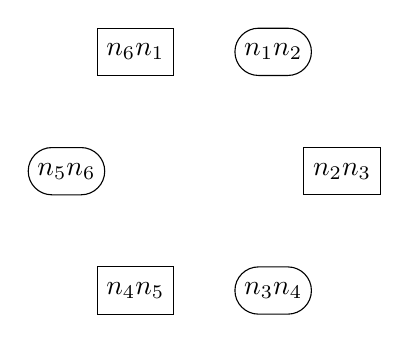
\begin{tikzpicture}[commutative diagrams/every diagram,
		one/.style={draw, rectangle, minimum size=6mm, rounded corners=3mm},
		two/.style={draw, rectangle, minimum size=6mm}
		]
		\node[one] (P0) at (60:1.75cm) {$n_1 n_2$};
		\node[two] (P1) at (60+60:1.75cm) {$n_6 n_1$} ;
		\node[one] (P2) at (60+2*60:1.75cm) {$n_5 n_6$};
		\node[two] (P3) at (60+3*60:1.75cm) {$n_4 n_5$};
		\node[one] (P4) at (60+4*60:1.75cm) {$n_3 n_4$};
		\node[two] (P5) at (0:1.75cm) {$n_2 n_3$};
	\end{tikzpicture}\end{center}

	三个 Herbrand 商对应到上图对角项的商. 断言 (i) 遂翻译为以下观察:
	\begin{itemize}
		\item 若某两条对角线两端的基数皆有限, 则剩下一条对角线两端亦然;
		\item 方框项乘积等于圆框项乘积.
	\end{itemize}
	
	至于 (ii), 存在有限 $\Z$-模的短正合列
	\[ 0 \to A^{\sigma=1} \to A \xrightarrow{\sigma-1} \mathfrak{I} A \to 0, \quad 0 \to A^{\nu=0} \to A \xrightarrow{\nu} \nu A \to 0; \]
	此处 $(\sigma - 1)A = \mathfrak{I}A$ 是引理 \ref{prop:cyclic-resolution-prep} 的应用. 于是
	\[ |A^{\sigma=1}| \cdot |\mathfrak{I} A| = |A^{\nu=0}| \cdot |\nu A|, \]
	此式又整理为 $|\TaHm^0(C_m, A)| = |\TaHm^{-1}(C_m, A)|$. 明所欲证.
\end{proof}

\section{pro-有限群的上同调}\label{sec:profinite-cohomology}
本节预设 \S\ref{sec:profinite-groups} 关于 pro-有限群的基本定义和结果.

设 $G$ 为 pro-有限群而 $M$ 为 $G$-模. 不难验证下述条件相互等价:
\begin{enumerate}[(i)]
	\item $M = \bigcup_K M^K$, 其中 $K$ 遍历 $G$ 的正规开子群;
	\item 对所有 $x \in M$, 稳定化子群 $\Stab_G(x)$ 是开的;
	\item 作用映射 $G \times M \to M$ 连续, 前提是赋 $M$ 离散拓扑.
\end{enumerate}

\begin{definition}
	\index{Gmo!光滑 (smooth)}
	\index[sym1]{G-Mod-infty@$G\dcate{Mod}^\infty$}
	设 $G$ 为 pro-有限群. 当以上任一条件成立时, 我们称 $G$-模 $M$ 是\emph{光滑}的\footnote{鉴于 (iii), 许多文献也称之为离散的.}. 全体光滑 $G$-模构成 $G\dcate{Mod}$ 的全子范畴 $G\dcate{Mod}^\infty$.
\end{definition}

虽然 $G$ 本身的条件涉及拓扑, 但光滑 $G$-模的刻画 (i) 或 (ii) 纯然是代数的, 它是 $G$-模的一种性质, 而非额外结构. 由此易见 $G\dcate{Mod}^\infty$ 是 $G\dcate{Mod}$ 的子 Abel 范畴. 定义 \ref{def:Res-Infl} 的操作在此有自然的类比.

\begin{definition-proposition}
	设 $\varphi: H \to G$ 为 pro-有限群之间的连续同态, $M$ 为光滑 $G$-模, 则 $H$-模 $\varphi^* M$ 仍光滑. 这给出函子
	\[ \varphi^*: G\dcate{Mod}^\infty \to H\dcate{Mod}^\infty. \]
\end{definition-proposition}
\begin{proof}
	对所有正规开子群 $K \lhd G$, 仍有相应的正规开子群 $\varphi^{-1}(K) \lhd H$. 若 $x \in M^K$, 则 $x \in (\varphi^* M)^{\varphi^{-1} K}$, 这说明 $\varphi^* M = \bigcup_{L \lhd H: \text{开}} (\varphi^* M)^L$. 故 $\varphi^* M$ 光滑.
\end{proof}

留意到函子 $\varphi^*$ 总是正合的. 在此拈出两类特例:
\begin{description}
	\item[限制] 设 $H$ 是 $G$ 的闭子群. 取 $\varphi$ 为包含同态 $H \hookrightarrow G$, 对应的函子记为
	\[ \Res^G_H: G\dcate{Mod}^\infty \to H\dcate{Mod}^\infty. \]
	\item[膨胀] 对于正规闭子群 $H \lhd G$, 取 $\varphi$ 为商同态 $G \twoheadrightarrow G/H$, 对应的函子记为
	\[ \mathrm{Infl}^G_{G/H}: G/H\dcate{Mod}^\infty \to G\dcate{Mod}^\infty. \]
	
	以上提及的群 $H$ 和 $G/H$ 自动是 pro-有限的, 故定义合理.
\end{description}
\index[sym1]{ResGH}
\index[sym1]{InflGH}

\begin{definition-proposition}\label{def:smooth-part}
	对任意 $G$-模 $M$, 定义 $M^\infty := \bigcup_K M^K$, 其中 $K$ 遍历 $G$ 的正规开子群. 这是光滑 $G$-模, 而 $M$ 光滑当且仅当 $M = M^\infty$.
	
	对于任意光滑 $G$-模 $M'$, 我们有
	\[ \Hom_G(M', M) = \Hom_G(M', M^\infty); \]
	换言之, $\text{包含}: G\dcate{Mod}^\infty \leftrightarrows G\dcate{Mod}: (\cdot)^\infty$ 是伴随对. 
\end{definition-proposition}
\begin{proof}
	显然.
\end{proof}

我们也称 $M^\infty$ 的元素为 $M$ 的\emph{光滑元素}. 既然 $(\cdot)^\infty$ 是正合函子的右伴随, 它保持内射对象 (命题 \ref{prop:adjoint-injective-projective}).

\begin{corollary}
	Abel 范畴 $G\dcate{Mod}^\infty$ 有足够的内射对象.
\end{corollary}
\begin{proof}
	设 $M$ 为光滑 $G$-模, 将它嵌入内射 $G$-模 $I$, 则 $M = M^\infty \hookrightarrow I^\infty$ 而 $I^\infty$ 是内射光滑 $G$-模.
\end{proof}

\begin{remark}
	一般而言 $G\dcate{Mod}^\infty$ 无足够的投射对象, 这是本节探讨上同调而非同调的主要原因.
\end{remark}

已知 $G\dcate{Mod}^\infty$ 有足够内射对象, 自然就可以谈论不变量函子 $(\cdot)^G$ 的右导出函子. 本节的进路是先表述化到有限群情形的直接定义, 随后在命题 \ref{prop:profinite-cohomology-identification} 将其等同于右导出函子. 以下仅用经典语言, 不论导出范畴.

首先考虑 pro-有限群 $G$ 及其正规开子群 $K$. 对任意光滑 $G$-模 $M$, 其中的 $K$-不变量 $M^K = (\Res^G_K M)^K$ 自然地成为 $G/K$-模, 由此得到函子 $(\cdot)^K: G\dcate{Mod}^\infty \to G/K\dcate{Mod}$. 我们有明白的伴随对
\begin{equation}\label{eqn:invariant-adjunction-profinite}
	\begin{tikzcd}[row sep=tiny]
		\mathrm{Infl}^G_{G/K}: G/K\dcate{Mod} \arrow[shift left, r] & G\dcate{Mod}^\infty : (\cdot)^K \arrow[shift left, l] \\
		\Hom_G\left(\mathrm{Infl}^G_{G/K}(M'), M\right) \arrow[equal, r] & \Hom_{G/K}\left( M', M^K \right).
	\end{tikzcd}
\end{equation}

若 $G$ 的正规开子群 $K$ 和 $K'$ 满足 $K' \supset K$, 则包含同态 $M^{K'} \hookrightarrow M^K$ 对反向的商同态 $G/K' \twoheadleftarrow G/K$ 等变 (定义 \ref{def:group-equivariance}), 于是对每个 $n \in \Z_{\geq 0}$ 都有典范同态
\[ \rho^{K'}_K: \Hm^n\left(G/K', M^{K'} \right) \to \Hm^n\left( G/K, M^K \right). \]

若 $K_1 \subset K_2 \subset K_3$ 是 $G$ 的正规开子群, 则 $\rho^{K_2}_{K_1} \rho^{K_3}_{K_2} = \rho^{K_3}_{K_1}$. 这表明以下定义合理.

\begin{definition}
	\index{quntongdiao!pro-有限情形}
	\index[sym1]{HnGM}
	设 $G$ 为 pro-有限群, $M$ 为光滑 $G$-模. 对所有 $n \in \Z_{\geq 0}$ 定义
	\[ \Hm^n(G, M) := \varinjlim_K \Hm^n\left(G/K, M^K \right), \quad n \in \Z_{\geq 0}, \]
	其中 $K$ 遍历 $G$ 的正规开子群, 而 $\varinjlim$ 按照 $K' \preceq K \iff K \subset K'$ 定义的偏序和 $\rho^{K'}_K$ 来定义.
\end{definition}

所有正规开子群构成滤过偏序集: 它们对有限交封闭. 若 $G$ 有限, 则 $\{1\}$ 是此偏序集的唯一极大元, 此时 $\Hm^n(G, M)$ 复归 \S\ref{sec:group-coh-sub} 的原始版本. 对于一般情形,
\[ \Hm^0(G, M) = \varinjlim_K \left(M^K\right)^{G/K} = M^G. \]

设 $f: M_1 \to M_2$ 为光滑 $G$-模之间的同态. 对所有正规开子群 $K$, 它限制为 $f_K: M_1^K \to M_2^K$. 显然 $K' \supset K$ 蕴涵 $\Hm^n(f_K) \rho^{K'}_K = \rho^{K'}_K \Hm^n(f_{K'})$, 对所有 $n \in \Z_{\geq 0}$ 遂有
\[ \Hm^n(f): \Hm^n(G, M_1) \to \Hm^n(G, M_2) \]

\begin{example}
	设 $E|F$ 为域的 Galois 扩张. 由于 $E = \bigcup_{L|F} E^{\Gal(E|L)} = \bigcup_{L|F} L$, 其中 $L|F$ 遍历有限 Galois 子扩张, 故 $\Gal(E|F)$ 对 $E$ 的作用光滑. 对每个 $L|F$ 运用例 \ref{eg:additive-90-finite} 可得
	\[ n \geq 1 \implies \Hm^n(\Gal(E|F), E) = \varinjlim_{L|F} \Hm^n(\Gal(L|F), L) = 0. \]
\end{example}

一如 $G$ 不带拓扑时的命题 \ref{prop:groupcoh-cochain} 和注记 \ref{rem:nor-cochain}, pro-有限群的上同调也可以由标准复形或其正规化版本来计算, 差异在于连续性条件.

\begin{definition}
	\index{biaozhunfuxing}
	\index[sym1]{CGM}
	对任意光滑 $G$-模 $M$, 赋予 $M$ 离散拓扑并定义其\emph{标准复形} $C(G, M) = (C^n(G, M))_n$ 如下:
	\begin{gather*}
		C^n(G, M) := \left\{ \text{连续映射}\; f: G^n \to M \right\}, \quad n \in \Z_{\geq 0},
	\end{gather*}
	负次项定义为 $0$, 而 $d^n: C^n(G, M) \to C^{n+1}(G, M)$ 定义为
	\begin{multline*}
		(d^n f)(g_1, \ldots, g_{n+1}) = g_1 f(g_2, \ldots, g_{n+1}) \\
		+ \sum_{k=1}^n (-1)^k f(\ldots, g_k g_{k+1}, \ldots) + (-1)^{n+1} f(g_1, \ldots, g_n).
	\end{multline*}

	\index[sym1]{CGMbar}
	定义\emph{正规化标准复形}为 $C(G, M)$ 的子复形 $\overline{C}(G, M)$ 如下 (见注记 \ref{rem:nor-cochain})
	\[ \overline{C}^n(G, M) = \left\{\begin{array}{r|l}
		f \in C^n(G, M) & \exists 1 \leq k \leq n, \; g_k = 1_G \\
		& \implies f(g_1, \ldots, g_n) = 0
	\end{array}\right\}. \]
\end{definition}

对于所有正规开子群 $K \lhd G$, 我们有复形之间的自明嵌入 $C(G/K, M^K) \hookrightarrow C(G, M)$ 和 $\overline{C}(G/K, M^K) \hookrightarrow \overline{C}(G, M)$.

由于 $M$ 离散, 映射 $f: G^n \to M$ 连续相当于说它是局部常值映射, 故由 $G$ 紧可得正规开子群 $K_1 \lhd G$ 使得 $f$ 分解为 $(G/K_1)^n \to M$; 特别地, $f$ 取有限多个值, 故光滑性导致存在正规开子群 $K_2 \lhd G$ 使得 $f$ 取值在 $M^{K_2}$. 命 $K := K_1 \cap K_2$, 综上可知,
\[ C^n(G, M) \simeq \varinjlim_{K \lhd G\; \text{开}} C^n\left(G/K, M^K\right), \quad \overline{C}^n(G, M) \simeq \varinjlim_{K \lhd G\; \text{开}} \overline{C}^n\left(G/K, M^K\right), \]
当 $n$ 变动, 这给出复形之间的同构.

依照往例, 定义 $C^n(G, M)$ 的子模
\[ Z^n(G, M) := \Ker(d^n), \quad B^n(G, M) := \Image(d^{n-1}), \]
此处规定 $B^0(G, M) := \{0\}$. 于是 $\Hm^n(C(G, M)) = Z^n(G, M) / B^n(G, M)$. 以类似手法定义正规化版本 $\overline{Z}^n(G, M)$ 和 $\overline{B}^n(G, M)$.

\begin{theorem}\label{prop:profinite-group-standard}
	设 $G$ 为 pro-有限群. 对所有 $n \in \Z_{\geq 0}$ 和光滑 $G$-模, 存在典范同构 $\Hm^n(C(G, M)) \simeq \Hm^n(G, M) \simeq \Hm^n(\overline{C}(G, M))$.
\end{theorem}
\begin{proof}
	上同调取值在 $\cate{Ab}$ 或 $\Bbbk\dcate{Mod}$ (若另选系数环 $\Bbbk$); 滤过 $\varinjlim$ 在这些范畴中是正合的 \cite[定理 6.2.2]{Li1}, 故
	\[ Z^n(G, M) = \varinjlim_K Z^n(G/K, M^K), \quad B^n(G, M) = \varinjlim_K B^n(G/K, M^K), \]
	继而
	\begin{multline*}
		\Hm^n(C(G, M)) = \dfrac{\varinjlim_K Z^n(G/K, M^K)}{\varinjlim_K B^n(G/K, M^K)} \simeq \\
		\varinjlim_K \frac{Z^n(G/K, M^K)}{B^n(G/K, M^K)} = \varinjlim_K \Hm^n(C(G/K, M^K)).
	\end{multline*}
	对末项应用命题 \ref{prop:groupcoh-cochain} 以得到 $\varinjlim_K \Hm^n(G/K, M^K)$, 即 $\Hm^n(G, K)$.
	
	关于 $\overline{C}(G, M)$ 的情形是类似的.
\end{proof}

\begin{theorem}\label{prop:profinite-cohomology-long}
	设 $G$ 为 pro-有限群. 设 $0 \to M' \xrightarrow{f} M \xrightarrow{f'} M'' \to 0$ 是光滑 $G$-模的短正合列, 则有相应的长正合列
	\begin{multline*}
		\cdots \to \Hm^{n-1}(G, M'') \xrightarrow{\delta^{n-1}} \Hm^n(G, M') \xrightarrow{\Hm^n(f)} \Hm^n(G, M) \\
		\xrightarrow{\Hm^n(g)} \Hm^n(G, M'') \xrightarrow{\delta^n} \Hm^{n+1}(G, M') \to \cdots ,
	\end{multline*}
	其中规定 $n <0 $ 时 $\Hm^n(G, \cdot) = 0$. 连接同态 $\delta^n$ 对短正合列之间的态射具有函子性; 换言之, 它们给出上同调 $\delta$-函子.
\end{theorem}
\begin{proof}
	我们将在标准复形上操作; 正规化版本的论证是类似的. 鉴于熟知的命题 \ref{prop:long-exact-sequence-ses}, 要点归结为说明
	\[ 0 \to C^n(G, M') \to C^n(G, M) \to C^n(G, M'') \to 0 \]
	是短正合列. 唯一相对不平凡的是 $C^n(G, M) \to C^n(G, M'')$ 的满性: 设 $f: G^n \to M''$ 为连续映射, 如前所见, 存在正规开子群 $K \lhd G$ 使得 $f$ 在 $K^n \lhd G^n$ 的每个陪集上都取常值, 然后在每个陪集上任意指定此常值在 $M$ 中的原像即可.
\end{proof}

取光滑 $G$-模 $M$, 赋予离散拓扑. 复形 $C(G, M)$ 或 $\overline{C}(G, M)$ 的低次项仍然有直接的诠释.
\begin{description}
	\item[($n=0$)] 显然 $C^0(G, M) = M$ 而 $\Hm^0(G, M) = Z^0(G, M) = M^G$. 正规化标准复形的版本无异.
	\item[($n=1$)] $Z^1(G, M) = \overline{Z}^1(G, M)$ 的元素是连续叉同态 $G \to M$, 等价地说则是满足 $\pi \sigma = \identity_G$ 的连续同态 $\sigma: G \to M \rtimes G$, 如命题 \ref{prop:crossed-semidirect-product}; 在此 $\pi: M \rtimes G \to G$ 是投影, 而 $M \rtimes G$ 带乘积拓扑. 另一方面, $B^1(G, M)$ 的元素由形如 $f_m: g \mapsto gm - m$ 的叉同态生成, 它们自动连续.
	
	\item[($n=2$)] 设 $M$ 有限, 则 $\Hm^2(G, M) \simeq \frac{Z^2(G, M)}{B^2(G, M)} \simeq \frac{\overline{Z}^2(G, M)}{\overline{B}^2(G, M)}$ 的元素一一对应于 pro-有限群扩张
	\[ 0 \to M \to E \xrightarrow{\pi} G \to 0 \quad \text{(群的短正合列)} \]
	的等价类, 要求 $G$ 对 $M$ 的共轭作用来自 $M$ 的 $G$-模结构; 相较于定义 \ref{def:group-ext} 和 \eqref{eqn:group-ext-diagram} 的版本, 所谓的 ``pro-有限群扩张''及其分类问题进一步要求:
	\begin{compactitem}
		\item $E$ 是 pro-有限群, $\pi$ 连续, 而 $M$ 嵌入为 $E$ 的闭子群;
		\item 扩张的等价或曰同构由连续的群同态 $E \to E'$ 定义, 扩张的分裂同样以拓扑方式定义.
	\end{compactitem}

	此外, 扩张的自同构群同构于 $\overline{Z}^1(G, M)$. 这些证明并不难, 但是需要一些拓扑语言, 故留作本章习题; $M$ 有限的条件是关键的.
\end{description}

现在回头探讨 $(\cdot)^G$ 的右导出函子 $\left(\mathrm{R}^n (\cdot)^G\right)_{n \geq 0}$. 尽管可以探讨它在任意下有界复形上的取值 \footnote{换言之, 探讨 pro-有限群的超上同调.}, 乃至于导出范畴中的操作等, 但本节只论光滑 $G$-模的情形, 其余划入习题.

\begin{proposition}\label{prop:profinite-cohomology-identification}
	我们有上同调 $\delta$-函子的同构 $\left( \Hm^n(G, \cdot) \right)_{n \geq 0} \simeq \left(\mathrm{R}^n (\cdot)^G\right)_{n \geq 0}$.
\end{proposition}
\begin{proof}
	定理 \ref{prop:profinite-cohomology-long} 说明两者都是上同调 $\delta$-函子, 而且在 $n=0$ 时同样化为不变量函子 $(\cdot)^G$. 鉴于命题 \ref{prop:erasable-univ-delta}, 问题归结为说明当 $n > 0$ 时 $\Hm^n(G, \cdot)$ 是定义 \ref{def:erasable} 所谓的可拭函子. 设 $M$ 为光滑 $G$-模, 将其嵌入内射光滑 $G$-模 $I$. 对于所有正规开子群 $K \lhd G$, 伴随关系 \eqref{eqn:invariant-adjunction-profinite} 蕴涵 $(\cdot)^K$ 保持内射对象, 故 $I^K$ 是内射 $G/K$-模. 因此
	\[ n > 0 \implies \Hm^n(G, I) = \varinjlim_K \Hm^n\left( G/K, I^K\right) = 0. \]
	可拭性质得证.
\end{proof}

基于命题 \ref{prop:profinite-cohomology-identification}, 照搬 \S\ref{sec:change-of-group} 的方法即可对 pro-有限群的连续同态 $\varphi: H \to G$ 定义上同调的``拉回''运算
\[ \Hm^n(G, M) \to \Hm^n(H, \varphi^* M), \quad M: \text{光滑 $G$-模}, \; n \in \Z_{\geq 0}, \]
它们兼容长正合列. 一如既往地, 方法是运用 $\varphi^*$ 的正合性以及泛上同调 $\delta$-函子的性质, 将问题归结为 $n=0$ 情形的自明嵌入 $M^G \hookrightarrow (\varphi^* M)^H$.

作为特例, 对所有 $n$ 和闭子群 $H$ 都有限制映射 $\mathrm{res}^n: \Hm^n(G, M) \to \Hm^n(H, M)$, 此处将 $\Res^G_H M$ 简记为 $M$.

上述同态也可以构造为诸
\begin{align*}
	\Hm^n\left( G/K, M^K\right) & \xrightarrow{\eqref{eqn:change-of-group-coh}} \Hm^n\left(H/\varphi^{-1}(K), \; \varphi_K^*(M^K)\right) \\
	& \xrightarrow{M^K \subset (\varphi^* M)^{\varphi^{-1} K}} \Hm^n\left( H/\varphi^{-1}(K), \; (\varphi^* M)^{\varphi^{-1} K}\right)
\end{align*}
确定的 $\Hm^n(G, M) \to \Hm^n(H, \varphi^* M)$, 其中 $K$ 遍历 $G$ 的正规开子群. 化约到有限群情形可见此同态在标准复形上由命题 \ref{prop:grp-equiv} 的公式计算. 为了说明它确实等于之前按照泛性质构造的同态, 仅须比较 $n=0$ 情形, 并说明同态兼容长正合列即可. 标准复形足以处理这些问题.

类似地, 定义--命题 \ref{def:cor} 的余限制同态也扩展到 pro-有限群情形. 设 $H$ 为 $G$ 的开子群, 此时它自动闭, 而且 $(G: H)$ 有限 (见 \S\ref{sec:profinite-groups}). 今将定义同态
\[ \mathrm{cor}^n: \Hm^n(H, M) \to \Hm^n(G, M), \quad M: \text{光滑 $G$-模}, \; n \in \Z_{\geq 0}, \]
使得它们兼容长正合列, 并且在 $n=0$ 时给出 $\nu^{G|H}: M^H \to M^G$.

构造依旧基于泛上同调 $\delta$-函子的性质, 但此处需要知道 $\Res^G_H: G\dcate{Mod}^\infty \to H\dcate{Mod}^\infty$ 保持内射对象, 这是稍后的推论 \ref{prop:Res-injective-profinite} 的内容. 一旦承认这点, 则命题 \ref{prop:res-cor} 仍然有类比: 对所有 $n$ 皆有
\[ \mathrm{cor}^n \circ \mathrm{res}^n = (G:H) \cdot \identity_{\Hm^n(G, M)}. \]
方法照旧, 化约到 $n=0$ 来验证.

现在来探讨 pro-有限情形的诱导模. 默认 $G$ 为 pro-有限群. 为了区别, 记不带拓扑情形的诱导函子 (定义 \ref{def:induced-module}) 为 $\Ind^{G, \mathrm{alg}}_H$ 以资区分; 我们按照引理 \ref{prop:Ind-as-mappings} 将其实现为一个映射空间.

\begin{definition}
	\index{Gmo!诱导 (induced)}
	对于 $G$ 的闭子群 $H$ 连同光滑 $H$-模 $N$, 赋予映射空间 $\mathrm{Maps}(G, N) := \{f: G \to N \}$ 逐点的加法和纯量乘法运算, 连同以下的左 $G$-作用
	\[ (gf)(x) = f(xg), \quad g, x \in G. \]
	由此定义光滑 $G$-模
	\begin{align*}
		\Ind^G_H(N) & := \left\{ f \in \mathrm{Maps}(G, N)^\infty : \forall h \in H, \; \forall x \in G, \; f(hx) = hf(x) \right\} \\
		& = \left( \Ind^{G, \mathrm{alg}}_H(N)\right)^\infty
	\end{align*}
	符号 $(\cdot)^\infty$ 见定义--命题 \ref{def:smooth-part}. 这称为 $N$ 的诱导 $G$-模.
\end{definition}

因为 $G$ 紧, $f \in \Ind^{G, \mathrm{alg}}_H(N)$ 的光滑性等价于它作为映射 $G \to N$ 的连续性, 前提是赋予 $N$ 离散拓扑.

\begin{proposition}\label{prop:Ind-injective-profinite}
	对于 $G$ 的所有闭子群 $H$ 都有伴随对
	\[ \Res^G_H: G\dcate{Mod}^\infty \leftrightarrows H\dcate{Mod}^\infty : \Ind^G_H; \]
	作为推论, $\Ind^G_H$ 保持内射对象.
	
	若 $H$ 是 $G$ 的开子群, 则还有伴随对
	\[ \Ind^G_H : H\dcate{Mod}^\infty \leftrightarrows G\dcate{Mod}^\infty : \Res^G_H ; \]
	此时 $\Ind^G_H$ 也保持投射对象.
\end{proposition}
\begin{proof}
	基于无拓扑情形的伴随关系和定义--命题 \ref{def:smooth-part}, 对所有光滑 $G$-模 $M$ 和光滑 $H$-模 $N$ 皆有典范同构
	\begin{multline*}
		\Hom_H\left( \Res^G_H(M), N \right) \simeq \Hom_G\left(M, \Ind^{G, \mathrm{alg}}_H(N) \right) \\
		= \Hom_G\left(M, \Ind^{G, \mathrm{alg}}_H(N)^\infty \right) = \Hom_G\left(M, \Ind^G_H(N) \right).
	\end{multline*}
	
	现在假设 $H$ 是开子群, 于是 $(G:H)$ 有限. 我们从推论 \ref{prop:iInd-Ind} 得到无拓扑情形的伴随关系
	\[ \Hom_H\left(N, \Res^G_H(M)\right) \simeq \Hom_G\left( \Ind^{G, \mathrm{alg}}_H(N) , M\right). \]
	兹断言 $\Ind^{G, \mathrm{alg}}_H(N) = \Ind^G_H(N)$. 给定 $f \in \Ind^{G, \mathrm{alg}}_H(N)$ 和 $x \in G$, 取 $H$ 的开子群 $K_0$ 使得 $f(x) \in N^{K_0}$; 命 $K := x^{-1} K_0 x$, 这是 $G$ 的开子群, 于是有
	\[ g \in K \implies xg = xgx^{-1} x \in K_0 x \implies f(xg) = f(x). \]
	既然 $x$ 任意, 这说明 $f: G \to N$ 是局部常值映射, 故 $f \in \Ind^G_H(N)$. 第二个伴随对得证.
	
	最后, 关于保持内射或投射对象的断言不外是 $\Res^G_H$ 的正合性连同命题 \ref{prop:adjoint-injective-projective} 的应用.
\end{proof}

\begin{lemma}\label{prop:Ind-exact-profinite}
	设 $H$ 是 $G$ 的闭子群, 则 $\Ind^G_H: H\dcate{Mod}^\infty \to G\dcate{Mod}^\infty$ 是正合函子.
\end{lemma}
\begin{proof}
	已知 $\Ind^G_H$ 有左伴随, 故左正合. 问题归结为证明 $N_1 \twoheadrightarrow N_2 \implies \Ind^G_H(N_1) \twoheadrightarrow \Ind^G_H(N_2)$. 以引理 \ref{prop:profinite-section} 取商同态 $\pi: G \to H \backslash G$ 的连续截面 $s$, 于是对所有光滑 $H$-模 $N$ 皆有 $\Bbbk$-模同构
	\[\begin{tikzcd}[row sep=tiny]
		\Ind^G_H(N) \arrow[leftrightarrow, r, "\sim"] & \left\{\text{连续映射}\; H\backslash G \to N \right\} \\
		f \arrow[mapsto, r] & {[x \mapsto f(s(x)) ]} \\
		{[h s(x) \mapsto hf'(x) ]} & f' , \arrow[mapsto, l]
	\end{tikzcd}\]
	其中 $x \in H \backslash G$ 而 $h \in H$. 虽然同构不保持 $G$-作用, 但它对 $N$ 具有函子性.
	
	由于连续映射 $H \backslash G \to N$ 总是局部常值的, 在上式右侧操作, 便不难说明映射 $\Ind^G_H(N_1) \to \Ind^G_H(N_2)$ 为满.
\end{proof}

\begin{corollary}\label{prop:Res-injective-profinite}
	设 $H$ 是 $G$ 的开子群, 则 $\Res^G_H: G\dcate{Mod}^\infty \to H\dcate{Mod}^\infty$ 保持内射对象.
\end{corollary}
\begin{proof}
	基于前两则结果, 它有正合的左伴随 $\Ind^G_H$.
\end{proof}

现在得到定理 \ref{prop:Shapiro} 的 pro-有限群版本.

\begin{proposition}
	\index{Shapiro yinli}
	设 $H$ 为 pro-有限群 $G$ 的闭子群, $N$ 为 $H$-模. 我们有同构
	\[ \Hm^n\left(G, \Ind^G_H(N)\right) \simeq \Hm^n(H, N), \quad n \in \Z_{\geq 0}. \]
\end{proposition}
\begin{proof}
	基于 $\Ind^G_H$ 正合而且保持内射对象这一事实 (引理 \ref{prop:Ind-exact-profinite}), 定理 \ref{prop:Shapiro} 中涉及可拭上同调 $\delta$-函子的论证全盘照搬. 回忆到该处论证的关键是 $n=0$ 情形, 相当于
	\[ \Ind^G_H(N)^G = \left(\Ind^{G, \mathrm{alg}}_H(N)^\infty \right)^G = \left(\Ind^{G, \mathrm{alg}}_H(N)\right)^G \rightiso N^H; \]
	第一个等号是定义, 第二个等号是容易的, 而末段同构来自推论 \ref{prop:Ind-invariant}.
\end{proof}

除此之外,
\begin{itemize}
	\item 上同调的 Lyndon--Hochschild--Serre 谱序列 (见 \S\ref{sec:LHS-SS}) 可以推广到 $G$ 为 pro-有限群而 $H$ 为正规闭子群的情形;
	\item 杯积 (见 \S\ref{sec:cup-product}) 也可以推广到 pro-有限群, 方法是采用标准复形上的直接定义, 参看定义--命题 \ref{def:group-cup-3}.
	\index{beiji}
\end{itemize}
表述无异, 不再赘述.

\section{非交换上同调}\label{sec:nonabelian-coh}
设 $G$ 为群. 先前讨论的上同调 $\Hm^n(G, M)$ 总要求其``系数'' $M$ 具有模结构, 或者至少是 $\Z$-模, 亦即交换群. 本节旨在探讨系数为非交换群的情形. 今起改用符号 $A$ 代替 $M$.

\begin{definition}\label{def:G-group}
	\index[sym1]{G-Grp@$G\dcate{Grp}$}
	\index{G-qun@$G$-群}
	设 $A$ 为群, 二元运算写作乘法, 幺元记为 $1$. 如果 $A$ 带有群 $G$ 的左作用, 写作
	\[ G \times A \to A, \quad (g, a) \mapsto {}^g a . \]
	使得群作用兼容 $A$ 的乘法结构:
	\[ {}^g (a_1 a_2) = {}^g a_1 {}^g a_2, \quad {}^g 1 = 1, \]
	则称 $A$ 是带 $G$-作用的群, 简称 $G$-群. 定义 $G$-群之间的同态为保持 $G$-作用的群同态. 它们构成的范畴记为 $G\dcate{Grp}$.
\end{definition}

即将看到, 对于 $G$-群 $A$, 在缺少额外结构或交换性的前提下, 能合理而且实用地定义的只有 $\Hm^0$ 和 $\Hm^1$. 此时 $\Hm^1$ 未必是群, 而是带基点集.

\begin{definition}\label{def:pointed-set}
	\index{daijidianji@带基点集 (pointed set)}
	\index[sym1]{Set-pt@$\cate{Set}_\bullet$, $G\dcate{Set}_\bullet$}
	所谓带基点集, 意谓资料 $(X, x_0)$, 其中 $X$ 是集合而 $x_0 \in X$ (称为基点); 从 $(X, x_0)$ 到 $(Y, y_0)$ 的态射意谓满足 $f(x_0) = y_0$ 的映射 $f: X \to Y$. 这些资料构成范畴 $\cate{Set}_\bullet$.
	
	设 $(X, x_0)$ 是带基点集. 若群 $G$ 左作用在 $X$ 上, 写作 $(g, x) \mapsto {}^g x$, 而且 ${}^g x_0 = x_0$ 恒成立, 则称 $G$ 作用在 $(X, x_0)$ 上. 此时可定义带基点的不变量子集
	\[ (X, x_0)^G := \left\{ x \in X: \forall g \in G, \; gx = x \right\}, \quad \text{基点} = x_0. \]
	全体具有 $G$-作用的带基点集对兼容于 $G$-作用的态射构成范畴, 记为 $G\dcate{Set}_\bullet$.
\end{definition}

不致混淆时, 我们经常将 $\cate{Set}_\bullet$ 的对象 $(X, x_0)$ 记为 $X$, 在 $G\dcate{Set}_\bullet$ 的场合将 $(X, x_0)^G$ 记为 $X^G$.

群当然地成为带基点集, 基点取为群的幺元, 这给出不言自明的函子 $\cate{Grp} \to \cate{Set}_\bullet$; 同理也有 $G\dcate{Grp} \to G\dcate{Set}_\bullet$. 请留意到 $G$-群 $A$ 的不变量子集 $A^G$ 是其子群.

\begin{definition}\label{def:pointed-exact}
	\index{zhenghelie}
	设 $(X, x_0) \xrightarrow{f} (Y, y_0) \xrightarrow{g} (Z, z_0)$ 为 $\cate{Set}_\bullet$ (或 $G\dcate{Set}_\bullet$) 中的态射. 若 $g^{-1}(z_0) = \Image(f)$, 则称此列态射正合. 由之可在 $\cate{Set}_\bullet$ (或 $G\dcate{Set}_\bullet$) 中定义何谓正合列.
\end{definition}

这在交换群的情形回归熟知的正合性. 现在可以对任意 $G$-群 $A$ 陈述 $\Hm^0$ 和 $\Hm^1$ 的定义.

\begin{definition}\label{def:nonabelian-H}
	\index{quntongdiao!非交换情形}
	设 $A$ 为 $G\dcate{Set}_\bullet$ 的对象. 定义带基点集
	\[ \Hm^0(G, A) = Z^0(G, A) := A^G. \]
	
	当 $A$ 是 $G$-群时 $\Hm^0(G, A)$ 成群. 此时进一步定义
	\begin{align*}
		Z^1(G, A) & := \left\{\begin{array}{r|l}
			c: G \to A & \forall g_1, g_2 \in G, \\
			& c(g_1 g_2) = c(g_1) \cdot {}^{g_1} c(g_2)
		\end{array}\right\}, \\
		\Hm^1(G, A) & := Z^1(G, A) / \sim ,
	\end{align*}
	等价关系 $c \sim c'$ 意谓存在 $a \in A$ 使得对所有 $g \in G$ 皆有
	\[ c'(g) = a^{-1} \cdot c(g) \cdot {}^g a . \]
	易见这确实为等价关系 (它来自某个右 $A$-作用), 而 $\Hm^1(G, A)$ 自然地成为带基点集, 以常值映射 $c(g) = 1$ 决定的等价类为其基点.
\end{definition}

留意到在 $Z^1(G, A)$ 的条件中代入 $g_1 = g_2 = 1_G$ 可得 $c(1_G) = 1$. 今后以 $[c]$ 代表 $c \in Z^1(G, A)$ 的等价类.

\begin{remark}[$\Hm^1$ 作为截面的共轭类]\label{rem:Z1-vs-section}
	从 $G$-群 $A$ 构造半直积 $A \rtimes G$, 记投影同态 $A \rtimes G \to G$ 为 $\pi$, 则, $Z^1(G, A)$ 的元素一一对应于满足 $\pi \sigma = \identity_G$ 的群同态 $\sigma: G \to A \rtimes G$ (亦即 $\pi$ 的``截面''), 方法是映 $c \in Z^1(G, A)$ 为 $\sigma(g) = (c(g), g)$. 进一步, $[c'] = [c]$ 等价于存在 $a \in A$ 使得 $\sigma' = a^{-1} \sigma a$, 其中 $A$ 嵌入为 $A \rtimes G$ 的子群, 逐点作共轭.
\end{remark}

当 $A$ 是交换群时, 这些构造化为基于标准复形对 $\Hm^0$ 和 $\Hm^1$ 作出的描述 (命题 \ref{prop:groupcoh-cochain}). 它们在非交换情形依然具有函子性, 细说如下.
\begin{itemize}
	\item 任何态射 $f: A_1 \to A_2$ 都诱导
	\begin{gather*}
		\Hm^0(f): \Hm^0(G, A_1) \to \Hm^0(G, A_2), \quad
		\Hm^1(f): \Hm^1(G, A_1) \to \Hm^1(G, A_2);
	\end{gather*}
	前者显然, 后者的映法则是 $\Hm^1(f)([c]) = [f \circ c]$.
	
	\item 设 $\varphi: H \to G$ 为群同态. 将 $G$-群 $A$ 的 $G$-作用拉回到 $H$ 上, 给出 $H$-群 $\varphi^* A$.
	\begin{compactitem}
		\item 定义典范态射 $\Hm^0(G, A) \to \Hm^0(H, \varphi^* A)$ 	为自明嵌入 $A^G \hookrightarrow A^{\varphi(H)} = (\varphi^* A)^H$.
		\item 以 $[c] \mapsto [c \circ \varphi]$ 定义带基点集的典范态射
		\[ \Hm^1(G, A) \to \Hm^1(H, \varphi^* A). \]
	\end{compactitem}
\end{itemize}

这些典范映射具有如 \S\ref{sec:change-of-group} 所见的诸般性质. 它们还可以统合如下: 给定 $\varphi: H \to G$, 设 $A_1$ 是 $G\dcate{Set}_\bullet$ (或 $G\dcate{Grp}$) 的对象, $A_2$ 是 $H\dcate{Set}_\bullet$ (或 $H\dcate{Grp}$) 的对象, 而态射 $f: A_1 \to A_2$ 对 $\varphi$ 等变 (一如定义 \ref{def:group-equivariance}), 则有相应的 $\Hm^i(f): \Hm^i(G, A_1) \to \Hm^i(H, A_2)$, 使得命题 \ref{prop:grp-equiv} 有如下类比:
\begin{itemize}
	\item $\Hm^0(f)$ 是 $f$ 限制而成的 $A_1^G \to A_2^H$,
	\item $\Hm^1(f)$ 映 $[c]$ 为 $[f \circ c \circ \varphi]$.
\end{itemize}

\begin{convention}
	记独点集在 $\cate{Set}_\bullet$ 或 $G\dcate{Set}_\bullet$ 中确定的零对象为 $1$.
\end{convention}

进入正题. 今起考虑 $G\dcate{Set}_\bullet$ 中的短正合列 (定义 \ref{def:pointed-exact})
\[ 1 \to A \xrightarrow{u} B \xrightarrow{v} C \to 1, \]
其中默认 $A$ 和 $B$ 是 $G$-群, $u$ 是群同态, 故正合性蕴涵 $u$ 单 $v$ 满; 我们进一步要求:
\begin{equation}\label{eqn:pointed-ses-condition}
	\begin{gathered}
		\forall b, b' \in B, \; \left[ v(b) = v(b') \iff \exists a \in A, \; b' = b u(a) \right], \\
		\text{换言之: $C$ 等同于 $B/u(A)$, 基点 $= 1 \cdot u(A)$.}
	\end{gathered}
\end{equation}

假若 $C$ 是群而 $v$ 是群同态, 则考虑 $b^{-1} b' \in v^{-1}(1) = \Image(u)$ 可知 \eqref{eqn:pointed-ses-condition} 自动成立, 而且此时 $u(A) \lhd B$; 然而许多应用场景并非如此.

眼下目标是为这些资料建立一个``尽可能长''正合列和对应的连接态射. 我们将不加说明地将 $A$ 等同于 $B$ 的子群, 同时省略符号 $u$.

\textbf{零次情形.}\;
首先定义连接态射 $\delta^0: \Hm^0(G, C) \to \Hm^1(G, A)$. 设 $c \in C^G$. 任取 $b \in v^{-1}(c)$. 因为 $v$ 保持 $G$-作用, 由 \eqref{eqn:pointed-ses-condition} 可知对所有 $g \in G$ 皆存在唯一的 $a(g) \in A$ 使得 ${}^g b = ba(g)$. 于是 $g \mapsto a(g)$ 给出 $Z^1(G, A)$ 的元素 $a$, 这是因为
\[ a(g_1 g_2) = b^{-1} \cdot {}^{g_1 g_2} b = b^{-1} \cdot {}^{g_1} b \cdot {}^{g_1} (b^{-1} \cdot {}^{g_2} b) = a(g) \cdot {}^{g_1} a(g_2). \]
若 $b', b \in v^{-1}(c)$, 则存在 $\alpha \in A$ 使得 $b' = b\alpha$, 于是
\[ (b')^{-1} \cdot {}^g b' = \alpha^{-1} \cdot b^{-1} \cdot {}^g b \cdot {}^g \alpha. \]
这说明类 $[a] \in \Hm^1(G, A)$ 仅由 $c$ 确定. 如果 $c$ 是 $C$ 的基点, 则可取 $b = 1 \in B$. 综上可得 $\cate{Set}_\bullet$ 中的态射 $\delta^0: \Hm^0(G, C) \to \Hm^1(G, A)$.

\textbf{零次情形: 中心子群.}\;
假定 $C$ 是群, $v$ 是群同态, 而 $A$ 包含于群 $B$ 的中心 $Z_B$; 特别地, $A$ 是交换群. 此时 $\Hm^0(G, C) = C^G$ 和 $\Hm^1(G, A)$ 都是群. 根据 $\delta^0$ 的定义和条件 $A \subset Z_B$, 容易验证 $\delta^0$ 是群同态.

\textbf{一次情形.}\;
继续假定 $C$ 是群而 $v$ 是群同态, $A \subset Z_B$; 于是 $\Hm^2(G, A)$ 可由标准复形描述. 今将定义 $\delta^1: \Hm^1(G, C) \to \Hm^2(G, A)$. 设 $c \in Z^1(G, C)$. 对每个 $g \in G$ 选取 $b(g) \in v^{-1}(c(g))$. 由于 \eqref{eqn:pointed-ses-condition} 总成立, 而 $v$ 保持 $G$-作用, 存在唯一的映射 $a: G^2 \to A$ 使得
\[ b(g_1) \cdot {}^{g_1} b(g_2) = a(g_1, g_2) b(g_1 g_2). \]

现在验证 $a \in Z^2(G, A)$. 这等价于
\[ a(g_1, g_2)^{-1} \cdot a(g_1, g_2 g_3) \cdot a(g_1 g_2, g_3)^{-1} \cdot {}^{g_1} a(g_2, g_3) = 1. \]
将左式展开成 $B$ 中的表达式
\begin{multline*}
	\underbracket{b(g_1 g_2) \cdot {}^{g_1} b(g_2)^{-1} \cdot b(g_1)^{-1}}_{a(g_1, g_2)^{-1}} \cdot \underbracket{b(g_1) \cdot {}^{g_1} b(g_2 g_3) b(g_1 g_2 g_3)^{-1}}_{a(g_1, g_2 g_3)} \\
	\underbracket{b(g_1 g_2 g_3) \cdot {}^{g_1 g_2} b(g_3)^{-1} \cdot b(g_1 g_2)^{-1}}_{a(g_1 g_2, g_3)^{-1}} \; \cdot \; {}^{g_1} a(g_2, g_3),
\end{multline*}
再用 $A \subset Z_B$ 化简为
\begin{multline*}
	b(g_1 g_2) \cdot {}^{g_1} b(g_2)^{-1} \cdot {}^{g_1} b(g_2 g_3) \cdot {}^{g_1 g_2} b(g_3)^{-1}  b(g_1 g_2)^{-1} \cdot {}^{g_1} a(g_2, g_3) \\
	= b(g_1 g_2) \cdot {}^{g_1} b(g_2)^{-1} \cdot \underbracket{{}^{g_1} b(g_2) \cdot {}^{g_1 g_2} b(g_3) \cdot {}^{g_1} b(g_2 g_3)^{-1}}_{{}^{g_1} a(g_2, g_3)} \cdot {}^{g_1} b(g_2 g_3) \cdot {}^{g_1 g_2} b(g_3)^{-1}  b(g_1 g_2)^{-1} .
\end{multline*}
至此可见末式确实等于 $1$, 故 $a \in Z^2(G, A)$.

若改变各个 $b(g)$ 的选取, 表作 $b'(g) = \alpha(g) b(g)$, 其中 $\alpha: G \to A$ 是任意映射, 则对应之 $a'(g_1, g_2)$ 等于
\begin{align*}
	a'(g_1, g_2) & = \alpha(g_1) \cdot b(g_1) \cdot {}^{g_1} \alpha(g_2) \cdot {}^{g_1} b(g_2) b(g_1 g_2)^{-1} \alpha(g_1 g_2)^{-1} \\
	& = \alpha(g_1) \cdot {}^{g_1} \alpha(g_2) \cdot \alpha(g_1 g_2)^{-1} \cdot a(g_1, g_2) \quad (\because\; A \subset Z_B).
\end{align*}
于是 $a, a' \in Z^2(G, A)$ 仅差一个 $B^2(G, A)$ 的元素.

最后考虑 $c$ 被代换为 $c'(g) = \gamma^{-1} \cdot c(g) \cdot {}^g \gamma$ 的情形, $\gamma \in C$. 任取 $\beta \in v^{-1}(\gamma)$, 则对应于 $c'$ 的 $b'$ 不妨取为 $b'(g) = \beta^{-1} \cdot b(g) \cdot {}^g \beta$. 从 $b'$ 构作 $a': G^2 \to A$, 它表作
\begin{align*}
	a'(g_1, g_2) & = \left( \beta^{-1} \cdot b(g_1) \cdot {}^{g_1} \beta \right) \cdot {}^{g_1} \left( \beta^{-1} \cdot b(g_2) \cdot {}^{g_2} \beta \right) \cdot \left( {}^{g_1 g_2} \beta^{-1} \cdot b(g_1 g_2)^{-1} \cdot \beta \right) \\
	& = \beta^{-1} \cdot \underbracket{b(g_1) \cdot {}^{g_1} b(g_2) \cdot b(g_1 g_2)^{-1}}_{= a(g_1, g_2)} \cdot \beta \\
	& = a(g_1, g_2).
\end{align*}

综上可见 $a$ 在 $\Hm^2(G, A)$ 中的类由 $[c] \in \Hm^1(G, C)$ 确定. 若 $c$ 取常值 $1$, 则 $b$ 也可以选为常值 $1$, 对应之 $a$ 亦然. 综上可得 $\cate{Set}_\bullet$ 的态射 $\delta^1: \Hm^1(G, C) \to \Hm^2(G, A)$.

\begin{theorem}\label{prop:nonabelian-long}
	设 $1 \to A \xrightarrow{u} B \xrightarrow{v} C \to 1$ 为 $G\dcate{Set}_\bullet$ 中的短正合列, $A$ 和 $B$ 是 $G$-群而 $u$ 是群同态.
	\begin{enumerate}[(i)]
		\item 若条件 \eqref{eqn:pointed-ses-condition} 成立, 则有 $\cate{Set}_\bullet$ 中的正合列
		\begin{equation*}\begin{tikzcd}[row sep=large]
			1 \arrow[r] & \Hm^0(G, A) \arrow[r, "{\Hm^0(u)}"] & \Hm^0(G, B) \arrow[r, "{\Hm^0(v)}"] \arrow[phantom, d, ""{coordinate, name=A}] & \Hm^0(G, C) \arrow[dll, rounded corners, "{\delta^0}" description, to path={
				-- ([xshift=2ex]\tikztostart.east)
				|- (A) [near end]\tikztonodes
				-| ([xshift=-2ex]\tikztotarget.west)
				-- (\tikztotarget)}] \\
			& \Hm^1(G, A) \arrow[r, "{\Hm^1(u)}"] & \Hm^1(G, B). &
		\end{tikzcd}\end{equation*}
		\item 除上述假设之外, 要求 $C$ 也是群而 $v$ 是群同态 (这自动蕴涵 \eqref{eqn:pointed-ses-condition}), 则正合列延长为
		\begin{equation*}\begin{tikzcd}[row sep=large]
			1 \arrow[r] & \Hm^0(G, A) \arrow[r, "{\Hm^0(u)}"] & \Hm^0(G, B) \arrow[r, "{\Hm^0(v)}"] \arrow[phantom, d, ""{coordinate, name=A}] & \Hm^0(G, C) \arrow[dll, rounded corners, "{\delta^0}" description, to path={
				-- ([xshift=2ex]\tikztostart.east)
				|- (A) [near end]\tikztonodes
				-| ([xshift=-2ex]\tikztotarget.west)
				-- (\tikztotarget)}] \\
			& \Hm^1(G, A) \arrow[r, "{\Hm^1(u)}"] & \Hm^1(G, B) \arrow[r, "{\Hm^1(v)}"] & \Hm^1(G, C).
		\end{tikzcd}\end{equation*}
		\item 若进一步要求 $u(A)$ 包含于 $B$ 的中心 $Z_B$, 则 $\delta^0$ 是群同态, 正合列延长为
		\begin{equation*}\begin{tikzcd}[row sep=large]
			1 \arrow[r] & \Hm^0(G, A) \arrow[r, "{\Hm^0(u)}"] & \Hm^0(G, B) \arrow[r, "{\Hm^0(v)}"] \arrow[phantom, d, ""{coordinate, name=A}] & \Hm^0(G, C) \arrow[dll, rounded corners, "{\delta^0}" description, to path={
				-- ([xshift=2ex]\tikztostart.east)
				|- (A) [near end]\tikztonodes
				-| ([xshift=-2ex]\tikztotarget.west)
				-- (\tikztotarget)}] \\
			& \Hm^1(G, A) \arrow[r, "{\Hm^1(u)}"] & \Hm^1(G, B) \arrow[r, "{\Hm^1(v)}"] \arrow[phantom, d, ""{coordinate, name=B}] & \Hm^1(G, C) \arrow[dll, rounded corners, "{\delta^1}" description, to path={
				-- ([xshift=2ex]\tikztostart.east)
				|- (B) [near end]\tikztonodes
				-| ([xshift=-2ex]\tikztotarget.west)
				-- (\tikztotarget)}] \\
			& \Hm^2(G, A) . & {} & {}
		\end{tikzcd}\end{equation*}
	\end{enumerate}

	连接态射 $\delta^0$ 和 $\delta^1$ 的定义如前所述. 它们都是典范的, 亦即与短正合列之间的态射兼容.
\end{theorem}
\begin{proof}
	先前关于 $\delta^0$ 和 $\delta^1$ 的详细构造已足够说明它们是典范的, 同时对 (iii) 的情形业已说明 $\delta^0$ 为群同态. 以下检验正合性. 今后将 $A$ 视同 $B$ 的子群, 省略 $u$.
	
	在 (i) 的情境, $\Hm^0(G, A)$ 和 $\Hm^0(G, B)$ 处的正合性均显然. 在 $\Hm^0(G, C)$ 处, 设 $c \in C^G$. 按照定义, 它被映为 $\Hm^1(G, A)$ 的基点当且仅当存在 $\alpha \in A$ 和 $b \in B$, 使得
	\[ v(b) = c, \quad \forall g \in G,\; b^{-1} \cdot {}^g b = \alpha^{-1} \cdot {}^g \alpha. \]
	然而这又等价于说存在 $\alpha \in A$ 和 $b \in B$ 使得 $v(b) = c$ 而 $b\alpha^{-1} \in B^G$, 进一步还等价于 $c \in \Image(\Hm^0(u))$.
	
	在 $\Hm^1(G, A)$ 处, 设 $a \in Z^1(G, A)$, 则 $[a] \in \Hm^1(G, A)$ 被映为基点当且仅当存在 $b \in B$ 使得 $b^{-1} \cdot a(g) \cdot {}^g b = 1$ 恒成立. 若此式成立, 命 $c := v(b^{-1})$, 则对 ${}^g b^{-1} = b^{-1} \cdot a(g)$ 取 $v$ 可见 $c \in C^G$ 而且 $[a] = \delta^0([c])$. 反向论证是类似的.
	
	情境 (ii) 需要的是 $\Hm^1(G, B)$ 处的正合性. 设 $b \in Z^1(G, B)$, 它的类 $[b]$ 被映为基点当且仅当存在 $\beta \in B$ 使得 $\beta^{-1} \cdot b(g) \cdot {}^g \beta \in A$ 恒成立. 显然这相当于说精确到 $\sim$, 它来自 $Z^1(G, A)$.
	
	考虑情境 (iii). 设 $c \in Z^1(G, C)$, 它的类 $[c]$ 被映为基点当且仅当存在映射 $b: G \to B$ 和 $\alpha: G \to A$ 使得 $v \circ b = c$ 而且
	\[ b(g_1) \cdot {}^{g_1} b(g_2) = \alpha(g_1) \cdot {}^{g_1} \alpha(g_2) \cdot \alpha(g_1 g_2)^{-1} \cdot  b(g_1 g_2). \]
	因为 $A \subset Z_B$, 如以逐点乘法定义 $\alpha^{-1} b: G \to B$, 上式也等价于
	\[ (\alpha^{-1} b)(g_1) \cdot {}^{g_1} (\alpha^{-1} b)(g_2) = (\alpha^{-1} b)(g_1 g_2), \]
	亦即 $\alpha^{-1} b \in Z^1(G, B)$. 易见这相当于说 $[c]$ 来自于 $\Hm^1(G, B)$. 明所欲证.
\end{proof}

若进一步要求 $A$ 和 $B$ 皆交换, 则 $C \simeq B/u(A)$ 也是交换群, 从而回到系数为交换群的熟悉版本.

注意到定理 \ref{prop:nonabelian-long} (i) 的正合列描述了基点对 $\Hm^1(u)$ 的原像, 但一般而言它无法判定 $\Hm^1(G, A)$ 的两个元素对 $\Hm^1(u)$ 的像是否相同. 本章习题将介绍的``扭曲''构造有助于处理这个问题.

\begin{example}
	设 $B$ 为 $G$-群, $A$ 为对 $G$-作用封闭的子群. 集合 $B/A$ 带有基点 $1 \cdot A$ 连同左 $G$-作用. 我们由此得到 $G\dcate{Set}_\bullet$ 中的短正合列
	\[ 1 \to A \xrightarrow{\text{包含}} B \xrightarrow{\text{商}} B/A \to 1. \]
	条件 \eqref{eqn:pointed-ses-condition} 当然地成立, 故定理 \ref{prop:nonabelian-long} (i) 给出 $\cate{Set}_\bullet$ 的正合列
	\[ 1 \to A^G \to B^G \to (B/A)^G \xrightarrow{\delta^0} \Hm^1(G, A) \to \Hm^1(G, B). \]
	
	自明的映射 $B^G / A^G \hookrightarrow (B/A)^G$ 是单的, 然而它往往非双射: $G$-作用下封闭的陪集未必包含 $G$-不动点, 习题将给出实例. 尽管如此, 正合列对之明确了上同调障碍: 对 $\cate{Set}_\bullet$ 的态射 $f$, 定义 $\Ker(f)$ 为基点的原像, 则
	\begin{align*}
		\text{陪集}\; bA \in (B/A)^G \;\text{来自}\; B^G & \iff bA \in \Ker(\delta_0), \\
		(B/A)^G = B^G/A^G & \iff \Ker[\Hm^1(G, A) \to \Hm^1(G, B)] = 1.
	\end{align*}
\end{example}

本节以 Shapiro 引理 (定理 \ref{prop:Shapiro}) 的非交换版本收尾. 作为预备, 先以映射空间定义诱导模的非交换版本, 参见引理 \ref{prop:Ind-as-mappings}. 它适用于 $H\dcate{Grp}$ 或 $H\dcate{Set}_\bullet$ 的对象, 其中 $H \subset G$ 为子群; 群作用记如 $(h, a) \mapsto {}^h a$.

\begin{definition}
	设 $H$ 为 $G$ 的子群, $A$ 为 $H\dcate{Grp}$ (或 $H\dcate{Set}_\bullet$) 的对象. 定义 $G\dcate{Grp}$ (或 $G\dcate{Set}_\bullet$) 的对象 $\Ind^G_H(A)$ 如下: 它作为 $G\dcate{Set}$ 的对象是
	\begin{gather*}
		\Ind^G_H(A) := \left\{\begin{array}{r|l}
			f: G \to A & \forall h \in H, \; \forall x \in G \\
			& f(hx) = {}^h f(x).
		\end{array}\right\}, \\
		({}^g f)(x) := f(xg), \quad f \in \Ind^G_H(A), \; x, g \in G,
	\end{gather*}
	群运算 (或基点) 是映射的逐点运算 (或映至基点的常值映射). 我们称 $A \mapsto \Ind^G_H(A)$ 为诱导.
\end{definition}

诱导构造显然以相容的方式给出函子 $H\dcate{Grp} \to G\dcate{Grp}$ 和 $H\dcate{Set}_\bullet \to G\dcate{Set}_\bullet$.

\begin{theorem}\label{prop:Shapiro-noncommutative}
	\index{Shapiro yinli}
	设 $H$ 为 $G$ 的子群, $A$ 为 $H\dcate{Set}_\bullet$ 或 $H\dcate{Grp}$ 的对象. 存在 $\cate{Set}_\bullet$ 中的典范同构
	\[ \Hm^i\left(G, \Ind^G_H(A)\right) \rightiso \Hm^i(H, A), \]
	其中 $i=0$ (当 $A$ 来自 $H\dcate{Set}_\bullet$) 或 $i=0,1$ (当 $A$ 来自 $H\dcate{Grp}$), 其映法为:
	\begin{description}
		\item[($i=0$)] 取 $f \mapsto f(1_G)$ 确定的映射 $Z^0\left(G, \Ind^G_H(A)\right) = \Ind^G_H(A)^G \to A^H = Z^0(H, A)$.
		\item[($i=1$)] 取 $Z^1\left(G, \Ind^G_H(A)\right) \to Z^1(H, A)$, 映 $c: G \to \Ind^G_H(A)$ 为
		\begin{align*}
			(c|_H)(\cdot)(1_G): H & \to A \\
			h & \mapsto c(h)(1_G).
		\end{align*}
	\end{description}
	两者都诱导 $\Hm^i$ 层面的态射. 当 $A$ 来自 $H\dcate{Grp}$ 时, $i=0$ 的同构还是群同构.
\end{theorem}
\begin{proof}
	例行的论证说明两种情形的映射皆良定义, 并且保持基点或群结构, 细节留给读者.
	
	当 $i=0$ 时, 不难看出 $\Ind^G_H(A)^G \to A^H$ 确实为双射, 并且在 $A$ 为 $H$-群时给出群同构. 以下专注于 $A$ 为 $H\dcate{Grp}$ 的对象而 $i=1$ 的情形.
	
	设 $r, s \in Z^1(G, \Ind^G_H(A))$ 在 $\Hm^1(H, A)$ 中有相同的像, 今将往证 $r \sim s$. 前提相当于说存在 $\alpha \in A$ 使得
	\[ r(h)(1_G) = \alpha^{-1} \cdot s(h)(1_G) \cdot {}^h \alpha \]
	对所有 $h \in H$ 恒成立. 存在 $\zeta \in \Ind^G_H(A)$ 使得 $\zeta(1_G) = \alpha$, 以 $\zeta$ 在等价类中调整 $s$, 则可以确保 $r(h)(1_G) = s(h)(1_G)$ 恒成立.
	
	关于 $Z^1(G, \Ind^G_H(A))$ 的定义蕴涵 $A$ 中的等式
	\begin{gather*}
		r(g_1 g_2)(x) =r(g_1)(x) \cdot r(g_2)(xg_1), \quad s(g_1 g_2)(x) = s(g_1)(x) \cdot s(g_2)(xg_1)
	\end{gather*}
	对所有 $x, g_1, g_2 \in G$ 成立. 一方面, 代入 $g_1 = g \in G$ 和 $g_2 = g^{-1} x^{-1}$ 整理可得
	\begin{equation}\label{eqn:Shapiro-noncommutative-aux0}
		\begin{aligned}
			r(g)(x) & = r(x^{-1})(x) \cdot r(g^{-1} x^{-1})(xg)^{-1}, \\
			s(g)(x) & = s(x^{-1})(x) \cdot s(g^{-1} x^{-1})(xg)^{-1}.
		\end{aligned}
	\end{equation}
	另一方面, 代入 $g_1 = x^{-1}$ 和 $g_2 = h \in H$ 则能够推得
	\begin{equation}\label{eqn:Shapiro-noncommutative-aux1}
		s(x^{-1} h)(x) \cdot r(x^{-1} h)(x)^{-1} = s(x^{-1})(x) \cdot r(x^{-1})(x)^{-1}.
	\end{equation}
	
	对所有 $x \in G$ 定义 $t(x) := s(x^{-1})(x) \cdot r(x^{-1})(x)^{-1}$. 兹断言 $t: G \to A$ 属于 $\Ind^G_H(A)$. 这是因为当 $h \in H$ 而 $x \in G$ 时
	\begin{multline*}
		t(hx) = s(x^{-1} h^{-1})(hx) \cdot r(x^{-1} h^{-1})(hx)^{-1} \\
		= {}^h \left( s(x^{-1}h^{-1})(x) \cdot r(x^{-1} h^{-1})(x)^{-1} \right) \\
		\xlongequal{\text{\eqref{eqn:Shapiro-noncommutative-aux1}}} {}^h \left( s(x^{-1})(x) \cdot r(x^{-1})(x)^{-1} \right) = {}^h t(x).
	\end{multline*}

	为了说明 $r \sim s$, 问题归结为验证 $\Ind^G_H(A)$ 中的恒等式 $t^{-1} \cdot s(g) \cdot {}^g t = r(g)$. 诚然, 左式在 $x \in G$ 的取值是
	\[ r(x^{-1})(x) \cdot s(x^{-1})(x)^{-1} \cdot s(g)(x) \cdot s(g^{-1} x^{-1})(xg) \cdot r(g^{-1} x^{-1})(xg)^{-1}; \]
	以 \eqref{eqn:Shapiro-noncommutative-aux0} 展开 $s(g)(x)$ 和 $r(g)(x)$, 易见上式等于 $r(g)(x)$. 单性得证.
	
	最后说明满性. 设 $s^\flat \in Z^1(H, A)$. 记商映射 $G \twoheadrightarrow H \backslash G$ 为 $\pi$, 任取映射 $\sigma: H \backslash G \to G$ 使得 $\pi\sigma = \identity$; 不失一般性可设 $\sigma(H \cdot 1_G) = 1_G$. 所有 $g \in G$ 都有唯一表达式
	\[ g = \tau(g) \sigma(Hg), \quad \tau(g) \in H. \]

	观察到 $\tau(1_G) = 1_G$. 对所有 $g, x \in G$ 定义
	\[ s(g)(x) := {}^{\tau(x)} s^\flat\left( \tau(\sigma(Hx)g) \right) \; \in A. \]
	设 $h \in H$, 由 $\tau(hx) = h\tau(x)$ 易见 $s(g)(hx) = {}^h s(g)(x)$, 故 $s(g) \in \Ind^G_H(A)$. 下一步是说明 $s \in Z^1(G, \Ind^G_H(A))$. 请读者先验证
	\begin{equation}\label{eqn:Shapiro-noncommutative-aux2}
		\tau(uv) = \tau(u) \tau(\sigma(Hu)v), \quad u, v \in G.
	\end{equation}

	目标是证明 $s(g_1 g_2)(x) = s(g_1)(x) \cdot s(g_2)(xg_1)$ 对所有 $g_1, g_2, x \in G$ 成立. 由 $Z^1(H, A)$ 定义可见左式等于
	\begin{multline*}
		{}^{\tau(x)} s^\flat\left( \tau(\sigma(Hx)g_1 g_2) \right) \xlongequal{\text{\eqref{eqn:Shapiro-noncommutative-aux2}}} {}^{\tau(x)} s^\flat\left( \tau(\sigma(Hx)g_1) \tau(\sigma(Hx g_1)g_2) \right) \\
		= {}^{\tau(x)} s^\flat\left( \tau(\sigma(Hx)g_1) \right) \cdot {}^{\tau(x)\tau(\sigma(Hx)g_1)} s^\flat\left( \tau(\sigma(Hxg_1)g_2) \right) \\
		\xlongequal{\text{\eqref{eqn:Shapiro-noncommutative-aux2}}} {}^{\tau(x)} s^\flat\left( \tau(\sigma(Hx)g_1) \right) \cdot {}^{\tau(xg_1)} s^\flat\left( \tau(\sigma(Hxg_1)g_2) \right),
	\end{multline*}
	这就抵达了右式.

	此外, 当 $h \in H$ 时 $s(h)(1_G) = s^\flat(h)$, 故 $s$ 被映为 $s^\flat$. 满性得证.
\end{proof}

显然定理 \ref{prop:Shapiro-noncommutative} 写下的同构在 $A$ 为交换 $G$-群的情形化为命题 \ref{prop:Shapiro-std-coh} 的特例. 此外, 例行的操作足以说明这些同构和定理 \ref{prop:nonabelian-long} 中的连接态射兼容, 这些内容留作练习.

\begin{remark}[pro-有限群的非交换上同调]\label{rem:pro-finite-coh-nonabelian}
	\index{G-qun!光滑 (smooth)}
	考虑 pro-有限群 $G$. 若 $G\dcate{Set}_\bullet$ 或 $G\dcate{Grp}$ 的对象 $A$ 满足 $A = \bigcup_K A^K$, 其中 $K$ 遍历 $G$ 的正规开子群, 则称 $A$ 为光滑的; 此时赋予 $A$ 离散拓扑. 由于本节论证都基于标准复形的类比, 先前一切结果皆适用于 pro-有限群 $G$ 和光滑的 $A$, 差别仅在于须要求 $c \in Z^i(G, A)$ 作为从 $G$ 到 $A$ 的映射是连续的, 亦即局部常值的. 由此可以定义 $\Hm^i(G, A)$ 和各种典范态射 ($i=0,1$), 而
	\begin{align*}
		Z^i(G, A) & = \varinjlim_K Z^i(G/K, A^K), \\
		\Hm^i(G, A) & = \varinjlim_K \Hm^i(G/K, A^K), \quad i = 0, 1.
	\end{align*}

	此外, $\Ind^G_H(A)$ 的定义须要求 $f: G \to A$ 是局部常值的, 而定理 \ref{prop:Shapiro-noncommutative} 证明中需要引理 \ref{prop:profinite-section}, 以确保单性部分的 $\zeta: G \to A$ 可取为局部常值的, 而满性部分的 $\sigma: H \backslash G \to G$ 连续.
	
	最后, 注记 \ref{rem:Z1-vs-section} 对 pro-有限群 $G$ 仍然成立: $Z^1(G, A)$ 对应到投影同态 $\pi: A \rtimes G \to G$ 的连续截面集, $\Hm^1(G, A)$ 则是连续截面集对 $A$-共轭作用的商.
\end{remark}



\begin{Exercises}
	\item 选定交换环 $\Bbbk$ 和 $t \in \Bbbk$. 对任意 $\Bbbk$-模, 记 $m_t$ 为乘以 $t$ 给出的自同态. 设 $M$ 为 $G$-模, 说明 $m_t \in \End_G(M)$ 在 $\Hm^n(G, M)$ 和 $\Hm_n(G, M)$ 上诱导的自同态也不外是 $m_t$.
	
	\begin{hint}
		以上同调为例, 或者用标准复形写下诱导自同态, 或者对 $M$ 取内射解消 $0 \to M \to I^0 \to \cdots$, 然后说明诱导自同态来自下图.
		\[\begin{tikzcd}
			0 \arrow[r] & M \arrow[r] \arrow[d, "{m_t}"] & I^0 \arrow[r] \arrow[d, "{m_t}"] & I^1 \arrow[r] \arrow[d, "{m_t}"] & \cdots \\
			0 \arrow[r] & M \arrow[r] & I^0 \arrow[r] & I^1 \arrow[r] & \cdots
		\end{tikzcd}\]
	\end{hint}

	\item 设 $G$-模 $M$ 作为 $\Bbbk$-模是投射的. 证明 $\mathsf{L} \otimes M \to \Bbbk \otimes M \simeq M$ 给出 $G$-模 $M$ 的投射解消; 以 $\overline{\mathsf{L}}$ 代 $\mathsf{L}$ 亦同.
	
	\begin{hint}
		应用命题 \ref{prop:group-tensor-proj}.
	\end{hint}
	
	\item 以链复形的上同调泛系数定理证明命题 \ref{prop:group-UCT}.
	
	% Another candidate: Rotman, Homological Algebra. Duality Theorem 9.73. Think about it.
	
	\item 设 $p$ 为素数, $G$ 为 $p$-群, $M$ 为满足 $pM = 0$ 的 $G$-模. 证明以下性质等价:
	\begin{inparaenum}[(i)]
		\item $M = 0$,
		\item $M^G = 0$,
		\item $M_G = 0$.
	\end{inparaenum}

	\begin{hint}
		为了证明 (ii) $\implies$ (i), 设有 $x \in M \smallsetminus \{0\}$, 考虑 $\{gx: g \in G \}$ 在 $M$ 中生成的 $\F_p$-向量子空间 $E$. 从 $|E^G| \equiv |E| \pmod{p}$ 说明 $M^G \neq 0$.
		
		为了证明 (iii) $\implies$ (i), 取 $M^\vee := \Hom_{\F_p}(M, \F_p)$ 并赋予自然的 $G$-模结构. 观察到 $(M^\vee)^G \simeq \Hom_{\F_p}(M_G, \F_p)$, 以此推导 $M_G = 0 \implies M^\vee = 0 \implies M = 0$.
	\end{hint}

	\item 给定域 $F$. 群 $G$ 的\emph{表示}是指资料 $(\rho, V)$, 其中 $V$ 是 $F$-向量空间, 其线性自同构群记为 $\GL(V)$, 而 $\rho: G \to \GL(V)$ 是群同态; 显然, 这也相当于系数在 $F$ 上的 $G$-模. 所谓\emph{射影表示}则是指资料 $(\pi, V)$, 其中考虑群同态 $\pi: G \to \PGL(V) := \GL(V) / F^\times \identity$. 表示或射影表示之间的同构按自明的方式定义. 今后等同 $F^\times$ 与 $F^\times \identity$.
	\index{biaoshi@表示 (representation)}
	\index{sheyingbiaoshi@射影表示 (projective representation)}
	
	\begin{enumerate}[(i)]
		\item 给定 $G$ 的射影表示 $(\pi, V)$, 假设对每个 $g \in G$ 选定了 $\pi(g)$ 在 $\GL(V)$ 中的原像 $\tilde{\pi}(g)$. 验证
		\[ \tilde{\pi}(g_1) \tilde{\pi}(g_2) = c(g_1, g_2) \tilde{\pi}(g_1 g_2) \]
		确定了 $c \in Z^2(G, F^\times)$, 此处赋 $F^\times$ 平凡 $G$-作用; 若 $\tilde{\pi}(1_G) = \identity_V$ 则 $c \in \overline{Z}^2(G, F^\times)$.
		\item 证明 (i) 中的 $c$ 在 $\Hm^2(G, F^\times)$ 中的像只关乎 $(\pi, V)$ 的同构类, 不依赖任何选取.
		\item 考虑群的中心扩张 $1 \to F^\times \to \tilde{G} \to G \to 1$ (定义 \ref{def:central-ext}), 其中
		\[ \tilde{G} := \left\{ (g, \tilde{\pi}) \in G \times \GL(V): \pi(g) = \tilde{\pi} \bmod F^\times \right\}, \]
		第一段同态映 $t \in F^\times$ 为 $(1_G, t)$, 第二段是投影. 说明它同构于 (ii) 中的上同调类所确定的中心扩张.
		\item 承上, 给出双射
		\[ \left\{ \text{表示}\; (\sigma, V): \;\text{提升}\; (\pi, V) \right\} \xleftrightarrow{1:1} \left\{ \text{中心扩张}\; \tilde{G} \;\text{的分裂} \right\}. \]
		进一步说明 $(\pi, V)$ 能提升为表示当且仅当 (ii) 的上同调类平凡.
		\item 具体写下一个群 $G$ 及其射影表示 $(\pi, V)$, 使得它无法提升为表示. 试找出 $\pi: G \to \PGL(V)$ 非平凡的例子.
	\end{enumerate}

	\item 对于子群 $G_1 \subset G_2 \subset G_3$, 证明函子之间的典范同构 $\Ind^{G_3}_{G_2} \Ind^{G_2}_{G_1} \simeq \Ind^{G_3}_{G_1}$ 和 $\iInd^{G_3}_{G_2} \iInd^{G_2}_{G_1} \simeq \iInd^{G_3}_{G_1}$. 尽量明确地描述之.

	\item 证明若 $H$ 是 $G$ 的子群, 则 $\mathrm{cd}(H) \leq \mathrm{cd}(G)$ 而 $\mathrm{hd}(H) \leq \mathrm{hd}(G)$, 见定义 \ref{def:group-dim}.
	\begin{hint}
		应用定理 \ref{prop:Shapiro}.
	\end{hint}

	\item 说明当 $m \in \Z_{\geq 1}$ 时 $\mathrm{cd}(C_m) = \mathrm{hd}(C_m) = \infty$. 证明 $\mathrm{cd}(G) < \infty$ 蕴涵 $G$ 无挠; 证明 $\mathrm{cd}(G) = 0$ 当且仅当 $G$ 是平凡群.
	\begin{hint}
		对第一部分应用命题 \ref{prop:group-cohomology-cyclic}, 取 $A = \Z/m\Z$; 至于其余部分, 考虑 $G$ 的循环子群.
	\end{hint}

	\item 试以标准复形上的操作直接证明推论 \ref{prop:group-coh-torsion}.

	% Reference: Cohomology of Number Fields, (1.5.6) and (1.5.7)	
	\item 设 $U$ 和 $V$ 是群 $G$ 的子群, $(G:V)$ 有限. 记上同调的限制映射为 $\mathrm{res}^G_U$, 余限制映射为 $\mathrm{cor}^V_G$, 依此类推 (符号中省略上同调的次数 $n$). 取定双陪集分解
	\[ G = \bigsqcup_{\sigma \in S} U \sigma V, \]
	其中有限集 $S \subset G$ 由双陪集的一族代表元构成. 取定 $G$-模 $M$.
	\begin{enumerate}[(i)]
		\item 对每个 $\sigma \in G$ 和 $n \in \Z_{\geq 0}$, 合理地定义 $\mathcal{T}_\sigma: \Hm^n(V \cap \sigma^{-1} U \sigma, M) \to \Hm^n(U \cap \sigma V \sigma^{-1}, M)$, 使得当 $n=0$ 时它化为
		\[ M^{V \cap \sigma^{-1} U \sigma} \rightiso M^{U \cap \sigma V \sigma^{-1}}, \quad x \mapsto \sigma x. \]
		\item 承上, 证明
		\[ \mathrm{res}^G_U \circ \mathrm{cor}^V_G = \sum_{\sigma \in S} \mathrm{cor}^{U \cap \sigma V \sigma^{-1}}_U \circ \mathcal{T}_\sigma \circ \mathrm{res}^V_{V \cap \sigma^{-1} U \sigma}. \]
		\item 在 $U = V \lhd G$ 时描述 $\mathrm{res}^G_U \circ \mathrm{cor}^U_G$ 的作用.
	\end{enumerate}
	
	\item 设 $G$ 为交换群, 视同 $\Z$-模; 定义 $G \wedge G$ 为 $G \dotimes{\Z} G$ 对 $\{g \otimes g : g \in G \}$ 生成的子模的商, 并且记 $x \otimes y$ 的像为 $x \wedge y$. 证明 $\Hm_2(G, \Z) \simeq G \wedge G$.
	
	\begin{hint}
		\index[sym1]{[,]}
		群的展示 $G = F/R$ 一旦取定, Hopf 公式 (推论 \ref{prop:Hopf-H2}) 蕴涵 $\Hm_2(G, \Z) \simeq [F, F]/[F, R]$. 由于 $G$ 交换, $[F, F] \subset R$. 鉴于 $[xy, z] = x[y, z]x^{-1} \cdot [x, z]$, 映射
		\[ \psi_0: G \times G \to [F, F]/[F, R], \quad (f_1 R, f_2 R) \mapsto [f_1, f_2] \bmod [F, R] \]
		是 $\Z$-双线性的, 它诱导满同态 $\psi: G \wedge G \to [F, F]/[F, R]$. 现在取 $F$ 的基 $\{x_i\}_{i \in I}$, 赋予 $I$ 全序, 我们需要以下群论事实: $H := [F, F]/[[F, F], F]$ 是自由交换群, 以诸 $[x_i, x_j]$ 的陪集为基 ($i < j$). 于是可定义同态 $\phi_0: H \to G \wedge G$, 映 $[x_i, x_j]$ 的陪集为 $x_i R \wedge x_j R$. 说明
		\[ f_1, f_2 \in F \implies \phi_0([f_1, f_2] \;\text{的陪集}) = f_1 R \wedge f_2 R. \]
		由此将 $\phi_0$ 下降为同态 $\phi: [F, F]/[F, R] \to G \wedge G$. 说明 $\phi$ 和 $\psi$ 互逆.

		上述群论事实在 $I$ 有限的情形见诸 \cite[Theorem 11.2.4]{Ha76}, 由之可得一般情形.
	\end{hint}
	
	\item 设 $H \lhd G$ 而 $M$ 是 $G$-模. 赋予标准复形 $C(H, M^H)$ 自然的 $G/H$-作用, 使之给出 $G/H$ 对每个 $\Hm^n(H, M^H)$ 的典范作用 (见引理 \ref{prop:LHS-action-aux} 之上的说明).
	
	\item 对注记 \ref{rem:LHS-SS-mult} 写下的滤过, 描述其谱序列的 $E_2$ 页, 说明定理 \ref{prop:LHS-SS} 的性质对之依然成立. 尽可能地说明谱序列和杯积的兼容性.

	\item 考虑 $m$ 阶有限循环群 $C_m$. 对于所有 $C_m$-模 $A$ 和 $n \in \Z_{\geq 1}$, 证明命题 \ref{prop:group-cohomology-cyclic} 的周期同构 $\Hm^n(C_m, A) \to \Hm^{n+2}(C_m, A)$ 等于循着例 \ref{eg:cup-periodicity} 的典范短正合列
	\begin{gather*}
		0 \to \mathfrak{I} \otimes A \to \Z[C_m] \otimes A \to A \to 0, \\
		0 \to A \xrightarrow{\nu \otimes \identity} \Z[C_m] \otimes A \xrightarrow{(\sigma-1) \otimes \identity} \mathfrak{I} \otimes A \to 0.
	\end{gather*}
	取两次连接同态的产物.
	
	\begin{hint}
		以命题 \ref{prop:group-cohomology-cyclic} 证明中的周期复形 $A \xrightarrow{\sigma - 1} A \xrightarrow{\nu} A \to \cdots$ (从零次项开始) 确定上同调, 并以之描述连接同态. 分奇偶性讨论, 需要一些计算.
	\end{hint}

	\item 令 $\Bbbk$ 为任意交换环, $m \in \Z_{\geq 1}$. 确定上同调代数 $\Hm^\bullet(C_m, \Bbbk)$ 作为分次 $\Bbbk$-代数的结构.
%	\begin{hint}
%		在例 \ref{eg:cup-periodicity} 中代入 $A = \Bbbk$ 或许有所帮助.
%	\end{hint}

	% Reference: Spanier, p.254
	% According to May (p.155), it is rather $\lrangle{\alpha \cup \beta, \gamma} = \lrangle{\beta, \alpha \cap \gamma}$
	\item 对于注记 \ref{rem:cap-product} 介绍的帽积, 证明它和杯积有如下伴随关系
	\[ \lrangle{\alpha \cup \beta, \gamma} = \lrangle{\alpha, \beta \cap x} \; \in (M_1 \otimes M_2 \otimes M_3)_G , \]
	其中 $M_1$, $M_2$, $M_3$ 是 $G$-模, 而 $\alpha \in \Hm^p(G, M_1)$, $\beta \in \Hm^q(G, M_2)$, $x \in \Hm_{p+q}(G, M_3)$.
	
	\item 本题设 $G$ 为有限群, 上同调和同调理论中的系数环取为 $\Z$; 自由 $G$-模意谓自由 $\Z[G]$-模. 记 $G$-模 $M$ 的逆步模为 $M^* := \Hom_{\Z}(M, \Z)$.
	\begin{enumerate}[(i)]
		\item 取平凡 $G$-模的自由解消 $\epsilon: P \to \Z$, 此处 $P := [\cdots \to P_n \to P_{n-1} \to \cdots]$, 其中每个 $P_n$ 都有限生成. 命 $P^* := [\cdots \to P_n^* \to P_{n+1}^* \to \cdots]$. 说明 $\epsilon^*: \Z \to P^*$ 是拟同构.
		\begin{hint}
			每个 $P_n$ 都是自由 $\Z$-模. 若自由 $\Z$-模的链复形 $(C_n, \partial_n)_{n \in \Z}$ 正合, $Z_n := \Ker(\partial_n)$, 则短正合列 $0 \to Z_{n+1} \to C_{n+1} \xrightarrow{\partial_n} Z_n \to 0$ 对所有 $n$ 皆分裂.
		\end{hint}
		\item 承上, 证明每个 $P_n^*$ 都是有限生成投射 $G$-模.
		\begin{hint}
			说明 $\Z[G]^* \simeq \Z[G]$ 即可.
		\end{hint}

		\item 设 $Q$ 为有限生成投射 $G$-模. 对所有 $G$-模 $M$ 证明 \eqref{eqn:nu-coinv-inv} 的典范态射 $\nu: (Q \otimes M)_G \to (Q \otimes M)^G$ 是同构.

		\begin{hint}
			以直和分解将问题化约到 $Q = \Z[G]$ 情形直接验证. 为了简化, 还可以进一步以自同构 $(\sum_{g \in G} a_g g) \otimes x \mapsto \sum_{g \in G} a_g (g \otimes g^{-1} x)$ 将 $\Z[G] \otimes M$ 上的对角 $G$-作用调整为左乘.
		\end{hint}
		
		\item 命 $P_{-n} := P^*_{n-1}$, 将 $P$ 和 $P^*$ 接合为链复形
		\[ \mathcal{P} := \left[ \cdots \to P_1 \to P_0 \xrightarrow{\epsilon^* \epsilon} P_{-1} \to P_{-2} \to \cdots \right]. \]
		证明对于任何 $G$-模 $M$, 我们有典范同构
		\[ \Hm^n \Hom_G(\mathcal{P}, M) \simeq \text{Tate 上同调}\; \TaHm^n(G, M), \quad n \in \Z. \]
		
		\begin{hint}
			当 $n \geq 1$ 时显然, 当 $n \leq -2$ 时运用下述性质: 设 $Q$ 为有限生成投射 $G$-模, 则 $Q \otimes M \rightiso \Hom(Q^*, M)$. 由此推导
			\[ (Q \otimes M)_G \xrightarrow[\nu]{\sim} (Q \otimes M)^G \rightiso \Hom(Q^*, M)^G = \Hom_G(Q^*, M). \]
			对于 $n = 0, -1$ 情形, 将 $\Hom_G(P_{-1}, M) \to \Hom_G(P_0, M)$ 以上述同构等同于
			\[ (P_0 \otimes M)_G \xrightarrow{(\epsilon \otimes \identity)_G} M_G \xrightarrow{\nu} M^G \xrightarrow{\epsilon^*} \Hom_G(P_0, M). \]
		\end{hint}
		
		\item 以此直接证明 Tate 上同调的长正合列.
		
		\item 取 $\epsilon: P \to \Z$ 为命题 \ref{prop:trivial-mod-nor-resolution} 提供的自由解消, 为每个 $P_n$ 选取自然的基, 然后具体地描述 (iv) 的链复形 $\mathcal{P}$.
	\end{enumerate}

	基于 (vi), 可比照引理 \ref{prop:cup-resolution} 的方式对 Tate 上同调定义杯积, 方法是合适地定义 $\Delta: \mathcal{P} \to \mathcal{P} \otimes \mathcal{P}$; 具体公式详见 \cite[Chapter IV, \S 7]{CF67}.
	\index{beiji}
	\index{Tate shangtongdiao}
	\index[sym1]{HnGMTate}

	\item 设 $G$ 为有限群而 $H$ 为其子群. 对于 $G$-模 $M$, 将 \S\ref{sec:group-finite-index} 的典范态射 $\mathrm{res}^n: \TaHm^n(G, M) \to \TaHm^n(H, M)$ 和 $\mathrm{res}_n: \TaHm^{-n-1}(H, M) \to \TaHm^{-n-1}(G, M)$ 通过移维 (推论 \ref{prop:Tate-dim-shift}) 的手法从 $n \geq 1$ 情形延拓到所有 $n \in \Z$. 姑且记前者为 $\mathrm{res}_+$, 记后者为 $\mathrm{res}_-$.
	\begin{enumerate}[(i)]
		\item 描述 $\mathrm{res}_+$ 在 $\TaHm^0$ 上的作用, 以及 $\mathrm{res}_-$ 在 $\TaHm^{-1}$ 上的作用.
		\item 证明 $\mathrm{res}_+$ 在 $\TaHm^{-1}$ 上由 $\nu_{G|H}: M_G \to M_H$ 诱导 (定义 \ref{def:cor-zero}), 在 $\TaHm^{< -1}$ 的部分是 $\mathrm{cor}_n$ (定义--命题 \ref{def:cor}).
		\item 证明 $\mathrm{res}_-$ 在 $\TaHm^0$ 上由 $\nu^{G|H}: M^H \to M^G$ 诱导, 在 $\TaHm^{> 0}$ 的部分是 $\mathrm{cor}^n$.
	\end{enumerate}

	\item 对于群 $G$ 和 $G$-模的下有界复形 $M = [\cdots \to M^p \to M^{p+1} \to \cdots]$, 让标准复形 $C(G, M^p)$ 中的 $p$ 变动, 作成双复形, 其全复形记为 $C(G, M) := \tot\left((C^q(G, M^p))_{p, q}\right)$. 证明典范同构
	\[ \Hm^n(C(G, M)) \simeq \Hm^n\left(G, [\cdots \to M^p \to M^{p+1} \to \cdots]\right), \quad n \in \Z, \]
	右式按照 \S\ref{sec:derived-primer} 的方式定义, 又称为群的超上同调.
	
	\begin{hint}
		右式按定义是先取内射解消 $M \to I$ (回忆: $I$ 是下有界复形, 每个 $I^q$ 都是内射 $G$-模, $M \to I$ 是拟同构) 再取 $\Hom$ 复形 $\Hom^\bullet_G(\Bbbk, I)$ 所确定的上同调. 说明它同样可以由 $\Hom^\bullet_G(\mathsf{L}, M)$ 来确定.
	\end{hint}
	
	\item 承上, 对 $G$ 为 pro-有限群的情形证明相应的结果, 前提是要求每个 $M^p$ 都是光滑 $G$-模, 并且取连续版本的标准复形 $C(G, M^p)$.
	
	\begin{hint}
		定义从 $\cate{C}^+(G\dcate{Mod}^\infty)$ 到 $\cate{C}^+(\Bbbk\dcate{Mod})$ 的函子 $C(G, \cdot)$, 说明它诱导 $\cate{K}^+(\cdots)$ 层次的三角函子, 而且保持零调对象, 从而诱导 $\cate{D}^+(\cdots)$ 层次的三角函子, 仍记为 $C(G, \cdot)$. 通过自然态射 $(\cdot)^G \to C(G, \cdot)$ 和右导出函子的泛性质, 可得三角函子之间的态射 $\mathrm{R}(\cdot)^G \to C(G, \cdot)$. 为了证明它是同构, 可用出口引理 (命题 \ref{prop:wayout}) 化约到定理 \ref{prop:profinite-group-standard} 处理过的情形.
	\end{hint}

	\item 对于 pro-有限群 $G$ 和有限 $G$-模 $M$, 完整证明 \S\ref{sec:profinite-cohomology} 提及的 pro-有限群扩张等价类和 $\Hm^2(G, M)$ 的一一对应.
	
	\begin{hint}
		照搬 \S\ref{sec:grp-low-degree} 的论证. 在 pro-有限群的情形, 需要的观察是: (i) 任何 $f \in \overline{Z}^2(G, M)$ 在乘积空间 $M \times G$ 上定义的群结构都是 pro-有限群; (ii) 给定 pro-有限群扩张 $E$, 我们有拓扑群的同构 $E/M \rightiso G$; (iii) 承上, 引理 \ref{prop:profinite-section} 给出 $E \twoheadrightarrow G$ 的连续截面 $s$, 可调整为正规化的.
	\end{hint}

	\item 对任意域 $F$, 定义 $\GL(n, F)$ 为 $F$ 上的 $n \times n$ 可逆矩阵群, 定义 $\SL(n, F)$ 为 $\det = 1$ 截出的子群. 观察到 $G := \Gal(\CC|\R)$ 作用在 $\GL(n, \CC)$ 和 $\SL(n, \CC)$ 上, 不动点分别是 $\GL(n, \R)$ 和 $\SL(n, \R)$.
	\begin{enumerate}[(i)]
		\item 取 $n=2$. 让 $B := \SL(2, \CC)$ 以共轭作用在所有 $2 \times 2$ 矩阵构成的空间上. 命 $A := \Stab\bigl(\begin{smallmatrix} 0 & -1 \\ 1 & 0 \end{smallmatrix}\bigr)$. 说明此子群在 $G$-作用下不变, 并描述 $A^G$.
		\item 说明 $B/A$ (或 $B^G/A^G$) 自然地等同于 $\bigl(\begin{smallmatrix} 0 & -1 \\ 1 & 0 \end{smallmatrix}\bigr)$ 在 $\SL(2, \CC)$ (或 $\SL(2, \R)$) 共轭作用下的轨道; 对于 $B/A$, 说明 $G$ 作用如何反映在轨道上.
		\item 说明 $(B/A)^G \neq B^G/A^G$. 换言之, 存在 $2 \times 2$ 实矩阵, 使得它通过 $\SL(2, \CC)$ 共轭于 $\bigl(\begin{smallmatrix} 0 & -1 \\ 1 & 0 \end{smallmatrix}\bigr)$, 但无法通过 $\SL(2, \R)$ 共轭.
		\item 说明若以 $\GL$ 代替 $\SL$, 以上现象不发生.
	\end{enumerate}

	\item 陈述并证明定理 \ref{prop:Shapiro-noncommutative} 中的同构与定理 \ref{prop:nonabelian-long} 中的连接态射的兼容性.
	
	\item (群上同调的``扭曲'') 沿用 \S\ref{sec:nonabelian-coh} 的符号. 设 $A$ 为 $G$-群.
	\begin{enumerate}[(i)]
		\item 给定 $c \in Z^1(G, A)$. 定义新的群作用 $G \times A \to A$ 如下
		\[ {}^{c, g} a := c(g) \cdot {}^g a \cdot c(g)^{-1} , \quad g \in G, \; a \in A, \]
		说明这确实给出 $G$-群, 另记为 ${}^c A$ 以资区别. 此外, 证明若 $c \sim c'$ 则有 $G$-群同构 ${}^{c'} A \simeq {}^c A$; 具体描述之.
		\item 证明每个 $c \in Z^1(G, A)$ 都诱导双射
		\begin{align*}
			\nu_c: Z^1(G, {}^c A) & \xrightarrow{1:1} Z^1(G, A) \\
			c' & \longmapsto c' c \;\text{(逐点乘法)},
		\end{align*}
		它诱导双射 ${\bm\nu}_c: \Hm^1(G, {}^c A) \xrightarrow{1:1} \Hm^1(G, A)$, 映基点为 $[c]$. 对于 $A$ 交换的情形给出简化的描述.
		\item 设有如定理 \ref{prop:nonabelian-long} (i) 的短正合列 $1 \to A \to B \to B/A \to 1$. 给定 $c \in Z^1(G, A)$, 证明下图交换
		\[\begin{tikzcd}
			\Hm^1(G, {}^c A) \arrow[r] \arrow[d, "{{\bm\nu}_c}"'] & \Hm^1(G, {}^c B) \arrow[d, "{\bm{\nu}_c}"] \\
			\Hm^1(G, A) \arrow[r] & \Hm^1(G, B);
		\end{tikzcd}\]
		以此描述 $\Hm^1(G, A) \to \Hm^1(G, B)$ 的所有纤维.
		\item 对于 $G$ 是 pro-有限群的情形, 指出必要的修改.
	\end{enumerate}
	\index{quntongdiao!扭曲 (twist)}
\end{Exercises}
	% LaTeX source for book ``代数学方法'' in Chinese
% Copyright 2024  李文威 (Wen-Wei Li).
% Permission is granted to copy, distribute and/or modify this
% document under the terms of the Creative Commons
% Attribution 4.0 International (CC BY 4.0)
% http://creativecommons.org/licenses/by/4.0/

% To be included
\chapter{单子论}\label{sec:monads}
本章的起点 \S\ref{sec:alg-in-monoidal-cat} 是幺半范畴 $(\mathcal{V}, \otimes)$ 上的代数, 这是指带有乘法 $\mu: A \otimes A \to A$ 和幺元态射 $\eta: \mathbf{1} \to A$ 的对象 $A \in \Obj(\mathcal{V})$, 满足结合律和幺元律. 代数的概念以幺半群为原型, 交换环 $\Bbbk$ 上的 $\Bbbk$-代数则是典型例子. 这些代数构成范畴 $\cate{Alg}(\mathcal{V})$; 当 $(\mathcal{V}, \otimes)$ 具有更强的交换性, $\cate{Alg}(\mathcal{V})$ 便有更多的结构和性质可言, 其中最优的是 $\mathcal{V}$ 为对称幺半范畴的场景, 此时 $\cate{Alg}(\mathcal{V})$ 也是对称幺半范畴.

给定代数 $A$, 左 $A$-模是 $\mathcal{V}$ 的对象 $M$ 连同纯量乘法态射 $\mu_M: A \otimes M \to M$, 满足结合律和幺元律; 类似地定义右模和双模. 既然本书主角是复形, 自然的考量是取具有可数余积的 Abel 范畴 $\mathcal{A}$ 和右正合加性双函子 $\otimes: \mathcal{A} \times \mathcal{A} \to \mathcal{A}$, 以全复形将 $\otimes$ 延拓到复形层次, 然后考虑幺半范畴 $(\cate{C}(\mathcal{A}), \otimes)$, 其上通常赋予 Koszul 辫结构 \eqref{eqn:Koszul-braiding}. 于是在理论的延长线上自然出现了 dg-代数和 dg-模, dg 是``微分分次''的缩写; 这些是 \S\ref{sec:dga-monoidal} 的主题.

我们还知道 $\cate{C}(\mathcal{A})$ 中的 $\Hom$ 集可以升级为 $\Hom$ 复形, 而态射合成升级到 $\Hom$ 复形层次; 特别地, 对象 $X$ 的自同态复形 $\End^\bullet(X)$ 成为 dg-代数. 推广这些观察, 便引出 dg-范畴的观念 (定义 \ref{def:dgCat}), 而在 dg-范畴之间可以谈论何谓 dg-函子. 在 \S\ref{sec:closed-monoidal} 简介闭幺半范畴的概念之后, 我们将在 \S\ref{sec:dg-closed} 说明全体 dg-小范畴构成的范畴 $\cate{dgCat}$ 是闭的; 这相当于说任两个 dg-小范畴 $\mathcal{C}$, $\mathcal{D}$ 之间的全体 dg-函子也能升级为一个 dg-范畴 $\iHom(\mathcal{C}, \mathcal{D})$.

各种 dg-结构既源出自然, 又是研究线性代数的重要手段, 但是本章的介绍点到为止, \S\ref{sec:bialgebra} 将目光转向幺半范畴 $\mathcal{V}$ 上的余代数和余模, 它们无非是相反幺半范畴 $\mathcal{V}^{\opp}$ 上的代数和模; 稍加具体地说, 余代数 $C$ 带有余乘法 $\Delta: C \to C \otimes C$ 和余幺元态射 $\epsilon: C \to \munit$, 而左余模 $M$ 带有纯量余乘法 $\rho: M \to C \otimes M$, 结合律和幺元律都有箭头倒转的版本.

当 $\mathcal{V}$ 是辫幺半范畴时, 对象 $A$ 上相互兼容的代数和余代数结构 $(A, \mu, \eta, \Delta, \epsilon)$ 称为双代数, 而带有对极的双代数称为 Hopf 代数 (定义 \ref{def:Hopf-algebra}). 在 $\mathcal{V} = \Bbbk\dcate{Mod}$ 的具体情形, 这些概念受几何与拓扑学的启发. 譬如 Lie 群或更广泛的 H-群的上同调自然地成为 Hopf 代数, 所谓量子群则是 Hopf 代数的另一类重要实例; 此外, 任意群 $G$ 的群代数 $\Bbbk[G]$ 也是 Hopf 代数.

现在介绍 \S\ref{sec:Beck} 的主角, 同时也是本章的标题: 单子. 对任意范畴 $\mathcal{C}$, 自函子范畴 $\mathcal{C}^{\mathcal{C}}$ 对合成运算成为严格幺半范畴, 单子无非是 $\mathcal{C}^{\mathcal{C}}$上的代数, 余单子则是其对偶版本. 这一概念尽管简单, 却在代数, 几何与计算机科学的研究中扮演要角. 单子的一个突出功能是解释同调代数中的种种``标准解消'', 例如 \S\ref{sec:HH} 曾出现的 $\mathsf{B}R$ 或 \S\ref{sec:G-mod} 的 $\mathsf{L}$; 我们将在 \S\ref{sec:bar-resolution} 探究这一方面.

单子和余单子主要源自伴随对
\[\begin{tikzcd}
	F: \mathcal{C} \arrow[shift left, r] & \mathcal{D}: G \arrow[shift left, l].
\end{tikzcd}\]
它确定 $\mathcal{C}$ 上的单子 $T$ 和 $\mathcal{D}$ 上的余单子 $L$, 通过伴随对的单位 $\eta$ 和余单位态射 $\varepsilon$ 表为
\[\begin{array}{|c|c|}\hline
	\text{单子} & \text{余单子} \\ \hline
	T := GF & L := FG \\
	\mu := \left[ T^2 \xrightarrow{G\varepsilon F} T \right] & \delta := \left[ L \xrightarrow{F\eta G} L^2 \right] \\
	\eta : \identity_{\mathcal{C}} \to T & \varepsilon: L \to \identity_{\mathcal{D}} \\ \hline 
\end{array}\]
伴随对自然地诱导函子 $\mathbb{K}: \mathcal{D} \to \mathcal{C}^T$ (或 $\mathcal{C} \to \mathcal{D}^L$), 其中 $\mathcal{C}^T$ (或 $\mathcal{D}^L$) 代表单子作用下的模 (或其余单子版本) 构成的范畴. 若 $\mathbb{K}$ 是等价, 则称此伴随对是单子 (或余单子) 的; 这相当于说 $\mathcal{D}$ (或 $\mathcal{C}$) 的信息可以从单子 (或余单子) 在另一侧的作用来重构. Beck 定理 \ref{prop:Beck} 为单子性提供了一个方便的刻画.

下一步是 \S\ref{sec:Morita} 探讨的森田理论, 它是环论的经典主题. 第一部分是探讨左或右模范畴之间保小 $\varinjlim$ (或 $\varprojlim$) 的函子; 定理 \ref{prop:Morita} 表明它们都来自对某个双模 $P$ 取张量积 (或 $\Hom$), 这也从侧面坐实了双模在环论和模论中的特殊地位 --- 它们为``环的变换''提供充分的手段. 由此可以进一步给出左模范畴 $A\dcate{Mod}$ 和 $B\dcate{Mod}$ 相互等价的模论刻画, 也称为森田等价 (定义--命题 \ref{def:Morita-equiv}); 左模和右模情形的刻画全然相同.

对于由 $(A, B)$-双模 $P$ 确定的伴随对, 我们在第二部分顺势研究相应的单子和余单子, 以及对应的模. 在 $P$ 是有限生成投射 $B$-模的前提下, 命题 \ref{prop:Morita-comonad} 将它们分别由幺半范畴 $(A, A)\dcate{Mod}$ 和 $(B, B)\dcate{Mod}$ 中的代数和余代数显式表出. 以此为基础, 便容易得到森田等价的精细化 (定理 \ref{prop:Morita-refined}, 推论 \ref{prop:Morita-refined-symm}).

森田理论关心的是给定的模范畴. 作为补充, 我们在 \S\ref{sec:module-cat} 研究如何使一个 Abel 范畴 $\mathcal{A}$ 等价于某个环 $R$ 的右模范畴, 答案涉及 $\mathcal{A}$ 的紧投射生成元 (定理 \ref{prop:identify-ModR}). 我们也将为有限生成的版本给出一则充分条件 (定理 \ref{prop:identify-ModR-fg}).

回到 Beck 单子性定理, \S\ref{sec:descent-modules} 的前半部将在模论场景下给出一则简单应用, 称为模的平坦下降: 对于交换环的同态 $K \to L$, 这说明如何从环变换余单子 $\mathbf{L}$ 作用下的 $L$-模重构 $K$-模. 下降的技术在几何中应用广泛, 而 \S\ref{sec:descent-modules} 后半部将把 $\mathbf{L}$ 作用的条件改述为几何中常用的形式. 这一切是基于 \S\ref{sec:Morita} 的铺垫.

作为平坦下降的特例, \S\ref{sec:descent-Galois} 取 $L|K$ 为域的 Galois 扩张, 以 Galois 群 $\Gal(L|K)$ 的作用改述先前的结果. 这种下降技巧称为 Galois 下降, 其主定理 \ref{prop:Galois-descent} 说明 $K$-向量空间范畴等价于带有光滑半线性 $\Gal(L|K)$-作用的 $L$-向量空间范畴. 习题将给出另一种直接证明.

在平坦下降或其特例 Galois 下降的基础上, 能够进一步下降代数和模等各种结构. 我们在 \S\ref{sec:Galois-H1} 考虑一类以向量空间及其张量幂表述的资料, 然后基于 Galois 下降和群的上同调技巧, 将这些资料的分类化到一类非交换群上同调 $\Hm^1$. 尽管本意只是演示技巧, 但它已经有助于澄清代数学中的若干基本问题, 譬如非退化二次型的分类.

\begin{wenxintishi}
	本章大致分三部分. 第一部分 (\S\S\ref{sec:alg-in-monoidal-cat}---\ref{sec:bialgebra}) 简介幺半范畴上的代数, dg-结构和 Hopf 代数; 这些主题在代数学中占有自然而重要的位置. 第二部分 (\S\S\ref{sec:Beck}---\ref{sec:module-cat}) 围绕单子和相关的森田理论作展开. 第三部分 (\S\S\ref{sec:descent-modules}---\ref{sec:Galois-H1}) 探讨下降法. 三者大致是前后相继的, 不过 dg-结构和 dg-范畴对后续讨论并非必要. 本书的\CHref{sec:simplicial}和\CHref{sec:duality}将动用第二部分的若干结果. 其他延伸素材请见本章习题.
\end{wenxintishi}

\section{幺半范畴上的代数}\label{sec:alg-in-monoidal-cat}
对于选定的交换环 $\Bbbk$, 我们知道 $\Bbbk$-代数是叠架在 $\Bbbk$-模上的乘法结构, 其定义可以用 $\Bbbk\dcate{Mod}$ 上的张量积双函子 $\otimes = \otimes_{\Bbbk}$ 和交换图表加以表述, 重点在于 $(\Bbbk\dcate{Mod}, \otimes)$ 构成幺半范畴, 以 $\munit := \Bbbk$ 为其幺元. 而在探讨交换 $\Bbbk$-代数及其种种变体时, 起枢纽作用的是此幺半范畴上的辫结构 $c(X, Y): X \otimes Y \rightiso Y \otimes X$, 具有对称性 $c(Y,X)c(X,Y) = \identity$. 相关讨论见诸 \cite[\S 7.4]{Li1}.

\index{yaobanfanchou@幺半范畴 (monoidal category)}
一旦用合适的语言表述, 这些理论便可以涵摄一般的\emph{幺半范畴}及\emph{对称幺半范畴}. 追随 \cite[定义 3.1.1, 3.1.2]{Li1}, 本节的惯例\footnote{其他文献的定义或稍异, 但幺半范畴的概念终归是等价的.}是将幺半范畴定义为以下资料 $(\mathcal{V}, \otimes, a, \munit, \iota)$, 常简记为 $\mathcal{V}$ 或 $(\mathcal{V}, \otimes)$, 此处
\begin{compactitem}
	\item $\otimes: \mathcal{V} \times \mathcal{V} \to \mathcal{V}$ 是双函子;
	\item $a(X, Y, Z): (X \otimes Y) \otimes Z \rightiso X \otimes (Y \otimes Z)$ 是称为结合约束的典范态射 ($X, Y, Z \in \Obj(\mathcal{V})$), 满足五角形公理;
	\item $\munit = \munit_{\mathcal{V}} \in \Obj(\mathcal{V})$ 是幺元;
	\item $\iota: \munit \otimes \munit \rightiso \munit$.
\end{compactitem}
由此可以得到一族典范同构 $\munit \otimes X \xrightarrow[\sim]{\lambda_X} X \xleftarrow[\sim]{\rho_X} X \otimes \munit$; 根据 \cite[引理 3.1.5]{Li1}, 它们满足 $\lambda_{\munit} = \iota = \rho_{\munit}$. 这些同构称为幺约束, 此后不再标明.

幺半范畴上的\emph{辫结构}是双函子之间的同构
\[ c = \left( c(X, Y): X \otimes Y \rightiso Y \otimes X\right)_{X, Y \in \Obj(\mathcal{V})}, \]
要求它与结合约束和幺约束相容, 详见 \cite[定义 3.3.1]{Li1}. 带有给定辫结构的幺半范畴称为\emph{辫幺半范畴}; 若 $c(Y, X) c(X, Y) = \identity_{X \otimes Y}$ 恒成立, 则称这些资料构成\emph{对称幺半范畴}.
\index{bianjiegou@辫结构 (braid structure)}
\index[sym1]{cXY@$c(X, Y)$}
\index{yaobanfanchou!辫 (braided)}
\index{yaobanfanchou!对称 (symmetric)}

\begin{definition}[代数]\label{def:algebra-monoidal}
	\index{daishu@代数 (algebra)}
	幺半范畴 $\mathcal{V}$ 上的代数意谓资料 $(A, \mu, \eta)$, 其中
	\[ A \in \Obj(\mathcal{V}), \quad \mu = \mu_A: A \otimes A \to A, \quad \eta = \eta_A: \munit \to A, \]
	使下列图表交换:
	\begin{equation*}\begin{gathered}
		\begin{tikzcd}
			\munit \otimes A \arrow[r, "{\eta \otimes \identity}"] \arrow[rd, "\sim"' sloped] & A \otimes A \arrow[d, "\mu"] & A \otimes \munit \arrow[l, "{\identity \otimes \eta}"'] \arrow[ld, "\sim"' sloped] \\
			& A &
		\end{tikzcd} \quad
		\begin{tikzcd}[column sep=tiny]
			(A \otimes A) \otimes A \arrow[rr, "{a(A, A, A)}", "\sim"'] \arrow[d, "{\mu \otimes \identity}"'] & & A \otimes (A \otimes A) \arrow[d, "{\identity \otimes \mu}"] \\
			A \otimes A \arrow[r, "\mu"'] & A & A \otimes A \arrow[l, "\mu"] .
		\end{tikzcd}
	\end{gathered}\end{equation*}
	因此 $\mu$ 可视作 $A$ 上的乘法运算, 而 $\eta$ 可视作 $A$ 的幺元.
	
	从代数 $(A, \mu, \eta)$ 到 $(A', \mu', \eta')$ 的态射定义为 $\mathcal{V}$ 的态射 $\phi: A \to A'$, 要求使下图交换:
	\[\begin{tikzcd}
		\munit \arrow[r, "\eta"] \arrow[rd, "{\eta'}"'] & A \arrow[d, "\phi"] \\
		& A'
	\end{tikzcd} \quad \begin{tikzcd}
		A \otimes A \arrow[d, "\mu"'] \arrow[r, "{\phi \otimes \phi}"] & A' \otimes A' \arrow[d, "{\mu'}"] \\
		A \arrow[r, "\phi"'] & A' .
	\end{tikzcd}\]
\end{definition}

我们常将 $(A, \mu, \eta)$ 简记为 $A$. 在一些文献中, 代数也被称为 $\mathcal{V}$ 上的环或幺半群, 有时又称结合代数, 以突出第二个交换图表所示的结合律.

模的概念也有相应的推广.

\begin{definition}[模]\label{def:module-algebra}
	\index{mo@模 (module)}
	设 $(A, \mu, \eta)$ 是 $\mathcal{V}$ 上的代数. 定义左 $A$-模为资料 $(M, \mu_M)$, 其中
	\[ M \in \Obj(\mathcal{V}), \quad \mu_M: A \otimes M \to M, \]
	要求它们使以下图表交换:
	\[\begin{tikzcd}
		\munit \otimes M \arrow[r, "{\eta \otimes \identity}"] \arrow[rd, "\sim"' sloped] & A \otimes M \arrow[d, "{\mu_M}"] \\
		& M
	\end{tikzcd} \quad \begin{tikzcd}[column sep=small]
		(A \otimes A) \otimes M \arrow[rr, "{a(A, A, M)}", "\sim"'] \arrow[d, "{\mu_M \otimes \identity}"'] & & A \otimes (A \otimes M) \arrow[d, "{\identity \otimes \mu_M}"] \\
		A \otimes M \arrow[r, "{\mu_M}"'] & M & A \otimes M \arrow[l, "{\mu_M}"] .
	\end{tikzcd}\]
	因此 $\mu_M$ 可视作模的纯量乘法.
	
	惯例是将模 $(M, \mu_M)$ 简记为 $M$. 从 $M$ 到 $M'$ 的态射定义为 $\mathcal{V}$ 的态射 $\psi: M \to M'$, 要求使下图交换:
	\[\begin{tikzcd}
		A \otimes M \arrow[d, "{\mu_M}"'] \arrow[r, "{\identity \otimes \psi}"] & A \otimes M' \arrow[d, "{\mu_{M'}}"] \\
		M \arrow[r, "\psi"'] & M' .
	\end{tikzcd}\]
	
	按类似方法定义右 $A$-模. 若 $M$ 兼具左 $A$-模和右 $B$-模的结构, 使得下图交换
	\[\begin{tikzcd}[column sep=small]
		(A \otimes M) \otimes B \arrow[rr, "{a(A, M, B)}", "\sim"'] \arrow[d, "{\mu_M^A \otimes \identity}"'] & & A \otimes (M \otimes B) \arrow[d, "{\identity \otimes \mu_M^B}"] \\
		M \otimes B \arrow[r, "{\mu_M^B}"'] & M & A \otimes M , \arrow[l, "{\mu_M^A}"]
	\end{tikzcd}\]
	则称之为 $(A, B)$-双模, 其间的态射是兼为左 $A$-模和右 $B$-模态射的 $\psi: M \to M'$.
\end{definition}

若 $M$ 是左 $A$-模而  $N$ 是右 $B$-模, 则 $M \otimes N$ 自然地成为 $(A, B)$-双模.

\begin{remark}[幺元作为代数]\label{rem:unit-algebra}
	举例明之, $\munit$ 对 $\mu_{\munit} := \iota$ 和 $\eta_{\munit} := \identity_{\munit}$ 成为代数. 所需的交换图表归结为 $\munit$ 和 $\iota: \munit \otimes \munit \rightiso \munit$ 的标准性质, 见 \cite[引理 3.1.5]{Li1}. 对任何代数 $A$ 都存在唯一的态射 $\munit \to A$, 取法能且仅能是 $\eta_A$.
	
	类似地, 易见任何 $M \in \Obj(\mathcal{V})$ 都具有唯一的左 (或右) $\munit$-模结构, 方式是取 $\mu_M: \munit \otimes M \to M$ 为 $\mathcal{V}$ 的幺约束.
\end{remark}

接下来的目标是探讨代数的
\begin{inparaenum}[(a)]
	\item 交换性,
	\item 张量积.
\end{inparaenum}
两者密切相关, 而且都需要 $\mathcal{V}$ 有辫结构. 我们且先从交换性入手.

\begin{definition}\label{def:opposite-braided-algebra}
	\index[sym1]{Aop}
	利用辫结构的种种自然性质, 可见 $A$ 是辫幺半范畴 $\mathcal{V}$ 上的代数, 则以 $\mu \circ c(A, A)$ 代 $\mu$, 其余不变, 给出的依然是 $\mathcal{V}$ 上的代数, 定义为 $A$ 的\emph{相反代数} $A^{\opp}$. 验证繁而不难, 留作本章习题.
\end{definition}

基于辫结构的函子性, 可见若 $\phi: A_1 \to A_2$ 是态射, 则它也是 $A_1^{\opp}$ 到 $A_2^{\opp}$ 的态射.

\begin{definition}\label{def:calg-monoidal}
	\index{daishu!交换 (commutative)}
	对于辫幺半范畴 $\mathcal{V}$ 上的代数 $A$, 若下图在 $\mathcal{V}$ 中交换, 则称 $A$ 为\emph{交换代数}:
	\[\begin{tikzcd}
		A \otimes A \arrow[rd, "{\mu_A}"'] \arrow[rr, "{c(A, A)}", "\sim"'] & & A \otimes A . \arrow[ld, "{\mu_A}"] \\
		& A &
	\end{tikzcd}\]
	换言之, 我们要求乘法 $\mu_A$ 具交换律. 等价的表述则是 $A = A^{\opp}$.
\end{definition}

注记 \ref{rem:unit-algebra} 的代数 $\munit$ 是交换代数的简单例子, 所需的交换图表归结为辫结构 $c$ 和幺约束的相容性.

依然设 $\mathcal{V}$ 是辫幺半范畴. 一如交换环上的情形, 对于任两个代数 $A$ 和 $B$, 可以借助辫结构 $c$ 赋予 $A \otimes B$ 典范的代数结构:
\begin{itemize}
	\item 乘法 $\mu_{A \otimes B}$ 取为合成
	\begin{multline*}
		(A \otimes B) \otimes (A \otimes B) \rightiso (A \otimes (B \otimes A)) \otimes B \\
		\xrightarrow{(\identity_A \otimes c(B, A)) \otimes \identity_B} (A \otimes (A \otimes B)) \otimes B \\
		\rightiso (A \otimes A) \otimes (B \otimes B) \xrightarrow{\mu_A \otimes \mu_B} A \otimes B ,
	\end{multline*}
	未标注的箭头都来自结合约束, 以辫图示意如下:
	\begin{center}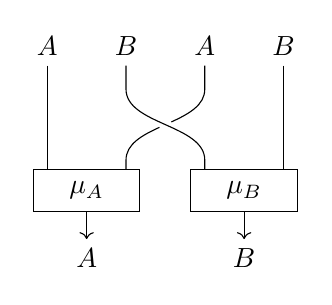
\begin{tikzpicture}[baseline=(braid)]
		\pic[
			braid/number of strands=4,
			braid/every strand/.style={black},
			name prefix=braid
		]
		at (0, 0) {braid = {s_2}};
		\coordinate (braid) at ($(braid-1-s)!0.5!(braid-1-e)$);
		\node[above] at (braid-1-s) {$A$};
		\node[above] at (braid-2-s) {$B$};
		\node[above] at (braid-3-s) {$A$};
		\node[above] at (braid-4-s) {$B$};
		
		\coordinate (MA) at ($(braid-1-e)!0.5!(braid-3-e)$);
		\draw[->] (MA) -- ($(MA) + (0, -2em)$) node[below] {$A$};
		\draw[fill=white] ([yshift=0.5em, xshift=-0.5em] braid-1-e) rectangle ([yshift=-1em, xshift=0.5em] braid-3-e);
		\node at ([yshift=-0.25em] MA) {$\mu_A$};
		
		\coordinate (MB) at ($(braid-2-e)!0.5!(braid-4-e)$);
		\draw[->] (MB) -- ($(MB) + (0, -2em)$) node[below] {$B$};
		\draw[fill=white] ([yshift=0.5em, xshift=-0.5em] braid-2-e) rectangle ([yshift=-1em, xshift=0.5em] braid-4-e);
		\node at ([yshift=-0.25em] MB) {$\mu_B$};
	\end{tikzpicture}\end{center}
	
	\item 幺元 $\eta_{A \otimes B}$ 取为合成
	\[ \munit \xrightarrow[\sim]{\iota^{-1}} \munit \otimes \munit \xrightarrow{\eta_A \otimes \eta_B} A \otimes B. \]
\end{itemize}

为了验证这确实是代数, 定义 \ref{def:algebra-monoidal} 的条件可以简单地运用 $c$ (调换 $\otimes$ 顺序), $\iota$ (复制幺元) 和结合约束 (调整括号顺序) 来化约到 $(A, \mu_A, \eta_A)$ 和 $(B, \mu_B, \eta_B)$ 的对应性质.

若 $M$ 是左 $A$-模, $N$ 是左 $B$-模, 则 $M \otimes N$ 自然地成为左 $A \otimes B$-模; 构造及验证和上一段无异, 需要用到 $c$ 来调换位置. 右模情形亦然.

对于注记 \ref{rem:unit-algebra} 定义的代数 $\munit$, 显然有 $\munit \otimes A \simeq A \simeq A \otimes \munit$, 同构由 $\mathcal{V}$ 的幺约束给出.

\begin{remark}\label{rem:Alg-otimes-functorial}
	上述构造对 $A$, $B$ 具有函子性: 若 $A \to A'$ 和 $B \to B'$ 是代数之间的态射, 则相应的 $A \otimes B \to A' \otimes B'$ 亦然. 另一个繁而不难的事实则是当 $A$, $B$, $C$ 全为代数时, 结合约束 $(A \otimes B) \otimes C \rightiso A \otimes (B \otimes C)$ 是代数之间的态射,
\end{remark}

\begin{lemma}\label{prop:CAlg-mu}
	设 $A$ 是辫幺半范畴 $\mathcal{V}$ 上的代数, 则 $A$ 交换当且仅当 $A$ 的乘法 $\mu_A: A \otimes A \to A$ 是代数之间的态射.
\end{lemma}
\begin{proof}
	为了使 $\mu_A$ 成为代数之间的态射, 需要两则条件. 关于幺元的条件等价于
	\[\begin{tikzcd}[column sep=large]
		\munit \otimes \munit \arrow[d, "\iota"'] \arrow[r, "{\eta_A \otimes \eta_A}"] & A \otimes A \arrow[d, "{\mu_A}"] \\
		\munit \arrow[r, "{\eta_A}"'] & A
	\end{tikzcd}\]
	交换, 既然 $A$ 是代数, 这自动成立. 余下条件则是图表
	\begin{equation*}
		\begin{tikzcd}[column sep=large]
			(A \otimes A) \otimes (A \otimes A) \arrow[r, "{\mu_A \otimes \mu_A}"] \arrow[d, "{\mu_{A \otimes A}}"'] & A \otimes A \arrow[d, "{\mu_A}"] \\
			A \otimes A \arrow[r, "{\mu_A}"'] & A
		\end{tikzcd}
	\end{equation*}
	交换. 将左上角通过结合约束等同于 $A \otimes (A \otimes A) \otimes A$. 根据 $\mu_A$ 的结合律, 图表按
	\begin{tikzpicture}[scale=0.5, baseline=(O)]
		\draw[->] (0, 0) -- (1, 0) -- (1, -0.7);
		\coordinate (O) at (0, -0.5);
	\end{tikzpicture}
	合成等于
	\[ A \otimes (A \otimes A) \otimes A \xrightarrow{\identity \otimes \mu_A \otimes \identity} A \otimes A \otimes A \xrightarrow{\text{相乘}} A . \]
	另一方面, $\mu_{A \otimes A}$ 的定义和 $\mu_A$ 的结合律表明图表按
	\begin{tikzpicture}[scale=0.5, baseline=(O)]
		\draw[->] (0, 0) -- (0, -0.7) -- (1, -0.7);
		\coordinate (O) at (0, -0.5);
	\end{tikzpicture}
	合成等于
	\[ A \otimes (A \otimes A) \otimes A \xrightarrow{\identity \otimes (\mu_A c(A,A) ) \otimes \identity} A \otimes A \otimes A \xrightarrow{\text{相乘}} A . \]
	由此可知 $\mu_A c(A, A) = \mu_A$ 蕴涵原图交换, 亦即 $\mu_A$ 是代数之间的态射.
	
	至于反向蕴涵, 令 $f \in \left\{ \mu_A, \mu_A c(A, A) \right\}$, 则有简单的交换图表
	\[\begin{tikzcd}
		A \otimes (A \otimes A) \otimes A \arrow[r, "{\identity \otimes f \otimes \identity}"] & A \otimes A \otimes A \arrow[r, "{\text{相乘}}"] & A . \\
		A \otimes A \arrow[u, "{\eta_A \otimes \identity \otimes \eta_A}"] \arrow[r, "f"'] & A \arrow[ru, "\identity"'] \arrow[u, "{\eta_A \otimes \identity \otimes \eta_A}"] &
	\end{tikzcd}\]
	若 $\mu_A$ 是代数之间的态射, 则先前讨论说明第一行对 $f$ 的两种选取都给出同样的合成, 再考察第二行即得 $\mu_A = \mu_A c(A, A)$.
\end{proof}

\begin{lemma}\label{prop:c-as-isom-alg}
	设 $A$ 和 $B$ 为对称幺半范畴 $\mathcal{V}$ 上的代数, 则 $c(A, B): A \otimes B \to B \otimes A$ 是代数之间的同构.
\end{lemma}
\begin{proof}
	必须对 $c(A, B)$ 验证两个交换图表. 第一个图表是
	\[\begin{tikzcd}[row sep=tiny]
		& \munit \otimes \munit \arrow[ld, "\sim" sloped] \arrow[dd, "{c(\munit, \munit)}"] \arrow[r, "{\eta_A \otimes_B}"] & A \otimes B \arrow[dd, "{c(A, B)}"] \\
		\munit & & \\
		& \munit \otimes \munit \arrow[lu, "\sim"' sloped] \arrow[r, "{\eta_B \otimes \eta_A}"'] & B \otimes A
	\end{tikzcd}\]
	右部交换归结于 $c$ 的函子性, 左部交换归结为 $c$ 和幺约束相容 \cite[(3.12)]{Li1}. 关于 $c(A, B)$ 保乘法的第二个图表, 其论证是基于辫结构的对称性, 和 \cite[\S 7.4]{Li1} 结尾处完全相同.
\end{proof}

\begin{proposition}
	设 $A$ 和 $B$ 是对称幺半范畴 $\mathcal{V}$ 上的交换代数, 则 $A \otimes B$ 亦然.
\end{proposition}
\begin{proof}
	说明乘法 $\mu_{A \otimes B}$ 是代数之间的态射即可. 回顾 $\mu_{A \otimes B}$ 的定义, 并应用引理 \ref{prop:c-as-isom-alg} (处理 $c(B, A)$), 关于 $A$, $B$ 交换的前提 (用引理 \ref{prop:CAlg-mu} 处理 $\mu_A$, $\mu_B$), 和关于 $\otimes$ 的函子性的注记 \ref{rem:Alg-otimes-functorial}, 可知其中每一段都是代数之间的态射.
\end{proof}

以上定义了代数, 模和其间的态射. 这些结构皆可作成范畴, 记法为
\begin{center}\begin{tabular}{|c|c|c|c|c|c|} \hline
	结构 & 代数 & 交换代数 & 左 $A$-模 & 右 $B$-模 & $(A,B)$-双模 \\ \hline
	所成范畴 & $\cate{Alg}(\mathcal{V})$ & $\cate{CAlg}(\mathcal{V})$ & $A\dcate{Mod}$ & $\cated{Mod}B$ & $(A,B)\dcate{Mod}$ \\ \hline
	条件 & {\small $\mathcal{V}$: 幺半范畴} & {\small $\mathcal{V}$: 辫幺半范畴} & {\small $A$: 代数} & {\small $B$: 代数} & {\small $A, B$: 代数} \\ \hline
\end{tabular}\end{center}
\index[sym1]{Alg@$\cate{Alg}(\cdot)$}
\index[sym1]{CAlg@$\cate{CAlg}(\cdot)$}
\index[sym1]{Mod}

上述讨论还指明 $\cate{Alg}(\mathcal{V})$ 和 $\cate{CAlg}(\mathcal{V})$ 的结构一般要少于 $\mathcal{V}$, 以数字标注结构多寡, 则可约略图解为
\[\begin{tikzcd}[row sep=small]
	0 & 1 & 2 & \infty \\
	\text{范畴} & \text{幺半范畴} \arrow[l, "{\cate{Alg}}"'] & \text{辫幺半范畴} \arrow[shift right, l, "{\cate{Alg}}"'] \arrow[shift left, bend left, ll, "{\cate{CAlg}}"'] & \text{对称幺半范畴} \arrow[loop right, "{\cate{Alg}, \cate{CAlg}}"]
\end{tikzcd}\]
此外, 只要 $\cate{Alg}(\mathcal{V})$ 或 $\cate{CAlg}(\mathcal{V})$ 对 $\otimes$ 成幺半范畴, 则它总以 $\munit$ 为幺元.

回忆到引理 \ref{prop:CAlg-mu} 说明辫幺半范畴 $\mathcal{V}$ 上的交换代数自动给出幺半范畴 $\cate{Alg}(\mathcal{V})$ 上的代数, 方式是取 $A \otimes A \to A$ 为 $A$ 的乘法. 事实上这是唯一可能的取法, 而且由此引出一则简单, 有趣且重要的观察: 我们有范畴的等价
\begin{equation}\label{eqn:AlgAlg-CAlg}
	\cate{Alg}\left(\cate{Alg}(\mathcal{V}) \right) \simeq \cate{CAlg}(\mathcal{V}), \quad \mathcal{V}:\;\text{辫幺半范畴}.
\end{equation}
这些事实是基于所谓的 \emph{Eckmann--Hilton 论证}, 谨留作附有提示的本章习题.

\begin{example}\label{eg:Cartesius-monoidal}
	设范畴 $\mathcal{C}$ 具备有限积; 特别地, 存在空积, 亦即终对象, 记为 $\munit$; 对任两个对象 $X, Y$ 都有典范同构 $c(X, Y): X \times Y \rightiso Y \times X$. 由此将 $(\mathcal{C}, \times)$ 作成以 $\munit$ 为幺元的对称幺半范畴. 依此探讨 $\mathcal{C}$ 上的代数, 或称 $\mathcal{C}$ 上的幺半群对象\footnote{对于这类范畴, \cite[\S 4.11]{Li1} 还探讨了群对象, 但其中的逆元性质无法在一般的幺半范畴中表述.}, 及其交换版本.
	\begin{itemize}
		\item 取 $\mathcal{C} = \cate{Set}$, 则独点集为幺元 $\munit$. 对应的代数是幺半群, 对应的交换代数则是交换幺半群.
		\item 取 $\mathcal{C} = \cate{Top}$, 则对应的代数是拓扑幺半群, 对应的交换代数是交换拓扑幺半群.
	\end{itemize}

	另一方面, 取交换环 $\Bbbk$, 以 $\otimes = \otimes_{\Bbbk}$ 赋予 $\Bbbk\dcate{Mod}$ 对称幺半范畴的结构, 以 $\Bbbk$ 为幺元 $\munit$, 以 $x \otimes y \mapsto y \otimes x$ 确定辫结构, 则对应的代数 (或交换代数) 即是代数意义下的代数 (或交换代数), 见 \cite[定义 7.1.1]{Li1}.
\end{example}

在这些具体情境下, 代数 $A$ 的乘法往往直接写成元素相乘 $xy = x \cdot y$, 幺元直接等同于元素 $1_A$, 可以省去 $\mu_A$, $\eta_A$ 等符号.

\begin{example}[分次模与分次代数]\label{eg:graded-module}
	\index{fencimo@分次模, 分次代数 (graded module, graded algebra)}
	取定 Abel 范畴 $\mathcal{A}$ 和非空集 $I$. 我们称 $\mathcal{A}^I$ 的对象为 $I$-分次对象, 表作 $M = (M^i)_{i \in I}$ 之形, 其间的态射则表作 $(f^i: M^i \to N^i)_{i \in I}$; 习惯称 $M^i \in \Obj(\mathcal{A})$ (或 $f^i \in \Mor(\mathcal{A})$) 为 $M$ (或 $f$) 的 $i$ 次项. 对于 $I = \Z$ 或 $\Z^n$ 的特例, 这在 \S\ref{sec:additive-cplx}, \S\ref{sec:triangular-def}, \S\ref{sec:grading-filtration} 等处已经反复说明.
	
	具体起见, 暂取 $\mathcal{A} := \Bbbk\dcate{Mod}$, 其中 $\Bbbk$ 是交换环; $\mathcal{A}$ 的 $I$-分次对象又称 $I$-分次模. 以下设 $I$ 为幺半群, 在范畴 $\mathcal{A}^I$ 上定义双函子 $\otimes$ 如下:
	\begin{equation}\label{eqn:graded-module}
		(M \otimes N)^i := \bigoplus_{jk=i} M^j \otimes N^k, \quad (f \otimes g)^i := \bigoplus_{jk=i} f^j \otimes g^k .
	\end{equation}
	另外定义 $\munit$ 为集中在 $i = 1_I$ (即 $I$ 的幺元) 项的 $\Bbbk$. 这些资料使得 $\mathcal{A}^I$ 成为幺半范畴. 关于幺元的条件 $\eta_A: \munit = \Bbbk \to A$ 自动确保 $1_A := \eta_A(1) \in A^0$.
	
	对于 $I$ 交换的特例, 我们回归 \cite[定义 7.4.1]{Li1} 介绍的 $I$-分次模和 $I$-分次代数.

	依然设 $\mathcal{A} = \Bbbk\dcate{Mod}$, 并要求 $(I, +)$ 为交换幺半群. 任何加法同态 $\epsilon: I \to \Z/2\Z$ 都使 $\Bbbk\dcate{Mod}^I$ 成为对称幺半范畴, 具有下式所刻画的 \emph{Koszul 辫结构}:
	\begin{equation}\label{eqn:Koszul-braiding}\begin{aligned}
		M^a \otimes N^b & \to N^b \otimes M^a \\
		x \otimes y & \mapsto (-1)^{\epsilon(a)\epsilon(b)} y \otimes x ,
	\end{aligned}\end{equation}
	其中 $a, b \in I$. 对应的交换代数即是 \cite[定义 7.4.3]{Li1} 所称的 $\epsilon$-交换代数. 由此衍生的各种等式或定义统称为 \emph{Koszul 符号律}. 每当交换张量位置时都须依此变号.
	\index{Koszul fuhaolv@Koszul 符号律 (Koszul sign rule)}
	
	举例明之, 使 $A$ 成为交换代数的条件具体写作
	\[ x y = (-1)^{\epsilon(a) \epsilon(b)} yx, \quad x \in A^a, \; y \in A^b. \]
	
	典型场景是
	\[ I \in \{\Z, \Z_{\geq 0} \}, \quad \epsilon(a) := a \;\bmod 2 , \]
	对应的 $\epsilon$-交换代数在前引书中被称为反交换分次代数; 由于这一辫结构在 $\Z$-分次对象的研究中处处出现, 改称\emph{分次交换}是实至名归的.
	
	现在回到更一般的 Abel 范畴 $\mathcal{A}$ 和如上的 $(I, +, \epsilon)$, 为了推广上述构造, 所需的是将 $\mathcal{A}$ 扩充为对称幺半范畴 $(\mathcal{A}, \otimes)$, 使得
	\begin{itemize}
		\item $\mathcal{A}$ 是 Abel 范畴, 形如 \eqref{eqn:graded-module} 的余积 (亦即直和) 存在,
		\item $\otimes: \mathcal{A} \times \mathcal{A} \to \mathcal{A}$ 对每个变元都是加性函子.
	\end{itemize}
	此时 $\mathcal{A}^I$ 上的 $\otimes$ 和 Koszul 辫结构仍可按相同方式定义, 使 $(\mathcal{A}^I, \otimes)$ 成为对称幺半范畴. 它的幺元仍由 $\mathcal{A}$ 的幺元 $\munit$ 给出, 视作集中在零次项的 $I$-分次对象.
	
	对于一般的 $(\mathcal{A}, \otimes)$, 一切验证和 $\Bbbk\dcate{Mod}$ 的情形无异. 唯一差别是在一般情形下, 对象的``元素''不再有意义. 
\end{example}

\begin{convention}
	对于 $\mathcal{A} = \Bbbk\dcate{Mod}$ 的特例, 通行的惯例是将 $I$-分次模 $(M^i)_{i \in I}$ 看作带有直和分解 $M = \bigoplus_{i \in I} M^i$ 的模, 其间的态射要求保持直和项.
\end{convention}

\begin{example}\label{eg:superspace}
	\index{chaoxiangliangkongjian@超向量空间 (super vector space)}
	在上述构造中 ($\mathcal{A} = \Bbbk\dcate{Mod}$) 取 $\Bbbk$ 为满足 $\mathrm{char}(\Bbbk) \neq 2$ 的域, $I = \Z/2\Z = \{0, 1\}$ 而 $\epsilon = \identity_{\Z/2\Z}$. 对应的对称幺半范畴记为 $\cate{Vect}^-_{\Z/2\Z}(\Bbbk)$, 其对象可视同带有直和分解 $V = V_0 \oplus V_1$ 的 $\Bbbk$-向量空间, 又称为\emph{超向量空间}, 由此就产生了线性代数和数学物理中常见的超代数, 交换超代数等种种说法.
\end{example}

最后来讨论松幺半函子对代数的效果.

\begin{definition}\label{def:lax-monoidal}
	\index{hanzi!幺半, 松幺半, 右松幺半 (monoidal, lax monoidal, right lax monoidal)}
	设 $\mathcal{V}$ 和 $\mathcal{V}'$ 为幺半范畴. 根据 \cite[注记 3.1.8]{Li1}, 从 $\mathcal{V}$ 到 $\mathcal{V}'$ 的右松幺半函子, 在此简称\emph{松幺半函子}, 意谓资料 $(F, \xi_F, \varphi_F)$, 其中 $F: \mathcal{V} \to \mathcal{V}$ 是函子, 而态射
	\[ \xi_F: F(\cdot) \otimes F(\cdot) \to F(\cdot \otimes \cdot), \quad \varphi_F: \munit_{\mathcal{V}'} \to F\left( \munit_{\mathcal{V}} \right), \]
	服从于一系列和幺半结构的相容条件. 资料 $(F, \xi_F, \varphi_F)$ 经常简记为 $F$.
	
	若 $\mathcal{V}$ 和 $\mathcal{V}'$ 都是辫 (或对称) 幺半范畴, 而 $F$ 进一步使下图交换, 则称 $F$ 是辫函子, 或者称它兼容于辫结构:
	\[\begin{tikzcd}[column sep=huge]
		F(X) \otimes F(Y) \arrow[r, "{\xi_F(X, Y)}"] \arrow[d, "{c'(FX, FY)}"'] & F(X \otimes Y) \arrow[d, "{Fc(X, Y)}"] \\
		F(Y) \otimes F(X) \arrow[r, "{\xi_F(Y, X)}"'] & F(Y \otimes X) .
	\end{tikzcd}\]

	若松幺半函子资料中的 $\xi_F$ 和 $\varphi_F$ 皆为同构, 则称之为\emph{幺半函子}.
\end{definition}

当然, 我们还可以进一步探讨从松幺半函子之间的态射, 或称自然变换:
\[ \theta = (\theta_X)_{X \in \Obj(\mathcal{V})}: F \to G, \quad F, G: \mathcal{V} \to \mathcal{V}' . \]
除了自然变换所需的条件, 我们还要求 $\theta$ 使下图交换:
\[\begin{tikzcd}[column sep=huge]
	F(X) \otimes F(Y) \arrow[r, "{\xi_F(X, Y)}"] \arrow[d, "{\theta_X \otimes \theta_Y}"'] & F(X \otimes Y) \arrow[d, "{\theta_{X \otimes Y}}"] \\
	G(X) \otimes G(Y) \arrow[r, "{\xi_G(X, Y)}"'] & G(X \otimes Y)
\end{tikzcd} \quad \begin{tikzcd}
	\munit_{\mathcal{V}'} \arrow[r, "{\varphi_F}"] \arrow[rd, "{\varphi_G}"'] & F(\munit_{\mathcal{V}}) \arrow[d, "{\theta_{\munit_{\mathcal{V}}}}"] \\
	& G(\munit_{\mathcal{V}}) .
\end{tikzcd}\]

当 $F$ 和 $G$ 为幺半函子时, 上述定义实则等价于 \cite[定义 3.1.10]{Li1}; 此处的 $\varphi_F$ 和 $\varphi_G$ 在该处被称作``标准''同构. 由此遂可探讨幺半范畴或辫幺半范畴之间的等价.

\begin{proposition}\label{prop:lax-monoidal-Alg}
	松幺半函子 $F$ 诱导函子 $\cate{Alg}(\mathcal{V}) \to \cate{Alg}(\mathcal{V}')$; 若 $A$ 是 $\mathcal{V}$ 上的代数, 则 $F$ 诱导 $A\dcate{Mod} \to F(A) \dcate{Mod}$, 依此类推.

	若进一步要求 $\mathcal{V}$ 和 $\mathcal{V}'$ 是辫幺半范畴, 而 $F$ 是辫函子, 则 $F$ 还诱导 $\cate{CAlg}(\mathcal{V}) \to \cate{CAlg}(\mathcal{V}')$, 而且此时 $\cate{Alg}(\mathcal{V}) \to \cate{Alg}(\mathcal{V}')$ 是松幺半函子; 若进一步要求 $\mathcal{V}, \mathcal{V}'$ 皆对称, 则 $\cate{CAlg}(\mathcal{V}) \to \cate{CAlg}(\mathcal{V}')$ 亦然.
\end{proposition}
\begin{proof}
	设 $A$ 为 $\mathcal{V}$ 上的代数. 乘法 $\mu_{FA}$ 定为 $FA \otimes FA \to F(A \otimes A) \xrightarrow{F\mu_A} FA$, 幺元 $\eta_{FA}$ 定为 $\munit_{\mathcal{V}'} \to F(\munit_{\mathcal{V}}) \xrightarrow{F\eta_A} FA$. 其余验证全是例行公事.
\end{proof}

\begin{example}\label{eg:ev0-monoidal}
	考虑例 \ref{eg:graded-module} 中的对称幺半 Abel 范畴 $\mathcal{A}$ 和 $\mathcal{A}^I$. 定义函子
	\[ \mathrm{ev}_0: \mathcal{A}^I \to \mathcal{A}, \quad \left(M^i\right)_{i \in I} \mapsto M^0. \]
	这是正合函子, 同时也是对称松幺半函子: 仅须取
	\[ \xi_{\mathrm{ev}_0}(M, N): M^0 \otimes N^0 \to (M \otimes N)^0 := \bigoplus_{i+j=0} M^i \otimes N^j \]
	为自明的态射, 而 $\varphi_{\mathrm{ev}_0}: \munit \to \munit$ 是恒等. 于是 $A \mapsto A^0$ 便诱导松幺半函子
	\[ \cate{Alg}(\mathcal{A}^I) \to \cate{Alg}(\mathcal{A}), \quad \cate{CAlg}(\mathcal{A}^I) \to \cate{CAlg}(\mathcal{A}). \]
\end{example}

下一则注记探讨一般的幺半范畴 $\mathcal{V}$ 上的代数. 回忆到有限序数和 $\Z_{\geq 0}$ 一一对应, $n$ 对应的有限序数 $\mathbf{n}$ 等同于含 $n$ 个元素的全序集 $\{0, \ldots, n-1\}$, 其中 $0 \leq 1 \leq 2 \leq \cdots$.

\begin{remark}[游走代数]\label{rem:walking-algebra}
	\index{daishu!游走 (walking)}
	\index[sym1]{FinOrd@$\cate{FinOrd}$}
	偏序集之间的映射 $f: A \to B$ 若满足 $a \leq a' \implies f(a) \leq f(a')$, 则称为保序的. 今后记 $\cate{FinOrd}$ 为有限序数范畴, 态射是序数之间的保序映射. 它对 $\mathbf{n} \otimes \mathbf{m} := \mathbf{n} + \mathbf{m}$ 成为严格幺半范畴, 态射 $f \otimes g: \mathbf{n} \otimes \mathbf{m} \to \mathbf{n}' \otimes \mathbf{m}'$ 将前 $n$ 个 (或后 $m$ 个) 元素以 $f$ (或 $g$) 映射, 对象 $\mathbf{0}$ 为幺元\footnote{此处 $\mathbf{1}$ 均指序数; 幺半范畴 $\mathcal{V}$ 的幺元另记为 $\munit_{\mathcal{V}}$.}. 将 $\mathbf{1}$ 作成 $\cate{FinOrd}$ 上的代数: 取幺元为 $\emptyset = \mathbf{0} \hookrightarrow \mathbf{1}$ 而乘法为 $\mathbf{1} \otimes \mathbf{1} = \mathbf{2} \twoheadrightarrow \mathbf{1}$, 相关交换图表的验证没有丝毫困难.
	
	序数 $\mathbf{1}$ (或 $\mathbf{2}$) 可视同``游走''的对象 (或态射), 这是因为对任意范畴 $\mathcal{C}$, 指定函子 $\mathbf{1} \to \mathcal{C}$ (或 $\mathbf{2} \to \mathcal{C}$) 相当于指定 $\mathcal{C}$ 的对象 (或态射). 现在考虑幺半范畴 $\mathcal{V}$. 兹断言有范畴之间的同构
	\[
		\left\{ \mathcal{V}\;\text{上的代数}\; A \right\} \simeq \left\{ \text{幺半函子}\; F: \cate{FinOrd} \to \mathcal{V} \right\},
	\]
	这也相当于说 $\cate{FinOrd}$ 是``游走的代数''. 首先, 对幺半函子 $F: \cate{FinOrd} \to \mathcal{V}$ 定义 $A := F(\mathbf{1})$, 作为命题 \ref{prop:lax-monoidal-Alg} 的简单特例, $A$ 自然地成为 $\mathcal{V}$ 上的代数: $\mu: A \otimes A \to A$ 是 $F(\mathbf{2} \twoheadrightarrow \mathbf{1})$, 而 $\eta: \munit_{\mathcal{V}} \to A$ 是 $F(\mathbf{0} \hookrightarrow \mathbf{1})$.
	
	反之给定 $\mathcal{V}$ 上的代数 $(A, \mu, \eta)$, 定义幺半函子 $F: \cate{FinOrd} \to \mathcal{V}$ 使得
	\[ F(\mathbf{n}) = A^{\otimes n} := \underbracket{A \otimes (A \otimes (\cdots))}_{n\;\text{份}\; A}, \quad A^{\otimes 0} := \munit_{\mathcal{V}}, \]
	对于 $f: \mathbf{n} \to \mathbf{m}$, 若 $f$ 单则 $F(f): A^{\otimes n} \to A^{\otimes m}$ 相当于在 $f$ 的值域之外补上 $\eta: \munit_{\mathcal{V}} \to A$, 若 $f$ 满则 $F(f)$ 相当于用 $\mu: A \otimes A \to A$ 逐步合并纤维里的项; 幺半范畴的结合约束等性质说明这些运算良定义. 一般的 $f$ 可以唯一地作满--单分解, 依此在对象层次定义 $F$. 它在态射层次的定义则是明白的. 不难验证双向构造互逆.
\end{remark}

\section{实例: 微分分次结构}\label{sec:dga-monoidal}
承接例 \ref{eg:graded-module} 的讨论, 考虑具有可数余积的对称幺半 Abel 范畴 $(\mathcal{A}, \otimes)$. 本节进一步假定 $\otimes$ 对每个变元都是右正合的. 典型例子自然是 $\mathcal{A} = \Bbbk\dcate{Mod}$.

先前已经讨论 $\mathcal{A}$ 上的 $\Z$-分次代数, 或者说是幺半范畴 $(\mathcal{A}^{\Z}, \otimes)$ 上的代数; 精确地说, 这在例 \ref{eg:graded-module} 的框架下相当于取 $I = \Z$ 和 $\epsilon(a) = a \bmod\; 2$ 所对应的 Koszul 辫结构 \eqref{eqn:Koszul-braiding}. 以下将 $\Z$-分次简称为分次. 本节的重点是加入``微分''结构; 相关内容和 \S\ref{sec:multiplicative-SS} 略有重叠.

平移函子 $T: \mathcal{A}^{\Z} \to \mathcal{A}^{\Z}$ 定义为 $(TM)^n = M^{n+1}$, $(Tf)^n = f^{n+1}$; 这使 $\left(\mathcal{A}^{\Z}, T\right)$ 成为带平移的 Abel 范畴, 其上的微分对象 (定义 \ref{def:differential-object}) 简称 $\mathcal{A}$ 上的\emph{微分分次对象}. 事实上, 微分分次对象构成的 Abel 范畴 $\left(\mathcal{A}^{\Z}, T\right)_d$ 典范地同构于复形范畴 $\cate{C}(\mathcal{A})$. 这是在 \S\ref{sec:additive-cplx} 便已知晓的事实.
\index{weifenfenciduixiang}

有鉴于此, 今后将不加区分地等同 $\mathcal{A}$ 上的微分分次对象和复形.

现在赋予 $\cate{C}(\mathcal{A})$ 对称幺半范畴的结构. 对任意复形 $M$ 和 $N$, 双函子 $\otimes: \mathcal{A} \times \mathcal{A} \to \mathcal{A}$ 给出双复形 $M^\bullet \otimes N^\bullet$, 再以直和取全复形得出
\[ M \otimes N := \tot_{\oplus}\left( M^\bullet \otimes N^\bullet \right), \quad (M \otimes N)^n = \bigoplus_{a+b=n} M^a \otimes N^b. \]

对于 $\mathcal{A} = \Bbbk\dcate{Mod}$ 的实例, 复形 (或等价地说, 微分对象) 的微分态射 $d = d_{M \otimes N}$ 在元素的层次写作
\begin{equation*}
	d(x \otimes y) = (d_M x) + (-1)^a x (d_N y), \quad x \in M^a, \; y \in N^b.
\end{equation*}
这些定义使 Koszul 辫结构 \eqref{eqn:Koszul-braiding} 给出复形之间的态射; 请读者直接验证, 或归结为命题 \ref{prop:double-cplx-swap}.

此外, $(\mathcal{A}, \otimes)$ 的幺元 $\munit$ 作为集中在零次项的复形, 显然给出幺半范畴 $(\cate{C}(\mathcal{A}), \otimes)$ 的幺元. 以下事实是明白的: 对任意 $X = (X^n, d_X^n)_n \in \Obj(\cate{C}(\mathcal{A}))$, 我们有
\begin{equation}\label{eqn:unit-map-into-cplx}
	\Hom_{\cate{C}(\mathcal{A})}(\munit, X) \simeq \Hom_{\mathcal{A}}\left( \munit, \Ker\left(d_X^0 \right) \right).
\end{equation}

\begin{definition}\label{def:dg-algebra}
	\index{weifenfencidaishu}
	\index{dg daishu}
	相对于前述对称幺半结构, 我们将 $\cate{Alg}\left(\cate{C}(\mathcal{A})\right)$ 的对象称为 $\mathcal{A}$ 上的\emph{微分分次代数}, 简称 \emph{dg-代数}, 而 $\cate{CAlg}\left(\cate{C}(\mathcal{A})\right)$ 的对象则称为 $\mathcal{A}$ 上的交换微分分次代数, 简称交换 dg-代数.
\end{definition}

由此起步, 也可以对给定的微分分次代数 $A$ 探讨左 (或右) $A$-模 $M$, 乃至于双模; 它们都构成 Abel 范畴. 此时也称 $M$ 是 $A$ 上的\emph{微分分次模}, 简称 \emph{dg-模}. 这是复形与模论的综合体, 用途广泛, 本章习题将有更多介绍, 读者也可以参阅 \cite{Yek20} 等专著. 为了突出微分分次结构, 今后将 dg-模构成的范畴另记为 $A\dcate{dgMod}$, 依此类推.
\index{weifenfencimo@微分分次模 (differential graded module)}
\index{dg mo@dg-模}
\index[sym1]{A-dgMod@$A\dcate{dgMod}$}

忘却函子 $\cate{C}(\mathcal{A}) \to \mathcal{A}^{\Z}$ 保 $\otimes$, 故命题 \ref{prop:lax-monoidal-Alg} 说明它保持代数 (或交换代数) 的结构. 对于 $\mathcal{A} = \Bbbk\dcate{Mod}$ 的情形, 说 $A$ 是 dg-代数相当于说 $A$ 本身是分次代数, 带有微分态射 $d$, 而且其乘法服从 Leibniz 律
\[ d(xy) = (dx)y + (-1)^a x (dy), \quad x \in A^a, \; y \in A^b. \]
代入 $x = 1_A = y$ 遂有 $d(1_A) = 0$. 对应的相反代数 $A^{\opp}$ 相当于将乘法改成 $x \cdot^{\opp} y := (-1)^{ab} y x$.

类似地, 当 $\mathcal{A} = \Bbbk\dcate{Mod}$ 时, 左 $A$-模 $M$ 相当于一个分次 $\Bbbk$-模 $M$ 连同纯量乘法态射 $A \otimes M \to M$, 满足结合律等种种性质, 并且带有微分态射 $d$, 服从 Leibniz 律
\[ d(tm) = (dt)m + (-1)^a t (dm), \quad t \in A^a, \; m \in M^b; \]
对于右 $A$-模 $M$, Leibniz 律变为
\[ d(mt) = (dm)t + (-1)^b m (dt), \quad t \in A^a, \; m \in M^b. \]
对于一般的 $(\mathcal{A}, \otimes)$, 上述性质皆有不涉及元素的表述方式, 譬如代数 $A$ 的幺元对应到 $\mathcal{A}$ 的态射 $\munit \to \Ker\left(d_A^0\right)$, 见 \eqref{eqn:unit-map-into-cplx}.

取上同调给出加性函子 $\Hm = \left( \Hm^n \right)_{n \in \Z}: \cate{C}(\mathcal{A}) \to \mathcal{A}^{\Z}$. 以下结果表明复形的乘法诱导上同调的乘法.

\begin{proposition}\label{prop:Hm-lax-monoidal}
	函子 $\Hm$ 诱导
	\[ \cate{Alg}\left(\cate{C}(\mathcal{A})\right) \to \cate{Alg}\left(\mathcal{A}^{\Z}\right),
	\quad \cate{CAlg}\left(\cate{C}(\mathcal{A})\right) \to \cate{CAlg}\left(\mathcal{A}^{\Z}\right). \]
	若 $A$ 是 dg-代数, 而 $M$ 是左 (或右, 或双) $A$-模, 则 $\Hm(M)$ 是左 (或右, 或双) $\Hm(A)$-模.
\end{proposition}
\begin{proof}
	鉴于命题 \ref{prop:lax-monoidal-Alg}, 说明 $\Hm$ 是松幺半函子即可. 所需的典范态射
	\[ \xi_{\Hm}(M, N): \Hm(M) \otimes \Hm(N) \to \Hm(M \otimes N) \]
	近乎自明: 它来自定理 \ref{prop:Kunneth-homology} 或命题 \ref{prop:bifunctor-cup} 之上论及的态射 $\kappa$. 另一方面,
	\[ \varphi_{\Hm}: \munit \to \Hm(\munit) = \munit \quad \text{(集中于零次项)} \]
	则取为 $\identity$.
\end{proof}

我们还可以进一步取例 \ref{eg:ev0-monoidal} 的松幺半函子 $\mathrm{ev}_0: \mathcal{A}^{\Z} \to \mathcal{A}$; 同样由命题 \ref{prop:lax-monoidal-Alg} 可知这映分次代数 (或交换分次代数) 为代数 (或交换代数), 映模为模. 留意到 $\mathrm{ev}_0 \Hm = \Hm^0$. 实际应用中, $\cate{C}(\mathcal{A}) \xrightarrow{\Hm} \mathcal{A}^{\Z} \xrightarrow{\mathrm{ev}_0} \mathcal{A}$ 在每一段都会丢失信息, 最丰富的结构仍在 dg-代数本身.

\begin{example}\label{eg:k-linear-A-enrich}
	设 $\Bbbk$ 为交换环. 对于任意 $\Bbbk$-线性范畴 $\mathcal{A}$, 考虑 $\Hom$ 复形层次的乘法 \eqref{eqn:Hom-cplx-multiplication}:
	\[ \Hom^a(Y, Z) \times \Hom^b(X, Y) \to \Hom^{a+b}(X, Z), \quad X, Y, Z \in \Obj(\cate{C}(\mathcal{A})). \]
	
	由于乘法满足 Leibniz 律 (引理 \ref{prop:Hom-cplx-Leibniz}), 它确定 $\cate{C}(\Bbbk\dcate{Mod})$ 的态射
	\[ \Hom^\bullet(Y, Z) \otimes \Hom^\bullet(X, Y) \to \Hom^\bullet(X, Z). \]
	此外它还具有结合律, 于是 $\End^\bullet(X) := \Hom^\bullet(X, X)$ 成为 $(\cate{C}(\Bbbk\dcate{Mod}), \otimes)$ 上的代数, 以 $\identity_X \in \End^0(X)$ 为其幺元. 进一步, $\Hom^\bullet(X, Y)$ 成为 $(\End^\bullet(Y), \End^\bullet(X))$-双模.
	
	取 $\Hom^\bullet(X, Y)$ 的上同调 $\Hm = (\Hm^n)_n$, 产物只是
	\[ \bigoplus_{n \in \Z} \Hom_{\cate{K}(\mathcal{A})}(X, Y[n]); \]
	而对 $\Hom^\bullet(X, Y)$ 应用 \eqref{eqn:unit-map-into-cplx} 可见 $\Hom_{\cate{C}(\mathcal{A})}$ 可以通过
	\[ \Hom_{\cate{C}(\Bbbk\dcate{Mod})}\left( \Bbbk, \Hom^\bullet(X, Y) \right) \simeq \Hom_{\cate{C}(\mathcal{A})}(X, Y)  \]
	来重构, 此处 $\Bbbk$ 充当了 $(\cate{C}(\Bbbk\dcate{Mod}), \otimes)$ 的幺元.
\end{example}

因此 $\cate{C}(\mathcal{A})$ 中的 $\Hom_{\cate{C}(\mathcal{A})}$ 及态射合成仅是 $\Hom$ 复形及其乘法的一道影子, 来自于取 $\Hom_{\cate{C}(\Bbbk\dcate{Mod})}(\Bbbk, \cdot)$.

\index{fanchou!充实 (enriched)}
\index[sym1]{Hom-internal@$\iHom$}
由 $\cate{C}(\mathcal{A})$ 的例子入手, 自然地提炼出微分分次范畴的概念. 这涉及 \cite[定义 3.4.1]{Li1} 介绍的 $\mathcal{V}$-\emph{充实范畴}. 简言之, 对任意幺半范畴 $\mathcal{V}$, 一个 $\mathcal{V}$-充实范畴 $\mathcal{C}$ 仍由对象和态射组成, 然而 $\Hom$ 集须代换为 $\mathcal{V}$ 中的 $\Hom$ 对象, 记为 $\iHom = \iHom_{\mathcal{C}}$ 以资区别; 态射的合成代换为 $\mathcal{V}$ 的态射
\[ \iHom(Y, Z) \otimes \iHom(X, Y) \to \iHom(X, Z), \]
而恒等态射 $\identity_X \in \Hom(X, X)$ 代换为 $\identity_X: \munit \to \iHom(X, X)$, 这些都是 $\mathcal{V}$ 的态射, 相应的性质都由 $\mathcal{V}$ 的交换图表表述.

关于充实版本的函子及其间的态射, 详见 \cite[定义 3.4.1, 3.4.2, 3.4.4]{Li1}, 它们都是按显然方式定义的; 简言之, 充实版本的函子将 $\Hom$ 集之间的映射升级为 $\iHom$ 之间的态射.

举例明之, $\Bbbk\dcate{Mod}$-范畴无非是 $(\Bbbk\dcate{Mod}, \otimes)$-充实范畴.

与此相对, 姑且将未充实的范畴称作普通范畴. 倘若略去集合大小的问题, 则普通范畴也相当于 $(\cate{Set}, \times)$-充实范畴.

\begin{definition}\label{def:dgCat}
	\index{fanchou!微分分次 (differential graded)}
	\index{dgfanchou@dg-范畴}
	设 $\Bbbk$ 为交换环. 考虑相应的对称幺半范畴 $(\cate{C}(\Bbbk\dcate{Mod}), \otimes)$, 则 $(\cate{C}(\Bbbk\dcate{Mod}), \otimes)$-充实范畴称为 $\Bbbk$ 上的\emph{微分分次范畴}, 简称 $\Bbbk$ 上的 \emph{dg-范畴}. 这些范畴之间的函子及函子之间的态射按充实范畴的方式定义\footnote{许多涉及无穷范畴的文献提及了 DG-范畴以及它们构成的范畴 $\cate{DGCat}$, 有时符号也和本书重叠; 尽管它们和此处铺陈的 dg-范畴密切相关, 但并非一回事.}.
\end{definition}

按定义, dg-范畴的对象 $X$ 给出 dg-代数 $\End^\bullet(X)$.

\begin{example}\label{eg:CA-dg-cat}
	先前的例 \ref{eg:k-linear-A-enrich} 相当于说 $\cate{C}(\mathcal{A})$ 自然地成为 $\Bbbk$ 上的 dg-范畴, 此处 $\mathcal{A}$ 是任意 $\Bbbk$-线性范畴. 譬如对于任何 $\Bbbk$-代数 $R$, 左 (或右) $R$-模的复形范畴自动是 $\Bbbk$ 上的 dg-范畴.
\end{example}

\begin{example}\label{eg:dg-Hom-cplx}
	\index{Hom fuxing}
	\index[sym1]{Hom-A-bullet@$\Hom^{\bullet}_A$}
	设 $\Bbbk$ 为交换环, $A$ 为 $\mathcal{A} := \Bbbk\dcate{Mod}$ 上的 dg-代数. 对于左 $A$-模 $M$ 和 $N$, 定义 $\Hom^\bullet_{\Bbbk}(M, N)$ 的子复形如下
	\[ \Hom^p_A(M, N) := \left\{\begin{array}{r|l}
		f \in \Hom^p_{\Bbbk}(M, N) & \forall m \in M, \; \forall k \in \Z, \; \forall t \in A^k, \\
		& f(tm) = (-1)^{pk} tf(m)
	\end{array}\right\}. \]
	给定左 $A$-模 $L$, $M$, $N$, 复形 $\Hom^\bullet_{\Bbbk}$ 上的合成运算诱导复形之间的态射
	\[ \Hom^p_A(M, N) \otimes \Hom^q_A(L, M) \to \Hom^{p+q}_A(L, N). \]
	这使左 $A$-模范畴 $A\dcate{dgMod}$ 升级为 dg-范畴. 对于右 $A$-模, $\Hom^p_A(M, N)$ 定义中的条件应当改为 $f(mt) = f(m)t$ (思之). 双模的情形依此类推.
	
	上述定义也有不依赖于集合元素的表法, 因而可以扩及一般的 $\mathcal{A}$.
\end{example}

更精确地说, dg-范畴将普通范畴的 $\Hom$ 集全部升级为复形 $\Hom^\bullet$, 而 dg-版本的函子与态射皆须在 $\cate{C}(\Bbbk\dcate{Mod})$ 中表述. 详言之,
\begin{itemize}
	\item dg-范畴之间的 \emph{dg-函子} $F: \mathcal{C} \to \mathcal{D}$ 由对象集之间的映射 $F: \Obj(\mathcal{C}) \to \Obj(\mathcal{D})$ 和 $\Hom$ 复形之间的态射 $\Hom^\bullet_{\mathcal{C}}(X, Y) \to \Hom^\bullet_{\mathcal{D}}(FX, FY)$ 确定, 后者是 $\cate{C}(\Bbbk\dcate{Mod})$ 的态射, 要求使以下两个图表交换:
	\begin{equation*}\begin{gathered}
		\begin{tikzcd}[column sep=small]
			\Hom_{\mathcal{C}}^\bullet(Y, Z) \otimes \Hom_{\mathcal{C}}^\bullet(X, Y) \arrow[r] \arrow[d] & \Hom_{\mathcal{C}}^\bullet(X, Z) \arrow[d] \\
			\Hom_{\mathcal{D}}^\bullet(FY, FZ) \otimes \Hom_{\mathcal{D}}^\bullet(FX, FY) \arrow[r] & \Hom_{\mathcal{D}}^\bullet(FX, FZ)
		\end{tikzcd} \\
		\begin{tikzcd}[column sep=small]
			\Bbbk \arrow[r] \arrow[rd] & \Hom_{\mathcal{C}}^\bullet(X, X) \arrow[d] \\
			& \Hom_{\mathcal{D}}^\bullet(FX, FX) ;
		\end{tikzcd}
	\end{gathered}\end{equation*}
	\index{dghanzi@dg-函子}
	\item 经典意义下, dg-函子 $F, G: \mathcal{C} \to \mathcal{D}$ 之间的态射或称自然变换 $\phi$ 是一族元素
	\begin{multline*}
		\phi_X \in \Ker\left[ \Hom_{\mathcal{D}}^0(FX, GX) \to \Hom_{\mathcal{D}}^1(FX, GX) \right] \\
		\xlongequal{\text{\eqref{eqn:unit-map-into-cplx}}} \Hom_{\cate{C}(\Bbbk\dcate{Mod})}\left(\Bbbk, \Hom_{\mathcal{D}}^\bullet(FX, GX) \right) ,
	\end{multline*}
	其中 $X$ 遍历 $\Obj(\mathcal{C})$, 使得对所有 $m \in \Z$ 和 $f \in \Hom_{\mathcal{C}}^m(X, Y)$ 皆有
	\[ (Gf) \phi_X = \phi_Y (Ff) \; \in \Hom_{\mathcal{D}}^m(FX, GY), \]
	此处的乘法在 $\Hom$ 复形上理解.
\end{itemize}
按此遂可谈论 dg-范畴之间的同构, 等价和伴随等等概念. 我们有时称 $\Hom^n_{\mathcal{C}}(X, Y)$ 的元素为从 $X$ 到 $Y$ 的 \emph{$n$ 次态射}.

对于一般的幺半范畴 $\mathcal{V}$, 不妨将 $\Hom_{\mathcal{V}}(\munit, M)$ 设想为 $M \in \Obj(\mathcal{V})$ 的``元素''集; 这点至少在 $\mathcal{V} = \cate{Set}$ 或 $\Bbbk\dcate{Mod}$ 的情形是合理的. 循此思路, 任意 $\mathcal{V}$-充实范畴 $\mathcal{C}$ 可按
\[ \Hom_{\mathcal{C}}(X, Y) := \Hom_{\mathcal{V}}\left( \munit, \iHom_{\mathcal{C}}(X, Y) \right) \]
降级为普通范畴, 仍记为 $\mathcal{C}$; 细节见 \cite[注记 3.4.3]{Li1}. 对于 dg-范畴 $\cate{C}(\mathcal{A})$ 的例子, 降级的产物是普通的复形范畴 $\cate{C}(\mathcal{A})$. 因此我们的符号是一致的.

另一种操作来自松幺半函子. 以下陈述一般的版本.

\begin{proposition}\label{prop:lax-monoidal-enriched}
	设  $F: \mathcal{V} \to \mathcal{V}'$ 为幺半范畴之间的松幺半函子. 对任意 $\mathcal{V}$-充实范畴 $\mathcal{C}$, 定义 $\mathcal{V}'$-充实范畴 $F(\mathcal{C})$ 如下: 命 $\Obj(F(\mathcal{C})) = \Obj(\mathcal{C})$, 而对于任意对象 $X, Y$, 命
	\begin{gather*}
		\iHom_{F(\mathcal{C})}(X, Y) := F\iHom_{\mathcal{C}}(X, Y), \\
		\identity_X: \munit_{\mathcal{V}'} \xrightarrow{\varphi_F} F(\munit_{\mathcal{V}}) \to F\iHom_{\mathcal{C}}(X, X).
	\end{gather*}
	态射的合成由
	\begin{multline*}
		F\iHom_{\mathcal{C}}(Y, Z) \otimes F\iHom_{\mathcal{C}}(X, Y) \\
		\xrightarrow{\xi_F} F\left( \iHom_{\mathcal{C}}(Y, Z) \otimes \iHom_{\mathcal{C}}(X, Y) \right)
		\to F\iHom_{\mathcal{C}}(X, Z)
	\end{multline*}
	确定, 而且这在对应的普通范畴间给出普通意义的函子 $\mathcal{C} \to F(\mathcal{C})$.
\end{proposition}
\begin{proof}
	松幺半函子 $(F, \xi_F, \varphi_F)$ 的结构提供态射合成所需的一切性质. 普通范畴层次的函子在对象上是恒等映射, 在态射集上则将任意 $f: \munit_{\mathcal{V}} \to \iHom_{\mathcal{C}}(X, Y)$ 映为 $\munit_{\mathcal{V}'} \xrightarrow{\varphi_F} F(\munit_{\mathcal{V}}) \xrightarrow{Ff} F\iHom_{\mathcal{C}}(X, Y)$ 的合成.
\end{proof}

将此与命题 \ref{prop:lax-monoidal-Alg} 的构造相比较, 可见 $\iHom_{F(\mathcal{C})}(X, X)$ 作为 $\cate{Alg}(\mathcal{V})$ 的对象是从 $\iHom_{\mathcal{C}}(X, X)$ 诱导的, $\iHom$ 上的双模结构亦复如是.

\begin{remark}\label{rem:dg-homotopy-cat}
	\index{fanchou!同伦 (homotopy)}
	命题 \ref{prop:lax-monoidal-enriched} 引出从 dg-范畴过渡到普通范畴的另一种进路. 对 $\Bbbk$ 上的任意 dg-范畴 $\mathcal{C}$ 应用命题 \ref{prop:Hm-lax-monoidal} 的松幺半函子 $\Hm$, 得到 $(\Bbbk\dcate{Mod}^{\Z}, \otimes)$-充实范畴 $\Hm(\mathcal{C})$, 满足
	\[ \Obj(\Hm(\mathcal{C})) = \Obj(\mathcal{C}), \quad \iHom_{\Hm(\mathcal{C})}(X, Y) = \left( \Hm^n \Hom^\bullet(X, Y) \right)_{n \in \Z}. \]
	从中截下 $n=0$ 的部分, 或者说对 $\mathcal{C}$ 应用松幺半函子 $\Hm^0$, 相应地得到普通的 $\Bbbk\dcate{Mod}$-范畴, 称为 $\mathcal{C}$ 的\emph{同伦范畴} $\mathrm{h}(\mathcal{C})$. 它满足
	\[ \Obj(\mathrm{h}\mathcal{C}) = \Obj(\mathcal{C}), \quad \Hom_{\mathrm{h}\mathcal{C}}(X, Y) = \Hm^0 \Hom^\bullet(X, Y). \]
	对于 $\mathcal{C} = \cate{C}(\mathcal{A})$ 的特例, 代入定义 \ref{def:cplx-homotopy-cat} 立见
	\[ \mathrm{h}(\cate{C}(\mathcal{A})) = \cate{K}(\mathcal{A}). \]
\end{remark}

如上所见, dg-范畴的世界里容许种种具有同伦意味的操作, 其意义归根结底需要由实践来说明, 也将涉及模型范畴的抽象语言. 以下仅勾勒简单概念, 不再拓展.

\begin{definition}
	设 $F: \mathcal{C} \to \mathcal{D}$ 是 dg-范畴之间的 dg-函子. 如果
	\[ \Hom^\bullet_{\mathcal{C}}(X, Y) \to \Hom^\bullet_{\mathcal{D}}(FX, FY) \]
	对所有 $X, Y \in \Obj(\mathcal{C})$ 都是拟同构, 则称 $F$ 是\emph{拟全忠实}的; 如果诱导函子 $\mathrm{h}F: \mathrm{h}\mathcal{C} \to \mathrm{h}\mathcal{D}$ 本质满, 则称 $F$ 是\emph{拟本质满}的. 既是拟全忠实又是拟本质满的 dg-函子称为\emph{拟等价}.
\end{definition}

因此, 拟等价的 dg-范畴 $\mathcal{C}$, $\mathcal{D}$ 拥有等价的同伦范畴.

我们将在 \S\ref{sec:dg-closed} 继续关于 dg-范畴的粗浅讨论.

\section{闭幺半范畴}\label{sec:closed-monoidal}
设 $\Bbbk$ 是交换环, 则 $\Bbbk\dcate{Mod}$ 对 $\otimes := \otimes_{\Bbbk}$ 成为对称幺半范畴. 它具有如下的封闭性.
\begin{itemize}
	\item 自充实: 同态集 $\Hom(X, Y)$ 自然地带有 $\Bbbk$-模的结构;
	\item 关于张量积的常识给出 $\Bbbk\dcate{Mod}$ 中的典范同构
	\[ \Hom(X \otimes Y, Z) \simeq \Hom(X, \Hom(Y, Z)). \]
\end{itemize}
将上述性质扩及一般的幺半范畴, 便催生以下概念.

\begin{definition}\label{def:closed-monoidal-cat}
	\index{yaobanfanchou!闭 (closed)}
	设 $\mathcal{C}$ 为幺半范畴. 当以下条件成立时, 称 $\mathcal{C}$ 为右 (或左) 闭幺半范畴: 对所有对象 $Y$, 函子 $(\cdot) \otimes Y: \mathcal{C} \to \mathcal{C}$ (或 $Y \otimes (\cdot): \mathcal{C} \to \mathcal{C}$) 带有指定的右伴随. 兼为左闭和右闭的幺半范畴称为\emph{闭幺半范畴}.
\end{definition}

尔后考虑的幺半范畴都是辫幺半范畴, 不再区分左闭和右闭; 这时 $(\cdot) \otimes Y$ 的右伴随记为 $[Y, \cdot]: \mathcal{C} \to \mathcal{C}$.

回忆到一个范畴 $\mathcal{C}$ 如果具备有限积, 则它对 $\times$ 构成对称幺半范畴, 以终对象为其幺元 $\munit$ (例 \ref{eg:Cartesius-monoidal}).

\begin{definition}\label{def:Cartesian-closed}
	\index{fanchou!Cartesius 闭 (Cartesian closed)}
	设 $\mathcal{C}$ 是具备有限积的范畴. 如果 $(\mathcal{C}, \times)$ 是闭幺半范畴, 则称 $\mathcal{C}$ 为 \emph{Cartesius 闭范畴}.
\end{definition}

一般而言, 对任意范畴 $\mathcal{C}_1$ 和 $\mathcal{C}_2$ 之间的两对伴随函子 $(F, G)$ 和 $(F', G')$, 任何 $\varphi: F \to F'$ 都自然地诱导 $\psi: G' \to G$; 相反地, 任何 $\psi: G' \to G$ 都自然地诱导 $\varphi: F \to F'$. 无论在哪种情形, 诱导态射都由交换图表
\[\begin{tikzcd}
	\Hom(F' X, Y) \arrow[r, "\sim"] \arrow[d, "{(\varphi_X)^*}"'] & \Hom(X, G'Y) \arrow[d, "{(\psi_Y)_*}"] \\
	\Hom(FX, Y) \arrow[r, "\sim"'] & \Hom(X, GY)
\end{tikzcd}\]
刻画; 这不外是米田引理的简单应用, 读者也不妨尝试以伴随对的单位和余单位写下所求的诱导态射.

作为应用, 闭幺半范畴中的任何态射 $Y \to Y'$ 皆诱导 $[Y', \cdot] \to [Y, \cdot]$. 所以闭幺半范畴的性质相当于说存在双函子 $[\cdot, \cdot]: \mathcal{C}^{\opp} \times \mathcal{C} \to \mathcal{C}$ 及一族典范双射
\begin{equation}\label{eqn:closed-monoidal-adj0}
	\Hom(X \otimes Y, Z) \simeq \Hom(X, [Y, Z]),
\end{equation}
它对三个变元皆有函子性.

双函子 $[\cdot, \cdot]$ 也称为闭幺半范畴 $\mathcal{C}$ 的\emph{内 $\Hom$}. 定义还导致以下结论:
\begin{itemize}
	\item 从 $\Hom(X, Z) \simeq \Hom(X \otimes \munit, Z) \simeq \Hom(X, [\munit, Z])$ 和米田引理可见 $Z \simeq [\munit, Z]$;
	\item 伴随对的单位态射给出 $\mathrm{coev}_{X, Y}: X \to [Y, X \otimes Y]$, 余单位态射给出 $\mathrm{ev}_{Y,X}: [Y, X] \otimes Y \to X$;
	\item 从合成
	\[ [Y, Z] \otimes ([X, Y] \otimes X) \xrightarrow{\identity \otimes \mathrm{ev}_{X, Y}} [Y, Z] \otimes Y \xrightarrow{\mathrm{ev}_{Y, Z}} Z \]
	以及伴随性质和结合约束可得
	\[ [Y, Z] \otimes [X, Y] \to [X, Z]; \]
	\item 取 $\mathrm{coev}_{\munit, X}$ 可得态射 $\munit \to [X, X]$.
\end{itemize}

关于内 $\Hom$ 的术语和上述性质明示了一则事实: 闭幺半范畴是自充实的. 我们首先演示如何从内 $\Hom$ 得到经典意义下的 $\Hom$.

\begin{proposition}
	设 $\mathcal{C}$ 是闭幺半范畴, 则有一族典范双射
	\[ \Hom(X, Y) \simeq \Hom(\munit, [X, Y]), \quad X, Y \in \Obj(\mathcal{C}). \]
\end{proposition}
\begin{proof}
	由 \eqref{eqn:closed-monoidal-adj0} 知 $\Hom(\munit, [X, Y]) \simeq \Hom(\munit \otimes X, Y) \simeq \Hom(X, Y)$.
\end{proof}

为了说明 $\mathcal{C}$ 是自充实的, 还必须证明 $[Y, Z] \otimes [X, Z] \to [Y, Z]$ 和 $\munit \to [X, X]$ 满足结合律等公理. 这点可以用单位和余单位的标准性质来检验; 由于细节比较琐碎, 留作本章习题.

以下说明伴随性质 \eqref{eqn:closed-monoidal-adj0} 也自动内化到 $\mathcal{C}$.

\begin{proposition}\label{prop:closed-monoidal-adj}
	设 $\mathcal{C}$ 是闭幺半范畴, 则有一族典范同构
	\[ [X \otimes Y, Z] \simeq [X, [Y, Z]]; \]
	更精确地说, 这是从 $\mathcal{C}^{\opp} \times \mathcal{C}^{\opp} \times \mathcal{C}$ 到 $\mathcal{C}$ 的函子之间的同构.
\end{proposition}
\begin{proof}
	选定 $X$, $Y$, $Z$. 对所有对象 $T$, 从 \eqref{eqn:closed-monoidal-adj0} 和 $\mathcal{C}$ 的结合约束得到自然双射
	\begin{multline*}
		\Hom(T, [X \otimes Y, Z]) \simeq \Hom(T \otimes (X \otimes Y), Z) \simeq \Hom((T \otimes X) \otimes Y, Z) \\
		\simeq \Hom(T \otimes X, [Y, Z]) \simeq \Hom(T, [X, [Y, Z]]).
	\end{multline*}
	既然 $T$ 是任意的, 米田引理给出所求的同构.
\end{proof}

以下介绍的几个初步例子涉及 \S\ref{sec:alg-in-monoidal-cat} 介绍的几种对称幺半范畴.

\begin{itemize}
	\item 集合范畴 $\cate{Set}$ 是 Cartesius 闭的: 取 $[X, Y]$ 为映射集 $Y^X = \left\{ \text{映射}\; X \to Y \right\}$, 则 \eqref{eqn:closed-monoidal-adj0} 或命题 \ref{prop:closed-monoidal-adj} 给出的升级版本是自然双射 $Z^{X \times Y} \xrightarrow{1:1} (Z^X)^Y$. 在计算机科学中, 这种双射或它们在一般的闭幺半范畴中的推广常被称为 \emph{Curry 化}.
	
	\item 所有小范畴及其间的函子构成范畴 $\cate{Cat}$, 其中的积是范畴的积 $\mathcal{C}_1 \times \cdots \times \mathcal{C}_2$, 而空积是范畴 $\mathbf{1}$. 范畴 $\cate{Cat}$ 是 Cartesius 闭的, 这相当于以下的简单论断: 指定双函子 $\mathcal{A} \times \mathcal{B} \to \mathcal{C}$ 相当于指定函子 $\mathcal{A} \to \mathcal{B}^{\mathcal{C}}$, 也相当于指定 $\mathcal{B} \to \mathcal{C}^{\mathcal{A}}$.
	
	\item 拓扑空间范畴 $\cate{Top}$ 尽管具有许多良好性质, 并且对积 $\times$ 成为对称幺半范畴, 但它不是 Cartesius 闭的; 见 \cite[\S 1.5]{Kel05} 结尾的说明. 考虑到映射空间 $X^Y$ 在拓扑学中俯拾即是, 放弃闭性质的代价未免太过高昂; 一个方便的替代品是紧生成 Hausdorff 空间\footnote{紧生成 Hausdorff 空间意谓满足以下性质的 Hausdorff 空间 $X$: 若子集 $A \subset X$ 和任何紧子集 $K \subset X$ 的交皆闭, 则 $A$ 也是闭的.}范畴 $\cate{CGHaus}$; 它是 $\cate{Top}$ 的全子范畴, 本身也是 Cartesius 闭范畴; 可证明存在伴随对
	$\begin{tikzcd}
		\cate{CGHaus} \arrow[shift left, r, "\text{包含函子}"] & \cate{Top} \arrow[shift left, l, "k"]
	\end{tikzcd}$,
	包含函子保 $\varinjlim$ 而不保积.
	
	\item 取群 $G$ 和交换环 $\Bbbk$, 命题 \ref{prop:Gmod-monoidal} 介绍的对称幺半范畴 $G\dcate{Mod}$ 是闭的: 内 $\Hom$ 正是 \S\ref{sec:G-mod} 引入的 $\Hom$ 模, 所需的伴随关系则不外乎 \eqref{eqn:G-mod-tensor-Hom}.
	
	\item 仍考虑交换环 $\Bbbk$ 和 $\mathcal{A} := \Bbbk\dcate{Mod}$. 如 \S\ref{sec:dga-monoidal} 所见, 复形范畴 $\cate{C}(\mathcal{A})$ 成为对称幺半范畴, 它是闭的: 内 $\Hom$ 由 $\Hom$ 复形确定. 所求的伴随关系 \eqref{eqn:closed-monoidal-adj0} 化为 $\Hom$ 和 $\otimes$ 在复形层次的伴随; 具体地说, 这是命题 \ref{prop:tensor-Hom-cplx} 在 $A = R = B = \Bbbk$ 情形的推论. 对应的单位和余单位态射是
	\[\begin{tikzcd}[row sep=tiny]
		\mathrm{ev}_{X, Y}: \Hom^n(X, Y) \dotimes{\Bbbk} X^m \arrow[r] & Y^{n+m} \\
		f \otimes x \arrow[mapsto, r] & f(x), \\
		\mathrm{coev}_{X, Y}: X^n \arrow[r] & \Hom^n(Y, X \otimes Y) \\
		x \arrow[mapsto, r] & {[y \mapsto x \otimes y]}.
	\end{tikzcd}\]
\end{itemize}

最后一则例子说明 $\Hom$ 复形的定义 \ref{def:Hom-cplx} 是纯乎天然的, 前提是我们按上述方式赋予 $\cate{C}(\mathcal{A})$ 对称幺半结构.

\section{案例研究: dg-范畴的闭结构}\label{sec:dg-closed}
先前讨论了 $\cate{Cat}$ 的闭幺半范畴结构, 其中的 $\otimes$ 来自普通范畴的积 $\mathcal{C}_1 \times \mathcal{C}_2$. 另一方面, 相对于选定的交换环 $\Bbbk$, 定义 \ref{def:dgCat} 介绍了何谓 dg-范畴, 亦即 $(\cate{C}(\Bbbk\dcate{Mod}), \otimes)$-充实范畴. 本节旨在说明全体 dg-小范畴也构成闭幺半范畴 $\cate{dgCat}_{\Bbbk}$, 它可以视作 $\cate{Cat}$ 的线性化以及复形化的版本, 在许多场合自然且管用. 所需的只是一些繁而不难的操作.

第一步是将普通范畴的积升级为 dg-范畴的张量积, 这点涉及 $(\cate{C}(\Bbbk\dcate{Mod}), \otimes)$ 上的对称辫结构.

\begin{definition}\label{def:dgCat-tensor}
	设 $\mathcal{C}_1$ 和 $\mathcal{C}_2$ 为 $\Bbbk$ 上的 dg-范畴, 定义新的 dg-范畴 $\mathcal{C}_1 \otimes \mathcal{C}_2$ 使得
	\begin{align*}
		\Obj(\mathcal{C}_1 \otimes \mathcal{C}_2) & := \Obj(\mathcal{C}_1) \times \Obj(\mathcal{C}_2), \\
		\Hom_{\mathcal{C}_1 \otimes \mathcal{C}_2}^\bullet((X, X'), (Y, Y')) & := \Hom_{\mathcal{C}_1}^\bullet(X, Y) \otimes \Hom_{\mathcal{C}_2}^\bullet(X', Y'),
	\end{align*}
	而 $\Hom_{\mathcal{C}_1 \otimes \mathcal{C}_2}^\bullet((X, X'), (X, X'))$ 的幺元定为 $\identity_X \otimes \identity_{X'}$. 态射合成以
	\[\begin{tikzcd}
		\left( \Hom_{\mathcal{C}_1}^\bullet(Y, Z) \otimes \Hom_{\mathcal{C}_2}^\bullet(Y', Z')\right) \otimes
		\left( \Hom_{\mathcal{C}_1}^\bullet(X, Y) \otimes \Hom_{\mathcal{C}_2}^\bullet(X', Y') \right) \arrow[d, "\sim" sloped] \\
		\left( \Hom_{\mathcal{C}_1}^\bullet(Y, Z) \otimes \Hom_{\mathcal{C}_1}^\bullet(X, Y) \right) \otimes
		\left( \Hom_{\mathcal{C}_2}^\bullet(Y', Z') \otimes \Hom_{\mathcal{C}_2}^\bullet(X', Y') \right) \arrow[d] \\
		\Hom_{\mathcal{C}_1}^\bullet(X, Z) \otimes \Hom_{\mathcal{C}_2}^\bullet(X', Z')
	\end{tikzcd}\]
	来定义; 此处的同构来自 Koszul 辫结构和结合约束.
\end{definition}

从辫结构的对称性可以验证 $\mathcal{C}_1 \otimes \mathcal{C}_2$ 自然地等价于 $\mathcal{C}_2 \otimes \mathcal{C}_1$. 记 $\Bbbk$ 为仅有一个对象, 以 $\Bbbk$ 为其自同态复形的 dg-范畴; 易证 $\Bbbk \otimes \mathcal{C}$ 等价于 $\mathcal{C} \otimes \Bbbk$.

\begin{definition}\label{def:dgCat-as-cat}
	\index[sym1]{dgCat@$\cate{dgCat}_{\Bbbk}$}
	设 $\Bbbk$ 是交换环. 记 $\cate{dgCat}_{\Bbbk}$ 为 $\Bbbk$ 上的全体 dg-小范畴构成的范畴, 它是一个对称幺半范畴, 以 $\Bbbk$ 为幺元.
\end{definition}

之所以只论小范畴, 当然是为了避免集合论的麻烦, 主要好处是给定的小范畴 $\mathcal{C}$ 和 $\mathcal{D}$ 之间的所有函子构成一个小集.

第二步是将 dg-函子之间的 $\Hom$ 集升级为复形.

\begin{definition}
	设 $F, G: \mathcal{C} \to \mathcal{D}$ 是 dg-范畴之间的 dg-函子. 对所有 $n \in \Z$, 从 $F$ 到 $G$ 的 $n$ 次态射定义为以下资料
	\[ \phi = \left( \phi_X \right)_{X \in \Obj(\mathcal{C})}, \quad \phi_X \in \Hom_{\mathcal{D}}^n(FX, GX), \]
	条件是对于所有 $m \in \Z$, $X, Y \in \Obj(\mathcal{C})$ 和 $f \in \Hom^m_{\mathcal{C}}(X, Y)$, 我们有 $\Hom^{n+m}_{\mathcal{D}}(FX, GY)$ 中的等式
	\[ (Gf) \phi_X = (-1)^{nm} \phi_Y (Ff); \]
	上式的合成理解为 $\Bbbk\dcate{Mod}$ 中的态射
	\begin{gather*}
		\Hom^m_{\mathcal{D}}(GX, GY) \otimes \Hom^n_{\mathcal{D}}(FX, GX) \to \Hom^{m+n}_{\mathcal{D}}(FX, GY), \\
		\Hom^n_{\mathcal{D}}(FY, GY) \otimes \Hom^m_{\mathcal{D}}(FX, FY) \to \Hom^{m+n}_{\mathcal{D}}(FX, GY).
	\end{gather*}
	全体 $n$ 次态射 $\phi: F \to G$ 构成的 $\Bbbk$-模记为 $\iHom^n(F, G)$.
\end{definition}

不妨将上述条件理解为带次数的态射构成的图表
\[\begin{tikzcd}
	FX \arrow[r, "{\phi_X}"] \arrow[d, "Ff"'] & GX \arrow[d, "Gf"] \\
	FY \arrow[r, "{\phi_Y}"'] & GY
\end{tikzcd} \quad
\begin{array}{cc}
	\phi: n\;\text{次} \\
	f: m\;\text{次}
\end{array}\]
精确到 Koszul 符号律所要求的 $(-1)^{nm}$ 是交换的, 尽管``带次数的态射''严格来说并非态射, 只能理解为 $\Hom$ 复形的元素.

\begin{definition-proposition}
	对于 dg-函子 $F, G: \mathcal{C} \to \mathcal{D}$ 和任意 $n \in \Z$, 可按以下方式定义同态
	\[ d^n = d^n_{\iHom^\bullet(F, G)}: \iHom^n(F, G) \to \iHom^{n+1}(F, G). \]
	
	对所有 $\phi = (\phi_X)_{X \in \Obj(\mathcal{C})}$, 命
	\[ (d^n \phi)_X := d^n_{\Hom^\bullet(FX, GX)}(\phi_X). \]
	这使 $\left(\iHom^n(F, G), d^n \right)_{n \in \Z}$ 成为复形 $\iHom^\bullet(F, G)$.
\end{definition-proposition}
\begin{proof}
	首先验证 $d^n \phi$ 确实属于 $\iHom^{n+1}(F, G)$. 设 $f \in \Hom^m_{\mathcal{C}}(X, Y)$, 对 $(Gf) \phi_X = (-1)^{nm} \phi_Y (Ff)$ 两边同取 $d^{m+n}$ (省略下标 $\Hom^\bullet(FX, GY)$), 得
	\begin{align*}
		d^{m+n}((Gf) \phi_X) & = (d^m Gf) \phi_X + (-1)^m (Gf) (d^n \phi_X) \\
		& = G (d^m f) \phi_X + (-1)^m (Gf) (d^n \phi)_X \\
		& = (-1)^{n(m+1)} \phi_Y F(d^m f) + (-1)^m (Gf) (d^n \phi)_X, \\
		(-1)^{nm} d^{m+n}(\phi_Y (Ff)) & = (-1)^{nm} (d^n \phi_Y) Ff + (-1)^{nm+n} \phi_Y d^n(Ff) \\
		& = (-1)^{nm} (d^n \phi)_Y Ff + (-1)^{nm+n} \phi_Y F(d^m f).
	\end{align*}
	由两式相等立见 $(Gf) (d^n \phi)_X = (-1)^{(n+1)m} (d^n \phi)_Y Ff$.
	
	其次, $\Hom^\bullet(FX, GX)$ 是复形, 故
	\begin{align*}
		(d^{n+1} d^n \phi)_X & = d^{n+1}_{\Hom^\bullet(FX, GX)}((d^n \phi)_X) \\
		& = d^{n+1}_{\Hom^\bullet(FX, GX)} d^n_{\Hom^\bullet(FX, GX)} \phi_X = 0.
	\end{align*}
	于是得到复形 $\iHom^\bullet(F, G)$.
\end{proof}

对于三个 dg-函子 $F, G, H: \mathcal{C} \to \mathcal{D}$, 我们有合成运算
\begin{equation}\label{eqn:dgfct-iHom}\begin{aligned}
	\iHom^a(G, H) \otimes \iHom^b(F, G) & \to \iHom^{a+b}(F, H) \\
	\psi \otimes \phi & \mapsto \psi\phi := \left( \psi_X \phi_X \right)_{X \in \Obj(\mathcal{C})},
\end{aligned}\end{equation}
其中 $a, b \in \Z$. 这也满足结合律以及 $d^{a+b} (\psi\phi) = (d^a \psi) \phi + (-1)^a \psi (d^b \phi)$, 按定义, 一切都容易化约到 $\Hom^\bullet_{\mathcal{D}}$ 上来检验. 这种合成应当理解为带次数的态射的纵合成, 图解为
\[\begin{tikzcd}
	\mathcal{C}
	\arrow[bend left=70, rr, "F", ""' name=U]
	\arrow[rr, "G" name=MM, ""' name=M]
	\arrow[bend right=70, rr, "" name=D, "H"'] & &
	\arrow[Rightarrow, to path=(U) -- (MM) \tikztonodes, "\phi"] \arrow[Rightarrow, to path=(M) -- (D) \tikztonodes, "\psi"] \mathcal{D}
\end{tikzcd}  \quad \text{合成为} \quad \begin{tikzcd}
	\mathcal{C}
	\arrow[bend left=50, rr, "F", ""' name=U]
	\arrow[bend right=50, rr, "" name=D, "H"']
	& & \arrow[Rightarrow, to path=(U) -- (D) \tikztonodes, "\psi \phi"] \mathcal{D} .
\end{tikzcd}\]

请考虑特例 $n=0$. 关于 $\phi = (\phi_X)_X \in \iHom^0(F, G)$ 的条件相当于是说 $(Gf) \phi_X = \phi_Y (Ff)$ 对所有 $f \in \Hom^m(X, Y)$ 成立, 而条件 $d^0 \phi = 0$ 相当于说 $\phi_X \in \Ker\left(d^0_{\Hom^\bullet(FX, GX)}\right)$ 对所有 $X \in \Obj(\mathcal{C})$ 成立. 由此见得 $\Bbbk$-模
\[ \Ker\left[ \iHom^0(F, G) \xrightarrow{d^0} \iHom^1(F, G) \right] \]
的元素正是 dg-函子 $F$, $G$ 之间在经典意义下的态射 $\phi: F \to G$.

下一步是将 dg-范畴之间的函子范畴升级为 dg 版本.

\begin{definition}
	对任意 dg-范畴 $\mathcal{C}$ 和 $\mathcal{D}$, 定义 dg-范畴 $\iHom(\mathcal{C}, \mathcal{D})$ 使得
	\begin{itemize}
		\item 其对象是所有 dg-函子 $F: \mathcal{C} \to \mathcal{D}$;
		\item 对于任意 dg-函子 $F, G: \mathcal{C} \to \mathcal{D}$, 定义其间的 $\Hom$ 复形为先前定义的 $\iHom^\bullet(F, G)$;
		\item 合成运算 $\iHom^\bullet(G, H) \otimes \iHom^\bullet(F, G) \to \iHom^\bullet(F, H)$ 按 \eqref{eqn:dgfct-iHom} 所述的方式定义, 即所谓的纵合成.
	\end{itemize} 
\end{definition}

如果 $\mathcal{C}$ 和 $\mathcal{D}$ 都是 dg-小范畴, 则 $\iHom(\mathcal{C}, \mathcal{D})$ 亦然: 它的对象集是小集.

我们在定义 \ref{def:dgCat-tensor} 定义了两个 dg-范畴的张量积, 使得定义 \ref{def:dgCat-as-cat} 中的范畴 $\cate{dgCat}_{\Bbbk}$ 对 $\otimes$ 成为对称幺半范畴. 现在可以明确 $\otimes$ 和 $\iHom$ 的关系如下.

\begin{proposition}\label{prop:dgCat-closed}
	对称幺半范畴 $\cate{dgCat}_{\Bbbk}$ 是闭的, 内 $\Hom$ 由以上定义的 $\iHom(\mathcal{C}, \mathcal{D})$ 给出, 其中 $\mathcal{C}$, $\mathcal{D}$ 取遍 dg-小范畴.
\end{proposition}
\begin{proof}
	要点在于给出典范同构
	\[ \Hom_{\cate{dgCat}_{\Bbbk}}(\mathcal{C} \otimes \mathcal{D}, \mathcal{E}) \simeq \Hom_{\cate{dgCat}_{\Bbbk}}(\mathcal{C}, \iHom(\mathcal{D}, \mathcal{E}) ). \]
	
	如果不顾 dg-结构, 问题是容易的: 指定 $F: \mathcal{C} \times \mathcal{D} \to \mathcal{E}$ 相当于指定函子 $\mathcal{C} \to \mathcal{E}^{\mathcal{D}}$, 后者映对象 $X$ 为函子 $F(X, \cdot): \mathcal{D} \to \mathcal{E}$. 关键在于 dg-函子在 $\Hom$ 层次的条件.
	
	按定义, 使 $F$ 成为 dg-函子相当于升级 $\Hom$ 集上的映射为复形的态射
	\[ F_{X, Y, Z, W}: \Hom^\bullet_{\mathcal{C}}(X, Y) \otimes \Hom^\bullet_{\mathcal{D}}(Z, W) \to \Hom^\bullet_{\mathcal{E}}(F(X, Z), F(Y, W)), \]
	要求对四个变元都有函子性. 分别讨论 $F$ 的两个变元, 则此资料可以拆成两份:
	\begin{itemize}
		\item 对每个 $X \in \Obj(\mathcal{C})$, 函子 $F(X, \cdot)$ 都升级为 dg-函子;
		\item 指定态射族 $F_{X, Y, Z}: \Hom^\bullet_{\mathcal{C}}(X, Y) \to \Hom^\bullet_{\mathcal{E}}(F(X, Z), F(Y, Z))$, 对三个变元都有函子性.
	\end{itemize}
	举例明之, $F_{X, Y, Z, W}(f \otimes g)$ 可以实现为 $F_{X, Y, Z}(f)$ 用 $F(Y, \cdot)$ 通过 $g \in \Hom^b_{\mathcal{D}}(Z, W)$ 推出的产物. 第二项列出的资料相当于一族态射
	\[ \Hom^\bullet_{\mathcal{C}}(X, Y) \to \iHom^\bullet(F(X, \cdot), F(Y, \cdot)), \]
	对 $X$, $Y$ 具有函子性. 综上, 指定 dg-函子 $F$ 相当于指定从 $\mathcal{C}$ 到 $\iHom(\mathcal{D}, \mathcal{E})$ 的 dg-函子.
\end{proof}

配合 \S\ref{sec:closed-monoidal} 的理论, 综上可见 $\cate{dgCat}_{\Bbbk}$ 是自充实的: 对任意 dg-小范畴 $\mathcal{C}$ 和 $\mathcal{D}$, 其间的 $\iHom$ 依然是一个 dg-范畴.

由于 $\otimes$ 和 $\iHom$ 通过伴随关系 \eqref{eqn:closed-monoidal-adj0} 相互确定, 只要承认 $\otimes$ 或 $\iHom$ 之中任何一者的定义, 则另一者的定义也至少是同样地合理的.

\begin{remark}
	既有命题 \ref{prop:dgCat-closed} 在手, 关于闭幺半范畴的一般性质表明对任三个 dg-小范畴 $\mathcal{C}$, $\mathcal{D}$, $\mathcal{E}$, 函子的合成可以升级为 dg-函子
	\[ \iHom(\mathcal{D}, \mathcal{E}) \otimes \iHom(\mathcal{C}, \mathcal{D}) \to \iHom(\mathcal{C}, \mathcal{E}). \]
	它在对象层次映 $(G, F)$ 为 $GF$, 在 $\Hom$ 复形的层次则写作
	\begin{equation}\begin{gathered}\label{eqn:dgCat-fct-compose}
		\begin{tikzcd}[row sep=small, column sep=small]
			\iHom^\bullet(G_1, G_2) \otimes \iHom^\bullet(F_1, F_2) \arrow[r] \arrow[equal, d] & \iHom^\bullet(G_1 F_1, G_2 F_2) \\
			\Hom^\bullet_{ \iHom(\mathcal{D}, \mathcal{E}) \otimes \iHom(\mathcal{C}, \mathcal{D}) }((G_1, F_1), (G_2, F_2)) &
		\end{tikzcd} \\
		F_i: \mathcal{C} \to \mathcal{D}, \quad G_i: \mathcal{D} \to \mathcal{E}, \quad i = 1, 2 .
	\end{gathered}\end{equation}

	上述运算不妨设想为 dg-函子之间的态射作横合成, 图解如
	\[ \begin{tikzcd}
		\mathcal{C} \arrow[bend left=50, r, "F_1", ""' name=LU] \arrow[bend right=50, r, "" name=LD, "F_2"'] &
		\mathcal{D} \arrow[bend left=50, r, "G_1", ""' name=RU] \arrow[bend right=50, r, "" name=RD, "G_2"'] &
		\arrow[Rightarrow, to path=(LU) -- (LD) \tikztonodes, "\phi"] \arrow[Rightarrow, to path=(RU) -- (RD) \tikztonodes, "\psi"] \mathcal{E}
	\end{tikzcd} \quad \text{合成为} \quad \begin{tikzcd}
		\mathcal{C}
		\arrow[bend left=50, rr, "G_1 F_1", ""' name=U]
		\arrow[bend right=50, rr, "" name=D, "G_2 F_2"']
		& & \arrow[Rightarrow, to path=(U) -- (D) \tikztonodes, "\psi \phi"] \mathcal{E} .
	\end{tikzcd} \]
	既然这给出函子, \eqref{eqn:dgCat-fct-compose} 必然
	\begin{inparaenum}[(a)]
		\item 满足结合律,
		\item 与沿着 dg-范畴 $\iHom(\mathcal{D}, \mathcal{E})$ (或 $\iHom(\mathcal{C}, \mathcal{D})$) 中的带次数态射的拉回 (或推出) 相交换.
	\end{inparaenum}
	然而 (b) 的运算无非是 \eqref{eqn:dgfct-iHom} 介绍的纵合成; 于是我们看到纵横两种合成可以交换顺序.
	
	对于一般范畴之间的函子, 其间的态射也有相交换的纵横两种合成, 这可以理解为 Cartesius 闭范畴 $\cate{Cat}$ (或视作 $2$-范畴, 见 \cite[例 3.5.3]{Li1}) 的性质, 而关于 $\cate{dgCat}_{\Bbbk}$ 的上述性质则是其 dg-版本, 或谓线性代数的版本.
\end{remark}

\section{从余代数到 Hopf 代数}\label{sec:bialgebra}
本节的第一个目标是将代数的定义 \ref{def:algebra-monoidal} 对偶化. 为此, 首先观察到幺半范畴的定义自对偶: 设 $\mathcal{V}$ 是幺半范畴, 则对 $\mathcal{V}^{\opp}$ 仍可沿用原有的双函子 $\otimes$ 和幺元 $\munit$, 但将 \cite[定义 3.1.1]{Li1} 中的结合约束 $a$ 和 $\iota: \munit \otimes \munit \rightiso \munit$ 替换成逆, 以使 $\mathcal{V}^{\opp}$ 成为幺半范畴.

同理, 若 $\mathcal{V}^{\opp}$ 带有辫结构 $c$, 如 \cite[定义 3.3.1]{Li1}, 则取逆给出 $\mathcal{V}^{\opp}$ 上相应的辫结构; 在此对应下, $\mathcal{V}$ 是对称幺半范畴当且仅当 $\mathcal{V}^{\opp}$ 亦然.

\begin{definition}[余代数]\label{def:cogebra-monoidal}
	\index{yudaishu@余代数 (coalgebra)}
	设 $\mathcal{V}$ 是幺半范畴, 则 $\mathcal{V}^{\opp}$ 上的代数称为 $\mathcal{V}$ 上的余代数. 换言之, 余代数是资料 $(C, \Delta, \epsilon)$, 其中
	\[ C \in \Obj(\mathcal{V}), \quad \Delta = \Delta_C: C \to C \otimes C, \quad \epsilon = \epsilon_C: C \to \munit, \]
	服从于和定义 \ref{def:algebra-monoidal} 相对偶的交换图表
	\[\begin{tikzcd}
			\munit \otimes C & C \otimes C \arrow[r, "{\identity \otimes \epsilon}"] \arrow[l, "{\epsilon \otimes \identity}"'] & C \otimes \munit \\
			& C \arrow[lu, "\sim"' sloped] \arrow[ru, "\sim"' sloped] \arrow[u, "\Delta"'] &
	\end{tikzcd} \quad
	\begin{tikzcd}[column sep=tiny]
		(C \otimes C) \otimes C & & C \otimes (C \otimes C) \arrow[ll, "\sim"] \\
		C \otimes C \arrow[u, "{\Delta \otimes \identity}"] & C \arrow[l, "\Delta"] \arrow[r, "\Delta"'] & C \otimes C . \arrow[u, "{\identity \otimes \Delta}"']
	\end{tikzcd}\]

	惯常称 $\Delta$ 为 $C$ 的余乘法, 称 $\epsilon$ 为 $C$ 的余幺元.
	
	从余代数 $(C, \Delta, \epsilon)$ 到 $(C', \Delta', \epsilon')$ 的态射按照和定义 \ref{def:algebra-monoidal} 相对偶的方式定义: 这是使下图交换的态射 $\phi: C \to C'$
	\[\begin{tikzcd}
		\munit & C \arrow[d, "\phi"] \arrow[l, "\epsilon"']  \\
		& C' \arrow[lu, "{\epsilon'}"]
	\end{tikzcd} \quad \begin{tikzcd}
		C \otimes C \arrow[r, "{\phi \otimes \phi}"] & C' \otimes C' \\
		C \arrow[r, "\phi"'] \arrow[u, "\Delta"] & C' . \arrow[u, "{\Delta'}"']
	\end{tikzcd}\]
	
	在 $\mathcal{V}$ 有辫结构 $c$ 的前提下, 若 $c \Delta = \Delta$, 则称 $(C, \Delta, \epsilon)$ 余交换.
\end{definition}

以下不过是定义 \ref{def:module-algebra} 的对偶.

\begin{definition}[余模]\label{def:comodule-cogebra}
	\index{yumo@余模 (comodule)}
	设 $(C, \Delta, \epsilon)$ 是 $\mathcal{V}$ 上的余代数. 定义左余 $C$-模为资料 $(M, \rho)$, 其中
	\[ M \in \Obj(\mathcal{V}), \quad \rho = \rho_M : M \to C \otimes M, \]
	可将 $\rho$ 理解为左余模的纯量余乘法, 条件是以下图表交换:
	\[\begin{tikzcd}
		\munit \otimes M & C \otimes M \arrow[l, "{\epsilon \otimes \identity}"'] \\
		& M \arrow[u, "{\rho}"'] \arrow[lu, "\sim" sloped]
	\end{tikzcd} \quad \begin{tikzcd}[column sep=small]
		(C \otimes C) \otimes M & & C \otimes (C \otimes M) \arrow[ll, "\sim"'] \\
		C \otimes M \arrow[u, "{\Delta \otimes \identity}"] & M \arrow[l, "{\rho}"] \arrow[r, "{\rho}"'] & C \otimes M. \arrow[u, "{\identity \otimes \rho}"']
	\end{tikzcd}\]
	从左余模 $(M, \rho)$ 到 $(M', \rho')$ 的同态是满足 $(\identity \otimes f) \rho = \rho' f$ 的态射 $f: M \to M'$. 按照类似方法定义右 $C$-余模, 乃至于双模, 以及其间的同态等.
\end{definition}

一则初步然而重要的例子是 $C$ 本身对 $\rho_C := \Delta: C \to C \otimes C$ 成为左余模, 也成为右余模.

尽管余模的定义看似与习惯相颠倒, 但实际操作未必比模复杂. 举 $\mathcal{V} = \Bbbk\dcate{Mod}$ 的情形为例, 其中 $\Bbbk$ 是交换环. 设 $M$ 是以 $(v_i)_{i \in I}$ 为基的自由 $\Bbbk$-模, 指定 $\rho: M \to M \dotimes{\Bbbk} C$ 相当于指定 $C$ 的一族元素 $(t_{ij})_{(i, j) \in I^2}$, 使得对所有 $i \in I$ 皆有
\begin{equation*}
	\rho(v_i) = \sum_{j \in I} v_j \otimes t_{ji} \quad \text{(有限和)},
\end{equation*}
而余模的条件表达为对所有 $i$:
\begin{equation*}
	v_i = \sum_j \epsilon(t_{ji}) v_j, \quad \sum_j v_j \otimes \Delta(t_{ji}) = \sum_{j, k} v_k \otimes t_{kj}  \otimes t_{ji}.
\end{equation*}
适当将下标重命名, 这又进一步简化为对所有 $i, j$:
\begin{equation}\label{eqn:comodule-matrix}
	\begin{aligned}
		\epsilon(t_{ji}) & = \delta_{j, i}, \\
		\Delta(t_{ji}) & = \sum_k t_{jk} \otimes t_{ki};
	\end{aligned}
\end{equation}
此处 $\delta_{j, i}$ 为 Kronecker 的 $\delta$ 符号, 当 $j=i$ 时定义为 $1$, 否则定义为 $0$.
\index{Kronecker-delta@Kronecker 的 $\delta$ 符号 (Kronecker delta)}
\index[sym1]{delta-ij@$\delta_{ij}$}

承上, 若将右余模之间的 $\Bbbk$-线性映射 $f: M \to M'$ 按照选定的基表达为 $f(v_i) = \sum_j r_{ji} v'_j$, 亦即表为矩阵, 其中 $r_{ji} \in \Bbbk$, 则同理可证 $f$ 是余模的同态当且仅当对所有 $i, k$,
\begin{equation*}\begin{gathered}
	\sum_j r_{kj} t_{ji} = \sum_j r_{ji} t'_{kj},
\end{gathered}\end{equation*}
其中 $\Bbbk$ 以纯量乘法左作用于 $C$. 左余模的版本自不待言.

我们将在 \S\ref{sec:Morita} 继续讨论余模理论的若干面向.

\begin{remark}\label{rem:coalgebra-convolution}
	\index{juanji@卷积 (convolution)}
	若 $(C, \Delta, \epsilon)$ 是 $\mathcal{V}$ 上的余代数, $(A, \mu, \eta)$ 是 $\mathcal{V}$ 上的代数, 则 $\Hom(C, A)$ 带有称为\emph{卷积}的二元运算 $\star$ 如下:
	\[ f \star g := \mu (f \otimes g) \Delta, \quad f, g \in \Hom(C, A). \]
	从 $\Delta$ 和 $\mu$ 的诸般性质易见 $\star$ 满足结合律, 而以下交换图表足以说明 $(\Hom(C, A), \star)$ 是以 $\eta\epsilon \in \Hom(C, A)$ 为幺元的幺半群:
	\[\begin{tikzcd}[column sep=large]
		A \otimes \munit \arrow[r, "{\mu(\identity \otimes \eta)}"] & A & \munit \otimes A \arrow[l, "{\mu(\eta \otimes \identity)}"'] \\
		C \otimes \munit \arrow[r] \arrow[u, "{f \otimes \identity}"] & C \arrow[u, "f"] & \munit \otimes C \arrow[l] \arrow[u, "{\identity \otimes f}"'] \\
		C \otimes C \arrow[u, "{\identity \otimes \epsilon}"] & C \arrow[l, "\Delta"] \arrow[r, "\Delta"'] \arrow[equal, u] & C \otimes C . \arrow[u, "{\epsilon \otimes \identity}"']
	\end{tikzcd}\]
	标准论证说明若 $\varphi: C' \to C$ 是余代数之间的态射, $\psi: A \to A'$ 是代数之间的态射, 则
	\begin{equation}\label{eqn:convolution-functorial}
		\Hom(C, A) \to \Hom(C', A'), \quad f \mapsto \psi f \varphi
	\end{equation}
	是卷积幺半群之间的同态.
\end{remark}

今后设 $\mathcal{V}$ 为辫幺半范畴, 辫结构照例记为
\[ c(X, Y): X \otimes Y \to Y \otimes X \]
的形式. 根据 \S\ref{sec:alg-in-monoidal-cat}, 代数范畴 $\cate{Alg}(\mathcal{V})$ (或余代数范畴 $\cate{Alg}(\mathcal{V}^{\opp})^{\opp}$) 具有幺半结构, 以 $\munit$ 为幺元. 由此遂可考虑其中的余代数 (或代数). 一则简单却饶富兴味的观察是这两者引向同样的资料 $(A, \mu, \eta, \Delta, \epsilon)$, 其中 $A \in \Obj(\mathcal{V})$, 而 $\mathcal{V}$ 中态射 $A \xrightarrow{\Delta} A \otimes A \xrightarrow{\mu} A$ 和 $\munit \xrightarrow{\eta} A \xrightarrow{\epsilon} \munit$ 所需的条件是:
\begin{enumerate}[(i)]
	\item $(A, \mu, \eta)$ 是代数,
	\item $(A, \Delta, \epsilon)$ 是余代数,
	\item 余乘法 $\Delta: A \to A \otimes A$ 和余幺元 $\epsilon: A \to \munit$ 是代数之间的态射,
	\item 乘法 $\mu: A \otimes A \to A$ 和幺元 $\eta: \munit \to A$ 是余代数之间的态射.
\end{enumerate}
一旦假设 (i) 和 (ii) 成立, 则 (iii) 和 (iv) 相等价, 择一验证即可; 两者的内容都是 $(\Delta, \epsilon)$ 和 $(\mu, \eta)$ 之间的兼容性, 共有四种组合四个交换图表, 或写作
\begin{equation*}\begin{gathered}
	\Delta \mu = (\mu \otimes \mu)(\identity_A \otimes c(A, A) \otimes \identity_A) (\Delta \otimes \Delta), \\
	\Delta \eta = \eta \otimes \eta, \quad \epsilon \mu = \epsilon \otimes \epsilon, \quad \epsilon \eta = \identity_{\munit}.
\end{gathered}\end{equation*}

\begin{definition}[双代数]
	\index{shuangdaishu@双代数 (bialgebra)}
	设 $\mathcal{V}$ 是辫幺半范畴.	如果 $A$ 是 $\mathcal{V}$ 上的余代数范畴里的代数, 或者等价地说是 $\mathcal{V}$ 上的代数范畴里的余代数, 则称之为 $\mathcal{V}$ 上的双代数. 具体地说, 双代数由资料 $(A, \mu, \eta, \Delta, \epsilon)$ 构成.
	
	若 $A$ 和 $A'$ 都是双代数, 而 $\phi: A \to A'$ 同时是代数和双代数之间的态射, 则称之为从双代数 $A$ 到 $A'$ 的态射.
\end{definition}

我们经常将双代数的全套资料简记为 $A$.

若 $\Bbbk$ 是交换环而 $\mathcal{V} = \Bbbk\dcate{Mod}$, 则 $\mathcal{V}$ 上的代数, 余代数, 双代数也称为 $\Bbbk$-代数, $\Bbbk$-余代数, $\Bbbk$-双代数, 依此类推.

\begin{example}\label{eg:monoid-bialgebra}
	设 $M$ 是幺半群, $\Bbbk$ 是交换环. 构造幺半群 $\Bbbk$-代数 $\Bbbk[M]$; 见 \cite[定义 5.6.1]{Li1}. 定义 $\Bbbk$-模同态
	\begin{align*}
		\Delta: \Bbbk[M] & \to \Bbbk[M] \dotimes{\Bbbk} \Bbbk[M] \\
		m & \mapsto m \otimes m, \quad m \in M
	\end{align*}
	和 $\epsilon: \Bbbk[M] \to \Bbbk$, 使 $\epsilon$ 映所有 $m \in M$ 为 $1$. 以下来验证这给出 $\Bbbk$-双代数.

	首先 $(\Bbbk[M], \Delta, \epsilon)$ 是余代数, 这是因为对所有 $m \in M$ 皆有
	\begin{gather*}
		(\identity \otimes \epsilon)(\Delta(m)) = m = (\epsilon \otimes \identity)(\Delta(m)), \\
		(\Delta \otimes \identity)(\Delta(m)) = m \otimes m \otimes m = (\identity \otimes \Delta)(\Delta(m)).
	\end{gather*}
	注意到 $\Bbbk[M]$ 总是余交换的, 但 $\Bbbk[M]$ 交换当且仅当 $M$ 交换.
	
	其次验证 $\epsilon$ 和 $\Delta$ 都是 $\Bbbk$-代数的同态. 这归结为对所有 $m, m' \in M$ 验证
	\begin{gather*}
		\epsilon(mm') = 1 = \epsilon(m)\epsilon(m'), \quad \epsilon(1) = 1, \\
		\Delta(mm') = mm' \otimes mm' = (m \otimes m)(m' \otimes m') = \Delta(m) \Delta(m'), \\
		\Delta(1) = 1 \otimes 1.
	\end{gather*}
\end{example}

对于 $\mathcal{V}$ 上的代数 $A$, 定义 \ref{def:module-algebra} 说明了何谓左 $A$-模. 若 $A$ 是双代数, 则可以进一步作如下定义.
\begin{enumerate}
	\item 对左 $A$-模 $\munit$ 定义态射 $\mu_{\munit}: A \otimes \munit \to \munit$ 为 $A \otimes \munit \rightiso A \xrightarrow{\epsilon} \munit$ 的合成.
	\item 对左 $A$-模 $M_i$, 记对应的纯量乘法态射为 $\mu_i$ (此处 $i=1, 2$). 定义态射 $\mu_{M_1 \otimes M_2}: A \otimes (M_1 \otimes M_2) \to M_1 \otimes M_2$ 为
	\begin{multline*}
		A \otimes M_1 \otimes M_2 \xrightarrow{\Delta \otimes \identity_{M_1 \otimes M_2}} A \otimes A \otimes M_1 \otimes M_2 \\
		\xrightarrow{\identity_A \otimes c(A, M_1) \otimes \identity_{M_2}} A \otimes M_1 \otimes A \otimes M_2 \xrightarrow{\mu_1 \otimes \mu_2} M_1 \otimes M_2
	\end{multline*}
	的合成; 此处省略 $\otimes$ 运算的括号以及结合约束, 亦即视 $\mathcal{V}$ 为严格幺半范畴, 以简化符号.
\end{enumerate}

定义旨在赋予 $\mathcal{V}$ 的对象 $\munit$ 和 $M_1 \otimes M_2$ 左 $A$-模结构. 右 $A$-模的情形自然是类似的.

\begin{proposition}\label{prop:bialgebra-Mod-monoidal}
	\index[sym1]{Comod@$\cate{Comod}$}
	设 $A$ 是辫幺半范畴 $\mathcal{V}$ 上的双代数. 以上定义使左 $A$-模范畴 $A\dcate{Mod}$ 成为幺半范畴, 以 $(\munit, \mu_{\munit})$ 为幺元. 对于右 $A$-模范畴 $\cated{Mod}A$ 亦复如是.
	
	对偶地, 应用 $A$ 的乘法和幺元可以使左 $A$-余模范畴 $A\dcate{Comod}$ 和右 $A$-余模范畴 $\cated{Comod}A$ 成为幺半范畴.
	
	无论对上述哪一种范畴, 映向 $\mathcal{V}$ 的忘却函子总是幺半函子. 
\end{proposition}
\begin{proof}
	基于对偶性, 证前半部即可. 检验繁而不难, 略述如下. 首务是验证纯量乘法符合定义 \ref{def:module-algebra} 的交换图表. 对于 $(\munit, \mu_{\munit})$, 这些性质归结为 $\epsilon: A \to \munit$ 是代数的态射. 对于 $M_1 \otimes M_2$ 的模结构, 关于以幺元作纯量乘法的交换图表归结为 $\Delta: A \to A \otimes A$ 是代数的态射, 特别地, 它和 $\eta$, $\eta \otimes \eta$ 兼容. 对纯量乘法结合律稍加思索, 可见问题在于验证从 $A \otimes A \otimes M_1 \otimes M_2$ 按两种方式映至 $M_1 \otimes M_2$ 是相等的:
	\begin{enumerate}[(a)]
		\item 先作 $\Delta \otimes \Delta \otimes \identity_{M_1} \otimes \identity_{M_1}$, 再将 $A \otimes A \otimes (A \otimes A \otimes M_1 \otimes M_2)$ 的第一和第三 (或第二和第四) 个 $A$ 依序左乘入 $M_1$ (或 $M_2$), 精确到辫结构;
		\item 先对前两个位置作 $\mu: A \otimes A \to A$, 再作 $\mu_{M_1 \otimes M_2}$. 因为
		\[ \Delta\mu = (\mu \otimes \mu) (\identity \otimes c(A, A) \otimes \identity)(\Delta \otimes \Delta), \]
		这等于合成
		\begin{multline*}
			A \otimes A \otimes M_1 \otimes M_2 \xrightarrow{\Delta \otimes \Delta \otimes \identity_{M_1} \otimes \identity_{M_2}} A \otimes A \otimes A \otimes A \otimes M_1 \otimes M_2 \\
			\xrightarrow{\identity_A \otimes c(A, A) \otimes \identity_A \otimes \identity_{M_1} \otimes \identity_{M_2}} \boxed{A \otimes A \otimes A \otimes A} \otimes M_1 \otimes M_2 \\
			\xrightarrow{\mu \otimes \mu \otimes \identity_{M_1} \otimes \identity_{M_2}} A \otimes A \otimes M_1 \otimes M_2 \\
			\xrightarrow{\identity_A \otimes c(A, M_1) \otimes \identity_{M_2}} A \otimes M_1 \otimes A \otimes M_2 \xrightarrow{\mu_1 \otimes \mu_2} M_1 \otimes M_2.
		\end{multline*}
		纯量乘法 $\mu_1$ 和 $\mu_2$ 各自有结合律而 $c$ 有函子性, 故上式的最后三个箭头也相当于加框部分的第一, 二 (或第三, 四) 个 $A$ 依序左乘入 $M_1$ (或 $M_2$), 精确到辫结构.
	\end{enumerate}

	以辫图帮助理解, 如 \cite[\S 7.4 最后]{Li1}, 证明 (a) = (b) 归结为证\footnote{一点无害的差异: 上引文献中, 态射由下到上作合成, 此处相反.}
	\begin{center}\begin{tikzpicture}
		[baseline=(braid), yscale=0.8]
		\pic[
			braid/number of strands = 6,
			braid/every strand/.style={black},
			name prefix=braid
		] at (0, 0) {braid={s_4 s_2 s_3}};
		\coordinate (braid) at ($(braid-1-s)!0.5!(braid-1-e)$);
		\node[above] at (braid-1-s) {$A$};
		\node[below=0.3em] (P) at (braid-1-e) {$A$};
		\node[above] at (braid-2-s) {$A$};
		\node[below=0.3em] (R) at (braid-2-e) {$A$};
		\node[above] at (braid-3-s) {$A$};
		\node[below=0.3em] at (braid-3-e) {$A$};
		\node[above] at (braid-4-s) {$A$};
		\node[below=0.3em] at (braid-4-e) {$A$};
		\node[above] at (braid-5-s) {$M_1$};
		\node[below=0.3em] (Q) at (braid-5-e) {$M_1$};
		\node[above] at (braid-6-s) {$M_2$};
		\node[below=0.3em] (S) at (braid-6-e) {$M_2$};
	
		\node (X) [draw, fit=(P) (Q)] {};
		\node[below=0.2em of X] {乘入\; $M_1$};
		\node (Y) [draw, fit=(R) (S)] {};
		\node[below=0.2em of Y] {乘入\; $M_2$};
	\end{tikzpicture} \; = \begin{tikzpicture}
		[baseline=(braid), yscale=0.8]
		\pic[
			braid/number of strands=6,
			braid/every strand/.style = {black},
			name prefix=braid
		] at (0, 0) {braid={s_2 s_4 s_3}};
		\coordinate (braid) at ($(braid-1-s)!0.5!(braid-1-e)$);
		\node[above] at (braid-1-s) {$A$};
		\node[below=0.3em] (P) at (braid-1-e) {$A$};
		\node[above] at (braid-2-s) {$A$};
		\node[below=0.3em] (R) at (braid-2-e) {$A$};
		\node[above] at (braid-3-s) {$A$};
		\node[below=0.3em] at (braid-3-e) {$A$};
		\node[above] at (braid-4-s) {$A$};
		\node[below=0.3em] at (braid-4-e) {$A$};
		\node[above] at (braid-5-s) {$M_1$};
		\node[below=0.3em] (Q) at (braid-5-e) {$M_1$};
		\node[above] at (braid-6-s) {$M_2$};
		\node[below=0.3em] (S) at (braid-6-e) {$M_2$};
		
		\node (X) [draw, fit=(P) (Q)] {};
		\node[below=0.2em of X] {乘入\; $M_1$};
		\node (Y) [draw, fit=(R) (S)] {};
		\node[below=0.2em of Y] {乘入\; $M_2$};
	\end{tikzpicture}\end{center}
	一目了然.

	为了说明 $A\dcate{Mod}$ 为幺半范畴, 尚须证 $\otimes$ 的结合约束和幺元约束都是左 $A$-模的态射. 前者不难, 后者所需的是余代数的性质 $(\identity \otimes \epsilon) \Delta = \identity_A = (\epsilon \otimes \identity) \Delta$, 前提是等同 $A \otimes \munit \simeq A \simeq \munit \otimes A$.
\end{proof}

对双代数 $A$ 还能追问幺半范畴 $A\dcate{Mod}$ 有无辫结构, 以及它是否对称. 朴素的想法是应用 $\mathcal{V}$ 的辫结构 $c(M_1, M_2)$, 但这一般不是 $A\dcate{Mod}$ 中的态射; 对于 $\mathcal{V} = \Bbbk\dcate{Mod}$ 的特例, 问题的解答已经涉及\emph{拟三角双代数}的概念, 一言难尽. 以下仅表述一则平凡到略带误导性的例子.

\begin{proposition}\label{prop:bialgebra-mod-symmetry}
	设 $\mathcal{V}$ 是对称幺半范畴.
	\begin{enumerate}[(i)]
		\item 若 $A$ 是 $\mathcal{V}$ 上的余交换双代数, 则幺半范畴 $A\dcate{Mod}$ 和 $\cated{Mod}A$ 对 $c(M_1, M_2):  M_1 \otimes M_2 \rightiso M_2 \otimes M_1$ 成为对称幺半范畴.
	
		\item 对偶地, 若 $A$ 是 $\mathcal{V}$ 上的交换双代数, 则 $A\dcate{Comod}$ 和 $\cated{Comod}A$ 是对称幺半范畴.
	\end{enumerate}
\end{proposition}
\begin{proof}
	只论余交换情形. 沿用先前符号, 说明 $c(M_1, M_2)$ 是 $A\dcate{Mod}$ 的态射相当于验证下图外框交换
	\[\begin{tikzcd}[row sep=large]
		A \otimes M_1 \otimes M_2 \arrow[r, "{\Delta \otimes \identity \otimes \identity}" inner sep=0.6em] \arrow[d, "{\identity \otimes c(M_1, M_2)}" description] & A \otimes A \otimes M_1 \otimes M_2 \arrow[r, "{\identity \otimes c(A, M_1) \otimes \identity}" inner sep=0.6em] \arrow[d, "{c(A, A) \otimes c(M_1, M_2)}" description] & A \otimes M_1 \otimes A \otimes M_2 \arrow[r, "{\mu_1 \otimes \mu_2}" inner sep=0.6em] \arrow[d, "{c(A \otimes M_1, A \otimes M_2)}" description] & M_1 \otimes M_2 \arrow[d, "{c(M_1, M_2)}" description] \\
		A \otimes M_2 \otimes M_1 \arrow[r, "{\Delta \otimes \identity \otimes \identity}"' inner sep=0.6em] & A \otimes A \otimes M_2 \otimes M_2 \arrow[r, "{\identity \otimes c(A, M_2) \otimes \identity}"' inner sep=0.6em] & A \otimes M_2 \otimes A \otimes M_1 \arrow[r, "{\mu_2 \otimes \mu_1}"' inner sep=0.6em] & M_2 \otimes M_1 .
	\end{tikzcd}\]

	左侧方块因 $A$ 余交换而交换. 右侧方块因 $c$ 的函子性而交换. 绘图可见
	\begin{multline*}
		c(A \otimes M_1, A \otimes M_2) = \\
		(\identity_A \otimes c(A, M_2) \otimes \identity_{M_1}) (c(A, A) \otimes c(M_1, M_2)) (\identity_A \otimes c(A, M_1) \otimes \identity_{M_2}),
	\end{multline*}
	而 $\mathcal{V}$ 是对称幺半范畴, 故中间方块交换. 关于 $A\dcate{Mod}$ 的对称幺半结构的其他性质都化约到 $\mathcal{V}$ 上验证.
\end{proof}

现在引入 Hopf 代数的概念. 设 $\mathcal{V}$ 为辫幺半范畴.

\begin{definition}\label{def:Hopf-algebra}
	\index{Hopf daishu@Hopf 代数 (Hopf algebra)}
	\index{duiji@对极 (antipode)}
	设资料 $(A, \mu, \eta, \Delta, \epsilon)$ 是 $\mathcal{V}$ 上的双代数 $A$. 如果 $\mathcal{V}$ 中的同构 $S: A \rightiso A$ 使下图交换
	\[\begin{tikzcd}
		A \otimes A \arrow[d, "\mu"'] & A \otimes A \arrow[r, "{S \otimes \identity_A}"] \arrow[l, "{\identity_A \otimes S}"'] & A \otimes A \arrow[d, "\mu"] \\
		A & A \arrow[u, "\Delta"] \arrow[r, "\eta\epsilon"'] \arrow[l, "\eta\epsilon"] & A ,
	\end{tikzcd}\]
	亦即
	\[ \mu (\identity_A \otimes S) \Delta = \eta\epsilon = \mu (S \otimes \identity_A) \Delta, \]
	则称 $S$ 为 $A$ 的\emph{对极}. 带有对极的双代数称为 \emph{Hopf 代数}. Hopf 代数之间的态射定义为它们作为双代数的态射.
\end{definition}

举例明之, $\munit$ 是 Hopf 代数, 其对极取为 $\identity_{\munit}$.

如以注记 \ref{rem:coalgebra-convolution} 的卷积来解释, 对极 $S$ 便相当于 $\identity_A \in \End(A)$ 对 $\star$ 的双边逆元. Hopf 代数定义中的对极若存在则是唯一的, 这是下述结果施于 $f = \identity_A$ 的立即结论, 它也说明态射总是保对极.

\begin{proposition}\label{prop:antipode-homo}
	设 $A$ 和 $A'$ 为 $\mathcal{V}$ 上的 Hopf 代数, 分别有对极 $S$ 和 $S'$, 则对于任何 Hopf 代数之间的态射 $f: A \to A'$ 皆有 $S' f = f S$.
\end{proposition}
\begin{proof}
	基于卷积 $\star$ 的函子性 \eqref{eqn:convolution-functorial}, 映射
	\[\begin{tikzcd}
		\Hom(A', A') \arrow[r, "{g \mapsto gf}"] & \Hom(A, A')
	\end{tikzcd}, \quad \begin{tikzcd}
		\Hom(A, A) \arrow[r, "{h \mapsto fh}"] & \Hom(A, A')
	\end{tikzcd}\]
	皆是卷积幺半群的同态. 因此 $S'f$ 和 $fS$ 同为 $f \in \Hom(A, A')$ 的卷积逆.
\end{proof}

考虑到 $\mathcal{V}$ 的辫结构给出 $\mathcal{V}^{\opp}$ 的辫结构, 双代数的概念显然自对偶. 以下说明对极的定义亦然.

\begin{proposition}\label{prop:bialgebra-duality}
	若 $(A, \mu, \eta, \Delta, \epsilon)$ 是 $\mathcal{V}$ 上的双代数, 则 $(A, \eta, \mu, \epsilon, \Delta)$ 是 $\mathcal{V}^{\opp}$ 上的双代数. 若 Hopf 代数 $(A, \mu, \eta, \Delta, \epsilon)$ 有对极 $S$, 则 $S^{-1}$ 是 $(A, \eta, \mu, \epsilon, \Delta)$ 是 $\mathcal{V}^{\opp}$ 的对极; 特别地, 后者是 $\mathcal{V}^{\opp}$ 上的 Hopf 代数.
\end{proposition}
\begin{proof}
	定义 \ref{def:Hopf-algebra} 的图表自对偶, 但 $S$ 走向逆转.
\end{proof}

\begin{proposition}\label{prop:Hopf-antiautomorphism}
	\index[sym1]{Acop@$A_{\mathrm{cop}}, A^{\mathrm{op}}_{\mathrm{cop}}$}
	对于双代数 $A$, 按照定义 \ref{def:opposite-braided-algebra},
	\begin{compactitem}
		\item 以辫结构 $c(A, A)$ 翻转 $A$ 的乘法, 得到代数 $A^{\mathrm{op}}$;
		\item 以 $c(A, A)^{-1}$ 翻转 $A$ 的余乘法, 得到余代数 $A_{\mathrm{cop}}$.
	\end{compactitem}
	两种操作一道给出双代数 $A^{\mathrm{op}}_{\mathrm{cop}}$. 若 $A$ 有对极 $S$, 则 $S$ 也是 $A^{\mathrm{op}}_{\mathrm{cop}}$ 的对极, 此时 $S: A \rightiso A^{\mathrm{op}}_{\mathrm{cop}}$ 是双代数的同构.
\end{proposition}
\begin{proof}
	例行的验证表明 $A^{\mathrm{op}}_{\mathrm{cop}}$ 确实是双代数, 以 $S$ 为其对极, 细节不赘. 余下断言可以成两部分. 首先是 $S$ 保幺元和余幺元. 这是容易的: 在命题 \ref{prop:antipode-homo} 中分别取 $A = \munit$ 和 $A' = \munit$ 即可.
	
	其次是 $S$ 保持乘法和余乘法. 一般版本的证明比较复杂, 详见 \cite[\S 9, Proposition 2]{JS91} 或 \cite[Proposition 1.22]{AM10}, 此处仅简述 $\mathcal{V} = \Bbbk\dcate{Mod}$, $\otimes = \otimes_{\Bbbk}$ 连同其标准辫结构的特例, 这也是稍后唯一需要的情形.
	
	回忆 \S\ref{sec:alg-in-monoidal-cat} 可见 $A \otimes A$ 自然地成为余代数. 按注记 \ref{rem:coalgebra-convolution} 赋予 $\Hom(A \otimes A, A)$ 卷积, 记为 $\ast$, 并考虑其元素
	\[ f := \mu, \quad g := \mu c(A, A) (S \otimes S), \quad h := S \mu. 
	\]
	问题归结为证 $h \ast f = \eta_A \epsilon_{A \otimes A} = f \ast g$, 这将说明 $f$ 是幺半群 $(\Hom(A \otimes A, A), \ast)$ 的可逆元, 从而说明 $h = g$. 设 $a, b \in A$, 写下展开式
	\begin{gather*}
		\Delta(a) = \sum_i a_i^{(1)} \otimes a_i^{(2)}, \quad
		\Delta(b) = \sum_j b_j^{(1)} \otimes b_j^{(2)}.
	\end{gather*}
	将 $\mu$ 直接写作乘法. 基于 $\Bbbk\dcate{Mod}$ 的标准辫结构, 可以推得
	\begin{align*}
		(h \ast f)(a \otimes b) & = \sum_{i, j} h\left(a^{(1)}_i \otimes b^{(1)}_j\right) f\left(a^{(2)}_i \otimes b^{(2)}_j\right) \\
		& = \sum_{i, j} S\left( a^{(1)}_i b^{(1)}_j \right) a^{(2)}_i b^{(2)}_j \\
		& = (\underbracket{S \star \identity_A}_{\End(A)\;\text{的卷积}})(ab) = \eta_A \epsilon_A (ab), \\
		(f \ast g)(a \otimes b) & = \cdots = \sum_{i, j} a^{(1)}_i b^{(1)}_j S\left( b^{(2)}_j \right) S\left( a^{(2)}_i \right) \\
		& = \sum_i a^{(1)}_i \eta_A \epsilon_A(b) S\left( a^{(2)}_i \right) \\
		& = \eta_A \epsilon_A (a) \cdot \eta_A \epsilon_A (b) = \eta_A \epsilon_A(ab), \\
		\eta_A \epsilon_{A \otimes A}(a \otimes b) & = \eta_A\left( \epsilon_A(a)\epsilon_A(b) \right) = \eta_A \epsilon_A(ab),
	\end{align*}
	断言得证, 故 $S$ 保持双代数的乘法. 类似的论证说明 $S$ 保余乘法.
\end{proof}

特别地, 若 $\mathcal{V}$ 是对称幺半范畴, 则 $S^2$ 是 $A$ 的自同构.

\begin{corollary}\label{prop:Hopf-involution}
	设 Hopf 代数 $A$ 以 $S$ 为对极. 若 $A$ 是交换或余交换的, 则 $S^2 = \identity$.
\end{corollary}
\begin{proof}
	相对于 $\End(A)$ 的卷积 $\star$ (注记 \ref{rem:coalgebra-convolution}), 我们有
	\[ S \star S^2 = \mu (S \otimes S^2) \Delta = \mu (S \otimes S)(\identity \otimes S) \Delta. \]
	
	若 $A$ 交换, 则 $\mu c(A, A) = \mu$ 而命题 \ref{prop:Hopf-antiautomorphism} 化上式为
	\[ \mu c(A, A) (S \otimes S) (\identity \otimes S)\Delta = S\mu (\identity \otimes S)\Delta = S(\identity \star S). \]
	对极的定义表明 $\identity \star S = \eta\epsilon$, 而上述命题蕴涵 $S\eta = \eta$, 最终得到 $\eta\epsilon$.
	
	若 $A$ 余交换, 则 $c(A, A) \Delta = \Delta$ 而辫结构的函子性化 $S \star S^2$ 为
	\[ \mu (S \otimes S)(\identity \otimes S) c(A, A) \Delta = \mu c(A, A) (S \otimes S)(S \otimes \identity)\Delta, \]
	相同的论证继而化之为 $S(S \star \identity) = \eta\epsilon$.
	
	综上可见 $S^2$ 是 $S$ 的卷积逆, 故 $S^2 = \identity$.
\end{proof}

以下的例子都取 $\mathcal{V} = \Bbbk\dcate{Mod}$ 和 $\otimes = \otimes_{\Bbbk}$, 其中 $\Bbbk$ 是交换环.

\begin{example}\label{eg:group-Hopf-algebra}
	设 $G$ 是群. 构造群 $\Bbbk$-代数 $\Bbbk[G]$. 例 \ref{eg:monoid-bialgebra} 赋予 $\Bbbk[G]$ 双代数的结构. 定义 $\Bbbk$-模自同构 $S: \Bbbk[G] \to \Bbbk[G]$, 使得
	\[ S(g) = g^{-1}, \quad g \in G. \]
	容易验证它满足对极所需的交换图表. 故 $\Bbbk[G]$ 是 Hopf 代数.
\end{example}

\begin{example}[H.\ Hopf]
	\index{H-space@H-空间, H-群 (H-space, H-group)}
	记 $\{\mathrm{pt}\}$ 为独点集. 若拓扑空间 $X$ 带有连续映射 $m: X \times X \to X$ (乘法) 和 $e: \{\mathrm{pt}\} \to X$ (相当于指定 $X$ 的元素, 即幺元, 仍记为 $e$), 使两者满足乘法结合律和幺元所需性质, 精确到同伦, 则称 $(X, m, e)$ 为 \emph{H-空间}. 若再指定连续映射 $i: X \to X$ (取逆), 精确到同伦满足取逆所需性质, 则称 $(X, m, e, i)$ 为 \emph{H-群}.

	拓扑幺半群 (或拓扑群) 当然是 H-空间 (或 H-群), 但是 H-空间或 H-群的条件较此宽松许多. 一个自然的范例是环路空间: 对于拓扑空间 $M$ 和选定的基点 $x_0 \in M$, 满足 $\gamma(0) = x_0 = \gamma(1)$ 的连续映射 $\gamma: [0,1] \to M$ 称为 $M$ 中的环路; 全体环路自然地成为拓扑空间 $\Omega(M, x_0)$; 若取 $m$ 为两条环路的头尾接合, $e$ 为常值映射 $x_0$, 而 $i$ 为环路逆行, 则直观可见 $\Omega(M, x_0)$ 形成 H-群; 关键是结合律和逆元性质仅在同伦意义下方得成立.
	
	今起考虑所有 CW 复形\footnote{拓扑术语, 和线性代数中定义的复形不尽相同.}在 $\cate{Top}$ 中构成的全子范畴, 记为 $\cate{S}$; 它包含几何中常见的流形等空间. 设 $\Bbbk$ 为域. 系数在 $\Bbbk$ 上的上同调函子 $\Hm^\bullet$ 给出从 $\cate{S}^{\opp}$ 到分次 $\Bbbk$-向量空间范畴 $\cate{Vect}(\Bbbk)^{\Z_{\geq 0}}$ 的函子. 赋予 $\cate{Vect}(\Bbbk)^{\Z_{\geq 0}}$ 由 Koszul 符号律 \eqref{eqn:Koszul-braiding} 确定的辫结构 (按照该处符号, 取 $\epsilon(a) = a \bmod\; 2$), 则上同调的杯积 $\mu := \cup$ 使函子 $\Hm^\bullet$ 通过 $\cate{CAlg}\left( \cate{Vect}(\Bbbk)^{\Z_{\geq 0}}\right)$ 分解 --- 简言之, 上同调是 $\cate{Vect}(\Bbbk)^{\Z_{\geq 0}}$ 上的交换代数.

	另一方面, 赋予 $\cate{S}$ 由乘积空间确定的幺半结构, 以 $\{\mathrm{pt}\}$ 为幺元. 拓扑学中的 Künneth 公式说明 $\Hm^\bullet$ 是幺半函子; 此外, 映射的同伦不影响上同调层次的诱导映射. 综上可见若 $X \in \Obj(\cate{S})$ 是 H-空间, 则 $\Hm^\bullet(X)$ 还是 $\cate{Vect}(\Bbbk)^{\Z_{\geq 0}}$ 上的余代数.

	对于了解代数拓扑学的读者, 应该不难得出 $\Hm^\bullet(X)$ 带有的代数和余代数结构兼容, 给出 $\cate{Vect}(\Bbbk)^{\Z_{\geq 0}}$ 上的双代数; 若进一步要求 $X$ 是 H-群, 并且记映射 $i$ 诱导的自同构为 $S \in \Aut(\Hm^\bullet(X))$, 则 $\Hm^\bullet(X)$ 成为 Hopf 代数.

	事实上, $\Hm^\bullet(X)$ 的乘法 (杯积) 不过是对角嵌入 $\mathrm{diag}: X \to X \times X$ 通过 Künneth 公式的反映, 而幺元则是 $X \to \{\mathrm{pt}\}$ 的反映. 双代数和对极所需要的一切性质因而能在拓扑空间的层次作验证, 精确到同伦. 譬如对极等式 $\mu (S \otimes \identity) \Delta = \eta\epsilon$ 便源自
	\[ \left[ X \xrightarrow{\mathrm{diag}} X \times X \xrightarrow{(i, \identity)} X \times X \xrightarrow{m} X\right] \;\text{同伦等价于}\; \left[ X \to \{\mathrm{pt}\} \xrightarrow{e} X \right]. \]
	
	于是 H-群的上同调自然地成为交换 Hopf 代数, 携带丰富的结构. 这是 Hopf 研究这类代数的原初动机.
\end{example}

习题将给出 Hopf 代数的更多例子, 它们多数或者交换, 或者余交换, 但也存在许多 Hopf 代数两者皆非, 其中最重要的一类是\emph{量子群}. 相关讨论需要 Lie 理论的铺垫, 本书不论.

\section{Beck 单子性定理}\label{sec:Beck}
设 $\mathcal{C}$ 是范畴. 考虑以所有自函子 $T: \mathcal{C} \to \mathcal{C}$ 为对象, 以自函子之间的态射构成的函子范畴 $\mathcal{C}^{\mathcal{C}}$. 它自然地成为一个幺半范畴, 其乘法 $\otimes$ 是函子的合成运算, 幺元 $\munit$ 是恒等函子. 因为函子的合成满足严格结合律, 它还是严格幺半范畴.

\begin{definition}[单子和余单子]\label{def:monad}
	\index{danzi@单子 (monad)}
	\index{yudanzi@余单子 (comonad)}
	设 $\mathcal{C}$ 为范畴. 幺半范畴 $\mathcal{C}^{\mathcal{C}}$ 中的代数 (定义 \ref{def:algebra-monoidal}) 称为 $\mathcal{C}$ 上的单子. 对偶地, $\mathcal{C}^{\opp}$ 上的单子称为 $\mathcal{C}$ 上的余单子.
\end{definition}

对自函子范畴 $\mathcal{C}^{\mathcal{C}}$ 展开定义 \ref{def:algebra-monoidal}, 可知单子是资料 $(T, \mu, \eta)$, 其中 $T: \mathcal{C} \to \mathcal{C}$ 是函子, $\mu: T^2 \to T$ 和 $\eta: \identity_{\mathcal{C}} \to T$ 是态射, 使得下图交换
\begin{equation*}\begin{gathered}
	\begin{tikzcd}
		T \arrow[r, "{\eta T}"] \arrow[rd, "\identity"'] & T^2 \arrow[d, "\mu"] & T \arrow[l, "{T\eta}"'] \arrow[ld, "\identity"] \\
		& T &
	\end{tikzcd} \quad
	\begin{tikzcd}
		T^3 \arrow[r, "\mu T"] \arrow[d, "T\mu"'] & T^2 \arrow[d, "\mu"] \\
		T^2 \arrow[r, "\mu"'] & T.
	\end{tikzcd}
\end{gathered}\end{equation*}

相较于原定义, 此处不再需要结合约束, 而 $\eta \otimes \identity$ (或 $\identity \otimes \eta$) 则被翻译为 $\eta T$ (或 $T\eta$), 依此类推.

对偶地, 余单子 $(L, \delta, \epsilon)$ 由函子 $L: \mathcal{C} \to \mathcal{C}$, 态射 $\delta: L \to L^2$ 和 $\epsilon: L \to \identity_{\mathcal{C}}$ 组成, 条件是使下图交换.
\begin{equation*}\begin{gathered}
	\begin{tikzcd}
		L  & L^2 \arrow[l, "{\epsilon L}"'] \arrow[r, "{L\epsilon}"] & L \\
		& L \arrow[lu, "\identity"] \arrow[ru, "\identity"'] \arrow[u, "\delta"] &
	\end{tikzcd} \quad
	\begin{tikzcd}
		L^3 & L^2 \arrow[l, "\delta L"'] \\
		L^2 \arrow[u, "L\delta"] & L \arrow[u, "\delta"'] \arrow[l, "\delta"]
	\end{tikzcd}
\end{gathered}\end{equation*}

我们习惯将资料 $(T, \mu, \eta)$ (或 $(L, \delta, \epsilon)$) 简记为 $T$ (或 $L$). 单子和余单子的主要来源是伴随对.

\begin{example}[伴随对确定单子]\label{eg:adjunction-monad}
	考虑一对伴随函子
	\[\begin{tikzcd}
		F: \mathcal{C} \arrow[shift left, r] & \mathcal{D}: G \arrow[shift left, l],
	\end{tikzcd}\]
	以及相应的单位 $\eta: \identity_{\mathcal{C}} \to GF$ 和余单位 $\varepsilon: FG \to \identity_{\mathcal{D}}$ 态射. 今将定义 $\mathcal{C}$ 上的单子 $(T, \mu, \eta)$ 和 $\mathcal{D}$ 上的余单子 $(L, \delta, \varepsilon)$ 如下.
	\[\begin{array}{|c|c|}\hline
		T := GF & L := FG \\
		\mu := \left[ GFGF \xrightarrow{G\varepsilon F} GF \right] & \delta := \left[ FG \xrightarrow{F\eta G} FGFG \right] \\
		\eta : \identity_{\mathcal{C}} \to GF & \varepsilon: FG \to \identity_{\mathcal{D}} \\ \hline 
	\end{array}\]

	基于对偶性, 就 $(T, \mu, \eta)$ 的情形验证单子的公理即可. 首先是关于幺元的图表
	\[\begin{tikzcd}[column sep=large]
		GF \arrow[r, "{\eta GF}"] \arrow[equal, rd] & GFGF \arrow[d, "{G\varepsilon F}"] & GF \arrow[l, "{GF\eta}"'] \arrow[equal, ld] \\
		& GF &
	\end{tikzcd}\]
	其交换性来自三角等式 $(G\varepsilon)(\eta G) = \identity_G$ 和 $(\varepsilon F)(F\eta) = \identity_F$. 结合律图表是
	\[\begin{tikzcd}[column sep=large]
		GFGFGF \arrow[d, "{G\varepsilon FGF}"'] \arrow[r, "{GFG\varepsilon F}"] & GFGF \arrow[d, "G\varepsilon F"] \\
		GFGF \arrow[r, "G\varepsilon F"'] & GF
	\end{tikzcd}\]
	它是交换的: 两路合成同样图解为
	\[\begin{tikzcd}
		\mathcal{C} \arrow[r, "F"] & \mathcal{D} \arrow[r, "G"] \arrow[rr, bend right=60, ""{name=A}, "{\identity}"'] & \mathcal{C} \arrow[r, "F"] \arrow[Rightarrow, to=A, "\varepsilon"] &
		\mathcal{D} \arrow[r, "G"] \arrow[rr, bend right=60, ""{name=B}, "{\identity}"'] & \mathcal{C} \arrow[r, "F"] \arrow[Rightarrow, to=B, "\varepsilon"] & \mathcal{D} \arrow[r, "G"] & \mathcal{C}
	\end{tikzcd}\]
	只是两个弓形区域的合成次序不同, 其产物则相同; 这是态射纵横合成的互换律 \cite[引理 2.2.7]{Li1} 的一则特例.
\end{example}

由于自函子作用在 $\mathcal{C}$ 上, 我们希望在 $\mathcal{C}$ 中探讨在单子 $T$ 作用下的``模''. 由于历史的原因, 这种结构也被称为 $T$-代数.

\begin{definition}[S.\ Eilenberg, J.\ C.\ Moore]\label{def:T-Alg}
	\index{mo}
	设 $(T, \mu, \eta)$ 是 $\mathcal{C}$ 上的单子. 所谓 $T$-模, 系指资料 $(M, a)$, 其中 $M \in \Obj(\mathcal{C})$ 而 $a$ 是 $\mathcal{C}$ 的态射 $T(M) \to M$, 使得下图交换
	\[\begin{tikzcd}
		T^2 (M) \arrow[r, "Ta"] \arrow[d, "\mu_M"'] & T(M) \arrow[d, "a"] \\
		T(M) \arrow[r, "a"'] & M
	\end{tikzcd} \quad \begin{tikzcd}
		M \arrow[r, "\eta_M"] \arrow[rd, "{\identity_M}"'] & T(M) \arrow[d, "a"] \\
		& M .
	\end{tikzcd}\]

	所有 $T$-模构成范畴 $\mathcal{C}^T$: 从 $(M, a)$ 到 $(M', a')$ 的态射定为 $\mathcal{C}$ 中使得下图交换的态射 $f: M \to M'$
	\[\begin{tikzcd}
		T(M) \arrow[r, "a"] \arrow[d, "Tf"'] & M \arrow[d, "f"] \\
		T(M')  \arrow[r, "{a'}"'] & M' .
	\end{tikzcd}\]

	对偶地, 设 $(L, \delta, \epsilon)$ 是 $\mathcal{C}$ 上的余单子, 所谓 $L$-余模是资料 $(N, b)$, 其中 $b$ 是态射 $N \to L(N)$, 条件是有与先前相对偶的交换图表. 我们将 $L$-余模范畴记为 $\mathcal{C}^L$.
\end{definition}

关于 $T$-模的两个交换图表应当分别被设想为 $T$ 作用下的结合律和幺元律. 今后的例子和性质主要针对单子及其上的模加以陈述, 余单子和余模的版本纯然是对偶的.

\begin{example}\label{eg:Mon-monad}
	记 $\cate{Mon}$ 为幺半群构成的范畴, 按惯例默认实现在小集上, 并考虑伴随对
	\[\begin{tikzcd}
		\mathbf{M}: \cate{Set} \arrow[r, shift left] & \cate{Mon}: U, \arrow[l, shift left]
	\end{tikzcd}\]
	其中 $\mathbf{M}$ 映集合 $X$ 为自由幺半群 $\mathbf{M}(X)$, 其定义和构造见 \cite[定义 4.8.1, 引理 4.8.4]{Li1}, 而 $U$ 是忘却函子. 相应地
	\[ T := U\mathbf{M}: \cate{Set} \to \cate{Set}, \quad T(X) = \bigsqcup_{n \geq 0} X^n, \]
	换言之 $T(X)$ 的元素是一串``字'' $(x_1, \cdots, x_n)$, $n \in \Z_{\geq 0}$. 伴随对的单位 $\eta_X: X \to U\mathbf{M}(X)$ 映 $x \in X$ 为长度为 $1$ 的字 $(x)$; 对于幺半群 $A$, 余单位 $\varepsilon_A: \mathbf{M}U(A) \to A$ 映字 $(a_1, \ldots, a_n)$ 为乘积 $a_1 \cdots a_n \in A$. 既然 $\mathbf{M}(X)$ 的乘法是接字, 故单子 $T$ 对应的 $\mu_X = U \varepsilon \mathbf{M}: T^2(X) \to T(X)$ (或视作映射 $\mathbf{M}(\mathbf{M}(X)) \to \mathbf{M}(X)$) 其效果是将``字的字''摊开, 或者说是将一串列表接合, 如
	\[ \left( (x_1, \ldots, x_n), (y_1, \ldots, y_m), \ldots \right) \mapsto \left( x_1, \ldots, x_n, y_1, \ldots, y_m, \ldots \right). \]
	
	对 $T = U\mathbf{M}$ 指定 $T$-模 $(M, a)$ 相当于对集合 $M$ 上的任何一个字 $(m_1, \ldots, m_n)$ 指定 $m_1 \cdots m_n := a(m_1, \ldots, m_n)$, 使得 $a(m) = m$ 而结合律
	\[ a\left( a(x_1, \ldots, x_n), a(y_1, \ldots, y_m), \ldots \right) = a\left( x_1, \ldots, x_n, y_1, \ldots, y_m, \ldots \right) \]
	成立. 一句话, $T$-模无非是幺半群, 以空字 ($n=0$) 对 $a$ 的像为幺元. 容易验证 $T$-模的态射也无非是幺半群同态.
	
	群范畴 $\cate{Grp}$ 的情形完全类似, 要点是以自由群函子 $\mathbf{F}$ 代替 $\mathbf{M}$. 对应的 $T$-模就是群.
\end{example}

\begin{example}\label{eg:Mod-monad}
	记 $R$ 为环, 考虑伴随对
	\[\begin{tikzcd}
		\mathbf{F}: \cate{Set} \arrow[r, shift left] & R\dcate{Mod}: U, \arrow[l, shift left]
	\end{tikzcd}\]
	其中 $\mathbf{F}$ 映 $X$ 为自由左 $R$-模 $R^{\oplus X}$, 而 $U$ 是忘却函子, 由此得到 $\cate{Set}$ 上的单子 $(T, \mu, \eta)$. 和例 \ref{eg:Mon-monad} 类似, $T = U\mathbf{F}$ 映集合 $X$ 为作为集合的 $R^{\oplus X}$, 其元素是 $X$ 的形式有限 $R$-线性组合 $\text{\textquotedblleft} r_1 x_1 + \cdots + r_n x_n \text{\textquotedblright}$, 单位 $\eta_X$ 映 $x \in X$ 为 $\text{\textquotedblleft} x \text{\textquotedblright}$, 而 $\mu_X: R^{\oplus (R^{\oplus} X)} \to R^{\oplus X}$ 将双层线性组合摊开, 即
	\begin{multline*}
		\text{\textquotedblleft} \alpha (\text{\textquotedblleft} r_1 x_1 + \cdots + r_n x_n \text{\textquotedblright}) + \beta (\text{\textquotedblleft} s_1 y_1 + \cdots + s_m y_m \text{\textquotedblright}) + \cdots \text{\textquotedblright} \\
		\mapsto \text{\textquotedblleft} (\alpha r_1) x_1 + \cdots + (\alpha r_n) x_n + (\beta s_1) y_1 + \cdots + (\beta s_m) y_m + \cdots \text{\textquotedblright} .
	\end{multline*}
	指定 $T$-模 $(M, a)$ 相当于指定集合 $M$ 以及映形式线性组合为 $M$ 的元素的一种规则, 映 $\text{\textquotedblleft} x \text{\textquotedblright}$ 为 $x$, 对加法和纯量乘法有结合律, 而且 $1 \in R$ 的纯量乘法是恒等映射. 一句话, $T$-模无非是左 $R$-模. 易见 $T$-模的态射即模同态.
\end{example}

回到一般理论. 我们有忘却函子 $U^T: \mathcal{C}^T \to \mathcal{C}$ 映对象 $(M, a)$ 为 $M$. 以下给出忘却的左伴随: 自由.

\begin{definition-proposition}[自由 $T$-模]\label{def:free-T-Alg}
	\index{mo!自由 (free)}
	设 $(T, \mu, \eta)$ 是 $\mathcal{C}$ 上的单子. 定义函子
	\[ \mathrm{Free}^T: \mathcal{C} \to \mathcal{C}^T , \quad
	\begin{array}{rl}
		(\text{对象}\; M) & \mapsto (TM, \mu_M: T^2 M \to TM), \\
		(\text{态射}\; f: M \to M') & \mapsto Tf: TM \to TM'.
	\end{array}\]
	这给出伴随对
	\[\begin{tikzcd}
		\mathrm{Free}^T : \mathcal{C} \arrow[shift left, r] & \mathcal{C}^T: U^T \arrow[shift left, l],
	\end{tikzcd}\]
	而此伴随对在 $\mathcal{C}$ 上确定的单子正是 $(T, \mu, \eta)$.
\end{definition-proposition}
\begin{proof}
	为了验证 $(TM, \mu_M)$ 是 $T$-模, 需要的是交换图表
	\[\begin{tikzcd}
		T^3 (M) \arrow[r, "T\mu_M"] \arrow[d, "\mu_{T(M)}"'] & T^2(M) \arrow[d, "\mu_M"] \\
		T^2 (M) \arrow[r, "\mu_M"'] & T(M)
	\end{tikzcd} \quad \begin{tikzcd}
		T(M) \arrow[r, "\eta_{T(M)}"] \arrow[rd, "\identity"'] & T^2(M) \arrow[d, "\mu_M"] \\
		& T(M)
	\end{tikzcd}\]
	然而这是将定义 \ref{def:monad} 的函子图表在对象 $M$ 上取值的结果. 函子性是清晰的.
	
	其次, 留意到 $U^T \mathrm{Free}^T = T$. 取 $T$ 自带的 $\eta: \identity_{\mathcal{C}} \to T$, 并且定义
	\[ \epsilon: \mathrm{Free}^T U^T \to \identity_{\mathcal{C}^T}, \quad
	\epsilon_{(M, a)}: (TM, \mu_M) \xrightarrow{a} (M, a) \in \Obj(\mathcal{C}^T). \]
	定义 \ref{def:T-Alg} 的左图说明 $\epsilon_{(M, a)}$ 是 $\mathcal{C}^T$ 中的态射. 它的函子性同样清楚.
	
	例行的验证说明 $(\mathrm{Free}^T, U^T)$ 构成分别以 $\eta$ 和 $\epsilon$ 为单位和余单位的伴随对, 细节不赘. 此外
	\begin{equation*}\begin{aligned}
		\left(U^T \epsilon \mathrm{Free}^T\right)_M & = U^T \epsilon_{(TM, \mu_M)} \\
		& = \left[ \mu_M: T^2(M) \to T(M)\right],
	\end{aligned}\end{equation*}
	这便说明伴随对 $(\mathrm{Free}^T, U^T)$ 在 $\mathcal{C}$ 上确定的单子是 $(T, \mu, \eta)$.
\end{proof}

对于例 \ref{eg:Mon-monad}, \ref{eg:Mod-monad} 的单子, 函子 $\mathrm{Free}^T$ 分别对应到自由幺半群和自由模的构造.

对偶地, 范畴 $\mathcal{D}$ 上的余单子 $L$ 也给出自由--忘却伴随对, 不用多言.

\begin{lemma}\label{prop:T-comparison}
	考虑来自伴随对 $(F, G)$ 的单子 $T$ 和余单子 $L$. 设 $N \in \Obj(\mathcal{D})$, 则资料
	\[ M := G(N) \in \Obj(\mathcal{C}), \quad a: T(M) = GFG(N) \xrightarrow{G\varepsilon_N} G(N) = M \]
	给出 $(M, a) \in \Obj(\mathcal{C}^T)$. 由此得到函子 $\mathbb{K}: \mathcal{D} \to \mathcal{C}^T$, 满足 $G = U^T \mathbb{K}$.
	
	对偶地, $F$ 也有典范分解 $\mathcal{C} \xrightarrow{\mathbb{K}} \mathcal{D}^L \to \mathcal{D}$, 今后写作 $F = U^L \mathbb{K}$, 其中 $U^L$ 是忘却函子\footnote{采用相同符号 $\mathbb{K}$ 不至于引起太大的混淆, 因为本书不会同时考虑单子和余单子.}.
\end{lemma}
\begin{proof}
	只论 $T$ 的情形. 定义 \ref{def:T-Alg} 的图表对此化为
	\[\begin{tikzcd}
		GFGFG(N) \arrow[r, "GFG\varepsilon" inner sep=0.5em] \arrow[d, "{G\varepsilon FG}"'] & GFG(N) \arrow[d, "G\varepsilon"] \\
		GFG(N) \arrow[r, "G\varepsilon"'] & G(N)
	\end{tikzcd} \quad \begin{tikzcd}
		G(N) \arrow[r, "\eta G"] \arrow[equal, rd] & GFG(N) \arrow[d, "{G\varepsilon}"] \\
		& G(N),
	\end{tikzcd} \]
	交换性的验证和例 \ref{eg:adjunction-monad} 如出一辙, 不必重复; $N \mapsto (M, a)$ 的函子性是自明的.
\end{proof}

对于给定伴随对 $(F, G)$, 应用函子是一个丢失结构的过程. 引理 \ref{prop:T-comparison} 将 $G$ (或 $F$) 拆成 $U^T \mathbb{K}$ (或 $U^L \mathbb{K}$). 我们想明白结构是否只被第二步的忘却函子 $U^T$ 丢失, 如果答案是肯定的, 过程中丢失的信息便能借助单子 $T$ (或余单子 $L$) 来重构. 这就启发了以下概念.

\begin{definition}\label{def:monadic}
	考虑一对伴随函子
	$\begin{tikzcd}
		F: \mathcal{C} \arrow[shift left, r] & \mathcal{D}: G \arrow[shift left, l]
	\end{tikzcd}$,
	以此定义 $\mathcal{C}$ 上的单子 $T$ 和 $\mathcal{D}$ 上的余单子 $L$.
	\begin{itemize}
		\item 若引理 \ref{prop:T-comparison} 的函子 $\mathbb{K}: \mathcal{D} \to \mathcal{C}^T$ 是范畴等价, 则称此伴随对是\emph{单子的}.
		\item 若对偶版本 $\mathbb{K}: \mathcal{C} \to \mathcal{D}^L$ 是范畴等价, 则称此伴随对是\emph{余单子}的.
	\end{itemize}
\end{definition}

举例明之, 例 \ref{eg:Mon-monad}, \ref{eg:Mod-monad} 中的自由--遗忘伴随对都是单子的; 仔细检验可以发现其中的 $\mathbb{K}$ 还是范畴的同构.

行将介绍的 Beck 定理又称单子性定理或 Barr--Beck 定理, 它刻画单子性. 这涉及一些预备工作.

\begin{definition-proposition}
	\index{fenliecha@分裂叉 (split fork)}
	考虑任意范畴 $\mathcal{C}$ 中的图表
	\begin{equation*}\label{eqn:split-coeq}\begin{tikzcd}[column sep=large]
		A \arrow[shift left, r, "u"] \arrow[shift right, r, "v" description] & B \arrow[r, "h"] \arrow[dashed, l, bend left, "t"] & Z \arrow[dashed, l, bend left, "s"]
	\end{tikzcd}\end{equation*}
	使得实线部分交换, 亦即 $hu = hv$, 而且 $h$ 和 $v$ 各自有虚线所示的截面 (亦即右逆) $s$ 和 $t$, 满足 $sh = ut \in \End(B)$. 具此性质的实线部分图表称为\emph{分裂叉}. 它自动给出 $u$ 和 $v$ 在 $\mathcal{C}$ 中的余等化子.
\end{definition-proposition}
\begin{proof}
	考虑以下场景
	\[\begin{tikzcd}[row sep=small]
		& & W \\
		A \arrow[shift left, r, "u"] \arrow[shift right, r, "v"'] & B \arrow[r, "h"'] \arrow[ru, "k"] & Z
	\end{tikzcd} \qquad \begin{array}{ll}
		W \in \Obj(\mathcal{C}) \\
		ku = kv.
	\end{array} \]
	若存在 $\varphi: Z \to W$ 使得 $\varphi h = k$, 则 $\varphi = \varphi hs = ks$; 反之, $\varphi := ks$ 确实满足 $\varphi h = ksh = kut = kvt = k$. 这就验证了泛性质.
\end{proof}

不同于一般的余等化子, 分裂叉是``绝对''的: 它们对任意函子的像仍是分裂叉.

\begin{example}\label{eg:T-split-fork}
	设 $(T, \mu, \eta)$ 是 $\mathcal{C}$ 上的单子, 则任何 $(M, a) \in \Obj(\mathcal{C}^T)$ 都给出 $\mathcal{C}$ 中的分裂叉
	\begin{equation*}\begin{tikzcd}[column sep=large]
			T^2(M) \arrow[shift left, r, "Ta"] \arrow[shift right, r, "\mu_M" description] & T(M) \arrow[r, "a"] \arrow[dashed, bend left, l, "\eta_{TM}"] & M \arrow[dashed, bend left, l, "\eta_M"]
		\end{tikzcd} \quad \begin{array}{ll}
			a (Ta) = a \mu_M , & \eta_M a = (Ta) \eta_{TM}, \\
			a \eta_M = \identity_M , & \mu_M \eta_{TM} = \identity_{TM}.
	\end{array}\end{equation*}
	右侧列出的等式是定义 \ref{def:monad} 和 \ref{def:T-Alg} 的内容; 例如 $\eta_M a = (Ta) \eta_{TM}$ 缘于 $\eta: \identity_{\mathcal{C}} \to T$ 的自然性. 特别地, 上图将 $M$ 实现为 $Ta$ 和 $\mu_M$ 的余等化子.
\end{example}

\begin{definition}\label{def:Beck-split-pair}
	考虑函子 $G: \mathcal{D}\to \mathcal{C}$ 和 $\mathcal{D}$ 的一对态射 $f, g: X \rightrightarrows Y$. 如果存在态射 $h: G(Y) \to Z$ 使得图表
	\begin{equation*}\begin{tikzcd}
			G(X) \arrow[shift left, r, "Gf"] \arrow[shift right, r, "Gg"'] & G(Y) \arrow[r, "h"] & Z
	\end{tikzcd}\end{equation*}
	是 $\mathcal{C}$ 中的分裂叉, 则称 $(f, g)$ 是 $\mathcal{D}$ 中的 $G$-分裂对.
\end{definition}

设 $(f, g)$ 是 $G$-分裂对. 既然 $(Gf, Gg)$ 有余等化子, 一个自然的问题是能否将之提升为 $(f, g)$ 在 $\mathcal{D}$ 中的等化子, 以及此提升是否唯一. 余等化子是 $\varinjlim$ 的特例, 定义 \ref{def:create-limit} 关于函子生 $\varinjlim$ 或保 $\varinjlim$ 的概念为此提供了一套方便的术语.

留意到忘却函子 $U^T: \mathcal{C}^T \to \mathcal{C}$ 是定义 \ref{def:conservative} 所谓的保守函子.

\begin{lemma}\label{prop:UT-split-fork}
	设 $(T, \mu, \eta)$ 是 $\mathcal{C}$ 上的单子, 则函子 $U^T$ 生 $U^T$-分裂对的余等化子.
\end{lemma}
\begin{proof}
	设有 $\mathcal{C}^T$ 中的一对态射 $u, v: (M, a) \rightrightarrows (M', a')$ 和 $\mathcal{C}$ 中的分裂叉
	\begin{equation*}\begin{tikzcd}[column sep=large]
		M \arrow[shift left, r, "u"] \arrow[shift right, r, "v" description] & M' \arrow[r, "h"] \arrow[dashed, l, bend left, "t"] & M'' \arrow[dashed, l, bend left, "s"].
	\end{tikzcd}\end{equation*}
	由于上图给出 $\mathcal{C}$ 中的等化子, 问题归结为将 $M''$ 唯一地扩充为 $(M'', a'') \in \Obj(\mathcal{C}^T)$, 使得 $h$ 是 $\mathcal{C}^T$ 中的态射, 然后说明这给出 $u$ 和 $v$ 在 $\mathcal{C}^T$ 中的余等化子.
	
	分裂叉对任意函子的像仍是分裂叉, 故在实线部分的交换图表
	\[\begin{tikzcd}
		T(M) \arrow[shift left, r, "Tu"] \arrow[shift right, r, "Tv"'] \arrow[d, "a"'] & T(M') \arrow[r, "Th"] \arrow[d, "{a'}"] & T(M'') \arrow[dashed, d, "{a''}"] \\
		M \arrow[shift left, r, "Tu"] \arrow[shift right, r, "Tv"'] & M' \arrow[r, "h"'] & M''
	\end{tikzcd}\]
	中, 两行都是 $\mathcal{C}$ 中的余等化子, 从而泛性质给出唯一的 $a''$ 使得全图交换. 如能说明 $(M'', a'')$ 是 $T$-代数, 则上图右部交换相当于说 $h$ 是 $\mathcal{C}^T$ 中的态射.
	
	为此, 问题在于验证以下交换图表
	\[\begin{tikzcd}
		M'' \arrow[r, "{\eta_{M''}}"] \arrow[equal, rd] & T(M'') \arrow[d, "{a''}"] \\
		& T(M'')
	\end{tikzcd} \quad
	\begin{tikzcd}
		T^2(M'') \arrow[r, "{\mu_{M''}}"] \arrow[d, "{Ta''}"'] & T(M'') \arrow[d, "{a''}"] \\
		T(M'') \arrow[r, "{a''}"'] & M'' .
	\end{tikzcd}\]
	余等化子图表说明 $h$ 和 $Th$ 满 (同理, $T^2 h$ 满), 故易从 $M$ 和 $M'$ 的相应交换图表说明上图确实交换.
	
	最后来说明 $h$ 给出 $u$ 和 $v$ 在 $\mathcal{C}^T$ 中的余等化子. 设有 $\mathcal{C}^T$ 的态射 $k: (M'', a'') \to (W, b)$ 满足 $ku = kv$, 则在 $\mathcal{C}$ 中存在唯一态射 $\varphi: M'' \to W$ 使得 $\varphi h = k$. 问题归结为证明 $\varphi$ 实则是 $\mathcal{C}^T$ 的态射. 考虑图表:
	\[\begin{tikzcd}
		T(M') \arrow[r, "Th"] \arrow[d, "{a'}"'] & T(M'') \arrow[r, "T\varphi"] \arrow[d, "{a''}"] & T(W) \arrow[d, "b"] \\
		M' \arrow[r, "h"'] & M'' \arrow[r, "\varphi"'] & W
	\end{tikzcd}\]
	上下两行分别合成为 $Tk$ 和 $k$, 因为 $h$ 和 $k$ 是 $\mathcal{C}^T$ 中的态射, 图表的整个外框和左方块皆交换, 故右侧方块和 $Th$ 合成以后交换. 已知 $Th$ 满, 故右侧方块本身交换, 这就说明了 $\varphi$ 是 $\mathcal{C}^T$ 中的态射.
\end{proof}

\begin{lemma}\label{prop:Beck-FG-coeq}
	设函子 $G: \mathcal{D} \to \mathcal{C}$ 有左伴随 $F$, 而且 $G$ 对所有 $G$-分裂对 $f, g: X \rightrightarrows Y$ (定义 \ref{def:Beck-split-pair}) 都生相应的余等化子, 则下图给出余等化子:
	\begin{equation*}\begin{tikzcd}[column sep=large]
		FGFG(N) \arrow[shift left, r, "FG\varepsilon_N"] \arrow[shift right, r, "\varepsilon_{FG(N)}"'] & FG(N) \arrow[r, "\varepsilon_N"] & N,
	\end{tikzcd}\end{equation*}
	其中 $N \in \Obj(\mathcal{D})$.
\end{lemma}
\begin{proof}
	对图表取 $G$ 给出例 \ref{eg:T-split-fork} 在 $(M, a) := (G(N), G\varepsilon_N) = \mathbb{K}(N)$ 情形的分裂叉, 而 $G$ 生相应的余等化子. 故原图是余等化子.
\end{proof}

\begin{theorem}[J.\ M.\ Beck]\label{prop:Beck}
	\index{Beck dingli@Beck 定理}
	设函子 $G: \mathcal{D} \to \mathcal{C}$ 有左伴随 $F$. 以下陈述等价:
	\begin{enumerate}[(i)]
		\item 伴随对 $(F, G)$ 是单子的 (定义 \ref{def:monadic});
		\item $G$ 对所有 $G$-分裂对 $f, g: X \rightrightarrows Y$ 都生相应的余等化子;
		\item $G$ 是保守的 (定义 \ref{def:conservative}), 所有 $G$-分裂对 $f, g: X \rightrightarrows Y$ 在 $\mathcal{D}$ 中都有余等化子 $X \rightrightarrows Y \to Z$, 而且后者在 $G$ 之下的像给出 $(Gf, Gg)$ 的余等化子.
	\end{enumerate}

	当以上任一条件成立时, $\mathbb{K}: \mathcal{D} \to \mathcal{C}^T$ 的一个拟逆函子 $\mathbb{L}$ 可以按以下方式描述: 设 $(M, a) \in \Obj(\mathcal{C}^T)$, 则有余等化子图表
	\begin{equation}\label{eqn:Beck-aux1}\begin{tikzcd}
		FGF(M) \arrow[shift left, r, "Fa"] \arrow[shift right, r, "\varepsilon_{FM}"'] & F(M) \arrow[r] & \mathbb{L}(M, a).
	\end{tikzcd}\end{equation}

	对于由 $(F, G)$ 确定的余单子, 判准完全是对偶的.
\end{theorem}
\begin{proof}
	我们先证明 (i) $\implies$ (ii). 设 $\mathbb{K}: \mathcal{D} \to \mathcal{C}^T$ 有拟逆函子 $\mathbb{L}$. 由于分裂对, 分裂叉, 生 $\varinjlim$ 等性质不受范畴等价影响, 而 $G = U^T \mathbb{K}$, 于是问题归结为证 $U^T: \mathcal{C}^T \to \mathcal{C}$ 对所有 $U^T$-分裂对生相应的余等化子, 这正是引理 \ref{prop:UT-split-fork} 的内容.
	
	其次有 (i) $\implies$ (iii). 既然已知 (i) $\implies$ (ii), 唯一任务是说明若 $G$ 是单子的, 则 $G$ 是保守的. 然而 $G = U^T \mathbb{K}$, 而 $\mathbb{K}$ 是范畴等价, $U^T$ 显然保守, 故 $G$ 也保守.
	
	以下证明 (ii) $\implies$ (i), 目标是构造 $\mathbb{K}$ 的拟逆函子 $\mathbb{L}$. 给定 $(M, a) \in \Obj(\mathcal{C}^T)$, 考虑 $\mathcal{D}$ 中的态射对
	$\begin{tikzcd}
		FGF(M) \arrow[shift left, r, "Fa"] \arrow[shift right, r, "\varepsilon_{FM}"'] & F(M).
	\end{tikzcd}$
	它们对 $G$ 的像
	$\begin{tikzcd}
		T^2(M) \arrow[shift left, r, "Ta"] \arrow[shift right, r, "\mu_M"'] & T(M)
	\end{tikzcd}$\!
	按例 \ref{eg:T-split-fork} 扩充为分裂叉, 因此 $(Fa, \varepsilon_{FM})$ 是 $G$-分裂对, 从而原图可扩充为 $\mathcal{D}$ 中的余等化子图表, 亦即断言中的 \eqref{eqn:Beck-aux1}.
	
	从 \eqref{eqn:Beck-aux1} 和余等化子的泛性质可见若有 $\mathcal{C}^T$ 的态射 $(M, a) \xrightarrow{\varphi} (M', a')$, 则有唯一态射 $\mathbb{L}(M, a) \to \mathbb{L}(M', a')$ 使下图交换:
	\begin{equation*}\begin{tikzcd}
		FGF(M) \arrow[shift left, r, "Fa"] \arrow[shift right, r, "\varepsilon_{FM}"'] \arrow[d, "FGF\varphi"'] & F(M) \arrow[r] \arrow[d, "F\varphi"] & \mathbb{L}(M, a) \arrow[d] \\
		FGF(M') \arrow[shift left, r, "{Fa'}"] \arrow[shift right, r, "\varepsilon_{FM'}"'] & F(M') \arrow[r] & \mathbb{L}(M', a'). 
	\end{tikzcd}\end{equation*}
	因此 $(M, a) \mapsto \mathbb{L}(M, a)$ 成为函子 $\mathbb{L}: \mathcal{C}^T \to \mathcal{D}$.
	
	兹证明 $\mathbb{L}\mathbb{K} \simeq \identity_{\mathcal{C}}$. 对所有 $N \in \Obj(\mathcal{D})$, 上述构造给出余等化子图表
	\begin{equation*}\begin{tikzcd}[column sep=large]
		FGFG(N) \arrow[shift left, r, "FG\varepsilon_N"] \arrow[shift right, r, "\varepsilon_{FG(N)}"'] & FG(N) \arrow[r] & \mathbb{L}\mathbb{K}(N).
	\end{tikzcd}\end{equation*}

	将此和引理 \ref{prop:Beck-FG-coeq} 的余等化子图表相比较, 立得典范同构 $\mathbb{L}\mathbb{K} \simeq \identity_{\mathcal{C}}$.
	
	接着验证 $\mathbb{K}\mathbb{L} \simeq \identity_{\mathcal{C}^T}$. 易见 $\mathbb{K}F = \mathrm{Free}^T$, 两者都映对象 $M$ 为 $(GF(M), G\varepsilon_{FM})$. 按照定义和 $\mu := G\epsilon F$, 对 \eqref{eqn:Beck-aux1} 应用 $\mathbb{K}$ 的结果是
	\begin{equation}\label{eqn:Beck-aux3}
		\begin{tikzcd}[row sep=small]
			(T^2(M), \ldots) \arrow[shift left, r, "Ta"] \arrow[shift right, r, "\mu_M"'] & (T(M), \ldots) \arrow[r] & \mathbb{K}\mathbb{L}(M, a). \\
			\mathrm{Free}^T(T(M)) \arrow[equal, u] & \mathrm{Free}^T(M) \arrow[equal, u] &
		\end{tikzcd}
	\end{equation}

	对 \eqref{eqn:Beck-aux3} 左边两项运用忘却函子 $U^T$ 得到
	$\begin{tikzcd}
		T^2(M) \arrow[shift left, r, "{Ta}"] \arrow[shift right, r, "{\mu_M}"'] & T(M)
	\end{tikzcd}$,
	例 \ref{eg:T-split-fork} 将之延长为以 $M$ 为余等化子的分裂叉. 然而 $U^T$ 生此余等化子 (引理 \ref{prop:UT-split-fork}), 回顾定义 \ref{def:create-limit} 可知 \eqref{eqn:Beck-aux3} 也是余等化子图表.
	
	另一方面, 将引理 \ref{prop:Beck-FG-coeq} 施于伴随对 $(\mathrm{Free}^T, U^T)$ 和对象 $N = (M, a)$, 耐心展开此伴随对的详细刻画, 可得余等化子图表
	\[\begin{tikzcd}[row sep=tiny]
		\mathrm{Free}^T(T(M)) \arrow[shift left, r, "Ta"] \arrow[shift right, r, "\mu_M"'] & \mathrm{Free}^T(M) \arrow[r] & (M, a).
	\end{tikzcd}\]
	和上一段相比较立得 $\mathbb{K}\mathbb{L} \simeq \identity_{\mathcal{C}^T}$.
	
	最后说明 (iii) $\implies$ (ii). 注意到 (iii) 的后半部相当于说 $G$-分裂对皆有余等化子, 而且 $G$ 保此余等化子. 既然 $G$ 是保守函子, 注记 \ref{rem:conservative-reflect} 说明 (ii) 成立.
	
	若将一切态射倒转, 但函子走向不变, 亦即以 $\mathcal{C}^{\opp}$ 和 $\mathcal{D}^{\opp}$ 代 $\mathcal{C}$ 和 $\mathcal{D}$, 便可以得到余单子性的刻画. 此处不赘.
\end{proof}

\begin{corollary}
	考虑一对伴随函子
	$\begin{tikzcd}
		F: \mathcal{C} \arrow[shift left, r] & \mathcal{D}: G \arrow[shift left, l]
	\end{tikzcd}$
	和相应的单位 $\eta$ 和余单位态射 $\varepsilon$. 若这是单子伴随对, 则图表
	\[\begin{tikzcd}[column sep=large]
		FGFG(N) \arrow[shift left, r, "FG\varepsilon_N"] \arrow[shift right, r, "\varepsilon_{FG(N)}"'] & FG(N) \arrow[r, "\varepsilon_N"] & N
	\end{tikzcd}\]
	对所有 $N \in \Obj(\mathcal{D})$ 都是余等化子.
\end{corollary}
\begin{proof}
	结合引理 \ref{prop:Beck-FG-coeq} 和定理 \ref{prop:Beck} (ii).
\end{proof}

实践中经常需要	Beck 定理的线性版本. 具体地说, 设 $\Bbbk$ 为交换环, $(F, G)$ 是 $\Bbbk\dcate{Mod}$-范畴之间的伴随对, 两者都是 $\Bbbk$-线性函子; 详见定义 \ref{def:cat-k-linear} 和命题 \ref{prop:automatic-k-morphism}. 不难看出 $\mathcal{C}^T$ 自然地成为 $\Bbbk\dcate{Mod}$-范畴, 两段函子 $\mathcal{D} \xrightarrow{\mathbb{K}} \mathcal{C}^T \xrightarrow{U^T} \mathcal{C}$ 按定义也都是 $\Bbbk$-线性的. 如果 Beck 定理 \ref{prop:Beck} 的条件 (ii) 或 (iii) 成立, 则从图表 \eqref{eqn:Beck-aux1} 的刻画易见 $\mathbb{K}$ 的拟逆函子 $\mathbb{L}$ 也是 $\Bbbk$-线性的. 这就给出 $\Bbbk$-线性的等价 $\mathbb{K}: \mathcal{D} \to \mathcal{C}^T$.

\section{森田理论}\label{sec:Morita}
本节选定 Grothendieck 宇宙 $\mathcal{U}$ 和交换环 $\Bbbk$. 相对于 $\mathcal{U}$, 所有的环都默认是小的. 对于 $\Bbbk$-线性范畴之间的函子同样默认 $\Bbbk$-线性, 如定义 \ref{def:cat-k-linear}, \ref{def:k-linear-cat} 所述. 当 $\Bbbk = \Z$ 时, $\Bbbk$-线性也就是加性.

对于 $\Bbbk$-线性范畴 $\mathcal{C}$ 和 $\mathcal{D}$, 符号 $\mathrm{Fct}(\mathcal{C}, \mathcal{D})$ 或 $\mathcal{D}^{\mathcal{C}}$ 代表所有函子 $F: \mathcal{C} \to \mathcal{D}$ 构成的范畴. 尽管 $\mathrm{Fct}(\mathcal{C}, \mathcal{D})$ 未必是 $\mathcal{U}$-范畴, 由于我们不在其中作极限等构造, 这不会对往后的讨论造成任何困难.

\begin{definition}
	\index[sym1]{Fctc@$\mathrm{Fct}^c, \mathrm{Fct}_c$}
	设 $\mathcal{C}$ 和 $\mathcal{D}$ 为 $\Bbbk$-线性范畴.
	\begin{itemize}
		\item 设 $\mathcal{C}$ 和 $\mathcal{D}$ 余完备, 定义 $\mathrm{Fct}(\mathcal{C}, \mathcal{D})$ 的全子范畴 $\mathrm{Fct}^c(\mathcal{C}, \mathcal{D})$, 由全体保小 $\varinjlim$ 的函子组成;
		\item 设 $\mathcal{C}$ 和 $\mathcal{D}$ 完备, 定义 $\mathrm{Fct}(\mathcal{C}, \mathcal{D})$ 的全子范畴 $\cate{Fct}_c(\mathcal{C}, \mathcal{D})$, 由全体保小 $\varprojlim$ 的函子组成.
	\end{itemize}
	一些文献称 $\mathrm{Fct}_c$ (或 $\mathrm{Fct}^c$) 的对象为连续 (或余连续) 函子.
\end{definition}

我们沿用 \S\ref{sec:otimesL} 的符号, 对任意 $\Bbbk$-代数 $A$ 和 $B$, 定义
\begin{align*}
	(A, B)\dcate{Mod} & := (A, B)\text{-双模范畴}, \\
	A\dcate{Mod} & := \text{左}\; A\text{-模范畴} \simeq (A, \Bbbk)\dcate{Mod}, \\
	\cated{Mod}B & := \text{右}\; B\text{-模范畴} \simeq (\Bbbk, B)\dcate{Mod}.
\end{align*}
它们是 $\Bbbk$-线性范畴的简单例子.

回忆以下的模论常识: $(A, B)$-双模 $P$ 典范地诱导保小 $\varinjlim$ 的函子
\[ P \dotimes{B} (\cdot): B\dcate{Mod} \to A\dcate{Mod}, \quad (\cdot) \dotimes{A} P : \cated{Mod}A \to \cated{Mod}B, \]
而 $(B, A)$-双模 $Q$ 典范地诱导保小 $\varprojlim$ 的函子
\[ \Hom_{\cated{Mod}B}(Q, \cdot): B\dcate{Mod} \to A\dcate{Mod}, \quad \Hom_{\cated{Mod}A}(Q, \cdot): \cated{Mod}A \to \cated{Mod}B, \]
若改取函子 $\Hom(\cdot, R)$, 其中 $R$ 是 $(B, A)$-双模, 则其定义域须换为相反范畴如 $(B\dcate{Mod})^{\opp}$ 等, 使函子依然保小 $\varprojlim$.

\begin{theorem}[S.\ Eilenberg, C.\ E.\ Watts]\label{prop:Morita}
	对于任意 $\Bbbk$-代数 $A$ 和 $B$, 我们有以下等价
	\[\begin{tikzcd}[row sep=tiny]
		\mathrm{Fct}^c\left(B\dcate{Mod}, A\dcate{Mod}\right) & (A, B)\dcate{Mod} \arrow[l, "\sim"'] \arrow[r, "\sim"] & \mathrm{Fct}^c\left(\cated{Mod}A, \cated{Mod}B\right) \\
		P \dotimes{B} (\cdot) & P \arrow[mapsto, l] \arrow[mapsto, r] & (\cdot) \dotimes{A} P \\
		\mathrm{Fct}_c\left(B\dcate{Mod}, A\dcate{Mod}\right) & (B, A)\dcate{Mod} \arrow[l, "\sim"'] \arrow[r, "\sim"] & \mathrm{Fct}_c\left(\cated{Mod}A, \cated{Mod}B\right) \\
		\Hom_{B\dcate{Mod}}(Q, \cdot) & Q \arrow[mapsto, l] \arrow[mapsto, r] & \Hom_{\cated{Mod}A}(Q, \cdot) \\
		\mathrm{Fct}_c\left((B\dcate{Mod})^{\opp}, \cated{Mod}A \right) & (B, A)\dcate{Mod} \arrow[l, "\sim"'] \arrow[r, "\sim"] & \mathrm{Fct}_c\left((\cated{Mod}A)^{\opp}, B\dcate{Mod}\right) \\
		\Hom_{B\dcate{Mod}}(\cdot, R) & R \arrow[mapsto, l] \arrow[mapsto, r] & \Hom_{\cated{Mod}A}(\cdot, R).
	\end{tikzcd}\]

	对于第一和第二个等价, 函子的合成对应到双模的张量积, 而 $A=B$ 时恒等函子来自作为 $(A, A)$-双模的 $A$, 精确到同构.
\end{theorem}
\begin{proof}
	各种等价的论证方式类似, 以下仅讨论
	\[ (A, B)\dcate{Mod} \to \mathrm{Fct}^c(B\dcate{Mod}, A\dcate{Mod}). \]
	定理之前的讨论已说明 $P \dotimes{B} (\cdot)$ 确实是 $\mathrm{Fct}^c(B\dcate{Mod}, A\dcate{Mod})$ 的对象, 而且双模同态 $P \to P'$ 显然地诱导函子同态 $P \dotimes{B} (\cdot) \to P' \dotimes{B} (\cdot)$. 以下便来构造它的拟逆函子.
	
	对 $\mathrm{Fct}^c(B\dcate{Mod}, A\dcate{Mod})$ 的对象 $F$, 视 $B$ 为左 $B$-模以定义 $P := F(B)$. 由于 $B$ 也以右乘作用在 $B$ 上, 而 $F$ 是 $\Bbbk$-线性函子, 故 $P$ 自然地升级为 $(A, B)$-双模. 典范同构 $P \dotimes{B} B \simeq P$ 说明
	\[ (A, B)\dcate{Mod} \to \mathrm{Fct}^c\left(B\dcate{Mod}, A\dcate{Mod} \right) \xrightarrow{F \mapsto P} (A, B)\dcate{Mod} \;\text{的合成}\; \simeq \identity. \]
	
	对于反向的合成, 给定函子 $F$ 如上, 命 $P := F(B)$. 对任意左 $B$-模 $M$, 我们有典范满同态
	\[ \bigoplus_{\varphi \in \Hom(B, M)} B \twoheadrightarrow M; \]
	留意到 $\bigoplus_\varphi$ 是``小''的. 对满同态的核重复上述操作, 便对 $M$ 得到典范正合列
	\begin{equation}\label{eqn:Morita-aux0}
		\bigoplus_\psi B \to \bigoplus_\varphi B \to M \to 0,
	\end{equation}
	它的第一段可以设想为右乘一个取值在 $B = \End_{B\dcate{Mod}}(B)$ 的无穷矩阵.	由于 $F$ 和 $P \dotimes{B} (\cdot)$ 皆保小 $\varinjlim$, 对 \eqref{eqn:Morita-aux0} 取像给出 $A\dcate{Mod}$ 中的正合列
	\begin{gather*}
		\bigoplus_\psi P \to \bigoplus_\varphi P \to F(M) \to 0, \\
		\bigoplus_\psi P \to \bigoplus_\varphi P \to P \dotimes{B} M \to 0,
	\end{gather*}
	两行的 $\bigoplus_\psi P \to \bigoplus_\varphi P$ 来自同一个矩阵 (取值在 $B$), 由此得到典范同构 $F(M) \simeq P \dotimes{B} M$.
	
	根据张量积的结合约束, 第一个等价 $(A, B)\dcate{Mod} \to \mathrm{Fct}^c(B\dcate{Mod}, A\dcate{Mod})$ 将双模张量积对应到函子的合成, 精确到同构. 对于第二个等价, 相应的陈述归结为张量积和 $\Hom$ 的伴随关系, 见 \cite[定理 6.6.5]{Li1}. 两种情形下, 都容易看出 $(A, A)$-双模 $A$ 对应到恒等函子, 精确到同构. 
\end{proof}

现在便容易控制函子范畴的大小.

\begin{corollary}
	对于任意 $\Bbbk$-代数 $A$ 和 $B$, 定理 \ref{prop:Morita} 所涉及的函子范畴 $\mathrm{Fct}^c(\cdots)$, $\mathrm{Fct}_c(\cdots)$ 都是 $\mathcal{U}$-范畴.
\end{corollary}
\begin{proof}
	这是因为 $(A, B)\dcate{Mod}$ 和 $(B, A)\dcate{Mod}$ 都是 $\mathcal{U}$-范畴.
\end{proof}

\begin{definition-proposition}\label{def:Morita-equiv}
	\index{sentiandengjia@森田等价 (Morita equivalence)}
	对于任意 $\Bbbk$-代数 $A$ 和 $B$, 以下陈述等价.
	\begin{enumerate}[(i)]
		\item $A\dcate{Mod}$ 和 $B\dcate{Mod}$ 等价.
		\item 存在 $(A, B)$-双模 $P$ 和 $(B, A)$-双模 $Q$ 使得存在
		\begin{compactitem}
			\item $(A, A)$-双模的同构 $P \dotimes{B} Q \simeq A$,
			\item $(B, B)$-双模的同构 $Q \dotimes{A} P \simeq B$.
		\end{compactitem}
		\item $\cated{Mod}A$ 和 $\cated{Mod}B$ 等价.
	\end{enumerate}
	当以上任一条件成立时, 我们称 $A$ 和 $B$ 是\emph{森田等价}的.
\end{definition-proposition}
\begin{proof}
	等价必然保 $\varinjlim$ 和 $\varprojlim$. 从定理 \ref{prop:Morita} 可得 (i) $\iff$ (ii) 和 (iii) $\iff$ (ii).
\end{proof}

条件 (ii) 简洁而欠明确, 本节末尾的定理 \ref{prop:Morita-refined} 将作细化. 在此之前, 有必要先介绍一些例子和相关理论.

\begin{example}
	对于交换 $\Bbbk$-代数, 森田等价和代数的同构是一回事. 这是基于典范同构 $Z(A\dcate{Mod}) \simeq Z(A)$, 左式是 Abel 范畴的中心, 右式是 $\Bbbk$-代数的中心.
\end{example}

\begin{example}
	设 $n \in \Z_{\geq 1}$, 任意 $\Bbbk$-代数 $A$ 皆和 $n \times n$ 矩阵代数 $\mathrm{M}_n(A)$ 森田等价. 为了说明这点, 我们以矩阵运算定义
	\begin{align*}
		P & := (A, \mathrm{M}_{n \times n}(A))\text{-双模}\; A^n \quad \text{(行向量)}, \\
		Q & := (\mathrm{M}_{n \times n}(A), A)\text{-双模}\; A^n \quad \text{(列向量)}.
	\end{align*}
	矩阵乘法给出所需的同构
	\begin{gather*}
		P \dotimes{\mathrm{M}_{n \times n}(A)} Q \rightiso A \quad \text{(作为 $(A,A)$-双模)}, \\
		Q \dotimes{A} P \rightiso \mathrm{M}_{n \times n}(A) \quad \text{(作为 $(\mathrm{M}_{n \times n}(A), \mathrm{M}_{n \times n}(A))$-双模)}.
	\end{gather*}
\end{example}

回到一般情形. 对任意 $(A, B)$-双模 $P$, 模论的常识 \cite[定理 6.6.5]{Li1} 给出伴随对
\begin{equation}\label{eqn:AB-adjunction}\begin{tikzcd}
	(\cdot) \dotimes{A} P : \cated{Mod}A \arrow[shift left, r] & \cated{Mod}B: \Hom_{\cated{Mod}B}(P, \cdot). \arrow[shift left, l]
\end{tikzcd}\end{equation}
定理 \ref{prop:Morita} 说明精确到同构, 左右两端的函子分别穷尽了 $\mathrm{Fct}^c(\cated{Mod}A, \cated{Mod}B)$ 和 $\mathrm{Fct}_c(\cated{Mod}B, \cated{Mod}A)$ 的所有对象.

基于例 \ref{eg:adjunction-monad}, 伴随对 \eqref{eqn:AB-adjunction} 在 $\cated{Mod}A$ 上确定单子 $T$, 在 $\cated{Mod}B$ 上确定余单子 $L$, 其一般描述如下. 考虑右 $A$-模 $N$ 和右 $B$-模 $M$:
\begin{equation}\label{eqn:bimod-adjunction}
	\begin{array}{|c|c|} \hline
		\text{单位}\; \eta_N & \text{余单位}\; \epsilon_M \\ \hline
		N \to \Hom_{\cated{Mod}B}\left( P, N \dotimes{A} P \right) & \Hom_{\cated{Mod}B}(P, M) \dotimes{A} P \to M \\
		x \mapsto \left[ p \mapsto x \otimes p \right] & \varphi \otimes p \mapsto \varphi(p) \\ \hline
	\end{array}
\end{equation}

请回忆正合函子的定义 \ref{def:exact-functor}.

\begin{proposition}\label{prop:Morita-descent}
	设 $P$ 为 $(A, B)$-双模, 如果 $(\cdot) \dotimes{A} P$ (或 $\Hom_{\cated{Mod}B}(P, \cdot)$) 是忠实正合函子, 则伴随对 \eqref{eqn:AB-adjunction} 是余单子的 (或单子的); 见定义 \ref{def:monadic} 及其对偶版本.
\end{proposition}
\begin{proof}
	以下给出 $(\cdot) \dotimes{A} P$ 情形的证明, 另一侧的论证完全相同.

	先前已说明 $(\cdot) \dotimes{A} P$ 有右伴随. 仅须再对定理 \ref{prop:Beck} (iii) 的条件验证其对偶版本. 首先证 $(\cdot) \dotimes{A} P$ 是保守函子. 设 $f: N \to N'$ 为右 $A$-模同态, 所求性质归结为
	\begin{multline*}
		f \;\text{是同构} \iff 0 \to N \xrightarrow{f} N' \to 0 \;\text{正合} \\
		\stackrel{\text{命题 \ref{prop:faithful-exact} (iii)}}{\iff} 0 \to N \dotimes{A} P \xrightarrow{\identity \otimes f} N' \dotimes{A} P \to 0 \;\text{正合} \iff \identity \otimes f \;\text{是同构}.
	\end{multline*}
	
	其次, $\cated{Mod}A$ 和 $\cated{Mod}B$ 的任一对态射皆有等化子, 而忠实正合的前提确保 $(\cdot) \dotimes{A} B$ 保等化子, 故定理 \ref{prop:Beck} (iii) 的全部条件成立.
\end{proof}

这只是一则抽象结果. 为了加以应用, 有必要对某些特殊情形明确相应的单子 $T$ 和余单子 $L$. 首先考虑环的变换.

\begin{example}[环的变换]\label{eg:comonad-change-ring}
	\index[sym1]{FBA@$\mathcal{F}_{B \mid A}$}
	选定 $\Bbbk$-代数的同态 $f: A \to B$. 在上述框架中取 $P := B$, 通过 $f$ 视为 $(A, B)$-双模. 此时 $(\cdot) \dotimes{A} B$ 的右伴随 $\Hom_{\cated{Mod}B}(B, \cdot)$ 通过 $\varphi \mapsto \varphi(1)$ 同构于忘却函子 $\mathcal{F}_{B|A}: \cated{Mod}B \to \cated{Mod}A$, 而
	\[\begin{array}{|c|c|} \hline
		\text{单位态射}\; \eta_N & \text{余单位态射}\; \epsilon_M \\ \hline
		N \to \mathcal{F}_{B|A}(N \dotimes{A} B) & \mathcal{F}_{B|A}(M) \dotimes{A} B \to M \\
		x \mapsto x \otimes 1 & y \otimes b \mapsto yb \\ \hline
	\end{array} \quad \begin{array}{c}
		N: \;\text{右 $A$-模,} \\
		M: \;\text{右 $B$-模.}
	\end{array}\]
	
	在讨论环的变换时, 惯常略去 $\mathcal{F}_{B|A}$ 以简化符号. 于是单子 $T$ 和余单子 $L$ 分别表作
	\[\begin{array}{|c|c|c|} \hline
		T & \identity \to T & T^2 \to T \\ \hline
		N \mapsto N \dotimes{A} B & N \to N \dotimes{A} B & (N \dotimes{A} B) \dotimes{A} B \to N \dotimes{A} B \\
		& x \mapsto x \otimes 1 & (x \otimes b) \otimes b' \mapsto x \otimes bb' \\ \hline\hline
		L & L \to \identity & L \to L^2 \\ \hline
		M \mapsto M \dotimes{A} B & M \dotimes{A} B \to M & M \dotimes{A} B \to (M \dotimes{A} B) \dotimes{A} B \\
		& (y, b) \mapsto yb & y \otimes b \mapsto (y \otimes 1) \otimes b \\ \hline
	\end{array}\]
	所需不外是按部就班的验证.
\end{example}

其次考虑一个稍广的情形. 首先, 对任何右 $B$-模 $P$ 和 $X$, 视 $B$ 为 $(B, B)$-双模以定义左 $B$-模
\begin{equation}\label{eqn:P-vee}
	P^\vee := \Hom_{\cated{Mod}B}(P, B)
\end{equation}
以及典范的 $\Bbbk$-模同态
\begin{equation}\label{eqn:dual-Hom-X}\begin{aligned}
	X \dotimes{B} P^\vee & \to \Hom_{\cated{Mod}B}(P, X) \\
	x \otimes \lambda & \mapsto x \lambda(\cdot).
\end{aligned}\end{equation}
\index[sym1]{Pvee@$P^\vee$}

如果 $P$ 是 $(A, B)$-双模, 则 $P^\vee$ 具有 $(B, A)$-双模的结构, $\Hom_{\cated{Mod}B}(P, X)$ 具有右 $A$-模结构, 而 \eqref{eqn:dual-Hom-X} 是右 $A$-模同态.

相同构造当然也有左右对调的版本, 故 $P^{\vee\vee}$ 有意义, 此外还有右 $B$-模的典范同态 $P \to P^{\vee\vee}$.

\begin{lemma}\label{prop:AB-comonad-aux}
	设 $(A, B)$-双模 $P$ 作为右 $B$-模是有限生成投射模, 则 $P^\vee$ 亦然, 此时
	\begin{itemize}
		\item 对所有 $X$, \eqref{eqn:dual-Hom-X} 皆给出右 $A$-模的典范同构,
		\item $P \to P^{\vee\vee}$ 是同构.
	\end{itemize}
\end{lemma}
\begin{proof}
	将 $P$ 作为右 $B$-模表作 $B^{\oplus n}$ 的直和项, $n \in \Z_{\geq 0}$. 于是 $P^\vee$ 自然地是 $B^{\oplus n}$ 的直和项. 显见在 \eqref{eqn:dual-Hom-X} 中以 $B^{\oplus n}$ 代 $P$ 可得 $\Bbbk$-模同构, 于是在直和项 $P$ 的层次仍有 $\Bbbk$-模同构, 因而有右 $A$-模同构. 关于 $P \rightiso P^{\vee\vee}$ 同样是化到 $B^{\oplus n}$ 来论证.
\end{proof}

于是伴随对 \eqref{eqn:AB-adjunction} 在上述假设下改写为
\begin{equation}\label{eqn:AB-adjunction-2}\begin{tikzcd}
	(\cdot) \dotimes{A} P : \cated{Mod}A \arrow[shift left, r] & \cated{Mod}B: (\cdot) \dotimes{B} P^\vee . \arrow[shift left, l]
\end{tikzcd}\end{equation}

\begin{definition}\label{def:bimodule-ev-coev}
	\index[sym1]{ev-coev@$\mathrm{ev}, \mathrm{coev}$}
	设 $(A, B)$-双模 $P$ 作为右 $B$-模是有限生成投射模. 定义 $(B, B)$-双模同态
	\[\begin{tikzcd}[row sep=tiny]
		\mathrm{ev}: & P^\vee \dotimes{A} P \arrow[r] & B \\
		& \lambda \otimes p \arrow[mapsto, r] & \lambda(p)
	\end{tikzcd}\]
	和 $(A, A)$-双模同态
	\[\begin{tikzcd}[row sep=tiny]
		\mathrm{coev}: & A \arrow[r] & P \dotimes{B} P^\vee \arrow[r, "{\text{引理 \ref{prop:AB-comonad-aux}}}" inner sep=0.6em, "\sim"'] & \End_{\cated{Mod}B}(P) \\
		& a \arrow[mapsto, rr] & & {[p \mapsto ap]} .
	\end{tikzcd}\]
\end{definition}

容易验证它们都是良定义的. 结合 \eqref{eqn:bimod-adjunction} 和引理 \ref{prop:AB-comonad-aux} 可见对于所有右 $A$-模 $N$ 和右 $B$-模 $M$, 伴随对 \eqref{eqn:AB-adjunction-2} 的单位态射 $\eta_N$ 和余单位态射 $\epsilon_M$ 满足
\[\begin{tikzcd}[row sep=tiny]
	N \arrow[r, "\eta_N"] & \Hom_{\cated{Mod}B}(P, N \dotimes{A} P) & N \dotimes{A} P \dotimes{B} P^\vee \arrow[l, "\sim"'] \\
	x \arrow[mapsto, r] & {[p \mapsto x \otimes p]} & x \otimes \mathrm{coev}(1) \arrow[mapsto, l] \\
	M \dotimes{B} P^\vee \dotimes{A} P \arrow[r, "\sim"] & \Hom_{\cated{Mod}B}(P, M) \dotimes{A} P \arrow[r, "\epsilon_M"] & M \\
	x \otimes \lambda \otimes p \arrow[mapsto, r] & x \lambda(\cdot) \otimes p \arrow[mapsto, r] & x\lambda(p) \arrow[equal, d] \\
	& & (\identity_M \otimes \mathrm{ev})(x \otimes \lambda \otimes p).
\end{tikzcd}\]
因此我们无妨作等同
\begin{align*}
	\eta_N = \identity_N \otimes \mathrm{coev}: \; & N \to N \dotimes{A} P \dotimes{B} P^\vee , \\
	\epsilon_M = \identity_M \otimes \mathrm{ev}: \; & M \dotimes{B} P^\vee \dotimes{A} P \to M.
\end{align*}

上述操作发生在双模 $P$ 和 $P^\vee$ 的层次, 和 $M$, $N$ 了不相干.

\begin{definition}\label{def:cogebroid}
	\index{mo} \index{yumo}
	对任意 $\Bbbk$-代数 $A$, 由于 $(A, A)\dcate{Mod}$ 对 $\otimes := \dotimes{A}$ 构成幺半范畴, \S\ref{sec:alg-in-monoidal-cat} 和 \S\ref{sec:bialgebra} 定义了何谓 $(A, A)\dcate{Mod}$ 中的代数 $E$ (或余代数 $C$), 以及其上的左/右模 (或左/右余模). 既然模 (或余模) 的定义只涉及单边的 $\otimes$, 此处有一则微小然而必要的推广.
	\begin{itemize}
		\item 左 $E$-模意谓以下资料: $M \in \Obj(A\dcate{Mod})$ 连同 $A\dcate{Mod}$ 的态射 $\mu_M: E \otimes M \to M$, 使定义 \ref{def:module-algebra} 的图表在 $A\dcate{Mod}$ 中交换.
		
		\item 左 $C$-余模意谓以下资料: $M \in \Obj(A\dcate{Mod})$ 连同 $A\dcate{Mod}$ 的态射 $\rho_M: M \to C \otimes M$, 使定义 \ref{def:comodule-cogebra} 的图表在 $A\dcate{Mod}$ 中交换.
	\end{itemize}
	类似地定义右 $E$-模和右 $C$-余模, 并以标准手法定义模或余模之间的态射. 
\end{definition}

以此前的一系列结果描述由伴随对 \eqref{eqn:AB-adjunction-2} 确定的单子和余单子, 以下成果水到渠成.

\begin{proposition}\label{prop:Morita-comonad}
	设 $(A, B)$-双模 $P$ 作为右 $B$-模是有限生成投射模, 定义 $(B, A)$-双模 $P^\vee$ 如上, 则:
	\begin{itemize}
		\item $P \dotimes{B} P^\vee$ 构成幺半范畴 $(A, A)\dcate{Mod}$ 中的代数, 它的乘法由
		\[ \identity_P \otimes \mathrm{ev} \otimes \identity_{P^\vee}: P \dotimes{B} P^\vee \dotimes{A} P \dotimes{B} P^\vee \to P \dotimes{B} P^\vee \]
		给出, 而幺元来自 $\mathrm{coev}: A \to P \dotimes{B} P^\vee$;
		\item $P^\vee \dotimes{A} P$ 构成幺半范畴 $(B, B)\dcate{Mod}$ 中的余代数, 它的余乘法由
		\[ \identity_{P^\vee} \otimes \mathrm{coev} \otimes \identity_P: P^\vee \dotimes{A} P \to P^\vee \dotimes{A} P \dotimes{B} P^\vee \dotimes{A} P \]
		给出, 而余幺元来自 $\mathrm{ev}: P^\vee \dotimes{A} P \to B$.
	\end{itemize}

	接着考虑伴随对 \eqref{eqn:AB-adjunction-2} 在 $\cated{Mod}A$ 上确定的单子 $T$, 以及它在 $\cated{Mod}B$ 上确定的余单子 $L$. 采纳定义 \ref{def:cogebroid} 以探讨模和余模.
	\begin{itemize}
		\item 指定单子 $T$ 作用下的模相当于指定右 $A$-模 $N$ 连同满足结合律, 幺元律等标准性质的同态
		\[ N \dotimes{A} (P \dotimes{B} P^\vee) \to N; \]
		换言之, 相当于让 $N$ 成为 $P \dotimes{B} P^\vee$-模.
		\item 指定余单子 $L$ 作用下的余模相当于指定右 $B$-模 $M$ 连同满足结合律, 幺元律等标准性质的同态
		\[ M \to M \dotimes{B} (P^\vee \dotimes{A} P); \]
		换言之, 相当于让 $N$ 成为 $P^\vee \dotimes{A} P$-余模.
	\end{itemize}
\end{proposition}
\begin{proof}
	比陈述容易.
\end{proof}

注意到 $P \dotimes{B} P^\vee$ 作为环无非是 $\End_{B\dcate{Mod}}(P)$. 相较于此, $P^\vee \dotimes{A} P$ 的余代数结构看似别扭, 在应用中却往往更为方便. 不过余模的优势亦非绝对, 比方说, 为了使余模范畴成为 Abel 范畴, 余代数必须是平坦的. 以下仅勾勒简单证明, 本章习题另有补充.

\begin{proposition}\label{prop:Comod-abelian}
	设 $C$ 是 $(B, B)\dcate{Mod}$ 中的余代数. 记右 (或左) $C$-余模范畴为 $\cated{Comod}C$ (或 $C\dcate{Comod}$), 记由之映向 $\cated{Mod}B$ (或 $B\dcate{Mod}$) 的忘却函子为 $U$. 若 $C$ 作为左 (或右) $B$-模平坦 \cite[定义 6.9.4]{Li1}, 则 $\cated{Comod}C$ (或 $C\dcate{Comod}$) 是 Abel 范畴, 而 $U$ 忠实正合.
\end{proposition}
\begin{proof}
	处理 $\cated{Comod}C$ 版本即可. 考虑右 $C$-余模的同态 $f: M \to N$, 将它在 $B$-模层次的余核记为 $\Coker(Uf)$, 则在 $\cated{Mod}B$ 中有行正合交换图表
	\[\begin{tikzcd}
		M \arrow[r, "Uf"] \arrow[d] & N \arrow[d] \arrow[r] & \Coker(Uf) \arrow[dashed, d] \arrow[r] & 0 \\
		M \dotimes{B} C \arrow[r, "{Uf \otimes \identity}"'] & N \dotimes{B} C \arrow[r] & \Coker(Uf) \dotimes{B} C \arrow[r] & 0,
	\end{tikzcd}\]
	其中的虚线箭头由余核的函子性唯一确定. 容易证明虚线箭头赋予 $\Coker(Uf)$ 余模结构, 另记为 $\Coker(f)$, 而且这使之成为 $f$ 的余核. 请读者视需要验证细节.
	
	我们希望用同样方式将 $\Ker(Uf)$ 提升为余模. 要点在于确保
	\[ 0 \to \Ker(Uf) \dotimes{B} C \to M \dotimes{B} C \xrightarrow{Uf \otimes \identity} N \dotimes{B} C \]
	在 $\cated{Mod}B$ 中正合, 此处便需要 $C$ 作为左 $B$-模平坦, 剩下的例行验证和余核情况类似.
	
	为了证明 $\cated{Comod}C$ 是 Abel 范畴, 尚需说明典范态射
	\[ \Coim(f) = \Coker[\Ker(f) \hookrightarrow M] \to \Ker[N \twoheadrightarrow \Coker(f)] = \Image(f) \]
	是同构, 然而这点立即化约到 $\cated{Mod}B$ 的层次.
	
	按构造, $U$ 既保核又保余核, 因此正合; 它显然也是忠实的.
\end{proof}

言归正传, 继续探讨函子 $(\cdot) \dotimes{A} P$.

% Reference: Deligne, Categories tannakiennes, 4.5 Proposition.
\begin{proposition}\label{prop:Morita-comonad-ft}
	设 $(A, B)$-双模 $P$ 作为右 $B$-模是有限生成投射模, 而且 $(\cdot) \dotimes{A} P$ 是忠实正合函子, 则右 $A$-模 $N$ 是有限生成的当且仅当右 $B$-模 $N \dotimes{A} P$ 是有限生成的.
\end{proposition}
\begin{proof}
	对于``仅当''方向, 设存在 $n \in \Z_{\geq 0}$ 和满同态 $A^{\oplus n} \twoheadrightarrow N$, 则函子作用后给出满同态 $P^{\oplus n} \twoheadrightarrow N \dotimes{A} P$, 然而 $P$ 作为右 $B$-模是有限生成的.
	
	对于``当''的方向, 取 $N$ 的有限生成子模 $N'$ 使得 $N' \dotimes{A} P$ 的像包含 $N \dotimes{A} P$ 在 $B$ 上的一族生成元. 既然 $(\cdot) \dotimes{A} P$ 忠实正合, 我们实则有 $N' \dotimes{A} P \rightiso N \dotimes{A} P$, 继而有 $N' = N$.
\end{proof}

事实上, 模的有限生成性质可以完全以范畴语言刻画如下.

\begin{lemma}\label{prop:fg-module-cat}
	设 $R$ 为环, $N$ 为右 $R$-模, 则 $N$ 是有限生成的当且仅当以下性质成立: 对 $N$ 的任一族子对象 $(N_i)_{i \in I}$, 若 $\sum_{i \in I} N_i = N$, 则存在有限子集 $I_0 \subset I$ 使得 $\sum_{i \in I_0} N_i = N$.
\end{lemma}
\begin{proof}
	对于``仅当''方向, 设 $x_1, \ldots, x_n$ 为 $N$ 的一族生成元, 每个 $x_j$ 皆包含于某个 $\sum_{i \in I_j} N_i$, 其中 $I_j \subset I$ 有限; 取 $I_0 = \bigcup_{j=1}^n I_j$ 便是. 对于``当''的方向, 考虑 $N = \sum_{x \in N} xR$.
\end{proof}

现在回到定义--命题 \ref{def:Morita-equiv} 介绍的森田等价. 我们只论右模情形.

\begin{theorem}[森田纪一]\label{prop:Morita-refined}
	考虑 $\Bbbk$-代数 $A$ 和 $B$. 命 $\mathrm{Equiv}(\cated{Mod}A, \cated{Mod}B)$ 为以所有等价 $F: \cated{Mod}A \to \cated{Mod}B$ 为对象, 以其间的同构为态射的范畴. 另一方面, 定义范畴 $\mathcal{P}(A, B)$ 使得其对象是满足下述条件的 $(A, B)$-双模 $P$:
	\begin{itemize}
		\item $P$ 作为右 $B$-模是 $\cated{Mod}B$ 的有限生成投射生成元,
		\item 左乘诱导同构 $A \rightiso \End_{\cated{Mod}B}(P)$,
	\end{itemize}
	其态射则定为双模的同构. 我们有以下互为拟逆的函子:
	\[\begin{tikzcd}[row sep=tiny]
		\mathrm{Equiv}(\cated{Mod}A, \cated{Mod}B) \arrow[shift left, r] & \mathcal{P}(A, B) \arrow[shift left, l] \\
		F \arrow[mapsto, r] & F(A) \\
		(\cdot) \dotimes{A} P & P \arrow[mapsto, l] .
	\end{tikzcd}\]
\end{theorem}
\begin{proof}
	首先说明 $F \mapsto F(A)$ 是良定义的. 观察到 $A$ 是 $\cated{Mod}A$ 的有限生成投射生成元, 既然投射生成元和有限生成性质皆有范畴论刻画 (引理 \ref{prop:fg-module-cat}), 故 $F(A)$ 亦然; 此外, 根据抽象的理由,
	\[ F: \End_{\cated{Mod}A}(A) \rightiso \End_{\cated{Mod}B}(F(A)), \]
	不难看出这正是 $A$ 对 $F(A)$ 的左乘给出的 $A \to \End_{\cated{Mod}B}(F(A))$.
	
	若能说明从右到左的函子也是良定义的, 则定理 \ref{prop:Morita} 便蕴涵双向的函子互为拟逆. 问题遂归结为证: 若 $P \in \Obj(\mathcal{P}(A, B))$, 则 $F := (\cdot) \dotimes{A} P$ 是范畴的等价.
	
	取 $P$ 如上. 在 \eqref{eqn:AB-adjunction-2} 已经说明 $(\cdot) \dotimes{A} P$ 的右伴随是 $(\cdot) \dotimes{B} P^\vee$, 其中 $P^\vee := \Hom_{\cated{Mod}B}(P, B)$. 目标是说明它们互为拟逆. 在定义--命题 \ref{def:Morita-equiv} (ii) 中取 $Q = P^\vee$, 将问题进一步化约为证明定义 \ref{def:bimodule-ev-coev} 的双模同态
	\[ \mathrm{ev}: P^\vee \dotimes{A} P \to B, \quad \mathrm{coev}: A \to P \dotimes{B} P^\vee \simeq \End_{\cated{Mod}B}(P) \]
	皆为同构.
	
	先看 $\mathrm{ev}$. 由 $P$ 是 $\cated{Mod}B$ 的生成元可知存在满同态 $P^{\oplus I} \twoheadrightarrow B$, 特别地, 存在 $q_1, \ldots, q_n \in P^\vee$ 和 $p_1, \ldots, p_n \in B$ 使得 $\sum_{i=1}^n q_i(p_i) = 1_B$, 亦即 $\mathrm{ev}(\sum_i q_i \otimes p_i) = 1_B$. 满性得证.
	
	接着引进写作乘法的运算 $P \times P^\vee \to A$, 它的刻画是对于所有 $p, p' \in P$ 和 $q \in P^\vee$, 在 $P$ 中有形似结合律的
	\[ \underbracket{(pq)}_{\in A} p' = p \underbracket{(qp')}_{\in B}, \]
	其中 $qp' := q(p')$; 诚然, 当 $p$ 和 $q$ 固定, 右式是 $\End_{\cated{Mod}B}(P)$ 的元素, 而左乘诱导 $A \rightiso \End_{\cated{Mod}B}(P)$, 由此唯一定义了 $pq \in A$. 从上式还可以推导第二种结合律, 这是 $P^\vee$ 中的等式
	\[ \underbracket{(qp)}_{\in B} q' = q \underbracket{(pq')}_{\in A}; \]
	说明两边对所有 $p' \in P$ 取值皆相等即可, 平凡的验证留给读者.

	现在可以说明 $\mathrm{ev}$ 的单性. 选定上一步得到的 $p_i$ 和 $q_i$, 设 $\mathrm{ev}(\sum_{j=1}^m q'_j \otimes p'_j) = 0$, 则上述两种结合律蕴涵
	\begin{multline*}
		\sum_j q'_j \otimes p'_j = \sum_{i, j} (q_i p_i) q'_j \otimes p'_j
		= \sum_{i, j} q_i \underbracket{(p_i q'_j)}_{\in A} \otimes p'_j \\
		= \sum_{i, j} q_i \otimes (p_i q'_j) p'_j
		= \sum_{i, j} q_i \otimes p_i \underbracket{(q'_j p'_j)}_{\in B}
		= \sum_j q_i \otimes p_i \sum_j q'_j p'_j = 0.
	\end{multline*}

	最后, 关于 $\mathrm{coev}$ 为同构的断言无非是 $\mathcal{P}(A, B)$ 定义的第二部分.
\end{proof}

作为推论, $A$ 和 $B$ 森田等价的充要条件是 $\mathcal{P}(A, B)$ 非空, 而范畴 $\mathcal{P}(A, B)$ 的研究是再具体不过的模论问题. 我们还可以反过来运用森田等价将 $\mathcal{P}(A, B)$ 的定义改写成更加平衡的形式.

\begin{corollary}\label{prop:Morita-refined-symm}
	对于 $(A, B)$-双模 $P$, 它是定理 \ref{prop:Morita-refined} 中的范畴 $\mathcal{P}(A, B)$ 的对象当且仅当以下条件成立:
	\begin{itemize}
		\item $P$ 作为左 $A$-模是 $A\dcate{Mod}$ 的有限生成投射生成元, 作为右 $B$-模是 $\cated{Mod}B$ 的有限生成投射生成元,
		\item 左乘诱导同构 $A \rightiso \End_{\cated{Mod}B}(P)$, 右乘诱导同构 $B^{\opp} \rightiso \End_{A\dcate{Mod}}(P)$.
	\end{itemize}
\end{corollary}
\begin{proof}
	只须说明``仅当''方向. 设 $P \in \Obj(\mathcal{P}(A, B))$, 则先前证出的双模同构
	\[ P \dotimes{B} P^\vee \simeq A, \quad P^\vee \dotimes{A} P \simeq B \]
	不仅说明 $(\cdot) \dotimes{A} P: \cated{Mod}A \to \cated{Mod}B$ 是等价, 也蕴涵 $P \dotimes{B} (\cdot): B\dcate{Mod} \to A\dcate{Mod}$ 是等价. 因此定理 \ref{prop:Morita-refined} 的左模版本说明 $P$ 作为左 $A$-模是有限生成投射生成元, 而右乘诱导 $B^{\opp} \rightiso \End_{A\dcate{Mod}}(P)$. 事实上, 只需要对左模重复定理 \ref{prop:Morita-refined} 证明的第一段.
\end{proof}

\section{识别模范畴}\label{sec:module-cat}
本节依然选定交换环 $\Bbbk$. 所有 Abel 范畴和函子皆默认是 $\Bbbk$-线性的.

形如 $R\dcate{Mod}$ 或 $\cated{Mod}R$ 的范畴统称为模范畴, 其中 $R$ 是 $\Bbbk$-代数. 我们在 \S\ref{sec:Morita} 对模范畴与其间的函子进行了专门的讨论. 另一方面, 当然也可以问有哪些范畴等价于模范畴, 以及等价的具体给法. 本节将顺势给出几则简短而方便的相关结果.

设 $\mathcal{A}$ 为 Abel 范畴. 本节的进路是考虑形如 $\Hom_{\mathcal{A}}(s, \cdot)$ 的函子, 它自然地升级为函子 $\mathcal{A} \to \cated{Mod}R$, 其中 $R := \End_{\mathcal{A}}(s)$, 问题在于判断 $\Hom_{\mathcal{A}}(s, \cdot)$ 何时为等价.

\index{jinduixiang}
兹复述紧对象的定义 \ref{def:cpt-objects}: 设 $\mathcal{A}$ 有所有滤过小 $\varinjlim$ 而 $X \in \Obj(\mathcal{A})$, 假若对所有滤过小范畴 $I$ 和函子 $\alpha: I \to \mathcal{A}$, 以下典范态射皆为同构, 则称 $X$ 紧:
\[ \varinjlim_i \Hom\left( X, \alpha(i) \right) \to \Hom\left( X, \varinjlim \alpha \right). \]

\begin{lemma}\label{prop:proj-compact}
	设 $X$ 是余完备 Abel 范畴 $\mathcal{A}$ 的投射对象, 则 $X$ 紧当且仅当 $\Hom_{\mathcal{A}}(X, \cdot)$ 保所有小直和, 亦即: 对任意小集 $I$ 和一族对象 $(Y_i)_{i \in I}$, 我们有 $\bigoplus_{i \in I} \Hom_{\mathcal{A}}(X, Y_i) \rightiso \Hom_{\mathcal{A}}(X, \bigoplus_{i \in I} Y_i)$. 当前述条件成立时, $\Hom_{\mathcal{A}}(X, \cdot)$ 实际上保所有小 $\varinjlim$.
\end{lemma}
\begin{proof}
	设 $X$ 紧. 因为以小集 $I$ 为下标的直和是有限直和的滤过 $\varinjlim$ (取遍 $I$ 的有限子集, 以包含关系赋序), 已知 $\Hom_{\mathcal{A}}(X, \cdot)$ 保有限直和, 故它也保小直和.
	
	对于反方向, 投射条件相当于说 $\Hom_{\mathcal{A}}(X, \cdot)$ 保余核, 而一般的小 $\varinjlim$ 可以用小直和连同余核来构造, 故 $\Hom_{\mathcal{A}}(X, \cdot)$ 保所有小 $\varinjlim$.
\end{proof}

\begin{example}
	设 $R$ 为 $\Bbbk$-代数, $M$ 为投射右 $R$-模, 则 $M$ 紧的充要条件是 $M$ 有限生成.
	\begin{itemize}
		\item 必要性: 存在小集 $I$, 同态 $i: M \to R^{\oplus I}$ 和 $p: R^{\oplus I} \to M$ 使得 $pi = \identity_M$. 紧性蕴涵 $i$ 取值在 $R^{\oplus I_0}$ 中, 其中 $I_0 \subset I$ 是有限子集; 取 $p' := p|_{R^{\oplus I_0}}$, 则仍有 $p' i = \identity_M$, 这就说明 $M$ 可以实现为有限秩自由模的直和项.
		\item 充分性: 代入引理 \ref{prop:proj-compact} 的判准. 任意同态 $M \to \bigoplus_{i \in I} Y_i$ 都必然落在 $\bigoplus_{i \in I_0} Y_i$ 中, 其中 $I_0 \subset I$ 是有限子集 (考察生成元的像即可), 故 $M$ 紧.
	\end{itemize}
\end{example}

\begin{proposition}\label{prop:proj-compact-gen}
	设 $\mathcal{A}$ 是余完备 Abel 范畴, 则 $s \in \Obj(\mathcal{A})$ 是紧投射生成元的充要条件是 $\Hom_{\mathcal{A}}(s, \cdot): \mathcal{A} \to \Bbbk\dcate{Mod}$ 是保所有小 $\varinjlim$ 的忠实正合函子.
\end{proposition}
\begin{proof}
	根据命题 \ref{prop:injective-cogenerator}, 投射生成元等价于 $\Hom_{\mathcal{A}}(s, \cdot)$ 忠实正合. 根据引理 \ref{prop:proj-compact}, 在投射的前提下, 紧性等价于 $\Hom_{\mathcal{A}}(s, \cdot)$ 保所有小 $\varinjlim$.
\end{proof}

\begin{theorem}[P.\ Gabriel]\label{prop:identify-ModR}
	设 $s \in \Obj(\mathcal{A})$, 命 $R := \End_{\mathcal{A}}(s)$, 则
	\[ \Hom_{\mathcal{A}}(s, \cdot): \mathcal{A} \to \cated{Mod}R \]
	为等价的充要条件是 $s$ 为 $\mathcal{A}$ 的紧投射生成元.
\end{theorem}
\begin{proof}
	简记 $G := \Hom_{\mathcal{A}}(s, \cdot): \mathcal{A} \to \cated{Mod}R$. 先说明条件的必要性. 由于 $G$ 是等价并且 $G(s) = R$, 问题归结为验证 $R$ 是 $\cated{Mod}R$ 的紧投射生成元, 这是简单的.
	
	以下处理充分性. 设 $s$ 是紧投射生成元. 命题 \ref{prop:proj-compact-gen} 蕴涵 $G$ 是保所有小 $\varinjlim$ 的忠实正合函子, 因为它与忘却 $\cated{Mod}R \to \Bbbk\dcate{Mod}$ 的合成有此性质. 既然忠实性已知, 问题归结为证:
	\begin{compactitem}
		\item 对所有 $X, Y \in \Obj(\mathcal{A})$, 相应的 $\Hom_{\mathcal{A}}(X, Y) \to \Hom_R(GX, GY)$ 是满射;
		\item $G$ 是本质满的.
	\end{compactitem}
	
	我们首先说明对于任何 $X \in \Obj(\mathcal{A})$, 定义态射 $\phi_X: s^{\oplus \Hom_{\mathcal{A}}(s, X)} \to X$ 使得它在 $f: s \to X$ 对应的直和项上是 $f$, 则 $\phi_X$ 是满的. 使用反证法: 若 $\Coker(\phi_X) \neq 0$, 则生成元的性质说明存在非零态射 $s \to \Coker(\phi_X)$ (命题 \ref{prop:injective-cogenerator}), 而投射对象的性质说明此态射可以分解为 $s \xrightarrow{g} X \to \Coker(\phi_X)$, 故 $s^{\oplus \Hom_{\mathcal{A}}(s, X)} \xrightarrow{\phi_X} X \to \Coker(\phi_X)$ 在 $g$ 对应的直和项上非零, 矛盾.
	
	对 $\Ker(\phi_X)$ 的核也可以继续如上操作, 由此得知任何 $X$ 皆可置入正合列
	\[ s^{\oplus J} \to s^{\oplus I} \to X \to 0, \quad I = I_X, \; J = J_X: \text{小集}. \]
	因为 $G$ 保所有小 $\varinjlim$, 这给出右 $R$-模的正合列
	\[ R^{\oplus J} \to R^{\oplus I} \to GX \to 0, \]
	两者的第一段态射都可以视同 $R$ 上的 $I \times J$ 矩阵, 以左乘作用; 它们实际是同一个矩阵.
	
	现在考虑右 $R$-模同态 $f: GX \to GY$. 对 $X$ 和 $Y$ 任取如上形式的正合列, 易见 $f$ 可提升为行正合交换图表
	\[\begin{tikzcd}
		R^{\oplus J_X} \arrow[r] \arrow[d] & R^{\oplus I_X} \arrow[d] \arrow[r] & GX \arrow[d, "f"] \arrow[r] & 0 \\
		R^{\oplus J_Y} \arrow[r] & R^{\oplus I_Y} \arrow[r] & GY \arrow[r] & 0.
	\end{tikzcd}\]
	但左侧方块的四个箭头都可以表成 $R$ 上的矩阵, 四个矩阵遂给出行正合交换图表
	\[\begin{tikzcd}
		s^{\oplus J_X} \arrow[r] \arrow[d] & s^{\oplus I_X} \arrow[d] \arrow[r] & X \arrow[dashed, d] \arrow[r] & 0 \\
		s^{\oplus J_Y} \arrow[r] & s^{\oplus I_Y} \arrow[r] & Y \arrow[r] & 0
	\end{tikzcd}\]
	的实线部分, 虚线部分由余核的函子性唯一确定. 由于 $G$ 正合, 必有 $G(X \dashrightarrow Y) = f$.
	
	类似的技巧可以说明 $G$ 本质满. 给定右 $R$-模 $M$, 存在正合列
	\[ R^{\oplus L} \to R^{\oplus K} \to M \to 0, \]
	其第一段映射视同 $R$ 上的 $K \times L$ 矩阵. 但同一个矩阵在 $\mathcal{A}$ 中给出余核正合列
	\[ s^{\oplus L} \to s^{\oplus K} \to X \to 0; \]
	既然 $G$ 保所有小 $\varinjlim$, 必有 $GX \simeq M$. 明所欲证.
\end{proof}

另一则相关问题是如何识别有限生成模范畴. 记有限生成右 $R$-模构成的范畴为 $\catesubd{Mod}{\mathrm{fg}}R$. 假如 $R$ 是右 Noether 环, 则 $\catesubd{Mod}{\mathrm{fg}}R$ 还是 Abel 范畴, 见 \cite[命题 6.10.3, 引理 6.10.4]{Li1}.
\index[sym1]{Modfg@$\cate{Mod}_{\mathrm{fg}}$}

\begin{theorem}\label{prop:identify-ModR-fg}
	设 $\mathcal{A}$ 为 Abel 范畴, $s \in \Obj(\mathcal{A})$. 假设:
	\begin{compactitem}
		\item 每个 $X \in \Obj(\mathcal{A})$ 都是 Noether 对象 (定义 \ref{def:finite-length-object}),
		\item $R := \End_{\mathcal{A}}(s)$ 是右 Noether 环,
		\item $s$ 是 $\mathcal{A}$ 的投射生成元.
	\end{compactitem}
	则函子 $\Hom_{\mathcal{A}}(s, \cdot): \mathcal{A} \to \cated{Mod}R$ 分解为
	\[ \mathcal{A} \xrightarrow{\text{等价}} \catesubd{Mod}{\mathrm{fg}}R \subset \cated{Mod}R. \]
\end{theorem}
\begin{proof}
	首先说明任意 $X \in \Obj(\mathcal{A})$ 皆可置入正合列
	\begin{equation}\label{eqn:identify-ModR-fg-aux}
		s^{\oplus m} \to s^{\oplus n} \to X \to 0, \quad n, m \in \Z_{\geq 0}.
	\end{equation}

	为此, 注意到因为 $s$ 是生成元, 对任何非零的 $X$ 都有非零的 $\phi_1: s \to X$. 若 $\phi_1$ 非满, 则存在非零的 $s \to \Coker(\phi_1)$, 而 $s$ 的投射性质确保它分解为 $s \xrightarrow{\psi_1} X \to \Coker(\phi_1)$, 由此得到 $\phi_2 := (\phi_1, \psi_1): s^{\oplus 2} \to X$ 使得 $\Image(\phi_2) \supsetneq \Image(\phi_1)$. 若 $\phi_2$ 非满, 则同样操作继续迭代. 因为 $X$ 是 Noether 对象, 步骤必在有限步内停止, 给出满态射 $\phi_X: s^{\oplus n} \twoheadrightarrow X$. 对 $\Ker(\phi_X)$ 继续如是操作, 即可得到 \eqref{eqn:identify-ModR-fg-aux}.
	
	回忆到 $s$ 是投射生成元相当于说 $G := \Hom_{\mathcal{A}}(s, \cdot)$ 忠实正合. 施 $G$ 于 \eqref{eqn:identify-ModR-fg-aux} 可得 $R^{\oplus m} \to R^{\oplus n} \to GX \to 0$ 正合, 这就表明 $G$ 取值在 $\catesubd{Mod}{\mathrm{fg}}R$.
	
	另一方面, 由于 $R$ 是右 Noether 环, 任意 $M \in \Obj(\catesubd{Mod}{\mathrm{fg}}R)$ 亦可置入正合列
	\[ R^{\oplus q} \to R^{\oplus p} \to M \to 0, \quad p, q \in \Z_{\geq 0}. \]
	
	后续思路和定理 \ref{prop:identify-ModR} 的充分性证明相平行. 在该处的论证中, $s$ 的紧性只用来处理无穷直和, 而此处则只涉及有限直和, 它们被一切加性函子保持. 其余论证完全相同, 不再赘言.
\end{proof}

\section{应用: 模的下降}\label{sec:descent-modules}
在几何学中, 给定伴随对
$\begin{tikzcd}
	F: \mathcal{C} \arrow[shift left, r] & \mathcal{D}: G \arrow[shift left, l]
\end{tikzcd}$,
从 $\mathcal{D}$ 上相应的余单子余作用下的余模重构 $\mathcal{C}$ 上信息的过程通常称为\emph{下降}. 本节将针对模论的情形加以说明.
\index{xiajiang@下降 (descent)}

考虑交换环的同态 $K \to L$. 相应的忘却函子 $\mathcal{F}_{L|K}: L\dcate{Mod} \to K\dcate{Mod}$ 可以置入伴随对
\[\begin{tikzcd}
	L \dotimes{K} (\cdot): K\dcate{Mod} \arrow[shift left, r] & L\dcate{Mod} : \mathcal{F}_{L|K}, \arrow[shift left, l]
\end{tikzcd}\]
我们将应用 \S\ref{sec:Morita} 后半部的结果探讨 $L\dcate{Mod}$ 上对应的余单子. 更精确地说, 我们取 $\Bbbk = K$, 将此代入例 \ref{eg:comonad-change-ring} 的``环的变换''. 除却符号上的差异, 此处考虑的是左模而非右模; 因为我们仅考虑交换环, 没有实质影响.

基于例 \ref{eg:comonad-change-ring} 的描述, 伴随对在 $L\dcate{Mod}$ 上确定的余单子在本节记为 $(\mathbf{L}, \delta, \epsilon)$, 其中
\[ \mathbf{L} = L \dotimes{K} \mathcal{F}_{L|K}(\cdot), \quad \delta: \mathbf{L} \to \mathbf{L}^2, \quad \epsilon: \mathbf{L} \to \identity. \]
今后我们按惯例将在各种公式中省略忘却函子 $\mathcal{F}_{L|K}$ 以简化符号.

余单子 $\mathbf{L}$ 的余模是资料 $(M, a)$, 其中 $M$ 是 $L$-模而 $a: M \to L \dotimes{K} M$ 是 $L$-模同态, 所需条件是以下交换图表
\[\begin{tikzcd}
	\ell \otimes 1 \otimes m \arrow[phantom, r, "\in" description] & L \dotimes{K} L \dotimes{K} M & L \dotimes{K} M \arrow[l, "{\mathbf{L}a = \identity_L \otimes a}"' inner sep=0.6em] \\
	\ell \otimes m \arrow[phantom, r, "\in" description] \arrow[mapsto, u] & L \dotimes{K} M \arrow[u, "\delta_M"] & M \arrow[l, "a"] \arrow[u, "a"']
\end{tikzcd} \quad \begin{tikzcd}
	\ell m \arrow[phantom, d, "\in" description, sloped] & \ell \otimes m \arrow[phantom, d, "\in" description, sloped] \arrow[mapsto, l] \\
	M & L \dotimes{K} M \arrow[l, "\epsilon_M"'] \\
	& M. \arrow[lu, "\identity_M"] \arrow[u, "a"']
\end{tikzcd}\]

余单子 $\mathbf{L}$ 作用下的全体余模 $(M, a)$ 构成范畴 $L\dcate{Mod}^{\mathbf{L}}$. 引理 \ref{prop:T-comparison} 的对偶版本给出分解
\[ L \dotimes{K} (\cdot) = \left[ K\dcate{Mod} \xrightarrow{\mathbb{K}} L\dcate{Mod}^{\mathbf{L}} \xrightarrow{U^{\mathbf{L}}} L\dcate{Mod} \right] \; \text{之合成}. \]
函子 $U^{\mathbf{L}}$ 是忘却 $(M, a) \mapsto M$, 函子 $\mathbb{K}$ 映对象 $N$ 为 $(L \dotimes{K} N, a)$, 其中
\begin{equation}\label{eqn:N-comonad-action}
	\begin{aligned}
		a: L \dotimes{K} N & \to L \dotimes{K} (L \dotimes{K} N) \quad \text{($L$-模同态)} \\
		\ell \otimes x & \mapsto \ell \otimes 1 \otimes x.
	\end{aligned}
\end{equation}

核心问题是伴随对是否为余单子的, 换言之, $\mathbb{K}$ 是否为等价?

\begin{definition}
	\index{zhongshipingtan@忠实平坦 (faithfully flat)}
	给定交换环的同态 $K \to L$, 如果 $L \dotimes{K} (\cdot): K\dcate{Mod} \to L\dcate{Mod}$ 是忠实正合函子, 则称 $L$ 作为交换 $K$-代数是\emph{忠实平坦}的.
\end{definition}

\begin{theorem}[平坦下降]\label{prop:flat-descent}
	\index{xiajiang!平坦 (flat)}
	设 $L$ 是忠实平坦的交换 $K$-代数, 则伴随对 $\left( L \dotimes{K} (\cdot), \mathcal{F}_{L|K}\right)$ 是余单子的, 此时 $K\dcate{Mod} \xrightarrow{\mathbb{K}} L\dcate{Mod}^{\mathbf{L}}$ 的一个拟逆 $\mathbb{L}$ 可以由 $K\dcate{Mod}$ 的等化子图表描述:
	\[\begin{tikzcd}[row sep=tiny]
		\mathbb{L}(M, a) \arrow[r] & M \arrow[shift left, r, "a"] \arrow[shift right, r, "{m \mapsto 1 \otimes m}"'] & L \dotimes{K} M ,
	\end{tikzcd} \quad (M, a) \in \Obj\left(L\dcate{Mod}^{\mathbf{L}}\right). \]
\end{theorem}
\begin{proof}
	命题 \ref{prop:Morita-descent} 确保余单子性, 而定理 \ref{prop:Beck} 的对偶版本已包含拟逆函子的描述.
\end{proof}

\begin{remark}
	必须强调的是在导出范畴 $\cate{D}(K\dcate{Mod})$ 和 $\cate{D}(L\dcate{Mod})$ 的层次, 尽管所论的伴随对也有导出版本, 如例 \ref{eg:change-of-ring-adjunction} 和例 \ref{eg:change-of-rings}, 但没有相应的下降定理.
\end{remark}

平坦下降的证明出奇地简单, 但实践中必须对余单子或下降资料给出易于操作的描述; \S\ref{sec:descent-Galois} 的主题便与此相关. 在本节的剩余部分, 我们着手将 $L\dcate{Mod}^{\mathbf{L}}$ 的定义整理成另一形式, 以方便读者对照其他文献. 这在本质上是命题 \ref{prop:Morita-comonad} (取左模版本, $P = L = P^\vee$) 的具体改写, 但程序略微曲折.

对 $i = 1, 2$, 记映向第 $i$ 个张量槽的同态为 $\iota_i: L \to L \dotimes{K} L$. 对于任意 $L$-模 $M$, 我们有 $L$-模的典范同构
\begin{align*}
	L \dotimes{K} M & \rightiso (L \dotimes{K} L) \dotimes{L, \iota_2} M \\
	\ell \otimes m & \mapsto \ell \otimes 1 \otimes m,
\end{align*}
右式通过 $\iota_1$ 成为 $L$-模. 根据模论中熟知的伴随性质, 指定 $L$-模同态 $a: M \to L \dotimes{K} M$ 遂相当于指定 $L \dotimes{K} L$-模同态
\begin{equation}\label{eqn:flat-descent-map-aux}\begin{aligned}
		\tilde{a}: (L \dotimes{K} L) \dotimes{L, \iota_1} M & \to (L \dotimes{K} L) \dotimes{L, \iota_2} M \\
		1 \otimes 1 \otimes m & \mapsto \sum_{i=1}^n \ell_i \otimes 1 \otimes m_i ;
\end{aligned}\end{equation}
此处记 $a(m) = \sum_{i=1}^n \ell_i \otimes m_i$. 因为 $\iota_1 |_K = \iota_2 |_K$, 当 $M$ 来自 $K$-模 $N$ 时, 小心翼翼地代入 \eqref{eqn:N-comonad-action}, 可见 $\tilde{a}$ 化为 $\identity: L \dotimes{K} L \dotimes{K} N \to L \dotimes{K} L \dotimes{K} N$.

以后简记 $L^{\otimes n} := L \dotimes{K} \cdots \dotimes{K} L$ (共 $n$ 项). 暂且忘记 $L\dcate{Mod}^{\mathbf{L}}$, 今起考虑任意的 $\tilde{a}: L^{\otimes 2} \dotimes{L, \iota_1} M \to L^{\otimes 2} \dotimes{L, \iota_2} M$. 根据张量积的泛性质 \cite[命题 7.3.4]{Li1}, 指定一对交换 $K$-代数的同态 $f, g: L \to E$ 相当于指定同态 $f \otimes g: L \dotimes{K} L \to E$. 由此可从 $\tilde{a}$ 定义 $E$-模的同态
\begin{equation*}
	\tilde{a}_{gf} := E \dotimes{f \otimes g} \tilde{a}: E \dotimes{L, f} M \to E \dotimes{L, g} M.
\end{equation*}

随着 $(E, f, g)$ 变动, 我们希望分析这些同态之间的兼容性. 上式说明 $(E, f, g) := (L \dotimes{K} L, \iota_1, \iota_2)$ 对此是``泛''的, 对应到 $\tilde{a}$, 一般的 $(E, f, g)$ 则是对它取 $E \dotimes{f \otimes g} (\cdot)$ 的产物. 为了剖析``泛''的情形, 对 $1 \leq i \neq j \leq 3$ 记:
\begin{center}\begin{tabular}{|c|c|} \hline
		$\iota^3_{ij}: L^{\otimes 2} \to L^{\otimes 3}$ & 向第 $(i, j)$ 个张量槽的嵌入 \\
		$\iota^3_i: L \to L^{\otimes 3}$ & 向第 $i$ 个张量槽的嵌入 \\ \hline
\end{tabular}\end{center}

从 \eqref{eqn:flat-descent-map-aux} 定义 $L^{\otimes 3}$-模的同态
\[ \tilde{a}_{ij} := L^{\otimes 3} \dotimes{L, \iota^3_{ij}}\tilde{a} : \; L^{\otimes 3} \dotimes{L, \iota^3_i} M \to L^{\otimes 3} \dotimes{L, \iota^3_j} M; \]
此处用到了 $\iota^3_{ij} \iota_1 = \iota^3_i$ 和 $\iota^3_{ij} \iota_2 = \iota^3_j$. 当 $M$ 来自 $K$-模时, 我们可以等同
\[ \tilde{a} \;\text{与}\; \identity_{L^{\otimes 2} \dotimes{K} N}, \quad \tilde{a}_{ij} \;\text{与}\; \identity_{L^{\otimes 3} \dotimes{K} N}, \]
此时显然有 $\tilde{a}_{31} = \tilde{a}_{32} \tilde{a}_{21}$. 后者就是我们所寻求的兼容性条件, 它的妙用在于
\begin{equation}\label{eqn:cocycle-condition-descent}
	\tilde{a}_{31} = \tilde{a}_{32} \tilde{a}_{21} \implies
	\begin{array}{l}
		\forall f, g, h: L \xrightarrow{K\text{-代数}} E, \\
		\tilde{a}_{hf} = \tilde{a}_{hg} \tilde{a}_{gf};
	\end{array}
\end{equation}
左式可谓是右式的``泛版本''.

\begin{definition}[下降资料]
	\index{xiajiangziliao@下降资料 (descent datum)}
	命 $\mathrm{Desc}_{K \to L}$ 为以下范畴: 其对象为资料 $(M, \tilde{a})$, 其中 $M$ 是 $L$-模而 $\tilde{a}: L^{\otimes 2} \dotimes{L, \iota_1} M \to L^{\otimes 2} \dotimes{L, \iota_2} M$ 满足
	\begin{description}
		\item[同构条件] $\tilde{a}$ 是 $L^{\otimes 2}$-模的同构;
		\item[余圈条件] $\tilde{a}_{31} = \tilde{a}_{32} \tilde{a}_{21}$.
	\end{description}
	
	从 $(M, \tilde{a})$ 到 $(M', \tilde{a}')$ 的态射是满足 $(\identity^{\otimes 2} \otimes f)\tilde{a} = \tilde{a}' (\identity^{\otimes 2} \otimes f)$ 的 $L$-模同态 $f: M \to M'$. 这些资料 $(M, \tilde{a})$ 称为下降资料.
\end{definition}

在 \eqref{eqn:cocycle-condition-descent} 之前的讨论表明 $L \dotimes{K} (\cdot)$ 给出函子 $K\dcate{Mod} \to \mathrm{Desc}_{K \to L}$. 现在着手联系下降资料与 $L\dcate{Mod}^{\mathbf{L}}$.

\begin{lemma}\label{prop:descent-data-vs-comodule}
	我们有从 $L\dcate{Mod}^{\mathbf{L}}$ 到 $\mathrm{Desc}_{K \to L}$ 的范畴同构, 它在对象层次是 $(M, a) \leftrightarrow (M, \tilde{a})$, 在态射层次按标准的套路定义.
	
	此外, $\mathrm{Desc}_{K \to L}$ 定义中的同构条件可以代换为: 以 $m(\ell \otimes \ell') = \ell\ell'$ 定义同态 $m: L^{\otimes 2} \to L$, 则 $L \dotimes{L^{\otimes 2}, m} \tilde{a}$ 给出的自同态 $M \to M$ 是 $\identity_M$.
\end{lemma}
\begin{proof}
	已知指定 $\tilde{a}$ 和指定 $a: M \to L \dotimes{K} M$ 是一回事. 问题在于会通关于下降资料 $\tilde{a}$ 和使得 $(M, a)$ 为余模的 $a$ 的条件. 这将是断言第二部分的应用.
	
	关于余模的条件是余结合律和余幺元律. 对于前者, 条件 $\tilde{a}_{31} = \tilde{a}_{32} \tilde{a}_{21}$ 和余结合律的等价是机械验证, 留给读者. 至于后者, 记 $\varphi$ 为 $M \xrightarrow{a} L \dotimes{K} M \xrightarrow{\epsilon_M} M$ 的合成; 余幺元律相当于说 $\varphi = \identity$. 回忆到 $\epsilon_M(\ell \otimes m) = \ell m$, 同样简单的验证表明
	\[ \varphi = L \dotimes{L^{\otimes 2}, m} \tilde{a}. \]
	我们接着说明在 $\tilde{a}_{31} = \tilde{a}_{32} \tilde{a}_{21}$ 成立的前提下, $\tilde{a}$ 是同构当且仅当 $\varphi = \identity_M$. 这足以完成全部证明.
	
	设 $\tilde{a}$ 是同构, 则 $\varphi$ 亦然. 在 \eqref{eqn:cocycle-condition-descent} 中取 $E = L$ 和 $f = g = h = \identity_L$, 则容易验证其右式化为 $\varphi = \varphi^2$, 故 $\varphi = \identity_M$.
	
	设 $\varphi = \identity_M$. 对任意 $K$-代数同态 $f: L \to E$, 将 $\tilde{a}$ 沿交换图表
	\[\begin{tikzcd}
		L^{\otimes 2} \arrow[rd, "{f \otimes f}"'] \arrow[r, "m"] & L \arrow[d, "f"] \\
		& E
	\end{tikzcd}\]
	的两路作环变换, 可见 $\tilde{a}_{ff} = \identity$. 配合 \eqref{eqn:cocycle-condition-descent}, 这说明对任意 $(E, f, g)$ 皆有 $\tilde{a}_{fg}^{-1} = \tilde{a}_{gf}$. 特别地, 其``泛版本'' $\tilde{a}$ 也是同构. 明所欲证.
\end{proof}

\begin{theorem}[平坦下降的第二种形式]\label{prop:flat-descent-2}
	设 $L$ 是忠实平坦的交换 $K$-代数, 则
	\[ L \dotimes{K} (\cdot): K\dcate{Mod} \to \mathrm{Desc}_{K \to L} \]
	是范畴的等价, 它的一个拟逆 $\tilde{\mathbb{L}}$ 可以取为等化子
	\[\begin{tikzcd}
		0 \arrow[r] & \tilde{\mathbb{L}}(M, \tilde{a}) \arrow[r] & M \arrow[shift left, r, "a"] \arrow[shift right, r, "{m \mapsto 1 \otimes m}"'] & L \dotimes{K} M,
	\end{tikzcd}\]
	其中 $a$ 是按 \eqref{eqn:flat-descent-map-aux} 对应到 $\tilde{a}$ 的映射.
\end{theorem}
\begin{proof}
	鉴于引理 \ref{prop:descent-data-vs-comodule}, 这不过是平坦下降定理 \ref{prop:flat-descent} 的改述.
\end{proof}

定理 \ref{prop:flat-descent-2} 是平坦下降在代数几何中常见的表述. 在代数几何中, 忠实平坦同态 $K \to L$ 对应到几何对象在某种意义下的覆盖.

下降资料中的 $\tilde{a}$ 或对应的 $a$ 有时也表述为左 $L \dotimes{K} L$-模, 亦即 $(L, L)$-双模的同态
\begin{align*}
	\overline{a}: M \dotimes{K} L & \to L \dotimes{K} M \\
	m \otimes \ell & \mapsto \sum_{i=1}^n \ell_i \otimes \ell m_i ,
\end{align*}
其中仍假设 $a(m) = \sum_{i=1}^n \ell_i \otimes m_i$. 这是从 \eqref{eqn:flat-descent-map-aux} 适当地缩并张量积的产物, 它至少具有更简洁的外观. 对 $\tilde{a}_{ij}$ 有类似的缩并版本, 不在话下.

\begin{remark}[代数和模的平坦下降]\label{rem:flat-descent-alg}
	我们能进一步讨论 $L$-代数或这些代数上的模如何下降到 $K$. 具体言之, 设 $(M, a), (M', a') \in \Obj\left(L\dcate{Mod}^{\mathbf{L}}\right)$ 是 $N, N' \in \Obj\left(K\dcate{Mod}\right)$ 的像. 忆及 $L \dotimes{K} (\cdot): K\dcate{Mod} \to L\dcate{Mod}$ 是幺半函子 \cite[命题 6.6.10]{Li1}, 亦即存在诸如
	\begin{equation}\label{eqn:change-of-ring-monoidal}\begin{aligned}
			(L \dotimes{K} N_1) \dotimes{L} (L \dotimes{K} N_2) & \rightiso L \dotimes{K} (N_1 \dotimes{K} N_2) \\
			(\ell_1 \otimes x) \otimes (\ell_2 \otimes y) & \mapsto \ell_1 \ell_2 \otimes (x \otimes y)
	\end{aligned}\end{equation}
	的典范同构. 以此赋予 $M \dotimes{L} M'$ 来自 $N \dotimes{K} N'$ 的 $\mathbf{L}$-余模结构. 现在取 $N' = N$; 赋予 $N$ 一个 $K$-代数的结构相当于指定 $M$ 的 $L$-代数结构, 使乘法 $M \dotimes{L} M \to M$ 和幺元 $L \to M$ 都是 $L\dcate{Mod}^{\mathbf{L}}$ 的态射; $K$-代数所需的结合律等性质全来自 $M$. 从 $M$-模到 $N$-模的下降也应作如是观. 对此, 采用形如 \eqref{eqn:flat-descent-map-aux} 的下降资料或许比考虑 $\mathbf{L}$ 的余模更方便, 因为它涉及的函子对 $M$ 都是幺半的; 相反地, $\mathbf{L}$ 则非幺半函子.
\end{remark}

\section{应用: Galois 下降}\label{sec:descent-Galois}
以下探讨的 $L|K$ 取作域的 Galois 扩张, 这是 \S\ref{sec:descent-modules} 的平坦下降的一个实用特例, 称为 Galois 下降. 我们的策略是直接描述相应的余单子, 所需工具仅止于平坦下降在定理 \ref{prop:flat-descent} 中的形式, 以及其上的铺垫, 不涉及 \S\ref{sec:descent-modules} 后半部的深入讨论.

今后假定 $K$ 和 $L$ 都是域, $L|K$ 是 Galois 扩张. 先前的模化为向量空间. 记
\[ \Gamma := \Gal(L|K), \quad \text{赋予 Krull 拓扑.} \]
关于 Krull 拓扑的背景知识见诸 \cite[\S 4.10, \S 9.2]{Li1}; 当 $L|K$ 有限时, 这不过是离散拓扑. 事实上, $\Gamma$ 是 \S\ref{sec:profinite-groups} 所介绍的 pro-有限群.

我们称映射 $f: \Gamma \to X$ 是\emph{光滑}的, 如果对每个 $\sigma \in \Gamma$, 存在开子群 $\Gamma_0$ 使得 $\sigma_0 \in \Gamma_0 \implies f(\sigma \sigma_0) = f(\sigma)$. 记
\[ \mathrm{Maps}(\Gamma, X)^\infty := \left\{ \text{光滑映射}\; f: \Gamma \to X \right\}. \]

\begin{lemma}\label{prop:smooth-map-finite}
	设 $f \in \mathrm{Maps}(\Gamma, X)^\infty$, 则存在正规开子群 $\Gamma'$ 使得 $f$ 通过 $\Gamma/\Gamma'$ 分解, $f$ 仅取有限多个值.
\end{lemma}
\begin{proof}
	对每个 $\sigma \in \Gamma$, 存在依赖于 $\sigma_0$ 的开子群 $\Gamma_0$ 使得 $f$ 在 $\sigma \Gamma_0$ 上取常值. 这些 $\sigma \Gamma_0$ 构成 $\Gamma$ 的开覆盖, 既然 $\Gamma$ 紧, 存在有限子覆盖 $\sigma_1 \Gamma_{0, 1}, \ldots, \sigma_r \Gamma_{0, r}$. 现在取包含于 $\bigcap_{i=1}^r \Gamma_{0, i}$ 的正规开子群 $\Gamma'$.
\end{proof}

我们以此具体地描述 $L|K$ 在 $\cate{Vect}(L)$ 上确定的余单子 $\mathbf{L}: M \mapsto L \dotimes{K} M$.

\begin{lemma}\label{prop:Galois-descent-comonad-0}
	对于所有 $L$-向量空间 $M$, 赋予 $\mathrm{Maps}(\Gamma, M)^\infty$ 如下的 $L$-向量空间结构: 若 $\ell \in L$, 则 $(\ell f)(\sigma) = \sigma(\ell) f(\sigma)$ 对所有 $\sigma \in \Gamma$ 成立. 此时有 $L$-向量空间的同构
	\begin{equation}\label{eqn:comonad-smMap}
		\begin{tikzcd}[row sep=tiny]
			\Phi(M): L \dotimes{K} M \arrow[r, "\sim"] & \mathrm{Maps}(\Gamma, M)^\infty \\
			\ell \otimes m \arrow[mapsto, r] & {\left[ f: \sigma \mapsto \sigma(\ell)m \right]}.
		\end{tikzcd}
	\end{equation}
\end{lemma}
\begin{proof}
	易见 $\Phi(M)$ 良定义 ($\Stab_{\Gamma}(\ell)$ 恒开, 故 $f$ 光滑), 它按定义是 $L$-线性的, 而且和任意直和交换 $\Phi(\oplus_i M_i) = \bigoplus_i \Phi(M_i)$ (每个 $f$ 取值有限, 故 $\mathrm{Maps}(\Gamma, \cdot)^\infty$ 和任意直和交换). 任取 $M$ 的基, 则验证 \eqref{eqn:comonad-smMap} 化约为验证 $M=L$ 的特例
	\[\begin{tikzcd}[row sep=tiny]
		\Phi(L): L \dotimes{K} L \arrow[r, "\sim"] & \mathrm{Maps}(\Gamma, L)^\infty \\
		\ell \otimes \ell' \arrow[mapsto, r] & {[f: \sigma \mapsto \sigma(\ell)\ell' ]}.
	\end{tikzcd}\]
	
	对于 $L|K$ 的任意有限 Galois 子扩张 $L'|K$, 记 $\Gamma' := \Gal(L|L')$, 我们断言和上式相同的映法给出
	\begin{equation}\label{eqn:comonad-smMap-aux}
		L' \dotimes{K} L' \rightiso \mathrm{Maps}(\Gamma/\Gamma', L') := \left\{\text{映射}\; f: \Gamma/\Gamma' \to L' \right\}.
	\end{equation}
	一旦承认这点, 则因为 $\mathrm{Maps}(\Gamma, L)^\infty = \bigcup_{L'|K} \mathrm{Maps}(\Gamma/\Gamma', L')$ (应用引理 \ref{prop:smooth-map-finite}, 扩大 $L'$ 相当于缩小 $\Gamma'$), 在 \eqref{eqn:comonad-smMap-aux} 两边对所有 $L'|K$ 取并, 即得 $\Phi(L)$ 为同构.
	
	取 $\alpha$ 使得 $L' = K(\alpha)$, 它的极小多项式 $p \in K[X]$ 在 $L'$ 上分裂为 $\prod_{i=1}^d (X - \alpha_i)$, 使得 $\alpha_1 = \alpha$, 无重根. 群 $\Gamma/\Gamma' = \Gal(L'|K)$ 通过 $\sigma \mapsto \sigma(\alpha)$ 和 $\alpha_1, \ldots, \alpha_d$ 一一对应. 将 $\ell \in L'$ 表为 $g(\alpha)$, 其中 $g \in K[X]$, 则有
	\[\begin{tikzcd}[row sep=tiny, column sep=small]
		L' \dotimes{K} L' & \dfrac{K[X]}{(p)} \dotimes{K} L' \arrow[l, "\sim"'] \arrow[r, "\sim"] & \dfrac{L'[X]}{\displaystyle\prod_{i=1}^d (X - \alpha_i)} \arrow[r, "\sim"] & \displaystyle\prod_{i=1}^d \underbracket{\dfrac{L'[X]}{(X - \alpha_i)}}_{\text{等同于}\; L'} \arrow[r, "\sim"] & (L')^{\Gamma/\Gamma'} \\
		\ell \otimes \ell' & (g + (p)) \otimes \ell' \arrow[mapsto, l] \arrow[mapsto, r] & g\ell' + (p) \arrow[mapsto, r] & \left( g(\alpha_i) \ell' \right)_{i=1}^d 	\arrow[mapsto, r] & \left( \sigma_i(\ell) \ell' \right)_{i=1}^d
	\end{tikzcd}\]
	这就确立了 \eqref{eqn:comonad-smMap-aux}.
\end{proof}

\begin{lemma}\label{prop:Galois-descent-comonad-1}
	通过引理 \ref{prop:Galois-descent-comonad-0} 的典范同构, 余单子 $(\mathbf{L}, \delta, \epsilon)$ 由以下交换图表描述, 其中 $M$ 是任意 $L$-向量空间:
	\[\begin{tikzcd}
		M \arrow[equal, d] & L \dotimes{K} M \arrow[r, "{\delta_M}"] \arrow[d, "\sim"', sloped] \arrow[l, "{\epsilon_M}"'] & L \dotimes{K} L \dotimes{K} M \arrow[d, "\sim", sloped] \\
		M & \mathrm{Maps}(\Gamma, M)^\infty \arrow[r, "{\delta'_M}"] \arrow[l, "{\epsilon'_M}"'] & \mathrm{Maps}\left(\Gamma, (\mathrm{Maps}(\Gamma, M)^\infty )\right)^\infty \\
		f(1) \arrow[phantom, u, "\in" description, sloped] & f \arrow[mapsto, r] \arrow[phantom, u, "\in" description, sloped] \arrow[mapsto, l] & {[\sigma \mapsto [\tau \mapsto f(\tau\sigma) ]]} \arrow[phantom, u, "\in" description, sloped]
	\end{tikzcd}\]
	此处 $1 := 1_\Gamma$.
\end{lemma}
\begin{proof}
	余单位 $\epsilon_M: L \dotimes{K} M \to M$ 是 $\ell \otimes m \mapsto \ell m$, 在 \eqref{eqn:comonad-smMap} 之下显然对应 $f \mapsto f(1)$. 余乘法 $\delta_M: L \dotimes{K} M \to L \dotimes{K} L \dotimes{K} M$ 稍费周折: 若 $f \in \mathrm{Maps}(\Gamma, M)^\infty$ 对应到 $\ell \otimes m$, 则后者对 $\delta_M$ 的像 $\ell \otimes (1 \otimes m)$ 对应到映射
	\[ \Gamma \ni \sigma \mapsto \sigma(\ell)  \cdot \underbracket{\left[ \tau \mapsto m  \right]}_{\in \mathrm{Maps}(\Gamma, M)^\infty} = \left[ \tau \mapsto \tau(\sigma(\ell))m \xlongequal{\text{\eqref{eqn:comonad-smMap}}} f(\tau\sigma) \right]. \]
	明所欲证.
\end{proof}

\begin{definition}\label{def:semilinear-action}
	\index{guanghuabanxianxingzuoyong@光滑半线性作用 (smooth semi-linear action)}
	\index[sym1]{Vect-Gamma-infty@$\cate{Vect}^{\Gamma, \infty}$}
	若群 $\Gamma = \Gal(L|K)$ 左作用于 $L$-向量空间 $M$, 使得 $\sigma(m + m') = \sigma(m) + \sigma(m')$ 和 $\sigma(tm) = \sigma(t)\sigma(m)$ 对所有 $\sigma \in \Gamma$, $t \in L$ 和 $m, m' \in M$ 皆成立, 则称此作用是\emph{半线性}的. 定义范畴 $\cate{Vect}^{\Gamma, \infty}(L)$ 如下.
	\begin{itemize}
		\item 对象: 带光滑半线性 $\Gamma$-作用的 $L$-向量空间 $M$. 光滑意指 $\Stab_{\Gamma}(m)$ 对所有 $m \in M$ 都是 $\Gamma$ 的开子群.
		\item 态射: 满足 $\varphi(\sigma m) = \sigma (\varphi(m))$ 的 $L$-线性映射 $\varphi$, 或称 $\Gamma$-等变线性映射.
	\end{itemize}
\end{definition}

回到 Galois 扩张 $L|K$ 所确定的余单子 $\mathbf{L}$. 其余模构成的范畴记为 $\cate{Vect}(L)^{\mathbf{L}}$.

\begin{lemma}\label{prop:Galois-descent-aux}
	按照上述符号, 我们有范畴的同构
	\[ \cate{Vect}(L)^{\mathbf{L}} \simeq \cate{Vect}^{\Gamma, \infty}(L). \]
	若 $M$ 是 $\cate{Vect}^{\Gamma, \infty}(L)$ 的对象, 则 $\cate{Vect}(L)^{\mathbf{L}}$ 中对应的对象是 $(M, a)$, 其中 $a$ 的刻画是使合成态射
	\[ M \xrightarrow{a} L \dotimes{K} M \xrightarrow[\sim]{\Phi(M)} \mathrm{Maps}(\Gamma, M)^\infty \]
	映 $m \in M$ 为从 $\Gamma$ 到 $M$ 的映射 $[\sigma \mapsto \sigma m]$.
\end{lemma}
\begin{proof}
	首先留意到 $\mathrm{Maps}(\Gamma, \cdot)^\infty$ 是函子: 任意映射 $\varphi: M_1 \to M_2$ 诱导 $\mathrm{Maps}(\Gamma, M_1)^\infty \to \mathrm{Maps}(\Gamma, M_2)^\infty$, 映 $f$ 为 $\varphi f$.
	
	接着将定义余模的两个交换图表用引理 \ref{prop:Galois-descent-comonad-1} 改写并且合并为
	\[\begin{tikzcd}
		\mathrm{Maps}\left( \Gamma, \mathrm{Maps}(\Gamma, M)^\infty \right)^\infty & \mathrm{Maps}(\Gamma, M)^\infty \arrow[l, "{\mathrm{Maps}(\Gamma, a')^\infty }"' inner sep=0.8em] \arrow[r, "{\epsilon'_M}"] & M \\
		\mathrm{Maps}(\Gamma, M)^\infty \arrow[u, "{\delta'_M}"] & M \arrow[l, "{a'}"] \arrow[u, "{a'}"] \arrow[equal, ru] &
	\end{tikzcd}\]
	其中的态射 $a'$ 对应到 $a$. 观察到指定 $L$-线性映射 $a': M \to \mathrm{Maps}(\Gamma, M)^\infty$ 等价于指定映射 $\beta: \Gamma \times M \to M$, 使得
	\begin{itemize}
		\item $\beta(\sigma, m + m') = \beta(\sigma, m) + \beta(\sigma, m')$ 和 $\beta(\sigma, tm) = \sigma(t) \beta(\sigma, m)$ (其中 $t \in L$);
		\item 对每个 $m \in M$ 和 $\sigma \in \Gamma$ 都存在开子群 $\Gamma_0$ 使得 $\sigma_0 \in \Gamma_0 \implies \beta(\sigma\sigma_0, m) = m$.
	\end{itemize}
	具体对应方式当然是 $\beta(\sigma, m) = a'(m)(\sigma)$. 以上交换图表依此翻译为
	\[ \beta(\tau\sigma, m) = \beta(\tau, \beta(\sigma, m)), \quad \beta(1, m) = m. \]
	
	在对象层次, 上述条件精准匹配 $\Gamma$ 的光滑半线性作用. 态射层次的验证也毫无困难.
\end{proof}

\begin{lemma}\label{prop:Galois-descent-action}
	若 $(M, a) \in \Obj(\cate{Vect}(L)^{\mathbf{L}})$ 来自 $K$-向量空间 $N$, 则在 $\cate{Vect}^{\Gamma, \infty}(L)$ 中对应的对象是 $L \dotimes{K} N$ 配备以下的光滑半线性作用:
	\[ \sigma (\ell \otimes x) = \sigma(\ell) \otimes x, \quad \ell \in L, \; x \in N, \quad \sigma \in \Gamma. \]
\end{lemma}
\begin{proof}
	我们有 $M = L \dotimes{K} N$. 根据 \eqref{eqn:N-comonad-action}, 同态 $a$ 映 $\ell \otimes x$ 为 $\ell \otimes 1 \otimes x$. 于是半线性作用的刻画说明
	\[ \sigma (\ell \otimes x) = \Phi(M)(\ell \otimes (1 \otimes x))(\sigma) = \sigma(\ell) (1 \otimes x) = \sigma(\ell) \otimes x, \]
	其中 $\ell \in L$ 和 $x \in N$ 任取. 明所欲证.
\end{proof}

给定 $(M, a) \in \Obj(\cate{Vect}(L)^{\mathbf{L}})$. 由于 $\Phi(M)(1 \otimes m)(\sigma) = \sigma(1)m = m$, 引理 \ref{prop:Galois-descent-aux} 对 $a$ 的描述进一步扩充为 $\cate{Vect}(K)$ 的交换图表
\[\begin{tikzcd}[row sep=large]
	M \arrow[r, "a"] \arrow[rd, "{m \mapsto [\sigma \mapsto \sigma m]}"'] & L \dotimes{K} M \arrow[d, "\Phi(M)" description] & M. \arrow[l, "{1 \otimes m \mapsfrom m}"'] \arrow[ld, "{[m \mapsfrom \sigma] \mapsfrom m}"] \\
	& \mathrm{Maps}(\Gamma, M)^\infty &
\end{tikzcd}\]
定理 \ref{prop:flat-descent} 中的等化子按此等同于取 $\Gamma$-不变量
\[ M^\Gamma := \left\{ m \in M: \forall \sigma \in \Gamma, \; \sigma m = m \right\}. \]

注意到 $M \mapsto M^\Gamma$ 给出 $K$-线性范畴之间的 $K$-线性函子
\[ (\cdot)^{\Gamma}: \cate{Vect}^{\Gamma, \infty}(L) \to \cate{Vect}(K). \]

\begin{theorem}[Galois 下降]\label{prop:Galois-descent}
	\index{xiajiang!Galois}
	设 $L|K$ 为域的 Galois 扩张, 记 $\Gamma = \Gal(L|K)$, 则函子
	\[\begin{tikzcd}[row sep=tiny]
		\cate{Vect}(K) \arrow[r] & \cate{Vect}^{\Gamma, \infty}(L) \\
		\text{对象}\; N \arrow[mapsto, r] & L \dotimes{K} N \\
		\text{态射}\; \varphi \arrow[mapsto, r] & \identity \otimes \varphi
	\end{tikzcd}\]
	是范畴等价, 其拟逆函子可以取为 $(\cdot)^{\Gamma}: \cate{Vect}^{\Gamma, \infty}(L) \to \cate{Vect}(K)$.
\end{theorem}
\begin{proof}
	显然 $L$ 是忠实平坦 $K$-代数. 引理 \ref{prop:Galois-descent-aux} 和之前对等化子的描述化此为平坦下降定理 \ref{prop:flat-descent} 的特例.
\end{proof}

换个角度观照定理 \ref{prop:Galois-descent}. 对所有 $M \in \Obj(\cate{Vect}^{\Gamma, \infty}(L))$, 定义
\begin{equation}\label{eqn:Galois-descent-iotaM}
	\iota_M: L \dotimes{K} (M^{\Gamma}) \to M, \quad
	\ell \otimes x \mapsto \ell x ;
\end{equation}
这显然是 $\Gamma$-等变线性映射. 我们有简单的伴随对
\begin{equation}\label{eqn:Galois-descent-adjunction}
	\begin{tikzcd}[row sep=tiny]
		L \dotimes{K} (\cdot) : \cate{Vect}(K) \arrow[shift left, r] & \cate{Vect}^{\Gamma, \infty}(L) : (\cdot)^{\Gamma}, \arrow[shift left, l] \\
		\Hom_{\cate{Vect}^{\Gamma, \infty}(L)} (L \dotimes{K} N, M) \arrow[r, "\sim"] & \Hom_{\cate{Vect}(K)}(N, M^{\Gamma}) \\
		\varphi \arrow[mapsto, r] & \varphi|_{1 \otimes N} \\
		\iota_M \circ (\identity_L \otimes \psi) & \psi. \arrow[mapsto, l]
	\end{tikzcd}
\end{equation}
\begin{itemize}
	\item 容易看出伴随对的单位 $N \to (L \dotimes{K} N)^{\Gamma}$ 映 $x$ 为 $1 \otimes x$. 这是同构: 任取 $N$ 的基 $B$, 则 $L \dotimes{K} N$ 的元素 $\sum_{b \in B} \ell_b \otimes b$ (有限和) 是 $\Gamma$-不变的当且仅当每个 $\ell_b$ 皆不变, 亦即 $\sum_b \ell_b \otimes b = 1 \otimes \sum_b \ell_b b \in N$.
	\item 余单位态射正是先前定义的 $\iota_M$.
	
	若 $M = L \dotimes{K} N$, 则上一条蕴涵 $L \dotimes{K} (M^{\Gamma}) = L \dotimes{K} (1 \otimes N) \rightiso L \dotimes{K} N = M$, 由此可推知此时 $\iota_M$ 为同构. 
\end{itemize}

一旦承认定理 \ref{prop:Galois-descent}, 则所有 $M$ 都来自某个 $N$, 以上讨论遂蕴涵 $(L \dotimes{K} (\cdot), (\cdot)^{\Gamma})$ 是一对伴随等价. 反过来说, 若能说明 $\iota_M$ 对所有 $M$ 都是同构, 便能重新证明 Galois 下降定理 \ref{prop:Galois-descent}. 尽管取道平坦下降的证明具有天然的理路, 但它确实显得迂回. 习题将给出直接证明 $\iota_M$ 为同构的一种方法, 涉及的技巧也适用于其他场合.

\begin{remark}[代数和模的 Galois 下降]\label{rem:Galois-descent-alg}
	设 $N_1, N_2 \in \Obj(\cate{Vect}(K))$, 按照 \eqref{eqn:change-of-ring-monoidal} 将 $L \dotimes{K} (N_1 \dotimes{K} N_2)$ 自带的半线性 $\Gamma$-作用翻译为对 $(L \dotimes{K} N_1) \dotimes{L} (L \dotimes{K} N_2)$ 的``对角作用'', 亦即对两个张量槽同步地作用. 指定一个 $K$-代数 $N$ 相当于指定 $M := L \dotimes{K} N$ 上的 $L$-代数结构, 使得代数运算兼容半线性 $\Gamma$-作用:
	\[ \sigma(1_M) = 1_M , \quad \sigma (xy) = \sigma(x) \sigma(y). \]
	对于 $K$-代数上的模也应作如是观. 这和注记 \ref{rem:flat-descent-alg} 的思路是相似的.
\end{remark}

\section{Galois 下降和 \texorpdfstring{$\Hm^1$}{H1} 的关联}\label{sec:Galois-H1}
下降法是分类各种代数或几何对象的有力工具, 其一般陈述需要代数几何的语言. 为了方便教学, 本节作两种简化的假设.
\begin{enumerate}
	\item 我们只用 Galois 下降 (定理 \ref{prop:Galois-descent} 以及其后讨论), 而不采取平坦下降或更广泛的技术.
	\item 本书的原则是尽量选择代数的, 尤其是线性代数的语言来阐释例子, 因此不得不将分类问题的范围收窄. 事实上, 行将探讨的仅是有限维向量空间中的一类张量.
\end{enumerate}

这些观点自然地导向 Galois 群的非交换上同调 $\Hm^1$. 后续讨论将基于 \S\ref{sec:nonabelian-coh} 和 \S\ref{sec:descent-Galois} 的工具; 由于有必要容许无穷 Galois 扩张, 我们也继续使用 pro-有限群的语言, 详阅 \S\ref{sec:profinite-groups}. 首先引入相关符号.

\begin{convention}
	本节选定域 $K$ 并且记 $\otimes := \otimes_K$, 记有限维 $K$-向量空间 $V$ 的对偶空间为 $V^\vee$. 对于任意 $(p, q) \in \Z_{\geq 0}^2$, 引入记号
	\[ T^{p, q} V := V^{\otimes p} \otimes (V^\vee)^{\otimes q}; \]
	依循微分几何学的习俗, 我们称 $T^{p, q} V$ 的元素为 $V$ 上的 \emph{$(p, q)$ 型张量}.
	\index{zhangliang@张量 (tensor)}
\end{convention}

有限维 $K$-向量空间的任何同构 $g: V \to V'$ 皆自然地诱导 $T^{p, q} V \rightiso T^{p, q} V'$; 方便起见, 诱导同构仍记为 $g$. 此外, 有限维条件蕴涵典范同构 $(V_1 \otimes V_2)^\vee \simeq V_1^\vee \otimes V_2^\vee$.

在本节考虑的分类问题中, 主角是以下形式的资料, 定义在域 $K$ 上:
\begin{equation}\label{eqn:tensor-data}
	\mathbf{t} = (V, I, (t_i, p_i, q_i)_{i \in I}),
\end{equation}
其中
\begin{itemize}
	\item $V$: 有限维 $K$-向量空间,
	\item $I$: 集合 (容许为空),
	\item $(p_i, q_i)$: 一族非负整数对, 其中 $i$ 遍历 $I$,
	\item $t_i \in T^{p_i, q_i} V$: 一族张量, 其中 $i$ 遍历 $I$.
\end{itemize}

换言之, 我们研究有限维向量空间中的一列张量, 型是给定的. 对另一组资料
\[ \mathbf{t}' = (V', I, (t'_i, p_i, q_i)_{i \in I} ), \]
若有 $K$-向量空间的同构 $g: V \rightiso V'$ 使得 $g t_i = t'_i$ 对所有 $i$ 成立, 则我们称 $g$ 是这些资料之间的同构, 记作
\[ g \mathbf{t} = \mathbf{t}' \quad \text{或} \quad g: \mathbf{t} \rightiso \mathbf{t}'. \]

我们希望在同构意义下分类这些资料 $\mathbf{t}$, 或者进一步分类满足额外条件的 $\mathbf{t}$, 这些条件必须是代数地表述的, 并且被同构保持. 虽然理论的框架受限于线性代数, 但它的应用范围已经足够宽广, 以下是一小部分特例.
\begin{enumerate}
	\item 考虑资料 $(V, b)$, 其中 $b \in (V^\vee)^{\otimes 2}$ 是 $(0, 2)$ 型张量. 分类这些资料相当于分类 $V$ 上的双线性型. 对 $b$ 还能够施加对称, 反对称, 非退化等条件, 这些条件都是``代数''的. 多重线性型也有类似的处理.
	\item 也可以考虑 $(V, \varphi_1, \ldots, \varphi_n)$ 的分类, 其中 $\varphi_i \in V \otimes V^\vee$ 是 $(1, 1)$ 型张量. 因为 $V \otimes V^\vee \simeq \End_K(V)$, 这相当于分类 $V$ 连同一族线性自同态. 对之可以施加各种代数关系, 譬如其间的交换性等.
	\item 接着考虑资料 $(V, \mu)$, 其中 $\mu \in V \otimes (V^{\vee})^{\otimes 2}$ 是 $(1, 2)$ 型张量, 亦视同 $\Hom_K(V \otimes V, V)$ 的元素. 这相当于分类 $V$ 连同某种双线性的``乘法''运算 $V \times V \to V$; 若我们要求运算有结合律和幺元 (后者可视同一个 $(1, 0)$ 张量), 则这相当于使 $V$ 成为 $K$-代数. 我们也可以对 $\mu$ 施加不同的限制, 以探讨诸如 Lie 代数, Jordan 代数等五光十色的结构.
\end{enumerate}

推而广之, 对 \eqref{eqn:tensor-data} 还可以适当扩展, 以探讨 $T^{p, q} V$ 中的一族向量子空间, 或者至少是直线的分类问题. 篇幅所限, 不在话下.

\begin{definition}
	给定有限维 $K$-向量空间 $V$, 记 $\GL(V)$ 为 $V$ 的线性自同构群. 对于如 \eqref{eqn:tensor-data} 的资料 $\mathbf{t}$, 定义 $\GL(V)$ 的子群
	\[ G(\mathbf{t}) := \left\{ g \in \GL(V): g\mathbf{t} = \mathbf{t} \right\}. \]
\end{definition}

选定 $V$ 的基, 将对每个 $i \in I$ 的条件 $gt_i = t_i$ 按坐标具体写下, 则 $G(\mathbf{t})$ 在 $\GL(V)$ 中是由一族多项式方程截出的. 在上述例子中, 若取 $\mathbf{t}$ 对应于非退化对称 (或反对称) 双线性型 $b: V \times V \to K$, 相应的 $G(\mathbf{t})$ 便是正交群 $\mathrm{O}(V, b)$ (或辛群 $\mathrm{Sp}(V, b)$); 若取 $\mathbf{t}$ 为行列式给出的 $(0, \dim V)$ 型张量, 相应的 $G(\mathbf{t})$ 便是特殊线性群 $\SL(V) := \left\{ g: \det g = 1 \right\}$.

\begin{definition}\label{def:tL}
	对任意域扩张 $L|K$ 和 $K$-向量空间 $V$, 记 $V_L := L \dotimes{K} V$, 视为 $L$-向量空间. 基于典范的 $L$-向量空间同构
	\[ (T^{p, q} V)_L \simeq T^{p, q}(V_L) , \]
	任何相对于 $V$, 形如 \eqref{eqn:tensor-data} 的资料 $\mathbf{t}$ 都诱导出一个相对于 $V_L$ 的资料 $\mathbf{t}_L$, 定义在扩域 $L$ 上.
\end{definition}

域扩张不改变资料的数值部分 $(\dim V, I, (p_i, q_i)_i)$.

回忆到当 $L|K$ 是 Galois 扩张时, $\Gal(L|K)$ 光滑而半线性地作用于 $V_L$ (引理 \ref{prop:Galois-descent-action}), 写作左乘. 事实上, 它光滑半线性地作用于每个 $T^{p, q} (V_L)$ (定义 \ref{def:semilinear-action}), 方法是在张量积上``对角''地作用, 在对偶空间 $V^\vee$ 上按 $\check{v} \mapsto \check{v} \sigma^{-1}$ 作用 (所谓``逆步''); 相对于前述同构, 其不变量子空间是
\[ T^{p, q} (V_L)^{\Gal(L|K)} = T^{p, q} V; \]
这无非是 Galois 下降的对象层次. 态射层次则体现为以下结果.

\begin{lemma}
	设 $V$ 和 $W$ 为有限维 $K$-向量空间. 对所有 $h \in \Hom_L(V_L, W_L)$ 和 $\sigma \in \Gal(L|K)$ 定义
	\[ {}^\sigma h := \sigma h \sigma^{-1} : V_L \to W_L, \]
	则它仍是 $L$-线性映射. 这使 $\Gal(L|K)$ 光滑半线性地作用于 $L$-向量空间 $\Hom_L(V_L, W_L)$. 作用兼容于线性映射的合成, 而且
	\[ \Hom_L(V_L, W_L)^{\Gal(L|K)} = \Hom_K(V, W); \]
	此处 $\Hom_K(V, W)$ 通过 $f \mapsto f_L := \identity_L \otimes f$ 嵌入 $\Hom_L(V_L, W_L)$.
\end{lemma}
\begin{proof}
	请读者简单地验证 ${}^\sigma h$ 确实是 $L$-线性映射. 至于光滑性, 选取 $V$ 和 $W$ 的基, 将 $\Hom_L(V_L, W_L)$ 的元素等同于矩阵, 则 $\Gal(L|K)$ 按标准方式作用在每个矩阵元上. 既然 $h$ 只涉及有限多个矩阵元, 它们总包含于 $L|K$ 的某个有限子扩张 $E|K$, 故开子群 $\Gal(L|E)$ 保持 $h$ 不动. 关于作用 $(\sigma, h) \mapsto {}^\sigma h$ 的其余断言都是容易的.
	
	等式 $\Hom_L(V_L, W_L)^{\Gal(L|K)} = \Hom_K(V, W)$ 是 Galois 下降的直接结论, 也不难以矩阵直接看出.
\end{proof}

取特例 $V = W$ 可见群 $\Gal(L|K)$ 通过 $(\sigma, g) \mapsto {}^\sigma g$ 作用在 $\GL(V_L)$ 上, 而 $\GL(V_L)^{\Gal(L|K)} = \GL(V)$.

\begin{lemma}
	给定形如 \eqref{eqn:tensor-data} 的资料 $\mathbf{t}$, 群 $\Gal(L|K)$ 对 $\GL(V_L)$ 的光滑作用保持 $G(\mathbf{t}_L)$ 不变, 使 $G(\mathbf{t}_L)$ 成为注记 \ref{rem:pro-finite-coh-nonabelian} 所谓的光滑 $\Gal(L|K)$-群; 其不变量子群满足
	\[ G(\mathbf{t}_L)^{\Gal(L|K)} = G(\mathbf{t}). \]
\end{lemma}
\begin{proof}
	设 $g \in G(\mathbf{t}_L)$ 而 $\sigma \in \Gal(L|K)$, 则
	\[ ({}^\sigma g) \mathbf{t}_L = ({}^\sigma g) (\sigma \mathbf{t}_L) = \sigma g \sigma^{-1} (\sigma \mathbf{t}_L) = \sigma (g \mathbf{t}_L) = \sigma(\mathbf{t}_L) = \mathbf{t}_L, \]
	故 $\Gal(L|K)$ 作用保持 $G(\mathbf{t}_L)$. 其余断言都是平凡的.
\end{proof}

实践表明, 对资料 \eqref{eqn:tensor-data} 的分类在充分大的扩域 $L$ 上总能简化. 以非退化二次型为例, 在代数闭域上, 它们的同构类完全由维数决定, 而在一般的域, 例如 $\R$, $\Q_p$ 或 $\Q$ 上, 情况就比较复杂.

先前在种种分类问题中施加的非退化性, 或者乘法结合律等条件通常能够在任意扩域上检验. 问题因而拆成两部分:
\begin{enumerate}
	\item 在足够大的域 $L$ 上分类形如 \eqref{eqn:tensor-data} 的资料, 使之满足所需条件; 典型手法是取 $L$ 为可分闭域.
	\item 选取定义在 $K$ 上的资料 $\mathbf{t}_0$, 取足够大的 Galois 扩张 $L|K$ 并研究有哪些资料 $\mathbf{t}$ 满足 $\mathbf{t}_L \simeq \mathbf{t}_{0,L}$.
\end{enumerate}
第一部分可谓是几何的, 第二部分则可谓是算术的. 本节侧重算术部分, 它启发以下定义.

\begin{definition}
	设 $\mathbf{t}_0$ 为形如 \eqref{eqn:tensor-data} 的资料, 定义在域 $K$ 上, 而 $L|K$ 为域的 Galois 扩张. 命
	\[ \mathcal{T}(\mathbf{t}_0) := \left\{\begin{array}{r|l}
		\mathbf{t}: \text{形如 \eqref{eqn:tensor-data} 的资料} & \text{存在同构}\; h: \mathbf{t}_{0, L} \rightiso \mathbf{t}_L \\
		\text{定义在域 $K$ 上} &
	\end{array}\right\}. \]
	另记 $\mathscr{T}(\mathbf{t}_0) := \mathcal{T}(\mathbf{t}_0)/\simeq$.
\end{definition}

定义中只要求存在同构 $h$, 但未加指定; 不同选取差一个 $G(\mathbf{t}_{0, L})$ 的右乘. 记
\[ \Gamma := \Gal(L|K), \quad \text{赋予 Krull 拓扑.} \]

若 $\sigma \in \Gamma$ 而 $h: \mathbf{t}_{0, L} \rightiso \mathbf{t}_L$ (亦即 $h(\mathbf{t}_{0, L}) = \mathbf{t}_L$), 则
\[ {}^ \sigma h (\mathbf{t}_{0, L}) = {}^\sigma h (\sigma \mathbf{t}_{0, L}) = \sigma (h (\mathbf{t}_{0, L})) = \sigma (\mathbf{t}_L) = \mathbf{t}_L, \]
故存在唯一的映射 $c: \Gamma \to G(\mathbf{t}_{0, L})$ 使得
\[ {}^\sigma h = h c(\sigma), \quad \sigma \in \Gal(L|K). \]

从 ${}^{\sigma\tau} h = {}^\sigma (h c(\tau)) = {}^\sigma h \cdot {}^{\sigma} c(\tau) = h \cdot c(\sigma) \cdot {}^\sigma c(\tau)$ 可得
\[ c(\sigma\tau) = c(\sigma) \cdot {}^\sigma c(\tau), \quad \sigma, \tau \in \Gamma. \]

不妨设 $\mathbf{t}_0$ 和 $\mathbf{t}$ 分别实现在空间 $V$ 和 $W$ 上, 于是 $h \in \Hom_L(V_L, W_L)$. 因为 $\Gamma$-作用光滑, 存在开子群 $\Gamma_0 \subset \Gamma$ 保持 $h$ 不动; 相应地, $c$ 通过 $\Gamma/\Gamma_0$ 分解.

若改变 $h$ 的选取, 写作 $h' = h a$, 其中 $a \in G(\mathbf{t}_{0, L})$, 则对应的 $c'$ 满足
\[ c'(\sigma) = (h')^{-1} \cdot {}^\sigma h' = a^{-1} \cdot h^{-1} \cdot {}^\sigma h \cdot {}^\sigma a = a^{-1} \cdot c(\sigma) \cdot {}^\sigma a. \]

综上, 逐条对照非交换 $\Hm^1$ 的定义 \ref{def:nonabelian-H}, 配合关于 pro-有限版本的注记 \ref{rem:pro-finite-coh-nonabelian}, 可得映射
\begin{equation}\label{eqn:Galois-H1-prep}
	\begin{aligned}
		\mathcal{T}(\mathbf{t}_0) & \to \Hm^1 \left(\Gamma, G(\mathbf{t}_{0, L})\right) \\
		\mathbf{t} & \mapsto [c] := c\;\text{的等价类}.
	\end{aligned}
\end{equation}
它是典范的, 不依赖任何辅助资料的选取.

顺带回忆到 $\Hm^1 \left(\Gamma, G(\mathbf{t}_{0, L})\right)$ 一般非群, 但它具有由映为恒等自同构 $1$ 的常值映射 $\Gamma \to G(\mathbf{t}_{0, L})$ 代表的基点. 另一方面, $\mathcal{T}(\mathbf{t}_0)$ 也有当然的基点 $\mathbf{t}_0$, 其商集 $\mathscr{T}(\mathbf{t}_0)$ 亦然. 映射 \eqref{eqn:Galois-H1-prep} 显然保持基点, 代入 $h = \identity$ 即可知晓.

\begin{theorem}\label{prop:Galois-H1}
	给定资料 $\mathbf{t}_0$ 和 Galois 扩张 $L|K$ 如上, $\Gamma := \Gal(L|K)$. 映射 \eqref{eqn:Galois-H1-prep} 诱导保基点的双射
	\[ \mathscr{T}(\mathbf{t}_0) \; \xrightarrow{1:1} \Hm^1 \left(\Gamma, G(\mathbf{t}_{0, L})\right). \]
\end{theorem}
\begin{proof}
	首先说明 \eqref{eqn:Galois-H1-prep} 通过 $\mathscr{T}(\mathbf{t}_0)$ 分解: 设有 $f: \mathbf{t} \rightiso \mathbf{t}'$, 相应地 $f_L: \mathbf{t}_L \rightiso \mathbf{t}'_L$, 则从 $h: \mathbf{t}_{0, L} \rightiso \mathbf{t}_L$ 可得 $f_L h: \mathbf{t}_{0, L} \rightiso \mathbf{t}'_L$; 由于 ${}^\sigma f_L = f_L$, 它满足 $(f_L h)^{-1} \cdot {}^\sigma (f_L h) = h^{-1} \cdot {}^\sigma h$, 对应的 $c$ 不变.

	其次说明 $\mathscr{T}(\mathbf{t}_0) \to \Hm^1 \left(\Gamma, G(\mathbf{t}_{0, L})\right)$ 单. 设有资料 $\mathbf{t}$, $\mathbf{t}'$ 和同构
	\[ \mathbf{t}'_L \xleftarrow[\sim]{h'} \mathbf{t}_{0, L} \xrightarrow[\sim]{h} \mathbf{t}_L, \]
	使得存在满足下式的 $a \in G(\mathbf{t}_{0, L})$:
	\[ (h')^{-1} \cdot {}^\sigma h' = a^{-1} \cdot h^{-1} \cdot {}^\sigma h \cdot {}^\sigma a, \quad \sigma \in \Gamma. \]
	因此
	\[ h \cdot a \cdot (h')^{-1} = {}^\sigma h \cdot {}^\sigma a \cdot {}^\sigma (h')^{-1}, \quad \sigma \in \Gamma, \]
	换言之, $ha(h')^{-1}: \mathbf{t}'_L \rightiso \mathbf{t}_L$ 对 $\Gamma$-作用不变, 故它下降为同构 $\mathbf{t}' \rightiso \mathbf{t}$.
	
	最后说明 $\mathscr{T}(\mathbf{t}_0) \to \Hm^1 \left(\Gamma, G(\mathbf{t}_{0, L})\right)$ 满. 令 $c \in Z^1(\Gamma, G(\mathbf{t}_{0, L}))$. 由于 $c(\sigma) \in \GL(V_L)$, 借此可在 $V_L$ 上定义新的 $\Gamma$-作用 $\odot$ 如下:
	\[ \sigma \odot v := c(\sigma)(\sigma v), \quad \sigma \in \Gamma, \; v \in V_L. \]
	
	从 $c(\identity) = 1$ 和
	\[ \sigma \odot (\tau \odot v) = c(\sigma) \sigma (c(\tau)(\tau v)) = c(\sigma) \left( {}^\sigma c(\tau) (\sigma\tau v)\right) = (\sigma\tau) \odot v \]
	可知 $\odot$ 确实是 $\Gamma$-作用, 而 $c$ 的光滑性确保 $\odot$ 仍是光滑半线性作用. 定义 $K$-向量空间 $W := (V_L)^{\Gamma, \;\odot\text{-作用}}$. 根据 Galois 下降, 我们推得保持半线性 $\Gamma$-作用的 $L$-向量空间同构
	\begin{gather*}
		h: (V_L, \; \odot\text{-作用}) \rightiso (W_L, \; \text{自然作用}), \\
		w \in W \implies h(w) = 1 \otimes w.
	\end{gather*}
	
	另一方面, $\Gamma$ 也通过 $\odot$ 半线性地作用在每个 $T^{p, q} (V_L)$ 上 (参照定义 \ref{def:tL} 之下的讨论), 而由 $c(\sigma) \in G(\mathbf{t}_{0, L})$ 得
	\[ \sigma \odot \mathbf{t}_{0, L} = c(\sigma) (\sigma \mathbf{t}_{0, L}) = c(\sigma) \mathbf{t}_{0, L} = \mathbf{t}_{0, L}. \]
	故 $\mathbf{t}_{0, L}$ 对 $\odot$ 下降为 $W$ 上的资料 $\mathbf{t}$, 其刻画为 $h(\mathbf{t}_{0, L}) = \mathbf{t}_L$.
	
	综上可见 $\mathbf{t} \in \mathcal{T}(\mathbf{t}_0)$. 对应的同构 $h$ 满足 $\sigma(h(v)) = h (\sigma \odot v) = (h c(\sigma) \sigma)(v)$, 亦即恒等式 $\sigma h = h c(\sigma) \sigma$; 将此改写为 $h^{-1} \cdot {}^\sigma h = c(\sigma)$, 可见 $\mathbf{t}$ 在 \eqref{eqn:Galois-H1-prep} 之下被映为 $[c]$. 明所欲证.
\end{proof}

最简单也最直接的应用如下, 它归结为一则常识: 任何有限维向量空间都有基, 从而维数确定有限维向量空间的同构类.

\begin{theorem}[Hilbert 第 90 定理: $\GL$ 版本]\label{prop:Hilbert-90-GL}
	\index{Hilbert 90}
	设 $V$ 为有限维 $K$-向量空间, $L|K$ 为域的 Galois 扩张, 依此让 $\Gamma := \Gal(L|K)$ 光滑地作用在群 $\GL(V_L)$ 上. 我们有
	\[ \Hm^1(\Gamma, \GL(V_L)) = 1. \]
\end{theorem}
\begin{proof}
	应用定理 \ref{prop:Galois-H1}, 但考虑的资料 $\mathbf{t}_0$ 满足 $I = \emptyset$; 换言之, 它仅指定一个有限维 $K$-向量空间 $V$, 无关任何张量. 此时 $\mathscr{T}(\mathbf{t}_0)$ 的元素一一对应于 $K$-向量空间 $W$ 的同构类, 条件是 $W_L \simeq V_L$, 亦即 $\dim W = \dim V$. 这种同构类当然是唯一的.
\end{proof}

类似地, 在特征 $\neq 2$ 的域上, 任意辛空间 $(V, \omega)$ 都有辛基这一常识导向下述结果.

\begin{theorem}
	设 $\mathrm{char}(K) \neq 2$ 而 $V$ 是 $K$-向量空间, $\omega: V \times V \to K$ 是非退化反对称双线性型 (又称``辛形式'', 资料 $(V, \omega)$ 称为``辛空间''). 对应的辛群定义为
	\begin{align*}
		\Sp(V) & = \Sp(V, \omega) \\
		& := \left\{g \in \GL(V): \forall v_1, v_2 \in V, \; \omega(gv_1, gv_2) = \omega(v_1, v_2) \right\}.
	\end{align*}

	设 $L|K$ 为域的 Galois 扩张, 类似地定义群 $\Sp(V_L)$ 连同其上的 $\Gamma := \Gal(L|K)$-作用; 这是光滑作用. 我们有
	\[ \Hm^1(\Gamma, \Sp(V_L)) = 1. \]
\end{theorem}
\begin{proof}
	考虑的资料 $\mathbf{t}_0$ 由空间 $V$ 和 $(0, 2)$ 型张量 $\omega$ 构成. 双线性型的非退化和反对称性质可在任意扩域上验证, 因此 $\mathscr{T}(\mathbf{t}_0)$ 的元素一一对应于 $K$ 上的辛空间 $(W, \eta)$ 的同构类, 条件是 $(W_L, \eta_L) \simeq (V_L, \omega_L)$. 基于辛空间的结构定理 (即: 维数确定同构类), 这表明上述资料 $(W, \eta)$ 构成单一的同构类.
\end{proof}

\begin{example}\label{eg:multiplicative-90-finite}
	在定理 \ref{prop:Hilbert-90-GL} 中要求 $\dim V = 1$, 则 $\GL(V_L) \simeq L^\times$, 带标准 $\Gamma$-作用, 由此便得到
	\[ \Hm^1(\Gamma, L^\times) = 0; \]
	因为 $L^\times$ 交换, 上式采用了加法符号. 若 $L|K$ 有限, 则上式可用定义 \ref{def:TaHm} 的 Tate 上同调改写为 $\TaHm^1(\Gamma, L^\times) = 0$.
	
	若进一步要求 $L|K$ 是循环扩张, 则例 \ref{eg:TaHm-periodic} 指出的周期性蕴涵
	\[ \TaHm^{-1}(\Gamma, L^\times) \simeq \TaHm^1(\Gamma, L^\times) = 0. \]
	这就以一种自然的方式重证了乘性版本的 Hilbert 第 90 定理, 见 \cite[定理 9.6.9]{Li1}.
\end{example}

一般来说, 直接计算 $\Hm^1$ 来分类数学对象可能比较困难, 但它的价值在于开启新的视角, 并且将长正合列 (定理 \ref{prop:nonabelian-long}) 等上同调工具引入分类问题的研究中.



\begin{Exercises}
	\item 补全定义 \ref{def:opposite-braided-algebra} 省略的论证, 并且证明对于对称幺半范畴 $\mathcal{V}$ 上的代数 $A$, 左 $A$-模和右 $A^{\opp}$-模是一回事.
	
	\item 设 $\mathcal{V}$ 是辫幺半范畴, $(A, \mu_A, \eta_A)$ 是其上的代数. 证明若存在 $\cate{Alg}(\mathcal{V})$ 的态射 $\mu': A \otimes A \to A$ 和 $\eta': \munit \to A$, 使得 $A$ 成为 $\cate{Alg}(\mathcal{V})$ 上的代数, 则必然有 $\eta' = \eta_A$ 和 $\mu' = \mu_A$; 特别地, 应用引理 \ref{prop:CAlg-mu} 可知 $A$ 交换. 由此建立 \eqref{eqn:AlgAlg-CAlg}.
	
	\begin{hint}
		容易说明 $\eta' = \eta_A$. 至于 $\mu' = \mu_A$, 记 $A \otimes A$ 的乘法为 $\mu_{A \otimes A}$, 条件给出交换图表
		\[\begin{tikzcd}[column sep=large]
			(A \otimes A) \otimes (A \otimes A) \arrow[r, "{\mu' \otimes \mu'}"] \arrow[d, "{\mu_{A \otimes A}}"'] & A \otimes A \arrow[d, "{\mu_A}"] \\
			A \otimes A \arrow[r, "{\mu'}"'] & A
		\end{tikzcd}\]
		若将四份 $A$ 放在 $2 \times 2$ 的表格中, 则交换图表可以形象地理解为纵横交换律
		\begin{center}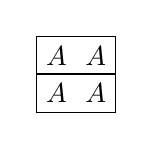
\begin{tikzpicture}[baseline=(O)]
			\matrix (M) [matrix of nodes] {
				$A$ & $A$ \\
				$A$ & $A$ \\
			};
			\coordinate (O) at (M-1-1.south west);
			\draw (M-1-1.north west) rectangle (M-1-2.south east);
			\draw (M-2-1.north west) rectangle (M-2-2.south east);
		\end{tikzpicture} = 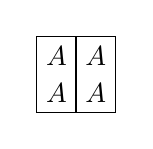
\begin{tikzpicture}[baseline=(O)]
			\matrix (M) [matrix of nodes] {
				$A$ & $A$ \\
				$A$ & $A$ \\
			};
			\coordinate (O) at (M-1-1.south west);
			\draw (M-1-1.north west) rectangle (M-2-1.south east);
			\draw (M-1-2.north west) rectangle (M-2-2.south east);
		\end{tikzpicture} \quad \begin{tabular}{rl}
			横向: & 以 $\mu'$ 相乘 \\
			纵向: & 以 $\mu_A$ 相乘
		\end{tabular}\end{center}
		现在 $\mu' = \mu_A$ 的论证可以图解作
		\begin{center}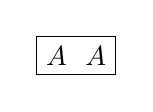
\begin{tikzpicture}[baseline=(O)]
			\matrix (M) [matrix of nodes] {
				$A$ & $A$ \\
			};
			\coordinate (O) at (M-1-1.south west);
			\draw (M-1-1.north west) rectangle (M-1-2.south east);
		\end{tikzpicture}
		$=$ 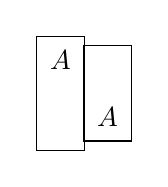
\begin{tikzpicture}[baseline=(O)]
			\matrix (M) [matrix of nodes, every node/.style={anchor=base, minimum width=1.7em, minimum height=1.7em}] {
				$A$ & $\munit$ \\
				$\munit$ & $A$ \\
			};
			\coordinate (O) at (M-1-1.south west);
			\draw (M-1-1.north west) rectangle (M-2-1.south east);
			\draw (M-1-2.north west) rectangle (M-2-2.south east);
		\end{tikzpicture}
		$=$ 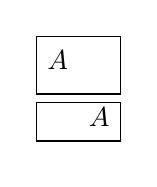
\begin{tikzpicture}[baseline=(O)]
			\matrix (M) [matrix of nodes, every node/.style={anchor=base, minimum width=1.5em, minimum height=1.7em}] {
				$A$ & $\munit$ \\
				$\munit$ & $A$ \\
			};
			\coordinate (O) at (M-1-1.south west);
			\draw (M-1-1.north west) rectangle (M-1-2.south east);
			\draw (M-2-1.north west) rectangle (M-2-2.south east);
		\end{tikzpicture}
		$=$ 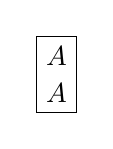
\begin{tikzpicture}[baseline=(O)]
			\matrix (M) [matrix of nodes] {
				$A$ \\
				$A$ \\
			};
			\coordinate (O) at (M-1-1.south west);
			\draw (M-1-1.north west) rectangle (M-2-1.south east);
		\end{tikzpicture}\end{center}
		也请试着翻译为相应的交换图表或等式.
	\end{hint}

	\item 考虑 $\mathcal{A}$ 上的 dg-代数 $A$ (定义 \ref{def:dg-algebra}). 验证当 $A = \munit$ (幺元) 时, 左 $A$-模和右 $A$-模的概念都化约为 $\mathcal{A}$ 上的复形.

	\item 取定交换环 $\Bbbk$. 设 $A$ 为 $\Bbbk\dcate{Mod}$ 上的 dg-代数, $M$ 为复形. 证明赋予 $M$ 左 $A$-模的结构相当于指定 dg-代数的同态 $A \to \End^\bullet(M) := \Hom^\bullet(M, M)$.
	
	\item 设 $\Bbbk$ 为交换环, $R$ 为 $\Bbbk\dcate{Mod}$ 上的 dg-代数. 对于右 $R$-模 $X$ 和左 $R$-模 $Y$, 我们分别将 $R$ 和 $X$, $Y$ 等同于带有直和分解
	\[ R = \bigoplus_n R^n, \quad X = \bigoplus_n X^n, \quad Y = \bigoplus_n Y^n \]
	连同满足 $d^2 = 0$ 的 $1$ 次自同态 $d$ 的 $\Bbbk$-代数和 $\Bbbk$-模. 因此 $X \dotimes{R} Y$ 作为 $\Bbbk$-模已有定义.
	\begin{enumerate}[(i)]
		\item 回忆到 $X \otimes Y = \bigoplus_n (\bigoplus_{p+q=n} X^p \otimes Y^q)$ 既是 $\Bbbk$-模又有复形结构. 对自明的 $\Bbbk$-模同态 $\pi: X \otimes Y \twoheadrightarrow X \dotimes{R} Y$, 验证 $\Ker(\pi)$ 是子复形, 从而 $X \dotimes{R} Y$ 具有典范的复形结构.
		
		\item 证明若 $X$ 为 $(A, R)$-双模, $Y$ 为 $(R, B)$-双模, 其中 $A$ 和 $B$ 也是 dg-代数, 则 $X \dotimes{R} Y$ 自然地成为 $(A, B)$-双模. 以此推广命题 \ref{prop:tensor-Hom-cplx} 的伴随关系至 dg-模的情形; 此处涉及的 $\Hom^\bullet(Y_B, Z_B)$ 和 $\Hom^\bullet({}_A X, {}_A Z)$ 按例 \ref{eg:dg-Hom-cplx} 的方式定义为复形, 但在赋予 $(A, R)$ 和 $(R, B)$-双模结构时须留意符号.
	\end{enumerate}

	\item 选定 $\mathcal{A}$ 上的 dg-代数 $A$. 若 $p > 0 \implies A^p = 0$, 则称 $A$ 是\emph{非正}的. 对于左 (或右) $A$-模 $M$ 和 $n \in \Z$, 以定义 \ref{def:truncation-cplx} 取 $M$ 的截断子复形 $\tau^{\leq n} M$. 证明若 $A$ 非正, 则:
	\begin{enumerate}[(i)]
		\item 每个 $d_M^p: M^p \to M^{p+1}$ 都是 $A^0$-线性的;
		\item 我们有 $A$-模的短正合列 $0 \to \tau^{\leq n} M \to M \to \tilde{\tau}^{\geq n+1} M \to 0$.
	\end{enumerate}
	\index{dg daishu!非正 (non-positive)}
	
	\item 选定 $\mathcal{A}$ 上的 dg-代数 $A$. 回忆到全体左 $A$-模构成 dg-范畴 $A\dcate{dgMod}$ (例 \ref{eg:dg-Hom-cplx}); 注记 \ref{rem:dg-homotopy-cat} 相应地给出同伦范畴 $\mathrm{h}(A\dcate{dgMod})$. 若左 $A$-模 $M$ 作为复形是零调的, 则称 $M$ 零调; 若 $A$-模的态射 $f: M \to N$ 作为复形的态射是拟同构, 则称 $f$ 为拟同构.
	\begin{enumerate}[(i)]
		\item 设 $M$ 为左 $A$-模, 其结构由 $\mathcal{A}$ 中的一族态射 $\alpha_{A, M}^{p, q}: A^p \otimes M^q \to M^{p+q}$ 确定 ($p, q \in \Z$). 说明下式赋予复形 $M[1]$ 左 $A$-模结构:
		\[ \alpha_{A, M[1]}^{p, q} := (-1)^p \alpha_{A, M}^{p, q+1} . \]
		其次, 说明 $M \mapsto M[1]$ 给出从 $A\dcate{dgMod}$ 到自身的 dg-函子.
		\item 对 $A\dcate{dgMod}$ 的任意态射 $f: M \to N$, 说明映射锥 $\Cone(f)$ 具有典范的左 $A$-模结构, 它按先前符号表作
		\[ \alpha_{A, \Cone(f)}^{p, q} = \alpha_{A, M[1]}^{p, q} \oplus \alpha_{A, N}^{p, q}. \]
		\item 循 \S\ref{sec:derived-cat} 的成法, 以映射锥令 $\mathrm{h}(A\dcate{dgMod})$ 成为三角范畴. 其次, 对零调 $A$-模作 Verdier 局部化, 换言之添入拟同构的逆, 以得到导出范畴 $\cate{D}(A\dcate{dgMod})$; 定义相应的 $\cate{D}^{\star}(A\dcate{dgMod})$, 其中 $\star \in \{+, -, \bdd\}$.
		\item 在 $A$ 非正的前提下, 将命题 \ref{prop:derived-full-faithful-subcat} 推广到 $\cate{D}(A\dcate{dgMod})$ 和 $\cate{D}^{\star}(A\dcate{dgMod})$ 情形, $\star \in \{+, -, \bdd\}$.
		\begin{hint}
			使用截断函子.
		\end{hint}
		\item 参照 \S\ref{sec:K-injectives} 来定义何谓 K-内射和 K-投射 $A$-模, 以之描述 $\cate{D}(A\dcate{dgMod})$ 中的态射. 代入 \S\ref{sec:triangulated-functor-localization} 的框架来探讨它们和导出函子的联系.
		\item 对于右 $A$-模 $M$, 说明复形 $M[1]$ 具有如下的右 $A$-模结构: $\alpha_{M[1], A}^{p, q} = \alpha_{M, A}^{p, q+1}$, 而且先前一切性质仍成立.
	\end{enumerate}
	
	\item 设 $\mathcal{C}$ 是 $\Bbbk$ 上的 dg-范畴. 定义 $\mathcal{C}^{\opp}$ 使得 $\Obj\left( \mathcal{C}^{\opp} \right) = \Obj(\mathcal{C})$, 而对任意 $X, Y \in \Obj\left(\mathcal{C}^{\opp}\right)$ 定义复形 $\Hom^\bullet_{\mathcal{C}^{\opp}}(X, Y) := \Hom^\bullet_{\mathcal{C}}(Y, X)$, 其上的合成运算定为
	\begin{align*}
		\Hom^p_{\mathcal{C}^{\opp}}(Y, Z) \dotimes{\Bbbk} \Hom^q_{\mathcal{C}^{\opp}}(X, Y) & \to \Hom^{p+q}_{\mathcal{C}^{\opp}}(X, Z) \quad p, q \in \Z \\
		f \otimes g & \mapsto (-1)^{pq} \underbracket{f \circ g}_{\Hom^\bullet_{\mathcal{C}}\;\text{的运算}}.
	\end{align*}
	验证这确实给出 dg-范畴 $\mathcal{C}^{\opp}$, 称为 $\mathcal{C}$ 的相反 dg-范畴.
	
	\item 选定交换环 $\Bbbk$ 和 $\Bbbk\dcate{Mod}$ 上的 dg-代数 $R$, 右 $R$-模和左 $R$-模 $Y$. 证明先前介绍的
	\[ X \dotimes{R} (\cdot): R\dcate{dgMod} \to \cate{C}(\Bbbk), \quad (\cdot) \dotimes{R} Y: \cated{dgMod}R \to \cate{C}(\Bbbk) \]
	自然地升级为 dg-函子. 对于 $X$ 或 $Y$ 另带双模结构的情形勾勒相应的结果.
	
	\begin{hint}
		关键在于定义 $\Hom$ 复形之间的态射. 对于 $X \dotimes{R} (\cdot)$, 设 $M$ 和 $N$ 为左 $R$-模, 则 Koszul 符号律要求将 $f \in \Hom^n_R(M, N)$ 的像 $\identity_X \otimes f \in \Hom^n(X \dotimes{R} M, X \dotimes{R} N)$ 定义为
		\[ (\identity_X \otimes f)(x \otimes m) = (-1)^{pn} x \otimes f(m), \quad x \in X^p, \; m \in M^q. \]
		须验证 $\identity_X \otimes d_{\Hom^\bullet}(f) = d_{\Hom^\bullet}(\identity_X \otimes f)$.
		
		至于 $(\cdot) \dotimes{R} Y$ 的情形则比较简单, 取 $(f \otimes \identity_Y)(m \otimes y) = f(m) \otimes y$ 即可.
	\end{hint}
	
	\item 设 $\mathcal{C}$ 为交换环 $\Bbbk$ 上的 dg-范畴, $M \in \Obj(\mathcal{C})$.
	\begin{enumerate}[(i)]
		\item 将 $\Hom^\bullet(M, \cdot): \mathcal{C} \to \cate{C}(\Bbbk)$ 升级为 dg-函子.
		
		\begin{hint}
			设 $X, Y \in \Obj(\mathcal{C})$ 而 $f \in \Hom^n(X, Y)$. 命 $\mathcal{H}_X = \Hom^\bullet(M, X)$, 则 $f$ 的像应当取为
			\[ \left[ f_*: g \xmapsto{n\;\text{次态射}} fg \right] \in \Hom^n(\mathcal{H}_X, \mathcal{H}_Y). \]
			代入 $\Hom$ 复形的定义来验证 $(d_{\Hom^\bullet(X, Y)} f)_* = d_{\Hom^\bullet(\mathcal{H}_X, \mathcal{H}_Y)}(f_*)$.
		\end{hint}
		\item 将 $\Hom^\bullet(\cdot, M): \mathcal{C} \to \cate{C}(\Bbbk)^{\opp}$ 升级为 dg-函子.
		
		\begin{hint}
			命 $\mathcal{K}_X = \Hom^\bullet(X, M)$, 则 Koszul 符号律要求将 $f \in \Hom^n(X, Y)$ 的像取为
			\[ \left[\begin{array}{c}
				f^*: g \xmapsto{n\;\text{次态射}} (-1)^{np} gf \\
				\forall p \in \Z , \; \forall\; g \in \Hom^p(Y, M)
			\end{array}\right] \in \Hom^n(\mathcal{K}_Y, \mathcal{K}_X). \]
			细心地验证
			\begin{compactitem}
				\item $(d_{\Hom^\bullet(X, Y)} f)^* = d_{\Hom^\bullet(\mathcal{K}_Y, \mathcal{K}_X)}(f^*)$,
				\item $(fh)^*$ 等于 $h^*$ 和 $f^*$ 在 $\Hom^\bullet_{\cate{C}(\Bbbk)}$ 中的合成.
			\end{compactitem}
		\end{hint}
	\end{enumerate}
	
	\item 证明 \S\ref{sec:closed-monoidal} 对闭幺半范畴定义的典范态射 $[Y, Z] \otimes [X, Y] \to [X, Z]$ 和 $\munit \to [X, X]$ 满足结合律和幺元的性质, 从而使闭幺半范畴相对于内 $\Hom$ 是自充实的.
	\begin{hint}
		直接验证, 或者参考 \cite[Section 1.6]{Kel05}.
	\end{hint}

	\item 考虑交换环 $\Bbbk$ 上的多项式代数 $\Bbbk[t]$. 取 $\Delta, \epsilon, S$ 分别为
	\[ \Delta(t^n) = \sum_{k=0}^n \binom{n}{k} t^k \otimes t^{n-k}, \quad \epsilon(t^n) = \begin{cases}
		1, & n = 0 \\
		0, & n \neq 0
	\end{cases}, \quad
	S(t^n) = (-1)^n t^n, \]
	其中 $n \in \Z_{\geq 0}$. 验证这给出交换而且余交换的 Hopf $\Bbbk$-代数.
	
	\item 若交换环上的 Hopf 代数 $A$ 的理想 $I$ 满足 $\Delta(I) \subset I \otimes A + A \otimes I$, $\epsilon(I) = 0$ 和 $S(I) \subset I$, 则称之为 Hopf 理想. 说明对 Hopf 理想取商给出 Hopf 代数 $A/I$.
	
	\item 设 $\Bbbk$ 是交换环而 $V$ 是 $\Bbbk$-模. 对张量代数 $T(V)$ (见 \cite[定义 7.5.1]{Li1}) 可以定义 $\Bbbk$-代数的同态 $\Delta: T(V) \to T(V) \otimes T(V)$ 和 $\epsilon: T(V) \to \Bbbk$, 使得对所有 $v \in V$ 都有
	\begin{gather*}
		\Delta(v) = v \otimes 1 + 1 \otimes v, \quad \epsilon(v) = 0;
	\end{gather*}
	此处以平凡辫结构 $x \otimes y \mapsto y \otimes x$ 赋予 $T(V) \otimes T(V)$ 代数的结构.
	\begin{enumerate}[(i)]
		\item 验证 $T(V)$ 对此成为双代数.
		\item 说明如何定义 $\Bbbk$-模自同构 $S: T(V) \to T(V)$ 使得 $S(v) = -v$, 并且使 $S$ 是双代数的反自同构 (命题 \ref{prop:Hopf-antiautomorphism}); 更具体地说,
		\[ S(v_1 \cdots v_n) = (-1)^n v_n \cdots v_1, \quad n \in \Z_{\geq 0}, \quad v_1, \ldots, v_n \in V. \]
		验证 $T(V)$ 依此成为 Hopf 代数.
		\item 说明对称代数 $\Sym(V)$ 也有类似性质, 它事实上是 $T(V)$ 对一个 Hopf 理想的商.
		\item 处理外代数 $\bigwedge(V)$ 的版本, 但 $\bigwedge(V) \otimes \bigwedge(V)$ 上的乘法结构应该用 Koszul 辫结构 \eqref{eqn:Koszul-braiding} 来定义 (在该处取 $\epsilon(a) = a \bmod\; 2$), 使得齐次元 $x, y, z, w \in \bigwedge(V)$ 满足 $(x \otimes y)(z \otimes w) = (-1)^{\deg y \deg z} xz \otimes yw$. 这可以确保 $(1 \otimes v + v \otimes 1)^2$ 对所有 $v \in V$ 都被映为 $\bigwedge(V) \otimes \bigwedge(V)$ 的零元.
	\end{enumerate}
	
	\item (E.\ Taft) 设 $q$ 是域 $\Bbbk$ 的 $n$ 次单位原根, $n \geq 2$. 考虑由生成元 $g$, $x$ 和关系
	\[ g^n = 1, \quad x^n = 0, \quad gxg^{-1} = qx \]
	确定的 $\Bbbk$-代数 $H$. 说明可以定义 $\Delta: H \to H \dotimes{\Bbbk} H$ 和 $\epsilon: H \to \Bbbk$, 满足
	\begin{gather*}
		\Delta(g) = g \otimes g, \quad \Delta(x) = 1 \otimes x + x \otimes g, \\
		\epsilon(g) = 1, \quad \epsilon(x) = 0,
	\end{gather*}
	而且这使 $H$ 成为 Hopf $\Bbbk$-代数, 带有对极
	\[ S: H \to H, \quad S(g) = g^{-1}, \quad S(x) = -g^{-1}x. \]
	
	说明 $H$ 既非交换亦非余交换. 当 $n=2$ 时, 对应的 Hopf 代数也称为 Sweedler 的 Hopf 代数.

	\item 设 $(A, \Delta, \epsilon)$ 为交换环 $\Bbbk$ 上的余代数. 若 $x \in A$ 满足 $\Delta(x) = 1 \otimes x + x \otimes 1$, 则称 $x$ 是\emph{本原}的.
	\begin{enumerate}[(i)]
		\item 证明对所有本原的 $x$ 皆有 $\epsilon(x) = 0$.
		\item 设 $(A, \mu, \eta, \Delta, \epsilon)$ 为双代数, 将 $\mu$ 表作乘法 ($xy = \mu(x \otimes y)$). 证明若 $x, y \in A$ 是本原元素, 则 $xy - yx$ 亦然.
		\item 仍然设 $A$ 为双代数, 设 $x_1, \ldots, x_n \in A$ 为本原元素, 记以 $x_1, \ldots, x_n$ 为基的自由 $\Bbbk$-模为 $V$. 由此得到 $\Bbbk$-代数同态 $\phi: T(V) \to A$. 证明 $\phi$ 也是双代数的同态.
	\end{enumerate}

	\item 设 $(A, \Delta, \epsilon)$ 是交换环 $\Bbbk$ 上的余代数, $A \neq \{0\}$, 而且它作为 $\Bbbk$-模是无挠的. 满足 $\Delta(x) = x \otimes x$ 的非零元 $x \in A$ 称为\emph{类群}的. 全体类群元素所成集合记为 $\mathcal{G}(A)$.
	\begin{enumerate}[(i)]
		\item 证明 $x \in \mathcal{G}(A)$ 蕴涵 $\epsilon(x) = 1$.
		\item 证明若 $(A, \mu, \eta, \Delta, \epsilon)$ 是双代数, 则 $\mathcal{G}(A)$ 对 $A$ 的乘法 $\mu$ 成为幺半群, 以 $1_A := \eta(1)$ 为幺元.
		\item 对于幺半群 $M$ 及对应的双代数 $\Bbbk[M]$ (例 \ref{eg:monoid-bialgebra}), 证明 $\mathcal{G}(\Bbbk[M]) = M$.
		\item 设 $A$ 是以 $S$ 为对极的 Hopf 代数, 证明 $\mathcal{G}(A)$ 是群, $x \in \mathcal{G}(A)$ 的逆是 $S(x)$.
	\end{enumerate}
	
	\item 设 $(A, \Delta, \epsilon)$ 是域 $\Bbbk$ 上的余代数, $A \neq \{0\}$. 证明 $\mathcal{G}(A)$ 是 $A$ 的线性无关子集.
	
	\begin{hint}
		设若不然, 取其中最短的非平凡线性关系, 不妨写作 $x_1 = \sum_{i=2}^n a_i x_i$, 其中 $x_1, \ldots, x_n \in \mathcal{G}(A)$ 两两相异, $a_i \in \Bbbk$. 于是 $x_2, \ldots, x_n$ 线性无关, 而 $x_1 \otimes x_1 = \sum_{i=2}^n a_i x_i \otimes x_i$.
	\end{hint}

	\item 命 $\cate{TopCMon}$ 为交换拓扑幺半群范畴, $\cate{Top}_\bullet$ 为带基点拓扑空间范畴, $U: \cate{TopCMon} \to \cate{Top}_\bullet$ 为忘却函子 (基点对应幺元). 试构造 $U$ 的左伴随函子 $\Sym: \cate{Top}_\bullet \to \cate{TopCMon}$. 对应于带基点拓扑空间 $(X, x)$ 的 $\Sym(X, x)$ 又称为 $(X, x)$ 的无穷对称积, 试解释这一术语. 代数拓扑学中的 Dold--Thom 定理便是基于这一构造.
	
	% Reference: Deligne, Categories tannakiennes, 4.5 Proposition.
	\item 设 $(A, B)$-双模 $P$ 作为右 $B$-模是有限生成投射模, 而且 $(\cdot) \dotimes{A} P$ 是忠实正合函子. 证明右 $A$-模 $N$ 是有限展示的 (例 \ref{eg:Mod-cpt}) 当且仅当 $N \dotimes{A} P$ 是有限展示右 $B$-模. 这是命题 \ref{prop:Morita-comonad-ft} 的补充.
	
	\item 考虑交换环 $\Bbbk$ 和 $\Bbbk$-代数的同态 $f: A \to B$. 我们有伴随对
	\[\begin{tikzcd}
		\mathcal{F}_{B|A}: \cated{Mod}B \arrow[shift left, r] & \cated{Mod}A: \Hom_A(B, \cdot), \arrow[shift left, l]
	\end{tikzcd}\]
	其中对所有右 $A$-模 $N$, 以 $(\phi b)(x) = \phi(bx)$ 赋予 $\Hom_A(B, N)$ 右 $B$-模结构. 详言之,
	\begin{compactitem}
		\item 单位态射 $M \to \Hom_A(B, M)$ 映 $m$ 为 $[b \mapsto mb]$,
		\item 余单位态射 $\Hom_A(B, N) \to N$ 映 $\phi$ 为 $\phi(1)$;
	\end{compactitem}
	可见 \cite[推论 6.6.8]{Li1}. 作为例 \ref{eg:comonad-change-ring} 的补充, 请明确它所对应的单子和余单子.

	\item 设 $R$ 是交换环. 记 $R\dcate{Alg}$ 为 $R$-代数所成范畴. 考虑伴随对
	$\begin{tikzcd}
		T(\cdot): R\dcate{Mod} \arrow[shift left, r] & R\dcate{Alg}: U \arrow[shift left, l]
	\end{tikzcd}$,
	其中 $T(\cdot)$ 是取张量代数, $U$ 是忘却.
	\begin{enumerate}[(i)]
		\item 直接证明 $R\dcate{Mod}$ 上对应的单子作用下的模是 $R$-代数, 从而说明伴随对是单子的.
		\item 以 $\Sym(\cdot)$ 和 $\bigwedge(\cdot)$ 代替 $T(\cdot)$, 陈述并证明相应的结果; 可参考 \cite[\S 7.6]{Li1}.
	\end{enumerate}

	\item 试补全命题 \ref{prop:Comod-abelian} 的论证, 并且进一步证明以下的强化版本: 设 $C$ 是 $(B, B)\dcate{Mod}$ 中的余代数, 证明:
	\begin{enumerate}[(i)]
		\item 忘却函子 $U: \cated{Comod}C \to \cated{Mod}B$ 有右伴随;
		
		\begin{hint}
			记 $C$ 的余乘法为 $\Delta$, 余幺元为 $\epsilon$. 对右 $B$-模 $N$, 以 $\identity_N \otimes \Delta$ 将 $N \dotimes{B} C$ 作成右 $C$-余模. 对所有右 $C$-余模 $M$, 须验证
			\[\begin{tikzcd}[row sep=tiny]
				\Hom_{\cated{Mod}B}(M, N) \arrow[shift left, r] & \Hom_{\cated{Comod}C}\left(M, N \dotimes{B} C\right) \arrow[shift left, l] \\
				\varphi \arrow[mapsto, r] & (\varphi \otimes \identity_C) \rho \\
				(\identity_N \otimes \epsilon) \psi & \psi \arrow[mapsto, l]
			\end{tikzcd}\]
			互为逆, 其中 $\rho: M \to M \dotimes{B} C$ 确定 $M$ 的余模结构.
		\end{hint}
		\item 忘却函子 $U$ 生所有小 $\varinjlim$, 因此 $\cated{Comod}C$ 余完备;
		\item 范畴 $\cated{Comod}C$ 有余生成元 (定义 \ref{def:generators});
		
		\begin{hint}
			取 Grothendieck 范畴 $\cated{Mod}B$ 的余生成元, 然后取它对
			$U$ 的右伴随函子的像.
		\end{hint}
		\item 证明若 $\cated{Comod}C$ 是 Abel 范畴, 而且 $U$ 是正合函子, 则 $C$ 作为左 $B$-模是平坦的.
		
		\begin{hint}
			设 $g: M \to N$ 是右 $B$-模的单同态. 由 $U$ 正合与右伴随保核这一事实来说明 $g \otimes \identity_C: M \dotimes{B} C \to N \dotimes{B} C$ 仍是单射.
		\end{hint}
	\end{enumerate}

	\item 如上题, 继续设 $C$ 是 $(B, B)\dcate{Mod}$ 中的余代数, 而 $M$ 是右 $C$-余模. 证明 $M$ 的任意 $B$-商模 $M''$ (或 $B$-子模 $M'$) 若具有余模结构, 使得 $M \twoheadrightarrow M''$ (或 $M' \hookrightarrow M$) 是余模同态, 则这样的余模结构是唯一的, 前提是在子模情形须假设 $C$ 作为左 $B$-模平坦.

	\item 依照 \S\ref{sec:descent-Galois} 末尾的解释, 按以下步骤给出 Galois 下降定理 \ref{prop:Galois-descent} 的直接证明. 沿用该处符号, 设 $M \in \Obj(\cate{Vect}^{\Gamma, \infty}(L))$, 以 \eqref{eqn:Galois-descent-iotaM} 定义典范映射 $\iota_M$.
	\begin{enumerate}[(i)]
		\item 设 $M'$ 是 $L \dotimes{K} (M^\Gamma)$ 的 $\Gamma$-不变子空间 (亦即 $\Gamma M' \subset M'$). 证明若 $M' \cap (1 \otimes M^\Gamma) = \{0\}$, 则 $M' = \{0\}$.
		
		\begin{hint}
			选定 $M^\Gamma$ 的基 $(y_i)_{i \in I}$. 若 $M' \neq \{0\}$, 选其中最短的非零表达式 $\sum_{i \in I} \ell_i \otimes y_i$ (有限和), 适当调整后可以假设它形如
			\[ m' = 1 \otimes y_{i_0} + \ell_1 \otimes y_{i_1} + \cdots, \quad \ell_1 \notin K. \]
			取 $\sigma \in \Gamma$ 使得 $\sigma(\ell_1) \neq \ell_1$, 考虑 $m' - \sigma(m')$ 以得到矛盾.
		\end{hint}
		\item 证明 $\iota_M: L \dotimes{K} (M^\Gamma) \to M$ 是单射.
		\begin{hint}
			考虑 $M' := \Ker(\iota_M)$.
		\end{hint}
		
		\item 证明 $\iota_M$ 是满射.
		
		\begin{hint}
			考虑 $L|K$ 的有限 Galois 子扩张 $E|K$. 取 $E$ 作为 $K$-向量空间的基 $a_1, \ldots, a_n$, 枚举 $\Gal(L|E)$ 的元素 $\identity = \sigma_1, \ldots, \sigma_n$. 应用域论知识可知 $(\sigma_i(a_j))_{1 \leq i, j \leq n}$ 是 $E$ 上的可逆矩阵, 其逆记为 $(b_{ij})_{1 \leq i, j \leq n}$. 对 $m \in M^{\Gal(L|E)}$ 推导
			\[ m = \sum_{i=1}^n b_{i1} \sum_{j=1}^n \sigma_j(a_i m) \; \in \Image(\iota_M). \] 
		\end{hint}
		
		\item 以上述结果说明 \eqref{eqn:Galois-descent-adjunction} 是伴随等价, 从而给出定理 \ref{prop:Galois-descent} 的一个直接证明.
	\end{enumerate}
	
	\item 设 $G$ 为群, $L|K$ 为域的 Galois 扩张. 记系数在域 $K$ (或 $L$) 上的 $G$-模范畴为 $G\dcate{Mod}$ (或 $G\dcate{Mod}_L$); 参阅定义 \ref{def:G-mod}. 运用 \S\S\ref{sec:descent-Galois}---\ref{sec:Galois-H1} 的 Galois 下降方法, 以 $G\dcate{Mod}_L$ 的对象连同合适的 $\Gal(L|K)$-作用来描述 $G\dcate{Mod}$.
	
	\item 沿用 \S\ref{sec:Galois-H1} 的符号. 设 $c \in Z^1(\Gamma, G(\mathbf{t}_{0, L}))$, 回忆定理 \ref{prop:Galois-H1} 的证明, 可见它通过 Galois 下降定义了 $K$-向量空间 $W$ 和其上的资料 $\mathbf{t}$, 以及 $h: \mathbf{t}_{0, L} \rightiso \mathbf{t}_L$.
	\begin{enumerate}[(i)]
		\item 说明 $g \mapsto h^{-1} g h$ 给出群同构 $\nu: G(\mathbf{t}_L) \rightiso G(\mathbf{t}_{0, L})$; 说明 $f \xmapsto{\sigma \in \Gamma} c(\sigma) ({}^\sigma f) c(\sigma)^{-1}$ 赋予 $G(\mathbf{t}_{0, L})$ 新的 $\Gamma$-作用, 另记此结构为 ${}^c G(\mathbf{t}_{0, L})$, 而且 $\nu: G(\mathbf{t}_L) \rightiso {}^c G(\mathbf{t}_{0, L})$ 保持 $\Gamma$-作用.
		\item 说明下式给出良定义的映射
		\begin{align*}
			Z^1(\Gamma, G(\mathbf{t}_L)) & \to Z^1(\Gamma, G(\mathbf{t}_{0, L})) \\
			\tilde{c} & \mapsto \left[\sigma \mapsto \nu(\tilde{c}(\sigma)) c(\sigma) \right],
		\end{align*}
		它诱导双射 $\Hm^1(\Gamma, G(\mathbf{t}_L)) \to \Hm^1(\Gamma, G(\mathbf{t}_{0, L}))$, 映基点为 $[c]$.
		\begin{hint}
			对照\CHref{sec:group-coh}习题中关于``扭曲''的构造.
		\end{hint}
		\item 说明相对于定理 \ref{prop:Galois-H1}, 此双射对应于等式 $\mathscr{T}(\mathbf{t}) = \mathscr{T}(\mathbf{t}_0)$.
	\end{enumerate}
	
	\item 选定满足 $\mathrm{char}(K) \neq 2$ 的域 $K$. 有限维 $K$-向量空间 $V$ 上的非退化对称双线性型 $q: V \times V \to K$ 简称非退化二次型; 在正交群 $\mathrm{O}(q) = \mathrm{O}(V, q)$ 中, 记 $\det = 1$ 截出的子群为 $\SO(q) = \SO(V, q)$. 对任意 Galois 扩张 $L|K$, 我们有非退化二次型 $(V_L, q_L)$ 和对应的群, 其上都有 $\Gamma := \Gal(L|K)$ 的光滑作用.
	\begin{enumerate}[(i)]
		\item 记 $\mu_2 := \{\pm 1\} \subset K^\times$. 说明 $\mathrm{O}(q)/\SO(q) \simeq \mu_2$; 对于 $\mathrm{O}(q_L)/\SO(q_L)$ 的版本, 说明同构和 $\Gamma$-作用有何关系.
		\item 基于 \S\ref{sec:Galois-H1} 的工具, 说明 $\Hm^1(\Gamma, \mathrm{O}(q_L))$ 的元素一一对应于 $K$ 上满足 $\dim V' = \dim V$ 的非退化二次型 $(V', q')$ 的同构类, 基点对应 $(V, q)$.
		\item 代入定理 \ref{prop:nonabelian-long} 推导带基点集的正合列
		\[ \mathrm{O}(q) \xrightarrow{\det} \mu_2 \to \Hm^1(\Gamma, \SO(q_L)) \xrightarrow{\varphi} \Hm^1(\Gamma, \mathrm{O}(q_L)) \xrightarrow{\psi} \Hm^1(\Gamma, \mu_2). \]
		试说明 $\varphi$ 是单射.
		\begin{hint}
			由 $\det$ 满只能说明 $\varphi^{-1}(\text{基点}) = \{\text{基点}\}$; 为了说明单性, 须变化 $(V, q)$, 并应用上一道习题的扭曲技巧.
		\end{hint}
		\item 说明 $\Hm^1(\Gamma, \mu_2) \simeq K^\times / K^{\times, 2}$. 说明 $\psi$ 等同于映射
		\[ \left[ (V', q'):\; \text{非退化二次型} \right] \mapsto \mathrm{disc}(q') / \mathrm{disc}(q), \]
		其中我们任取 $V'$ 的基, 将 $q'$ 等同于一个对称矩阵, 然后定义
		\[ \mathrm{disc}(q') := (-1)^n \det(q') \bmod K^{\times 2}, \quad \dim V = 2n \;\text{或}\; 2n+1. \]
		\item 说明 $\Hm^1(\Gamma, \SO(q_L))$ 的元素一一对应于 $K$ 上满足 $\dim V' = \dim V$ 和 $\mathrm{disc}(q') = \mathrm{disc}(q)$ 的非退化二次型 $(V', q')$ 的同构类, 基点对应到 $(V, q)$.
	\end{enumerate}
\end{Exercises}

	% LaTeX source for book ``代数学方法'' in Chinese
% Copyright 2024  李文威 (Wen-Wei Li).
% Permission is granted to copy, distribute and/or modify this
% document under the terms of the Creative Commons
% Attribution 4.0 International (CC BY 4.0)
% http://creativecommons.org/licenses/by/4.0/

% To be included
\chapter{单纯形方法}\label{sec:simplicial}
命 $\simpDelta$ 为非零有限序数范畴. 范畴 $\mathcal{C}$ 中的单纯形对象按定义是从 $\simpDelta^{\opp}$ 到 $\mathcal{C}$ 的函子 $X$, 它们也可以等价地描述为一列对象 $X_0, X_1, \ldots$ 及其间的态射 $d_i: X_n \to X_{n-1}$ (面) 和 $s_j: X_n \to X_{n+1}$ (退化), $0 \leq i, j \leq n$, 服从于一族等式 \eqref{eqn:simplicial-identity}; 这些函子构成范畴 $\cate{s}\mathcal{C}$. 对于 $\mathcal{C} = \cate{Set}$ 的特例, 它们也称为单纯形集. 相关的基本理论是 \S\S\ref{sec:simplicial-method}---\ref{sec:simplicial-set} 的内容. 命 $\cate{FinOrd}$ 为有限序数范畴, 若单纯形对象 $X$ 作为函子延拓为 $\cate{FinOrd} \to \mathcal{C}$, 则称之为增广单纯形对象, 这相当于在资料 $(X_n, d_i, s_j)_{n, i, j}$ 中添入 $-1$ 次项 $X_{-1}$.

单纯形集源于拓扑学, 想法是将空间剖分为单纯形的黏贴; 单纯形 (点, 线段, 三角形, 四面体...) 的直观图像是
\begin{center}\begin{tabular}{ccccc}
	$0$ 维 & $1$ 维 & $2$ 维 & $3$ 维 & $\cdots$ \\
	
\begin{tikzpicture}[baseline=(P)] \fill[black] (0.5, 0.5) circle[radius=0.07]; \coordinate (P) at (0, 0.5); \end{tikzpicture} &
	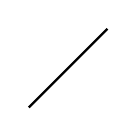
\begin{tikzpicture}[baseline=(P)] \draw[thick] (0,0) -- (1,1); \coordinate (P) at (0.5, 0.5); \end{tikzpicture} &
	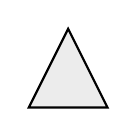
\begin{tikzpicture}[baseline=(P)] \filldraw[thick, fill=gray!15] (0,1) -- (-0.5, 0) -- (0.5, 0) --cycle; \coordinate (P) at (0, 0.5); \end{tikzpicture} &
	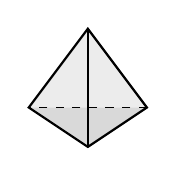
\begin{tikzpicture}[baseline=(P)]
		\fill[color=gray!15] (0, 1) -- (0.75, 0) -- (0, -0.5) -- (-0.75, 0) --cycle;
		\fill[color=gray!30] (0.75, 0) -- (0, -0.5) -- (-0.75, 0) --cycle;
		\draw[dashed] (0.75, 0) -- (-0.75, 0);
		\draw[thick] (0, 1) -- (0.75, 0) -- (0, -0.5) -- (-0.75, 0) --cycle;
		\draw[thick] (0, 1) -- (0, -0.5);
		\coordinate (P) at (0, 0.3);
	\end{tikzpicture} &
	$\cdots$
\end{tabular}\end{center}
依此对空间的同调和同伦等问题获取具体的, 或谓组合的理解. 此处采取的严格表述由 S.\ Eilenberg 和 J.\ A.\ Zilber 在 1950 年引入. 单纯形集的语言具有广泛的解释能力, 不限于经典的拓扑问题: 举例来说, 它能通过称为``脉''的构造来描述范畴, 详见 \S\ref{sec:nerves} 的介绍; 既然范畴论探讨图表中的对象 (表现为零维的点), 态射 (表现为一维的箭头) 和交换性 (关乎三角或方块等二维组件), 范畴和空间能统合于同一种数学结构之下并非意外.

在介绍脉和分类空间作为单纯形集的基本实例之后, \S\ref{sec:geom-realization} 回归直观, 定义单纯形集 $X$ 的几何实现 $|X|$; 定理 \ref{prop:geom-Sing-adjunction} 说明它和拓扑学家所熟悉的奇异集函子 $\mathrm{Sing}$ 一道构成伴随对
\[\begin{tikzcd}
	{|\cdot|}: \cate{sSet} \arrow[shift left, r] & \cate{Top} : \mathrm{Sing}. \arrow[shift left, l]
\end{tikzcd}\]
如以同伦论所常用的紧生成 Hausdorff 空间范畴 $\cate{CGHaus}$ 代替 $\cate{Top}$, 则几何实现还满足 $|X \times Y| \simeq |X| \times |Y|$, 左式的乘积是对两个单纯形集逐项取积; 证明关乎乘积的剖分, 其中一些组合学细节不尽平凡, 由于本书并非拓扑教材, 细节不深究.

相对于本书的主题, 更重要的是考虑 Abel 范畴 $\mathcal{A}$ 中的单纯形对象, 此时 $\cate{s}\mathcal{A}$ 也是 Abel 范畴; 例如单纯形 Abel 群构成 Abel 范畴 $\cate{sAb}$. 这方面的根本结果是 \S\ref{sec:Dold-Kan} 探讨的 Dold--Kan 对应 (定理 \ref{prop:Dold-Kan}), 它对 Abel 范畴 $\mathcal{A}$ 给出一对伴随等价
\[\begin{tikzcd}
	\Gamma: \cate{s}\mathcal{A} \arrow[shift left, r] & \cate{Ch}_{\geq 0}(\mathcal{A}): \mathrm{N}, \arrow[shift left, l]
\end{tikzcd}\]
其中 $\cate{Ch}_{\geq 0}(\mathcal{A})$ 代表 $\mathcal{A}$ 上的非负次链复形所成之 Abel 范畴. 函子 $\mathrm{N}$ 映单纯形对象 $X$ 为相应的正规化链复形 $\mathrm{N}X$; 更精确地说, 定义 $X \in \Obj(\cate{s}\mathcal{A})$ 的非正规化链复形为
\[ \mathrm{C}X := \left( X_n, \partial_n\right)_{n \geq 0}, \quad \partial_n := \sum_{i=0}^n (-1)^n d_i : X_n \to X_{n-1}, \]
则 $\mathrm{N}X$ 既可以按 $(\mathrm{N}X)_n := \bigcap_{i=1}^n \Ker(d_i)$ 取为 $\mathrm{C}X$ 的子链复形, 也可以理解为 $\mathrm{C}X$ 对退化部分的商, 两者之间的同构是命题 \ref{prop:Dold-Kan-v} 的内容; 事实上, 定理 \ref{prop:Dold-Kan-N-C} 说明嵌入态射 $u: \mathrm{N}X \to \mathrm{C}X$ 是链复形之间的拟同构.

Dold--Kan 对应使得单纯形理论不只在历史上, 而且在思想和技术两方面都成为同调代数的根源. 单纯形方法能够解释并升级复形或链复形上的基本操作, 例如同伦或可缩性质都有单纯形的版本, 从而获取拓扑诠释, 这部分讨论见诸 \S\ref{sec:homology-computation}.

另一种应用是搭配 \S\ref{sec:Beck} 的单子理论, 由此可以典范地将范畴中的对象扩充为相应的增广单纯形对象或增广余单纯形对象; 鉴于它们和 Hochschild 同调中的``加杠''操作有关, 这些技术统称为杠构造, 是 \S\ref{sec:bar-resolution} 的主题. 通过 Dold--Kan 对应和一些关于可缩性的观察, 杠构造解释了 Hochschild 理论 (见 \S\ref{sec:HH}) 和群上同调理论 (见 \S\ref{sec:G-mod}) 中的种种标准解消, 说明它们出于更高阶的奇思妙想. 习题包含关于杠构造的其他延伸内容.

按照定义, \S\ref{sec:bisimplicial} 讨论的双单纯形对象无非是函子 $\simpDelta^{\opp} \times \simpDelta^{\opp} \to \mathcal{C}$, 它们构成范畴 $\cate{s}^2 \mathcal{C}$. 对于取 $\mathcal{A}$ 为 Abel 范畴的情形, 与 $\cate{s}^2 \mathcal{A}$ 直接相关的 Eilenberg--Zilber 定理 \ref{prop:Eilenberg-Zilber} 是代数拓扑学中的基本构造; 纯粹从范畴论观点看, 在 $\mathcal{A}$ 为幺半范畴的前提下 (例如 $\mathcal{A} = \cate{Ab}$), 它为函子 $\mathrm{N}: \cate{s}\mathcal{A} \to \cate{Ch}_{\geq 0}(\mathcal{A})$ 提供了双向的典范幺半结构. 然而双单纯形对象的应用不止于此.

本章最后的 \S\ref{sec:closed-simplicial} 和 \S\ref{sec:mapping-cone-revisited} 分别探讨单纯形集的 $\Hom$ 对象和映射锥. 它们一方面对应到拓扑直观中的映射空间和锥, 另一方面又在 Abel 群情形通过 Dold--Kan 对应给出熟悉的 $\Hom$ 链复形和映射锥. 复形或链复形上的相应构造因此获得了明白的解释, 而拓扑学家对这一切如数家珍.

\begin{wenxintishi}
	本章的 \S\S\ref{sec:simplicial-method}---\ref{sec:geom-realization} 构成单纯形方法的主干, \S\S\ref{sec:Dold-Kan}---\ref{sec:bar-resolution} 和链复形直接相关, 而 \S\S\ref{sec:bisimplicial}---\ref{sec:mapping-cone-revisited} 尽管和本书先前的内容声气相通, 其属性则接近延伸内容. 相对于本书其他各章, 单纯形方法并非逻辑必需品, 然而其中的思想与技术属于数学工作者的基本素养, 更是踏入高阶代数的基础. 关于单纯形对象的一些论证有时涉及琐碎的验证 (如 \S\ref{sec:Dold-Kan}), 这是定义使然, 请读者酌情选择.
\end{wenxintishi}

\section{单纯形对象}\label{sec:simplicial-method}
我们在注记 \ref{rem:walking-algebra} 回顾了何谓偏序集之间的保序映射, 并且由之定义了有限序数范畴 $\cate{FinOrd}$. 本章聚焦于非零序数构成的全子范畴 $\simpDelta$.

\begin{definition}
	\index[sym1]{Delta-simp@$\simpDelta$}
	\index[sym1]{[n]}
	令 $\simpDelta$ 为所有有限非零序数及其间的保序映射构成的范畴. 换言之, 它的对象是全序集 $[n] := \{0, \ldots, n \}$, 其中 $n \in \Z_{\geq 0}$, 而态射是保序映射.
\end{definition}

请注意: 不应混淆 $[n]$ 与 $\mathbf{n}$, 后者在本书中代表全序集 $\{0, \ldots, n-1 \}$ 或相应的范畴.

范畴 $\simpDelta$ 中的任意态射 $[l] \to [n]$ 都能唯一地分解为保序满射和保序单射的合成
\[ [l] \twoheadrightarrow [m] \hookrightarrow [n], \quad n \geq m \leq l, \]
而如上的单射 (或满射) 又可以拆成片段, 使得每步恰好遗漏一个元素 (或恰好简并两个元素); 换言之, 所有态射都能分解为下述两类态射的合成.
\begin{center}\begin{tabular}{|c|l|l|l|} \hline
	余面 & $\mathrm{d}^i = \mathrm{d}^{n, i}: [n-1] \hookrightarrow [n]$ & $0 \leq i \leq n$ & 仅遗漏 $i \in [n]$ 的保序单射 \\ \hline
	余退化 & $\mathrm{s}^j = \mathrm{s}^{n, j}: [n+1] \twoheadrightarrow [n]$ & $0 \leq j \leq n$ & 取两次 $j \in [n]$ 的保序满射 \\ \hline
\end{tabular}\end{center}

一个保序单射 (或满射) 可按多种方式分解为余面 (或余退化), 取决于遗漏 (或简并) 元素的次序. 以下的\emph{余单纯形等式}的验证毫无困难:
\begin{equation}\label{eqn:cosimplicial-identity}\begin{array}{ll}
	\mathrm{d}^j \mathrm{d}^i = \mathrm{d}^i \mathrm{d}^{j-1}, & i < j, \\
	\mathrm{s}^j \mathrm{d}^i = \mathrm{d}^i \mathrm{s}^{j-1} & i < j, \\
	\mathrm{s}^j \mathrm{d}^j = \identity = \mathrm{s}^j \mathrm{d}^{j+1}, & \forall j, \\
	\mathrm{s}^j \mathrm{d}^i = \mathrm{d}^{i-1} \mathrm{s}^j, & i > j+1, \\
	\mathrm{s}^j \mathrm{s}^i = \mathrm{s}^i \mathrm{s}^{j+1}, & i \leq j.
\end{array}\end{equation}

仔细思考保序单射 (或满射) 的不同分解方式之间如何过渡, 可见余面, 余退化和 \eqref{eqn:cosimplicial-identity} 实则为 $\simpDelta$ 的态射结构给出了完整的生成元和关系.

改置于 $\simpDelta^{\opp}$ 中考量, 相应地便有态射
\begin{center}\begin{tabular}{|l|l|l|} \hline
		面 & $\mathrm{d}_i = \mathrm{d}^n_i: [n] \xrightarrow{\opp} [n-1]$ & $0 \leq i \leq n$ \\ \hline
		退化 & $\mathrm{s}_j = \mathrm{s}^n_j: [n] \xrightarrow{\opp} [n+1]$ & $0 \leq j \leq n$ \\ \hline
\end{tabular}\end{center}
符号 $\xrightarrow{\opp}$ 只为提示箭头属于相反范畴 $\simpDelta^{\opp}$. 将 \eqref{eqn:cosimplicial-identity} 倒转, 可得\emph{单纯形等式}
\begin{equation}\label{eqn:simplicial-identity}\begin{array}{ll}
	\mathrm{d}_i \mathrm{d}_j = \mathrm{d}_{j-1} \mathrm{d}_i, & i < j \\
	\mathrm{d}_i \mathrm{s}_j = \mathrm{s}_{j-1} \mathrm{d}_i & i < j \\
	\mathrm{d}_j \mathrm{s}_j = \identity = \mathrm{d}_{j+1} \mathrm{s}_j, & \forall j \\
	\mathrm{d}_i \mathrm{s}_j  = \mathrm{s}_j \mathrm{d}_{i-1}, & i > j+1 \\
	\mathrm{s}_i \mathrm{s}_j = \mathrm{s}_{j+1} \mathrm{s}_i, & i \leq j.
\end{array}\end{equation}
\index{danchunxingdengshi@单纯形等式 (simplicial identities)}

\begin{definition}\label{def:simplicial-obj}
	\index{danchunxingduixiang@单纯形对象 (simplicial object)}
	\index{yudanchunxingduixiang@余单纯形对象 (cosimplicial object)}
	\index{danchunxingduixiang!增广 (augmented)}
	\index[sym1]{sC@$\cate{s}\mathcal{C}, \cate{cs}\mathcal{C}$}
	给定范畴 $\mathcal{C}$,
	\begin{itemize}
		\item 其中的\emph{单纯形对象}意谓函子 $\simpDelta^{\opp} \to \mathcal{C}$, 全体单纯形对象构成范畴 $\cate{s}\mathcal{C} := \mathcal{C}^{\simpDelta^{\opp}}$;
		\item 其中的\emph{余单纯形对象}意谓函子 $\simpDelta \to \mathcal{C}$, 全体余单纯形对象构成范畴 $\cate{cs}\mathcal{C} := \mathcal{C}^{\simpDelta}$.
	\end{itemize}

	因此 $(\cate{cs}\mathcal{C})^{\opp} \simeq \cate{s}(\mathcal{C}^{\opp})$. 如果一个单纯形对象 (或余单纯形对象) 带有到 $\cate{FinOrd}^{\opp}$ (或 $\cate{FinOrd}$) 的延拓, 则称之为\emph{增广}的.
\end{definition}

\index[sym1]{di@$d_i, \mathrm{d}_i$}
\index[sym1]{sj@$s_j, \mathrm{s}_j$}
基于先前的讨论, 指定单纯形对象 $X$ 相当于指定 $\mathcal{C}$ 的一族对象 $(X_n)_{n \geq 0}$ 连同一族满足 \eqref{eqn:simplicial-identity} 的态射
\[ d_i = d^n_i: X_n \to X_{n-1} \; \text{(面)}, \quad s_j = s^n_j: X_n \to X_{n+1} \; \text{(退化)}, \quad 0 \leq i, j \leq n. \]
我们称 $X_n$ 为 $X$ 的 $n$ 次项. 从单纯形对象 $X$ 到 $Y$ 的态射相当于 $\mathcal{C}$ 的一族态射 $(f_n: X_n \to Y_n)_{n \geq 0}$, 使得对所有 $n \geq 0$ 皆有一族兼容条件
\[ d^{n+1}_i f_{n+1} = f_n d^{n+1}_i, \quad s^n_j f_n = f_{n+1} s^n_j . \]

对偶地, 指定余单纯形对象 $X$ 相当于指定 $\mathcal{C}$ 的一族对象 $(X^n)_{n \geq 0}$ 连同一族满足 \eqref{eqn:cosimplicial-identity} 的态射
\[ d^i = d^{n, i}: X^{n-1} \to X^n \; \text{(余面)}, \quad s^j = s^{n, j}: X^{n+1} \to X^n \; \text{(余退化)}, \quad 0 \leq i, j \leq n. \]
态射则是和诸 $d^i$, $s^j$ 兼容的态射族 $f^n: X^n \to Y^n$.

单纯形对象 (或余单纯形对象) $X$ 的增广相当于在资料中多加一段态射 $X_0 \to X_{-1}$ (或 $X^{-1} \to X^0$) 以及交换图表
$\begin{tikzcd}
	X_1 \arrow[shift left, r, "d_0"] \arrow[shift right, r, "d_1"'] & X_0 \arrow[r, "\epsilon"] & X_{-1}
\end{tikzcd}$
(或其对偶版本), 称为增广态射.

\begin{convention}
	对于 $\simpDelta$ 的态射 $\phi: [m] \to [n]$ 和范畴 $\mathcal{C}$ 中的单纯形对象 (或余单纯形对象) $X$, 记相应的态射为 $\phi^*: X_n \to X_m$ (或 $\phi_*: X^m \to X^n$).
\end{convention}

\begin{remark}\label{rem:semisimplicial}
	\index{bandanchunxingduixiang@半单纯形对象 (semi-simplicial object)}
	所有非零序数连同其间的保序单射构成范畴 $\simpDelta_+$. 形如 $\simpDelta_+^{\opp} \to \mathcal{C}$ 的函子称为 $\mathcal{C}$ 中的\emph{半单纯形对象}, 这相当于在单纯形对象的定义中去除退化态射 $s_j$ 和相关条件; 任何单纯形对象都给出相应的半单纯形对象. 我们也可以类似地定义增广半单纯形对象. 余单纯形对象的情形全然是对偶的.
\end{remark}

\begin{example}\label{eg:const-simplicial}
	\index{danchunxingduixiang!常值 (constant)}
	设 $C \in \Obj(\mathcal{C})$, 对应的\emph{常值单纯形对象} $\mathrm{const}(C)$ 由 $\mathrm{const}(C)_n = C$ 和 $s_j = \identity_C = d_i$ 确定 ($\forall n, i, j$). 一则相对容易的练习是验证
	\[ \left\{ X\;\text{的增广}\right\} \xleftrightarrow{1:1} \left\{ (C, \varphi): C \in \Obj(\mathcal{C}), \; \varphi: X \to \mathrm{const}(C)  \right\}, \]
	具体地说, 给定 $X$ 的增广, 取 $C = X_{-1}$ 而 $\varphi_n$ 取作 $X_n \xrightarrow{\iota_k^*} X_0 \to X_{-1}$ 的合成, 其中 $\iota_k: [0] \to [n]$ 映 $0$ 为 $k$ 而 $0 \leq k \leq n$ 可任选. 常值余单纯形对象的情形完全类似.
\end{example}

\begin{example}
	设 $B \to A$ 是范畴 $\mathcal{C}$ 中的态射. 在纤维积
	\[ X_n := \underbracket{B \dtimes{A} \cdots \dtimes{A} B}_{n+1 \;\text{项}}, \quad n \geq 0 \]
	存在的前提下, 由于任意态射 $f: [m] \to [n]$ 诱导相应的 $X_n \to X_m$, 以投影 $B \dtimes{A} \cdots \dtimes{A} B \xrightarrow{\mathrm{pr}_{f(i)}} B$ 为第 $i$ 个分量, 这给出 $\mathcal{C}$ 单纯形对象 $X$; 它是增广的: 取 $X_0 \to X_{-1}$ 为 $B \to A$ 即是.
\end{example}

\begin{remark}[倒序对偶性]\label{rem:simpDelta-order-reversal}
	对所有 $n \in \Z_{\geq 0}$, 定义从 $\{0, \ldots, n\}$ 到自身的双射 $w_n$ 使得 $w_n(i) = n-i$. 定义范畴 $\simpDelta$ 的自同构 $w$, 保持对象 $[n]$ 不动, 映态射 $f: [n] \to [m]$ 为 $wf := w_m f w_n$; 观察到
	\[ w^2 = \identity_{\simpDelta}, \quad w \mathrm{d}^{n, i} = \mathrm{d}^{n, n-i}, \quad w \mathrm{s}^{n, j} = \mathrm{s}^{n, n-j}. \]
	更加内禀的观点则是设想 $w$ 映 $[n]$ 为其倒序偏序集 $[n]^{\opp}$, 或者视为范畴便是其相反范畴, 它仍唯一地同构于 $[n]$, 而 $w$ 在态射层次的作用体现为交换图表
	\[\begin{tikzcd}
		{[m]^{\opp}} \arrow[r, "{f^{\opp}}", "\text{保序}"'] & {[n]^{\opp}} \\
		{[m]} \arrow[r, "\text{保序}", "{wf}"'] \arrow[u, "\sim" sloped] & {[n]} \arrow[u, "\sim" sloped]
	\end{tikzcd} \quad f^{\opp} \xlongequal{\text{作为映射}} f. \]
	对任意范畴 $\mathcal{C}$, 按此得到 $\cate{s}\mathcal{C}$ (或 $\cate{cs}\mathcal{C}$) 的自同构 $X \mapsto X \circ w$.
\end{remark}

最后, 我们来勾勒幺半结构和单纯形对象的关系.

\begin{definition}\label{def:monoidal-sObj}
	任何函子 $F: \mathcal{C} \to \mathcal{D}$ 都相应地诱导 $\cate{s}\mathcal{C} \to \cate{s}\mathcal{D}$, 映资料 $(X_n, d_i, s_j)_{n, i, j}$ 为 $(FX_n, Fd_i, Fs_j)_{n, i, j}$. 此外, 我们有自明的关系式 $\cate{s}(\mathcal{C}_1 \times \mathcal{C}_2) \simeq \cate{s}\mathcal{C}_1 \times \cate{s}\mathcal{C}_2$.
	
	将上述观察施于幺半范畴 $\mathcal{C}$ 及双函子 $\otimes: \mathcal{C} \times \mathcal{C} \to \mathcal{C}$, 则对任意 $X, Y \in \Obj(\cate{s}\mathcal{C})$ 皆可定义 $X \otimes Y \in \Obj(\cate{s}\mathcal{C})$, 其 $n$ 次项是 $X_n \otimes Y_n$, 其面态射和退化态射分别形如 $d_i \otimes d_i$ 和 $s_j \otimes s_j$.
\end{definition}

因此当 $\mathcal{C}$ 是幺半范畴时, $\cate{s}\mathcal{C}$ 也带有相应的幺半结构, 以常值单纯形对象 $\mathrm{const}(\munit)$ 为其幺元. 对余单纯形对象自然也有对应的陈述.

\section{单纯形集}\label{sec:simplicial-set}
定义 \ref{def:simplicial-obj} 的单纯形对象在 $\mathcal{C} = \cate{Set}$ 的情形称为单纯形集. 相对于取定的 Grothendieck 宇宙, $\cate{Set}$ 在本书框架下的严格意涵是所有小集构成的范畴, 这些细节不影响本节内容.

\begin{definition}
	\index{danchunxingji@单纯形集 (simplicial set)}
	\index{yudanchunxingji@余单纯形集 (cosimplicial set)}
	集合范畴 $\cate{Set}$ 中的单纯形对象称为\emph{单纯形集}, 其中的余单纯形对象称为\emph{余单纯形集}.
\end{definition}

按定义 \ref{def:simplicial-obj}, 全体单纯形集 (或余单纯形集) 构成范畴 $\cate{sSet} := \cate{Set}^{\simpDelta^{\opp}}$ (或 $\cate{csSet} := \cate{Set}^{\simpDelta}$).
\index[sym1]{sSet@$\cate{sSet}, \cate{csSet}$}

\begin{definition}\label{def:standard-simplicial-set}
	\index[sym1]{Delta-n@$\Delta^n$}
	对所有 $n \in \Z_{\geq 0}$, 记 $\Hom_{\simpDelta}\left(\cdot, [n] \right): \simpDelta^{\opp} \to \cate{Set}$ 确定的单纯形集为 $\Delta^n$, 称为\emph{标准 $n$-单纯形}.
\end{definition}

因此 $(\Delta^n)_m = \Hom_{\simpDelta}([m], [n])$ 是全体保序映射 $[m] \to [n]$. 保序映射 $\phi: [m] \to [m']$ 诱导的 $(\Delta^n)_{m'} \to (\Delta^n)_m$ 正是映射的拉回 $\phi^*: f \mapsto f\phi$.

\begin{example}\label{eg:boundary-horn}
	\index[sym1]{partial-Delta-n@$\partial \Delta^n$}
	\index[sym1]{Lambda-n-k@$\Lambda^n_k$}
	\index{jiaoxing@角形 (horn)}
	谨介绍标准 $n$-单纯形 $\Delta^n$ 的两种常见子对象.
	\begin{description}
		\item[边界] 定义 $\Delta^n$ 的子函子 $\partial \Delta^n$ 为
		\[ (\partial \Delta^n)_m := \left\{ f: [m] \to [n] \; \text{保序}, \Image(f) \neq [n] \right\}, \quad m \in \Z_{\geq 0}. \]
		当 $m < n$ 时 $(\partial \Delta^n)_m = (\Delta^n)_m$, 而 $m \geq n$ 时 $(\partial \Delta^n)_m$ 的元素是从 $(\Delta^n)_h$ 反复退化而得 ($0 \leq h < n$).
		\item[角形] 设 $0 \leq k \leq n$, 定义 $\Delta^n$ 的子函子 $\Lambda^n_k$ 为
		\[ (\Lambda^n_k)_m := \left\{ f: [m] \to [n] \;\text{保序}, \Image(f) \not\supset [n] \smallsetminus \{k\} \right\}, \quad m \in \Z_{\geq 0}. \]
		我们称 $k$ 是该角形的顶点.
	\end{description}
	
	易见任意拉回 $\phi^*: f \mapsto f\phi$ 保持上述条件不变, 故两者都是子函子. 本章习题将说明如何将 $\Lambda^n_i$ (或 $\partial \Delta^n$) 精确表作 $n$ (或 $n+1$) 份 $\Delta^{n-1}$ 的黏合.
\end{example}

空集给出的常值单纯形集 $\mathrm{const}(\emptyset)$ 简记为 $\emptyset$. 于是 $\partial \Delta^0 = \emptyset$.

我们将在 \S\ref{sec:geom-realization} 给出单纯形集的直观解释, 特别地, 我们将描绘 $\Delta^n \supset \Lambda^n_i \supset \partial \Delta^n$ 这三者的几何图像.

米田引理 (定理 \ref{prop:Yoneda}) 直接蕴涵以下典范同构, 其中 $n \in \Z_{\geq 0}$, $X \in \Obj\left( \cate{sSet} \right)$:
\begin{equation}\begin{gathered}
	\begin{tikzcd}[row sep=tiny]
		\Hom_{\cate{sSet}}\left( \Delta^n, X \right) \arrow[r, "\sim"] & X_n \\
		\phi \arrow[mapsto, r] & \phi([n])(\identity_{[n]})
	\end{tikzcd} \\
	\phi([n]): \End([n]) = \Delta^n([n]) \to X([n]) =: X_n.
\end{gathered}\end{equation}

\begin{definition}\label{def:simplex}
	\index{danchunxing@单纯形 (simplex)}
	\index{danchunxing!非退化 (non-degenerate)}
	我们将 $X_n$ 的元素称为单纯形集 $X$ 中的 $n$-单纯形. 如果 $x \in X_n$ 属于某个 $s_j$ 的像, 则称之为\emph{退化}的, 否则称为\emph{非退化}的.
\end{definition}

作为简单例子, 请读者迅速地证明 $\Delta^n$ 的非退化 $m$-单纯形相当于保序单射 $[m] \hookrightarrow [n]$, 共有 $\binom{n+1}{m+1}$ 个.

进一步, 米田引理还确保 $h_{\simpDelta}: [n] \mapsto \Delta^n$ 给出全忠实函子 $\simpDelta \to \cate{sSet}$. 任何 $\simpDelta$ 中的态射 $f: [m] \to [n]$ 皆诱导相应的 $f: \Delta^m \to \Delta^n$. 指定有 $m+1$ 个元素的子集 $\{k_0, \ldots, k_m\} \subset [n]$ 相当于指定保序单射 $[m] \hookrightarrow [n]$, 标准单纯形之间所对应的态射也相应地记为
\[ \Delta^m \xrightarrow{\{k_0, \ldots, k_m\}} \Delta^n . \]

单纯形集的直观意涵可以由 \S\ref{sec:geom-realization} 介绍的几何实现来说明. 在此之前, 我们先介绍一系列抽象构造. 首先是单纯形集的统联和左锥, 右锥.

记 $\cate{FinLin}_+$ 为从有限全序集 (又称有限线性序集) 范畴 $\cate{FinLin}$ 去掉空集得到的全子范畴, 其中的态射取为保序映射. 由于 $\simpDelta$ 是 $\cate{FinLin}_+$ 的一副骨架, 单纯形集也可以等价地理解为函子 $\cate{FinLin}_+^{\opp} \to \cate{Set}$.

\begin{convention}
	设 $J$ 为 $\cate{FinLin}_+$ 的对象. 任意子集 $I \subset J$ 自动是有限全序集; 若还有
	\[ \forall (i, j) \in I \times J, \quad j \leq i \implies j \in I, \]
	则称 $I$ 为 $J$ 的一个前段, 记为 $I \sqsubset J$.
\end{convention}

\begin{definition}\label{def:simplicial-join}
	\index{danchunxingji!统联 (join)}
	单纯形集 $X$ 和 $X'$ 的\emph{统联} $X \star X'$ 定义为以下函子 $\cate{FinLin}_+^{\opp} \to \cate{Set}$:
	\[ (X \star X')(J) = \bigsqcup_{I \sqsubset J} X(I) \times X'(J \smallsetminus I); \]
	此处 (而且仅在此处)律定 $X(\emptyset)$ 和 $X'(\emptyset)$ 为独点集. 对任意保序映射 $f: J_1 \to J$ 和 $I \sqsubset J$, 命 $I_1 := f^{-1}(I)$, 则相应地有 $I_1 \sqsubset J_1$ 和
	\[ X(I) \times Y(J \smallsetminus I) \to X(I_1) \times Y(J_1 \smallsetminus I_1). \]
	由此可得诱导态射 $f^*: (X \star Y)(J) \to (X \star Y)(J_1)$. 按此确定 $X \star Y$ 的单纯形结构.
\end{definition}

我们有自明的态射 $X \rightarrow X \star Y \leftarrow Y$. 定义也可以按早先的符号写为
\[ (X \star Y)_n = X_n \sqcup Y_n \sqcup \bigsqcup_{j+k = n-1} X_j \times Y_k .\]
态射 $d_i$, $s_i$ 可以按部就班地化约到 $X$ 和 $Y$ 上的版本. 以 $d_i: (X \star Y)_n \to (X \star Y)_{n-1}$ 为例, 它在子集 $X_n$ 和 $Y_n$ 上限制为原有的 $d_i$, 在子集 $X_j \times Y_k$ 上则是
\begin{equation}\label{eqn:join-formulas}\begin{gathered}
		d_i(x, y) = \begin{cases}
			(d_i x, y), & i \leq j, \; j \neq 0 \\
			(x, d_{i-j-1} y), & i > j, \; k \neq 0,
		\end{cases} \\
		j=0 \implies d_0(x, y) = y \in Y_{n-1}, \\
		k=0 \implies d_n(x, y) = x \in X_{n-1}.
\end{gathered}\end{equation}

\begin{proposition}\label{prop:join-nd}
	\index[sym1]{Xnd@$X^{\mathrm{nd}}$}
	以 $X^{\mathrm{nd}}_n \subset X_n$ 代表单纯形集 $X$ 的非退化 $n$-单纯形子集 (定义 \ref{def:simplex}). 对于任意 $X$ 和 $Y$, 我们有
	\[ (X \star Y)^{\mathrm{nd}}_n = X^{\mathrm{nd}}_n \sqcup Y^{\mathrm{nd}}_n \sqcup \bigsqcup_{j+k=n-1} X^{\mathrm{nd}}_j \times Y^{\mathrm{nd}}_k. \]
\end{proposition}
\begin{proof}
	设 $Z$ 为单纯形集. 对任意非空有限全序集 $J$, 元素 $x \in Z(J)$ 退化当且仅当存在满而非单的保序映射 $f: J \twoheadrightarrow J_0$ 使得 $x \in \Image[f^*: Z(J_0) \to Z(J)]$. 其余归根结底都是这一观察的简单应用.
\end{proof}

\begin{definition}\label{def:cone-simplicial}
	\index{danchunxingji!锥 (cone)}
	以单纯形集 $X$ 为底的\emph{左锥}是 $X^{\lhd}:= \Delta^0 \star X$, \emph{右锥}是 $X^{\rhd} := X \star \Delta^0$.
\end{definition}

锥的直观解释见例 \ref{eg:cone-realization}. 习题将探讨更多关于统联运算的性质.

\section{实例: 范畴的脉}\label{sec:nerves}
本节旨在介绍范畴的脉, 由此引出群的分类空间. 它们都是单纯形集的重要实例.

\begin{example}[范畴的脉]\label{eg:nerve-cat}
	\index{mai@脉 (nerve)}
	\index[sym1]{NC@$\mathrm{N}\mathcal{C}$}
	设 $\mathcal{C}$ 为小范畴, 由此定义函子
	\[ \simpDelta^{\opp} \to \cate{Set}, \quad [n] \mapsto \left\{ \text{所有函子}\; [n] \to \mathcal{C} \right\}. \]
	如视为单纯形集, 则记之为 $\mathrm{N}\mathcal{C}$, 称为 $\mathcal{C}$ 的\emph{脉}. 指定 $\mathrm{N}\mathcal{C}_n$ 的元素相当于指定函子 $[n] \to \mathcal{C}$, 亦即在 $\mathcal{C}$ 中指定态射链
	\[ (f_1, \ldots, f_n): C_0 \xrightarrow{f_1} C_1 \xrightarrow{f_2} \cdots \xrightarrow{f_n} C_n; \]
	因此 $\mathrm{N}\mathcal{C}_0$ 可以等同于 $\Obj(\mathcal{C})$, 而 $\mathrm{N}\mathcal{C}_1$ 可以等同于 $\Mor(\mathcal{C})$.
	
	面态射 $d_i: \mathrm{N}\mathcal{C}_n \to \mathrm{N}\mathcal{C}_{n-1}$ 和退化态射 $s_j: \mathrm{N}\mathcal{C}_n \to \mathrm{N}\mathcal{C}_{n+1}$ 的映法是
	\begin{align*}
		d_i(f_1, \ldots, f_n) & = \begin{cases}
			(f_2, \cdots, f_n), & i = 0 \\
			(\ldots, f_{i+1} f_i, \ldots), & 0 < i < n, \\
			(f_1, \ldots, f_{n-1}), & i = n,
		\end{cases} \\
		s_j(f_1, \ldots, f_n) & = \begin{cases}
			\left( \identity_{C_0}, f_1, \ldots, f_n \right), & j = 0 \\
			(\ldots, f_j, \identity_{C_j}, f_{j+1}, \ldots ), & 0 < j < n \\
			(f_1, \ldots, f_n, \identity_{C_n}), & j = n.
		\end{cases}
	\end{align*}
\end{example}

\begin{remark}
	展开定义可见单纯形集 $\mathrm{N}(\mathcal{C}^{\opp})$ 和 $\mathrm{N}\mathcal{C}$ 由注记 \ref{rem:simpDelta-order-reversal} 的倒序对偶性相联系, 详细论证留给读者.
\end{remark}

脉是范畴通过组合/拓扑资料的具象化, 它包含原范畴的全部信息, 这是行将证明的命题 \ref{prop:nerve-ff} 的内容. 我们首先刻画有哪些单纯形集是脉, 证明是耐人寻味的.

\begin{proposition}[脉的刻画]\label{prop:inner-horn-filling}
	设 $X$ 为单纯形集. 以下陈述等价:
	\begin{enumerate}[(i)]
		\item 存在小范畴 $\mathcal{C}$ 使得 $\mathrm{N}\mathcal{C} \simeq X$.
		\item 它具备内角形唯一填充性质: 对任意整数 $0 < i < n$ 和 $\cate{sSet}$ 中的态射 $\sigma': \Lambda^n_i \to X$ (这种 $\Lambda^n_i$ 称为内角形), 存在唯一的 $\sigma: \Delta^n \to X$ 延拓 $\sigma'$.
	\end{enumerate}
\end{proposition}
\begin{proof}
	先说明 (i) $\implies$ (ii). 设 $X = \mathrm{N}\mathcal{C}$ 而 $0 < i < n$, 我们希望将 $\sigma': \Lambda^n_i \to X$ 延拓到 $\Delta^n$. 对每个 $0 \leq k \leq n$ (或 $0 < k \leq n$), 态射 $\Delta^0 \xrightarrow{\{k\}} \Delta^n$ (或 $\Delta^1 \xrightarrow{\{k-1, k\}} \Delta^n$) 通过 $\Lambda^n_i$ 分解; 它对 $\sigma'$ 的像记为 $C_k \in X_0 = \Obj(\mathcal{C})$ (或 $[g_k: C_{k-1} \to C_k] \in X_1 = \Mor(\mathcal{C})$). 于是得到 $X_n$ 的元素
	\[ C_0 \xrightarrow{g_1} C_1 \xrightarrow{g_2} \cdots \xrightarrow{g_n} C_n, \]
	相应的态射 $\Delta^n \to X$ 记为 $\sigma$. 按构造, 这是 $\sigma'$ 唯一可能的延拓. 既然 $\Lambda^n_i = \bigcup_{j \neq i} \Image\left[\mathrm{d}^j: \Delta^{n-1} \to \Delta^n\right]$, 故 (ii) 归结为证明
	\begin{equation}\label{eqn:inner-horn-filling-aux0}
		\sigma \circ \mathrm{d}^j = \sigma' \circ \mathrm{d}^j : \Delta^{n-1} \to X, \quad j \neq i .
	\end{equation}
	
	依照脉的定义, \eqref{eqn:inner-horn-filling-aux0} 归结为对所有 $j \neq i$ 和数列 $0, \ldots, \widehat{j}, \ldots, n$ (符号 $\widehat{j}$ 代表删除 $j$) 的所有相邻元 $h < k$ 证明 $\sigma$ 和 $\sigma'$ 沿着 $\Delta^1 \xrightarrow{\{h, k\}} \Lambda^n_i \subset \Delta^n$ 有相同的拉回.
	\begin{itemize}
		\item 若 $k = h+1$, 则这由 $\sigma$ 的构造所确保. 特别地, $j \in \{0, n\}$ 时 \eqref{eqn:inner-horn-filling-aux0} 总是成立.
		\item 设 $(h, k) = (j-1, j+1)$. 若 $n=2$, 此无可能. 若 $n > 2$, 则或者 $j-1 > 0$ 或者 $j+1 < n$. 当 $j-1 > 0$ 时, $\{j-1, j+1\}$ 分解为
		\[ \Delta^1 \xrightarrow{\{j-2, j\}} \Delta^{n-1} \xrightarrow{\mathrm{d}^0 = \{1, \ldots, n\}} \Lambda^n_i \subset \Delta^n, \]
		而根据 \eqref{eqn:inner-horn-filling-aux0} 在 $j=0$ 的已知情形, 拉回确实相等. 类似地, 当 $j+1 < n$ 时可以化约到 $j=n$ 的已知情形.
	\end{itemize}
	
	以下勾勒 (ii) $\implies$ (i). 定义范畴 $\mathcal{C}$ 使得 $\Obj(\mathcal{C}) := X_0$, 而对任意 $C, C' \in X_0$,
	\[ \Hom_{\mathcal{C}}(C, C') := \left\{ f \in X_1: d_1(f) = C, \; d_0(f) = C' \right\}. \]
	应用退化映射 $s_0: X_0 \to X_1$ 将恒等态射 $\identity_C$ 定义为 $s_0(C)$.	以下也将态射 $f$ 图解为 $0 \xrightarrow{f} 1$, 以强调它对应到 $1$-单纯形 $[1] = \{0, 1\} \to X$.
	
	在 $d_0(f) = d_1(g)$ 的前提下, 态射的合成定义为 $gf := d_1(\sigma)$, 其中 $\sigma: \Delta^2 \to X_2$ 是
	\[\begin{tikzcd}[column sep=small]
		& 1 \arrow[rd, "g"] & \\
		0 \arrow[ru, "f"] & & 2
	\end{tikzcd}: \Lambda^2_1 \to X
	\quad \text{的唯一延拓, 亦即}\; d^0(\sigma) = g, \; d^2(\sigma) = f. \]
	
	所需性质 $f \circ \identity_C = f$ 和 $\identity_{C'} \circ f = f$ 分别由 $X_2$ 的以下元素所见证.
	\[ \begin{tikzcd}[row sep=large]
		& 1 \arrow[rd, bend left, "{\identity_{C'} = d_0 s_1(f)}"] & \\
		0 \arrow[rr, "{}" name=A, "{f = d_1 s_1(f)}"'] \arrow[ru, bend left, "{f = d_2 s_1(f)}"] & & 2 \arrow[phantom, from=1-2, to=A, "{s_1(f)}" description]
	\end{tikzcd} \quad \begin{tikzcd}[row sep=large]
		& 1 \arrow[rd, bend left, "{f = d_0 s_0(f)}"] & \\
		0 \arrow[rr, "{}" name=A, "{f = d_1 s_0(f)}"'] \arrow[ru, bend left, "{\identity_C = d_2 s_0(f)}"] & & 2 \arrow[phantom, from=1-2, to=A, "{s_0(f)}" description]
	\end{tikzcd}\]
	
	至于结合律 $h(gf) = (hg)f$, 构造 $\sigma': \Lambda^3_2 \to X$ 使得三个面分别是
	\[\begin{tikzcd}[column sep=small]
		& 1 \arrow[rd, "g"] & \\
		0 \arrow[ru, "f"] \arrow[rr, "gf"'] & & 2
	\end{tikzcd} \quad \begin{tikzcd}[column sep=small]
		& 2 \arrow[rd, "h"] & \\
		1 \arrow[ru, "g"] \arrow[rr, "hg"'] & & 3
	\end{tikzcd} \quad \begin{tikzcd}[column sep=small]
		& 2 \arrow[rd, "h"] & \\
		0 \arrow[ru, "gf"] \arrow[rr, "h(gf)"'] & & 3
	\end{tikzcd}\]
	它有唯一延拓 $\sigma: \Delta^3 \to X$ 使得 $d^2(\sigma) \in X_2$ 形如
	\[\begin{tikzcd}[column sep=small]
		& 1 \arrow[rd, "hg"] & \\
		0 \arrow[ru, "f"] \arrow[rr, "h(gf)"'] & & 3
	\end{tikzcd} \]
	但按照构造, 上述 $2$-单纯形又确定 $f$ 和 $hg$ 的合成, 这就见证了 $(hg)f = h(gf)$.
	
	综上, $\mathcal{C}$ 是范畴. 我们有典范态射 $X \to \mathrm{N}\mathcal{C}$, 方式是对给定的 $\Delta^n \to X$ 沿着各个 $\Delta^1 \xrightarrow{\{j, j+1\}} \Delta^n$ 拉回以得到态射链. 由构造显见 $X_n \to \mathrm{N}\mathcal{C}_n$ 在 $n=0, 1$ 时是双射. 当 $n \geq 2$ 时, 取 $0 < i < n$ 并考虑交换图表
	\[\begin{tikzcd}
		\Hom(\Delta^n, X) \arrow[d] \arrow[r] & \Hom(\Delta^n, \mathrm{N}\mathcal{C}) \arrow[d] \\
		\Hom(\Lambda^n_i, X) \arrow[r] & \Hom(\Lambda^n_i, \mathrm{N}\mathcal{C})
	\end{tikzcd}\]	
	由假设和内角形唯一填充性质可知垂直箭头皆双射. 又由于 $\Lambda^n_i$ 可以表为一族 $\Delta^{n-1}$ 和 $\Delta^{n-2}$ 的 $\varinjlim$ (亦即 $n$ 个面的黏合), 递归可见第二行是双射. 明所欲证.
\end{proof}

顺带留意到在 (ii) $\implies$ (i) 的论证中, 若有小范畴 $\mathcal{C}_0$ 使得 $X = \mathrm{N}(\mathcal{C}_0)$, 则证明中构造的 $\mathcal{C}$ 正是 $\mathcal{C}_0$ 本身.

记 $\cate{Cat}$ 为所有小范畴构成的范畴, 态射取作函子. 任意函子 $F: \mathcal{C} \to \mathcal{C}'$ 都诱导 $\cate{sSet}$ 中的态射 $\mathrm{N}F: \mathrm{N}\mathcal{C} \to \mathrm{N}\mathcal{C}'$, 映 $(f_1, \ldots, f_n)$ 为 $(Ff_1, \ldots, Ff_n)$, 由此得到脉函子 $\mathrm{N}: \cate{Cat} \to \cate{sSet}$.

\begin{proposition}\label{prop:nerve-ff}
	脉函子 $\mathrm{N}: \cate{Cat} \to \cate{sSet}$ 是全忠实的.
\end{proposition}
\begin{proof}
	命题 \ref{prop:inner-horn-filling} 的证明业已说明如何从范畴的脉重构态射及其合成, 由此可见态射 $\mathrm{N}(\mathcal{C}) \to \mathrm{N}(\mathcal{C}')$ 自然地诱导函子 $\mathcal{C} \to \mathcal{C}'$. 易见此与 $\mathrm{N}$ 诱导的反向操作互为逆.
\end{proof}

\begin{example}[分类空间]\label{eg:classifying-space}
	\index{fenleikongjian@分类空间 (classifying space)}
	\index[sym1]{BGamma@$\mathrm{B}\Gamma$}
	\index[sym1]{EGamma@$\mathrm{E}\Gamma$}
	设 $\Gamma$ 为幺半群. 定义范畴 $\mathcal{B}\Gamma$ 和 $\mathcal{E}\Gamma$ 如下:
	\begin{center}\begin{tabular}{|c|c|c|c|}\hline
		范畴 & 对象集 & 态射 & 态射合成 \\ \hline
		$\mathcal{B}\Gamma$ & $\{\star\}$ & $\End_{\mathcal{B}\Gamma}(\star) = \Gamma$ & $\Gamma$\;\text{的乘法} \\ \hline
		$\mathcal{E}\Gamma$ & $\Gamma$ & $\Hom_{\mathcal{E}\Gamma}(g, g') = \{h \in \Gamma: hg = g' \}$ & $\Gamma$\;\text{的乘法} \\ \hline
	\end{tabular}\end{center}
	
	由此定义脉 $\mathrm{B}\Gamma := \mathrm{N}((\mathcal{B}\Gamma)^{\opp})$ 和 $\mathrm{E}\Gamma := \mathrm{N}((\mathcal{E}\Gamma)^{\opp})$. 我们称 $\mathrm{B}\Gamma$ 为 $\Gamma$ 的分类空间. 取 $(\cdots)^{\opp}$ 的实质是在脉的定义中倒转箭头, 但不变标号, 因此:
	\begin{equation*}
		\begin{array}{|c|c|c|} \hline
		\text{集合} & \text{元素} & \mathcal{B}\Gamma \;\text{或}\; \mathcal{E}\Gamma \;\text{中对应的态射链} \\ \hline
		(\mathrm{B}\Gamma)_n = \Gamma^n & (g_1, \ldots, g_n) & \star \xleftarrow{g_1} \cdots \leftarrow \star \xleftarrow{g_n} \star \\ \hline
		(\mathrm{E}\Gamma)_n = \Gamma^{n+1} & (g_1, \ldots, g_{n+1}) & g_1 \cdots g_{n+1} \xleftarrow{g_1} \cdots \leftarrow g_n g_{n+1} \xleftarrow{g_n} g_{n+1} \\ \hline
		\end{array}
	\end{equation*}
	请读者代入定义, 对所有 $n \geq 0$ 验证
	\begin{equation*}
		\mathrm{B}\Gamma: \qquad \begin{aligned}
			d_i(g_1, \ldots, g_n) & =
			\begin{cases}
				(g_2, \ldots, g_n), & i = 0 \\
				(\ldots, g_i g_{i+1} , \ldots), & 0 < i < n \\
				(g_1, \ldots, g_{n-1}), & i = n,
			\end{cases} \\
			s_j(g_1, \ldots, g_n) & =
			\begin{cases}
				(1, g_1, \ldots, g_n), & j = 0 \\
				(\ldots, g_j, 1, g_{j+1}, \ldots), & 0 < j < n \\
				(g_1, \ldots, g_n, 1), & j = n,
			\end{cases}
		\end{aligned}
	\end{equation*}
	和
	\begin{equation*}
		\mathrm{E}\Gamma: \qquad \begin{aligned}
			d_i(g_1, \ldots, g_{n+1}) & =
			\begin{cases}
				(g_2, \ldots, g_{n+1}), & i = 0 \\
				(g_1, \ldots, g_i g_{i+1} , \ldots), & 0 < i \leq n
			\end{cases} \\
			s_j(g_1, \ldots, g_{n+1}) & =
			\begin{cases}
				(1, g_1, \ldots, g_{n+1}), & j = 0 \\
				(\ldots, g_j, 1, g_{j+1}, \ldots), & 0 < j \leq n.
			\end{cases}
		\end{aligned}
	\end{equation*}
	
	我们自然地有函子 $(\mathcal{E}\Gamma)^{\opp} \to (\mathcal{B}\Gamma)^{\opp}$, 映一切对象为 $\star$, 映态射 $h \in \Gamma$ 为 $h$. 由此诱导的态射 $\mathrm{E}\Gamma \to \mathrm{B}\Gamma$ 不外是 $(g_1, \ldots, g_{n+1}) \to (g_1, \ldots, g_n)$. 它的纤维来自 $\Gamma$ 对 $(\mathrm{E}\Gamma)_n$ 的右乘作用, 或者说是调整资料中的 $g_{n+1}$:
	\[ (g_1, \ldots, g_n, g_{n+1})g = (g_1, \ldots, g_n, g_{n+1}g). \]
	这些作用显然和 $d_i$, $s_j$ 相交换. 若 $\Gamma$ 是群, 则作用还是自由的.
	
	在拓扑学中, $\mathrm{B}\Gamma$ (或其几何实现 $|\mathrm{B}\Gamma|$, 见 \S\ref{sec:geom-realization}) 的功能是分类空间上的 $\Gamma$-挠子, 而 $\mathrm{E}\Gamma \to \mathrm{B}\Gamma$ 给出其上的泛挠子. 例 \ref{eg:classifying-contractible} 将说明 $\mathrm{E}\Gamma$ 是``右可缩''的.
\end{example}

\section{几何实现函子}\label{sec:geom-realization}
现在着手为 \S\ref{sec:simplicial-set} 介绍的单纯形集建立几何图像. 先从标准 $n$-单纯形入手 ($n \in \Z_{\geq 0}$). 记 $\R^{n+1}$ 的标准有序基为 $e_0, \ldots, e_n$. 定义
\[
|\Delta^n| := \left\{ (x_0, \ldots, x_n) \in (\R_{\geq 0})^{n+1} : \sum_{i=0}^m x_i = 1 \right\} \quad
\begin{tikzpicture}[baseline=(O)]
	\coordinate (O) at (0, 0);
	\draw[-Latex] (0, 0) -- (-0.7, -0.7) node[left] {$e_0$};
	\draw[-Latex] (0, 0) -- (1, 0) node[right] {$e_1$};
	\draw[-Latex] (0, 0) -- (0, 1) node [above] {$e_2$};
	\fill[color=gray, opacity=0.4] (-0.4, -0.4) -- (0.75, 0) -- (0, 0.75) --cycle;
	\node at (1, -0.7) {(特例 $n=2$)};
\end{tikzpicture}
\]
它的顶点通过 $i \leftrightarrow e_i$ 由 $0, \ldots, n$ 标号, 其内部带有标准定向, 使 $e_1 - e_0, \ \ldots, e_n - e_{n-1}$ 处处给出正向有序基.

任意保序映射 $f: [m] \to [n]$ 都诱导映射
\[\begin{tikzcd}[row sep=tiny]
	{|f|}: {|\Delta^m|} \arrow[r] & {|\Delta^n|} \\
	\sum_{i=0}^m y_i e_i \arrow[mapsto, r] & \sum_{i=0}^m y_i e_{f(i)}.
\end{tikzcd}\]
当 $f$ 非满时, $|f|$ 的像落在边界. 可用嵌入 $|\mathrm{d}^i|: |\Delta^{n-1}| \to |\Delta^n|$ 比较 $|\Delta^{n-1}|$ 内部的定向和 $|\Delta^n|$ 在其边界上的诱导的定向: 行列式的常规练习表明两者相差 $(-1)^i$. 下图是 $n=2$ 情形的勾勒.
\begin{center}
	\begin{tikzpicture}
		\coordinate (A) at (0, 0);
		\coordinate (B) at (2, 0);
		\coordinate (C) at (1, 1.2);
		\fill[color=gray, opacity=0.25] (A) -- (B) -- (C) --cycle;
		\draw[ultra thick] (A) -- (B) -- (C) -- (A);
		\node[shape=circle, inner sep=0.3em, fill=white, draw] at (A) {$0$};
		\node[shape=circle, inner sep=0.3em, fill=white, draw] at (B) {$1$};
		\node[shape=circle, inner sep=0.3em, fill=white, draw] at (C) {$2$};
		
		\draw ($(B) + (0.8, 0.8)$) node[shape=rectangle, inner sep=0.3em, draw, below] {$0$} -- ($(C) + (0.8, 0.8)$) node[shape=rectangle, inner sep=0.3em, draw, above] {$1$};
		\draw[-Latex] ($(C)!0.5!(B) + (0.7, 0.7)$) to[edge label={$\mathrm{d}^0$}, swap] ($(C)!0.5!(B) + (0.2, 0.2)$);
		
		\draw ($(A) + (-0.8, 0.8)$) node[shape=rectangle, inner sep=0.3em, draw, below left] {$0$} -- ($(C) + (-0.8, 0.8)$) node[shape=rectangle, inner sep=0.3em, draw, above right] {$1$};
		\draw[-Latex] ($(A)!0.5!(C) + (-0.7, 0.7)$) to[edge label={$\mathrm{d}^1$}] ($(A)!0.5!(C) + (-0.2, 0.2)$);
		
		\draw ($(A) + (0, -1.2)$) node[shape=rectangle, inner sep=0.3em, draw, left] {$0$} -- ($(B) + (0, -1.2)$) node[shape=rectangle, inner sep=0.3em, draw, right] {$1$};
		\draw[-Latex] ($(A)!0.5!(B) + (0, -1)$) to[edge label={$\mathrm{d}^2$}] ($(A)!0.5!(B) + (0, -0.3)$);
		
		\node at (5, 2) {定向:};
		\node (U) at (6.5, 2) {$0$};
		\node (V) at (8.5, 2) {$1$};
		\draw[->] (U) -- (V);
		\node (X) at (6.5, 0) {$0$};
		\node (Y) at (8.5, 0) {$1$};
		\node (Z) at (7.5, 1.2) {$2$};
		\draw[->] (X) -- (Y);
		\draw[->] (Y) -- (Z);
		\draw[->] (Z) -- (X);
	\end{tikzpicture}
\end{center}

综上可得函子
\begin{equation*}
	|\cdot|: \simpDelta \to \cate{Top} \quad
	\left\{\begin{array}{ll}
		\text{对象} & [n] \mapsto |\Delta^n| \\
		\text{态射} & f \mapsto |f| .
	\end{array}\right.
\end{equation*}
我们希望将它延拓为 $\cate{sSet} \to \cate{Top}$. 回忆到 $\cate{Top}$ 是余完备的.

\begin{definition}[几何实现函子]
	\index{jiheshixian@几何实现 (geometric realization)}
	\index[sym1]{X-realization@$\lvert X\rvert$}
	函子 $|\cdot|: \cate{sSet} \to \cate{Top}$ 定义如下: 设 $X$ 为单纯形集, 则
	\[ |X| := \varinjlim_{n, x} |\Delta^n|, \]
	其中 $n \in \Z_{\geq 0}$ 而 $x \in X_n$, 或者等价地说 $x$ 是态射 $\Delta^n \to X$, 这些资料 $(n, x)$ 形成范畴, 使得从 $(n, x)$ 到 $(m, y)$ 的态射无非是让
	\[\begin{tikzcd}[column sep=small]
		\Delta^n \arrow[rr, "f"] \arrow[rd, "x"'] & & \Delta^m \arrow[ld, "y"] \\
		& X &
	\end{tikzcd}\]
	交换的 $f \in \Hom_{\simpDelta}([n], [m])$, 或者等价地说, 要求 $f^*: X_m \to X_n$ 满足 $f^*(y) = x$.
\end{definition}

给定 $m \geq 0$, 资料 $(n, x: \Delta^n \to \Delta^m)$ 所成范畴有终对象 $(m, \identity_{\Delta^m})$, 故 $\Delta^m$ 的几何实现典范地等同于先前定义的 $|\Delta^m|$. 符号因之是融贯的.

\begin{remark}\label{rem:simplicial-density}
	对任何单纯形集 $X$ 都有典范同构 $\varinjlim_{n, x} \Delta^n \rightiso X$, 这是稠密性定理 \ref{prop:Yoneda-density} 对范畴 $\cate{sSet} = \simpDelta^{\wedge}$ 的直接应用, 请读者验证.
\end{remark}

\begin{remark}
	根据定理 \ref{prop:Kan-limit}, 几何实现给出函子 $|\cdot|: \simpDelta \to \cate{Top}$ 沿 $\simpDelta \to \cate{sSet}$ 的左 Kan 延拓 (定义 \ref{def:Kan-extension}), 构造因此是完全自然的.
\end{remark}

按上述构造, 对所有 $n \in \Z_{\geq 0}$ 和 $x \in X_n$, 从 $\varinjlim$ 的一般性质可得典范映射 $i_{n, x}: |\Delta^n| \to |X|$, 当 $(n, x)$ 变动时满足相容性. 在 $\cate{Top}$ 中取 $\varinjlim$ 无非是黏合拓扑空间, 而几何实现可以更具体地写作商空间
\begin{equation}\label{eqn:geom-realization-quotient}
	|X| = \dfrac{\displaystyle\bigsqcup_{n \geq 0} X_n \times |\Delta^n| }{(f^*(y), t) \sim (y, |f|(t)) }, \quad
	\begin{tikzcd}[column sep=tiny]
		(f^*(y), t) \arrow[phantom, r, "\in" description] & X_n \arrow[phantom, r, "\times" description] & {|\Delta^n|} \arrow[d, "{|f|}"] & {[n]} \arrow[d, "f"] \\
		(y, {|f|}(t)) \arrow[phantom, r, "\in" description] & X_m \arrow[phantom, r, "\times" description] \arrow[u, "{f^*}"] & {|\Delta^m|} & {[m]}.
	\end{tikzcd}
\end{equation}

按照几何直观, 不妨将单纯形集 $X$ 设想为空间的一种模型. 集合 $X_0, X_1, \ldots$ 相当于模型的一列配件包, $X_n$ 的元素对应到 $|\Delta^n|$ 的复本, 或者说是它们的标签; 种种 $f^*: X_m \to X_n$ 相当于组装指南, 它指定了黏合诸 $|\Delta^n|$ 的规则.

由于 $\simpDelta$ 的态射已有具体描述, \eqref{eqn:geom-realization-quotient} 中的等价关系可以由两类特殊的 $f$ 来生成.
\begin{itemize}
	\item 取 $\mathrm{d}^i: [n-1] \hookrightarrow [n]$, 则 $|\mathrm{d}^i|$ 将 $\{ d_i(x) \} \times |\Delta^{n-1}|$ 嵌入 $\{x\} \times |\Delta^n|$. 因此面映射 $d_i: X_n \to X_{n-1}$ 的效果是为一个 $n$ 维组件 (对应到 $x$) 指定其第 $i$ 面的标签 (即 $d_i(x)$), 依此黏合.
	
	\item 取 $\mathrm{s}^j: [n+1] \twoheadrightarrow [n]$, 则 $|\mathrm{s}^j|$ 将 $\{s_j(x)\} \times |\Delta^{n+1}|$ ``压入''为 $\{x\} \times |\Delta^n|$. 因此退化映射 $s_j: X_n \to X_{n+1}$ 的效用是指定一个 $n$ 维组件 (对应到 $x$) 如何给出一个在黏合过程中被压入其第 $j$ 面的 $n+1$ 维``退化''组件, 后者以 $s_j(x)$ 为标签.
\end{itemize}
由此可见退化的 $n$-单纯形 (定义 \ref{def:simplex}) 在黏合时可以省略, 但退化的信息仍不可或缺, 比方说 $d_i: X_n \to X_{n-1}$ 完全可能将非退化单纯形映为退化的.

\begin{example}
	举例明之, 例 \ref{eg:boundary-horn} 中的 $\partial \Delta^n$ 描述的不外是标准 $n$-单纯形在直观意义下的边界, 而角形 $\Lambda^n_k$ 则是从 $\partial \Delta^n$ 移除和第 $k$ 个顶点相对的面的产物, 示意如下:
	\begin{center}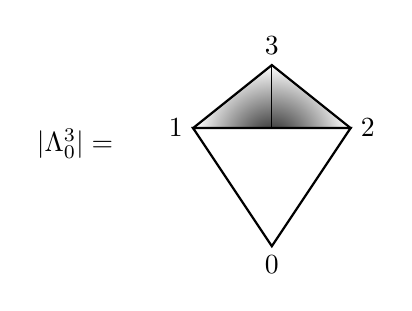
\begin{tikzpicture}
		\coordinate (A) at (0, 0);
		\coordinate (B) at (2, 0);
		\coordinate (C) at (1, 0.8);
		\coordinate (O) at (1, -1.5);
		
		\filldraw[thick, shading=radial, inner color=black!90, outer color=white] (A) node[left] {$1$} -- (C) node[above] {$3$} -- (B) node[right] {$2$} --($(O)!0.15!(C)$) --cycle;
		\draw (C) -- (O) node[below] {$0$};
		\filldraw[fill=white, thick] (A) -- (B) -- (O) --cycle;
		
		\node at ($(A) + (-1.5, -0.2)$) {$|\Lambda^3_0| =$};
	\end{tikzpicture}\end{center}
\end{example}

\begin{example}\label{eg:cone-realization}
	\index{danchunxingji!锥 (cone)}
	对任意拓扑空间 $\mathcal{X}$, 按自明的方式定义其上的锥 $\Cone_{\mathrm{top}}(\mathcal{X})$ 为将 $\mathcal{X} \times [0, 1]$ 的闭子集 $\mathcal{X} \times \{0\}$ 收缩为一个点的产物, 形象地看:
	\[\Cone_{\mathrm{top}}(\mathcal{X}) = \; 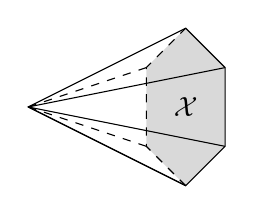
\begin{tikzpicture}[baseline=(P)]
		\coordinate (A) at (0, 1);
		\coordinate (B) at (0.5, 0.5);
		\coordinate (C) at (0.5, -0.5);
		\coordinate (D) at (0, -1);
		\coordinate (E) at (-0.5, -0.5);
		\coordinate (F) at (-0.5, 0.5);
		\coordinate (O) at (-2, 0);
		\coordinate (P) at (0, -0.1);	% For the baseline
		
		\fill[gray!50, opacity=0.6] (A) -- (B) -- (C) -- (D) -- (E) -- (F) --cycle;
		\draw (O) -- (A) -- (B) -- (C) -- (D) --cycle;
		\draw (O) -- (B);
		\draw (O) -- (C);
		\draw (O) -- (D);
		\draw[dashed] (D) -- (E) -- (F) -- (A);
		\draw[dashed] (O) -- (E);
		\draw[dashed] (O) -- (F);
		\node at (0, 0) {$\mathcal{X}$};
	\end{tikzpicture}\]
	作为一则简单练习, 请读者说明 $|X^{\lhd}| \simeq \Cone_{\mathrm{top}}(|X|) \simeq |X^{\rhd}|$. 这表明定义 \ref{def:cone-simplicial} 的锥名副其实, 左锥和右锥的差别仅在于定向.
\end{example}

通过将空间剖分为单纯形集, 可以萃取许多重要的拓扑性质, 这一进路被贴切地称为``组合拓扑学''. 进一步的讨论与实例可见 \cite[第六章]{You}.

\begin{definition}[奇异集函子]
	\index[sym1]{Sing@$\mathrm{Sing}$}
	\index{qiyiji@奇异集 (singular set)}
	对任意拓扑空间 $E$, 定义单纯形集 $\mathrm{Sing}(E)$ 使得
	\[ \mathrm{Sing}(E)_n := \Hom_{\cate{Top}}(|\Delta^n|, E), \quad n \in \Z_{\geq 0}, \]
	而 $d_i: \mathrm{Sing}(E)_n \to \mathrm{Sing}(E)_{n-1}$ (或 $s_j: \mathrm{Sing}(E)_n \to \mathrm{Sing}(E)_{n+1}$) 是沿着 $|\mathrm{d}^i|: |\Delta^{n-1}| \to |\Delta^n|$ (或 $|\mathrm{s}^j|: |\Delta^{n+1}| \to |\Delta^n|$) 的拉回, 称之为 $E$ 对应的奇异 (单纯形) 集. 这给出函子
	\[ \mathrm{Sing}: \cate{Top} \to \cate{sSet}. \]
\end{definition}

\begin{theorem}\label{prop:geom-Sing-adjunction}
	几何实现是奇异集的左伴随, 换言之, 有互逆映射
	\[\begin{tikzcd}[row sep=tiny]
		\Hom_{\cate{Top}}(|X|, E) \arrow[leftrightarrow, r, "1:1"] & \Hom_{\cate{sSet}}(X, \mathrm{Sing}(E)) \\
		\varphi \arrow[mapsto, r] & {\left[ X_n \xrightarrow{x \mapsto \varphi \circ i_{n, x}} \Hom_{\cate{Top}}(|\Delta^n|, E) \right]} \\
		\displaystyle\varinjlim_{(n, x)} \left( |\Delta^n| \xrightarrow{\psi_n(x)} E \right) & \psi = {\left[ \psi_n: X_n \to \Hom_{\cate{Top}}(|\Delta^n|, E) \right]}_{n \geq 0} , \arrow[mapsto, l]
	\end{tikzcd}\]
	其中 $X \in \Obj(\cate{sSet})$ 而 $E \in \Obj(\cate{Top})$.
\end{theorem}
\begin{proof}
	回忆到 $|X| = \varinjlim_{n, x} |\Delta^n|$. 我们有典范同构
	\begin{align*}
		\Hom_{\cate{Top}}\left( \varinjlim_{n, x} |\Delta^n| , E \right) & \rightiso \varprojlim_{n, x} \Hom_{\cate{Top}}(|\Delta^n|, E) = \varprojlim_{n, x} \mathrm{Sing}(E)_n \\
		& \rightiso \varprojlim_{n, x} \Hom_{\cate{sSet}}\left( \Delta^n, \mathrm{Sing}(E) \right) \\
		\varphi & \mapsto \left( \psi_n(x) := \varphi \circ i_{n, x} \right)_{n, x}. 
	\end{align*}
	
	任何 $\psi: X \to \mathrm{Sing}(E)$ 确定的态射族 $(\psi_n(x))_{n, x}$ 皆满足相容性, 亦即属于上式右侧的 $\varprojlim$. 若能说明指定态射 $\psi$ 相当于指定相容态射族, 证明便告完成, 然而这正是注记 \ref{rem:simplicial-density} 所确保的.
\end{proof}

\begin{remark}
	对于同伦论的研究, \S\ref{sec:closed-monoidal} 提及的 $\cate{CGHaus}$ 或许是比 $\cate{Top}$ 更方便的范畴. 由于包含函子 $\cate{CGHaus} \to \cate{Top}$ 有右伴随 $k$, 因而保 $\varinjlim$, 而 $|\Delta^n|$ 是紧生成 Hausdorff 空间, 故几何实现 (或奇异集) 中的黏合 (或取 $\Hom$) 可在 $\cate{CGHaus}$ 中操作\footnote{需要说明的是所论 $\varinjlim$ 在 $\cate{CGHaus}$ 中存在, 这步是拓扑的, 参见 \cite[III.1.8, III.2.1]{GZ67}.}. 定理 \ref{prop:geom-Sing-adjunction} 中的伴随对因之分成两段, 且以相同的符号记为
	\[\begin{tikzcd}
		\cate{sSet} \arrow[shift left, r, "{|\cdot|}"] & \cate{CGHaus} \arrow[shift left, r, "\text{包含函子}"] \arrow[shift left, l, "\mathrm{Sing}"] & \cate{Top} \arrow[shift left, l, "k"] .
	\end{tikzcd}\]
\end{remark}

对于任两个单纯形集 $X$ 和 $Y$, 它们的积定义为逐项积:
\begin{gather*}
	(X \times Y)_n = X_n \times Y_n, \\
	d_i(x, y) = (d_i(x), d_i(y)), \\
	s_j(x, y) = (s_j(x), s_j(y)).
\end{gather*}
这既是 $\cate{sSet} = \cate{Set}^{\simpDelta^{\opp}}$ 中的积, 又是在定义 \ref{def:monoidal-sObj} 中取幺半范畴 $(\cate{Set}, \times)$ 的产物. 尽管两者都是缘自范畴论的定义, 但以下的基本结果说明它们也承载几何意义.

\begin{theorem}\label{prop:realization-product}
	对于单纯形集 $X$ 和 $Y$, 我们有 $\cate{CGHaus}$ 中的典范同构
	\[ |X \times Y| \simeq |X| \times |Y|. \]
	推而广之, $\cate{CGHaus}$ 版本的 $|\cdot|$ 保有限 $\varprojlim$. 如果要求 $X$ 和 $Y$ 其中之一仅有有限多个非退化单纯形, 则 $|X \times Y| \simeq |X| \times |Y|$ 在 $\cate{Top}$ 中也成立. 
\end{theorem}

一般情形的证明颇费力, 可见 \cite[Chapter III]{GZ67} 或 \cite{Dri03}. 同构对几何实现的 $\cate{Top}$ 版本一般而言并不成立; 注意到定理对 $\cate{Top}$ 版本给出的条件并非最优.

\begin{corollary}
	记 $\cate{Grp}$ 为群范畴, 若单纯形集 $X$ 可以升级为 $\cate{sGrp}$ 的对象, 则 $|X|$ 也自然地具有拓扑群的结构; 对于其他代数结构也有类似的结果.
\end{corollary}

基于定理 \ref{prop:realization-product}, 我们有理由为 $\cate{sSet}$ 中的态射 $f, g: X \rightrightarrows Y$ 定义从 $g$ 到 $f$ 的同伦为态射 $H: X \times \Delta^1 \to X$, 使得下图交换:
\begin{equation}\label{eqn:simplicial-homotopy-prep}
	\begin{tikzcd}
		X \times \Delta^0 \arrow[d, "{\identity_X \times \mathrm{d}^0}"'] \arrow[r, "\sim"] & X \arrow[d, "f"] \\
		X \times \Delta^1 \arrow[r, "H" description] & Y \\
		X \times \Delta^0 \arrow[u, "{\identity_X \times \mathrm{d}^1}"] \arrow[r, "\sim"'] & X \arrow[u, "g"']
	\end{tikzcd}
\end{equation}

作为特例, $X \times \Delta^1 \xrightarrow{\text{投影}} X \xrightarrow{f} Y$ 的合成给出从 $f$ 到自身的常值同伦. 然而这般定义的同伦并非等价关系: 简单的例子足以说明它不满足对称性. 在同伦论中, 一般会要求 $Y$ 具有额外的性质, 比如是所谓的 Kan 复形. 此时同伦关系具有期望中的性质, 从而可以组合地开展同伦群, 弱等价等概念的研究.

尽管本书不证明定理 \ref{prop:realization-product}, 但针对 $X = \Delta^p$ 和 $Y = \Delta^q$ 的简单特例不妨多说几句. 比方说, 如何分类 $\Delta^p \times \Delta^q$ 的非退化单纯形? 问题的答案非但有助于理解积的几何实现, 相关构造也是之后需要的.

首先, 任两个偏序集 $S_1$ 和 $S_2$ 的积 $S_1 \times S_2$ 通过 $(a_1, a_2) \leq (b_1, b_2) \iff a_1 \leq b_1, \; a_2 \leq b_2$ 成为偏序集, 这也相当于将它们对应的范畴取积.

\begin{definition}\label{def:pq-shuffle}
	\index{pq-chongzu@$(p, q)$-重组 ($(p, q)$-shuffle)}
	设 $p, q \in \Z_{\geq 0}$. 所谓 \emph{$(p, q)$-重组}, 意谓一个保序单映射 $\sigma: [p+q] \to [p] \times [q]$.
\end{definition}

对任意 $n \in \Z_{\geq 0}$, 指定保序映射 $\sigma: [n] \to [p] \times [q]$ 相当于指定一对保序映射 $\sigma_-: [n] \to [p]$ 和 $\sigma_+: [n] \to [q]$; 这也相当于指定 $\Delta^p \times \Delta^q$ 的一个 $n$-单纯形. 要求 $\sigma$ 单相当于要求 $i \mapsto (\sigma_-(i), \sigma_+(i))$ 的轨迹不停顿 ($i = 0, \ldots, n$). 对于 $n = p+q$ 的情形, 状况图解为:
\begin{equation}\label{eqn:pq-shuffle-diag}
	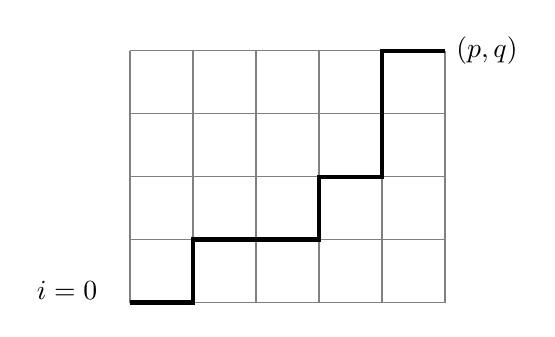
\begin{tikzpicture}[scale=0.8, baseline=(O)]
		\draw[thin, gray] (0, 0) grid (5, 4);
		\node at (-1, 0.2) {$i=0$};
		\draw[ultra thick] (0, 0) -- (1, 0) -- (1, 1) -- (2, 1) -- (3, 1) -- (3, 2) -- (4, 2) -- (4, 3) -- (4, 4) -- (5, 4) node[right] {$(p, q)$};
		\coordinate (O) at (0, 2);
	\end{tikzpicture}
	\quad
	\text{恰好移动 $p+q$ 步.}
\end{equation}
于是对于 $(p, q)$-重组 $\sigma$ 可以定义
\begin{align*}
	I_\pm & := \left\{ 1 \leq i \leq p+q : \sigma_\pm(i-1) < \sigma_\pm(i) \right\} \\
	& = \left\{ 1 \leq i \leq p+q : \sigma_\pm(i-1) = \sigma_\pm(i) - 1 \right\} \\
	& = \left\{ 1 \leq i \leq p+q: \sigma_\mp(i-1) = \sigma_\mp(i) \right\},
\end{align*}
它们满足 $I_+ \sqcup I_- = \{1, \ldots, p+q \}$. 子集 $I_+$ (或 $I_-$) 对应 \eqref{eqn:pq-shuffle-diag} 的上行 (或右行) 部分, 故 $(p, q)$-重组的另一种观点是视之为 $p$ 个符号 $\rightarrow$ 和 $q$ 个符号 $\uparrow$ 的排列, 共有 $\binom{p+q}{p}$ 种. 这些观察顺带说明 $\sigma_+$ 和 $\sigma_-$ 对于 $(p, q)$-重组是保序满射.

\begin{proposition}
	设 $p, q \in \Z_{\geq 0}$. 考虑 $\Delta^p \times \Delta^q$ 的 $n$-单纯形, 亦即保序映射 $\sigma: [n] \to [p] \times [q]$. 命 $(p_i, q_i) := \sigma(i)$, $(p', q') := (p_n - p_0, q_n - q_0)$, 则 $\sigma$ 非退化当且仅当下述条件成立:
	\begin{itemize}
		\item $p' + q' = n$;
		\item $\sigma$ 分解为 $(p', q')$-重组 $\sigma': [n] \to [p'] \times [q']$ 和形如 $f \times g$ 的保序单射 $[p'] \times [q'] \hookrightarrow [p] \times [q]$.
	\end{itemize} 
\end{proposition}
\begin{proof}
	让 $\sigma$ 对应到保序映射对 $(\sigma_-, \sigma_+)$. 按类似图 \eqref{eqn:pq-shuffle-diag} 的方式考虑 $i \mapsto (p_i, q_i)$ 的轨迹, $\sigma$ 非退化相当于说轨迹不停顿. 其余都是明白的.
\end{proof}

基于非退化单纯形的描述, 读者不妨发挥想象力来揣摩 $|\Delta^p \times \Delta^q| \simeq |\Delta^p| \times |\Delta^q|$ 在 $(p, q) = (1, 1)$ 和 $(2, 1)$ 时的道理. 例如下图是将 $|\Delta^2| \times |\Delta^1|$ 剖分为 $3$ 个四面体的结果, 对应于 $3 = \binom{3}{2}$ 个 $(2, 1)$-重组.

\begin{center}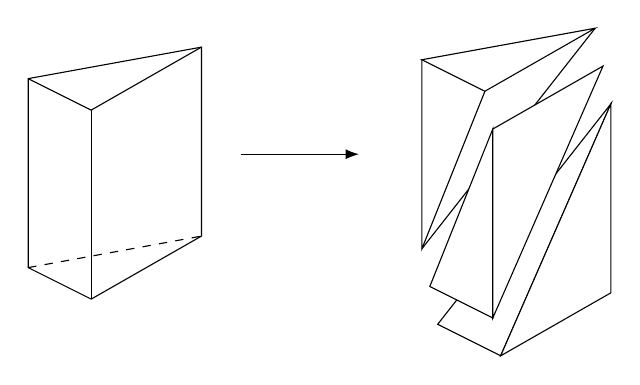
\begin{tikzpicture}[yscale=0.8]
	\coordinate (A) at (0, 0);
	\coordinate (B) at (2.2, 0.5);
	\coordinate (C) at (0.8, -0.5);
	\coordinate (P) at ($(A) + (0, -3)$);
	\coordinate (Q) at ($(B) + (0, -3)$);
	\coordinate (R) at ($(C) + (0, -3)$);

	\draw ($(A) + (-5, -0.3)$) -- ($(B) + (-5, -0.3)$) -- ($(Q) + (-5, -0.3)$) -- ($(R) + (-5, -0.3)$) -- ($(P) + (-5, -0.3)$) --cycle;
	\draw ($(A) + (-5, -0.3)$) -- ($(C) + (-5, -0.3)$) -- ($(B) + (-5, -0.3)$);
	\draw ($(C) + (-5, -0.3)$) -- ($(R) + (-5, -0.3)$);
	\draw[dashed] ($(P) + (-5, -0.3)$) -- ($(Q) + (-5, -0.3)$);
	
	\draw[-Latex] ($(B)!0.5!(Q) + (-4.5, -0.5)$) -- ($(B)!0.5!(Q) + (-3, -0.5)$);
	
	\draw (A) -- (B) -- (C) --cycle;
	\draw (A) -- (P) -- (C);
	\draw (P) -- (B);
	
	\draw[fill=white] ($(P) + (0.2, -1.2)$) -- ($(B) + (0.2, -1.2)$) -- ($(R) + (0.2, -1.2)$) --cycle;
	\draw[fill=white] ($(R) + (0.2, -1.2)$) -- ($(Q) + (0.2, -1.2)$) -- ($(B) + (0.2, -1.2)$) --cycle;
	
	\draw[fill=white] ($(P) + (0.1, -0.6)$) -- ($(R) + (0.1, -0.6)$) -- ($(C) + (0.1, -0.6)$) --cycle;
	\draw[fill=white] ($(R) + (0.1, -0.6)$) -- ($(B) + (0.1, -0.6)$) -- ($(C) + (0.1, -0.6)$) --cycle;
\end{tikzpicture}\end{center}

\begin{definition}\label{def:pq-shuffle-sgn}
	设 $\sigma$ 为 $(p, q)$-重组, 其符号定义为
	\[ \sgn(\sigma) := (-1)^{|I_\sigma|}, \quad I_\sigma := \left\{ (i, j) \in I_- \times I_+ : i > j \right\}. \]
\end{definition}

若将 $\sigma$ 视同 $p$ 个 $\rightarrow$ 和 $q$ 个 $\uparrow$ 的排列, 则 $I_\sigma$ 便是所有出现``错排'' $(\uparrow, \rightarrow)$ 的数对 $(j, i)$, 其中 $j < i$. 简单的组合学练习足以说明存在唯一的 $\tau \in \mathfrak{S}_{p+q}$ 将这般排列还原为形如 $\rightarrow \cdots \rightarrow \uparrow \cdots \uparrow$ 的样式, 而不打乱 $I_+$ 和 $I_-$ 内部的顺序, 而定义 \ref{def:pq-shuffle-sgn} 相当于说 $\sgn(\sigma) = \sgn(\tau)$.

对于 $(p, q)$-重组 $\sigma$, 调换 $\sigma_-$ 和 $\sigma_+$ 的角色给出 $(q, p)$-重组 $\sigma'$. 上述诠释和基本的组合学论证表明
\begin{equation}\label{eqn:shuffle-sign-0}
	\sgn(\sigma) = (-1)^{pq} \sgn(\sigma').
\end{equation}

准此要领, 类似地定义 $(p, q, r)$-重组为保序单射 $\sigma = (\sigma_-, \sigma_0, \sigma_+): [p+q+r] \to [p] \times [q] \times [r]$, 或理解为符号 $\rightarrow$, $\nearrow$, $\uparrow$ 的排列, 并且定义 $\sgn(\sigma)$ 为 $(-1)^{|I_\sigma|}$, 其中 $I_\sigma$ 由所有对应于 $(\rightarrow, \nearrow, \uparrow)$ 的奇排列的数组 $k > j > i$ 构成. 同样标准的组合学练习表明若 $(p, q, r)$-重组 $\sigma$ 有分解
\[ [p+q+r] \xrightarrow{\sigma_1} [p+q] \times [r] \xrightarrow{\sigma_2 \times \identity_{[r]}} [p] \times [q] \times [r], \]
则 $\sigma_1$ 是 $(p+q, r)$-重组, $\sigma_2$ 是 $(p, q)$-重组, 而且
\begin{equation}\label{eqn:shuffle-sign-1}
	\sgn(\sigma) = \sgn(\sigma_1) \sgn(\sigma_2).
\end{equation}
对于分解 $[p+q+r] \to [p] \times [q+r] \to [p] \times [q] \times [r]$ 自然也有对应的陈述.

等式 \eqref{eqn:shuffle-sign-0} 和 \eqref{eqn:shuffle-sign-1} 的本质都是组合学, 详细验证留作本章习题. 这些观察将在 \S\ref{sec:bisimplicial} 用到.

\section{Dold--Kan 对应}\label{sec:Dold-Kan}
遵循代数拓扑学的惯例, 我们将对加性范畴 $\mathcal{A}$ 考虑其上的链复形范畴 (定义 \ref{def:complex}), 记为 $\cate{Ch}(\mathcal{A})$, 连同其子范畴
\[ \cate{Ch}_{\geq 0}(\mathcal{A}) := \left\{ A = (A_n, \partial_n)_{n \in \Z} : \text{链复形}, \; \forall n < 0, \; A_n = 0 \right\}, \]
其中 $\partial_n = \partial^A_n: A_n \to A_{n-1}$. 对于 $\cate{Ch}_{\geq 0}(\mathcal{A})$ 显然只需指定资料 $(A_n)_{n \geq 0}$ 和 $(\partial_n)_{n \geq 1}$. 同理可以定义 $\cate{Ch}_{\geq m}(\mathcal{A})$; 请参照定义 \ref{def:cplx-cat-variant} 的上链复形版本.
\index[sym1]{ChA@$\cate{Ch}(\mathcal{A})$}

适当扩大所取的 Grothendieck 宇宙, 不妨假定 $\mathcal{A}$ 是加性小范畴, 见 \cite[假设 1.5.2]{Li1}. 从 $\mathcal{A}$ 可以定义单纯形对象范畴 $\cate{s}\mathcal{A}$; 对应于 $0$ 的常值单纯形对象仍记为 $0 \in \Obj(\cate{s}\mathcal{A})$. 本节旨在初步地明确这些范畴之间的关系, 更精确地说, 我们将定义三个函子
\[\begin{tikzcd}
	\cate{Ch}_{\geq 0}(\mathcal{A}) \arrow[r, "\Gamma" description] & \cate{s}\mathcal{A} \arrow[bend left, l, "{\mathrm{N}}"] \arrow[bend right, l, "{\mathrm{C}}"']
\end{tikzcd}\]
其中 $\mathrm{N}$ 仅在 $\mathcal{A}$ 为 Abel 范畴时方有定义, 而 $\mathrm{C}$ 和 $\mathrm{N}$ 都可以扩及注记 \ref{rem:semisimplicial} 所谓的半单纯形对象; 换言之, 它们不涉及退化态射.

我们的处理方式取法 \cite[\S 1.2]{LuHA}. 首务是明确相关定义.

\begin{definition}[非正规化链复形]\label{def:unnormalized-chain}
	\index{feizhengguihualianfuxing@非正规化链复形 (unnormalized chain complex)}
	\index{Moore lianfuxing@Moore 链复形 (Moore chain complex)}
	\index[sym1]{CX@$\mathrm{C}X$}
	对于 $\mathcal{A}$ 中的半单纯形对象 $X$ 和每个 $n \in \Z_{\geq 1}$, 定义
	\[ \partial_n := \sum_{i=0}^n (-1)^i d_i: X_n \to X_{n-1}; \]
	这使得 $(X_n)_{n \geq 0}$ 连同 $(\partial_n)_n$ 构成 $\cate{Ch}_{\geq 0}(\mathcal{A})$ 的对象, 称为 $X$ 给出的\emph{非正规化链复形}或 \emph{Moore 链复形}, 记为 $\mathrm{C}X$; 因此 $(\mathrm{C}X)_n = X_n$.
\end{definition}

必须说明当 $n > 1$ 时 $\partial_{n-1}\partial_n = 0$; 诚然, \eqref{eqn:simplicial-identity} 中的 $i < j \implies d_i d_j = d_{j-1} d_i$ 蕴涵
\begin{multline*}
	\partial_{n-1} \partial_n = \sum_{i=0}^{n-1} \sum_{j=0}^n (-1)^{i+j} d_i d_j \\
	= \sum_{0 \leq i < j \leq n} (-1)^{i+j} d_{j-1} d_i + \sum_{n-1 \geq i \geq j \geq 0} (-1)^{i+j} d_i d_j = 0.
\end{multline*}
此构造对 $X$ 显然是典范的, 给出函子 $\mathrm{C}$.

\begin{example}\label{eg:classifying-space-std-cplx}
	取交换环 $\Bbbk$ 和 $\mathcal{A} = \Bbbk\dcate{Mod}$. 给定群 $\Gamma$, 例 \ref{eg:classifying-space} 给出对应的单纯形集 $\mathrm{E}\Gamma$; 定义 $\Bbbk\dcate{Mod}$ 上的单纯形对象 $\Bbbk\mathrm{E}\Gamma$, 它的 $n$ 次项是以 $\mathrm{E}\Gamma$ 为基的自由 $\Bbbk$-模, $d_i$ 和 $s_i$ 则按线性延拓. 兹断言 $\mathrm{C}(\Bbbk \mathrm{E}\Gamma)$ 正是定义 \ref{def:resolution-trivial-module} 介绍的链复形 $\mathsf{L} := (\mathsf{L}_n, \partial'_n)_n$. 首先, $\mathsf{L}_n$ 按定义是以 $\Gamma^{n+1}$ 为基的自由 $\Bbbk$-模. 取从 $(\mathrm{E}\Gamma)_n = \Gamma^{n+1}$ 到 $\mathsf{L}_n$ 的映射
	\[ \left( g_1, \ldots, g_{n+1} \right) \mapsto \left(g_1 \cdots g_{n+1}, \; \ldots , \; g_n g_{n+1}, \; g_{n+1}\right). \]
	它线性地延拓到 $(\Bbbk\mathrm{E}\Gamma)_n$ 上. 请读者验证 $\sum_i (-1)^i d_i$ 依此对应到 $\partial'_n: \mathsf{L}_n \to \mathsf{L}_{n-1}$, 给出所求同构.
	
	此外, $\Gamma$ 通过 $(g_1, \ldots, g_{n+1}) \xmapsto{g} (g_1, \ldots, g_n, g_{n+1}g)$ 右作用于每个 $(\mathrm{E}\Gamma)_n$; 这反映在 $\mathsf{L}_n$ 的基上, 化作 $(g_0, \ldots, g_n) \xmapsto{g} (g_0 g, \ldots, g_n g)$; 于是我们得到定义 \ref{def:resolution-trivial-module} 赋予 $\mathsf{L}$ 的右 $\Gamma$-作用. 有鉴于此, 对链复形 $\mathrm{C}(\Bbbk\mathrm{E}\Gamma)$ 和 $\mathsf{L}$ 逐项取 $\Gamma$-余不变量的产物也相互同构, 而前者又相当于对 $\mathrm{E}\Gamma$ 逐项取商再取自由 $\Bbbk$-模. 这导致
	\[ \mathrm{C}(\Bbbk\mathrm{B}\Gamma) \simeq \mathsf{L} \dotimes{\Bbbk[\Gamma]} \Bbbk, \]
	张量积涉及增广同态 $\Bbbk[\Gamma] \to \Bbbk$; 作为推论, 群的同调 (定义 \ref{def:group-coh-ho}) 便诠释为
	\[ \Hm_n(\mathrm{B}\Gamma; \Bbbk) := \Hm_n \mathrm{C}(\Bbbk\mathrm{B}\Gamma) \simeq \Hm_n(\Gamma, \Bbbk), \quad n \in \Z_{\geq 0}. \]
	
	左式出现了单纯形集的同调, 这是定义 \ref{def:simplicial-set-homology} 即将介绍的一般构造. 本章习题将对 $\mathsf{L}$ 的正规化版本 $\overline{\mathsf{L}}$ 给出类似的同构, 它对应于定义 \ref{def:normalized-cplx} 行将讨论的正规化链复形 $\mathrm{N}(\Bbbk\mathrm{E}\Gamma)$.
\end{example}

\begin{definition}\label{def:DK-Gamma}
	取定 $\cate{Ch}_{\geq 0}(\mathcal{A})$ 的对象 $(A_n, \partial_n)_{n \geq 0}$. 按以下方式定义 $\cate{s}\mathcal{A}$ 的对象 $\Gamma(A)$.
	\[ (\Gamma A)_n := \bigoplus_{t: [n] \twoheadrightarrow [k]} A_k. \]
	
	对于 $\simpDelta$ 的任意态射 $f: [m] \to [n]$, 对应的 $f^*: (\Gamma A)_n \to (\Gamma A)_m$ 相对于上述直和分解表为以下矩阵 
	\[ \left( \Phi_{u, t} : A_k \to A_l \right)_{\substack{ u: [m] \twoheadrightarrow [l] \\ t: [n] \twoheadrightarrow [k] }}, \]
	按以下方式确定: 给定 $t: [n] \twoheadrightarrow [k]$, 作 $tf$ 的满--单分解
	\begin{equation}\label{eqn:Dold-Kan-epi-mono}\begin{tikzcd}[row sep=tiny]
		& {[n]} \arrow[twoheadrightarrow, rd, "t"] & \\
		{[m]} \arrow[ru, "f"] \arrow[twoheadrightarrow, rd, "u"'] & & {[k]} \\
		& {[l]} \arrow[hookrightarrow, ru, "v"'] &
	\end{tikzcd}\end{equation}
	\begin{itemize}
		\item 若 $l = k$, 命 $\Phi_{u, t} = \identity$;
		\item 若 $l = k-1$ 而 $v = \mathrm{d}^0$ (遗漏 $0$ 的保序单射), 命 $\Phi_{u, t} = \partial_k: A_k \to A_{k-1}$;
		\item 其余情形命 $\Phi_{u, t} = 0$.
	\end{itemize}
	留意到当 $f$ 和 $t$ 给定, 至多仅有唯一的 $u$ 使 $\Phi_{u, t} \neq 0$.
\end{definition}

关于 $\Gamma A \in \Obj(\cate{s}\mathcal{A})$ 的验证比较琐碎, 在此略过. 核心是 $(\Gamma A)_n$ 的直和项 $A_n$ 和它们在保序单映射下的行为, 其他低次直和项 $A_k$ 皆来自满态射 $[n] \twoheadrightarrow [k]$ 诱导的退化, 一般情形下 $f^*$ 的定义不过是体现此思路.

上述构造是典范的, 给出函子 $\Gamma: \cate{Ch}_{\geq 0}(\mathcal{A}) \to \cate{s}\mathcal{A}$.

\begin{definition}\label{def:normalized-cplx}
	\index{zhengguihualianfuxing@正规化链复形 (normalized chain complex)}
	\index[sym1]{NX@$\mathrm{N}X$}
	设 $\mathcal{A}$ 是 Abel 范畴. 对 $\mathcal{A}$ 中的半单纯形对象 $X$ 和所有 $n \in \Z_{\geq 0}$ 和 $0 \leq k \leq n$ 定义
	\begin{align*}
		(\mathrm{N} X)_n & := \bigcap_{i=1}^n \Ker\left[ d_i: X_n \to X_{n-1} \right], \quad n \geq 1, \\
		(\mathrm{N} X)_0 & := X_0.
	\end{align*}

	连同 $X_n \xrightarrow{d_0} X_{n-1}$ 所诱导的态射族 $\mathrm{N}X_n \to \mathrm{N}X_{n-1}$ (请用 \eqref{eqn:simplicial-identity} 验证), 合理地记为 $\partial_n$, 它们构成 $\cate{Ch}_{\geq 0}(\mathcal{A})$ 的对象 $\mathrm{N}X$, 称为 $X$ 对应的\emph{正规化链复形}.
\end{definition}

\begin{proposition}\label{prop:Dold-Kan-u}
	对如上之 $X$ 和每个 $n \geq 0$, 记 $u_n: (\mathrm{N}X)_n \hookrightarrow X_n$ 为自然嵌入, 则 $(u_n)_{n \geq 0}$ 构成 $\cate{Ch}_{\geq 0}(\mathcal{A})$ 中的单态射 $u: \mathrm{N}X \to \mathrm{C}X$, 它对 $X$ 满足函子性.
\end{proposition}
\begin{proof}
	直接来自 $\mathrm{N}X$ 和 $\mathrm{C}X$ 的定义.
\end{proof}

后续几则结果是 Dold--Kan 定理 \ref{prop:Dold-Kan} 的必要铺垫.

\begin{lemma}\label{prop:DK-N-unit}
	设 $\mathcal{A}$ 是 Abel 范畴, 则对所有 $A \in \Obj(\cate{Ch}_{\geq 0}(\mathcal{A}))$ 和 $n \geq 0$ 皆有 $\mathrm{N}\Gamma(A)_n = A_n$. 这给出函子的同构 $\eta: \identity_{\cate{Ch}_{\geq 0}(\mathcal{A})} \rightiso \mathrm{N}\Gamma$.
\end{lemma}
\begin{proof}
	给定 $t: [n] \twoheadrightarrow [k]$, 注意到当 $k < n$ 时, 总可以取 $1 \leq i \leq n$ 使得 $t^{-1}(t(i))$ 至少有两个元素, 从而 $t \mathrm{d}^i$ 满, 使下图交换:
	\[\begin{tikzcd}[row sep=tiny]
		& {[n]} \arrow[twoheadrightarrow, rd, "t"] & \\
		{[n-1]} \arrow[ru, "{\mathrm{d}^i}"] \arrow[twoheadrightarrow, rd, "{t\mathrm{d}^i}"'] & & {[k]} \\
		& {[k]} \arrow[ru, "{\identity}"'] &
	\end{tikzcd}\]
	代入定义 \ref{def:DK-Gamma} 遂知 $\mathrm{N}\Gamma(A)_n$ 包含于 $\identity: [n] \to [n]$ 对应的直和项 $A_n$. 然而易证该定义进一步蕴涵 $\mathrm{N}\Gamma(A)_n = A_n$, 而且 $\mathrm{N}\Gamma(A)_{n+1} \to \mathrm{N}\Gamma(A)_n$ 正是 $\partial_{n+1}: A_{n+1} \to A_n$. 证毕.
\end{proof}

\begin{lemma}\label{prop:GammaN-adjunction}
	设 $\mathcal{A}$ 是 Abel 范畴, 则先前定义的函子给出伴随对
	\[\begin{tikzcd}
		\Gamma: \cate{Ch}_{\geq 0}(\mathcal{A}) \arrow[shift left, r] & \cate{s}\mathcal{A} : \mathrm{N} \arrow[shift left, l]
	\end{tikzcd}\]
	\begin{itemize}
		\item 对应的单位态射是引理 \ref{prop:DK-N-unit} 的同构 $\eta$;
		\item 余单位态射 $\epsilon: \Gamma \mathrm{N}\to \identity_{\cate{s}\mathcal{A}}$ 描述如下: 给定 $t: [n] \twoheadrightarrow [k]$, 在 $\Gamma\mathrm{N}(X)_n$ 中相应的直和项 $(\mathrm{N}X)_k$ 上, $\epsilon_{X, n}$ 是 $(\mathrm{N}X)_k \subset X_k \xrightarrow{t^*} X_n$.
	\end{itemize}
\end{lemma}
\begin{proof}
	给定 $A \in \Obj(\cate{Ch}_{\geq 0}(\mathcal{A}))$ 和 $X \in \Obj(\cate{s}\mathcal{A})$, 首要目标是证
	\[ \Hom_{\cate{s}\mathcal{A}}(\Gamma(A), X) \xrightarrow{\mathrm{N}} \Hom_{\cate{Ch}_{\geq 0}(\mathcal{A})}(\mathrm{N}\Gamma(A), \mathrm{N}(X)) \xrightarrow{\eta_A^*} \Hom_{\cate{Ch}_{\geq 0}(\mathcal{A})}(A, \mathrm{N}(X)) \]
	的合成为双射. 其逆具体定义如下. 给定 $\phi = (\phi_n)_{n \geq 0}: A \to \mathrm{N}(X)$, 定义态射
	\[ \Phi_n: (\Gamma A)_n = \bigoplus_{t: [n] \twoheadrightarrow [k]} A_k \to X_n \]
	使得它在对应 $t: [n] \twoheadrightarrow [k]$ 的直和项上是
	\[ A_k \xrightarrow{\phi_k} (\mathrm{N}X)_k \subset X_k \xrightarrow{t^*} X_n \]
	的合成. 对于如上之 $t$ 和任意的 $f: [m] \to [n]$, 作 $tf$ 的满--单分解如 \eqref{eqn:Dold-Kan-epi-mono}, 并考虑 $\mathcal{A}$ 中的图表 (参见定义 \ref{def:DK-Gamma}):
	\[\begin{tikzcd}[column sep=large]
		A_k \arrow[r, "\phi_k"] \arrow[d, "{\Phi_{u, t}}"'] & (\mathrm{N}X)_k \arrow[hookrightarrow, r] \arrow[d, "{v^*|_{(\mathrm{N}X)_k}}"] & X_k \arrow[r, "{t^*}"] \arrow[d, "{v^*}"] & X_n \arrow[d, "{f^*}"] \\
		A_l \arrow[r, "\phi_l"'] & (\mathrm{N}X)_l \arrow[hookrightarrow, r] & X_l \arrow[r, "{u^*}"'] & X_m
	\end{tikzcd}\]
	左侧方块因正规化链复形 $\mathrm{N}X$ 的定义而交换, 中间方块显然交换, 右侧方块因 $tf = vu$ 交换. 因此 $\Phi = (\Phi_n)_n$ 是 $\cate{s}\mathcal{A}$ 的态射.
	
	关于 $\eta_A^* \mathrm{N}$ 和 $\phi \mapsto \Phi$ 互逆的验证不过是例行公事. 在 $\phi \mapsto \Phi$ 的描述中取 $\phi = \identity_{\mathrm{N}X}$, 结果正是断言中的 $\epsilon$.
\end{proof}

\begin{lemma}\label{prop:DK-Ab}
	取 $\mathcal{A} = \cate{Ab}$, 则 $\Gamma$ 是等价; 精确地说, 伴随对
	$\begin{tikzcd}
		\Gamma: \cate{Ch}_{\geq 0}(\cate{Ab}) \arrow[shift left, r] & \cate{s}\cate{Ab} : \mathrm{N} \arrow[shift left, l]
	\end{tikzcd}$
	是 \cite[定理 2.6.12]{Li1} 所谓的伴随等价.
\end{lemma}
\begin{proof}
	要点在于验证引理 \ref{prop:GammaN-adjunction} 描述的余单位态射 $\epsilon$ 为同构. 选定 $X \in \Obj(\cate{s}\mathcal{A})$, 兹断言 $\epsilon_{X, n}: \Gamma (\mathrm{N}X)_n \to X_n$ 对每个 $n \geq 0$ 皆单. 设 $x = (x_t)_t$ 属于左式, 其中 $t$ 遍历保序满射 $[n] \twoheadrightarrow [k]$. 给定 $t$, 定义保序单射
	\begin{align*}
		s = s_t : [k] & \hookrightarrow [n] \\
		i & \mapsto \min t^{-1}(i) ,
	\end{align*}
	它满足 $ts = \identity_{[k]}$. 现在假定 $x \neq 0$, 记
	\[ S := \left\{t: x_t \neq 0 \right\} \neq \emptyset. \]
	取最小的 $k$ 使得存在属于 $S$ 的 $t: [m] \twoheadrightarrow [k]$, 再取如此之 $t$ 使 $\sum_{i=0}^k \min t^{-1}(i)$ 尽量小, 并构造 $s$. 今将往证 $s^*(\epsilon_{X, n}(x)) = x_t \in X_k$, 以此说明 $\epsilon_{X, n}(x) \neq 0$.
	
	基于 $\epsilon_{X, n}$ 的具体描述, 仅须对 $t': [n] \twoheadrightarrow [k']$ 证明 $s^* (t')^*(x_{t'}) \neq 0$ 蕴涵 $t = t'$ 即可. 命 $u := t's: [k] \to [k']$. 当 $t' \notin S$ 时 $x_{t'} = 0$, 故以下设 $t' \in S$ 满足 $s^* (t')^*(x_{t'}) = u^* (x_{t'}) \neq 0$.
	
	由于 $t$ 保序而且满, $\min t^{-1}(0) = 0$, 对 $t'$ 亦然, 故 $u(0) = 0$. 又由 $x_{t'} \in (\mathrm{N}X)_{k'}$ 可推知仅当 $\Image(u) \supset \{1, \ldots, k'\}$ 时才可能有 $u^* (x_{t'}) \neq 0$. 故以下可设 $u$ 满, $k$ 的取法遂蕴涵 $k' = k$ 而 $u = \identity$.
	
	综之, $t'\left( \min t^{-1}(i) \right) = i$ 对 $i = 0, \ldots, k$ 皆成立, 故 $\min (t')^{-1}(i) \leq \min t^{-1}(i)$. 回顾 $t$ 的取法可得 $\min (t')^{-1}(i) = \min t^{-1}(i)$ 对所有 $0 \leq i \leq k$ 成立; 稍加思索, 可知这相当于说 $t = t'$. 至此证得 $\epsilon_{X, n}$ 单.
	
	以下对 $n$ 递归地证明 $\epsilon_{X, n}$ 满. 兹断言对所有 $0 \leq i \leq n$ 皆有
	\[ \Image\left( \epsilon_{X, n} \right) \supset X(i)_n := \bigcap_{i < j \leq n} \Ker(d_j) \subset X_n. \]
	
	当 $i = 0$ 时 $X(i)_n = (\mathrm{N}X)_n$, 上式容易从 $\epsilon_{X, n}$ 的具体描述导出, 而我们的目标是 $i=n$. 设 $n \geq i \geq 1$ 而 $y \in X(i)_n$. 关于 $n-1$ 的递归假设和 $\epsilon_{X, n}$ 的描述蕴涵
	\[ s_{i-1} d_i(y) \in s_{i-1}\left( \Image\left(\epsilon_{X, n-1}\right) \right) \subset \Image\left( \epsilon_{X, n} \right). \]

	另一方面, 单纯形等式 \eqref{eqn:simplicial-identity} 蕴涵
	\begin{gather*}
		d_i s_{i-1} d_i = d_i, \\
		j > i \implies d_j s_{i-1} d_i = s_{i-1} d_{j-1} d_i = s_{i-1}  d_i d_j.
	\end{gather*}
	故 $y - s_{i-1} d_i(y) \in X(i-1)_n$, 而关于 $i-1$ 的递归假设说明它属于 $\Image\left( \epsilon_{X, n} \right)$. 综之 $y \in \Image\left( \epsilon_{X, n} \right)$, 明所欲证.
\end{proof}

\begin{theorem}[A.\ Dold, D.\ Kan]\label{prop:Dold-Kan}
	\index{Dold-Kan duiying@Dold--Kan 对应 (Dold--Kan correspondence)}
	对于任意加性范畴 $\mathcal{A}$, 函子 $\Gamma: \cate{Ch}_{\geq 0}(\mathcal{A}) \to \cate{s}\mathcal{A}$ 是全忠实的.
	\begin{itemize}
		\item 若 $\mathcal{A}$ 还是 \S\ref{sec:direct-sum} 提及的 Karoubi 范畴, 亦即所有幂等元都有核, 则 $\Gamma$ 是范畴等价.
		\item 若进一步要求 $\mathcal{A}$ 是 Abel 范畴 (因而也是 Karoubi 范畴), 则 $\mathrm{N}$ 是 $\Gamma$ 的拟逆函子,
		$\begin{tikzcd}
			\Gamma: \cate{Ch}_{\geq 0}(\mathcal{A}) \arrow[shift left, r] & \cate{s}\mathcal{A} : \mathrm{N} \arrow[shift left, l]
		\end{tikzcd}$
		是伴随等价, 伴随对的单位和余单位态射由引理 \ref{prop:GammaN-adjunction} 描述.
	\end{itemize}
\end{theorem}
\begin{proof}
	考虑函子
	\[ \tilde{h}_{\mathcal{A}}: \mathcal{A} \to \tilde{\mathcal{A}}^\wedge := \cate{Ab}^{(\mathcal{A}^{\opp})}, \quad Y \mapsto \Hom_{\mathcal{A}}(\cdot, Y). \]
	它和忘却函子 $\cate{Ab} \to \cate{Set}$ 合成等于 \S\ref{sec:Yoneda} 回顾的米田嵌入 $h_{\mathcal{A}}: \mathcal{A} \to \mathcal{A}^\wedge$. 函子 $\tilde{h}_{\mathcal{A}}$ 是全忠实的, 这点不过是 $\cate{Ab}$-充实版本的米田引理, 但也可以从原版推导: 对任意 $Y_1, Y_2 \in \Obj(\mathcal{A})$, 合成映射
	\[ \Hom_{\mathcal{A}}(Y_1, Y_2) \to \Hom_{\tilde{\mathcal{A}}^\wedge}\left(\tilde{h}_{\mathcal{A}}(Y_1), \tilde{h}_{\mathcal{A}}(Y_2) \right) \to \Hom_{\mathcal{A}^\wedge}\left( h_{\mathcal{A}}(Y_1), h_{\mathcal{A}}(Y_2)\right) \]
	已知是双射, 但第二段明显是单射, 由此可知两段皆为双射.
	
	命题 \ref{prop:functor-cat-Abel} 表明 $\tilde{\mathcal{A}}^\wedge$ 自然地成为 Abel 范畴. 以相同的符号标记 $\tilde{h}_{\mathcal{A}}$ 在链复形和单纯形对象上诱导的函子, 考虑图表:
	\begin{equation*}\begin{tikzcd}
		\cate{Ch}_{\geq 0}(\mathcal{A}) \arrow[d, "{\tilde{h}_{\mathcal{A}}}"'] \arrow[r, "\Gamma"] & \cate{s}\mathcal{A} \arrow[d, "{\tilde{h}_{\mathcal{A}}}"] \\
		\cate{Ch}_{\geq 0}(\tilde{\mathcal{A}}^\wedge) \arrow[r, "\Gamma"'] & \cate{s}\tilde{\mathcal{A}}^\wedge
	\end{tikzcd}\end{equation*}
	此图精确到典范同构是交换的. 上一段的观察说明两个垂直箭头全忠实, 而逐对象地应用关于 $\cate{Ab}$ 的引理 \ref{prop:DK-Ab}, 可见第二行是范畴等价. 于是第一行的 $\Gamma$ 全忠实.
	
	对于任意函子 $F: \mathcal{C} \to \mathcal{C}'$, 我们称 $X' \in \Obj(\mathcal{C}')$ 属于 $F$ 的本质像, 如果存在 $X \in \cate{Obj}(\mathcal{C})$ 使得 $X' \simeq FX$. 搭配引理 \ref{prop:DK-Ab} 对 $\cate{Ch}_{\geq 0}(\cate{Ab}) \to \cate{s}\cate{Ab}$ 的拟逆的描述, 便能得到以下结论: $X \in \Obj(\cate{s}\mathcal{A})$ 属于 $\Gamma$ 的本质像当且仅当 $\mathrm{N} \tilde{h}_{\mathcal{A}}(X)_n$ 对每个 $n \geq 0$ 皆属于 $\tilde{h}_{\mathcal{A}}: \mathcal{A} \to \tilde{\mathcal{A}}^\wedge$ 的本质像.
	
	注意到 $\tilde{h}_{\mathcal{A}}: \mathcal{A} \to \tilde{\mathcal{A}}^\wedge$ 保有限直和.
	当 $\mathcal{A}$ 是 Karoubi 范畴时, $\mathcal{A} \to \tilde{\mathcal{A}}^\wedge$ 的本质像因而对萃取直和项保持封闭; 既然 $\mathrm{N} \tilde{h}_{\mathcal{A}}(X)_n$ 是 $\Gamma\mathrm{N} \tilde{h}_{\mathcal{A}}(X)_n \simeq h_{\mathcal{A}}(X)_n$ 的直和项, 此时 $\Gamma$ 全忠实本质满, 从而是等价.
	
	最后, 伴随等价定理 \cite[定理 2.6.12]{Li1} 确保 $\Gamma: \cate{Ch}_{\geq 0}(\mathcal{A}) \to \cate{s}\mathcal{A}$ 的拟逆总能扩充为其右伴随. 当 $\mathcal{A}$ 是 Abel 范畴时, 引理 \ref{prop:GammaN-adjunction} 已经说明 $\mathrm{N}$ 是 $\Gamma$ 的右伴随, 因而是 $\Gamma$ 的拟逆. 明所欲证.
\end{proof}

\begin{convention}
	基于此, 当 $\mathcal{A}$ 是 Karoubi 范畴时, 可以选定 $\Gamma: \cate{Ch}_{\geq 0}(\mathcal{A}) \to \cate{s}\mathcal{A}$ 的拟逆函子, 并且合理地记之为 $\mathrm{N}$.
\end{convention}

虽然 $\mathrm{N}X$ 的初始定义是 $\mathrm{C}X$ 的子对象, 但是它也可以理解为商, 后者在很多场合更加方便. 以下便来说明这一点.

考虑 Karoubi 范畴 $\mathcal{A}$ 和 $X \in \Obj(\cate{s}\mathcal{A})$. 对所有 $n \geq 0$ 定义 $\mathcal{A}$ 中的态射 $\Psi_n$, 其刻画是使下图对所有 $0 \leq j < n$ 交换:
\[\begin{tikzcd}
	\bigoplus_{0 \leq i < n} X_{n-1} \arrow[r, "\Psi_n"] & X_n \\
	X_j \arrow[hookrightarrow, u, "\text{直和项}"] \arrow[ru, "{s_j}"'] &
\end{tikzcd}\]
因此考虑 $\Coker(\Psi_n)$ (亦即 $\Psi_n$ 和 $0$ 的余等化子) 相当于从 $X_n$ 抹去所有退化部分, 至少当 $\mathcal{A}$ 是 Abel 范畴时可作此观; 次一结果说明 $\Coker(\Psi_n)$ 不只存在, 还通过命题 \ref{prop:Dold-Kan-u} 的自然嵌入 $u: \mathrm{N}X \to \mathrm{C}X$ 等同于 $(\mathrm{N}X)_n$, 这就提供了看待 $\mathrm{N}X$ 的另一视角.

\begin{proposition}\label{prop:Dold-Kan-v}
	在上述情境中, $\Coker(\Psi_n)$ 存在并且典范同构于 $(\mathrm{N}X)_n$. 考虑相应的合成 $v_n: X_n \twoheadrightarrow \Coker(\Psi_n) \rightiso (\mathrm{N}X)_n$, 则 $(v_n)_n$ 给出态射 $v: \mathrm{C}X \to \mathrm{N}X$, 它对 $X$ 有函子性, 并且对自然嵌入 $u: \mathrm{N}X \hookrightarrow \mathrm{C}X$ 满足 $vu = \identity_{\mathrm{N}X}$.
\end{proposition}
\begin{proof}
	鉴于定理 \ref{prop:Dold-Kan}, 不妨假设 $X = \Gamma A$, 其中 $A \in \Obj(\cate{Ch}_{\geq 0}(\mathcal{A}))$. 于是 $\Psi_n$ 表作
	\[ \bigoplus_{0 \leq i < n} \bigoplus_{t: [n-1] \twoheadrightarrow [k]} A_k \to \bigoplus_{t': [n] \twoheadrightarrow [k] } A_k. \]
	回忆函子 $\Gamma$ 的定义 \ref{def:DK-Gamma} 可见 $\Psi_n$ 在左式的 $(i, t)$-直和项按下述方式作用: 取 $[n] \xrightarrow{\mathrm{s}^i} [n-1] \xrightarrow{t} [k]$ 的合成, 这仍是保序满射, 记为 $t'$, 而 $A_k$ 恒等地映至右式的 $t'$-直和项 $A_k$.
	
	观察到 $t': [n] \twoheadrightarrow [k]$ 来自这样的 $(i, t)$ 当且仅当 $k < n$. 以引理 \ref{prop:DK-N-unit} 的 $\eta$ 定义 $v_n$ 为合成 $(\Gamma A)_n \xrightarrow{\text{投影}} A_n \xrightarrow[\sim]{\eta} (\mathrm{N}\Gamma A)_n$. 综上可见
	\[ [\text{商}: (\Gamma A)_n \to \Coker \Psi_n] \simeq [v_n: (\Gamma A)_n \twoheadrightarrow (\mathrm{N}\Gamma A)_n ] . \]
	
	展开定义可见 $v_n u_n = \identity_{(\mathrm{N}\Gamma A)_n}$ 几近同义反复. 接着来说明 $(v_n)_n$ 给出 $\cate{Ch}_{\geq 0}(\mathcal{A})$ 中的态射 $v$, 这相当于说下图外框交换
	\[\begin{tikzcd}[column sep=large]
		(\Gamma A)_n \arrow[r, "{\sum_i (-1)^i d^{\Gamma A}_i}"] \arrow[d, "\text{投影}"'] & (\Gamma A)_{n-1} \arrow[d, "\text{投影}"] \\
		A_n \arrow[r, "{\partial^A_n}"] \arrow[d, "\eta"'] & A_{n-1} \arrow[d, "\eta"] \\
		(\mathrm{N}\Gamma A)_n \arrow[r, "{\partial^{\mathrm{N}\Gamma A}_n}"'] & (\mathrm{N}\Gamma A)_{n-1}
	\end{tikzcd}\]
	下半部交换是因为 $\eta$ 是态射, 上半部交换则是 $d^{\Gamma A}_i$ 定义的直接操练 (在定义 \ref{def:DK-Gamma} 中取 $f = \mathrm{d}^i$). 最后, $v$ 显然对 $X$ 有函子性.
\end{proof}

下一个目标是对 Abel 范畴的情形更精密地比较 $\mathrm{C}$ 和 $\mathrm{N}$. 对于链复形之间的态射有同伦的概念, 见定义 \ref{def:homotopy} 和注记 \ref{rem:Hom-chain-cplx}. 链复形之间的态射若在同调层次诱导同构, 则称为拟同构.

\begin{theorem}\label{prop:Dold-Kan-N-C}
	设 $\mathcal{A}$ 为 Abel 范畴, $X \in \Obj(\cate{s}\mathcal{A})$, 则引理 \ref{prop:Dold-Kan-u} 的 $u: \mathrm{N}X \to \mathrm{C}X$ 和命题 \ref{prop:Dold-Kan-v} 的 $v: \mathrm{C}X \to \mathrm{N}X$ 皆是拟同构.
\end{theorem}
\begin{proof}
	已知 $vu = \identity_{\mathrm{N}X}$, 证 $v$ 是拟同构即可. 由于 $v$ 有右逆, 因而满, 链复形的长正合列 (命题 \ref{prop:long-exact-sequence-ses}) 将问题化为证 $\Ker(v)$ 零调. 鉴于定理 \ref{prop:Dold-Kan}, 以下不妨设 $X = \Gamma A$, 其中 $A \in \Obj(\cate{Ch}_{\geq 0}(\mathcal{A}))$. 因此
	\begin{gather*}
		(\mathrm{C}X)_n = \bigoplus_{t: [n] \twoheadrightarrow [k]} A_k, \\
		\partial_n : (\mathrm{C}X)_n \to (\mathrm{C}X)_{n-1}.
	\end{gather*}
	
	给定 $n \geq 0$ 和 $i \in \Z$, 记 $(\mathrm{C}^{\leq i} X)_n$ 为 $(\mathrm{C}X)_n$ 中由满足
	\[ \exists \; j, \quad \max\{n-i, 1\} \leq j \leq n, \quad t(j) = t(j-1) \]
	的直和项截出的子对象. 我们有 $i \leq i' \implies (\mathrm{C}^{\leq i} X)_n \subset (\mathrm{C}^{\leq i'} X)_n$.

	因为 $v_n$ 不外是向 $t = \identity_{[n]}$ 的直和项作投影, 当 $i \geq n-1$ 时 $(\mathrm{C}^{\leq i} X)_n = \Ker(v_n)$. 以下来说明
	\begin{equation}\label{eqn:Dold-Kan-N-C-aux0}
		\left( (\mathrm{C}^{\leq i} X)_n \right)_{n \geq 0} \;\text{给出}\; \mathrm{C}X \;\text{的子链复形}\; \mathrm{C}^{\leq i} X.
	\end{equation}

	为了证明这点, 选定满足前述条件的 $t: [n] \twoheadrightarrow [k]$ 和 $\max\{n-i, 1\} \leq j \leq n$. 今后记 $d_i = d_i^X$, $s_j = s_j^X$. 对任意 $0 \leq h \leq n$, 在图表 \eqref{eqn:Dold-Kan-epi-mono} 中取 $m = n-1$ 和 $f = \mathrm{d}^h : [n-1] \hookrightarrow [n]$.
	\begin{itemize}
		\item 设 $h \notin \{j-1, j\}$, 命 $j' := (\mathrm{d}^h)^{-1}(j)$, 则 $u: [n-1] \twoheadrightarrow [l]$ 满足 $u(j') = u(j'-1)$, 而且易见 $n - 1 - i \leq j' \leq n-1$. 此时 $(-1)^h d_h: X_n \to X_{n-1}$ 将 $A_k$ 映到 $u$ 在 $(\mathrm{C}^{\leq i} X)_{n-1}$ 中确定的直和项.
		\item 承上, 若进一步要求 $h \geq n-i-1$, 则 $j'$ 的范围还可以细化为 $n-i \leq j' \leq n-1$; 换言之, 此时 $A_k$ 的像落在 $(\mathrm{C}^{\leq i-1} X)_{n-1}$.
		\item 对于 $h \in \{j-1, j\}$ 的情形, 请读者验证 $t\mathrm{d}^{j-1} = t\mathrm{d}^j$; 由此可得 $d_{j-1}, d_j: X_n \rightrightarrows X_{n-1}$ 在 $t$ 对应的直和项 $A_k$ 上相同, $(-1)^{j-1} d_{j-1}$ 和 $(-1)^j d_j$ 在此相消.
	\end{itemize}
	这就确立了 \eqref{eqn:Dold-Kan-N-C-aux0}; 第二和第三点还顺带给出同余式
	\begin{equation}\label{eqn:Dold-Kan-N-C-aux}
		\sum_{h=0}^n (-1)^h d_h \equiv \sum_{h=0}^{n-i-2} (-1)^h d_h \pmod{ \mathrm{C}^{\leq i-1} X }.
	\end{equation}

	综上, 问题化约为证 $\mathrm{C}^{\leq i} X$ 零调. 命
	\[ D := \mathrm{C}^{\leq i} X / \mathrm{C}^{\leq i-1} X. \]
	留意到 $\mathrm{C}^{< -1} X = 0$. 链复形的长正合列遂将问题归结为递归地证明 $D$ 零调 ($i \geq 0$).
	
	为了证明 $D$ 零调. 考虑态射族
	\begin{gather*}
		(-1)^{n-i-1} s_{n-i-1}: X_n \to X_{n+1}, \quad n \geq i+1.
	\end{gather*}
	简单的验证说明它们保持 $(\mathrm{C}^{\leq i-1} X)_\bullet$ 和 $(\mathrm{C}^{\leq i} X)_\bullet$ (这是最优选取), 从而诱导
	\[ h_n: D_n \to D_{n+1}. \]
	
	我们将 $s_k$ 的定义按零延拓到所有 $k \in \Z$, 借此将 $h_n$ 的定义按零延拓到 $n \leq i$ 的情形; 观察到 $n \leq i \implies D_n = 0$, 因此这是唯一合理的选择. 兹断言
	\[ \partial^D_{n+1} h_n + h_{n-1} \partial^D_n = \identity_{D_n}, \quad n \in \Z. \]
	这将说明 $D$ 零调. 首先是应用 \eqref{eqn:Dold-Kan-N-C-aux} 得到
	\[ \partial^D_n = \sum_{j=0}^{n-i-2} (-1)^j d_j \;\bmod\; \mathrm{C}^{\leq i-1}(X)_{n-1}. \]
	搭配 \eqref{eqn:simplicial-identity} 可见当 $n \geq i+1$ 时
	\begin{align*}
		\partial^D_{n+1} h_n & = (-1)^{n-i-1} \sum_{j=0}^{n-i-1} (-1)^j d_j s_{n-i-1} \; \bmod\; \mathrm{C}^{\leq i-1}(X)_n \\
		& = (-1)^{n-i-1} \sum_{j=0}^{n-i-2} (-1)^j s_{n-i-2} d_j + \identity_{\mathrm{C}^{\leq i}(X)_n} \;\bmod\; \mathrm{C}^{\leq i-1}(X)_n \\
		& = -h_{n-1} \partial^D_n + \identity_{D_n}.
	\end{align*}
	等式在 $n \leq i$ 时也平凡地成立. 断言得证.
\end{proof}

\begin{remark}
	理所当然, 我们也希望对复形范畴 $\cate{C}(\mathcal{A})$ 或者其子范畴 $\cate{C}_{\leq 0}(\mathcal{A})$, $\cate{C}_{\geq 0}(\mathcal{A})$ 获取本节各种定理的相应版本, 特别是 Dold--Kan 对应. 对此至少有两种简单进路: 一是镜射, 二是倒转或对偶.
	\begin{enumerate}
		\item 如注记 \ref{rem:cochain-vs-chain} 所述, $\cate{C}(\mathcal{A})$ 和 $\cate{Ch}(\mathcal{A})$ 通过 $X^n = X_{-n}$ 和 $d^n = \partial_{-n}$ 彼此对应. 本节的所有结果都能借此搬运到复形上, 例如定理 \ref{prop:Dold-Kan} 的镜射版本是 $\cate{C}_{\leq 0}(\mathcal{A})$ 和 $\cate{s}\mathcal{A}$ 之间的伴随等价.
		\item 另一种方法是考虑余单纯形范畴 $\cate{cs}\mathcal{A}$. 我们有范畴等价
		\[ \cate{cs}\mathcal{A} \simeq \cate{s}\left(\mathcal{A}^{\opp}\right)^{\opp} \simeq \cate{Ch}_{\geq 0}(\mathcal{A}^{\opp})^{\opp} \simeq \cate{C}_{\geq 0}(\mathcal{A}), \]
		最后一步是反转箭头的产物, 如注记 \ref{rem:cochain-vs-chain}.
	\end{enumerate}
	关于正规化复形等操作也都能类似地翻译到复形范畴中.
\end{remark}

\section{同调计算}\label{sec:homology-computation}
函子 $\mathrm{C}$ 或 $\mathrm{N}$ 的经典应用是定义单纯形集的同调, 这与代数拓扑学的研究息息相关.

\begin{definition}\label{def:free-simplicial-Ab}
	对任意 $K \in \Obj(\cate{sSet})$, 定义 $\Z K \in \Obj(\cate{sAb})$ 使得 $(\Z K)_n$ 是以 $K_n$ 为基的自由 $\Z$-模, 而其上的 $d_i, s_j$ 来自 $K$ 带有的映射. 这给出函子 $\Z(\cdot): \cate{sSet} \to \cate{sAb}$.
\end{definition}

\begin{proposition}\label{prop:free-simplicial-Ab-adjunction}
	我们有自然的伴随对
	$\begin{tikzcd}
		\Z(\cdot): \cate{sSet} \arrow[shift left, r] & \cate{sAb}: \text{忘却} \arrow[shift left, l]
	\end{tikzcd}$.
\end{proposition}
\begin{proof}
	函子 $\Z(\cdot)$ 和忘却都是逐次地定义的. 一切化为自由--忘却伴随对 $\cate{Set} \leftrightarrows \cate{Ab}$.
\end{proof}

对于所有 $X \in \Obj(\cate{sAb})$, 指定态射 $\Z\Delta^n \to X$ 因而便相当于指定 $X_n$ 的元素.

此外, $\Z(X \times Y) \simeq \Z X \otimes \Z Y$, 右式的 $\otimes$ 代表逐次地取 $X_n \dotimes{\Z} Y_n$.

\begin{definition}\label{def:simplicial-set-homology}
	\index[sym1]{Hn}
	\index[sym1]{Hnn}
	对于单纯形集 $K$ 和任意 $n \in \Z_{\geq 0}$, 记 $\Hm_n(K; \Z) := \Hm_n\left(\mathrm{C}(\Z K) \right)$, 称为 $K$ 的 $n$ 次同调群; 这给出一族函子 $\Hm_n(\cdot; \Z): \cate{sSet} \to \cate{Ab}$.
	\begin{itemize}
		\item 推而广之, 可以定义系数为 $\Z$-模 $M$ 的同调 $\Hm_n(K; M) := \Hm_n\left(\mathrm{C}(\Z K) \otimes M \right)$, 其中 $\cdot \otimes M$ 代表将链复形逐项地取 $\cdot \dotimes{\Z} M$ 的产物.
	
		\item 系数为 $M$ 的上同调定义为 $\Hm^n(K; M) := \Hm^n\left( \Hom_{\Z}(\mathrm{C}(\Z K), M) \right)$, 括号内视作复形. 根据 $\Z(\cdot)$ 的泛性质, 复形的 $n$ 次项也可以等同于
		\[ \mathrm{Maps}(K_n, M) := \left\{ \text{映射}\; K_n \to M \right\}, \]
		它按照逐点运算成为 $\Z$-模, 微分同态则等同于 $\sum_i (-1)^i (d_i)^*$.
	\end{itemize}
\end{definition}

若在上述定义中以 $\mathrm{N}(\Z K)$ 代 $\mathrm{C}(\Z K)$, 得到的同调群 (或上同调) 群是典范同构的, 这是定理 \ref{prop:Dold-Kan-N-C} 的推论. 采用 $\mathrm{N}(\Z K)$ 有时更为简单, 这是因为命题 \ref{prop:Dold-Kan-v} 导致
\[ \mathrm{N}(\Z K)_n = \bigoplus_{x \in K^{\mathrm{nd}}_n} \Z x, \]
此处 $K^{\mathrm{nd}}_n \subset K_n$ 代表非退化单纯形所成子集, 而 $\mathrm{N}(\Z K)_n \to \mathrm{N}(\Z K)_{n-1}$ 是先取 $\sum_{i=0}^n (-1)^i d_i$ 再向 $K^{\mathrm{nd}}_{n-1}$ 部分作投影. 例如
\begin{align*}
	\mathrm{N}(\Z \Delta^0) & = \Z\; \text{置于 $0$ 次项}, \\
	\mathrm{C}(\Z\Delta^0) & = \left[ \cdots \xrightarrow{1} \Z \xrightarrow{0} \Z \xrightarrow{1} \Z \xrightarrow{0} \Z \right].
\end{align*}

\begin{example}\label{eg:homology-poset-e}
	作为一则有用的特例, 考虑有下界 $e$ 的非空偏序小集 $(Q, \leq)$. 这给出保序映射
	\[ [0] \xrightarrow{0 \mapsto e} Q \to [0]. \]
	将 $Q$ 视同范畴, 取例 \ref{eg:nerve-cat} 介绍的脉 $S := \mathrm{N}(Q)$; 根据脉的原初定义, 我们又有 $\mathrm{N}([n]) = \Delta^n$. 于是得到 $\cate{sSet}$ 的态射
	\[ \Delta^0 \xrightarrow{i} S \xrightarrow{q} \Delta^0, \quad qi = \identity_{\Delta^0}. \]
	由此进一步得到
	\begin{gather*}
		\Z = \mathrm{N}(\Z \Delta^0) \xrightarrow{\mathrm{N}i} \mathrm{N}(\Z S) \xrightarrow{\mathrm{N}q} \Z,
	\end{gather*}
	其中 $\Z$ 视同链复形, 置于 $0$ 次项. 我们断言 $\mathrm{N}i$ 和 $\mathrm{N}q$ 在链复形的同伦范畴中互逆; 特别地 $\Hm_0(Q; M) \simeq \Z$, 而 $n \neq 0$ 时 $\Hm_n(Q; M) = \{0\}$.
	
	既然 $qi = \identity$, 问题只在给出从 $\mathrm{N}i\mathrm{N}q$ 到 $\identity$ 的同伦. 对所有 $n \geq 0$, 观察到 $S_n^{\mathrm{nd}}$ 的元素是 $Q$ 中形如 $q_0 < \cdots < q_n$ 的链; 命
	\begin{align*}
		h_n: S^{\mathrm{nd}}_n & \to S^{\mathrm{nd}}_{n+1} \cup \{0\}, \quad n \geq 0, \\
		q_0 < \cdots < q_n & \mapsto \begin{cases}
			e < q_0 < \cdots < q_n, & q_0 \neq e, \\
			0, & q_0 = e.
		\end{cases}
	\end{align*}
	将此线性地延拓到 $\Z S^{\mathrm{nd}}_n \simeq (\mathrm{N}S)_n$. 容易验证它具备同伦所需的条件, 细节留给读者练手.
\end{example}

同调的计算离不开同伦. 在 Dold--Kan 对应之下, 链复形的同伦反映单纯形对象的同伦, 后者的定义可以组合地给出.

\begin{definition}[单纯形同伦]\label{def:simplicial-homotopy}
	\index{tonglun!单纯形 (simplicial)}
	设 $X$ 和 $Y$ 是范畴 $\mathcal{C}$ 中的单纯形对象, $f, g: X \rightrightarrows Y$ 是一对态射. 从 $g$ 到 $f$ 的单纯形同伦意谓一族态射
	\[ h_i = h^n_i: X_n \to Y_{n+1}, \quad 0 \leq i \leq n \]
	简记为 $h$, 所需条件是
	\begin{align*}
		d_0 h_0 & = f_n, \\
		d_{n+1} h_n & = g_n, \\
		d_i h_j & = \begin{cases}
			h_{j-1} d_i, & 0 \leq i < j \\
			d_i h_{i-1}, & 1 \leq i = j \\
			h_j d_{i-1} & i > j+1,
		\end{cases} \\
		s_i h_j & = \begin{cases}
			h_{j+1} s_i, & i \leq j \\
			h_j s_{i-1}, & i > j.
		\end{cases}
	\end{align*}
\end{definition}

% Reference: Weibel, Theorem 8.3.12
上述定义是组合的, 然而它在 $\mathcal{C} = \cate{Set}$ 情形和基于拓扑直观的 \eqref{eqn:simplicial-homotopy-prep} 是一回事. 何以故? 对所有 $n \in \Z_{\geq 0}$, 将 $(\Delta^1)_n$ 具体表作 $\{\alpha_{-1}, \ldots, \alpha_n\}$, 其中 $\alpha_i: [n] \to [1]$ 映 $\leq i$ 的数为 $0$, 其余映为 $1$, 因此指定 $H_n: (X \times \Delta^1)_n \to Y_n$ 相当于指定 $H^n_{-1}, \ldots, H^n_n: X_n \to Y_n$.
\begin{itemize}
	\item 给定单纯形同伦的资料 $(h^n_i)_{i, n}$, 定义 $H^n_{-1} = g$, $H^n_n = f$, 并且对 $0 \leq i \leq n-1$ 定义 $H^n_i = d_{n+1} h^n_i$.
	\item 给定交换图表 \eqref{eqn:simplicial-homotopy-prep} 的资料 $H$, 定义 $h^n_i := H^{n+1}_{i} s_i: X_n \to Y_{n+1}$.
\end{itemize}
例行的验证说明双向映射良定义, 互为逆.

对于 $\mathcal{C} = \cate{Ab}$ 的情形, 只要将 \eqref{eqn:simplicial-homotopy-prep} 中的 $X \times \Delta^i$ 换成 $X \otimes \Z\Delta^i$, 在 $\cate{sAb}$ 中操作, 则相同论证通行无阻. 下述结果因之是毫不意外的.

\begin{proposition}
	考虑 $\cate{s}\mathcal{A}$ 中的一对态射 $f, g: X \rightrightarrows Y$. 若 $h$ 是从 $g$ 到 $f$ 的单纯形同伦, 则 $\left( \sum_{j=0}^n (-1)^j h^n_j \right)_{n \geq 0}$ 给出 $\mathrm{C}f, \mathrm{C}g: \mathrm{C}X \rightrightarrows \mathrm{C}Y$ 之间的同伦.
\end{proposition}
\begin{proof}
	照例将 $X$ 和 $Y$ 的各个面态射统一记为 $d_i$ 的形式, 并省略 $h_j$ 的上标, 这不会导致混淆. 我们有 $\Hom_{\mathcal{A}}(X_n, Y_n)$ 中的等式
	\begin{multline*}
		\sum_{i=0}^{n+1} (-1)^i d_i \sum_{j=0}^n (-1)^j h_j + \sum_{j=0}^{n-1} (-1)^j h_j \sum_{i=0}^n (-1)^i d_i \\
		= f_n - g_n
		+ \sum_{\substack{0 \leq i \leq n+1 \\ 0 \leq j \leq n \\ (i,j) \neq (0, 0), (n+1, n)}} (-1)^{i+j} d_i h_j
		+ \sum_{\substack{0 \leq i \leq n \\ 0 \leq j \leq n-1}} (-1)^{i+j} h_j d_i .
	\end{multline*}
	将末式的第一个和改写为
	\begin{align*}
		\sum_{\substack{0 \leq i \leq n+1 \\ i < j \leq n}} (-1)^{i+j} h_{j-1} d_i
		+ \sum_{i=1}^n d_i h_i - \sum_{i=1}^n d_i h_{i-1} 
		+ \sum_{\substack{1 \leq i \leq n+1 \\ 0 \leq j < i-1}} (-1)^{i+j} h_j d_{i-1} \\
		= -\sum_{\substack{0 \leq i \leq n \\ i \leq j \leq n-1}} (-1)^{i+j} h_j d_i
		- \sum_{\substack{0 \leq i \leq n \\ 0 \leq j < i}} (-1)^{i+j} h_j d_i ;
	\end{align*}
	此处用到 $1 \leq i \leq n \implies d_i h_i = d_i h_{i-1}$. 这消去第二个和, 留下 $f_n - g_n$.
\end{proof}

我们接着考虑增广半单纯形对象 (注记 \ref{rem:semisimplicial}) 和它们对应的链复形, 这些结果将在 \S\ref{sec:bar-resolution} 用上. 如无另外说明, 增广半单纯形对象 $X$ 的增广态射统一记为 $\epsilon: X_0 \to X_{-1}$ 之形.

\begin{definition}\label{def:augmented-C-cplx}
	\index[sym1]{CXaug@$\mathrm{C}^{\mathrm{aug}} X$}
	对于加性范畴 $\mathcal{A}$ 上的增广半单纯形对象 $X$, 对应的 $\mathrm{C}X$ 可以扩充为链复形
	\begin{equation*}
		\begin{gathered}
			\mathrm{C}^{\mathrm{aug}} X := \left[ \cdots \xrightarrow{\partial_3} X_2 \xrightarrow{\partial_2} X_1 \xrightarrow{\partial_1} X_0 \xrightarrow{\partial_{-1} := \epsilon} X_{-1} \to 0 \to \cdots \right] , \\
			\partial_n := \sum_{i=0}^n (-1)^i d_i : X_n \to X_{n-1}, \quad n \geq 1.
		\end{gathered}
	\end{equation*}
\end{definition}

从 $d_0 \epsilon = d_1 \epsilon$ 可见 $\mathrm{C}^{\mathrm{aug}} X$ 确实是 $\cate{Ch}_{\geq -1}(\mathcal{A})$ 的对象; 它也能视同 $\cate{Ch}_{\geq 0}(\mathcal{A})$ 中的态射
\[ \epsilon: \mathrm{C} X \to \underbracket{X_{-1}}_{\text{置于 $0$ 次}}, \quad \text{在 $0$ 次项为 $\epsilon$, 其余为 $0$.} \]

\begin{definition}\label{def:contractible-aug}
	\index{kesuo@可缩 (contractible)}
	设 $X$ 是任意范畴 $\mathcal{C}$ 上的增广半单纯形对象. 若存在态射族 $k_n: X_n \to X_{n+1}$, 其中 $n \in \Z_{\geq -1}$, 使下述条件成立, 则分别称 $X$ \emph{左可缩}或\emph{右可缩}:
	\begin{center}\begin{tabular}{|c|c|} \hline
		左可缩 & 右可缩 \\ \hline
		$\epsilon k_{-1} = \identity_{X_{-1}}$ & $\epsilon k_{-1} = \identity_{X_{-1}}$ \\
		$d_0 k_n = \identity_{X_n}$ & $d_{n+1} k_n = \identity_{X_n}$ \\
		$d_i k_n = k_{n-1} d_{i-1}\; \left(1 \leq i \leq n+1, \; n \geq 1\right)$ & $d_i k_n = k_{n-1} d_i \; \left(0 \leq i \leq n, \; n \geq 1 \right)$ \\
		$d_1 k_0 = k_{-1} \epsilon$ & $d_0 k_0 = k_{-1} \epsilon$ \\ \hline
	\end{tabular}\end{center}
\end{definition}

请读者验证左和右可缩性在注记 \ref{rem:simpDelta-order-reversal} 的意义下是倒序对偶的. 此外, 两者都是``绝对''性质: 若 $X$ 左 (或右) 可缩, 相应的资料取为 $(k_n)_{n \geq -1}$, 则对任何函子 $F: \mathcal{C} \to \mathcal{D}$, 资料 $(Fk_n)_{n \geq -1}$ 使得 $X$ 对 $F$ 的像左 (或右) 可缩.

\begin{example}\label{eg:classifying-contractible}
	对于任意幺半群 $\Gamma$, 将例 \ref{eg:classifying-space} 介绍的 $\mathrm{E}\Gamma$ 作成增广单纯形集, 使得 $(\mathrm{E}\Gamma)_{-1} = \{1\}$, 增广态射 $\epsilon: (\mathrm{E}\Gamma)_0 \to (\mathrm{E}\Gamma)_{-1}$ 是常值映射. 这是右可缩的: 对 $n \geq -1$ 定义 $k_n: (\mathrm{E}\Gamma)_n \to (\mathrm{E}\Gamma)_{n+1}$ 为 $(g_1, \ldots, g_{n+1}) \mapsto (g_1, \ldots, g_n, 1)$. 它平凡地满足 $\epsilon k_{-1} = \identity$; 只要展开定义, $d_{n+1} k_n = \identity$, $d_i k_n = k_{n-1} d_i$ (当 $0 \leq i \leq n$, $n \geq 1$) 和 $d_0 k_0 = k_{-1} \epsilon$ 的验证也都毫无困难.
	
	若取交换环 $\Bbbk$, 并以例 \ref{eg:classifying-space-std-cplx} 等同链复形 $\mathrm{C}(\Bbbk\mathrm{E}\Gamma)$ 和定义 \ref{def:resolution-trivial-module} 的链复形 $\mathsf{L} = (\mathsf{L}_n, \partial'_n)_n$, 则增广给出的 $\mathsf{L} \to \Bbbk$ 无非命题 \ref{prop:trivial-mod-resolution} 给出的解消. 鉴于下一则结果, $\mathrm{E}\Gamma$ (从而 $\Bbbk\mathrm{E}\Gamma$) 的可缩性便为 $\mathsf{L} \to \Bbbk$ 为拟同构这一事实提供了拓扑解释.
\end{example}

\begin{proposition}\label{prop:contractible-null-homotopic}
	设 $\mathcal{A}$ 是加性范畴, $X$ 是 $\mathcal{A}$ 中的左可缩或右可缩增广半单纯形对象, 则从 $\mathrm{C}^{\mathrm{aug}} X$ 到其自身的恒等态射是零伦的.
\end{proposition}
\begin{proof}
	先论左可缩情形, 取其定义中的态射族 $k_n: X_n \to X_{n+1}$. 对 $n < -1$ (或 $n < 0$) 的情形定义 $k_n = 0$ (或 $\partial_n = 0$), 另外定义 $\partial_0 = \epsilon$. 我们希望以 $\left(k_n\right)_n$ 见证零伦, 亦即证
	\[ \partial_{n+1} k_n + k_{n-1} \partial_n = \identity_{X_n}. \]
	
	当 $n < -1$ 时两边皆为 $0$, 当 $n = -1$ 时左式为 $\identity_{X_{-1}}$, 当 $n = 0$ 时左式为 $d_0 k_0 - d_1 k_0 + k_{-1}\epsilon = \identity_{X_0}$. 当 $n \geq 1$ 时计算左式给出
	\begin{multline*}
		\sum_{i=0}^{n+1} (-1)^i d_i k_n + \sum_{i=0}^n (-1)^i k_{n-1} d_i \\
		= \identity_{X_n} + \sum_{i=1}^{n+1} (-1)^i k_{n-1}d_{i-1} + \sum_{i=0}^n (-1)^i k_{n-1}d_i = \identity_{X_n}.
	\end{multline*}
	
	对于右可缩的情形, 改取 $\left((-1)^{n+1} k_n\right)_n$ 即可.
\end{proof}

\section{杠构造}\label{sec:bar-resolution}
\index{ganggouzao@杠构造 (bar construction)}
定义 \ref{def:monad} 说明了何谓范畴 $\mathcal{C}$ 上的单子, 以及其对偶版本余单子. 本节的起点是从单子 (或余单子) 制造 $\End(\mathcal{C})$ 中的增广余单纯形 (或单纯形) 对象的一种思路. 由此可以合理地解释同调代数中许多基本构造, 包括本节末尾将回顾的 Hochschild 同调与上同调 (例 \ref{eg:HH-comonad}).

\begin{example}\label{eg:monad-simplicial}
	设 $(T, \mu, \eta)$ 是范畴 $\mathcal{C}$ 上的单子, 亦即自函子范畴 $\End(\mathcal{C}) = \mathcal{C}^{\mathcal{C}}$ 上的代数. 注记 \ref{rem:walking-algebra} 的``游走代数''构造给出相应的幺半函子
	\[ \cate{FinOrd} \to \End(\mathcal{C}), \quad \mathbf{n} \mapsto T^n , \]
	亦即 $\End(\mathcal{C})$ 中的增广余单纯形对象. 对偶地, 范畴 $\mathcal{D}$ 上的余单子 $(L, \delta, \epsilon)$ 给出 $\End(\mathcal{D})$ 中的增广单纯形对象, 此处 $\delta: L \to L^2$ 而 $\epsilon: L \to \identity_{\mathcal{D}}$.
	
	\begin{itemize}
		\item 本节主要考虑余单子在 $\mathcal{D}$ 上给出的增广单纯形对象. 精确地说, 它的 $n$ 次项是 $L^{n+1}$, 面与退化态射容易写下为
		\begin{align*}
			d_i := L^i \epsilon L^{n-i}: L^{n+1} & \to L^n, \\
			s_j := L^j \delta L^{n-j}: L^{n+1} & \to L^{n+2}, \quad 0 \leq i, j \leq n ;
		\end{align*}
		增广对象的 $-1$ 次项是恒等函子. 注意到 $d_0$ 的公式在 $n=0$ 时仍有意义, 给出增广态射 $\epsilon: L \to \identity_{\mathcal{D}}$.
	
		\item 相应地, $\mathcal{C}$ 上的增广余单纯形对象以 $T^{n+1}$ 为其 $n$ 次项, 而
		\begin{align*}
			d^i & : = T^i \eta T^{n-i}: T^n \to T^{n+1}, \\
			s^j & := T^j \mu T^{n-j}: T^{n+2} \to T^{n+1}, \quad 0 \leq i, j \leq n ;
		\end{align*}
		在 $n=0$ 时 $d^0$ 化为增广态射 $\eta: \identity_{\mathcal{C}} \to T$.
	\end{itemize}
\end{example}

单子或余单子的一个重要来源是伴随函子. 基于经典理论中的一些渊源 (请参考 \S\ref{sec:HH}), 这类构造统称为杠构造.

\begin{example}[杠构造: 伴随对]\label{eg:bar-adjunction}
	取定伴随对
	\[\begin{tikzcd}
		F : \mathcal{C} \arrow[shift left, r] & \mathcal{D}: G \arrow[shift left, l] ,
	\end{tikzcd} \quad \begin{array}{ll}
		\eta: \identity_{\mathcal{C}} \to GF & \text{单位} \\
		\epsilon: FG \to \identity_{\mathcal{D}} & \text{余单位}
	\end{array}\]
	依照例 \ref{eg:adjunction-monad}, 由此得到
	\begin{itemize}
		\item $\mathcal{C}$ 上的单子 $(T, \mu, \eta) := (GF, G\epsilon F, \eta)$, 对应的增广余单纯形对象记为
		\[ \mathrm{Cobar}(F, G): \cate{FinOrd} \to \End(\mathcal{C}); \]
		\item $\mathcal{D}$ 上的余单子 $(L, \delta, \varepsilon) := (FG, F\eta G, \epsilon)$, 对应的增广单纯形对象记为
		\[ \mathrm{Bar}(F, G): \cate{FinOrd}^{\opp} \to \End(\mathcal{D}). \]
	\end{itemize}
	对应的面与退化态射 (及其对偶版本) 已在例 \ref{eg:monad-simplicial} 描述.
	
	既然 $\mathrm{Bar}(F, G)$ (或 $\mathrm{Cobar}(F, G)$) 取值在函子范畴 $\End(\mathcal{D})$ (或 $\End(\mathcal{C})$), 对之可以逐次地左合成 (或右合成) $G$. 前者的产物是增广单纯形对象 $G\mathrm{Bar}(F, G): \cate{FinOrd}^{\opp} \to \mathcal{C}^{\mathcal{D}}$, 其通项是函子
	\begin{align*}
		G\mathrm{Bar}(F, G)_n & = GL^{n+1} = (GF)^{n+1} G \\
		& = T^{n+1}G: \mathcal{D} \to \mathcal{C}, \quad n \geq -1.
	\end{align*}

	面态射 $d_i: T^{n+1}G \to T^n G$ (当 $i=n=0$ 时理解为增广态射) 是
	\[d_i = \left\{\begin{array}{rll}
		G L^i \epsilon L^{n-i} & = T^i G \epsilon F T^{n-i-1} G & \\
		& = T^i \mu T^{n-i-1} G, & \text{若}\; 0 \leq i < n, \\
		G L^n \epsilon & = T^n G \epsilon , & \text{若}\; i = n.
	\end{array}\right.\]
	
	从 $n \geq 0$ 次项出发的退化态射 $s_j: T^{n+1}G \to T^{n+2}G$ 则表作
	\begin{align*}
		s_j = G L^j \delta L^{n-j} & =
		G L^j F \eta G L^{n-j} \\
		& = T^{j+1} \eta T^{n-j} G, \quad 0 \leq j \leq n.
	\end{align*}
	
	增广余单纯形对象 $\mathrm{Cobar}(F, G) G$ 也有相应的描述: 它的 $n$ 次项仍是 $T^{n+1} G = GL^{n+1}$, 而
	\begin{gather*}
		\left[ d^i: GL^n \to GL^{n+1} \right] =
		\begin{cases}
			GL^{i-1} \delta L^{n-i}, & 0 \leq i < n \\
			\eta GL^n , & i = n,
		\end{cases} \\
		\left[ s^j: GL^{n+2} \to GL^{n+1} \right] =
		GL^j \epsilon L^{n-j+1}, \quad 0 \leq j \leq n.
	\end{gather*}
	同样地, 当 $i=n=0$ 时 $d^0$ 应当理解为增广态射 $\eta G: G \to GFG = GL$.
\end{example}

建议初学的读者在此稍作停顿, 对于 $\Bbbk$-代数的同态 $f: A \to B$ 和伴随对
\[\begin{tikzcd}
	B \dotimes{A} (\cdot): A\dcate{Mod} \arrow[shift left, r] & B\dcate{Mod}: \text{忘却} \arrow[shift left, l]
\end{tikzcd}\]
描述 $\mathrm{Bar}$ (或 $\mathrm{Cobar}$) 在左 $B$-模 $M$ (或左 $A$-模 $N$) 处的取值, 再用定义 \ref{def:unnormalized-chain} 的函子 $\mathrm{C}$ 写下对应的链复形; 对于右模版本, 相应的余单子 (或单子) 在例 \ref{eg:comonad-change-ring} 已有完整描述.

\begin{example}[杠构造: 自由与忘却]\label{eg:bar-comonad}
	取定范畴 $\mathcal{C}$ 上的单子 $(T, \mu, \eta)$. 定义--命题 \ref{def:free-T-Alg} 给出伴随对
	\[\begin{tikzcd}
		\mathrm{Free}^T : \mathcal{C} \arrow[shift left, r, "\text{自由}"] & \mathcal{C}^T: U^T \arrow[shift left, l, "\text{忘却}"] ,
	\end{tikzcd}\]
	它确定的单子正是 $(T, \mu, \eta)$. 将此代入例 \ref{eg:bar-adjunction}, 给出增广单纯形对象
	\[ \mathrm{Bar}(T) := \mathrm{Bar}(\mathrm{Free}^T, U^T): \cate{FinOrd}^{\opp} \to \End(\mathcal{C}^T). \]
	
	在给定的 $(M, a) \in \Obj(\mathcal{C}^T)$ 上求值给出从 $\End(\mathcal{C}^T)$ 到 $\mathcal{C}^T$ 的函子. 逐次地施此于 $\mathrm{Bar}(T)$, 便有增广单纯形对象
	\[ \mathrm{Bar}(M, a): \cate{FinOrd}^{\opp} \to \mathcal{C}^T .\]
	
	以下考察 $U^T \mathrm{Bar}(M, a): \cate{FinOrd}^{\opp} \to \mathcal{C}$, 这也是 $U^T \mathrm{Bar}(T)$ 在 $(M, a)$ 取值的产物.
	\begin{itemize}
		\item 代入例 \ref{eg:bar-adjunction} 可见 $U^T \mathrm{Bar}(M, a)$ 的通项是
		\[ U^T \mathrm{Bar}(M, a)_n = T^{n+1} U^T (M, a) = T^{n+1} M, \quad n \geq -1. \]
		\item 仍记 $(\mathrm{Free}^T, U^T)$ 的余单位为 $\epsilon$. 定义--命题 \ref{def:free-T-Alg} 的证明已验证
		\[ \left[ \epsilon_{(M, a)} : \mathrm{Free}^T U^T (M, a) = (TM, \mu_M) \to (M, a) \right] = a, \]
		因而 $U^T \mathrm{Bar}(M, a)$ 的面态射是
		\begin{equation*}
			\left[ d_i: T^{n+1}M \to T^n M \right] = \begin{cases}
				T^i \mu_{T^{n-i-1} M}, & 0 \leq i < n \\
				T^n a, & i = n.
			\end{cases}
		\end{equation*}
		上式在 $i = n = 0$ 时也有意义, 给出增广态射, 即 $a: TM \to M$.
		\item 它的退化态射是
		\[ \left[ s_j: T^{n+1} M \to T^{n+2} M \right] =
		T^{j+1} \eta_{T^{n-j} M}, \quad 0 \leq j \leq n .\]
	\end{itemize}
	
	综上, $U^T \mathrm{Bar}(M, a)$ 可以简练地表作
	\begin{equation}\label{eqn:bar-simplicial-resolution}
		\begin{tikzcd}[column sep=large]
			\cdots \arrow[r, shift left=3, "{\mu_{T^2 M}}"] \arrow[r, shift left=1] \arrow[r, shift right=1] \arrow[r, shift right=3, "{T^3 a}"'] & T^3 M \arrow[r, shift left=2.5, "\mu_{TM}"] \arrow[r, "{T\mu_M}" description] \arrow[r, shift right=2.5, "{T^2 a}"'] & T^2 M \arrow[r, shift left, "{\mu_M}"] \arrow[shift right, r, "Ta"'] & TM \arrow[r, "a"] & M .
		\end{tikzcd}
	\end{equation}
	
	先前抽象地说明了这些箭头满足单纯形等式 \eqref{eqn:simplicial-identity}, 尽管直接计算也没有本质的困难. 此外, 例 \ref{eg:T-split-fork} 说明图表右端将 $a: TM \to M$ 实现为余等化子.
\end{example}

杠构造给出的增广单纯形对象 \eqref{eqn:bar-simplicial-resolution} 可以粗略地设想为 $M$ 的某种替代品. 为了阐明这点, 不妨考虑以下问题. 设 $\Gamma$ 为群, 赋予独点集 $\{\mathrm{pt}\}$ 平凡的右 $\Gamma$-作用, 试问:
\[ \text{如何理解``商空间''}\; \{\mathrm{pt}\} / \Gamma ? \]
若用商集或商拓扑空间的素朴定义, 答案当然是无聊的; 一般而言, 非自由作用总会抹除原空间的信息. 但是实践中的种种要求促使人们对非自由的商寻求更精细的定义.

为此, 我们记 $\cated{Set}\Gamma$ 为全体右 $\Gamma$-小集形成的范畴, 并考虑自由--忘却伴随对 $\cate{Set} \leftrightarrows \cated{Set}\Gamma$. 杠构造从独点右 $\Gamma$-集 $\{\mathrm{pt}\}$ 产出 $\cated{Set}\Gamma$ 的单纯形对象, 它正是例 \ref{eg:classifying-space} 介绍的单纯形集 $\mathrm{E}\Gamma$; 细节验证划入本章习题. 一旦领略这一事实, 并且承认杠构造在此确实胜任 $\{\mathrm{pt}\}$ 的替代品, 则 $\{\mathrm{pt}\}/\Gamma$ 就有理由取为 $(\mathrm{E}\Gamma) / \Gamma \simeq \mathrm{B}\Gamma$ --- 这是对自由作用取商, 给出 $\Gamma$ 的分类空间; 它比素朴的商集更合理, 也往往更有用.

在何种意义下能说例 \ref{eg:bar-adjunction}, \ref{eg:bar-comonad} 的增广单纯形对象给出原对象的某种替代品, 或称``解消''? 思路来自拓扑学, 具体内涵涉及定义 \ref{def:contractible-aug} 所谓的可缩性. 一则相关结果如下.

\begin{proposition}\label{prop:bar-contractible}
	考虑例 \ref{eg:bar-adjunction} 的情境: 取定伴随对
	\[\begin{tikzcd}
		F : \mathcal{C} \arrow[shift left, r] & \mathcal{D}: G \arrow[shift left, l] ,
	\end{tikzcd} \quad \begin{array}{ll}
		\eta: \identity_{\mathcal{C}} \to GF & \text{单位} \\
		\epsilon: FG \to \identity_{\mathcal{D}} & \text{余单位}
	\end{array}\]
	以此得到 $\End(\mathcal{D})$ 中的增广单纯形对象 $\mathrm{Bar}(F, G)$. 此时 $G\mathrm{Bar}(F, G)$ 左可缩.
\end{proposition}
\begin{proof}
	沿用例 \ref{eg:bar-adjunction} 的符号, 如 $T = GF$ 和 $\mu: T^2 \to T$ 等. 回忆到 $G \mathrm{Bar}(F, G)_n = T^{n+1} G$. 对所有 $n \geq -1$, 我们取
	\[ k_n := \eta T^{n+1}G: T^{n+1}G \to T^{n+2}G . \]
	继续回忆 $G \mathrm{Bar}(F, G)$ 的 $d_i: T^{n+1} G \to T^n G$ 是 $T^i \mu T^{n-i-1} G$ (若 $0 \leq i < n$) 或 $T^n G\epsilon$ (若 $i=n$), 增广态射是 $G\epsilon: TG \to G$ (注意: 与定义 \ref{def:contractible-aug} 的符号不同). 关于左可缩的条件逐一验证如下.

	首先, 伴随对的一般性质给出 $(G\epsilon) k_{-1} = (G\epsilon)(\eta G) = \identity_G$.
	
	其次, $(T, \mu, \eta)$ 是单子, 故 $\mu(\eta T) = \identity_T$. 当 $n \geq 0$ 时两边右合成 $T^n G$, 即得 $d_0 k_n = \mu T^n G \cdot \eta T^{n+1} G = \identity_{T^{n+1} G}$.
	
	最后, 基于 $\eta$ 的函子性, 当 $1 \leq i \leq n+1$ 时下图交换:
	\[\begin{tikzcd}[column sep=large]
		T^{n+1} G \arrow[r, "{k_n = \eta T^{n+1}G}" inner sep=0.6em] \arrow[d, "{d_{i-1} = \varphi}"'] & T^{n+2}G \arrow[d, "{d_i = T\varphi}"] \\
		T^n G \arrow[r, "{k_{n-1} = \eta T^n G}"' inner sep=0.6em] & T^{n+1} G
	\end{tikzcd} \quad
		\varphi := \begin{cases}
			T^{i-1} \mu T^{n-i} G, & 1 \leq i \leq n \\
			T^n G\epsilon, & i = n+1.
	\end{cases}\]
	这便给出 $d_1 k_0 = k_{-1} (G\epsilon)$ (当 $i=1$ 而 $n = 0$) 和 $d_i k_n = k_{n-1} d_{i-1}$ (当 $n \geq 1$). 明所欲证.
\end{proof}

虽然 $G\mathrm{Bar}(F, G)$ 可缩未必蕴涵 $\mathrm{Bar}(F, G)$ 可缩, 命题 \ref{prop:bar-contractible} 对此后的应用已然足够. 本章习题将介绍更多关于可缩性的结果, 

对于加性范畴的情形, ``解消''的实质还能够转译到链复形的层次, 从而以线性代数来理解. 首先, 加性范畴中的增广单纯形对象 $X$ 按定义 \ref{def:augmented-C-cplx} 给出链复形 $\mathrm{C}X$ 的增广 $\mathrm{C}^{\mathrm{aug}} X$. 若一个链复形的恒等态射零伦, 则简称该链复形零伦.

\begin{theorem}\label{prop:bar-null-homotopic}
	取定加性范畴 $\mathcal{A}$ 和伴随对
	\[\begin{tikzcd}
		F : \mathcal{A} \arrow[shift left, r] & \mathcal{B}: G, \arrow[shift left, l]
	\end{tikzcd}\]
	以此构造 $\End(\mathcal{B})$ (或 $\mathcal{A}^{\mathcal{B}}$) 中的增广单纯形对象 $\mathrm{Bar}(F, G)$ (或 $G \mathrm{Bar}(F, G)$).
	\begin{itemize}
		\item 留意到 $\mathcal{A}^{\mathcal{B}}$ 是加性范畴 (见 \S\ref{sec:Abel-cat-def} 前半部). 定义 \ref{def:augmented-C-cplx} 的链复形 $\mathrm{C}^{\mathrm{aug}} \left( G \mathrm{Bar}(F, G) \right)$ 零伦.
		\item 对任意 $Y \in \Obj(\mathcal{B})$, 将 $\mathrm{Bar}(F, G)$ (或
		 $G \mathrm{Bar}(F, G)$) 逐次地在 $Y$ 求值, 给出 $\mathcal{B}$ (或 $\mathcal{A}$) 中的增广单纯形对象 $\mathrm{Bar}(Y)$ (或 $G \mathrm{Bar}(Y)$), 则 $\mathcal{A}$ 上的链复形 $\mathrm{C}^{\mathrm{aug}} \left( G \mathrm{Bar}(Y) \right)$ 零伦.
	\end{itemize} 
\end{theorem}
\begin{proof}
	命题 \ref{prop:bar-contractible} 已说明 $G\mathrm{Bar}(F, G)$ 左可缩. 既然可缩条件是绝对的, 应用求值函子 $\mathrm{ev}_Y: \mathcal{A}^{\mathcal{B}} \to \mathcal{A}$ 的产物 $G\mathrm{Bar}(Y)$ 自然也左可缩. 对此二者应用命题 \ref{prop:contractible-null-homotopic}.
\end{proof}

现在设 $\mathcal{A}$ 和 $\mathcal{B}$ 都是加性范畴. 给定如定理 \ref{prop:bar-null-homotopic} 所述的伴随对和 $Y \in \Obj(\mathcal{B})$, 由于 $\mathrm{Bar}(Y)_{-1} = Y$, 摊平 $\mathrm{C}^{\mathrm{aug}}(\mathrm{Bar}(Y))$ 便有 $\cate{Ch}_{\geq 0}(\mathcal{B})$ 中的态射
\begin{equation}\label{eqn:bar-resolution}
	\epsilon_Y: \mathrm{C}(\mathrm{Bar}(Y)) \to Y;
\end{equation}
它对 $Y$ 是典范的, 零次部分正是 $\mathrm{Bar}(Y)$ 的增广态射 $\epsilon_Y : FG(Y) \to Y$, 故记法合理.

\begin{corollary}\label{prop:bar-exactness-G}
	考虑 Abel 范畴之间的伴随对\footnote{此处 $F$, $G$ 必然是加性函子, 见推论 \ref{prop:automatic-additivity}.}
	$\begin{tikzcd}
		F : \mathcal{A} \arrow[shift left, r] & \mathcal{B}: G \arrow[shift left, l]
	\end{tikzcd}$
	和 $Y \in \Obj(\mathcal{B})$, 对 \eqref{eqn:bar-resolution} 逐项取 $G$ 给出的态射
	\[ G\epsilon_Y: \mathrm{C}(G\mathrm{Bar}(Y)) \to GY \]
	是 $\cate{Ch}(\mathcal{A})$ 中的拟同构.
\end{corollary}
\begin{proof}
	定理 \ref{prop:bar-null-homotopic} 蕴涵 $\mathrm{C}^{\mathrm{aug}}(G\mathrm{Bar}(Y))$ 零调, 证毕.
\end{proof}

\begin{example}[模的杠解消和 Hochschild 同调/上同调]\label{eg:HH-comonad}
	\index{gangfuxing}
	\index[sym1]{BR}
	\index[sym1]{B'R}
	\index[sym1]{HH}
	令 $\Bbbk$ 为交换环, $R$ 为 $\Bbbk$-代数. 记 $\otimes := \otimes_{\Bbbk}$. 根据例 \ref{eg:comonad-change-ring}, 伴随对
	\[\begin{tikzcd}
		R \otimes (\cdot): \Bbbk\dcate{Mod} \arrow[shift left, r] & R\dcate{Mod}: \text{忘却} \arrow[shift left, l]
	\end{tikzcd}\]
	所确定的余单子是 $R\dcate{Mod}$ 的自函子 $L: M \mapsto R \otimes M$. 对右 $R$-模当然也有相应理论, 此处不赘.
	
	现在施行杠构造: 对于所有左 $R$-模 $M$, 我们有 $\cate{Ch}_{\geq 0}(R\dcate{Mod})$ 中的典范态射
	\[ \epsilon_M: \mathrm{C}(\mathrm{Bar}(M)) \to M; \]
	这是拟同构, 缘由是推论 \ref{prop:bar-exactness-G} 确保 $\epsilon_M$ 在 $\Bbbk\dcate{Mod}$ 层次是拟同构. 详言之,
	\[ \mathrm{C}(\mathrm{Bar}(M))_n = L^{n+1}(M) = R^{\otimes (n+1)} \otimes M. \]
	根据例 \ref{eg:monad-simplicial} 和例 \ref{eg:comonad-change-ring} 对 $L \to \identity$ 的描述 (即``乘进''), 映射 $L^{n+1}(M) \to L^n (M)$ 表作
	\begin{multline*}
		\partial_n: r_0 \otimes \cdots \otimes r_n \otimes x \mapsto \\
		\sum_{k=0}^{n-1} (-1)^k \cdots \otimes r_k r_{k+1} \otimes \cdots \otimes x + (-1)^n r_0 \otimes \cdots \otimes r_{n-1} \otimes r_n x,
	\end{multline*}
	其中 $x \in M$ 而 $r_i \in R$. 上式在 $n=0$ 时也有意义 ($r_0 \otimes x \mapsto r_0 x$), 于是得到增广版本 $\epsilon: \mathrm{C}(\mathrm{Bar}(M)) \to M$, 即 $\mathrm{C}^{\mathrm{aug}}(\mathrm{Bar}(R))$.
	
	目光转向特例 $M = R$. 此时
	\begin{align*}
		\mathrm{C}(\mathrm{Bar}(R))_n & = R^{\otimes (n+2)} = R \otimes R^{\otimes n} \otimes R, \\
		\partial_n(r_0 \otimes \cdots \otimes r_{n+1}) & = \sum_{k=0}^n (-1)^k \cdots \otimes r_k r_{k+1} \otimes \cdots.
	\end{align*}

	虽然 $\mathrm{C}(\mathrm{Bar}(R))$ 及其增广 $\mathrm{C}^{\mathrm{aug}}(\mathrm{Bar}(R))$ 按定义是左 $R$-模的链复形, 以上描述使它们升级为 $(R, R)$-双模的链复形, 方法是让 $R$ 左乘在 $R \otimes R^{\otimes n} \otimes R$ 首位, 右乘在末位. 这种升级并非巧合: 因为 $\mathrm{C}^{\mathrm{aug}}(\mathrm{Bar}(\cdot))$ 是函子, 所以 $R$ 作为左 $R$-模的任何自同态 (譬如右乘) 都自然地提升到整个杠构造上.
	
	对照定义 \ref{def:bar-Hochschild}, 立见此即定义 Hochschild 同调与上同调时使用的链复形:
	\[ \mathrm{C}(\mathrm{Bar}(R)) = \mathsf{B} R, \quad \mathrm{C}^{\mathrm{aug}}(\mathrm{Bar}(R)) = \mathsf{B}' R. \]
	顺带注意到引理 \ref{prop:HH-bar-exactness} 不过是定理 \ref{prop:bar-null-homotopic} 的一则特例.
	
	记 $R^e := R \otimes R^{\opp}$, 依约定 \ref{con:Re-R-R} 等同左 $R^e$-模, $(R, R)$-双模和右 $R^e$-模. 由此观之, 双模 $M$ 的 Hochschild 同调 $\HHm_\bullet(M)$ (或上同调 $\HHm^\bullet(M)$) 是 $M \dotimes{R^e} R$ (或 $\Hom_{R^e}(R, M)$) 的某种导出版本, 相当于以杠解消将双模 $R$ 代换为 $\mathrm{C}(\mathrm{Bar}(R))$, 然后计算同调 (或上同调).
	
	这种代换思路遍布于导出函子与导出范畴的研究, 但又和此处场景稍异: 在\CHref{sec:cplx}和\CHref{sec:triangulated-derived-cat}的框架下, 用以代换 $R$ 的应当是它作为双模的平坦解消 (或投射解消), 由此得出 $\Tor^{R^e}_\bullet(M, R)$ (或 $\Ext^\bullet_{R^e}(R, M)$), 又或者是它们在导出范畴中的本体. 例 \ref{eg:HH-Tor} (或例 \ref{eg:HH-Ext}) 说明了在 $R$ 为平坦 (或投射) $\Bbbk$-模的前提下, 它们自然同构于 $\HHm_\bullet(M)$ (或 $\HHm^\bullet(M)$), 一般情形则未必如此.
\end{example}

\begin{example}[杠解消和群的同调]\label{eg:group-H-comonad}
	设 $\Gamma$ 为群. 对群代数 $R := \Bbbk[\Gamma]$ 延续例 \ref{eg:HH-comonad} 的讨论, 此时的 $M$ 相当于 \S\ref{sec:G-mod} 所谓的左 $\Gamma$-模. 回忆到 $(\cdot)_{\Gamma}: \Gamma\dcate{Mod} \to \Bbbk\dcate{Mod}$ 代表余不变量函子, 兹断言 $\epsilon_M: \mathrm{C}(\mathrm{Bar}(M)) \to M$ 是 $\Gamma\dcate{Mod}$ 中的 $(\cdot)_{\Gamma}$-零调解消 (约定 \ref{con:F-acyclic}). 拟同构性质已知. 为了说明每个 $\mathrm{Bar}(M)_n = \Bbbk[\Gamma]^{\otimes (n+1)} \otimes M$ 皆是 $(\cdot)_{\Gamma}$-零调的, 首先由 Shapiro 引理 (定理 \ref{prop:Shapiro}) 得知对于任意 $\Bbbk$-模 $P$, 我们有
	\[ \Hm_k(\Gamma, \Bbbk[\Gamma] \otimes P ) = \Hm_k\left( \Gamma, \iInd^{\Gamma}_{\{1\}}(P) \right) \simeq \Hm_k(\{1\}, P), \]
	而右式在 $k > 0$ 时恒为 $0$; 施此于 $P = \Bbbk[\Gamma]^{\otimes n} \otimes M$ 即得断言.
	
	因此推论 \ref{prop:acyclic-resolution} 蕴涵 $\Hm_n(\Gamma, M) \simeq \Hm_n \left( \mathrm{C}((\mathrm{Bar}(M)_{\Gamma}) \right)$; 此处的函子 $(\cdot)_{\Gamma}$ 既可以取在单纯形对象上, 也可以相同地取在对应的链复形上. 这就将群的同调诠释为本章习题所谓的余单子同调. 更精确地说, 对 $\mathrm{Bar}(M)_n$ 取 $\Gamma$-余不变量相当于以 $\Bbbk[\Gamma] \twoheadrightarrow \Bbbk$ 缩并 $\Bbbk[\Gamma]^{\otimes (n+1)} \otimes M$ 的第一个张量位, 给出 $\Bbbk[\Gamma]^{\otimes n} \otimes M$, 而 $\mathrm{Bar}(M)_{n, \Gamma} \to \mathrm{Bar}(M)_{n-1, \Gamma}$ 按此表作
	\begin{multline*}
		g_1 \otimes \cdots \otimes g_n \otimes x \mapsto g_2 \otimes \cdots \otimes g_n \otimes x + \sum_{k=1}^{n-1} (-1)^k \cdots \otimes g_k g_{k+1} \otimes \cdots \otimes x \\
		+ (-1)^n g_1 \otimes \cdots g_{n-1} \otimes g_n x,
	\end{multline*}
	其中 $g_i \in \Gamma$ 而 $x \in M$. 对照命题 \ref{prop:grouph-chain}, 立见 $\mathrm{C}(\mathrm{Bar}(M))_{\Gamma}$ 正是计算 $\Hm_n(\Gamma, M)$ 的标准链复形.
\end{example}

\section{双单纯形对象}\label{sec:bisimplicial}
首先引入一些广泛的定义. 对 $\simpDelta$ 的一族对象 $[m_1], \ldots, [m_n]$, 今后将 $(\simpDelta)^n$ 的对象 $([m_1], \ldots, [m_n])$ 另记为 $[m_1] \times \cdots \times [m_n]$ 以便排版.

\begin{definition}
	\index{shuangdanchunxingduixiang@双单纯形对象 (bisimplicial object)}
	设 $\mathcal{C}$ 为任意范畴, $n \in \Z_{\geq 1}$. 形如 $X: (\simpDelta^{\opp})^n \to \mathcal{C}$ (或 $\simpDelta^n \to \mathcal{C}$) 的函子称为 $\mathcal{C}$ 中的 $n$ 重单纯形对象 (或 $n$ 重余单纯形对象); 态射理解为它们作为函子的态射. 当 $n=2$ 时, 相应的对象称为双单纯形 (或双余单纯形) 对象. 我们将 $n$ 重单纯形对象 (或 $n$ 重余单纯形对象) $X$ 在 $[m_1] \times \cdots \times [m_n]$ 处的取值记为 $X_{m_1, \ldots, m_n}$ (或 $X^{m_1, \ldots, m_n}$).
\end{definition}

因此 $n$ 重单纯形对象由一族对象 $X_{m_1, \ldots, m_n}$ (其中 $m_1, \ldots, m_n \in \Z_{\geq 0}$) 连同其间的面态射
\[ {}^k d_i: X_{m_1, \ldots, m_n} \to X_{\ldots, m_k - 1, \ldots}, \quad 1 \leq k \leq n, \quad 0 \leq i \leq m_k \]
和退化态射
\[ {}^k s_j: X_{m_1, \ldots, m_n} \to X_{\ldots, m_k + 1, \ldots}, \quad 1 \leq k \leq n, \quad 0 \leq j \leq m_k \]
确定, 条件是这些态射对每个 $k$ 须服从 \eqref{eqn:simplicial-identity}, 不同的 $k$ 对应的态射相交换; 这不外乎是定义 \ref{def:simplicial-obj} 的多元版本.

推而广之, 对于 $\simpDelta^n$ 的任意态射 $f: [m_1] \times \cdots \times [m_n] \to [m'_1] \times \cdots \times [m'_n]$, 相应地有拉回 $f^*: X_{m'_1, \ldots, m'_n} \to X_{m_1, \ldots, m_n}$. 至于 $n$ 重余单纯形的情况则是对偶的.

\begin{example}\label{eg:standard-n-fold-sSet}
	\index[sym1]{Deltapq@$\Delta^{p_1, \ldots, p_n}$}
	取 $\mathcal{C} = \cate{Set}$, 则一如定义 \ref{def:standard-simplicial-set}, 我们可以定义标准 $n$ 重单纯形集
	\[ \Delta^{p_1, \ldots, p_n} := \Hom_{\simpDelta^n}\left(\cdot, [p_1] \times \cdots \times [p_n] \right). \]
	再取 $\mathcal{C} = \cate{Ab}$, 则仿照定义 \ref{def:free-simplicial-Ab} 可对任意 $n$ 重单纯形集 $K$ 定义 $\cate{Ab}$ 中的 $n$ 重单纯形对象 $\Z K$; 指定态射 $\Z \Delta^{p_1, \ldots, p_n} \to X$ 相当于指定 $X_{p_1, \ldots, p_n}$ 的元素.
\end{example}

在 $\mathcal{C}$ 为小范畴的前提下, 所有 $n$ 重单纯形对象构成的范畴记为 $\cate{s}^n \mathcal{C}$. 于是 $\cate{s}^1 \mathcal{C} = \cate{s}\mathcal{C}$ 而当 $n > 1$ 时有 $\cate{s}^n \mathcal{C} = \cate{s}\left( \cate{s}^{n-1} \mathcal{C} \right) = \cate{s}^{n-1}\left(\cate{s}\mathcal{C}\right)$ 等等; $n$ 重余单纯形对象的情形依此类推.

注记 \ref{rem:semisimplicial} 所谓的半单纯形对象显然有 $n$ 重版本, 这相当于在上述定义中删除退化态射和相关条件.

\begin{definition}\label{def:bisimplicial-diagonal}
	\index{hanzi!对角 (diagonal)}
	符号如上. \emph{对角函子} $d: \cate{s}^n \mathcal{C} \to \cate{s}\mathcal{C}$ 映 $n$ 重单纯形对象 $X$ 为单纯形对象
	\[ d(X)_n := X_{n, \ldots, n}, \]
	其上的面态射和退化态射按 $d_i = \prod_k {}^k d_i$ 和 $s_j = \prod_k {}^k s_j$ 定义, 它在态射层次则按自明的方式定义; 等价的说法是 $d(X)$ 定为 $X$ 和对角嵌入 $\simpDelta^{\opp} \to (\simpDelta^{\opp})^n$ 的合成. 余单纯形对象的情形完全是对偶的.
\end{definition}

\begin{example}\label{eg:boxtimes-bisimplicial}
	取 $(\mathcal{C}, \otimes)$ 为幺半范畴, 譬如 $\cate{Set}$ 相对于积 $\times$. 对于 $X_1, \ldots, X_n \in \Obj(\cate{s}\mathcal{C})$, 按自明的方式可以定义 $\cate{s}^n \mathcal{C}$ 的对象, 使得其 $(m_1, \ldots, m_n)$ 次项是 $X_{1, m_1} \otimes \cdots \otimes X_{n, m_n}$. 记此 $n$ 重单纯形对象为
	\[ X_1 \boxtimes \cdots \boxtimes X_n \in \Obj(\cate{s}^n \mathcal{C}). \]
	
	不应混淆上式和定义 \ref{def:monoidal-sObj} 的 $X_1 \otimes \cdots \otimes X_n \in \Obj(\cate{s}\mathcal{C})$, 两者的关联是
	\[ X_1 \otimes \cdots \otimes X_n = d(X_1 \boxtimes \cdots \boxtimes X_n). \]
	一个基本例子是取幺半范畴 $(\cate{Set}, \times)$, 此时 $\Delta^{p_1} \boxtimes \cdots \boxtimes \Delta^{p_n} = \Delta^{p_1, \ldots, p_n}$, 而 $\Delta^{p_1} \otimes \cdots \otimes \Delta^{p_n} = \Delta^{p_1} \times \cdots \times \Delta^{p_n}$ (逐项取积给出的单纯形集).
\end{example}

一般的 $n$ 重单纯形对象在同伦论及其应用中不可或缺. 本节主要关心 Abel 范畴的情形, 聚焦 $n=2$ 的特例. 第一步是引进定义 \ref{def:unnormalized-chain} 的变体.

回顾定义 \ref{def:double-cplx} 的双复形, 或者更精确地说是它的链复形版本; 链双复形范畴记为 $\cate{Ch}^2(\cdots)$, 类似地定义 $\cate{Ch}^2_{\geq 0}(\cdots)$. 其次, 对双半单纯形对象引入符号
\[ \dhori_i := {}^1 d_i , \quad \dvert_i := {}^2 d_i, \]
表示沿着双半单纯形对象的``水平''和``垂直''两个方向的面态射; 对于双单纯形对象, 以类似模式标注退化态射 $\shori_j = {}^1 s_j$ 和 $\svert_j = {}^2 s_j$.

\begin{definition}
	\index{feizhengguihualianfuxing}
	\index[sym1]{CX2@$\mathrm{C}^2 X$}
	\index{shuangfuxing}
	设 $\mathcal{A}$ 为加性范畴, $X$ 为 $\mathcal{A}$ 中的双半单纯形对象. 对应的非正规化链双复形 (或称 Moore 链双复形) 是 $\left( X_{p, q} \right)_{p, q \in \Z_{\geq 0}}$ 连同资料
	\begin{align*}
		\phori_{p, q} & := \sum_{i=0}^p (-1)^i \dhori_i: X_{p, q} \to X_{p-1, q}, \\
		\pvert_{p, q} & := \sum_{i=0}^q (-1)^i \dvert_i: X_{p, q} \to X_{p, q-1},
	\end{align*}
	按惯例, $(p, q) \notin \Z_{\geq 0}^2$ 时 $X_{p,q} := 0$. 由此得到的链双复形记为 $\mathrm{C}^2 X \in \Obj(\cate{Ch}^2(\mathcal{A}))$.
\end{definition}

为了说明这确实是链双复形, 必须验证 $\phori_{p-1, q} \phori_{p, q} = 0$, $\pvert_{p, q-1} \pvert_{p, q} = 0$ 和 $\pvert_{p-1, q} \phori_{p, q} = \phori_{p, q-1} \pvert_{p, q}$: 前两者和定义 \ref{def:unnormalized-chain} 无异, 末者则是 $\dhori_i$ 和 $\dvert_j$ 交换的直接结论. 依此, 我们得到加性函子
\[ \mathrm{C}^2: \cate{s}^2 \mathcal{A} \to \cate{Ch}^2(\mathcal{A}). \]

既然 $(p, q) \notin \Z_{\geq 0}^2 \implies X_{p, q} = 0$, 现在可以合理地定义链全复形如下:
\[ (\tot X)_n := \bigoplus_{p+q = n} X_{p, q}, \quad
\begin{tikzcd}[column sep=large]
	(\tot X)_n \arrow[r, "{\partial_n}"] & (\tot X)_{n-1} \\
	X_{p,q} \arrow[hookrightarrow, u] \arrow[r, "{(\phori_{p, q}, \; (-1)^p \pvert_{p, q})}"' inner sep=0.8em] & X_{p-1, q} \oplus X_{p, q-1} . \arrow[hookrightarrow, u]
\end{tikzcd}\]
和定义 \ref{def:total-cplx} 全然相似的论证说明 $\tot X$ 确实是链复形. 合成函子 $\tot \circ \mathrm{C}^2: \cate{s}^2 \mathcal{A} \to \cate{Ch}_{\geq 0}(\mathcal{A})$ 有意义.
\index{quanfuxing}

对于 $\mathcal{A}$ 上的 $n$ 重单纯形对象亦可如法泡制, 以得到函子 $\mathrm{C}^n: \cate{s}^n \mathcal{A} \to \cate{Ch}^n(\mathcal{A})$ 和相应的链全复形; 参看注记 \ref{rem:k-fold-cplx}.

\begin{example}\label{eg:tensor-bisimplicial}
	设 $\mathcal{A}$ 具有幺半范畴的结构, 使得双函子 $\otimes: \mathcal{A} \times \mathcal{A} \to \mathcal{A}$ 对每个变元都是加性函子. 若 $C_1, C_2 \in \Obj(\cate{Ch}_{\geq 0}(\mathcal{A}))$, 自然可以构造链双复形 $C_1 \boxtimes C_2$, 使其 $(p, q)$ 次项是 $C_{1, p} \otimes C_{2, q}$, 而 $\phori$ 和 $\pvert$ 分别来自 $C_1$ 和 $C_2$. 若 $A, B \in \Obj(\cate{s}\mathcal{A})$, 则链双复形 $\mathrm{C}A \boxtimes \mathrm{C}B$ 和例 \ref{eg:boxtimes-bisimplicial} 的双单纯形对象 $A \boxtimes B$ 有以下简单关系
	\[ \mathrm{C}^2 (A \boxtimes B) = \mathrm{C}A \boxtimes \mathrm{C}B. \]
	附带一提, $\cate{Ch}_{\geq 0}(\mathcal{A})$ 对
	\[ C_1 \otimes C_2 := \tot(C_1 \boxtimes C_2) \]
	构成幺半范畴, 幺元显然是置于零次项的 $\munit$.
\end{example}

定义 \ref{def:bisimplicial-diagonal} 给出加性函子 $d: \cate{s}^2 \mathcal{A} \to \cate{s}\mathcal{A}$. 本节目标是在 $\mathcal{A}$ 为 Abel 范畴的前提下阐明函子
\[ \tot \circ \mathrm{C}^2 , \; \mathrm{C} \circ d: \; \cate{s}^2 \mathcal{A} \rightrightarrows \cate{Ch}_{\geq 0}(\mathcal{A}) \quad \text{的关系}. \]
这将涉及定义 \ref{def:pq-shuffle} 介绍的 $(p, q)$-重组 $\sigma$ 以及定义 \ref{def:pq-shuffle-sgn} 介绍的 $\sgn(\sigma)$.

\begin{definition}\label{def:Eilenberg-Zilber}
	\index{Eilenberg-Zilber yingshe@Eilenberg--Zilber 映射}
	\index{Alexander-Whitney yingshe@Alexander--Whitney 映射}
	设 $\mathcal{A}$ 为加性范畴, $X$ 为 $\mathcal{A}$ 中的双单纯形对象. 对于取定的 $(p, q) \in \Z_{\geq 0}^2$, 命 $n := p + q$.
	\begin{enumerate}[(i)]
		\item 定义 $\overline{\mathrm{EZ}}_{p, q}: X_{p, q} \to X_{n, n}$ 为
		\[ \overline{\mathrm{EZ}}_{p, q} := \sum_{\sigma: (p,q)\text{-重组}}
			\sgn(\sigma) \left( \sigma_- \times \sigma_+ : [n] \times [n] \to [p] \times [q] \right)^*,
		\]
		繁而不难的论证 (此处略去) 足以说明它们组合为链复形的态射, 称为\emph{重组态射}或 \emph{Eilenberg--Zilber 态射}:
		\[ \overline{\mathrm{EZ}}: \tot(\mathrm{C}^2 X) \to \mathrm{C}(dX). \]
		\item 定义 $\overline{\mathrm{AW}}_n := \sum_{p+q=n} \overline{\mathrm{AW}}_{p, q}: \mathrm{C}(dX)_n \to \tot(\mathrm{C}^2 X)_n$, 其中 $\overline{\mathrm{AW}}_{p,q}: X_{n, n} \to X_{p, q}$ 定为 $\left( \lambda^n_p \times \rho^n_q \right)^*$, 此处取
		\[\begin{array}{rl}
			\lambda^n_p: [p] \hookrightarrow [n], & i \mapsto i, \\
			\rho^n_q: [q] \hookrightarrow [n], & i \mapsto n - q + i.
		\end{array}\]
		类似地, 它们组合为链复形的态射 $\overline{\mathrm{AW}}: \mathrm{C}(dX) \to \tot(\mathrm{C}^2 X)$, 称为 \emph{Alexander--Whitney 态射}.
	\end{enumerate}
\end{definition}

这些态射不仅对 $X$ 具函子性, 对范畴 $\mathcal{A}$ (以及函子) 亦然. 它们起初是在拓扑学的背景下引入的, 关乎乘积空间的同调.

接着介绍 $\overline{\mathrm{EZ}}$ 和 $\overline{\mathrm{AW}}$ 的正规化版本.

设 $\mathcal{A}$ 是带幺半范畴结构的 Abel 范畴, 使得 $\otimes: \mathcal{A} \times \mathcal{A} \to \mathcal{A}$ 对每个变元皆具加性. 考虑 $A, B \in \Obj(\cate{s}\mathcal{A})$, 既然 $\mathrm{C}^2 (A \boxtimes B) = \mathrm{C} A \boxtimes \mathrm{C} B$, 故
\[ \mathrm{C}A \otimes \mathrm{C}B := \tot\left( \mathrm{C}A \boxtimes \mathrm{C}B \right) = \tot \, \mathrm{C}^2 (A \boxtimes B); \]
进一步引入简化的记法
\begin{gather*}
	A \otimes B := d(A \boxtimes B), \\
	\mathrm{N}A \otimes \mathrm{N}B := \tot\left( \mathrm{N}A \boxtimes \mathrm{N}B \right).
\end{gather*}

\begin{lemma}\label{prop:EZ-aux}
	\index[sym1]{EZ@$\overline{\mathrm{EZ}}, \mathrm{EZ}$}
	\index[sym1]{AW@$\overline{\mathrm{AW}}, \mathrm{AW}$}
	考虑如上的幺半 Abel 范畴 $\mathcal{A}$. 回忆到对任意 $Y \in \Obj(\cate{s}(\mathcal{A}))$, 命题 \ref{prop:Dold-Kan-v} 将 $\mathrm{N}Y$ 等同于 $\mathrm{C}Y / \text{退化部分}$. 依此, 态射 $\overline{\mathrm{AW}}$ 和 $\overline{\mathrm{EZ}}$ 皆通过下述交换图表唯一地分解:
	\[\begin{tikzcd}
		\mathrm{C}A \otimes \mathrm{C}B \arrow[r, "{\overline{\mathrm{EZ}}}"] \arrow[twoheadrightarrow, d] & \mathrm{C}(A \otimes B) \arrow[r, "{\overline{\mathrm{AW}}}"] \arrow[twoheadrightarrow, d] & \mathrm{C}A \otimes \mathrm{C}B \arrow[twoheadrightarrow, d] \\
		\mathrm{N}A \otimes \mathrm{N}B \arrow[r, "\mathrm{EZ}"'] & \mathrm{N}(A \otimes B) \arrow[r, "{\mathrm{AW}}"'] & \mathrm{N}A \otimes \mathrm{N}B .
	\end{tikzcd}\]
\end{lemma}
\begin{proof}
	对于 $\mathrm{AW}$, 关键在于对所有 $p, q \geq 0$ 和 $n := p + q$ 验证 $\simpDelta$ 中的态射等式
	\begin{align*}
		\lambda^n_p \circ \mathrm{s}^j & = \mathrm{s}^j \circ \lambda^{n+1}_{p+1}, \\
		\rho^n_q \circ \mathrm{s}^j & = \mathrm{s}^{j+n-q} \circ \rho^{n+1}_{q+1},
	\end{align*}
	关于 $j$ 的条件分别是 $0 \leq j \leq p$ 和 $0 \leq j \leq q$. 这没有本质困难.

	对于 $\mathrm{EZ}$, 设 $\sigma$ 是一个 $(p, q)$-重组, 而 $0 \leq j \leq p-1$. 考虑 $\overline{\mathrm{EZ}}_{p, q}$ 在 $\Image(s_j) \otimes B_q$ 上的限制. 根据先前对 $(p, q)$-重组的讨论可知存在唯一的 $0 \leq k < n := p+q$ 使得 $\sigma_-(k) = j$ 而 $\sigma_-(k+1) = j+1$, 而且此时 $\sigma_+(k+1) = \sigma_+(k)$. 这蕴涵 $\simpDelta$ 中的等式
	\begin{align*}
		\mathrm{s}^j \sigma_- \underbracket{\mathrm{d}^k \mathrm{s}^k}_{[n] \leftarrow [n]} & = \mathrm{s}^j \sigma_- : [n] \to [p-1] , \\
		\sigma_+ \mathrm{d}^k \mathrm{s}^k & = \sigma_+ : [n] \to [q] .
	\end{align*}

	沿着这些等式作拉回, 可见 $\overline{\mathrm{EZ}}_{p, q}|_{\Image(s_j) \otimes B_q}$ 包含于通过 $s_k$ 退化而来的部分. 对于 $0 \leq j \leq q-1$ 和 $\overline{\mathrm{EZ}}_{p, q}|_{A_p \otimes \Image(s_j)}$ 的情形也可以如法炮制.
\end{proof}

下述结果也称为广义 Eilenberg--Zilber 定理.

\begin{theorem}[S.\ Eilenberg, J.\ A.\ Zilber, P.\ Cartier]\label{prop:Eilenberg-Zilber}
	\index{Eilenberg-Zilber dingli@Eilenberg--Zilber 定理}
	设 $\mathcal{A}$ 为 Abel 范畴, $X \in \Obj(\cate{s}^2 \mathcal{A})$, 则以上定义的典范态射
	$\begin{tikzcd}
		\tot \left(\mathrm{C}^2(X)\right) \arrow[shift left, r, "\overline{\mathrm{EZ}}"] & \mathrm{C}(d(X)) \arrow[shift left, l, "\overline{\mathrm{AW}}"]
	\end{tikzcd}$
	在同调层次互逆; 因此它们皆是拟同构.
\end{theorem}
\begin{proof}
	% Reference: Kerodon, Proof of Theorem 2.5.7.14
	因为 $\cate{s}^2 \mathcal{A} \simeq \cate{s}(\cate{s}\mathcal{A})$ 而 $\cate{Ch}^2_{\geq 0}(\mathcal{A}) \simeq \cate{Ch}_{\geq 0}(\cate{Ch}_{\geq 0}(\mathcal{A}))$, Dold--Kan 对应有双重版本, 仍记为范畴等价 $\Gamma: \cate{Ch}^2_{\geq 0}(\mathcal{A}) \to \cate{s}^2 \mathcal{A}$. 以下不妨假设 $X = \Gamma A$, 其中 $A \in \Obj(\cate{Ch}^2_{\geq 0}(\mathcal{A}))$; 若 $p+q > n \implies A_{p, q} = 0$, 则称 $A$ 的次数 $\leq n$.
	
	首先假定 $\mathcal{A} = \cate{Ab}$, 它有来自张量积 $\otimes = \otimes_{\Z}$ 的幺半结构. 观察到函子 $\tot$, $\mathrm{C}^2$, $\mathrm{C}$ 和 $d$ 都是右正合加性函子, 而且它们保持任意直和. 典范态射 $\overline{\mathrm{EZ}}$ 和 $\overline{\mathrm{AW}}$ 同样和任意直和相容. 现在将 $A$ 写成有界子对象的滤过并, 而滤过 $\varinjlim$ 保持同调, 故问题化约到 $A$ 的次数 $\leq n$ 的情形, $n \geq 0$ 给定; 以下对 $n$ 递归地论证.
	
	对 $A$ 取暴力截断, 可得短正合列 $0 \to A' \to A \to A'' \to 0$, 其中
	\begin{compactitem}
		\item $A'$ 的次数 $\leq n-1$,
		\item $A''$ 的非零项全落在 $p+q=n$ 部分,
		\item 短正合列在每个次数 $(p, q)$ 上皆分裂.
	\end{compactitem}
	回忆函子 $\Gamma$ 的描述, 可知 $0 \to \Gamma A' \to \Gamma A \to \Gamma A'' \to 0$ 同样是 $\cate{s}^2 \cate{Ab}$ 中逐次分裂的短正合列; 严格来说, 此处需要 $\Gamma$ 的双重版本, 但样貌是类似的.
	
	综上可得链复形的行正合交换图表
	\[\begin{tikzcd}
		0 \arrow[r] & \tot\left( \mathrm{C}^2(\Gamma A') \right) \arrow[shift left, d, "\overline{\mathrm{EZ}}"] \arrow[r] & \tot\left( \mathrm{C}^2(\Gamma A) \right) \arrow[shift left, d] \arrow[r] & \tot\left( \mathrm{C}^2(\Gamma A'') \right) \arrow[shift left, d] \arrow[r] & 0 \\
		0 \arrow[r] & \mathrm{C}(d\Gamma A') \arrow[shift left, u, "\overline{\mathrm{AW}}"] \arrow[r] & \mathrm{C}(d\Gamma A) \arrow[shift left, u] \arrow[r] & \mathrm{C}(d\Gamma A'') \arrow[shift left, u] \arrow[r] & 0,
	\end{tikzcd}\]
	这将问题递归地化约到 $A''$ 情形. 事实上, 我们发现在递归假设之下, 原问题只关乎 $(A_{p, q})_{p+q=n}$.
	
	于是问题化约到 $A$ 是若干份 $C \otimes (\mathrm{N}(\Z\Delta^p) \boxtimes \mathrm{N}(\Z\Delta^q))$ 的直和的情形, 其中 $p+q=n$ 而 $C \in \Obj(\cate{Ab})$, 再化到仅有一份 $(p, q)$ 的情形, 最终从各种映射中提出 $\identity_C$ 以化约到 $C = \Z$ 的特例. 留意到 $\mathrm{N}(\Z\Delta^p)$ 中次数低于 $p$ 的部分对问题没有影响, 以 $q$ 代 $p$ 亦同. 相应地, $X = \Gamma A \simeq \Z(\Delta^p \times \Delta^q)$. 基于定理 \ref{prop:Dold-Kan-N-C} 和引理 \ref{prop:EZ-aux}, 问题化为证
	\begin{equation}\label{eqn:Eilenberg-Zilber-aux}
		\begin{tikzcd}
			\mathrm{N}(\Z\Delta^p) \otimes \mathrm{N}(\Z\Delta^q) \arrow[shift left, r, "\mathrm{EZ}"] & \mathrm{N}(\Z(\Delta^p \times \Delta^q)) \arrow[shift left, l, "\mathrm{AW}"]
		\end{tikzcd}
		\; \text{在同调层次互逆.}
	\end{equation}

	偏序集 $[p]$, $[q]$ 和 $[p] \times [q]$ 都有下界 $0$ 或 $(0, 0)$, 例 \ref{eg:homology-poset-e} 的同伦等价 $\mathrm{N}i$ 和 $\mathrm{N}q$ 此时适用. 容易验证有交换图表
	\begin{equation*}\begin{tikzcd}
		\Z \otimes \Z \arrow[d, "{\mathrm{N}i \otimes \mathrm{N}i}"'] \arrow[r, "\sim", "\text{标准}"'] & \Z \arrow[d, "{\mathrm{N}i}"] \arrow[r, "\sim", "\text{标准}"'] & \Z \otimes \Z \arrow[d, "{\mathrm{N}i \otimes \mathrm{N}i}"'] \\
		\mathrm{N}(\Z\Delta^p) \otimes \mathrm{N}(\Z\Delta^q) \arrow[r, "\mathrm{EZ}"'] & \mathrm{N}(\Z(\Delta^p \times \Delta^q)) \arrow[r, "\mathrm{AW}"'] & \mathrm{N}(\Z\Delta^p) \otimes \mathrm{N}(\Z\Delta^q)
	\end{tikzcd}\end{equation*}
	第一行皆置于零次项, 标准同构 $\Z \otimes \Z \simeq \Z$ 让 $1 \otimes 1$ 对应到 $1$. 事实上, 交换性的验证只涉及 $\mathrm{EZ}$ 和 $\mathrm{AW}$ 的 $0$ 次项, 毫无难度. 于是 \eqref{eqn:Eilenberg-Zilber-aux} 得证.
	
	现在放宽 $\mathcal{A}$ 的选取. 假设存在忠实正合函子 (命题 \ref{prop:faithful-exact}) $F: \mathcal{A} \to \cate{Ab}$. 按定义, 函子 $\tot$, $\mathrm{C}^2$, $\mathrm{C}$, $d$ 与 $F$ 相交换, 而 $\overline{\mathrm{EZ}}$ 和 $\overline{\mathrm{AW}}$ 显然也相容于 $F$. 忠实正合的性质遂将问题化约到 $\mathcal{A}= \cate{Ab}$ 的已知情形.
	
	若 $\mathcal{A}$ 有投射生成元, 譬如 $\mathcal{A} = \cated{Mod}R$ (其中 $R$ 是环), 则映向 $\cate{Ab}$ 的忠实正合函子总是存在. 对于一般的 Abel 范畴 $\mathcal{A}$, 函子 $F$ 的存在性需要 Freyd--Mitchell 定理 \ref{prop:FM} 来确保; 为此, 可适当扩大 Grothendieck 宇宙以确保 $\mathcal{A}$ 是小范畴.
\end{proof}

\begin{remark}[幺半结构]
	设 $\mathcal{A}$ 为幺半范畴, 而且 $\otimes$ 对每个变元都有加性. 引理 \ref{prop:EZ-aux} 的陈述中已经给出形如
	\[\begin{tikzcd}[row sep=tiny]
		\mathrm{C}A \otimes \mathrm{C}B \arrow[r, "{\overline{\mathrm{EZ}}}"] & \mathrm{C}(A \otimes B) \arrow[r, "{\overline{\mathrm{AW}}}"] & \mathrm{C}A \otimes \mathrm{C}B, \\
		\mathrm{N}A \otimes \mathrm{N}B \arrow[r, "\mathrm{EZ}"'] & \mathrm{N}(A \otimes B) \arrow[r, "{\mathrm{AW}}"'] & \mathrm{N}A \otimes \mathrm{N}B
	\end{tikzcd}\]
	的典范态射, $A, B \in \Obj(\cate{s}\mathcal{A})$; 广义 Eilenberg--Zilber 定理对 $X = A \boxtimes B$ 的特例断言它们在同调层次互逆. 回忆到 $\cate{Ch}_{\geq 0}(\mathcal{A})$ 此时也是幺半范畴 (例 \ref{eg:tensor-bisimplicial}), 而我们有自明的态射
	\[\begin{tikzcd}[column sep=large]
		\munit \;\text{置于零次项} \arrow[r, "\sim"] & \mathrm{N}(\mathrm{const}(\munit)) \arrow[shift left, r, "\text{包含}"] & \mathrm{C}(\mathrm{const}(\munit)). \arrow[shift left, l, "\text{商去退化部分}"]
	\end{tikzcd}\]
	
	从抽象的高度观之, 重组态射 (或 Alexander--Whitney 态射) 的意涵在于它赋予 $\mathrm{C}$, $\mathrm{N}$ 右松 (或左松) 幺半函子的结构, 见 \cite[注记 3.1.8]{Li1}. 对于重组态射, 这约略是说 $\overline{\mathrm{EZ}}_{p, q}$ 和 $\mathrm{EZ}_{p, q}$ 具有结合律并且和幺元兼容; $\overline{\mathrm{AW}}$ 和 $\mathrm{AW}$ 的情况则是对偶的. 这些断言同样是繁而不难的验证, 例如重组态射的结合律涉及 \eqref{eqn:shuffle-sign-1}, Alexander--Whitney 态射的情形更为简单.
	
	当 $\mathcal{A}$ 是对称幺半范畴时, $\overline{\mathrm{EZ}}$ 和 $\mathrm{EZ}$ 还保持 \eqref{eqn:Koszul-braiding} 介绍的 Koszul 辫结构; 以 $\overline{\mathrm{EZ}}$ 为例, 这相当于 $\mathcal{A}$ 中的交换图表
	\[\begin{tikzcd}
		(\mathrm{C}A)_p \otimes (\mathrm{C}B)_q \arrow[r, "{\overline{\mathrm{EZ}}_{p, q}}"] \arrow[d, "{(-1)^{pq} \mathrm{swap}}"'] & \mathrm{C}(A \otimes B)_{p+q} \arrow[d, "{\mathrm{C}(\mathrm{swap})}"] \\
		(\mathrm{C}B)_q \otimes (\mathrm{C}A)_p \arrow[r, "{\overline{\mathrm{EZ}}_{q, p}}"'] & \mathrm{C}(B \otimes A)_{q+p}
	\end{tikzcd}\]
	此处 $p, q \in \Z_{\geq 0}$, 左右两列的 $\mathrm{swap}$ 来自于 $\mathcal{A}$ 的辫结构 $c(X, Y): X \otimes Y \rightiso Y \otimes X$ 以及它在单纯形对象上逐项地诱导的作用, 不涉及正负号. 证明是定义和 \eqref{eqn:shuffle-sign-0} 的直接应用. 与此相反, $\overline{\mathrm{AW}}$ 和 $\mathrm{AW}$ 则未必兼容辫结构.
	
	大而化之地说, 定理 \ref{prop:Dold-Kan} 的 Dold--Kan 对应函子 $\mathrm{N}$ 及其非正规化版本 $\mathrm{C}$ 在右松和左松这两种意义下都是幺半的, 所需资料分别由重组态射和 Alexander--Whitney 态射提供; 当 $\mathcal{A}$ 是对称幺半范畴时, 右松幺半函子结构还具有对称性. 双松幺半函子的概念 \cite[Chapters 3, 5]{AM10} 可对这些结构作更精确的界定.
	
%	重组态射的对称性更为 Koszul 辫结构提供了一个先验的解释: 单纯形对象层次的 $\mathrm{swap}: A \otimes B \to B \otimes A$ 是完全合理的定义, 不涉及正负号, 而它通过 Dold--Kan 对应反映为链复形上的 Koszul 辫结构; 于是 Koszul 辫结构中的 $(-1)^{pq}$ 是理所应然的.
\end{remark}

\section{闭结构}\label{sec:closed-simplicial}
本节的目标是说明如何使 $\cate{sSet}$ 和 $\cate{sAb}$ 成为定义 \ref{def:Cartesian-closed} 所述的 Cartesius 闭范畴. 换言之, 我们希望将 $\Hom$ 集升级为合适的单纯形对象. 我们将首先考虑单纯集范畴 $\cate{sSet}$, 然后研究 $\cate{sAb}$ 的版本, 并通过 Dold--Kan 对应和 $\Hom$ 链复形作比较; 最后一步需要 \S\ref{sec:bisimplicial} 的结果.

\begin{definition}\label{def:internal-Hom-sSet}
	对 $X, Y \in \Obj(\cate{sSet})$, 定义 $\iHom(X, Y) = \iHom_{\cate{sSet}}(X, Y) \in \Obj(\cate{sSet})$ 如下:
	\[ \iHom(X, Y)_n := \Hom_{\cate{sSet}}\left( X \times \Delta^n, Y \right), \quad n \in \Z_{\geq 0}, \]
	而对 $\simpDelta$ 的任意态射 $f: [m] \to [n]$, 定义 $f^*: \iHom(X, Y)_m \to \iHom(X, Y)_n$ 为沿
	\[ \identity_X \times f : X \times \Delta^m \to X \times \Delta^n \]
	的拉回. 另外定义求值态射
	\[ \mathrm{ev}_{X, Y}: \iHom(X, Y) \times X \to Y \]
	如下: $(\varphi, x) \in \Hom_{\cate{sSet}}(X \times \Delta^n, Y) \times X_n$ 的像是 $\mathrm{ev}_{X, Y, n}(\varphi, x) := \varphi(x, \identity_{[n]}) \in Y_n$ (回忆到 $(\Delta^n)_n = \End_{\simpDelta}([n])$).
\end{definition}

必须验证 $\mathrm{ev}_{X, Y}$ 确实是 $\cate{sSet}$ 的态射. 这毫不困难: 给定 $f: [m] \to [n]$ 和 $(\varphi, x) \in \iHom(X, Y)_n \times X_n$, 我们有
\begin{align*}
	\mathrm{ev}_{X, Y, m} \left( f^*(\varphi), f^*(x) \right) & = ((\identity_X \times f)^* \varphi)\left( f^*(x), \identity_{[m]} \right) \\
	& = \varphi(\underbracket{f^*(x), \; f}_{\in X_m \times (\Delta^n)_m }) = \varphi\left( f^*(x), f^* \identity_{[n]} \right) \\
	& = f^*\left( \varphi(x, \identity_{[n]}) \right) = f^* \left(\mathrm{ev}_{X, Y, n}(\varphi, x)\right).
\end{align*}

当 $X, Y$ 变动, 这给出函子 $\iHom: \cate{sSet}^{\opp} \times \cate{sSet} \to \cate{sSet}$, 而 $\mathrm{ev}$ 对 $X$ 和 $Y$ 是典范的.

\begin{proposition}\label{prop:sSet-closed}
	对所有 $X, Y, Z \in \Obj(\cate{sSet})$, 我们有典范双射
	\[\begin{tikzcd}
		\Hom_{\cate{sSet}}\left(X, \iHom(Y, Z) \right) \arrow[r, "1:1"] & \Hom_{\cate{sSet}}\left( X \times Y, Z \right).
	\end{tikzcd}\]
	它映 $g: X \to \iHom(Y, Z)$ 为以下态射的合成
	\[ X \times Y \xrightarrow{g \times \identity_Y} \iHom(Y, Z) \times Y \xrightarrow{\mathrm{ev}_{Y, Z}} Z. \]
	它映 $h: X \times Y \to Z$ 为如下态射: 设 $n \in \Z_{\geq 0}$ 而 $x \in X_n$, 对应于态射 $\iota_x: \Delta^n \to X$, 则 $x$ 的像是以下合成
	\[ Y \times \Delta^n \xrightarrow{\identity_Y \times \iota_x} Y \times X \xrightarrow[\sim]{\text{换位}} X \times Y \xrightarrow{h} Z . \]
\end{proposition} 
\begin{proof}
	例行公事.
\end{proof}

\begin{corollary}
	命题 \ref{prop:sSet-closed} 的双射使 $\cate{sSet}$ 对双函子 $\iHom$ 成为定义 \ref{def:Cartesian-closed} 所谓的 Cartesius 闭范畴.
\end{corollary}
\begin{proof}
	回忆到 $\cate{sSet}$ 中的积无非是单纯形集的积 $X \times Y$ 等, 剩下的仅是比较 \eqref{eqn:closed-monoidal-adj0} 和命题 \ref{prop:sSet-closed} 的典范双射.
\end{proof}

闭幺半范畴的一般理论 (见 \S\ref{sec:closed-monoidal}) 给出典范态射 $\iHom(X, Y) \times X \to Y$: 它是 $\identity$ 对
\[ \End_{\cate{sSet}}\left( \iHom(X, Y) \right) \xrightarrow{1:1} \Hom_{\cate{sSet}}\left( \iHom(X, Y) \times X, Y \right) \]
的像. 展开定义可见它正是先前定义的 $\mathrm{ev}_{X, Y}$.

\begin{example}
	命题 \ref{prop:nerve-ff} 说明脉函子 $\mathrm{N}$ 将 $\cate{Cat}$ 全忠实地嵌入 $\cate{sSet}$. 如何将 $\iHom$ 反映在范畴层次? 答案很简单: 对所有小范畴 $\mathcal{C}$ 和 $\mathcal{D}$, 我们有典范同构
	\[ \iHom\left( \mathrm{N}\mathcal{C}, \mathrm{N}\mathcal{D} \right) \simeq \mathrm{N}\left( \mathcal{D}^{\mathcal{C}} \right). \]
	诚然, $\mathrm{N}$ 映范畴的积为单纯形集的积, $\mathrm{N}([n]) = \Delta^n$, 于是由于 $\cate{Cat}$ 也是 Cartesius 闭的,
	\begin{multline*}
		\Hom_{\cate{sSet}}\left( \mathrm{N}\mathcal{C} \times \Delta^n, \mathrm{N}\mathcal{D} \right) = \Hom_{\cate{sSet}}\left( \mathrm{N}(\mathcal{C} \times [n]), \mathrm{N}\mathcal{D} \right) \\
		\simeq \Hom_{\cate{Cat}}\left( \mathcal{C} \times [n], \mathcal{D} \right) \simeq \Hom_{\cate{Cat}}\left( [n], \mathcal{D}^{\mathcal{C}} \right) = \mathrm{N}\left( \mathcal{D}^{\mathcal{C}} \right)_n.
	\end{multline*}
	不难想见, 对于 $\simpDelta$ 的任意态射 $f: [m] \to [n]$, 两边的拉回相匹配.
\end{example}

现在考虑 $\cate{sAb}$. 回忆到它有来自 $\otimes := \otimes_{\Z}$ 的对称幺半结构 (即: 逐项取张量积). 对所有 $X \in \Obj(\cate{sAb})$ 和 $K \in \Obj(\cate{sSet})$, 定义
\[ X \otimes K := X \otimes \Z K \; \in \Obj(\cate{sAb}); \]
特别地, $X \otimes \Delta^n$ 有意义. 这给出双函子 $\cate{sAb} \times \cate{sSet} \to \cate{sAb}$.

\begin{definition}
	对 $X, Y \in \Obj(\cate{sAb})$, 定义 $\iHom(X, Y) = \iHom_{\cate{sAb}}(X, Y) \in \Obj(\cate{sAb})$ 如下: $\iHom(X, Y)_n := \Hom_{\cate{sAb}}(X \otimes \Delta^n, Y)$, 拉回态射和定义 \ref{def:internal-Hom-sSet} 相仿.
\end{definition}

\begin{proposition}\label{prop:sAb-closed}
	对所有 $X, Y, Z \in \Obj(\cate{sAb})$, 我们有典范的交换图表
	\[\begin{tikzcd}
		\Hom_{\cate{sSet}}\left(X, \iHom_{\cate{sSet}}(Y, Z) \right) \arrow[r, "1:1"] & \Hom_{\cate{sSet}}\left( X \times Y, Z \right) \\
		\Hom_{\cate{sAb}}\left(X, \iHom_{\cate{sAb}}(Y, Z) \right) \arrow[r, "1:1"'] \arrow[phantom, u, "\subset" description, sloped] & \Hom_{\cate{sAb}}\left( X \otimes Y, Z \right) \arrow[hookrightarrow, u]
	\end{tikzcd}\]
\end{proposition}
\begin{proof}
	图表第一行是命题 \ref{prop:sSet-closed} 的内容. 右侧垂直箭头将 $\Hom_{\cate{sAb}}(X \otimes Y, Z)$ 嵌入为 $\Hom_{\cate{sSet}}\left( X \times Y, Z \right)$ 的双线性部分, 左侧嵌入的像则是所有使态射族
	\[ \varphi_n: X_n \to \Hom_{\cate{sSet}}(Y \times \Delta^n, Z) \]
	对所有 $n \in \Z_{\geq 0}$ 满足
	\begin{itemize}
		\item $\varphi_n(x): Y \times \Delta^n \to Z$ 对变元 $Y$ 满足加性 ($x \in X_n$), 亦即通过 $\Hom_{\cate{sAb}}(Y \otimes \Delta^n, Z)$ 分解;
		\item 分解出的 $\varphi_n: X_n \to \Hom_{\cate{sAb}}(Y \otimes \Delta^n, Z)$ 是加性的
	\end{itemize}
	所给出的 $\varphi: X \to \iHom_{\cate{sSet}}(Y, Z)$.
	展开定义, 易见两者相互对应.
\end{proof}

事实上, $\cate{sAb}$ 是加性范畴, 而 $\Hom_{\cate{sAb}}\left(X, \iHom_{\cate{sAb}}(Y, Z) \right) \simeq \Hom_{\cate{sAb}}\left( X \otimes Y, Z \right)$ 是 $\Z$-模同态.

\begin{corollary}
	设 $X, Y \in \Obj(\cate{sAb})$ 而 $K \in \Obj(\cate{sSet})$, 我们有典范的 $\Z$-模同构
	\begin{align*}
		\Hom_{\cate{sAb}}(X \otimes K, Y) & \simeq \Hom_{\cate{sSet}}\left( K, \iHom_{\cate{sAb}}(X, Y) \right) \\
		& \simeq \Hom_{\cate{sAb}}\left( X, \iHom_{\cate{sSet}}(K, Y) \right);
	\end{align*}
	根据泛性质, 末项的 $\iHom_{\cate{sSet}}(K, Y)$ 自然地等同于 $\iHom_{\cate{sAb}}(\Z K, Y)$ 在 $\cate{sSet}$ 中的像, 因而升级为 $\cate{sAb}$ 的对象.
\end{corollary}
\begin{proof}
	命题 \ref{prop:sAb-closed} 给出
	\begin{align*}
		\Hom_{\cate{sAb}}(X \otimes K, Y) & \simeq \Hom_{\cate{sAb}}(\Z K \otimes X, Y) \\
		& \simeq \Hom_{\cate{sAb}}\left( \Z K, \iHom_{\cate{sAb}}(X, Y) \right),
	\end{align*}
	然而 $\Z(\cdot)$ 的伴随性质表明末项是 $\Hom_{\cate{sSet}}\left( K, \iHom_{\cate{sAb}}(X, Y) \right)$. 同理, $\Hom_{\cate{sAb}}(X \otimes K, Y) \simeq \Hom_{\cate{sAb}}\left( X, \iHom_{\cate{sAb}}(\Z K, Y) \right)$.
\end{proof}

\begin{corollary}
	命题 \ref{prop:sAb-closed} 的典范双射使 $(\cate{sAb}, \otimes)$ 对双函子 $\iHom$ 成为定义 \ref{def:closed-monoidal-cat} 所谓的闭幺半范畴.
\end{corollary}

一如单纯形集的情形, 闭幺半范畴的一般理论给出典范的求值态射
\[ \mathrm{ev}_{X, Y}: \iHom_{\cate{sAb}}(X, Y) \otimes X \to Y, \]
它有类似于定义 \ref{def:internal-Hom-sSet} 的具体描述, 这不外是操演定义.

不妨在 Dold--Kan 对应 (定理 \ref{prop:Dold-Kan}) 的视角下探究 $\iHom_{\cate{sAb}}$ 与 $\Hom$ 复形的联系. 两者各自是闭幺半范畴 $\cate{sAb}$ 和 $\cate{Ch}_{\geq 0}(\cate{Ab})$ 的内 $\Hom$. 正规化链复形函子 $\mathrm{N}: \cate{sAb} \to \cate{Ch}_{\geq 0}(\cate{Ab})$ 虽是等价, 却非幺半函子, 所以不能简单地引申出 $\mathrm{N}\iHom_{\cate{sAb}}(X, Y)$ 与 $\Hom^\bullet(\mathrm{N}X, \mathrm{N}Y)$ 同构. 尽管如此, \S\ref{sec:bisimplicial} 的结果仍然给出一对典范态射
\begin{equation}\label{eqn:Hom-N}\begin{tikzcd}
	\mathrm{N}\iHom_{\cate{sAb}}\left( X, Y \right) \arrow[shift left, r] & \Hom^\bullet\left( \mathrm{N}X, \mathrm{N}Y \right). \arrow[shift left, l]
\end{tikzcd}\end{equation}
\begin{itemize}
	\item 基于 $\cate{Ch}_{\geq 0}(\cate{Ab})$ 的闭幺半结构, 从左至右相当于指定态射
	\[ \mathrm{N}\iHom_{\cate{sAb}}\left( X, Y \right) \otimes \mathrm{N}X \to \mathrm{N}Y, \]
	取之为合成
	\[ \mathrm{N}\iHom_{\cate{sAb}}\left( X, Y \right) \otimes \mathrm{N}X \xrightarrow{\mathrm{EZ}} \mathrm{N}\left( \iHom_{\cate{sAb}}(X, Y) \otimes X \right) \xrightarrow{\mathrm{N}(\mathrm{ev}_{X, Y})} \mathrm{N}Y. \]
	\item 应用 $\mathrm{N}$ 的左伴随 $\Gamma$ (同时也是拟逆), 从右至左相当于指定态射
	\[ \Gamma\Hom^\bullet(\mathrm{N}X, \mathrm{N}Y) \to \iHom_{\cate{sAb}}(X, Y), \]
	而基于 $\cate{sAb}$ 的闭幺半结构, 这也相当于指定态射 $\Gamma\Hom^\bullet(\mathrm{N}X, \mathrm{N}Y) \otimes X \to Y$, 具体取法是使得它对 $\mathrm{N}$ 的像等于合成
	\begin{multline*}
		\mathrm{N}\left(\Gamma \Hom^\bullet(\mathrm{N}X, \mathrm{N}Y) \otimes X\right) \xrightarrow{\mathrm{AW}} \mathrm{N}\Gamma \Hom^\bullet(\mathrm{N}X, \mathrm{N}Y) \otimes \mathrm{N}X \\
		\simeq \Hom^\bullet(\mathrm{N}X, \mathrm{N}Y) \otimes \mathrm{N}X \xrightarrow{\text{求值}} \mathrm{N}Y.
	\end{multline*}
\end{itemize}

上述构造的实质在于 $\mathrm{N}$ 既是右松也是左松幺半函子. 假若 $\mathrm{N}$ 是幺半函子 (等价地说, 假若 $\mathrm{EZ}$ 和 $\mathrm{AW}$ 皆为同构), 则抽象论证将说明 \eqref{eqn:Hom-N} 互逆; 但实际情况并非如此. 不过广义 Eilenberg--Zilber 定理 \ref{prop:Eilenberg-Zilber} 断言 $\mathrm{EZ}$ 和 $\mathrm{AW}$ 在同调层次互逆, 由此遂推知 $\Hom$ 复形和 $\iHom_{\cate{sAb}}$ 有如下联系.

\begin{proposition}
	对所有 $X, Y \in \Obj(\cate{sAb})$, 态射对 \eqref{eqn:Hom-N} 在同调的层次互逆.
\end{proposition}

若取交换环 $\Bbbk$, 以对称幺半范畴 $\Bbbk\dcate{Mod}$ 代 $\cate{Ab}$ 并考虑其上的单纯形对象, 则类似的结果依然成立.

\begin{remark}
	关于 $\iHom$ 的定义可推及一般的加性范畴 $\mathcal{A}$, 这是因为在 $\iHom_{\cate{sAb}}(X, Y)_n$ 的描述中,
	\[ \left( X \otimes \Z \Delta^n\right)_k = X_k \otimes \left( \bigoplus_{u: [k] \to [n]} \Z \right) \simeq \bigoplus_{u: [k] \to [n]} X_k, \]
	末项只涉及有限直和而不涉及任何元素, 而映射 $d_i$, $s_j$ 等在直和表法中也有简单表述. 由此遂可定义双函子
	\[ \iHom_{\mathcal{A}}: (\cate{s}\mathcal{A})^{\opp} \times \cate{s}\mathcal{A} \to \cate{s}\mathcal{A}, \]
	它对每个变元都具有加性.
\end{remark}

\section{重访映射锥}\label{sec:mapping-cone-revisited}
如 \S\ref{sec:mapping-cone} 和 \S\ref{sec:derived-cat} 所见, 映射锥 $\Cone(f)$ 在复形理论和导出范畴的研究中不可或缺. 本节的目的是通过 Dold--Kan 对应予以诠释, 阐述映射锥之所以为``锥''. 更精确地说, 行将探究的是映射锥的链复形版本, 见注记 \ref{rem:cone-chain}.

先从拓扑学中的映射锥和映射柱说起. 考虑连续映射 $F: \mathcal{X} \to \mathcal{Y}$, 其中 $\mathcal{X} \neq \emptyset$, 对应的映射柱是商空间
\begin{equation*}
	\Cyl_{\mathrm{top}}(F) := \dfrac{(\mathcal{X} \times [0, 1]) \sqcup \mathcal{Y}}{\forall x \in \mathcal{X}, \; (x, 1) \sim f(x)},
\end{equation*}
此处的 $\times$ (或 $\sqcup$) 是为拓扑空间的乘积 (或无交并). 映射锥则定义为
\begin{equation*}\begin{aligned}
	\Cone_{\mathrm{top}}(F) & := \dfrac{(\mathcal{X} \times [0, 1]) \sqcup \mathcal{Y}}{\forall x \in \mathcal{X}, \; (x, 1) \sim F(x), \; (x, 0) \sim (\star, 0)} \\
	& \simeq \dfrac{\Cyl_{\mathrm{top}}(F)}{\forall x \in \mathcal{X}, \; (x, 0) \sim (\star, 0)},
\end{aligned}\end{equation*}
其中 $\star \in \mathcal{X}$ 是任选的点. 直观地看, $\mathcal{X} \times [0,1]$ 可设想为横截面为 $\mathcal{X}$ 的筒, $\Cyl_{\mathrm{top}}(F)$ 相当于将 $\mathcal{X} \times [0, 1]$ 的筒底以 $F$ 黏合到 $\mathcal{Y}$, 而 $\Cone_{\mathrm{top}}(F)$ 进而将筒顶收缩为一点. 示意如下.

\[ \Cyl_{\mathrm{top}}(F) = 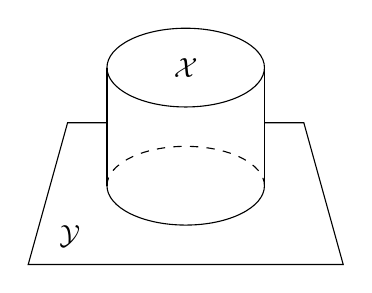
\begin{tikzpicture}[baseline=(O)]
	\draw (1, 1.5) ellipse[x radius=1, y radius=0.5] node {$\mathcal{X}$};
	\draw (0, 0) arc[start angle=180, end angle=360, x radius=1, y radius=0.5];
	\draw[dashed] (0, 0) arc[start angle=180, end angle=0, x radius=1, y radius=0.5];
	\draw (2, 1.5) -- (2, 0);
	\draw (0, 1.5) -- (0, 0);
	\draw (0, 0.8) -- (-0.5, 0.8) -- (-1, -1) node[xshift=1.5em,  yshift=1em] {$\mathcal{Y}$} -- (3, -1) -- (2.5, 0.8) -- (2, 0.8);
	\coordinate (O) at (0, 0.5);
\end{tikzpicture} \quad
	\Cone_{\mathrm{top}}(F) = 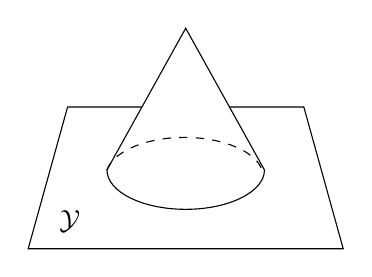
\begin{tikzpicture}[baseline=(O)]
	\draw (0, 0.8) -- (-0.5, 0.8) -- (-1, -1) node[xshift=1.5em,  yshift=1em] {$\mathcal{Y}$} -- (3, -1) -- (2.5, 0.8) --cycle;
	\filldraw[fill=white] (1, 1.8) -- (0, 0) arc[start angle=180, end angle=360, x radius=1, y radius=0.5] --cycle;
	\draw[dashed] (0, 0) arc[start angle=170, end angle=10, x radius=1, y radius=0.5];
	\coordinate (O) at (0, 0.5);
\end{tikzpicture}\]

单纯形集是剖析拓扑空间的一种具体手段. 稍加精确地说, 定理 \ref{prop:geom-Sing-adjunction} 给出伴随对
\[\begin{tikzcd}
	{|\cdot|}: \cate{sSet} \arrow[shift left, r] & \cate{Top}: \mathrm{Sing}, \arrow[shift left, l]
\end{tikzcd}\]
而且两端在某种精确意义下实现相互等价的同伦理论; 若以 $\cate{CGHaus}$ 代替 $\cate{Top}$, 前述构造同样适用. 我们现在着手将先前的讨论翻译到 $\cate{sSet}$ 中. 为此不妨就假定
\[ \mathcal{X} = |X|, \quad \mathcal{Y} = |Y|, \quad F = |f|: |X| \to |Y|, \]
其中 $f: X \to Y$ 是 $\cate{sSet}$ 的态射. 就单纯形集的立场, 映射锥比映射柱更容易解释. 我们先从 $\mathcal{X}$ 的锥 $\Cone_{\mathrm{top}}(\mathcal{X}) := \Cone_{\mathrm{top}}(\identity_{\mathcal{X}})$ 切入. 在 $\mathcal{X} = |X|$ 的前提下, $\Cone_{\mathrm{top}}(\mathcal{X}) \simeq |X^{\lhd}| \simeq |X^{\rhd}|$ (例 \ref{eg:cone-realization}). 以下将聚焦于 $X$ 的左锥 $X^{\lhd} = \Delta^0 \star X$ 和对应的链复形.
\index{danchunxingji!锥 (cone)}

对任意单纯形集 $Z$, 其中的非退化 $n$-单纯形构成集合 $Z^{\mathrm{nd}}_n$. 记 $\{\mathrm{pt}\} = (\Delta^0)_0 = (\Delta^0)^{\mathrm{nd}}_0$. 命题 \ref{prop:join-nd} 或拓扑直观表明
\begin{equation}\label{eqn:Cone-X-aux1}
	(\Delta^0 \star X)^{\mathrm{nd}}_n = \begin{cases}
		X^{\mathrm{nd}}_n \sqcup \left( \{ \mathrm{pt} \} \times X^{\mathrm{nd}}_{n-1} \right), & n > 0 \\
		\{\mathrm{pt}\} \sqcup X_0, & n = 0.
	\end{cases}
\end{equation}

代入 \eqref{eqn:join-formulas} 和其上讨论的一般公式, 可见当 $n \geq 1$ 时 $d_i: (\Delta^0 \star X)_n \to (\Delta^0 \star X)_{n-1}$ 在子集 $\{\mathrm{pt}\} \times X_{n-1}$ 和 $X_n$ 上的限制是
\begin{equation}\label{eqn:Cone-X-aux2}\begin{gathered}
	\begin{tikzcd}[column sep=small,
		/tikz/execute at end picture={
			\node [rectangle, draw, fit=(A) (B)] {};
			\node at ($(A)!.5!(C) + (0, 0.8)$) {$1 \leq i \leq n$};
		}]
		|[alias=A]| \{\mathrm{pt}\} \times X_{n-1} \arrow[d, "{\identity \times d_{i-1}}"'] & |[alias=C]| X_n \arrow[d, "{d_i}"] \\
		\{\mathrm{pt}\} \times X_{n-2} & |[alias=B]| X_{n-1}
	\end{tikzcd} \quad
	\begin{tikzcd}[column sep=small,
		/tikz/execute at end picture={
			\node [rectangle, draw, fit=(A) (B)] {};
			\node at ($(A)!.5!(C) + (0, 0.8)$) {$i=0$};
		}]
		|[alias=A]| \{\mathrm{pt}\} \times X_{n-1} \arrow[rd, "{\mathrm{pr}_2}"] & |[alias=C]| X_n \arrow[d, "{d_0}"] \\
		\{\mathrm{pt}\} \times X_{n-2} & |[alias=B]| X_{n-1}
	\end{tikzcd}
\end{gathered}\end{equation}
当 $n=1$ 时, 上式的 $\{\mathrm{pt}\} \times X_{n-2}$ 应理解为 $\{\mathrm{pt}\}$.

由于我们的目标是链复形, 下一步是将问题通过定义 \ref{def:free-simplicial-Ab} 的函子 $\Z(\cdot)$ 作线性化, 再以 Dold--Kan 对应过渡到链复形
\begin{equation*}
	\mathrm{N}(\Z X^{\lhd}) \simeq \mathrm{C}(\Z X^{\lhd}) \big/ \text{退化部分} \quad \text{(命题 \ref{prop:Dold-Kan-v})};
\end{equation*}
既然 $\mathrm{C}(\Z X^{\lhd})$ 的链复形结构来自 $\partial_n := \sum_{i=0}^n (-1)^i d_i$, 结合 \eqref{eqn:Cone-X-aux1}, \eqref{eqn:Cone-X-aux2} 连同注记 \ref{rem:cone-chain} 对 $\Cone(\identity_{\mathrm{N}X})$ 的描述, 可得链复形的短正合列
\[ 0 \to \underbracket{\Z\{\mathrm{pt}\}}_{\text{零次项}} \to \mathrm{N}(\Z X^{\lhd}) \to \Cone(\identity_{\mathrm{N}X}) \to 0. \]

其次, 函子 $|\cdot|$ 和 $\mathrm{N}$ 保推出图表, 这是因为它们分别是左伴随以及等价, 而推出图表在拓扑中的意义是黏合. 因此若对 $f: X \to Y$ 定义
\begin{equation*}
	\Cone_{\mathrm{s}}(f) := X^{\lhd} \dsqcup{X, f} Y,	
\end{equation*}
则有
\[\begin{tikzcd}
	\mathcal{X} \arrow[d, "F"'] \arrow[r, "{\text{底部}}"] & \Cone_{\mathrm{top}}(\mathcal{X}) \arrow[d] \\
	\mathcal{Y} \arrow[r] & \Cone_{\mathrm{top}}(F) \arrow[phantom, lu, "\boxplus" description]
\end{tikzcd} \xleftarrow{|\cdot|} \begin{tikzcd}
	X \arrow[d, "f"'] \arrow[r, "\text{典范}"] & X^{\lhd} \arrow[d] \\
	Y \arrow[r] & \Cone_{\mathrm{s}}(f) \arrow[phantom, lu, "\boxplus" description]
\end{tikzcd} \xrightarrow{\mathrm{N}} \begin{tikzcd}
	\mathrm{N}X \arrow[d, "{\mathrm{N}f}"'] \arrow[r] & \mathrm{N}X^{\lhd} \arrow[d] \\
	\mathrm{N}Y \arrow[r] & \mathrm{N}\Cone_{\mathrm{s}}(f) \arrow[phantom, lu, "\boxplus" description]
\end{tikzcd}\]
这一系列操作提示 $\Cone_{\mathrm{top}}(F)$ 的线性代数化身应当是 $\mathrm{N}\Cone_{\mathrm{s}}(f)$.

\begin{proposition}\label{prop:Cone-comparison}
	\index{yingshezhui}
	符号同上, 我们有链复形的典范短正合列
	\[ 0 \to \underbracket{\Z\{\mathrm{pt}\}}_{\text{零次项}} \to \mathrm{N}\Cone_{\mathrm{s}}(f) \to \Cone(\mathrm{N}f) \to 0. \]
\end{proposition}
\begin{proof}
	推出不触及 $\mathrm{N}X^{\lhd}$ 的子链复形 $\Z\{\mathrm{pt}\}$ (对应锥的顶点), 而它将 $n$ 次项的所有 $X_n$ 换成 $Y_n$, 并将 \eqref{eqn:Cone-X-aux2} 的投影 $\mathrm{pr}_2$ 换成 $f_{n-1} \mathrm{pr}_2$. 因此在商 $\Cone(\identity_{\mathrm{N}X})$ 的层次, 推出的产物无非是 $\Cone(\mathrm{N}f)$; 参阅注记 \ref{rem:cone-chain}.
\end{proof}

\begin{remark}
	映射柱 $\Cyl_{\mathrm{top}}(F)$ 及其链复形版本也可以作类似的会通, 而且此时不必再对顶点的贡献取商. 不过由于映射柱涉及单纯形集的乘积, 而 $\mathrm{N}$ 并非幺半函子, 所以拓扑学中一般是通过 CW 复形而非单纯形集来作解释, 乘积在 CW 复形的世界中更容易操作.
\end{remark}

综上, 链复形的映射锥是来自单纯形集 (或拓扑) 的映射锥对一份 $\Z$ 的商, 这份 $\Z$ 来自锥的顶点 $\mathrm{pt}$. 在链复形的研究中, 映射锥的主要意义是任何映射 $\phi: A \to B$ 都拓展为列:
\begin{equation}\label{eqn:cofiber-comparison-A}
	A \xrightarrow{\phi} B \to \Cone(\phi) \to A[-1] \xrightarrow{-f[-1]} B[-1] \to \cdots
\end{equation}

在拓扑情境下, 对应到 $\Cone(\phi) \to A[-1]$ 的映射是将 $\Cone_{\mathrm{top}}(F)$ 的底 $\mathcal{Y}$ 缩为一点, 收缩的产物记为 $S\mathcal{X}$; 这与 $\mathcal{Y}$ 无关 (见下图), 给出函子 $S$. 对应的映射列如
\begin{equation*}
	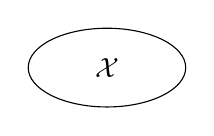
\begin{tikzpicture}[baseline=(O)]
		\draw (1, 0) ellipse[x radius=1, y radius=0.5] node {$\mathcal{X}$};
		\coordinate (O) at (0, 0);
	\end{tikzpicture}
	\xrightarrow{F}
	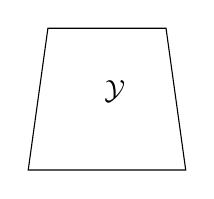
\begin{tikzpicture}[baseline=(O), xscale=0.5]
		\draw (0, 0.8) -- (-0.5, 0.8) -- (-1, -1) -- (3, -1) -- (2.5, 0.8) --cycle;
		\node at (1.2, 0) {$\mathcal{Y}$};
		\coordinate (O) at (0, 0.5);
	\end{tikzpicture}
	\xrightarrow{\text{嵌入}}
	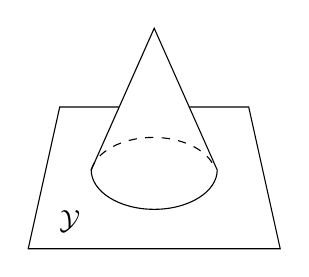
\begin{tikzpicture}[baseline=(O), xscale=0.8]
		\draw (0, 0.8) -- (-0.5, 0.8) -- (-1, -1) node[xshift=1.5em,  yshift=1em] {$\mathcal{Y}$} -- (3, -1) -- (2.5, 0.8) --cycle;
		\filldraw[fill=white] (1, 1.8) -- (0, 0) arc[start angle=180, end angle=360, x radius=1, y radius=0.5] --cycle;
		\draw[dashed] (0, 0) arc[start angle=170, end angle=10, x radius=1, y radius=0.5];
		\coordinate (O) at (0, 0.5);
	\end{tikzpicture}
	\xrightarrow{\text{缩}}
	\begin{tikzpicture}[baseline=(O), xscale=0.7, yscale=0.7]
		\draw (2, 0) -- (1, 1.8) -- (0, 0);
		\draw[dashed] (0, 0) arc[start angle=170, end angle=10, x radius=1, y radius=0.5];
		\draw (0, 0) arc[start angle=190, end angle=350, x radius=1, y radius=0.5];
		\node at (1, 0) {$\mathcal{X}$};
		\draw (0, 0) -- (1, -1.8) -- (2, 0);
		\coordinate (O) at (0, 0.5);
	\end{tikzpicture}
	\to \cdots
\end{equation*}
称之为 $f$ 生成的\emph{上纤维列} (精确地说, 不带基点的版本). 若在 $\cate{sSet}$ 中操作, 对相应的列取链复形, 得到的大致是 \eqref{eqn:cofiber-comparison-A}. 之所以说``大致'', 缘由在于:
\begin{itemize}
	\item 映射 $S\mathcal{X} \to S\mathcal{Y}$ 不能单纯地取为 $S(F)$, 而须适当地翻转垂直坐标, 这在线性代数的层次对应到 \eqref{eqn:cofiber-comparison-A} 中的 $-f[-1]$; 详见拓扑学相关教材.
	\item 如命题 \ref{prop:Cone-comparison} 所见, 各种链复形包含多余的 $\Z$, 对应到 $\Cone_{\mathrm{top}}(F)$ 和 $S\mathcal{X}$ 等空间的顶点. 拓扑学中摆脱这些问题的方式是考虑带基点的空间, 然后在锥的拓扑构造中缩掉和基点相连的部分.
\end{itemize}

倘若暂时略去一切细节, 大而化之地说, 则 \S\ref{sec:derived-cat} 建立的导出范畴理论 (取 $\mathcal{A} = \cate{Ab}$) 也可视为同伦论\footnote{应当说是稳定同伦论, 因为链复形容许有负次项.}的一种略为粗糙的``线性化''.

由于相关问题涉及愈来愈多的拓扑学思想和方法, 为免离题万里, 我们就此打住.

\begin{Exercises}
	\item 证明对于任何范畴 $\mathcal{C}$, 例 \ref{eg:const-simplicial} 的构造 $C \mapsto \mathrm{const}(C)$ 给出全忠实函子 $\mathcal{C} \to \cate{s}\mathcal{C}$.
	
	\item 设 $X$ 是单纯形集, $x \in X_n$. 证明存在数列 $j_1 < \cdots < j_h$ 和一个非退化单纯形 $y$ 使得 $x = s_{j_h} \cdots s_{j_1} (y)$, 而且 $y$ 唯一.
	
	\begin{hint}
		难点在唯一性. 设 $Sy = x = S' y'$, 其中 $S$ 和 $S'$ 都具有断言中的形式, 则可取一系列面态射的合成 $D$ 使得 $y = DS y = DS' y'$; 将 $DS'$ 转换成 $\tilde{S}'\tilde{D}$ 的形式 (符号不言自明), 则 $y$ 非退化蕴涵 $\tilde{S}' = \identity$, 故 $y' = \tilde{D}y$. 运用对称性来推导 $y = y'$ 和 $\tilde{D} = \identity$.
	\end{hint}
	
	\item 说明在 $\cate{sSet}$ 中有如下图表, 上下两半分别交换 ($0 \leq i < j \leq n$):
	\[\begin{tikzcd}
		\Delta^{n-2} \arrow[d, "{\iota_{i < j}}"'] \arrow[r, "{\mathrm{d}^{j-1}}"] & \Delta^{n-1} \arrow[d, "\iota_i"] \arrow[rd, "{\mathrm{d}^i}"] & \\
		\bigsqcup_{0 \leq i' < j' \leq n} \Delta^{n-2} \arrow[shift left, r] \arrow[shift right, r] & \bigsqcup_{i' = 0}^n \Delta^{n-1} \arrow[r] & \partial \Delta^n \\
		\Delta^{n-2} \arrow[u, "{\iota_{i < j}}"] \arrow[r, "{\mathrm{d}^i}"'] & \Delta^{n-1} \arrow[u, "\iota_j"'] \arrow[ru, "{\mathrm{d}^j}"'] &
	\end{tikzcd}\]
	其中 $\bigsqcup$ 是在 $\cate{sSet} = \cate{Set}^{\simpDelta^{\opp}}$ 中逐项取的, 而 $\iota_{i < j}$ (或 $\iota_i$) 意谓向第 $i < j$ (或第 $i$) 项的嵌入; 中段的各个箭头由此交换性刻画. 进一步说明中间段是余等化子.
	
	类似地, 说明对所有 $0 \leq k \leq n$ 也同样有
	\[\begin{tikzcd}
		\Delta^{n-2} \arrow[d, "{\iota_{i < j}}"'] \arrow[r, "{\mathrm{d}^{j-1}}"] & \Delta^{n-1} \arrow[d, "\iota_i"] \arrow[rd, "{\mathrm{d}^i}"] & \\
		\bigsqcup_{\substack{0 \leq i' < j' \leq n \\ i', j' \neq k}} \Delta^{n-2} \arrow[shift left, r] \arrow[shift right, r] & \bigsqcup_{\substack{0 \leq i' \leq n \\ i' \neq k}} \Delta^{n-1} \arrow[r] & \Lambda^n_k \\
		\Delta^{n-2} \arrow[u, "{\iota_{i < j}}"] \arrow[r, "{\mathrm{d}^i}"'] & \Delta^{n-1} \arrow[u, "\iota_j"'] \arrow[ru, "{\mathrm{d}^j}"'] &
	\end{tikzcd}\]
	其中间段是余等化子, 要求 $i, j \neq k$. 试说明这些余等化子的拓扑意涵.
	
	\item 验证定义 \ref{def:simplicial-join} 的统联运算 $\star$ 有以下性质.
	\begin{enumerate}[(i)]
		\item 单纯形集对 $\star$ 自然地成为幺半范畴, 以取常值 $\emptyset$ 的空单纯形集为幺对象.
		\item 注记 \ref{rem:simpDelta-order-reversal} 的倒序对偶性给出 $\cate{sSet}$ 的自同构, 暂且记为 $X \mapsto \hat{X}$. 说明 $(X \star Y)^{\wedge} \simeq \hat{Y} \star \hat{X}$.
		\item 验证 $\Delta^p \star \Delta^q \simeq \Delta^{p+q+1}$.
	\end{enumerate}

	\item 说明精确到典范同胚, 对单纯形集取倒序对偶不改变几何实现.
	\begin{hint}
		从 $\Delta^n$ 的情形起步.
	\end{hint}

	\item 验证例 \ref{eg:cone-realization} 的断言.

	\item 设 $\mathcal{C}$ 和 $\mathcal{C}'$ 为范畴. 定义范畴 $\mathcal{C} \star \mathcal{C}'$ 如下:
	\begin{align*}
		\Obj(\mathcal{C} \star \mathcal{C}') & := \Obj(\mathcal{C}) \sqcup \Obj(\mathcal{C}'), \\
		\Hom_{\mathcal{C} \star \mathcal{C}'}(X, Y) & := \begin{cases}
			\Hom_{\mathcal{C}}(X, Y), & X, Y \in \Obj(\mathcal{C}) \\
			\Hom_{\mathcal{C}'}(X, Y), & X, Y \in \Obj(\mathcal{C}'), \\
			\text{独点集}, & X \in \Obj(\mathcal{C}), \; Y \in \Obj(\mathcal{C}'), \\
			\emptyset, & X \in \Obj(\mathcal{C}'), \; Y \in \Obj(\mathcal{C}).
		\end{cases}
	\end{align*}
	态射的合成与恒等态射有自明的定义. 证明单纯形集的统联运算 $\star$ 和例 \ref{eg:nerve-cat} 的脉函子有以下关系
	\[ \mathrm{N}(\mathcal{C}) \star \mathrm{N}(\mathcal{C}') \simeq \mathrm{N}(\mathcal{C} \star \mathcal{C}'). \]

	\item 为等式 \eqref{eqn:shuffle-sign-0} 和 \eqref{eqn:shuffle-sign-1} 给出较为详细的证明.
	
	\item 对任意范畴中的单纯形对象 $X$, 定义称为移位的单纯形对象 $\mathrm{Déc}_0 X$ 和 $\mathrm{Déc}^0 X$ 使得 $(\mathrm{Déc}_0 X)_n = (\mathrm{Déc}^0 X)_n = X_{n+1}$,
	\begin{gather*}
		d^{\mathrm{Déc}_0 X, n}_i = d^{X, n+1}_i, \quad s^{\mathrm{Déc}_0 X, n}_j = s^{X, n+1}_j, \\
		d^{\mathrm{Déc}^0 X, n}_i = d^{X, n+1}_{i+1}, \quad
		s^{\mathrm{Déc}^0 X, n}_j = s^{X, n+1}_{j+1}.
	\end{gather*}
	说明这是良定义的, 两者通过倒序对偶相联系 (注记 \ref{rem:simpDelta-order-reversal}), 而且对于加性范畴有 $\mathrm{C}(\mathrm{Déc}^0 X) = \mathrm{C}(X)[1]$ (参阅注记 \ref{rem:chain-cplx-translation}).
	\index{danchunxingduixiang!移位 (décalage)}
	\index[sym1]{Dec@$\mathrm{Déc}_0 X, \mathrm{Déc}^0 X$}

	\item 承上题, 说明 $d_0: X_1 \to X_0$ (或 $d_1: X_1 \to X_0$) 使 $\mathrm{Déc}_0 X$ (或 $\mathrm{Déc}^0 X$) 增广, 以 $X_0$ 为其 $-1$ 次项. 进一步说明在增广之后 $\mathrm{Déc}_0 X$ 右可缩, $\mathrm{Déc}^0 X$ 左可缩; 见定义 \ref{def:contractible-aug}.
	\begin{hint}
		处理 $\mathrm{Déc}_0 X$ 即可. 取 $k_{n-1} := s_n: X_n \to X_{n+1}$.
	\end{hint}

	\item 证明小范畴 $\mathcal{C}$ 是广群 (定义: 所有态射皆可逆) 当且仅当 $\mathrm{N}\mathcal{C}$ 具有以下条件: 对所有 $n \in \Z_{\geq 0}$ 和 $0 \leq i \leq n$, 任何态射 $\Lambda^n_i \to \mathrm{N}\mathcal{C}$ 都可以延拓为 $\Delta^n \to \mathrm{N}\mathcal{C}$, 不要求唯一性; 满足此延拓条件的单纯形集称为 Kan 复形.

	\item 延续例 \ref{eg:classifying-space-std-cplx} 的讨论, 说明正规化复形 $\overline{\mathsf{L}}$ (翻转为链复形) 同构于 $\mathrm{N}(\Bbbk\mathrm{E}\Gamma)$.
	\begin{hint}
		先以命题 \ref{prop:Dold-Kan-v} 将 $\mathrm{N}(X)$ 等同于 $\mathrm{C}(X)$ 的商.
	\end{hint}
	
	\item 设 $\Gamma$ 为幺半群. 记 $\cated{Set}\Gamma$ 为全体右 $\Gamma$-小集形成的范畴.
	\begin{enumerate}[(i)]
		\item 明确描述自由--忘却伴随对
		\[\begin{tikzcd}
			\mathrm{F}: \cate{Set} \arrow[shift left, r] & \cated{Set}\Gamma \arrow[shift left, l]: U
		\end{tikzcd}\]
		和对应的单位态射和余单位态射. 说明对应的单子 $T$ 将 $\cated{Set}\Gamma$ 等同于 $\cate{Set}^T$.
		
		\begin{hint}
			函子 $\mathrm{F}$ 映集合 $X$ 为 $X \times \Gamma$, 其中 $\Gamma$ 以右乘作用于第二个分量. 单位态射是 $x \mapsto (x, 1)$ 而余单位是作用映射.
		\end{hint}
		\item 对每个右 $\Gamma$-集 $X$ 描述 $\cated{Set}\Gamma$ 中对应的单纯形对象 $\mathrm{Bar}(X)$ (例 \ref{eg:bar-adjunction}, 例 \ref{eg:bar-comonad}).
		\item 取独点集 $X = \{\mathrm{pt}\}$, 赋予平凡右 $\Gamma$-作用. 说明对应的单纯形对象同构于例 \ref{eg:classifying-space} 介绍的 $\mathrm{E}\Gamma$, 后者通过每个 $(\mathrm{E}\Gamma)_n$ 上的右 $\Gamma$-作用成为 $\cated{Set}\Gamma$ 中的单纯形对象.
	\end{enumerate}

	\item 选定群 $\Gamma$. 在例 \ref{eg:HH-comonad} 中取群代数 $R = \Bbbk[\Gamma]$, 取 $M$ 为平凡 $\Gamma$-模 $\Bbbk$ (例 \ref{eg:trivial-G-mod}). 说明对应的 $\epsilon_{\Bbbk}: \mathrm{C}(\mathrm{Bar}(\Bbbk)) \to \Bbbk$ 同构于命题 \ref{prop:trivial-mod-resolution} 的解消 $\mathsf{L} = (\mathsf{L}_n, \partial'_n)_n \to \Bbbk$.
	\begin{hint}
		应用 \eqref{eqn:L-basis-partial}.
	\end{hint}

	\item 取交换环 $\Bbbk$ 和 $\mathcal{A} = \Bbbk\dcate{Mod}$, $\otimes = \otimes_{\Bbbk}$. 设 $\Gamma$ 为群, 考虑例 \ref{eg:classifying-contractible} 中的单纯形对象 $\Bbbk\mathrm{E}\Gamma$, 在 Alexander--Whitney 映射的定义 \ref{def:Eilenberg-Zilber} 中代入 $X := \Bbbk\mathrm{E}\Gamma \boxtimes \Bbbk\mathrm{E}\Gamma$, 然后考虑态射
	\[ \mathrm{C}(\Bbbk\mathrm{E}\Gamma) \to \mathrm{C}(\underbracket{\Bbbk\mathrm{E}\Gamma \otimes \Bbbk\mathrm{E}\Gamma}_{\simeq \Bbbk(\mathrm{E}\Gamma \times \mathrm{E}\Gamma)}) \xrightarrow{\overline{\mathrm{AW}}} \mathrm{C}(\Bbbk\mathrm{E}\Gamma) \otimes \mathrm{C}(\Bbbk\mathrm{E}\Gamma), \]
	第一段由单纯形集的对角嵌入 $\mathrm{E}\Gamma \to \mathrm{E}\Gamma \times \mathrm{E}\Gamma$ 诱导; 鉴于例 \ref{eg:classifying-space-std-cplx}, 其合成也相当于链复形的态射
	\[ \mathsf{L} \to \mathsf{L} \otimes \mathsf{L}. \]
	试由此诠释定义群上同调的杯积时用过的态射 $\Delta: \mathsf{L} \to \mathsf{L} \otimes \mathsf{L}$; 见引理 \ref {prop:cup-resolution} (ii).
	
	\begin{hint}
		代入 $\overline{\mathrm{AW}}$ 的定义可见合成态射的 $(p, q)$ 分量和引理 \ref {prop:cup-resolution} (ii) 差一个 $(-1)^{pq}$. 差异缘于该处探讨的是 $(\mathsf{L}_n, \partial_n)_n$ 而例 \ref{eg:classifying-space-std-cplx} 则取 $(\mathsf{L}_n, \partial'_n)_n$. 两者在单纯形集 $\mathrm{E}\Gamma$ 的层次差一个倒序 (注记 \ref{rem:simpDelta-order-reversal}); 留意到倒序对偶性调换 $\lambda^n_p$ 和 $\rho^n_q$ 在 $\overline{\mathrm{AW}}$ 中的角色, 或者说是调换两份 $\mathrm{C}(\Bbbk\mathrm{E}\Gamma)$.
	\end{hint}

	\item 考虑范畴 $\mathcal{D}$ 上的余单子 $(L, \delta, \epsilon)$. 对任意 $\mathcal{M} \in \Obj(\mathcal{D})$, 若 $\epsilon_{\mathcal{M}}: L\mathcal{M} \to \mathcal{M}$ 有右逆 $f: \mathcal{M} \to L\mathcal{M}$, 则称 $\mathcal{M}$ 是 \emph{$L$-投射}对象. 对偶地, 从范畴 $\mathcal{C}$ 上的单子 $(T, \mu, \eta)$ 可定义何谓 $\mathcal{C}$ 的 \emph{$T$-内射}对象.
	
	基于对偶性, 以下主要讨论 $L$-投射的概念. 按照例 \ref{eg:monad-simplicial} 的方法在 $\End(\mathcal{D})$ 中得到增广单纯形对象 $(L^{n+1})_{n \geq -1}$ (符号中省略 $d_i$, $s_j$ 等资料). 给定 $L$-投射的 $\mathcal{M}$ 和相应的 $f$, 定义
	\[ k_n := L^{n+1} f : L^{n+1} \mathcal{M} \to L^{n+2} \mathcal{M}, \quad n \geq -1. \]
	证明这使增广单纯形对象 $(L^{n+1} \mathcal{M})_{n \geq -1}$ 右可缩 (定义 \ref{def:contractible-aug}).

	\begin{hint}
		已知 $\epsilon_{\mathcal{M}} k_{-1} = \epsilon_{\mathcal{M}} f = \identity_{\mathcal{M}}$, 两边同取 $L^{n+1}$ 给出 $d_{n+1} k_n = \identity_{X_n}$, 而函子性确保
		\[\begin{tikzcd}
			L\mathcal{M} \arrow[r, "Lf"] \arrow[d, "{\epsilon_{\mathcal{M}}}"'] & L^2 \mathcal{M} \arrow[d, "{\epsilon_{L\mathcal{M}}}"] \\
			\mathcal{M} \arrow[r, "f"'] & L\mathcal{M}
		\end{tikzcd} \quad\text{交换, 亦即}\; d_0 k_0 = 	f\epsilon_{\mathcal{M}} = k_{-1} \epsilon_{\mathcal{M}}; \]
		以 $L^{n-i}f$ 代 $f$, 再对相应的图表取 $L^i$, 同理可得 $d_i k_n = k_{n-1} d_i$ 对 $0 \leq i \leq n$ 成立.
	\end{hint}

	\item 对于环 $R$, 自由--忘却伴随对 $\cate{Set} \leftrightarrows R\dcate{Mod}$ 确定 $R\dcate{Mod}$ 上的余单子 $L$. 证明一个左 $R$-模是 $L$-投射的当且仅当它是投射模.

	\item 考虑伴随对
	$\begin{tikzcd}
		F: \mathcal{C} \arrow[shift left, r] & \mathcal{D}: G \arrow[shift left, l]
	\end{tikzcd}$
	和 $\End(\mathcal{D})$ 上相应的余单子 $(L, \delta, \epsilon) = (FG, F\eta G, \epsilon)$ (例 \ref{eg:adjunction-monad}). 证明形如 $F\mathcal{N}$ 的对象 ($\mathcal{N} \in \Obj(\mathcal{C})$) 总是 $L$-投射的. 作为推论, 对所有 $\mathcal{M} \in \Obj(\mathcal{D})$, 单纯形对象 $(L^{n+1} \mathcal{M})_{n \geq 0}$ 的每一项都是 $L$-投射对象.
	
	\begin{hint}
		取 $f = F\eta_{\mathcal{N}}: F(\mathcal{N}) \to FGF(\mathcal{N}) = L(F(\mathcal{N}))$, 则 $\epsilon_{F(\mathcal{N})} f = \identity_{F(\mathcal{N})}$ 不外是伴随对的标准性质.
	\end{hint}

	\item 仍考虑来自伴随对 $(F, G)$ 的余单子 $L$. 说明 $\mathcal{P} \in \Obj(\mathcal{D})$ 是 $L$-投射的当且仅当它有以下提升性质: 对 $\mathcal{D}$ 的任意态射 $\alpha: \mathcal{M}_1 \to \mathcal{M}_2$ 和 $\phi: \mathcal{P} \to \mathcal{M}_2$, 若 $G\alpha$ 有右逆, 则存在 $\beta: \mathcal{P} \to \mathcal{M}_1$ 使得 $\phi = \alpha\beta$.

	\begin{hint}
		对于``当''的方向, 对 $\alpha := \epsilon_{\mathcal{P}}: FG(\mathcal{P}) \to \mathcal{P}$ 和 $\phi := \identity$ 应用提升性质. 对于``仅当''方向, 首先解释在提升性质中可用 $FG(\mathcal{P})$ 代 $\mathcal{P}$, 然后以伴随性质说明 $\alpha_*: \Hom(FG(\mathcal{P}), \mathcal{M}_1) \to \Hom(FG(\mathcal{P}), \mathcal{M}_2)$ 满.
	\end{hint}

	\item 对任意交换环 $\Bbbk$ 和 $\Bbbk$-代数的同态 $S \to R$, 考虑伴随对
	\begin{equation*}\begin{tikzcd}[row sep=small]
		R \dotimes{S} (\cdot): S\dcate{Mod} \arrow[shift left, r] & R\dcate{Mod}: \text{忘却}, \arrow[shift left, l] \\
		\text{忘却}: R\dcate{Mod} \arrow[shift left, r] & S\dcate{Mod}: \Hom_S(R, \cdot) \arrow[shift left, l]
	\end{tikzcd}\end{equation*}
	由此分别得到 $R\dcate{Mod}$ 上的余单子 $L$ 和单子 $T$. 试以先前介绍的提升性质 (或其对偶) 给出一个左 $R$-模 $M$ 作为 $L$-投射 (或 $T$-内射) 对象的充要条件, 然后比较它和投射模 (或内射模) 的异同.
	
	在此基础上可以建立一套称为\emph{相对同调代数}的理论, 详见 \cite{Ho56}; 其特色是它仅考量在 $S$ 上分裂正合的 $R$-模正合列. 稍后的习题将探讨相对版本的 $\Tor$ 和 $\Ext$ 函子.
	\index{xiangduitongdiaodaishu@相对同调代数 (relative homological algebra)}

	\item 考虑 Abel 范畴之间的伴随对
	$\begin{tikzcd}
		F: \mathcal{C} \arrow[shift left, r] & \mathcal{D}: G \arrow[shift left, l]
	\end{tikzcd}$.
	对所有 $\mathcal{M} \in \Obj(\mathcal{D})$ 证明:
	\begin{enumerate}[(i)]
		\item 存在 $\cate{Ch}_{\geq 0}(\mathcal{D})$ 的对象 $\mathcal{P}_\bullet$ 连同态射 $\epsilon: \mathcal{P}_\bullet \to \mathcal{M}$, 使得
		\begin{compactitem}
			\item 每个 $\mathcal{P}_n$ 都是 $L$-投射的 ($n \geq 0$),
			\item $\cdots \to G\mathcal{P}_1 \to G\mathcal{P}_0 \to G\mathcal{M} \to 0$ 的恒等态射零伦 (换言之, 它是分裂正合复形).
		\end{compactitem}
		\begin{hint}
			应用命题 \ref{prop:bar-null-homotopic}.
		\end{hint}
		\item 给定任两组满足上述条件的态射 $\epsilon: \mathcal{P}_\bullet \to \mathcal{M}$ 和 $\epsilon': \mathcal{P}'_\bullet \to \mathcal{M}$, 存在同伦等价 $f: \mathcal{P} \to \mathcal{P}'$ 使得 $\epsilon' f = \epsilon$.
		\begin{hint}
			需要之前介绍的提升性质.
		\end{hint}
	\end{enumerate}

	\index{yudanzitongdiao@余单子同调 (cotriple homology)}
	\index{ganggouzao}
	\item (M.\ Barr, J.\ M.\ Beck) 设 $L$ 是范畴 $\mathcal{D}$ 上的余单子; 例 \ref{eg:monad-simplicial} 的构造在 $\mathcal{M} \in \Obj(\mathcal{D})$ 取值给出的单纯形对象记为 $\mathrm{Bar}(\mathcal{M})$. 对任意 Abel 范畴 $\mathcal{A}$ 和函子 $E: \mathcal{D} \to \mathcal{A}$, 定义 $(L, E)$ 的\emph{余单子同调}为 $\cate{Ch}_{\geq 0}(\mathcal{A})$ 的一族对象
	\[ \Hm^L_n(E; \mathcal{M}) := \Hm_n\left( \mathrm{C}(E\mathrm{Bar}(\mathcal{M})) \right), \quad n \in \Z_{\geq 0}, \]
	其中 $E\mathrm{Bar}(\mathcal{M})$ 代表对 $\mathrm{Bar}(\mathcal{M})$ 逐项地取 $E$. 对偶地, 若 $T$ 是范畴 $\mathcal{C}$ 上的单子, $F: \mathcal{C} \to \mathcal{A}$ 是映向 Abel 范畴的函子, 则同样能定义 $(T, F)$ 的\emph{单子上同调}在 $\mathcal{N} \in \Obj(\mathcal{C})$ 的取值, 不必赘言.

	\begin{enumerate}[(i)]
		\item 写下自然态射 $\Hm^L_0(E; \mathcal{M}) \to E\mathcal{M}$, 说明当 $\mathcal{M}$ 为 $L$-投射对象时此为同构.
		\item 设 $L$ 来自 Abel 范畴之间的伴随对 $(F, G)$, 而 $E$ 是加性函子. 证明若 $\mathcal{P}_\bullet \to \mathcal{M}$ 是 $\cate{Ch}_{\geq 0}(\mathcal{D})$ 的态射, 满足
		\begin{compactitem}
			\item 每个 $\mathcal{P}_n$ 都是 $L$-投射的 ($n \geq 0$),
			\item $\cdots \to G\mathcal{P}_1 \to G\mathcal{P}_0 \to G\mathcal{M} \to 0$ 的恒等态射零伦,
		\end{compactitem}
		则 $\Hm^L_n(E; \mathcal{M}) \simeq \Hm_n(E\mathcal{P}_\bullet)$. 因此, 余单子同调可以用合适的 $L$-投射解消来计算.
		\item 承继先前假设. 若 $\mathcal{D}$ 的态射 $\mathcal{M}' \to \mathcal{M} \to \mathcal{M}''$ 取 $G$ 之后是 $\mathcal{C}$ 的分裂短正合列, 则称之为 $G$-分裂短正合列. 证明 $G$-分裂短正合列自然地诱导 $\Hm^L_n(E; \cdot)$ 的长正合列.
	\end{enumerate}

	\index{Ext hanzi!相对 (relative)}
	\index{Tor hanzi!相对 (relative)}
	\item (G.\ Hochschild \cite{Ho56}) 对任意交换环 $\Bbbk$ 和 $\Bbbk$-代数的同态 $S \to R$, 考虑伴随对
	\[\begin{tikzcd}
		R \dotimes{S} (\cdot): S\dcate{Mod} \arrow[shift left, r] & R\dcate{Mod}: \text{忘却} \arrow[shift left, l]
	\end{tikzcd}\]
	在 $R\dcate{Mod}$ 上确定的余单子 $L$. 对右 $R$-模 $A$ 和左 $R$-模 $B$, $N$, 定义 $\Bbbk$-模
	\begin{align*}
		\Tor^{R|S}_n(A, N) & := \Hm^L_n\left( A \dotimes{R}(\cdot) ; N \right), \\
		\Ext_{R|S}^n(N, B) & := \Hm^L_n\left( \Hom_R(\cdot, B) ; N \right),
	\end{align*}
	此处 $\Hom_R(\cdot, B)$ 视为函子 $R\dcate{Mod} \to S\dcate{Mod}^{\opp}$. 它们称为相对 $\Tor$ 和相对 $\Ext$ 函子.
	\begin{enumerate}[(i)]
		\item 说明两者对每个变元皆有函子性. 试明确相应的链复形, 并说明
		\[ \Tor^{R|S}_0(A, N) \simeq A \dotimes{R} N, \quad \Ext_{R|S}^0(N, B) \simeq \Hom_R(N, B). \]
		
		\item 说明双函子 $\Tor^{R|S}_n$ 有类似于定理 \ref{prop:balanced-primer} 的``平衡''性质.\footnote{避谈 $\Ext_{R|S}^n$ 是因为它涉及单子上同调的概念, 此处不细说, 详阅参考文献.}
		
		\item 证明若 $I$ 是 $S$ 的双边理想而 $R = S/I$, 则当 $n > 0$ 时 $\Tor_n^{R|S} = 0 = \Ext^n_{R|S}$. 由此可见相对 $\Tor$ 和相对 $\Ext$ 不同于 \S\ref{sec:Ext-Tor} 的绝对版本.
		\begin{hint}
			此时 $L = \identity_{R\dcate{Mod}}$.
		\end{hint}
		
		\item 记 $R^e = R \dotimes{\Bbbk} R^{\opp}$. 证明 $\HHm_n(M) \simeq \Tor^{R^e|\Bbbk}_n(M, R)$ 而 $\HHm^n(M) \simeq \Ext_{R^e|\Bbbk}^n(R, M)$; 参见例 \ref{eg:HH-comonad}.
		\begin{hint}
			归结为说明 $\mathrm{C}(\mathrm{Bar}(R))_n = R \otimes R^{\otimes n} \otimes R$ 是 $L$-投射的 $R^e$-模.
		\end{hint}
	\end{enumerate}
\end{Exercises}
	% LaTeX source for book ``代数学方法'' in Chinese
% Copyright 2024  李文威 (Wen-Wei Li).
% Permission is granted to copy, distribute and/or modify this
% document under the terms of the Creative Commons
% Attribution 4.0 International (CC BY 4.0)
% http://creativecommons.org/licenses/by/4.0/

% To be included
\chapter{对偶性}\label{sec:duality}
对偶性的概念起源于向量空间理论. 选定域 $\Bbbk$, 记 $\Bbbk$-向量空间 $V$ 的对偶空间为 $V^\vee := \Hom_{\Bbbk}(V, \Bbbk)$, 则有
\begin{itemize}
	\item 求值映射 $\mathrm{ev}: V \otimes V^\vee \to \Bbbk$, 映 $v \otimes \lambda$ 为 $\lambda(v)$;
	\item 当 $V$ 有限维时还有余求值映射 $\mathrm{coev}: \Bbbk \to V^\vee \otimes V$, 它映 $1$ 为 $\sum_{i=1}^n \check{v}_i \otimes v_i$, 其中 $(v_i)_{i=1}^n$ 是 $V$ 的任意基而 $(\check{v}_i)_{i=1}^n$ 是对偶基.
\end{itemize}
在有限维情形, 两者满足基本等式
\[ (\identity_{V^\vee} \otimes \mathrm{ev})(\mathrm{coev} \otimes \identity_{V^\vee}) = \identity_{V^\vee}, \quad (\mathrm{ev} \otimes \identity_V) (\identity_V \otimes \mathrm{coev}) = \identity_V. \]

在一般的幺半范畴中, \S\ref{sec:monoidal-dual} 定义的对偶资料是上述情景的直接推广: 这是一对对象 $(L, R)$ 连同态射 $\mathrm{ev}: L \otimes R \to \munit$ 和 $\mathrm{coev}: \munit \to R \otimes L$, 服从于上述基本等式; 此时称 $R$ 是 $L$ 的右对偶, $L$ 是 $R$ 的左对偶. 一切对象皆有左 (或右) 对偶的幺半范畴称为左 (或右) 刚性的.

对于辫幺半范畴, \S\ref{sec:symm-monoidal-dual} 将说明如何联系左右两种对偶, 从而在对象 $X$ 有对偶的前提下对 $f \in \End(X)$ 定义迹 $\Tr(f)$, 从而定义维数 $\dim X := \Tr(\identity_X)$, 它们都是 $\End(\munit)$ 的元素, 严格来说分为左右两种版本, 但是在对称幺半范畴中不必区别. 本书主要关注具有对称幺半结构的 Abel 范畴, 譬如交换环上的模范畴 (见命题 \ref{prop:dualizable-module}); 只要读者明白对偶向量空间的用处, 自能体会推广后的妙用; 对偶性在 $2$-范畴的框架下能发挥更大威力, 但这不属于本书范围.

对偶性的实例是 \S\ref{sec:duality-examples} 的主题, 其中和代数学最亲近的是 Hopf $\Bbbk$-代数 $A$ 上的有限维右 $A$-模范畴 $\catesubd{Mod}{\mathrm{f}}A$ 及其余模版本 $\catesubd{Comod}{\mathrm{f}}A$ (命题 \ref{prop:Hopf-module-dual}); 无论哪种情形, 对偶性都反映对极 $S: A \to A$ 的性质. Hopf 代数的例子对于量子群的研究尤其重要, 同时又是淡中范畴理论的预备知识.

本章 \S\S\ref{sec:coend}---\ref{sec:Hopf-reconstruction} 的内容涉及余代数的重构问题. 对任何余代数 $L$, Abel 范畴 $\catesubd{Comod}{\mathrm{f}}L$ 都是局部有限的 (定义 \ref{def:locally-finite}), 并带有忠实正合的忘却函子 $U: \catesubd{Comod}{\mathrm{f}}L \to \cate{Vect}_{\mathrm{f}}(\Bbbk)$. 重构问题关切的是反方向:
\begin{center}\begin{minipage}{0.8\textwidth}
	如何从局部有限 $\Bbbk$-线性 Abel 范畴 $\mathcal{A}$ 和忠实正合函子 $\omega: \mathcal{A} \to \cate{Vect}_{\mathrm{f}}(\Bbbk)$ 构造余代数 $L$, 使得 $(\mathcal{A}, \omega)$ 自然地等价于 $(\catesubd{Comod}{\mathrm{f}}L, U)$?
\end{minipage}\end{center}
本章的方案将涉及函子 $\omega$ 的自同态余代数 $\coEnd(\omega) = \coEnd_{\Bbbk}(\omega)$ (定义--命题 \ref{def:cogebra-L}), 它余作用在每个 $\omega(X)$ 上, 而且对此是``泛''的.

余代数重构定理 \ref{prop:Tannaka-aux1} 的证明涉及了 \S\ref{sec:Beck} 的余单子理论, \S\ref{sec:Morita} 关于森田理论的基本知识, \S\ref{sec:locally-finite-Abel-cat} 关于局部有限 Abel 范畴的技术性结果, 以及 \S\ref{sec:Indization-functor} 介绍的 Ind 化. 当 $(\mathcal{A}, \omega)$ 带有幺半结构时, $\coEnd(\omega)$ 相应地成为双代数. 若 $\mathcal{A}$ 既是左刚性又是右刚性的, 则 $\coEnd(\omega)$ 还是 Hopf 代数 (定理 \ref{prop:Tannaka-aux2}). 这部分的处理方式主要参照 \cite{Del90}.

在这一系列准备后, \S\ref{sec:Tannakian-cat} 将引入淡中范畴的严格定义. 这是一类具有特殊性质的对称幺半范畴 $\mathcal{T}$, 其形式定义来自 N.\ Saavedra Rivano 和 P.\ Deligne, 动机则可上溯至淡中忠郎等人的工作. 在定义 \ref{def:Tannakian-cat} 的诸多条件中, 最突出的是要求有非零交换 $\Bbbk$-代数 $B$ 和兼容于辫结构的右正合幺半函子 $\omega: \mathcal{T} \to \cated{Mod}B$, 称为 $\mathcal{T}$ 在 $B$ 上的纤维函子.

代数几何的场景要求容许一般的 $B$, 但许多初等应用只涉及中性纤维函子, 此时 $\omega$ 是取值在 $\cate{Vect}_{\mathrm{f}}(\Bbbk)$ 的忠实正合函子; 相应的淡中重构定理 \ref{prop:Tannaka-neutral} 不外是先前结果的应用, 它蕴涵 $\coEnd(\omega)$ 是交换 Hopf 代数, 并且将 $(\mathcal{T}, \omega)$ 等同于 $(\coEnd(\omega), U)$. 关于 $(\mathcal{T}, \omega)$ 的许多属性按此转译为 Hopf 代数的性质.

对于一般的纤维函子, 推论 \ref{prop:Aut-Tannakian} 将 $B$ 上的交换 Hopf 代数 $\coEnd_B(\omega)$ 和 $\omega$ 的 $\otimes$-自同构群 $\Aut^{\otimes}(\omega)$ 联系起来. 关于 $\coEnd_B(\omega)$ 的全部信息都蕴藏于 $\Aut^{\otimes}$, 前提是将后者理解为群函子 $B\dcate{CAlg} \to \cate{Grp}$, 而不只是单一的群. 这种见地在代数几何中浑然天成.

最后, \S\ref{sec:TK} 返回淡中范畴的历史渊源, 基于先前理论来说明给定有限群 $G$ 和域 $\Bbbk$, 如何从有限维 $G$-模范畴 $G\dcate{Mod}_{\mathrm{f}}$ (定义 \ref{def:G-mod}) 连同映向 $\cate{Vect}_{\mathrm{f}}(\Bbbk)$ 的忘却函子 $\omega$ 来重构群 $G$; 由于 $G\dcate{Mod}_{\mathrm{f}}$ 在抽象调和分析的语境下近乎 $G$ 的某种``对偶'', 故此结果也称为淡中--Krein 对偶定理的有限群版本. 事实上, 一旦知悉 $G$-模和函数空间 $C(G)$ 上的右余模是一回事, 则所求同构 $G \rightiso \Aut^{\otimes}(\omega)$ 有更短的证明, 绕道重构定理不过是为了阐明淡中范畴的来由.

\begin{wenxintishi}
	涉及 Hopf 代数的内容以及 \S\ref{sec:Tannaka-coend} 关于重构定理的证明都基于\CHref{sec:monads}的部分内容. 此外, 重构定理的证明还引用附录部分的 \S\ref{sec:locally-finite-Abel-cat} 和 \S\ref{sec:Indization-functor}, 初看时不必深究. 最后的 \S\ref{sec:TK} 涉及 $G$-模的基本概念, 详见 \S\ref{sec:G-mod} 前半部, 其后半部关于解消的讨论则与本章无关.
\end{wenxintishi}

\section{幺半范畴中的对偶性}\label{sec:monoidal-dual}
首先介绍适用于所有幺半范畴的一则概念, 然后渐次细化.

\begin{definition}\label{def:dualizable-obj}
	\index{duiou@对偶 (dual)}
	\index[sym1]{ev-coev}
	设 $\mathcal{C}$ 为幺半范畴, $L, R \in \Obj(\mathcal{C})$. 若存在态射
	\[ \mathrm{ev}: L \otimes R \to \munit, \quad \mathrm{coev}: \munit \to R \otimes L \]
	使得以下合成分别是 $\identity_R$ 和 $\identity_L$, 则我们称 $L$ 是 $R$ 的\emph{左对偶}, 称 $R$ 是 $L$ 的\emph{右对偶}:
	\begin{gather*}
		R \simeq \munit \otimes R \xrightarrow{\mathrm{coev} \otimes \identity_R} (R \otimes L) \otimes R \simeq  R \otimes (L \otimes R) \xrightarrow{\identity_R \otimes \mathrm{ev}} R \otimes \munit \simeq R, \\
		L \simeq L \otimes \munit \xrightarrow{\identity_L \otimes \mathrm{coev}} L \otimes (R \otimes L) \simeq (L \otimes R) \otimes L \xrightarrow{\mathrm{ev} \otimes \identity_L} \munit \otimes L \simeq L.
	\end{gather*}
	如上的 $(L, R, \mathrm{ev}, \mathrm{coev})$ 称为对偶资料.
\end{definition}

对偶资料中的 $\mathrm{ev}$ 和 $\mathrm{coev}$ 应当理解为``求值''态射及其对偶. 定义中涉及的幺元约束, 结合约束与括号顺序不会造成任何困难, 今后经常省略.

读者兴许会从定义 \ref{def:dualizable-obj} 联想到伴随函子的单位和余单位态射. 对偶性确实能涵摄伴随函子理论, 但这需要在 $2$-范畴或更广义的结构中进行操作, 不属本书范围.

\begin{proposition}\label{prop:monoidal-functor-dual}
	设 $F: \mathcal{C} \to \mathcal{D}$ 为幺半范畴之间的幺半函子, 则 $\mathcal{C}$ 的任何对偶资料 $(L, R, \mathrm{ev}, \mathrm{coev})$ 皆典范地诱导 $\mathcal{D}$ 的对偶资料 $(FL, FR, F\mathrm{ev}, F\mathrm{coev})$.
\end{proposition}
\begin{proof}
	为了将 $(FL, FR, F\mathrm{ev}, F\mathrm{coev})$ 诠释为对偶资料, 仅须考虑交换图表
	\[\begin{tikzcd}
		FL \otimes FR \arrow[r] & \munit_{\mathcal{D}} \arrow[r] & FR \otimes FL \\
		F(L \otimes R) \arrow[r, "{F\mathrm{ev}}"'] \arrow[u, "\sim" sloped] & F(\munit_{\mathcal{C}}) \arrow[u, "\sim" sloped] \arrow[r, "{F\mathrm{coev}}"'] & F(R \otimes L) \arrow[u, "\sim"' sloped]
	\end{tikzcd}\]
	垂直箭头来自幺半函子的结构. 所需性质依此化到 $\mathcal{C}$ 上.
\end{proof}

\begin{definition-proposition}\label{def:dual-uniqueness}
	\index[sym1]{Xstar@$X^*, {}^* X$}
	设 $\mathcal{C}$ 为幺半范畴, $X \in \Obj(\mathcal{C})$, 若 $X$ 有右对偶 (或左对偶), 对偶资料写作 $(X, X^*, \mathrm{ev}, \mathrm{coev})$ (或 $({}^* X, X, \mathrm{ev}, \mathrm{coev})$), 则这些资料精确到唯一同构是唯一的.
	
	有鉴于此, 我们可以合理地谈论 $X$ 的右对偶 $X^*$ (或左对偶 ${}^* X$) 而不致混淆.
\end{definition-proposition}
\begin{proof}
	调换 $\otimes$ 顺序即可在左和右对偶之间过渡, 故以下仅伦 $X^*$ 情形. 设资料 $(X_i^*, \mathrm{ev}_i, \mathrm{coev}_i)$ 给出 $X$ 的右对偶 ($i = 1, 2$). 首先论证同构的唯一性. 设 $\alpha: X_1^* \rightiso X_2^*$ 与对偶性的态射 $\mathrm{ev}_i$, $\mathrm{coev}_i$ 兼容, 则有交换图表
	\[\begin{tikzcd}[row sep=tiny]
		X_1^* \arrow[dd, "\alpha"'] \arrow[r, "{\mathrm{coev}_2 \otimes \identity}" inner sep=0.6em] & X_2^* \otimes X \otimes X_1^* \arrow[dd, "{\identity \otimes \alpha}"] \arrow[rd, "{\identity \otimes \mathrm{ev}_1}"] & \\
		& & X_2^* \\
		X_2^* \arrow[r, "{\mathrm{coev}_2 \otimes \identity}"' inner sep=0.6em] & X_2^* \otimes X \otimes X_2^* \arrow[ru, "{\identity \otimes \mathrm{ev}_2}"'] &
	\end{tikzcd}\]
	根据右对偶的定义, 其下路合成为 $(\identity \otimes \mathrm{ev}_2) (\mathrm{coev}_2 \otimes \identity) = \identity_{X_2^*}$; 对于逆态射 $\beta: X_2^* \rightiso X_1^*$ 也有相应的陈述. 因此所求的 $\alpha: X_1^* \to X_2^*$ 和 $\beta: X_2^* \to X_1^*$ 只能分别取作合成
	\begin{gather*}
		X_1^* \xrightarrow{\mathrm{coev}_2 \otimes \identity_{X_1^*}} X_2^* \otimes X \otimes X_1^* \xrightarrow{\identity_{X_2^*} \otimes \mathrm{ev}_1} X_2^* , \\
		X_2^* \xrightarrow{\mathrm{coev}_1 \otimes \identity_{X_2^*}} X_1^* \otimes X \otimes X_2^* \xrightarrow{\identity_{X_1^*} \otimes \mathrm{ev}_2} X_1^* .
	\end{gather*}
	
	兹断言以上定义的 $\alpha$ 和 $\beta$ 确实与对偶性的态射兼容. 基于对称性, 考虑 $\alpha$ 即可. 右对偶的定义给出交换图表
	\[\begin{tikzcd}
		X \otimes X_1^* \arrow[rd, "{\identity}"] \arrow[d, "{\identity \otimes \mathrm{coev}_2 \otimes \identity}"'] & \\
		X \otimes X_2^* \otimes X \otimes X_1^* \arrow[r, "{\mathrm{ev}_2 \otimes \identity}"' inner sep=0.6em] \arrow[d, "{\identity \otimes \mathrm{ev}_1}"'] & X \otimes X_1^* \arrow[d, "{\mathrm{ev}_1}"] \\
		X \otimes X_2^* \arrow[r, "{\mathrm{ev}_2}"'] & \munit
	\end{tikzcd} \quad \begin{tikzcd}
		\munit \arrow[r, "{\mathrm{coev}_1}"] \arrow[d, "{\mathrm{coev}_2}"'] & X_1^* \otimes X \arrow[d, "{\mathrm{coev}_2 \otimes \identity}"] \\
		X_2^* \otimes X \arrow[r, "{\identity \otimes \mathrm{coev}_1}" inner sep=0.6em] \arrow[rd, "{\identity}"'] & X_2^* \otimes X \otimes X_1^* \otimes X \arrow[d, "{\identity \otimes \mathrm{ev}_1 \otimes \identity}"] \\
		& X_2^* \otimes X
	\end{tikzcd}\]
	垂直方向的合成分别是 $\identity \otimes \alpha$ 和 $\alpha \otimes \identity$, 兼容性得证.
	
	其次证明 $\alpha$ 和 $\beta$ 互逆. 同理, 证 $\beta\alpha = \identity$ 即可. 考虑图表
	\[\begin{tikzcd}[column sep=large]
		X_1^* \arrow[d, "{\mathrm{coev}_2 \otimes \identity}"'] \arrow[r, "{\mathrm{coev}_1 \otimes \identity}"] & X_1^* \otimes X \otimes X_1^* \arrow[d, "{\identity \otimes \identity \otimes \mathrm{coev}_2 \otimes \identity}"'] \arrow[rd, "\identity"] & \\
		X_2^* \otimes X \otimes X_1^* \arrow[r, "{\mathrm{coev}_1 \otimes \identity}"'] \arrow[d, "{\identity \otimes \mathrm{ev}_1}"'] & X_1^* \otimes X \otimes X_2^* \otimes X \otimes X_1^* \arrow[d, "{\identity \otimes \mathrm{ev}_1}"'] \arrow[r, "{\identity \otimes \mathrm{ev}_2 \otimes \identity \otimes \identity}"' inner sep=0.6em] &  X_1^* \otimes X \otimes X_1^* \arrow[d, "{\identity \otimes \mathrm{ev}_1}"] \\
		X_2^* \arrow[r, "{\mathrm{coev}_1 \otimes \identity}"'] & X_1^* \otimes X \otimes X_2^* \arrow[r, "{\identity \otimes \mathrm{ev}_2}"'] & X_1^*
	\end{tikzcd}\]
	三个方块显然交换, 三角部分基于右对偶的定义交换, 故全图交换. 按
	$\begin{tikzpicture}[baseline=(O), scale=0.45]
		\coordinate (O) at (0, 0.5);
		\draw[->] (0, 1) -- (0, 0) -- (1, 0);
	\end{tikzpicture}$
	合成给出 $\beta\alpha$, 而按
	$\begin{tikzpicture}[baseline=(O), scale=0.45]
		\coordinate (O) at (0, 0.5);
		\draw[->] (0, 1) -- (1, 1) -- (1.5, 0.5) -- (1.5, 0);
	\end{tikzpicture}$
	合成则给出 $\identity_{X_1^*}$. 明所欲证.
\end{proof}

左对偶和右对偶的相互关系可表作 ${}^* (X^*) = X$ 和 $({}^* X)^* = X$. 尽管在论证或叙述中经常会选定对偶资料, 但对偶性究其实质乃是对象具有的一则性质, 而非外加的结构.

\begin{example}
	在任意幺半范畴中皆有
	\[ \munit^* = \munit = {}^* \munit, \]
	所需的态射 $\mathrm{ev}$ 和 $\mathrm{coev}$ 皆来自幺元约束 $\munit \otimes \munit \simeq \munit$.
\end{example}

\begin{definition}[N.\ Saavedra Rivano]\label{def:rigid-cat}
	\index{yaobanfanchou!刚性 (rigid)}
	若幺半范畴 $\mathcal{C}$ 的所有对象都有左对偶 (或右对偶), 则称 $\mathcal{C}$ 为\emph{左刚性} (或\emph{右刚性}) 范畴.
\end{definition}

\index{xiantu@线图 (string diagram)}
定义--命题 \ref{def:dual-uniqueness} 的证明思路简则简矣, 过程中却引进繁多的公式和交换图表. 在涉及对偶性的各种论证中, 称为\emph{线图}的可视化技巧十分方便; 参照 \S\ref{sec:alg-in-monoidal-cat} 或 \cite[定理 2.6.12 证明]{Li1}. 详言之, 我们以对象为节点, 态射为箭头, 由上而下地合成; 譬如 $\identity_X$, $f: X \to Y$, $g: Y \to Z$ 和 $gf$ 分别表为
\begin{center}\begin{tikzpicture}[morphism/.style={rectangle, draw, fill=white}]
		\node (A) {$X$};
		\node (B) [below=of A] {$X$};
		\path (A) edge (B);
		
		\node (X) [right=of A] {$X$};
		\node (Y) [below=of X] {$Y$};
		\path (X) edge[->] node[midway, morphism] {$f$} (Y);
		
		\node (Y2) [right=of X] {$Y$};
		\node (Z) [right=of Y] {$Z$};
		\path (Y2) edge[->] node[midway, morphism] {$g$} (Z);
		
		\node (X2) [right=of Y2] {$X$};
		\node (Z2) [below=2cm of X2] {$Z$};
		\path (X2) edge[->] node[near start, morphism] {$f$} node[near end, morphism] {$g$} (Z2);
\end{tikzpicture}\end{center}
因此将态射从前或后边合成 $\identity$ 相当于将箭头拉长. 对态射取 $\otimes$ 则表作箭头的并列, 譬如 $f \otimes g$ 表作
\begin{center}\begin{tikzpicture}[morphism/.style={rectangle, draw, fill=white}]
		\node (X) {$X$};
		\node (Y) [right=0.1cm of X] {$Y$};
		\node (Y1) [below=of X] {$Y$};
		\node (Z) [below=of Y] {$Z$};
		\path (X) edge[->] node[midway, morphism] {$f$} (Y1);
		\path (Y) edge[->] node[midway, morphism] {$g$} (Z);
\end{tikzpicture}\end{center}

由于 $X \otimes \munit \simeq X \simeq \munit \otimes X$, 在线图中可以合理地省略 $\munit$, 或者说箭头在该处无端点, 于是在对偶存在的前提下, $\mathrm{ev}: X \otimes X^* \to \munit$ 和 $\mathrm{coev}: \munit \to X^* \otimes X$ 便分别表作
\begin{center}\begin{tikzpicture}[bend angle=70, auto]
		\node (L) {$X$};
		\node (R) [right=of L] {$X^*$};
		\path (L) edge[bend right] node[midway] {$\mathrm{ev}$} (R);
		
		\node (LL) [right=of R] {$X^*$};
		\node (RR) [right=of LL] {$X$};
		\path (LL) edge[bend left] node[midway] {$\mathrm{coev}$} (RR);
\end{tikzpicture}\end{center}

相同前提下, 定义 \ref{def:dualizable-obj} 的等式
\[ (\identity_X \otimes \mathrm{ev}) (\mathrm{coev} \otimes \identity_X ) = \identity_X = (\mathrm{ev} \otimes \identity_X) (\identity_X \otimes \mathrm{coev}) \]
按此图解为
\begin{equation}\label{eqn:Zorro}
	\begin{tikzpicture}[baseline=(B), bend angle=70, auto]
		\node (A) {$X$};
		\node (B) [below=of A] {$X$};
		\node (C) [left=of B] {${}^* X$};
		\node (D) [left=of C] {$X$};
		\node (E) [below=of D] {$X$};
		
		\path (A) edge (B);
		\path (D) edge[bend left] node {$\mathrm{coev}$} (C);
		\path (C) edge[bend right] node {$\mathrm{ev}$} (B);
		
		\path (D) edge[->] (E);
	\end{tikzpicture} \quad = \quad
	\begin{tikzpicture}[baseline=(M)]
		\node (A) {$X$};
		\node (M) [below=of A] {};
		\node (B) [below=of M] {$X$};
		\path (A) edge (B);
		\coordinate (M) at ($(A)!.5!(B)$);
	\end{tikzpicture} \quad = \quad
	\begin{tikzpicture}[baseline=(B), bend angle=70, auto]
		\node (A) {$X$};
		\node (B) [below=of A] {$X$};
		\node (C) [right=of B] {$X^*$};
		\node (D) [right=of C] {$X$};
		\node (E) [below=of D] {$X$};
		
		\path (A) edge (B);
		\path (C) edge[bend left] node {$\mathrm{coev}$} (D);
		\path (B) edge[bend right] node {$\mathrm{ev}$} (C);
		
		\path (D) edge[->] (E);
	\end{tikzpicture}
\end{equation}
前提是所论的对偶存在; 这就赋予定义 \ref{def:dualizable-obj} 一种``拉直箭头''的操作感. 在一些文献中, 上述图表是旋转 $\frac{\pi}{2}$ 后描绘的, 因之又称 \emph{Z 字等式}.
\index{Z-zidengshi@Z 字等式 (mark of Zorro)}

基于代数等式和线图操作之间的这些对应, 涉及对偶性的基本代数等式容易按图索骥, 或者索性以图为证. 作为练习, 读者不妨尝试将定义--命题 \ref{def:dual-uniqueness} 的证明改写成简单的图表.

下一则结果说明对偶自然地调换 $\otimes$ 的次序.

\begin{proposition}
	设 $\mathcal{C}$ 为幺半范畴, $X, Y \in \Obj(\mathcal{C})$.
	\begin{enumerate}[(i)]
		\item 若 $X$ 和 $Y$ 分别有左对偶 ${}^* X$ 和 ${}^* Y$, 则 ${}^* Y \otimes {}^* X$ 给出 $X \otimes Y$ 的左对偶, 相应的资料可以通过 $X$ 和 $Y$ 的对偶资料图解为
		\begin{equation*}
			\mathrm{ev}_{X \otimes Y} = \left[ \begin{tikzcd}[column sep=tiny, ampersand replacement=\&]
				{}^* Y \arrow[dash, rrr, bend right=80, "{\mathrm{ev}_Y}"' near end] \& {}^* X \arrow[dash, r, bend right=60, "{\mathrm{ev}_X}"' near start] \& X \& Y
			\end{tikzcd}\right], \quad
			\mathrm{coev}_{X \otimes Y} = \left[ \begin{tikzcd}[column sep=tiny, ampersand replacement=\&]
				X \arrow[dash, rrr, bend left=80, "{\mathrm{coev}_X}" near start] \& Y \arrow[dash, r, bend left=60, "{\mathrm{coev}_Y}" near end] \& {}^* Y \& {}^* X
			\end{tikzcd}\right].
		\end{equation*}
		\item 若 $X$ 和 $Y$ 分别有右对偶 $X^*$ 和 $Y^*$, 则 $Y^* \otimes X^*$ 给出 $X \otimes Y$ 的右对偶, 相应的资料可以通过 $X$ 和 $Y$ 的对偶资料图解为
		\begin{equation*}
			\mathrm{ev}_{X \otimes Y} = \left[ \begin{tikzcd}[column sep=tiny, ampersand replacement=\&]
				X \arrow[dash, rrr, bend right=80, "{\mathrm{ev}_X}"' near end] \& Y \arrow[dash, r, bend right=60, "{\mathrm{ev}_Y}"' near start] \& Y^* \& X^*
			\end{tikzcd}\right], \quad
			\mathrm{coev}_{X \otimes Y} = \left[ \begin{tikzcd}[column sep=tiny, ampersand replacement=\&]
				X^* \arrow[dash, rrr, bend left=80, "{\mathrm{coev}_X}" near end] \& Y^* \arrow[dash, r, bend left=60, "{\mathrm{coev}_Y}" near start] \& Y \& X
			\end{tikzcd}\right].
		\end{equation*}
	\end{enumerate}
\end{proposition}
\begin{proof}
	必须验证定义 \ref{def:dualizable-obj} 的等式, 亦即 Z 字等式 \eqref{eqn:Zorro}. 这也相当于验证
	\begin{align*}
		\begin{tikzcd}[column sep=tiny, ampersand replacement=\&]
			{}^* Y \arrow[dash, rrr, bend right=80] \& {}^* X \arrow[dash, r, bend right=60] \& X \arrow[dash, rrr, bend left=80] \& Y \arrow[dash, r, bend left=60] \& {}^* Y \& {}^* X
		\end{tikzcd} & = \begin{tikzcd}[column sep=tiny, ampersand replacement=\&]
			{}^* Y \arrow[dash, d] \& {}^* X \arrow[dash, d] \\
			{}^* Y \& {}^* X 
		\end{tikzcd}, \\
		\begin{tikzcd}[column sep=tiny, ampersand replacement=\&]
			X \arrow[dash, rrr, bend left=80] \& Y \arrow[dash, r, bend left=60] \& {}^* Y \arrow[dash, rrr, bend right=80] \& {}^* X \arrow[dash, r, bend right=60] \& X \& Y
		\end{tikzcd} & = \begin{tikzcd}[column sep=tiny, ampersand replacement=\&]
			X \arrow[dash, d] \& Y \arrow[dash, d] \\
			X \& Y 
		\end{tikzcd}
	\end{align*}
	严格来说, 左式的图表应该如 \eqref{eqn:Zorro} 一般往垂直方向拉开, 亦即插入若干 $\identity$, 适当地横挪然后拉直. 上述等式遂一目了然. 相应的形式化验证则是基于幺元的种种自然性质, 细节留给感兴趣的读者.
\end{proof}

\begin{definition}\label{def:dual-morphism}
	\index[sym1]{f-star@$f^*, {}^* f$}
	设 $f: X \to Y$ 是幺半范畴 $\mathcal{C}$ 中的态射. 设 $X$ 和 $Y$ 皆有左对偶 ${}^* X$ 和 ${}^* Y$ (或右对偶 $X^*$ 和 $Y^*$), 此时定义 $f$ 的左对偶 ${}^* f: {}^* Y \to {}^* X$ (或右对偶 $f^*: Y^* \to X^*$) 态射如下:
	\begin{equation*}\begin{aligned}
		{}^* f := (\mathrm{ev}_Y \otimes \identity) (\identity \otimes f \otimes \identity) (\identity \otimes \mathrm{coev}_X) \; &
		\begin{tikzpicture}[baseline=(T), bend angle=70, auto]
			\node (A) {${}^* Y$};
			\node (B) [below=of A] {${}^* Y$};
			\node (C) [right=of B] {$Y$};
			\node (S) [right=of A] {$X$};
			\node[draw, fill=white] (T) at ($(S)!.5!(C)$) {$f$};
			\node (D) [right=of S] {${}^* X$}; 
			\node (E) [below=of D] {${}^* X$};
				
			\path (A) edge (B);
			\path (B) edge[bend right] node {$\mathrm{ev}_Y$} (C);
			\path (C) edge (T);
			\path (T) edge (S);
			\path (S) edge[bend left] node {$\mathrm{coev}_X$} (D);
			\path (D) edge[->] (E);
		\end{tikzpicture}, \\
		f^* := (\identity \otimes \mathrm{ev}_Y) (\identity \otimes f \otimes \identity) (\mathrm{coev}_X \otimes \identity) \; &
		\begin{tikzpicture}[baseline=(T), bend angle=70, auto]
			\node (A) {$Y^*$};
			\node (B) [below=of A] {$Y^*$};
			\node (C) [left=of B] {$Y$};
			\node (S) [left=of A] {$X$};
			\node[draw, fill=white] (T) at ($(S)!.5!(C)$) {$f$};
			\node (D) [left=of S] {$X^*$}; 
			\node (E) [below=of D] {$X^*$};
				
			\path (A) edge (B);
			\path (C) edge[bend right] node {$\mathrm{ev}_Y$} (B);
			\path (C) edge (T);
			\path (T) edge (S);
			\path (D) edge[bend left] node {$\mathrm{coev}_X$} (S);
			\path (D) edge[->] (E);
		\end{tikzpicture}.
	\end{aligned}\end{equation*}
\end{definition}

基于左对偶和右对偶的相互关系和定义--命题 \ref{def:dualizable-obj}, 可以验证 ${}^* (f^*) = f = ({}^* f)^*$; 绘制``图中图''可一目了然. 此外 ${}^* (\identity_X) = \identity_{{}^* X}$ 和 $(\identity_X)^* = \identity_{X^*}$ 则归结为定义.

谨记录两组关于 $f: X \to Y$ 的左/右对偶的有用等式, 依旧以图为证.
\begin{gather}
	\label{eqn:f-dual-coev}
	\begin{tikzpicture}[baseline=(M)]
		\coordinate (A) at (0, 0);
		\coordinate (B) at (1, 0);
		\coordinate (C) at (0, -1);
		\coordinate (D) at (1, -1);
		\draw (C) -- (A) arc[start angle=180, end angle=0, radius=0.5] -- (D);
		\node[draw, fill=white] (M) at ($(A)!.5!(C)$) {$f$};
		\node [below=0.05cm of C] {$Y$};
		\node [below=0.05cm of D] {${}^* X$};
	\end{tikzpicture} = \begin{tikzpicture}[baseline=(M)]
		\coordinate (A) at (0, 0);
		\coordinate (B) at (1, 0);
		\coordinate (C) at (0, -1);
		\coordinate (D) at (1, -1);
		\draw (C) -- (A) arc[start angle=180, end angle=0, radius=0.5] -- (D);
		\node[draw, fill=white] (M) at ($(B)!.5!(D)$) {${}^* f$};
		\node [below=0.05cm of C] {$Y$};
		\node [below=0.05cm of D] {${}^* X$};
	\end{tikzpicture} \qquad \begin{tikzpicture}[baseline=(M)]
		\coordinate (A) at (0, 0);
		\coordinate (B) at (1, 0);
		\coordinate (C) at (0, -1);
		\coordinate (D) at (1, -1);
		\draw (C) -- (A) arc[start angle=180, end angle=0, radius=0.5] -- (D);
		\node[draw, fill=white] (M) at ($(A)!.5!(C)$) {$f^*$};
		\node [below=0.05cm of C] {$X^*$};
		\node [below=0.05cm of D] {$Y$};
	\end{tikzpicture} = \begin{tikzpicture}[baseline=(M)]
		\coordinate (A) at (0, 0);
		\coordinate (B) at (1, 0);
		\coordinate (C) at (0, -1);
		\coordinate (D) at (1, -1);
		\draw (C) -- (A) arc[start angle=180, end angle=0, radius=0.5] -- (D);
		\node[draw, fill=white] (M) at ($(B)!.5!(D)$) {$f$};
		\node [below=0.05cm of C] {$X^*$};
		\node [below=0.05cm of D] {$Y$};
	\end{tikzpicture} \\
	\label{eqn:f-dual-ev}
	\begin{tikzpicture}[baseline=(M)]
		\coordinate (A) at (0, 0);
		\coordinate (B) at (1, 0);
		\coordinate (C) at (0, -1);
		\coordinate (D) at (1, -1);
		\draw (B) -- (D) arc[start angle=360, end angle=180, radius=0.5] -- (A);
		\node[draw, fill=white] (M) at ($(A)!.5!(C)$) {$f$};
		\node [above=0.05cm of A] {$X$};
		\node [above=0.05cm of B] {$Y^*$};
	\end{tikzpicture} \; = \; \begin{tikzpicture}[baseline=(M)]
		\coordinate (A) at (0, 0);
		\coordinate (B) at (1, 0);
		\coordinate (C) at (0, -1);
		\coordinate (D) at (1, -1);
		\draw (B) -- (D) arc[start angle=360, end angle=180, radius=0.5] -- (A);
		\node[draw, fill=white] (M) at ($(B)!.5!(D)$) {$f^*$};
		\node [above=0.05cm of A] {$X$};
		\node [above=0.05cm of B] {$Y^*$};
	\end{tikzpicture} \qquad \begin{tikzpicture}[baseline=(M)]
		\coordinate (A) at (0, 0);
		\coordinate (B) at (1, 0);
		\coordinate (C) at (0, -1);
		\coordinate (D) at (1, -1);
		\draw (B) -- (D) arc[start angle=360, end angle=180, radius=0.5] -- (A);
		\node[draw, fill=white] (M) at ($(A)!.5!(C)$) {${}^* f$};
		\node [above=0.05cm of A] {${}^* Y$};
		\node [above=0.05cm of B] {$X$};
	\end{tikzpicture} \; = \; \begin{tikzpicture}[baseline=(M)]
		\coordinate (A) at (0, 0);
		\coordinate (B) at (1, 0);
		\coordinate (C) at (0, -1);
		\coordinate (D) at (1, -1);
		\draw (B) -- (D) arc[start angle=360, end angle=180, radius=0.5] -- (A);
		\node[draw, fill=white] (M) at ($(B)!.5!(D)$) {$f$};
		\node [above=0.05cm of A] {${}^* Y$};
		\node [above=0.05cm of B] {$X$};
	\end{tikzpicture}
\end{gather}

\begin{proposition}
	设 $X \xrightarrow{f} Y \xrightarrow{g} Z$ 是幺半范畴 $\mathcal{C}$ 中的态射. 设这些对象皆有左对偶 (或右对偶), 则 ${}^* (gf) = {}^* f \; {}^* g$ (或 $(gf)^* = f^* g^*$).
\end{proposition}
\begin{proof}
	运用 Z 字等式 \eqref{eqn:Zorro}, 一图胜千言.
\end{proof}

\begin{corollary}
	对于左刚性 (或右刚性) 范畴 $\mathcal{C}$, 倒转箭头的同时倒转 $\otimes$ 的变元顺序以赋予 $\mathcal{C}^{\opp}$ 幺半结构, 则我们有幺半函子 $\mathcal{C} \to \mathcal{C}^{\opp}$, 映对象 $X$ 为 ${}^* X$ (或 $X^*$), 映态射 $f$ 为 ${}^* f$ (或 $f^*$).
\end{corollary}

出人意料地, 对于从左或右刚性范畴出发的幺半函子, 其间的态射必为同构. 这颇能够说明``刚性''的底蕴.

\begin{proposition}\label{prop:monoidal-functor-rigidity}
	设 $F, G: \mathcal{C} \rightrightarrows \mathcal{D}$ 为幺半范畴之间的幺半函子. 若 $\mathcal{C}$ 是左刚性 (或右刚性) 的, 则幺半函子之间的所有态射 $\varphi: F \to G$ 皆是同构. 事实上, $(\varphi_X)^{-1} = \left(\varphi_{{}^* X}\right)^*$ (或 ${}^* \left( \varphi_{X^*} \right)$).
\end{proposition}
\begin{proof}
	考虑左刚性情形即可. 选定 $X \in \Obj(\mathcal{C})$, 其左对偶 ${}^* X$ 和资料 $\mathrm{ev}$, $\mathrm{coev}$. 我们有交换图表
	\begin{equation*}\begin{gathered}
		\begin{tikzcd}
			\munit \arrow[r, "\sim"] \arrow[rd, "\sim"' sloped] & F(\munit) \arrow[d, "{\varphi_{\munit}}"] \arrow[r, "{F\mathrm{coev}}"] & F(X \otimes {}^* X) \arrow[r, "\sim"] \arrow[d, "{\varphi_{X \otimes {}^* X}}"] & F(X) \otimes F({}^* X) \arrow[d, "{\varphi_X \otimes \varphi_{{}^* X}}"] \\
			& G(\munit) \arrow[r, "{G\mathrm{coev}}"'] & G(X \otimes {}^* X) \arrow[r, "\sim"'] & G(X) \otimes G({}^* X)
		\end{tikzcd} \\
		\begin{tikzcd}
			F({}^* X) \otimes F(X) \arrow[r, "\sim"] \arrow[d, "{\varphi_{{}^* X} \otimes \varphi_X}"'] & F({}^* X \otimes X) \arrow[r, "{F\mathrm{ev}}"] \arrow[d, "{\varphi_{{}^* X \otimes X}}"] & F(\munit) \arrow[r, "\sim"] \arrow[d, "{\varphi_{\munit}}"] & \munit \\
			G({}^* X) \otimes G(X) \arrow[r, "\sim"'] & G({}^* X \otimes X) \arrow[r, "{G\mathrm{ev}}"'] & G(\munit) \arrow[ru, "\sim"' sloped] &
		\end{tikzcd}
	\end{gathered}\end{equation*}
	而且命题 \ref{prop:monoidal-functor-dual} 说明图表按两行的合成分别使 $F({}^* X)$ 和 $G({}^* X)$ 给出 $F(X)$ 和 $G(X)$ 的左对偶; 因此 $(\varphi_{{}^* X})^*: G(X) \to F(X)$ 有定义. 由此得到图表等式

	\begin{equation*}\begin{aligned}
		\begin{tikzpicture}[baseline=(T), bend angle=70, auto]
			\node (A) {$G(X)$};
			\node (B) [below=of A] {$G(X)$};
			\node (C) [left=of B] {$G({}^* X)$};
			\node (S) [left=of A] {$F({}^* X)$};
			\node[draw, fill=white] (T) at ($(S)!.5!(C)$) {$\varphi_{{}^* X}$};
			\node (D) [left=of S] {$F(X)$}; 
			\node (E) [below=of D] {$G(X)$};
				
			\path (A) edge[->] (B);
			\path (C) edge[bend right] node {$G\mathrm{ev}$} (B);
			\path (C) edge (T);
			\path (T) edge (S);
			\path (D) edge[bend left] node {$F\mathrm{coev}$} (S);
			\path (D) edge[->] (E);
			\node[draw, fill=white] at ($(D)!.5!(E)$) {$\varphi_X$};
		\end{tikzpicture} & = \begin{tikzpicture}[baseline=(A)]
			\node (A) {$G(X)$};
			\node (B) [right=of A] {$G({}^* X)$};
			\node (C) [right=of B] {$G(X)$};
			\path (A) edge[bend left=70] node[midway, auto] {$G(\mathrm{coev})$} (B);
			\path (B) edge[bend right=70] node[midway, auto] {$G(\mathrm{ev})$} (C);	
		\end{tikzpicture}, \\
		\begin{tikzpicture}[baseline=(T), bend angle=70, auto]
			\node (A) {$F(X)$};
			\node (B) [below=of A] {$G(X)$};
			\node (C) [left=of B] {$G({}^* X)$};
			\node (S) [left=of A] {$F({}^* X)$};
			\node[draw, fill=white] (T) at ($(S)!.5!(C)$) {$\varphi_{{}^* X}$};
			\node (D) [left=of S] {$F(X)$}; 
			\node (E) [below=of D] {$F(X)$};
				
			\path (A) edge[->] (B);
			\path (C) edge[bend right] node {$G\mathrm{ev}$} (B);
			\path (C) edge (T);
			\path (T) edge (S);
			\path (D) edge[bend left] node {$F\mathrm{coev}$} (S);
			\path (D) edge[->] (E);
			\node[draw, fill=white] at ($(A)!.5!(B)$) {$\varphi_X$};
		\end{tikzpicture} & = \begin{tikzpicture}[baseline=(A)]
			\node (A) {$F(X)$};
			\node (B) [right=of A] {$F({}^* X)$};
			\node (C) [right=of B] {$F(X)$};
			\path (A) edge[bend left=70] node[midway, auto] {$F(\mathrm{coev})$} (B);
			\path (B) edge[bend right=70] node[midway, auto] {$F(\mathrm{ev})$} (C);	
		\end{tikzpicture},
	\end{aligned}\end{equation*}
	右侧根据 \eqref{eqn:Zorro} 分别是 $\identity_{GX}$ 和 $\identity_{FX}$. 这便说明 $\left(\varphi_{{}^* X}\right)^*$ 确实是 $\varphi_X$ 的逆.
\end{proof}

\begin{proposition}\label{prop:dual-internal-Hom}
	设 $\mathcal{C}$ 为幺半范畴而 $X, Y \in \Obj(\mathcal{C})$.
	\begin{enumerate}[(i)]
		\item 当 $X$ 有左对偶 ${}^* X$ 时, 有互逆双射 $\Hom_{\mathcal{C}}(X, Y) \xleftrightarrow{1:1} \Hom_{\mathcal{C}}(\munit, Y \otimes {}^* X)$ 如下.
		\begin{equation*}\begin{aligned}
			\begin{tikzpicture}[baseline=(M)]
				\node (A) {$X$};
				\node (B) [below=of A]{$Y$};
				\path (A) edge[->] node[midway, draw, fill=white] {$f$} (B);
				\coordinate (M) at ($(A)!.5!(B)$);
			\end{tikzpicture}
			& \; \longmapsto \; \begin{tikzpicture}[baseline=(B), bend angle=70]
				\node (A) {$X$};
				\node (B) [right=of A] {${}^* X$};
				\node (C) [below=of A] {$Y$};
				\node (D) [below=of B] {${}^* X$};
				\path (A) edge[bend left] node[auto] {$\mathrm{coev}_X$} (B);
				\path (A) edge[->] node[midway, draw, fill=white] {$f$} (C);
				\path (B) edge (D);
			\end{tikzpicture}
			\\
			\begin{tikzpicture}[baseline=(D), bend angle=70]
				\node (B) {$X$};
				\node (C) [left=of B] {${}^* X$};
				\node (D) [left=of C] {$Y$};
				\node (A) [below=of D] {$Y$};
				\path (D) edge[->] (A);
				\path (C) edge[bend right] node[auto] {$\mathrm{ev}_X$} (B);
				\path (D) edge[bend left] node[midway, draw, fill=white] {$\varphi$} (C);
			\end{tikzpicture}
			& \; \longmapsfrom \;
			\begin{tikzpicture}[baseline=(A), bend angle=70]
				\node (A) {$Y$};
				\node (B) [right=of A] {${}^* X$};
				\path (A) edge[bend left] node[midway, draw, fill=white] {$\varphi$} (B);
			\end{tikzpicture}
		\end{aligned}\end{equation*}
		\item 当 $X$ 有右对偶 $X^*$ 时, 有互逆双射 $\Hom_{\mathcal{C}}(X, Y) \xleftrightarrow{1:1} \Hom_{\mathcal{C}}(\munit, X^* \otimes Y)$ 如下.
		\begin{equation*}\begin{aligned}
			\begin{tikzpicture}[baseline=(M)]
				\node (A) {$X$};
				\node (B) [below=of A]{$Y$};
				\path (A) edge[->] node[midway, draw, fill=white] {$f$} (B);
				\coordinate (M) at ($(A)!.5!(B)$);
			\end{tikzpicture}
			& \; \longmapsto \; \begin{tikzpicture}[baseline=(B), bend angle=70]
				\node (A) {$X$};
				\node (B) [left=of A] {$X^*$};
				\node (C) [below=of A] {$Y$};
				\node (D) [below=of B] {$X^*$};
				\path (B) edge[bend left] node[auto] {$\mathrm{coev}_X$} (A);
				\path (A) edge[->] node[midway, draw, fill=white] {$f$} (C);
				\path (B) edge (D);
			\end{tikzpicture}
			\\
			\begin{tikzpicture}[baseline=(D), bend angle=70]
				\node (B) {$X$};
				\node (C) [right=of B] {$X^*$};
				\node (D) [right=of C] {$Y$};
				\node (A) [below=of D] {$Y$};
				\path (D) edge[->] (A);
				\path (B) edge[bend right] node[auto] {$\mathrm{ev}_X$} (C);
				\path (C) edge[bend left] node[midway, draw, fill=white] {$\varphi$} (D);
			\end{tikzpicture}
			& \; \longmapsfrom \;
			\begin{tikzpicture}[baseline=(A), bend angle=70]
				\node (A) {$X^*$};
				\node (B) [right=of A] {$Y$};
				\path (A) edge[bend left] node[midway, draw, fill=white] {$\varphi$} (B);
			\end{tikzpicture}
		\end{aligned}\end{equation*}
		\item 推而广之, 在所论对偶存在的前提下, 存在典范双射
		\[\begin{tikzcd}[row sep=tiny]
			\Hom_{\mathcal{C}}\left( W \otimes X, Y \right) \arrow[r, "1:1"] & \Hom_{\mathcal{C}}(W, Y \otimes {}^* X) \\
			f \arrow[mapsto, r] & (f \otimes \identity_{{}^* X}) (\identity_W \otimes \mathrm{coev}_X)
		\end{tikzcd}\]
		和
		\[\begin{tikzcd}
			\Hom_{\mathcal{C}}\left( X \otimes W, Y \right) \arrow[r, "1:1"] & \Hom_{\mathcal{C}}(W, X^* \otimes Y) \\
			f \arrow[mapsto, r] & (\identity_{X^*} \otimes f) (\mathrm{coev}_X \otimes \identity_W).
		\end{tikzcd}\]
	\end{enumerate}
\end{proposition}
\begin{proof}
	对于 (i) 和 (ii), 互逆的验证不外是 \eqref{eqn:Zorro} 的应用. 基于同样思路, 但画法稍加别扭的图表足以解释 (iii).
\end{proof}

在 (i) 和 (ii) 的情境下, 容易将态射的合成在双射右侧的元素 $\varphi$ 上描述 (提示: 应用态射 $\mathrm{ev}$). 这些典范操作引向以下结果.

\begin{corollary}\label{prop:rigid-Hom-internal}
	\index[sym1]{Hom-internal}
	设 $\mathcal{C}$ 是定义 \ref{def:rigid-cat} 所谓的左刚性 (或右刚性) 范畴, 则定义内 $\Hom$ 为 $\iHom_{\text{左}}(X, Y) := Y \otimes {}^* X$ (或 $\iHom_{\text{右}}(X, Y) := X^* \otimes Y$) 可使 $\mathcal{C}$ 成为定义 \ref{def:closed-monoidal-cat} 所谓的右 (或左) 闭幺半范畴.
\end{corollary}
\begin{proof}
	将命题 \ref{prop:dual-internal-Hom} (iii) 代入定义 \ref{def:closed-monoidal-cat}, 其余验证全是例行公事.
\end{proof}

\begin{corollary}\label{prop:rigid-exact}
	设 $X \in \Obj(\mathcal{C})$.
	\begin{itemize}
		\item 若 $X$ 有左对偶 ${}^* X$, 则 $(\cdot) \otimes X$ 保小 $\varinjlim$ 而 $X \otimes (\cdot)$ 保小 $\varprojlim$.
		\item 若 $X$ 有右对偶 $X^*$, 则 $(\cdot) \otimes X$ 保小 $\varprojlim$ 而 $X \otimes (\cdot)$ 保小 $\varinjlim$.
	\end{itemize}
\end{corollary}
\begin{proof}
	考虑 $X$ 有左对偶 ${}^* X$ 的情形. 命题 \ref{prop:dual-internal-Hom} (iii) 蕴涵函子 $(\cdot) \otimes X$ 有右伴随 $(\cdot) \otimes {}^* X$, 函子 $X \otimes (\cdot) \simeq ({}^* X)^* \otimes (\cdot)$ 有左伴随 ${}^* X \otimes (\cdot)$.
	
	在上述论证中调换 $\otimes$ 的顺序, 即可处理有右对偶 $X^*$ 的情形.
\end{proof}

\section{对偶性: 迹和维数}\label{sec:symm-monoidal-dual}
我们在 \S\ref{sec:monoidal-dual} 介绍了和对偶性相关的几则概念, 它们都分成左/右两种版本, 取决于对象在 $\otimes$ 中的位置. 许多应用中考虑的幺半范畴是对称的, 这时不必再区分左右. 我们且从辫幺半范畴的情况入手. 辫结构照例写作
\[ c(X,Y): X \otimes Y \rightiso Y \otimes X \]
的形式, 辫结构对称相当于说 $c(X, Y)^{-1} = c(Y, X)$. 辫图可以和 \S\ref{sec:monoidal-dual} 介绍的线图技巧搭配使用.

\begin{lemma}\label{prop:braided-dual}
	设 $\mathcal{C}$ 是辫幺半范畴. 给定 $X \in \Obj(\mathcal{C})$ 的右对偶 $X^*$, 则 $X^*$ 也是 $X$ 的左对偶; 精确地说, 命
	\begin{align*}
		\mathrm{ev}' & := \mathrm{ev} \circ c(X, X^*)^{-1}: X^* \otimes X \to \munit, \\
		\mathrm{coev}' & := c(X^*, X) \circ \mathrm{coev}: \munit \to X \otimes X^* ,
	\end{align*}
	则 $(X^*, X, \mathrm{ev}', \mathrm{coev}')$ 是对偶资料. 左对偶 ${}^* X$ 的情形类此. 当 $\mathcal{C}$ 是对称幺半范畴时, 我们进一步有 $\mathrm{ev}'' = \mathrm{ev}$ 和 $\mathrm{coev}'' = \mathrm{coev}$.
\end{lemma}
\begin{proof}
	这是辫结构的公理的应用. 举例明之, $(\identity \otimes \mathrm{ev}') (\mathrm{coev}' \otimes \identity) = \identity$ 归结为下图交换:
	\[\begin{tikzcd}
		X \otimes \munit \arrow[d, "{c(X, \munit)}"] \arrow[r, "{\identity \otimes \mathrm{coev}}"] & X \otimes X^* \otimes X \arrow[d, "{c(X, X^* \otimes X)}"] \arrow[rrr, "{\mathrm{ev} \otimes \identity}"] & & & \munit \otimes X \arrow[d, "{c(\munit, X)}"'] \\
		\munit \otimes X \arrow[r, "{\mathrm{coev} \otimes \identity}"' inner sep=0.6em] & X^* \otimes X \otimes X \arrow[r, "{c(X^*, X) \otimes \identity}"' inner sep=0.6em] & X \otimes X^* \otimes X \arrow[r, "{\identity \otimes c(X, X^*)^{-1}}"' inner sep=0.6em] & X \otimes X \otimes X^* \arrow[r, "{\identity \otimes \mathrm{ev}}"' inner sep=0.6em] & X \otimes \munit
	\end{tikzcd}\]
	小方块交换缘于辫结构的函子性, 右侧大方块则是例行的辫图论证, 可参照 \S\ref{sec:alg-in-monoidal-cat}.
\end{proof}

综上, 辫幺半范畴的对象 $X$ 有左对偶当且仅当它有右对偶. 对于对称幺半范畴的情形, 我们可以放心地混同左右, 将对偶对象和对偶态射统一记为 $X^*$ 和 $f^*$.

最为典型的例子当然是交换环上的模范畴, 它对模的张量积构成对称幺半范畴, 其中的对偶性有简单的刻画.

\begin{proposition}\label{prop:dualizable-module}
	设 $R$ 为交换环. 将 $R\dcate{Mod}$ 通过 $\otimes_R$ 作成对称幺半范畴, 则 $R$-模 $M$ 有对偶 $M^*$ 当且仅当 $M$ 是有限生成投射模, 而且此时可取 $M^* := \Hom_R(M, R)$, 而 $\mathrm{ev}_M$ 和 $\mathrm{coev}_M$ 则如定义 \ref{def:bimodule-ev-coev} 所述 (取 $A=B=\Bbbk=R$, $P=M$, 此处的 $M^*$ 在该处记为 $M^\vee$), 至多差一个张量积换序.
\end{proposition}
\begin{proof}
	较为容易的是``当''的方向, 因为 $(M^*, \mathrm{ev}_M, \mathrm{coev}_M)$ 的取法明确. 对于特例 $M = R$, 我们可以等同 $M^*$ 与 $R$, 而 $\mathrm{ev}_M(x \otimes y) = xy$, $\mathrm{coev}_M(1) = 1 \otimes 1$, 此时所需等式的验证都是标准的.
	
	其次, 易见 $(M^*, \mathrm{ev}_M, \mathrm{coev}_M)$ 的给法兼容于直和, 由此可得 $M = R^{\oplus n}$ 的情形. 一般的有限生成投射模 $M$ 总能实现为某个 $R^{\oplus n}$ 的直和项, 由此可得 $M$ 有对偶.
	
	现在考虑``仅当''方向. 设 $R$-模 $M$ 有对偶 $M^*$. 基于命题 \ref{prop:dual-internal-Hom} (ii), 对于任意 $R$-模 $M'$ 皆有 $R$-模同构
	\[\begin{tikzcd}[row sep=tiny]
		\Hom_R(M, M') & \Hom_R(R, M^* \dotimes{R} M') \arrow[l, "\sim"'] \arrow[r, "\sim"] & M^* \dotimes{R} M' \\
		(\mathrm{ev}_M \otimes \identity_{M'}) (\identity_M \otimes \varphi) & \varphi \arrow[mapsto, l] \arrow[mapsto, r] & \varphi(1).
	\end{tikzcd}\]
	
	取 $M' = R$ 可见 $\Hom_R(M, R) \simeq \Hom_R(R, M^*) \simeq M^*$, 它映 $\lambda \in M^*$ 为以下同态:
	\[\begin{tikzcd}[row sep=tiny]
		M \arrow[r, "\sim"] & M \dotimes{R} R \arrow[r, "{\identity_M \otimes \lambda}"] & M \dotimes{R} M^* \arrow[r, "{\mathrm{ev}_M}"] & R \\ 
		m \arrow[mapsto, r] & m \otimes 1 \arrow[mapsto, r] & m \otimes \lambda \arrow[mapsto, r] & \mathrm{ev}_M(m \otimes \lambda).
	\end{tikzcd}\]
	因此 $M^*$ 可等同于 $\Hom_R(M, R)$, 同时 $\mathrm{ev}_M$ 等同于求值.
	
	考察等式 $(\mathrm{ev}_M \otimes \identity_M)(\identity_M \otimes \mathrm{coev}_M) = \identity_M$. 设 $\mathrm{coev}_M(1) = \sum_{i=1}^n \lambda_i \otimes m_i$, 等式相当于说 $\sum_i \lambda_i(m) m_i = m$ 恒成立, 亦即 $\identity_M$ 分解为
	\[ M \xrightarrow{(\lambda_1, \ldots, \lambda_n)} R^{\oplus n} \xrightarrow{(m_1, \ldots, m_n)} M, \]
	这说明 $M$ 是 $R^{\oplus n}$ 的直和项. 证毕.
\end{proof}

\begin{definition}\label{def:rigid-cat-braided}
	\index{yaobanfanchou!刚性 (rigid)}
	对于辫幺半范畴, 定义 \ref{def:rigid-cat} 的左刚性和右刚性相互等价; 满足其中任何一者的辫幺半范畴称为\emph{刚性范畴}.
\end{definition}

一旦加上 Abel 范畴结构, 刚性辫幺半范畴的幺元便折射出特殊的性质. 我们首先证明此时 $\otimes$ 对每个变元都自动具有加性.

\begin{proposition}\label{prop:rigid-additive}
	设 $\mathcal{C}$ 是刚性辫幺半范畴. 若 $\mathcal{C}$ 还是加性范畴, 则 $\otimes$ 是加性双函子.
\end{proposition}
\begin{proof}
	选定 $X \in \Obj(\mathcal{C})$. 命题 \ref{prop:dual-internal-Hom} (iii) 蕴涵函子 $X \otimes (\cdot)$ 有右伴随 $X^* \otimes (\cdot)$, 故推论 \ref{prop:automatic-additivity} (v) 确保 $X \otimes (\cdot)$ 具有加性. 基于辫结构, $(\cdot) \otimes X$ 亦然.
\end{proof}

\begin{proposition}\label{prop:rigid-unit-simple}
	设 $\mathcal{C}$ 是刚性辫幺半范畴, 兼具 Abel 范畴的结构. 若 $\iota: U \hookrightarrow \munit$ 是子对象, 则 $\munit = U \oplus \Ker(\iota^*)$. 作为推论:
	\begin{enumerate}[(i)]
		\item 对象 $\munit$ 分裂 (定义 \ref{def:semisimple});
		\item 若 $\End_{\mathcal{C}}(\munit)$ 是域, 则 $\munit$ 是单对象.
	\end{enumerate}
\end{proposition}
\begin{proof}
	命 $V := \Coker(\iota)$. 已知 $\otimes$ 对每个变元都是正合加性函子 (推论 \ref{prop:rigid-exact} 和命题 \ref{prop:rigid-additive}), 故有实线部分的行正合交换图表
	\[\begin{tikzcd}
		0 \arrow[r] & U \arrow[r, "\iota"] & \munit \arrow[r] & V \arrow[r] & 0 \\
		0 \arrow[r] & U \otimes U \arrow[hookrightarrow, u, "{\iota \otimes \identity}"] \arrow[r, "{\identity \otimes \iota}"'] & U \arrow[hookrightarrow, u, "\iota"] \arrow[r] \arrow[dashed, ru] & U \otimes V \arrow[hookrightarrow, u, "{\iota \otimes \identity}"'] \arrow[r] & 0
	\end{tikzcd}\]
	虚线合成箭头为 $0$, 由此知 $U \otimes V = 0$ 而 $U \otimes U \simeq U$.
	
	对任意对象 $T$, 同理可得单态射 $\iota \otimes \identity_T : U \otimes T \hookrightarrow T$, 故 $U \otimes T = 0 \iff \iota \otimes \identity_T = 0$, 而右式又等价于在命题 \ref{prop:dual-internal-Hom} (iii) 之下对应的态射 $T \to U^* \otimes T$ 为 $0$, 不难说明后者正是 $\iota^* \otimes \identity_T$ (本章习题). 综上, 对于任意对象 $X$, 使得 $U \otimes T = 0$ 的极大子对象 $T \subset X$ 等于使得 $T \to U^* \otimes T \hookrightarrow U^* \otimes X$ 为 $0$ 的极大子对象, 这也等于
	\[ \Ker\left[ \iota^* \otimes \identity_X: X \to U^* \otimes X \right] \simeq \Ker(\iota^*) \otimes X. \]
	\begin{itemize}
		\item 施此于 $X = V$ 并利用 $U \otimes V = 0$, 可得 $\Ker(\iota^*) \otimes V \simeq V$;
		\item 施此于 $X = U$, 则因为 $U$ 的子对象 $T$ 也是 $\munit$ 的子对象, 故 $U \otimes T \supset T \otimes T \simeq T$, 由此得 $\Ker(\iota^*) \otimes U = 0$.
	\end{itemize}
	
	将此代入短正合列 
	\[ 0 \to \Ker(\iota^*) \otimes U \to \Ker(\iota^*) \to \Ker(\iota^*) \otimes V \to 0, \]
	立见 $\munit \supset \Ker(\iota^*) \rightiso V$. 这使 $0 \to U \to \munit \to V \to 0$ 分裂. 由于子对象 $U$ 是任意的, 这也正是 $\munit$ 分裂的定义.
	
	最后, 推论 \ref{prop:indecomposable-criterion} 蕴涵当 $\End_{\mathcal{C}}(\munit)$ 是域时 $\munit$ 不可分解, 故 $\munit$ 单.
\end{proof}

任意幺半范畴 $\mathcal{C}$ 中的 $\End(\munit)$ 是幺半群, 容易证明它还是交换的, 见 \cite[第三章习题]{Li1}. 幺约束 $X \simeq \munit \otimes X$ 使得 $\End(\munit)$ 的元素以自态射作用在每个 $X$ 上; 这些自态射确定幺半群同态 $\End(\munit) \to Z(\mathcal{C})$, 此处 $Z(\mathcal{C})$ 代表范畴 $\mathcal{C}$ 的中心. 基于中心的一般性质, 态射合成相对于 $\End(\munit)$ 作用是双线性的:
\[ (z f) g = z(f g) = f (z g), \quad X \xrightarrow{g} Y \xrightarrow{f} Z, \quad z \in \End(\munit). \]

此外, 从 $\otimes$ 的公理 (见 \cite[\S 3.1]{Li1}) 不难导出 $\otimes$ 同样是双线性的:
\[ (zf_1) \otimes f_2 = z(f_1 \otimes f_2) = f_1 \otimes (z f_2), \quad f_i \in \Hom(X_i, Y_i), \quad z \in \End(\munit). \]

不妨设想 $\End(\munit)$ 为幺半范畴 $\mathcal{C}$ 提供了某种``系数''.

\begin{definition}
	\index{ji@迹 (trace)}
	设 $f \in \End(X)$ 是辫幺半范畴 $\mathcal{C}$ 中的自态射, $X$ 有对偶; 定义 $f$ 的左迹 (简称\emph{迹}) 为
	\[ \Tr(f) = \Tr_{\text{左}}(f) := \mathrm{ev}_X \left( f \otimes \identity_{X^*} \right) \mathrm{coev}'_X \; \in \End(\munit), \]
	其右迹定义为
	\[ \Tr_{\text{右}}(f) := \mathrm{ev}'_X \left( \identity_{X^*} \otimes f \right) \mathrm{coev}_X, \]
	其中 $\mathrm{coev}'_X$ 和 $\mathrm{ev}'_X$ 如引理 \ref{prop:braided-dual}; 鉴于定义--命题 \ref{def:dual-uniqueness}, 两种迹不依赖对偶资料的选取.
\end{definition}

\begin{definition}
	\index{weishu@维数 (dimension)}
	设 $X$ 是辫幺半范畴 $\mathcal{C}$ 的对象, $X$ 有对偶, 则其左维数 (简称\emph{维数}) 定义为
	\[ \dim X = \dim_{\text{左}} X := \Tr(\identity_X) \; \in \End(\munit), \]
	其右维数定义为 $\dim_{\text{右}} X := \Tr_{\text{右}}(\identity_X)$.
\end{definition}

左迹和右迹分别图解如下:
\[\Tr_{\text{左}}(f) = \begin{tikzpicture}[baseline=(M), bend angle=70]
	\node (A) {$X$};
	\node (B) [right=of A] {$X^*$};
	\node (C) [below=of A] {$X$};
	\node (D) [below=of B] {$X^*$};
	
	\path (A) edge[bend left] node[auto] {$\mathrm{coev}'_X$} (B);
	\path (B) edge (D);
	\path (A) edge node[midway, name=M, draw, fill=white] {$f$} (C);
	\path (D) edge[bend left] node[auto, swap] {$\mathrm{ev}_X$} (C);
\end{tikzpicture}
\xlongequal{\text{简记}}\;
\begin{tikzpicture}[baseline=(M)]
	\coordinate (A) at (0, 0);
	\coordinate (B) at (1, 0);
	\coordinate (C) at (0, -1);
	\coordinate (D) at (1, -1);
	\draw (A) arc[start angle=180, end angle=0, radius=0.5] -- (D) arc[start angle=360, end angle=180, radius=0.5] -- (A);
	\node[draw, fill=white] (M) at ($(A)!.5!(C)$) {$f$};
\end{tikzpicture} \qquad
\Tr_{\text{右}}(f) \xlongequal{\text{简记}}\; \begin{tikzpicture}[baseline=(M)]
	\coordinate (A) at (0, 0);
	\coordinate (B) at (1, 0);
	\coordinate (C) at (0, -1);
	\coordinate (D) at (1, -1);
	\draw (A) arc[start angle=175, end angle=0, radius=0.5] -- (D) arc[start angle=360, end angle=180, radius=0.5] -- (A);
	\node[draw, fill=white] (M) at ($(B)!.5!(D)$) {$f$};
\end{tikzpicture}\]

若 $\mathcal{C}$ 是对称幺半范畴, 则左右两种版本的迹和维数总是相等, 这也是未来的主要应用场景.

必须突出范畴 $\mathcal{C}$ 的角色时, 我们将采用 $\Tr_{\mathcal{C}}$ 和 $\dim_{\mathcal{C}}$ 等记法. 一些文献也称之为量子迹和量子维数. 例 \ref{eg:Vect-trace} 将说明它们和经典版本的关系.

\begin{proposition}
	设 $F: \mathcal{C} \to \mathcal{D}$ 为辫幺半范畴之间的幺半函子, 保持辫结构, 则对 $\mathcal{C}$ 的任何自态射 $f \in \End(X)$, 在 $X$ 有对偶的前提下 $F\left(\Tr_{\mathcal{C}}(f)\right) = \Tr_{\mathcal{D}}(Ff)$; 考虑右迹亦然. 特别地, $F\left( \dim_{\mathcal{C}} X \right) = \dim_{\mathcal{D}}(FX)$.
\end{proposition}
\begin{proof}
	和命题 \ref{prop:monoidal-functor-dual} 全同. 
\end{proof}

以上定义的迹具有和线性映射的迹相类似的性质.

\begin{proposition}\label{prop:trace}
	设 $\mathcal{C}$ 为辫幺半范畴. 以下讨论自态射 $f \in \End(X)$ 时皆默认 $X$ 有对偶.
	\begin{enumerate}[(i)]
		\item 我们有 $\Tr_{\text{左}}(f) = \Tr_{\text{右}}({}^* f)$ 和 $\Tr_{\text{右}}(f) = \Tr_{\text{左}}(f^*)$.
		\item 设 $X$ 和 $Y$ 皆有对偶. 对任意
		$\begin{tikzcd} X \arrow[shift left, r, "f"] & Y \arrow[shift left, l, "g"] \end{tikzcd}$,
		我们有 $\Tr_{\text{左}}\left( gf \right) = \Tr_{\text{左}}\left(({}^{**} f) g\right)$ 和 $\Tr_{\text{右}}\left( gf \right) = \Tr_{\text{右}}\left((f^{**}) g\right)$. 留意到当 $\mathcal{C}$ 是对称幺半范畴时, ${}^{**} f = f = f^{**}$.
		\item 对任意 $f \in \End(X)$ 和 $g \in \End(Y)$, 我们有 $\Tr(f \otimes g) = \Tr(f)\Tr(g)$.
		\item 设 $a \in \End(\munit)$, 则 $\Tr(af) = a\Tr(f)$ 恒成立.
		\item 设 $\mathcal{C}$ 是 $\cate{Ab}$-范畴, 而且 $\otimes$ 对第一个 (或第二个) 变元具有加性, 则对任意 $f, g \in \End(X)$ 皆有 $\Tr_{\text{左}}(f + g) = \Tr_{\text{左}}(f) + \Tr_{\text{左}}(g)$ (或 $\Tr_{\text{右}}(f + g) = \Tr_{\text{右}}(f) + \Tr_{\text{右}}(g)$).
	\end{enumerate}
	断言 (iii) 和 (iv) 中的 $\Tr$ 既可以代入左迹, 也可以代入右迹.
\end{proposition}
\begin{proof}
	按照往例, 我们主要依赖图形来论证. 基于对称性, 讨论左迹即可. 首先, 基于迹的图解, 对 \eqref{eqn:f-dual-coev} 的各项装配底盘即得 (i). 类似道理, (ii) 通过 \eqref{eqn:f-dual-ev} 图解如下.
	\[\begin{tikzpicture}[baseline=(O)]
		\coordinate (A) at (0, 0);
		\coordinate (B) at (1, 0);
		\coordinate (C) at (0, -1);
		\coordinate (D) at (1, -1);
		\coordinate (O) at (0, -0.5);
		\draw (A) arc[start angle=180, end angle=0, radius=0.5] -- (D) arc[start angle=360, end angle=180, radius=0.5] -- (A);
		\node[draw, fill=white] (M) at ($(A)!.2!(C)$) {$f$};
		\node[draw, fill=white] (N) at ($(A)!.8!(C)$) {$g$};
	\end{tikzpicture} = \begin{tikzpicture}[baseline=(O)]
		\coordinate (A) at (0, 0);
		\coordinate (B) at (1, 0);
		\coordinate (C) at (0, -1);
		\coordinate (D) at (1, -1);
		\coordinate (O) at (0, -0.5);
		\draw (A) arc[start angle=180, end angle=0, radius=0.5] -- (D) arc[start angle=360, end angle=180, radius=0.5] -- (A);
		\node[draw, fill=white] (M) at ($(B)!.5!(D)$) {${}^* f$};
		\node[draw, fill=white] (N) at ($(A)!.5!(C)$) {$g$};
	\end{tikzpicture} = \begin{tikzpicture}[baseline=(O)]
		\coordinate (A) at (0, 0);
		\coordinate (B) at (1, 0);
		\coordinate (C) at (0, -1);
		\coordinate (D) at (1, -1);
		\coordinate (O) at (0, -0.5);
		\draw (A) arc[start angle=180, end angle=0, radius=0.5] -- (D) arc[start angle=360, end angle=180, radius=0.5] -- (A);
		\node[draw, fill=white] (M) at ($(A)!.2!(C)$) {$g$};
		\node[draw, fill=white] (N) at ($(A)!.8!(C)$) {${}^{**} f$};
	\end{tikzpicture}\]
	
	对于 (iii), 关键是直观的等式
	\[\begin{tikzpicture}[baseline=(O)]
		\coordinate (O) at (0, 0);
		\draw (O) circle[radius=1];
		\draw (O) circle[radius=0.4];
		\node[draw, fill=white] at ($(O) + (180:1)$) {$f$};
		\node[draw, fill=white] at ($(O) + (180:0.4)$) {$g$};
	\end{tikzpicture} \; = \;
	\begin{tikzpicture}[baseline=(A)]
		\coordinate (A) at (0, 0);
		\coordinate (B) at (1.2, 0);
		\draw (A) circle[radius=0.4];
		\draw (B) circle[radius=0.4];
		\node[draw, fill=white] at ($(A) + (180:0.4)$) {$f$};
		\node[draw, fill=white] at ($(B) + (180:0.4)$) {$g$};
	\end{tikzpicture} \; = \;
	\begin{tikzpicture}[baseline=(O)]
		\coordinate (A) at (0, 1);
		\coordinate (B) at (0, 0);
		\coordinate (O) at ($(A)!.5!(B)$);
		\draw (A) circle[radius=0.4];
		\draw (B) circle[radius=0.4];
		\node[draw, fill=white] at ($(A) + (180:0.4)$) {$f$};
		\node[draw, fill=white] at ($(B) + (180:0.4)$) {$g$};
	\end{tikzpicture}\]
	其形式证明则是基于幺元的种种自然性质.
	
	断言 (iv) 来自态射合成与 $\otimes$ 相对于 $\End(\munit)$ 的双线性性质. 断言 (v) 则直接来自左迹和右迹的文字定义, 不必图解.
\end{proof}

不妨将命题 \ref{prop:trace} (iv) 和 (v) 理解为迹的线性性质. 作为 (iii) 的特例, 我们也有 $\dim X \otimes Y = \dim X \dim Y$.

\section{对偶性的实例}\label{sec:duality-examples}
我们接着来考察对偶性理论的若干基本实例.

\begin{example}\label{eg:Vect-trace}
	考虑域 $\Bbbk$ 上的向量空间范畴 $\cate{Vect}(\Bbbk)$ 及其标准的对称幺半结构, 其幺元为 $\munit := \Bbbk$. 这是对偶性的模板. 命题 \ref{prop:dualizable-module} 蕴涵对于任意 $\Bbbk$-向量空间 $V$,
	\[ V \;\text{有对偶} \iff V \;\text{有限维}. \]
	更具体地说, 对于 $n$ 维 $\Bbbk$-向量空间 $V$, 其对偶 (不必分左右) 取为
	\[ V^* := \Hom_{\Bbbk}(V, \Bbbk), \]
	对应的态射是
	\[\begin{tikzcd}[row sep=tiny]
		V \otimes V^* \arrow[r, "{\mathrm{ev}}"] & \Bbbk \\
		v \otimes \check{v} \arrow[mapsto, r] & \check{v}(v)
	\end{tikzcd} \quad \begin{tikzcd}[row sep=tiny]
		\Bbbk \arrow[r, "{\mathrm{coev}}"] & V^* \otimes V \\
		1 \arrow[mapsto, r] & \sum_{i=1}^n \check{v}_i \otimes v_i
	\end{tikzcd} \]
	其中 $v_1, \ldots, v_n$ 是 $V$ 的任意基, $\check{v}_1, \ldots, \check{v}_n$ 则是其对偶基. 这些定义既是命题 \ref{prop:dualizable-module} 的特例, 直接验证也毫无困难.
	
	\index[sym1]{Vectf@$\cate{Vect}_{\mathrm{f}}$}
	有限维 $\Bbbk$-向量空间对 $\otimes$ 成为刚性范畴, 记为 $\cate{Vect}_{\mathrm{f}}(\Bbbk)$. 涉及对偶的所有操作都化作常识, 勾勒如下.
	\begin{itemize}
		\item 同构 $V^* \otimes W \simeq \Hom(\Bbbk, V^* \otimes W) \rightiso \Hom(V, W)$ 映 $\sum_i \check{v}_i \otimes w_i$ 为线性映射 $\sum_i \check{v}_i(\cdot) w_i$.
		\item 态射 $f: V \to W$ 的对偶 $f^*: W^* \to V^*$ 无非是线性映射的转置, 图表等式 \eqref{eqn:f-dual-ev}	道尽一切.
		\item 迹和维数取值在 $\End(\Bbbk) \simeq \Bbbk$. 既然 $\cate{Vect}_{\mathrm{f}}(\Bbbk)$ 对称, 免分左右.
		\item 等同 $\End(V)$ 和 $V^* \otimes V$, 则 $\Tr(\sum_i \check{v}_i \otimes v_i) = \sum_i \check{v}_i(v_i)$ 正是经典的迹. 同理, $\dim V$ 无非是经典维数在同态 $\Z \to \Bbbk$ 之下的像.
	\end{itemize}
\end{example}

\begin{example}\label{eg:superVect-trace}
	\index{chaoxiangliangkongjian}
	考虑例 \ref{eg:superspace} 的对称幺半范畴 $\cate{Vect}^-_{\Z/2\Z}(\Bbbk)$, 其对象 (或态射) 写作 $V = V_0 \oplus V_1$ (或 $f = (f_0, f_1)$) 之形, 以 $\Bbbk = \Bbbk \oplus \{0\}$ 为幺元. 一如例 \ref{eg:Vect-trace}, 对象 $V$ 有对偶当且仅当 $V$ 是有限维 $\Bbbk$-向量空间; 这些空间构成全子范畴 $\cate{Vect}^-_{\Z/2\Z, f}(\Bbbk)$. 当 $V$ 维数有限时, 对偶的具体取法是
	\[	V^* = V^*_0 \oplus V^*_1, \quad V^*_i := \Hom_{\Bbbk}(V_i, \Bbbk), \]
	和
	\[\begin{tikzcd}[row sep=tiny, column sep=small]
		V \otimes V^* \arrow[r, "{\mathrm{ev}}"] & \Bbbk \\
		(v_0, v_1) \otimes (\check{v}_0, \check{v}_1) \arrow[mapsto, r] & \check{v}_0(v_0) - \check{v}_1(v_1), \\
		\Bbbk \arrow[r, "{\mathrm{coev}}"] & V^* \otimes V \\
		1 \arrow[mapsto, r] & \sum_{i=1}^{n_0} \check{v}_{0,i} \otimes v_{0,i} - \sum_{i=1}^{n_1} \check{v}_{1,i} \otimes v_{1,i}
	\end{tikzcd}\]
	其中 $v_{0,1}, \ldots, v_{0, n_0}$ (或 $v_{1,1}, \ldots, v_{1, n_1}$) 是 $V_0$ (或 $V_1$) 的任意基, 而 $\check{v}_{0,1}, \ldots, \check{v}_{0, n_0}$ (或 $\check{v}_{1,1}, \ldots, \check{v}_{1, n_1}$) 是其对偶基. 定义 \ref{def:dualizable-obj} 要求的性质可以直接验证.
	\begin{itemize}
		\item 同构 $(V^* \otimes W)_0 \simeq \Hom(\Bbbk, V^* \otimes W) \rightiso \Hom(V, W)$ 映 $\sum_i \check{v}_i \otimes w_i$ 为线性映射 $\sum_i \check{v}_i(\cdot) w_i$, 其中或者 $\check{v}_i \in V^*_0$, $w_i \in W_0$, 或者 $\check{v}_i \in V^*_1$, $w_i \in W_1$.
		\item 态射 $f: V \to W$ 的对偶 $f^*: W^* \to V^*$ 仍是线性映射的转置, 在每个直和项上各别操作.
		\item 迹和维数仍然取值在 $\End(\Bbbk) \simeq \Bbbk$, 不分左右. 自态射 $f = (f_0, f_1) \in \End(V)$ 的迹等于 $\Tr(f_0) - \Tr(f_1)$, 称为\emph{超迹}. 相应地, \emph{超维数} $\dim V$ 是 $\dim V_0 - \dim V_1$ 在 $\Z \to \Bbbk$ 之下的像.
	\end{itemize}
	
	类似的描述可以推及更一般的分次 $\Bbbk$-向量空间范畴 $\cate{Vect}^\epsilon_I(\Bbbk)$, 其中 $I$ 是交换幺半群, $\epsilon: I \to \Z/2\Z$, 见例 \ref{eg:graded-module}. 此对称幺半范畴的对象 (或态射) 仍可表作 $\bigoplus_{i \in I} V_i$ (或 $(f_i)_{i \in I}$) 之形, 涉及的正负号取决于 $\epsilon(i)$.
\end{example}

注意到 $\cate{Vect}(\Bbbk)$ 可以通过 $V \mapsto (V_0, V_1) := (V, \{0\})$ 嵌入 $\cate{Vect}^-_{\Z/2\Z}(\Bbbk)$, 例 \ref{eg:superVect-trace} 因此涵摄了例 \ref{eg:Vect-trace} 的经典理论. 进一步, 当 $\Bbbk \in \{\R, \CC\}$ 时还可以将 $\Bbbk$-超向量空间推广为拓扑流形 $M$ 上的超向量丛. 超迹和超维数也相应地推广到超向量丛, 唯一差别是它们取值在平凡超向量丛 $M \times (\Bbbk \oplus \{0\})$ 的自同态群, 亦即取值在 $\{\text{连续函数}\; M \to \Bbbk \}$.

接着是两则非线性的例子.

\begin{example}[对应]
	令 $\mathrm{Corr}$ 为以下范畴: 它的对象是所有小集, 而从 $X$ 到 $Y$ 的态射定义为图表 $[X \xleftarrow{u} A \xrightarrow{v} Y]$ 的同构类, 其中 $A$ 是任意小集, $u$ 和 $v$ 是任意映射, 同构按自明方式理解; 这种图表被称为从 $X$ 到 $Y$ 的``对应'', 它是映射的推广\footnote{若 $f: X \to Y$ 是映射, 则可取 $A$ 为 $f$ 的映射图形.}. 态射 $[Y \leftarrow B \rightarrow Z]$ 和 $[X \leftarrow A \rightarrow Y]$ 的合成以纤维积定义为
	\[\begin{tikzcd}[row sep=small]
		& & A \dtimes{Y} B \arrow[ld] \arrow[rd] & & \\
		& A \arrow[ld] \arrow[rd] & & B \arrow[ld] \arrow[rd] & \\
		X & & Y & & Z
	\end{tikzcd}\]
	对象 $X$ 的单位态射因而是 $X \xleftarrow{\identity} X \xrightarrow{\identity} X$, 或与之同构的任何图表. 合成的特例是
	\begin{gather*}
		[Y = Y \xrightarrow{w} Z] \circ [X \xleftarrow{u} A \xrightarrow{v} Y] = [X \xleftarrow{u} A \xrightarrow{wv} Z ], \\
		[Y \xleftarrow{z} B \xrightarrow{w} Z] \circ [X \xleftarrow{u} Y = Y] = [X \xleftarrow{uz} B \xrightarrow{w} Z].
	\end{gather*}
	考虑抽象的集合只是出于教学考量; 实际应用中习惯取 $X$, $Y$ 等为合适的几何对象, 如拓扑空间或概形等.
	
	现在赋予 $\mathrm{Corr}$ 幺半结构: 定义 $X \otimes Y := X \times Y$, 幺元 $\munit$ 是记为 $\mathrm{pt}$ 的独点集. 这自然地成为对称幺半范畴. 它还是刚性的: 对所有 $X$, 取 $X^* = X$ 连同
	\[ \mathrm{coev}_X := \left[\begin{tikzcd}[row sep=tiny]
		\mathrm{pt} & X \arrow[l] \arrow[r, "\text{对角}"] & X \times X
	\end{tikzcd}\right], \quad
	\mathrm{ev}_X := \left[\begin{tikzcd}[row sep=tiny]
		X \times X & X \arrow[r] \arrow[l, "\text{对角}"'] & \mathrm{pt}
	\end{tikzcd}\right]. \]
	有请读者仔细验证定义 \ref{def:dualizable-obj} 的条件.
	
	\begin{itemize}
		\item 一旦展开定义, 同构 $\Hom_{\mathrm{Corr}}(X, Y) \simeq \Hom_{\mathrm{Corr}}(\munit, X^* \otimes Y)$ 便化为同义反复.
		\item 态射 $f = [X \xleftarrow{u} A \xrightarrow{v} Y]$ 的对偶 $f^*$ 等于 $[Y \xleftarrow{v} A \xrightarrow{u} X]$. 直接操演定义可见, 细节留给读者.
		\item 迹和维数取值在 $\End_{\mathrm{Corr}}(\munit)$, 此集的元素是图表 $[\mathrm{pt} \leftarrow A \rightarrow \mathrm{pt}]$ 的同构类, 它们由基数 $|A|$ 完全确定.
		\item 记任意映射 $u: A \to X$ 的图形为 $\Gamma_u := \{ (a, u(a)): a \in A \} \subset A \times X$. 自态射 $f = [X \xleftarrow{u} A \xrightarrow{v} X]$ 的迹由下图描述
		\[\begin{tikzcd}[row sep=small]
			& & &  \Gamma_u \cap \Gamma_v \arrow[hookrightarrow, ld] \arrow[hookrightarrow, rd] & & & \\
			& & \Gamma_u \arrow[ld, "\text{投影}"'] \arrow[hookrightarrow, rd] & & \Gamma_v \arrow[hookrightarrow, ld] \arrow[rd, "\text{投影}"] & & \\
			& X \arrow[ld] \arrow[rd, "\text{对角}"'] & & A \times X \arrow[ld, "{u \times \identity}"] \arrow[rd, "{v \times \identity}"'] & & X \arrow[ld, "\text{对角}"] \arrow[rd] & \\
			\mathrm{pt} & & X \times X & & X \times X & & \mathrm{pt}
		\end{tikzcd}\]
		每个菱形都是拉回方块. 注意到 $\Gamma_u \cap \Gamma_v \simeq \{ a \in A: u(a) = v(a) \}$.
		
		记 $\Delta := \Gamma_{\identity_X} \subset X \times X$ 为对角子集. 对于 $A = X$ 而 $u = \identity_X$ 的特例, 图表的顶点是不动点集 $\Gamma_v \cap \Delta = \left\{ x \in X: v(x) = x \right\}$, 所以 $\Tr(f)$ 的效用无非是不动点计数.
		
		\item 取特例 $u = v = \identity_X$ 可见 $\dim X$ 是对角自交 $\Delta \cap \Delta$. 在眼下的集合情形, $\Delta \cap \Delta$ 即 $X$, 故 $\dim X \in \End_{\mathrm{Corr}}(\munit)$ 仅描述 $|X|$. 在更精细的几何或拓扑场景, 连同适当的``导出''框架中, 对角自交能给出更微妙而重要的信息.
	\end{itemize}
\end{example}

\begin{example}[配边]
	\index{peibian@配边 (cobordism)}
	考虑 \cite[例 3.1.4]{Li1} 的幺半范畴 $n\dcate{Cob}$. 它以 $n-1$ 维紧闭定向流形为对象 ($n \in \Z_{\geq 1}$), 态射是由 $n$ 维带边定向流形给出的``配边''等价类; 此处的等价取为保边界的微分同胚. 幺半结构来自定向流形的无交并, 以空流形 $\emptyset$ 为幺元. 配边的具体图解 (俗称``裤管'') 可参考前引书, 不过为了尊重 \S\ref{sec:monoidal-dual} 的线图表法, 配边应当由上而下绘制, 而非如前引书由左而右.
	
	微分同胚的闭流形在 $n\dcate{Cob}$ 中也是同构的, 故幺半结构对称. 它还是刚性的: 对任意对象 $X$, 倒转定向给出 $X^*$. 更精确地说, 态射 $\mathrm{ev}_X: X \sqcup X^* \to \emptyset$ 和 $\mathrm{coev}_X: \emptyset \to X \sqcup X^*$ 将带边流形 $X \times [0, 1]$ 按两种不同方式作成配边, 可理解为有向流形的积:
	\begin{gather*}
		\mathrm{ev}_X := X \times
		\begin{tikzpicture}[baseline=(A), scale=0.5]
			\coordinate (A) at (0, -0.5);
			\draw[<-] (0, 0) arc[radius=1, start angle=180, end angle=360];
		\end{tikzpicture} \; , \quad
		\mathrm{coev}_X := X \times
		\begin{tikzpicture}[baseline=(A), scale=0.5]
			\coordinate (A) at (0, 0.2);
			\draw[->] (0, 0) arc[radius=1, start angle=180, end angle=0];
		\end{tikzpicture} \; .
	\end{gather*}
	\begin{itemize}
		\item 如前引书, $n\dcate{Cob}$ 的定义已内建双射
		\begin{align*}
			\Hom_{n\dcate{Cob}}(X, Y) & \xleftrightarrow{1:1} \Hom_{n\dcate{Cob}}\left( \emptyset, X^* \sqcup Y\right) \\
			& = \left\{ W: \text{带边定向, 连同资料}\; \partial W \rightiso X^* \sqcup Y \right\} / \sim .
		\end{align*}
		
		\item 态射 (亦即配边) 的对偶无非是将 $\partial W \rightiso X^* \sqcup Y$ 逆转为 $\partial W \rightiso (Y^*)^* \sqcup X^*$.
		
		\item 迹和维数取值在
		\[ \End_{n\dcate{Cob}}(\emptyset) = \left\{ n\;\text{维紧闭流形} \right\}/\sim . \]
		\item 根据先前对 $\mathrm{ev}_X$ 和 $\mathrm{coev}_X$ 的描述, 对 $f \in \End_{n\dcate{Cob}}(X)$ 取迹相当于将配边 $f$ 上下两头的 $X$ 黏合. 由于恒等态射 $\identity_X$ 对应于平凡配边 $X \times [0, 1]$, 故
		\[ \dim X = X \times
		\begin{tikzpicture}[baseline=(O), scale=0.5]
			\coordinate (O) at (0, -0.25);
			\draw (0, 0) circle[radius=1];
		\end{tikzpicture} \; . \]
	\end{itemize}
	
	对于 $n\dcate{Cob}$, 在 \S\ref{sec:monoidal-dual} 引入的各种图解都获得了实际意义. 方法和对象在此具有相同的几何实质.
\end{example}

我们最后来讨论对偶性如何体现于 Hopf 代数上的模和余模; 详见 \S\ref{sec:bialgebra}. 设 $\Bbbk$ 为域, $(A, \mu, \eta, \Delta, \epsilon)$ 为 $\Bbbk$-双代数, 亦即 $\cate{Vect}(\Bbbk)$ 上的双代数. 命题 \ref{prop:bialgebra-Mod-monoidal} 已说明如何同时运用代数和余代数结构赋予下述范畴
\[ A\dcate{Mod}, \quad \cated{Mod}A, \quad A\dcate{Comod}, \quad \cated{Comod}A \]
自然的幺半结构. 我们意欲在其中刻画对偶性. 以下仅就右模和右余模的情形加以阐述.

既然从 $\cated{Mod}A$ (或 $\cated{Comod}A$) 向 $\cate{Vect}(\Bbbk)$ 的忘却函子是幺半函子, 若右 $A$-模 (或 $A$-余模) $M$ 有左或右对偶, 则:
\begin{itemize}
	\item $\dim_{\Bbbk} M < \infty$;
	\item 无论左右, 对偶必然实现在对偶向量空间 $M^\vee := \Hom_{\Bbbk}(M, \Bbbk)$ 上;
	\item $\mathrm{ev}$ 和 $\mathrm{coev}$ 在 $\cate{Vect}_{\mathrm{f}}(\Bbbk)$ 的层次都按例 \ref{eg:Vect-trace} 的方式确定, 精确到同构.
\end{itemize}

如果一个 $A$-模 (或 $A$-余模) 作为 $\Bbbk$-向量空间是有限维的, 则称之为有限维 $A$-模 (或 $A$-余模). 以下便聚焦于有限维的 $M$, 相应的范畴记为 $\catesubd{Mod}{\mathrm{f}}A$ 等\footnote{莫和定理 \ref{prop:identify-ModR-fg} 的 $\catesubd{Mod}{\mathrm{fg}}A$ 混淆, 后者是有限生成右 $A$-模范畴.}. 对于熟悉交换环论的读者, 将后续结论推广到一般的交换环 $\Bbbk$ 是毫不费力的, 前提是要求 $M$ 是有限生成投射 $\Bbbk$-模.
\index[sym1]{Modf@$\cate{Mod}_{\mathrm{f}}$}

关键是赋予 $M^\vee$ 合适的右 $A$-模 (或 $A$-余模) 结构. 记 $\otimes := \otimes_{\Bbbk}$. 有限维情形的对偶函子延拓为
\[ (\cdot)^\vee := \Hom_{\Bbbk}(\cdot, \Bbbk): \cate{Vect}(\Bbbk)^{\opp} \to \cate{Vect}(\Bbbk). \]
它仅是右松的: 存在典范的 $N^\vee \otimes M^\vee \to (M \otimes N)^\vee$. 我们仍有一族求值态射
\[ \mathrm{ev}_M: M \otimes M^\vee \to \Bbbk. \]
先考虑 $M$ 为右 $A$-模的情形, 纯量乘法来自 $a: M \otimes A \to M$. 既然 $\cate{Vect}(\Bbbk)$ 是具体的范畴, 元素和映射的语言更为直白. 按以下方式取转置 ${}^t a: A \otimes M^\vee \to M^\vee$, 可使 $M^\vee$ 成为左 $A$-模:
\[ \mathrm{ev}\left(m, {}^t a(t \otimes \lambda)\right) = \mathrm{ev}\left( a(m \otimes t), \lambda \right), \]
其中 $m \in M$, $\lambda \in M^\vee$, $t \in A$.

对于右 $A$-余模 $M$ 的情形, 我们选定 $M$ 的基 $v_1, \ldots, v_n$ 和 $M^\vee$ 的对偶基 $\check{v}_1, \ldots, \check{v}_n$, 按此描述余模结构为
\begin{equation}\label{eqn:comodule-basis}
	\rho(v_i) = \sum_{j=1}^n v_j \otimes t_{ji}, \quad t_{ji} \in A, \quad 1 \leq i \leq n.
\end{equation}
对于 $\rho$, 先前的转置操作有对偶版本: 命
\[ {}^t \rho: M^\vee \to A \otimes M^\vee, \quad \check{v}_i \mapsto \sum_{j=1}^n t_{ij} \otimes \check{v}_j. \]
从 \eqref{eqn:comodule-matrix} 及其左余模版本可见 ${}^t \rho$ 使 $M^\vee$ 成为左 $A$-余模, 还可以验证此结构无关基的选取.

问题是如何调整回右 $A$-模和右 $A$-余模. 这点在 $A$ 为 Hopf 代数时可以典范地做到. 记述如下.

\begin{proposition}\label{prop:Hopf-module-dual}
	\index{duiou!Hopf 模}
	设 $\Bbbk$ 为域. 设 $A$ 为以 $S$ 为对极的 Hopf $\Bbbk$-代数 (定义 \ref{def:Hopf-algebra}), 资料具体写作 $(A, \mu, \eta, \Delta, \epsilon)$. 设 $M$ 为有限维右 $A$-模 (或 $A$-余模), 则 $M$ 兼有左对偶和右对偶, 都实现在 $M$ 的对偶向量空间 $M^\vee$ 上, 具体描述如下:
	\begin{itemize}
		\item 设右 $A$-模 $M$ 的结构来自 $a: M \otimes A \to M$, 则:
		\begin{center}\begin{tabular}{|c|c|} \hline
			左对偶 & 右对偶 \\ \hline
			${}^\vee a: M^\vee \otimes A \to M^\vee$ & $a^\vee: M^\vee \otimes A \to M^\vee$ \\
			${}^\vee a(\lambda \otimes t) = {}^t a\left( S^{-1} t \otimes \lambda\right)$ & $a^\vee(\lambda \otimes t) = {}^t a\left(St \otimes \lambda \right)$
			\\ \hline
		\end{tabular}\end{center}
		其中 ${}^t a$ 是先前定义的转置, $\lambda \in M^\vee$, $t \in A$ 而 $m \in M$.
		\item 设右 $A$-余模 $M$ 的结构来自 $\rho: M \to M \otimes A$, 选基后具体描述如 \eqref{eqn:comodule-basis}, 则:
		\begin{center}\begin{tabular}{|c|c|} \hline
			左对偶 & 右对偶 \\ \hline
			${}^\vee \rho: M^\vee \to M^\vee \otimes A$ & $\rho^\vee: M^\vee \to M^\vee \otimes A$ \\
			${}^\vee \rho (\check{v}_i) = \sum_j \check{v}_j \otimes St_{ij}$ & $\rho^\vee (\check{v}_i) = \sum_j \check{v}_j \otimes S^{-1} t_{ij}$
			\\ \hline
		\end{tabular}\end{center}
	\end{itemize}
	
	作为推论, 有限维右 $A$-模范畴 $\catesubd{Mod}{\mathrm{f}}A$ (或有限维右 $A$-余模范畴 $\catesubd{Comod}{\mathrm{f}}A$) 既是左刚性的也是右刚性的. 左 $A$-模或余模的情形全然相似, 左右对调即可.
\end{proposition}
\begin{proof}
	先讨论右 $A$-模 $M$ 的情形. 延续先前讨论, 既然 $S$ 给出同态 $A \to A^{\mathrm{op}}_{\mathrm{cop}}$ (命题 \ref{prop:Hopf-antiautomorphism}) 而 $\cate{Vect}(\Bbbk)$ 的辫结构对称, 两种方法都使 $M^\vee$ 成为右 $A$-模. 兹断言相对于 $a^\vee$ 赋予 $M^\vee$ 的右 $A$-模结构, $\mathrm{ev}: M \otimes M^\vee \to \Bbbk$ 是右 $A$-模的同态.
	
	以下直接将 $a$ 和 $a^\vee$ 写作右乘, 按照环论习惯将 $\mu: A \otimes A \to A$ 写作乘法, 并从符号中省略 $\eta: \Bbbk \to A$. 设 $\Delta(t) = \sum_i t_i^{(1)} \otimes t_i^{(2)}$. 让 $t$ 右乘于 $m \otimes \lambda \in M \otimes M^\vee$ 再求值的产物为
	\[ \mathrm{ev}\left( \sum_i m t_i^{(1)}, \lambda t_i^{(2)} \right) = \mathrm{ev}\left( \sum_i m t_i^{(1)} S\left(t_i^{(2)}\right), \lambda \right). \]
	然而对极的定义蕴涵 $\sum_i t_i^{(1)} S\left(t_i^{(2)}\right) = \epsilon(t)$, 故上式简化为 $\epsilon(t)\mathrm{ev}(m \otimes \lambda)$. 因为 $\Bbbk$ 的 $A$-模结构来自 $\epsilon$, 这就说明了 $\mathrm{ev}$ 是右 $A$-模同态.
	
	其次验证 $\mathrm{coev}: \Bbbk \to M^\vee \otimes M$ 是右 $A$-模同态, $M^\vee$ 的右 $A$-模结构仍来自 $a^\vee$. 将 $M^\vee \otimes M$ 等同于 $\End_{\Bbbk}(M)$, 则 $\mathrm{coev}(1) = \identity_M$, 问题遂归结为对所有 $t \in A$ 验证
	\[ \epsilon(t) \cdot \identity_M = \sum_i \left( t_i^{(2)} \;\text{右乘} \right) \circ \identity_M \circ \left( S t_i^{(1)} \;\text{右乘} \right), \]
	亦即证 $\epsilon(t) = \sum_i S\left(t_i^{(1)}\right) t_i^{(2)}$, 这同样归结为对极定义.
	
	综上, $M^\vee$ 对 $a^\vee$ 给出 $M$ 的右对偶, 记为 $M^*$. 左对偶也可以按类似方法处理, 或者归结为以下简单观察: 以 ${}^\vee a$ 使 $M^\vee$ 成为右 $A$-模, 记为 ${}^* M$, 则容易看出前一步构造给出的 $({}^* M)^*$ 回到 $M$ 本身, 这就说明 ${}^* M$ 是 $M$ 的左对偶.
	
	对有限维右余 $A$-模 $M$, 我们采取待定系数法. 设 $M^\vee$ 带有由环 $A$ 上的 $n \times n$ 矩阵 $U = (u_{ij})_{i, j}$ 确定的右余模结构, 刻画为
	\[ \check{v}_i \mapsto \sum_{j=1}^n \check{v}_j \otimes u_{ji}, \quad 1 \leq i \leq n. \]
	使 $U$ 给出右余模的充要条件已经在 \eqref{eqn:comodule-matrix} 列出.
	
	请忆及 $\mathrm{ev}(v_i, \check{v}_j) = \delta_{i, j}$ (Kronecker 的 $\delta$ 符号) 和 $\mathrm{coev}(1) = \sum_i \check{v}_i \otimes v_i$. 按此不难将 $\mathrm{ev}$ 和 $\mathrm{coev}$ 为右 $A$-余模同态的条件写作
	\begin{equation}\label{eqn:Hopf-module-dual-aux}
		\sum_k t_{ki} u_{kj} = \delta_{i, j} = \sum_k u_{ik} t_{jk}.
	\end{equation}
	记 $T = (t_{ij})_{i, j}$, 记其转置矩阵为 ${}^t T$, 则上述条件以矩阵语言改写为
	\[ ({}^t T) U = 1_{n \times n} = U ({}^t T). \]
	故寻求 $M$ 的右对偶相当于求 $({}^t T)^{-1}$. 类似地, 寻求 $M$ 的左对偶相当于求 ${}^t (T^{-1})$. 关于右对偶和左对偶的断言分别化约为验证
	\begin{align*}
		\sum_k t_{ki} S^{-1}(t_{jk}) & = \delta_{i, j} = \sum_k S^{-1} (t_{ki}) t_{jk}, \\
		\sum_k t_{ik} S(t_{kj}) & = \delta_{i, j} = \sum_k S(t_{ik}) t_{kj}.
	\end{align*}

	这是容易的. 由于 $\Delta(t_{ij}) = \sum_k t_{ik} \otimes t_{kj}$, 对极的定义蕴涵第二式的两边同为 $\epsilon(t_{ij}) = \delta_{i, j}$. 对第二式两边同取 $S^{-1}$, 并且注意到 $S$ 保持幺元而倒转乘法, 整理即得第一式. 证毕.
\end{proof}

当 $A$ 非交换时, ${}^t (T^{-1})$ 和 $({}^t T)^{-1}$ 未必相等. 上述论证因而也提示了左和右对偶一般并不相等.

事实上, 之后的推论 \ref{prop:Hopf-vs-dual} 将说明从有限维余模范畴的刚性如何逆推双代数上的 Hopf 结构, 这将涉及一系列的理论准备.

\section{自同态余代数}\label{sec:coend}
自本节开始是面向淡中范畴理论 (见 \S\ref{sec:Tannakian-cat}) 的一系列铺垫, 但涉及的一些工具和思路有更广泛的应用. 主要参考材料是 \cite{Del90}.

设 $\Bbbk$ 是交换环. 对任何范畴 $\mathcal{A}$ 及函子 $\xi: \mathcal{A} \to \Bbbk\dcate{Mod}$, 我们可以考虑函子的自同态 $\Bbbk$-代数 $\End(\xi)$, 它给出一族 $\Bbbk$-线性映射
\[ \End(\xi) \dotimes{\Bbbk} \xi(X) \to \xi(X), \quad X \in \Obj(\mathcal{A}), \]
它们对 $X$ 具有函子性, 或者写作 $\End(\xi) \dotimes{\Bbbk} \xi \to \xi$. 此外 $\End(\xi)$ 对之还是``泛''的: 根据同义反复, 让一个 $\Bbbk$-代数 $E$ 作用在 $\xi$ 上相当于指定代数的同态 $E \to \End(\xi)$, 而由此泛性质可以抽象地推导 $\End(\xi)$ 的乘法结构.

对于我们行将处理的问题而言, 上述构造的对偶版本更实用也更简单, 但有必要考虑取值在 $\cated{Mod}B$ 的函子, 其中 $B$ 是 $\Bbbk$-代数, 按惯例默认非零. 这和范畴论中称为\emph{余端}的抽象构造密切相关, 本章习题另有说明.

\begin{definition}\label{def:cogebra-L-universal}
	\index[sym1]{coHom-coEnd@$\coHom, \coEnd$}
	设 $\Bbbk$ 为交换环, $B$ 为 $\Bbbk$-代数, $\omega_1, \omega_2: \mathcal{A} \to \cated{Mod}B$ 为函子. 考虑 $(B, B)$-双模 $L$ 连同函子之间的态射 $a: \omega_2 \to \omega_1 \dotimes{B} L$, 亦即一族右 $B$-模同态
	\[ a_X: \omega_2(X) \to \omega_1(X) \dotimes{B} L, \quad X \in \Obj(\mathcal{A}), \]
	使得下图对一切 $f \in \Hom_{\mathcal{A}}(X, Y)$ 皆交换:
	\[\begin{tikzcd}
		\omega_2(X) \arrow[r, "a_X"] \arrow[d, "{\omega_2(f)}"'] & \omega_1(X) \dotimes{B} L \arrow[d, "{\omega_1(f) \otimes \identity}"] \\
		\omega_2(Y) \arrow[r, "a_Y"'] & \omega_1(Y) \dotimes{B} L.
	\end{tikzcd}\]

	从资料 $(L, a)$ 到 $(L', a')$ 的态射定义为双模同态 $t: L \to L'$, 条件是使下图恒交换
	\[\begin{tikzcd}
		\omega_2(X) \arrow[r, "{a_X}"] \arrow[rd, "{a'_X}"'] & \omega_1(X) \dotimes{B} L \arrow[d, "{\identity \otimes t}"] \\
		& \omega_1(X) \dotimes{B} L'
 	\end{tikzcd}\]
 	反过来说, 给定资料 $(L, a)$ 和双模同态 $t: L \to L'$, 可按上图确定 $a'$ 连同态射 $t: (L, a) \to (L', a')$.
 
	若全体资料 $(L, a)$ 和态射所成的范畴有始对象, 则记相应的 $(B, B)$-双模为
	\[ \coHom(\omega_1, \omega_2) = \coHom_{\Bbbk}(\omega_1, \omega_2), \]
	并且记相应的态射为 $\lambda: \omega_2 \to \omega_1 \dotimes{B} L$. 另记
	\[ \coEnd(\omega) = \coEnd_{\Bbbk}(\omega) := \coHom(\omega, \omega). \]
\end{definition}

符号 $\coHom$ 代表 $\operatorname{coHom}$ 而 $\coEnd$ 代表 $\operatorname{coEnd}$, 应设想为 $\Hom$ 和 $\End$ 的对偶, 缩写仅是排版考量. 留意到 $(B, B)$-双模的概念不只依赖 $B$ 的环结构, 还依赖 $\Bbbk$.

\begin{remark}
	观察到 $\coHom(\omega_1, \omega_2) = 0$ 相当于说任何态射 $\omega_2 \to \omega_1 \dotimes{B} L$ 皆为零, 定义并不排除这种可能. 相对于此, 在 $\coEnd(\omega)$ 存在的前提下, 若 $\omega$ 不是常值零函子, 则 $\coEnd(\omega) \neq 0$, 这是因为 $\omega \rightiso \omega \dotimes{B} B$.
\end{remark}

若 $\coEnd(\omega)$ 存在, 对 $\omega \rightiso \omega \dotimes{B} B$ 应用泛性质可得双模同态
\[ \epsilon: \coEnd(\omega) \to B. \]

另一方面, 在所论的 $\coHom$ 存在的前提下, 对 $\omega_1, \omega_2, \omega_3$ 连续操作可得态射
\begin{equation*}
	\omega_3 \to \omega_2 \dotimes{B} \coHom(\omega_2, \omega_3) \to \omega_1 \dotimes{B} \coHom(\omega_1, \omega_2) \dotimes{B} \coHom(\omega_2, \omega_3),
\end{equation*}
泛性质继而给出典范的双模同态
\begin{equation}\label{eqn:L-comult-prep}
	\coHom(\omega_1, \omega_3) \to \coHom(\omega_1, \omega_2) \dotimes{B} \coHom(\omega_2, \omega_3).
\end{equation}

对函子 $\omega_1, \ldots, \omega_4$ 操练例行的论证, 可见 \eqref{eqn:L-comult-prep} 服从余结合律; 这使得 $\coEnd(\omega)$ 在 $(B, B)\dcate{Mod}$ 中成为以 $\epsilon: \coEnd(\omega) \to B$ 为余幺元的余代数, 而每个 $\omega(X)$ 都通过典范态射 $\lambda$ 成为 $\coEnd(\omega)$-余模. 相关讨论总结如下.

\begin{definition-proposition}[自同态余代数]\label{def:cogebra-L}
	\index{zitongtaiyudaishu@自同态余代数 (endomorphism coalgebra)}
	取函子 $\omega: \mathcal{A} \to \cated{Mod}B$, 并且假定 $\coEnd(\omega)$ 存在.
	\begin{itemize}
		\item 作为幺半范畴 $(B, B)\dcate{Mod}$ 的对象, $\coEnd(\omega)$ 具有典范的余代数结构, 使得每个 $\omega(X)$ 通过典范态射成为 $\coEnd(\omega)$-余模, 而且 $\mathcal{A}$ 的态射诱导余模同态. 我们称 $\coEnd(\omega)$ 是 $\omega$ 的自同态余代数\footnote{或者更应该称为余自同态余代数.}.
		\item 对于 $(B, B)\dcate{Mod}$ 中的任意余代数 $L$, 为每个 $\omega(X)$ 相容地指定 $L$-余模结构相当于指定余代数的同态 $\coEnd(\omega) \to L$.
	\end{itemize}
\end{definition-proposition}

\begin{remark}\label{rem:L-cogebra-functoriality}
	给定函子 $T: \mathcal{A}' \to \mathcal{A}$ 和 $\omega_1, \omega_2: \mathcal{A} \to \cated{Mod}B$, 在所论的 $\coHom$ 存在的前提下, 从 $\omega_1(TX) \to \omega_2(TX) \dotimes{B} \coHom(\omega_1, \omega_2)$ 和泛性质自然地诱导出同态
	\[ \coHom(\omega_1 T, \omega_2 T) \to \coHom(\omega_1, \omega_2), \]
	它兼容上述一切结构; 特别地, 取 $\omega_1 = \omega = \omega_2$ 给出余代数同态 $\coEnd(\omega T) \to \coEnd(\omega)$.
\end{remark}

\begin{proposition}\label{prop:coHom-colim}
	取定函子 $\omega_1, \omega_2: \mathcal{A} \to \cated{Mod}B$. 设 $\mathcal{A}$ 是一族子范畴的并, 将这些子范畴记为 $\mathcal{A}'$ 的形式, 并且记 $\omega'_i := \omega_i|_{\mathcal{A}'}$. 假设 $\coHom(\omega'_1, \omega'_2)$ 对所有 $\mathcal{A}'$ 皆存在, 则 $\coHom(\omega_1, \omega_2)$ 存在, 并且有典范同构
	\[ \varinjlim_{\mathcal{A}'} \coHom(\omega'_1, \omega'_2) \rightiso \coHom(\omega_1, \omega_2); \]
	左侧的 $\varinjlim$ 按包含关系赋序, 转移同态由注记 \ref{rem:L-cogebra-functoriality} 的方式给出. 同构兼容于 \eqref{eqn:L-comult-prep}.
\end{proposition}
\begin{proof}
	对任意 $(B, B)$-双模 $L$, 指定 $\omega_2 \to \omega_1 \dotimes{B} L$ 相当于对所有 $\mathcal{A}'$ 指定 $\omega'_2 \to \omega'_1 \dotimes{B} L$, 要求彼此兼容; 这也相当于给定一族兼容的同态 $\coHom(\omega'_1, \omega'_2) \to L$.
\end{proof}

问题在于如何确保 $\coHom(\omega_1, \omega_2)$ 存在, 这不尽然是平凡的. 首先须控制范畴的大小. 选定 Grothendieck 宇宙 $\mathcal{U}$, 依此可以谈论何谓小集和小范畴. 若一个范畴的所有对象的同构类形成一个小集, 则称该范畴为本质小的 (定义 \ref{def:essentially-small-cat}).

\begin{convention}\label{con:Mod-pfg}
	\index[sym1]{Modpfg@$\cate{Mod}_{\mathrm{pfg}}$}
	选定交换环 $\Bbbk$ 和 $\Bbbk$-代数 $B$. 我们需要一系列的符号.
	\begin{itemize}
		\item 考虑全子范畴
		\[ \underbracket{\catesubd{Mod}{\mathrm{pfg}}B}_{\text{投射 + 有限生成}} \subset \underbracket{\catesubd{Mod}{\mathrm{fg}}B}_{\text{有限生成}} \subset \cated{Mod}B. \]
		\item 对任意右 $B$-模 $P$, 按 \eqref{eqn:P-vee} 定义左 $B$-模 $P^\vee$. 任何同态 $\varphi: P \to Q$ 皆诱导对偶同态 $\varphi^\vee: Q^\vee \to P^\vee$.
	\end{itemize}
	根据本书关于代数结构的惯例, 默认 $\Bbbk$ 和 $B$ 实现在小集上. 基于有限生成的条件, $\catesubd{Mod}{\mathrm{fg}}B$ 和 $\cate{Vect}_{\mathrm{f}}(\Bbbk)$ 都是本质小范畴, 它们还都是 $\Bbbk$-线性的. 然而本节考虑的本质小范畴 $\mathcal{A}$ 不要求有 $\Bbbk$-线性结构.
\end{convention}

对所有 $P_1, P_2 \in \Obj(\catesubd{Mod}{\mathrm{pfg}}B)$, 我们有典范同构
\begin{equation*}\begin{aligned}
	\Hom_{\cated{Mod}B}\left( P_2, P_1 \dotimes{B} L \right) & \rightiso \Hom_{(B, B)\dcate{Mod}}\left( P_1^\vee \dotimes{\Bbbk} P_2, L \right) \\
	\varphi & \mapsto \left[ \check{p}_1 \otimes p_2 \mapsto (\check{p}_1 \otimes \identity_L)(\varphi(p_2)) \right] ;
\end{aligned}\end{equation*}
这很容易化约到 $P_1$ 和 $P_2$ 是有限秩自由模的情形来验证. 由此可见当 $\omega_1, \omega_2: \mathcal{A} \to \cated{Mod}B$ 取值在 $\catesubd{Mod}{\mathrm{pfg}}B$ 时, 指定定义 \ref{def:cogebra-L-universal} 述及的资料 $a = (a_X)_X$ 等价于指定一族同态
\[ \alpha_X: \omega_1(X)^\vee \dotimes{\Bbbk} \omega_2(X) \to L, \quad X \in \Obj(\mathcal{A}), \]
它们对 $X$ 的函子性翻译如下: 对所有 $f \in \Hom_{\mathcal{A}}(X, Y)$, 下图交换.
\begin{equation}\label{eqn:cogebra-L}\begin{tikzcd}
	\omega_1(Y)^\vee \dotimes{\Bbbk} \omega_2(X) \arrow[r, "{\omega_1(f)^\vee \otimes \identity}" inner sep=0.6em] \arrow[d, "{\identity \otimes \omega_2(f)}"'] & \omega_1(X)^\vee \dotimes{\Bbbk} \omega_2(X) \arrow[d, "{\alpha_X}"] \\
	\omega_1(Y)^\vee \dotimes{\Bbbk} \omega_2(Y) \arrow[r, "{\alpha_Y}"'] & L.
\end{tikzcd}\end{equation}

\begin{proposition}\label{prop:cogebra-L-universal}
	设 $\mathcal{A}$ 为本质小范畴, $\omega_1, \omega_2: \mathcal{A} \to \catesubd{Mod}{\mathrm{pfg}}B$ 为任意函子, 则定义 \ref{def:cogebra-L-universal} 中的 $\coHom(\omega_1, \omega_2)$ 存在.
\end{proposition}
\begin{proof}
	唯一待说明的是始对象的存在性. 关键是应用交换图表 \eqref{eqn:cogebra-L}. 取 $L_0$ 为所有 $\omega_1^\vee(X) \dotimes{\Bbbk} \omega_2(X)$ 的直和, 其中 $X$ 遍历 $\Obj(\mathcal{A})/\simeq$ 的一族代表元; 此处需要本质小的条件. 接着对所有 $f: X \to Y$ 定义
	\[ \delta_f := \omega_1(f)^\vee \otimes \identity - \identity \otimes \omega_2(f) : \omega_1(Y)^\vee \dotimes{\Bbbk} \omega_2(X) \to L_0. \]
	取 $\coHom(\omega_1, \omega_2) := L_0 / \sum_f \Image(\delta_f)$ 即所求.
\end{proof}

\begin{convention}\label{con:coend-bracket}
	以下的具体表法是方便的: 对 $t \in \omega_1(X)^\vee \dotimes{\Bbbk} \omega_2(X)$, 它在 $\coHom(\omega_1, \omega_2)$ 中的像记为 $[t]$; 这些像生成 $\coHom(\omega_1, \omega_2)$. 在定义 \ref{def:cogebra-L} 的泛性质中, $[\phi \otimes x] \in \coEnd(\omega)$ 在 $L$ 中的像是先取 $x \in \omega(X)$ 对 $\omega(X) \to \omega(X) \dotimes{B} L$ 的像, 再用 $\phi \in \omega(X)^\vee$ 缩并的产物.
\end{convention}

对函子 $\omega: \mathcal{A} \to \catesubd{Mod}{\mathrm{pfg}}B$, 求值同态 $\mathrm{ev}_{\omega(X)}: \omega(X)^\vee \dotimes{\Bbbk} \omega(X) \to B$ 是 $(B, B)$-双模同态, 它确定的典范同态正是先前定义的
\begin{equation}\label{eqn:L-counit}
	\begin{aligned}
		\epsilon: \coEnd(\omega) & \to B \\
		[t] & \mapsto \mathrm{ev}_{\omega(X)}(t).
	\end{aligned}
\end{equation}

当 $\omega_1(X)$ 自由时, 取其 $B$-基 $(v_i)_{i=1}^n$ 和对偶基 $(\check{v}_i)_{i=1}^n$, 则 $\lambda_X: \omega_2(X) \to \omega_1(X) \dotimes{B} \coHom(\omega_1, \omega_2)$ 可以表作
\begin{equation}\label{eqn:L-coaction}\begin{aligned}
	w & \mapsto \sum_{i=1}^n v_i \otimes [\check{v}_i \otimes w];
\end{aligned}\end{equation}
基于此, 对任意 $\omega_1, \omega_2, \omega_3$, 在 $\omega_1(X)$ 和 $\omega_2(X)$ 自由, $\lambda \in \omega_1(X)^\vee$ 和 $w \in \omega_3(X)$ 的前提下推得
\begin{equation}\label{eqn:L-comult}\begin{aligned}
	\coHom(\omega_1, \omega_3) & \to \coHom(\omega_1, \omega_2) \dotimes{B} \coHom(\omega_2, \omega_3) \\
	[\lambda \otimes w] & \mapsto \sum_i [\lambda \otimes v_i] \otimes [\check{v}_i \otimes w].
\end{aligned}\end{equation}

下一步是引进幺半结构. 为此必须要求 $B$ 交换, 并且在前述构造中取 $\Bbbk = B$. 于是 $\cated{Mod}B$ 和 $\catesubd{Mod}{\mathrm{pfg}}B$ 对 $\otimes_B$ 皆是对称幺半范畴, 以 $B$ 为幺元. 我们将对应的 $\coHom$ 和 $\coEnd$ 标为 $\coHom_B$ 和 $\coEnd_B$ 以资强调; 此时 $(B, B)$-双模和 $B$-模是一回事.

取 $\mathcal{A}$, $\mathcal{A}'$ 等为任意范畴. 首先给定函子
\[ \omega_i: \mathcal{A} \to \cated{Mod}B, \quad \omega'_i: \mathcal{A}' \to \cated{Mod}B, \quad i =1, 2. \]
定义 $\omega_i \boxtimes \omega'_i: \mathcal{A} \times \mathcal{A}' \to \cated{Mod}B$, 映对象 $(X, X')$ 为 $\omega_i(X) \dotimes{B} \omega'_i(X')$.

在所论 $\coHom$ 存在的前提下, 对态射族
\begin{align*}
	\omega_2(X) \dotimes{B} \omega'_2(X') & \to \omega_1(X) \dotimes{B} \coHom_B(\omega_1, \omega_2) \dotimes{B} \omega'_1(X') \dotimes{B} \coHom_B(\omega'_1, \omega'_2) \\
	& \simeq \omega_1(X) \dotimes{B} \omega'_1(X') \dotimes{B} \coHom(\omega_1, \omega_2) \dotimes{B} \coHom_B(\omega'_1, \omega'_2)
\end{align*}
应用泛性质, 可得典范态射
\[ \nu: \coHom_B(\omega_1 \boxtimes \omega'_1, \omega_2 \boxtimes \omega'_2) \to \coHom_B(\omega_1, \omega_2) \dotimes{B} \coHom_B(\omega'_1, \omega'_2), \]
它使下图对所有 $(X, X') \in \Obj(\mathcal{A} \times \mathcal{A}')$ 交换:
\[\begin{tikzpicture}
	\node (A) {$\omega_2(X) \dotimes{B} \omega'_2(X')$};
	\node (B) [right=of A] {$\omega_1(X) \dotimes{B} \omega'_1(X') \dotimes{B} \coHom_B(\omega_1 \boxtimes \omega'_1, \omega'_2 \boxtimes \omega'_2)$};
	\node (C) [below=of B] {$\omega_1(X) \dotimes{B} \omega'_1(X') \dotimes{B} \coHom_B(\omega_1, \omega_2) \dotimes{B} \coHom_B(\omega'_1, \omega'_2)$.};
	
	\draw[->] (A) -- (B) node[midway, above] {\scriptsize 典范};
	\draw[->] (A) -- (C.north west) node[midway, below left] {\scriptsize 典范};
	\draw[->] (B) -- (C) node[midway, auto] {\scriptsize $\identity \otimes \identity \otimes \nu$};
\end{tikzpicture}\]

\begin{lemma}
	符号如上, 并且设 $\omega_i$ 和 $\omega'_i$ 皆取值在 $\catesubd{Mod}{\mathrm{pfg}}B$, 则 $\omega_i \boxtimes \omega'_i$ 亦然, 而且此时 $\nu$ 是同构; 它可以按照约定 \ref{con:coend-bracket} 具体描述为
	\begin{equation*}
		\nu: \left[ (\phi \otimes \phi') \otimes (x \otimes x') \right] \mapsto [\phi \otimes x] \otimes [\phi' \otimes x'].
	\end{equation*}
\end{lemma}
\begin{proof}
	既然 $\catesubd{Mod}{\mathrm{pfg}}B$ 对 $\otimes_B$ 封闭, 故 $\omega \boxtimes \omega'$ 取值在其中. 回归 \eqref{eqn:cogebra-L} 和命题 \ref{prop:cogebra-L-universal} 的构造即可验证 $\nu$ 的具体描述.
	
	接着说明 $\nu$ 为同构. 按照命题 \ref{prop:cogebra-L-universal} 的构造, $\coHom_B(\omega_1, \omega_2)$ 可以适当地表成 $\varinjlim_{X, Y} \omega_1(Y)^\vee \dotimes{B} \omega_2(X)$, 相关态射来自 \eqref{eqn:cogebra-L}; 对于 $\nu$ 涉及的其他 $\coHom_B$ 自然也是如此. 因此, 说 $\nu$ 为同构相当于说自明的态射
	\begin{multline*}
		\varinjlim_{X, X', Y, Y'} \omega_1(Y)^\vee \dotimes{B} \omega'_1(Y')^\vee \dotimes{B} \omega_2(Y) \dotimes{B} \omega'_2(Y') \\
		\to \varinjlim_{X, Y} \left( \omega_1(Y)^\vee \dotimes{B} \omega_2(X) \right) \dotimes{B} \varinjlim_{X', Y'} \left( \omega'_1(Y')^\vee \dotimes{B} \omega'_2(X') \right)
	\end{multline*}
	为同构, 而这又归结为关于 $\dotimes{B}$ 保小 $\varinjlim$ 的模论常识 \cite[命题 6.9.2]{Li1}.
\end{proof}

继续先前的讨论. 考虑函子
\begin{gather*}
	\otimes: \mathcal{A} \times \mathcal{A}' \to \mathcal{A}'' , \\
	\omega_i: \mathcal{A} \to \catesubd{Mod}{\mathrm{pfg}}B, \quad \omega'_i: \mathcal{A}' \to \catesubd{Mod}{\mathrm{pfg}}B, \quad \omega''_i: \mathcal{A}'' \to \catesubd{Mod}{\mathrm{pfg}}B \quad i =1, 2,
\end{gather*}
连同同构 $\theta_i: \omega_i \boxtimes \omega'_i \rightiso \omega''_i \circ \otimes$, 其对偶版本记为 $\theta_i^\vee$; 前一段铺垫给出 $B$-线性的同态
\begin{equation}\label{eqn:L-tensor}
	\begin{tikzcd}[row sep=tiny, column sep=small]
		\coHom_B(\omega_1, \omega_2) \dotimes{B} \coHom_B(\omega'_1, \omega'_2) \arrow[r, "{\nu^{-1}}", "{\theta_1, \theta_2}"' inner sep=0.6em] & \coHom_B(\omega''_1 \circ \otimes, \; \omega''_2 \circ \otimes) \arrow[r, "{\text{注记 \ref{rem:L-cogebra-functoriality}}}" inner sep=0.6em] & \coHom_B(\omega''_1, \omega''_2) \\
		{[\phi \otimes x]} \otimes {[\phi' \otimes x']} \arrow[mapsto, rr] & & {\left[ \theta_1^\vee(\phi \otimes \phi'), \theta_2(x \otimes x') \right]} .
	\end{tikzcd}
\end{equation}
先前关于 $\nu$ 的交换图表蕴涵下图交换, 细节留给读者.
\begin{equation}\label{eqn:L-bialgebra-prod}
	\begin{tikzcd}[row sep=small, column sep=small]
		\omega''_2(X \otimes X') \arrow[d, "{\theta_2^{-1}}", "\sim"' sloped] \arrow[r, "\text{典范}"] & \omega''_1(X \otimes X') \dotimes{B} \coHom_B(\omega''_1, \omega''_2) \\
		\omega_2(X) \dotimes{B} \omega'_2(X') \arrow[d, "\text{典范}" inner sep=0.6em] &  \\
		\omega_1(X) \dotimes{B} \omega'_1(X') \dotimes{B} \coHom_B(\omega_1, \omega_2) \dotimes{B} \coHom_B(\omega'_1, \omega'_2) \arrow[r, "\text{\eqref{eqn:L-tensor}}"' inner sep=0.6em] & \omega_1(X) \dotimes{B} \omega'_1(X') \dotimes{B} \coHom_B(\omega''_1, \omega''_2). \arrow[uu, "{\theta_1 \otimes \identity}"', "\sim" sloped]
	\end{tikzcd}
\end{equation}

现在进一步假设 $\mathcal{A} = \mathcal{A}' = \mathcal{A}''$ 是幺半范畴, $\otimes$ 为其乘法, $\omega''_i = \omega'_i = \omega_i$ 是幺半函子 ($i=1,2$). 记 $\mathcal{A}_0$ 为仅有一个对象和一个态射 (即恒等) 的范畴, $\iota: \mathcal{A}_0 \to \mathcal{A}$ 映唯一对象为 $\munit$. 简单操演定义可见
\[ \coHom_B(\omega_1 \iota, \omega_2 \iota) \simeq B \dotimes{B} B \simeq B. \]
注记 \ref{rem:L-cogebra-functoriality} 的函子性遂给出典范映射
\begin{equation}\label{eqn:L-bialgebra-unit}
	B \simeq \coHom_B(\omega_1 \iota, \omega_2 \iota) \to \coHom_B(\omega_1, \omega_2), \quad b \mapsto [b \otimes 1] = [1 \otimes b].
\end{equation}

\begin{proposition}\label{prop:L-bialgebra}
	在上述场景中取 $\mathcal{A} = \mathcal{A}' = \mathcal{A}''$ 为幺半范畴, $\omega_1$ 和 $\omega_2$ 为幺半函子, $\omega''_i = \omega'_i = \omega_i$.
	\begin{enumerate}[(i)]
		\item 相应的同态 $\coHom_B(\omega_1, \omega_2) \dotimes{B} \coHom_B(\omega_1, \omega_2) \to \coHom_B(\omega_1, \omega_2)$ 使 $\coHom_B(\omega_1, \omega_2)$ 成为 $B$-代数, 以 \eqref{eqn:L-bialgebra-unit} 为幺元.
		\item 对于特例 $\omega_1 = \omega = \omega_2$, 这使 $\coEnd_B(\omega)$ 成为双代数.
		\item 若 $\mathcal{A}$ 是对称幺半范畴, $\omega_1$ 和 $\omega_2$ 兼容辫结构, 则 $\coHom_B(\omega_1, \omega_2)$ 是交换 $B$-代数.
	\end{enumerate}
\end{proposition}
\begin{proof}
	由于乘法 $\coHom_B(\omega_1, \omega_2)$ 有基于 \eqref{eqn:L-tensor} 和 \eqref{eqn:L-bialgebra-prod} 的自然刻画, 其余一切都是幺半结构的反映, 所需只是形式论证, 此处略去.
\end{proof}

\section{重构定理}\label{sec:Tannaka-coend}
本节选定交换环 $\Bbbk$. 除非另外说明, 以下考虑的范畴和函子都是 $\Bbbk$-线性的; 特别地, 幺半范畴的双函子 $\otimes$ 对每个变元都默认为 $\Bbbk$-线性的. 约定 \ref{con:Mod-pfg} 已经对 $\Bbbk$-代数 $B$ 定义了本质小范畴 $\catesubd{Mod}{\mathrm{pfg}}B \subset \catesubd{Mod}{\mathrm{fg}}B$. 对于幺半范畴 $(B, B)\dcate{Mod}$ 中的余代数 $C$, 记 $\cated{Comod}C$ 为 $C$ 的右余模范畴, 这些余模是叠架在 $\cated{Mod}B$ 上的结构, 详见定义 \ref{def:cogebroid} 的说明. 施加作为右 $B$-模的投射性/有限性条件, 便有全子范畴
\[ \underbracket{\catesubd{Comod}{\mathrm{pf}}C}_{\text{投射 + 有限生成}} \subset \underbracket{\catesubd{Comod}{\mathrm{f}}C}_{\text{有限生成}} \subset \cated{Comod}C. \]
\index[sym1]{Comodpfg@$\cate{Comod}_{\mathrm{pf}}, \cate{Comod}_{\mathrm{f}}$}

基于有限生成的条件, $\catesubd{Comod}{\mathrm{f}}C$ 仍是定义 \ref{def:essentially-small-cat} 所谓的本质小范畴.

为了对 \S\ref{sec:coend} 介绍的 $\coEnd(\omega) = \coEnd_{\Bbbk}(\omega)$ 有更具体的把握, 现在切入命题 \ref{prop:Morita-comonad} 的场景: 考虑 $\Bbbk$-代数 $A$, $B$ (未必交换) 和 $(A, B)$-双模 $P$, 并且设 $P$ 是有限生成投射右 $B$-模. 取 $\mathcal{A}$ 为 $\cated{Mod}A$ 的全子范畴, 使得
\begin{itemize}
	\item $A \in \Obj(\mathcal{A})$,
	\item $\omega := (\cdot) \dotimes{A} P$ 给出函子 $\mathcal{A} \to \catesubd{Mod}{\mathrm{pfg}}B$.
\end{itemize}

命题 \ref{prop:Morita-comonad} 断言 $(B, B)$-双模 $P^\vee \dotimes{A} P$ 是余代数, 对应到伴随对
\begin{equation*}\begin{tikzcd}
	(\cdot) \dotimes{A} P : \cated{Mod}A \arrow[shift left, r] & \cated{Mod}B: (\cdot) \dotimes{B} P^\vee \arrow[shift left, l]
\end{tikzcd}\end{equation*}
所确定的余单子: $P^\vee \dotimes{A} P$ 自然地余作用于每个 $\omega(N) = N \dotimes{A} P$. 精确地说, 余作用是
\[ N \dotimes{A} P \xrightarrow{\identity_N \otimes \mathrm{coev} \otimes \identity_P} N \dotimes{A} P \dotimes{B} P^\vee \dotimes{A} P, \quad N \in \Obj(A\dcate{Mod}). \]

定义--命题 \ref{def:cogebra-L} 遂给出余代数的典范同态
\[ \coEnd(\omega) \to P^\vee \dotimes{A} P. \]

\begin{proposition}\label{prop:endomorphism-vs-P}
	在上述情境中, $\coEnd(\omega) \to P^\vee \dotimes{A} P$ 是同构.
\end{proposition}
\begin{proof}
	取 $\cated{Mod}A$ 的全子范畴 $\mathcal{A}^\flat$ 使得 $\Obj(\mathcal{A}^\flat) = \{A\}$, 相应的包含函子记为 $i$. 注记 \ref{rem:L-cogebra-functoriality} 给出交换图表
	\[\begin{tikzcd}[column sep=tiny]
		\coEnd(\omega i) \arrow[rr] \arrow[rd] & & \coEnd(\omega), \arrow[ld] \\
		& P^\vee \dotimes{A} P & 
	\end{tikzcd}\]
	请读者简单地验证 $\coEnd(\omega i) \rightiso P^\vee \dotimes{A} P$. 于是 $\coEnd(\omega i) \to \coEnd(\omega)$ 有左逆; 若能证明它满, 则 $\coEnd(\omega i) \rightiso \coEnd(\omega)$, 从而 $\coEnd(\omega) \rightiso P^\vee \dotimes{A} P$.
	
	基于 $\coEnd(\omega)$ 和 $\coEnd(\omega i)$ 的具体构造, 问题化为对所有 $Y \in \Obj(\mathcal{A})$ 证明
	\[ \Image\left[ \omega(Y)^\vee \dotimes{\Bbbk} \omega(Y) \to \coEnd(\omega) \right] \subset \Image\left[ \omega(A)^\vee \dotimes{\Bbbk} \omega(A) \to \coEnd(\omega) \right]. \]
	
	将任意 $t \in \omega(Y)^\vee \dotimes{\Bbbk} \omega(Y)$ 写作有限和 $\sum_i \lambda_i \otimes o_i$; 基于 $\omega$ 的具体取法, 每个 $o_i \in \omega(Y)$ 又可以表作形如 $\omega(f)(x)$ 的元素的有限线性组合, 其中 $x \in \omega(A)$ 而 $f \in \Hom_{\mathcal{A}}(A, Y)$. 于是问题进一步化到 $t = \lambda \otimes \omega(f)(x)$ 的情形. 然而这点可以通过在交换图表
	\[\begin{tikzcd}
		\omega(Y)^\vee \dotimes{\Bbbk} \omega(A) \arrow[r, "{\omega(f)^\vee \otimes \identity}" inner sep=0.6em] \arrow[d, "{\identity \otimes \omega(f)}"'] & \omega(A)^\vee \dotimes{\Bbbk} \omega(A) \arrow[d] \\
		\omega(Y)^\vee \dotimes{\Bbbk}  \omega(Y) \arrow[r] & \coEnd(\omega)
	\end{tikzcd}\]
	中考虑 $\lambda \otimes x \in \omega(Y)^\vee \dotimes{\Bbbk} \omega(A)$ 的像来说明.
\end{proof}

对于任何本质小范畴 $\mathcal{A}$ 和函子 $\omega: \mathcal{A} \to \catesubd{Mod}{\mathrm{pfg}}B$, 定义--命题 \ref{def:cogebra-L} 将 $\omega$ 典范地分解为
\begin{equation}\label{eqn:L-canonical-decomp}
	\mathcal{A} \xrightarrow{\overline{\omega}} \catesubd{Comod}{\mathrm{pf}}\coEnd(\omega) \xrightarrow{U} \catesubd{Mod}{\mathrm{pfg}}B,
\end{equation}
其中 $U$ 是忘却函子. 我们希望探究 $\overline{\omega}$ 何时为等价.

以下引理将为之后的种种重构定理奠定基础, 证明主干基于 Beck 单子性定理 \ref{prop:Beck}. 我们也将需要命题 \ref{prop:faithful-exact} 对忠实正合函子的刻画, 定义 \ref{def:locally-finite} 关于局部有限 Abel 范畴的概念, 以及\CHref{sec:app-Ind}关于 $\Ind$ 化的一点技巧.

\begin{lemma}\label{prop:Tannaka-projective-generator}
	设 $\Bbbk$ 为域, $\mathcal{A}$ 是局部有限 Abel 范畴, $s$ 是 $\mathcal{A}$ 的投射生成元. 考虑忠实正合函子
	\[ \omega: \mathcal{A} \to \cated{Mod}B, \]
	并假设它取值在 $\catesubd{Mod}{\mathrm{pfg}}B$ 中.
	\begin{enumerate}[(i)]
		\item 余代数 $\coEnd(\omega)$ 可以具体表作 $P^\vee \dotimes{A} P$, 其中 $A = \End_{\mathcal{A}}(s)$ 而 $P = \omega(s)$.
		\item 典范分解 \eqref{eqn:L-canonical-decomp} 中的 $\overline{\omega}$ 是范畴等价.
		\item 我们有 $\catesubd{Comod}{\mathrm{pf}}\coEnd(\omega) = \catesubd{Comod}{\mathrm{f}}\coEnd(\omega)$.
	\end{enumerate}
\end{lemma}
\begin{proof}
	观察到 $A$ 是有限维 $\Bbbk$-代数. 此时定理 \ref{prop:identify-ModR-fg} 的前提全部成立, $\Hom_{\mathcal{A}}(s, \cdot)$ 给出等价 $\mathcal{A} \to \catesubd{Mod}{\mathrm{fg}}A$. 问题依此化约到 $\mathcal{A} = \catesubd{Mod}{\mathrm{fg}}A$ 而 $s = A$ 的情形. 第一个观察是 $\omega$ 此时典范地延拓为函子
	\[ \Omega: \cated{Mod}A \to \cated{Mod}B , \]
	具体方法是:
	\begin{description}
		\item[对象层次] 取滤过小 $\varinjlim$
		\begin{equation}\label{eqn:Tannaka-tilde-omega}
			\Omega(N) = \varinjlim_{\substack{N' \subset N \\ \text{有限生成}}} \omega(N');
		\end{equation}
		\item [态射层次] 对右 $A$-模的同态 $f: N_1 \to N_2$ 取
		\begin{align*}
			\Omega(f) & = \varprojlim_{N'_1 \subset N_1} \varinjlim_{\substack{N'_2 \subset N_2 \\ N'_2 \supset \Image\omega(f|_{N'_1}) }} \left[ \omega(f|_{N'_1}): \omega(N'_1) \to \omega(N'_2) \right] \\
			& \in \varprojlim_{N'_1 \subset N_1} \varinjlim_{N'_2 \subset N_2} \Hom_{\cated{Mod}B}\left( \omega(N'_1), \omega(N'_2)\right),
		\end{align*}
		右式按显然的方式确定从 $\Omega(N_1)$ 到 $\Omega(N_2)$ 的同态.
	\end{description}

	倘若读者愿意调用 \S\S\ref{sec:ind-pro}---\ref{sec:Indization} 关于 $\IndC$ 化的理论, 则这不外是将 $\cated{Mod}A$ 等同于 $\IndC\left( \catesubd{Mod}{\mathrm{fg}}A \right)$, 然后应用 $\cated{Mod}B$ 的余完备性质, 将函子 $\omega$ 依照滤过 $\varinjlim$ 延拓到  $\IndC\left( \catesubd{Mod}{\mathrm{fg}}A \right)$ 上的结果, 详见定义--命题 \ref{def:Ind-hat-functor}.
	
	下列性质既是关于 $\IndC$ 化的一般事实, 也可以直接从 $\Omega$ 的构造来检验.
	\begin{itemize}
		\item $\Omega$ 在 $\catesubd{Mod}{\mathrm{fg}}A$ 上的限制同构于 $\omega$.
		\item $\Omega$ 是正合 $\Bbbk$-线性函子 --- 见命题 \ref{prop:Ind-ext-exactness} (ii) 及其上的讨论, 用到 $\omega$ 的正合性, 以及 $\cated{Mod}B$ 是 Grothendieck 范畴这一事实.
		\item $\Omega$ 保持所有小 $\varinjlim$ --- 见命题 \ref{prop:Ind-ext-exactness} (iii), 用到 $\catesubd{Mod}{\mathrm{fg}}A$ 本质小这一事实.
	\end{itemize}

	此外, $\omega$ 左正合蕴涵对于 $N$ 的所有有限生成子模 $N' \subset N''$, 在 \eqref{eqn:Tannaka-tilde-omega} 中的转移同态 $\omega(N') \to \omega(N'')$ 皆单, 故滤过 $\varinjlim$ 在模范畴中的初等构造表明
	\[ \Omega(N) = 0 \iff \forall N', \; \omega(N') = 0 \stackrel{\because \;\omega\;\text{忠实}}{\iff} \; \forall N', \; N' = 0 \iff N = 0. \]
	综上可见 $\Omega$ 忠实正合.
		
	现在可以对函子 $\Omega$ 应用定理 \ref{prop:Morita} 以得出
	\[ \Omega \simeq (\cdot) \dotimes{A} P, \quad P := \Omega(A) = \omega(A) \in \Obj(\catesubd{Mod}{\mathrm{pfg}}B). \]
	它限制到 $\catesubd{Mod}{\mathrm{fg}}A$ 给出原函子 $\omega$; 鉴于命题 \ref{prop:endomorphism-vs-P}, 这也一并给出 (i) 对 $\coEnd(\omega)$ 的描述.
	
	既然 $\Omega$ 忠实正合, 命题 \ref{prop:Morita-descent} 蕴涵伴随对
	\begin{equation*}\begin{tikzcd}
			(\cdot) \dotimes{A} P : \cated{Mod}A \arrow[shift left, r] & \cated{Mod}B: (\cdot) \dotimes{B} P^\vee \arrow[shift left, l]
	\end{tikzcd}\end{equation*}
	是余单子的, 相应的余代数是先前见过的 $P^\vee \dotimes{A} P$. 综之, $\Omega$ 典范地分解为等价和忘却:
	\[ \cated{Mod}A \xrightarrow[\sim]{\overline{\Omega}} \cated{Comod}\left(P^\vee \dotimes{A} P\right) \xrightarrow{U} \cated{Mod}B. \]
	
	基于命题 \ref{prop:Morita-comonad-ft}, 上述分解限制为交换图表
	\[\begin{tikzcd}
		\catesubd{Mod}{\mathrm{fg}}A \arrow[r, "\sim"'] \arrow[rd, bend right] & \catesubd{Comod}{\mathrm{f}} \left(P^\vee \dotimes{A} P\right) \arrow[r, "U"]  \arrow[d, "\sim" sloped, "{\text{(i)}}"'] & \catesubd{Mod}{\mathrm{fg}}B. \\
		& \catesubd{Comod}{\mathrm{f}}\coEnd(\omega) &
	\end{tikzcd}\]
	然而第一行合成为 $\omega$, 已知它取值在 $\catesubd{Mod}{\mathrm{pfg}}B$, 这便给出 (iii). 上图的弯曲箭头因之等同于 $\overline{\omega}$, 由此得 (ii).
\end{proof}

上述结果和子 Abel 范畴之间的关系也容易说明.

\begin{lemma}\label{prop:subcat-gen-L}
	设 $\mathcal{A}$ 和 $\omega$ 满足引理 \ref{prop:Tannaka-projective-generator} 的条件, 则任意子 Abel 范畴 $\mathcal{A}'$ 和 $\omega|_{\mathcal{A}'}$亦然, 而且注记 \ref{rem:L-cogebra-functoriality} 给出的典范同态 $\coEnd(\omega|_{\mathcal{A}'}) \to \coEnd(\omega)$ 是单的.
\end{lemma}
\begin{proof}
	显然 $\mathcal{A}'$ 局部有限, 不失一般性, 不妨设子集 $\Obj(\mathcal{A}') \subset \Obj(\mathcal{A})$ 对同构封闭. 我们有以下的一般性质, 论证并不困难, 详见\CHref{sec:app-Abel}习题.
	\begin{itemize}
		\item 取定 $\mathcal{A}$ 的投射生成元 $s$, 它有落在 $\mathcal{A}'$ 中的极大商对象, 记为 $s'$, 而且 $s'$ 是 $\mathcal{A}'$ 的投射生成元.
		\item  记 $A := \End(s)$, $A' := \End(s') \simeq \Hom(s, s')$, 则有双边理想 $\mathfrak{a}$ 使得 $A \to A'$ 诱导 $A/\mathfrak{a} \rightiso A'$. 更加明确地说, 若记 $t := \Ker[s \twoheadrightarrow s'] \subset s$, 则 $\mathfrak{a} = \Hom(s, t) \subset A$.
		\item 如将 $\mathcal{A}$ 等同于 $\catesubd{Mod}{\mathrm{fg}}A$, 则 $\mathcal{A}'$ 等同于被 $\mathfrak{a}$ 零化的模截出的全子范畴.
	\end{itemize}

	取 $\Bbbk$-向量空间 $\Hom(s, t)$ 的基 $\phi_1, \ldots, \phi_m$, 应用生成元的性质得到正合列
	\[ s^{\oplus m} \xrightarrow{(\phi_i)_i} s \to s' \to 0. \]
	记 $P := \omega(s)$ 和 $P' := \omega(s')$, 则 $A$ 通过 $\omega$ 左作用于 $P$, 而由相应的正合列
	\[ P^{\oplus m} \xrightarrow{(\omega(\phi_i))_i} P \to P' \to 0 \]
	可见 $P' \simeq P/\mathfrak{a}P$.
	
	我们在引理 \ref{prop:Tannaka-projective-generator} 证明中已经看到 $(\cdot) \dotimes{A} P: \cated{Mod}A \to \cated{Mod}B$ 是正合函子, 配合先前描述易得
	\begin{align*}
		(P')^\vee \dotimes{A/\mathfrak{a}} P' & \simeq (A/\mathfrak{a} \dotimes{A} P)^\vee \dotimes{A/\mathfrak{a}} ( A/\mathfrak{a} \dotimes{A} P) \\
		& \simeq (A/\mathfrak{a} \dotimes{A} P)^\vee \dotimes{A} P
		\\
		& \hookrightarrow P^\vee \dotimes{A} P;
	\end{align*}
	不难说明这正是典范同态 $\coEnd(\omega|_{\mathcal{A}'}) \to \coEnd(\omega)$.
\end{proof}

\begin{example}\label{eg:Tannakian-I-graded-0}
	以下考虑引理 \ref{prop:Tannaka-projective-generator} 在 $B = \Bbbk$ 时的几个初步应用; 回忆到 $\Bbbk$ 假设为域. 对于任意非空集 $I$, 定义 $\cate{Vect}_I(\Bbbk)$ 为 $I$-分次 $\Bbbk$-向量空间 (例 \ref{eg:graded-module}, 取平凡的 $\epsilon$) 所成范畴, 满足 $\sum_i \dim_{\Bbbk} M^i < \infty$ 的对象 $(M^i)_{i \in I}$ 构成全子范畴 $\mathcal{A} := \cate{Vect}_{I, \mathrm{f}}(\Bbbk)$; 记 $\Bbbk[I]$ 为以 $I$ 为基的 $\Bbbk$-向量空间, 以下结构使之成为余交换余代数:
	\[ \epsilon(i) = 1, \quad \Delta(i) = i \otimes i, \quad i \in I. \]
	定义函子 $\omega_I: \mathcal{A} \to \cate{Vect}_{\mathrm{f}}(\Bbbk)$, 映对象 $(M^i)_{i \in I}$ 为 $\bigoplus_i M^i$.
	\begin{enumerate}
		\item 极简情形 $|I|=1$ 相当于取 $\mathcal{A} = \cate{Vect}_{\mathrm{f}}(\Bbbk)$ 和 $\omega_I = \identity$, 此时的投射生成元 $s$ 可以取为 $\Bbbk$ 本身. 直接从定义计算, 或者应用引理 \ref{prop:Tannaka-projective-generator} (i) 可知
		\[ \coEnd(\omega_I) \simeq \Bbbk, \quad \epsilon(1) = 1, \quad \Delta(1) = 1 \otimes 1; \]
		因此 $|I|=1$ 时 $\coEnd(\omega_I) \simeq \Bbbk \simeq \Bbbk[I]$.
		
		\item 接着说明当 $I$ 有限时 $\coEnd(\omega_I) \simeq \Bbbk[I]$. 这点既可以从前一步处理的情形来推导, 也可以代入引理 \ref{prop:Tannaka-projective-generator} (i) 来理解, 取投射生成元 $s$ 为 $\forall i, \; M^i = \Bbbk$ 确定的对象即可.
		
		观察到如果 $I \subset J$, 则 $\cate{Vect}_{I, \mathrm{f}}(\Bbbk) \subset \cate{Vect}_{J, \mathrm{f}}(\Bbbk)$ 诱导的 $\Bbbk[I] \to \Bbbk[J]$ 是 $I \hookrightarrow J$ 诱导的余代数嵌入.
	
		\item 兹断言对于任意非空集 $I$ 仍有 $\coEnd(\omega_I) \simeq \Bbbk[I]$; 更精确地说, 若 $x \in M^i$ 和 $\phi \in (M^i)^\vee$ 满足 $\phi(x) = 1$, 则 $[\phi \otimes x] \in \coEnd(\omega_I)$ 对应于 $i \in \Bbbk[I]$.
		
		注意到 $I$ 是有限子集的滤过并, 而范畴 $\cate{Vect}_{I, \mathrm{f}}(\Bbbk)$ 和余代数 $\Bbbk[I]$ 也都可以通过类似方法化到有限情形. 既然 $I$ 有限的情形是已知的, 命题 \ref{prop:coHom-colim} 即刻给出
		\[ \coEnd(\omega_I) \simeq \varinjlim_{J \subset I, |J| < \infty} \coEnd(\omega_J). \]
		取 $\varinjlim$ 是关键手法, 它将在稍后的证明中重现.
	\end{enumerate}
\end{example}

下述定理是迄今的阶段性成果, 证明依赖于 \S\ref{sec:locally-finite-Abel-cat} 的技术性结果. 回忆到对于 $B$-双代数 $(L, \mu, \eta, \Delta, \epsilon)$, 命题 \ref{prop:bialgebra-Mod-monoidal} 赋予 $\cated{Comod}L$ 自然的幺半结构: 它的 $\otimes$ 运算来自 $\mu$, 而幺元是由 $B$ 连同 $\eta: B \to B \dotimes{B} L \simeq L$ 给出的. 观察到 $\catesubd{Comod}{\mathrm{pf}}L$ 是其子幺半范畴.

\begin{theorem}\label{prop:Tannaka-aux1}
	\index{chonggoudingli@重构定理 (Reconstruction Theorem)}
	设 $\Bbbk$ 为域, $B$ 为 $\Bbbk$-代数, $\mathcal{A}$ 为局部有限 Abel 范畴, $\omega: \mathcal{A} \to \cated{Mod}B$ 为忠实正合函子, 并且假设 $\omega$ 取值在 $\catesubd{Mod}{\mathrm{pfg}}B$ 中.
	\begin{enumerate}[(i)]
		\item 典范分解 \eqref{eqn:L-canonical-decomp} 中的 $\overline{\omega}$ 是范畴等价, 而且存在 $\mathcal{A}$ 的一族子 Abel 范畴, 其元素记如 $\mathcal{A}'$, 使得
		\begin{compactitem}
			\item $\bigcup_{\mathcal{A}'} \mathcal{A}' = \mathcal{A}$ 是子范畴的滤过并,
			\item 每个 $\mathcal{A}'$ 都有投射生成元,
		\end{compactitem}
		而对于这般的子范畴族, 我们有余代数同构
		\[ \coEnd(\omega) \simeq \varinjlim_{\mathcal{A}'} \coEnd(\omega'), \quad \omega' := \omega|_{\mathcal{A}'}; \]
		右式的转移同态来自注记 \ref{rem:L-cogebra-functoriality}, 它们都是余代数的嵌入. 此时有
		\[ \catesubd{Comod}{\mathrm{f}}\coEnd(\omega) = \catesubd{Comod}{\mathrm{pf}}\coEnd(\omega). \]
		
		\item 如果 $\mathcal{A}$ 具有幺半范畴结构, $B = \Bbbk$ 而 $\omega$ 是幺半函子, 则相对于命题 \ref{prop:L-bialgebra} 赋予 $\coEnd(\omega)$ 的 $\Bbbk$-双代数结构, $\overline{\omega}$ 和 $U$ 皆为幺半函子.
		\item 承上, 进一步假设 $\mathcal{A}$ 是对称幺半范畴, $\omega$ 兼容辫结构, 则 $\coEnd(\omega)$ 作为代数是交换的, 而 $\overline{\omega}$ 和 $U$ 也兼容于辫结构.
	\end{enumerate}
\end{theorem}
\begin{proof}
	命题 \ref{prop:subcat-union} 将 $\mathcal{A}$ 写成带有投射生成元的子 Abel 范畴 $\mathcal{A}'$ 的滤过并, 比如可取 $\mathcal{A}' = \lrangle{X}$, $X \in \Obj(\mathcal{A})$. 命题 \ref{prop:coHom-colim} 表明 $\coEnd(\omega) \simeq \varinjlim_{\mathcal{A}'} \coEnd(\omega')$; 引理 \ref{prop:subcat-gen-L} 说明转移同态都是余代数的嵌入. 典范分解 \eqref{eqn:L-canonical-decomp} 是对
	\[\begin{tikzcd}
		\mathcal{A}' \arrow[r, "{\overline{\omega'}}"] & \catesubd{Comod}{\mathrm{pf}}\coEnd(\omega') \arrow[r, "U"] & \catesubd{Mod}{\mathrm{pfg}}B
	\end{tikzcd}\]
	取滤过并的产物. 引理 \ref{prop:Tannaka-projective-generator} 蕴涵每个 $\overline{\omega'}$ 皆是等价, 由此易见 $\overline{\omega}$ 是等价; 又因为
	\[ \catesubd{Comod}{\mathrm{pf}}\coEnd(\omega') = \catesubd{Comod}{\mathrm{f}}\coEnd(\omega'), \]
	此过程同时给出 $\catesubd{Comod}{\mathrm{pf}}\coEnd(\omega) = \catesubd{Comod}{\mathrm{f}}\coEnd(\omega)$. 此即 (i).
	
	当 $\mathcal{A}$ 具有幺半结构而 $B = \Bbbk$ 时, 对于 $\cated{Comod}\coEnd(\omega)$ 上来自双代数 $\coEnd(\omega)$ 的幺半结构, $U$ 总是幺半函子, 而从交换图表 \eqref{eqn:L-bialgebra-prod} (将 $\omega_i, \omega'_i, \omega''_i$ 代换为 $\omega$) 不难看出 $\overline{\omega}$ 也是幺半函子, 此即 (ii). 类似的论证可以处理 (iii).
\end{proof}

\begin{example}\label{eg:Tannakian-I-graded}
	设 $\Gamma$ 是幺半群. 取 $B = \Bbbk$ 为域, 此时 $\catesubd{Mod}{\mathrm{pfg}}B = \cate{Vect}_{\mathrm{f}}(\Bbbk)$. 例 \ref{eg:Tannakian-I-graded-0} 说明了
	\[ \omega_\Gamma: \cate{Vect}_{\Gamma, \mathrm{f}}(\Bbbk) \to \cate{Vect}_{\mathrm{f}}(\Bbbk), \quad (M^\gamma)_{\gamma \in \Gamma} \to \bigoplus_\gamma M^\gamma \]
	所对应的余代数是 $\Bbbk[\Gamma]$. 然而我们知道 $\Bbbk[\Gamma]$ 也承载双代数的结构 (例 \ref{eg:monoid-bialgebra}). 另一方面, $\cate{Vect}_{\Gamma, \mathrm{f}}(\Bbbk)$ 是幺半范畴而 $\omega_\Gamma$ 是幺半函子 (例 \ref{eg:graded-module}), 这也赋予 $\Bbbk[\Gamma]$ 双代数结构. 两者是相等的: 比较 \eqref{eqn:L-tensor} 对乘法的描述和例 \ref{eg:Tannakian-I-graded-0} 即可验证, 细节留给读者.
\end{example}

\section{Hopf 代数的重构}\label{sec:Hopf-reconstruction}
承接 \S\ref{sec:Tannaka-coend} 的讨论. 定理 \ref{prop:Tannaka-aux1} 从资料 $(\mathcal{A}, \omega)$ 构造余代数 $\coEnd(\omega)$, 并将 $\mathcal{A}$ 等同于 $\catesubd{Comod}{\mathrm{f}}\coEnd(\omega)$. 最基本的是 $B = \Bbbk$ 为域的场景. 给定 $\Bbbk$-余代数 $L$, 取
\begin{gather*}
	\mathcal{A} := \catesubd{Comod}{\mathrm{f}}L , \\
	\omega := U: \catesubd{Comod}{\mathrm{f}}L \xrightarrow{\text{忘却}} \cate{Vect}_{\mathrm{f}}(\Bbbk).
\end{gather*}

既然 $\Bbbk$ 是域, 在命题 \ref{prop:Comod-abelian} 中取 $B = \Bbbk$ 可见 $\cated{Comod}L$ 是 Abel 范畴, 而有限维余模构成的 $\catesubd{Comod}{\mathrm{f}}L$ 显然是其局部有限 Abel 子范畴. 此时自然要问: 对应的 $\coEnd(\omega)$ 是否重构原有的资料 $L$, 抑或给出新的余代数? 答案是意料之中的``重构'', 但需要一些论证.

首务是明确如何比较 $\coEnd(\omega)$ 和 $L$. 既然 $L$ 右余作用在每个 $\omega(X)$ 上, 泛性质遂诱导余代数同态
\begin{equation}\label{eqn:u-comparison}
	u: \coEnd(\omega) \to L.
\end{equation}
原问题相当于问 $u$ 是否为同构. 我们先来建立一则简单结果.

\begin{lemma}\label{prop:comodule-fd-union}
	设 $\Bbbk$ 为域, $L$ 为 $\Bbbk$-余代数, 余乘法同态记为 $\Delta$, 余幺元同态记为 $\epsilon$. 任何右 $L$-余模 $V$ 都是有限维子余模的并.
\end{lemma}
\begin{proof}
	设余模结构来自 $\rho: V \to V \dotimes{\Bbbk} L$. 对每个 $x \in V \dotimes{\Bbbk} L$ 定义子空间
	\[ V(x) := \lrangle{(\identity \otimes \lambda)(x) : \lambda \in \Hom_{\Bbbk}(L, \Bbbk) } \; \subset V ; \]
	若将 $x$ 具体表作 $\sum_{i=1}^n v_i \otimes \ell_i$, 其中 $\ell_1, \ldots, \ell_n$ 线性无关, 则可见 $V(x) = \lrangle{v_1, \ldots, v_n}$, 因而 $x \in V(x) \dotimes{\Bbbk} L$.
	
	令 $v \in V$. 取 $x = \rho(v)$ 和 $\lambda = \epsilon$ 可得 $v \in V(\rho(v))$. 接着说明 $\rho(V(\rho(v))) \subset V(\rho(v)) \dotimes{\Bbbk} L$. 仍作展开 $\rho(v) = \sum_i v_i \otimes \ell_i$, 余模定义中的 $(\rho \otimes \identity)\rho(v) = (\identity \otimes \Delta)\rho(v)$ 写作 $V \dotimes{\Bbbk} L \dotimes{\Bbbk} L$ 中的等式
	\[ \sum_i \rho(v_i) \otimes \ell_i = \sum_i v_i \otimes \Delta(\ell_i). \]
	
	扩充 $\ell_1, \ldots, \ell_n$ 为基, 以对偶基缩并即得 $\rho(v_i) \in V(\rho(v)) \dotimes{\Bbbk} L$, 其中 $i = 1, \ldots, n$.
	
	因此 $V$ 的任何有限维子空间 $\lrangle{v_1, \ldots, v_m}$ 都包含于子余模 $\sum_{i=1}^m V(\rho(v_i))$, 后者显然有限维.
\end{proof}

\begin{lemma}\label{prop:reconstruction-cat-aux}
	符号同上, \eqref{eqn:u-comparison} 中的 $u: \coEnd(\omega) \to L$ 是余代数的同构.
\end{lemma}
\begin{proof}
	兹断言所有右 $L$-余模 $V$ 连同其间的同态都自然地提升到右 $\coEnd(\omega)$-余模. 当 $\dim_{\Bbbk} V < \infty$ 时这是定义--命题 \ref{def:cogebra-L} 对 $\mathcal{A} = \catesubd{Comod}{\mathrm{f}}L$ 和 $\omega = U$ 的应用, 搭配引理 \ref{prop:comodule-fd-union} 便得一般情形.
	
	现在取 $V=L$ 和 $\Delta$ 确定的右 $L$-余模, 提升而得的 $\coEnd(\omega)$-余模对应到 $\tilde{\Delta}: L \to L \dotimes{\Bbbk} \coEnd(\omega)$. 这相当于说下图的三角部分交换:
	\[\begin{tikzcd}
		L \arrow[r, "{\tilde{\Delta}}"] \arrow[rd, "\Delta"'] & L \dotimes{\Bbbk} \coEnd(\omega) \arrow[r, "{\epsilon \otimes \identity}"] \arrow[d, "{\identity \otimes u}"] & \coEnd(\omega) \arrow[d, "u"] \\
		& L \dotimes{\Bbbk} L \arrow[r, "{\epsilon \otimes \identity}"'] & L,
	\end{tikzcd}\]
	其方块部分显然也交换. 记第一行的合成为 $\gamma$, 则 $u\gamma = \identity_L$. 问题化为证 $\gamma$ 满.
	
	设 $\rho: V \to V \dotimes{\Bbbk} L$ 是有限维右 $L$-余模; 定义包含的交换图表
	\[\begin{tikzcd}
		V \arrow[r, "\rho"] \arrow[d, "\rho"'] & V \dotimes{\Bbbk} L \arrow[d, "{\identity \otimes \Delta}"] \\
		V \dotimes{\Bbbk} L \arrow[r, "{\rho \otimes \identity}"'] & V \dotimes{\Bbbk} L \dotimes{\Bbbk} L
	\end{tikzcd}\]
	也相当于说 $\rho$ 是 $L$-余模的同态, 前提是赋予 $V \dotimes{\Bbbk} L$ 来自 $L$ 和 $\Delta$ 的余模结构. 现在将 $V$ 自然地提升为 $\coEnd(\omega)$-余模, 对应到 $\tilde{\rho}: V \to V \dotimes{\Bbbk} \coEnd(\omega)$; 如将余模 $V \dotimes{\Bbbk} L$ 也类似地提升, 则它对应 $\identity \otimes \tilde{\Delta}: V \dotimes{\Bbbk} L \to V \dotimes{\Bbbk} L \dotimes{\Bbbk} \coEnd(\omega)$. 余模同态 $\rho$ 同样提升到 $\coEnd(\omega)$ 层次, 这相当于说下图的方块交换:
	\[\begin{tikzcd}
		V \arrow[r, "\rho"] \arrow[d, "{\tilde{\rho}}"'] & V \dotimes{\Bbbk} L \arrow[d, "{\identity \otimes \tilde{\Delta}}"] & \\
		V \dotimes{\Bbbk} \coEnd(\omega) \arrow[r, "{\rho \otimes \identity}"' inner sep=0.8em] & V \dotimes{\Bbbk} L \dotimes{\Bbbk} \coEnd(\omega) \arrow[r, "{\identity \otimes \epsilon \otimes \identity}"' inner sep=0.8em] & V \dotimes{\Bbbk} \coEnd(\omega)
	\end{tikzcd}\]
	又因为第二行合成为 $\identity$, 故 $\tilde{\rho} = (\identity_V \otimes \gamma)\rho$. 可验证 $\tilde{\rho}$ 诱导的映射 $\alpha_V: V^\vee \dotimes{\Bbbk} V \to \coEnd(\omega)$ 相应地分解为
	\[ V^\vee \dotimes{\Bbbk} V \xrightarrow{\text{由 $\rho$ 诱导}} L \xrightarrow{\gamma} \coEnd(\omega). \]
	
	回顾 $\coEnd(\omega)$ 的构造可知当 $V$ 变动, $\Image(\alpha_V)$ 生成整个 $\coEnd(\omega)$, 故 $\gamma$ 满.
\end{proof}

可以想见当 $L$ 是双代数时 \eqref{eqn:u-comparison} 还是双代数的同构. 所需论证全是例行公事, 不在话下.

\begin{definition}\label{def:Fib-cat}
	\index[sym1]{Fibk@$\cate{Fib}(\Bbbk)$, $\cate{Fib}^{\otimes}(\Bbbk)$}
	对于选定的域 $\Bbbk$, 定义范畴 $\cate{Fib}(\Bbbk)$ 如下.
	\begin{itemize}
		\item 对象是资料 $(\mathcal{A}, \omega)$, 其中 $\mathcal{A}$ 是局部有限 Abel 范畴 (因此 $\mathcal{A}$ 本质小), 而 $\omega: \mathcal{A} \to \cate{Vect}_{\mathrm{f}}(\Bbbk)$ 是忠实正合函子.
		\item 从 $(\mathcal{A}, \omega)$ 到 $(\mathcal{A}', \omega')$ 的态射是资料 $(F, \alpha)$, 其中 $F: \mathcal{A} \to \mathcal{A}'$ 是函子, $\alpha: \omega \rightiso \omega' F$ 是函子之间的同构. 按自明的方式定义恒等与合成.
	\end{itemize}
	按照类似手法定义范畴 $\cate{Fib}^{\otimes}(\Bbbk)$, 额外条件是:
	\begin{itemize}
		\item 要求对象 $(\mathcal{A}, \omega)$ 中的 $\mathcal{A}$ 带有幺半结构, 而 $\omega$ 是幺半函子;
		\item 要求态射中的 $F$ 也是幺半函子, $\alpha$ 是幺半函子之间的同构.
	\end{itemize}
\end{definition}

观察到若 $(\mathcal{A}, \omega)$ 是 $\cate{Fib}^{\otimes}(\Bbbk)$ 的对象, 则忠实正合条件蕴涵 $\End_{\mathcal{A}}(\munit) \to \Bbbk$ 是 $\Bbbk$-代数之间的单同态, 故此时 $\End_{\mathcal{A}}(\munit) \rightiso \Bbbk$.

另一方面, 记 $\Bbbk$-余代数 (或双代数) 以及其间同态构成的范畴为 $\Bbbk\dcate{coAlg}$ (或 $\Bbbk\dcate{biAlg}$).
\begin{itemize}
	\item 我们有显然的函子 $\cate{Fib}(\Bbbk) \to \Bbbk\dcate{coAlg}$ 和 $\cate{Fib}^{\otimes}(\Bbbk) \to \Bbbk\dcate{biAlg}$, 它们映对象 $(\mathcal{A}, \omega)$ 为 $\coEnd(\omega)$, 而态射 $(\mathcal{A}, \omega) \to (\mathcal{A}', \omega')$ 诱导余代数或双代数的同态 $\coEnd(\omega) \simeq \coEnd(\omega' F) \to \coEnd(\omega')$.
	\item 反方向也有函子: 给定余代数或双代数 $L$, 取对应的资料 $\left(\catesubd{Comod}{\mathrm{f}}L, U \right)$, 而在态射层面, 给定同态 $\phi: L \to L'$, 右 $L$-余模 $(M, \rho)$ 通过 $M \xrightarrow{(\identity \otimes \phi) \rho} M \otimes L'$ 定义右 $L'$-余模, 这给出 $\left(\catesubd{Comod}{\mathrm{f}}L, U \right) \to \left(\catesubd{Comod}{\mathrm{f}}L', U' \right)$.
\end{itemize}

\begin{theorem}\label{prop:Tannaka-reconstruction}
	\index{chonggoudingli}
	设 $\Bbbk$ 为域. 上述方式给出两对互为拟逆的函子
	\[\begin{tikzcd}[row sep=tiny]
		\cate{Fib}(\Bbbk) \arrow[shift left, r] & \Bbbk\dcate{coAlg}, \arrow[shift left, l] \\
		\cate{Fib}^{\otimes}(\Bbbk) \arrow[shift left, r] & \Bbbk\dcate{biAlg}. \arrow[shift left, l]
	\end{tikzcd}\]
\end{theorem}
\begin{proof}
	将双向的函子记为 $Z: \star \leftrightarrows \star :Y$ 的形式. 对于第一对函子, 引理 \ref{prop:reconstruction-cat-aux} 的同构 $u$ 给出 $ZY \rightiso \identity$, 定理 \ref{prop:Tannaka-aux1} (i) 的等价 $\overline{\omega}$ 说明 $\identity \rightiso YZ$.
	
	对于第二对函子, 由于已知当 $L$ 是双代数时 \eqref{eqn:u-comparison} 的 $u$ 还是双代数的同构, 故在带有幺半结构的情形仍有 $ZY \rightiso \identity$, 而此时 $\identity \rightiso YZ$ 是定理 \ref{prop:Tannaka-aux1} (ii) 的内容.
\end{proof}

现在进一步将 \S\ref{sec:monoidal-dual} 介绍的对偶性添入重构定理 \ref{prop:Tannaka-aux1} 的框架. 一如既往, 我们只考量 $B = \Bbbk$ 为域的简单情形.

\begin{theorem}\label{prop:Tannaka-aux2}
	承继定理 \ref{prop:Tannaka-reconstruction} 的前提, 进一步假设 $(\mathcal{A}, \omega)$ 是 $\cate{Fib}^{\otimes}(\Bbbk)$ 的对象, 而且 $\mathcal{A}$ 既是左刚性的也是右刚性的. 此时 $\coEnd(\omega)$ 是 Hopf 代数.
\end{theorem}
\begin{proof}
	仅须说明双代数 $\coEnd(\omega)$ 有对极. 以 $\mathcal{A}$ 的左刚性定义自函子 $X \mapsto {}^* X$. 对所有 $X \in \Obj(\mathcal{A})$, 由幺半函子保对偶可得 $\omega({}^* X) \simeq \omega(X)^\vee$, 而 $\cate{Vect}_{\mathrm{f}}(\Bbbk)$ 的幺半结构是对称的, 故 $\omega(X) \simeq \omega({}^* X)^\vee$. 现在考虑
	\[ \phi \in \omega(X)^\vee \simeq \omega({}^* X), \quad x \in \omega(X) \simeq \omega({}^* X)^\vee , \]
	其中 $X \in \Obj(\mathcal{A})$ 任取. 在约定 \ref{con:coend-bracket} 的符号下, $[\phi \otimes x]$ 和 $[x \otimes \phi]$ 因而都是 $\coEnd(\omega)$ 的元素. 兹断言
	\begin{equation}\label{eqn:Tannaka-aux2}
		\text{存在线性映射}\; S: \coEnd(\omega) \to \coEnd(\omega), \;\text{刻画为}\; S[\phi \otimes x] = [x \otimes \phi]. 
	\end{equation}

	为此, 观察到对于 $\mathcal{A}$ 的所有态射 $f: X \to Y$ 皆有交换图表
	\[\begin{tikzcd}
		\omega(X) \arrow[r, "{\omega(f)}"] \arrow[d, "\sim"' sloped] & \omega(Y) \arrow[d, "\sim" sloped] \\
		\omega({}^* X)^\vee \arrow[r, "{\omega({}^* f)^\vee}"' inner sep=0.6em] & \omega({}^* Y)^\vee
	\end{tikzcd} \quad \begin{tikzcd}
		\omega(Y)^\vee \arrow[r, "{\omega(f)^\vee}" inner sep=0.6em] \arrow[d, "\sim"' sloped] & \omega(X)^\vee \arrow[d, "\sim" sloped] \\
		\omega({}^* Y) \arrow[r, "{{}^* f}"'] & \omega({}^* X),
	\end{tikzcd}\]
	其中垂直箭头都来自上一段的同构. 对于 $\psi \in \omega(Y)^\vee$ 和 $x \in \omega(X)$, 我们有对应的 $\psi' \in \omega({}^* Y)$ 和 $x' \in \omega({}^* X)^\vee$, 而相应地
	\[ \omega(f)^\vee (\psi) \leftrightarrow \omega({}^* f)(\psi'), \quad \omega(f)(x) \leftrightarrow \omega({}^* f)^\vee(x'). \]
	代入命题 \ref{prop:cogebra-L-universal} 证明中对 $\coEnd(\omega)$ 的构造与描述, 遂知该处的 $\delta_f$ 按此对应到 $\delta_{{}^* f}$, 故 $[\phi \otimes \phi] \mapsto [x \otimes \phi]$ 确实唯一地给出线性映射 $S$, 故 \eqref{eqn:Tannaka-aux2} 得证.
	
	目标是证 $S$ 为对极. 上一段构造同样能够以 $X^*$ 代 ${}^* X$ 来操作, 从而给出线性映射 $T: \coEnd(\omega) \to \coEnd(\omega)$; 它依然表作 $[\phi \otimes x] \mapsto [x \otimes \phi]$ 的形式. 基于 ${}^* (X^*) = X = ({}^* X)^*$, 易见 $ST = \identity = TS$; 特别地, $S$ 是同构. 这是对极的第一要件.
	
	其次, 分别记 $\coEnd(\omega)$ 的乘法, 余乘法, 幺元, 余幺元同态为 $\mu$, $\Delta$, $\eta$, $\epsilon$.	选定对象 $X$ 和 $\Bbbk$-向量空间 $\omega(X)$ 的基 $v_1, \ldots, v_n$. 记 $\check{v}_1, \ldots, \check{v}_n$ 为 $\omega(X)^\vee$ 的对偶基. 记关于 $X$ 的左对偶的态射为
	\[ \mathrm{ev}_X: {}^* X \otimes X \to \munit, \quad \mathrm{coev}_X: \munit \to X \otimes {}^* X. \]
	它们对 $\omega$ 的像实现 $\omega(X)$ 和 $\omega({}^* X)$ 之间的对偶; 回忆到 $(\cdot)^\vee$ 是在对称幺半范畴 $\cate{Vect}_{\mathrm{f}}(\Bbbk)$ 中的对偶, 不分左右, 今后无妨等同
	\begin{equation*}
		\omega(\munit) \simeq \omega(\munit)^\vee, \quad \omega(X \otimes {}^* X) \simeq \omega({}^* X \otimes X)^\vee,
	\end{equation*}
	并且相应地等同 $\omega(\mathrm{coev}_X)$ 与 $\omega(\mathrm{ev}_X)^\vee$.
	
	对所有 $\phi \in \omega(X)^\vee$ 和 $x \in \omega(X)$, 参照 \eqref{eqn:L-comult} (或 \eqref{eqn:L-tensor}) 对 $\Delta$ (或 $\mu$) 的描述可得
	\begin{align*}
		\Delta([\phi \otimes x]) & = \sum_{i=1}^n [\phi \otimes v_i] \otimes [\check{v}_i \otimes x], \\
		\mu(S \otimes \identity)\Delta([\phi \otimes x]) & = \sum_{i=1}^n \mu\left( [v_i \otimes \phi] \otimes [\check{v}_i \otimes x] \right) \\
		& = \sum_{i=1}^n \left[ (v_i \otimes \check{v}_i) \otimes (\phi \otimes x) \right] \\
		& = \left[ \mathrm{coev}_{\omega(X)}(1) \otimes (\phi \otimes x) \right] \\
		& = \left[ \omega(\mathrm{coev}_X)(1) \otimes (\phi \otimes x) \right].
	\end{align*}
	然而 \eqref{eqn:cogebra-L} 蕴涵下图交换
	\[\begin{tikzcd}
		\omega(\munit) \otimes \omega({}^* X \otimes X) \arrow[r, "{\omega(\mathrm{coev}_X) \otimes \identity}" inner sep=0.6em] \arrow[d, "{\identity \otimes \omega(\mathrm{ev}_X)}"'] & \omega(X \otimes {}^* X) \otimes \omega(X \otimes {}^* X), \arrow[d, "{[\cdot]}"] \\
		\omega(\munit) \otimes \omega(\munit) \arrow[d, "\sim"' sloped] \arrow[r, "{[\cdot]}"] & \coEnd(\omega) \\
		\Bbbk \arrow[ru, "\eta"'] & 
	\end{tikzcd}\]
	于是乎
	\begin{gather*}
		\left[ \omega(\mathrm{coev}_X)(1) \otimes (\phi \otimes x) \right]
		= \eta\left( \omega(\mathrm{ev}_X)(\phi \otimes x) \right)
		\xlongequal{\text{\eqref{eqn:L-counit}}} \eta\epsilon\left( \phi \otimes x \right),
	\end{gather*}
	这就验证了 $\mu(S \otimes \identity)\Delta = \eta\epsilon$. 同理 $\mu(\identity \otimes S)\Delta = \eta\epsilon$. 综上可见 $S$ 是对极.
\end{proof}

\begin{corollary}\label{prop:Hopf-vs-dual}
	对于定理 \ref{prop:Tannaka-reconstruction} 蕴涵的双射
	\[\begin{tikzcd}
		\Obj(\cate{Fib}^{\otimes}(\Bbbk))/\simeq \arrow[shift left, r, "{1:1}"] & \Obj(\Bbbk\dcate{biAlg}) /\simeq , \arrow[shift left, l]
	\end{tikzcd}\]
	左侧的对象 $(\mathcal{A}, \omega)$ 中的 $\mathcal{A}$ 既是左刚性的又是右刚性的当且仅当右侧的对象 $L$ 是 Hopf 代数.
\end{corollary}
\begin{proof}
	``仅当''方向缘于定理 \ref{prop:Tannaka-aux2}, ``当''的方向则已在命题 \ref{prop:Hopf-module-dual} 说明.
\end{proof}

在定理 \ref{prop:Tannaka-aux2} 的证明中, 主要是 $\mathcal{A}$ 的左刚性起作用, 右刚性仅用以确保 $S$ 是同构. 倘若在 Hopf 代数的定义中容许不可逆的 $S$, 则右余模范畴 $\catesubd{Comod}{\mathrm{f}}L$ 只是左刚性的; 请参照命题 \ref{prop:Hopf-module-dual} 的公式.

\section{淡中范畴}\label{sec:Tannakian-cat}
淡中范畴理论是 Saavedra Rivano 和 Deligne \cite{Sa72, Del90} 对淡中忠郎 \cite{Ta38} 和 M.\ Krein \cite{Kr49} 关于紧群表示的工作的彻底改写, 立意源于 Grothendieck. 相关思路后来在 Lurie 和 Bhatt 对导出代数几何的研究中得到深远的推广. 我们将大致追随 Deligne 的处理方式.

除非另外说明, 本节沿用 \S\ref{sec:Tannaka-coend} 的假设, 选定域 $\Bbbk$.

\begin{definition}\label{def:Tannakian-cat}
	\index{danzhongfanchou@淡中范畴 (Tannakian category)}
	\index{xianweihanzi@纤维函子 (fiber functor)}
	设 $\mathcal{T}$ 是本质小 Abel 范畴 (定义 \ref{def:essentially-small-cat}), 另外具有对称幺半结构, 使得 $\otimes$ 对每个变元都是 $\Bbbk$-线性的. 若 $\mathcal{T}$ 具有以下性质, 则称之为域 $\Bbbk$ 上的\emph{淡中范畴}.
	\begin{itemize}
		\item 记 $\mathcal{T}$ 的幺元为 $\munit$, 则 $\End_{\mathcal{T}}(\munit) = \Bbbk$.
		\item 作为对称幺半范畴, $\mathcal{T}$ 是刚性的 (定义 \ref{def:rigid-cat-braided}).
		\item 存在交换 $\Bbbk$-代数 $B$ (默认非零) 和兼容于辫结构的右正合幺半函子
		\[ \omega: \mathcal{T} \to \cated{Mod}B, \]
		这样的函子称为 $\mathcal{T}$ 在 $B$ 上的\emph{纤维函子}\footnote{术语源于 Grothendieck 学派, 它来自于和复叠空间理论的某种类比.}.
	\end{itemize}
	
	称 $\Bbbk$ 上的纤维函子为中性的. 若淡中范畴 $\mathcal{T}$ 有中性纤维函子, 则称 $\mathcal{T}$ 为\emph{中性淡中范畴}.
\end{definition}

根据对偶态射的定义 \ref{def:dual-morphism}, 淡中范畴的对偶函子 $(\cdot)^*$ 必然是 $\Bbbk$-线性的.

上述定义具有相当的弹性: 若 $\omega$ 是 $B$ 上的纤维函子, $B \to B'$ 是交换 $\Bbbk$-代数的同态, 则 $\omega \dotimes{B} B'$ 是 $B'$ 上的纤维函子. 这些公理蕴涵一系列非平凡的性质, 对偶性在其中起到关键作用.

\begin{lemma}\label{prop:Tannaka-generalities}
	设 $\mathcal{T}$ 是淡中范畴.
	\begin{enumerate}[(i)]
		\item 对所有交换 $\Bbbk$-代数 $B$, 其上的纤维函子 $\omega$ 总是取值在 $\catesubd{Mod}{\mathrm{pfg}}B$, 并且自动是忠实正合的.
		\item 存在扩域 $\Bbbk' | \Bbbk$ 和 $\Bbbk'$ 上的纤维函子 $\omega$.
		\item 若 $\omega$ 是 $B$ 上的纤维函子, 则典范映射 $\Hom_{\mathcal{T}}(X, Y) \dotimes{\Bbbk} B \to \Hom_{\cated{Mod}B}(\omega(X), \omega(Y))$ 是单射.
		\item 范畴 $\mathcal{T}$ 是局部有限的 (定义 \ref{def:locally-finite}).
	\end{enumerate}
\end{lemma}
\begin{proof}
	对于 (i), 因为 $\omega$ 是幺半函子而 $\mathcal{T}$ 是刚性的, 命题 \ref{prop:dualizable-module} 说明 $\omega$ 取值在 $\catesubd{Mod}{\mathrm{pfg}}B$. 其次说明 $\omega$ 左正合. 考虑 $\mathcal{T}$ 的任意正合列
	\[ 0 \to X \to Y \to Z, \]
	它的对偶也正合, 从而取 $\omega$ 便有 $\cated{Mod}B$ 的正合列
	\[ \omega(Z)^\vee \to \omega(Y)^\vee \to \omega(X)^\vee \to 0. \]
	对此列再次取 $(\cdot)^\vee = \Hom_{\cated{Mod}B}(\cdot, B)$, 结合命题 \ref{prop:Hom-left-exact} 和 $\omega(\cdot)^{\vee\vee} \simeq \omega(\cdot)$ 遂有
	\[ 0 \to \omega(X) \to \omega(Y) \to \omega(Z) \quad \text{正合}. \]
	
	至于忠实性, 对偶的定义蕴涵 $X \neq 0$ 当且仅当 $\mathrm{ev}_X: X \otimes X^* \to \munit$ 非零, 而命题 \ref{prop:rigid-unit-simple} 和 $\End_{\mathcal{T}}(\munit) = \Bbbk$ 说明这又等价于 $\mathrm{ev}_X$ 满. 然而 $\omega$ 既幺半又正合, 故 $X \neq 0$ 蕴涵 $\omega(X) \dotimes{B} \omega(X)^\vee \twoheadrightarrow B$, 由此知 $\omega(X) \neq 0$.
	
	对于 (ii), 给定 $B$ 上的纤维函子 $\omega$, 任取 $B$ 的极大理想 $\mathfrak{m}$, 命 $\Bbbk' := B/\mathfrak{m}$, 则 $\omega \dotimes{B} \Bbbk'$ 给出 $\Bbbk'$ 上的纤维函子.
	
	对于 (iii), 考虑线性无关的 $f_1, \ldots, f_n \in \Hom_{\mathcal{T}}(X, Y)$. 由此构造态射 $\Phi: \munit^{\oplus n} \to \iHom(X, Y)$, 符号如推论 \ref{prop:rigid-Hom-internal}. 兹断言 $\Phi$ 单: 诚然, $\munit$ 是单对象 (命题 \ref{prop:rigid-unit-simple}), 故 $\Ker(\Phi)$ 是有限长度对象, 而若 $\Ker(\Phi) \neq 0$ 则其合成因子全是 $\munit$; 详见 \S\ref{sec:semisimple}. 特别地, 若 $\Ker(\Phi) \neq 0$ 则有单态射 $\munit \hookrightarrow \Ker(\Phi) \hookrightarrow \munit^{\oplus n}$. 因为 $\End_{\mathcal{T}}(\munit) = \Bbbk$, 合成 $\Phi$ 给出的 $\munit \to \iHom(X, Y)$ 一方面是零态射, 另一方面又对应到 $\sum_{i=1}^n a_i f_i \in \Hom_{\mathcal{T}}(X, Y)$, 其中 $a_1, \ldots, a_n \in \Bbbk$ 不全为 $0$. 这与线性无关相矛盾.
	
	对 $\Phi$ 应用正合幺半函子 $\omega$, 可得 $B$-模单同态 $B^{\oplus n} \hookrightarrow \Hom_{\cated{Mod}B}(\omega(X), \omega(Y))$, 但这正是所论的典范态射在 $\bigoplus_{i=1}^n \Bbbk f_i \dotimes{\Bbbk} B$ 上的限制.
	
	对于 (iv), 首先以 (ii) 取扩域 $\Bbbk'$ 上的纤维函子 $\omega$. 基于 (i) 的忠实正合性质, 这已经蕴涵每个 $X \in \Obj(\mathcal{T})$ 都是有限长度的. 其次以 (iii) 得到 $\Bbbk'$-线性嵌入
	\[ \Hom_{\mathcal{T}}(X, Y) \dotimes{\Bbbk} \Bbbk' \hookrightarrow \Hom_{\cate{Vect}_{\mathrm{f}}(\Bbbk')}(\omega(X), \omega(Y)). \]
	右端有限维, 故 $\Hom_{\mathcal{T}}(X, Y)$ 是有限维 $\Bbbk$-向量空间.
\end{proof}

鉴于引理 \ref{prop:Tannaka-generalities} 的结果, \S\ref{sec:Tannaka-coend} 的理论框架适用于任意淡中范畴 $\mathcal{T}$ 和任意交换 $\Bbbk$-代数 $B$ 上的纤维函子 $\omega: \mathcal{T} \to \catesubd{Mod}{\mathrm{pfg}}B$. 在代数几何的视野下, $\catesubd{Mod}{\mathrm{pfg}}B$ 相当于仿射概形 $\Spec B$ 上的向量丛范畴, 所以考虑一般的 $B$ 实属必要, 同时也要求更多的理论工具. 以下表述的重构定理只涉及 $B = \Bbbk$ 的情形.

\begin{theorem}\label{prop:Tannaka-neutral}
	\index{chonggoudingli}
	设 $\mathcal{T}$ 是中性淡中范畴, $\omega: \mathcal{T} \to \cate{Vect}_{\mathrm{f}}(\Bbbk)$ 为中性纤维函子, 则 $\omega$ 典范地分解为
	\[ \mathcal{T} \xrightarrow{\overline{\omega}} \catesubd{Comod}{\mathrm{f}}\coEnd(\omega) \xrightarrow{U} \cate{Vect}_{\mathrm{f}}(\Bbbk), \]
	其中 $\coEnd(\omega)$ 带有典范的交换 Hopf 代数结构, 而且 $\overline{\omega}$ 是对称幺半范畴的等价.
\end{theorem}
\begin{proof}
	既然已知 $\mathcal{T}$ 是局部有限的, 一切归结于先前介绍的定理 \ref{prop:Tannaka-aux1}, \ref{prop:Tannaka-aux2}.
\end{proof}

\begin{example}
	设 $H$ 是 Hopf $\Bbbk$-代数. 命题 \ref{prop:Hopf-module-dual} 说明有限维余模范畴 $\catesubd{Comod}{\mathrm{f}}H$ 自然地成为中性淡中范畴, 中性纤维函子的标准取法是忘却函子, 即
	\[ \omega: \catesubd{Comod}{\mathrm{f}}H \to \cate{Vect}_{\mathrm{f}}(\Bbbk), \quad M \mapsto (M\;\text{作为向量空间}). \]
	定理 \ref{prop:Tannaka-neutral} 相当于说精确到等价, 这族例子穷尽了所有中性淡中范畴.
\end{example}

\begin{example}
	设 $(\Gamma, +)$ 是交换群, 取 $\mathcal{T} = \cate{Vect}_{\Gamma, \mathrm{f}}(\Bbbk)$, 符号如例 \ref{eg:Tannakian-I-graded-0} 和例 \ref{eg:Tannakian-I-graded}. 赋予 $\mathcal{T}$ 标准的辫结构
	\begin{align*}
		c(M, N): M \otimes N & \rightiso N \otimes M \\
		x \otimes y & \mapsto y \otimes x, \quad x \in M^\gamma, \; y \in N^\eta.
	\end{align*}
	这使 $\mathcal{T}$ 成为中性淡中范畴, 以 $\omega_\Gamma: (M^\gamma)_{\gamma \in \Gamma} \mapsto \bigoplus_\gamma M^\gamma$ 为中性纤维函子. 要点在于刚性, 而这不过是例 \ref{eg:Vect-trace} 的多元版本. 对应的 $\coEnd(\omega)$ 业已明确, 它是 Hopf 代数 $\Bbbk[\Gamma]$.
	
	尽管此处容许 $\Gamma = \Z$ 或 $\Z/2\Z$, 但辫结构不涉及 Koszul 符号律 \eqref{eqn:Koszul-braiding}, 否则 $\omega_\Gamma$ 不保持辫结构. 淡中范畴的理论不能简单地施于诸如超向量空间范畴 $\cate{Vect}^-_{\Z/2\Z, f}(\Bbbk)$ 的情形, 因为它缺少映向 $\cate{Vect}_{\mathrm{f}}(\Bbbk)$ 的纤维函子.
\end{example}

\begin{remark}
	一些线性代数的 (亦即关于纤维函子的) 断言能够借定理 \ref{prop:Tannaka-neutral} 转译为 Hopf 代数的语言. 简单而有用的一则例子是对中性纤维函子 $\omega$ 和交换群 $(\Gamma, +)$ 考虑以下三种资料:
	\begin{enumerate}[(i)]
		\item 为每个 $X \in \Obj(\mathcal{T})$ 赋 $\omega(X)$ 以 $\Gamma$-分次结构, 亦即指定一族同构
		\[ \alpha_X: \omega(X) \rightiso \omega_\Gamma(FX), \quad FX \in \Obj\left( \cate{Vect}_{\Gamma, \mathrm{f}}(\Bbbk) \right), \]
		要求 $FX$ 和 $\alpha_X$ 对 $X$ 有函子性, 并使 $\omega(\munit) \simeq \Bbbk$ 和 $\omega(X \otimes X') \simeq \omega(X) \otimes \omega(X')$ 都相应地提升到 $\Gamma$-分次向量空间的层次;
		\item 指定幺半函子 $F: \mathcal{T} \to \cate{Vect}_{\Gamma, \mathrm{f}}(\Bbbk)$ 连同幺半函子之间的同构 $\alpha: \omega \rightiso \omega_\Gamma F$;
		\item 指定 $\Bbbk$-双代数的同态 $\coEnd(\omega) \to \Bbbk[\Gamma]$.
	\end{enumerate}

	资料 (i) 和 (ii) 只是修辞差异, 而 (ii) 在定义 \ref{def:Fib-cat} 的语言中相当于指定 $\cate{Fib}^{\otimes}(\Bbbk)$ 的态射 $(F, \alpha): (\mathcal{T}, \omega) \to (\cate{Vect}_{\Gamma, \mathrm{f}}(\Bbbk), \omega_{\Gamma})$, 故重构定理 \ref{prop:Tannaka-reconstruction} 确保 (ii) 和 (iii) 相互等价.
	
	举例明之, 对于最常见的分次结构 $\Gamma = \Z$, 此时 (iii) 便相当于指定 Hopf 代数的同态 $\coEnd(\omega) \to \Bbbk[T, T^{-1}]$, 其中 $T$ 是变元.
\end{remark}

最后简单介绍纤维函子之间的关系; 和先前讨论相反, 这部分不涉及重构定理. 设 $\mathcal{T}$ 是淡中范畴而 $\omega_1, \omega_2$ 是交换 $\Bbbk$-代数 $B$ 上的纤维函子. 对任意交换 $B$-代数 $B'$, 定义以下集合:
\begin{equation*}
	\iHom^\otimes_B(\omega_2, \omega_1)(B') := \Hom_{\text{幺半函子}}\left( \omega_2 \dotimes{B} B', \omega_1 \dotimes{B} B' \right).
\end{equation*}
随着 $B'$ 变动, 这给出函子 $B\dcate{CAlg} \to \cate{Set}$. 回忆到命题 \ref{prop:L-bialgebra} (iii) 赋予 $\coHom_B(\omega_1, \omega_2)$ 交换 $B$-代数的结构.

\begin{proposition}\label{prop:Isom-Tannakian}
	对于淡中范畴 $\mathcal{T}$ 及纤维函子 $\omega_1, \omega_2: \mathcal{T} \to \cated{Mod}B$, 我们有函子之间的同构
	\[ \iHom^\otimes_B(\omega_2, \omega_1) \simeq \Hom_{B\dcate{CAlg}}\left( \coHom_B(\omega_1, \omega_2) , \; \cdot \; \right). \]
	同态的合成在右侧由 \eqref{eqn:L-comult-prep} 诱导.
\end{proposition}
\begin{proof}
	为了简化符号, 今后将 $\coHom_B(\omega_1, \omega_2)$ 简写为 $\coHom$. 指定态射 (不计幺半结构)
	\[ \tilde{\varphi}: \omega_2 \dotimes{B} B' \to \omega_1 \dotimes{B} B' \quad (\text{两边都取值在}\; \cated{Mod}B' ) \]
	相当于指定态射
	\[ \varphi: \omega_2 \to \omega_1 \dotimes{B} B' \quad (\text{两边都取值在}\; \cated{Mod}B), \]
	而基于 $\coHom$ 的泛性质, 这又相当于指定 $B$-模同态
	\[ \psi: \coHom \to B'. \]
	问题归结为证明 $\tilde{\varphi}$ 保持幺半结构当且仅当 $\psi$ 是 $B$-代数的同态. 论证是形式的, 但要讲清楚则颇为费事.
	
	记乘法态射为 $m: B' \dotimes{B} B' \to B'$ 和 $\mu: \coHom \dotimes{B} \coHom \to \coHom$. 不难看出 $\tilde{\varphi}$ 保持幺元 (或保持 $\otimes$) 当且仅当以下的左图 (或右图) 恒交换:
	\[\begin{tikzcd}
		\omega_2(\munit) \arrow[dd, "\sim"' sloped] \arrow[r, "{\varphi_{\munit}}"] & \omega_1(\munit) \dotimes{B} B' \arrow[d, "\sim" sloped] \\
		& B \dotimes{B} B' \arrow[d, "\sim" sloped] \\
		B \arrow[r] & B'
	\end{tikzcd} \quad
	\begin{tikzcd}
		\omega_2(X \otimes Y) \arrow[r, "{\varphi_{X \otimes Y}}"] \arrow[dd, "\sim"' sloped] & \omega_1(X \otimes Y) \dotimes{B} B' \arrow[d, "\sim" sloped] \\
		& \omega_1(X) \dotimes{B} \omega_1(Y) \dotimes{B} B' \\
		\omega_2(X) \dotimes{B} \omega_2(Y) \arrow[r, "{\varphi_X \otimes \varphi_Y}"'] & \omega'_1(X) \dotimes{B} B' \dotimes{B} \omega_1(Y) \dotimes{B} B' . \arrow[u, "{m \;\text{诱导}}"']
	\end{tikzcd}\]

	先处理左图. 第一行分解为 $\omega_2(\munit) \to \omega_1(\munit) \dotimes{B} \coHom \xrightarrow{\identity \otimes \psi} \omega_1(\munit) \dotimes{B} B'$. 将 $\omega_i(\munit)$ 全等同于 $B$ 后, 可见左图交换等价于
	$\begin{tikzcd}[column sep=small, row sep=small]
		B \arrow[r] \arrow[d] & B' \\
		\coHom \arrow[ru, "\psi"'] &
	\end{tikzcd}$
	交换, 也等价于 $\psi$ 保持幺元.
	
	以下说明右图交换等价于 $\psi$ 保持乘法. 请端详
	\begin{equation}\label{eqn:Isom-Tannakian-aux0}
		\begin{tikzcd}
			\omega_2(X \otimes Y) \arrow[rr, bend left, "{\varphi_{X \otimes Y}}"] \arrow[r] \arrow[dd, "\sim"' sloped] & \omega_1(X \otimes Y) \dotimes{B} \coHom \arrow[r, "{\identity \otimes \psi}"] & \omega_1(X \otimes Y) \dotimes{B} B' \arrow[d, "\sim" sloped] \\
			& \omega_1(X \otimes Y) \dotimes{B} \coHom \dotimes{B} \coHom \arrow[u, "{\identity \otimes \mu}"] & \omega_1(X) \dotimes{B} \omega_2(X) \dotimes{B} B' \\
			\omega_2(X) \dotimes{B} \omega_2(Y) \arrow[rr, bend right, "{\varphi_X \otimes \varphi_Y}"'] \arrow[r] & \omega_1(X) \dotimes{B} \coHom \dotimes{B} \omega_1(Y) \dotimes{B} \coHom \arrow[r, "{(\identity \otimes \psi)^{\otimes 2}}" inner sep=0.6em] \arrow[u, "\sim" sloped] & \omega_1(X) \dotimes{B} B' \dotimes{B} \omega_1(Y) \dotimes{B} B' , \arrow[u, "{m \;\text{诱导}}"']
		\end{tikzcd}
	\end{equation}
	其上下两个弓形区域总交换, 左侧方块交换则归结为 $\mu$ 的刻画 \eqref{eqn:L-bialgebra-prod}.
	
	命 $\eta := \omega_1^\vee \dotimes{B} \omega_2$, 它是幺半函子 $\mathcal{T} \to \cated{Mod}B$, 则图表 \eqref{eqn:Isom-Tannakian-aux0} 的方形部分重新整理为
	\begin{equation}\label{eqn:Isom-Tannakian-aux}
		\begin{tikzcd}
			\eta(X \otimes Y) \arrow[r] \arrow[d, "\sim"' sloped] & \coHom \arrow[r, "\psi"] & B' \\
			\eta(X) \dotimes{B} \eta(Y) \arrow[r] & \coHom \dotimes{B} \coHom \arrow[r, "{\psi \otimes \psi}"'] \arrow[u, "\mu"] & B' \dotimes{B} B' , \arrow[u, "m"']
		\end{tikzcd}
	\end{equation}
	其左侧方块依然交换, 而 $\psi$ 保持乘法当且仅当右侧方块交换.
	
	若 $\tilde{\varphi}$ 保持 $\otimes$, 则 \eqref{eqn:Isom-Tannakian-aux0} 的大外框交换, 故方形外框交换. 因此 \eqref{eqn:Isom-Tannakian-aux} 的外框交换. 这说明右侧方块合成 $\eta(X) \dotimes{B} \eta(Y) \to \coHom \dotimes{B} \coHom$ 之后交换. 既然 $X$ 和 $Y$ 可任取, 基于 $\coHom$ 的泛性质, 又或者基于命题 \ref{prop:cogebra-L-universal} 对 $\coHom$ 的具体构造, 这足以说明 \eqref{eqn:Isom-Tannakian-aux} 的右侧方块交换.
	
	反之设 \eqref{eqn:Isom-Tannakian-aux} 的右侧方块交换, 则 \eqref{eqn:Isom-Tannakian-aux} 全图交换, 因而 \eqref{eqn:Isom-Tannakian-aux0} 的大外框交换, 故 $\tilde{\varphi}$ 保持 $\otimes$. 验证完成.
\end{proof}

注意到 $\mathcal{T}$ 的刚性蕴涵 $\iHom^\otimes_B(\omega_2, \omega_1)(B')$ 的元素必然是同构, 这是命题 \ref{prop:monoidal-functor-rigidity} 的应用. 以下结果因之是显然的.

\begin{corollary}\label{prop:Aut-Tannakian}
	\index[sym1]{Aut-tensor@$\Aut^{\otimes}$}
	对于淡中范畴 $\mathcal{T}$, 交换 $\Bbbk$-代数 $B$ 及纤维函子 $\omega: \mathcal{T} \to \cated{Mod}B$, 记 $\Aut^{\otimes}(\omega)$ 为 $\omega$ 作为幺半函子的自同构群, 则对所有交换 $B$-代数 $B'$ 皆有典范同构
	\[ \Aut^{\otimes}\left( \omega \dotimes{B} B' \right) \simeq \Hom_{B\dcate{CAlg}}\left(\coEnd_B(\omega), B' \right), \]
	群乘法在右侧反映为 $\coEnd_B(\omega)$ 的余乘法.
\end{corollary}

进一步, 还能够说明自同构群的幺元和取逆运算分别来自 $\coEnd_B(\omega)$ 的余幺元态射 和对极. 验证是简单而形式化的, 留作本章习题. 考量 $B\dcate{CAlg}$ 的米田嵌入, 便得到以下结论:
\[\begin{tikzcd}
	\text{了解函子}\; \Aut^{\otimes}\left( \omega \dotimes{B} (\cdot)\right): B\dcate{CAlg} \to \cate{Grp} \arrow[Leftrightarrow, d] \\
	\text{了解 Hopf $B$-代数}\; \coEnd_B(\omega).
\end{tikzcd}\]
有鉴于此, 只要对 $\Aut^{\otimes}$ 采取函子化的观点, 则关于自同态余代数的一切曲折故事最终都回归纤维函子的 $\otimes$-自同构群.

对于命题 \ref{prop:Isom-Tannakian} 的情形, Deligne 在 \cite[1.11--1.13]{Del90} 证明了 $\coHom_B(\omega_1, \omega_2)$ 作为 $B$-模是忠实平坦的, 当然这还蕴涵 $\coHom_B(\omega_1, \omega_2)$ 非零. 此处无意给出详细证明, 但不妨谈谈它在代数几何学中的重要性. 它确保有忠实平坦的 $B$-代数 $B'$ 以及同构 $\omega_1 \dotimes{B} B' \simeq \omega_2 \dotimes{B} B'$, 譬如取 $B' = \coHom_B(\omega_1, \omega_2)$. 因此纤维函子精确到忠实平坦环变换具唯一性, 而原环 $B$ 上的性质原则上能够通过 \S\ref{sec:descent-modules} 所谓的下降资料来同构, 这是忠实平坦的主要好处.

\section{有限群的淡中--Krein 定理}\label{sec:TK}
经典的淡中--Krein 理论 \cite{Ta38, Kr49} 主要探究以下问题: 给定紧拓扑群 $G$, 如何从它的表示范畴重构 $G$? 答案和张量积结构与对偶性紧密相关, 可参阅 \cite[\S 4.3]{FL14}. 本节将从先前结果简洁地诠释淡中--Krein 重构定理, 但只处理有限群而非紧群.

设 $G$ 为群, $\Bbbk$ 为域. 以下记 $\otimes := \otimes_{\Bbbk}$, 将 $G$ 的幺元写作 $1_G$.

我们关注的主要对象是定义 \ref{def:G-mod} 介绍的 $G$-模, 许多场合也称为 $G$ 的表示; 简言之, 它们是带有线性左 $G$-作用 $G \times V \to V$ 的 $\Bbbk$-向量空间 $V$, 作用写作左乘 $(g, v) \mapsto gv$. 全体 $G$-模构成 $\Bbbk$-线性 Abel 范畴 $G\dcate{Mod}$, 其中的 $\Hom$ 记为 $\Hom_G$. 忘却函子
\[ \omega: G\dcate{Mod} \to \cate{Vect}(\Bbbk) \]
当然地映 $G$-模 $V$ 为相应的 $\Bbbk$-向量空间 $V$.
\index{biaoshi}

记 $G$ 的群代数为 $\Bbbk[G]$; 根据例 \ref{eg:group-Hopf-algebra}, 它是 Hopf 代数. 如命题 \ref{prop:G-mod-kG} 所述, $G\dcate{Mod}$ 同构于 $\Bbbk[G]\dcate{Mod}$, 今后将不加说明地在两者之间切换.

\begin{convention}
	一个 $G$-模的维数意谓它作为 $\Bbbk$-向量空间的维数. 记 $G\dcate{Mod}_{\mathrm{f}}$ 为有限维 $G$-模在 $G\dcate{Mod}$ 中构成的全子范畴.
\end{convention}

带有平凡 $G$-作用的 $\Bbbk$ 称为平凡 $G$-模 (例 \ref{eg:trivial-G-mod}). 对于 $G$-模 $V$ 和 $W$, 我们可以赋予 $V \otimes W$ 和 $\Hom(V, W) := \Hom_{\Bbbk}(V, W)$ 典范的 $G$-模结构; 后者的特例 $\Hom(V, \Bbbk)$ 称为 $V$ 的逆步 $G$-模, 另记为 $V^*$, 以区别于作为向量空间的对偶. 这些操作在定义 \ref{def:HomG} 之下已有详尽说明.

\begin{proposition}\label{prop:RepG-Tannakian}
	上述张量积运算 $(V, W) \mapsto V \otimes W$ 赋予 $G\dcate{Mod}$ 对称幺半结构, 以平凡 $G$-模 $\Bbbk$ 为幺元, 而忘却函子 $G\dcate{Mod} \to \cate{Vect}(\Bbbk)$ 对此成为幺半函子. 全子范畴 $G\dcate{Mod}_{\mathrm{f}}$ 对此成为中性淡中范畴, 而忘却函子 $\omega: G\dcate{Mod}_{\mathrm{f}} \to \cate{Vect}_{\mathrm{f}}(\Bbbk)$ 是其纤维函子.
\end{proposition}
\begin{proof}
	关于 $G\dcate{Mod}$ 的对称幺半结构可以直接循张量积定义来检验. 偏好宏大叙事的读者也可以作如下理解.
	\begin{itemize}
		\item 因为 $\Bbbk[G]$ 是 Hopf 代数, 命题 \ref{prop:bialgebra-Mod-monoidal} 赋予 $\Bbbk[G]\dcate{Mod}$ 幺半结构, 使得忘却函子是幺半的. 基于 $\Bbbk[G]$ 的余乘法是 $g \mapsto g \otimes g$ 这一事实, 细心展开定义可见这正是先前定义的张量积操作.
		\item 因为 $\Bbbk[G]$ 余交换, 命题 \ref{prop:bialgebra-mod-symmetry} (i) 还蕴涵 $\Bbbk[G]\dcate{Mod}$ 是对称幺半范畴.
	\end{itemize}
	
	显然 $G\dcate{Mod}_{\mathrm{f}}$ 是 $G\dcate{Mod}$ 的幺半子范畴, 它同时也是 Abel 范畴. 对每个 $n \in \Z_{\geq 0}$, 在 $\Bbbk^n$ 上所能赋予的所有 $G$-模结构组成一个小集, 由此可见 $G\dcate{Mod}_{\mathrm{f}}$ 本质小. 显然
	\[ \End_G\left(\Bbbk:\; \text{平凡 $G$-模}\right) = \Bbbk. \]
	
	逐步检验 \S\ref{def:dualizable-obj} 关于对偶性的定义, 可见逆步运算 $V \mapsto V^*$ 使 $G\dcate{Mod}_{\mathrm{f}}$ 成为刚性的; 对偶资料来自熟悉的态射
	\[\begin{tikzcd}[row sep=tiny]
		V \otimes V^* \arrow[r, "{\mathrm{ev}}"] & \Bbbk \\
		v \otimes \lambda \arrow[mapsto, r] & \lambda(v),
	\end{tikzcd} \quad \begin{tikzcd}[row sep=tiny]
		\Bbbk \arrow[r, "{\mathrm{coev}}"] & V^* \otimes V \\
		1 \arrow[mapsto, r] & \sum_i \check{v}_i \otimes v_i,
	\end{tikzcd}\]
	其中 $(v_i)_i$ 是 $V$ 作为向量空间的任一组基, 而 $(\check{v}_i)_i$ 是其对偶基; 两者都是 $G\dcate{Mod}$ 的态射. 如果采取 Hopf 代数 $\Bbbk[G]$ 的视角, 则刚性也可以从命题 \ref{prop:Hopf-module-dual} 以及 $\Bbbk[G]$ 的对极是 $g \mapsto g^{-1}$ 这一事实来推导.
	
	以上构造还蕴涵忘却 $\omega: G\dcate{Mod}_{\mathrm{f}} \to \cate{Vect}_{\mathrm{f}}(\Bbbk)$ 是幺半函子, 兼容于两边的对称幺半范畴结构, 而且它显然正合. 综上, $\omega$ 是中性淡中范畴 $G\dcate{Mod}_{\mathrm{f}}$ 的中性纤维函子.
\end{proof}

以下设 $G$ 是有限群. 本节的核心关切是:
\begin{center}
	如何从资料 $\left(G\dcate{Mod}_{\mathrm{f}}, \omega\right)$ 重构群 $G$?
\end{center}
在 \S\ref{sec:Tannakian-cat} 取得的结果已经逼近问题的答案, 但工具还需要一些调校. 首先, 我们须将 $G\dcate{Mod}_{\mathrm{f}}$ 诠释为余模范畴.

\begin{definition}
	依然设 $G$ 为有限群. 定义 $\Bbbk$-向量空间
	\[ C(G) := \left\{\text{映射}\; f: G \to \Bbbk \right\}, \]
	其向量空间结构来自逐点运算. 此外有典范同构
	\[\begin{tikzcd}[row sep=tiny]
		C(G) \otimes C(G) \arrow[r, "\sim"] & C(G \times G) \\
		f_1 \otimes f_2 \arrow[mapsto, r] & {[(g_1, g_2) \mapsto f_1(g_1) f_2(g_2)]}.
	\end{tikzcd}\]
\end{definition}

且将 $C(G) \otimes C(G)$ 等同于 $C(G \times G)$, 则 $C(G)$ 具有以下结构:
\begin{center}\begin{tabular}{|c|c|c|c|c|} \hline
	乘法 & 余乘法 $\Delta$ & 幺元 & 余幺元 $\epsilon$ & 对极 $S$ \\ \hline
	逐点乘 & $f \mapsto \left[ (g_1, g_2) \mapsto f(g_1 g_2) \right]$ & 常值 $1$ & $f \mapsto f(1_G)$ & $(Sf)(g) = f(g^{-1})$ \\ \hline
\end{tabular}\end{center}
请读者扼要地说明这是交换 Hopf 代数. 因此命题 \ref{prop:bialgebra-mod-symmetry} (ii) 确保 $\cated{Comod}C(G)$ 成为对称幺半范畴, 而命题 \ref{prop:Hopf-module-dual} 使 $\catesubd{Comod}{\mathrm{f}}C(G)$ 成为刚性对称幺半范畴; 请对照先前证明的``宏大叙事''部分.

对所有 $g \in G$, 命 $\mathbf{1}_g \in C(G)$ 为在 $g$ 处取 $1$, 其他处取 $0$ 的元素. 它们给出 $C(G)$ 的基, 而乘法和余乘法分别由 $\mathbf{1}_{g_1} \mathbf{1}_{g_2} = \delta_{g_1, g_2} \mathbf{1}_{g_1}$ (Kronecker 的 $\delta$ 符号) 和 $\Delta(\mathbf{1}_g) = \sum_{xy=g} \mathbf{1}_x \otimes \mathbf{1}_y$ 确定.

\begin{proposition}\label{prop:Rep-comod-fiber}
	我们有范畴同构 $G\dcate{Mod} \simeq \cated{Comod}C(G)$: 对应到 $G$-模 $V$ 的右 $C(G)$-余模是 $V$ 配上线性映射
	\[\begin{tikzcd}[row sep=tiny]
		\rho: V \arrow[r] & V \otimes C(G) \arrow[r, "\sim"] & \left\{\text{映射}\; G \to V \right\} \\
		v \arrow[mapsto, r] & \displaystyle\sum_{g \in G} gv \otimes \mathbf{1}_g \arrow[mapsto, r] & {[g \mapsto gv]},
	\end{tikzcd}\]
	而右 $C(G)$-余模 $(V, \rho)$ 对应的 $G$-模是 $V$ 配上映射
	\begin{align*}
		G \times V & \to V \\
		(g, v) & \mapsto \underbracket{\rho(v)}_{\text{映射}\; G \to V}(g).
	\end{align*}

	进一步, $G\dcate{Mod}$ 和 $\cated{Comod}C(G)$ 的对称幺半结构也按此对应. 这些同构都保持映向 $\cate{Vect}(\Bbbk)$ 的忘却函子, 表达为交换图表
	\[\begin{tikzcd}[column sep=small]
		G\dcate{Mod} \arrow[rr, "\sim"] \arrow[rd, "\omega"'] & & \cated{Comod}C(G) \arrow[ld, "{\omega_{C(G)}}"] \\
		& \cate{Vect}(\Bbbk). &
	\end{tikzcd}\]

	特别地, $G\dcate{Mod}_{\mathrm{f}}$ 和 $\catesubd{Comod}{\mathrm{f}}C(G)$ 也相互同构, 而且同构保持映向 $\cate{Vect}_{\mathrm{f}}(\Bbbk)$ 的忘却函子.
\end{proposition}
\begin{proof}
	操演定义.
\end{proof}

\begin{lemma}\label{prop:CG-group}
	我们有双射 $G \xrightarrow{1:1} \Hom_{\Bbbk\dcate{CAlg}}(C(G), \Bbbk)$, 映 $g$ 为求值同态 $f \mapsto f(g)$. 若赋予右式来自 $\Delta: C(G) \to C(G \times G) \simeq C(G) \otimes C(G)$ 的二元运算, 映 $(\varphi_1, \varphi_2)$ 为 $(\varphi_1 \otimes \varphi_2) \circ \Delta$, 则此双射还是群的同构.
\end{lemma}
\begin{proof}
	任何 $\Bbbk$-代数的同态 $\varphi: C(G) \to \Bbbk$ 皆满, 从而 $\Ker(\varphi)$ 是极大理想. 然而 $C(G)$ 作为 $\Bbbk$-代数是 $G$ 份 $\Bbbk$ 的直积, 方法是映 $f$ 为 $(f(g))_{g \in G}$, 而且容易说明 $\prod_{g \in G} \Bbbk$ 的极大理想恰好通过
	\[  g \in G \quad \leftrightarrow \quad \Bbbk \times \cdots \times \underbracket{\{0\}}_{\text{$g$ 分量}} \times \cdots \times \Bbbk \]
	和 $G$ 的元素一一对应; 读者可参阅 \cite[引理 8.9.7]{Li1} 或自证. 由此容易得出所求双射.
	
	群乘法在 $\Hom_{\Bbbk\dcate{CAlg}}(C(G), \Bbbk)$ 上的反映归结为验证
	\[\begin{tikzcd}
		(g_1, g_2) \arrow[phantom, r, "\in" description] \arrow[mapsto, d] & G \times G \arrow[r, "1:1"] \arrow[d] & \Hom_{\Bbbk\dcate{CAlg}}(C(G \times G), \Bbbk) \arrow[d] & {[F \mapsto F(g_1, g_2)]} \arrow[phantom, l, "\ni" description, sloped] \arrow[mapsto, d] \\
		g_1 g_2 \arrow[phantom, r, "\in" description] & G \arrow[r, "1:1"'] & \Hom_{\Bbbk\dcate{CAlg}}(C(G), \Bbbk) & {[f \mapsto (\Delta f)(g_1, g_2)]} \arrow[phantom, l, "\ni" description, sloped]
	\end{tikzcd}\]
	是交换图表. 这没有本质上的困难.
\end{proof}

现在可以回答先前提出的重构问题. 答案涉及推论 \ref{prop:Aut-Tannakian} 引进的群 $\Aut^{\otimes}(\omega)$, 重点在于明确地描述同构.

\begin{theorem}[淡中忠郎, M.\ Krein]\label{prop:Tannaka-Krein}
	\index{danzhong-Krein-dingli@淡中--Krein 定理 (Tannaka--Krein Theorem)}
	设 $\Bbbk$ 为域, $G$ 为有限群. 考虑忘却函子 $\omega: G\dcate{Mod}_{\mathrm{f}} \to \cate{Vect}_{\mathrm{f}}(\Bbbk)$, 则有群同构
	\[ A: G \rightiso \Aut^\otimes(\omega), \]
	具体描述如下: 设 $g \in G$ 而 $V$ 是有限维 $G$-模, 则 $A(g)_V: V \to V$ 是 $\Bbbk$-线性映射 $v \mapsto gv$.
\end{theorem}
\begin{proof}
	已知 $\omega$ 是淡中范畴 $G\dcate{Mod}_{\mathrm{f}}$ 的中性纤维函子 (命题 \ref{prop:RepG-Tannakian}), 相应地有交换 Hopf 代数 $\coEnd(\omega)$. 在推论 \ref{prop:Aut-Tannakian} 中取 $B = B' = \Bbbk$ 给出群同构
	\[ \Aut^{\otimes}(\omega) \simeq \Hom_{\Bbbk\dcate{CAlg}}\left(\coEnd(\omega), \Bbbk \right). \]

	命题 \ref{prop:Rep-comod-fiber} 的交换图表蕴涵
	\[ \coEnd(\omega) \simeq \coEnd\left(\omega_{C(G)}: \catesubd{Comod}{\mathrm{f}}C(G) \to \cate{Vect}_{\mathrm{f}}(\Bbbk) \right), \]
	而引理 \ref{prop:reconstruction-cat-aux} 连同其后说明进一步给出
	\[ \coEnd\left( \omega_{C(G)} \right) \simeq C(G); \]
	这些都是双代数的典范同构. 代入引理 \ref{prop:CG-group} 遂有群同构
	\[\begin{tikzcd}[row sep=tiny]
		G \arrow[r, "\sim"] & \Hom_{\Bbbk\dcate{CAlg}}\left(C(G), \Bbbk \right) \arrow[r, "\sim"] & \Aut^{\otimes}(\omega) \\
		g \arrow[mapsto, r] & B(g) \arrow[mapsto, r] & A(g).
	\end{tikzcd}\]
	第一段同构的像 $B(g)$ 已知是求值同态 $f \mapsto f(g)$. 另一方面, 根据 $\coEnd(\omega) = \coHom(\omega, \omega) \simeq C(G)$ 在定义 \ref{def:cogebra-L-universal} 中的泛性质 (代入 $L = \Bbbk$), 第二段同构实则延拓为
	\[ \Hom_{\Bbbk}(C(G), \Bbbk) \rightiso \Hom_{\Bbbk}(\omega, \omega), \]
	而且泛性质表明 $A$ 和 $B$ 的对应由 $\cate{Vect}_{\mathrm{f}}(\Bbbk)$ 中的交换图表刻画:
	\[\begin{tikzcd}[column sep=large]
		& \omega(V) \arrow[ld, "\rho"'] \arrow[rd, "{A(g)_V}"] & \\
		\omega(V) \otimes C(G) \arrow[r, "{\identity \otimes B(g)}"'] & \omega(V) \otimes \Bbbk \arrow[r, "\sim"'] & \omega(V),
	\end{tikzcd}\]
	其中 $V$ 遍历有限维 $G$-模, 而 $\rho$ 按命题 \ref{prop:Rep-comod-fiber} 的方式定义. 代入 $B(g)(f) = f(g)$ 立见 $A(g)_V(v) = gv$. 明所欲证.
\end{proof}

如果对 $\Bbbk$ 施加适当的条件, 则能进一步刻画有哪些交换 Hopf 代数同构于 $C(G)$, 其中 $G$ 是某个有限群. 这些问题当属初等代数几何或交换环论的范围, 此处不再深入.

\index{Doplicher-Roberts-dingli@Doplicher--Roberts 定理 (Doplicher--Roberts Theorem)}
最后, 另有一种不依赖纤维函子, 纯粹从 $G$-模范畴重构紧群的方法, 称为 Doplicher--Roberts 重构定理, 其渊源是量子场论. 感兴趣的读者可参阅 \cite{Mu07} 的综述.

\begin{Exercises}
	\item 设 $\Bbbk$ 为域, $V$ 和 $W$ 为 $\Bbbk$-向量空间, 按惯例定义 $V^\vee := \Hom_{\Bbbk}(V, \Bbbk)$ 等. 写下典范线性映射 $V^\vee \dotimes{\Bbbk} W^\vee \to (V \dotimes{\Bbbk} W)^\vee$, 说明它总是单射, 但在当 $V$ 和 $W$ 皆无穷维的情形下非满.
	
	\item 设 $T$ 是幺半范畴 $\mathcal{C}$ 的任意对象, $\iota: U \to \munit$ 是态射. 证明在 ${}^* U$ (或 $U^*$) 存在的前提下, 命题 \ref{prop:dual-internal-Hom} (iii) 的双射 $\Hom(T \otimes U, T) \to \Hom(T, T \otimes {}^* U)$ (或 $\Hom(U \otimes T, T) \to \Hom(T, U^* \otimes T)$) 映 $\identity_T \otimes \iota$ 为 $\identity_T \otimes {}^* \iota$ (或映 $\iota \otimes \identity_T$ 为 $\iota^* \otimes \identity_T$).
	
	\item 设幺半范畴 $\mathcal{C}$ 同时是加性范畴, 记其零对象为 $0$, 并且假设 $\otimes$ 是加性双函子. 说明 $X \otimes 0  = 0 = 0 \otimes X$ 恒成立.
	
	\item 设 $\mathcal{C}$ 是刚性辫幺半范畴, 兼具 Abel 范畴的结构, 而且 $\End_{\mathcal{C}}(\munit)$ 是域. 给定 $X \in \Obj(\mathcal{C})$ 及其右对偶 $X^*$. 证明 $X \neq 0$ 等价于 $X \otimes X^* \neq 0$, 也等价于 $X^* \otimes X \neq 0$.
	\begin{hint}
		注意到 $X \neq 0$ 等价于 $\mathrm{ev}_X \neq 0$, 也等价于 $\mathrm{coev}_X \neq 0$; 应用命题 \ref{prop:rigid-unit-simple}.
	\end{hint}

	\item 设 $\mathcal{C}$ 和 $\mathcal{C}'$ 是刚性对称幺半范畴, 两者都有 Abel 范畴结构, $\End_{\mathcal{C}}(\munit)$ 是域而 $\munit' \neq 0$. 证明所有兼容于辫结构的正合幺半函子 $F: \mathcal{C} \to \mathcal{C}'$ 都满足 $X \neq 0 \iff F(X) \neq 0$.
	\begin{hint}
		重操引理 \ref{prop:Tannaka-generalities} (i) 的论证, 或参考前一题的方法.
	\end{hint}
	
	\item (米田信夫) 设 $\mathcal{C}$ 和 $\mathcal{D}$ 为范畴, $F: \mathcal{C}^{\opp} \times \mathcal{C} \to \mathcal{D}$ 为函子. 对应的\emph{楔}意谓以下资料 $\left( W, (e_X)_{X \in \Obj(\mathcal{C})}\right)$, 也简写为 $e: W \xrightarrow{\bullet} F$, 其中
	\begin{compactitem}
		\item $W$ 是 $\mathcal{D}$ 的对象,
		\item $e_X: W \to F(X, X)$ 是 $\mathcal{D}$ 的态射,
	\end{compactitem}
	条件是下图对 $\mathcal{C}$ 的所有态射 $f: X \to Y$ 皆交换:
	\[\begin{tikzcd}
		W \arrow[r, "e_Y"] \arrow[d, "e_X"'] & F(Y, Y) \arrow[d, "{F(f, Y)}"] \\
		F(X, X) \arrow[r, "{F(X, f)}"' inner sep=0.6em] & F(X, Y).
	\end{tikzcd}\]
	
	对偶地定义余楔为资料 $(M, (f_X)_X)$, 简写为 $f: F \xrightarrow{\bullet} M$, 条件是交换图表
	\[\begin{tikzcd}
		F(Y, X) \arrow[r, "{F(f, X)}"] \arrow[d, "{F(Y, f)}"'] & F(X, X) \arrow[d, "{f_X}"] \\
		F(Y, Y) \arrow[r, "{f_Y}"'] & M .
	\end{tikzcd}\]
	\begin{enumerate}[(i)]
		\item 说明对于给定的 $F$, 如何将所有楔 (或余楔) 作成范畴. 楔范畴 (或余楔范畴) 中若存在终对象 (或始对象), 则称之为 $F$ 的\emph{端} (或\emph{余端}), 记法是
		\[ \text{端}\; = \int_{X \in \mathcal{C}} F(X, X), \quad \text{余端}\; = \int^{X \in \mathcal{C}} F(X, X); \]
		积分在此仅是一个符号, 但不无道理.
		\index{duan@端 (end)}
		\index{yuduan@余端 (coend)}
		\index[sym1]{integral@$\int F(X, X)$}
		\item 将 \eqref{eqn:cogebra-L} 和命题 \ref{prop:cogebra-L-universal} 对 $\coHom(\omega_1, \omega_2)$ 的构造诠释为余端的一则特例.
		\item 设 $\mathcal{C}$ 相对于选定的 Grothendieck 宇宙是本质小的 (定义 \ref{def:essentially-small-cat}), 而 $\mathcal{D}$ 完备 (或余完备), 证明任何 $F$ 皆有端 (或余端).
		\item 给定一对函子 $F, G: \mathcal{C}^{\opp} \times \mathcal{C} \rightrightarrows \mathcal{D}$, 定义\emph{双自然变换} $\alpha: F \xrightarrow{\bullet} G$ 为资料 $(\alpha_X)_{X \in \Obj(\mathcal{C})}$, 其中 $\alpha_X: F(X, X) \to G(X, X)$, 条件是下图对 $\mathcal{C}$ 的所有态射 $f: X \to Y$ 交换:
		\[\begin{tikzcd}[row sep=tiny]
			& F(X, X) \arrow[r, "{\alpha_X}"] & G(X, X) \arrow[rd, "{G(X, f)}"] & \\
			F(Y, X) \arrow[ru, "{F(f, X)}"] \arrow[rd, "{F(Y, f)}"'] & & & G(X, Y). \\
			& F(Y, Y) \arrow[r, "{\alpha_Y}"'] & G(Y, Y) \arrow[ru, "{G(f, Y)}"'] &
		\end{tikzcd}\]
		说明之前的楔和余楔都是双自然变换的特例. 其次说明自然变换, 亦即函子 $\mathcal{C} \to \mathcal{D}$ 或 $\mathcal{C}^{\opp} \to \mathcal{D}$ 之间的态射也是其特例.
		\index{shuangziranbianhuan@双自然变换 (dinatural transformation)}
	\end{enumerate}
	关于端和余端的详细介绍可见专著 \cite{Lor21}.
	
	\item 考虑一对函子 $F, G: \mathcal{C} \to \mathcal{D}$, 其中 $\mathcal{C}$ 本质小. 证明其间的态射集可按以下方式诠释为端:
	\[ \Hom_{\mathcal{D}^{\mathcal{C}}}(F, G) \simeq \int_{X \in \mathcal{C}} \Hom_{\mathcal{D}}(FX, GX). \]
	按此将范畴 $\mathcal{C}$ 的中心 $Z(\mathcal{C})$ 诠释为由 $\Hom_{\mathcal{C}}$ 确定的端.
	
	\item 设 $\Bbbk$ 为域. 证明函子 $\Hom_{\Bbbk}: \cate{Vect}_{\mathrm{f}}(\Bbbk)^{\opp} \times \cate{Vect}_{\mathrm{f}}(\Bbbk) \to \cate{Vect}_{\mathrm{f}}(\Bbbk)$ 的余端可以等同于 $\Bbbk$ 连同迹映射
	\[ \Tr_V: \End_{\Bbbk}(V) \to \Bbbk, \quad V: \;\text{有限维 $\Bbbk$-向量空间}. \]
	
	\item 一般而言, 端类似于一种取不变量的操作, 而余端则类似黏合. 对于熟悉单纯形集的读者, 请将 \S\ref{sec:geom-realization} 探讨的几何实现函子 $|\cdot|$ 诠释为余端
	\[ |X| \simeq \int^{[n] \in \simpDelta} X_n \times |\Delta^n|, \quad X \in \Obj(\cate{sSet}). \]
	
	\item 对于小范畴 $\mathcal{C}$, 定义函子范畴 $\mathcal{C}^\wedge := \cate{Set}^{\mathcal{C}^{\opp}}$. 证明对于所有 $\mathcal{F} \in \Obj( \mathcal{C}^\wedge)$ 皆有 $\mathcal{C}^\wedge$ 中的典范同构
	\[ \int^{X \in \Obj(\mathcal{C})} \mathcal{F}(X) \times \Hom_{\mathcal{C}}(\cdot, X) \rightiso \mathcal{F}. \]
	此处的余端来自函子
	\[ \mathcal{C}^{\opp} \times \mathcal{C} \to \mathcal{C}^\wedge, \quad (X, Y) \mapsto \mathcal{F}(X) \times \Hom_{\mathcal{C}}(\cdot, Y). \]
	\begin{hint}
		参考 \S\ref{sec:Yoneda}, 特别是稠密性定理 \ref{prop:Yoneda-density}.
	\end{hint}
	\index{mitianqianru!稠密性 (density)}
	
	\item 对于淡中范畴 $\mathcal{T}$, 纤维函子 $\omega: \mathcal{T} \to \cated{Mod}B$ 和交换 $B$-代数 $B'$. 说明在推论 \ref{prop:Aut-Tannakian} 的同构下, 群 $\Aut^{\otimes}\left( \omega \dotimes{B} B' \right)$ 的幺元和取逆运算分别通过 $\Hom_{B\dcate{CAlg}}(\cdot , B')$ 来自 $\coEnd_B(\omega)$ 的余幺元态射和对极.
	
	\begin{hint}
		群的幺元和逆元由乘法唯一确定. 已知乘法对应到 $\coEnd(\omega)$ 的余乘法.
	\end{hint}

	\item 设 $G$ 为群, 记 $G\dcate{Set}$ 为所有带左 $G$-作用的小集所成范畴, 记 $U: G\dcate{Set} \to \cate{Set}$ 为忘却函子, 试给出自然的群同构
	\[ G \simeq \Aut(U). \]
	说明如何视之为淡中--Krein 定理 \ref{prop:Tannaka-Krein} 的简单原型.
	
	\begin{hint}
		对 $U \simeq \Hom_{G\dcate{Set}}(G, \cdot)$ 应用米田引理得到幺半群同构 $G \simeq \End(U)$.
	\end{hint}
\end{Exercises}
	
	\bookmarksetup{startatroot}	% PDF 书签复位, 不再作为 \part 的子节点.
	\appendix
	% LaTeX source for book ``代数学方法'' in Chinese
% Copyright 2024  李文威 (Wen-Wei Li).
% Permission is granted to copy, distribute and/or modify this
% document under the terms of the Creative Commons
% Attribution 4.0 International (CC BY 4.0)
% http://creativecommons.org/licenses/by/4.0/

% To be included

\chapter{关于 Abel 范畴的延伸内容}\label{sec:app-Abel}
这部分附录是和 Abel 范畴直接或间接相关的一系列内容, 性质近乎``乱炖''. 预设的背景知识原则上不超过\CHref{sec:categories}的前半部, 以及\CHref{sec:Abel-cat}的少部分内容.

开头的 \S\ref{sec:Yoneda} 简要回顾米田嵌入, 其中的稠密性定理 \ref{prop:Yoneda-density} 属于范畴论常识, 然而常被教材遗漏. 这些工具在 \S\ref{sec:ind-pro} 将有频繁应用.

虽然 \S\ref{sec:cpt-objects} 介绍的紧对象和可展示范畴对本书其他部分并非绝对必要, 却是一套方便而常见的语言, 而该处关于正则基数的讨论也为 \S\ref{sec:Grothendieck-cat} 铺平了道路.

后续两节和 Abel 范畴直接相关: \S\ref{sec:GP} 介绍的 Gabriel--Popescu 定理阐明了 Grothendieck 范畴的结构, 而 \S\ref{sec:locally-finite-Abel-cat} 讨论的局部有限 Abel 范畴则为 \S\ref{sec:Tannaka-coend} 所需, 其重点是来自 O.\ Gabber 的命题 \ref{prop:subcat-union}, 证明具有一定的技巧性.

\section{米田嵌入的稠密性}\label{sec:Yoneda}
首先回顾和米田嵌入相关的理论框架. 对任意范畴 $\mathcal{C}$, 定义函子范畴
\[ \mathcal{C}^\wedge := \cate{Set}^{\mathcal{C}^{\opp}}, \quad \mathcal{C}^\vee := \left(\cate{Set}^{\opp}\right)^{\mathcal{C}^{\opp}} = \left( \cate{Set}^{\mathcal{C}} \right)^{\opp}. \]
两者相对偶: $\left(\mathcal{C}^\vee \right)^{\opp} = \left(\mathcal{C}^{\opp}\right)^\wedge$. 相对于事先选定的 Grothendieck 宇宙 $\mathcal{U}$, 除非 $\mathcal{C}$ 是小范畴, 否则 $\mathcal{C}^\wedge$ 和 $\mathcal{C}^\vee$ 一般而言是大范畴. \index{daxiaowenti}

\emph{米田嵌入}意指以下函子
\begin{align*}
	h_{\mathcal{C}}: \mathcal{C} & \longrightarrow \mathcal{C}^\wedge & k_{\mathcal{C}}: \mathcal{C} & \longrightarrow \mathcal{C}^\vee \\
	S & \longmapsto \Hom_{\mathcal{C}}(\cdot, S), & S & \longmapsto \Hom_{\mathcal{C}}(S, \cdot).
\end{align*}
\index{mitianqianru@米田嵌入 (Yoneda embedding)}

以下复述 \cite[定理 2.5.1]{Li1}.
\begin{theorem}[米田信夫]\label{prop:Yoneda}
	对任意 $S \in \Obj(\mathcal{C})$ 和 $A \in \Obj(\mathcal{C}^\wedge)$, $B \in \Obj(\mathcal{C}^\vee)$, 典范映射
	\[\begin{tikzcd}[row sep=tiny]
		\Hom_{\mathcal{C}^\wedge}\left(h_{\mathcal{C}}(S), A \right) \arrow[r] & A(S) \\
		{\left[ \Hom_{\mathcal{C}}(\cdot, S) \xrightarrow{\phi} A(\cdot) \right]} \arrow[mapsto, r] & \phi_S(\identity_S)
	\end{tikzcd} \quad \begin{tikzcd}[row sep=tiny]
		\Hom_{\mathcal{C}^\vee}\left(B, k_{\mathcal{C}}(S) \right) \arrow[equal, d] & \\
		\Hom_{\cate{Set}^{\mathcal{C}}}\left(k_{\mathcal{C}}(S), B \right) \arrow[r] & B(S) \\
		{\left[ \Hom_{\mathcal{C}}(S, \cdot) \xrightarrow{\psi} B(\cdot) \right]} \arrow[mapsto, r] & \psi_S(\identity_S)
	\end{tikzcd}\]
	皆是双射. 作为推论, $h_{\mathcal{C}}$ 和 $k_{\mathcal{C}}$ 都是全忠实函子.
\end{theorem}

\begin{definition}\label{def:representable-functor}
	\index{hanzi!可表 (representable)}
	在同构意义下来自 $h_{\mathcal{C}}$ (或 $k_{\mathcal{C}}$) 的函子 $\mathcal{C}^{\opp} \to \cate{Set}$ (或 $\mathcal{C} \to \cate{Set}$) 称为\emph{可表函子}.
\end{definition}

尽管 $\mathcal{C}^\wedge$ (或 $\mathcal{C}^\vee$) 比 $\mathcal{C}$ 大得多, 但其对象总能典范地写成可表函子的 $\varinjlim$ (或 $\varprojlim$). 在陈述这一稠密性定理之前, 我们需要若干定义.
\begin{itemize}
	\item 对每个 $A \in \Obj(\mathcal{C}^\wedge)$, 以定义 \ref{def:comma-category} 的方式定义范畴 $(h_{\mathcal{C}} / A)$, 其对象写作资料 $\underline{S} := \left( S, h_{\mathcal{C}}(S) \xrightarrow{\phi_{\underline{S}}} A \right)$, 从 $\underline{S}$ 到 $\underline{S}'$ 的态射是满足 $\phi_{\underline{S}} = \phi_{\underline{S}'} h_{\mathcal{C}}(f)$ 的 $f \in \Hom_{\mathcal{C}}(S, S')$.

	\item 对偶地, 对 $B \in \Obj(\mathcal{C}^\vee)$ 则有范畴 $(B / k_{\mathcal{C}})$, 其对象为资料 $\overline{S} := \left(S, B \xrightarrow{\psi_{\overline{S}}} k_{\mathcal{C}}(S)\right)$, 其中 $\psi_{\overline{S}}$ 视为 $\mathcal{C}^\vee$ 的态射, 而态射 $\overline{S} \to \overline{S}'$ 的定义与先前类似.
\end{itemize}

\begin{theorem}[稠密性]\label{prop:Yoneda-density}
	\index{mitianqianru!稠密性 (density)}
	对于一切 $A \in \Obj(\mathcal{C}^\wedge)$ 和 $B \in \Obj(\mathcal{C}^\vee)$, 上述态射族 $\phi_{\underline{S}}$, $\psi_{\overline{S}}$ 分别在 $\mathcal{C}^\wedge$ 和 $\mathcal{C}^\vee$ 中给出典范同构
	\[ \varinjlim_{\underline{S}} h_{\mathcal{C}}(S) \rightiso A, \quad B \rightiso \varprojlim_{\overline{S}} k_{\mathcal{C}}(S). \]
\end{theorem}
\begin{proof}
	只论第一式. 对于任意 $A' \in \Obj(\mathcal{C}^\wedge)$, 我们有映射
	\begin{equation}\label{eqn:Yoneda-density-aux} \begin{aligned}
			\Hom_{\mathcal{C}^\wedge}(A, A') & \longrightarrow \left\{\begin{array}{l}
				\text{相容的态射族}\; a'_{\underline{S}}: h_{\mathcal{C}}(S) \to A' , \\
				\text{其中}\; \underline{S} = (S, \phi_{\underline{S}}) \in \Obj((h_{\mathcal{C}}/A))
			\end{array}\right\} \\
			\varphi & \longmapsto \left( a'_{\underline{S}} := \varphi \phi_{\underline{S}}\right)_{\underline{S}} .
	\end{aligned}\end{equation}
	
	定义反向的映射如下. 给定资料 $(a'_{\underline{S}})_{\underline{S}}$, 对任意 $S \in \Obj(\mathcal{C})$ 和 $a_S \in A(S)$, 按定理 \ref{prop:Yoneda} 取对应的 $\phi: h_{\mathcal{C}}(S) \to A$, 从而确定 $\underline{S} := (S, \phi) \in \Obj((h_{\mathcal{C}}/A))$. 于是 $a_S \mapsto a'_{\underline{S}}$ 给出映射 $A(S) \to A'(S)$. 兹断言:
	\begin{compactitem}
		\item 当 $S$ 变动, 诸映射 $A(S) \to A'(S)$ 给出 $\mathcal{C}^\wedge$ 的态射 $\varphi: A \to A'$.
		\item 映射 $(a'_{\underline{S}})_{\underline{S}} \mapsto \varphi$ 与 \eqref{eqn:Yoneda-density-aux} 的映射互逆.
	\end{compactitem}
	一如许多关于米田嵌入定理的结果, 细节验证近于同义反复, 在此略过.
	
	于是 \eqref{eqn:Yoneda-density-aux} 是双射, 而对于 $A' = A$ 的特例, 它映 $\identity_A$ 为 $(a'_{\underline{S}} = \phi_{\underline{S}})_{\underline{S}}$. 这就验证了 $A$ 和诸 $\phi_{\underline{S}}: h_{\mathcal{C}}(S) \to A$ 具备 $\varinjlim$ 的泛性质.
\end{proof}

读者也可以参照 \cite[pp.76--77]{ML98} 的处理方式.

\begin{remark}\label{rem:Yoneda-density}
	关于 $B$ 的同构也可以在 $\cate{Set}^{\mathcal{C}}$ 中改述为 $\varinjlim_{\overline{S}} \Hom_{\mathcal{C}}(S, \cdot) \rightiso B$, 其中 $\overline{S}$ 取遍资料 $(S, \psi'_{\overline{S}})$, 要求 $S \in \Obj(\mathcal{C})$ 而 $\psi'_{\overline{S}}: \Hom_{\mathcal{C}}(S, \cdot) \to B(\cdot)$ 是 $\cate{Set}^{\mathcal{C}}$ 的态射.
\end{remark}

定理 \ref{prop:Yoneda-density} 的一则应用是延拓定义在小范畴上的函子, 以下仅陈述 $\mathcal{C}^\wedge$ 的版本. 考虑小范畴 $\mathcal{C}$, 余完备范畴 $\mathcal{D}$ (容许是``大''的, 只要求具备小 $\varinjlim$) 以及函子 $F: \mathcal{C} \to \mathcal{D}$. 定义
\begin{equation}\label{eqn:Yoneda-F-tilde}\begin{aligned}
	\tilde{F}: \mathcal{C}^\wedge & \to \mathcal{D} \\
	X & \mapsto \varinjlim_{\underline{S}} F(S),
\end{aligned}\end{equation}
其中 $\underline{S} = \left( S, \phi_{\underline{S}}: h_{\mathcal{C}}(S) \to X\right)$ 遍历小范畴 $(h_{\mathcal{C}}/X)$. 当 $X$ 来自 $\mathcal{C}$ 的对象 $T$ 时, 范畴 $(h_{\mathcal{C}}/X)$ 有终对象 $(T, h_{\mathcal{C}}(T) \rightiso X)$, 所以延拓的意涵缘于下图交换, 精确到典范同构:
\[\begin{tikzcd}
	\mathcal{C}^\wedge \arrow[r, "{\tilde{F}}"] & \mathcal{D}. \\
	\mathcal{C} \arrow[u, "{h_{\mathcal{C}}}"] \arrow[ru, "F"'] &
\end{tikzcd}\]

现在来说明 $\tilde{F}$ 总有右伴随, 从而保所有小 $\varinjlim$. 我们将在 \S\ref{sec:Indization} 用到这一事实.

\begin{proposition}\label{prop:Yoneda-F-tilde}
	设 $\mathcal{C}$ 是小范畴而 $\mathcal{D}$ 是余完备范畴 (容许是``大''的). 对函子 $F: \mathcal{C} \to \mathcal{D}$ 按 \eqref{eqn:Yoneda-F-tilde} 取典范延拓 $\tilde{F}: \mathcal{C}^\wedge \to \mathcal{D}$, 则 $\tilde{F}$ 有右伴随
	\[ \iHom(F, \cdot): \mathcal{D} \to \mathcal{C}^\wedge , \]
	其定义是
	\begin{itemize}
		\item 使 $\iHom(F, Y)(S) = \Hom_{\mathcal{D}}(FS, Y)$ 对所有 $S \in \Obj(\mathcal{C})$ 和 $Y \in \Obj(\mathcal{D})$ 成立;
		\item 态射 $f: Y \to Y'$ 诱导 $\mathcal{C}^\wedge$ 的态射 $f_*: \Hom(F(\cdot), Y) \to \Hom(F(\cdot), Y')$.
	\end{itemize}

	作为推论, $\tilde{F}$ 保所有小 $\varinjlim$.
\end{proposition}
\begin{proof}
	对于 $X \in \Obj(\mathcal{C}^\wedge)$ 和 $Y \in \Obj(\mathcal{D})$, 我们从 $X = \varinjlim_{\underline{S}} h_{\mathcal{C}}(S)$ 和 $\varinjlim$ 的泛性质得到典范双射
	\begin{multline*}
		\Hom_{\mathcal{C}^\wedge}(X, \iHom(F, Y)) \simeq \varprojlim_{\underline{S}} \Hom_{\mathcal{C}^\wedge}(h_{\mathcal{C}}(S), \iHom(F, Y)) \simeq \varprojlim_{\underline{S}} \Hom_{\mathcal{D}}(FS, Y) \\
		\simeq \Hom_{\mathcal{D}}(\varinjlim_{\underline{S}} FS, Y ) = \Hom_{\mathcal{D}}(\tilde{F}X, Y).
	\end{multline*}
	于是 $\iHom(F, \cdot)$ 确实是 $\tilde{F}: \mathcal{C}^\wedge \to \mathcal{D}$ 的右伴随.
\end{proof}

\section{紧对象和可展示范畴}\label{sec:cpt-objects}
范畴论的紧性是代数, 几何以及代数几何中许多有限性条件的共同提纯. 本节选定范畴 $\mathcal{C}$; 除非另外说明, 总假设 $\mathcal{C}$ 具备所有的滤过小 $\varinjlim$.

考虑滤过小范畴 $I$ 和函子 $\alpha: I \to \mathcal{C}$. 对于 $X \in \Obj(\mathcal{C})$, 典范态射族 $\iota_i: \alpha(i) \to \varinjlim \alpha$ 诱导一族 $(\iota_i)_*: \Hom(X, \alpha(i)) \to \Hom\left(X, \varinjlim \alpha \right)$, 其中 $i \in \Obj(I)$, 继而诱导典范映射
\begin{equation}\label{eqn:I-small-gen}
	\varinjlim_{i \in \Obj(I)} \Hom\left( X, \alpha(i) \right) \to \Hom\left( X, \varinjlim \alpha \right).
\end{equation}

\begin{definition}\label{def:kappa-filtered}
	\index{pianxuji!$\kappa$-滤过 ($\kappa$-filtered)}
	设 $(P, \leq)$ 为非空偏序集, $\kappa$ 为无穷基数. 若任何满足 $|P_0| < \kappa$ 的子集 $P_0$ 在 $P$ 中都有上界, 则称 $(P, \leq)$ 是 $\kappa$-滤过的.
\end{definition}

若 $\kappa \leq \kappa'$, 则 $\kappa'$-滤过蕴涵 $\kappa$-滤过. 取 $\kappa := \aleph_0 = \omega$ 则复归例 \ref{eg:filtered-poset} 介绍的滤过偏序集.

\begin{definition}\label{def:cpt-objects}
	\index{jinduixiang@紧对象 (compact object)}
	\index{jinduixiang!$\kappa$-紧}
	若 $X \in \Obj(\mathcal{C})$ 使得 \eqref{eqn:I-small-gen} 对所有滤过小范畴 $I$ 和 $\alpha: I \to \mathcal{C}$ 都是同构, 则称 $X$ 为 $\mathcal{C}$ 的\emph{紧对象}.
	
	给定小基数 $\kappa$, 若进一步限制 $I$ 为 $\kappa$-滤过偏序小集, 则满足相应条件的 $X$ 称为 \emph{$\kappa$-紧对象}.
\end{definition}

按定义 \ref{def:create-limit} 的术语, $X$ 是紧对象当且仅当 $\Hom(X, \cdot): \mathcal{C} \to \cate{Set}$ 保滤过小 $\varinjlim$. 若 $\kappa \leq \kappa'$, 则 $\kappa$-紧蕴涵 $\kappa'$-紧.

\begin{remark}\label{rem:filtered-poset}
	紧对象和 $\aleph_0$-紧对象的定义方式乍看相异, 前者涉及所有滤过小范畴, 后者仅容许滤过偏序小集. 然而有一则不尽平凡的事实 \cite[Theorem 1.5]{AR94}:
	\begin{center}\begin{minipage}{0.7\textwidth}
		对所有滤过小范畴 $I$, 存在滤过偏序小集 $(\mathcal{P}, \leq)$ 连同共尾函子 $\mathcal{P} \to I$.
	\end{minipage}\end{center}
	由此可以推得紧性等价于 $\aleph_0$-紧性. 证明将在习题部分勾勒.
\end{remark}

运用滤过范畴的定义和滤过 $\varinjlim$ 在 $\cate{Set}$ 中的具体描述 (命题 \ref{prop:filtered-union}), 可见
\begin{itemize}
	\item 映射 \eqref{eqn:I-small-gen} 满 $\iff$ 所有 $f: X \to \varinjlim \alpha$ 都有分解 $X \xrightarrow{f_i} \alpha(i) \xrightarrow{\iota_i} X$;
	\item 映射 \eqref{eqn:I-small-gen} 单 $\iff$ 对所有 $i \in \Obj(I)$ 和满足 $\iota_i f = \iota_i g$ 的 $f, g \in \Hom(X, \alpha(i))$, 存在 $I$ 中的态射 $i \to j$ 使得 $f$ 和 $g$ 在 $\Hom(X, \alpha(j))$ 中的像相等.
\end{itemize}

\begin{example}\label{eg:Set-cpt}
	对于 $\mathcal{C} = \cate{Set}$ 情形, $X$ 是紧对象当且仅当 $X$ 是有限集. ``当''的方向直接来自上述讨论和 $\varinjlim \alpha$ 的具体描述. 至于``仅当''方向, 请将 $X$ 表作其有限子集的滤过 $\varinjlim$ 并考虑 $\identity_X$.
\end{example}

\begin{example}\label{eg:Mod-cpt}
	设 $R$ 为环, 则对于 $\mathcal{C} = R\dcate{Mod}$ 情形, $X$ 是紧对象当且仅当 $X$ 具备有限展示, 换言之, 存在 $a, b \in \Z_{\geq 0}$ 和 $R$-模的正合列
	\[ R^{\oplus b} \to R^{\oplus a} \xrightarrow{p} X \to 0 .\]
	关于 $R\dcate{Mod}$ 中的滤过 $\varinjlim$, 可见 \cite[注记 6.2.3]{Li1} 的说明. ``仅当''方向留作习题. 且来勾勒``当''的方向. 取 $R^{\oplus a}$ 的标准基的像, 得到 $X$ 的一族生成元 $x_1, \ldots, x_a$. 兹证明 \eqref{eqn:I-small-gen} 单: 设 $f, g \in \Hom(X, \alpha(i))$ 满足 $\iota_i f = \iota_i g$, 则对每个 $x \in \{x_1, \ldots, x_a \}$ 都可以找到 $i \to j_x$ 使得 $f(x)$ 和 $g(x)$ 在 $\alpha(j_x)$ 中的像相等, 继而由滤过范畴的性质得到所求的 $i \to j$, 使 $f$ 和 $g$ 在 $\Hom(X, \alpha(j))$ 中的像相等.

	其次证 \eqref{eqn:I-small-gen} 满: 考虑 $f: X \to \varinjlim \alpha$. 对每个 $x \in \{x_1, \ldots, x_a \}$ 都存在 $j_x$ 和 $m_x \in \alpha(j_x)$ 使得 $f(x) = \iota_{j_x}(m_x)$; 同样地, 滤过性质确保 $j_x$ 有无关于 $x$ 的取法, 记为 $j$. 这就决定了态射 $m: R^{\oplus a} \to \alpha(j)$ 使得 $fp = \iota_j m$. 因为 $b$ 有限, 取足够深的 $j \to i$, 再以 $i$ 代 $j$ 还可以确保 $m$ 限制在 $R^{\oplus b}$ 的像上恒为零, 这就给出所求的 $f_i$.
\end{example}

对于各类代数结构所确定的紧对象, \cite[1.2 Examples, 3.12 Theorem]{AR94} 有更完整的讨论. 譬如群范畴 $\cate{Grp}$ 的紧对象恰好是具备有限展示的群.

另一类重要的紧对象来自 \S\ref{sec:Yoneda} 回顾的米田嵌入 $h_{\mathcal{D}}: \mathcal{D} \to \mathcal{D}^\wedge$.

\begin{proposition}\label{prop:Ind-cpt}
	设 $\mathcal{D}$ 为任意范畴, $X \in \Obj(\mathcal{D})$, 则 $h_{\mathcal{D}}(X)$ 在 $\mathcal{D}^\wedge$ 中是紧对象.
\end{proposition}
\begin{proof}
	给定滤过小范畴 $I$ 和函子 $\alpha: I \to \mathcal{D}^\wedge$, 从定理 \ref{prop:Yoneda} 和 $\varinjlim$ 在 $\mathcal{D}^\wedge$ 中的逐点构造 (见 \cite[命题 2.7.8]{Li1}, 该处记之为 $\Yinjlim$), 可得
	\begin{align*}
		\varinjlim_i \Hom_{\mathcal{D}^{\wedge}}(h_{\mathcal{D}}(X), \alpha(i)) & \simeq \varinjlim_i \left(\alpha(i)(X)\right) \\
		& = (\varinjlim \alpha)(X) \\
		& \simeq \Hom_{\mathcal{D}^\wedge}(h_{\mathcal{D}}(X), \varinjlim \alpha).
	\end{align*}
	例行的验证说明这等于 \eqref{eqn:I-small-gen} 的典范映射. 紧性得证.
\end{proof}

借由对 \eqref{eqn:I-small-gen} 中的滤过范畴 $I$ 作进一步限制, 可以得到紧性的种种变奏. 首先聚焦于 \cite[定义 1.4.10]{Li1} 曾介绍的正则基数, 此处宜作更精细的梳理\footnote{对集合论无感的读者可以跳过以下内容.}. 首先设 $\alpha > 0$ 为任意的无穷序数. 考虑极限序数 $\theta > 0$ 和严格递增的序数列 $(a_\beta)_{\substack{\beta: \text{序数} \\ \beta < \theta}}$, 若 $\sup_{\beta < \theta} a_\beta = \alpha$, 则称此列与 $\alpha$ \emph{共尾}\index{gongwei}. 若 $\alpha$ 是极限序数, 定义
\[ \mathrm{cf}(\alpha) := \inf\left\{ \theta > 0: \text{极限序数}, \; \exists (a_\beta)_{\beta < \theta}\; \text{如上, 与 $\alpha$ 共尾} \right\}; \]
此 $\inf$ 有意义, 并且能被所示的某个 $\theta$ 取到; 关于序数的 $\sup$ 和 $\inf$ 详见 \cite[定理 1.2.10]{Li1}. 取 $a_\beta := \beta$ 立见 $\mathrm{cf}(\alpha) \leq \alpha$.
\index[sym1]{cf@$\mathrm{cf}(\alpha)$}

留意到无穷基数作为序数必然是极限序数, 详见 \cite[引理 1.4.6]{Li1} 之下的讨论.

\begin{definition}\label{def:regular-cardinal}
	\index{jishu!正则 (regular)}
	若无穷基数 $\kappa$ 作为序数满足 $\mathrm{cf}(\kappa) = \kappa$, 则称之为\emph{正则基数}.
\end{definition}

\begin{proposition}\label{prop:cf-generalities}
	设 $\alpha > 0$ 为极限序数:
	\begin{enumerate}[(i)]
		\item $\mathrm{cf}(\mathrm{cf}(\alpha)) = \mathrm{cf}(\alpha)$;
		\item 若非空子集 $S \subset \alpha$ 满足 $\sup S = \alpha$, 则作为序数有 $|S| \geq \mathrm{cf}(\alpha)$;
		\item $\mathrm{cf}(\alpha)$ 是正则基数.
	\end{enumerate}
\end{proposition}
\begin{proof}
	对于 (i), 关键是证 $\mathrm{cf}(\alpha) \leq \mathrm{cf}(\mathrm{cf}(\alpha))$. 设 $(a_\beta)_{\beta < \theta}$ 与 $\alpha$ 共尾, $(b(\gamma))_{\gamma < \psi}$ 与 $\theta$ 共尾, 则 $\left(a_{b(\gamma)}\right)_{\gamma < \psi}$ 与 $\alpha$ 共尾. 由此可见 $\mathrm{cf}(\alpha) \leq \mathrm{cf}(\theta)$. 再取 $\theta = \mathrm{cf}(\alpha)$ 便是.
	
	对于 (ii), 任取双射 $f: |S| \to S$. 回忆到 $|S|$ 是序数, 而 $\alpha \notin S$. 兹断言存在极限序数 $\theta$ 和保序嵌入 $i: \theta \hookrightarrow |S|$ (因而 $\theta \leq |S|$), 使得 $S$ 中的序数列 $\left( f(i(\beta)) \right)_{\beta < \theta}$ 严格递增, 而且 $\sup_{\beta < \theta} f(i(\beta)) = \sup S = \alpha$.
	
	诚然, 这是超穷递归原理的应用. 详言之, 取
	\begin{align*}
		i(0) & := \inf |S| = 0, \\
		i(n+1) & := \inf\left\{ t \in |S|: f(t) > f(i(n)) \right\}, \quad n \in \omega := \{0, 1, 2, \ldots\}, \\
		i(\omega) & := \inf\left\{ t \in |S|: \forall k < \omega, \; f(t) > f(i(k)) \right\},
	\end{align*}
	依此超穷地类推, 止于 $\theta$. 断言得证. 由之立见 $|S| \geq \theta \geq \mathrm{cf}(\alpha)$.
	
	考虑 (iii). 鉴于 (i), 说明 $\mathrm{cf}(\alpha)$ 是基数即可. 假设 $\beta > 0$ 为极限序数, 则 (ii) 蕴涵 $\beta \geq |\beta| \geq \mathrm{cf}(\beta)$; 代入 $\beta = \mathrm{cf}(\alpha)$ 和 (i) 可知 $\mathrm{cf}(\alpha) = |\mathrm{cf}(\alpha)|$, 亦即 $\mathrm{cf}(\alpha)$ 为基数.
\end{proof}

\begin{proposition}[见 {\cite[Theorem 5.10]{Je03}}]\label{prop:cf-Konig}
	设 $\lambda$ 为无穷基数, 则 $\mathrm{cf}(2^\lambda) > \lambda$.
\end{proposition}
\begin{proof}
	这是集合论中的标准结果. 给定极限序数 $0 < \alpha \leq \lambda$ 和一列序数 $(a_\beta)_{\beta < \alpha}$, 满足 $a_\beta < 2^\lambda$. 记 $\kappa_\beta := |a_\beta| < 2^\lambda$. 按序数的 $\sup$ 和基数运算的定义,
	\[ \left| \sup_{\beta < \alpha} a_\beta \right| = \left| \bigcup_{\beta < \alpha} a_\beta \right| \leq \sum_{\beta < \alpha} \kappa_\beta. \]
	关于基数运算的 König 引理 (参考 \cite[习题 1.6]{Li1}, 或 \cite[Theorem 5.10]{Je03}) 蕴涵
	\begin{align*}
		\sum_{\beta < \alpha} \kappa_\beta & < \prod_{\beta < \alpha} 2^\lambda = (2^\lambda)^{|\alpha|} \\
		& = 2^{\lambda \cdot |\alpha|} \leq 2^{\lambda \cdot \lambda} = 2^\lambda ;
	\end{align*}
	最后一步用到了 \cite[定理 1.4.8]{Li1}. 这就表明不可能有 $\lambda \geq \mathrm{cf}(2^\lambda)$.
\end{proof}

\begin{lemma}\label{prop:enough-regular-cardinal}
	设 $T$ 为小集, 则存在正则小基数 $\mu$ 使得 $\mu > |T|$.
\end{lemma}
\begin{proof}
	回忆到 Grothendieck 宇宙 $\mathcal{U}$ 已经选定. 问题仅关乎 $|T|$, 不妨设 $T \in \mathcal{U}$ 无穷. 于是其幂集 $P(T) \in \mathcal{U}$. 记 $\lambda := |T|$. 命题 \ref{prop:cf-Konig} 断言 $\mathrm{cf}(2^\lambda) > \lambda$. 由于 $\mathrm{cf}(2^\lambda)$ 既是正则基数 (命题 \ref{prop:cf-generalities} (iii)), 又能嵌为 $2^\lambda = |P(T)|$ 的子集, 故 $\mu := \mathrm{cf}(2^\lambda)$ 即所求.
\end{proof}

现在切回范畴论的主线. 以下概念源于 \cite{GU71}, 教科书则是 \cite[Chapters 1, 2]{AR94}.

\begin{definition}[P.\ Gabriel, F.\ Ulmer]\label{def:presentable-cat}
	\index{fanchou!$\kappa$-可达 ($\kappa$-accessible)}
	\index{fanchou!$\kappa$-可展示 ($\kappa$-presentable)}
	\index{hanzi!$\kappa$-可达 ($\kappa$-accessible)}
	设范畴 $\mathcal{C}$ 如前所述, 而 $\kappa$ 是正则小基数.
	\begin{enumerate}
		\item 满足以下条件的 $\mathcal{C}$ 称为 \emph{$\kappa$-可达范畴}:
		\begin{compactitem}
			\item $\mathcal{C}$ 具有所有 $\kappa$-滤过小 $\varinjlim$ (定义 \ref{def:kappa-filtered});
			\item 存在由 $\kappa$-紧对象 (定义 \ref{def:cpt-objects}) 构成的小子集 $S \subset \Obj(\mathcal{C})$, 使得每个 $X \in \Obj(\mathcal{C})$ 皆可表成 $S$ 的元素的 $\kappa$-滤过小 $\varinjlim$.
		\end{compactitem}
		\item 若 $\kappa$-可达范畴之间的函子保 $\kappa$-滤过小 $\varinjlim$, 则称之为 $\kappa$-可达函子.
		\item 余完备的 $\kappa$-可达范畴称为 \emph{$\kappa$-可展示范畴}\footnote{一度被 Gabriel 称为代数范畴, 文献 \cite{AR94, GU71} 称之为局部可展示范畴, 此处从 \cite[A.1.1]{Lu09} 改名.}.
	\end{enumerate}

	当 $\kappa$ 越大, 条件便越松弛, 对某个正则小基数 $\kappa$ 是 $\kappa$-可达 (或 $\kappa$-可展示) 的范畴称为可达 (或可展示) 范畴. 类似地, 如果可展示范畴之间的函子对某个正则小基数 $\kappa$ 是 $\kappa$-可达的, 则称之为可达函子.
\end{definition}

可以验证例 \ref{eg:Set-cpt} 和 \ref{eg:Mod-cpt} 讨论的范畴 $\cate{Set}$ 和 $R\dcate{Mod}$ 都是可展示的, 事实上它们是 $\aleph_0$-可展示的; 亦见习题.

对于以下重要结果, 此处仅能给予部分的证明.

% Reference: nLab, page on Adjoint Functor Theorem
\begin{theorem}[P.\ Gabriel, F.\ Ulmer]
	设 $\kappa$ 为正则小基数, $F: \mathcal{C} \to \mathcal{D}$ 为可展示范畴之间的函子, 则
	\begin{enumerate}[(i)]
		\item $F$ 有右伴随当且仅当它保小 $\varinjlim$;
		\item $F$ 有左伴随当且仅当它可达而且保小 $\varprojlim$.
	\end{enumerate}
\end{theorem}
\begin{proof}
	断言 (i) 的``仅当''方向是熟知的, 另一方向则导自特殊伴随函子定理 \ref{prop:SAFT} 和以下事实. 第一, 引理 \ref{prop:generator-via-limit} 蕴涵定义 \ref{def:presentable-cat} 中的 $S$ 是 $\mathcal{C}$ 的生成系; 其次, 可展示范畴总是余良幂的, 见 \cite[1.58 Theorem]{AR94}.
	
	断言 (ii) 导自 Freyd 的伴随函子定理 \ref{prop:GAFT}, 详见 \cite[1.66 Theorem]{AR94}.
\end{proof}

\section{Gabriel--Popescu 定理}\label{sec:GP}
本节是 \S\ref{sec:Grothendieck-cat} 的延续与补充. 选定 Grothendieck 范畴 $\mathcal{A}$, 并且将 $\Hom_{\mathcal{A}}$ 简记为 $\Hom$. 以 $X^{\oplus I}$ 代表 $I$ 份对象 $X$ 在 $\mathcal{A}$ 中的直和, $I$ 是小集.

Gabriel--Popescu 定理将说明 $\mathcal{A}$ 总能实现为某个右模范畴 $\cated{Mod}R$ 的反射局部化 (注记 \ref{rem:reflexive-localization}), 环 $R$ 和涉及的函子取决于生成元 $s$. 以下取法 L.\ Kuhn \cite{Ku94} 的证明, 其中一步需要导出函子的经典理论, 见 \S\ref{sec:derived-primer}.

取 $s \in \Obj(\mathcal{A})$. 命 $R := \End(s)$ 并且考虑函子
\begin{align*}
	G: \mathcal{A} & \to \cated{Mod}R \\
	X & \mapsto \Hom(s, X),
\end{align*}
其中 $R$ 按态射的合成右作用于 $\Hom(s, X)$. 易见 $G$ 是 Abel 范畴之间的加性函子, 保所有小 $\varprojlim$. 今后记 $\Hom_R := \Hom_{\cated{Mod}R}$ 以区别于 $\Hom := \Hom_{\mathcal{A}}$.

对所有 $r \in R$, 定义 $\End_R(R)$ 的元素 $\lambda_r: x \mapsto rx$. 请留意到 $G(s) = R$, 而 $\lambda_r: R \to R$ 无非是态射 $r: s \to s$ 对函子 $G$ 的像.

\begin{lemma}\label{prop:GP-prep}
	上述函子 $G: \mathcal{A} \to \cated{Mod}R$ 有左伴随 $P: \cated{Mod}R \to \mathcal{A}$. 伴随对的余单位 $\varepsilon: PG \to \identity$ 使得 $\varepsilon_s: PG(s) = P(R) \to s$ 为同构, 而且下图交换
	\[\begin{tikzcd}[column sep=small]
		\lambda_r \arrow[phantom, r, "\in" description] & \End_R(R) \arrow[r, "P"] & \End(P(R)) \arrow[d, "\sim" sloped] & \varphi \arrow[phantom, l, "\ni" description] \arrow[mapsto, d] \\
		r \arrow[phantom, r, "\in" description] \arrow[mapsto, u] & R \arrow[u, "\sim" sloped] \arrow[equal, r] & \End(s) & \varepsilon_s \varphi \varepsilon_s^{-1} \arrow[phantom, l, "\ni" description] .
	\end{tikzcd}\]
\end{lemma}
\begin{proof}
	左伴随 $P$ 的存在性源自特殊伴随函子定理 \ref{prop:SAFT} 和推论 \ref{prop:Grothendieck-cat-wellpowered}. 其次, 对任意 $Y \in \Obj(\mathcal{A})$, 兹断言下图交换:
	\[\begin{tikzcd}
		& \Hom(PG(s), Y) \arrow[d, "\sim" sloped] & \\
		\Hom(s, Y) \arrow[ru, "{\varepsilon_s^*}"] \arrow[r, "G"] \arrow[rd, "\identity"'] & \Hom_R(G(s), G(Y)) \arrow[d, "\sim" sloped] & \psi \arrow[phantom, l, "\ni" description, sloped] \arrow[mapsto, d] \\
		& G(Y) & \psi(1_R). \arrow[phantom, l, "\ni" description, sloped]
	\end{tikzcd}\]
	\begin{itemize}
		\item 上半部交换是关于伴随对 $(P, G)$ 的一般性质: 任给 $f \in \Hom(s, Y)$, 则 $f\varepsilon_s: PGs \to Y$ 对应到 $G(f\varepsilon_s) \circ \eta_{Gs}: Gs \to GY$, 见 \cite[(2.5)]{Li1}; 而根据伴随对的三角等式, 后者又等于 $(Gf) \circ \left((G\varepsilon_s) \eta_{Gs}\right) = Gf$.
		\item 从 $G$ 的定义可直接检验下半部交换.
	\end{itemize}
	
	于是 $\varepsilon_s^*$ 是同构. 进一步取 $Y$ 为推论 \ref{prop:Grothendieck-cat-cogenerator} 提供的内射余生成元, 则可见 $\varepsilon_s$ 为同构. 最后, 关于图表交换的断言相当于说
	\[\begin{tikzcd}
		P(R) \arrow[r, "{P(\lambda_r)}"] \arrow[d, "{\varepsilon_s}"'] & P(R) \arrow[d, "{\varepsilon_s}"] \\
		s \arrow[r, "r"'] & s
	\end{tikzcd} \quad (r \in R) \]
	交换; 但是 $R = Gs$ 而 $\lambda_r = Gr$, 故 $\varepsilon$ 的自然性确保上图交换.
\end{proof}

如何描述 $P$? 对任意右 $R$-模 $M$, 存在小集 $I$, $J$ 和正合列
\[ R^{\oplus J} \to R^{\oplus I} \to M \to 0; \]
取 $P$ 保小 $\varinjlim$, 于是 $PM \simeq \Coker\left[ s^{\oplus J} \to s^{\oplus I} \right]$.

以下结果的表述涉及 Abel 范畴的 Serre 商, 详见定理 \ref{prop:Serre-quotient}; Serre 商是局部化的一种特例.

\begin{theorem}[P.\ Gabriel, N.\ Popescu, L.\ Kuhn]\label{prop:GP}
	取 $s$ 为 Grothendieck 范畴 $\mathcal{A}$ 的生成元. 以下性质成立:
	\begin{itemize}
		\item 函子 $G = \Hom(s, \cdot): \mathcal{A} \to \cated{Mod}R$ 有正合的左伴随 $P$;
		\item $G$ 是全忠实的, 伴随对的余单位态射给出同构 $\varepsilon: PG \rightiso \identity_{\cated{Mod}R}$;
		\item $P$ 诱导范畴的等价 $\cated{Mod}R / \Ker(P) \rightiso \mathcal{A}$.
	\end{itemize}
\end{theorem}
\begin{proof}
	引理 \ref{prop:GP-prep} 已说明 $G$ 有左伴随 $P$. 兹断言若 $u: M \to GX$ 是 $\cated{Mod}R$ 的单态射, 则对应的 $v := \varepsilon_X \circ Pu : PM \to X$ (见 \cite[(2.5)]{Li1}) 是 $\mathcal{A}$ 的单态射. 将 $M$ 写成有限生成 $R$-子模的滤过 $\varinjlim$. 由于 $P$ 保 $\varinjlim$ 而 $\mathcal{A}$ 中的滤过 $\varinjlim$ 正合, 问题化约到 $M$ 有限生成的情形.
	
	以同构 $\varepsilon_s$ 等同 $s$ 与 $P(R)$. 取有限集 $I$ 连同 $R^{\oplus I} \twoheadrightarrow M$. 这给出 $e: s^{\oplus I} \twoheadrightarrow PM$. 若能证明 $\Ker(ve) = \Ker(e)$ 即可推导 $v$ 单. 基于生成元的性质 (例如命题 \ref{prop:Abel-strong-generator}), 问题进一步化约为说明任何态射 $f: s \to s^{\oplus I}$ 若满足 $vef = 0$, 则 $ef = 0$. 作两点观察:
	\begin{itemize}
		\item 按构造, $e$ 来自 $P$ 作用于态射的像, 而因为 $I$ 有限, 将 $f$ 表作 $R^{\oplus I}$ 的元素, 逐一考察各个分量, 则引理 \ref{prop:GP-prep} 的交换图表确保 $f$ 也来自 $P$ 的像;
		\item 其次, 若 $\cated{Mod}R$ 的态射 $\psi: N \to M$ 满足 $v \circ P\psi = 0$, 则 $\psi = 0$. 这是基于 $u$ 的单性和 $\cate{Ab}$ 中的交换图表
		\[\begin{tikzcd}[column sep=small]
			v \arrow[phantom, r, "\in" description]& \Hom(PM, X) \arrow[r, "\sim"] \arrow[d, "{(P\psi)^*}"'] & \Hom_R(M, GX) \arrow[d, "{\psi^*}"] & u \arrow[phantom, l, "\ni" description] \\
			& \Hom(PN, X) \arrow[r, "\sim"'] & \Hom_R(N, GX) . &
		\end{tikzcd}\]
	\end{itemize}
	于是 $ef: s \to PM$ 总来自于 $P$ 的像, 而 $vef = 0$ 蕴涵 $ef=0$. 断言得证.
	
	伴随对的余单位态射 $\varepsilon$ 为同构等价于 $G$ 全忠实, 这则一般事实是\CHref{sec:categories}的习题. 以下来证明 $\varepsilon$ 为同构. 命 $X \in \Obj(\mathcal{A})$. 既然 $\varepsilon_X: PG(X) \hookrightarrow X$ 对应 $\identity_{GX}$, 于前一步代入 $u = \identity_{GX}$ 可知 $\varepsilon_X$ 单. 至于满性, 命题 \ref{prop:Abel-strong-generator} 将此化约为证明任意 $\alpha: s \to X$ 都通过 $\varepsilon_X: PG(X) \hookrightarrow X$ 分解, 而下图给出所求分解:
	\[\begin{tikzcd}
		PG(s) \arrow[r, "\sim"', "\varepsilon_s"] \arrow[d, "{PG(\alpha)}"'] & s \arrow[d, "\alpha"] \\
		PG(X) \arrow[r, "{\varepsilon_X}"'] & X
	\end{tikzcd}\]
	
	接着证明 $P$ 正合. 已知 $P$ 右正合, 再证左导出函子 $\mathrm{L}_1 P = 0$ 即可. 对任意右 $R$-模 $M$, 取短正合列
	\[ 0 \to K \xrightarrow{u} F \to M \to 0, \quad F: \text{自由模}. \]
	基于移维技巧 (命题 \ref{prop:dimension-shifting}), 可见
	\[ \mathrm{L}_1 P (M) \simeq \Ker[Pu: P(K) \to P(F)]. \]
	问题遂归结为证 $Pu$ 单. 将 $F$ 表作有限秩自由子模 $F'$ 的滤过 $\varinjlim$ (亦可写作递增并), 相应地 $K = \varinjlim_{F'} (F' \cap K)$; 因为 $P$ 保 $\varinjlim$ 而 $\mathcal{A}$ 中的滤过 $\varinjlim$ 正合, 问题化约到 $F = R^{\oplus I} \simeq G(s^{\oplus I})$ 的情形, $I$ 为有限集. 然而证明之初业已说明: 若 $u: K \to G(s^{\oplus I})$ 单, 则 $v = \varepsilon_{s^{\oplus I}} \circ Pu : P(K) \to s^{\oplus I}$ 单, 因而 $Pu$ 单. 正合性得证.
	
	最后, 将定理 \ref{prop:Serre-quotient} 给予的泛性质用于 $P$, 可将 $P$ 通过忠实加性函子 $\overline{P}: \cated{Mod}R / \Ker(P) \to \mathcal{A}$ 分解. 记 $\overline{G}$ 为合成 $\mathcal{A} \xrightarrow{G} \cated{Mod}R \to \cated{Mod}R / \Ker(P)$, 则 $\overline{P} \circ \overline{G} \simeq P \circ G \simeq \identity_{\mathcal{A}}$. 由此知 $\overline{P}$ 还是全忠实本质满的, 以 $\overline{G}$ 为拟逆. 明所欲证.
\end{proof}

\begin{remark}
	基于 Gabriel--Popescu 定理 \ref{prop:GP}, 可以推出 Grothendieck 范畴是定义 \ref{def:presentable-cat} 意义下的可展示范畴. 这是因为 $\cated{Mod}R \simeq R^{\opp}\dcate{Mod}$ 已知是可展示的; 应用 \cite[1.40 Corollary]{AR94} 即可将此性质``反射''到 $\mathcal{A}$ 上.
\end{remark}

\section{局部有限 Abel 范畴}\label{sec:locally-finite-Abel-cat}
本节的目的是介绍 Abel 范畴上的一类有限性条件, 这为 \S\ref{sec:Tannaka-coend} 提供了必要的技术支持. 建议读者先掌握定义 \ref{def:essentially-small-cat}, 定义 \ref{def:locally-finite} 和命题 \ref{prop:subcat-union} 的陈述, 但略过后续的引理和证明. 我们选定 Grothendieck 宇宙 $\mathcal{U}$ 以探讨何谓小集和小范畴.

\begin{definition}\label{def:essentially-small-cat}
	\index{fanchou!本质小 (essentially small)}
	\index{daxiaowenti}
	若范畴 $\mathcal{C}$ 与某个小范畴等价, 或等价地说 $\Obj(\mathcal{C})/\simeq$ 是小集, 则称 $\mathcal{C}$ 是\emph{本质小}的.
\end{definition}

以下选定域 $\Bbbk$, 我们考虑的 Abel 范畴 $\mathcal{A}$ 都默认为 $\Bbbk$-线性的.

\begin{definition}\label{def:locally-finite}
	\index{Abel fanchou!局部有限 (locally finite)}
	相对于选定的域 $\Bbbk$, 若本质小 Abel 范畴 $\mathcal{A}$ (定义 \ref{def:essentially-small-cat}) 具备以下性质, 则称 $\mathcal{A}$ \emph{局部有限}:
	\begin{equation*}
		\forall X, Y \in \Obj(\mathcal{A}) \quad
		\left\{\begin{array}{l}
			X\; \text{是有限长度对象 (定义 \ref{def:finite-length-object})}, \\
			\dim_{\Bbbk} \Hom_{\mathcal{A}}(X, Y) < \infty.
		\end{array}\right.
	\end{equation*}
\end{definition}

\begin{convention}
	\index[sym1]{X-bracket@$\lrangle{X}$}
	对于 Abel 范畴 $\mathcal{A}$ 和 $X \in \Obj(\mathcal{A})$, 定义 $\mathcal{A}$ 的子 Abel 范畴 $\lrangle{X}$ 使得
	\[ Y \in \Obj(\lrangle{X}) \iff \exists n \in \Z_{\geq 0} \; \text{使得}\; Y \;\text{是}\; X^{\oplus n} \;\text{的子商}. \]
\end{convention}

不难看出 $\mathcal{A}$ 是所有子范畴 $\lrangle{X}$ 的并, 而且由 $\lrangle{X} \subset \lrangle{X \oplus Y} \supset \lrangle{Y}$ 可见此并是滤过的. 我们关心的是形如 $\lrangle{X}$ 的局部有限 Abel 范畴.

\begin{proposition}[O.\ Gabber]\label{prop:subcat-union}
	设 Abel 范畴 $\mathcal{A}$ 局部有限, 而且存在 $X \in \Obj(\mathcal{A})$ 使得 $\mathcal{A} = \lrangle{X}$, 则 $\mathcal{A}$ 有投射生成元.
\end{proposition}

证明需要若干准备.

\begin{definition}
	\index{shizhikuozhang@实质扩张 (essential extension)}
	在任意 Abel 范畴中, 若 $\alpha: E \twoheadrightarrow Y$ 是满态射, 而且不存在 $E$ 的真子对象 $E'$ 使 $\alpha|_{E'}$ 满, 则称 $\alpha$ 为\emph{实质扩张}.
\end{definition}

\begin{lemma}\label{prop:essential-ext-aux0}
	设 $S$ 是任意 Abel 范畴中的单对象, $\alpha: E \twoheadrightarrow S$ 是实质扩张, 则对于任意单对象 $T$, 拉回映射 $\alpha^*: \Hom(S, T) \to \Hom(E, T)$ 是同构.
\end{lemma}
\begin{proof}
	沿着满态射 $\alpha$ 拉回总是单的, 以下证其为满. 设 $\phi \in \Hom(E, T) \smallsetminus \{0\}$, 由于 $\alpha|_{\Ker(\phi)}$ 非满, 故 $S$ 单蕴涵 $\Ker(\phi) \subset \Ker(\alpha)$. 诱导态射 $T \simeq E/\Ker(\phi) \twoheadrightarrow E/\Ker(\alpha) \simeq S$ 必然是同构, 故 $\Ker(\phi) = \Ker(\alpha)$. 于是存在 $\phi' \in \Hom(S, T)$ 使得 $\phi = \phi' \alpha = \alpha^*(\phi')$.
\end{proof}

对于 Abel 范畴中的有限长度对象 $Y$, 其合成因子构成的带重数集记为 $\mathrm{JH}(Y)$ (定义--定理 \ref{def:JH}).

\begin{lemma}\label{prop:essential-ext}
	设 $\mathcal{A}$ 为 Abel 范畴, $X$ 为有限长度对象. 考虑 $\lrangle{X}$ 的单对象 $S$ 和实质扩张 $\alpha: E \twoheadrightarrow S$. 对所有 $Y \in \Obj(\lrangle{X})$, 记 $\ell_S(Y)$ 为 $\mathrm{JH}(Y)$ 中同构于 $S$ 的合成因子个数 (计重数), 则有
	\begin{equation}\label{eqn:essential-ext-aux}
		\dim_{\Bbbk} \Hom(E, Y) \leq \ell_S(Y) \dim_{\Bbbk} \End(S);
	\end{equation}
	若 $Y$ 是单对象, 则等号成立.
	
	此外, 以下陈述相互等价:
	\begin{enumerate}[(i)]
		\item $E$ 是 $\lrangle{X}$ 的投射对象;
		\item \eqref{eqn:essential-ext-aux} 的等号对于所有 $Y \in \Obj(\lrangle{X})$ 成立;
		\item \eqref{eqn:essential-ext-aux} 的等号对于 $Y = X$ 成立.
	\end{enumerate}
\end{lemma}
\begin{proof}
	所求不等式 \eqref{eqn:essential-ext-aux} 的右侧作为 $Y$ 的函数, 对短正合列 $0 \to Y' \to Y \to Y'' \to 0$ 具有加性. 另一方面, $\Hom(E, \cdot)$ 左正合故 \eqref{eqn:essential-ext-aux} 的左侧具有``次加性''
	\[ \dim_{\Bbbk} \Hom(E, Y) \leq \dim_{\Bbbk} \Hom(E, Y') + \dim_{\Bbbk} \Hom(E, Y''). \]
	上式的等号对所有短正合列成立当且仅当 $E$ 是 $\lrangle{X}$ 的投射对象.
	
	若 $Y$ 是单对象, 则引理 \ref{prop:essential-ext-aux0} 蕴涵当 $Y \simeq S$ 时 \eqref{eqn:essential-ext-aux} 左侧为 $\dim_{\Bbbk} \End(S)$, 否则为 $0$; 但右侧也有相同性质, 故此时 \eqref{eqn:essential-ext-aux} 等号成立. 对于一般的 $Y$, 考虑其合成列并应用第一段的讨论, 便同时给出不等式 \eqref{eqn:essential-ext-aux} 和 (i) $\implies$ (ii). 反之若 \eqref{eqn:essential-ext-aux} 的等号成立, 则 $\dim_{\Bbbk} \Hom(E, \cdot)$ 具有加性, 由此知 (ii) $\implies$ (i).
	
	显然 (ii) $\implies$ (iii). 以下说明 (iii) $\implies$ (ii). 既然不等式 \eqref{eqn:essential-ext-aux} 业已确立, 第一段的讨论说明若其中等号对 $Y$ 成立, 则对 $Y'$ 和 $Y''$ 亦然. 已知等号对 $X$ 成立, 故对所有 $X^{\oplus n}$ 及其子商皆成立, 由此得到 (ii).
\end{proof}

现在回到本节目标.

\begin{proof}[命题 \ref{prop:subcat-union}]
	不妨设 $X \neq 0$. 首先说明如果对 $\mathrm{JH}(X)$ 的每个元素 $S$ (不计重数), 皆有满态射 $P_S \twoheadrightarrow S$ 使得 $P_S$ 是 $\lrangle{X}$ 的投射对象, 则这些 $P_S$ 的直和 $P$ 是 $\lrangle{X}$ 的投射生成元.
	
	诚然, 直和 $P$ 在 $\lrangle{X}$ 中自动是投射的; 基于命题 \ref{prop:injective-cogenerator}, 再对所有 $Y \in \Obj(\lrangle{X})$ 证明 $Y \neq 0 \implies \Hom(P, Y) \neq 0$ 即可. 取单商 $Y \twoheadrightarrow S$, 则 $P_S$ 的投射性质将 $P_S \twoheadrightarrow S$ 分解为 $P_S \to Y \twoheadrightarrow S$, 这便给出非零之 $P \xrightarrow{\text{投影}} P_S \to Y$.
	
	以下选定 $\lrangle{X}$ 的单对象 $S$ 并构造 $P_S \twoheadrightarrow S$. 取 $X$ 的合成列
	\[ X = X_0 \supsetneq \cdots \supsetneq X_r = 0, \quad r \geq 1. \]
	今将对 $i = 1, \ldots, r$ 递归地构造一列实质扩张 $P_i \twoheadrightarrow S$ 使得
	\[ \dim_{\Bbbk} \Hom(P_i, X/X_i) = \ell_S(X/X_i) \dim_{\Bbbk} \End(S). \]
	一旦证得这点, 则引理 \ref{prop:essential-ext} 说明 $P_r$ 是 $\lrangle{X}$ 的投射对象, 而 $P_S := P_r \twoheadrightarrow S$ 即所求.

	取 $P_1 = S$, 命题 \ref{prop:essential-ext} 说明等式成立. 现在设 $1 \leq i < r$ 而 $P_i$ 已经构造. 取 $\Hom(P_i, X/X_i)$ 在 $\Bbbk$ 上的基 $\phi_1, \ldots, \phi_n$. 构作纤维积
	\[\begin{tikzcd}
		Q_j \arrow[d] \arrow[r, "{\psi_j}"] & X/X_{i+1} \arrow[twoheadrightarrow, d] \\
		P_i \arrow[r, "{\phi_j}"'] & X/X_i \arrow[phantom, lu, "\Box" description]
	\end{tikzcd} \quad 1 \leq j \leq n.\]
	留意到 $Q_j \twoheadrightarrow P_i$ (命题 \ref{prop:Abel-cat-pull-push}). 取 $Q$ 为 $Q_1, \ldots, Q_n$ 在 $P_i$ 上的纤维积. 由于纤维积可以分步作, 故基于相同理由, $Q \to P_i$ 满. 现在可以任取 $Q$ 的子对象 $P_{i+1}$ 使得 $P_{i+1} \hookrightarrow Q \to P_i$ 的合成 $p^{i+1}_i$ 为满, 而且 $P_{i+1}$ 对此性质而言是极小的. 按此构造, $P_{i+1} \xrightarrow{p^{i+1}_i} P_i \twoheadrightarrow S$ 的合成是实质扩张. 另记 $P_{i+1} \hookrightarrow Q \xrightarrow{\text{投影}} Q_j$ 的合成为 $t_j$.
	
	兹断言 $(p^{i+1}_i)^*: \Hom(P_i, X/X_i) \to \Hom(P_{i+1}, X/X_i)$ 是同构. 首先它是单的, 其次, 左侧维数已知为 $\ell_S(X/X_i) \dim_{\Bbbk} \End(S)$, 右侧维数则以此为上界 (引理 \ref{prop:essential-ext}). 断言得证.
	
	且记 $\Hom(P_{i+1}, X/X_{i+1}) \to \Hom(P_{i+1}, X/X_i)$ 为 $\Phi_i$. 基于上述断言, 我们可以合理地定义反向的 $\Bbbk$-线性映射 $\Psi_i$, 使得 $\phi_j p^{i+1}_i$ 被映为 $\psi_j t_j$, 其中 $1 \leq j \leq n$. 现在验证 $\Phi_i \Psi_i = \identity$: 考虑它在每个 $\phi_j p^{i+1}_i$ 上的作用, 易见有交换图表
	\[\begin{tikzcd}
		P_{i+1} \arrow[r, "{t_j}"] \arrow[d, "{p^{i+1}_i}"'] & Q_j \arrow[r, "{\psi_j}"] \arrow[ld] & X/X_{i+1} \arrow[twoheadrightarrow, d] \\
		P_i \arrow[rr, "{\phi_j}"'] & & X/X_i ,
	\end{tikzcd}\]
	这也相当于说 $\Phi_i(\psi_j t_j) = \phi_j p^{i+1}_i$. 验证到位.
	
	综上, 我们有分裂短正合列
	\[\begin{tikzcd}[row sep=tiny, column sep=small]
		0 \arrow[r] & \Hom(P_{i+1}, \underbracket{X_i/X_{i+1}}_{\text{单对象}}) \arrow[r] & \Hom(P_{i+1}, X/X_{i+1}) \arrow[r, "{\Phi_i}"] & \Hom(P_{i+1}, X/X_i) \arrow[r] & 0. \\
		& & & \Hom(P_i , X/X_i) \arrow[u, "\sim" sloped] &
	\end{tikzcd}\]
	命题 \ref{prop:essential-ext} 和递归假设表明左右两端的维数分别是
	\[ \ell_S(X_i/X_{i+1}) \dim_{\Bbbk} \End(S), \quad \ell_S(X/X_i) \dim_{\Bbbk} \End(S). \]
	基于 $\ell_S(\cdot)$ 的加性, 中项因而取到所需的维数. 明所欲证.
\end{proof}


%%%%%%%%%%%%%%%%%
\begin{Exercises}
	\item 在 \S\ref{sec:Yoneda} 的讨论中, 取定交换环 $\Bbbk$, 要求 $\mathcal{C}$ 是 $\Bbbk\dcate{Mod}$-范畴 (定义 \ref{def:cat-k-linear}), 在 $\mathcal{C}^\wedge$ 和 $\mathcal{C}^\vee$ 的定义中以 $\Bbbk\dcate{Mod}$ 代 $\cate{Set}$, 并且要求函子都是 $\Bbbk$-线性的. 试为定理 \ref{prop:Yoneda} 和 \ref{prop:Yoneda-density} 给出对应的 $\Bbbk$-线性版本.
	
	\item 补全例 \ref{eg:Mod-cpt} 的``仅当''部分.
	\begin{hint}
		任何 $R$-模都能写成有限展示 $R$-模的滤过 $\varinjlim$ (未必是其子模), 简单起见写作 $X = \varinjlim \alpha$. 考虑 $\identity_X$ 在 \eqref{eqn:I-small-gen} 下的原像, 可得 $f_i \in \Hom(X, \alpha(i))$ 使得 $\iota_i f_i = \identity_X$. 这给出分解 $\alpha(i) \simeq X \oplus N$. 由于 $N$ 同构于 $\alpha(i)$ 的商, 它是有限生成 $R$-模. 问题归结为有限展示 $R$-模对有限生成子模的商仍具备有限展示.
	\end{hint}
	
	\item 阐明 \S\ref{sec:cpt-objects} 介绍的共尾序数列和定义 \ref{def:cofinal} 的共尾子范畴之间的联系.
	
	\item (J.\ Adámek, J.\ Rosický) 按照以下方式证明注记 \ref{rem:filtered-poset} 提及的事实: 对所有滤过小范畴 $I$, 存在滤过偏序小集 $(\mathcal{P}, \leq)$ 连同共尾函子 $\mathcal{P} \to I$.
	\begin{enumerate}[(i)]
		\item 设滤过小范畴 $I$ 具有以下性质: 任何有限子范畴 $\mathcal{A}$ 都能嵌入某个有限子范畴 $\mathcal{A}'$, 使得 $\mathcal{A}'$ 有唯一的终对象 (注意: 子范畴未必是全子范畴, 而有限范畴意谓其对象和态射集皆有限). 命 $\mathcal{I}$ 为所有具有唯一终对象的子范畴构成的集合, 按包含关系 $\subset$ 赋偏序. 说明可定义函子
		\[ H: \mathcal{I} \to I, \]
		映对象 $\mathcal{A}$ 为其唯一终对象 $H\mathcal{A}$, 映态射 $\mathcal{A}_1 \subset \mathcal{A}_2$ 为 $\mathcal{A}_2$ 中唯一的态射 $H\mathcal{A}_1 \to H\mathcal{A}_2$.
		\item 承上, 说明 $(\mathcal{I}, \subset)$ 是滤过偏序小集, $H$ 是共尾函子.
		\item 现在设 $I$ 是一般的滤过小范畴. 说明积范畴 $I \times \omega$ 具有 (i) 预设的性质, 而投影函子 $I \times \omega \to I$ 共尾. 此处 $\omega$ 是非负整数构成的全序集.
		
		\begin{hint}
			易见 $I \times \omega$ 滤过. 给定 $I \times \omega$ 的有限子范畴 $\mathcal{A}$, 说明存在 $I \times \omega$ 的对象 $(i, n)$, 连同以包含函子 $\mathcal{A} \to I \times \omega$ 为底, 以 $(i, n)$ 为顶点的锥 (约定 \ref{con:limit-cone}). 向 $\mathcal{A}$ 添入对象 $(i, n+1)$, 其恒等态射, 以及锥中所有态射 $(j, k) \to (i, n)$ 和自明态射 $(i, n) \to (i, n+1)$ 的合成, 以获得有限子范畴 $\mathcal{A}'$, 它有唯一的终对象 $(i, n+1)$.
		\end{hint}
	
		\item 从 (iii) 证明存在所需的共尾函子 $\mathcal{P} \to I$.
	\end{enumerate}
	
	\item 设范畴 $\mathcal{C}$ 可达.
	\begin{enumerate}[(i)]
		\item 选定定义 \ref{def:presentable-cat} 的小子集 $S \subset \Obj(\mathcal{C})$, 记它生成的全子范畴记为 $\mathcal{S}$. 证明米田嵌入限制为全忠实函子 $\mathcal{C} \to \cate{Set}^{\mathcal{S}^{\opp}}$.
		\item 证明 $\mathcal{C}$ 良幂 (定义 \ref{def:well-powered}).
		\begin{hint}
			对 $\cate{Set}^{\mathcal{S}^{\opp}}$ 的任意对象 $F$ 和 $X \in S$, 集合 $FX$ 及其幂集皆是小集, 由此论证 $\mathrm{Sub}_F$ 是小集.
		\end{hint}
	\end{enumerate}

	% Reference: Deligne, Categories tannakiennes, 2.18
	\item 选定域 $\Bbbk$, 设 $\mathcal{A}$ 是局部有限 $\Bbbk$-线性 Abel 范畴, 而 $\mathcal{A}'$ 是其子 Abel 范畴, 记包含函子为 $i: \mathcal{A}' \to \mathcal{A}$. 假设子集 $\Obj(\mathcal{A}') \subset \Obj(\mathcal{A})$ 对同构封闭.
	\begin{enumerate}[(i)]
		\item 说明对所有 $X \in \Obj(\mathcal{A})$, 商对象偏序集 $\mathrm{Quot}_X$ (或子对象偏序集 $\mathrm{Sub}_X$) 和 $\mathcal{A}'$ 的交有唯一的极大元, 记为 $i^*(X)$ (或 $i^!(X)$), 而且 $i^*$ (或 $i^!$) 给出 $i$ 的左 (或右) 伴随函子.
		\item 设 $\mathcal{A}$ 有投射生成元 $s$. 证明 $s' := i^*(s)$ 是 $\mathcal{A}'$ 的投射生成元.
		\item 对于 $s, s'$ 如上, 命 $A := \End(s)$, $A' := \End(s')$. 证明
		\[ A = \Hom(s, s) \to \Hom(s, s') \leftiso \Hom(s', s') = A' \]
		使 $A'$ 成为 $A$ 的商环, 记为 $A' = A/\mathfrak{a}$. 证明 $\mathcal{A}$ 和 $s$ 符合定理 \ref{prop:identify-ModR-fg} 的条件, 从而 $\mathcal{A}$ 等同于 $\catesubd{Mod}{\mathrm{fg}}A$, 而且 $\mathcal{A}'$ 等同于被双边理想 $\mathfrak{a}$ 零化的模所截出的全子范畴.
	\end{enumerate}
\end{Exercises}
	% LaTeX source for book ``代数学方法'' in Chinese
% Copyright 2024  李文威 (Wen-Wei Li).
% Permission is granted to copy, distribute and/or modify this
% document under the terms of the Creative Commons
% Attribution 4.0 International (CC BY 4.0)
% http://creativecommons.org/licenses/by/4.0/

% To be included

\chapter{简介 ind-对象和 pro-对象}\label{sec:app-Ind}
给定范畴 $\mathcal{C}$, 何谓其上的 ind-对象? 取道米田嵌入 $\mathcal{C} \to \mathcal{C}^{\wedge}$, ind-对象可以严谨地定义为 $\mathcal{C}^\wedge$ 中形如 $X = \Yinjlim X_i$ 的对象, 下标 $i$ 遍历某个滤过小范畴 $I$, 而 $X_i \in \Obj(\mathcal{C})$; 符号 $\Yinjlim$ 是为了区别 $\mathcal{C}^{\wedge}$ 和 $\mathcal{C}$ 中的 $\varinjlim$. 可以证明
\[ \Hom(X, Y) = \varprojlim_i \varinjlim_j \Hom_{\mathcal{C}}(X_i, Y_j), \quad X = \Yinjlim X_i, \; Y = \Yinjlim Y_j. \]
因此一个 ind-对象 $X$ 可大致地设想为一个``滤过系'', 由 $\mathcal{C}$ 的一族对象 $X_i$ 连同相容的态射族 $X_i \to X_j$ 代表, 其中 $i \to j$ 遍历 $\Mor(I)$, 但 $(X_i)_i$ 的取法相对于 $X$ 是可变的. 这一概念也有对偶版本, 称为 $\mathcal{C}$ 上的 pro-对象. 此处的表述方式借鉴了 \cite{KS06}.

为了给出实例, \S\ref{sec:profinite-groups} 从 pro-有限群入手: 它们既是一类特殊的拓扑群, 也可以等价地刻画为有限群在拓扑群范畴中的滤过 $\varprojlim$ (注记 \ref{rem:profinite-group-lim}). 在此基础上, 稍后的例 \ref{eg:profinite-group} 将说明 pro-有限群无非是有限群范畴上的 pro-对象, 因此能用代数方法处理. 这一类拓扑群在数学中特别常用, 也是本书一些章节所需的背景知识.

我们在 \S\ref{sec:ind-pro} 正式写下 ind-对象和 pro-对象的定义, 态射的描述以及若干初步例子. 之后的讨论侧重 ind-对象; \S\ref{sec:Indization} 探讨 $\mathcal{C}$ 上的所有 ind-对象所成的范畴 $\IndC\mathcal{C}$, 又称 $\mathcal{C}$ 的 $\IndC$ 化, 它包含 $\mathcal{C}$ 作为全子范畴. 我们将探讨如何在 $\mathcal{C}^{\wedge}$ 中辨认 ind-对象 (命题 \ref{prop:recognize-ind}), 亦即刻画一个函子 $\mathcal{C}^{\opp} \to \cate{Set}$ 的 ind-可表性, 然后讨论 $\mathcal{C} \to \IndC\mathcal{C}$ 和极限的纠葛; 特别地, 我们将说明 $\IndC\mathcal{C}$ 具备所有滤过小 $\varinjlim$.

对偶地, $\mathcal{C}$ 也有 $\ProC$ 化: 全体 pro-对象构成范畴 $\ProC\mathcal{C} = \IndC\left(\mathcal{C}^{\opp}\right)^{\opp}$.

函子的 $\IndC$ 化是 \S\ref{sec:Indization-functor} 的主题. 结论包括如何将函子 $\mathcal{C} \to \mathcal{D}$ 延拓到 $\IndC\mathcal{C}$ (定义--命题 \ref{def:Ind-hat-functor}), 以及如何识别一个范畴 $\mathcal{C}$ 是否为全子范畴 $\mathcal{C}'$ 的 $\IndC$ 化 (命题 \ref{prop:Ind-hat-small}).

这些结果将在 \S\ref{sec:Indization-Abel} 应用于 Abel 范畴 $\mathcal{C}$, 由之说明嵌入 $\mathcal{C} \to \IndC\mathcal{C}$ 和 $\mathcal{C} \to \ProC\mathcal{C}$ 都是 Abel 范畴之间的全忠实正合函子 (定理 \ref{prop:Ind-Abel}); 该处还对 Abel 范畴讨论函子延拓的正合性 (命题 \ref{prop:Ind-ext-exactness}). 进一步, 定理 \ref{prop:Ind-Grothendieck} 将说明 Abel 小范畴的 $\IndC$ 化是 Grothendieck 范畴.

基于前述结果, 以及 Grothendieck 范畴有内射余生成元这一基本事实, \S\ref{sec:FM} 将证明 Freyd--Mitchell 嵌入定理: 任何 Abel 小范畴都能全忠实正合地嵌入 $\cated{Mod}R$, 其中 $R$ 是某个实现在小集上的环. 取道 $\IndC$ 化的进路既非最初等的, 也不是最短的, 然而与 Freyd--Mitchell 定理本身相比, $\IndC$ 化兴许是一套更有价值的技术.

\section{楔子: pro-有限群}\label{sec:profinite-groups}
本节先从拓扑视角界定 pro-有限群: 它们是一类具有特定性质的拓扑群. 在少数必须区分集合大小的场合, 我们考虑的拓扑群默认实现在小集上, 否则不多赘言.

\begin{definition}\label{def:profinite-group}
	\index{pro-youxianqun@pro-有限群 (profinite group)}
	所谓 \emph{pro-有限群}意谓具备下述条件的拓扑群 $G$:
	\begin{itemize}
		\item $G$ 是 Hausdorff 紧群,
		\item $G$ 在幺元 $1_G$ 处有一组由正规子群构成的邻域基.
	\end{itemize}
	
	将全体拓扑群构成的范畴记为 $\cate{TopGrp}$, 其中的态射取为连续同态, 则全体 pro-有限群构成 $\cate{TopGrp}$ 的全子范畴. 
\end{definition}

若 $G$ 是 pro-有限群, 则 $1_G$ 处的邻域基可以取为所有正规开子群 $K \lhd G$. 详细讨论可见 \cite[\S 1.9]{FL14} 或 \cite[\S 4.10]{Li1}.

\begin{remark}
	另一种刻画是: 一个拓扑群 $G$ 是 pro-有限群当且仅当它是完全不连通的紧群; 见 \cite[\S 1.7 和命题 1.9.3]{FL14}. 此外, 以下相关事实也是有益的: 一个 Hausdorff 拓扑空间 $E$ 是局部紧而且完全不连通的, 当且仅当每个 $e \in E$ 都有一组由紧开子集构成的邻域基.
\end{remark}

若 $H$ 是 $G$ 的开子群, 对所有陪集 $\bar{g} \in G/H$ 任取代表元 $g$, 则 $G = \bigsqcup_{\bar{g} \in G/H} gH$ 连同紧性蕴涵 $(G:H)$ 有限. 此外, $H = G \smallsetminus \bigcup_{\bar{g} \neq H} gH$ 还蕴涵 $H$ 闭.

我们进一步记录若干基本性质.

\begin{lemma}
	设 $G$ 为拓扑群, $H$ 为其子群, 则:
	\begin{enumerate}[(i)]
		\item 商映射 $\pi: G \to G/H$ 相对于 $G/H$ 的商拓扑是开映射;
		\item $G/H$ 对商拓扑是 Hausdorff 空间当且仅当 $H$ 闭;
		\item $G/H$ 的商拓扑是离散的当且仅当 $H$ 开.
	\end{enumerate}
	以上断言对 $H \backslash G$ 当然也是成立的.
\end{lemma}
\begin{proof}
	对于断言 (i), 若 $U$ 是 $G/H$ 的开子集, 则 $\pi^{-1}(\pi(U)) = \bigcup_{h \in H} Uh$ 亦开, 故 $\pi(U)$ 按商拓扑定义是开的.
	
	断言 (ii) 的``仅当''方向来自 $H = \pi^{-1}(1_G \cdot H)$. 至于``当''的方向, 给定相异陪集 $xH \neq yH$, 取 $G$ 的开子集 $V \ni 1_G$ 使得 $Vx \cap yH = \emptyset$, 再取开子集 $U \ni 1_G$ 使得 $U^{-1} U \subset V$. 这确保 $UxH \cap UyH = \emptyset$. 然而 (i) 说明 $\pi(Ux)$ 和 $\pi(Uy)$ 皆开.
	
	断言 (iii) 的``仅当''方向仍来自 $H = \pi^{-1}(1_G \cdot H)$. 现在设 $H$ 开, 则 (i) 蕴涵 $\{1_G \cdot H \} = \pi(H)$ 开, 平移可见 $G/H$ 的所有独点集皆开, 故``当''方向得证.
\end{proof}

\begin{proposition}
	设 $G$ 为 pro-有限群.
	\begin{enumerate}[(i)]
		\item 若 $H$ 是 $G$ 的闭子群, 则 $H$ 是 pro-有限群.
		\item 若 $H$ 是 $G$ 的正规闭子群, 则 $G/H$ 对商拓扑成为 pro-有限群.
	\end{enumerate}
\end{proposition}
\begin{proof}
	对于 (i), 闭子群 $H$ 当然是紧 Hausdorff 的, 它在 $1_G$ 处的一组邻域基由所有 $K \cap H$ 构成, $K$ 遍历 $G$ 的正规开子群.
	
	至于 (ii), 已知 $H$ 闭蕴涵 $G/H$ 是 Hausdorff 的, $G$ 紧蕴涵 $G/H$ 紧, 而 $G/H$ 在 $1_G \cdot H$ 处的邻域基由所有 $KH/H$ 构成, $K$ 遍历 $G$ 的正规开子群; 然而我们同样已知 $KH/H$ 是 $G/H$ 的正规开子群.
\end{proof}

容易证明一族 pro-有限群 $(G_i)_i$ 的乘积仍然 pro-有限, 下标 $i$ 遍历某个小集. 对于任意小范畴 $I$ 和函子 $\beta: I^{\opp} \to \cate{TopGrp}$, 简写为 $(G_i)_{i \in \Obj(I)}$ 的形式 ($G_i := \beta(i)$), 我们赋予
\[ \left( \varprojlim_i G_i := \varprojlim \beta \right) \hookrightarrow \prod_i G_i \]
的左式来自乘积空间的拓扑, 使其成为闭子群. 这给出 $\cate{TopGrp}$ 中的 $\varprojlim$. 综上可知若每个 $G_i$ 都是 pro-有限的, 则 $\varprojlim_i G_i$ 亦然. 作为推论, 我们得知所有 pro-有限群构成一个完备范畴.

\begin{example}
	平凡的例子是 $G$ 为有限群的情形, 此时它的 Hausdorff 拓扑只有一种选择 --- 离散拓扑. 下述例子也是常见的.
	\begin{itemize}
		\item 取 Galois 扩张 $E|F$ 的 Galois 群 $G := \Gal(E|F)$, 带 Krull 拓扑 \cite[\S 9.2]{Li1}, 对应的邻域基是 $\Gal(E|L)$, 其中 $L|F$ 遍历 $E|F$ 的有限 Galois 子扩张.
		
		\item 对素数 $p$, 记 $\Z_p$ 为 $p$-进整数环, 记 $\SL(n, \Z_p)$ 为其上行列式 $=1$ 的 $n \times n$ 矩阵群, 赋予来自 $n \times n$ 矩阵空间 $\mathrm{M}_n(\Z_p)$ 的拓扑, 这也是 pro-有限群.
		
		\item 对于任意群 $G$, 它的 pro-有限完备化定义为
		\[ \hat{G} := \varprojlim_{\substack{N \lhd G \\ (G:N) < \infty}} G/N, \]
		对其中每个 $G/N$ 赋离散拓扑. 顾名思义, 它是 pro-有限群.
	\end{itemize}
\end{example}

\begin{remark}\label{rem:profinite-group-lim}
	早先的讨论表明若赋有限群离散拓扑, 则它们的小 $\varprojlim$ 是 pro-有限群. 反之, 任何 pro-有限群 $G$ 都可以表作 $\varprojlim_i G_i$ 的形式, 其中 $(I, \leq)$ 是滤过偏序小集, 而每个 $G_i$ 都是有限群; 见 \cite[定理 4.10.6]{Li1}. 这里可以具体取正规开子群在 $1_G$ 处构成的一组邻域基 $(K_i)_{i \in I}$, 下标集按包含关系反向赋序, 而 $G_i := G/K_i$.
	
	以 Galois 群为例, $\Gal(E|F) = \varprojlim_{L|F} \Gal(L|F)$, 其中 $L|F$ 遍历 $E|F$ 的有限 Galois 子扩张.
	
	考虑带有如上表达式的 pro-有限群 $G = \varprojlim_i G_i$ 和 $H = \varprojlim_j H_j$; 由于全体 $\Ker[G \to G_i]$ 构成 $G$ 在 $1_G$ 处的一族邻域基, 我们得到典范同构
	\begin{align*}
		\Hom_{\cate{TopGrp}}(G, H) & = \Hom_{\cate{TopGrp}}\left(\varprojlim_i G_i, \varprojlim_j H_j \right) \\
		& \simeq \varprojlim_j \Hom_{\cate{TopGrp}}\left( \varprojlim_i G_i, H_j \right) \quad \text{($\because\; \varprojlim$ 的泛性质)} \\
		& \simeq \varprojlim_j \varinjlim_i \Hom_{\cate{Grp}}(G_i, H_j) \quad \text{($\because$\; 连续同态必通过某个 $G_i$ 分解)};
	\end{align*}
	基于此, pro-有限群也可用代数的方式来处理; 详见稍后的例 \ref{eg:profinite-group}.
\end{remark}

\begin{definition}
	\index{pro-p-qun@pro-$p$-群}
	设 $p$ 为素数. 若一个 pro-有限群 $G$ 具备以下性质, 则称之为 \emph{pro-$p$-群}: 对于任意小的正规开子群 $K \lhd G$, 商群 $G/K$ 皆是 $p$-群. 等价地说: $G$ 可以表成 $\varprojlim_i G_i$, 其中 $(I, \leq)$ 是滤过偏序集而所有 $G_i$ 皆是 $p$-群.
\end{definition}

这一类群在数论中常见. 习题将有更多关于 pro-$p$-群的讨论.

以下结果表明 pro-有限群对闭子群的商映射具有简单的拓扑性状, 与常见的 Lie 群场景迥异.

\begin{lemma}\label{prop:profinite-section}
	设 $H$ 和 $H'$ 为 pro-有限群 $G$ 的闭子群, $H' \subset H$, 则商映射 $\pi: G/H' \twoheadrightarrow G/H$ 有连续截面 $s: G/H \to G/H'$; 换言之, $s$ 是满足 $\pi s = \identity_{G/H_2}$ 的连续映射.
	
	对于商映射 $H' \backslash G \twoheadrightarrow H \backslash G$ 也有相似的结论.
\end{lemma}
\begin{proof}
	首先处理 $(H:H')$ 有限的情形. 此时 $H$ 是 $H'$ 和有限多个左平移的无交并, 故 $H'$ 在 $H$ 中是开的. 存在正规开子群 $U \lhd G$ 使得 $U \cap H \subset H'$; 于是 $\pi$ 限制为双射 $UH'/H' \to UH/H$, 基于紧性可见这是同胚, 其逆给出定义在 $G/H$ 的开子集 $UH/H$ 上的连续截面. 最后, 以平移将截面延拓到整个 $G/H$ 上.
	
	对于一般情形, 请读者将问题化约到 $H' = \{1_G\}$ 情形. 在此情况下, 我们考虑所有资料 $(T, t)$, 其中 $T \subset H$ 是闭子群而 $t$ 是 $G/T \twoheadrightarrow G/H$ 的连续截面, 赋偏序: $(T_1, t_1) \preceq (T_2, t_2)$ 意谓 $T_2 \subset T_1$ 而 $t_1$ 分解为 $G/H \xrightarrow{t_2} G/T_2 \twoheadrightarrow G/T_1$.  Zorn 引理确保极大元存在: 关键在于若 $((S_i, s_i))_i$ 对 $\preceq$ 成链, 命 $S' := \bigcap_i S_i$, 则典范映射 $G/S' \to \varprojlim_i G/S_i$ 连续单, 像稠密, 故紧性蕴涵同胚. 由此遂可定义 $s' := \varprojlim_i s_i: G/H \to G/S'$ 以得到链的上界 $(S', s')$.
	
	考虑上述偏序集的极大元 $(S, s)$. 若 $S = \{1\}$ 则完事. 假若 $S \neq \{1\}$, 取 $G$ 的正规开子群 $U$ 使 $S \cap U \neq S$. 由于 $(S : S \cap U)$ 有限, 证明第一步给出 $G/(S \cap U) \to G/S$ 的连续截面, 再合成 $s$ 可得 $G/(S \cap U) \to G/H$ 的连续截面, 这与 $(S, s)$ 的极大性质矛盾.
	
	最后, $H' \backslash G \twoheadrightarrow H \backslash G$ 的版本毫无差别.
\end{proof}

最重要的是 $H' = \{1_G\}$ 的特例, 此时连续截面 $s$ 诱导拓扑空间的同胚 $(G/H) \times H \rightiso G$, 映 $(x, h)$ 为 $s(x)h$. 对于 $G \twoheadrightarrow H \backslash G$, 结论当然是相似的.

\section{关于 ind-对象与 pro-对象}\label{sec:ind-pro}
自本节起, 我们选定 Grothendieck 宇宙 $\mathcal{U}$, 依此来谈论何谓小范畴和小集; 除非另外说明, 不带定语的范畴默认为 $\mathcal{U}$-范畴 (否则称为``大范畴''). 回忆到 $\cate{Set}$ 代表小集范畴.

设 $\mathcal{C}$ 为范畴. 我们在 \S\ref{sec:Yoneda} 回顾了两种米田嵌入
\[ h_{\mathcal{C}}: \mathcal{C}\to \mathcal{C}^\wedge, \quad k_{\mathcal{C}}: \mathcal{C} \to \mathcal{C}^\vee. \]
两者当然互为对偶. 注意到除非 $\mathcal{C}$ 小, 否则 $\mathcal{C}^\wedge$ 和 $\mathcal{C}^\vee$ 一般是大范畴. 在不致混淆的前提下, 今后经常省略函子 $h_{\mathcal{C}}$ 或 $k_{\mathcal{C}}$.

回忆 \cite[命题 2.7.8, 2.7.9]{Li1} 的教诲:
\begin{itemize}
	\item $\mathcal{C}^\wedge$ 具备所有小 $\varinjlim$ 和小 $\varprojlim$, 构造方式是在 $\cate{Set}$ 中逐点地取;
	\item 一般而言, 米田嵌入 $\mathcal{C}\to \mathcal{C}^\wedge$ 保 $\varprojlim$ 不保 $\varinjlim$.
\end{itemize}
遵循该处的成例\footnote{这种符号由 P.\ Deligne 首创.}, 本节将 $\alpha: I \to \mathcal{C}^\wedge$ 的 $\varinjlim$ 另外记为
\[ \Yinjlim \alpha \;\text{或}\; \Yinjlim \alpha(i) \]
的形式, 下标 $i$ 遍历 $\Obj(I)$. 这是为了和 $\mathcal{C}$ 中的 $\varinjlim$ 相区别.
\index[sym1]{lim-quot@$\Yinjlim$, $\Yprojlim$}

对偶地, 我们将 $\mathcal{C}^\vee$ 中逐点构造给出的 $\varprojlim$ 记为 $\Yprojlim$ 以资区别, 因为一般而言 $\mathcal{C} \to \mathcal{C}^\vee$ 保 $\varinjlim$ 不保 $\varprojlim$.

稠密性定理 \ref{prop:Yoneda-density} 说明 $\mathcal{C}^\wedge$ 的所有对象都能表成 $\mathcal{C}$ 中对象的 $\Yinjlim$. 所谓 ind-对象, 相当于其中能以滤过 $\Yinjlim$ 表出的对象, 在 $\mathcal{C}^\vee$ 中的对偶版本则称为 pro-对象.

\begin{definition}
	\index{ind-duixiang@ind-对象 (ind-object)}
	\index{pro-duixiang@pro-对象 (pro-object)}
	\index[sym1]{IndC@$\IndC\mathcal{C}$}
	\index[sym1]{ProC@$\ProC\mathcal{C}$}
	设 $\mathcal{C}$ 为范畴.
	\begin{itemize}
		\item 若 $X \in \Obj(\mathcal{C}^\wedge)$ 能表成 $\Yinjlim X_i$, 下标遍历一个滤过小范畴 $I$, 而 $X_i \in \Obj(\mathcal{C})$ (资料相当于函子 $I \to \mathcal{C}$), 则称 $X$ 是 $\mathcal{C}$ 上的 \emph{ind-对象}.
		
		\item 若 $X \in \Obj(\mathcal{C}^\vee)$ 能表成 $\Yprojlim X_i$, 下标遍历一个滤过小范畴 $I$, 而 $X_i \in \Obj(\mathcal{C})$ (资料相当于函子 $I^{\opp} \to \mathcal{C}$), 则称 $X$ 是 $\mathcal{C}$ 上的 \emph{pro-对象}.
	\end{itemize}
	
	全体 ind-对象构成范畴 $\IndC\mathcal{C}$, 全体 pro-对象构成范畴 $\ProC\mathcal{C}$, 它们分别是 $\mathcal{C}^\wedge$ 和 $\mathcal{C}^\vee$ 的全子范畴.
\end{definition}

于是我们有全忠实函子 $\mathcal{C} \to \IndC\mathcal{C}$ 和 $\mathcal{C} \to \ProC\mathcal{C}$. 推论 \ref{prop:Ind-Pro-size} 将控制 $\IndC\mathcal{C}$ 和 $\ProC\mathcal{C}$ 的大小, 说明它们并非大范畴.

按定义显见 $(\IndC\mathcal{C})^{\opp} \simeq \ProC(\mathcal{C}^{\opp})$. 今后将 ind-对象 (或 pro-对象) 不加说明地表成 $\Yinjlim X_i$ (或 $\Yprojlim Y_i$) 的形式; 留意到表法并不唯一.

\begin{proposition}\label{prop:Ind-Hom}
	设 $X = \Yinjlim X_i$ 和 $Y = \Yinjlim Y_j$ 为 $\mathcal{C}$ 上的 ind-对象, 则有典范双射
	\[ \Hom_{\IndC \mathcal{C}}(X, Y) \simeq \varprojlim_i \varinjlim_j \Hom_{\mathcal{C}}(X_i, Y_j); \]
	类似地, 对 pro-对象 $X = \Yprojlim X_i$ 和 $Y = \Yprojlim Y_j$, 我们有
	\[ \Hom_{\ProC \mathcal{C}}(X, Y) \simeq \varprojlim_j \varinjlim_i \Hom_{\mathcal{C}}(X_i, Y_j). \]
	右式的极限都在 $\cate{Set}$ 中理解.
\end{proposition}
\begin{proof}
	对于 ind-对象, 我们有
	\begin{align*}
		\Hom_{\mathcal{C}^\wedge}\left(\Yinjlim X_i, \Yinjlim Y_j \right) & = \varprojlim_i \Hom_{\mathcal{C}^\wedge}\left( X_i, \Yinjlim Y_j \right) & (\because\; \mathcal{C}^{\wedge} \; \text{中的 $\varinjlim$}) \\
		& = \varprojlim_i \left[ \left( \Yinjlim Y_j \right)(X_i) \right] & (\because\; \text{定理 \ref{prop:Yoneda}}) \\
		& = \varprojlim_i \varinjlim_j \Hom_{\mathcal{C}}(X_i, Y_j) & (\because\; \Yinjlim \;\text{的构造}).
	\end{align*}
	后两个等号也可以理解为 $X_i$ 在 $\mathcal{C}^\wedge$ 中的紧性的体现 (命题 \ref{prop:Ind-cpt}). 至于 pro-对象情形则是对偶的.
\end{proof}

\begin{corollary}\label{prop:Ind-Pro-size}
	以上构造的 $\IndC \mathcal{C}$ 和 $\ProC \mathcal{C}$ 同 $\mathcal{C}$ 一样都是 $\mathcal{U}$-范畴.
\end{corollary}
\begin{proof}
	命题 \ref{prop:Ind-Hom} 中的每个 $\Hom_{\mathcal{C}}(X_i, Y_j)$ 都是 $\mathcal{U}$-小集, 而 $\varprojlim$ 和 $\varinjlim$ 也在小范畴上取.
\end{proof}

留意到 $\IndC\mathcal{C}$ 和 $\ProC\mathcal{C}$ 的定义涉及宇宙 $\mathcal{U}$ 的选取. 关于它们和 $\mathcal{U}$ 的精确关系, 请参阅 \cite[Proposition 6.1.21]{KS06}, 此处不深究.

以下例子中的代数结构都默认实现在小集上.

\begin{example}\label{eg:Ind-Vect}
	设 $\Bbbk$ 为域, 记有限维 $\Bbbk$-向量空间范畴为 $\cate{Vect}_{\mathrm{f}}(\Bbbk)$, 记 $\Bbbk$-向量空间范畴为 $\cate{Vect}(\Bbbk)$. 以下来说明
	\[ \IndC \cate{Vect}_{\mathrm{f}}(\Bbbk) \;\text{等价于}\; \cate{Vect}(\Bbbk). \]
	
	定义函子 $\IndC \cate{Vect}_{\mathrm{f}}(\Bbbk) \to \cate{Vect}(\Bbbk)$ 如下: 它映 $\Yinjlim V_i$ 为 $\cate{Vect}(\Bbbk)$ 中的 $V := \varinjlim_i V_i$. 为了说明它给出全忠实函子, 关键在于
	\[ \Hom_{\Bbbk}(V, W) \simeq \varprojlim_i \varinjlim_j \Hom_{\Bbbk}(V_i, W_j). \]
	这不外是因指定线性映射 $f: V \to W$ 相当于指定一族相容的线性映射 $f_i: V_i \to W$, 而滤过 $\varinjlim$ 在 $\cate{Vect}(\Bbbk)$ 中的具体描述说明每个 $f_i$ 都通过某个 $W_j$ 分解.
	
	函子 $\IndC \cate{Vect}_{\mathrm{f}}(\Bbbk) \to \cate{Vect}(\Bbbk)$ 还是本质满的, 这是因为对于任意 $\Bbbk$-向量空间 $V$, 其所有有限维子空间 $V^\flat$ 对包含关系成为滤过偏序集, 而我们有 $\cate{Vect}(\Bbbk)$ 中的典范同构 $\varinjlim V^\flat \rightiso V$.
\end{example}

类似而且更加简单的方法足以说明 $\cate{Set}$ 等价于 $\IndC\cate{FinSet}$, 此处 $\cate{FinSet}$ 代表有限小集范畴. 观察到 $\cate{FinSet}$ 和 $\cate{Vect}_{\mathrm{f}}(\Bbbk)$ 都是``本质小''的: 其对象的同构类构成一个小集. 由此可见 ind-对象是一种``小中见大''的构造.

这种例子举之不尽, 命题 \ref{prop:recognition-Ind} 将给出一种统一的判准来识别范畴的 $\IndC$ 化.

\begin{example}\label{eg:profinite-group}
	记有限群范畴为 $\cate{FinGrp}$, 记定义 \ref{def:profinite-group} 的 pro-有限群构成的范畴为 $\cate{proFinGrp}$. 以下来说明 $\cate{proFinGrp}$ 等价于 $\ProC\cate{FinGrp}$.
	
	定义函子 $\ProC\cate{FinGrp} \to \cate{proFinGrp}$, 映 $\Yprojlim G_i$ 为拓扑群范畴 $\cate{TopGrp}$ 中的 $G := \varprojlim_i G_i$, 其中赋予每个 $G_i$ 离散拓扑; 按定义, 资料 $(G_i)_i$ 来自函子 $I^{\opp} \to \cate{TopGrp}$, 其中 $I$ 是滤过小范畴, 但注记 \ref{rem:filtered-poset} 表明取 $I$ 为滤过偏序集亦可. 一如例 \ref{eg:Ind-Vect}, 等价性归结为证
	\begin{compactitem}
		\item 以上的 $G$ 是 pro-有限群,
		\item $\Hom_{\cate{TopGrp}}(G, H) \simeq \varprojlim_j \varinjlim_i \Hom_{\cate{FinGrp}}(G_i, H_j)$,
		\item pro-有限群总能表为有限群的滤过小 $\varprojlim$.
	\end{compactitem}
	然而这些正是注记 \ref{rem:profinite-group-lim} 的内容.
\end{example}

在范畴 $\mathcal{C}$ 本身已有滤过小 $\varinjlim$ 的情形, $\IndC\mathcal{C}$ 和 $\mathcal{C}$ 之间还有反向联系. 我们一并对 pro-对象给出对偶的陈述.

\begin{proposition}\label{prop:Ind-adjunction}
	假设对于所有滤过小范畴 $I$ 和函子 $\alpha: I \to \mathcal{C}$ (或 $\beta: I^{\opp} \to \mathcal{C}$), 总是存在 $\varinjlim \alpha$ (或 $\varprojlim \beta$), 则嵌入函子 $\iota: \mathcal{C} \to \IndC\mathcal{C}$ (或 $\mathcal{C} \to \ProC\mathcal{C}$) 有左伴随 $\sigma: \IndC\mathcal{C} \to \mathcal{C}$ (或右伴随 $\tau: \ProC\mathcal{C} \to \mathcal{C}$), 满足 $\sigma\iota \simeq \identity_{\mathcal{C}}$ (或 $\tau\iota \simeq \identity_{\mathcal{C}}$).
	
	具体地说, 若 $X = \Yinjlim X_i$ (或 $X = \Yprojlim X_i$), 则有典范同构 $\sigma(X) \simeq \varinjlim_i X_i$ (或 $\tau(X) \simeq \varprojlim_i X_i$). 
\end{proposition}
\begin{proof}
	处理 ind-版本即可. 鉴于 \cite[命题 2.6.9]{Li1}, 证明左伴随 $\sigma$ 存在相当于对所有 ind-对象 $X$ 证明
	\[ \Hom_{\mathcal{C}^\wedge}(X, \cdot): \mathcal{C} \to \cate{Set} \]
	是可表函子. 为此, 设 $X = \Yinjlim X_i$, 则上式同构于
	\[ \varprojlim_i \Hom_{\mathcal{C}}(X_i, \cdot) \simeq \Hom_{\mathcal{C}}\left( \varinjlim_i X_i, \cdot\right). \]
	这非但证明左伴随 $\sigma$ 存在, 也一并给出所需的描述.
\end{proof}

出于理论的需要, 我们经常希望将 $\IndC\mathcal{C}$ 或 $\ProC\mathcal{C}$ 中的态射``对齐'', 这点由以下结果料理.

\begin{lemma}\label{prop:ind-object-morphism}
	设 $X$ 和 $Y$ 为 $\mathcal{C}$ 上的 ind-对象 (或 pro-对象).
	\begin{enumerate}[(i)]
		\item 存在滤过小范畴 $K$ 和函子 $\gamma, \delta: K \to \mathcal{C}$ (或 $K^{\opp} \to \mathcal{C}$), 使得 $X = \Yinjlim \gamma$ 而 $Y = \Yinjlim \delta$ (或 $X = \Yprojlim \gamma$ 而 $Y = \Yprojlim \delta$).
		\item 设 $f: X \to Y$ 为态射, 则在 (i) 的资料中还可以取到函子之间的态射 $\varphi: \gamma \to \delta$, 使得 $f$ 等于 $\Yinjlim \varphi$ (或 $\Yprojlim \varphi$).
		
		\item 推而广之, 给定一对态射 $f, g: X \rightrightarrows Y$, 也同样能适当地选取资料, 将它们用一对态射 $\varphi, \psi: \gamma \to \delta$ 的 $\Yinjlim$ (或 $\Yprojlim$) 来代表.
	\end{enumerate}
\end{lemma}
\begin{proof}
	处理 ind-版本即可. 对于 (i), 首先设 $X$ 和 $Y$ 分别来自函子 $\alpha: I \to \mathcal{C}$ 和 $\beta: J \to \mathcal{C}$. 定义 $K$ 为积范畴 $I \times J$; 回忆其对象是二元组 $(i, j) \in \Obj(I) \times \Obj(J)$, 而 $\Hom_K((i,j), (i', j')) := \Hom_I(i, i') \times \Hom_J(j, j')$. 容易看出 $K$ 是滤过小范畴, 而两个投影函子
	\[ I \leftarrow K \rightarrow J, \quad i \mapsfrom (i, j) \mapsto j \]
	都是共尾函子 (定义 \ref{def:cofinal}); 展开原定义检验便是. 以这两个函子和 $\alpha$ 与 $\beta$ 的合成分别定义 $\gamma$ 与 $\delta$, 于是命题 \ref{prop:cofinal-lim} 蕴涵 $\Yinjlim \alpha = \Yinjlim \gamma$ 而 $\Yinjlim \beta = \Yinjlim \delta$.
	
	对于 (ii), 我们按以下方式调整构造. 这次定义 $K$ 为以下范畴: 其对象是构成交换图表的三元组 $(i, j, t)$:
	\[\begin{tikzcd}
		\alpha(i) \arrow[d, "\text{典范}"'] \arrow[r, "t"] & \beta(j) \arrow[d, "\text{典范}"] \\
		X \arrow[r, "f"'] & Y
	\end{tikzcd}\]
	其态射则以自明的楔形交换图表定义. 我们有函子 $I \leftarrow K \rightarrow J$, 它在对象层面是 $i \mapsfrom (i, j, t) \mapsto j$. 仍以它们和 $\alpha$ 与 $\beta$ 的合成分别定义 $\gamma$ 与 $\delta$. 有劳读者验证:
	\begin{compactitem}
		\item $K$ 是滤过小范畴,
		\item 函子 $I \leftarrow K \rightarrow J$ 皆共尾,
		\item 资料中的 $t$ 给出态射 $\varphi: \gamma \to \delta$.
	\end{compactitem}
	
	这些事实足以说明存在所求的交换图表
	\[\begin{tikzcd}[column sep=large]
		\Yinjlim \gamma \arrow[r, "{\Yinjlim \varphi}"] \arrow[d, "\sim"' sloped] & \Yinjlim \delta \arrow[d, "\sim" sloped] \\
		X \arrow[r, "f"'] & Y.
	\end{tikzcd}\]
	
	对于 (iii) 的态射对 $f, g: X \rightrightarrows Y$, 论证是类似的, 须定义 $K$ 的元素为四元组 $(i, j, s, t)$, 其中 $s, t: \alpha(i) \rightrightarrows \alpha(j)$, 细节留给读者.
\end{proof}

上述结果自然地推广到任意有限个态射 $f, g, \ldots \in \Hom_{\IndC\mathcal{C}}(X, Y)$ 的情形.

\section{范畴的 \texorpdfstring{$\IndC$}{Ind} 化}\label{sec:Indization}
延续 \S\ref{sec:ind-pro} 的讨论, 今起聚焦于 ind-对象. 从 $\mathcal{C}$ 向 $\IndC\mathcal{C}$ 的过渡是一个重要技巧, 常被称为 $\IndC$ 化.

\begin{definition}
	\index{fanchou!共尾小 (cofinally small)}
	设 $I$ 为范畴. 若存在小范畴 $J$ 连同共尾函子 $J \to I$ (定义 \ref{def:cofinal}), 则称 $I$ 是\emph{共尾小}的.
\end{definition}

\begin{lemma}\label{prop:cofinally-small-sub}
	范畴 $I$ 是共尾小的当且仅当存在全子范畴 $I'$ 使得包含函子 $I' \to I$ 是共尾函子, 而 $I'$ 是小范畴. 若 $I$ 滤过, 则 $I'$ 也滤过.
\end{lemma}
\begin{proof}
	说明``仅当''方向和后半部即可. 取定义中的共尾函子 $H: J \to I$. 命 $I'$ 为所有对象 $H(j)$ 组成的全子范畴 ($j \in \Obj(J)$); 它当然是小的. 将 $H$ 分解为
	\[ J \xrightarrow{H'} I' \xrightarrow{G: \text{包含函子}} I. \]
	证明 $G: I' \to I$ 共尾相当于证明逗号范畴 $(i/G)$ 对所有 $i \in \Obj(I)$ 皆连通, 见定义 \ref{def:cofinal}. 这点容易从 $(i/H)$ 的连通性推得, 留给读者验证.
	
	至于共尾全子范畴 $I'$ 的滤过性质, 请见命题 \ref{prop:cofinal-filtered}.
\end{proof}

\begin{proposition}[辨认 ind-对象]\label{prop:recognize-ind}
	设 $X \in \Obj(\mathcal{C}^\wedge)$, 则以下陈述等价:
	\begin{enumerate}[(i)]
		\item $X$ 是 $\mathcal{C}$ 上的 ind-对象;
		\item 定理 \ref{prop:Yoneda-density} 中出现的 $(h_{\mathcal{C}}/X)$ 是共尾小滤过范畴.
	\end{enumerate}
\end{proposition}
\begin{proof}
	先说明 (i) $\implies$ (ii). 关于滤过性质, 设 $X = \Yinjlim X_i$, 下标 $i$ 遍历滤过小范畴 $I$ 的对象, $X_i \in \Obj(\mathcal{C})$. 设 $\phi: S \to X$ 和 $\phi': S' \to X$ 为 $(h_{\mathcal{C}}/X)$ 的任两个对象. 命题 \ref{prop:Ind-cpt} 说明存在 $i$ (或 $i'$) 使得 $\phi$ (或 $\phi'$) 通过 $X_i$ (或 $X_{i'}$) 分解; 因为 $I$ 滤过, 不失一般性可设 $i = i'$, 于是 $\phi$ 和 $\phi'$ 都通过 $(h_{\mathcal{C}}/X)$ 的对象 $X_i \to X$ 分解. 这是滤过范畴的第一要件.
	
	以上论证顺带指出: 全体典范态射 $(X_i \to X)_i$ 给出共尾函子 $I \to (h_{\mathcal{C}}/X)$. 故 $(h_{\mathcal{C}}/X)$ 共尾小.
	
	其次, 设有 $(h_{\mathcal{C}}/X)$ 中的两个态射, 形如
	\[\begin{tikzcd}[row sep=small]
		S \arrow[rr, shift left, "f"] \arrow[rr, shift right, "g"'] \arrow[rd, "\phi"'] & & S' . \arrow[ld, "{\phi'}"] \\
		& X &
	\end{tikzcd}\]
	我们知道 $\phi'$ 通过某个 $\phi'_i: S' \to X_i$ 分解, $\phi' f = \phi' g$ 蕴涵有 $I$ 的态射 $\alpha: i \to j$ 使得 $X(\alpha) \phi'_i f = X(\alpha) \phi'_i g$, 其中 $X(\alpha): X_i \to X_j$. 这也相当于说 $f$ 和 $g$ 被下图等化
	\[\begin{tikzcd}
		S \arrow[r, shift left, "f"] \arrow[r, shift right, "g"'] \arrow[rd, "\phi"'] & S' \arrow[d, "{\phi'}"] \arrow[r, "{X(\alpha) \phi'_i}"] & X_j . \arrow[ld] \\
		& X &
	\end{tikzcd}\]
	至此证出 $(h_{\mathcal{C}}/X)$ 滤过.
	
	以下说明 (ii) $\implies$ (i). 定理 \ref{prop:Yoneda-density} 说明 $X$ 是函子 $(h_{\mathcal{C}}/X) \to \mathcal{C}^\wedge$ 的 $\Yinjlim$ (映 $\phi: S \to X$ 为 $S$). 以引理 \ref{prop:cofinally-small-sub} 取 $(h_{\mathcal{C}}/X)$ 的共尾全子范畴 $I$, 使得 $I$ 是滤过小范畴, 由此可将 $X$ 写成 ind-对象 $\Yinjlim X_i$.
\end{proof}

落在 $\IndC\mathcal{C}$ 的函子 $X: \mathcal{C}^{\opp} \to \cate{Set}$ 也称为 \emph{ind-可表}的. 命题 \ref{prop:recognize-ind} 相当于给出 ind-可表性的一个判准. 以对偶方式可谈论 \textbf{pro-可表}函子并给出判准.

今后的结果涉及定义 \ref{def:create-limit} 的术语.

\begin{proposition}\label{prop:Ind-filtered-colim}
	全忠实函子 $\IndC\mathcal{C} \to \mathcal{C}^\wedge$ 生滤过小 $\varinjlim$. 特别地, $\IndC\mathcal{C}$ 具备所有滤过小 $\varinjlim$.
\end{proposition}
\begin{proof}
	取滤过小范畴 $I$ 和函子 $\alpha: I \to \IndC\mathcal{C}$, 记 $X := \Yinjlim \alpha \in \Obj(\mathcal{C}^\wedge)$. 我们的目标是证明 $X$ 落在 $\IndC\mathcal{C}$. 基于命题 \ref{prop:recognize-ind}, 证明 $(h_{\mathcal{C}}/X)$ 是共尾小滤过范畴即可.
	
	关于滤过范畴的第一则条件, 给定 $\phi: S \to X$ 和 $\phi': S' \to X$, 命题 \ref{prop:Ind-cpt} 蕴涵存在 $i, i' \in \Obj(I)$ 使得它们分别通过 $\phi_i: S \to X_i$ 和 $\phi'_{i'}: S \to X_{i'}$ 分解, 不失一般性可设 $i = i'$. 既然 $X_i$ 是 ind-对象, 写作 $\Yinjlim X_{ij}$ 之形, 再次应用命题 \ref{prop:Ind-cpt} 可设 $\phi_i$ 和 $\phi'_i$ 都通过某个 $X_{ij} \in \Obj(\mathcal{C})$ 分解; 典范态射 $X_{ij} \to X$ 使它成为 $(h_{\mathcal{C}}/X)$ 的对象.
	
	关于态射等化的第二则条件按照相同方式处理.
	
	现在验证 $(h_{\mathcal{C}}/X)$ 共尾小. 基于引理 \ref{prop:cofinally-small-sub}, 对所有 $i$ 皆存在 $\Obj((h_{\mathcal{C}}/ X_i))$ 的小子集 $S_i$, 使得 $(h_{\mathcal{C}}/ X_i)$ 的任何对象皆有映向 $S_i$ 的态射. 记 $F_i: (h_{\mathcal{C}}/ X_i) \to (h_{\mathcal{C}}/ X)$ 为自明的函子, 命
	\[ S := \bigcup_i F_i(S_i) \;\subset \Obj((h_{\mathcal{C}}/ X)). \]
	于是 $S$ 是小集, 而且早先的论证其实说明 $(h_{\mathcal{C}}/ X)$ 的任何对象都有映向 $S$ 的态射. 综上可见 $S$ 给出 $(h_{\mathcal{C}}/ X)$ 的共尾全子范畴 (应用命题 \ref{prop:cofinal-filtered}), 故 $(h_{\mathcal{C}}/ X)$ 共尾小.
\end{proof}

\begin{lemma}\label{prop:Ind-lim}
	设 $\mathcal{C}$ 具备有限 $\varprojlim$, 则函子 $\IndC\mathcal{C} \to \mathcal{C}^\wedge$ 生有限 $\varprojlim$, 而 $\mathcal{C} \to \IndC\mathcal{C}$ 保有限 $\varprojlim$, 特别地, $\IndC\mathcal{C}$ 具备有限 $\varprojlim$.
	
	此时 $\IndC\mathcal{C}$ 中的有限 $\varprojlim$ 可和滤过小 $\varinjlim$ 交换.
\end{lemma}
\begin{proof}
	已知嵌入 $\mathcal{C} \to \mathcal{C}^\wedge$ 保小 $\varprojlim$. 第一段的断言归结为证明 $\IndC\mathcal{C}$ 对 $\mathcal{C}^\wedge$ 中的有限 $\varprojlim$ 保持封闭.
	
	既然 $\mathcal{C} \to \mathcal{C}^\wedge$ 保小 $\varprojlim$, 它映终对象为终对象, 于是问题进一步简化为证明 $\IndC\mathcal{C}$ 对 $\mathcal{C}^\wedge$ 中的有限积和等化子保持封闭. 对于两个 ind-对象 $X$ 和 $Y$ 的积, 以引理 \ref{prop:ind-object-morphism} (i) 取滤过范畴 $K$ 将它们表为 $X = \Yinjlim X_k$ 和 $Y = \Yinjlim Y_k$, 兹断言 $\Yinjlim (X_k \times Y_k)$ 在 $\mathcal{C}^\wedge$ 中给出 $X \times Y$. 诚然, 对任意 $S \in \Obj(\mathcal{C})$ 皆有
	\begin{multline*}
		\left(\Yinjlim (X_k \times Y_k)\right)(S) = \varinjlim_k \left((X_k \times Y_k)(S)\right) = \varinjlim_k (X_k(S) \times Y_k(S)) \\
		\simeq \varinjlim_k X_k(S) \times \varinjlim_k Y_k(S) = X(S) \times Y(S);
	\end{multline*}
	第二行的典范同构用到一则事实: $\cate{Set}$ 中的滤过小 $\varinjlim$ 和有限 $\varprojlim$ 相交换 (命题 \ref{prop:filtered-finite-exchange}).
	
	接着处理等化子. 考虑 ind-对象之间的态射 $f, g: X \rightrightarrows Y$. 根据引理 \ref{prop:ind-object-morphism} (iii), 不妨假设 $X = \Yinjlim X_i$, $Y = \Yinjlim Y_i$ 而 $f, g$ 分别来自两族态射 $f_i, g_i: X_i \rightrightarrows Y_i$. 取 $\mathcal{C}$ 中的 $\Ker(f_i, g_i)$. 对所有 $S \in \Obj(\mathcal{C})$ 和 $i$, 我们得到 $\cate{Set}$ 中的等化子图表
	\[\begin{tikzcd}
		\Hom_{\mathcal{C}}(S, \Ker(f_i, g_i)) \arrow[r] & \Hom_{\mathcal{C}}(S, X_i) \arrow[r, shift left, "{f_{i, *}}"] \arrow[r, shift right, "{g_{i, *}}"'] & \Hom_{\mathcal{C}}(S, Y_i).
	\end{tikzcd}\]
	对 $i$ 取 $\varinjlim$, 并且再次应用 $\cate{Set}$ 中的滤过小 $\varinjlim$ 和有限 $\varprojlim$ 相交换这一事实, 便有等化子图表
	\[\begin{tikzcd}
		\left(\Yinjlim \Ker(f_i, g_i)\right)(S) \arrow[r] & X(S) \arrow[r, shift left, "f"] \arrow[r, shift right, "g"'] & Y(S).
	\end{tikzcd}\]
	当 $S$ 变动, 它表明 ind-对象 $\Yinjlim \Ker(f_i, g_i)$ 给出 $\mathcal{C}^\wedge$ 中的 $\Ker(f, g)$.
	
	事实上, 论证中说明了 $\mathcal{C}^\wedge$ 中的滤过小 $\varinjlim$ 和有限 $\varprojlim$ 相交换; 这点是化约到 $\cate{Set}$ 上验证的. 既然 $\IndC\mathcal{C} \to \mathcal{C}^\wedge$ 生滤过小 $\varinjlim$ (命题 \ref{prop:Ind-filtered-colim}) 和有限 $\varprojlim$, 交换性质在 $\IndC\mathcal{C}$ 中仍成立.
\end{proof}

\begin{lemma}\label{prop:Ind-colim}
	设 $\mathcal{C}$ 具备有限 $\varinjlim$, 则 $\IndC\mathcal{C}$ 亦然, 而且 $\mathcal{C} \to \IndC\mathcal{C}$ 保有限 $\varinjlim$.
	
	此时 $\IndC\mathcal{C}$ 是余完备的.
\end{lemma}
\begin{proof}
	将有限 $\varinjlim$ 拆解为三种情形: 始对象, 两个对象的余积, 余等化子.
	
	设 $X$ 是 $\mathcal{C}$ 的始对象, 则对于任意 ind-对象 $Y = \Yinjlim Y_j$ 皆有 $\Hom_{\mathcal{C}^\wedge}(X, Y) \simeq \varinjlim_j \Hom_{\mathcal{C}}(X, Y_j)$, 这显然是独点集. 故 $X$ 是 $\IndC\mathcal{C}$ 的始对象.
	
	接着考虑 ind-对象 $X$ 和 $Y$ 的余积. 以引理 \ref{prop:ind-object-morphism} (i) 取滤过范畴 $K$ 将它们表为 $X = \Yinjlim X_k$ 和 $Y = \Yinjlim Y_k$. 兹断言余积由 ind-对象 $\Yinjlim (X_k \sqcup Y_k)$ 给出. 对任意 ind-对象 $S = \Yinjlim S_h$,
	\begin{multline*}
		\Hom_{\mathcal{C}^\wedge}(\Yinjlim (X_k \sqcup Y_k), S) \simeq \varprojlim_k \varinjlim_h \Hom_{\mathcal{C}}(X_k \sqcup Y_k, S_h) \\
		\simeq \varprojlim_k \varinjlim_h \left( \Hom_{\mathcal{C}}(X_k, S_h) \times \Hom_{\mathcal{C}}(Y_k, S_h) \right) \\
		\simeq \varprojlim_k \varinjlim_h \Hom_{\mathcal{C}}(X_k, S_h) \times \varprojlim_k \varinjlim_h \Hom_{\mathcal{C}}(Y_k, S_h),
	\end{multline*}
	最后一步用到 $\varprojlim$ 和 $\varprojlim$ 交换, 以及  $\cate{Set}$ 中的滤过小 $\varinjlim$ 和有限 $\varprojlim$ 交换. 最终产物是 $\Hom_{\mathcal{C}^\wedge}(X, S) \times \Hom_{\mathcal{C}^\wedge}(Y, S)$, 同构都是典范的.
	
	考虑余等化子情形. 设 $f, g: X \rightrightarrows Y$ 为 ind-对象之间的态射. 根据引理 \ref{prop:ind-object-morphism} (iii), 可假设 $X = \Yinjlim X_i$, $Y = \Yinjlim Y_i$ 而 $f, g$ 来自两族态射 $f_i, g_i: X_i \rightrightarrows Y_i$. 对所有 $S \in \Obj(\mathcal{C})$ 和 $i$, 我们有 $\cate{Set}$ 中的等化子图表
	\[\begin{tikzcd}
		\Hom_{\mathcal{C}}(\Coker(f_i, g_i), S) \arrow[r] &
		\Hom_{\mathcal{C}}(Y_i, S) \arrow[r, shift left, "{f_i^*}"] \arrow[r, shift right, "{g_i^*}"'] & \Hom_{\mathcal{C}}(X_i, S).
	\end{tikzcd}\]
	
	若以米田嵌入将 $\Hom_{\mathcal{C}}$ 改写成 $\Hom_{\mathcal{C}^\wedge}$, 并将上式的 $S \in \Obj(\mathcal{C})$ 放宽为 ind-对象 $S = \Yinjlim S_j$, 则仍然有等化子图表, 缘由是根据命题 \ref{prop:Ind-Hom}, 这不外是在上式中以 $S_j$ 代 $S$, 再套一层 $\varinjlim_j$ 的结果; 但等化子是一种有限 $\varprojlim$, 故被 $\varinjlim_j$ 保持.
	
	对以上得到的等化子图表取 $\varprojlim_i$, 然后将 $\varprojlim_i$ 搬进 $\Hom$ 的第一个变元, 变为 $\Yinjlim$, 其产物是 $\cate{Set}$ 中的等化子图表
	\[\begin{tikzcd}
		\Hom_{\mathcal{C}^\wedge}(\Yinjlim \Coker(f_i, g_i), S) \arrow[r] &
		\Hom_{\mathcal{C}^\wedge}(Y, S) \arrow[r, shift left, "{f^*}"] \arrow[r, shift right, "{g^*}"'] & \Hom_{\mathcal{C}^\wedge}(X, S).
	\end{tikzcd}\]
	综上, 我们为 $\Yinjlim \Coker(f_i, g_i)$ 验证了 $\IndC\mathcal{C}$ 中的 $\Coker(f, g)$ 所需之泛性质.
	
	最后, 为了证明 $\IndC\mathcal{C}$ 余完备, 说明它具备小余积即可. 但一般的小余积表作有限余积的滤过 $\varinjlim$. 应用命题 \ref{prop:Ind-filtered-colim}. 明所欲证.
\end{proof}

\section{函子的 \texorpdfstring{$\IndC$}{Ind} 化与延拓}\label{sec:Indization-functor}
继续前一节的讨论, 但将焦点转向函子.

\begin{definition-proposition}[函子的 $\IndC$ 化]\label{def:Ind-functor}
	设 $F: \mathcal{C} \to \mathcal{D}$ 为函子, 则有典范地定义的函子 $\IndC F: \IndC\mathcal{C} \to \IndC\mathcal{D}$, 使得下图精确到典范同构是交换的:
	\[\begin{tikzcd}
		\IndC\mathcal{C} \arrow[r, "{\IndC F}"] & \IndC \mathcal{D} \\
		\mathcal{C} \arrow[u] \arrow[r, "F"'] & \mathcal{D}. \arrow[u]
	\end{tikzcd}\]
	对 $\mathcal{C}$ 上的任何 ind-对象 $X = \Yinjlim X_i$, 存在典范同构 $(\IndC F)(X) \simeq \Yinjlim F(X_i)$.
\end{definition-proposition}
\begin{proof}
	米田嵌入的稠密性定理 \ref{prop:Yoneda-density} 将所有 $X \in \Obj(\mathcal{C}^\wedge)$ 典范地表作
	\[ X \simeq \Yinjlim_{\phi: S \to X} S, \]
	右式的资料遍历范畴 $(h_{\mathcal{C}}/X)$. 我们希望对 ind-对象 $X$ 定义
	\[ (\IndC F)(X) := \Yinjlim_{\phi: S \to X} F(S), \]
	这当然是典范的, 问题在于说明右式是 $\mathcal{D}$ 上的 ind-对象. 由命题 \ref{prop:recognize-ind} 可知 $(h_{\mathcal{C}}/X)$ 是共尾小滤过范畴; 以引理 \ref{prop:cofinally-small-sub} 取其共尾全子范畴 $I$, 使得 $I$ 是滤过小范畴, 则 $(\IndC F)(X)$ 表为 $I$ 上的滤过小 $\varinjlim$, 从而说明 $(\IndC F)(X)$ 是 ind-对象.
	
	给定 ind-对象 $X = \Yinjlim X_i$, 命题 \ref{prop:recognize-ind} 的证明已说明典范态射族 $(X_i \to X)_i$ 给出共尾函子 $I \to (h_{\mathcal{C}}/X)$, 由此易得 $(\IndC F)(X) \simeq \Yinjlim F(X_i)$. 取 $X \in \Obj(\mathcal{C})$ 而 $I$ 是仅有单个对象的滤过偏序集, 便给出所求的交换图表, 精确到典范同构.
\end{proof}

\begin{lemma}\label{prop:Ind-hat-functor-prep}
	设 $F: \mathcal{C} \to \mathcal{D}$ 为函子. 若 $\mathcal{C}$ 和 $\mathcal{D}$ 具备有限 $\varinjlim$ (或有限 $\varprojlim$), 而且 $F$ 保持这些 $\varinjlim$ (或 $\varprojlim$), 则定义--命题 \ref{def:Ind-functor} 构造的函子 $\IndC F: \IndC\mathcal{C} \to \IndC\mathcal{D}$ 亦然.
\end{lemma}
\begin{proof}
	有限 $\varinjlim$ (或 $\varprojlim$) 在 $\IndC\mathcal{C}$ 和 $\IndC\mathcal{D}$ 中的存在性已由引理 \ref{prop:Ind-colim} (或引理 \ref{prop:Ind-lim}) 确保. 回顾证明可见其中考量的 $\varinjlim$ (或 $\varprojlim$) 都是``逐下标''地描述的, 前提是将所论的 ind-对象及态射适当地对齐; 然而 $\IndC F$ 也有相应的描述. 这就将问题化约到 $F: \mathcal{C} \to \mathcal{D}$ 保持有限 $\varinjlim$ (或 $\varprojlim$) 这一前提.
\end{proof}

\begin{lemma}\label{prop:IndF-vs-Yoneda}
	设 $F: \mathcal{C} \to \mathcal{D}$ 为函子, $\mathcal{C}$ 为小范畴. 记 $F^\wedge: \mathcal{C}^\wedge \to \mathcal{D}^\wedge$ 为将 \eqref{eqn:Yoneda-F-tilde} 施于 $\mathcal{C} \xrightarrow{F} \mathcal{D} \xrightarrow{h_{\mathcal{D}}} \mathcal{D}^\wedge$ 的合成所给出的函子. 精确到同构, 下图交换:
	\[\begin{tikzcd}
		\IndC\mathcal{C} \arrow[r, "{\IndC F}"] \arrow[d] & \IndC\mathcal{D} \arrow[d] \\
		\mathcal{C}^\wedge \arrow[r, "{F^\wedge}"'] & \mathcal{D}^\wedge ,
	\end{tikzcd}\]
	其中的纵向函子都是自明嵌入.
	
	作为推论, $\IndC F$ 保滤过小 $\varinjlim$.
\end{lemma}
\begin{proof}
	回忆到 $\mathcal{D}^\wedge$ 余完备, 故 $F^\wedge$ 确实可定义. 对于第一部分, 给定 $\mathcal{C}$ 上的 ind-对象 $X = \Yinjlim X_i$, 此处 $i$ 遍历滤过小范畴 $I$, 或者更广的滤过共尾小范畴, 后者可典范地取为 $(h_{\mathcal{C}}/X)$. 根据 \eqref{eqn:Yoneda-F-tilde} 的构造, 它在 $F^\wedge$ 之下的像是 $\mathcal{D}^\wedge$ 中的 $\Yinjlim F(X_i)$. 根据定义--命题 \ref{def:Ind-functor} 的证明, 这也正是 $(\IndC F)(X)$ 在 $\mathcal{D}^\wedge$ 中的像.
	
	至于第二部分, 命题 \ref{prop:Yoneda-F-tilde} 已指出 $F^\wedge$ 保小 $\varinjlim$. 既然图表中的纵向函子生滤过小 $\varinjlim$ (命题 \ref{prop:Ind-filtered-colim}), 由此易证 $\IndC F$ 保滤过小 $\varinjlim$.
\end{proof}

\begin{definition-proposition}\label{def:Ind-hat-functor}
	设 $F: \mathcal{C} \to \mathcal{D}$ 为函子, 范畴 $\mathcal{D}$ 具备滤过小 $\varinjlim$. 定义 $\hat{F}: \IndC\mathcal{C} \to \mathcal{D}$ 为合成函子
	\[ \IndC\mathcal{C} \xrightarrow{\IndC F} \IndC\mathcal{D} \xrightarrow[\text{命题 \ref{prop:Ind-adjunction}}]{\sigma} \mathcal{D}; \]
	若 $X = \Yinjlim X_i$ 是 $\mathcal{C}$ 上的 ind-对象, 则有典范同构 $\hat{F}(X) \simeq \varinjlim_i F(X_i)$; 特别地, $\hat{F}$ 和嵌入 $\mathcal{C} \to \IndC\mathcal{C}$ 的合成同构于 $F$.
	
	若进一步设 $\mathcal{C}$ 和 $\mathcal{D}$ 具备有限 $\varinjlim$, 而 $F$ 保这些 $\varinjlim$, 则 $\hat{F}$ 亦然.
\end{definition-proposition}
\begin{proof}
	第一部分不外是结合命题 \ref{prop:Ind-adjunction} 和定义--命题 \ref{def:Ind-functor} 中的相关陈述.
	
	对于第二部分, 引理 \ref{prop:Ind-hat-functor-prep} 说明 $\IndC F$ 保有限 $\varinjlim$. 另一方面, $\sigma$ 既然有右伴随函子, 它也保 $\varinjlim$.
\end{proof}

当 $\mathcal{C}$ 是小范畴时, 定义--命题 \ref{def:Ind-hat-functor} 能进一步强化.

\begin{proposition}\label{prop:Ind-hat-small}
	设 $F: \mathcal{C} \to \mathcal{D}$ 为函子, $\mathcal{C}$ 为小范畴而 $\mathcal{D}$ 具有滤过小 $\varinjlim$, 则 $\hat{F}: \IndC\mathcal{C} \to \mathcal{D}$ 保所有滤过小 $\varinjlim$.
\end{proposition}
\begin{proof}
	引理 \ref{prop:IndF-vs-Yoneda} 已说明 $\IndC F$ 保滤过小 $\varinjlim$, 而 $\sigma$ 有右伴随.
\end{proof}

\begin{proposition}[识别 $\IndC$ 化]\label{prop:recognition-Ind}
	设 $\mathcal{C}$ 具有滤过小 $\varinjlim$, 而 $\mathcal{C}'$ 是 $\mathcal{C}$ 的全子范畴. 嵌入函子 $\iota: \mathcal{C}' \to \mathcal{C}$ 按照定义--命题 \ref{def:Ind-hat-functor} 的方式诱导函子 $\hat{\iota}: \IndC(\mathcal{C}') \to \mathcal{C}$. 设 $\mathcal{C}'$ 满足以下条件
	\begin{itemize}
		\item $\mathcal{C}'$ 的对象皆是 $\mathcal{C}$ 中的紧对象 (定义 \ref{def:cpt-objects}),
		\item $\mathcal{C}$ 的所有对象都能表成 $\mathcal{C}'$ 中对象的滤过小 $\varinjlim$.
	\end{itemize}
	此时 $\hat{\iota}$ 是等价.
\end{proposition}
\begin{proof}
	依构造, $\hat{\iota}$ 映 $\mathcal{C}'$ 上的 ind-对象 $\Yinjlim X_i$ 为 $\mathcal{C}$ 中的 $\varinjlim X_i$; 此处 $I \to \mathcal{C}'$ 是给定的函子, $I$ 是滤过小范畴. 依假设, $\mathcal{C}$ 的所有对象都能表为此形式, 故 $\hat{\iota}$ 本质满.
	
	其次说明 $\hat{\iota}$ 全忠实. 考虑 $\mathcal{C}'$ 上的 ind-对象 $\Yinjlim X_i$ 和 $\Yinjlim Y_j$. 基于 $\mathcal{C}'$ 在 $\mathcal{C}$ 中的紧性, 类似于命题 \ref{prop:Ind-Hom} 的论证蕴涵
	\begin{gather*}
		\Hom_{\mathcal{C}}\left( \varinjlim_i X_i, \; \varinjlim_j Y_j\right) \simeq \varprojlim_i \varinjlim_j \Hom_{\mathcal{C}'}(X_i, Y_j).
	\end{gather*}
	这是典范双射. 明所欲证.
\end{proof}

反过来说, 若 $\mathcal{C} = \IndC(\mathcal{C}')$, 则 $\mathcal{C}'$ 嵌入为 $\mathcal{C}$ 的全子范畴, 满足上述全部条件.

\section{Abel 范畴的 \texorpdfstring{$\IndC$}{Ind} 化}\label{sec:Indization-Abel}
本节沿续 \S\S\ref{sec:ind-pro}---\ref{sec:Indization-functor} 的讨论和相关假设.

\begin{theorem}\label{prop:Ind-Abel}
	设 $\mathcal{C}$ 是 Abel 范畴, 则 $\Ind\mathcal{C}$ 亦然, 而 $\mathcal{C} \to \IndC\mathcal{C}$ 是全忠实正合函子.
	
	对偶地, 当 $\mathcal{C}$ 是 Abel 范畴时, $\mathcal{C} \to \ProC\mathcal{C}$ 也是 Abel 范畴之间的全忠实正合函子.
\end{theorem}
\begin{proof}
	先处理 $\IndC\mathcal{C}$ 版本. 以下记 $\Hom := \Hom_{\IndC\mathcal{C}}$. 既然 $\mathcal{C} \to \IndC\mathcal{C}$ 保有限 $\varinjlim$ (引理 \ref{prop:Ind-colim}) 和 $\varprojlim$ (引理 \ref{prop:Ind-lim}), 它映零对象为零对象. 此外这也说明 $\IndC\mathcal{C}$ 具备有限 $\varinjlim$ 和 $\varprojlim$.
	
	其次, \eqref{eqn:coprod-prod-delta} 的典范态射
	\[ \delta: Y \sqcup Y \to Y \times Y, \quad Y \in \Obj(\IndC\mathcal{C}) \]
	总是同构: 基于 ind-对象的积或余积的``逐下标''构造, 这点立即化约到 $X, Y \in \Obj(\mathcal{C})$ 的情形来验证. 基于此, 遂可按照命题 \ref{prop:additive-cat-addition} 的方法在 $\Hom(X, Y)$ 上定义加法为
	\[ f+g := \left[ X \to X \times X \xrightarrow{f \times g} Y \times Y \xrightarrow{\delta^{-1}} Y \sqcup Y \to Y \right]\;\text{的合成}. \]
	读者可以验证这些操作在 $\Hom(X, Y) \simeq \varprojlim_i \varinjlim_j \Hom_{\mathcal{C}}(X_i, Y_j)$ 之下化为 $\Hom_{\mathcal{C}}$ 中按照同样方式刻画的加法 (忆及 $\varinjlim_j$ 是滤过的), 因此这确实使 $\IndC\mathcal{C}$ 成为 $\cate{Ab}$-范畴, 继而成为加性范畴, 而 $\mathcal{C} \to \IndC\mathcal{C}$ 成为加性函子.
	
	考虑 $\IndC\mathcal{C}$ 的任意态射 $f: X \to Y$. 兹断言典范态射 $\Coim(f) \to \Image(f)$ 总是同构. 鉴于引理 \ref{prop:ind-object-morphism} (ii), 不妨设 $f$ 由 $\mathcal{C}$ 中的一族态射 $f_i: X_i \to Y_i$ 诱导. 在加性范畴中以核及余核描述像及余像 (命题 \ref{prop:Im-Coim-additive}), 并且回忆到先前证明中得到的 $\Ker(f) = \Yinjlim \Ker(f_i)$ 等性质, 容易将这点化约到 $\Coim(f_i) \rightiso \Image(f_i)$. 至此证出 $\IndC\mathcal{C}$ 是 Abel 范畴.
	
	最后, $\mathcal{C} \to \IndC\mathcal{C}$ 的正合性源于它保有限 $\varinjlim$ 和有限 $\varprojlim$.
	
	由于 Abel 范畴的概念自对偶 (命题 \ref{prop:abelian-cat-duality}), 而 $\ProC\mathcal{C} \simeq \IndC(\mathcal{C}^{\opp})^{\opp}$, 由此立得关于 $\ProC\mathcal{C}$ 的对偶表述.
\end{proof}

留意到 Abel 范畴是一类特殊的加性范畴, 而加性是范畴的一种性质, 并非额外结构; 参看推论 \ref{prop:automatic-additivity} 之后的讨论.

\begin{remark}\label{rem:Ind-k-linear}
	若进一步假定 $\mathcal{C}$ 是 $\Bbbk$-线性 Abel 范畴, $\Bbbk$ 是交换环, 则 $\IndC\mathcal{C}$ 亦然, 而且 $\mathcal{C} \to \IndC\mathcal{C}$ 是 $\Bbbk$-线性函子. 为了说明这点, 关键是在每个 $\Hom(X, Y)$ 上典范地定义 $\Bbbk$-模结构, 使之在双射
	\[ \Hom(X, Y) \simeq \varprojlim_i \varinjlim_j \Hom_{\mathcal{C}}(X_i, Y_j) \]
	的右侧反映为每个 $\Hom_{\mathcal{C}}(X_i, Y_j)$ 的 $\Bbbk$-模结构. 我们可以将此条件取作定义, 但问题在于说明它只依赖 $X$ 和 $Y$, 无关 $(X_i)_i$ 和 $(Y_j)_j$ 的选取. 相关验证没有本质上的困难, 细节留作习题.
\end{remark}

\begin{lemma}
	考虑 Abel 范畴之间的函子 $F: \mathcal{C} \to \mathcal{D}$. 定义--命题 \ref{def:Ind-functor} 的函子 $\IndC F: \IndC\mathcal{C} \to \IndC\mathcal{D}$ 依然是加性函子.
\end{lemma}
\begin{proof}
	考虑 $\mathcal{C}$ 上的 ind-对象 $X = \Yinjlim X_i$ 和 $Y = \Yinjlim Y_j$. 回顾构造可知 $\IndC F$ 在态射层面诱导的映射等同于
	\[ \varprojlim_i \varinjlim_j \Hom_{\mathcal{C}}(X_i, Y_j) \xrightarrow{\text{由 $F$ 诱导}} \varprojlim_i \varinjlim_j \Hom_{\mathcal{C}}(FX_i, FY_j). \]
	回忆 $\IndC\mathcal{C}$ 和 $\IndC\mathcal{D}$ 的 $\Hom$ 集上的加法结构 (见定理 \ref{prop:Ind-Abel} 证明), 可见上述映射是加法群同态.
\end{proof}

\begin{lemma}
	设 Abel 范畴 $\mathcal{C}$ 具备滤过小 $\varinjlim$, 则命题 \ref{prop:Ind-adjunction} 的 $\sigma: \IndC\mathcal{C} \to \mathcal{C}$ 是加性函子.
\end{lemma}
\begin{proof}
	仿照先前方式直接验证, 或者运用以下事实: 它是 $\IndC\mathcal{C} \to \mathcal{C}$ 的左伴随, 故推论 \ref{prop:automatic-additivity} (v) 蕴涵加性.
\end{proof}

当 $\mathcal{C}$ 和 $\mathcal{D}$ 是 $\Bbbk$-线性的, $\Bbbk$ 是交换环, 而 $F$ 也是 $\Bbbk$-线性函子时, 以上结论也有显然的推广.

以下结果是 \S\ref{sec:Tannaka-coend} 所用到的.

\begin{proposition}\label{prop:Ind-ext-exactness}
	考虑 Abel 范畴之间的右正合函子 $F: \mathcal{C} \to \mathcal{D}$. 设 $\mathcal{D}$ 具有滤过小 $\varinjlim$.
	\begin{enumerate}[(i)]
		\item 定义--命题 \ref{def:Ind-hat-functor} 给出的延拓 $\hat{F}: \IndC\mathcal{C} \to \mathcal{D}$ 是右正合函子.
		\item 若进一步要求 $F$ 是正合函子, 而且滤过小 $\varinjlim$ 在 $\mathcal{D}$ 中是正合的, 则 $\hat{F}$ 是正合函子.
		\item 在 (i) 的场景中, 若要求 $\mathcal{C}$ 是小范畴, 则 $\hat{F}$ 保所有小 $\varinjlim$.
	\end{enumerate}
\end{proposition}
\begin{proof}
	此前两则引理说明 $\hat{F}$ 是加性函子, 而定义--命题 \ref{def:Ind-hat-functor} 说明 $\hat{F}$ 保有限 $\varinjlim$, 断言 (i) 得证.
	
	现在设 (ii) 的前提成立, 我们的目标归结为证 $\hat{F}$ 保 $\Ker$. 设 $f: X \to Y$ 为 $\IndC\mathcal{C}$ 的态射. 基于引理 \ref{prop:ind-object-morphism} (ii), 不妨设 $X = \Yinjlim X_i$, $Y = \Yinjlim Y_i$ 而 $f = \Yinjlim f_i$, 其中 $f_i: X_i \to Y_i$ 满足相容性条件. 对正合列
	\[ 0 \to \Ker(f_i) \to X_i \xrightarrow{f_i} Y_i \]
	先取 $F$ 再取 $\varinjlim_i$, 产物是正合列
	\[ 0 \to \varinjlim_i F\Ker(f_i) \to \varinjlim_i FX_i \to \varinjlim_i FY_i. \]
	
	根据引理 \ref{prop:Ind-lim} 的证明, $\Yinjlim \Ker(f_i) = \Yinjlim \Ker(f_i, 0)$ 给出 $\Ker(f) = \Ker(f, 0)$, 从而正合列的第一项等同于 $\hat{F}(\Ker(f))$. 另一方面, 第二段态射等同于 $\hat{F}f: \hat{F}X \to \hat{F}Y$. 断言 (ii) 得证.
	
	现在考虑断言 (iii). 命题 \ref{prop:Ind-hat-small} (ii) 说明 $\hat{F}$ 保所有滤过小 $\varinjlim$. 搭配右正合性, 我们遂得到 $\hat{F}$ 保所有小 $\varinjlim$.
\end{proof}

继续将重心转向小范畴的 $\IndC$ 化. 我们需要 \S\ref{sec:Grothendieck-cat} 关于 Grothendieck 范畴的理论.

\begin{lemma}\label{prop:Ind-generator}
	若 $\mathcal{C}$ 是具备有限 $\varinjlim$ 的小范畴, 则 $\IndC\mathcal{C}$ 有生成元.
\end{lemma}
\begin{proof}
	已知 $\IndC\mathcal{C}$ 余完备 (引理 \ref{prop:Ind-colim}), 而 $\mathcal{C}$ 小, 故可在 $\IndC\mathcal{C}$ 中取
	\[ s := \coprod_{X \in \Obj(\mathcal{C})} X. \]
	
	以下说明 $s$ 是生成元. 给定 $\IndC\mathcal{C}$ 的任一对态射 $f, g: X \rightrightarrows Y$, 可设 $X = \Yinjlim X_i$. 根据 $s$ 的构造, 可对每个 $i$ 取 $\epsilon_i$ 使得
	\[ \left[X_i \xrightarrow{\text{余积的典范态射}} s \xrightarrow{\epsilon_i} X\right] \;\text{的合成} = \left[ X_i \xrightarrow{\text{典范}} X\right]. \]
	若对所有态射 $\epsilon: s \to X$ 都有 $f\epsilon = g\epsilon$, 则代入 $\epsilon = \epsilon_i$ 可见 $f$ 和 $g$ 拉回到每个 $X_i$ 上皆相等, 从而 $f=g$.
\end{proof}

\begin{theorem}\label{prop:Ind-Grothendieck}
	设 $\mathcal{C}$ 是 Abel 小范畴, 则 $\IndC\mathcal{C}$ 是 Grothendieck 范畴.
\end{theorem}
\begin{proof}
	定理 \ref{prop:Ind-Abel} 说明 $\IndC\mathcal{C}$ 是 Abel 范畴. 以下逐一验证 Grothendieck 范畴的条件.
	\begin{description}
		\item[余完备性] 包含于引理 \ref{prop:Ind-colim}.
		\item[生成元] 引理 \ref{prop:Ind-generator} 确保其存在.
		\item[滤过小 $\varinjlim$ 正合] 给定滤过小范畴 $I$ 和函子 $\alpha, \beta, \gamma: I \to \IndC\mathcal{C}$, 连同态射 $\alpha \to \beta \to \gamma$, 使得
		\[ 0 \to \alpha(i) \to \beta(i) \to \gamma(i) \to 0 \]
		对每个 $i \in \Obj(I)$ 都是短正合列, 我们希望证明
		\[ 0 \to \varinjlim \alpha \to \varinjlim \beta \to \varinjlim \gamma \to 0 \]
		也正合. 如例 \ref{eg:limit-exactness} 所述, $\varinjlim$ 总是保 $\Coker$, 关键是证其保 $\Ker$. 然而 $\Ker$ 是一种有限 $\varprojlim$, 所以问题由引理 \ref{prop:Ind-lim} 的第二部分解决.
	\end{description}
	明所欲证.
\end{proof}

\section{Freyd--Mitchell 嵌入定理}\label{sec:FM}
继续选定 Grothendieck 宇宙 $\mathcal{U}$ 以区分范畴 (默认为 $\mathcal{U}$-范畴) 和小范畴. 按照惯例, 以下提到的群, 环和模皆默认实现在小集 (即 $\mathcal{U}$-小集) 上.

\begin{lemma}\label{prop:FM-prep-1}
	设 $\mathcal{C}$ 是具有投射生成元的余完备 Abel 范畴, 而 $O$ 是 $\Obj(\mathcal{C})$ 的小子集, 则存在 $\mathcal{C}$ 的投射生成元 $S$, 使得每个 $X \in O$ 都能表作 $S$ 的商对象.
\end{lemma}
\begin{proof}
	任取 $\mathcal{C}$ 的投射生成元 $s$. 以余完备的条件取直和
	\[ S := \bigoplus_{X \in O} s^{\oplus \Hom(s, X)}. \]
	它依然是投射对象. 对任意 $X \in O$, 定义典范态射 $S \twoheadrightarrow X$ 使得它拉回 $f \in \Hom(s, X)$ 对应的直和项 $s$ 上等于 $f$, 其余直和项上为 $0$. 从生成元的性质易见这是满态射, 详阅定理 \ref{prop:identify-ModR} 证明.
\end{proof}

以下结果是定理 \ref{prop:identify-ModR} 的一则简单变奏.

\begin{lemma}\label{prop:FM-prep-2}
	设 $S$ 是 Abel 范畴 $\mathcal{C}$ 的投射生成元. 命 $R := \End_{\mathcal{C}}(S)$, 由此得到忠实正合函子 (命题 \ref{prop:injective-cogenerator})
	\[ G := \Hom_{\mathcal{C}}(S, \cdot): \mathcal{C} \to \cated{Mod}R. \]
	若 $X \in \Obj(\mathcal{C})$ 能表成有限多份 $S$ 的直和的商, 则 $G$ 诱导之
	\[ \Hom_{\mathcal{C}}(X, Y) \to \Hom_{\cated{Mod}R}(GX, GY) \]
	对所有 $Y \in \Obj(\mathcal{C})$ 都是双射.
\end{lemma}
\begin{proof}
	取 $m \in \Z_{\geq 0}$ 和 $\mathcal{C}$ 中的短正合列
	\[ 0 \to X' \to S^{\oplus m} \to X \to 0. \]
	对之取 $G$ 给出 $\cated{Mod}R$ 中的短正合列. 考虑 $\cate{Ab}$ 中的行正合交换图表
	\begin{equation}\label{eqn:FM-prep-2}\begin{tikzcd}
			0 \arrow[r] & \Hom_{\mathcal{C}}(X, Y) \arrow[r] \arrow[hookrightarrow, d] & \Hom_{\mathcal{C}}(S^{\oplus m}, Y) \arrow[r] \arrow[hookrightarrow, d] & \Hom_{\mathcal{C}}(X', Y) \arrow[hookrightarrow, d] \\
			0 \arrow[r] & \Hom_R(GX, GY) \arrow[r] & \Hom_R(G(S^{\oplus m}), GY) \arrow[r] & \Hom_R(GX', GY),
	\end{tikzcd}\end{equation}
	纵向箭头都来自忠实函子 $G$, 故为单射. 观察到
	\[ \Hom_{\mathcal{C}}(S, Y) \xrightarrow{\identity} GY \xleftarrow[\psi(1_R) \mapsfrom \psi]{\sim} \Hom_R(R, GY) = \Hom_R(GS, GY) \]
	的合成等同于函子 $G$ 在 $\Hom$ 上诱导的同态; 这当然近乎同义反复, 引理 \ref{prop:GP-prep} 的证明中业已验证. 既然 $G$ 是加性函子, 这蕴涵 \eqref{eqn:FM-prep-2} 的中段纵向箭头是同构. 在 $\cate{Ab}$ 中按图索骥, 易见左侧纵向箭头也是同构.
\end{proof}

\begin{theorem}[P.\ Freyd, B.\ Mitchell {\cite[Chapter 4]{Fr03}}]\label{prop:FM}
	\index{Freyd-Mitchell@Freyd--Mitchell 嵌入定理 (Freyd--Mitchell Embedding Theorem)}
	设 $\mathcal{A}$ 为 Abel 小范畴, 则存在环 $R$ 和全忠实正合函子 $F: \mathcal{A} \to \cated{Mod}R$.
\end{theorem}
\begin{proof}
	以下论证取自 \cite[Theorem 9.6.10]{KS06}. 因为 $\mathcal{A}^{\opp}$ 仍是 Abel 小范畴, 定理 \ref{prop:Ind-Grothendieck} 说明 $\IndC(\mathcal{A}^{\opp})$ 是 Grothendieck 范畴, 从而推论 \ref{prop:Grothendieck-cat-cogenerator} 确保它有内射余生成元. 鉴于
	\[ \ProC(\mathcal{A}) \simeq \IndC(\mathcal{A}^{\opp})^{\opp}, \]
	我们推知 $\ProC(\mathcal{A})$ 有投射生成元. 此外 $\mathcal{A} \to \ProC(\mathcal{A})$ 是 Abel 范畴之间的全忠实正合函子 (定理 \ref{prop:Ind-Abel}).
	
	视 $\mathcal{A}$ 为 $\ProC(\mathcal{A})$ 的全子范畴. 应用引理 \ref{prop:FM-prep-1} (取 $O = \Obj(\mathcal{A})$) 可得 $\ProC(\mathcal{A})$ 的投射生成元 $S$, 使得 $\mathcal{A}$ 的每个对象都能表为 $S$ 的商. 现在考虑函子
	\[ \mathcal{A} \to \ProC(\mathcal{A}) \xrightarrow{G} \cated{Mod}R , \quad G := \Hom_{\ProC(\mathcal{A})}(S, \cdot), \; R := \End_{\ProC\mathcal{C}}(S). \]
	记其合成为 $F$. 因为每段皆正合, $F$ 是正合函子. 应用引理 \ref{prop:FM-prep-2} 可知 $G$ 全忠实, 故 $F$ 全忠实. 明所欲证.
\end{proof}

\begin{corollary}
	设 $\mathcal{A}$ 为 Abel 小范畴, 则存在忠实正合函子 $E: \mathcal{A} \to \cate{Ab}$.
\end{corollary}

Freyd--Mitchell 定理可将许多关于一般 Abel 范畴的交换图表化约到 $\cated{Mod}R$, 或甚至是 $\cate{Ab}$ 的情形来验证; 由于后两种范畴是具体的, 其对象有元素可言, 图追踪的技术 \cite[\S 6.8]{Li1} 将许多问题大大地简化. 在适当的集合论假设下, 关于小范畴的前提可以通过扩大 Grothendieck 宇宙来确保.
\index{daxiaowenti}

\begin{Exercises}
	\item 设 $E$ 是 Hausdorff 拓扑群, $M$ 是 $E$ 的有限正规子群, 而 $E/M$ 对商拓扑成为 pro-有限群. 证明 $E$ 也是 pro-有限群.
	
	\item 定义 $\hat{\mathbb{N}}$ 为所有映射 $n: \{\text{素数}\} \to \Z_{\geq 0} \sqcup \{+\infty\}$ 所成集合, 其元素可以形式地表作乘积 $\prod_{p: \text{素数}} p^{n_p}$. 通过素因子分解, $\Z_{\geq 1}$ 嵌入为 $\hat{\mathbb{N}}$ 的子集. 这些表达式之间的乘法, 最大公因数, 最小公倍数和互素的概念按自明方式定义. 设 $H$ 为 pro-有限群 $G$ 的闭子群, 定义
	\[ (G:H) := \text{所有}\; (G/K : H/(H \cap K)) \;\text{在 $\hat{\mathbb{N}}$ 中的最小公倍数}, \]
	此处 $K$ 遍历 $G$ 的正规开子群.
	\begin{enumerate}[(i)]
		\item 证明 $(G:H)$ 也是所有 $(G:L)$ 的最小公倍数, $L$ 遍历包含 $H$ 的开子群.
		\begin{hint}
			这样的 $L$ 必然包含形如 $HK$ 的开子群, $K$ 如上.
		\end{hint}
		\item 证明若 $H_2 \subset H_1 \subset G$, 则 $(G:H_2) = (G:H_1) (H_1: H_2)$.
		
		\begin{hint}
			命 $G_K = G/K$, $H_{i, K} = H_i/H_i \cap K$. 已知 $(G_K: H_{2, K}) = (G_K: H_{1, K}) (H_{1, K} : H_{2, K})$; 在等式两边同取最小公倍数.
		\end{hint}
		\item 设 $H_1 \supset H_2 \supset \cdots$ 为一列递降闭子群, $H := \bigcap_i H_i$. 证明 $(G:H)$ 是诸 $(G:H_i)$ 的最小公倍数.
		% 提示: 对每个选定的 K 作考虑
		\item 证明 $H$ 开的充要条件是 $(G:H) \in \Z_{\geq 1}$.
	\end{enumerate}

	\item 设 $p$ 为素数, $G$ 为 pro-有限群. 若闭子群 $P$ 满足
	\begin{inparaenum}
		\item $P$ 是 pro-$p$ 群,
		\item $(G:P) \in \hat{\mathbb{N}}$ 与 $p$ 互素,
	\end{inparaenum}
	则称 $P$ 为 $G$ 的一个 \emph{Sylow pro-$p$-子群}.
	\begin{enumerate}[(i)]
		\item 证明 $G$ 总有 Sylow pro-$p$-子群.
		\begin{hint}
			每个 $G/K$ 都有某个 Sylow $p$-子群 $P_K$. 应用非空有限集的滤过 $\varprojlim$ 非空这一事实 (下一道习题), 对每个 $G/K$ 相容地取 $P_K$, 然后考虑 $\varprojlim_K P_K \hookrightarrow G$.
		\end{hint}
		\item 对于 $\Z$ 的 pro-有限完备化 $\hat{\Z} := \varprojlim_{n \geq 1} \Z/n\Z$, 验证 $p$-进整数环 $\Z_p$ 的加法群是 $\hat{\Z}$ 的 Sylow pro-$p$-子群.
		\item 证明 Sylow pro-$p$-子群两两共轭.
		\begin{hint}
			和 (i) 的论证类似, 化约到有限群情形.
		\end{hint}
		\item 证明 $G$ 的所有 pro-$p$-子群都包含于某个 Sylow $p$-子群.
	\end{enumerate}
	
	\item (N.\ Bourbaki \cite[III.58 Théorème 1]{BouE}) 设 $(I, \leq)$ 是非空滤过偏序集, 给定函子 $X: I^{\opp} \to \cate{Set}$, 表作 $(X_i)_{i \in \Obj(I)}$ 之形, $i \leq j$ 对应的映射记为 $f_{ij}: X_j \to X_i$. 按照以下方法证明若每个 $X_i$ 皆是非空有限集, 则 $\varprojlim_i X_i \neq \emptyset$.
	\begin{enumerate}[(i)]
		\item 考虑满足以下条件的集合族 $(A_i)_{i \in \Obj(I)}$:
		\[ \emptyset \neq A_i \subset X_i, \quad i \leq j \implies f_{ij}(A_j) \subset A_i . \]
		这些集合族构成一个集合 $\Sigma$, 赋予偏序 $\preceq$ 如下: $(A_i)_i \preceq (A'_i)_i$ 意谓 $A'_i \subset A_i$ 对所有 $i$ 成立. 以 Zorn 引理说明 $(\Sigma, \preceq)$ 有极大元.
		
		\begin{hint}
			易见 $\Sigma$ 非空. 对于 $(\Sigma, \preceq)$ 中的链, 须验证对每个下标 $i$ 取交仍给出 $\Sigma$ 的元素, 从而给出链的上界. 关于非空的性质需要有限集条件.
		\end{hint}
		
		\item 证明若 $(A_i)_i$ 是 $(\Sigma, \preceq)$ 的极大元, 则 $f_{ij}(A_j) = A_i$ 对所有 $i \leq j$ 成立.
		
		\begin{hint}
			命 $A'_i := \bigcap_{i \leq j} f_{ij}(A_j) \subset A_i$, 问题归结为证 $(A'_i)_i \in \Sigma$. 非空性质来自有限集条件; 此外唯一待说明的是 $f_{ij}(A'_j) \subset A'_i$. 首先观察到 $f_{ij}(A'_j) \subset \bigcap_{j \leq k} f_{ik}(A_k)$, 其次以滤过条件说明 $\bigcap_{j \leq k} f_{ik}(A_k) = \bigcap_{i \leq h} f_{ih}(A_h) = A'_i$.
		\end{hint}
		
		\item 承上, 证明极大元 $(A_i)_i$ 中的每个 $A_i$ 都是独点集, 从而证明 $\varprojlim_i X_i \neq \emptyset$.
		
		\begin{hint}
			选定 $i \in \Obj(I)$ 和 $x_i \in A_i$, 对所有 $j$ 定义
			\[ B_j := \begin{cases}
				A_j \cap f_{ij}^{-1}(x_i), & i \leq j \\
				A_j, & \text{其他情形}.
			\end{cases} \]
			证明 $(B_j)_j \in \Sigma$, 从而 $A_j = B_j$ 恒成立, 包括 $i=j$ 情形.
		\end{hint}
	\end{enumerate}
	留意到 $(I, \leq) = (\Z_{\geq 0}, \leq)$ 的情形可由引理 \ref{prop:ML-nonempty} 处理.
	
	\item 将域 $F$ 的所有代数扩张 (或有限扩张) 作成范畴 $\cate{ext}_{\mathrm{alg}}(F)$ (或 $\cate{ext}_{\mathrm{f}}(F)$). 说明 $\cate{ext}_{\mathrm{alg}}(F)$ 等价于 $\IndC\left(\cate{ext}_{\mathrm{f}}(F)\right)$.
	
	\item 设 $A$ 为域 $\Bbbk$ 上的余代数, 亦即幺半范畴 $\left( \cate{Vect}(\Bbbk), \otimes_{\Bbbk}\right)$ 上的余代数 (定义 \ref{def:cogebra-monoidal}). 记 $\cated{Comod}A$ 为右 $A$-余模范畴 (定义 \ref{def:comodule-cogebra}), 记 $\catesubd{Comod}{\mathrm{f}}A$ 为有限维右 $A$-余模构成的全子范畴. 证明 $\cated{Comod}A$ 等价于 $\IndC \left(\catesubd{Comod}{\mathrm{f}}A\right)$.
	
	\begin{hint}
		和例 \ref{eg:Ind-Vect} 的向量空间情形类似, 应用引理 \ref{prop:comodule-fd-union}.
	\end{hint}
	
		\item 考虑全子范畴 $\mathcal{C}' \subset \mathcal{C}$ 和函子 $F': \mathcal{C}' \to \mathcal{D}$. 假定
	\begin{compactitem}
		\item $\mathcal{C}'$ 小, 其对象皆在 $\mathcal{C}$ 中紧;
		\item $\mathcal{C}$ 的对象皆能写成 $\mathcal{C}'$ 的对象的滤过小 $\varinjlim$;
		\item $\mathcal{D}$ 具有滤过小 $\varinjlim$.
	\end{compactitem}
	证明此时 $F'$ 能延拓为 $F: \mathcal{C} \to \mathcal{D}$, 使得 $F$ 保滤过小 $\varinjlim$; 精确到同构, $F$ 唯一.
	% \cite[Tag 0FWY]{stacks}
	
	\begin{hint}
		先将 $F'$ 延拓为 $\widehat{F'}: \IndC(\mathcal{C}') \to \mathcal{D}$ (定义--命题 \ref{def:Ind-hat-functor}), 再以命题 \ref{prop:recognition-Ind} 的等价得到 $F: \mathcal{C} \to \mathcal{D}$. 我们也需要命题 \ref{prop:Ind-hat-small}.
		
		关于唯一性, 留意到若 $\mathcal{C}$ 的对象 $X$ 表作 $\varinjlim_i X_i$, 其中 $I \to \mathcal{C}'$ 是函子, $I$ 是滤过小范畴, 则必有 $F(X) \simeq \varinjlim_i F'(X_i)$.
	\end{hint}
	
	\item 设范畴 $\mathcal{C}$ 具备有限 $\varinjlim$. 证明 $\IndC\mathcal{C}$ 是定义 \ref{def:presentable-cat} 所谓的 $\aleph_0$-可展示范畴.
	
	\index{Stone kongjian@Stone 空间 (Stone space)}
	\index{pro-youxianji@pro-有限集 (profinite set)}
	\item 紧 Hausdorff 完全不连通拓扑空间被称为 \emph{Stone 空间}; 按惯例, 拓扑空间默认实现在小集上. 记全体 Stone 空间构成的范畴为 $\cate{Stone}$, 记全体有限小集构成的范畴为 $\cate{FinSet}$.
	\begin{enumerate}[(i)]
		\item 证明 Cantor 集和 $\Z_p$ 都是 Stone 空间 ($p$ 为任意素数).
		\item 证明 $\cate{Stone}$ 等价于 $\ProC(\cate{FinSet})$, 因此 Stone 空间可视同 pro-有限集.
		\item 证明 pro-有限群无非是 $\cate{Stone}$ 中的群对象.
		\item 证明局部紧 Hausdorff 完全不连通拓扑空间范畴等价于 $\IndC\ProC(\cate{FinSet})$; 证明 $\Q_p$ 是这种空间.
	\end{enumerate}
	
	\item 验证注记 \ref{rem:Ind-k-linear} 的细节.
	
	\item 说明 $\IndC\mathcal{C}$ 可由以下性质刻画: 对任何具备滤过小 $\varinjlim$ 的范畴 $\mathcal{D}$, 由 $\mathcal{C} \to \IndC\mathcal{C}$ 诱导的函子
	\[ \mathrm{Fct}^0(\IndC\mathcal{C}, \mathcal{D}) \to \mathrm{Fct}(\mathcal{C}, \mathcal{D}) \]
	是等价; 此处 $\mathrm{Fct}(\cdots)$ 表函子范畴, 而上标 $0$ 代表由保滤过小 $\varinjlim$ 的函子构成的全子范畴.
\end{Exercises}
	%%%%%%%%%%%%%%%%%%%%%%%%%%%%%%%%

	\backmatter
	% 使用 bibLaTeX 制作书目
	\printbibliography[heading=bibintoc]

	% 制作索引: 先是符号索引, 继而是名词索引暨英译
	{\footnotesize\printindex[sym1]
	\indexprologue{中文术语按汉语拼音排序.}
	\printindex}
\end{document}
